% Bronbestand (bevroren 2026-09-20). Eerder gegenereerd door
% dutch/tools/make-book-master.py (nu gearchiveerd in dutch/attic/);
% bewerken gebeurt direct in dit bestand en de dutch/*.tex-hoofdstukken.
\documentclass{book}
\usepackage[dutch,shorthands=off]{babel}

% Dutch babel definieert enkele kapittelnamen via \babelshorthand{"y}
% (de ij-ligatuur), wat mislukt wanneer shorthands=off is. Overschrijf die
% namen met gewone Nederlandse tekst om dat te omzeilen.
\addto\captionsdutch{%
  \def\appendixname{Bijlage}%
  \def\listfigurename{Lijst van figuren}%
  \def\listtablename{Lijst van tabellen}%
  \def\enclname{Bijlage(n)}%
  \def\proofname{Bewijs}%
  \def\glossaryname{Verklarende woordenlijst}%
}

\usepackage[quiet]{fontspec}
\usepackage[table,xcdraw,dvipsnames]{xcolor} % Used by spritegrid and others.
\usepackage[obeyspaces,spaces]{url}
\usepackage{longtable}
\usepackage{arydshln}
\usepackage{booktabs}
\usepackage{afterpage}
\usepackage{flushend}
\usepackage{titletoc}
\usepackage[toc]{appendix}
\usepackage{parskip}
\usepackage{graphicx,wrapfig}
\usepackage{float}
\usepackage{caption}
\usepackage{pdfpages}
\usepackage{tikzpagenodes}
\usepackage{imakeidx}
\usepackage[pagestyles,raggedright]{titlesec}
\usepackage[all]{nowidow}
\usepackage{etoolbox}
\usepackage{alphalph}
\usepackage{datetime}
\newdateformat{dateyear}{\THEYEAR}

% Change the hyperanchors to allow more than 26 appendices
\appto\appendix{
  \renewcommand\thechapter{\AlphAlph{\value{chapter}}}%
}

\usepackage[bookmarks=true,linktoc=all]{hyperref}

\usepackage{tabularx}

% NB: de kolomtypes L/R hieronder gebruiken \raggedright. Dat zet
% \rightskip op 0pt plus 1fil, waardoor regelafbreking nooit "druk" heeft om
% een woord te splitsen: in smalle omschrijvingskolommen (de IEC-tabellen
% gebruiken L{6cm}) levert dat grote gaten aan witruimte en ongebroken lange
% Nederlandse woorden ("verzending"). Daarom zetten we de rekbaarheid van
% \rightskip daarna terug op een eindige 2em, zodat afbreken weer mogelijk
% wordt. Dit is wat ragged2e's \RaggedRight ook doet, maar zonder package:
% \RaggedRight blijkt niet te combineren met de cellen die \newline gebruiken
% (dat levert "Missing } inserted" op). De Engelse common-header.tex gebruikt
% nog de kale \raggedright, dus de pagina-indeling loopt iets uiteen.
\hypersetup{
  colorlinks   = true, %Colours links instead of ugly boxes
  urlcolor     = blue, %Colour for external hyperlinks
  % Each main .tex file configures via \titleformat the \chapter command
  % to do {\chapmtoc\insertminitoc} and \chapmtoc, as defined below, will
  % use \hypersetup{linkcolor=white} to avoid blue-on-blue TOC links
  % Besides, each main .tex file will issue the \tableofcontents command
  % between \hypersetup{linkcolor=black} and \hypersetup{linkcolor=blue}
  % This means however that if "blue" is modified here it must be modified
  % in these files too.
  linkcolor    = blue, %Colour of internal links
  citecolor   = red %Colour of citations
}
\usepackage{aeb-minitoc}
\usepackage{fix-cm}
\usepackage{textpos}
\usepackage{enumitem}
\usepackage{tcolorbox}
\tcbuselibrary{breakable,listings,skins,xparse}
%\usepackage{wrapfig}
\usepackage{needspace}
\usepackage{verbatim}
\usepackage{ean13isbn}
\usepackage{setspace}

% Use CHAPTER-PAGE page numbering to make it easier to modify chapters
% later, without messing up page number of the rest of the book.
\usepackage[auto]{chappg}

% Allow cross-references between the various books to the big The MEGA65 Book
\usepackage{xr}
\usepackage{varioref}
% Nederlandse vertaling van varioref-referentieteksten
\renewcommand{\reftextfaraway}[1]{op bladzijde~\pageref{#1}}
\renewcommand{\reftextpagerange}[2]{op bladzijden~\pageref{#1}--\pageref{#2}}
\renewcommand{\reftextlabelrange}[2]{\ref{#1} tot~\ref{#2}}
\usepackage{xparse}

\usepackage{colortbl}
\usepackage{adjustbox}

% Deelboeken verwijzen naar de Nederlandse titels van het grote boek; die
% staan in de aux van de build met jobname mega65-book-build (dutch/tools/
% build-book.sh mega65-book). Bestaat die nog niet, dan valt het terug op de
% Engelse aux van de Makefile-build. Herbouw na wijzigingen aan het grote
% boek eerst het grote boek, anders staan de titels/paginanummers verouderd
% in de deelboeken.
\IfFileExists{mega65-book-build.aux}%
  {\externaldocument[M65Book-]{mega65-book-build}}%
  {\externaldocument[M65Book-]{mega65-book}}
% And a \ref alternative that checks if it needs to be a cross-reference to the
% MEGA65 Book instead.
\makeatletter
\newcommand{\bookref}[1]{%
    \@ifundefined{r@#1}{%
      {\em het grote Mega65-boek}, \nameref{M65Book-#1} (\autoref{M65Book-#1})}{\autoref{#1}}%
}
\newcommand{\bookvref}[1]{%
    \@ifundefined{r@#1}{%
      {\em het grote Mega65-boek}, \nameref{M65Book-#1} (\autoref{M65Book-#1})}{Hoofdstuk/Bijlage \vref{#1}}%
}
\makeatother

% For fixed-width columns in register maps
\usepackage{array}

% Makes tables with double-ruled lines look better
\usepackage{hhline}

% Makes better use of space for reference tables in appendix
\usepackage{multicol}

% Shaded tables with alternate rows colored for better legibility
% Best used with larger tables rather than small tables
\usepackage{colortbl}
\usepackage{adjustbox}
\usepackage[strict]{changepage}

% \makecell command for forcing line breaks in table cells
\usepackage{makecell}

\newcolumntype{L}[1]{>{\raggedright\rightskip=0pt plus 2em\relax\let\newline\\\arraybackslash\hspace{0pt}}m{#1}}
\newcolumntype{C}[1]{>{\centering\let\newline\\\arraybackslash\hspace{0pt}}m{#1}}
\newcolumntype{R}[1]{>{\raggedleft\let\newline\\\arraybackslash\hspace{0pt}}m{#1}}

% clear to left page for making two page tables starting on the odd page
\newcommand{\cleartoleftpage}{%
  \clearpage
  \ifodd\value{page}\hbox{}\newpage\fi
}

% Layout structures for acknowledgements pages
\newenvironment{mega65thanks}{
    \setlength{\linewidth}{125mm}
    \setlength{\columnsep}{3mm}
    \begin{multicols}{2}
}{
    \end{multicols}
}


% For displaying Letter keys and the MEGA key
% This is a `keys' element for displaying a Mega65 keyboard key
% using a black filled label with rounded edges.
% In order to display a key as a title, use:
%
%     \megakey[title]{Run/Stop}
%
% For displaying a key as a part of the normal document flow, simply use:
%
%    \megakey{Shift}
% 
% Other sizes are supported, as part of tcolorbox: http://mirror.aarnet.edu.au/pub/CTAN/macros/latex/contrib/tcolorbox/tcolorbox.pdf#subsubsection.4.7.5 however, only `title' and the default: `small' are proposed for use in this manual.

\usepackage{tcolorbox}
\usepackage[utf8]{inputenc}

\newtcbox{\megakey}[1][small]{colback=black, coltext=white, size=#1, fontupper=\bfseries\uppercase,nobeforeafter,box align=bottom,text height=7pt}


% For displaying print versions petscii character symbols
% This is a collection of symbol macros element for displaying a printed version of the
% MEGA65 graphic characters, as opposed to the bitmap versions in the mega40/80.ttf fonts files.
% You can display characters using the graphicsymbol macro:
%
%    \graphicsymbol{\textcolor{red}{qQ} wWUcbdhjI \textcolor{blue}{JK}}
%
% Or you can, simply use the font itself:
%
%    \begin{symbolfont}%
%	   qQwWeErRtTyYuUiIoOpP\\
%		 aAsSdDfFgGhHjJkKlL\\
%		 zZxXcCvVbBnNmM%
%		 \end{symbolfont}%
%
%
% You can display the MEGA symbol using:
%
%    \megasymbol
%
% This will display the symbol in black. Other colours can be specified by passing them in, for example:
%
% 	 \megasymbol[black]
%		 \megasymbol[white]
%		 \megasymbol[orange]
%		 \megasymbol[blue]
%
% NOTE:
% For using the MEGA symbol in a key, see the \megasymbolkey macro in the keys.txt file.

\usepackage{tcolorbox}

\newcommand{\graphicsymbol}[1]{%
\begin{symbolfont}%
#1
\end{symbolfont}%
}%

\newcommand{\megasymbol}[1][black]{%
\begin{symbolfont}%
\textcolor{#1}{`}%
\end{symbolfont}%
\
}%


% For Mega65 display of code, listings and screen activity
% This is a collection of elements for displaying output from the Mega65 screen.
% They can display program code or fragments to show activity on the screen.
% Example of use:
%
%    \begin{screencode}
%    10 OPEN 1,8,0,"$0:*,P,R
%    20 : IF DS THEN PRINT DS$: GOTO 100
%    30 GET#1,X$,X$
%    40 DO
%    50 : GET#1,X$,X$: IF ST THEN EXIT
%    60 : GET#1,BL$,BH$
%    70 : LINE INPUT#1, F$
%    80 : PRINT LEFT$(F$,18)
%    90 LOOP
%    100 CLOSE 1
%
%    RUN
%    \end{screencode}
%
% for inline display of code, use:
%
%    \screentext{?SYNTAX ERROR}
%

\usepackage{listings,color}

\lstnewenvironment{screenoutputlined}
   {
     \lstset{
               basicstyle=\codefont\color{white}\linespread{1.0}\normalsize,
               backgroundcolor=\color{black},fillcolor=\color{black},
               rulecolor=\color{black},
               frame=lines,
               framexleftmargin=2mm,
               framexrightmargin=2mm,
               framextopmargin=2mm,
               framexbottommargin=2mm,
               tabsize=4,
               xleftmargin=2mm,
               xrightmargin=2mm,
               basewidth={0.4em},
               literate={\*}{*}1{\-}{-}1{\/}{/}1{{\ }}{{ }}1
            }
   }
   {  }

\lstdefinestyle{megalisting}{basicstyle=\codefont\normalsize,breaklines=false,fontadjust=true,basewidth=1.5mm}

% The heart glyph lives at U+01B3 in the code fonts.  listings only knows
% ASCII (32--127) and Latin-1 (extendedchars), so it does not recognize
% U+01B3: the character is typeset immediately while surrounding characters
% are still buffered, and it therefore jumps in front of them ("Ƴ" comes
% out as Ƴ"").  Register it in the character table exactly like listings
% registers ASCII letters, and make it active whenever listings selects
% its character table (the catcode change is scoped to the listing group).
\makeatletter
\lst@CCPut \lst@ProcessLetter {"01B3}\z@
\lst@AddToHook{SelectCharTable}{\catcode"01B3\active}
\makeatother
\makeatletter
\newtcblisting{screencode}{%
listing only,
colback=black,
coltext=white,
boxsep=0mm,
left=2mm,
right=0mm,
top=-1mm,
bottom=-1mm,
listing options={style=megalisting},
% Gets ignored by listings package
%fontupper=,
%enlarge left by =\csname @totalleftmargin\endcsname
}
\makeatother

% Stop - signs in listings getting turned into minus characters
\makeatletter
\lst@CCPutMacro
    \lst@ProcessOther {"2D}{\lst@ttfamily{-{}}{-}}
    \@empty\z@\@empty
% Also stop * being pushed down or faultily verically centred
\lst@CCPutMacro
    \lst@ProcessOther {"2A}{%
      \lst@ttfamily
         {{*}}% used with ttfamily
         {*}}% used with other fonts
    \@empty\z@\@empty
\makeatother


% For in-line screen text
\newcommand{\screentext}[1]{{\codefont\color{black}\normalsize{#1}}}
\newcommand{\screentextwide}[1]{{\codefontwide\color{black}\small{#1}}}
% Just to save typing
\newcommand{\stw}[1]{{\codefontwide\color{black}\small{#1}}}

% 45GS02 assembler mneomics and Acme directives
\lstdefinelanguage[45gs02]{Assembler}%
  {morekeywords={%
    adc,and,asl,asr,asw,aug,bbr0,bbr1,bbr2,%
    bbr3,bbr4,bbr5,bbr6,bbr7,bbs0,bbs1,bbs2,%
    bbs3,bbs4,bbs5,bbs6,bbs7,bcc,bcs,beq,%
    bit,bmi,bne,bpl,bra,brk,bsr,bvc,%
    bvs,clc,cld,cle,cli,clv,cmp,cpx,%
    cpy,cpz,dec,dew,dex,dey,dez,eom,%
    eor,inc,inw,inx,iny,inz,jmp,jsr,%
    lda,ldx,ldy,ldz,lsr,map,neg,nop,%
    ora,pha,php,phw,phx,phy,phz,pla,%
    plp,plx,ply,plz,rmb0,rmb1,rmb2,rmb3,%
    rmb4,rmb5,rmb6,rmb7,rol,ror,row,rti,%
    rts,sbc,sec,sed,see,sei,smb0,smb1,%
    smb2,smb3,smb4,smb5,smb6,smb7,sta,stx,%
    sty,stz,tab,tax,tay,taz,tba,trb,%
    tsb,tsx,tsy,txa,txs,tya,tys,tza,%
    adcq,andq,aslq,asrq,bitq,cmpq,deq,eorq,%
    inq,ldq,lsrq,orq,rolq,rorq,sbcq,stq},%
  morekeywords=[2]{%
    !8,!08,!by,!byte,!16,!wo,!word,!le16,%
    !be16,!24,!le24,!be24,!32,!le32,!be32,!hex,%
    !h,!fill,!fi,!skip,!align,!convtab,!ct,!text,%
    !tx,!pet,!raw,!scr,!scrxor,!to,!source,!src,%
    !binary,!bin,!zone,!zn,!symbollist,!sl,!if,!ifdef,%
    !ifndef,!for,!set,!do,!while,!endoffile,!eof,!warn,%
    !error,!serious,!macro,!initmem,!xor,!pseudopc,!cpu,!al,!as,!rl,!rs,!address,!addr,
  },%
  alsoletter=.,%
  alsodigit=?,%
  sensitive=f,%
  morestring=[b]",%
  morestring=[b]',%
  morecomment=[l]{;}%
  }[keywords,comments,strings]

\lstdefinelanguage[MEGA65]{Basic}%
  {morekeywords={%
    end,for,next,data,input\#,input,dim,read,%
    let,goto,run,if,restore,gosub,return,rem,%
    stop,on,wait,load,save,verify,def,poke,%
    print\#,print,cont,list,clr,cmd,sys,open,%
    close,get,new,tab,to,fn,spc,then,%
    not,step,+,-,*,/,\^,and,%
    or,>,=,<,sgn,int,abs,usr,%
    fre,pos,sqr,rnd,log,exp,cos,sin,%
    tan,atn,peek,len,str\$,val,asc,chr\$,%
    left\$,right\$,mid\$,go,rgraphic,rcolor,joy,rpen,%
    dec,hex\$,err\$,instr,else,resume,trap,tron,%
    troff,sound,vol,auto,import,graphic,paint,char,%
    box,circle,paste,cut,line,merge,color,scnclr,%
    xor,help,do,loop,exit,dir,dsave,dload,%
    header,scratch,collect,copy,rename,backup,delete,renumber,%
    key,monitor,using,until,while,bank,filter,play,%
    tempo,movspr,sprite,sprcolor,rreg,envelope,sleep,catalog,%
    dopen,append,dclose,bsave,bload,record,concat,dverify,%
    dclear,sprsav,collision,begin,bend,window,boot,fread\#,%
    wpoke,fwrite\#,dma,edma,mem,off,fast,speed,%
    type,bverify,ectory,erase,find,change,set,screen,%
    polygon,ellipse,viewport,gcopy,pen,palette,dmode,dpat,%
    format,turbo,foreground,background,border,highlight,mouse,rmouse,%
    disk,cursor,rcursor,loadiff,saveiff,edit,font,fgoto,%
    fgosub,mount,freezer,chdir,dot,info,bit,unlock,%
    lock,mkdir,<<,>>,vsync,pot,bump,%
    lpen,rsppos,rsprite,rspcolor,log10,rwindow,pointer,mod,%
    pixel,rpalette,rspeed,rplay,wpeek,decbin,strbin\$%
  },%
  sensitive=f,%
  morestring=[b]",%
  morecomment=[l]{rem }%
  }[keywords,comments,strings]

\lstnewenvironment{asmcode}{
  \lstset{
    language=[45gs02]Assembler,
    basicstyle=\ttfamily\normalsize,
    xleftmargin=4mm}
}{}
\newcommand\asminput[2][]{%
  \lstinputlisting[
    language=[45gs02]Assembler,
    basicstyle=\ttfamily\normalsize,
    xleftmargin=4mm,
    #1]{#2}
}

\lstnewenvironment{basiccode}{
  \lstset{
    language=[MEGA65]Basic,
    basicstyle=\ttfamily\normalsize,
    xleftmargin=4mm}
}{}
\newcommand\basicinput[2][]{%
  \lstinputlisting[
    language=[MEGA65]Basic,
    basicstyle=\ttfamily\normalsize,
    xleftmargin=4mm,
    #1]{#2}
}


% Kleinere variant van basiccode voor BASIC-voorbeelden met lange regel-
% commentaren (bijv. de SYS-voorbeelden in het geheugenhoofdstuk); de
% gewone basiccode zet basicstyle op \normalsize en overschrijft daarmee
% elke omringende lettergrootte.
\lstnewenvironment{basiccodesmall}{
  \lstset{
    language=[MEGA65]Basic,
    basicstyle=\ttfamily\small,
    xleftmargin=4mm}
}{}

% Zelfde kleinere variant voor assembleervoorbeelden: de gewone asmcode
% zet basicstyle op \normalsize en overschrijft daarmee elke omringende
% lettergrootte.
\lstnewenvironment{asmcodesmall}{
  \lstset{
    language=[45gs02]Assembler,
    basicstyle=\ttfamily\small,
    xleftmargin=4mm}
}{}

% For MEGA65 screen shots with text flow
\newcommand{\screenshotwrap}[1]{{\begin{center}\includegraphics[width=0.80\linewidth]{#1}\end{center}}}
%\newcommand{\screenshotwrap}[1]{\needspace{8cm}\setlength{\intextsep}{0pt}\begin{wrapfigure}{i}{0.80\textwidth}\includegraphics[width=\linewidth]{#1}\end{wrapfigure}}

% Schermfoto's altijd op volle tekstbreedte schalen: de oorspronkelijke
% definitie gebruikt \linewidth, en binnen lijsten (bijv. de
% description-omgeving met leftmargin=2cm in de BASIC 65-bijlage) is die
% smaller, waardoor screenshots onbedoeld krapper uitvallen. Alle huidige
% aanroepen buiten lijsten om zijn op hoofdniveau, waar \linewidth =
% \textwidth, dus daar verandert niets. Zie TROUBLESHOOTING.md, valkuil 11.
\renewcommand{\screenshotwrap}[1]{{\begin{center}\includegraphics[width=0.80\textwidth]{#1}\end{center}}}

% For displaying sprite data in a grid
% This is an element for displaying a sprite in a grid, just like page 70 of the
% commodore manual. This version can be easily expanded. For now it will suffice.
% In order to display a hi-res mono sprite grid use:
%
%	\spritegrid{
%	\hline
%	\spritecells{---------ooooo----------}
%	\spritecells{-------ooooooooo--------}
%	\spritecells{------ooooooooooo-------}
%	\spritecells{------ooo--o---oo-------}
%	\spritecells{-----ooo-ooo-ooooo------}
%	\spritecells{-----ooo-ooo-ooooo------}
%	\spritecells{-----ooo---o---ooo------}
%	\spritecells{-----ooo-o-ooo-ooo------}
%	\spritecells{-----ooo-o-ooo-ooo------}
%	\spritecells{-----ooo---o--oooo------}
%	\spritecells{------ooooooooooo-------}
%	\spritecells{------ooooooooooo-------}
%	\spritecells{-------ooooooooo--------}
%	\spritecells{-------o-ooooo-o--------}
%	\spritecells{--------o-o-o-o---------}
%	\spritecells{--------o--o--o---------}
%	\spritecells{---------o-o-o----------}
%	\spritecells{---------o-o-o----------}
%	\spritecells{---------ooooo----------}
%	\spritecells{---------ooooo----------}
%	\spritecells{----------ooo-----------}
%	}
%
% For a multicolour sprite:
%
%	\spritegrid{
%	\hline
%	\spritecells{------------------------}
%	\spritecells{------------------------}
%	\spritecells{------------------------}
%	\spritecells{------------------------}
%	\spritecells{llllllllllllllllllllllll}
%	\spritecells{llllllllllllllllllllllll}
%	\spritecells{lllllleeeeeelleeeeeeeell}
%	\spritecells{lllloooooooollooooooooll}
%	\spritecells{llllooggggggllooggggggll}
%	\spritecells{lllloolllllllloollllllll}
%	\spritecells{llllooeeeellllooeeeellll}
%	\spritecells{lllloooooooollooooooooll}
%	\spritecells{llllooggggoollggggggooll}
%	\spritecells{lllloolllloollllllllooll}
%	\spritecells{llllooeeeeoolleeeeeeooll}
%	\spritecells{llllggooooggllooooooggll}
%	\spritecells{llllllggggllllggggggllll}
%	\spritecells{llllllllllllllllllllllll}
%	\spritecells{------------------------}
%	\spritecells{------------------------}
%	\spritecells{------------------------}
%	}

\usepackage{tabulary} %Removes spacing from tabulars
\usepackage{xstring} % for string substitution
\usepackage{xparse} % used for unpacking the sprite characters
% \renewcommand{\familydefault}{\sfdefault} % default sans font

%\usepackage{graphicx} % for resizing the tabular used by spritegrid
\usepackage{subcaption} % used for the left hand subtable of row numbers
\usepackage{multirow} % used for the ``Row'' column
\usepackage{rotating} % used by the rotating ``Row'' word

\newcommand{\spritebytecolumn}[1]{
   %\framebox[4mm]{#1}
   \makebox[4mm]{#1}
}

\setlength\tabcolsep{0.3mm} % the indivdual cell width and height


% Cell colour list. Can be expanded for other colours in the sprite grid
\def\blk{\cellcolor{black}}
\def\wht{\cellcolor{white}}
\def\grn{\cellcolor{ForestGreen}}
\def\lgrn{\cellcolor{YellowGreen}}
\def\gry{\cellcolor{Gray}}

\newcounter{lettercounter} % counter for detecting the last cell

% Collect the spritecell list and send it to \ProcessSpriteCell for turning into cells
\NewDocumentCommand{\spritecells}{%
>{\SplitList{}} m }{%
  \ProcessList{#1}{\ProcessSpriteCell}%
}

\NewDocumentCommand{\ProcessSpriteCell}{m}{%
  \stepcounter{lettercounter}%
    \IfStrEqCase{#1}{
	{o}{\blk}
	{-}{\wht}
	{g}{\grn}
	{l}{\lgrn}
	{e}{\gry}
   }%
   \IfStrEq{\thelettercounter}{24}{\setcounter{lettercounter}{0} \\ \hline}{&}%
}

% Start of the actual spritegrid definition
\newcommand{\spritegrid}[1]{
\begin{table}[h!]
\centering
\begin{subtable}{28mm}
\vspace{8mm}
\scalebox{0.76}{
\begin{center}
\begin{tabular}{p{25mm} p{4mm} c}
\multirow{21}{*}{ } &
\multirow{21}{*}{%
\begin{turn}{90}%
\bfseries\uppercase{Row}%
\end{turn}} &
 1\\
& & 2\\
& & 3\\
& & 4\\
& & 5\\
& & 6\\
& & 7\\
& & 8\\
& & 9\\
& & 10\\
& & 11\\
& & 12\\
& & 13\\
& & 14\\
& & 15\\
& & 16\\
& & 17\\
& & 18\\
& & 19\\
& & 20\\
& & 21
\end{tabular}
\end{center}
}
\end{subtable}%
\begin{subtable}{.8\textwidth}

\setlength{\arrayrulewidth}{1pt}
\scalebox{0.7}{
\begin{center}
\begin{tabular}{  *{3}{p{30mm} }  }
  \center\uppercase{Series\\1} &
  \center\uppercase{Series\\2} &
  \center\uppercase{Series\\3}
\end{tabular}
\end{center}
}

\scalebox{0.7}{
\begin{center}
\begin{tabular}{p{5.8mm} *{11}{C{7.3mm}}}
   128 & 32 & 8 & 2 & 128 & 32 & 8 & 2 & 128 & 32 & 8 & 2
\end{tabular}
\end{center}
}
\\[-1.5mm]
\scalebox{0.7}{
\begin{center}
\begin{tabular}{p{1.7mm} *{12}{C{7.3mm}}}
  & 64 & 16 & 4 & 1 & 64 & 16 & 4 & 1 & 64 & 16 & 4 & 1
\end{tabular}
\end{center}
}

\scalebox{0.7}{
\begin{center}
\begin{tabular}{ | *{24}{p{3mm} |}  }
#1
\end{tabular}
\end{center}
}

\scalebox{0.7}{
\begin{center}
\begin{tabular}{ *{24}{p{3.35mm}}  }
	\spritebytecolumn{1} & & & &
	\spritebytecolumn{5} & & & & &
	\spritebytecolumn{10} & & & & &
	\spritebytecolumn{15} & & & & &
	\spritebytecolumn{20} & & & &
	\spritebytecolumn{24} \\
	\multicolumn{24}{c}{\bfseries\uppercase{Column}}
\end{tabular}
\end{center}
}
\end{subtable}
\end{table}
}

% End of the actual spritegrid definition



% Don't number sections
\setcounter{secnumdepth}{0}

\renewcommand{\indexname}{INDEX}
\renewcommand{\appendixtocname}{BIJLAGEN}
\renewcommand{\appendixpagename}{BIJLAGEN}
\renewcommand{\appendixpage}{%
  \clearpage\thispagestyle{empty}
    \pagecolor{blue}
     \begin{center}
       {
         \large
         % Put a nice amount of vertical space before the title
         \vspace*{2cm}
               {\large\Huge\textcolor{white}{\bf{BIJLAGEN}}}\\
             \vspace{\fill}
       }
     \end{center}
     \newpage\pagecolor{white}\clearpage
}

% Commands for Style Guide entries
%   \sgentry{itemid}{Item Name Text}{Description of the item...}
\makeatletter
\newenvironment{sgentry}[2]{
  \needspace{4\baselineskip}
  \phantomsection\def\@currentlabelname{#2}\label{sgentry:#1}{\bf #2}
  \begin{adjustwidth}{1cm}{}
}{
  \end{adjustwidth}
  \vspace{3mm}
}
\makeatother
\newcommand{\sg}[1]{\nameref{sgentry:#1}}


\makeatletter\chardef\pdf@shellescape=\@ne\makeatother

\setcounter{tocdepth}{5}

% 1.0 cm is the distance from left of page to bullet point.
% 2.8 cm is a fudge-factor to make multi-line section names be correctly lined up.
% \@B{〈length〉} is the amount to indent prior to〈sec-num >
% \@F{〈fmt〉} is the formatting for the title heading
% \@P{〈fmt〉} is the formatting for the page number (〈pg-num〉).

\TOCLevels{chapter}{section}
\begin{minitocfmt}{\chapmtoc}
\declaretocfmt{section}{\@F{\color{white}\hypersetup{linkcolor=white}\hspace{1.0cm}\textbullet\hspace{0.25cm}\Large\bfseries}\@B{0cm}\@P{\mtocgobble}}
\declaretocfmt{section*}{\@F{\color{white}\hypersetup{linkcolor=white}\hspace{1.0cm}\textbullet\hspace{0.25cm}\Large\bfseries}\@B{0cm}\@P{\mtocgobble}}
\end{minitocfmt}

\usepackage{fontspec}

\setmainfont[Path=fonts/, BoldFont=MegaGlacial-Bold.otf, ItalicFont=MegaGlacial-Italic.otf]{MegaGlacial-Regular.otf}
%\setmainfont[Path=fonts/, BoldFont=GlacialIndifference-Bold.otf, ItalicFont=GlacialIndifference-Italic.otf]{GlacialIndifference-Regular.otf}
\newfontfamily\serifed[Path=fonts/, BoldFont=xits-bold.otf, ItalicFont=xits-italic.otf]{xits-regular.otf}
\newfontface\codefont[Path=fonts/]{mega80.ttf}
\newfontface\symbolfont[Path=fonts/]{MEGA65GraphicSymbols.otf}


% Set margins for inner and outer pages in A5 book format
\ifdefined\printmanualbleed
\usepackage[noinfo, cam, width=6.08in, height=8.52in, center]{crop}
\fi
\ifdefined\printmanual
\usepackage[a5paper,nomarginpar,includemp,bottom=2cm,top=1cm,inner=1.8cm,outer=0.8cm, footskip = 1cm]{geometry}
\else
\usepackage[a5paper,nomarginpar,includemp,bottom=2cm,top=1cm,inner=1.0cm,outer=1.0cm, footskip = 1cm]{geometry}
\fi

% correct bad hyphenation here
\hyphenation{op-tical net-works semi-conduc-tor}

\makeindex[intoc]

\pagestyle{empty}

% macro for changing the verbatim font
\makeatletter
\newcommand{\verbatimfont}[1]{\def\verbatim@font{#1}}%
\makeatother

% \megabookstart : Book title page, copyright page, table of contents
%
% Usage:
%     \megabookstart{BOOK TITLE}{Version string}
%
% Examples:
%     \megabookstart{MEGA65 USER'S GUIDE}{2nd edition}
%     \megabookstart{MEGA65 REFERENCE GUIDE}{WORK IN PROGRESS}
%
% Linebreaks \\ can be used within a title to get better formatting as desired.
% Do not put math or special symbols in the title.
\newcommand{\megabookstart}[2]{
    \cleardoublepage

    \pagenumbering{roman}

    \begin{titlepage}
    \pagecolor{blue}
    \begin{center}
      {
        \large
        \vspace*{2cm}
        {\Huge\textcolor{white}{\bf{#1}}}\\
        \vspace{\fill}
        {\textcolor{white}
        {Uitgegeven door \\ het MEGA Museum of Electronic Games \& Art e.V., Duitsland.}}
      }
    \end{center}
    \end{titlepage}

    % Then the copyright notice page
    \pagecolor{white}\textcolor{black}
    \vfill
    {#2}

    %\index{copyright}
    Copyright \copyright 2019 -- \dateyear{\today} Paul Gardner-Stephen,
    het MEGA Museum of Electronic Games \& Art e.V.
    en medewerkers.

    Dit boek is beschikbaar onder de GNU Free Documentation
    License v1.3 of latere versie. Dit betekent dat u dit boek vrij mag
    wijzigen, vermenigvuldigen en herdistribueren, onder bepaalde
    voorwaarden. De volledige tekst van de GNU Free Documentation
    License v1.3 is te vinden op
    \url{https://www.gnu.org/licenses/fdl-1.3.en.html}. Een Nederlandse
    vertaling van de licentie is te vinden op
    \url{https://meta.wikimedia.org/wiki/GNU_Free_Documentation_License/nl}.

    Deze copyrightlicentie omvat ook de toestemming om dit document
    geheel of gedeeltelijk te kopiëren en/of te verspreiden voor gebruik
    in onderwijsomgevingen. Wij willen het onderwijs van toekomstige
    generaties ondersteunen, dus als u vragen of bezwaren heeft, neem dan
    contact met ons op.

    \par\usdate\today

    \newpagestyle{onlynumber}{\setfoot[][{\bf\small\thepage}][]
                                      {} {\bf\small\thepage} {}}
    \pagestyle{onlynumber}
    \pagecolor{white}

    \hypersetup{linkcolor=black}
    \tableofcontents
    \hypersetup{linkcolor=blue}

    \cleardoublepage
    \pagenumbering{arabic}
}

% Define color "RED" so that titles can use "red" without worrying about \uppercase.
\colorlet{RED}{red}

\newcommand*{\justifyheading}{\raggedleft}
\definecolor{headingblue}{rgb}{0.5,0.5,1}

\titleclass{\part}{top}
\titleformat{\part}[display]
   {\thispagestyle{empty}\pagecolor{blue}\normalfont\huge\bfseries\justifyheading}
   {\textcolor{white}{\fontsize{50}{65}\selectfont\bf{DEEL}\quad{\fontsize{100}{130}\selectfont \bf{\serifed\thepart}}}}
   {20pt}
   {\Huge\textcolor{white}}
   [\newpage\pagecolor{white}\textcolor{black}]

\titleformat{\chapter}[display]
   {\thispagestyle{empty}\pagecolor{blue}\normalfont\huge\bfseries\justifyheading}
   {\textcolor{white}{\MakeUppercase{\chaptertitlename}\quad{\fontsize{100}{130}\selectfont \bf\thechapter}}}
   {20pt}
   {\Huge\textcolor{white}}
   [{\chapmtoc\insertminitoc}\newpage\pagecolor{white}\textcolor{black}\cleardoublepage]

\titleformat{\section}[display]
   {\raggedright}
   {\thesection}
   {20pt}
   {\huge\bf\color{headingblue}\uppercase}
   [\color{black}]


%%%%%%%%%%%%%%%%%%%%%%%%%%%%%%%%%%%%%%%%%%%%%%%%%%%%%%%%%%%%%%%%%%%%

\begin{document}
\raggedbottom

% relax word wrapping with sloppy
\sloppy
% reduce overfull \hbox warnings
\hfuzz=5pt

\setstretch{0.9}

%\pagecolor{blue}
%\clearpage\thispagestyle{empty}
%\begin{center}
%
\includegraphics[width=\textwidth]{frontcover/MEGA65_logo_shadow}
%
%{\textcolor{white}{\large\Huge{\bf{USER'S GUIDE}}}}
%
%\vspace{\fill}
%\end{center}
%
\newcommand\titlestreq[3]{%
  \IfStrEq{#1}{\detokenize{#2}}{\includegraphics[height=210mm,width=149mm]{\detokenize{#3}}}{}%
}

\newcommand\titlepic[1]{%
  \IfStrEq{#1}{\detokenize{mega65-userguide-build}}{\includegraphics[height=210mm,width=149mm]{\detokenize{dutch/frontcover/userguide\_title}}}{}%
  \IfStrEq{#1}{\detokenize{mega65-developer-guide-build}}{\includegraphics[height=210mm,width=149mm]{\detokenize{dutch/frontcover/developer\_title}}}{}%
  \IfStrEq{#1}{\detokenize{mega65-chipset-reference-build}}{\includegraphics[height=210mm,width=149mm]{\detokenize{dutch/frontcover/chipset\_title}}}{}%
  \IfStrEq{#1}{\detokenize{mega65-basic65-reference-build}}{\includegraphics[height=210mm,width=149mm]{\detokenize{dutch/frontcover/basic65\_title}}}{}%
   \IfStrEq{#1}{\detokenize{mega65-book-build}}{\includegraphics[height=210mm,width=149mm]{\detokenize{dutch/frontcover/m65book\_title}}}{}%
  \titlestreq{#1}{mega65-book}{dutch/frontcover/m65book\_title}%
  \titlestreq{#1}{mega65-userguide}{dutch/frontcover/userguide\_title}%
  \titlestreq{#1}{mega65-developer-guide}{dutch/frontcover/developer\_title}%
  \titlestreq{#1}{mega65-chipset-reference}{dutch/frontcover/chipset\_title}%
  \titlestreq{#1}{mega65-basic65-reference}{dutch/frontcover/basic65\_title}%
}

\begin{tikzpicture}[remember picture,overlay,shift={(current page.north east)}]
\node[anchor=north east,xshift=0.2cm,yshift=0.1cm]{\titlepic{\jobname}};
\end{tikzpicture}

%\newpage
%\pagecolor{white}

\newpage
{\huge MEGA65-TEAM}\vspace{1cm}

\begin{mega65thanks}

\begin{minipage}{\linewidth}
    {\large\bf Paul Gardner-Stephen, prof.} \\
    \textit{(highlander)} \\
    Oprichter \\
    Software- en virtuele hardwarearchitect \\
    Woordvoerder en hoofdwetenschapper
\end{minipage}

\begin{minipage}{\linewidth}
    {\large\bf Martin Streit} \\
    \textit{(seriously)} \\
    Video- en fotoproductie \\
    Fiscaal en organisatie \\
    Sociale media
\end{minipage}

\begin{minipage}{\linewidth}
    {\large\bf Dan Sanderson} \\
    \textit{(dddaaannn)} \\
    Media en documentatie \\
    MEGA65.ROM
\end{minipage}

\begin{minipage}{\linewidth}
    {\large\bf Edilbert Kirk, dr.} \\
    \textit{(Bit Shifter)} \\
    MEGA65.ROM \\
    Handleiding en gereedschappen
\end{minipage}

\begin{minipage}{\linewidth}
    {\large\bf Gábor Lénárt} \\
    \textit{(LGB)} \\
    Emulator
\end{minipage}

\begin{minipage}{\linewidth}
    {\large\bf Farai Aschwanden} \\
    \textit{(Tayger)} \\
    Bestands-hosting en gereedschappen \\
    Financieel adviseur
\end{minipage}

\begin{minipage}{\linewidth}
    {\large\bf Falk Rehwagen} \\
    \textit{(bluewaysw)} \\
    GEOS
\end{minipage}

\begin{minipage}{\linewidth}
    {\large\bf Robert Steffens} \\
    \textit{(kibo)} \\
    Netwerktechnologie \\
    Jacht op bugs in onze cores
\end{minipage}

\begin{minipage}{\linewidth}
    {\large\bf Detlef Hastik} \\
    \textit{(deft)} \\
    Mede-oprichter \\
    Projectaansturing \\
    Marketing en verkoop
\end{minipage}

\begin{minipage}{\linewidth}
    {\large\bf Oliver Graf} \\
    \textit{(lydon)} \\
    Releasemanagement \\
    VHDL- en platformverbeteringen
\end{minipage}

\begin{minipage}{\linewidth}
    {\large\bf Antti Lukats} \\
    \textit{(antti-brain)} \\
    Host-hardwareontwerp en -productie
\end{minipage}

\begin{minipage}{\linewidth}
    {\large\bf Dieter Penner} \\
    \textit{(doubleflash)} \\
    Host-hardwareondersteuning
\end{minipage}

\begin{minipage}{\linewidth}
    {\large\bf Mirko H.} \\
    \textit{(sy2002)} \\
    Aanvullende platforms en advies
\end{minipage}

\begin{minipage}{\linewidth}
    {\large\bf Gürçe Işıkyıldız} \\
    \textit{(gurce)} \\
    Gereedschappen en verbeteringen
\end{minipage}

\begin{minipage}{\linewidth}
    {\large\bf Daniel England} \\
    \textit{(Mew Pokémon)} \\
    Aanvullende code en gereedschappen
\end{minipage}

\begin{minipage}{\linewidth}
    {\large\bf Hernán Di Pietro} \\
    \textit{(indiocolifa)} \\
    Aanvullende emulatie en gereedschappen
\end{minipage}

\begin{minipage}{\linewidth}
    {\large\bf Roman Standzikowski} \\
    \textit{(FeralChild)} \\
    Open ROMs
\end{minipage}

\begin{minipage}{\linewidth}
    {\large\bf Anton Schneider-Michallek} \\
    \textit{(adtbm)} \\
    Presentatie en ondersteuning
\end{minipage}

\end{mega65thanks}

\newpage
{\huge Fouten en onvolkomenheden melden}\vspace{1cm}

Dit boek wordt voortdurend verbeterd door de MEGA65-gemeenschap.
De versie van deze editie is:

\input{gitinfo}

We willen dat dit boek zo goed mogelijk wordt. Als u fouten ontdekt,
iets mist of graag meer informatie wilt, meld dit dan via het
issue-tracker van de MEGA65 User's Guide:

\url{https://github.com/mega65/mega65-user-guide/issues}

U kunt daar ook controleren of iemand anders al een vergelijkbaar
probleem heeft gemeld, terwijl u wacht op een update van dit boek.

Ten slotte kunt u altijd de nieuwste versies van onze boekenserie downloaden via:

\begin{itemize}
\item \url{https://mega65.org/mega65-book}
\item \url{https://mega65.org/user-guide}
\item \url{https://mega65.org/developer-guide}
\item \url{https://mega65.org/basic65-ref}
\item \url{https://mega65.org/chipset-ref}
\item \url{https://mega65.org/docs}
\end{itemize}


\megabookstart{HET GROTE MEGA65-BOEK}{IN AANBOUW}

\pagenumbering{bychapter}

\part{VOORWOORD}

\chapter{Over deze vertaling}
\label{cha:translation-about}

\section{Voorwoord bij de vertaling}

De Mega65 is een klassieke homecomputer zoals ze waren in het gouden decennium van de homecomputer, de jaren '80.
Weliswaar heeft de Mega65 veel krachtiger hardware dan de computers van destijds, de filosofie achter de computer probeert
de filosofie achter de klassieke homecomputers zo getrouw mogelijk na te leven. Eén van de elementen waaruit dat blijkt
is de handleiding. Computers uit de jaren '80 werden geleverd met een informatieve handleiding. Een handleiding die begon
bij het prille begin, maar de lezer niet voor dom hield, maar hem opleidde tot een volwaardige programmeur.

De handleiding van de Mega65 doet precies dat: De handleiding begint bij het begin, legt uit hoe de computer gebruikt moet
worden, en begint daarna met de beginselen van het programmeren in BASIC. Er is evenwel nog een niet on-belangrijk detail: De
computers van de jaren '80 hadden niet alleen een informatieve handleiding, zij hadden een informatieve handleiding in
alle talen. Dat deed ertoe. Een tiener die in jaren '80 zijn eerste computer kreeg, was vaak onkundig om een volwaardige
handleiding in het Engels te kunnen lezen. Juist doordat iedere bezitter van een homecomputer een handleiding had in zijn
eigen taal, leerden ontzettend veel van hen te programmeren. De homecomputers uit onze jonge jaren brachten ons niet
uitsluitend amusement, zij hebben ons gevormd tot kundige vakmensen, waardoor we de wereld konden bouwen zoals deze nu is.

De Mega65 is niet uitsluitend bedoeld voor degene die de jaren '80 actief heeft meegemaakt. De Mega65 is ook niet uitsluitend
bedoeld voor computerexperts, nee, de Mega65 wil de fascinerende tijdsgeest van computers in de jaren '80 aan iedereen laten
zien die in computers geïnteresseerd is. Dat maakt de taal van de handleiding een relevant onderwerp.

Het Engels is een taal met een enorme bibliotheek aan kennis en omdat de grammatica relatief eenvoudig is, spreken veel
mensen het. Dat maakt het een logische taal om documentatie in te publiceren. Toch heeft deze taal ook nadelen. Juist
doordat het Engels een eenvoudige grammatica heeft, bevatten zinnen minder informatie en kunnen begrippen zelfs dubbelzinnig
opgevat worden. Dat maakt vertaling vanuit het Engels uitdagend: Wordt een tekst te letterlijk vertaald, dan ontstaat een
onnatuurlijk "vertaalnederlands" dat heel anders is dan het Nederlands dat we dagelijks spreken. Vertaling vanuit het Engels
is een heel creatief proces, waarbij de vertaler zaken als verkleinwoorden en positiewerkwoorden creatief moet toevoegen.

Er bestaat het risico dat de vertaler een dubbelzinnig begrip verkeerd interpreteert en daardoor de lezer wordt misleid.
Een mooi voorbeeld is het begrip "serial pherpheral bus", dat door automatische vertaalhulpmiddelen aanvankelijk vertaald
werd als"seriële perife bus". Deze problemen ontstaan doordat de Engelse grammatica geen onderscheid kan maken tussen een
bijvoeglijk naamwoord en een zelfstandig naamwoord, waardoor de vertaler de mist in kan gaan. Als dit soort fouten niet
worden opgemerkt, moet de lezer in dit soort situaties terugredeneren naar het Engels en concluderen dat "seriële
periferierbus" bedoeld werd, of in nog beter Nederlands, "seriële randapparatuurbus". Er ligt dus een belangrijke
verantwoordelijkheid op de vertaler om goed werk af te leveren, anders mist de vertaling zijn doel.

Toch is dit wellicht het beste argument dat pleit om technische documenten te vertalen: Immers, als een vertaler dit soort
interpretatiefouten kan maken, kan de lezer die fouten ook maken. De lezer zal in praktijk, als hij de materie beter begint
te begrijpen, uiteindelijk vaak alsnog op de juiste betekenis van het woord komen. Desondanks maakt dit het Nederlands een
zeer fijne taal om technsiche materie heel precies in uit te leggen. Het Nederlands is, bijvoorbeeld dankzij de krachtige
woordconstuctiemechanismen, een taal waarin zinnen iets met heel hoge precisie kunnen formuleren, waardoor minder interpretatie
aan de lezer overgelaten wordt. De tekst wordt daardoor toegankelijker en makkelijker begrijpbaar.

Met die insteek heb ik deze vertaling gemaakt. Deze vertaling is geen vertaling die woord-voor-woord het origineel volgt.
In veel gevallen is dat niet eens zin-voor-zin. Bij het vertalen stond de boodschap van een tekstfragment te allen tijde
voorop en de boodschap is opnieuw geformuleerd zoals dit in het Nederlands uitgelegd zou worden, creatief gebruik makend van
de mogelijkheden die onze taal heeft.

Ik hoop dat met deze handleiding u nog meer plezierige en interessante momenten met uw Mega65 zult hebben.
\\~\\
-- {\bf Daniël Mantione}, oktober 2026.

\section{Praktische zaken}

Een bezitter van een MEGA65 is het volste respect waard, dus we zullen u in dit boek met "u" aanspreken.

Deze vertaling is geschreven volgens de Witte Spelling, waarbij de klassieke tussen-n-regel "n = meervoud" gebruikt wordt.
Bij woorden waarbij zowel een n als een s voor het meervoud gebruikt kan worden, verkiezen we de n.

De Mega65-computer zelf spreekt geen Nederlands en gebruikt de Engelse getalnotatie met de punt (.) als decimaal
scheidingsteken. In de handleiding halen we regelmatig fragmenten aan van programma's of andere tekst die ingetypt
wordt aan. Het zou zeer verwarrend zijn als we voortdurend tussen de punt en komma als decimaal
scheidingsteken zouden wisselen, daarom gebruiken we, in afwijking van de Nederlandse spelling, de punt als decimaal
scheidingsteken. Om verwarring te voorkomen gebruiken we geen scheidingsteken voor duizentallen.

Voor de verschillende soorten getallen gebruiken we de termen zoals u ze in de wiskundeles geleerd heeft:
\begin{enumerate}
\item Het begrip {\em unsigned integer} vertalen we met {\bf natuurlijk getal}.
\item Het begrip {\em signed integer} vertalen we met {\bf geheel getal}.
\item Het begrip {\em real number} vertalen we met {\bf reëel getal}.
\end{enumerate}

In delen van de documentatie die toegespitst zijn op beginners zullen we {\em integer} aanvankelijk vermijden
en ook zullen we een {\em string} een {\bf tekenreeks} noemen. In delen van de documentatie die toegespitst zijn op
meer ervaren programmeurs hebben we wat minder moeite met deze termen, ze zijn immers goed ingeburgerd in het
informaticajargon.

\section{Hoe deze vertaling gemaakt is}

Het omvattende boek "Alles over de Mega65" beslaat inmiddels meer dan 1500 bladzijden. Laten we er geen doekjes om winden: Dat
is niet allemaal met de hand vertaald. Deze handleiding is gemaakt met een combinatie van zowel handmatige, programmatische,
als automatische vertaling. Delen met van de handleiding met veel afbeeldingen en codevoorbeelden zijn met de hand vertaald,
waaronder de afbeeldingen en codevoorbeelden zelf.

Voor de naslaghoofdstukken, zoals bijvoorbeeld de BASIC65-naslag en registertabellen, geldt dat veel termen voor iedere
behandeld commando terugkomen. Sommige zinnen komen ettelijke malen terug. Hiervoor zijn programma's geschreven, die de
vertaalde hoofdstukken vanuit tabellen opbouwen, zodat elke term in het gehele boek consistent wordt gehanteerd.

Voor hoofdstukken met grote hoeveelheden "droge tekst" is gebruikt gemaakt van automatische vertaling door middel van
kunstmatige intelligentie. Daartoe is eerst een stijlboek opgesteld en daarna is de tekst vertaald door een taalmodel. Daarna
is met een tweede taalmodel gecontroleerd of de tekst aan kwaliteitseisen voldoet op het gebied van stijlboek, spelling en of
de tekst als natuurlijk Nederlands leest. Alle automatisch vertaalde tekst is nog eens met de hand nagelopen, gecorrigeerd
en geherformuleerd.


\chapter{Inleiding}


\section{Welkom bij de MEGA65!}

Van harte gefeliciteerd met de aanschaf van één van de meest langverwachte computers uit de geschiedenis van het computergebruik! De MEGA65 is door de community ontworpen en is gebaseerd op de nooit uitgebrachte Commodore{\textregistered} 65\footnote{Commodore is een handelsmerk van C= Holdings}-computer; een computer die in 1989 werd ontworpen en in 1990 voor het publiek verkrijgbaar zou worden. Inmiddels zijn er decennia verstreken en wij hebben ons ingespannen om herinneringen op te roepen aan een vroegere tijd waarin computers eenvoudig en vriendelijk waren. Zij waren niet alleen eenvoudig te bedienen en te begrijpen, doch ook vriendelijk en toegankelijk voor nieuwe gebruikers.

Deze computers uit de jaren tachtig inspireerden veel van hun eigenaren tot de opwindende en dankbare technologiecarrières die zij vandaag de dag hebben. Stelt u zich eens de opwinding voor die deze computerpioniers beleefden, toen zij ontdekten dat zij hun nieuwe computer konden gebruiken om problemen op te lossen, een brief te schrijven, belastingaangifte te doen, nieuwe dingen uit te vinden, te ontdekken hoe het heelal werkt en misschien zelfs een spannend spelletje of twee te spelen! Wij willen datzelfde niveau van opwinding weer aanwakkeren (dat helaas in het moderne computergebruik niet meer te vinden is) en daarom hebben wij de {\bf MEGA65} gemaakt.

Het MEGA65-team is van mening dat het bezitten van een computer vergelijkbaar is met het bezitten van een huis. U gebruikt een huis niet alleen maar; u verandert dingen, groot en klein, om er uw eigen persoonlijke leefruimte van te maken. Na verloop van tijd, wanneer u zich er eenmaal thuis voelt, kunt u besluiten uw huis te verbouwen of uit te breiden om het comfortabeler of praktischer te maken. Beschouw de MEGA65 als uw eigen ``computerthuis''.

Deze handleiding leert u meer dan alleen plaatjes aan de muur te hangen; hij laat u zien hoe u uw droomhuis bouwt. Terwijl u deze handleiding leest, leert u de MEGA65 bedienen, programma's schrijven, extra programmatuur toevoegen en de mogelijkheden van de hardware uitbreiden. Wat niet meteen duidelijk zal zijn, is dat u onderweg ook meer leert over de geschiedenis van het computergebruik, terwijl u de vele facetten van BASIC-versie 65 en de commando's van het besturingssysteem verkent.

Computergrafiek en muziek maken het computergebruik leuker, en wij hebben de MEGA65 ontworpen om leuk te zijn! In deze handleiding leert u programma's schrijven die gebruikmaken van de ingebouwde {\bf grafische} en {\bf geluids}mogelijkheden van de MEGA65. U hoeft echter geen programmeur te zijn om plezier met de MEGA65 te beleven. Omdat de MEGA65 een complete Commodore{\textregistered} 64{\texttrademark}\footnote{Commodore 64 is een handelsmerk van C= Holdings} bevat, kan hij ook duizenden bestaande spellen, hulpprogramma's en zakelijke programmapakketten uitvoeren, evenals nieuwe programma's die op dit moment door liefhebbers van de Commodore-computer worden geschreven. Het enthousiasme voor de MEGA65 zal groeien naarmate wij getuige zijn van de programmeerwonderen die onze MEGA65-community voortbrengt, terwijl zij (en u!) de krachtige mogelijkheden van deze moderne herschepping van een Commodore-computer ontdekken en beheersen. Samen met u kunnen wij een nieuwe ``homebrew''-community opbouwen, barstensvol prorammatuur en projecten die de mogelijkheden van de MEGA65 oprekken tot ver voorbij wat iemand ooit voor mogelijk had gehouden.

Wij heten u welkom op deze reis! Dank u dat u deel uitmaakt van de MEGA65-community van gebruikers, programmeurs en enthousiastelingen!

\section{Overige boeken in deze reeks}

Dit boek is één van de boeken uit de MEGA65-documentatiereeks. De reeks omvat:

\begin{itemize}
  \item {\bf De Mega65-gebruikershandleiding} \newline
      Biedt een inleiding tot de MEGA65 en een beknopt overzicht van de BASIC 65-commando's
    \item {\bf De Mega65 naslaggids BASIC65} \newline
      Uitgebreide documentatie van alle BASIC 65-commando's, functies en operators
    \item {\bf De Mega65-chipset naslaggids} \newline
      Gedetailleerde documentatie over de eigen chips van de MEGA65 en de C65
    \item {\bf De Mega65 programmeergids} \newline
      Informatie voor ontwikkelaars die programma's voor de MEGA65 willen schrijven
    \item {\bf Alles over de Mega65} \newline
      (Ook bekend als {\bf Het grote Mega65-boek}) \newline
      Alle delen in één enkel omvangrijk pdf-bestand voor eenvoudig zoeken. 1200 bladzijden en nog steeds groeiend!
\end{itemize}

\section{Doe mee!}Raak betrokken, leer meer over uw MEGA65 en sluit u online bij ons aan op:

\begin{itemize}
    \item \url{https://mega65.org/chat}
    \item \url{https://mega65.org/forum}
\end{itemize}


%\cleardoublepage
%\pagenumbering{bychapter}

\part{KENNISMAKEN MET UW MEGA65}

\chapter{Ingebruikname}

\section{Uitpakken en aansluiten van de MEGA65}
\label{cha:setup}

Het is tijd om uw MEGA65-homecomputer in gebruik te nemen! De doos bevat het volgende:

\begin{itemize}
\setlength\itemsep{-0.75mm}
	\item MEGA65-computer	\item Voeding (zwart kastje met aansluiting voor de netspanning)	\item Dit boek, de MEGA65-gebruikershandleiding	\item Uw persoonlijke registratiecode, op een papiertje (mogelijk in de gebruikershandleiding opgeborgen)
\end{itemize}

Om uw MEGA65-computer te kunnen gebruiken, heeft u bovendien het volgende nodig:

\begin{itemize}
	\item Een televisie of computermonitor met een VGA- of digitale video-ingang, die een beeld van 480p (720x480) bij 60 Hz of 576p (720x576) bij 50 Hz kan weergeven	\item Een geschikte videokabel voor uw beeldscherm, ofwel VGA, ofwel digitale video
\end{itemize}

Wellicht wilt u ook de volgende zaken gebruiken om het meeste uit uw MEGA65 te halen:

\begin{itemize}
	\item Een beeldscherm met digitale video-aansluiting en ingebouwde audio, of actieve luidsprekers met een geschikte audiokabel met een 3.5 mm-audiojackstekker	\item Een microSD-kaart, type SDHC, met een grootte tussen 4GB en 32GB	\item Een RJ45-ethernetkabel en een netwerkrouter of -switch	\item Een joystick of gamepad die compatibel is met Commodore-computers, met een negenpins-connector (DE-9)\index{Joystick}	\item Een Commodore 1351-muis, een Amiga-muis of een moderne vervanging, zoals een \href{https://retrohax.net/shop/amiga/mouster/}{mouSTer}-USB-muisadapter\index{Commodore 1351-muis}\index{Commodore Amiga-muis}\index{mouSTer-adapter}
\end{itemize}

\newpage
\section{Aansluitingen aan de achterzijde}
\index{Behuizing!Aansluitingen}

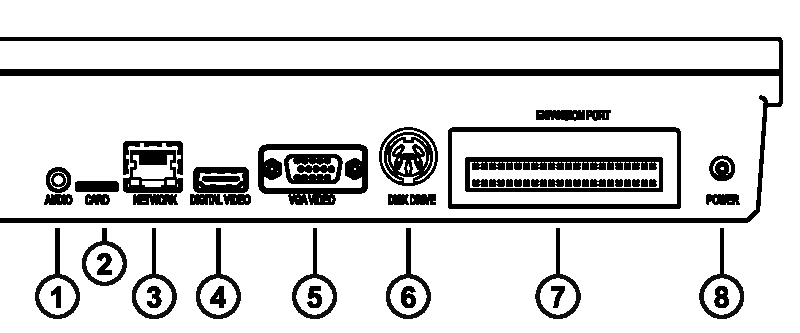
\includegraphics[width=\linewidth]{images/illustrations/mega65-rear.pdf}
\begin{center}
\setlength{\def\arraystretch{1.5}\tabcolsep}{6pt}
\begin{longtable}{ c | l}
	1	& 	3.5 mm-audiojack \\	2	& 	Externe microSD-kaartsleuf\\	3	& 	Netwerk-LAN-poort \\	4	& 	Digitale video-aansluiting (inclusief geluid) \\	5	& 	VGA-videoaansluiting \\	6	& 	Seriële IEC-bus-aansluiting voor schijfstations en printers \\	7	& 	Cartridge-uitbreidingspoort \\	8	& 	Voedingsaansluiting \\
\end{longtable}
\end{center}

\vspace{-1cm}

\section{Aansluitingen aan de zijkant}

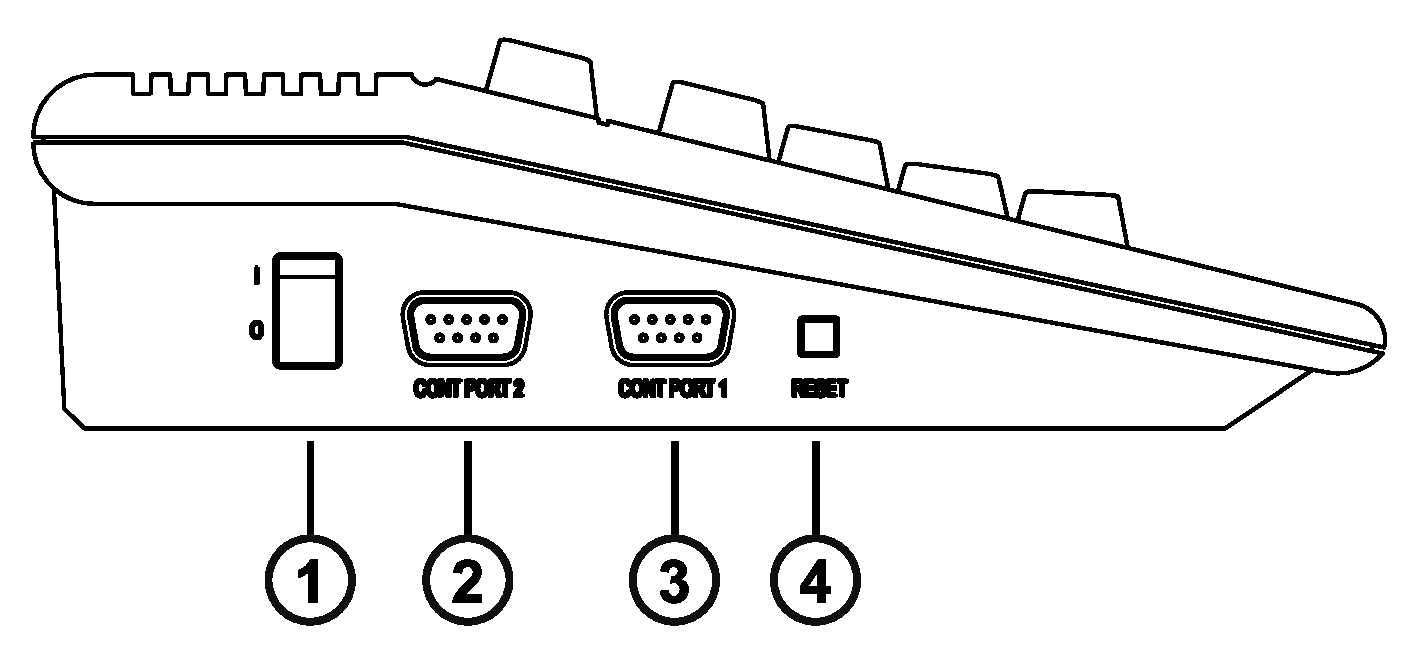
\includegraphics[width=\linewidth]{images/illustrations/mega65-side.pdf}

\begin{center}
\setlength{\def\arraystretch{1.5}\tabcolsep}{6pt}
\begin{longtable}{ c | l}
	1	& 	Aan/uit-schakelaar \\	2	& 	Controllerpoort 2 \\	3	& 	Controllerpoort 1 \\	4	& 	Resetknop \\
\end{longtable}
\end{center}

Op controllerpoorten 1 en 2 kunt u diverse randapparatuur aansluiten, zoals joysticks, peddels of muizen.

\newpage

\section{Beeldscherm en randapparatuur}

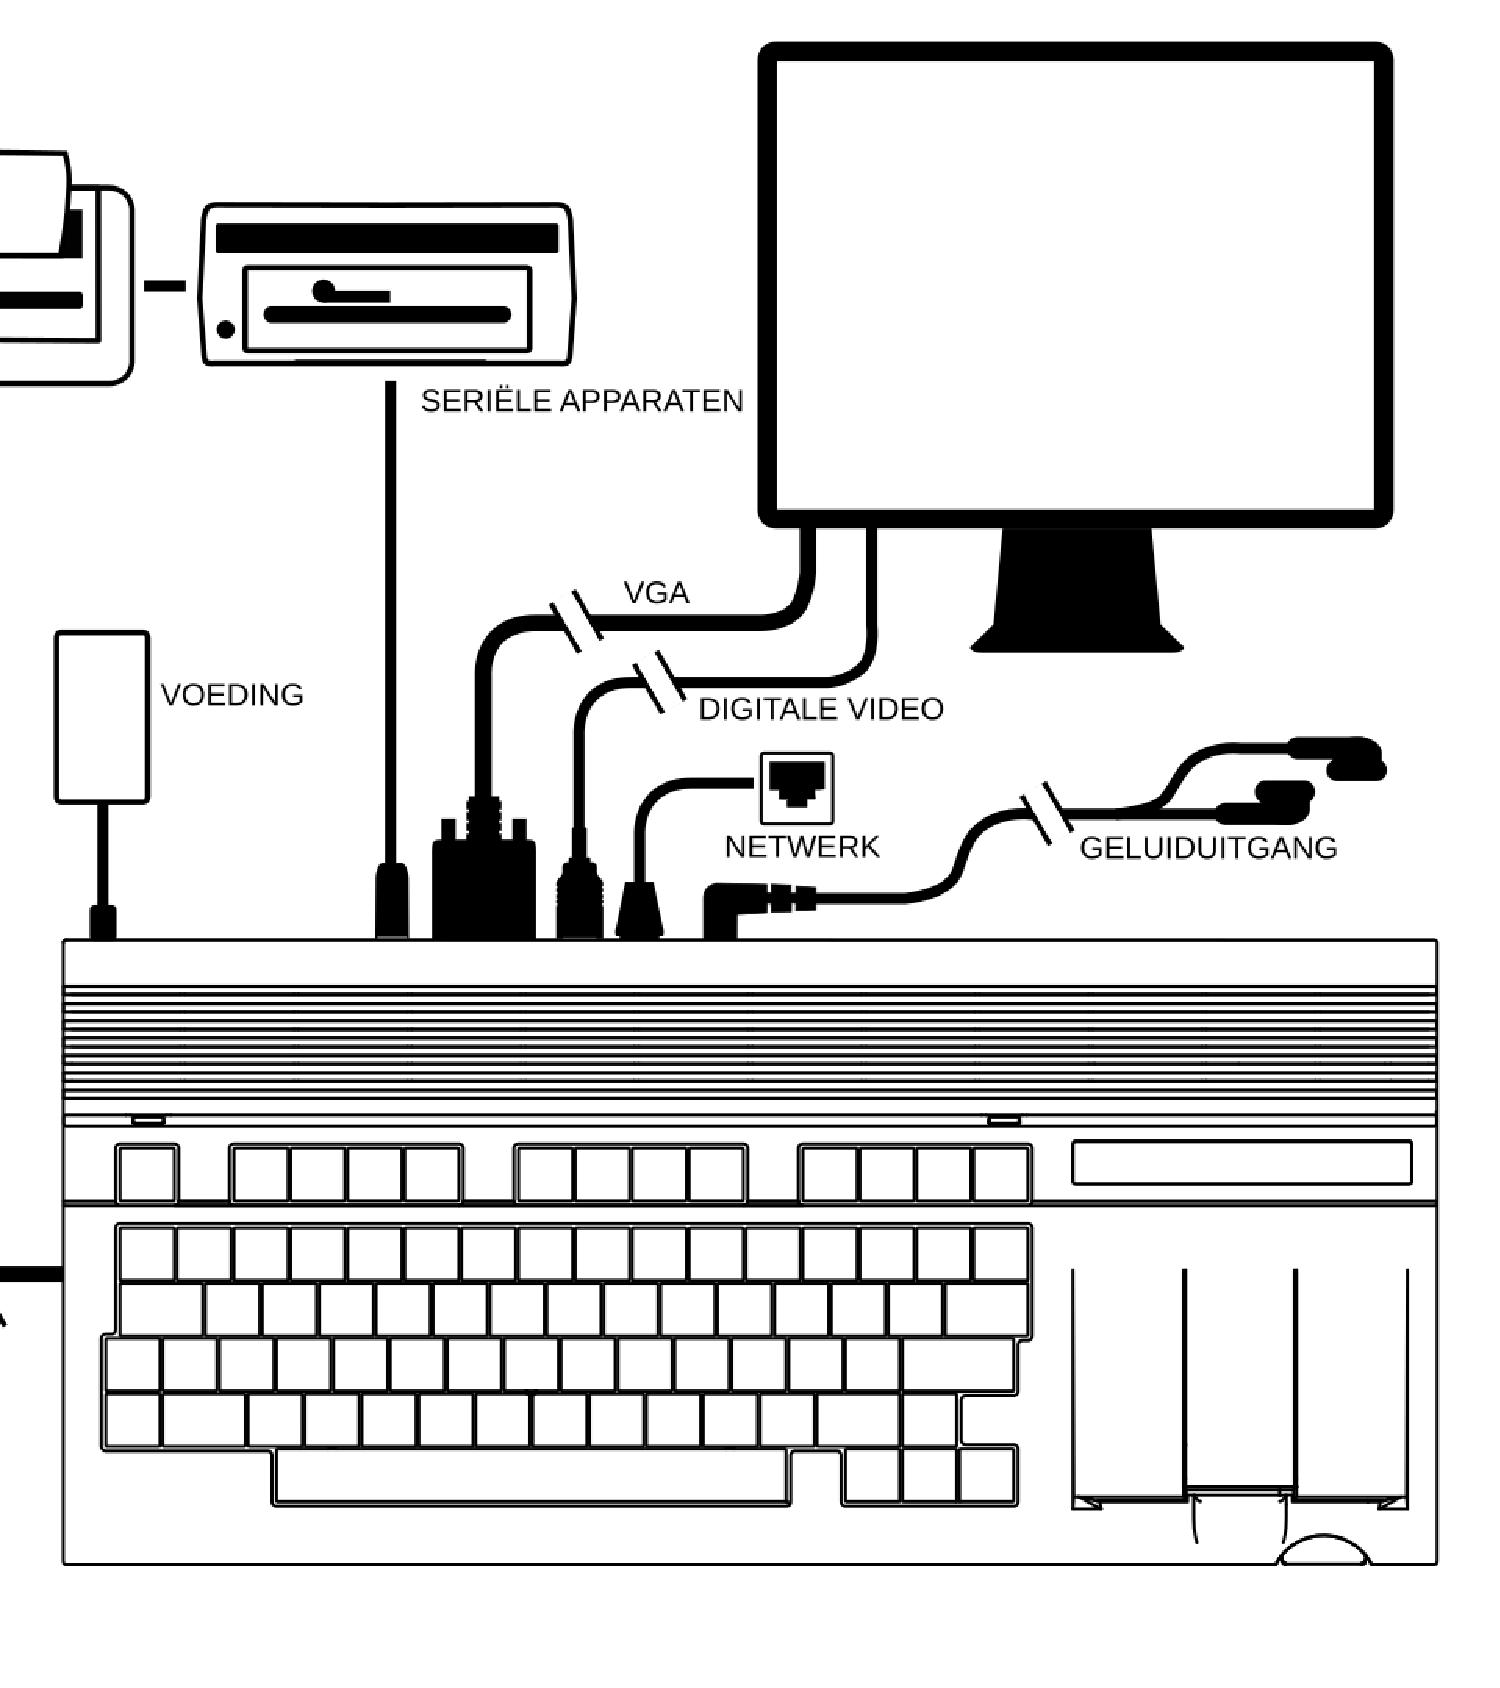
\includegraphics[width=\linewidth]{dutch/images/illustrations/mega65-top.pdf}

U sluit uw MEGA65 als volgt op een beeldscherm aan:
\index{Scherm!Aansluiten}

\begin{enumerate}
	\item Sluit de voeding aan op de voedingsaansluiting van de MEGA65.	\item Als u een VGA-monitor en een VGA-kabel hebt, sluit u het ene uiteinde aan op de VGA-poort van de MEGA65 en het andere uiteinde op uw VGA-monitor.	\item Als u een tv of monitor met een compatibele Digital Video-aansluiting hebt,\footnote{Het type Digital Video-aansluiting heeft een herkenbare commerciële naam van vier letters, doch het MEGA65-project heeft geen licentiekosten betaald om naar dit type met deze naam te verwijzen. Deze {\em Gebruikershandleiding} verwijst hiernaar als de ``Digital Video''-aansluiting.}\index{Digitale video} sluit u het ene uiteinde van uw kabel aan op de Digital Video-poort van de MEGA65 en het andere uiteinde op de Digital Video-poort van uw monitor. Als u een monitor met een DVI-aansluiting hebt, kunt u een Digital Video-naar-DVI-adapter gebruiken.
\end{enumerate}

\newpage
\section{Optionele aansluitingen}
\index{Schijfstations!Aansluiten}
\index{Aansluitingen!IEC}
\index{SD-kaarten!Locaties}
\begin{enumerate}
	\item De MEGA65 bevat een ingebouwd 3.5 inch-diskettestation. U kunt ook oudere Commodore{\textregistered}-diskettestations via de seriële IEC-bus aansluiten, zoals de Commodore 1541, 1571 of 1581. Sluit om deze stations te gebruiken het ene uiteinde van een IEC-kabel aan op het Commodore-diskettestation en het andere uiteinde op de schijfstationsaansluiting van de MEGA65. U kunt ook een SD2IEC-apparaat\index{SD2IEC-apparaat} of een Pi1541-apparaat aansluiten.\index{Pi1541-apparaat} Bij de meeste apparaten kunt u extra diskettestations of met Commodore compatibele printers aan elkaar koppelen.	\item U kunt uw MEGA65 met een standaard ethernetkabel aansluiten op een ethernetnetwerk.	\item Om naar audio van uw MEGA65 te luisteren, kunt u een 3.5 mm-audiojackkabel aansluiten op een audioversterker of een luidsprekersysteem. Als uw systeem over RCA-aansluitingen beschikt, hebt u een 3.5 mm-audiojack-naar-twin-RCA-adapterkabel nodig. De MEGA65 heeft tevens een ingebouwde versterker, zodat u een hoofdtelefoon kunt gebruiken.	\item U kunt een microSD-kaart, type SDHC tussen 4GB en 32GB, in de externe microSD-kaartsleuf aan de achterzijde van de MEGA65 steken. Zie voor meer informatie over het gebruik van de microSD-kaartsleuf ``Kennismaken met SD-kaarten'' op bladzijde \pageref{sec:introducing-sd-cards}.	\item Aan de onderzijde van de MEGA65 geeft een klein klepje toegang tot de interne SD-kaart en twee aansluitingen voor toekomstige hardware-uitbreidingen.
\end{enumerate}

\index{Real-time klok!Batterij plaatsen}
\subsection{De batterij van de real-time klok installeren}

De MEGA65 bevat een real-time klok, welke wordt gebruikt om de tijd en datum op het opstartscherm weer te geven, om tijdstempels toe te voegen aan bestanden die de MEGA65 op uw SD-kaarten schrijft en om de {\bf DT\$}\index{BASIC 65-variabelen!DT} en {\bf TI\$}\index{BASIC 65-variabelen!TI\$}-BASIC-variabelen voor gebruik in programma's te verschaffen. Deze klok gebruikt een CR2032-knoopcelbatterij om de tijd bij te houden wanneer de MEGA65 gedurende langere perioden van de voeding is losgekoppeld. De MEGA65 wordt niet met een batterij geleverd, om problemen met het internationaal verzenden van batterijen te vermijden.\footnote{Vroege modellen van de MEGA65 met de ``R3A''-printplaatrevisie (gemaakt in het jaar 2022) gebruiken een batterij van het type CR1220 voor de real-time klok en de batterij is vereist om de RTC te laten functioneren. Revisie ``R6'' (gemaakt in 2024) gebruikt een batterij van het type CR2032 en de batterij is optioneel voor normaal gebruik.}

{\bf De RTC-batterij is optioneel.} De MEGA65 kan de RTC zonder batterij draaiende houden, zelfs wanneer de computer gedurende meerdere dagen achter elkaar van de voeding is losgekoppeld. Met een batterij kan de computer de tijd gedurende veel langere perioden onthouden. U kunt de klok later altijd opnieuw instellen.

Schakel de computer uit om de batterij te installeren. Gebruik een kruiskopschroevendraaier om de behuizing te openen, waardoor het moederbord zichtbaar wordt.\index{Behuizing!Opening} De behuizing wordt bijeengehouden door drie schroeven, allemaal langs de onderkant van de voorzijde van de behuizing. Til, nadat de schroeven zijn verwijderd, voorzichtig de bovenste helft van de behuizing op. Let op de oriëntatie van de toetsenbordaansluiting en koppel deze vervolgens los.

De batterij bevindt zich tussen de controllerpoorten en de toetsenbordaansluiting.

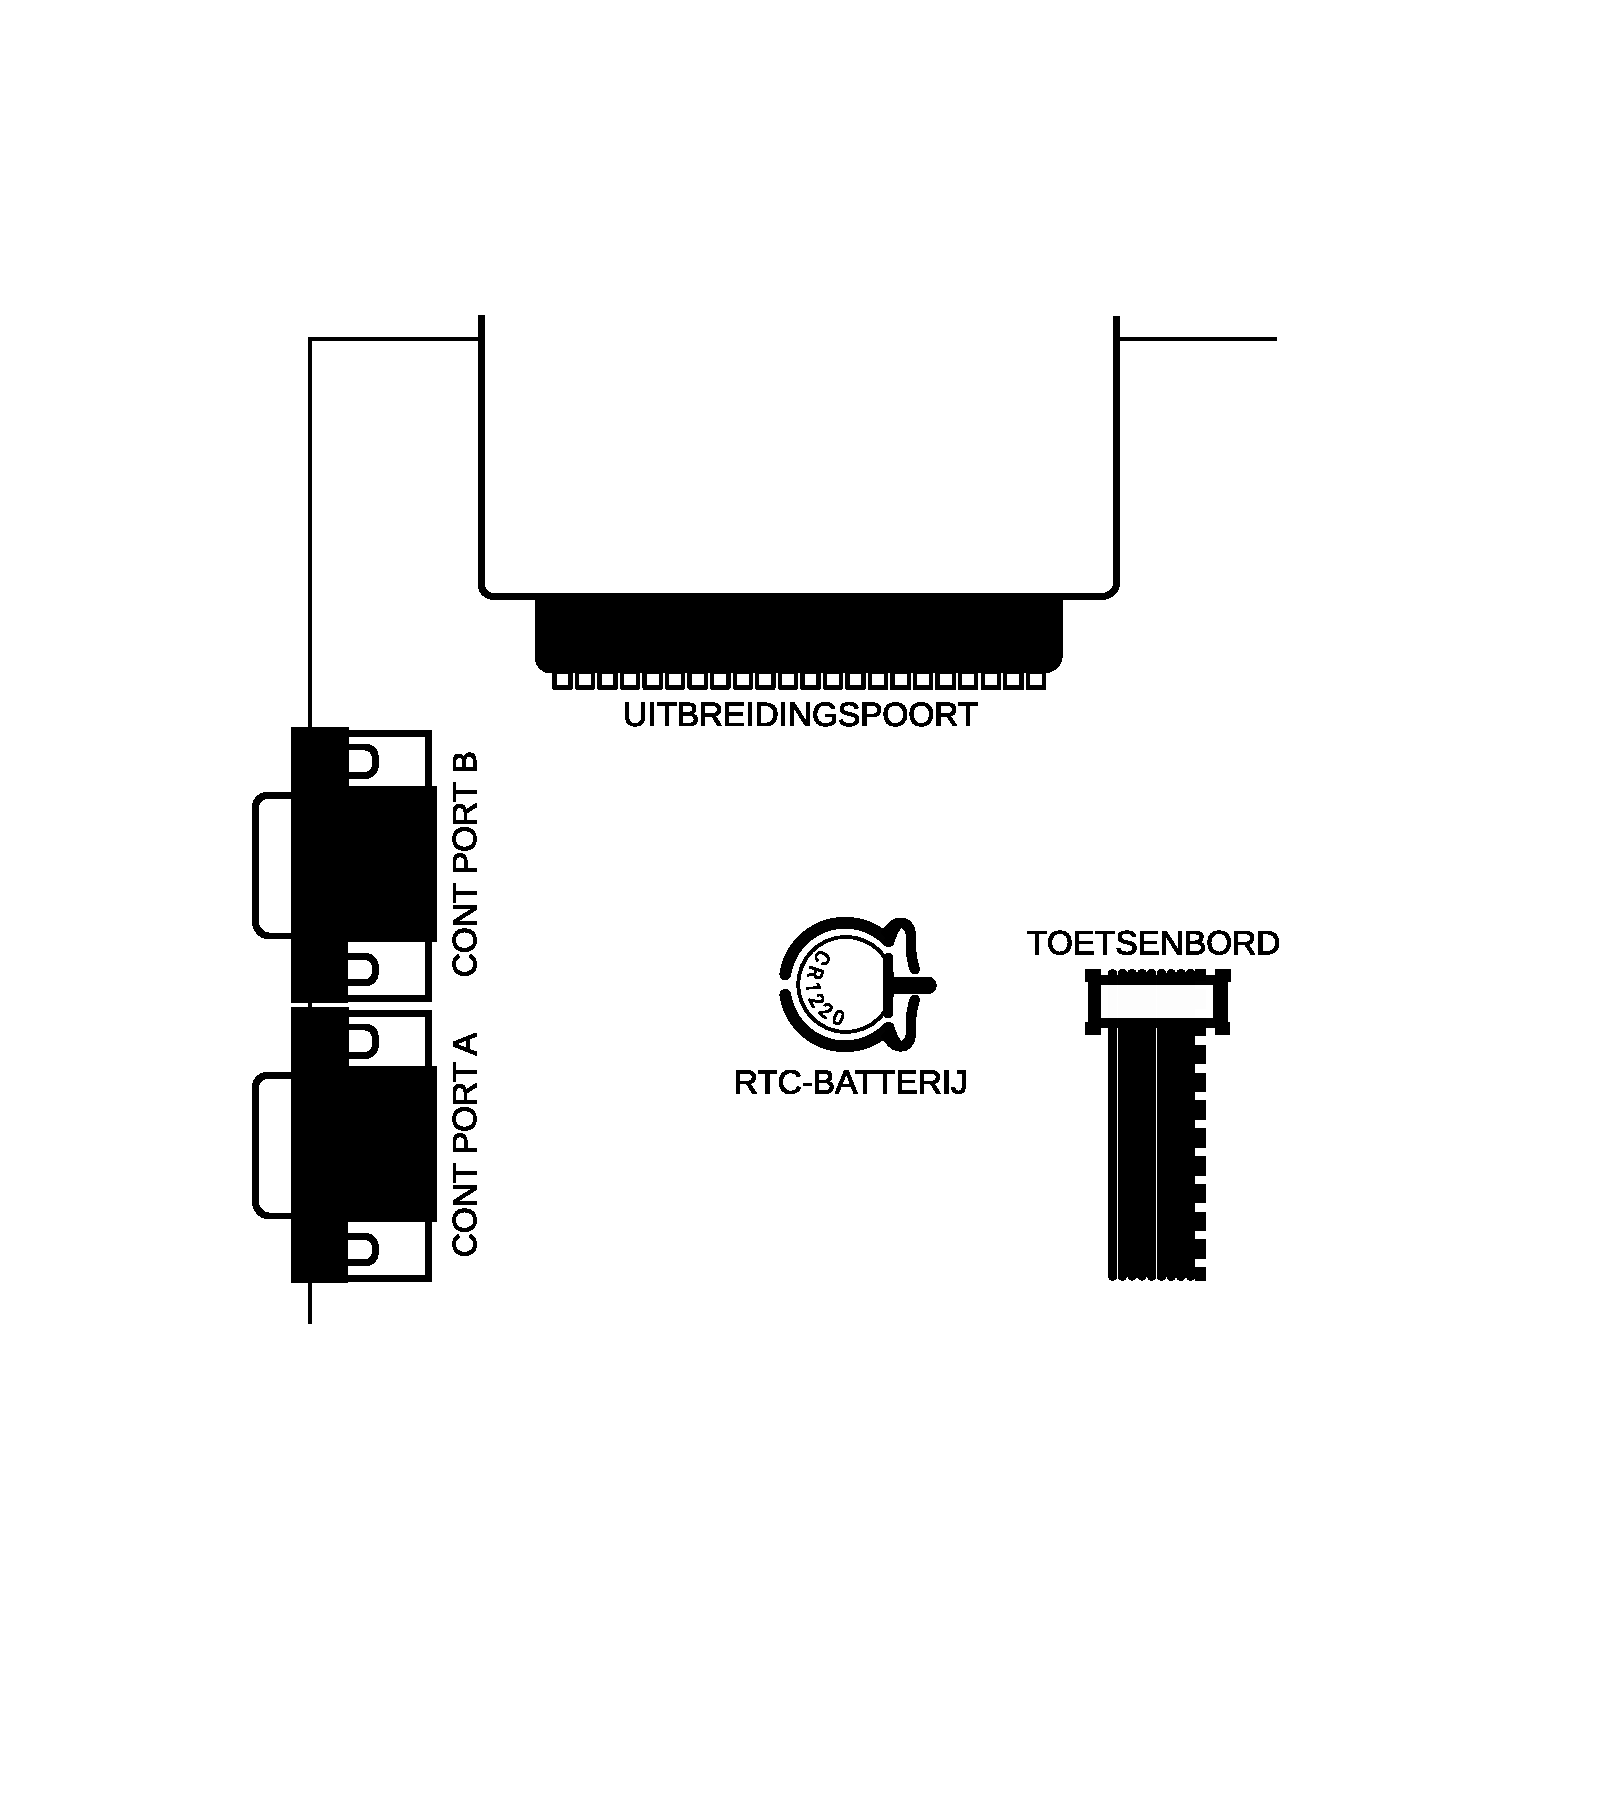
\includegraphics[width=\linewidth]{dutch/images/illustrations/rtc-battery-location.pdf}

Indien u een bestaande batterij verwijdert, duwt u de ontgrendelingshendel van de batterij aan de onderkant (de platte zijde) van de batterijhouder weg van de batterij om deze te verwijderen. Plaats de nieuwe batterij met de positieve zijde (gemarkeerd met {\bf +}) naar boven gericht en druk hem op zijn plaats.

Zodra u uw MEGA65 weer in elkaar hebt gezet, kunt u in het configuratiehulpprogramma de tijd instellen. Zie voor meer informatie over het instellen van de real-time klok het onderdeel over het configuratiehulpprogramma op bladzijde \pageref{sec:configuration-utility}.


\newpage

\section{De MEGA65 inschakelen}
\label{onboarding}

Schakel de MEGA65 in met de aan/uit-schakelaar aan de linkerkant van de computer.

Wanneer u uw MEGA65 voor het eerst inschakelt, toont de computer het scherm voor de initiële configuratie (``on-boarding'').\index{Configuratie!Introductie} Op dit scherm kunt u de tijd en de datum op de real-time klok instellen, de videomodus wijzigen en het geluid testen. Al deze instellingen kunt u later nog wijzigen.

\begin{center}
  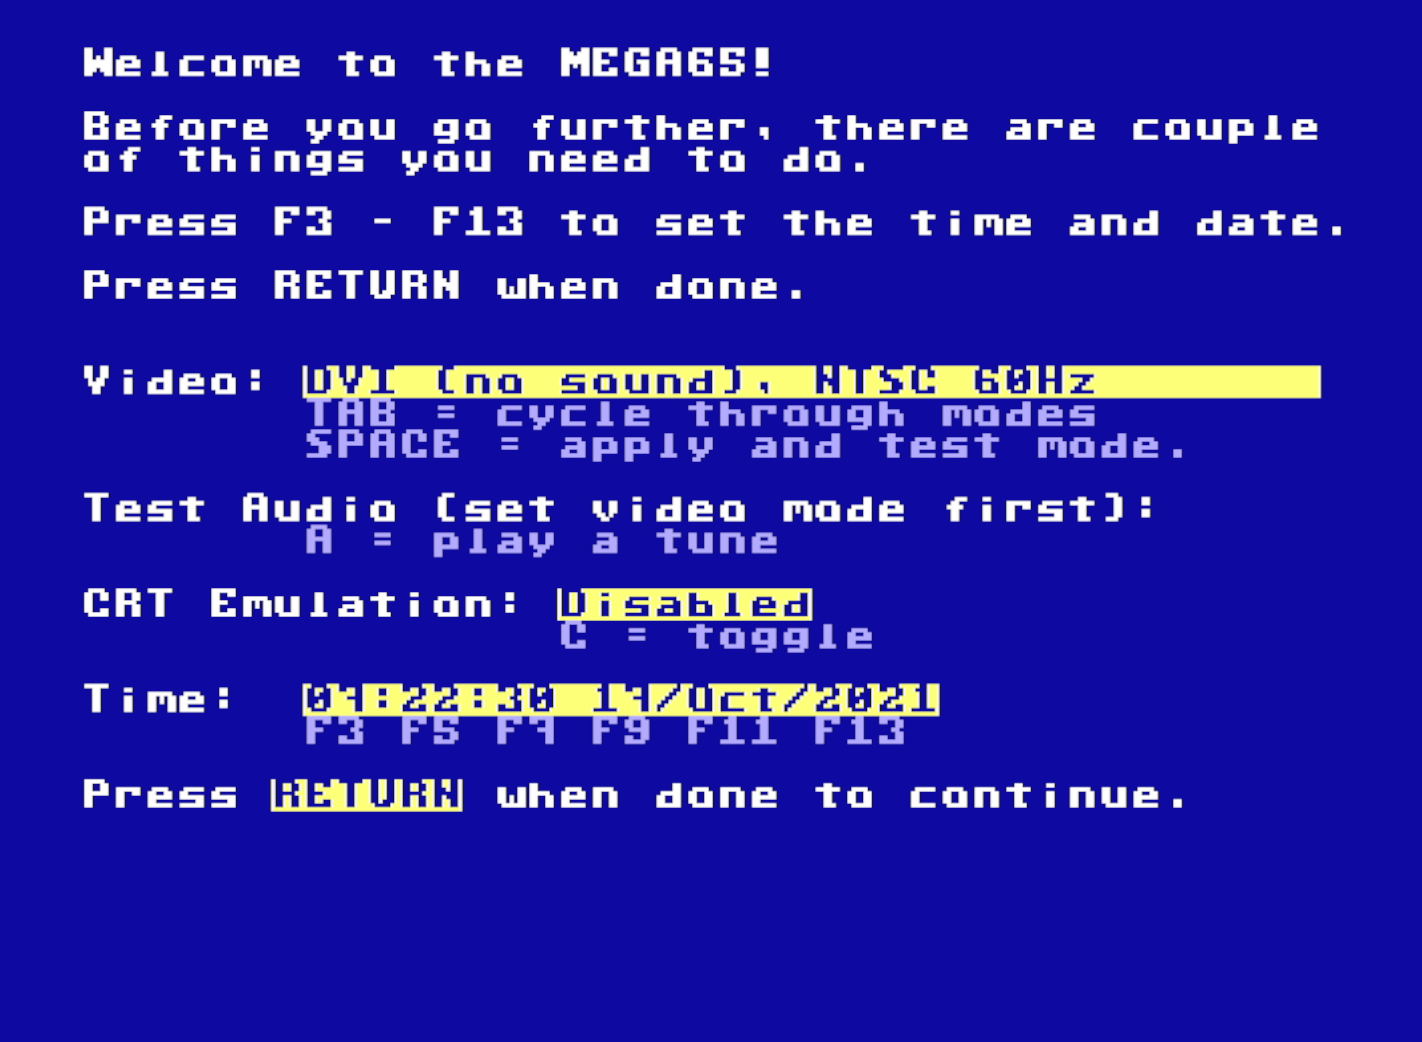
\includegraphics[width=0.7\linewidth]{images/img011_final_boot_01.png}
\end{center}

Voor videomodi kunt u kiezen tussen PAL-emulatie\index{PAL-schermmodus} en NTSC-emulatie\index{NTSC-schermmodus}. Daarnaast kunt u aangeven of uw Digital Video-beeldscherm geluid ondersteunt. Indien u de VGA-videouitgang gebruikt, heeft de Digital Video-geluidsmodus geen effect.

\underline{OPMERKING}: Een DVI-beeldscherm dat geen geluid ondersteunt, werkt niet met de ``enhanced''-geluidsmodus. Bij een dergelijk beeldscherm moet u een videomodus met ``no sound'' selecteren en een luidspreker op de 3.5 mm-audioaansluiting aansluiten.

PAL en NTSC zijn analoge videosignaalformaten die de resolutie en de verticale synchronisatiesnelheid van de videouitgang beïnvloeden, ook wanneer u een modern digitaal beeldscherm gebruikt. Uw beeldscherm ondersteunt mogelijk beide modi of slechts één van beide. U kunt dit scherm gebruiken om de modi met uw beeldscherm te testen.

Selecteer en test uw videoconfiguratie. Druk bijvoorbeeld op \specialkey{TAB} om naar de modus {\bf PAL 50Hz} over te schakelen.
\index{Scherm!PAL/NTSC instellen}
\begin{center}
  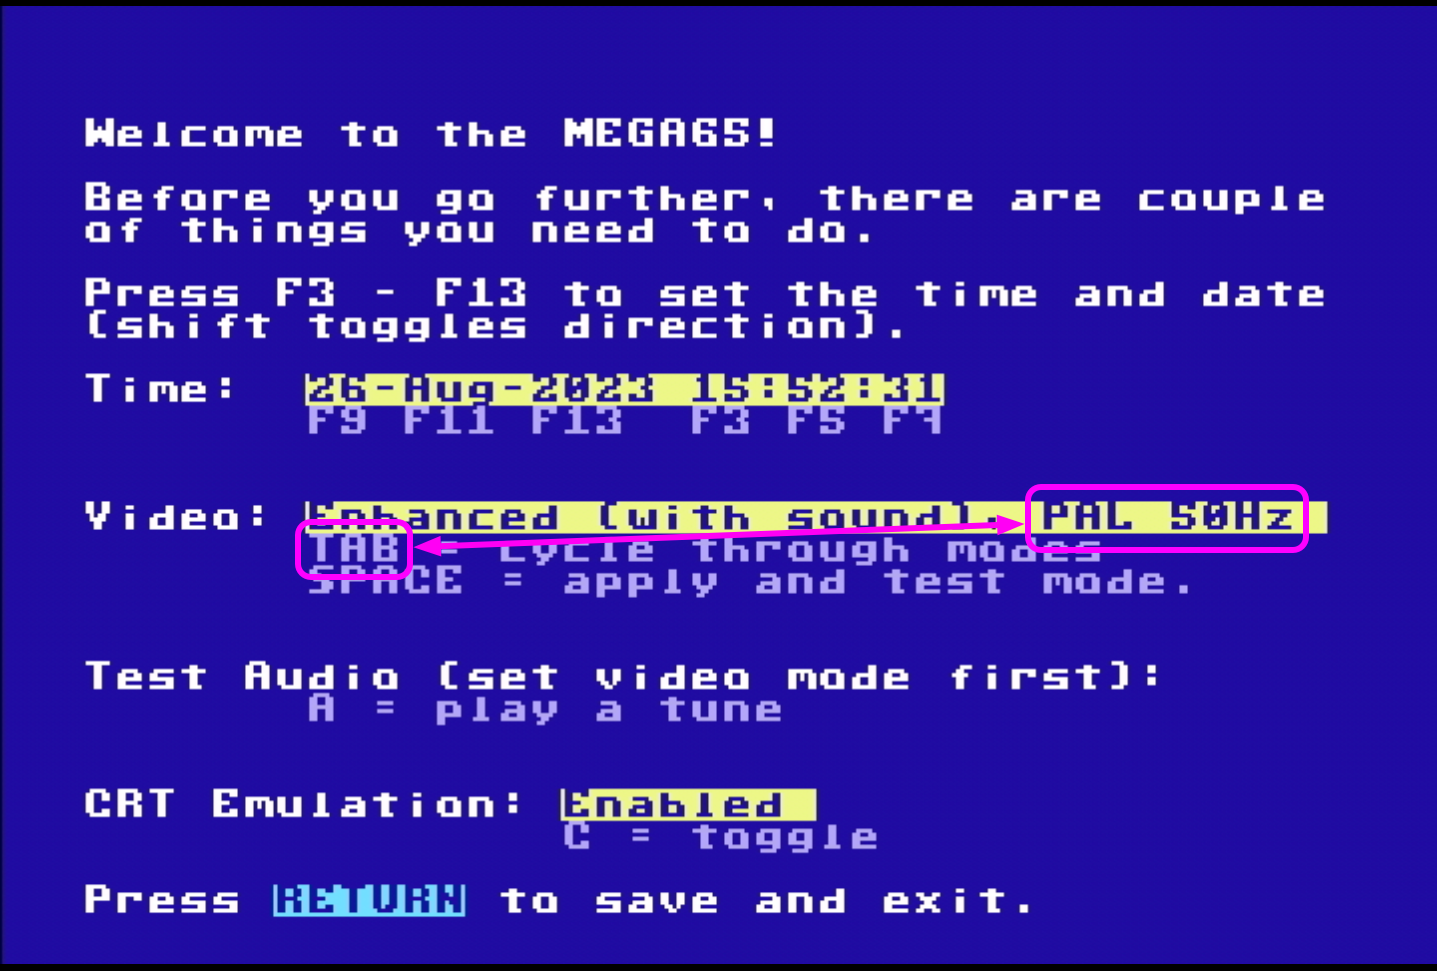
\includegraphics[width=0.7\linewidth]{images/img011_final_boot_02.png}
\end{center}

Druk op \megakey{SPACE} en vervolgens op \megakey{Y} om de nieuwe videomodus te testen.

\begin{center}
  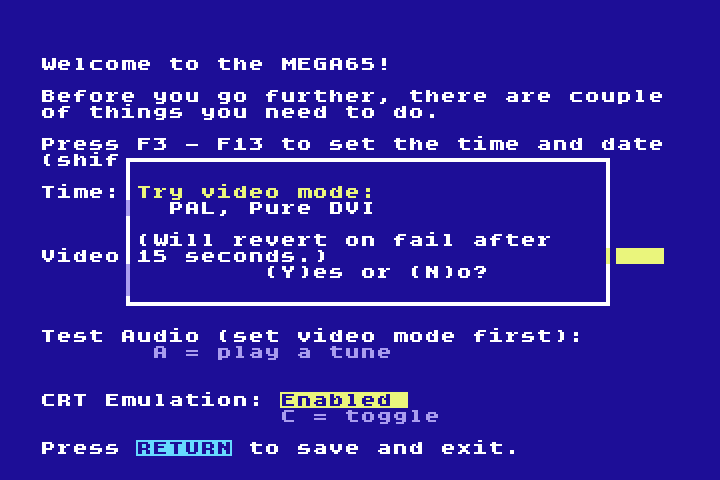
\includegraphics[width=0.7\linewidth]{images/img011_final_boot_03.png}
\end{center}

Druk op \megakey{K} om de nieuwe videomodus te behouden.

\begin{center}
  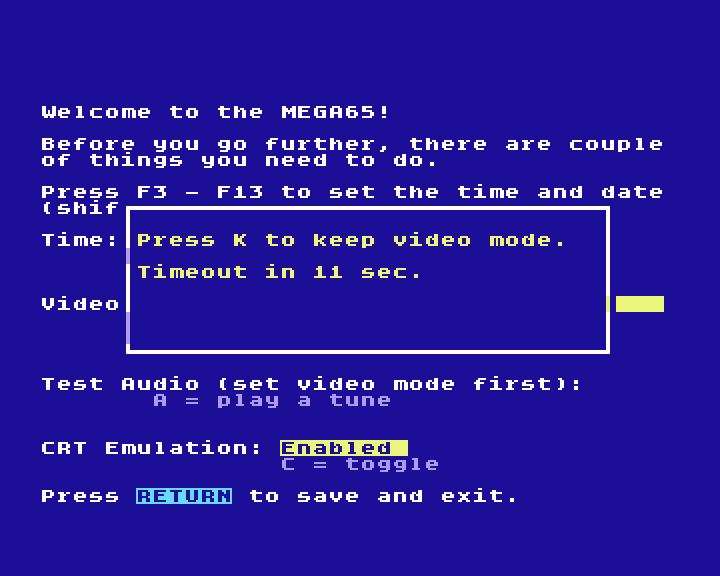
\includegraphics[width=0.7\linewidth]{images/img011_final_boot_04.png}
\end{center}

Maak van deze gelegenheid gebruik om uw geluidsopstelling te testen. Druk op \megakey{A} om een geluid af te spelen.

De optie ``CRT Emulation'' is een leuke keuze bij gebruik van een modern plat scherm. Deze optie voegt verticale tussenruimten toe tussen de pixels om de rasterlijnen van een beeldbuis na te bootsen. Probeer het om te zien of het u bevalt: druk op de toets \megakey{C} om de optie in en uit te schakelen.

Druk ten slotte op \specialkey{RETURN} om de configuratie af te ronden.

Zie voor meer informatie over het configureren van uw MEGA65 hoofdstuk \vref{cha:configuringyourmega}.

\section{De Intro Disk}
\index{Intro Disk}

Nadat u de initiële configuratie hebt afgerond, start uw MEGA65 het Intro Disk-menu. De Intro Disk is een verzameling software van de MEGA65-gemeenschap die enkele van de mogelijkheden van de computer demonstreert. Neem de tijd om door de menu's te bladeren en een aantal demo's uit te proberen. Druk na elke demo op de resetknop aan de linkerkant van de computer om terug te keren naar het Intro Disk-menu.

\begin{center}
  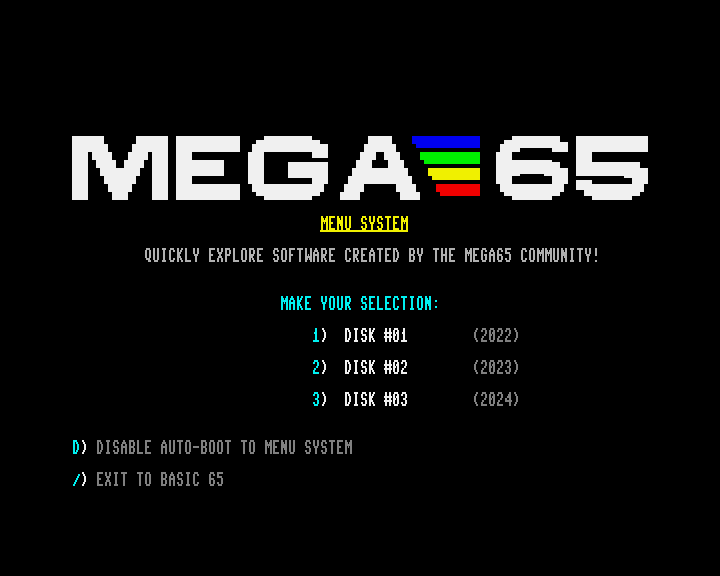
\includegraphics[width=0.7\linewidth]{images/demo_title.png}
\end{center}

Standaard opent het Intro Disk-menu telkens wanneer u de computer inschakelt. Zodra u meer vertrouwd bent met de MEGA65, wilt u dit wellicht uitschakelen. Druk bij het Intro Disk-menu op \megakey{D} om de automatische opstartfunctie van de Intro Disk uit te schakelen.\index{Intro Disk!Uitschakelen}

Druk op \megakey{/} (de schuine streep) om het Intro Disk-menu te verlaten en toegang te krijgen tot BASIC 65. Indien de automatische opstartfunctie van de Intro Disk is uitgeschakeld, gaat de MEGA65 bij het inschakelen rechtstreeks naar BASIC 65.

\begin{center}
  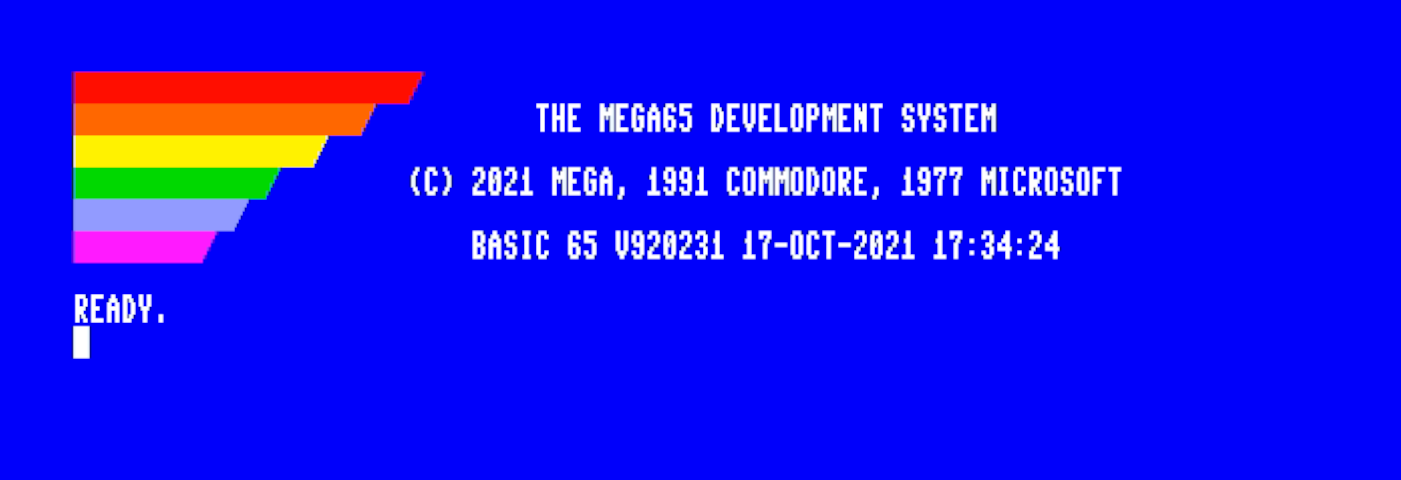
\includegraphics[width=0.7\linewidth]{images/img011_final_boot_06.png}
\end{center}

\section{De cursor}

Het knipperende blokje onder de \screentext{READY}-prompt\index{READY-prompt} wordt de \emph{cursor} genoemd. De cursor geeft aan dat de computer klaar is om invoer te ontvangen. Wanneer u toetsen op het toetsenbord indrukt, verschijnen de bijbehorende tekens op het scherm. De tekens verschijnen op de huidige cursorpositie en de cursor schuift na elke toetsaanslag een positie op.

Hier kunt u commando's typen waarmee u bijvoorbeeld een programma kunt laden. U kunt ook beginnen met het intypen van programmacode!

\chapter{Aan de slag}\addtocontents{toc}{\protect\setcounter{tocdepth}{2}}
\hypersetup{bookmarksdepth=5}

\section{Toetsenbord}
\label{cha:getting-started}
\index{Toetsenbord}

Nu alles is aangesloten, is het tijd om vertrouwd te raken met het toetsenbord van de MEGA65.

Wellicht valt u op dat het toetsenbord enigszins afwijkt van de toetsenborden van andere hedendaagse computers. De meeste toetsen staan op vertrouwde posities, maar er zijn enkele gespecialiseerde toetsen en sommige toetsen hebben speciale grafische symbolen op de voorkant.

In sommige beeldschermmodi zijn de grafische symbolen te typen, net als letters, cijfers en leestekens. De volledige verzameling tekens staat bekend als de {\em PETSCII-tekenset}.\index{PETSCII}

\subsection{Speciale toetsen}

\subsubsection{RETURN}
\index{Toetsenbord!RETURN}
Wanneer u op \specialkey{RETURN} drukt, slaat de computer de informatie die u hebt getypt op in het geheugen. De computer voert vervolgens een opdracht uit, bewaart enkele gegevens of toont een foutmelding indien u een vergissing hebt gemaakt.

\subsubsection{SHIFT}
\index{Toetsenbord!Shifttoetsen}
De twee \specialkey{SHIFT}-toetsen bevinden zich links en rechts. Zij werken vrijwel hetzelfde als de Shift-toets van een gewoon toetsenbord en vervullen daarnaast nog enkele speciale functies.

In de modus met hoofdletters levert het ingedrukt houden van \specialkey{SHIFT} en het indrukken van een toets met twee grafische symbolen op de voorkant het rechter symbool van die toets op. Zo toont \specialkey{SHIFT} samen met \megakey{J} het teken \graphicsymbol{J}.

In de modus met kleine letters geeft het indrukken van \specialkey{SHIFT} en een lettertoets de hoofdletter van die toets weer.

Om de Griekse letter $\pi$ (pi) te typen, houdt u \specialkey{SHIFT} ingedrukt en drukt u op \megakeywhite{$\uparrow$}.

Het ingedrukt houden van \specialkey{SHIFT} en het indrukken van een functietoets roept de functie op die op de voorkant van die toets staat vermeld. Zo activeert \specialkey{SHIFT} samen met \megakey{F1} de functie \megakey{F2}.


\subsubsection{SHIFT LOCK}
\index{Toetsenbord!SHIFT LOCK}
Naast \specialkey{SHIFT} is er de \specialkey{SHIFT\\LOCK}-toets. Druk op deze toets om de Shift-functie vast te zetten. Wanneer \specialkey{SHIFT\\LOCK} verlicht is, toont elke toets die u indrukt het bijbehorende teken op het scherm, alsof u \specialkey{SHIFT} ingedrukt houdt. Dit geldt ook voor speciale grafische tekens.

\subsubsection{CTRL}
\index{Toetsenbord!CTRL}
\specialkey{CTRL} is de Control-toets. Door \specialkey{CTRL} ingedrukt te houden en een andere toets in te drukken, kunt u Controlcodes uitvoeren. Zo kunt u met \specialkey{CTRL} ingedrukt en één van de cijfertoetsen (van \megakey{1} tot \megakey{8}) de tekstkleur wijzigen. De kleur die op de bovenste rij van de voorkant van de cijfertoets is afgedrukt, wordt gebruikt. Het ingedrukt houden van \specialkey{CTRL} en het indrukken van \megakey{9} of \megakey{0} schakelt de modus voor omgekeerde tekst in en uit.

Enkele voorbeelden hiervan vindt u op bladzijde \pageref{sec:screen-editor} en alle Controlcodes staan vermeld op bladzijde \pageref{appendix:controlcodes}.

Wanneer een programma met {\bf LIST} op het scherm wordt weergegeven, vertraagt het ingedrukt houden van \specialkey{CTRL} de weergave van elke regel. Meer over het commando {\bf LIST} leest u op bladzijde \pageref{BASIC 65 Commands!LIST}.\index{BASIC 65-commando's!LIST}

Het ingedrukt houden van \specialkey{CTRL} en het indrukken van \megakey{*} opent de Matrix Mode Debugger (raadpleeg {\bf Het grote Mega65-boek} voor meer details).

\subsubsection{RUN/STOP}
\index{Toetsenbord!RUN STOP}
Normaal gesproken stopt het indrukken van \specialkey{RUN\\STOP} de uitvoering van een programma. Wanneer u \specialkey{SHIFT} ingedrukt houdt en op \specialkey{RUN\\STOP} drukt, voert u met {\bf RUN} het eerste programma van de schijf uit.\index{BASIC 65-commando's!RUN}

Sommige programma's onderscheppen de \specialkey{RUN\\STOP}-toets en kunnen op deze wijze niet worden gestopt.

U kunt uw MEGA65 naar de {\bf Machinetaalmonitor}\index{Machinetaalmonitor} opstarten door \specialkey{RUN\\STOP} ingedrukt te houden en de resetknop aan de linkerkant van de computer in te drukken (of door de toets ingedrukt te houden terwijl u de computer inschakelt).

\subsubsection{RESTORE}
\index{Toetsenbord!RESTORE}
Het computerscherm kan naar een schone toestand worden teruggebracht zonder het geheugen te wissen door \specialkey{RUN\\STOP} ingedrukt te houden en \widekey{RESTORE} in te drukken. Deze combinatie herstelt tevens de vectoren van het besturingssysteem en initialiseert de schermeditor opnieuw, hetgeen dit tot een handige combinatie maakt indien de computer een beetje in de war is geraakt.

Sommige programma's onderscheppen de toetsencombinatie \specialkey{RUN\\STOP} + \widekey{RESTORE} en kunnen op deze wijze niet worden gereset.

U kunt de {\bf Freezer} ook oproepen door \widekey{RESTORE} één seconde ingedrukt te houden en de toets vervolgens los te laten. U kunt meer over de Freezer lezen op bladzijde \pageref{sec:freezer}.\index{Freezer-menu}

\subsubsection{De cursor-toetsen}
\index{Toetsenbord!Cursortoetsen}
\nopagebreak
De cursor-toetsen staan rechtsonder op het toetsenbord. Met deze vier richtingtoetsen kunt u de cursor naar elke gewenste positie verplaatsen voor het bewerken van tekst op het scherm.

De cursor beweegt in de richting die op de toetsen is aangegeven: \megakey{$\leftarrow$} \megakey{$\uparrow$} \megakey{$\rightarrow$} \megakey{$\downarrow$}.

U hoeft een cursor-toets niet telkens opnieuw in te drukken. Indien u de cursor over een grote afstand moet verplaatsen, kunt u de toets ingedrukt houden. Wanneer u klaar bent, laat u de toets gewoon los.

\subsubsection{De pijltjestoetsen}
\index{Toetsenbord!Pijltjestoetsen}
Deze toetsen verschillen van de cursor-toetsen. Het zijn \megakeywhite{$\leftarrow$} (naast \megakey{1}) en \megakeywhite{$\uparrow$} (naast \widekey{RESTORE}). Beide pijltjestoetsen worden gebruikt in diverse BASIC-functies en escape-sequenties.

Zo kan \megakeywhite{$\leftarrow$} als snelkoppeling voor {\bf SAVE}\index{BASIC 65-commando's!SAVE} dienen en wordt \megakeywhite{$\uparrow$} gebruikt om een getal tot een macht te verheffen (hetgeen gelijkstaat aan het getal een opgegeven aantal malen met zichzelf te vermenigvuldigen).

U kunt meer lezen over de beschikbare escape-sequenties op bladzijde \pageref{escape-sequences}.

Deze twee PETSCII-specifieke toetsen worden in de MEGA65-literatuur altijd met een witte achtergrond weergegeven.

Het is ook mogelijk de cursor met \specialkey{SHIFT} en \megakey{$\downarrow$} omhoog en met \specialkey{SHIFT} en \megakey{$\rightarrow$} naar links te verplaatsen. Dit is een erfenis van de Commodore 64, welke slechts twee cursor-toetsen had.

\subsubsection{INSerT/DELete}
\index{Toetsenbord!INST DEL}
De toets \specialkey{INST\\DEL}, de meest rechtse toets van de bovenste rij, is de INSERT/DELETE-toets. Wanneer u \specialkey{INST\\DEL} indrukt, wordt het teken links daarvan verwijderd en worden alle tekens rechts daarvan één positie naar links verschoven.

Om een teken in te voegen, houdt u \specialkey{SHIFT} ingedrukt en drukt u op \specialkey{INST\\DEL}. Het teken onder de cursor en de tekens rechts van de cursor worden naar rechts verschoven. Op de nieuw vrijgekomen plaats kunt u vervolgens een letter, een cijfer of elk ander teken typen.


\subsubsection{CLeaR/HOME}
\index{Toetsenbord!CLR HOME}
De toets \specialkey{CLR\\HOME} is de CLEAR/HOME-toets. Het indrukken van \specialkey{CLR\\HOME} verplaatst de cursor naar de linkerbovenhoek van het scherm.

Door \specialkey{SHIFT} ingedrukt te houden en op \specialkey{CLR\\HOME} te drukken, wist u het volledige scherm {\it en} plaatst u de cursor in de linkerbovenhoek van het scherm.

Indien u per ongeluk \specialkey{CLR\\HOME} indrukt, kunt u de cursor naar zijn vorige positie terugbrengen door \specialkey{ESC} en vervolgens \specialkey{CLR\\HOME} in te drukken.

\subsubsection{De MEGA-toets}
\index{Toetsenbord!MEGA-toets}
De \megasymbolkey of de MEGA-toets biedt een aantal verschillende functies en kan worden gebruikt om speciale hulpprogramma's op te starten.

Door \specialkey{SHIFT} ingedrukt te houden en \megasymbolkey in te drukken, schakelt u tussen de kleine- en de hoofdlettermodus.

Door \megasymbolkey ingedrukt te houden en een willekeurige toets met twee grafische symbolen op de voorkant in te drukken, geeft de computer het meest linkse grafische symbool op het scherm weer. Zo geven \megasymbolkey en \megakey{D} het symbool \graphicsymbol{d} weer.

Door \megasymbolkey ingedrukt te houden en een cijfertoets in te drukken, schakelt u over naar een secundaire kleur, d.w.z. de kleur die op de onderste rij aan de voorkant van de cijfertoets is afgedrukt.

Door \megasymbolkey ingedrukt te houden en \specialkey{TAB} in te drukken, opent u de Matrix Mode Debugger (zie voor meer details {\bf Het grote Mega65-boek}).

Indien u de MEGA65 inschakelt, of de resetknop aan de linkerkant indrukt terwijl u \megasymbolkey ingedrukt houdt, schakelt de MEGA65 over naar de GO64-modus.\index{Commodore 64!GO64-modus}

\subsubsection{NO SCROLL}
\index{Toetsenbord!NO SCROLL}
Indien een programma met {\bf LIST} naar het scherm wordt afgedrukt, onderbreekt u de schermuitvoer door \specialkey{NO\\SCROLL} in te drukken. Druk een willekeurige toets in om de pauze op te heffen.

Deze functie is niet beschikbaar in de GO64-modus.\index{Commodore 64!GO64-modus}

\subsubsection{De functietoetsen}
\index{Toetsenbord!Functietoetsen}
Er zijn zeven functietoetsen beschikbaar die door softwaretoepassingen gebruikt kunnen worden. \megakey{F1} \megakey{F3} \megakey{F5} \megakey{F7} \megakey{F9} \megakey{F11} en \megakey{F13} kunnen worden gebruikt om speciale functies uit te voeren.

Houd \specialkey{SHIFT} ingedrukt om \megakey{F2} tot en met \megakey{F14} te gebruiken, zoals op de voorkant van elke functietoets is aangegeven.
\index{Toetsenbord!Shifttoetsen}
In de GO64-modus zijn alleen de functietoetsen \megakey{F1} tot en met \megakey{F8} beschikbaar.\index{Commodore 64!GO64-modus}

\subsubsection{HELP}
\index{Toetsenbord!HELP}
\specialkey{HELP} kan door software worden gebruikt en fungeert tevens als \megakey{F15}.

\subsubsection{ALT}
\index{Toetsenbord!ALT}
Software kan specifieke functies uitvoeren door \specialkey{ALT} ingedrukt te houden en tegelijkertijd andere toetsen in te drukken. Deze functie is niet beschikbaar in de GO64-modus.\index{Commodore 64!GO64-modus}

Door \specialkey{ALT} ingedrukt te houden terwijl u de MEGA65 inschakelt, opent u het hulpprogrammamenu.\index{Hulpprogrammamenu} U kunt een SD-kaart formatteren, het MEGA65-configuratiehulpprogramma\index{Configuratie!Hulpprogramma} openen om de standaard videomodus te kiezen en andere instellingen te wijzigen, of uw toetsenbord testen.

\subsubsection{CAPS LOCK}
\index{Toetsenbord!CAPS LOCK}
\specialkey{CAPS\\LOCK} werkt op dezelfde wijze als \specialkey{SHIFT\\LOCK} in de C65- en MEGA65-modus, maar heeft alleen invloed op de lettertoetsen.

Indien de MEGA65 is ingesteld om op een lagere processorsnelheid te draaien, zoals in de GO64-modus,\index{Commodore 64!GO64-modus} kunt u \specialkey{CAPS\\LOCK} ingedrukt houden om de processor tijdelijk op volledige snelheid te laten draaien. Dit is in de GO64-modus nuttig om bijvoorbeeld het laden vanaf het interne schijfstation of de SD-kaart te versnellen, of om het uitpakproces na het uitvoeren van een programma aanzienlijk te versnellen. De MEGA65-modus draait standaard op maximale snelheid.

\addtocontents{toc}{\protect\setcounter{tocdepth}{5}}


\section{De schermeditor}
\label{sec:screen-editor}

Wanneer u uw MEGA65 inschakelt of reset, verschijnt het volgende scherm:\footnote{Hiervoor moet u het Intro Disk-menu hebben uitgeschakeld. Indien het Intro Disk-menu draait, drukt u op ``/'' (schuine streep) om naar dit scherm terug te keren.}

\begin{center}
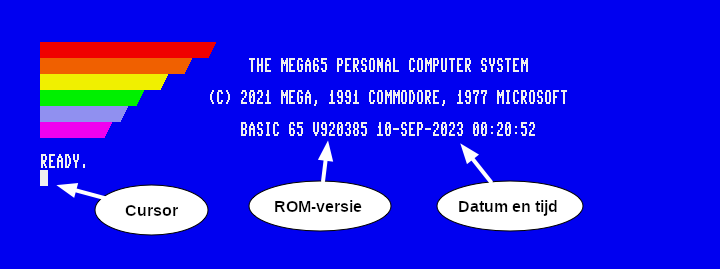
\includegraphics[width=0.9\linewidth]{dutch/images/introduction-screen/layout.png}
\end{center}

De kleurbalken linksboven in het scherm kunt u gebruiken als richtlijn om de kleuren van uw beeldscherm te kalibreren. Het scherm toont tevens de naam van het systeem, de copyrightmelding en de ROM-versie. De weergegeven datum en tijd zijn afkomstig van de interne RTC (Real-Time Clock) op het moment dat de computer werd ingeschakeld. U kunt de datum en tijd instellen in het configuratiehulpprogramma.

Ten slotte ziet u de \screentext{READY}-prompt en de knipperende cursor.

U kunt beginnen met typen op het toetsenbord en de tekens verschijnen op de cursorpositie. Na elke toetsaanslag schuift de cursor één positie verder.

U kunt ook omgekeerde tekst of kleurbalken maken door \specialkey{CTRL} ingedrukt te houden en \megakey{9} of \megakey{R} in te drukken. Hiermee schakelt u de modus voor omgekeerde tekst in. Indien deze modus is ingeschakeld, kunt u de spatiebalk \megakey{Space} indrukken en ingedrukt houden. Terwijl u dat doet, wordt een witte balk over het scherm getekend.
\index{Toetsenbord!CTRL}
U kunt de huidige kleur wijzigen door \specialkey{CTRL} ingedrukt te houden en een cijfertoets in te drukken (van \megakey{1} tot \megakey{8}). Indien u bijvoorbeeld \specialkey{CTRL} ingedrukt houdt en \megakey{1} indrukt, verandert de kleur in zwart. Wanneer u nu de spatiebalk \megakey{Space} ingedrukt houdt, wordt een zwarte balk getekend. Indien u de kleur blijft wijzigen en de spatiebalk \megakey{Space} indrukt, krijgt u een effect dat vergelijkbaar is met de volgende afbeelding:

\begin{center}
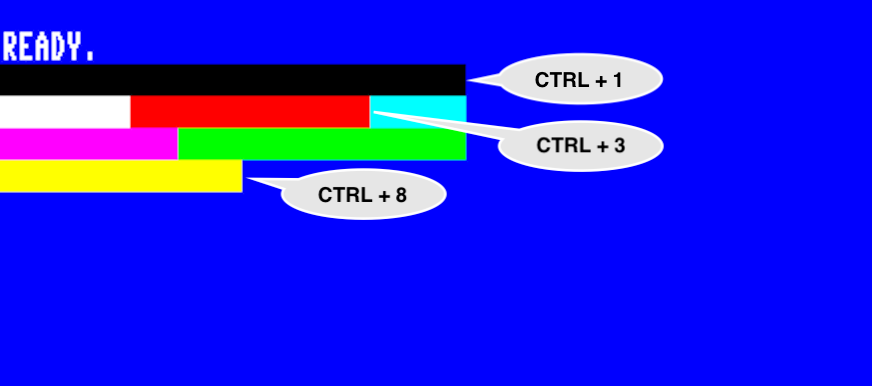
\includegraphics[width=0.7\linewidth]{images/introduction-screen/colour-bars.png}
\end{center}

U kunt de modus voor omgekeerde tekst uitschakelen door \specialkey{CTRL} ingedrukt te houden en \megakey{0} in te drukken.

Nog acht kleuren kunt u selecteren door \megasymbolkey ingedrukt te houden en een toets van \megakey{1} tot \megakey{8} in te drukken.\index{Toetsenbord!MEGA-toets}

De kleur die op de onderste rij aan de voorkant van de cijfertoets is afgedrukt, wordt gebruikt. Indien u bijvoorbeeld \megasymbolkey ingedrukt houdt terwijl u \megakey{4} indrukt, wordt donkergrijs gebruikt. Voor toegang tot nog 16 kleuren van het alternatieve/rainbow-palet verwijzen wij u naar de sneltoets \specialkey{CTRL} + \megakey{A}, die beschreven staat op bladzijde \pageref{appendix:controlcodes}.

\underline{OPMERKING}:
\begin{itemize}
  \item {\bf Zinnebeeldmodus}: Indien u \megakey{"} indrukt om een tekenreeks te beginnen en vervolgens probeert kleuren te wijzigen, tekst om te keren, de cursor te verplaatsen of de toets \specialkey{CLR\\HOME} te gebruiken, verschijnen er in plaats van dat deze acties onmiddellijk plaatsvinden, grappige PETSCII\index{PETSCII}-tekens. Dit komt door een voorziening van BASIC die {\it zinnebeeldmodus} heet en waarmee u dergelijke acties in een tekenreeks kunt coderen, zodat u ze op een later tijdstip kunt uitvoeren (bijvoorbeeld via een {\bf PRINT}-instructie in uw programma's). Om de zinnebeeldmodus te beëindigen typt u eenvoudig een nieuwe \megakey{"} om het einde van uw tekenreeks aan te geven.  \item {\bf Invoegmodus}: Een vergelijkbare voorziening is de {\it invoegmodus}. Het aantal keren dat u \specialkey{SHIFT} + \specialkey{INST\\DEL} indrukt om enkele spaties in te voegen, is gelijk aan het aantal toetsaanslagen dat erop volgt en dat zich volgens dezelfde beginselen als de zinnebeeldmodus gedraagt.  \item U kunt beide modi ook geforceerd beëindigen door \specialkey{ESC} en daarna \megakey{O} in te drukken.
\end{itemize}

\needspace{4cm}
U kunt eenvoudig leuke afbeeldingen maken door deze kleuren en letters te gebruiken. Hieronder ziet u een voorbeeld van wat een vierdejaarsstudent tekende:

\begin{center}
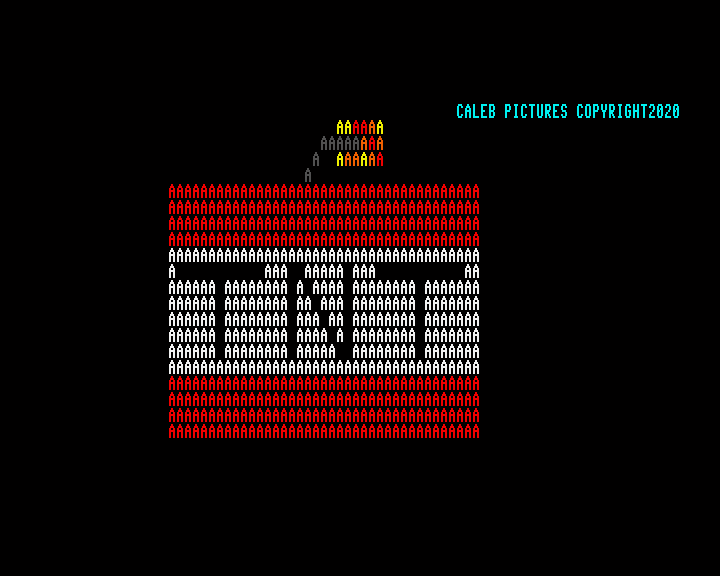
\includegraphics[width=0.7\linewidth]{images/caleb-PETSCII-TNT-final}
\end{center}

Wat gaat u tekenen?

\needspace{2cm}
\textbf{Functies}

Functies die gebruikmaken van \specialkey{CTRL} worden \textbf{Controlcodes} genoemd. Functies die gebruikmaken van \megasymbolkey worden \textbf{Megacodes} genoemd. Er bestaan ook functies die via \specialkey{SHIFT} worden aangeroepen; deze worden \textbf{Shiftcodes} genoemd.

Ten slotte maakt \specialkey{ESC} het gebruik van \textbf{escape-sequenties} mogelijk.

Over al deze functies leest u meer op bladzijde \pageref{appendix:controlcodes}.

\needspace{2cm}
\textbf{Escape-sequenties}

\index{Toetsenbord!Escape-reeksen}
Escape-sequenties worden iets anders uitgevoerd dan een controlcode of een shiftcode. In plaats van de modificatietoets ingedrukt te houden, voert u een escape-sequentie uit door \specialkey{ESC} in te drukken, deze los te laten en vervolgens de gewenste toets in te drukken.

Om bijvoorbeeld te schakelen tussen de 80-kolomsmodus en de 40-kolomsmodus drukt u \specialkey{ESC} in, laat u deze los en drukt u vervolgens op \megakey{X}.

Er zijn nog meer tekstmodi beschikbaar. U kunt knipperende tekst maken door \specialkey{CTRL} ingedrukt te houden en op \megakey{O} te drukken. Alle tekens die u intypt, zullen knipperen. Schakel de knippermodus uit door \specialkey{ESC} en daarna \megakey{O} in te drukken.


\section{Functionaliteit van de editor}

De schermeditor van de MEGA65\index{Schermeditor} biedt verschillende manieren om de cursor snel over het scherm te verplaatsen, zodat u productiever kunt werken.

Druk bijvoorbeeld op \specialkey{CLR\\HOME} om naar de startpositie op het scherm te gaan. Houd \specialkey{CTRL} ingedrukt en druk enkele malen op \megakey{W}. Dit is de functie \textbf{Word Advance}, die uw cursor naar het volgende woord of afdrukbare teken verplaatst.

U kunt naar eigen inzicht tabposities op het scherm instellen. Druk op \specialkey{CLR\\HOME} en vervolgens op \megakey{$\rightarrow$} om de cursor naar de vierde kolom te verplaatsen. Houd \specialkey{CTRL} ingedrukt en druk op \megakey{X} om een tab in te stellen. Verplaats de cursor nog 16 posities naar rechts en druk opnieuw op \specialkey{CTRL} en \megakey{X} om een tweede tab in te stellen.

Druk op \specialkey{CLR\\HOME} om terug te keren naar de startpositie. Houd \specialkey{CTRL} ingedrukt en druk op \megakey{I}. Dit is de functie \textbf{Forward Tab}. Uw cursor springt naar de vierde positie. Druk opnieuw op \specialkey{CTRL} en \megakey{I}. Uw cursor verplaatst zich naar positie 8. Standaard is elke achtste positie reeds als tabpositie ingesteld. De vierde en de twintigste positie zijn derhalve toegevoegd aan de bestaande tabposities. U kunt op \specialkey{CTRL} en \megakey{I} blijven drukken om door te springen naar de zestiende en twintigste positie.

\subsection{Een venster maken}
\index{Toetsenbord!Escape-reeksen}
\index{Vensters!Escape-reeksen}

U kunt een venster instellen op het werkscherm van de MEGA65. Verplaats uw cursor naar het begin van de tekst ``BASIC 65''. Druk op \specialkey{ESC} en daarna op \megakey{T}. Verplaats de cursor 10 regels omlaag en 15 posities naar rechts.

Druk op \specialkey{ESC} en daarna op \megakey{B}. Alles wat u typt, blijft binnen dit venster.

Indien u bijvoorbeeld \screentext{LIST} typt om een programma weer te geven, blijft de listing beperkt tot het venstergedeelte dat u hebt aangegeven:

\begin{center}
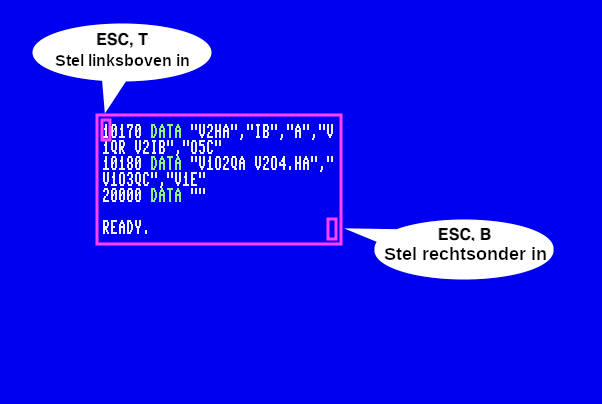
\includegraphics[width=0.7\linewidth]{dutch/images/set-window.png}
\end{center}

Druk tweemaal op \specialkey{CLR\\HOME} om het venster te verlaten en terug te keren naar het volledige scherm.

\subsection{Aanvullende ASCII-tekens}

U hebt misschien opgemerkt dat zich op het toetsenbord van de MEGA65 een aantal ASCII-tekens bevindt die van oudsher geen deel uitmaken van de PETSCII-tekenset\index{PETSCII}. Om deze tekens te gebruiken:

\begin{itemize}
  \item Typ \screentext{FONT A} of \screentext{FONT B}.  \item Druk op \megasymbolkey + \specialkey{SHIFT} om over te schakelen naar kleine letters.
\end{itemize}

U kunt die extra ASCII-tekens nu typen door \megasymbolkey ingedrukt te houden en de toets in te drukken.

\begin{center}
  \begin{tabular}{|l|c|l|}
  \hline
  \textbf{Naam} & \textbf{Teken} & \textbf{Toetscombinatie} \\
  \hline
  Backtick & \texttt{\`} & \megasymbolkey + \megakeywhite{$\leftarrow$} \\
  \hline
  Tilde & \texttt{\~} & \megasymbolkey + \megakey{,} (komma) \\
  \hline
  Verticale streep & \texttt{|} & \megasymbolkey + \megakey{.} (punt) \\
  \hline
  Backslash & \texttt{\textbackslash} & \megasymbolkey + \megakey{/} \\
  \hline
  Linker accolade & \texttt{\{} & \megasymbolkey + \megakey{:} \\
  \hline
  Rechter accolade & \texttt{\}} & \megasymbolkey + \megakey{;} \\
  \hline
  Underscore & \texttt{\_} & \megasymbolkey + \megakey{=} \\
  \hline
  \end{tabular}
\end{center}

De alternatieve lettertypen vervangen tekens uit de oorspronkelijke PETSCII-tekenset door deze symbolen. Om terug te keren naar de PETSCII-tekenset, typt u \screentext{FONT C}.

\subsection{Hoofdletters en kleine letters}

\megasymbolkey + \specialkey{SHIFT} schakelt voor het volledige scherm tussen tekst in hoofdletters en tekst in kleine letters. Dit werkt ook tijdens de uitvoering van een programma, zodat u het kunt aanpassen wanneer een programma zich in de verkeerde modus bevindt.


\section{Het Freezer-menu}
\label{sec:freezer}
\index{Freezer-menu}
\nopagebreak
De MEGA65 brengt het grootste deel van zijn tijd door als een Commodore 65-computer, door een programma uit te voeren of te wachten op instructies in de BASIC-omgeving. Uw MEGA65 beschikt over extra voorzieningen die geen deel uitmaakten van het oorspronkelijke C65-ontwerp. U hebt toegang tot veel van deze voorzieningen via het Freezer-menu.

Om het Freezer-menu te openen, houdt u de toets \widekey{RESTORE} één seconde ingedrukt en laat u deze vervolgens los. De MEGA65 onderbreekt zijn bezigheden, laat de randkleur flikkeren en opent vervolgens het Freezer-menu. Het programma dat op dat moment liep, blijft in het geheugen staan en kan worden hervat door op de toets \megakey{F3} te drukken. U kunt het draaiende programma ook afbreken en de MEGA65 resetten door op \megakey{F5} te drukken.

\begin{center}
  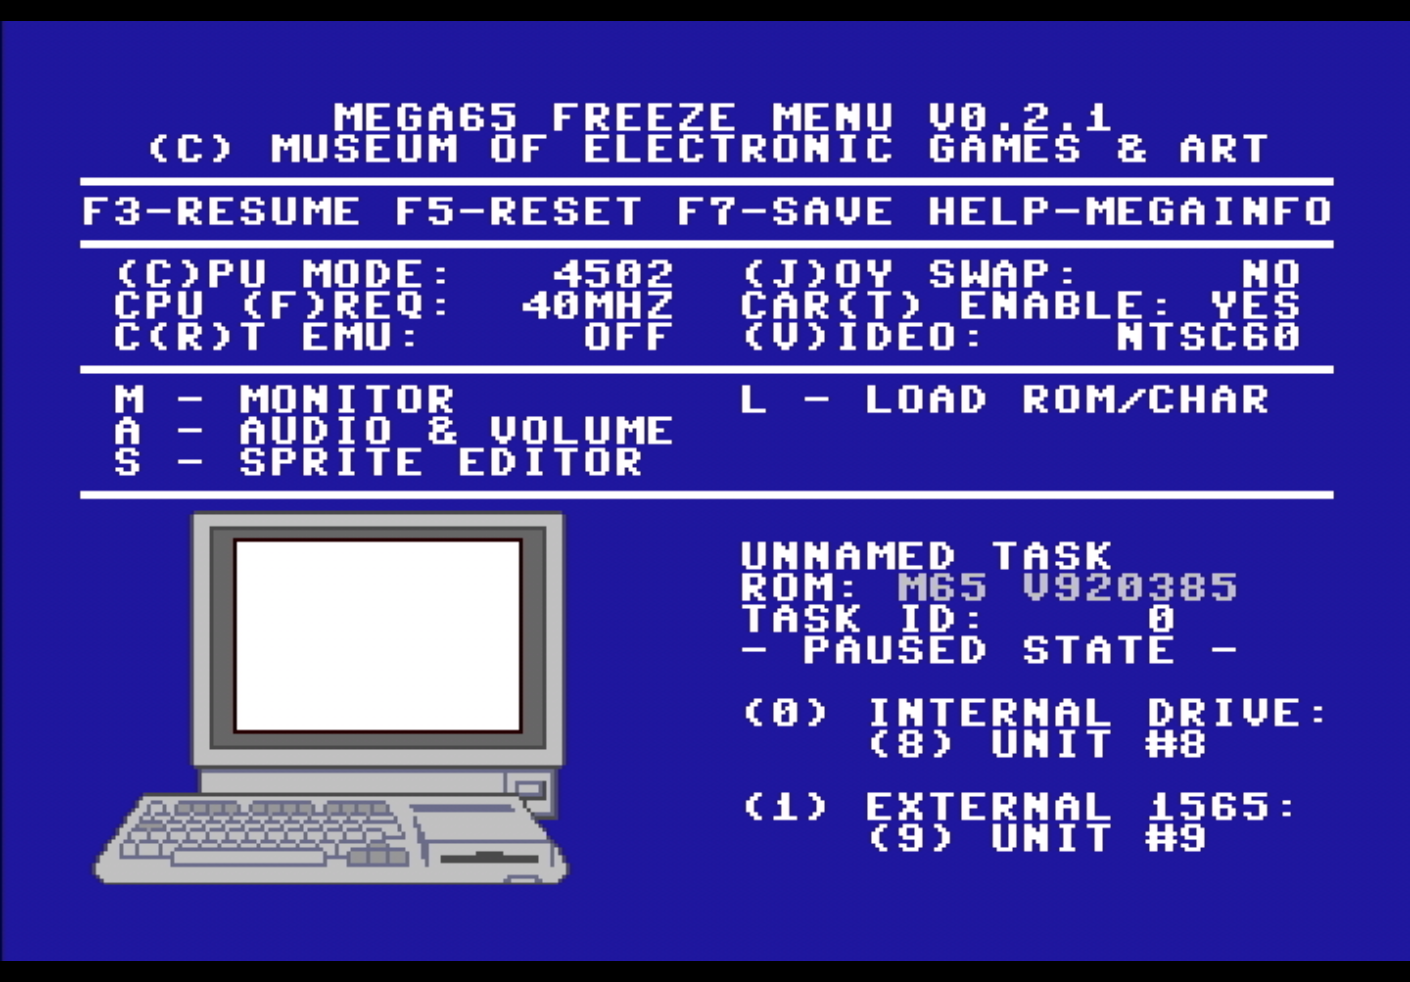
\includegraphics[width=0.7\linewidth]{images/freezer.png}
\end{center}

Een functie om te onthouden tijdens het spelen van spellen is ``(J)OY SWAP''. Deze functie laat de joystickpoorten van nummer wisselen. Hebt u een joystick in poort 2 en start u een spel dat een joystick in poort 1 verwacht, dan hoeft u de joystick niet los te koppelen en opnieuw aan te sluiten. Open in plaats daarvan het Freezer-menu, druk op \megakey{J} om de poortnummers om te wisselen en hervat vervolgens uw spel.

Het menu wordt ``Freezer'' genoemd omdat de toestand van de MEGA65 bevroren blijft terwijl u het menu gebruikt. Het Freezer-menu kan meerdere freeze-toestanden opslaan en u kunt tussen deze toestanden schakelen. Om de huidige toestand op te slaan, gaat u met de rechtercursortoets naar een ongebruikt {\it freeze-slot} en drukt u vervolgens op \megakey{F7}. Wanneer de rand ophoudt met knipperen, is de toestand opgeslagen. Om een toestand te herstellen, gaat u naar het freeze-slot en drukt u op \megakey{F3} om de werking te hervatten.

Het Freezer-menu bevat diverse ingebouwde opties en voorzieningen. Zie voor meer informatie over het MEGA65-informatiehulpprogramma (``MEGAINFO'') ``De versies van de onderdelen bepalen'' op bladzijde \pageref{sec:versions}. Zie voor meer informatie over het aankoppelen van schijven en schijfimages hoofdstuk \vref{cha:using-disks}.


\section{Commodore 64-software uitvoeren}

De MEGA65 is in staat Commodore 64-software uit te voeren. Hiervoor zijn twee mogelijkheden: de ingebouwde GO64-modus en de FPGA-core {\it C64 for MEGA65}.

\subsection{GO64-modus}
\index{Commodore 64!GO64-modus}

De oorspronkelijke Commodore 65 was ontworpen om bepaalde Commodore 64-software te kunnen uitvoeren. De MEGA65 ondersteunt deze voorziening, die bekendstaat als ``GO64-modus''.

\underline{OPMERKING}: Doordat Commodore deze voorziening op deze wijze heeft ontworpen, is niet alle C64-software compatibel met deze modus. Anders dan de vergelijkbare voorziening van de Commodore 128 gebruikt de Commodore 65 een andere CPU en het is bekend dat kleine verschillen compatibiliteitsproblemen met sommige softwaretitels veroorzaken.

Er zijn drie manieren om de MEGA65 in de GO64-modus te schakelen:

\begin{itemize}
    \item Schakel de computer uit, houd de \megasymbolkey ingedrukt en schakel hem weer in.    \item Geef bij de \screentext{READY}-prompt van de MEGA65 dit commando in: \screentext{GO64} en druk op Enter. Typ \screentext{YES} wanneer daarom wordt gevraagd.\index{BASIC 65-commando's!GO64}    \item Schakel de computer uit, sluit een Commodore 64-cartridge aan op de expansiepoort en schakel de computer vervolgens weer in.
\end{itemize}

\begin{center}
  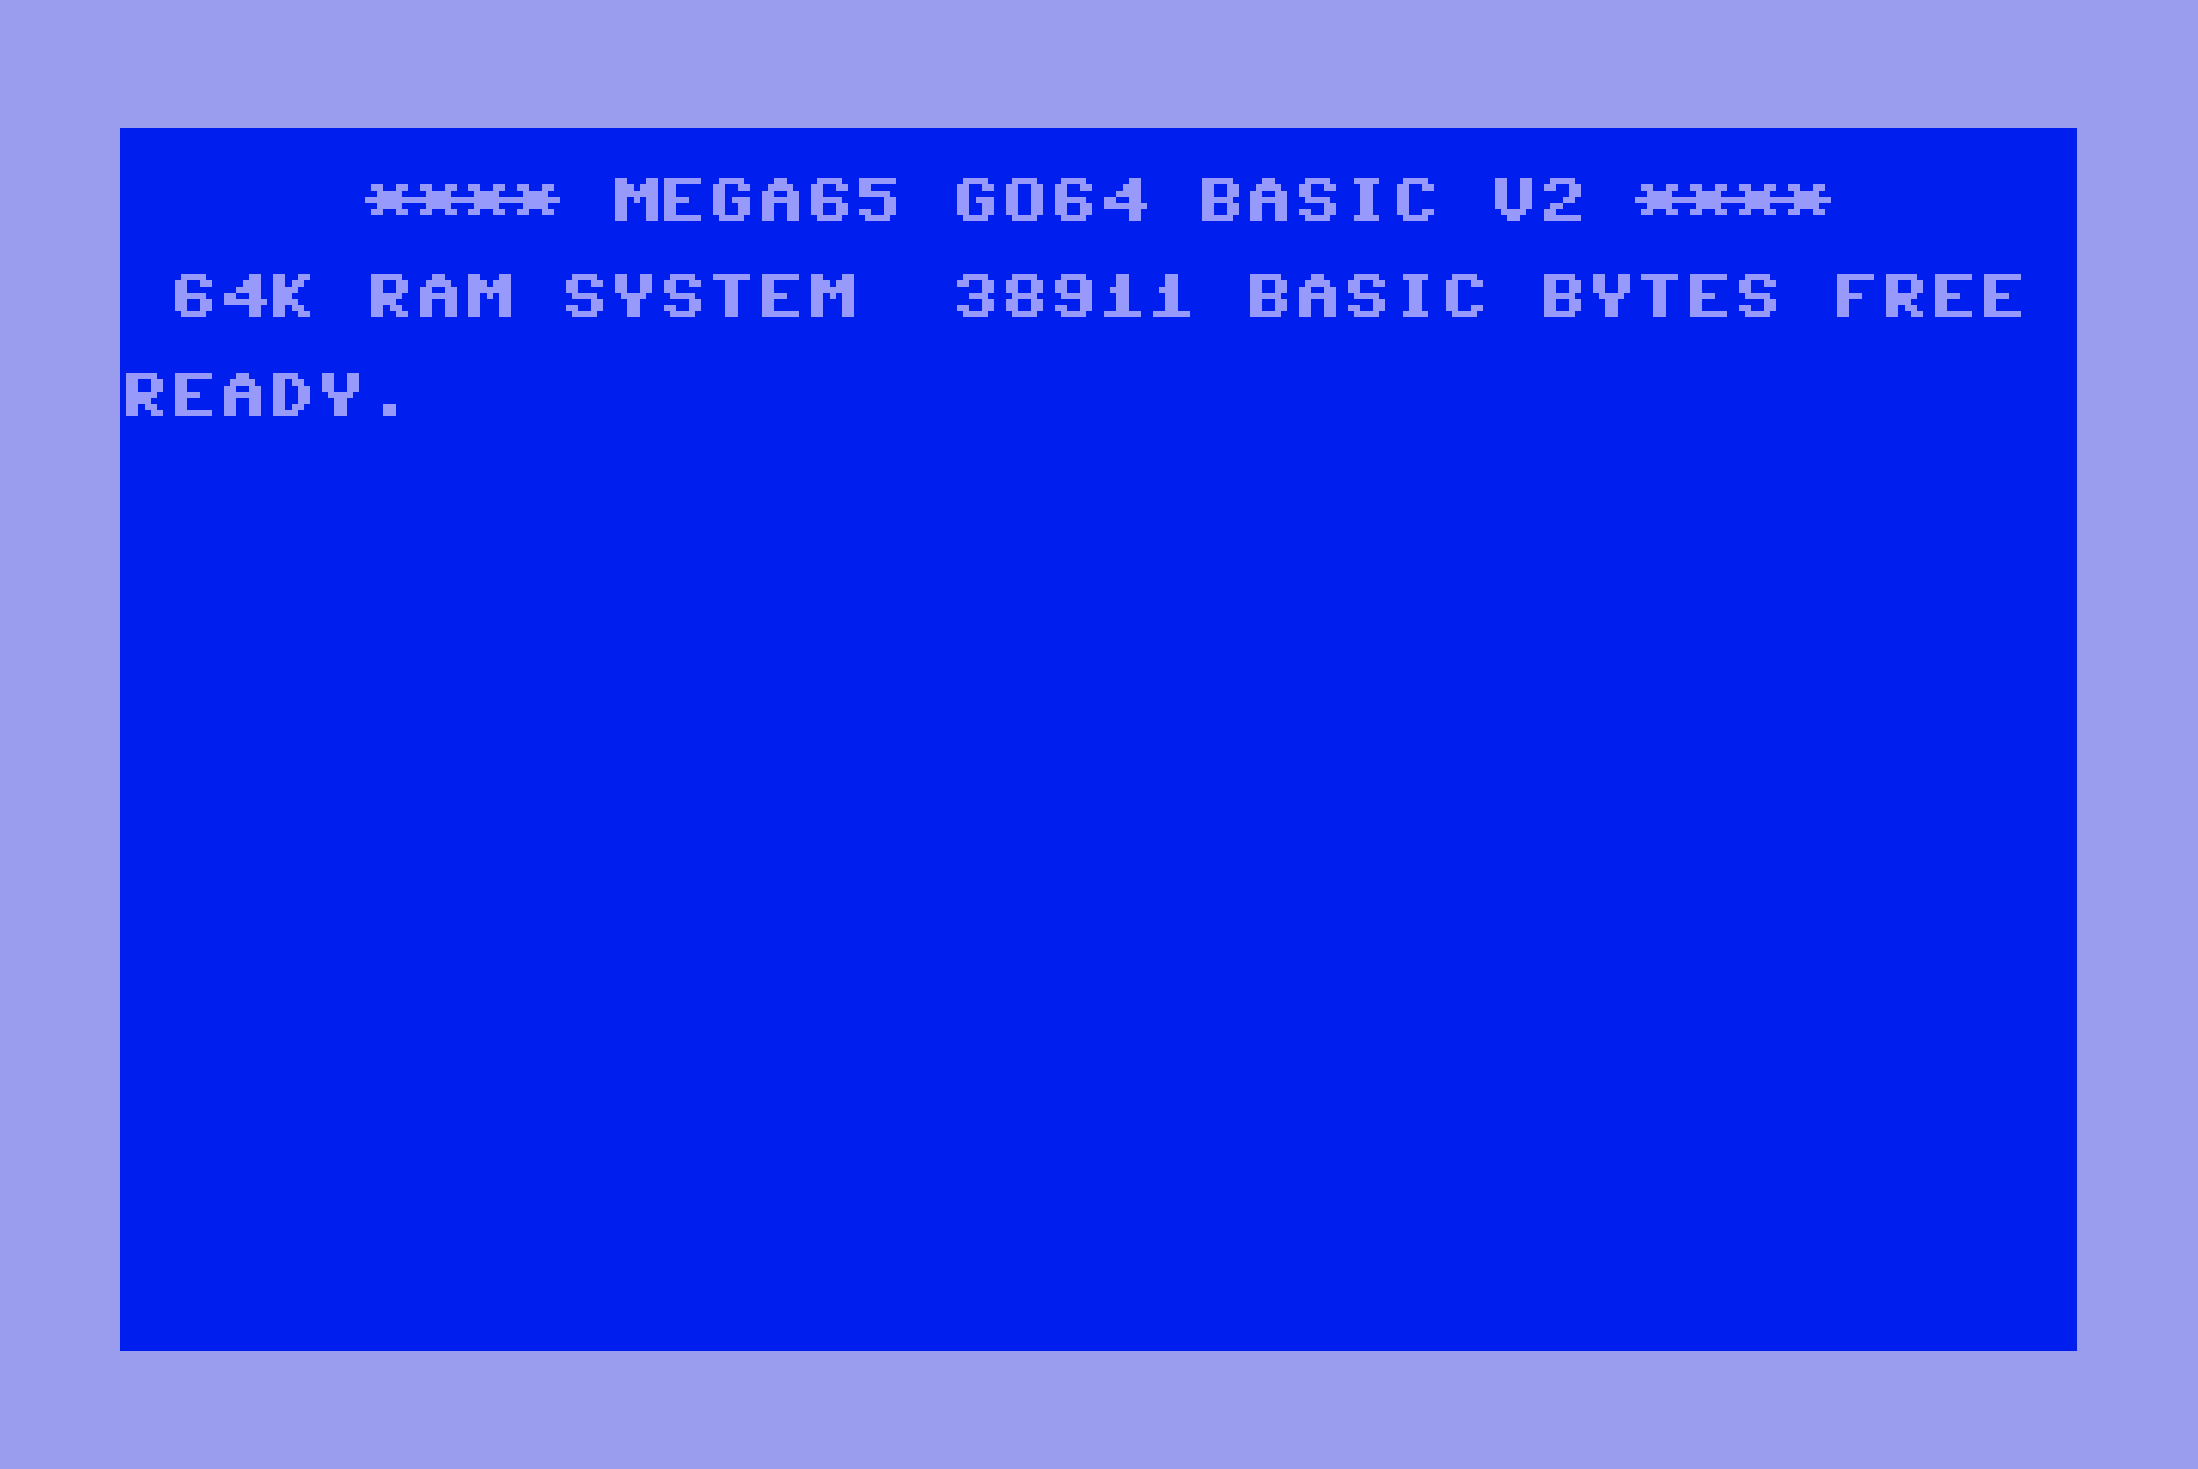
\includegraphics[width=0.7\linewidth]{images/go64.pdf}
\end{center}

De GO64-modus is eigenlijk slechts een tijdelijke herconfiguratie van de MEGA65. Alle voorzieningen van de MEGA65 blijven aanwezig, waaronder het Freezer-menu voor het aankoppelen van D81-schijfimages.

Veel Commodore 64-software is op het internet te vinden in de vorm van D64-schijfimages. De MEGA65 ondersteunt via de SD-kaart en het Freezer-menu uitsluitend D81-schijfimages. U kunt een randapparaat, zoals de SD2IEC,\index{SD2IEC device} op de IEC-poort van de MEGA65 aansluiten om D64-schijfimages te gebruiken. Zorg dat u een SD2IEC aanschaft met een onafhankelijke voeding en niet een exemplaar dat afhankelijk is van een tape-aansluiting van de Commodore 64.\footnote{Zie voor meer informatie over SD2IEC-apparaten: \url{https://www.c64-wiki.com/wiki/SD2IEC}}

\subsection{De FPGA-core ``C64 for MEGA65''}
\index{Core!C64-core}\index{Commodore 64!Core}

De FPGA-core {\it C64 for MEGA65} van MJoergen en sy2002 herschept de oorspronkelijke Commodore 64-computer op de MEGA65-hardware met een hoge mate van nauwkeurigheid. Het doet dit door de MEGA65-core volledig te vervangen door een core die de chipset van de Commodore 64 implementeert, met inbegrip van de CPU. MEGA65-voorzieningen, zoals het Freezer-menu, zijn niet beschikbaar wanneer de C64-core draait. In plaats daarvan biedt de core een eigen menu voor het aankoppelen van D64-schijfimages en andere voorzieningen. Druk op de toets \specialkey{HELP} terwijl de core draait om dit menu te openen.

% TODO: When the cartridge-to-core configuration feature is complete:
% With the C64 core installed, you can configure the MEGA65 boot process to use the core when a Commodore 64 cartridge is connected, instead of using the less-compatible GO64 mode. ...
% (Refer to chapter \vref{cha:cores})

Zie voor informatie over het installeren van FPGA-cores hoofdstuk \vref{cha:cores}. Om de core {\it C64 for MEGA65} te downloaden en de belangrijke installatie-instructies te lezen, zie: \url{https://github.com/MJoergen/C64MEGA65}

\chapter{Configureren van uw MEGA65}

\section{Configureren van uw MEGA65}
\label{cha:configuringyourmega}
\index{Configuratie}

Dit hoofdstuk beschrijft hoe u uw MEGA65 configureert.

Omdat de configuratiegegevens op de SD-kaart worden opgeslagen, beschrijft dit hoofdstuk ook hoe u een nieuwe SD-kaart voorbereidt. Uw MEGA65 wordt met een vooraf geïnstalleerde SD-kaart geleverd. Indien u uw MEGA65 met de vooraf geïnstalleerde SD-kaart configureert en later een nieuwe SD- of microSD-kaart installeert, moet u uw configuratie-instellingen opnieuw instellen.

Dit hoofdstuk laat u tevens kennismaken met de website MEGA65 Filehost, waarmee u games, apps, hulpprogramma's en systeemupdates voor uw computer kunt downloaden.

\section{Configuratiehulpprogramma}
\label{sec:configuration-utility}
\index{Configuratie!Hulpprogramma}

U kunt uw MEGA65 configureren met het Configuratiehulpprogramma. Dit omvat de instellingen die werden weergegeven toen u de computer voor het eerst inschakelde en vele andere.

Om het Configuratiehulpprogramma te openen, schakelt u de MEGA65 uit, houdt u de toets \specialkey{ALT} ingedrukt en schakelt u de MEGA65 weer in. Het hulpprogrammamenu\index{Hulpprogrammamenu} verschijnt met verschillende opties. Druk op \megakey{1} om het Configuratiehulpprogramma te starten.

\begin{center}
  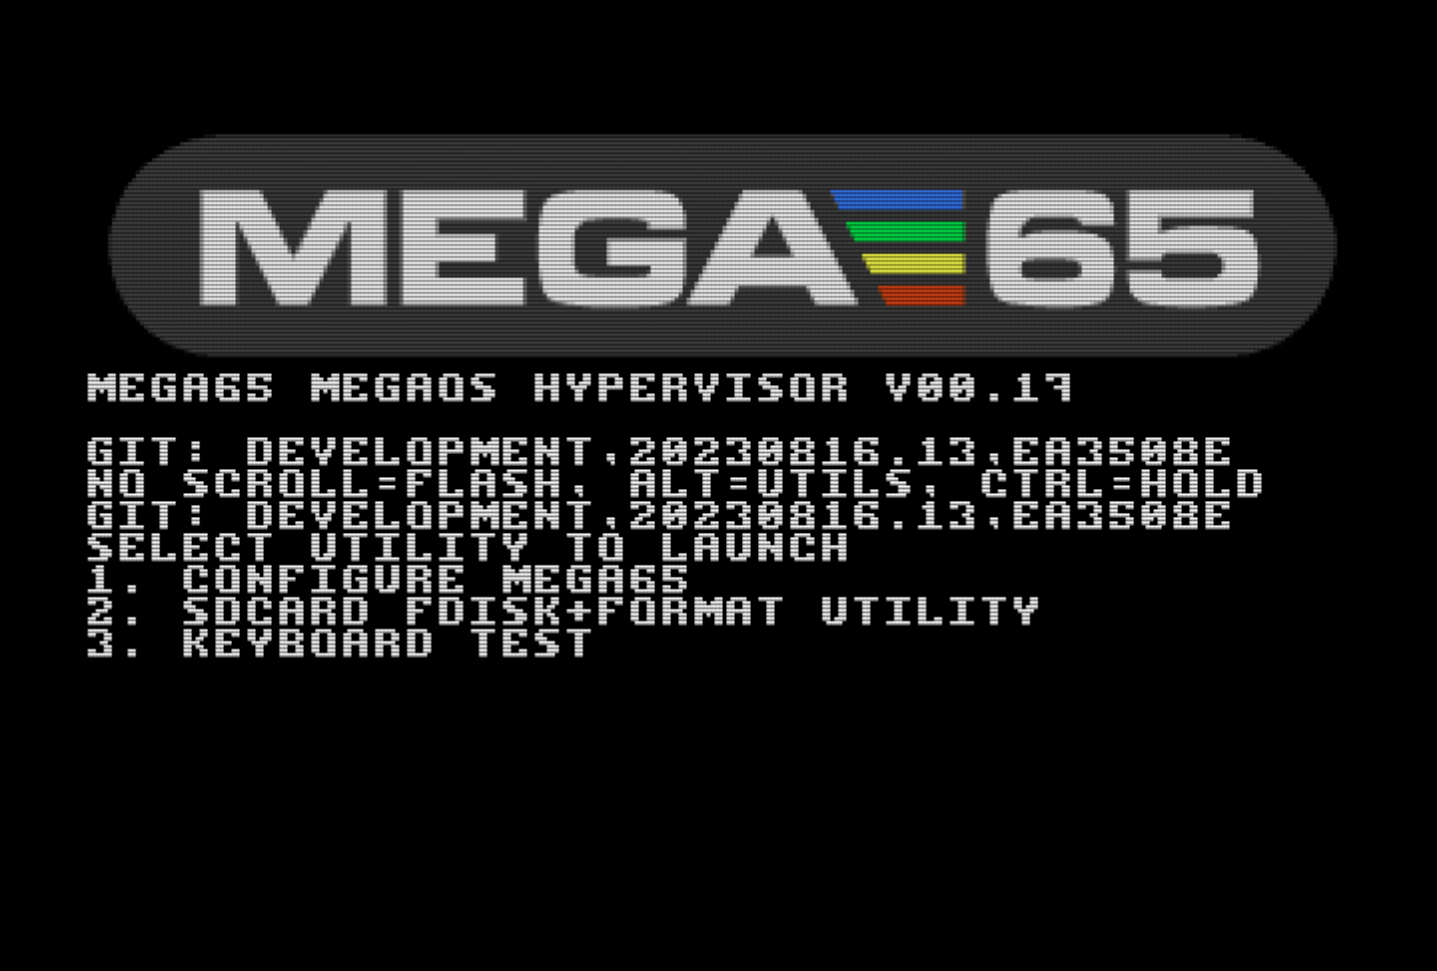
\includegraphics[width=0.7\linewidth]{images/ss-utilmenu.png}
\end{center}

Het Configuratiehulpprogramma bevat verscheidene bladzijden met instellingen, die u kunt doorlopen met het toetsenbord of met een op poort 1 aangesloten muis. Gebruik \megakey{$\leftarrow$} en \megakey{$\rightarrow$} om tussen de bladzijden te bladeren en \megakey{$\uparrow$} en \megakey{$\downarrow$} om onderdelen op een bladzijde te selecteren. Druk op \specialkey{RETURN} of \megakey{SPACE} om een instelling om te schakelen of een waarde te wijzigen.

\subsection{Input}
\index{Configuratie!Muis}

Op de bladzijde {\bf Input} stelt u de muisinstellingen voor de twee randapparaatpoorten in.

\begin{center}
  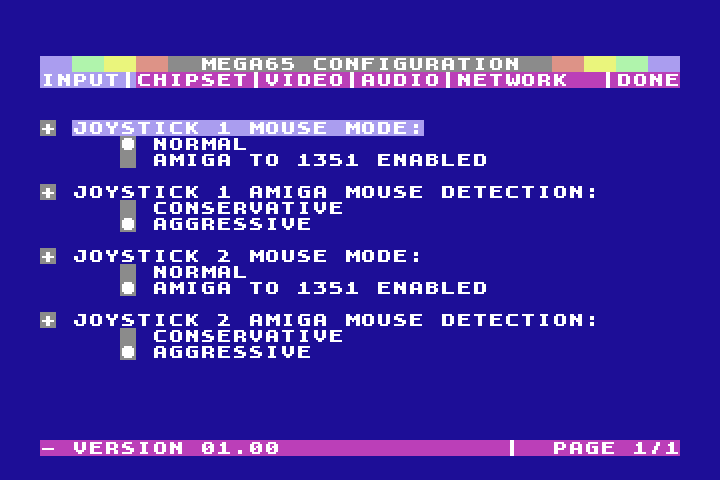
\includegraphics[width=0.7\linewidth]{images/ss-m65config-1.png}
\end{center}

De MEGA65 ondersteunt de Commodore 1351-muis,\index{Commodore 1351-muis} de Commodore Amiga-muis\index{Commodore Amiga-muis} of moderne equivalenten, zoals een USB-muis die met een \href{https://retrohax.net/shop/amiga/mouster/}{mouSTer}-adapter is aangesloten.\index{mouSTer-adapter} De poort moet op het juiste muistype worden ingesteld, waarbij {\bf normal} naar de 1351-muis verwijst. Indien een Amiga-muis is aangesloten terwijl de poort in de modus {\bf normal} staat, kan deze het gedrag van het toetsenbord verstoren.

Met de instelling {\bf 1351 De-jitter} stelt u de gevoeligheid in de Commodore 1351-muismodus af om jitter van het muispijltje te voorkomen. Het wordt aanbevolen deze op {\bf on} te laten staan wanneer u in de modus {\bf normal} een 1351-muis gebruikt.

\subsection{Chipset}
\index{Configuratie!Opstartschijf}

Op de bladzijde {\bf Chipset} stelt u verschillende functies in, waaronder de real-time klok.

\begin{center}
  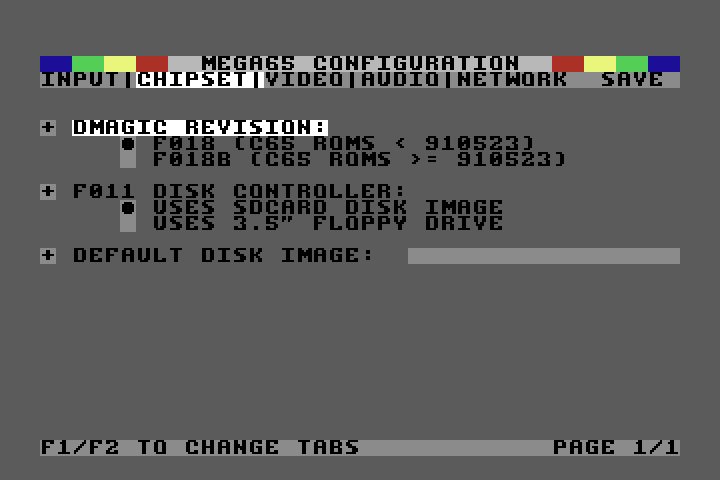
\includegraphics[width=0.7\linewidth]{images/ss-m65config-2.png}
\end{center}

Om de real-time klok in te stellen, selecteert u het tijd- of datumveld, typt u de volledige waarde en drukt u vervolgens op \specialkey{RETURN}.\index{Real-time klok!Datum/tijd instellen}\index{Configuratie!Real-time klok} De klokinstelling wordt pas van kracht wanneer u op \specialkey{RETURN} drukt; zonder \specialkey{RETURN} wijzigt er niets. Merk op dat alle overige instellingen pas aan het einde worden opgeslagen. Alleen de RTC wordt onmiddellijk bijgewerkt.

Het veld {\bf DMAGIC revision} bepaalt het gedrag van de DMA-controller. In de meeste gevallen wilt u de nieuwere instelling {\bf F018B} gebruiken. De instelling {\bf F018} dient voor achterwaartse compatibiliteit wanneer de C65-versies van de ROM worden gebruikt en is niet altijd vereist.

Het veld {\bf F011 disk controller}\index{F011-schijfcontroller} bepaalt of de MEGA65 bij het inschakelen van de computer een opstartschijf zoekt op de SD-kaart of in het fysieke 3.5 inch-diskettestation.\index{Configuratie!Opstartschijf} Wanneer deze op {\bf SDCARD disk image,} is ingesteld, gebruikt de MEGA65 het virtuele D81-schijfimage dat in het veld {\bf default disk image} is vermeld als opstartschijf. Wanneer u uw MEGA65 voor het eerst ontvangt, is dit ingesteld op de Intro Disk,\index{Intro Disk} genaamd {\tt MEGA65.D81}. U kunt dit wijzigen naar een andere schijf. Om het automatisch koppelen uit te schakelen, wijzigt u de schijfnaam in een bestandsnaam die niet bestaat, of hernoemt u het bestand {\tt MEGA65.D81} op de SD-kaart. (Indien u het veld leeg laat, wordt standaard {\tt MEGA65.D81} gebruikt.)

Indien {\bf F011 disk controller} op {\bf 3.5" floppy drive,} is ingesteld, pauzeert het opstartproces vlak vóór de \screentext{READY}-prompt om te controleren of er een opstartschijf in het station is geplaatst. Indien u geen fysieke opstartschijf gebruikt, kunt u deze op {\bf SDCARD disk image} laten staan voor een sneller opstartproces.

{\bf Long FN support} verwijst naar de ondersteuning van lange bestandsnamen in de bestandsbrowser van de MEGA65 voor SD-kaarten. Laat deze functie ingeschakeld, tenzij er problemen optreden bij het lezen van bestanden met bestandsnamen die langer zijn dan 11 tekens.

\subsection{Video}
\index{Configuratie!Video}

Op de bladzijde {\bf Video} stelt u de video-instellingen in. Dit zijn dezelfde instellingen als die van de initiële configuratie (``on-boarding''), waaronder de PAL- of NTSC-videomodus, het Digital Video-geluid en CRT-emulatie.\index{Configuratie!Introductie}\index{Scherm!PAL/NTSC instellen}

\begin{center}
  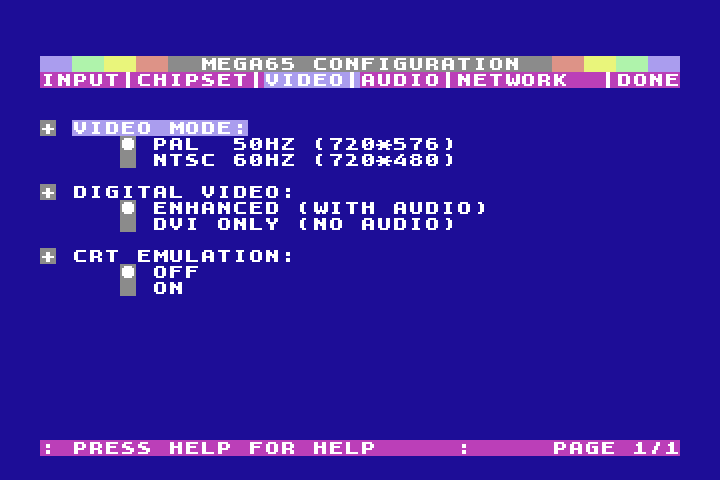
\includegraphics[width=0.7\linewidth]{images/ss-m65config-3.png}
\end{center}

Met {\bf Video mode} kiest u tussen de PAL-compatibiliteitsmodus en de NTSC-compatibiliteitsmodus. U kunt deze instelling ook tijdens het uitvoeren van programma's wijzigen met het Freezer-menu.

Met de instelling {\bf Digital Video} schakelt u het gecombineerde video- en audiosignaal over de Digital Video-poort in of uit. Indien uw Digital Video-beeldscherm ingebouwde luidsprekers heeft, schakelt u deze instelling in ({\bf Enhanced (with audio)}) om deze te gebruiken. Sommige DVI-beeldschermen zonder ingebouwde luidsprekers vereisen dat deze instelling wordt uitgeschakeld.

{\bf CRT emulation} is een optionele instelling die het beeld meer laat lijken op dat van een klassiek beeldbuismonitor wanneer u een modern plat beeldscherm gebruikt.

\subsection{Audio}
\index{Configuratie!Audio}

Op de bladzijde {\bf Audio} stelt u het geluidssysteem van de MEGA65 in.\index{Configuratie!Audio} In de meeste gevallen kunt u deze instellingen op hun standaardwaarden laten staan.

\begin{center}
  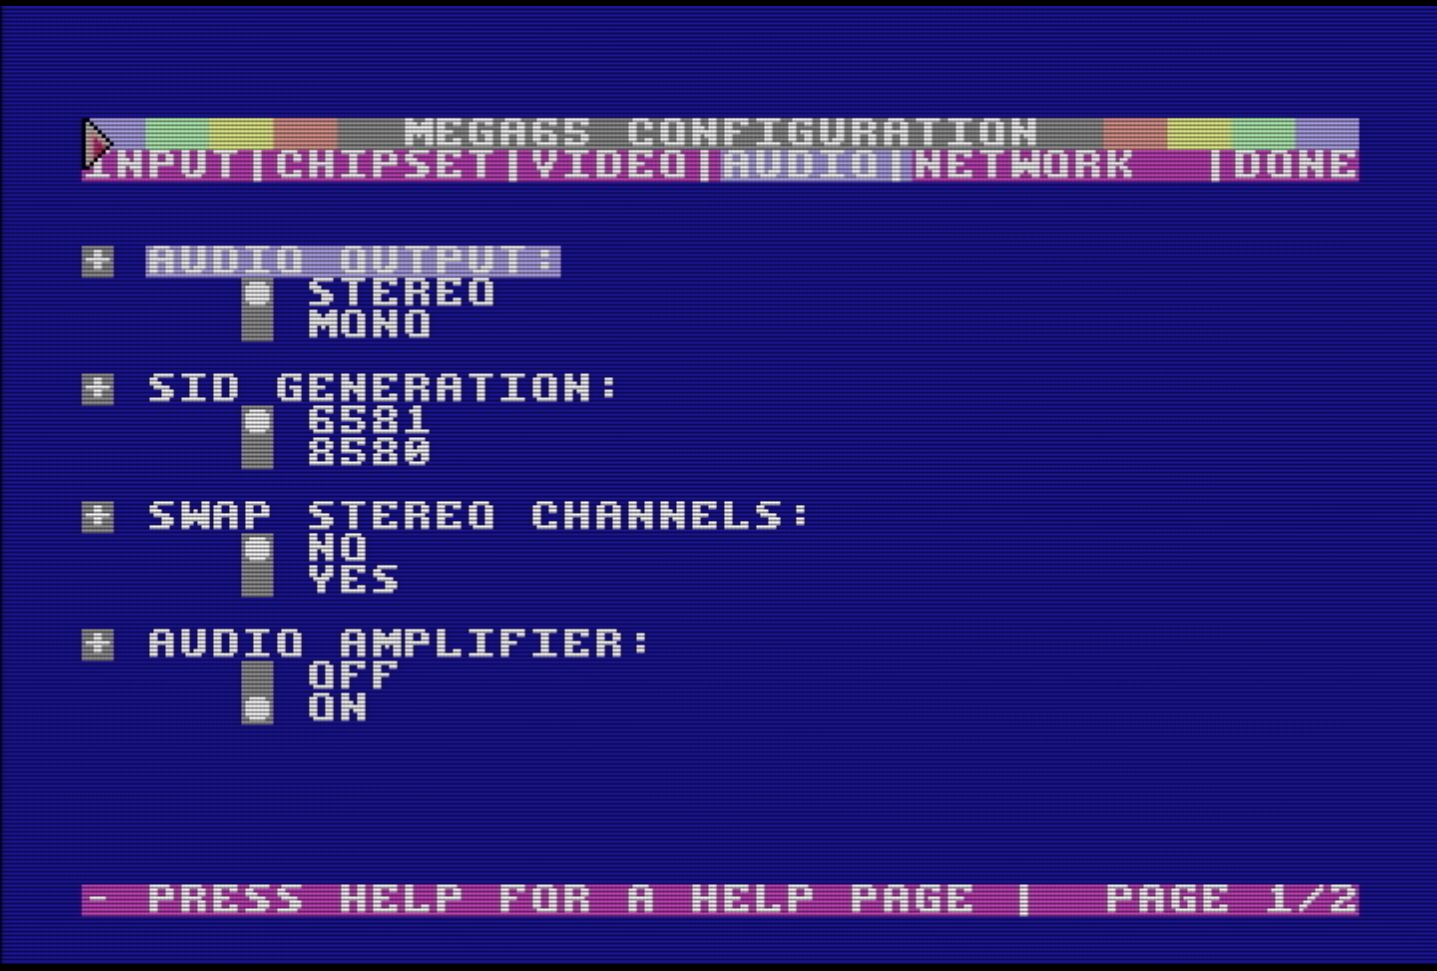
\includegraphics[width=0.7\linewidth]{images/ss-m65config-4.png}
\end{center}

{\bf Audio output} kan worden ingesteld op volledige stereo of op het verzenden van een monauraal signaal naar beide luidsprekers. In de stereomodus kunt u de diverse audioapparaten van de MEGA65 met de audiomixer in het Freezer-menu naar links of rechts in het stereobeeld verplaatsen. De standaardinstellingen plaatsen de vier SID-chips enigszins naar links en rechts.

{\bf SID generation} kiest tussen de audio-emulatie van de twee modellen SID-geluidschips: de oorspronkelijke 6581 die in sommige Commodore 64's wordt gebruikt en de nieuwere 8580 die in latere Commodore 64's en 128's wordt gebruikt. Sommige Commodore 64-spellen maakten gebruik van gebreken in de 6581 die in de 8580 zijn opgelost en klinken daardoor beter met de oudere generatie.

{\bf Swap stereo channels} laat de linker- en rechterluidsprekers van elkaar verwisselen.

{\bf Audio amplifier} regelt de ingebouwde versterker op de 3.5 mm-audioaansluiting. Stel deze in op {\bf on} wanneer u een hoofdtelefoon of een ander apparaat gebruikt dat een versterkt signaal verwacht. Stel deze in op {\bf off} voor een signaal op lijnniveau.

\subsection{Network}
\index{Configuratie!Netwerk}

Op de bladzijde {\bf Network} kunt u het MAC-adres van de ethernetpoort aanpassen. De MEGA65 heeft geen door de hardware toegewezen MAC-adres. In plaats daarvan gebruikt de computer de hier ingevoerde waarde.

Indien het MAC-adres geheel uit nullen bestaat, drukt u op de toets \megakey{R} om een willekeurig adres te genereren. Met een MAC-adres dat geheel uit nullen bestaat, werken netwerkfuncties niet.\index{Configuratie!MAC-adres}\index{Netwerk!MAC-adres}

\begin{center}
  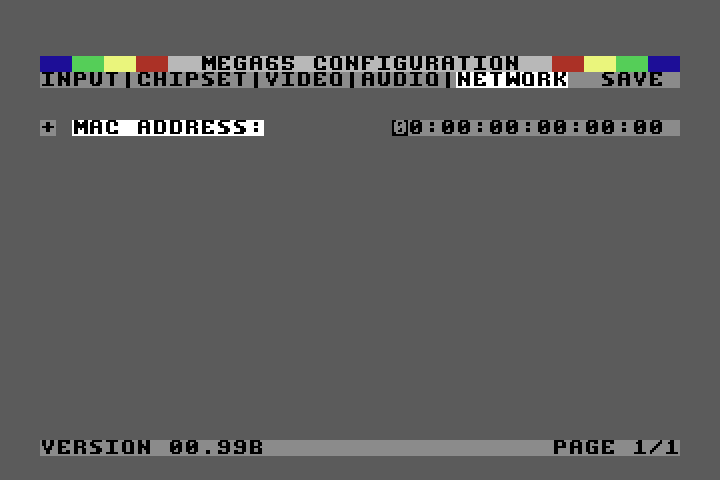
\includegraphics[width=0.7\linewidth]{images/ss-m65config-5.png}
\end{center}

\subsection{Done}

Op de bladzijde {\bf Done} kunt u het Configuratiehulpprogramma verlaten. Indien u wijzigingen hebt aangebracht die u wilt behouden, selecteert u {\bf Save as defaults and exit.} U kunt de wijzigingen ook verwerpen, de fabrieksinstellingen herstellen of volledig opnieuw opstarten naar het scherm van de initiële configuratie.

\begin{center}
  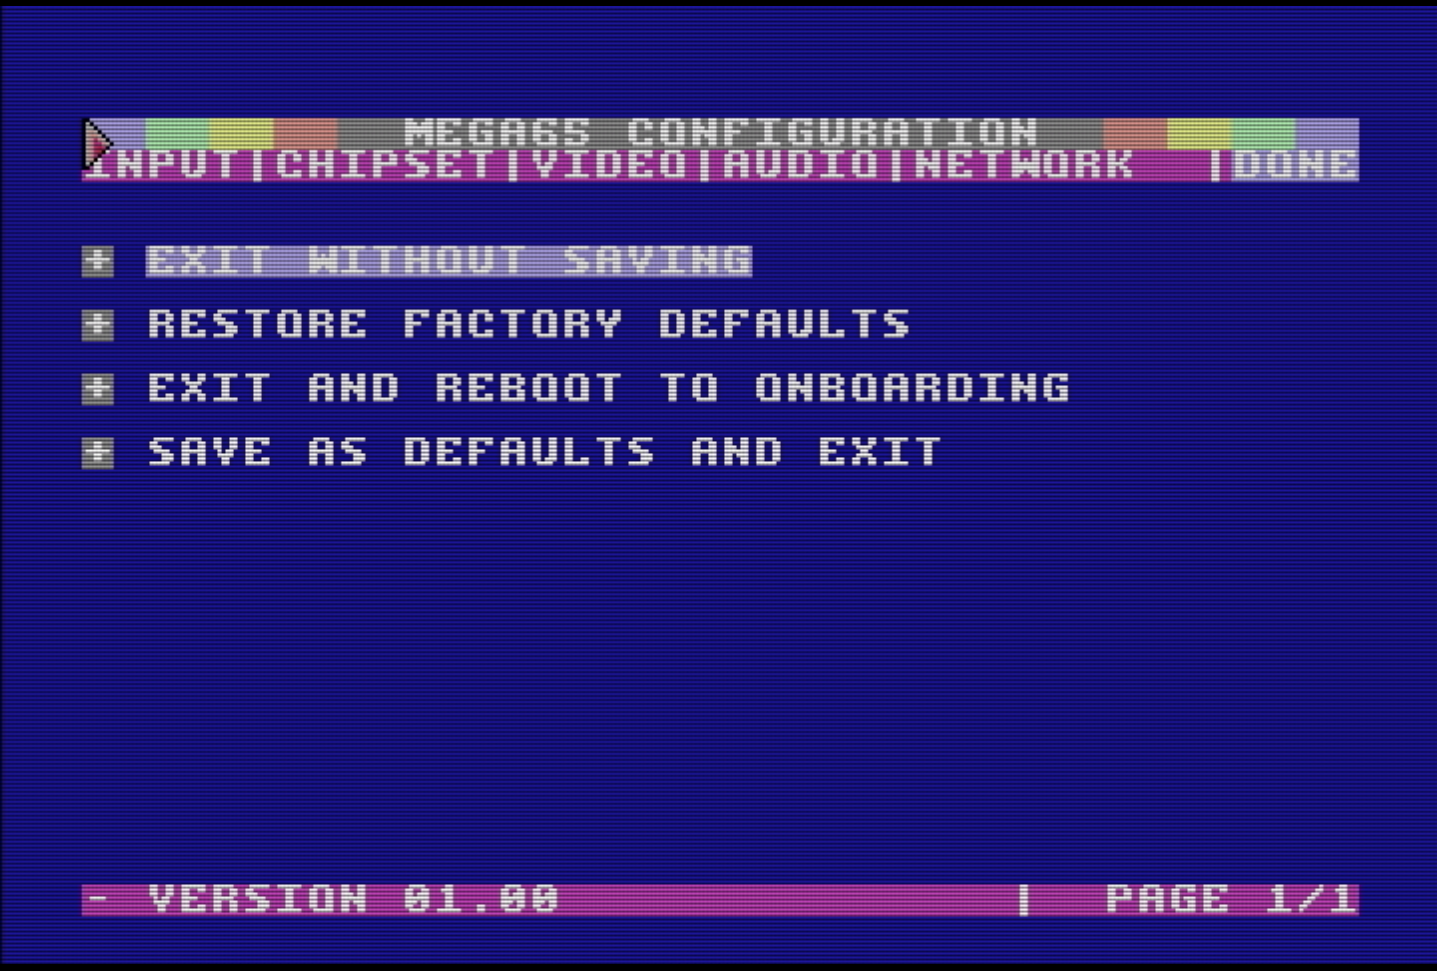
\includegraphics[width=0.7\linewidth]{images/ss-m65config-save.png}
\end{center}

Wanneer u het Configuratiehulpprogramma verlaat, wordt u gevraagd de computer uit en weer in te schakelen. Schakel de computer uit en vervolgens weer in.

\section{Kennismaken met SD-kaarten}
\label{sec:introducing-sd-cards}
\index{SD-kaarten}
\nopagebreak
Uw MEGA65 is uitgerust met twee SD-kaartsleuven: een SD-kaartsleuf op vol formaat in de behuizing, bereikbaar via de onderzijde van de computer, en een microSD-kaartsleuf aan de achterzijde van de computer.\index{SD-kaarten!Locaties} De MEGA65 gebruikt de SD-kaart voor het opslaan van configuratie-instellingen, het laden van het besturingssysteem, het bijwerken van de firmware en het opslaan van uw programmatuur en gegevens als virtuele schijfimages.

De MEGA65 wordt geleverd met een SD-kaart op vol formaat in de interne SD-kaartsleuf, vooraf gevuld met de bestanden van het besturingssysteem en de meegeleverde programmatuur.\footnote{U kunt de oorspronkelijke inhoud van de SD-kaart opnieuw aanmaken met bestanden die u van het internet kunt downloaden. Desondanks wilt u wellicht een reservekopie van de inhoud van de SD-kaart op uw PC maken.} U kunt uw MEGA65 aansluiten en er direct mee beginnen, zonder een nieuwe SD-kaart in te stellen. U kunt deze SD-kaart op zijn plaats laten en doen alsof hij er niet is, alsof uw MEGA65 een computer uit de jaren negentig is met een verborgen mogelijkheid om niet-vluchtige gegevens op te slaan.

De MEGA65 gebruikt slechts één van de twee SD-kaartsleuven tegelijk. Indien er een microSD-kaart in de sleuf aan de achterzijde zit, wordt de interne SD-kaart genegeerd. Welke sleuf u gebruikt, hangt af van het beoogde gebruik van de computer. Naarmate u meer vertrouwd raakt met uw MEGA65, wilt u de SD-kaart wellicht tussen de MEGA65 en uw PC verplaatsen om bestanden te kopiëren en systeemupdates uit te voeren. Dit is gemakkelijker met de externe microSD-kaartsleuf.

U kunt uw MEGA65 ook met een ethernetkabel op uw PC of het plaatselijke netwerk aansluiten en met een hulpprogramma bestanden tussen de twee computers overbrengen. De bestandsoverdrachtfunctie heeft toegang tot de bestanden op de SD-kaart en gebruikt de sleuf die op dat moment actief is. Zie voor meer informatie over het overbrengen van bestanden hoofdstuk \vref{cha:transferring-files}.

\section{Een nieuwe SD-kaart voorbereiden}

U kunt de microSD-kaartsleuf aan de achterzijde van de MEGA65 gebruiken als permanente opslagruimte voor de configuratie- en systeembestanden van de computer. Een voorbereide kaart in deze sleuf heeft voorrang op de SD-kaart die in de computer is geïnstalleerd. Het is handig om een microSD-kaart geïnstalleerd te hebben indien u de kaart tussen uw MEGA65 en uw PC wilt verplaatsen.

De volgende aanwijzingen gelden voor geheugenkaarten in zowel de externe microSD-kaartsleuf als de interne SD-kaartsleuf op vol formaat.

De MEGA65 ondersteunt SD-kaarten van het type SDHC, met een grootte tussen 4GB en 32GB. Oudere kaarten kleiner dan 4GB en nieuwere SDXC-kaarten groter dan 32GB zullen naar verwachting niet werken.

Een SD-kaart moet vóór gebruik door de MEGA65 worden voorbereid met behulp van het SD-kaarthulpprogramma.\index{SD-kaarthulpprogramma} Het hulpprogramma maakt twee partities aan: een verborgen partitie voor configuratiegegevens en freezergegevens en een FAT32-compatibele partitie voor schijfimages en systeembestanden. U kunt toegang krijgen tot de FAT32-partitie door de SD-kaart op uw PC aan te sluiten.\footnote{Indien u een reservekopie van de volledige SD-kaart inclusief de verborgen partitie wilt maken, moet u een schijfhulpprogramma gebruiken dat volledige partities kopieert en niet alleen de bestanden op de FAT32-partitie.}

Een SD-kaart die door een andere computer is geformatteerd, werkt {\em niet} met de MEGA65, zelfs indien die computer alleen de FAT32-partitie wist. U {\em moet} de SD-kaart formatteren met het SD-kaarthulpprogramma van de MEGA65.

\subsection{De SD-kaart plaatsen}

Het formatteren van een SD-kaart wist de inhoud en deze handeling kan niet ongedaan worden gemaakt. Wij raden u aan de interne SD-kaart die bij de computer is geleverd niet te wissen.

Het SD-kaarthulpprogramma vraagt u welke van de kaarten die momenteel in de computer zijn geplaatst, geformatteerd moet worden. U kunt er als voorzorgsmaatregel voor kiezen de interne SD-kaart te verwijderen voordat u het SD-kaarthulpprogramma opent. U kunt hem later opnieuw plaatsen of hem uit de computer laten totdat u hem nodig hebt. Dit is tevens een goede gelegenheid om de gebundelde softwarebestanden (met bestandsnamen die eindigen op {\tt .D81}) van de interne SD-kaart naar uw PC te kopiëren, zodat u ze later op de nieuwe SD-kaart kunt kopiëren.

Het hulpprogrammamenu is toegankelijk, zelfs indien er geen geldige SD-kaart aanwezig is. U kunt een nieuw systeem opstarten met uitsluitend een geschikte SD-kaart en het SD-kaarthulpprogramma.

Plaats de SD-kaart die u wilt voorbereiden, voordat u verdergaat.

\subsection{Het SD-kaarthulpprogramma}
\index{SD-kaarthulpprogramma}

U opent het SD-kaarthulpprogramma vanuit het hulpprogrammamenu.\index{Hulpprogrammamenu} Schakel de MEGA65 uit, houd de toets \specialkey{ALT} ingedrukt en schakel hem weer in. Selecteer in het menu optie \megakey{2} om het SD-kaarthulpprogramma te starten (\texttt{SDCARD FDISK+FORMAT UTILITY}).

\begin{center}
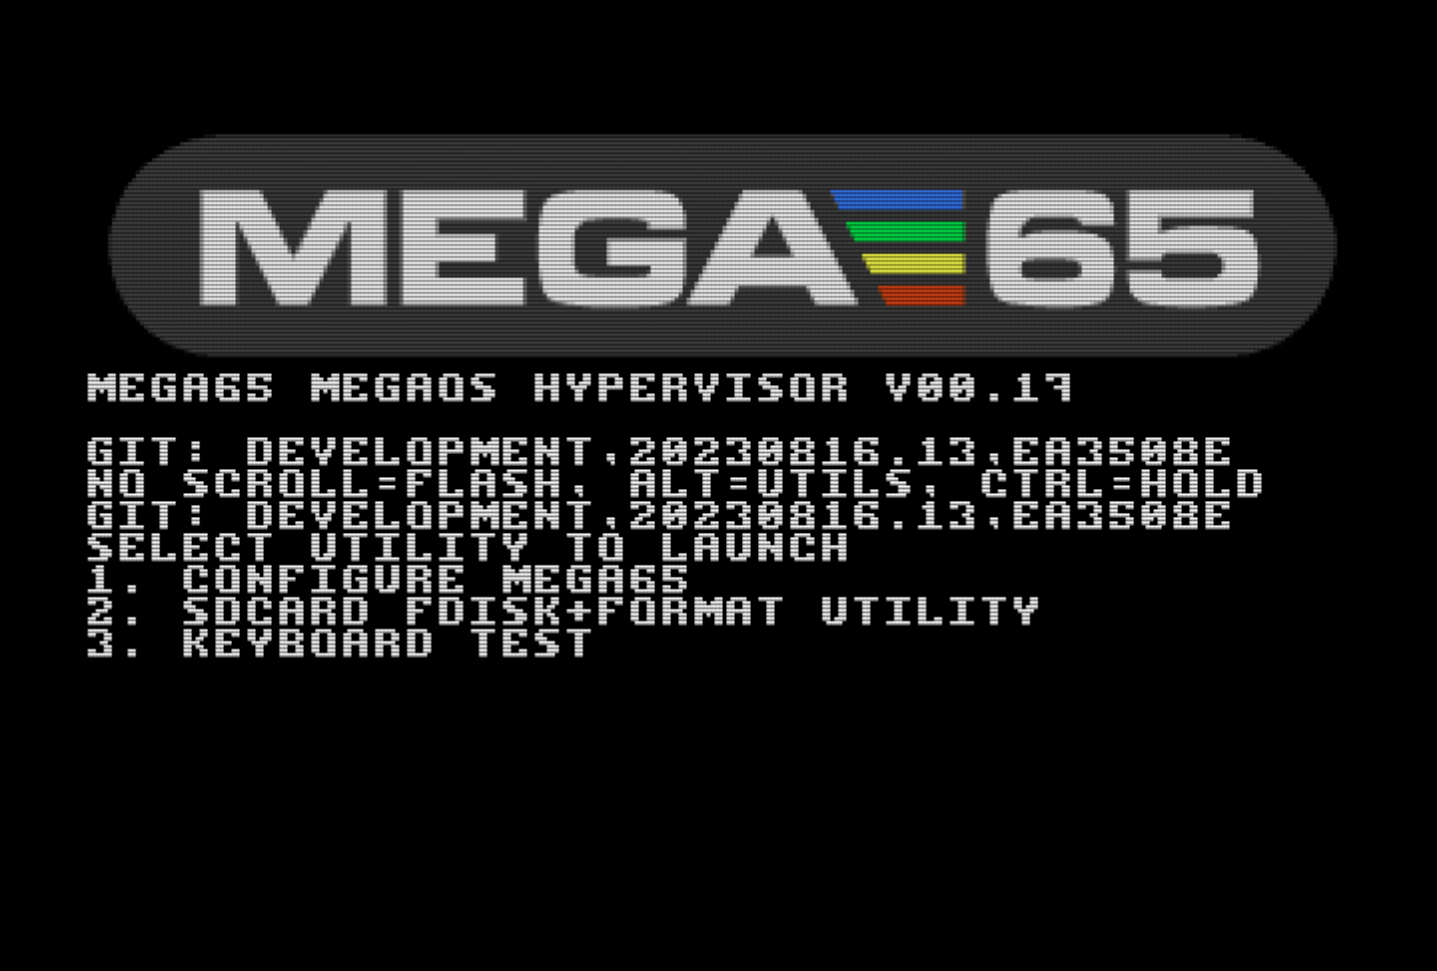
\includegraphics[width=0.7\textwidth]{images/ss-utilmenu.png}
\end{center}

Het SD-kaarthulpprogramma opent en zoekt naar SD-kaarten die in de sleuven zijn geïnstalleerd. Indien u de SD-kaart die u wilt voorbereiden nog niet hebt geplaatst, doe dat nu en druk daarna op \megakey{R} om opnieuw te scannen.

\begin{center}
  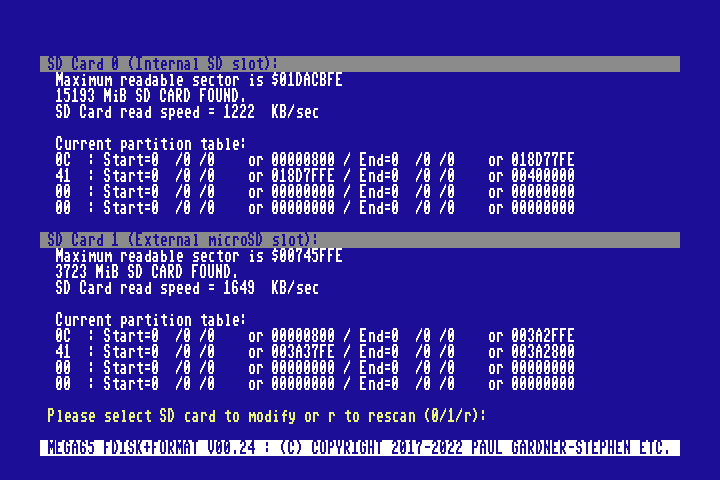
\includegraphics[width=0.7\textwidth]{images/ss-m65fdisk-busselect.png}
\end{center}

Selecteer de kaart die u wilt voorbereiden: \megakey{0} voor de interne SD-kaart, \megakey{1} voor de externe microSD-kaart. Indien er twee kaarten zijn geïnstalleerd, {\em let er goed op dat u de juiste kaartsleuf kiest.}

Het SD-kaarthulpprogramma vraagt bevestiging voordat de SD-kaart wordt gewist. Als allerlaatste voorzorgsmaatregel moet u de tekst {\tt DELETE EVERYTHING} in hoofdletters typen en vervolgens op \specialkey{RETURN} drukken om door te gaan. (Indien u dit proces wilt afbreken, is het veilig om de MEGA65 op dit moment uit te schakelen.)

\begin{center}
  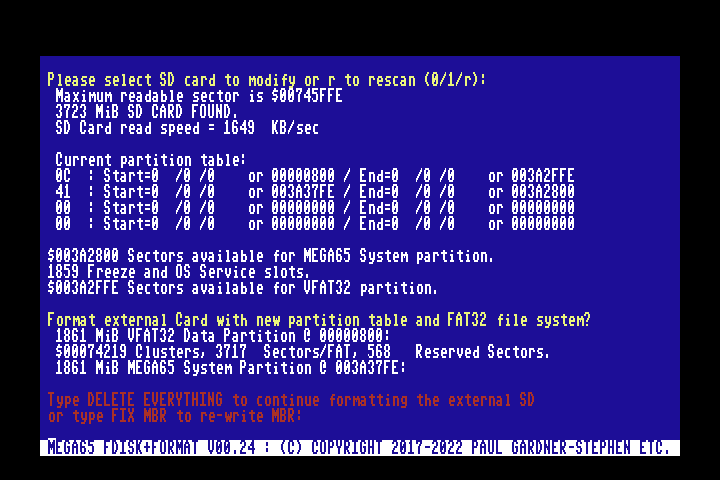
\includegraphics[width=0.7\textwidth]{images/ss-m65fdisk-typesomething.png}
\end{center}

Het hulpprogramma wist de SD-kaart en maakt de partities aan. Wanneer het klaar is, vraagt het of u de systeembestanden wilt installeren. De systeembestanden (met bestandsnamen die eindigen op {\tt .M65} en {\tt .ROM}) zijn in de core ingebed en worden naar de FAT32-partitie gekopieerd voor gebruik. Indien u een bijgewerkte MEGA65-core in slot 1 hebt geïnstalleerd, selecteert u deze; selecteert u anders de in de fabriek geïnstalleerde MEGA65-core in slot 0. (Indien u uw MEGA65 zojuist hebt ontvangen, is slot 0 de enige optie.)

\begin{center}
  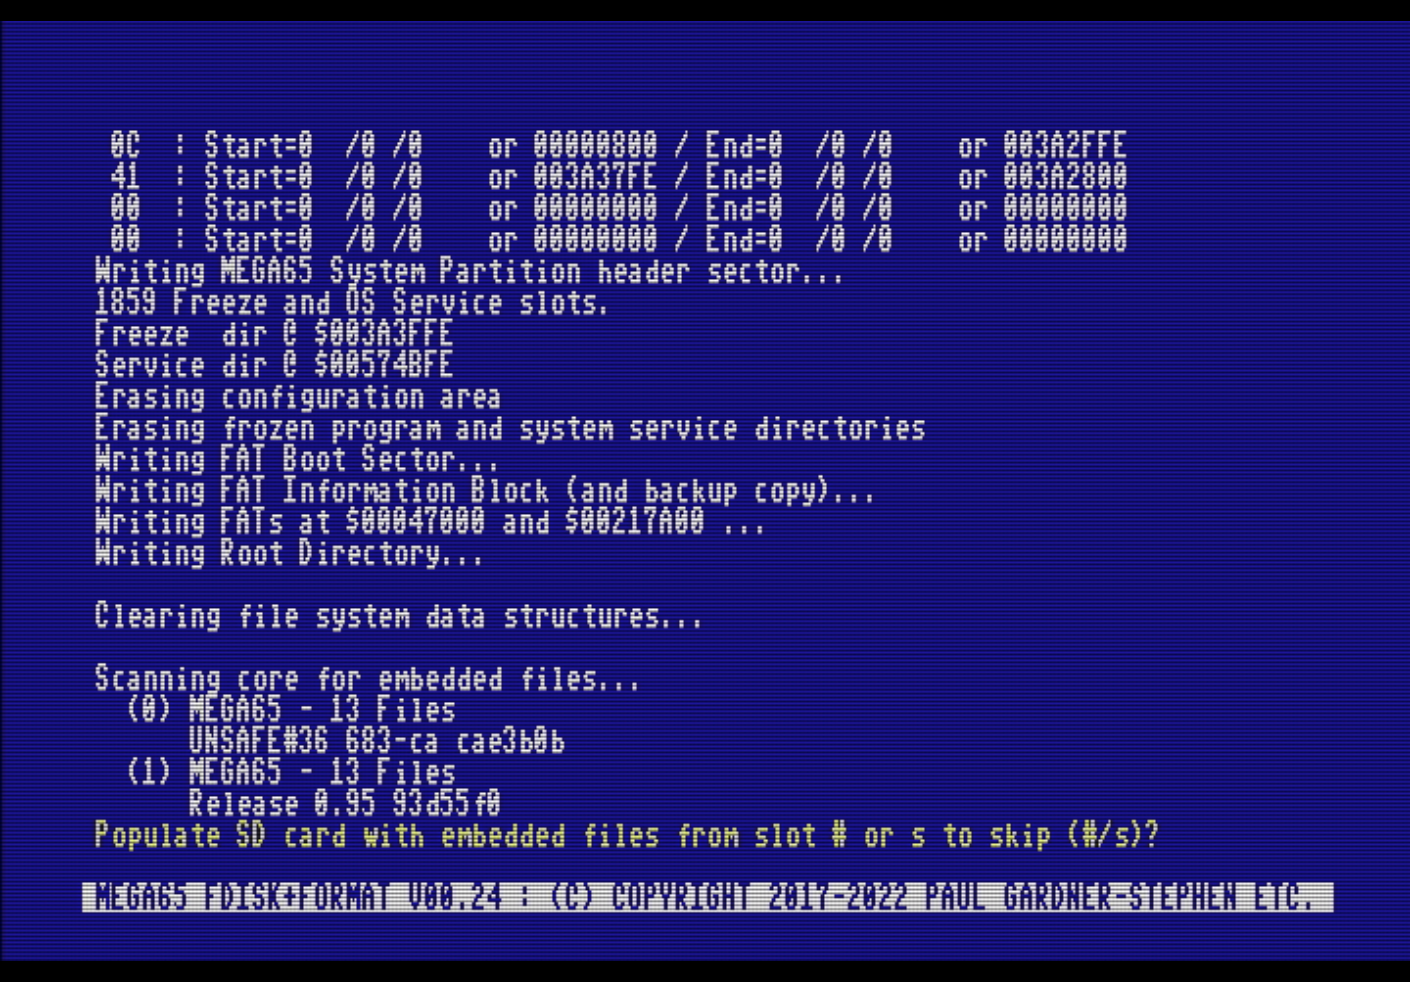
\includegraphics[width=0.7\textwidth]{images/ss-m65fdisk-populate.png}
\end{center}

Start de computer opnieuw op wanneer daarom wordt gevraagd.\footnote{Indien u een core selecteert die {\tt MEGA65.ROM} niet als één van de ingebedde bestanden bevat, vraagt het hulpprogramma u de SD-kaart naar uw PC te verplaatsen om dit bestand erop te kopiëren. Dit gebeurt alleen wanneer u een MEGA65-core gebruikt die afkomstig is van een andere bron dan een officieel MEGA65-releasespakket. Zie voor meer informatie over cores en het verkrijgen van {\tt MEGA65.ROM} hoofdstuk \vref{cha:cores}.}

\subsection{De gebundelde programmatuur verkrijgen}

De systeembestanden die naar de vers geformatteerde SD-kaart worden gekopieerd, omvatten niet de gebundelde programmatuur die bij de oorspronkelijke SD-kaart in de interne kaartsleuf werd meegeleverd. U kunt deze bestanden met uw PC van de oorspronkelijke SD-kaart kopiëren en ze daarna op de nieuwe SD-kaart kopiëren.

De website MEGA65 Filehost\index{Filehost-website} biedt allerlei bestanden aan die u voor uw MEGA65 kunt downloaden. Dit omvat de nieuwste versies van de platformcomponenten, alternatieve cores en honderden spellen, demo's en toepassingen die door de MEGA65-gemeenschap zijn gemaakt. Dit omvat tevens de gebundelde programmatuur van de oorspronkelijke SD-kaart die bij de computer werd meegeleverd.

Indien u de gebundelde softwarebestanden niet meer hebt, kunt u ze verkrijgen via de website MEGA65 Filehost. Bezoek de volgende URL:

\url{https://files.mega65.org/?id=all-intros-public}

\chapter{De MEGA65 upgraden}

\section{Hoe u een MEGA65 kunt upgraden}
\label{cha:cores}

Het MEGA65-platform bestaat uit drie belangrijke onderdelen:

\begin{enumerate}
  \item De {\bf MEGA65-core},\index{Core} een beschrijving van de chipset die op de FPGA draait  \item De {\bf ROM},\index{ROM} code die het besturingssysteem in Commodore-stijl (KERNAL) en BASIC definieert  \item {\bf Systeemsoftware} voor functies zoals het Freezer-menu\index{Freezer-menu}
\end{enumerate}

U kunt deze onderdelen upgraden zodra er nieuwe versies verschijnen. U kunt ook één of meer van deze onderdelen afzonderlijk vervangen. Bij de core en de ROM kunt u zelfs meerdere versies tegelijk geïnstalleerd hebben en daartussen schakelen. In plaats van de nieuwste MEGA65-ROM kunt u bijvoorbeeld overschakelen naar de originele prototype-ROM van de Commodore 65. Of u kunt overschakelen naar een andere core die ervoor zorgt dat uw MEGA65-hardware zich geheel als een andere computer gedraagt, zoals een Commodore 64 of een ZX Spectrum.

De ROM en de systeemsoftware zijn bestanden die op de SD-kaart staan; het upgraden ervan is even eenvoudig als het vervangen van de bestanden. Om de core te upgraden installeert u via een bepaald proces een core-bestand in het core-flashgeheugen van de MEGA65. Dit hoofdstuk beschrijft dit proces.

\subsection{Wat is een core?}
\index{Core!Wat is een core?}

De hardware-architectuur van de MEGA65 is gebaseerd op een veelzijdige chip die een ``Field Programmable Gate Array'' of FPGA wordt genoemd.\index{Field Programmable Gate Array (FPGA)} Dit is een speciaal soort computerchip die geprogrammeerd kan worden om zich als andere chips voor te doen. Het doet dit door een enorme reeks logische poorten zodanig te configureren dat de poorten schakelingen nabootsen. FPGA's zijn geen emulatie, maar een elektronische nabootsing van andere chips. FPGA-code wordt soms aangeduid als {\em firmware,} een term die u wellicht herkent van moderne computers en andere apparaten.

Uw MEGA65 is in de fabriek geprogrammeerd om een chipset na te bootsen die is gebaseerd op de originele Commodore 65 en door het MEGA65-team is ontworpen. U kunt de FPGA van de MEGA65 opnieuw programmeren om te upgraden naar nieuwe versies van de MEGA65-chipset of om de chipset te vervangen door die van een heel andere computer!

Elke mogelijke chipset wordt een {\em core} genoemd. De MEGA65 kan maximaal acht cores opslaan en u kunt tussen deze cores schakelen via een menu dat opent wanneer u de computer inschakelt. U kunt dit menu ook gebruiken om een nieuwe core vanaf een bestand op de SD-kaart te laden, een proces dat {\em flashen} heet.

Leden van de MEGA65-gemeenschap hebben diverse nuttige en leuke alternatieve cores voor de FPGA-hardware gemaakt. \href{https://github.com/MJoergen/C64MEGA65}{{\em C64 voor MEGA65}} van MJoergen en sy2002 bootst de originele Commodore 64-computer met een hoge mate van nauwkeurigheid na en is perfect voor het uitvoeren van Commodore 64-spellen, demo's en toepassingen. Andere cores bootsen de ZX Spectrum, de Game Boy en zelfs de hardware van de originele Galaga-arcademachine na. De FPGA van de MEGA65 is krachtig genoeg om vrijwel alle 8-bit-homecomputers na te bootsen en waarschijnlijk ook enkele 16-bit-computers en spelcomputers, zoals de Commodore Amiga. Het hardware-ontwerp van de MEGA65, de indeling van het moederbord, de FPGA-core en overige informatie zijn allemaal gratis beschikbaar onder diverse openbronlicenties, zodat iedereen vrij is andere cores voor de MEGA65-hardware te maken.

\section{De versies van de onderdelen bepalen}
\label{sec:versions}

Alle onderdelen van het MEGA65-platform hebben een versieaanduiding. De MEGA65 kan de versieaanduidingen van al zijn onderdelen weergeven met het MEGA65-informatiehulpprogramma.\index{MEGA65-informatiehulpprogramma}

Om het MEGA65-informatiehulpprogramma te openen:

\begin{enumerate}
  \item Schakel de MEGA65 in en laat hem opstarten tot BASIC.  \item Open de Freezer:\index{Freezer-menu} houd \widekey{RESTORE} één seconde ingedrukt en laat hem daarna los.  \item Druk op \specialkey{HELP}. Het MEGA65-informatiehulpprogramma opent.
\end{enumerate}

\begin{center}
  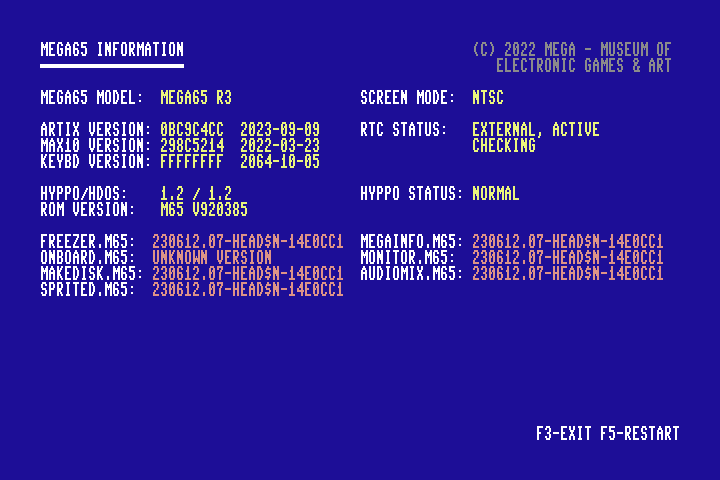
\includegraphics[width=0.7\linewidth]{images/megainfo.png}
\end{center}

Noteer deze versieaanduidingen:
\nopagebreak
\begin{center}
\setlength{\tabcolsep}{1mm}
\begin{tabularx}{\textwidth}{|X|p{7cm}|}
  \hline
  {\bf Label en voorbeeld} & {\bf Beschrijving} \\
  \hline
  MEGA65-model\newline {\tt MEGA65 R6} & De revisie van de hardware. U moet dit weten wanneer u nieuwe core-bestanden downloadt. \\
  \hline
  Artix-versie\index{Core!Versies}\newline {\tt 8AD00DD7 2024-01-22} & De MEGA65-core die op dit moment draait. Dit is een reeks van acht letters en cijfers en tevens een builddatum. \\
  \hline
  ROM-versie\index{ROM!Versie}\newline {\tt M65 V920393} & De ROM die op dit moment draait. Voor MEGA65-ROM's is dit een oplopend nummer, waarbij grotere nummers nieuwere versies aanduiden. \\
  \hline
  Systeembestanden (.M65)\newline {\tt 240122.21-R0.3.0-8B6C767} & Elk bestand van de systeemsoftware heeft een eigen versieaanduiding. Gewoonlijk hoeft u deze niet te kennen: u upgradet deze gelijktijdig met elke core. De aanduiding lijkt op de core-versie, doch komt niet altijd overeen met de core die op dat moment draait. \\
  \hline
\end{tabularx}
\end{center}

Druk op \megakey{F3} om terug te keren naar de Freezer en druk daarna nogmaals op \megakey{F3} om terug te keren naar BASIC.

Elke core heeft een afzonderlijke versie voor elke hardware-revisie. Vanaf het jaar 2024 gebruiken de productiemodellen van de MEGA65 twee verschillende moederbordrevisies, welke bekend staan als ``R3'' (meer specifiek ``R3A'') en ``R6''.\footnote{Het MEGA65-``DevKit''-model dat in het jaar 2020 werd verkocht, is van revisie ``R3''. Het is tevens mogelijk de MEGA65-core op bepaalde FPGA-ontwikkelborden te laten draaien, met voor elk bord een afzonderlijke versie van het core-bestand.}\index{Hardware-revisies}

De MEGA65-core is voor alle hardware-revisies beschikbaar. Indien u een alternatieve core installeert die niet beschikbaar is voor uw hardware-revisie, neem dan contact op met de auteur van de core.

\section{De nieuwste bestanden verkrijgen}

U kunt de nieuwste MEGA65-core, ROM en systeemsoftware downloaden van de website van de MEGA65-Filehost.\index{Filehost-website} Vanwege distributiebeperkingen voor de ROM-code van de Commodore 65 kunnen sommige bestanden alleen worden gedownload met een Filehost-account dat op naam van een MEGA65-eigenaar staat. Alle eigenaren van de MEGA65 hebben een licentie voor alle versies van deze ROM-code.\footnote{Er bestaat een procedure voor niet-eigenaren om de nieuwste MEGA65-ROM te verkrijgen, bijvoorbeeld om te gebruiken met de \href{https://github.lgb.hu/xemu/}{Xemu MEGA65 emulator}. Deze procedure houdt in dat u \href{https://www.c64forever.com/}{C64 Forever Free Express Edition} van Cloanto downloadt, het originele prototype-ROM-bestand van de Commodore 65 extraheert en vervolgens een hulpmiddel gebruikt om een patch toe te passen die u van Filehost kunt downloaden. Het volledige proces wordt beschreven in het volgende artikel: \url{https://mega65.org/rom-faq}}

Bezoek de volgende URL in uw webbrowser:

\url{https://files.mega65.org}

\begin{center}
  \fbox{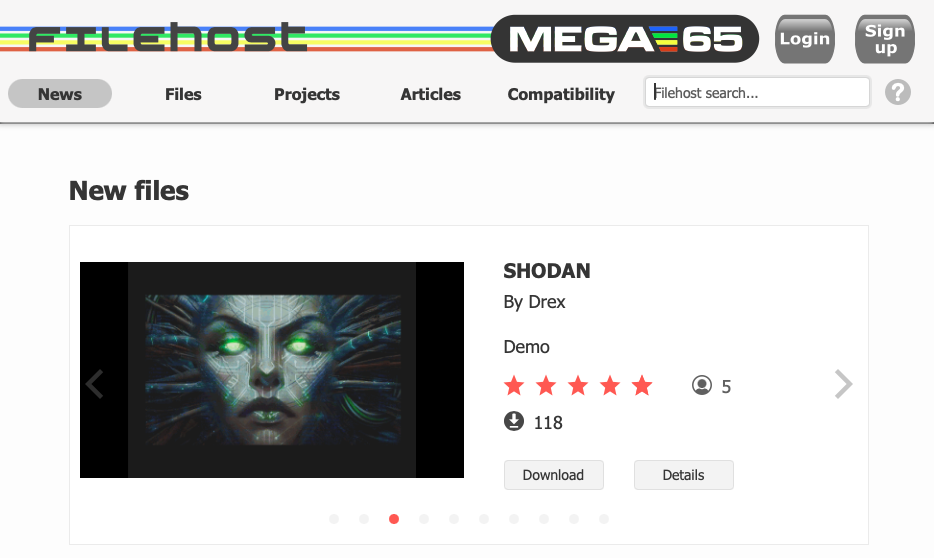
\includegraphics[width=0.7\linewidth]{images/filehost_notsignedin.png}}
\end{center}

Om een Filehost-account met uw eigenaarcode te registreren:

\begin{enumerate}
  \item Bezoek \href{https://files.mega65.org}{de Filehost-website}. Klik op ``Sign Up''. Volg de aanwijzingen om een account aan te maken.  \item Zoek uw eigenaarcode op.\index{Eigenaarscode} Dit is een code die op een papiertje staat afgedrukt; het papiertje was bij uw MEGA65 inbegrepen (mogelijk is het in deze handleiding gestoken). De code ziet er ongeveer als volgt uit: {\tt 123-ABC-456}  \item Klik in de rechterbovenhoek van het Filehost-scherm op het gebruikerspictogram. Selecteer in het pop-upmenu ``Redeem Code''. Voer uw eigenaarcode in zoals gevraagd.
\end{enumerate}

\begin{center}
  \fbox{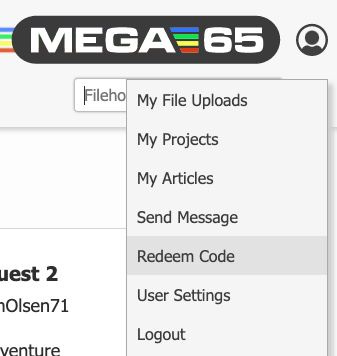
\includegraphics[width=0.4\linewidth]{images/filehost_redeemmenu.png}}
\end{center}

Om het nieuwste releasepakket te downloaden:

\begin{enumerate}
  \item Klik op het tabblad ``Files'' van de Filehost-website.  \item Typ in het zoekvak aan de linkerkant: ``core release''. De lijst wordt bijgewerkt en toont vervolgens alleen bestanden met deze woorden in de titel.  \item Zoek de vermelding genaamd ``MEGA65 Core Release Package (mega65r6) with ROM'', waarbij ``mega65r6'' overeenkomt met uw hardware-revisie. (Om uw hardware-revisie te bevestigen opent u het Freezer-menu en drukt u daarna op \specialkey{HELP}.)  \item Klik op de vermelding. Bevestig dat dit releasepakket voor uw hardware-revisie is en klik daarna op ``Download'' om het bestand te downloaden.
\end{enumerate}

\underline{OPMERKING}: Er bestaat een vermelding van het releasepakket zonder de ROM. Deze vermelding is voor iedereen zichtbaar. Om er zeker van te zijn dat u een compatibele set bestanden gebruikt, kiest u het pakket waarop ``with ROM'' staat. Indien u geen vermelding ziet waarop ``with ROM'' staat, controleer dan of u bent aangemeld en of u een geldige eigenaarcode heeft ingewisseld.

\begin{center}
  \fbox{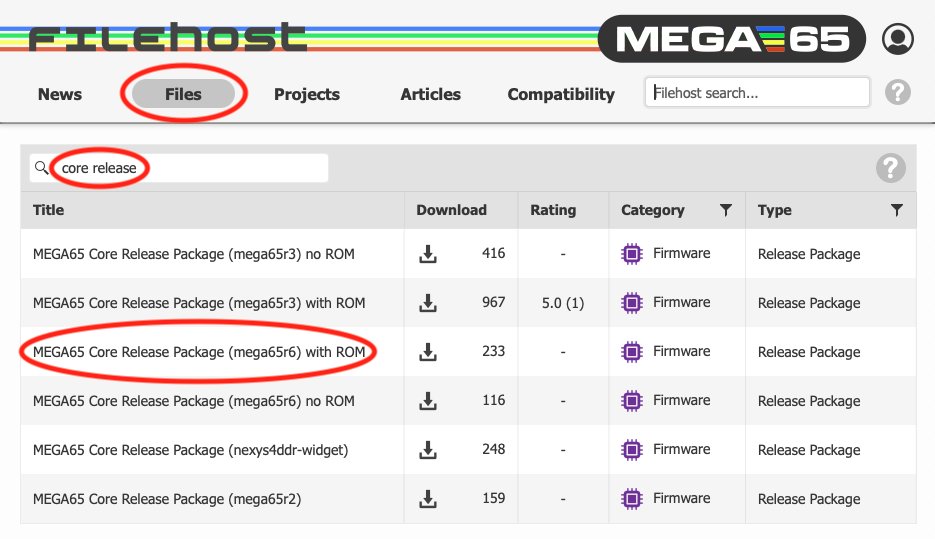
\includegraphics[width=0.7\linewidth]{images/filehost_release.png}}
\end{center}

Pak het gedownloade {\tt .7z}-archief uit. U zou een bestand moeten zien waarvan de naam eindigt op {\tt .cor} en een map {\tt sdcard-files} die een bestand bevat met de naam {\tt MEGA65.ROM}.

\section{Het corekeuzemenu}
\index{Core!Corekeuzemenu}

De MEGA65 bepaalt welke core bij het opstarten in de FPGA wordt geladen. U kunt dit proces onderbreken om te kiezen welke core wordt geladen.\footnote{Strikt genomen start de MEGA65 de core in slot 0 op om het corekeuzemenu te laten draaien. Nadat u een keuze hebt gemaakt of de computer een standaardcore kiest, laadt de computer de gekozen core in de FPGA en vervolgt hij het opstartproces.}

Om het corekeuzemenu te openen schakelt u de computer uit, houdt u de toets \specialkey{NO\\SCROLL} ingedrukt en schakelt u de computer weer in. Het corekeuzemenu verschijnt, met de acht coreslots, genummerd van 0 tot en met 7.

\begin{center}
  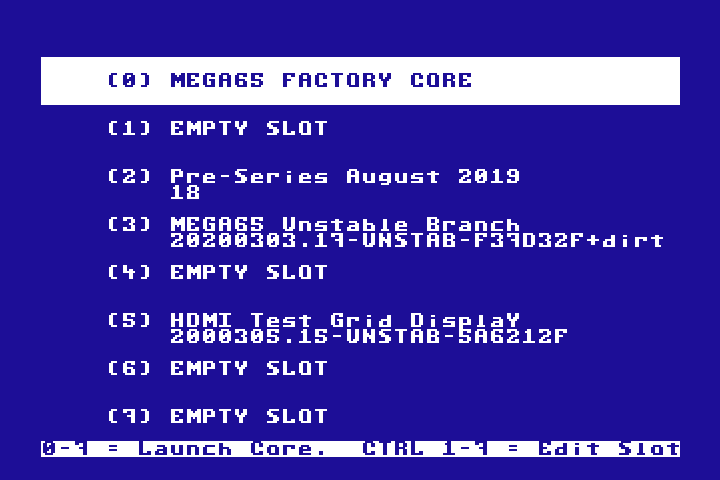
\includegraphics[width=0.7\linewidth]{images/ss-flashmenu.png}
\end{center}

U kunt met de cursortoetsen en \specialkey{RETURN} een core kiezen om op te starten, of u kunt eenvoudigweg de cijfertoets indrukken die overeenkomt met het slot. Het opstartproces wordt voortgezet met de nieuwe core. De MEGA65 blijft de nieuwe core gebruiken totdat u de computer uitschakelt. (Het indrukken van de resetknop wijzigt niet welke core wordt gebruikt.)

Wanneer u de computer inschakelt zonder het corekeuzemenu te openen, zoekt de MEGA65 naar een standaardcore. De computer controleert eerst of een core als standaardcore is gemarkeerd (een instelling die u kunt wijzigen). Indien geen enkele core zo is gemarkeerd, controleert de computer daarna of er een core in slot 1 staat.\footnote{Indien DIP-schakelaar \#4 in de stand ``on'' staat, controleert de MEGA65 slot 2 in plaats van slot 1. De DIP-schakelaars bevinden zich in de behuizing, op het moederbord.} Indien het slot leeg is, gebruikt de computer slot 0.

Uw computer is in de fabriek uitgerust met de MEGA65-core in slot 0. Wij raden u aan de in de fabriek geïnstalleerde core niet te upgraden, tenzij het MEGA65-team u dat adviseert. Installeer nieuwe versies van de MEGA65-core in plaats daarvan in slot 1.

\section{De core, ROM en systeembestanden upgraden}
\index{Core!Upgraden}\index{ROM!Upgraden}

Vanuit het corekeuzemenu kunt u een core upgraden of een nieuwe core installeren. Tijdens dit proces leest de computer het bestand {\tt .cor} van de SD-kaart.

Om de MEGA65-core, ROM en systeembestanden te upgraden:

\begin{enumerate}
  \item Verwijder de SD-kaart (of microSD-kaart) uit de MEGA65 en sluit deze met een SD-kaartlezer aan op uw PC.\footnote{In plaats van de SD-kaart naar uw PC over te brengen kunt u de bestanden ook via een Ethernet-verbinding overzetten. Zie hoofdstuk \vref{cha:transferring-files}.}  \item Kopieer het {\tt .cor}-bestand dat u uit het {\tt .7z}-archief hebt gehaald naar de SD-kaart.  \item Open op uw PC de map {\tt sdcard-files} uit het {\tt .7z}-archief en kopieer deze bestanden daarna naar de SD-kaart, waarbij u de bestaande bestanden vervangt. Plaats ze in de hoofdmap van het bestandssysteem van de SD-kaart, niet in een submap.  \item Werp de SD-kaart uit via het besturingssysteem van uw PC en plaats deze daarna terug in de MEGA65.  \item Open het corekeuzemenu: schakel de MEGA65 uit en houd daarna \specialkey{NO\\SCROLL} ingedrukt terwijl u de computer weer inschakelt.  \item Houd \specialkey{CTRL} ingedrukt en druk daarna op het cijfer van het slot dat u wilt upgraden. De sloteditor opent.  \item Druk op \megakey{F3} om een core-bestand te laden. De bestandsselectie opent. Gebruik de cursortoetsen om het {\tt .cor}-bestand te selecteren en druk daarna op \specialkey{RETURN}.  \item Druk op \megakey{F8} om het coreslot te flashen. Laat het flashen volledig verlopen. Dit duurt enkele minuten.  \item Wanneer het flashen is voltooid, drukt u op een willekeurige toets om terug te keren naar het corekeuzemenu.
\end{enumerate}

De sloteditor ziet er als volgt uit:

\begin{center}
  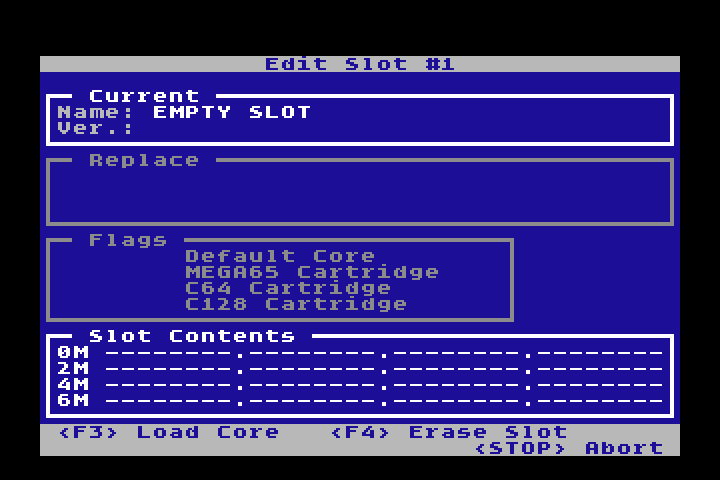
\includegraphics[width=0.7\linewidth]{images/ss-flashmenu-sloteditor.png}
\end{center}

Wanneer u een core-bestand laadt, vraagt de computer u het {\tt .cor}-bestand te selecteren op een scherm dat op dit voorbeeld lijkt:

\begin{center}
  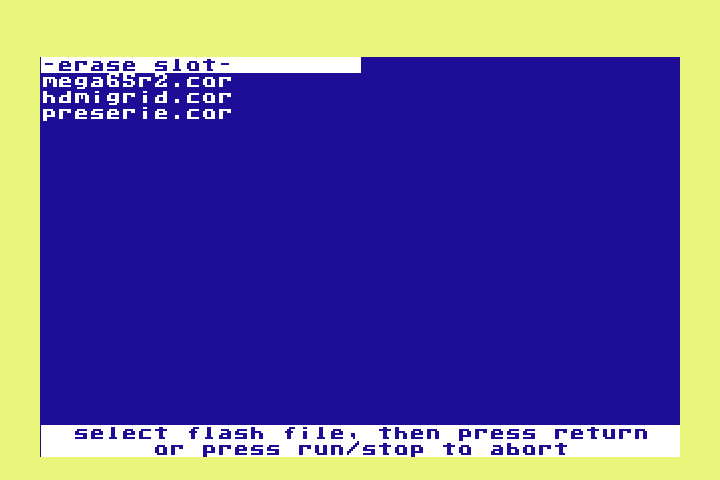
\includegraphics[width=0.7\linewidth]{images/ss-flashmenu-selectcore.png}
\end{center}

Nadat u de core hebt geselecteerd, toont de sloteditor welke wijziging deze in het slot wil aanbrengen. Wanneer u het flashen start, toont het beeldscherm de voortgang.

\underline{OPMERKING}: Schakel uw computer {\em niet} uit en onderbreek de stroomtoevoer niet voordat deze stap is voltooid.

\begin{center}
  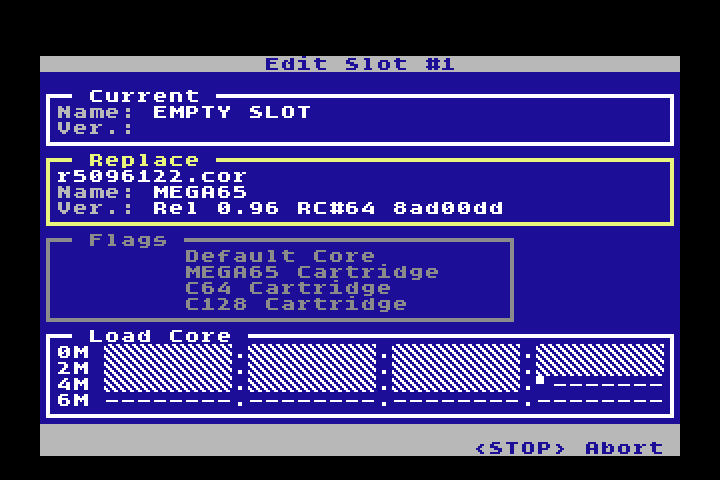
\includegraphics[width=0.7\linewidth]{images/ss-flashmenu-loading.png}
\end{center}

Wanneer de melding "Core was successfully flashed" wordt weergegeven, is het proces voltooid.

\begin{center}
  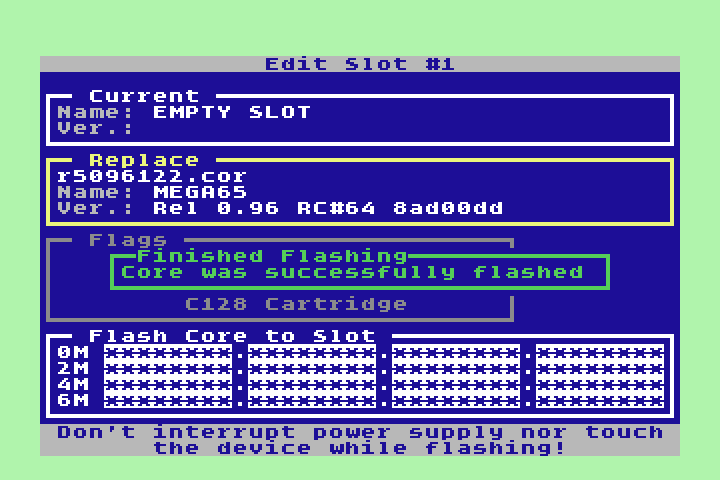
\includegraphics[width=0.7\linewidth]{images/ss-flashmenu-complete.png}
\end{center}

Het is nu veilig om uw computer uit te schakelen. Druk op een willekeurige toets om terug te keren naar het corekeuzemenu, of schakel de computer uit en daarna weer in om de standaardcore te starten.


\section{Alternatieve cores en ROM's installeren}

Het installeren van een alternatieve core, zoals de C64-core,\index{Core!C64-core} verloopt volgens dezelfde stappen voor het flashen van de core naar een slot.

Het is raadzaam de slots 2 tot en met 7 voor alternatieve cores te gebruiken en slot 1 voor de nieuwste MEGA65-core te reserveren. Er staat u uiteraard niets in de weg om een alternatieve core in slot 1 te installeren, zodat de MEGA65 zich bij het inschakelen als een ander type computer gedraagt. De MEGA65-core kunt u altijd kiezen via het corekeuzemenu.

U kunt meer dan één versie van de MEGA65-ROM op de SD-kaart bewaren. Wanneer u de MEGA65-core opstart, kunt u één van deze ROM's selecteren door tijdens het opstarten een cijfertoets ingedrukt te houden.

Om alternatieve ROM's te installeren kopieert u ze naar de hoofdmap van de SD-kaart, met een bestandsnaam zoals {\tt MEGA65x.ROM}, waarbij {\tt x} een getal tussen 0 en 8 is. Om de alternatieve ROM op te starten houdt u de bijbehorende cijfertoets ingedrukt terwijl de MEGA65-core start. Indien u geen cijfer ingedrukt houdt, start de computer standaard {\tt MEGA65.ROM} op.

Er zijn verschillende redenen waarom u alternatieve ROM's op uw SD-kaart zou willen bewaren:

\begin{itemize}
  \item U helpt een nieuwe bètaversie van de ROM te testen en u wilt de bètaversie niet tot uw standaard-ROM maken.
  \item U wilt de originele prototype-ROM van de Commodore 65 proberen. De MEGA65-core behoudt de achterwaartse compatibiliteit met de C65-ROM waaraan Commodore werkte voordat het bedrijf het project annuleerde. Deze ROM is gebrekkig en onvolledig, maar vormt nog steeds een interessant historisch artefact.
  \item U wilt een alternatieve ROM proberen die door de MEGA65-gemeenschap is ontwikkeld. Eén van deze ROM's is de MEGA65 OpenROM, een project om een volledig nieuwe ROM te maken die onder een open-sourcelicentie wordt uitgebracht, zonder enig oorspronkelijk Commodore-materiaal.
\end{itemize}

Bij uw MEGA65-SD-kaart werden diverse alternatieve ROM's meegeleverd, die in de fabriek zijn geïnstalleerd. Probeer uw computer opnieuw op te starten terwijl u een cijfertoets ingedrukt houdt en kijk wat er gebeurt!

\section{Core-vlaggen instellen}

Er zijn verschillende opties (``vlaggen'') die u voor een core in de core-editor kunt kiezen.

Om vlaggen voor een core te wijzigen bewerkt u het coreslot. Druk op de cijfertoets die overeenkomt met de vlag om de waarde ervan om te schakelen. Sla de vlaggen in het slot op door het resultaat te flashen: druk op \megakey{F8}. U kunt de vlaggen vóór het flashen van nieuwe coregegevens instellen, of u kunt alleen de nieuwe vlaginstellingen flashen zonder de coregegevens te vervangen.

Om een core in te stellen als de standaardcore, welke wordt gebruikt wanneer de MEGA65 wordt ingeschakeld zonder \specialkey{NO\\SCROLL} ingedrukt te houden, stelt u de vlag "Default core" in. Indien geen enkele core als standaardcore is ingesteld, wordt slot 1 als standaard gebruikt (of slot 2 indien DIP-schakelaar \#4 in de stand ``on'' staat).

De vlaggen "cartridge" bepalen welke core wordt geselecteerd wanneer er een cartridge in de expansiepoort aanwezig is. Zo kunt u op basis van het type cartridge een andere standaardcore kiezen. U kunt bijvoorbeeld de MEGA65-core instellen om MEGA65-cartridges af te handelen en een andere core om C64-cartridges af te handelen. Standaard handelt de MEGA65-core C64-cartridges af met behulp van de "GO64"-modus. Wellicht geeft u er de voorkeur aan dit te wijzigen en de C64-core te gebruiken die u afzonderlijk installeert.

\begin{center}
  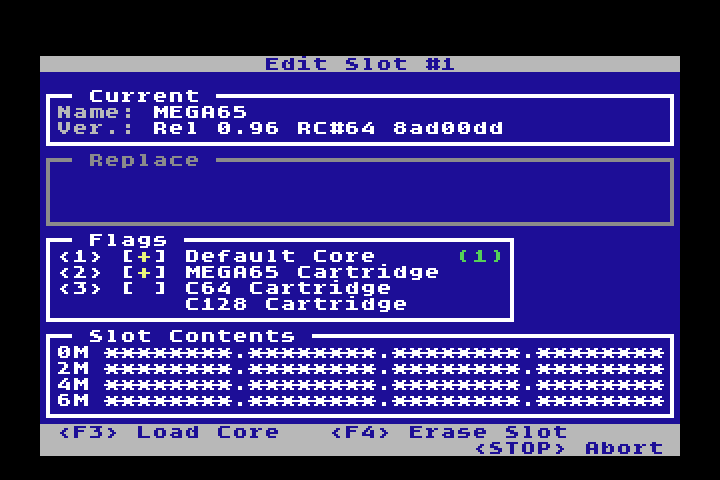
\includegraphics[width=0.7\linewidth]{images/ss-flashmenu-flags.png}
\end{center}

\section{Een coreslot wissen}

Het flashen vervangt wat er in een coreslot staat door de nieuwe core. Indien er al een core in het slot is geïnstalleerd, overschrijft het flashen de bestaande core.

Indien u een core wilt verwijderen en het slot leeg wilt laten, bewerkt u het slot en drukt u op \megakey{F4} om de vervanging in te stellen op "Erase slot". Druk daarna op \megakey{F8} om het slot met lege gegevens te flashen.

\section{De fabriekscore in slot 0 upgraden}
\index{Core!Fabriekscore in slot 0 upgraden}

Het is mogelijk de in de fabriek geïnstalleerde MEGA65-core in slot 0 te upgraden. Dit hoeft u alleen in zeldzame gevallen te doen, bijvoorbeeld indien een nieuwere versie van de MEGA65-core wijzigingen of foutcorrecties voor het opstartproces bevat. Het is raadzaam slot 0 niet te upgraden, tenzij de aankondiging van de uitgave daartoe aanleiding geeft. De meeste upgrades van de MEGA65-core zijn in slot 1 volledig functioneel, zonder dat u slot 0 hoeft te upgraden.

Het is belangrijk dat ten minste één coreslot een werkende MEGA65-core bevat. Indien er tijdens het flashen iets misgaat, kan dit leiden tot een niet-werkende core in dat slot. Om ongelukken te helpen voorkomen verschilt de procedure voor het flashen van slot 0 enigszins van die van de andere slots en kan alleen een officiële MEGA65-core naar slot 0 worden geflasht.

{\em Lees deze aanwijzingen zorgvuldig door voordat u met de procedure begint.} Om de core in slot 0 te upgraden:

\begin{enumerate}
  \item Installeer de nieuwste MEGA65-core in slot 1 met behulp van de hierboven beschreven procedure. De core moet zich in het standaardslot ongelijk aan nul bevinden om van eventuele problemen bij het upgraden van slot 0 te kunnen herstellen.  \item Start coreslot 1 op om te bevestigen dat het werkt.  \item Keer terug naar het corekeuzemenu: schakel de MEGA65 uit en houd daarna \specialkey{NO\\SCROLL} ingedrukt terwijl u de computer weer inschakelt.  \item Houd \megasymbolkey ingedrukt en druk op de komma-toets om de editor voor slot 0 te openen.  \item Lees het informatiescherm en typ daarna het woord {\tt CONFIRM} in hoofdletters en druk op \specialkey{RETURN}.  \item Herhaal de rest van de flashprocedure om het core-bestand te selecteren en het slot te flashen.
\end{enumerate}

\underline{OPMERKING}: Indien u een MEGA65 van revisie R3A heeft en slot 0 nog niet eerder heeft geüpgraded, starten \megasymbolkey en de komma-toets de procedure niet: u heeft een oudere core in slot 0 die deze voorziening niet heeft. U kunt dit omzeilen door het corekeuzemenu opnieuw te starten met slot 1. Bereid u vanuit het corekeuzemenu voor om \specialkey{NO\\SCROLL} ingedrukt te houden, druk op \megakey{1} om de core op te starten en druk daarna onmiddellijk op \specialkey{NO\\SCROLL} en houd deze ingedrukt. Het corekeuzemenu wordt daarna opnieuw geopend met behulp van slot 1. Druk op \megasymbolkey en de komma-toets om de upgrade van slot 0 te voltooien.

Indien er tijdens het flashen van slot 0 iets misgaat, start uw MEGA65 mogelijk niet correct op. Schakel uw MEGA65 vóór al het andere in en wacht ongeveer een minuut. Na enige tijd zou de computer moeten merken dat er geen geldige core in slot 0 staat en vervolgens de core in slot 1 starten. U kunt tijdens dit proces \specialkey{NO\\SCROLL} ingedrukt houden om het corekeuzemenu van slot 1 te openen en het flashen opnieuw te starten.

Indien de MEGA65 na enkele minuten nog geen enkele core kan opstarten, is de computer mogelijk vastgelopen. U kunt de computer wellicht herstellen met behulp van een apparaat dat een ``JTAG-interface'' heet en uw PC met het moederbord van de MEGA65 verbindt. Hiermee kunt u een bitstream rechtstreeks in de FPGA injecteren. Het onderdeel is goedkoop, doch niet altijd verkrijgbaar. Neem voor hulp contact op met het MEGA65-team via de Discord (\url{https://mega65.org/chat}).

Aan coreslot 0 kunnen geen vlaggen worden toegewezen, zoals een vlag om als standaardcore te dienen of om aan cartridgetypen te worden gekoppeld. Slot 0 wordt voor deze doeleinden gebruikt indien er geen andere core is geïnstalleerd. Het is raadzaam de nieuwste MEGA65-core in slot 1 te bewaren, naast het flashen van slot 0.


\section{Het opstartproces van de core begrijpen}
\nopagebreak
Deze sectie vat samen hoe de MEGA65 kiest met welke core hij bij het inschakelen opstart. Het proces wordt weergegeven in de volgende afbeelding:
\nopagebreak
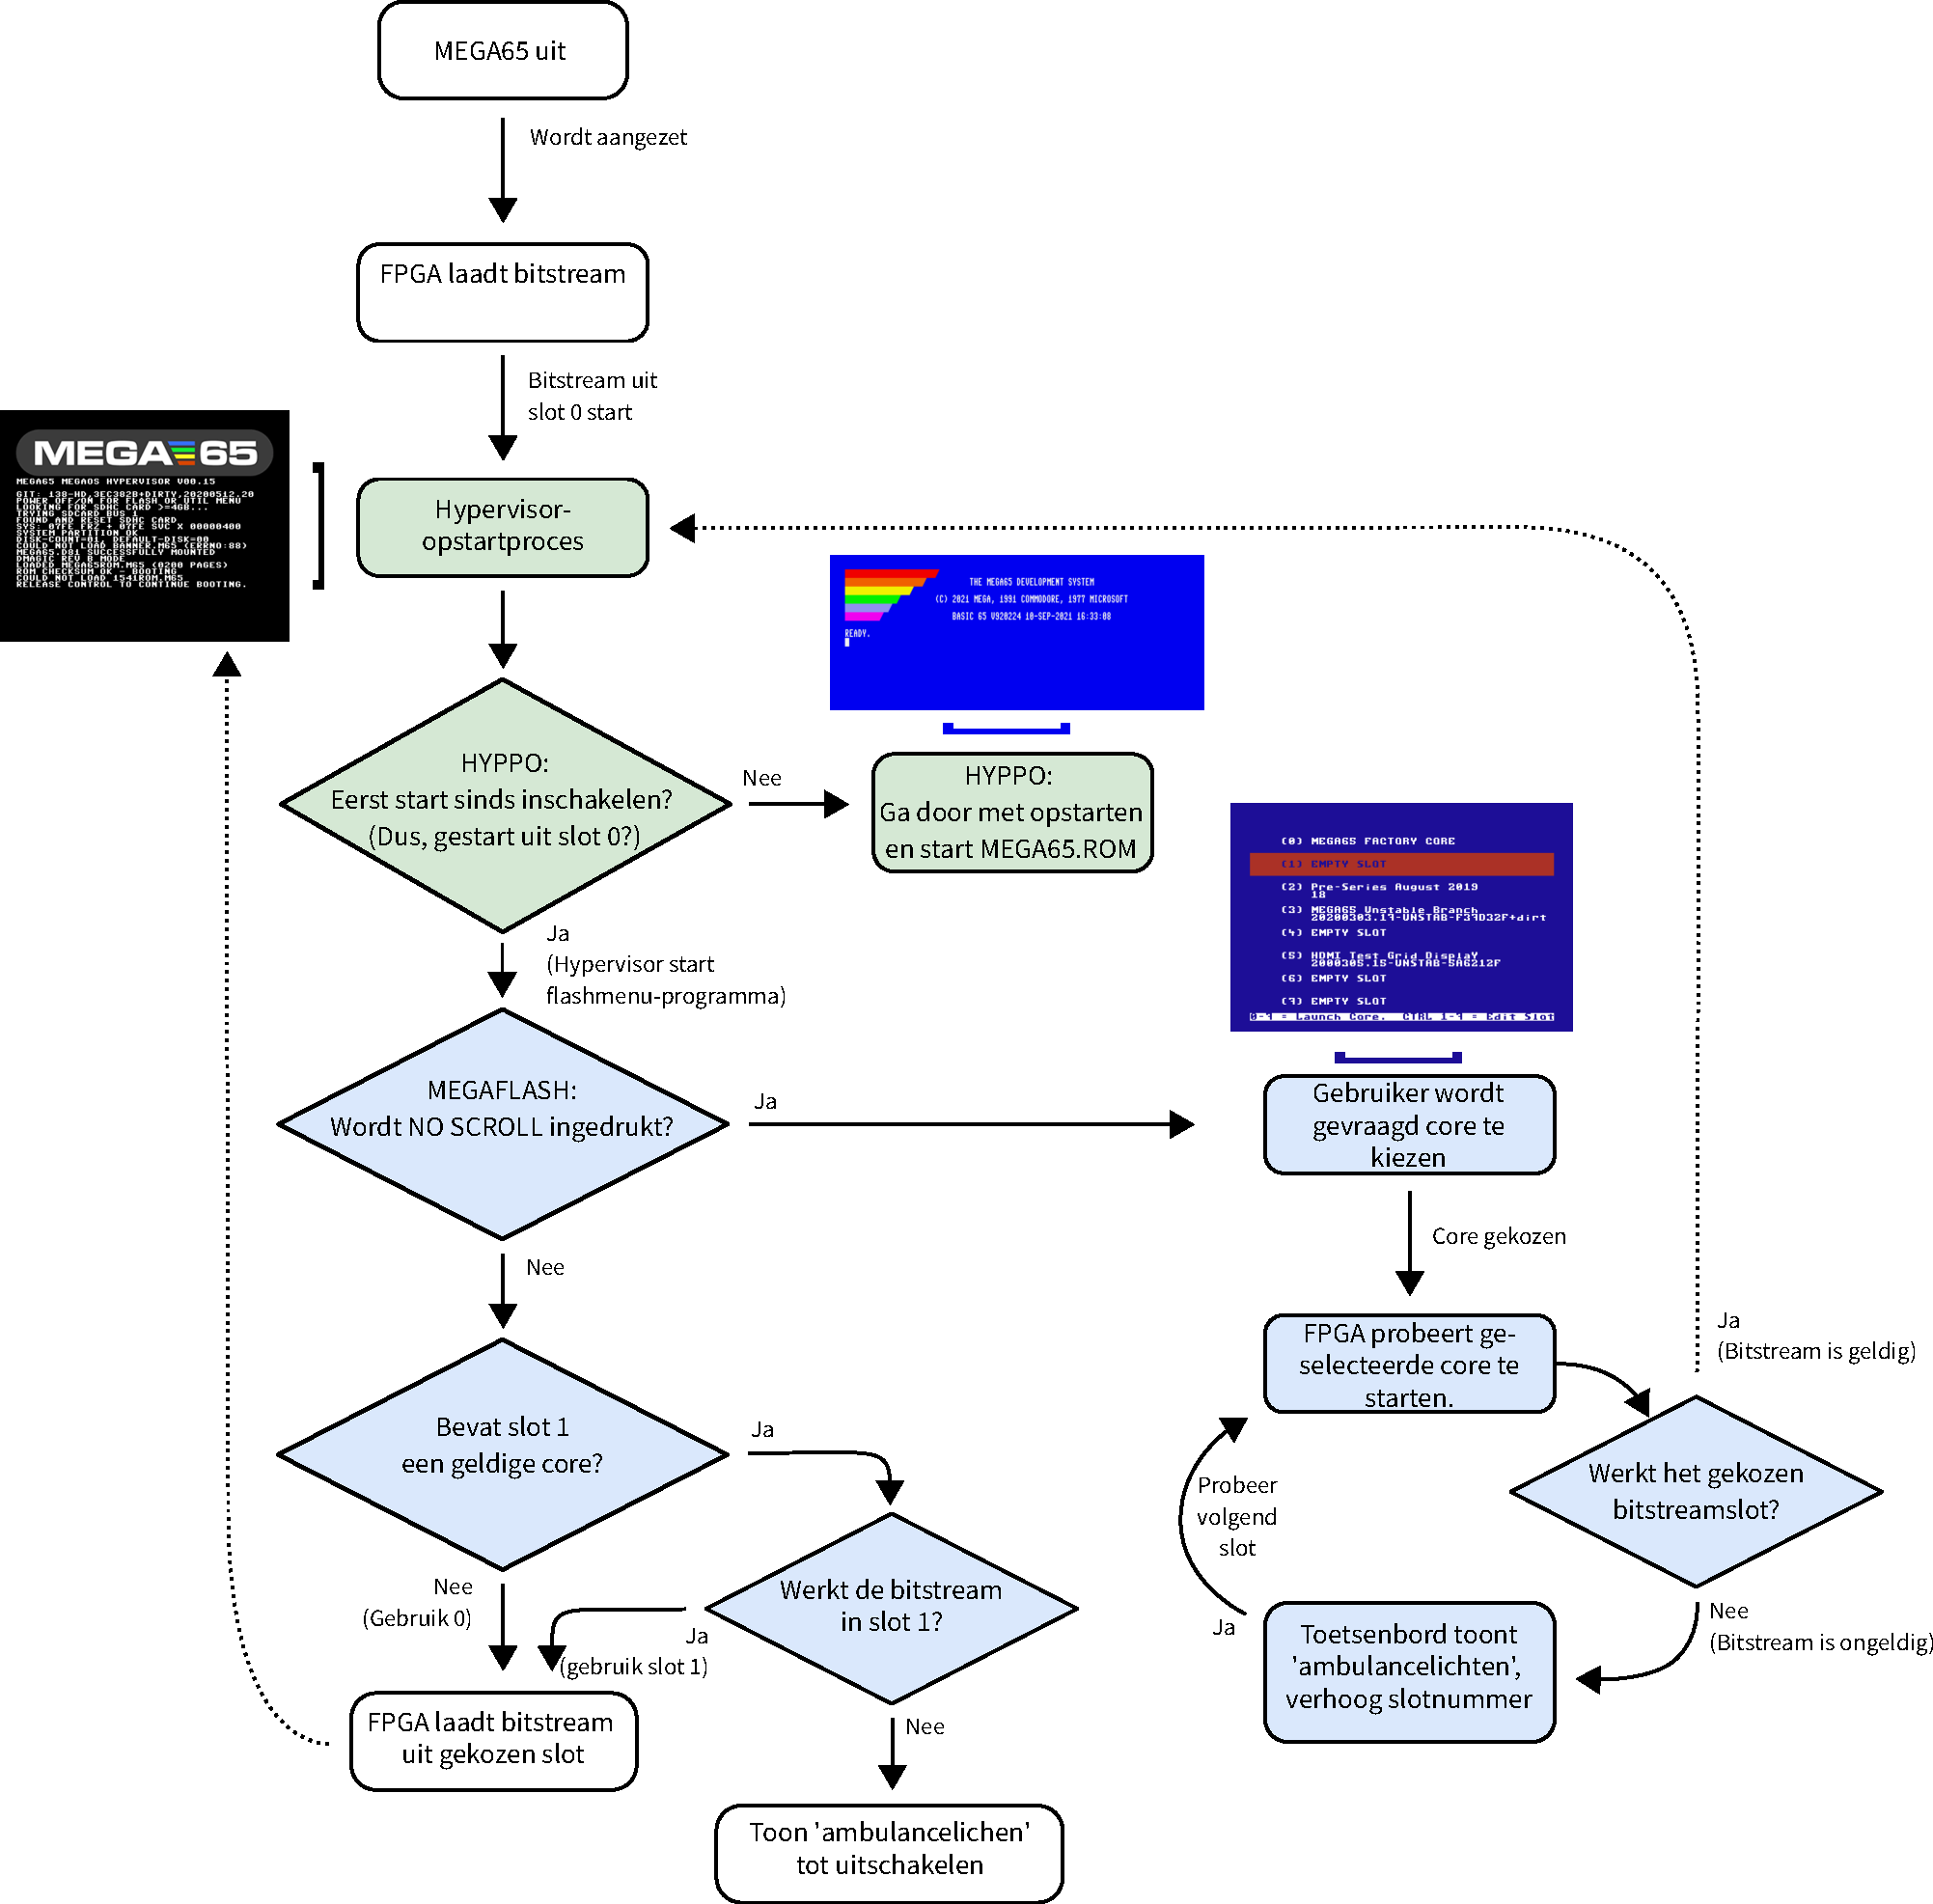
\includegraphics[width=\linewidth]{dutch/images/illustrations/flashmenu-flowchart.pdf}

Het opstartproces wordt beheerd door twee voorzieningen:
\begin{itemize}
  \item De Hypervisor (ook bekend als HYPPO), welke op een niveau boven de KERNAL werkt. Eén van zijn taken is het beheren van delen van het opstartproces. Raadpleeg voor meer details over de Hypervisor
\ifdefined\printmanual
{\bf Het grote Mega65-boek}.
\else
 \bookvref{sec:hypervisor-mode}.
\fi
    In het diagram zijn de activiteiten die de Hypervisor uitvoert groen gemarkeerd.  \item Het corekeuzemenuprogramma (ook bekend als ``MegaFlash''), welke een lijst met beschikbare coreslots biedt om uit te kiezen. In het diagram zijn de activiteiten die MegaFlash uitvoert blauw gemarkeerd.
\end{itemize}

Wanneer de MEGA65 wordt ingeschakeld, doet de computer het volgende:
\begin{itemize}
\item De MEGA65 laadt de bitstream in slot 0 van het flashgeheugen. Indien dat de MEGA65-fabriekscore is, start de HYPPO-hypervisor van de MEGA65.\item Indien het de eerste opstart na het inschakelen is (wat betekent dat u vanuit slot 0 werkt), start HYPPO het Flash-menu-programma (ook wel MegaFlash genoemd) -- maar houd er rekening mee dat het Flash-menu in deze modus mogelijk niets op het scherm toont om aan te geven dat het draait!\item Het Flash-menu controleert vervolgens of \specialkey{NO\\SCROLL} ingedrukt wordt gehouden.\item Indien dat het geval is, toont het Flash-menu zijn scherm, zodat u een core kunt selecteren of opnieuw flashen.\item Indien \specialkey{NO\\SCROLL} {\em niet} wordt ingedrukt gehouden, controleert het Flash-menu of Flash-slot 1 een geldige core bevat.\item Indien dat zo is, probeert het Flash-menu die core te laden.\item Indien dit lukt, herconfigureert het systeem zichzelf voor die core, waarna het gedrag van het systeem overeenkomt met die core.\item Indien dit mislukt, schakelt het toetsenbord over naar de ``ambulancemodus'', waarbij blauwe lampjes knipperen om aan te geven dat er eerste hulp nodig is. Merk op dat de resetknop in de ambulancemodus geen effect heeft: u moet de MEGA65 uitschakelen en weer inschakelen.
\end{itemize}

Indien u in het corekeuzemenu een andere core hebt geselecteerd, verloopt het proces op vergelijkbare wijze, met dit verschil dat de ambulancelampjes slechts gedurende een beperkte tijd branden: de FPGA zoekt namelijk automatisch door het flashgeheugen totdat hij een geldige core vindt. Indien hij het einde van het flashgeheugen bereikt, start hij de MEGA65-fabriekscore opnieuw vanuit slot 0.

\chapter{Werken met schijven en schijfimages}

\section{Schijfstations}
\label{cha:using-disks}
\index{Schijfstations}

De MEGA65 beschikt over een ingebouwd 3.5"-diskettestation en ondersteunt externe schijfstations in Commodore-stijl via de seriële IEC-poort aan de achterzijde van de computer. De IEC-poort ondersteunt ook andere externe IEC-opslagapparaten, zoals de SD2IEC.\index{SD2IEC-apparaat} Sommige IEC-opslagapparaten kunt u in een keten aansluiten en tegelijkertijd gebruiken.

De MEGA65 bevat ook een ``virtueel'' schijfstation dat D81- of D64-schijfimagebestanden\index{D81-schijfimage}\index{D64-schijfimage} op de SD-kaart kan aankoppelen. De meeste MEGA65-programmatuur die u van het internet downloadt, heeft de vorm van een D81-schijfimage. Programma's voor de Commodore 64 worden vaak verspreid in de vorm van een D64-schijfimage. U kunt rechtstreeks vanaf de MEGA65 een nieuw D81-schijfimage aanmaken en uw BASIC-programma's op de SD-kaart opslaan, zonder dat u extra hardware nodig hebt. U kunt ook bestanden kopiëren tussen fysieke floppy-schijven en schijfimages.

Het Intro Disk-menu\index{Intro Disk} dat u zag toen u de computer voor het eerst inschakelde, is een programma op een D81-schijfimage: een bestand met de naam {\tt MEGA65.D81} op de SD-kaart. De MEGA65 is in eerste instantie geconfigureerd om dit schijfimage automatisch op te starten. U kunt dit wijzigen in het Configuratiehulpprogramma.\index{Configuratie!Hulpprogramma} (Zie ook hoofdstuk \vref{cha:configuringyourmega}.)

U kunt schijfstations en virtuele schijfimages vanuit het Freezer-menu beheren.\index{Freezer-menu} Sommige van deze handelingen kunt u uitvoeren met BASIC-commando's zoals {\bf MOUNT}.\index{BASIC 65-commando's!MOUNT}

\subsection{Unitnummers en drivenummers}
\index{Schijfstations!Unitnummers en drivenummers}
\index{Aansluitingen!IEC}

Elk schijfstation (fysiek of virtueel) wordt benaderd via een {\it unit}nummer.\index{Unitnummer (IEC-apparaten)} Bij de vintage Commodore-computers verwijst het unitnummer naar een IEC-apparaat dat op de computer is aangesloten. Commodore reserveerde de unitnummers in het bereik 0 -- 31 voor apparaten met uiteenlopende doeleinden, waarvan 8 -- 11 voor schijfstations. Hebt u ooit een Commodore 64 gebruikt en \screentext{LOAD "*",8,1} ingetypt, dan verwijst de ``8'' naar het schijfstation dat als unit 8 is aangesloten. De schijfcommando's van BASIC 65 gebruiken standaard unit 8 en aanvaarden een {\bf U}-parameter om dit te wijzigen, bijvoorbeeld: \screentext{DLOAD "MYPROGRAM",U9}\index{BASIC 65-voorbeelden!DLOAD}\index{BASIC 65-voorbeelden!LOAD}

Bij de MEGA65 kunt u een unitnummer toewijzen aan het virtuele schijfstation met een gekoppeld schijfimage, of aan het ingebouwde 3.5"-diskettestation. U moet een schijfimage of het ingebouwde 3.5"-diskettestation aan een unitnummer koppelen voordat het gebruikt kan worden. Elk bericht dat naar een unitnummer wordt gestuurd dat aan een virtuele schijf of het ingebouwde diskettestation is toegewezen, wordt door de MEGA65 afgehandeld. Alle overige berichten worden naar de seriële IEC-poort gestuurd.

Schijfcommando's aanvaarden ook een optionele parameter om een {\it drive}nummer op te geven.\index{Drivenummer (IEC-apparaten)} Deze is alleen nodig bij het aansluiten van een vintage dubbel diskettestation via de IEC-poort, zoals de Commodore 4040, 8050 of 8250. Elk schijfstation kent drivenummer 0 toe aan het eerste station. Stations met twee schijven kennen drivenummer 1 toe aan het tweede station. Dubbele schijfstations zijn gewoonlijk uitgerust met een IEEE-488-interface en hebben een IEEE-488-naar-IEC-omzetter nodig om op de MEGA65 gebruikt te kunnen worden. De schijfcommando's van BASIC 65 gebruiken standaard drive 0 en aanvaarden een {\bf D}-parameter om dit te wijzigen.


\section{Werken met virtuele schijfimages}
\index{Schijfstations!Virtuele schijfimages}

De MEGA65 biedt twee ``beheerde stations'' die de via de IEC-poort aangesloten stations aanvullen. Aan het eerste beheerde station kunt u een D81- of D64-schijfimagebestand op de SD-kaart toewijzen, of u kunt het toewijzen aan het ingebouwde 3.5"-diskettestation. Aan het tweede beheerde station kunt u eveneens een D81- of D64-schijfimagebestand toewijzen, zodat er maximaal twee virtuele schijven tegelijkertijd gekoppeld kunnen worden.\footnote{Commodore was oorspronkelijk van plan een nieuw extern 3.5"-diskettestation uit te brengen, het ``1565''-station, dat bij de Commodore 65 zou horen en op een speciale niet-IEC-poort zou worden aangesloten. Het MEGA65-project heeft de ambitie om zo'n station ooit te produceren; indien dat gebeurt, zou dit station aan het tweede beheerde station worden toegewezen.}

Het eerste beheerde station kan worden ingesteld op unit 8 of 10 en het tweede beheerde station op unit 9 of 11.

\subsection{Waar u schijfimagebestanden kunt verkrijgen}

De website MEGA65 Filehost\index{Filehost-website} herbergt een bibliotheek met MEGA65-programmatuur die door de gemeenschap is gemaakt. U kunt door de programmatuur bladeren of erin zoeken, een titel downloaden en het schijfimage vervolgens met uw pc of met het Ethernet-bestandsoverdrachtshulpprogramma naar de SD-kaart kopiëren.

\url{https://files.mega65.org/}

\subsection{Schijfimages aankoppelen met de Freezer}

Open het Freezer-menu:\index{Freezer-menu} houd \widekey{RESTORE} één seconde ingedrukt en laat de toets vervolgens los. Let op de huidige toestand van aangekoppelde stations rechtsonder op het scherm.

\begin{center}
  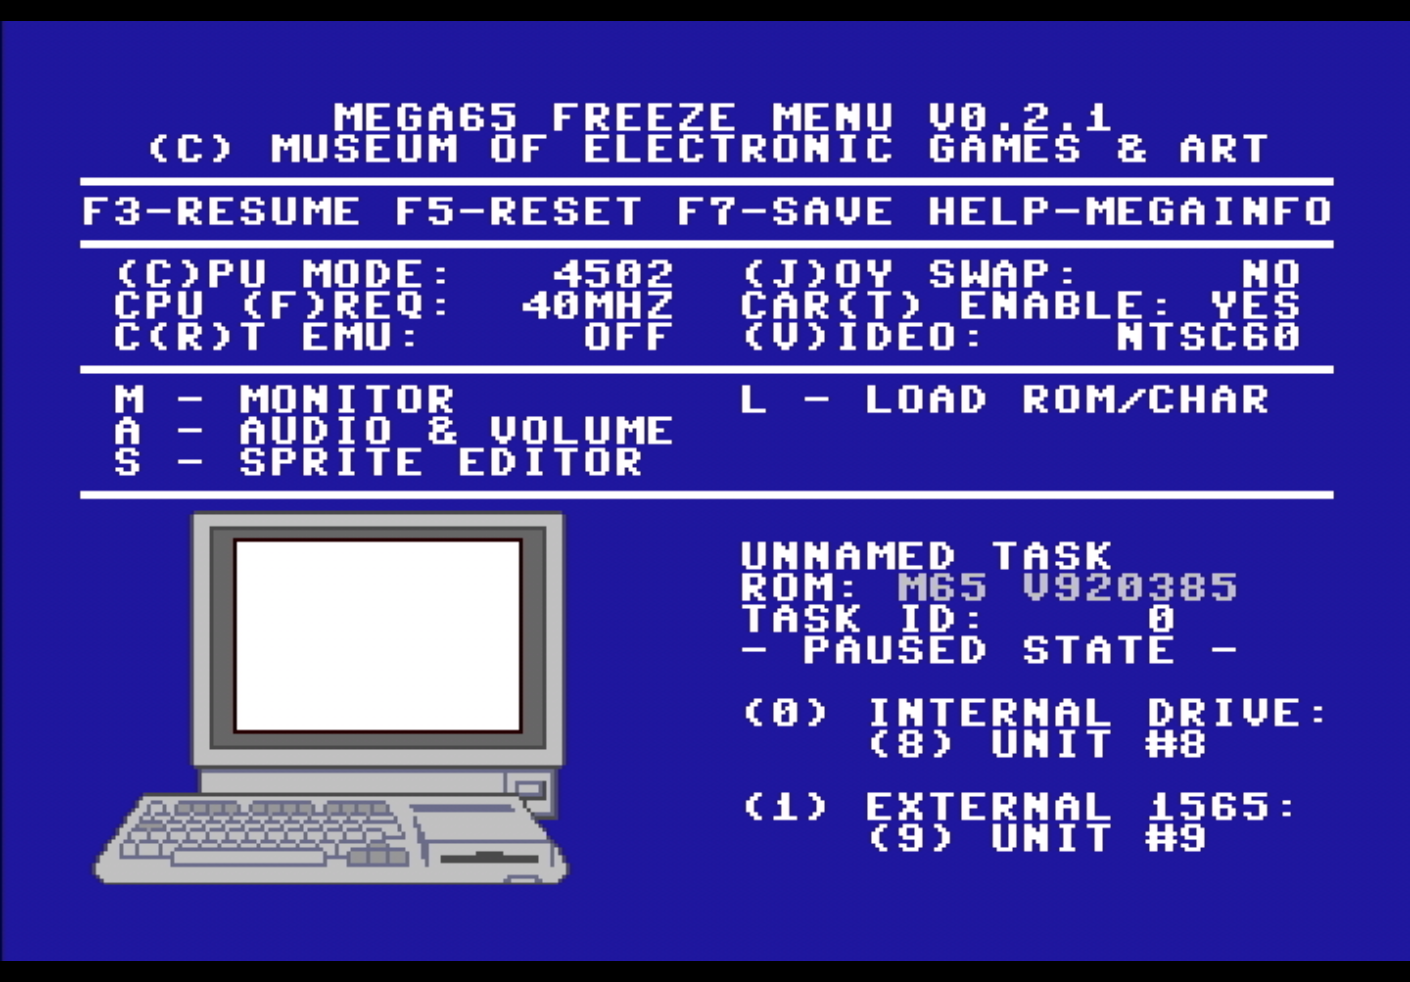
\includegraphics[width=0.7\linewidth]{images/freezer.png}
\end{center}

Om een schijfimage aan unit 8 of 10 te koppelen, selecteert u het eerste beheerde station door op \megakey{0} te drukken. Om een schijfimage aan unit 9 of 11 te koppelen, selecteert u het tweede beheerde station door op \megakey{1} te drukken. Dit opent de bestandsbrowser van de SD-kaart.

\begin{center}
  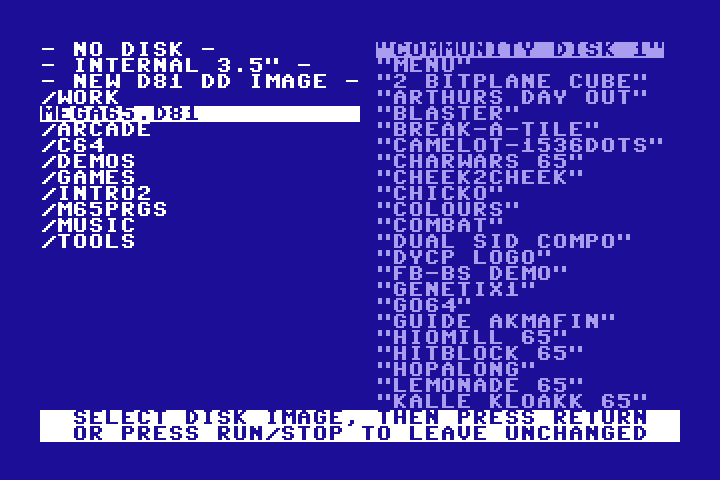
\includegraphics[width=0.7\linewidth]{images/d81-file-browser.png}
\end{center}

Gebruik de cursortoetsen om een schijfimage te selecteren en druk vervolgens op \widekey{RETURN}. Het Freezer-scherm toont dat het geselecteerde schijfimage nu aan het beheerde station is gekoppeld.

Druk vanaf het hoofdscherm van de Freezer op \megakey{8} of \megakey{9} om te wisselen tussen de unitnummers van respectievelijk het eerste en het tweede beheerde station.

\subsection{Schijfimages aankoppelen vanuit BASIC}

Met het BASIC-commando {\bf MOUNT}\index{BASIC 65-commando's!MOUNT} kunt u een schijfimage vanaf de SD-kaart aankoppelen zonder de Freezer te hoeven openen. U kunt dit commando bij de \screentext{READY}-prompt invoeren of het als onderdeel van een programma gebruiken.

Om een schijfimage aan unit 8 te koppelen, voert u {\bf MOUNT} in met de volledige bestandsnaam tussen dubbele aanhalingstekens, inclusief het achtervoegsel {\tt .D81} of {\tt .D64}:

\begin{screencode}
MOUNT "MEGA65.D81"
\end{screencode}

Om een schijfimage aan unit 9 te koppelen, geeft u het {\bf U}-argument op:

\begin{screencode}
MOUNT "MEGA65.D81",U9
\end{screencode}

\subsection{Een nieuw schijfimage aanmaken}
\index{Schijfstations!Virtuele schijfimages}

U kunt vanuit de Freezer van de MEGA65 een nieuw leeg D81-schijfimage aanmaken.\index{Freezer-menu}

\begin{enumerate}
\item Open de Freezer.\item Druk op \megakey{0} om het eerste beheerde station te selecteren.\item Selecteer boven in de bestandenlijst: \screentext{- NEW D81 DD IMAGE -}\item Voer, wanneer u daarom gevraagd wordt, een naam voor de schijf in. (Laat het achtervoegsel {\tt .D81} weg; dit wordt automatisch toegevoegd.)
\end{enumerate}

Het nieuwe schijfimage wordt op de SD-kaart aangemaakt en aan het eerste beheerde station gekoppeld. Het is geformatteerd en gereed voor gebruik.

\subsection{SD-kaartbestanden beheren in submappen}

Wanneer u enige tijd op Filehost games en toepassingen hebt gedownload, zult u uiteindelijk een grote verzameling schijfimages op uw SD-kaart hebben. Mogelijk wilt u deze bestanden in submappen ordenen. U kunt deze mappen aanmaken terwijl de SD-kaart op uw pc is aangesloten, of met het Ethernet-bestandsoverdrachtshulpprogramma.

De Freezer ondersteunt submappen in de bestandsbrowser. Elke submapnaam begint met een schuine streep (\screentext{/}). Selecteer een map om de bestanden ervan weer te geven. Om terug te keren naar de vorige map, selecteert u: \screentext{/..}

De MEGA65 houdt een ``huidige werkmap'' bij die als basismap dient voor BASIC-commando's zoals {\bf MOUNT}. Om de huidige werkmap vanuit BASIC te wijzigen, gebruikt u het {\bf CHDIR}-commando\index{BASIC 65-commando's!CHDIR} met het {\bf U12}-argument:\index{BASIC 65-voorbeelden!CHDIR}\index{BASIC 65-voorbeelden!MOUNT}

\begin{screencode}
CHDIR "DEMOS",U12

MOUNT "XANADU.D81"
\end{screencode}

\underline{OPMERKING}: De ondersteuning voor submappen op de SD-kaart is nog in ontwikkeling. Indien een schijfimage in een submap is gekoppeld, wordt het ontkoppeld door elke handeling die de huidige werkmap wijzigt. Sommige voorzieningen die bestanden gebruiken, ondersteunen mogelijk geen bestanden in submappen. Het is momenteel niet mogelijk om vanuit de Freezer een nieuw schijfimage in een submap aan te maken. Wij hopen dit in een toekomstige update te verbeteren.


\section{Het ingebouwde 3.5"-diskette\-station gebruiken}

De MEGA65 beschikt over een ingebouwd 3.5"-diskettestation, vergelijkbaar met wat voor de Commodore 65 bedoeld was. U kunt fysieke floppy-schijven gebruiken om uw programma's en gegevens op te slaan. Sommige MEGA65-programmatuur kan op diskette worden aangeschaft.

Het ingebouwde 3.5"-diskettestation moet gekoppeld worden voordat het gebruikt kan worden. Het kan aan unit 8 of unit 10 worden gekoppeld, in het eerste beheerde station.

\subsection{Het ingebouwde 3.5"-station aankoppelen met de Freezer}

Open het Freezer-menu:\index{Freezer-menu} houd \widekey{RESTORE} één seconde ingedrukt en laat de toets vervolgens los. Let op de huidige instellingen voor het aankoppelen van stations rechtsonder op het scherm.

Druk op \megakey{0} en gebruik vervolgens de pijltjestoets omlaag om \screentext{- INTERNAL 3.5" -} te selecteren. Druk op \widekey{RETURN} om de selectie te bevestigen. Het Freezer-menu toont dat het interne station aan het eerste beheerde schijfstation is gekoppeld.

Het \screentext{UNIT \#} voor het eerste station kan 8 of 10 zijn. Druk op \megakey{8} om tussen deze opties te wisselen. De schijfcommando's van BASIC 65 gebruiken standaard unit 8, dus het is gebruikelijk unit 8 te gebruiken tenzij u tegelijkertijd met meerdere schijven werkt.

Het ingebouwde 3.5"-diskettestation kan alleen in het eerste beheerde station worden gekoppeld, met unitnummers 8 of 10. Het kan niet in het tweede beheerde station worden gekoppeld (unitnummers 9 of 11).

\subsection{Het ingebouwde 3.5"-station aankoppelen vanuit BASIC}

U kunt het ingebouwde 3.5"-diskettestation met het BASIC-commando {\bf MOUNT} aan unit 8 koppelen. Dit commando werkt zowel vanaf de \screentext{READY}-prompt als vanuit een programma. Om het interne station aan unit 8 te koppelen, voert u het commando zonder argumenten in:\index{BASIC 65-voorbeelden!MOUNT}

\begin{screencode}
MOUNT
\end{screencode}

Het {\bf MOUNT}-commando kan het interne station alleen aan unit 8 koppelen. Vanuit het Freezer-menu kunt u het alleen aan unit 10 koppelen.

\subsection{DD- en HD-schijven}
\index{Schijfstations!Double-densityschijven (DD)}
\index{Schijfstations!High-densityschijven (HD)}

De schijfcontroller van de MEGA65 verwacht een diskette met Double Density (DD) in het ingebouwde 3.5"-diskettestation.\footnote{Het is mogelijk dat HD-schijven met volledige capaciteit in een toekomstige firmware-update worden ondersteund. De hardware van het station kan HD-schijven lezen.} Floppy-schijven worden niet meer geproduceerd en de DD-variant is tegenwoordig moeilijk te vinden.

U kunt een diskette met High Density (HD) in het station gebruiken, mits u één belangrijke wijziging aanbrengt: u moet beide zijden van het gat in de linkerbovenhoek (van voren gezien) van de schijf bedekken met een klein stukje plakband. Hierdoor laat u het station geloven dat de schijf DD is en schakelt het over naar een modus die compatibel is met de schijfcontroller van de MEGA65. Een DD-schijf heeft op deze plaats geen gat.

\begin{center}
  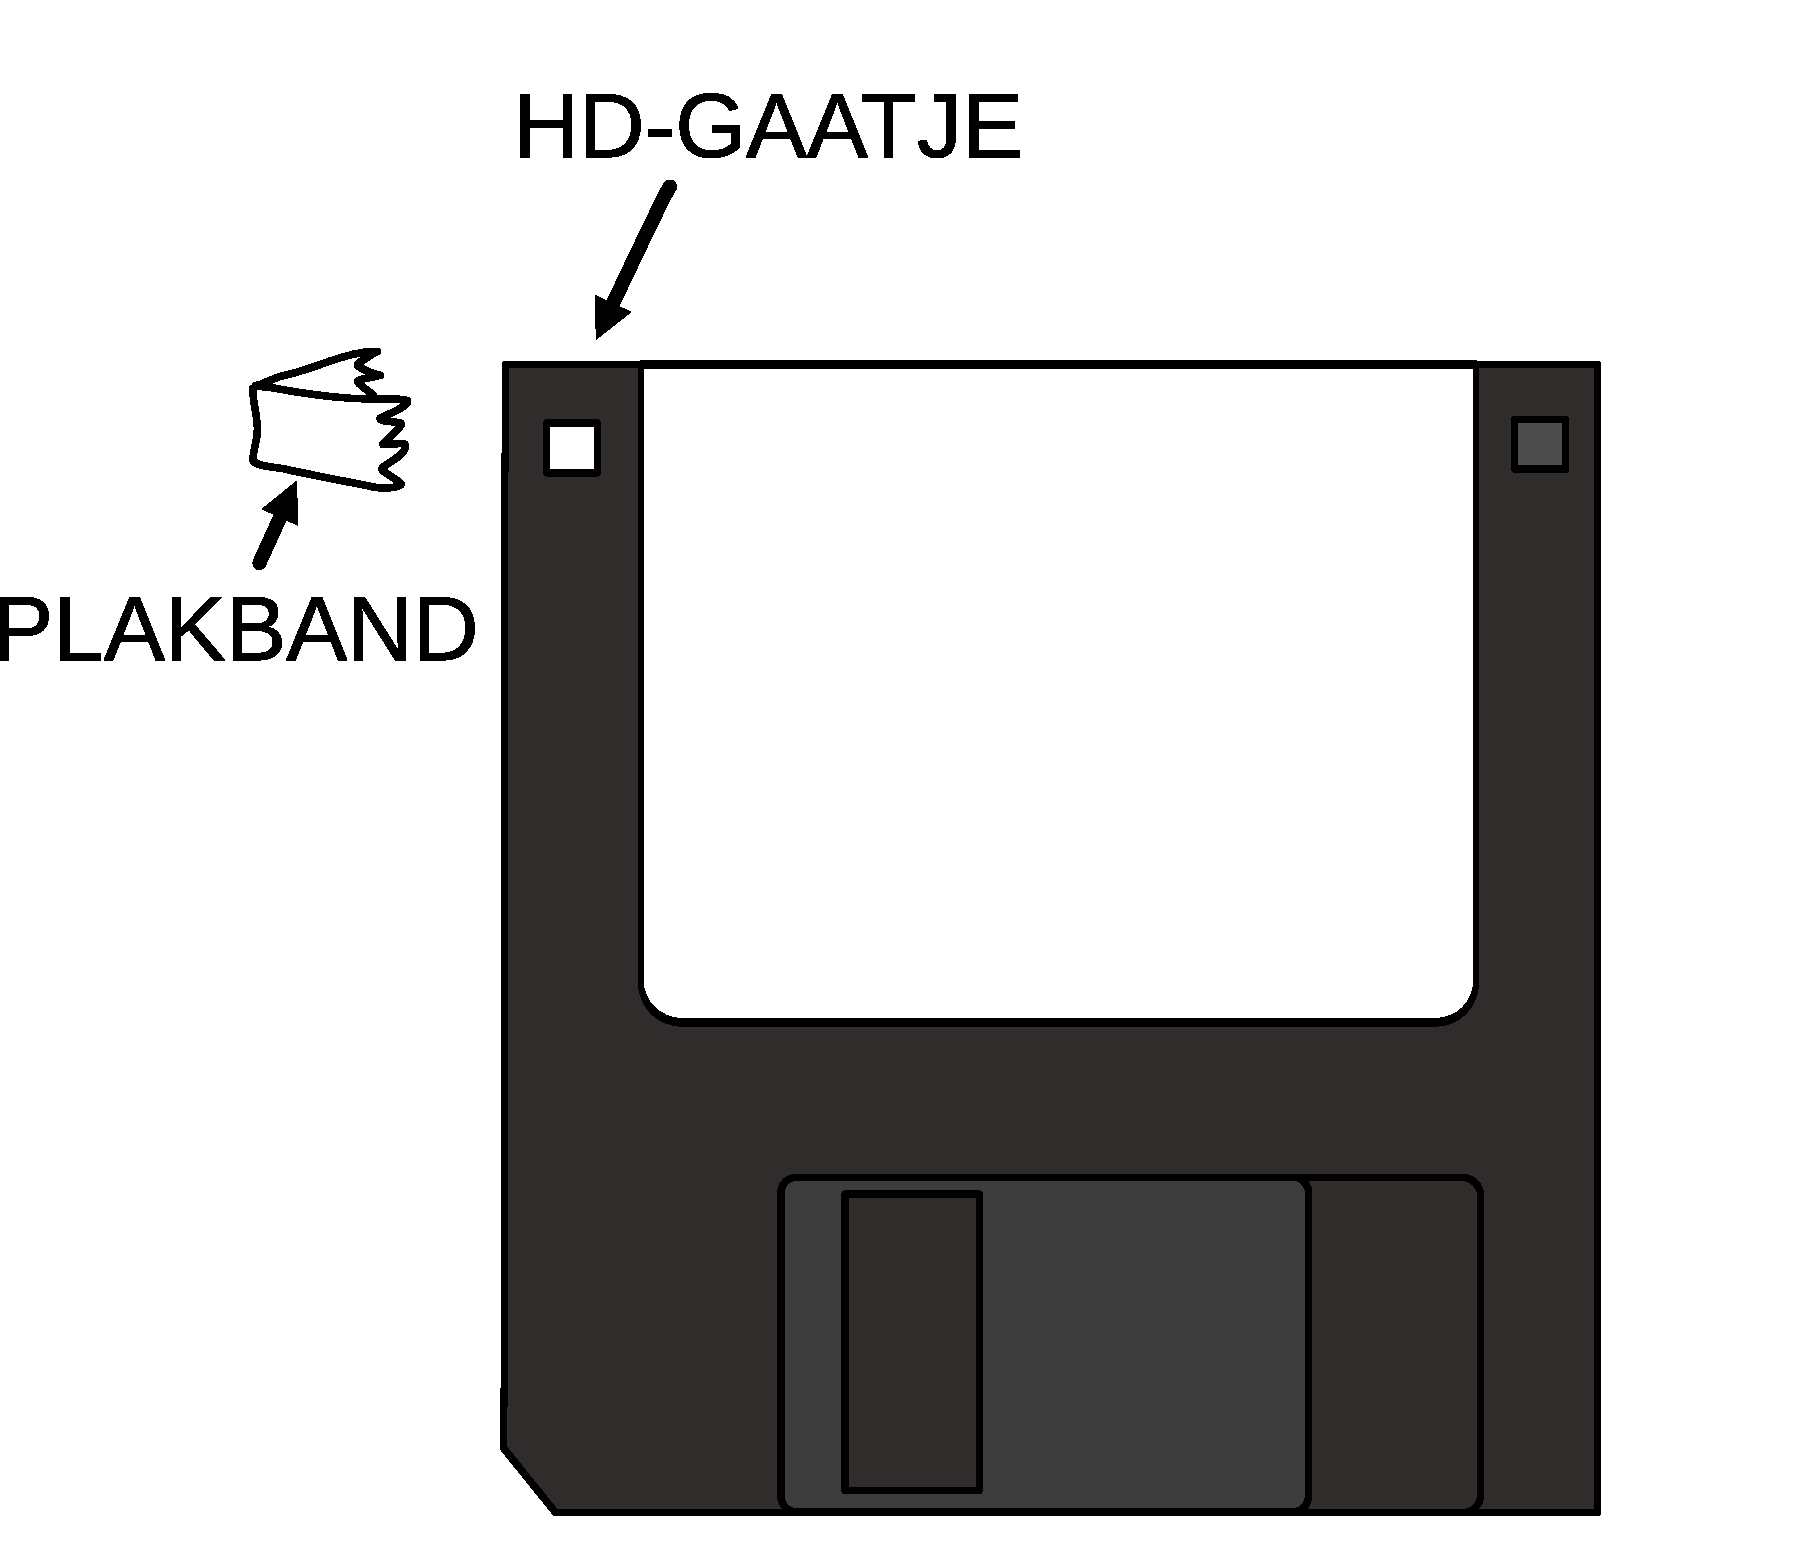
\includegraphics[width=0.75\textwidth]{dutch/images/illustrations/floppy_hd.pdf}
\end{center}

\underline{OPMERKING}: Zorg ervoor dat het plakband beide zijden van het gat bedekt.

\subsection{Een schijf formatteren}
\index{Schijfstations!Een schijf formatteren}

Een diskette moet geformatteerd worden voordat deze gebruikt kan worden. Het ingebouwde 3.5"-diskettestation van de MEGA65 emuleert een Commodore 1581-station en kan schijven gebruiken die in een dergelijk station zijn geformatteerd. U kunt een schijf ook met de MEGA65 formatteren.

\underline{OPMERKING}: Het formatteren van een schijf wist de inhoud ervan. Wees voorzichtig en doe dit uitsluitend wanneer u de gegevens op de schijf niet meer nodig hebt!

Voer de volgende stappen uit om een fysieke 3.5"-diskette met het interne station te formatteren:

\begin{enumerate}
\item Open het Freezer-menu.\index{Freezer-menu}\item Koppel het ingebouwde 3.5"-diskettestation aan het eerste beheerde station, unit 8.\item {\it Controleer dat unit 8 het volgende aangeeft:} \screentext{- INTERNAL 3.5" -}\item Hervat de computer: druk op \megakey{F3}.\item Plaats de diskette die u wilt formatteren in het interne diskettestation.\item Voer het BASIC-commando {\bf FORMAT} in en geef de schijf een naam ({\tt "MIJNDISK"}) en een ID van twee tekens ({\tt XX}).\index{BASIC 65-commando's!FORMAT}\index{BASIC 65-voorbeelden!FORMAT}
\begin{screencode}
FORMAT "MIJNDISK",IXX
\end{screencode}
\item Voer, wanneer u daarom gevraagd wordt, {\tt YES} in en druk op \widekey{RETURN}.
\end{enumerate}

Het formatteren van de schijf duurt ongeveer een minuut. Het station maakt tijdens het formatteren zoemende en klikkende geluiden. Schakel de computer niet uit en werp de schijf niet uit voordat het formatteren is voltooid.

U kunt bevestigen dat het formatteren is geslaagd door het {\bf DIR}-commando uit te voeren.\index{BASIC 65-commando's!DIR} U ziet dan een lege lijst van mappen met de naam en de ID die u hebt opgegeven. Uw schijf is nu gereed voor gebruik.


\section{Externe IEC-schijfstations gebruiken}
\index{Aansluitingen!IEC}

De MEGA65 werkt met externe schijfstations die op de seriële IEC-poort zijn aangesloten.

Externe stations hoeven niet te worden gekoppeld. Indien een unitnummer niet aan het ingebouwde 3.5"-diskettestation of aan een schijfimage is toegewezen, worden de schijfbewerkingen voor dat unitnummer naar de seriële IEC-poort verzonden. Het is aan het apparaat dat op de poort is aangesloten om zijn unitnummer te herkennen. Sommige IEC-apparaten hebben schakelaars waarmee u het unitnummer kunt instellen. Andere werken alleen met een specifiek nummer.

Indien u een extern station hebt dat een specifiek unitnummer verwacht, moet u ervoor zorgen dat de MEGA65 dat nummer niet aan een schijfimage of aan het interne station toewijst. Open het Freezer-menu\index{Freezer-menu} en druk vervolgens op \megakey{8} of \megakey{9} om de unitnummertoewijzingen om te schakelen, zodat zij het benodigde unitnummer niet meer gebruiken.\index{Unitnummer (IEC-apparaten)}

De station- en unitnummertoewijzingen zijn tijdelijk en worden teruggezet op hun standaardwaarden wanneer de MEGA65 wordt uitgeschakeld. U zult de stationtoewijzingen opnieuw moeten instellen wanneer u de computer de volgende keer inschakelt.


\section{Opstartbare schijven}
\index{Schijfstations!Opstartbare schijven}

Bij oudere Commodore-computers was het gebruikelijk dat softwaremakers de map op een diskette zo organiseerden dat het eerste bestand in de lijst het hoofdprogramma is. De gebruiker kon dan het commando \screentext{LOAD "*",8,1} invoeren om het hoofdprogramma te laden en \screentext{RUN} om het uit te voeren. Het sterretje is een jokerteken dat met elk bestand overeenkomt, dus ook met het eerste bestand op de schijf, zonder dat de gebruiker de naam van het programma hoeft te typen.

Deze methode is nog steeds gebruikelijk en de MEGA65 biedt een snelle manier om dergelijke schijven op te starten: houd \specialkey{SHIFT} ingedrukt en druk op \specialkey{RUN\\STOP}. Dit voert het commando \screentext{RUN "*"} uit, hetwelk vergelijkbaar is met de bekende commandoreeks die het eerste programma op de schijf laadt en uitvoert.\index{BASIC 65-commando's!RUN}

Met de C65 introduceerde Commodore een nieuwe manier om schijven op te starten. In plaats van te vertrouwen op de volgorde van bestanden, kan een schijf een bestand bevatten met de naam {\tt AUTOBOOT.C65}.\index{AUTOBOOT.C65-bestand} Indien dit bestand bestaat en een programma is, laadt en voert het BASIC-commando {\bf BOOT} dit bestand uit.\index{BASIC 65-commando's!BOOT}\index{BASIC 65-voorbeelden!BOOT}

\begin{screencode}
BOOT
\end{screencode}

\subsection{Schijven automatisch opstarten}

Zoals besproken in hoofdstuk \vref{cha:configuringyourmega}, kunt u het Configuratiehulpprogramma\index{Configuratie!Hulpprogramma} gebruiken om de MEGA65 in te stellen zodat hij tijdens het opstarten automatisch een virtueel schijfimage of het ingebouwde 3.5"-diskettestation koppelt.

Indien de gekoppelde schijf opstartbaar is --- dat wil zeggen dat hij een programmabestand met de naam {\tt AUTOBOOT.C65} bevat --- laadt en voert de MEGA65 het opstartprogramma automatisch uit.

Zo werkt de Intro Disk. Het Intro Disk-menu is een programma met de naam {\tt AUTOBOOT.C65} op het virtuele schijfimage {\tt MEGA65.D81}, hetwelk vooraf is ingesteld om bij het opstarten van het systeem gekoppeld te worden. Wanneer u de Intro Disk via het menu uitschakelt, hernoemt hij {\tt AUTOBOOT.C65} naar {\tt MENU}, zodat de schijf niet langer als opstartbaar wordt beschouwd.

Zelf een opstartschijf inrichten is een handige manier om uw computer te configureren. U kunt een kort BASIC-programma schrijven dat het systeemlettertype wijzigt, de achtergrondkleur aanpast en {\bf KEY}-macro's naar uw smaak instelt. Sla dit programma vervolgens op als {\tt AUTOBOOT.C65} op een schijf die u hebt geconfigureerd om bij het opstarten van het systeem aan te koppelen. Dit programma wordt elke keer uitgevoerd wanneer u uw MEGA65 inschakelt.


\section{De SD-kaart benaderen vanuit BASIC}

Verscheidene BASIC 65-commando's kunnen rechtstreeks op de SD-kaart van de MEGA65 werken alsof deze een schijfstation is. In deze gevallen staat de SD-kaart bekend als unit 12.

\underline{OPMERKING}: Unit 12 kan slechts voor enkele specifieke bewerkingen rechtstreeks worden benaderd. Hij kan de gehele SD-kaart niet als een CBDOS-schijf behandelen.

Om alle bestanden op de SD-kaart weer te geven, gebruikt u het {\bf DIR}-commando met het argument \screentext{U12}:\index{BASIC 65-commando's!DIR}\index{BASIC 65-voorbeelden!DIR}

\begin{screencode}
DIR U12
\end{screencode}

U kunt de optionele {\bf P}-vlag met dit commando gebruiken om de bestanden op de SD-kaart één pagina tegelijk weer te geven. Druk op Q om op de huidige pagina te stoppen, of op een willekeurige andere toets om naar de volgende pagina te gaan.

\begin{screencode}
DIR U12,P
\end{screencode}

Om een PRG-bestand rechtstreeks van de SD-kaart te laden (dat zich niet in een schijfimage bevindt), gebruikt u het \screentext{U12}-argument bij het {\bf DLOAD}-commando. In dit geval {\em moet} u het achtervoegsel {\tt .PRG} van de bestandsnaam opnemen, hetgeen verschilt van het gebruik van PRG-bestanden op schijven of in schijfimages. {\bf DSAVE} kan niet naar de SD-kaart opslaan met \screentext{U12} en meldt een fout als u het toch probeert; sla een programma daarom op in een schijfimage.\index{BASIC 65-commando's!DLOAD}\index{BASIC 65-commando's!DSAVE}\index{BASIC 65-voorbeelden!DLOAD}

\begin{screencode}
DLOAD "MIJNPROGJE.PRG",U12
\end{screencode}

Zoals eerder is besproken, ondersteunt de MEGA65 submappen op de SD-kaart en houdt een huidige werkmap bij voor schijfbewerkingen. Om de huidige werkmap te wijzigen naar een submap:\index{BASIC 65-commando's!CHDIR}\index{BASIC 65-voorbeelden!CHDIR}

\begin{screencode}
CHDIR "SUBDIR",U12
\end{screencode}

Om de huidige werkmap te wijzigen naar de bovenliggende map:

\begin{screencode}
CHDIR "..",U12
\end{screencode}

Het {\bf MOUNT}-commando kan een D81- of D64-schijfimage aan een unitnummer koppelen. Hoewel dit commando naar een bestand op de SD-kaart verwijst, maakt het geen gebruik van het \screentext{U12}-argument. In plaats daarvan stelt het commando met het {\bf U}-argument het unitnummer van de aan te koppelen schijf in. Het {\bf MOUNT}-commando gebruikt de door {\bf CHDIR} ingestelde huidige werkmap om het bestand te vinden.


\section{Gangbare schijfbewerkingen}

Hieronder vindt u enkele voorbeelden van gangbare schijfbewerkingen die u bij de \screentext{READY}-prompt kunt uitvoeren. Raadpleeg voor meer informatie de naslag over BASIC-commando's in bijlage \vref{cha:basic-reference}.

De meeste commando's die bestandsnamen aanvaarden, aanvaarden ook een {\bf U}-argument waarmee u aangeeft welke unit het bestand bevat. De standaardunit is 8.\footnote{Wanneer de computer voor het eerst wordt gestart, is de standaard schijfunit voor BASIC-commando's 8. U kunt deze wijzigen met het {\bf SET DEF}-commando.\index{BASIC 65-commando's!SET}}

\subsection{DIR}
\index{BASIC 65-commando's!DIR}\index{BASIC 65-voorbeelden!DIR}

Om de map (de lijst van bestanden) van een schijf weer te geven, gebruikt u het {\bf DIR}-commando.

\begin{screencode}
DIR

DIR U9
\end{screencode}

In tegenstelling tot de methode van de Commodore 64, waarbij de schijfmap in het BASIC-geheugen wordt geladen, wijzigt het {\bf DIR}-commando het BASIC-geheugen niet. U kunt {\bf DIR} veilig gebruiken wanneer er een programma in het geheugen staat.

Om grotere mappen gemakkelijker te kunnen bekijken, geeft {\bf DIR W} (van ``wide'') de map in kolommen weer en pauzeert na elke pagina.

\subsection{DLOAD en RUN}
\index{BASIC 65-commando's!DLOAD}\index{BASIC 65-voorbeelden!DLOAD}
\index{BASIC 65-commando's!RUN}\index{BASIC 65-voorbeelden!RUN}

Het {\bf DLOAD}-commando laadt een programma van de schijf in het geheugen. Het {\bf RUN}-commando voert het programma uit dat zich momenteel in het geheugen bevindt.

\begin{screencode}
DLOAD "GAAFSPEL"
RUN
\end{screencode}

U kunt beide tot één commando combineren door de bestandsnaam rechtstreeks aan het {\bf RUN}-commando te geven.

\begin{screencode}
RUN "GAAFSPEL"
\end{screencode}

\subsection{DSAVE}
\index{BASIC 65-commando's!DSAVE}\index{BASIC 65-voorbeelden!DSAVE}

Het {\bf DSAVE}-commando slaat het BASIC-programma dat zich momenteel in het geheugen bevindt op de schijf op.

\begin{screencode}
DSAVE "MIJNSPEL"
\end{screencode}

Standaard overschrijft dit geen bestaand bestand met dezelfde naam. Om een bestaand bestand te laten overschrijven, plaatst u een apestaartje vóór de bestandsnaam, binnen de dubbele aanhalingstekens.

\begin{screencode}
DSAVE "@MIJNSPEL"
\end{screencode}

Merk op dat opslaan met vervanging alleen wordt aanbevolen bij gebruik van schijfimages en het 3.5"-diskettestation. Oudere Commodore-stations bevatten fouten in deze functie die tot gegevensverlies kunnen leiden.

\subsection{BACKUP}
\index{BASIC 65-commando's!BACKUP}\index{BASIC 65-voorbeelden!BACKUP}

Het {\bf BACKUP}-commando kopieert een volledige schijf van de ene unit naar de andere. Hierbij worden alle bestaande gegevens op de bestemmingsschijf gewist.

\begin{screencode}
BACKUP U8 TO U9
\end{screencode}

U kunt {\bf BACKUP} gebruiken om schijfimages van floppy-schijven te maken, schijfimages naar floppy-schijven te schrijven of alles van het ene schijfstation naar het andere te kopiëren.

\subsection{COPY}
\index{BASIC 65-commando's!COPY}\index{BASIC 65-voorbeelden!COPY}

Het {\bf COPY}-commando maakt een kopie van een bestand. Indien bron en bestemming verschillende bestandsnamen op dezelfde unit zijn, dupliceert dit het bestand op de schijf. Wanneer u een bestand tussen units kopieert, behoudt het bestand zijn oorspronkelijke bestandsnaam. (Het nieuwe bestand kan met een afzonderlijk commando worden hernoemd.)

\begin{screencode}
COPY "MIJNSPEL", U8 TO U9

COPY "MIJNSPEL" TO "MIJNSPEL-V1"
\end{screencode}

\subsection{RENAME}
\index{BASIC 65-commando's!RENAME}\index{BASIC 65-voorbeelden!RENAME}

Het {\bf RENAME}-commando wijzigt de naam van een bestaand bestand.

\begin{screencode}
RENAME "MIJNSPEL-V29" TO "MIJNSPEL-GEREED"
\end{screencode}

\subsection{DELETE}
\index{BASIC 65-commando's!DELETE}\index{BASIC 65-voorbeelden!DELETE}

Het {\bf DELETE}-commando verwijdert een bestand.

\begin{screencode}
DELETE "ROMMELBESTAND"
\end{screencode}


\subsection{Snelkoppelingen voor schijfcommando's}

BASIC 65 biedt enkele snelkoppelingen voor gangbare schijfcommando's die u bij de \screentext{READY}-prompt kunt gebruiken.

\begin{center}
\begin{tabular}{|l|l|}
\hline
{\bf Snelkoppeling} & {\bf Overeenkomend commando} \\
\hline
\screentextwide{/} & {\bf LOAD} \\
\hline
$\uparrow$ & {\bf RUN} \\
\hline
$\leftarrow$ & {\bf SAVE} \\
\hline
\screentextwide{@} & {\bf DISK} \\
\hline
\screentextwide{\$} & {\bf DIR} \\
\hline
\end{tabular}
\end{center}

Deze snelkoppelingen zijn bedoeld om samen met een lijst van mappen programma's te starten zonder dat u bestandsnamen hoeft te typen. Bijvoorbeeld:

\begin{enumerate}
\item Geef de lijst van mappen van de schijf weer: typ {\bf \$} in en druk op \widekey{RETURN}.\item Gebruik de cursortoetsen om de cursor te verplaatsen naar de regel met het programma dat u wilt uitvoeren.\item Typ {\bf \screentext{$\uparrow$}} in en druk op \widekey{RETURN}.
\end{enumerate}

Het geselecteerde programma wordt geladen en uitgevoerd. Merk op dat u geen overtollige tekens van de regel hoeft te verwijderen. De snelkoppeling negeert alles behalve de bestandsnaam tussen dubbele aanhalingstekens, zoals die door de lijst van mappen wordt weergegeven.

\chapter{Bestanden overzetten}

\section{Bestanden naar de MEGA65 overbrengen}
\label{cha:transferring-files}
\index{SD-kaarten!Bestanden overzetten}

Het schrijven van uw eigen programma's voor de MEGA65 is erg leuk, maar uiteindelijk wilt u ook programma's uitvoeren die door anderen zijn geschreven. Wellicht wilt u ook een reservekopie van uw MEGA65-programma's op uw pc maken om ze veilig te bewaren.

De snelste en betrouwbaarste manier om bestanden tussen uw pc en uw MEGA65 over te zetten is met een Ethernet-kabel.\index{Netwerk!Ethernet} U sluit het ene uiteinde van de kabel aan op de RJ45-aansluiting aan de achterzijde van de MEGA65. U kunt het andere uiteinde aansluiten op de router of switch van uw local area network (LAN), of rechtstreeks op uw pc. U gebruikt software op uw pc om bestandsoverdrachten in beide richtingen te starten: van de pc naar de MEGA65 of van de MEGA65 naar de pc.

Als alternatief kunt u D81-virtuele schijfimages met behulp van een willekeurige pc met een SD-kaartlezer naar uw door de MEGA65 geformatteerde SD-kaart kopiëren, zonder andere speciale hulpmiddelen of software. Uw pc herkent het gegevensgebied van de SD-kaart als een FAT32-partitie. Indien u deze methode gebruikt, dient u zich ervan bewust te zijn dat sommige besturingssystemen van pc's ongewenste neveneffecten kunnen hebben, zoals fragmentatie van bestanden op de SD-kaart of overbodige bestanden die door macOS Finder worden aangemaakt. Deze effecten zijn onschadelijk voor de gegevens, maar kunnen onderhoud vergen om de kaart bruikbaar te houden in de MEGA65. Indien de MEGA65 meldt dat een bestand gefragmenteerd is, kunt u op de gegevenspartitie een defragmentatiehulpmiddel voor pc-schijven gebruiken. Als alternatief kunt u alle bestanden van de SD-kaart naar de pc kopiëren, de SD-kaart in de MEGA65 opnieuw formatteren en de bestanden vervolgens vanaf de pc terugkopiëren.

Het is ook mogelijk om bestanden over te zetten via een JTAG- of UART seriële interface die op het moederbord is aangesloten. Dit is een geavanceerde techniek en wordt niet in deze gebruikershandleiding beschreven. JTAG- of UART Serial-hardware biedt toegang tot een debuginterface die voor sommige programmeurs nuttig kan zijn. JTAG is ook nuttig voor het ontwikkelen van FPGA-cores. Zie voor meer informatie {\it De Mega65 programmeergids.}

De meeste mensen geven de voorkeur aan de Ethernet-methode. Dit hoofdstuk beschrijft hoe u dat doet.

\section{Netwerken begrijpen}

De MEGA65 kan Ethernet gebruiken om verbinding te maken met andere computers in een netwerk, of om verbindingen van andere computers te aanvaarden. Met de juiste programmatuur kan hij via het internet verbinding maken met andere computers.

De Ethernet-hardware van de MEGA65 biedt het lokale netwerk een Media Access Control (MAC)-adres aan.\index{Netwerk!MAC-adres} In tegenstelling tot andere Ethernet-hardware wordt het MAC-adres van de MEGA65 niet in de fabriek toegewezen: het wordt ingesteld in het configuratiehulpprogramma. (Zie hoofdstuk \vref{cha:configuringyourmega}.)

Om bestanden over te zetten, geeft u de MEGA65 opdracht zich beschikbaar te stellen voor binnenkomende verbindingen. Vervolgens gebruikt u op uw pc de M65Connect-app (of een ander hulpprogramma, zoals \texttt{mega65\_ftp}) om een verbinding tot stand te brengen. Het besturingssysteem van uw pc kan om toestemming vragen om het hulpprogramma toegang tot het netwerk te verlenen wanneer u het voor de eerste keer uitvoert. Het hulpmiddel gebruikt UDP-poort 4510 om de eerste verbinding met de MEGA65 tot stand te brengen en gebruikt voor de bestandsoverdrachtssessie een zelf toegewezen IPv6-adres dat op basis van het MAC-adres van de MEGA65 is aangemaakt. Hiervoor moet IPv6 op de netwerkinterface van de pc zijn ingeschakeld, wat in de meeste gevallen de standaardinstelling is.

Als alternatief voor de aansluiting op uw lokale netwerk kunt u de MEGA65, indien uw pc over een Ethernet-aansluiting beschikt, rechtstreeks met een Ethernet-kabel op uw pc aansluiten. Zo vormt u een klein lokaal netwerk zonder toegang tot het internet. De werkwijze voor het overzetten van bestanden is bij een rechtstreekse verbinding dezelfde als bij een verbinding via het lokale netwerk.

\section{M65Connect verkrijgen}
\index{M65Connect-toepassing}

{\bf M65Connect} is een toepassing voor Windows, Mac of Linux die bestandsoverdrachten en andere nuttige functies voor MEGA65-gebruikers mogelijk maakt. De toepassing beschikt over een interface met vensters en bevat tevens commandoregelhulpmiddelen die nuttig zijn bij het programmeren.

Om M65Connect te verkrijgen:

\begin{enumerate}
\item Bezoek de MEGA65 Filehost-website\index{Filehost-website} in een browser: \url{https://files.mega65.org}\item Typ in het zoekveld rechtsboven: ``M65Connect''\item Selecteer de versie van M65Connect voor het besturingssysteem van uw pc.\item Klik op de knop ``Download''.\item Gebruik uw pc om het gedownloade archiefbestand uit te pakken.
\end{enumerate}

\subsection{M65Connect voor Windows}

De Windows-versie van M65Connect staat in de map ``M65Connect'': {\bf M65Connect.exe}. Zoals bij de meeste openbronprogrammatuur het geval is, kan Microsoft Defender weigeren de programmatuur uit te voeren en een dialoogvenster weergeven. Indien dit gebeurt, klikt u op ``More info'' en vervolgens op de knop ``Run anyway'' die verschijnt.

De commandoregelhulpmiddelen staan in een submap met de naam ``M65Connect Resources'', zoals: {\tt M65Connect Resources\textbackslash{}mega65\_ftp.exe}

\subsection{M65Connect voor macOS}

De macOS-versie van M65Connect is een Mac-toepassingsbundel: {\bf M65Connect.app}. Zoals bij de meeste openbronprogrammatuur het geval is, beschouwt macOS het niet als door de ontwikkelaar ondertekend en zal macOS weigeren het uit te voeren. U moet het kenmerk ``quarantine'' verwijderen om de toepassing te kunnen uitvoeren.

In de meeste versies van macOS kunt u het quarantainekenmerk het eenvoudigst verwijderen met een Terminal-opdracht:

\begin{enumerate}
\item Verplaats de M65Connect-app naar uw map Applications.\item Open de Terminal-app, die bij macOS is inbegrepen. U vindt deze in de map Applications, in een submap met de naam Utilities.\item Voer deze opdracht in: {\tt xattr -cr /Applications/M65Connect.app}
\end{enumerate}

U kunt de M65Connect-app nu met een dubbelklik uitvoeren.

De commandoregelhulpmiddelen bevinden zich in de map van de toepassingsbundel, zoals: {\tt /Applications/M65Connect.app/Contents/Resources/mega65\_ftp.osx}

\subsection{M65Connect voor Linux}

De Linuxversie van M65Connect bevindt zich in de map ``M65Connect'': {\bf M65Connect}. Dubbelklik erop om het uit te voeren.

De commandoregelhulpmiddelen staan in een submap met de naam ``M65Connect Resources'', zoals: {\tt M65Connect Resources/mega65\_ftp}

\section{Netwerkluisteren inschakelen}
\index{Netwerk!Luistermodus}

Standaard negeert de MEGA65 alle pogingen van andere computers om er via het netwerk verbinding mee te maken. Programmatuur welke op de MEGA65 draait, kan luisteren naar netwerkverbindingen, doch de MEGA65 doet dit niet uit zichzelf.

Om bestanden met M65Connect over te zetten, dient u de MEGA65 te laten luisteren naar binnenkomende verbindingspogingen van M65Connect. Druk op \specialkey{SHIFT} + \megakey{\pounds} om een netwerkluistersessie in te schakelen. Het stroomlampje knippert afwisselend geel en groen wanneer netwerkluisteren actief is.

\begin{center}
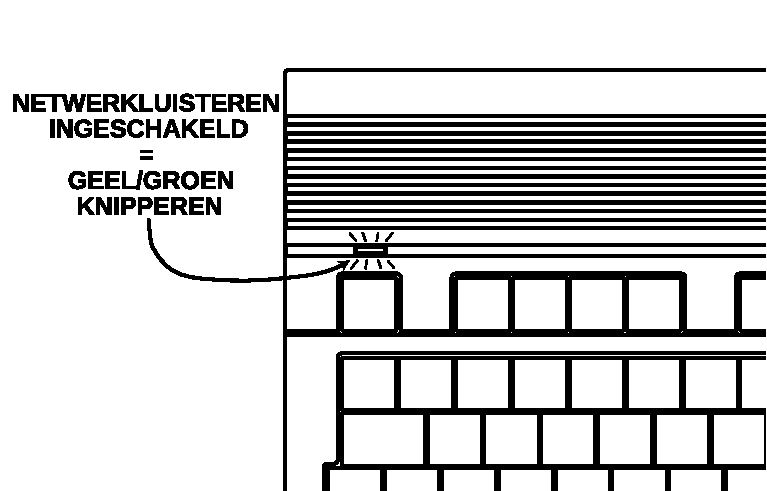
\includegraphics[width=\linewidth]{dutch/images/illustrations/mega65-eth-blink.pdf}
\end{center}

Druk opnieuw op \specialkey{SHIFT} + \megakey{\pounds} om netwerkluisteren uit te schakelen, of reset de computer.

Indien het stroomlampje na het indrukken van \specialkey{SHIFT} + \megakey{\pounds} niet begint te knipperen, moet u mogelijk DIP-schakelaar \#2 op het moederbord instellen. Bij MEGA65-modellen die in 2024 of later zijn gefabriceerd, hoort deze schakelaar in de fabriek ingesteld te zijn. Bij oudere MEGA65-modellen staat deze schakelaar standaard uit.

Om de DIP-schakelaar in te stellen,\index{DIP-schakelaars} opent u de behuizing zoals beschreven in hoofdstuk \vref{cha:setup}. Zoek de DIP-schakelaars op het moederbord en zet DIP-schakelaar \#2 in de positie ``on''. Zoek naar markeringen op de schakelaars om schakelaar \#2 en de richting ``on'' te herkennen. (De oriëntatie van uw DIP-schakelaars kan van dit diagram afwijken.)

\begin{center}
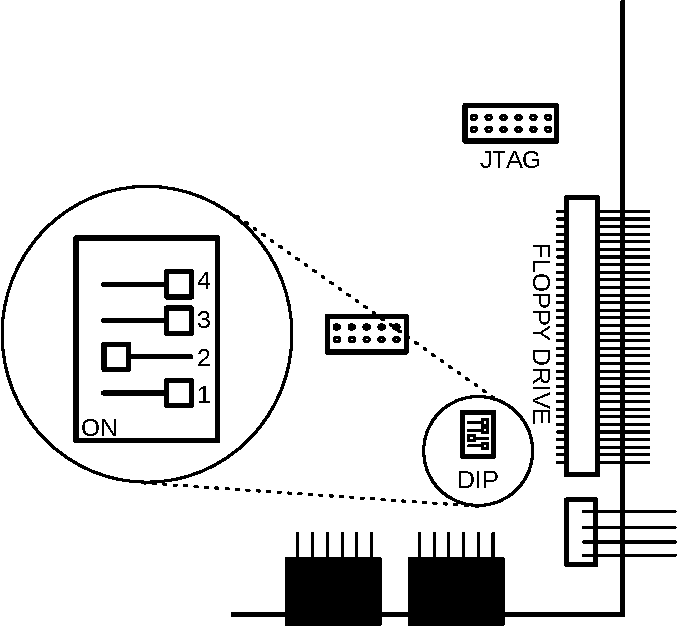
\includegraphics[width=\linewidth]{images/illustrations/mega65-dip2.pdf}
\end{center}

U kunt DIP \#2 gerust in deze positie laten staan voor normaal gebruik.


\section{Bestanden overzetten}

Om bestanden over te zetten, start u een bestandsoverdrachtssessie met de toepassing M65Connect of het commandoregelhulpmiddel {\tt mega65\_ftp}. Dit hulpmiddel maakt verbinding met de MEGA65 en uploadt een bestandsoverdrachtclient voor gebruik tijdens de sessie. Wanneer u de sessie beëindigt, reset de MEGA65.

Het starten van een bestandsoverdrachtssessie reset de MEGA65. Sla eventuele programma's of gegevens op voordat u verdergaat.

\underline{OPMERKING}: Indien u het geheugen wist door de computer te resetten, vergeet dan niet om netwerkluisteren opnieuw in te schakelen: druk op \specialkey{SHIFT} + \megakey{\pounds} en zorg dat het stroomlampje knippert.

\subsection{Bestanden overzetten met M65Connect}
\index{M65Connect-toepassing}

M65Connect detecteert automatisch of de MEGA65 naar verbindingen luistert. Open M65Connect en schakel vervolgens de netwerkluistersessie op de MEGA65 in. M65Connect meldt een status van "Connected to MEGA65 via LAN". M65Connect schakelt daarna in het venster diverse knoppen in, waaronder de {\bf PRG}- en {\bf SD Card}-knoppen.

\begin{center}
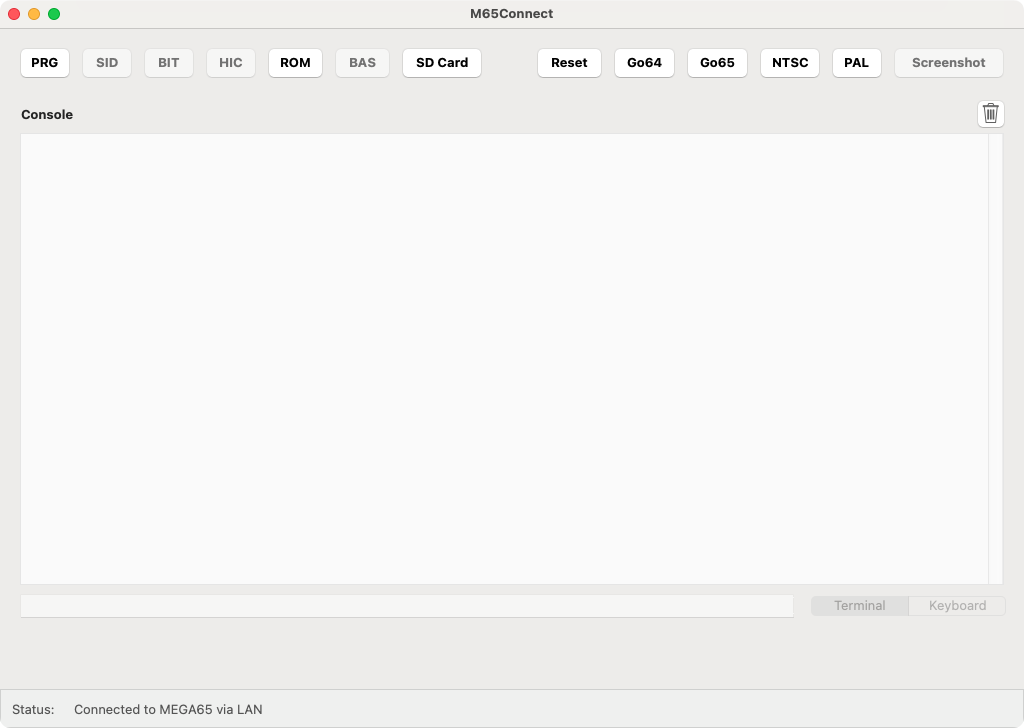
\includegraphics[width=\linewidth]{images/m65connect_macos.png}
\end{center}

Indien M65Connect een status van "Not connected to MEGA65" meldt, controleer dan het volgende:

\begin{itemize}
\item De MEGA65 en de pc zijn op hetzelfde netwerk aangesloten of rechtstreeks op elkaar via een netwerkkabel.\item De MEGA65 bevindt zich in de netwerkluistermodus met een knipperend stroomlampje.\item Open in M65Connect het menu Settings en selecteer Connections. Het veld "LAN Port" hoort een IPv6-adres te bevatten. Indien dat niet het geval is, wacht dan enkele seconden of klik op de knop "Autodetect LAN Port".
\end{itemize}

Klik op de knop {\bf SD Card} om een bestandsoverdrachtssessie te starten. Het SD Card Manager-venster gaat open.

\underline{OPMERKING}: Het starten van een bestandsoverdrachtssessie reset de MEGA65 om het bestandsoverdrachtshulpprogramma te laden. Zorg ervoor dat u eventuele gegevens op de MEGA65 hebt opgeslagen voordat u de sessie start.

\begin{center}
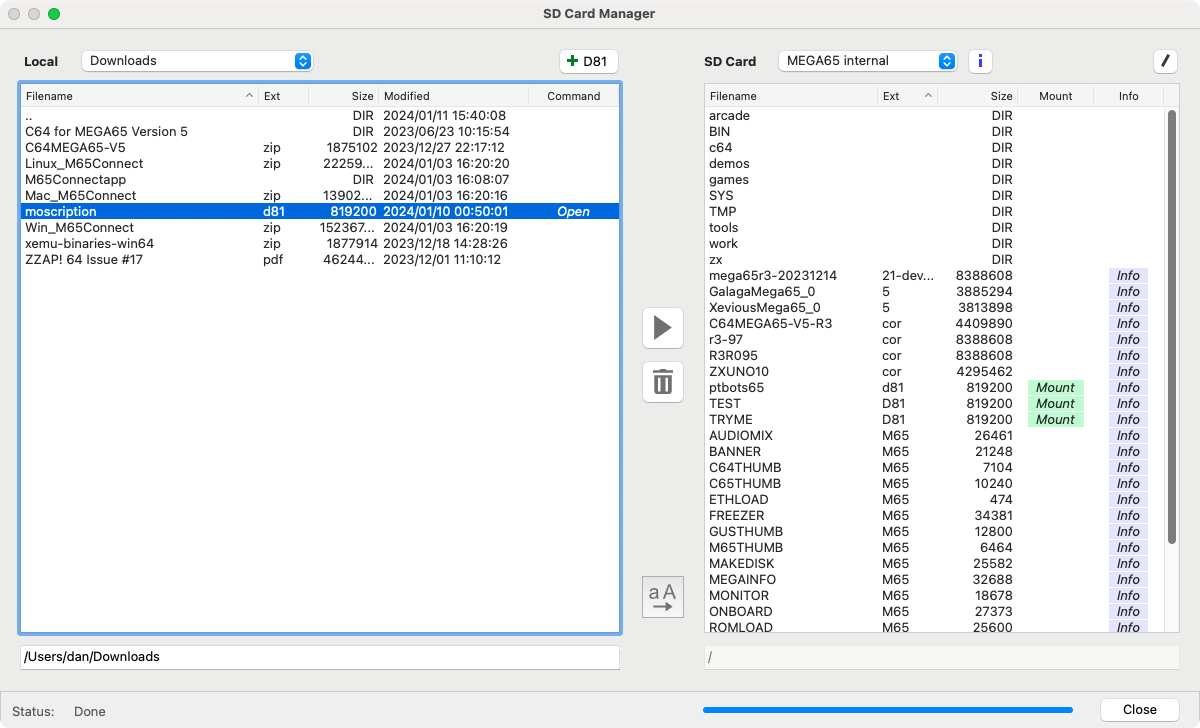
\includegraphics[width=\linewidth]{images/m65connect_files.png}
\end{center}

Gebruik het linkerdeelvenster om door de bestanden op uw pc te navigeren en het rechterdeelvenster om door de bestanden op de SD-kaart van de MEGA65 te navigeren. Selecteer het bestand en klik daarna op de pijlknop om het over te zetten. De knop geeft de richting aan waarin het bestand wordt overgezet.

U kunt M65Connect ook gebruiken om D81-schijfimages aan te maken en bestanden van en naar D81-schijfimages te kopiëren. Zoek een D81-schijfimage op uw pc of klik op de knop {\bf + D81} om er een aan te maken. Klik daarna in de bestandsverkenner op de opdracht "Open" om het schijfimage in het linkerdeelvenster te openen. Zet bestanden met de pijlknop over van en naar het schijfimage. Klik op de knop {\bf X} in de rechterbovenhoek om terug te keren naar de bestandsverkenner.

Klik op de knop {\bf Close} om de bestandsoverdrachtssessie te beëindigen en het SD Card Manager-venster te sluiten. Dit reset de MEGA65.

\subsection{Het commandoregelhulpmiddel mega65\_ftp}
\index{mega65\_ftp-commando@\texttt{mega65\_ftp-commando}}

Het commandoregelhulpmiddel {\tt mega65\_ftp} start een bestandsoverdrachtssessie met de MEGA65. Het kan interactief in de terminal draaien en meerdere bestandsoverdrachtopdrachten aanvaarden, of niet-interactief draaien met deze opdrachten als argumenten.

Om een interactieve bestandsoverdrachtssessie te starten, voert u de opdracht {\tt mega65\_ftp} uit en geeft u daarbij het argument {\tt -e} mee om aan te geven dat u een Ethernet-verbinding wilt gebruiken.

\underline{OPMERKING}: Het starten van een bestandsoverdrachtssessie reset de MEGA65 om het bestandsoverdrachtshulpprogramma te laden. Zorg ervoor dat u eventuele gegevens op de MEGA65 hebt opgeslagen voordat u de sessie start.

\begin{verbatim}
% mega65_ftp -e
\end{verbatim}

Het hulpprogramma uploadt de bestandsoverdrachtclient en u ziet de client op de MEGA65 draaien. Indien er niets gebeurt, drukt u op Ctrl-C (op de pc) om de overdracht af te breken en controleert u daarna nogmaals of de MEGA65 verbonden is en of netwerkluisteren is ingeschakeld.

Zodra de verbinding tot stand is gekomen, ziet de prompt voor bestandsoverdrachtopdrachten er ongeveer zo uit:

\begin{verbatim}
MEGA65 SD-Card:/>
\end{verbatim}

Om de sessie te beëindigen, gebruikt u de opdracht {\tt exit}. Het hulpprogramma sluit af, u keert terug naar de shellprompt en de MEGA65 reset.

\begin{verbatim}
MEGA65 SD-Card:/> exit
%
\end{verbatim}

Hieronder volgen enkele nuttige opdrachten die u tijdens de bestandsoverdrachtssessie kunt gebruiken. Gebruik de opdracht {\tt help} om een volledige lijst van de beschikbare opdrachten te zien.

\begin{center}
\begin{tabular}{|l|l|}
\hline
{\bf Opdracht} & {\bf Omschrijving} \\
\hline
{\tt put {\it bestandsnaam}} & Verstuurt een bestand van de pc naar de MEGA65. \\
\hline
{\tt get {\it bestandsnaam}} & Haalt een bestand op van de MEGA65 en plaatst het op de pc. \\
\hline
{\tt dir} & Toont een lijst van de mappen van de SD-kaart van de MEGA65. \\
\hline
{\tt ldir} & Toont een lijst van de huidige lokale werkmap. \\
\hline
{\tt mkdir {\it bestandsnaam}} & Maakt een submap aan op de SD-kaart van de MEGA65. \\
\hline
{\tt cd {\it bestandsnaam}} & Wijzigt de huidige werkmap op de SD-kaart van de MEGA65. \\
\hline
{\tt lcd {\it bestandsnaam}} & Wijzigt de huidige lokale werkmap. \\
\hline
{\tt help} & Toont een lijst met beschikbare opdrachten. \\
\hline
{\tt exit} & Beëindigt de bestandsoverdrachtssessie. \\
\hline
\end{tabular}
\end{center}

Om opdrachten van {\tt mega65\_ftp} aan te roepen zonder een interactieve prompt te starten, geeft u het argument {\tt -c} één keer per opdracht mee:

\begin{verbatim}
% mega65_ftp -e -c 'put mydisk.d81' -c 'exit'
\end{verbatim}

Het hulpprogramma start een sessie, voert de opdrachten uit en stopt vervolgens. Zorg ervoor dat u de opdracht {\tt exit} als laatste opdracht invoert om de MEGA65 te resetten, of reset de MEGA65 handmatig nadat de bestandsoverdracht is voltooid.

\part{EERSTE STAPPEN IN HET PROGRAMMEREN}

\chapter{Hoe computers werken}

Wist u dat veel computerexperts en programmeurs al leerden omgaan met computers toen ze nog kleine kinderen waren? Thuiscomputers werden pas in het begin van de jaren tachtig gemeengoed. Ze waren toen zo nieuw dat mensen vaak zelf programma's schreven om te doen wat zij wilden doen, omdat er nog geen software bestond die dat werk voor hen deed.

Het was ook heel gewoon dat mensen met allerlei kantoorbanen leerden programmeren op de computers die zij voor hun werk gebruikten. Zo leerden bijvoorbeeld de mensen die de salarisadministratie van een bedrijf deden, de computer te programmeren zodat die het salaris van iedereen berekende!

Sindsdien is er veel veranderd. De meeste mensen kiezen tegenwoordig bestaande programma's of toepassingen om te doen wat zij nodig hebben en denken dat programmeren een gespecialiseerde vaardigheid is die slechts sommige mensen kunnen leren. Dat is echter niet waar. Natuurlijk is iedereen, net als in elk ander vakgebied, in sommige dingen beter dan in andere, of het nu om sport, breien, wiskunde of schrijven gaat. Bijna iedereen is in staat genoeg te leren om zich in het leven te kunnen redden.

Wij hebben de MEGA65 gemaakt, omdat wij ervan overtuigd zijn dat juist u kunt leren programmeren, zodat computers nuttiger voor u worden, en dat u, net als bij het aanleren van elke nieuwe vaardigheid, de voldoening, het plezier en de nieuwe avonturen kunt ervaren die dat met zich meebrengt!


\phantomsection
\section{Computers zijn dom. Echt dom}

Hoe kan dit nu waar zijn? Computers kunnen zoveel verschillende dingen doen, vaak duizenden malen sneller dan een mens dat kan. Hoe kunnen wij dan beweren dat computers dom zijn? Het antwoord is dat geen enkele computer iets kan doen wat een persoon hem niet heeft opgedragen. Zelfs aan de nieuwste kunstmatige-intelligentiesystemen heeft men geleerd hoe zij moeten leren (of hoe zij moeten leren, hoe zij moeten leren). Om te begrijpen waarom dit zo is, helpt het om te begrijpen hoe computers werkelijk werken.

\subsection{Een eierdopjescomputer maken}

Het hart van een computer is de Central Processing Unit (CPU). Veel moderne computers hebben meer dan één processor, maar laten we het om te beginnen eenvoudig houden. De processor heeft een reeks eenvoudige instructies die hij begrijpt, zoals ``haal het ding uit eierdopje \#21'', ``stop dit ding in eierdopje \#403'', ``tel deze dingen bij elkaar op'' of ``voer de volgende instructie uit, maar alleen als het ding in eierdopje \#712 het getal 3 is.''

Wat bedoelen we eigenlijk met al die ``dingen'' en ``eierdopjes''? Laten we beginnen met na te denken over hoe we ons als computer kunnen voordoen, met niets meer dan een lege eierdoos, wat kleine papiertjes en een potlood of pen. Schrijf eerst in elk van de kleine eierdopjes van de eierdoos een getal, te beginnen bij één. Schrijf daarna het getal nul op een klein papiertje en leg dat papiertje in het eerste eierdopje. Doe hetzelfde voor de andere eierdopjes. U heeft nu een eierdoos met genummerde eierdopjes, waarin elk eierdopje een papiertje bevat waarop het getal nul staat. Nu hoeven we alleen nog een paar eenvoudige regels te bedenken die beschrijven hoe onze eierdopjescomputer werkt:

\begin{itemize}
  \item Ten eerste mag elk eierdopje precies één papiertje tegelijk bevatten. Nooit meer. Nooit minder. Zo weten we zeker dat er, wanneer we de vraag stellen ``wat zit er in eierdopje zoveel'', één eenduidig antwoord is. Zo werkt ook het computergeheugen: elke geheugenlocatie kan slechts één ding tegelijk bevatten.

  \item Ten tweede heeft de computer een manier nodig om te weten wat hierna moet gebeuren. Op de meeste computers heet dit de programmateller (PC), niet te verwarren met de PC als afkorting van {\bf p}ersonal {\bf c}omputer. De programmateller is niets meer dan het nummer van de volgende geheugenlocatie (of in ons geval, het eierdopje) die de computer bekijkt wanneer hij beslist wat hierna moet gebeuren. Het is handig om nog een extra papiertje bij de hand te hebben waarop u onderweg het nummer van de PC kunt schrijven.

  \item Ten derde hebben we een lijst nodig van de dingen die de eierdopjescomputer zal doen, op basis van het getal dat in het door de PC aangegeven eierdopje staat.
\end{itemize}

Laten we nu bedenken wat de computer allemaal kan doen, op basis van het getal in het door de PC aangegeven eierdopje. We houden het eenvoudig en beperken ons tot het volgende:

\begin{center}
  \begin{longtable}{|R{2.2cm}|p{8cm}|}

    \hline
        {\textbf{Getal in het eierdopje}} & {\textbf{Handeling}} \\ \hhline{|=|=|}        0 & {i) Tel één op bij de PC en doe verder niets.} \\ \hline        1 & {i) Tel één op bij de PC. \hfill\break ii) Stel de PC in op het getal dat in dat eierdopje staat.} \\ \hline        2 & {i) Tel één op bij de PC. \hfill\break ii) Tel het getal in het door de PC aangegeven eierdopje op bij het getal in het eierdopje dat wordt aangegeven door het getal in het daaropvolgende eierdopje. \hfill\break iii) Zet het antwoord in het eierdopje dat wordt aangegeven door het daaropvolgende eierdopje. \hfill\break iv) Tel ten slotte nog twee op bij de PC, om de eierdopjes die we gebruikt hebben over te slaan.}  \\ \hline
  \end{longtable}
\end{center}

Maakt u zich geen zorgen als dit nu wat verwarrend klinkt, vooral die laatste -- die nemen we heel binnenkort uitgebreid door! De beste manier om dit uit te leggen is enkele voorbeelden door te werken.


\chapter{Aan de slag met BASIC}
\label{cha:basic-getting-started}

Op de MEGA65 is het mogelijk om in veel talen te programmeren, maar de meeste mensen beginnen met BASIC. Dat is begrijpelijk, want BASIC is de afkorting van Beginner's All-purpose Symbolic Instruction Code: de taal is gemaakt om mensen zoals u de eerste stappen in de wereld van het programmeren te laten zetten!

Nog enkele korte woorden voordat we van start gaan: BASIC is een programmeertaal en heeft, net als een gesproken taal, conventies, grammatica en woordenschat. Gelukkig is BASIC veel sneller en gemakkelijker te leren dan onze ingewikkelde menselijke talen. Als u echter goed oplet, zult u een aantal van die structuren herkennen en dat kan u op weg helpen in de wereld van het programmeren.

Indien u \bookvref{cha:getting-started} nog niet gelezen heeft, is het verstandig dat alsnog te doen, waardoor u zelfverzekerder met de MEGA65-computer kunt omgaan.

Het is ook goed om te weten dat u, als u de MEGA65 echt in de war heeft gebracht, altijd terug kunt keren naar de READY.-prompt: druk gewoon op de resetknop aan de linkerkant van het toetsenbord, of, als dat niet helpt, schakel de computer met de aan/uit-schakelaar aan de linkerkant van het toetsenbord uit en weer in. U hoeft zich geen zorgen te maken over het netjes afsluiten van de computer en soortgelijke idioterie. Het enige dat u moet onthouden, is dat niet-opgeslagen werk verloren gaat wanneer u de computer uitschakelt en weer inschakelt of op de resetknop drukt.

Tot slot: als u niet alle beschrijvingen en toelichtingen bij een voorbeeld begrijpt, geen zorgen! Wij hebben zoveel mogelijk informatie opgenomen, zodat die beschikbaar is wanneer u vragen heeft, problemen tegenkomt of gewoon meer wilt ontdekken. Blader gerust door naar de voorbeelden en probeer zelf van alles uit; u kunt later terugkeren en het nog eens nalezen wanneer u iets te weten wilt komen of een probleem wilt oplossen. En als u geen antwoord op uw probleem vindt, stuur ons dan een bericht! Er zijn ondersteuningsfora voor de MEGA65 op \url{https://mega65.net} en u kunt problemen met deze handleiding melden op:

\url{https://github.com/mega65/mega65-user-guide}

Wij hopen dat u net zoveel plezier beleeft aan het leren programmeren van de MEGA65 als wij hebben gehad bij het maken ervan!

\section{Uw eerste BASIC-programma's}

De MEGA65 is ontworpen om te programmeren! Wanneer u hem inschakelt, heeft de computer een paar seconden nodig om zijn zaken op orde te brengen en daarna toont hij u direct een ``READY.''-prompt en een knipperend blokje dat de cursor wordt genoemd. Zolang de cursor knippert, vertelt hij u dat de computer wacht op invoer. De ``READY.''-melding vertelt u dat de programmeertaal BASIC draait en gereed is om te beginnen met programmeren. U hoeft niet eens een programma te laden -- u kunt gewoon van start gaan.

\needspace{4cm} % Dont allow following paragraph to separate from
                % following element
Typ het volgende in en kijk wat er gebeurt:

\begin{screencode}
HALLO COMPUTER
\end{screencode}

\needspace{4cm} % Dont allow following paragraph to separate from
                % following screenshot

Typ daarvoor gewoon de letters zoals u ze hierboven ziet. De computer staat al in de hoofdlettermodus, dus u hoeft \specialkey{SHIFT} of \specialkey{CAPS\\LOCK} niet ingedrukt te houden. Druk op \specialkey{RETURN} nadat u "HALLO COMPUTER" heeft getypt. De computer geeft u daarmee te kennen dat hij de door u getypte invoerregel moet aanvaarden. Indien u dat doet, ziet u ongeveer de volgende melding:

\screenshotwrap{dutch/images/getting-started/syntax-error.pdf}

  Als u een melding zag die ongeveer lijkt op \screentextwide{SYNTAX ERROR}, dan gefeliciteerd: u bent erin geslaagd om met de computer te communiceren!\index{Fouten!Syntax}\index{SYNTAX ERROR}  Foutmeldingen klinken veel erger dan ze zijn. De MEGA65 gebruikt ze, in het bijzonder de syntaxisfout, om u te laten weten wanneer hij moeite heeft om te begrijpen wat u heeft getypt of wat u in een programma heeft gezet. U hoeft er niet bang voor te zijn; ervaren programmeurs krijgen er voortdurend mee te maken.

  In dit geval raakte de computer in de war, omdat hij het woord ``hallo'' of het woord ``computer'' niet begrijpt. Dat wil zeggen: hij wist niet wat u wilde dat hij deed. In dat opzicht zijn computers tamelijk dom: ze kennen slechts enkele woorden en zijn niet bijzonder vindingrijk in de manier waarop ze die interpreteren.

\needspace{4cm} % Dont allow following paragraph to separate from
                % following screenshot

Laten we het dus nog eens proberen op een manier die de computer wel begrijpt. Typ het volgende in. Dat kunt u direct doen; het maakt niet uit dat de syntaxisfoutmelding nog op het scherm staat. Tegen de tijd dat hij u weer \screentextwide{READY.} toonde, was de computer die alweer vergeten.

\begin{screencode}
PRINT "HALLO COMPUTER"
\end{screencode}

Zorg er opnieuw voor dat u tijdens het intypen geen shift of shift-lock gebruikt. De symbolen rondom het woord \screentextwide{HALLO COMPUTER} zijn dubbele aanhalingstekens. Als u het toetsenbord van een PC gewend bent, zult u wellicht merken dat de toets voor het dubbele aanhalingsteken op een heel andere plaats zit dan u gewend bent: dubbele aanhalingstekens typt u op de MEGA65 door \specialkey{SHIFT} ingedrukt te houden en vervolgens \megakey{2} in te drukken. Vergeet niet op \specialkey{RETURN} te drukken wanneer u klaar bent, zodat de computer weet dat u wilt dat hij iets met uw invoer doet.

Als u tijdens het typen een fout maakt, kunt u \specialkey{INST\\DEL} gebruiken om de fout uit te wissen en te herstellen. U kunt ook de cursor-toetsen gebruiken om op de regel heen en weer te gaan terwijl u de regel bewerkt die u aan het typen bent, maar er schuilt een trucje in wanneer u al een dubbel aanhalingsteken getypt heeft: als u de cursor-toetsen probeert te gebruiken, wordt er een grappig omgekeerd teken weergegeven in plaats van dat de cursor beweegt. Dat komt doordat de computer denkt dat u de verplaatsing van de cursor in de tekst zelf wilt vastleggen, wat erg nuttig en leuk kan zijn en waarover u meer kunt lezen in \bookvref{cha:getting-started}. Voor nu geldt echter: maakt u een fout, druk dan gewoon op \specialkey{RETURN} en typ de verprutste regel opnieuw.

\needspace{4cm} % Dont allow following paragraph to separate from
                % following screenshot
Hopelijk ziet u nu zoiets als dit:

\screenshotwrap{dutch/images/getting-started/print-hello-computer.pdf}

Deze keer zou er geen nieuwe \screentextwide{SYNTAX ERROR}-melding moeten verschijnen. Mocht er echter een of andere foutmelding zijn verschenen, probeer het commando dan gewoon opnieuw in te typen, nadat u goed gekeken heeft waar de fout zou kunnen zitten.

In plaats van een fout zouden we \screentextwide{HALLO COMPUTER} herhaald moeten zien onder de regel die u getypt heeft. De reden dat dit gebeurt, is dat de computer het woord \screentextwide{PRINT} wel degelijk begrijpt. Hij weet dat alles wat er achter het woord \screentextwide{PRINT} staat op het scherm weergegeven moet worden. We moesten \screentextwide{HALLO  COMPUTER} tussen dubbele aanhalingstekens plaatsen om de computer te vertellen dat we willen dat het letterlijk wordt weergegeven.

Hadden we de dubbele aanhalingstekens niet geplaatst, dan zou de computer hebben gedacht dat \screentextwide{HALLO COMPUTER} de naam was van een opgeslagen stukje gegevens. Aangezien we op zo'n plaats geen enkel stukje gegevens hebben opgeslagen, staat er voor de computer een nul en zal de computer dus het getal nul weergeven. Indien de computer een nul of een ander getal weergeeft terwijl u een of andere tekst verwachtte, kan dit de oorzaak zijn.

\needspace{4cm} % Dont allow following paragraph to separate from
                % following screenshot
U kunt het desgewenst zelf proberen en u zou dan zoiets als het volgende moeten zien:

  \screenshotwrap{dutch/images/getting-started/print-hello-computer-no-quotes.pdf}

In de bovenstaande voorbeelden typten we commando's rechtstreeks in en de computer voerde ze onmiddellijk uit nadat u op \specialkey{RETURN} drukte. Het op deze manier typen van commando's wordt derhalve vaak {\em directe modus} genoemd (soms ook wel ``immediate mode'' genoemd).

We kunnen de computer echter ook een lijst van commando's laten onthouden die één voor één uitgevoerd moeten worden. Dat doen we met de nogal fantasieloos benoemde {\em niet-directe modus}. Om de niet-directe modus te gebruiken, zetten we gewoon een getal tussen 0 en 63999 aan het begin van het commando. De computer onthoudt dat commando vervolgens. Anders dan bij een commando in de directe modus, geeft de computer niet opnieuw \screentextwide{READY.} weer. In plaats daarvan verschijnt de cursor gewoon weer op de volgende regel, klaar om meer commando's in te typen.

\needspace{4cm} % Dont allow following paragraph to separate from
                % following screenshot
Laten we dat eens proberen met een eenvoudig programmaatje. Typ de volgende drie invoerregels in:

\begin{screencode}
1 FOR I = 1 TO 10 STEP 1
2 PRINT I
3 NEXT I
\end{screencode}
\index{FOR}
\index{BASIC 65-commando's!FOR}

\needspace{4cm} % Dont allow following paragraph to separate from
                % following screenshot
Indien u dit gedaan heeft, zou het scherm er ongeveer zo uit moeten zien:

\screenshotwrap{images/getting-started/first-steps-for-loop-programme-1.png}

Als dat niet zo is, kunt u het opnieuw proberen. Vergeet niet dat u, wanneer u merkt dat de computer helemaal in de war raakt, gewoon de resetknop kunt indrukken of de aan/uit-schakelaar aan de linkerkant van de computer uit en weer aan kunt zetten om de computer opnieuw op te starten. Dat duurt slechts een paar seconden en doet de MEGA65 geen enkel kwaad.

We hebben de computer gevraagd drie commando's te onthouden, namelijk \screentextwide{FOR I = 1 TO 10 STEP 1},
\screentextwide{PRINT I}
en \screentextwide{NEXT I}. We hebben de computer ook gevraagd in welke volgorde we ze willen uitvoeren: de computer begint met het commando met het laagste nummer en voert vervolgens elk commando met het eerstvolgende hogere nummer uit, totdat hij het einde van de lijst bereikt. Het is dus een beetje als een herinneringslijst voor de computer. Dit is wat we een programma noemen, een beetje zoals het programma van een concert of een theatervoorstelling: het vertelt ons wat er gaat komen en in welke volgorde. Laten we de computer dus vragen dit programma uit te voeren.

Laten we eerst proberen te raden wat er zal gebeuren. Laten we beginnen met het middelste commando, \screentextwide{PRINT I}. We hebben het \screentextwide{PRINT}-commando al gezien en we weten dat het de computer vertelt dat hij dingen op het scherm moet weergeven. Het ding dat hij zal proberen weer te geven is \screentextwide{I}. Net als eerder, omdat er geen dubbele aanhalingstekens rond \screentextwide{I} staan, zal hij proberen een opgeslagen stukje gegevens weer te geven. Het stukje gegevens dat hij probeert weer te geven, is het stukje dat hoort bij \screentextwide{I}.

Indien we een stukje gegevens als dit een naam geven, noemen we dat een {\em variabele}\index{variabele}. Ze worden variabelen genoemd omdat ze kunnen variëren. Dat wil zeggen dat we het stukje gegevens dat hoort bij de variabele genaamd I kunnen vervangen door een ander stukje gegevens. Het oude stukje wordt daardoor vergeten. Als we dus een commando als \screentextwide{LET I = 3} zouden geven, zou dit alles wat er in de variabele \screentextwide{I} was opgeslagen vervangen door het getal 3.

Laten we teruggaan naar ons programma: we weten inmiddels dat het 2\textsuperscript{e} commando zal proberen het stukje gegevens weer te geven dat in de variabele \screentextwide{I} is opgeslagen. Laten we dus naar het eerste commando kijken: \screentextwide{FOR I = 1 TO 10 STEP 1}. Ook al hebben we het \screentextwide{FOR}-commando niet eerder gezien, we kunnen wel een beetje raden hoe het werkt. Het lijkt erop dat het iets in de variabele \screentextwide{I} zal zetten. Dat iets lijkt te maken te hebben met het bereik van de getallen 1 tot en met 10 en met een stap of interval van 1. Wat denkt u dat het zal doen?

Als u geraden heeft dat het de waarden 1, 2, 3, 4, 5, 6, 7, 8, 9 en daarna 10 in de variabele \screentextwide{I} zet, dan verdient u een schouderklopje, want dat is precies wat het doet. Het helpt ons ook het 3\textsuperscript{e} commando te begrijpen, \screentextwide{NEXT I}: dat commando zegt tegen de computer dat hij de volgende waarde in de variabele \screentextwide{I} moet zetten. En hier volgt een beetje magie: wanneer de computer dat doet, gaat hij terug in de lijst met commando's en vervolgt hij vanaf het commando na het \screentextwide{FOR}-commando.

Laten we dit eens samenvoegen: wanneer de computer het eerste commando uitvoert, ontdekt hij dat hij tien verschillende waarden in de variabele \screentextwide{I} moet zetten. Hij begint met het eerste getal erin te zetten, in dit geval het getal 1. De computer gaat vervolgens verder met het tweede commando, dat hem vertelt het stukje gegevens weer te geven dat op dat moment in de variabele \screentextwide{I} is opgeslagen. Dat zal het getal 1 zijn, aangezien dat het laatste was dat de computer erin moest zetten. Daarna gaat de computer door naar het derde commando, dat hem vertelt dat het tijd is om de volgende waarde in de variabele \screentextwide{I} te zetten. De computer gooit dus het getal 1 weg dat zich op dat moment in de variabele \screentextwide{I} bevindt en zet het getal 2 erin, aangezien dat het volgende getal in de lijst is. Vervolgens gaat hij verder vanaf het 2\textsuperscript{e} commando, waardoor de computer de inhoud van de variabele \screentextwide{I} opnieuw weergeeft. Alleen is deze keer het getal 2 het laatst in \screentextwide{I} opgeslagen, dus geeft de computer het getal 2 weer. Dit proces herhaalt zich totdat de computer alle tien waarden heeft weergegeven die het \screentextwide{FOR}-commando aangaf.

\needspace{4cm} % Dont allow following paragraph to separate from
                % following screenshot
Om dit in actie te zien, moeten we de computer het programma van commando's laten uitvoeren dat we hebben ingetypt. We doen dat met het \screentextwide{RUN}-commando. Omdat we willen dat het programma onmiddellijk wordt uitgevoerd, gebruiken we de directe modus. Typ dus gewoon het woord \screentextwide{RUN} en druk op \specialkey{RETURN}. U zou dan een beeld moeten zien dat er ongeveer als volgt uitziet:

\screenshotwrap{images/getting-started/first-steps-for-loop-programme-1-running.png}

U zult hier misschien een paar dingen opmerken:

Ten eerste: de computer vertelt ons weer dat hij \screentextwide{READY.} is, zodra hij klaar is met het uitvoeren van het programma. Dit maakt het voor ons alleen maar makkelijker om te weten wanneer we weer commando's aan de computer kunnen geven.

Ten tweede: toen de computer de onderkant van het scherm bereikte, schoof hij het beeld automatisch omhoog om ruimte te maken. Dat is heel normaal. Wat belangrijk is om te onthouden, is dat de computer alles vergeet wat boven uit het scherm schuift. De enige uitzondering is wanneer u de computer een commando heeft laten onthouden door er een nummer voor te zetten. Ons programma is dus voorlopig veilig. Dat kunnen we zien door het \screentextwide{RUN}-commando nog een paar keer te typen: de programmalijst zal dan boven uit het scherm geschoven zijn, maar we kunnen het programma nog steeds uitvoeren, omdat de computer het heeft onthouden. Probeer het maar! Heeft het gewerkt?

\needspace{4cm} % Dont allow following paragraph to separate from
                % following screenshot
Wilt u het programma met onthouden commando's zien, dan kunt u het \screentextwide{LIST}\index{LIST}\index{BASIC 65-commando's!LIST}-commando gebruiken. Dit commando laat de computer het onthouden programma op het scherm weergeven, zoals in het voorbeeld hier. Wilt u een van de commando's in het programma vervangen, dan kunt u een nieuwe regel typen met hetzelfde nummer als de regel die u wilt wijzigen.

\screenshotwrap{images/getting-started/first-steps-for-loop-programme-1-listing.png}

\needspace{4cm} % Dont allow following paragraph to separate from
                % following screenshot
Om de resultaten bijvoorbeeld allemaal op één regel af te drukken, kunnen we de tweede regel van het programma wijzigen in \screentextwide{PRINT I;} door de volgende regel in te typen en op \specialkey{RETURN} te drukken:



\begin{screencode}
2 PRINT I;
\end{screencode}

\index{PRINT}
\index{BASIC 65-commando's!PRINT}
%\end{tcolorbox}

\needspace{4cm} % Dont allow following paragraph to separate from
                % following screenshot

U kunt controleren of de wijziging is onthouden door het \screentextwide{LIST}-commando opnieuw uit te voeren, zoals we hier zien. Vervolgens kunt u het \screentextwide{RUN}-commando gebruiken om het gewijzigde programma uit te voeren, als volgt:

\screenshotwrap{images/getting-started/first-steps-for-loop-programme-1-modified.png}

Het is heel eenvoudig om uw programma's op deze manier te wijzigen. Naarmate u meer vertrouwd raakt met de werkwijze, zijn er nog twee handige trucs:

Ten eerste kunt u het {\bf LIST}-commando het nummer van een commando geven, of van een regel, zoals commando's ook wel worden aangeduid en het zal alleen die regel van het programma weergeven. U kunt ook een bereik opgeven, gescheiden door een minteken, om alleen een deel van het programma weer te geven, bijv. \screentextwide{LIST 1 - 2} om de eerste twee regels van ons programma te tonen.

Ten tweede kunt u de cursor-toetsen gebruiken om de cursor naar een regel te verplaatsen die al is onthouden en op het scherm wordt weergegeven. Wijzigt u wat u op het scherm ziet en drukt u vervolgens op \specialkey{RETURN} terwijl de cursor op die regel staat, dan leest de BASIC-interpreter de gewijzigde regel in en vervangt hij de oude versie ervan. Het is belangrijk om op te merken dat u, wanneer u meerdere regels van het programma tegelijk wijzigt, op elke gewijzigde regel \specialkey{RETURN} moet drukken. Het is goed gebruik om te controleren of het programma correct is gewijzigd. Gebruik hiervoor opnieuw het {\bf LIST}\index{LIST}\index{BASIC 65-commando's!LIST}-commando.


\subsection{Oefeningen om te proberen}

{\bf 1. Kunt u het tot een hoger of lager getal laten tellen?}

Op dit moment telt het van 1 tot 10. Kunt u het veranderen zodat het tot 20 telt? Of zodat het van 3 tot 17 telt? Of van 14.5 tot 21.5? Wat denkt u nodig te hebben om de telvolgorde om te keren?

{\em Aanwijzing:} U zult het \screentextwide{FOR}-commando moeten aanpassen.

{\bf 2. Kunt u de telstap veranderen?}

Op dit moment telt het met stapjes van één, d.w.z. elk getal is één meer dan het vorige. Kunt u het veranderen zodat het met stapjes van twee telt? Of met halve stapjes, zodat het 1, 1.5, 2, 2.5, 3, \ldots telt?

{\em Aanwijzing:} U zult de \screentextwide{STEP}-clausule van het \screentextwide{FOR}-commando moeten aanpassen.\index{STEP}\index{BASIC 65-commando's!STEP}


{\bf 3. Kunt u één van de tafels van vermenigvuldiging laten weergeven?}

Op dit moment geeft het de antwoorden van de tafel van 1 weer, omdat het met stapjes van één telt. Kunt u het met stapjes van drie laten tellen en de tafel van 3 weergeven?

{\em Aanwijzing:} U zult het \screentextwide{FOR}-commando moeten aanpassen.

{\bf 4. Kunt u de tafels van vermenigvuldiging van 1$\times$1 tot 10$\times$10 laten weergeven?}

{\em Aanwijzing:} U kunt een puntkomma (;) achter het \screentextwide{PRINT}-commando zetten, zodat er meer dan één waarde per regel op het scherm past.\\  {\em Aanwijzing:} Het \screentextwide{PRINT}-commando zonder argument springt gewoon naar het begin van de volgende regel.\\  {\em Aanwijzing:} Mogelijk heeft u meerdere \screentextwide{FOR}-lussen nodig, de één binnen de andere.

\section{Eerste stappen met tekst en getallen}

In het vorige gedeelte gebruikten we zowel getallen als tekst. Tekst in een computer ontstaat door afzonderlijke letters en andere symbolen aaneen te rijgen. Zo'n aaneenschakeling noemen we {\em strings}. Ook de afzonderlijke letters en symbolen hebben een naam: we noemen ze {\em tekens}. Het Engelse woord character komt uit de drukkerswereld, waar hij verwijst naar elk symbool dat op een bladzijde gedrukt kan worden. Voor computers heeft het vrijwel dezelfde betekenis en de verzameling tekens die een computer kan weergeven noemen we, nogal fantasieloos, een {\em tekenset}.\index{teken}\index{tekenset}\index{string}.

Indien de MEGA65 een vorm van invoer verwacht, zoekt hij gewoonlijk naar één van vier dingen:

\begin{enumerate}
\item {\em een sleutelwoord} zoals \screentextwide{PRINT} of \screentextwide{STEP}, woorden die een speciale betekenis voor de computer hebben;\item {\em een variabelenaam} zoals \screentextwide{I} of \screentextwide{A\$}, welke de computer vervolgens gebruikt om een stukje informatie op te slaan of op te halen;\item {\em een getal} zoals \screentextwide{42} of \screentextwide{-30.3137}; of\item {\em een string} zoals \screentextwide{"HALLO COMPUTER"} of \screentextwide{"23 KILOMETER"}.
\end{enumerate}

\needspace{4cm} % Dont allow following paragraph to separate from
                % following screenshot
Soms kunt u kiezen welk soort invoer u geeft, terwijl die keuze andere keren beperkter is. Wat de computer aanvaardt, hangt af van wat u op dat moment doet. In het vorige gedeelte ontdekten we bijvoorbeeld dat u de computer een sleutelwoord of een getal kunt geven wanneer hij \screentextwide{READY} weergeeft. Denkt u dat de computer alle vier de soorten aanvaardt wanneer hij \screentextwide{READY.} weergeeft? We weten al dat u sleutelwoorden en getallen kunt invoeren, maar hoe zit het met variabelenamen en strings? Laten we een variabelenaam intypen, bijvoorbeeld \screentextwide{N}, \specialkey{RETURN} indrukken en kijken wat er gebeurt. Daarna proberen we het met een string, bijvoorbeeld \screentextwide{"DIT IS EEN STRING"}.

\screenshotwrap{dutch/images/getting-started/typing-variable-name-or-string}

Elke keer krijgt u een syntaxisfout, welke u vertelt dat de computer de invoer die u hem gegeven heeft niet begrijpt. Laten we beginnen met de omstandigheid waarin u de variabele typte: als u de computer alleen maar de naam van een opgeslagen stukje gegevens geeft, heeft hij er geen flauw benul van wat u wilt dat hij doet. Hetzelfde geldt wanneer u de computer een stukje gegevens geeft, zoals een string, zonder hem te vertellen wat hij ermee moet doen.

Zoals we in het vorige gedeelte echter hebben gezien, kunnen we de computer met het \screentextwide{PRINT}-commando vertellen dat we het stukje gegevens dat in een variabele is opgeslagen, willen zien. In plaats daarvan zouden we dus \screentextwide{PRINT N} kunnen intypen; de computer weet dan wat hij moet doen en geeft het stukje gegevens weer dat in de variabele \screentextwide{N} is opgeslagen.

Het gebruik van het \screentextwide{PRINT}-commando is zelfs zo algemeen dat programmeurs het vervelend vonden om steeds het \screentextwide{PRINT}-commando te moeten intypen. Ze bedachten daarom een sneltoets: typt u een vraagteken, d.w.z. een \screentextwide{?}, dan weet de computer dat u \screentextwide{PRINT} bedoelt. Typt u bijvoorbeeld \screentextwide{? N}, dan gebeurt hetzelfde als wanneer u \screentextwide{PRINT N} typt. U moet na elk commando uiteraard \specialkey{RETURN} indrukken om de computer te vertellen dat u wilt dat hij verwerkt wat u getypt heeft. Vanaf nu gaan we ervan uit dat u daaraan denkt zonder dat we u eraan hoeven te herinneren.

\needspace{4cm} % Dont allow following paragraph to separate from
                % following screenshot
De \screentextwide{?}-sneltoets werkt ook wanneer u de computer een commando als onderdeel van een programma laat onthouden. Typt u dus \screentextwide{1 ? N} en daarna \screentextwide{LIST}, dan ziet u \screentextwide{1 PRINT N}, zoals te zien is in de volgende schermafdruk:

\screenshotwrap{dutch/images/getting-started/print-question-mark}

Zoals we in het vorige gedeelte zagen, is er nog geen waarde in de variabele \screentextwide{N} opgeslagen; wanneer de computer dus kijkt wat erin staat, vindt hij niets. Omdat \screentextwide{N} een {\em numerieke variabele}\index{variabele!numeriek} is, betekent ``niets'' hier nul. Was het een {\em stringvariabele}\index{variabele!string}, dan had hij letterlijk niets gevonden. Dat kunnen we uitproberen, maar eerst moeten we uitleggen hoe we de computer vertellen dat we het over een stringvariabele hebben. Dat doen we door een dollarteken, d.w.z. een \screentextwide{\$}, achter de naam van de variabele te zetten. Zetten we dus een \screentextwide{\$} achter de variabelenaam \screentextwide{N}, dan verwijst dat naar een stringvariabele genaamd \screentextwide{N\$}.

\needspace{4cm} % Dont allow following paragraph to separate from
                % following screenshot
Met het inmiddels vertrouwde \screentextwide{PRINT}-commando (of de \screentextwide{?}-sneltoets) kunnen we met deze variabelen experimenteren en bekijken wat erin staat. We hebben echter een eenvoudige manier nodig om er waarden in te zetten. Gelukkig zijn we niet de eersten die waarden in variabelen willen zetten; daarom bestaat er een \screentextwide{LET}\index{LET}\index{BASIC 65-commando's!LET}-commando. Met het \screentextwide{LET}-commando zet u een waarde in een variabele. Zo kunnen we de computer bijvoorbeeld vertellen:

\begin{screencode}
  LET N = 5.3
\end{screencode}

\needspace{4cm} % Dont allow following paragraph to separate from
                % following screenshot
Hiermee vertelt u de computer dat hij de waarde 5.3 in de variabele \screentextwide{N} moet zetten. Met het \screentextwide{PRINT}-commando kunnen we vervolgens controleren of dat gelukt is. Op dezelfde manier kunnen we een waarde in de variabele \screentextwide{N\$} zetten, bijvoorbeeld met een regel als:

\begin{screencode}
  LET N$ = "DE KONING DER AARDAPPELMENSEN"
\end{screencode}

\needspace{4cm} % Dont allow following paragraph to separate from
                % following screenshot
Als we deze uitproberen, zien we ongeveer het volgende:

\screenshotwrap{dutch/images/getting-started/let-command-examples}

\needspace{4cm} % Dont allow following paragraph to separate from
                % following screenshot
Eerder vermeldden we al dat \screentextwide{N} een numerieke variabele is en \screentextwide{N\$} een stringvariabele. Dat betekent dat we alleen getallen in \screentextwide{N} kunnen zetten en alleen strings in \screentextwide{N\$}. Proberen we het verkeerde soort gegevens in een variabele te zetten, dan laat de computer ons weten dat het soort gegevens niet past op de plaats waar we het willen zetten. Hij geeft ons dan een \screentextwide{TYPE MISMATCH  ERROR}\index{Fouten!Type mismatch}\index{Type mismatch error}, zoals hier:

\screenshotwrap{dutch/images/getting-started/type-mismatch-errors}

Dit brengt ons bij een vrij belangrijk punt: \screentextwide{N} en \screentextwide{N\$} zijn afzonderlijke variabelen, ook al lijken hun namen op elkaar. Dit geldt voor alle mogelijke variabelenamen: eindigt de variabelenaam op een \screentextwide{\$}-teken, dan is het een stringvariabele die geheel losstaat van de gelijknamige numerieke variabele. Om een beetje jargon te gebruiken: elke variabele van een bepaald {\em type} heeft zijn eigen afzonderlijke {\em naamruimten}\index{naamruimten}.

(Er zijn overigens nog vier andere variabelenaamruimten die we nog niet hebben besproken: integer-variabelen, herkenbaar aan een \screentextwide{\%}-teken achter de naam, bijv. \screentextwide{N\%} en arrays van numerieke variabelen, stringvariabelen of integer-variabelen. Maakt u zich daar voorlopig nog geen zorgen over; daar komen we later nog op terug.)

Tot nu toe hebben we variabelen alleen waarden gegeven in de directe modus, of met behulp van constructies als \screentextwide{FOR}-lussen. We hebben echter nog niet gezien hoe we gegevens van de gebruiker kunnen krijgen terwijl een programma draait. Een manier om dat te doen is met het
\screentextwide{INPUT}\index{BASIC 65-commando's!INPUT}\index{INPUT}-commando.

\needspace{4cm} % Dont allow following paragraph to separate from
                % following screenshot
\screentextwide{INPUT} is heel eenvoudig te gebruiken: we hoeven alleen maar aan te geven in welke variabele de invoer moet komen. Om de computer bijvoorbeeld de gebruiker te laten vragen iets in te typen dat in de variabele \screentextwide{A\$} moet komen, kunnen we zoiets gebruiken als \screentextwide{INPUT A\$}. Het enige nadeel van het \stw{INPUT}-commando is dat u het niet in de directe modus\index{Directe modus} kunt gebruiken. Probeert u het toch, dan meldt de computer \stw{ILLEGAL DIRECT  ERROR}\index{Fouten!Illegal Direct}\index{Illegal Direct Error}. Probeer het maar; u zult ongeveer het volgende zien:

\screenshotwrap{images/getting-started/illegal-direct-error}

\needspace{4cm}
Dat betekent dat het \stw{INPUT}-commando alleen als onderdeel van een programma gebruikt kan worden. In plaats daarvan kunnen we dus iets doen als volgt:

\begin{screencode}
1 INPUT A$
2 PRINT "U VOERDE IN "; A$
RUN
\end{screencode}

\needspace{4cm}
Wat denkt u dat dit zal doen? De eerste regel vraagt de computer om invoer die in de variabele \stw{A\$} gezet moet worden en de tweede regel geeft de string \stw{"U VOERDE IN"} weer, gevolgd door wat het \stw{INPUT}-commando van de gebruiker heeft gelezen. Laten we het uitproberen:

\screenshotwrap{dutch/images/getting-started/input-example-1}

Had u dit verwacht? Wat doet dat vraagteken daar? Het \stw{?} hier is de wijze waarop de computer u laat weten dat een programma op invoer van u wacht. Dat betekent dat de computer hetzelfde teken, \stw{?}, gebruikt om twee verschillende dingen aan te duiden: typt u het als onderdeel van een programma of in de directe modus, dan is het een verkorte vorm van het \stw{PRINT}-commando. Dat is zo wanneer u het intypt. Toont de computer het evenwel aan u, dan heeft het een andere betekenis: namelijk dat de computer wacht tot u iets intypt. Er is ook nog een derde wijze waarop het \stw{?}-teken gebruikt wordt. Heeft u gemerkt hoe? Het geeft het begin van een foutmelding aan. Een syntaxisfout wordt bijvoorbeeld aangegeven met \stw{?SYNTAX ERROR}. Indien een teken of iets anders in verschillende omstandigheden of contexten verschillende betekenissen heeft, zeggen we dat het {\em contextafhankelijk}\index{contextafhankelijk} is.

\needspace{4cm}
Laten we terugkeren naar ons voorbeeld: als u nu iets intypt en op \specialkey{RETURN} drukt om de computer te laten weten dat u klaar bent, gaat het programma verder, zoals hier:

\screenshotwrap{dutch/images/getting-started/input-example-2}

\needspace{4cm}
Natuurlijk wisten we niet echt wat we moesten intypen, want het programma gaf de gebruiker geen enkele aanwijzing over wat de programmeur wilde dat hij deed. We zouden dus moeten proberen wat instructies te geven. Als we de gebruiker bijvoorbeeld zijn naam wilden laten typen, konden we een boodschap weergeven met het verzoek zijn naam te typen, zoals hier:

\begin{screencode}
  1 PRINT "HOE HEET U"
  2 INPUT A$
  3 PRINT "HALLO "; A$
\end{screencode}

\needspace{4cm}
Als we dit programma nu uitvoeren, krijgt de gebruiker een aanwijzing over wat we van hem verwachten en de hele ervaring zal voor hem een stuk duidelijker worden:

\screenshotwrap{dutch/images/getting-started/input-example-3}

Wanneer we het programma uitvoeren, zien we eerst de boodschap \stw{HOE HEET U} uit regel 1. De computer geeft de dubbele aanhalingstekens niet weer, omdat die de computer alleen maar vertelden dat het stukje gegevens ertussen een string is. De string zelf is alleen het deel dat ertussen staat.

Daarna zien we opnieuw het \stw{?}-teken en de knipperende cursor, welke ons vertelt dat de computer op invoer van ons wacht. De rest van het programma is {\em geblokkeerd}\index{I/O!blokkeren}\index{geblokkeerd} en kan niet verdergaan totdat we het stukje gegevens hebben getypt. Zodra we de invoer hebben getypt, slaat de computer die op in de variabele \stw{A\$} en kan hij verder. Wanneer hij dus bij regel 3 van het programma komt, heeft hij alles wat hij nodig heeft en geeft hij zowel de \stw{HALLO}-boodschap weer als de gegevens die in de variabele \stw{A\$} zijn opgeslagen.

Merk op dat het woord \stw{LENNART} nergens in het programma voorkomt. Het bestaat alleen in de variabele. Dit vermogen om gegevens te verwerken die geen deel van het programma uitmaken, is een van de dingen die computerprogramma's zo krachtig en geschikt maken voor zoveel doeleinden. We hoeven alleen maar de invoer te wijzigen en we kunnen dan andere uitvoer krijgen.


\needspace{4cm}
Ons programma kunnen we bijvoorbeeld keer op keer uitvoeren en elke keer andere invoer geven, waarna het programma zijn uitvoer aanpast aan wat we typen. Vrij handig, nietwaar? Laat de rest van de bemanning het maar eens uitproberen:

\screenshotwrap{dutch/images/getting-started/input-extra-ignored-1}

We kunnen zien dat het programma elke keer de boodschap weergeeft, aangepast aan de invoer die u getypt heeft\ldots\  Tot we bij \stw{REMWAALS, HEER} komen. Zoals altijd veroorzaakt meneer Remwaals problemen. In dit geval kon hij het niet laten om zijn aanspreekvorm achter zijn naam te zetten.

De computer heeft ons een soort foutmelding gegeven, \stw{?EXTRA IGNORED}\index{Extra  Ignored}\index{Fouten!Extra Ignored}\index{Waarschuwingen!Extra Ignored}. De melding is niet in het rood geschreven en het woord \stw{ERROR} ontbreekt op het eind. Dat betekent dat het een waarschuwing is in plaats van een fout. Omdat het slechts een waarschuwing is, gaat het programma gewoon verder. Er is echter wel iets gebeurd: de computer heeft de aanspreekvorm \stw{HEER} van meneer Remwaals genegeerd, dat wil zeggen dat hij de extra invoer heeft genegeerd. Dat komt doordat het \stw{INPUT}-commando niet daadwerkelijk een hele regel invoer leest. Het leest veeleer {\em één stukje gegevens}. Het \stw{INPUT}-commando neemt aan dat een stukje gegevens eindigt aan het eind van een invoerregel of wanneer het een komma (\stw{,}) of dubbele punt (\stw{:}) tegenkomt.\index{, (komma)}\index{: (dubbele punt)}

\needspace{4cm}
Wilt u een van die symbolen gebruiken, dan moet u het hele stukje gegevens tussen dubbele aanhalingstekens zetten. Als meneer Remwaals deze handleiding had gelezen in plaats van de computer op de bonnefooi te gebruiken, had hij geweten dat hij \stw{"REMWAALS, HEER"} moest typen, compleet met de dubbele aanhalingstekens, om het programma goed te laten draaien. Het is belangrijk dat de aanhalingstekens om het hele stukje gegevens staan, want anders denkt de computer dat het eerste aanhalingsteken het begin van een nieuw stukje gegevens aangeeft. Hieronder ziet u het verschil dat dit maakt:

  \screenshotwrap{dutch/images/getting-started/input-quoting-1}

\needspace{1.5cm}
Al kan dit soms behoorlijk vervelend zijn, het heeft een doel: met het \stw{INPUT}-commando kunt u meer dan één stukje gegevens lezen. Dat doet u door meer dan één variabele achter het \stw{INPUT}-commando te zetten, telkens gescheiden door een komma. Het \stw{INPUT}-commando verwacht dan meerdere stukjes gegevens. Zo zouden we bijvoorbeeld kunnen vragen om iemands naam en leeftijd, met een programma als dit:

\begin{screencode}
  1 PRINT "HOE HEET U EN WAT IS UW LEEFTIJD"
  2 INPUT A$, A
  3 PRINT "HALLO "; A$
  4 PRINT "U BENT"; A; " JAAR OUD."
\end{screencode}

\needspace{4cm}
Voeren we dit programma uit, dan kunnen we de twee stukjes gegevens op één regel typen wanneer de computer ons de \stw{?}-prompt toont, bijvoorbeeld \stw{LENNART, 3000000}. Let op de komma die de twee stukjes gegevens, \stw{LENNART} en \stw{3000000}, van elkaar scheidt. Het is ook de moeite waard om op te merken dat we in het getal 3000000 geen scheidingstekens voor duizendtallen hebben gezet. Hadden we dat wel gedaan, dan zou de computer denken dat we drie afzonderlijke stukjes gegevens bedoelden, \stw{3}, \stw{000} en \stw{000} en dat is niet wat we bedoelden. Laten we dus eens bekijken hoe het eruitziet wanneer we \stw{LENNART, 3000000} als invoer aan het programma geven:

  \screenshotwrap{dutch/images/getting-started/input-multiple-1}

In dit geval leest het \stw{INPUT}\index{INPUT}\index{BASIC 65-commando's!INPUT}-commando de twee stukjes gegevens en zet het eerste in de variabele \stw{A\$} en het tweede in de variabele \stw{A}. Wanneer het programma bij regel 3 komt, geeft het \stw{HALLO} weer, gevolgd door het eerste stukje gegevens. Wanneer het vervolgens bij regel 4 komt, geeft het de string \stw{U BENT} weer, gevolgd door de inhoud van de variabele \stw{A}, het getal 3000000 en ten slotte de string \stw{JAAR OUD}.

Het is ook mogelijk om telkens maar één stukje gegevens tegelijk te geven. In dat geval vraagt het \stw{INPUT}-commando met een prompt van twee vraagtekens om het tweede gegeven, d.w.z. \stw{??}. Zodra het het tweede gegeven heeft.  (Staan er meer dan twee variabelen op het \stw{INPUT}-commando, dan toont de computer nog steeds dezelfde \stw{??}-prompt, in plaats van steeds meer vraagtekens af te drukken.)

\needspace{4cm}
Als we dit met ons programma proberen, zien we deze \stw{?}- en \stw{??}-prompts en hoe het eerste stukje gegevens in \stw{A\$} terechtkomt, omdat dit de eerste variabele in het \stw{INPUT}-commando is. Het tweede gegeven komt in \stw{A} terecht, omdat \stw{A} de tweede variabele na het \stw{INPUT}-commando is. Zo ziet het eruit wanneer we deze invoer aan ons programma geven:


\screenshotwrap{dutch/images/getting-started/input-multiple-2}

Tot nu toe hebben we de gebruiker om gegevens gevraagd door met een \stw{PRINT}-commando de boodschap weer te geven en vervolgens met een \stw{INPUT}-commando aan de computer kenbaar te maken in welke variabelen we de gegevens willen opnemen. Net als bij het \stw{PRINT}-commando gebeurt dit echter zo vaak dat er een verkorte vorm voor bestaat. Het heeft bovendien het voordeel dat het er tijdens het uitvoeren netter uitziet en het programma iets korter maakt. De verkorte vorm bestaat eruit de te tonen boodschap na het \stw{INPUT}-commando te plaatsen, maar vóór de eerste variabele.

We kunnen ons programma aanpassen om deze werkwijze te gebruiken. Eerst kunnen we regel 3 zodanig wijzigen dat de prompt na het \stw{INPUT}-commando komt. Dat kunnen we op twee manieren doen. De eerste is eenvoudig een nieuwe regel 3 in te typen. De computer vervangt dan automatisch de oude regel 3 door de nieuwe.

Zoals we inmiddels al een paar keer hebben vermeld, zijn programmeurs luie wezens en dus is er een verkorte vorm: als u de regel die u wilt wijzigen op het scherm kunt zien, kunt u met de cursortoetsen naar die regel gaan, hem op het scherm bewerken en vervolgens op \specialkey{RETURN} drukken om de computer de nieuwe versie van de regel te laten aanvaarden.\index{Programma's!bewerken}\index{Programma's!regels vervangen}\index{Regels!bewerken}\index{Regels!vervangen}

\needspace{4cm}
Hoe dan ook, u kunt controleren of de wijzigingen zijn geslaagd door het \stw{LIST}-commando op een willekeurige lege regel van het scherm in te typen. Dit toont de herziene versie van het programma. Bijvoorbeeld:

\screenshotwrap{dutch/images/getting-started/replacing-line-1}

\needspace{3cm}
Toch hebben we nog een klein probleempje: regel 1 geeft de boodschap \stw{HOE HEET U EN WAT IS UW LEEFTIJD} weer, waarna regel 2 hem nog eens weergeeft! We willen dat de boodschap slechts één keer verschijnt. We willen daarom regel 1 zodanig wijzigen dat hij dit niet meer doet. Omdat er op regel 1 geen ander commando staat dat we willen behouden, kan die regel gewoon leeg worden. We kunnen dus zoiets intypen:

\begin{screencode}
1
\end{screencode}

\needspace{4cm}
We kunnen bevestigen dat de inhoud van de regel is verwijderd door het \stw{LIST}-commando opnieuw uit te voeren, zoals hier:

\screenshotwrap{dutch/images/getting-started/deleting-line-1}

Heeft u iets interessants opgemerkt? Toen we de computer opdroegen regel 1 van het programma leeg te maken, heeft hij hem volledig verwijderd! Dat komt doordat de computer van mening is dat een lege regel nergens voor dient. Hij zorgt er bovendien voor dat uw programma's niet vol lege regels komen te staan wanneer u veel wijzigingen in uw programma's aanbrengt.

Het is ook mogelijk om met DELETE een reeks regels te verwijderen. U kunt bijvoorbeeld (maar doe dit nu nog niet) regels 3-4 verwijderen met:

\begin{screencode}
  DELETE 3-4
\end{screencode}

U kunt meer lezen over het DELETE-commando in de Naslag BASIC 65-commando's.

\needspace{4cm}
Nu we dat uit de weg hebben, kunt u ons programma nu uitvoeren en kijken wat er gebeurt. Typ zoals gebruikelijk gewoon het \stw{RUN}-commando in en druk op \specialkey{RETURN}. U ziet dan zoiets:

\screenshotwrap{dutch/images/getting-started/input-comma}

\needspace{2.5cm}
We zien daar onze prompt \stw{HOE HEET U EN WAT IS UW LEEFTIJD}, maar nu verschijnt de cursor zonder enig vraagteken (\stw{?}). Dat komt doordat we een komma (\stw{,}) achter de boodschap in het \stw{INPUT}-commando hebben gezet. Om het vraagteken te krijgen moeten we in plaats daarvan een puntkomma (\stw{;}) achter de boodschap zetten, zoals dit:

\begin{screencode}
INPUT "HOE HEET U EN WAT IS UW LEEFTIJD"; A$, A
\end{screencode}

\needspace{4cm}
Als u het programma nu uitvoert, zou u moeten zien wat we zoeken:

\screenshotwrap{dutch/images/getting-started/input-semicolon}

  \subsection{Oefeningen om te proberen}

{\bf 1. Kunt u het programma iemand naar zijn of haar naam laten vragen en vervolgens naar de lievelingskleur?}

Op dit moment vraagt het programma naar de naam en de leeftijd. Kunt u het zo veranderen dat het in plaats van de leeftijd de lievelingskleur weergeeft?

{\em Aanwijzing:} Wat voor soort gegevens is de leeftijd? Is het een numerieke waarde of een string? Is dat hetzelfde soort gegevens als de naam van een kleur?

{\bf 2. Kunt u een programma schrijven dat iemand naar zijn of haar naam vraagt, de begroeting weergeeft en vervolgens naar de leeftijd vraagt en dat antwoord weergeeft?}

  \needspace{2cm}
Op dit moment verwacht het programma beide stukjes gegevens tegelijkertijd. Dit betekent dat het programma geen bericht over het eerste stukje gegevens kan weergeven voordat het beide stukjes heeft ontvangen. Verander het programma zodat u in plaats daarvan een interactie krijgt zoals de volgende:

\begin{screencode}
HOE HEET U? DIEPE GEDACHTE
HALLO DIEPE GEDACHTE
WAT IS HET ANTWOORD? 42
VOLGENS U WAS HET ANTWOORD 42
\end{screencode}

{\em Aanwijzing:} U zult meer regels nodig hebben in uw programma, zodat u meer dan één \stw{INPUT}- en \stw{PRINT}-commando kunt gebruiken.

{\bf 3. Kunt u een programma schrijven dat enkele vragen stelt en vervolgens de lijst met gegeven antwoorden weergeeft?}

\needspace{2cm}
Bedenk enkele vragen die u iemand zou willen stellen en schrijf vervolgens een programma dat die vragen stelt, de antwoorden onthoudt en ze met een passende melding weergeeft. Het uitvoeren van uw programma zou er bijvoorbeeld als volgt uit kunnen zien:

\begin{screencode}
  HOE HEET U? FRODO
  HOE OUD BENT U? 33
  WAT IS UW LIEVELINGSETEN? ALLES!
  BEDANKT VOOR DE ANTWOORDEN.
  U HEET FRODO
  U BENT 33 JAAR OUD
  UW LIEVELINGSETEN IS ALLES!
\end{screencode}

{\em Aanwijzing:} U zult meer regels in uw programma nodig hebben om de verschillende \stw{INPUT}- en \stw{PRINT}-commando's op te nemen.

{\em Aanwijzing:} U zult goed moeten nadenken over welke variabelenamen u zult gebruiken.

\section{Eenvoudige beslissingen nemen}

In het vorige gedeelte hebben we geleerd hoe we tekst en numerieke gegevens invoeren en weergeven. De programma's hebben echter steeds gewoon de instructieregels in volgorde gevolgd, zonder dat ze op basis van de ingevoerde gegevens konden beslissen wat er moest gebeuren.

In dit gedeelte zien we hoe we eenvoudige beslissingen kunnen nemen met behulp van de \stw{IF}\index{IF}\index{BASIC 65-commando's!IF}- en \stw{THEN}\index{THEN}\index{BASIC 65-commando's!THEN}-commando's. Het \stw{IF}-commando controleert of iets waar of onwaar is en als dat het geval is, zorgt het ervoor dat de computer het commando uitvoert dat na het \stw{THEN}-commando staat.

De computer beslist of iets waar of onwaar is door de aangeleverde gegevens te bewerken met behulp van één van meerdere symbolen. Deze symbolen worden daarom {\em operatoren} genoemd. Omdat ze twee dingen met elkaar vergelijken, hangen ze bovendien af van de relatie tussen die dingen. Om die reden worden ze {\em relationele} operatoren genoemd.\index{vergelijkingsoperatoren}\index{vergelijkingsoperatoren}Daartoe behoren de volgende:

\begin{itemize}
\item Gelijkheid (\stw{=}). Zo zou \stw{3 = 3} waar zijn, terwijl \stw{3 = 2} onwaar zou zijn.  \item Kleiner dan (\stw{<}). Zo zou \stw{1 < 3} waar zijn, terwijl zowel \stw{3 < 3} als \stw{1 < 3} onwaar zou zijn.  \item Groter dan (\stw{>}). Zo zou \stw{3 > 1} waar zijn, terwijl zowel \stw{3 > 3} als \stw{1 > 3} onwaar zou zijn.
\end{itemize}

Omdat het vaak voorkomt dat u wilt nagaan of iets gelijk is aan of groter dan iets anders, of gelijk is aan of kleiner dan iets anders, bestaan hiervoor verkorte schrijfwijzen. Wilt u daarnaast testen of iets niet gelijk is aan iets anders, dan is daar ook een relationele operator voor:

\begin{itemize}
\item Ongelijkheid, in het Engels gewoonlijk {\em not equal} genoemd\index{niet gelijk aan}\index{ongelijkheid}\index{<> (ongelijk aan)} (\stw{<>}). Dit wijkt af van het wiskundige teken voor niet-gelijk, $\ne$, omdat de tekenset van de MEGA65 geen teken bevat dat daarop lijkt. De programmeurs die BASIC voor de MEGA65 schreven, gebruikten daarom de tekens voor groter dan en kleiner dan samen om aan te geven dat iets kleiner dan of groter dan is, dat wil zeggen: niet gelijk aan. Zo zou \stw{1 <> 3} waar zijn, terwijl \stw{3 <> 3} onwaar zou zijn.  \item Kleiner dan of gelijk aan (\stw{<=}). Zo zouden \stw{1 < 3} en \stw{3 <= 3} waar zijn, terwijl \stw{4 < 3} onwaar zou zijn.  \item Groter dan of gelijk aan (\stw{>=}). Zo zouden \stw{3 >= 1} en \stw{3 >= 3} waar zijn, terwijl \stw{1 >= 3} onwaar zou zijn.
\end{itemize}

Een handig trucje wanneer u zich niet meer kunt herinneren hoe de tekens \stw(<) en \stw(>) wijzen: de kant met de meeste lijnuiteinden is de kant waar het grootste getal moet staan. Zo heeft het teken \stw(<) links één punt, maar aan de rechterkant twee lijnuiteinden. Wil een uitspraak met \stw(<) waar zijn, dan moet het getal aan de linkerkant kleiner zijn dan het getal aan de rechterkant. Dit trucje werkt zelfs voor het gelijkteken, \stw(=), want dat heeft aan beide kanten evenveel uiteinden; u kunt dus onthouden dat de getallen aan beide kanten gelijk moeten zijn. Het werkt ook wanneer u twee tekens samen gebruikt, zoals \stw(>=): het is waar wanneer de voorwaarde voor één van de tekens waar is. In dit geval heeft het teken \stw(>) dus meer uiteinden aan de linkerkant dan aan de rechterkant, zodat het waar is wanneer het getal aan de linkerkant groter is dan het getal aan de rechterkant. Aangezien het teken \stw(=) aan elke kant twee uiteinden heeft, is het ook waar wanneer de twee getallen gelijk zijn.

\needspace{2cm}
Met deze relationele operatoren kunnen we een regel schrijven die iets doet, maar alleen wanneer iets waar of onwaar is. U kunt dit eens uitproberen met een paar voorbeelden:

\begin{screencode}
  IF -2 < 0 THEN PRINT "-2 IS EEN NEGATIEF GETAL"
  IF 2 < 0 THEN PRINT "2 IS A EEN NEGATIEF GETAL"
  IF 0 < -2 THEN PRINT "-2 IS EEN POSITIEF GETAL"
  IF 0 < 2 THEN PRINT "2 IS EEN POSITIEF GETAL"
\end{screencode}

\needspace{4cm}
Deze commando's werken prima in de directe modus, dus u kunt ze zo direct in de computer intypen om te zien wat ze doen. Dat kan handig zijn om te testen of u de logica goed heeft wanneer u een \stw{IF} -- \stw{THEN}-commando opstelt. Typt u deze commando's in, dan ziet u ongeveer het volgende:

\screenshotwrap{dutch/images/getting-started/if-then-less-than-examples}

We kunnen zien dat alleen de \stw{PRINT}-commando's werden uitgevoerd die op een \stw{IF}-commando volgden waarvan de waarde waar was. De computer negeerde de rest zwijgend. We kunnen deze commando's echter ook in een programma opnemen. Laten we dus een programmaatje maken dat om twee getallen vraagt en zegt of ze gelijk zijn, of dat het ene groter of kleiner is dan het andere. Denk, voordat u naar het programma kijkt, eerst na over hoe u het zou aanpakken en kijk of u er zelf uit kunt komen. De aanwijzing die wij u geven, is dat het \stw{IF}-commando ook de naam van een variabele aanvaardt, niet alleen getallen. U kunt dus bijvoorbeeld iets doen als \stw{IF A  > B THEN PRINT "IETS"}. Het programma staat op de volgende bladzijde, zodat u niet kunt spieken voordat u erover nagedacht heeft!

\pagebreak

Heeft u het geprobeerd? Er zijn veel verschillende manieren waarop het gedaan kan worden, maar dit is wat wij bedacht hebben:

\begin{screencode}
1 INPUT "WAT IS HET EERSTE GETAL"; A
2 INPUT "WAT IS HET TWEEDE GETAL"; B
3 IF A = B THEN PRINT "DE GETALLEN ZIJN GELIJK"
4 IF A > B THEN PRINT "HET EERSTE GETAL IS GROTER"
5 IF B > A THEN PRINT "HET TWEEDE GETAL IS GROTER"
\end{screencode}

Vervolgens kunnen we het programma zo vaak uitvoeren als we willen en de computer kan ons vertellen welke van de twee getallen die we hem geven het grootste is, of dat ze gelijk zijn:

\screenshotwrap{dutch/images/getting-started/if-compare-variables-1}

Let u erop dat we in dit programma geen vaste getallen in het \stw{IF}-commando gebruikten, maar in plaats daarvan namen van variabelen. Dit is een van de krachtigste eigenschappen van het programmeren, samen met de mogelijkheid om op basis van gegevens beslissingen te nemen. Doordat de programmeur gegevens bij naam kan aanspreken, ongeacht hun huidige waarde of hoe ze daar gekomen zijn, kan hij zeer flexibele programma's maken.

Laten we eens nadenken over een iets interessanter voorbeeld: een spelletje ``raad het getal''.\index{Raad het getal}\index{Spellen!Raad het getal} Daarvoor hebben we een getal nodig dat iemand moet raden en vervolgens moeten we de gokken aannemen en aangeven of de gok juist was of niet. Is de gok onjuist, dan moeten we de gebruiker vertellen of het juiste getal hoger of lager is.

De meeste ingrediënten voor zo'n programma hebben we al geleerd: we kunnen \stw{LET} gebruiken om een variabele op het geheime getal te zetten, \stw{INPUT} om de gebruiker naar zijn gok te vragen en vervolgens \stw{IF}, \stw{THEN} en \stw{PRINT} om de gebruiker te vertellen of zijn gok juist was of niet. Laten we dus iets maken. Ook nu geldt: als u wilt, kunt u een paar minuten stilstaan, nadenken en experimenteren om te zien of u zo'n programma zelf kunt maken.

Zo hebben wij het gedaan. U hoeft zich echter geen zorgen te maken als u het op een heel andere manier heeft gedaan: er zijn vaak veel manieren om een programma te schrijven dat een bepaalde taak uitvoert.

\begin{screencode}
1 SN=23
2 PRINT "RAAD EEN GETAL TUSSEN 1 EN 100"
3 INPUT "WAT IS UW GOK"; G
4 IF G<SN THEN PRINT "MIJN GETAL IS GROTER"
5 IF G>SN THEN PRINT "MIJN GETAL IS KLEINER"
6 IF G=SN THEN PRINT "GEFELICITEERD! U HEEFT MIJN GETAL GERADEN!"
\end{screencode}

\needspace{4cm}
De eerste regel zet ons geheime getal in de variabele \stw{SN}. De tweede regel toont een bericht dat de gebruiker vertelt wat de bedoeling is. De derde regel vraagt de gebruiker naar zijn gok en zet die in de variabele \stw{G}. De vierde, vijfde en zesde regel controleren vervolgens of de gok juist is of niet en zo niet, welk bericht er getoond moet worden. Dat gebeurt met het \stw{IF}-commando en een passende relationele operator bij elke beslissing. Dit werkt goed, maar slechts tot op zekere hoogte. Bijvoorbeeld:

\screenshotwrap{dutch/images/getting-started/guess-number-1}

We kunnen zien dat het programma het bericht toont, om een gok vraagt en gepast reageert. Willen we echter nog eens raden, dan moeten we voor elke extra gok opnieuw het \stw{RUN}-commando gebruiken. Dat is vanuit het perspectief van de gebruiker niet zo mooi. Toch zal dat waarschijnlijk niet lang een probleem zijn, want de gebruiker kan het geheime getal in de programmalijst op het scherm zien!

Deze problemen willen we dus graag oplossen. Laten we beginnen met het verbergen van de programmalijst. Eerder noemden we al dat wanneer het scherm scrollt, alles wat bovenaan het scherm stond verdwijnt. We kunnen er dus simpelweg voor zorgen dat het scherm voldoende scrollt, zodat een zichtbare programmalijst niet langer zichtbaar is. Dat kunnen we doen met \stw{PRINT} en een \stw{FOR}-lus. Het scherm telt 25 regels, dus we kunnen iets doen als:

\begin{screencode}
FOR I = 1 to 25
PRINT
NEXT I
\end{screencode}

Dit kan evenwel op een betere manier aangepakt worden. Als u \specialkey{SHIFT} ingedrukt houdt en vervolgens \specialkey{CLR\\HOME} indrukt, wordt het scherm gewist. Dat is veel eenvoudiger en handiger. Hoe kunnen we zoiets echter in ons programma voor elkaar krijgen? Dat blijkt heel eenvoudig: u kunt het typen terwijl u een string invoert! Het toetsenbord werkt namelijk anders, afhankelijk van of u zich in de {\em zinnebeeldmodus}\index{zinnebeeldmodus}\index{quote mode} bevindt.

De zinnebeeldmodus is slechts een fraaie benaming voor wat er gebeurt wanneer u een aanhalingsteken in de computer typt: niets, totdat u nog een aanhalingsteken typt of op \specialkey{RETURN} drukt. U zult zich herinneren dat we het eerder hadden over het probleem van vreemde symbolen die verschijnen wanneer u de cursor-toetsen gebruikt. Toen wilden we u niet afleiden, maar dat is een verschijnsel van de zinnebeeldmodus: in de zinnebeeldmodus tonen veel speciale toetsen een {\em zinnebeeld}\index{zinnebeeld} dat hen vertegenwoordigt, in plaats van hun normale werking te vervullen. Drukt u in de zinnebeeldmodus bijvoorbeeld de cursor-toets naar-links in, dan verschijnt het zinnebeeld \stw{Ƣ}. Drukt u de cursor-toets naar-rechts in, dan verschijnt een \stw{Ž}; bij omhoog een \stw{Ʊ}, bij omlaag een \stw{ű} en bij \specialkey{CLR\\HOME} een \stw{ų}. Houdt u \specialkey{SHIFT} ingedrukt en drukt u \specialkey{CLR\\HOME} in, dan verschijnt een \stw{Ƴ}.

Alternatieve termen:
\begin{itemize}
  \item De Nederlandstalige handleiding van de Commodore 64 uit 1982 spreekt over een codeteken in plaats van een zinnebeeld. De handleiding vermijdt het benoemen van de modus.
  \item In Engelstalige Mega65-documentatie wordt de zinnebeeldmodus de {\em quote mode} genoemd, naar het aanhalingsteken dat hem start.
\end{itemize}


\needspace{3cm}
Laten we dit dus gebruiken om de tweede regel het scherm te laten wissen wanneer hij de melding \stw{RAAD HET GETAL TUSSEN 1 EN 100} weergeeft. De eerste keer dat u het probeert, is het wat verwarrend, maar zodra u de slag te pakken heeft, is het vrij eenvoudig. Wat we uiteindelijk willen, is een regel die er als volgt uitziet:

\begin{screencode}
2 PRINT "ƳRAAD HET GETAL TUSSEN 1 EN 100"
\end{screencode}

Begin hiervoor met het intypen van \stw{2 PRINT "}. Houd vervolgens de \specialkey{SHIFT}-toets ingedrukt en druk op \specialkey{CLR\\HOME}. Uw regel zou er nu als volgt uit moeten zien: \stw{2 PRINT"Ƴ}. Is dat het geval, dan is het gelukt! U kunt de regel nu op de normale manier verder typen. Indien u dat gedaan heeft, kunt u zoals gebruikelijk het \stw{LIST}-commando gebruiken om na te gaan of u het programma met succes heeft gewijzigd. U zou uw gewijzigde regel met het \stw{Ƴ}-zinnebeeld moeten zien.

\screenshotwrap{dutch/images/getting-started/guess-number-2}

\needspace{2cm}
Voert u het programma nu uit door \stw{RUN} in te typen en zoals gebruikelijk op \specialkey{RETURN} te drukken, dan geeft de 2\textsuperscript{e} regel de computer de opdracht eerst het scherm te wissen en daarna de rest van de melding weer te geven, als volgt:

\screenshotwrap{dutch/images/getting-started/guess-number-3}

Dit verbergt de programmalijst voor de gebruiker, zodat hij niet onmiddellijk kan zien wat ons geheime getal is. We kunnen onze gok intypen, net als voorheen, maar net als voorheen keert de computer na één gok terug naar de \stw{READY.}-prompt. We zouden het prettig vinden als mensen meer dan één gok konden wagen, zonder dat zij hoeven te weten dat zij het programma opnieuw moeten uitvoeren.

\needspace{3cm}
Er zijn een paar manieren waarop we dit kunnen aanpakken. We hebben het \stw{FOR} --\stw{NEXT}-patroon al gezien. Met dat patroon kunnen we het programma de gebruiker een zeker aantal gokken laten geven. Als we het \stw{NEXT}-commando door een andere programmaregel zouden laten volgen, konden we de gebruiker zelfs vertellen wanneer hij te veel gokken heeft gewaagd. Laten we dus eens naar ons programma kijken en bedenken hoe we dat zouden kunnen doen. Hier is onze huidige programmalijst opnieuw:

\begin{screencode}
1 SN=23
2 PRINT "ƳRAAD EEN GETAL TUSSEN 1 EN 100"
3 INPUT "WAT IS UW GOK"; G
4 IF G<SN THEN PRINT "MIJN GETAL IS GROTER"
5 IF G>SN THEN PRINT "MIJN GETAL IS KLEINER"
6 IF G=SN THEN PRINT "GEFELICITEERD! U HEEFT MIJN GETAL GERADEN!"
\end{screencode}

Als we willen dat de gebruiker meerdere gokken kan wagen, moeten regels 2 tot en met 6 meerdere keren worden uitgevoerd. Dat maakt het er voor ons wat lastiger op, want we moeten een regel tussen regel 1 en 2 invoegen. Tenzij u echter een wiskundig genie bent, zijn er geen gehele getallen tussen 1 en 2 en de MEGA65 begrijpt regelnummers zoals 1.5 niet.

\needspace{4cm}
Gelukkig beschikt de MEGA65 over het
\stw{RENUMBER}\index{RENUMBER}\index{BASIC 65-commando's!RENUMBER}
\index{Regels!hernummeren}-commando. Dit commando kan alleen in de directe modus worden ingetypt. Bij uitvoering verandert het de regelnummers in het programma, zonder hun volgorde te wijzigen. De nieuwe nummers zijn gewoonlijk veelvouden van 10, zodat u tussenin veel vrije nummers overhoudt om extra regels toe te voegen. Als we het bijvoorbeeld op ons programma toepassen, dan hernummert het de regels tot 10, 20, \ldots, 60. Dat dit is gebeurd, kunnen we controleren met het \stw{LIST}-commando:

\screenshotwrap{dutch/images/getting-started/renumber-1}

\needspace{3cm}
Nu is ons leven een stuk eenvoudiger: we kunnen voor ons \stw{FOR}-commando elk getal tussen 10 en 20 kiezen. Het is een gebruikelijke keuze om het middelste getal te gebruiken, zodat u, als u later nog andere zaken wilt toevoegen, daarvoor de ruimte heeft. Laten we dus een \stw{FOR}-commando toevoegen dat de gebruiker 10 kansen geeft om het getal te raden. We kunnen hiervoor elke variabelenaam gebruiken die we willen, behalve \stw{G} en \stw{SN}, want die gebruiken we al. Het zou erg verwarrend zijn als we die door elkaar haalden! Laten we dus een regel als deze toevoegen:

\begin{screencode}
15 FOR I = 1 TO 10 STEP 1
\end{screencode}

\needspace{3cm}
Nu hebben we na regel 60 een bijpassend \stw{NEXT I} nodig. Laten we het handige patroon van het optellen van 10 aanhouden om het volgende regelnummer te bepalen en het als regel 70 toevoegen:

\begin{screencode}
70 NEXT I
\end{screencode}

\needspace{4cm}
Die regels kunnen we intypen, waarna we met het \stw{LIST}-commando controleren of het resultaat klopt:

\screenshotwrap{dutch/images/getting-started/guess-number-4}

Dat ziet er al heel aardig uit. Er zijn echter nog een paar kleine probleempjes. Kunt u bedenken welke? Wat gebeurt er nu nadat de gebruiker een gok waagt? En wat gebeurt er als zijn gokken op zijn?

Als u heeft bedacht dat het wagen van een gok het scherm onmiddellijk wist, dan mag u uzelf gerust op de schouder kloppen! De gebruiker heeft nauwelijks tijd om de melding te lezen. Erger nog: als hij het getal juist raadt, komt hij daar niet eens achter en het programma gaat gewoon door. We zouden graag zien dat het programma stopt of eindigt zodra de gebruiker een juiste gok maakt.

\index{STOP}\index{BASIC 65-commando's!STOP}
\index{END}\index{BASIC 65-commando's!END}
\index{CONT}\index{BASIC 65-commando's!CONT}
Dit kunnen we doen met het \stw{STOP}- of het \stw{END}-commando. Deze twee commando's lijken vrij veel op elkaar. Het belangrijkste verschil is dat de computer u vertelt waar het programma gestopt is wanneer u het met \stw{STOP} stopt en dat u de kans krijgt om het programma voort te zetten met het \stw{CONT}-commando. Het \stw{END}-commando vertelt de computer daarentegen dat het programma het einde bereikt heeft en dat de computer terug moet keren naar \stw{READY}. Voor ons programma is het \stw{END}-commando zinvoller, want nadat de gebruiker het getal geraden heeft, is er geen enkele reden meer om verder te gaan.

Nu hebben we een manier nodig om de computer twee verschillende dingen te laten doen wanneer de gebruiker een juiste gok maakt. We zouden gewoon een extra \stw{IF}-commando na regel 60 kunnen toevoegen dat de felicitatiemelding weergeeft, bijv. \stw{65 IF G=SN THEN END}.

We kunnen echter nog iets eleganter te werk gaan. Er is namelijk een manier om meerdere commando's op één enkele regel te zetten. Als u zich herinnert hoe we het \stw{INPUT}-commando hebben leren gebruiken, weet u misschien nog dat er twee verschillende tekens zijn waarmee stukjes gegevens van elkaar worden gescheiden: \stw{,} en \index{, (komma)}\stw{:}\index{: (dubbele punt)}. Het tweede teken, \stw{:}, heet een dubbele punt en kan ook gebruikt worden om BASIC-commando's op één regel van elkaar te scheiden. Willen we regel 60 dus zo wijzigen dat het \stw{PRINT}-commando de felicitatiemelding weergeeft en daarna het programma beëindigt met \stw{END}, dan kunnen we gewoon \stw{: END} aan het einde van de regel toevoegen. De regel zou er dan als volgt uit moeten zien:\index{: (dubbele punt)}

\begin{screencode}
  60 IF G=SN THEN PRINT "GEFELICITEERD! UW HEEFT MIJN GETAL GERADEN!": END
\end{screencode}

Dat probleem is daarmee opgelost. Het zou echter ook fijn zijn om het scherm niet telkens na een gok te wissen, zodat de gebruiker kan zien wat zijn laatste gok was en of die groter of kleiner was dan het getal. Daartoe kunnen we het wissen van het scherm uit regel 20 halen en een nieuw PRINT-commando aan een lager regelnummer toevoegen, zodat het scherm één keer aan het begin van het programma gewist wordt, voordat de gebruiker met gokken kan beginnen.

\needspace{2cm}
We zouden het bijvoorbeeld in regel 5 kunnen zetten, zodat het de allereerste handeling van het programma is. Zoals we eerder opmerkten, doen de regelnummers zelf er niet toe. Het enige dat telt, is te onthouden dat de computer bij het laagste regelnummer begint en de regels op volgorde uitvoert. Laten we die wijzigingen aan ons programma dan maar doorvoeren:

\begin{screencode}
  20 PRINT "RAAD EEN GETAL TUSSEN 1 EN 100"
  5 PRINT "J"
\end{screencode}

\needspace{4cm}
Als u die regels intypt en het programma opnieuw met \stw{LIST} weergeeft, zou u ongeveer het volgende moeten zien:

\screenshotwrap{dutch/images/getting-started/guess-number-5}

\needspace{4cm}
We kunnen het programma nu met \stw{RUN} uitvoeren en kijken of het werkt. Laten we het proberen!

\screenshotwrap{dutch/images/getting-started/guess-number-6}

Het scherm wordt nog steeds gewist en dat is goed. Ziet u echter al één klein verschil? Boven de eerste melding staat een lege regel. Dat komt doordat ons \stw{PRINT}-commando in regel 5 na het weergeven van het teken dat het scherm wist naar de volgende rij op het scherm gaat. Dat kunnen we verhelpen door een \stw{;} (puntkomma) aan het einde van het \stw{PRINT}-commando te plaatsen. Dat vertelt het \stw{PRINT}-commando dat het na alles te hebben weergegeven niet naar het begin van de volgende rij op het scherm moet gaan. Veranderen we regel 5 dus in \stw{5 PRINT "Ƴ";}, dan verdwijnt de lege ruimte boven aan het scherm.

\needspace{4cm}
Laten we terugkeren naar ons programma: we kunnen nu gokken en het programma vertelt ons of elke gok meer of minder is dan het juiste getal. Na tien gokken vraagt het programma niet meer om een nieuwe gok en keert het terug naar de \stw{READY.}-prompt, als volgt:

\screenshotwrap{dutch/images/getting-started/guess-number-7}

\needspace{2cm}
Het zou fijn zijn de gebruiker te vertellen wanneer zijn gokken op zijn. We moeten deze melding na het \stw{NEXT}-commando toevoegen. Het is ook netjes de gebruiker te vertellen wat het geheime getal was, in plaats van hem in onzekerheid te laten. Laten we de regel dus aan het einde van ons programma toevoegen, als regel 80:

\begin{screencode}
80 PRINT "HELAAS! UW KANSEN ZIJN OP. MIJN GETAL WAS"; SN
\end{screencode}

\needspace{4cm}
Raadt de gebruiker het getal nu niet, dan krijgt hij een nuttige melding, als volgt:

\screenshotwrap{dutch/images/getting-started/guess-number-8}

\subsection{Oefeningen}

{\bf 1. Kunt u het programma aan het begin naar het geheime getal laten vragen?}

Op dit moment zet het programma het geheime getal elke keer op 23. Om het spel interessanter te maken zou het mooi zijn de eerste gebruiker naar het geheime getal te vragen en daarna de rest van het spel te starten, zodat iemand anders kan proberen het getal te raden.

{\em Aanwijzing:} U zult de regel die de \stw{SN}-variabele instelt zo moeten wijzigen dat de waarde bij de eerste gebruiker kan worden opgevraagd. Het \stw{INPUT}-commando kan daarbij van pas komen.

{\bf 2. Kunt u het programma naar de naam van de gebruiker laten vragen en het vervolgens gepersonaliseerde antwoorden laten geven?}

Op dit moment toont het programma zeer eenvoudige meldingen. Het zou mooi zijn om de gebruiker naar zijn of haar naam te vragen en die naam vervolgens te gebruiken om gepersonaliseerde meldingen te maken, zoals \stw{HELAAS DIRK, MAAR DAT GETAL IS TE KLEIN}.

{\em Aanwijzing: U zult vroeg in het programma een regel moeten toevoegen om de gebruiker naar zijn of haar naam te vragen.}

{\em Aanwijzing: Mogelijk wilt u nog eens bekijken hoe we het \stw{PRINT}-commando hebben gebruikt, onder meer met \stw{;} om meer dan één waarde op een regel weer te geven.}

{\bf 3. Kunt u het uiterlijk van de meldingen verbeteren met kleuren en een betere spatiëring?}

Het programma is eigenlijk niet bepaald fraai geworden. Het zou mooi zijn om kleuren te gebruiken.

{\em Aanwijzing: Mogelijk wilt u meer \stw{PRINT}-commando's toevoegen om de spatiëring en de opmaak van de meldingen te verbeteren.}

{\em Aanwijzing: Mogelijk wilt u de kleurcodes gebruiken in de meldingen die u met \stw{PRINT} weergeeft.}

{\em Aanwijzing: Mogelijk wilt u ook de commando's \stw{FOREGROUND}, \stw{BACKGROUND} en \stw{BORDER} gebruiken om de kleur van de tekst, de schermachtergrond en de rand in te stellen.}
\index{FOREGROUND}\index{BASIC 65-commando's!FOREGROUND}
\index{BACKGROUND}\index{BASIC 65-commando's!BACKGROUND}
\index{BORDER}\index{BASIC 65-commando's!BORDER}


{\bf 4. Kunt u het programma laten aangeven of een gok ``warmer'' of ``kouder'' is dan de vorige gok?}

Op dit moment vertelt het programma u alleen of de gok hoger of lager is dan het geheime getal. Het zou mooi zijn als het programma u bij elke gok kon vertellen of de gok dichterbij komt of juist verder weg raakt: wanneer de gok dichterbij komt, moet het de gebruiker laten weten dat hij ``warmer'' wordt en ``kouder'' wanneer hij verder weg raakt.

Dit is heel wat ingewikkelder dan de voorgaande oefeningen en u zult een aantal nieuwe aangelenheden moeten uitdenken.

{\em Aanwijzing: U zult de vorige gok in een aparte variabele moeten onthouden en die vervolgens met de laatste vergelijken: is hij dichterbij of verder weg. Mogelijk heeft u \stw{IF}-commando's nodig waarin op het eerste \stw{IF} nog een ander volgt, of moet u leren de operator \stw{AND} te gebruiken.\index{AND}\index{BASIC 65-operatoren!AND}}

\section{Willekeurige getallen en toeval}

Op het spelletje ``raad het getal'' komen we zo terug, maar laten we eerst een uitstapje maken. Een uitstapje door een doolhof. Laten we hopen dat we er vóór het einde van de les weer uitkomen! Laten we een eenvoudige manier bekijken om een doolhof te maken. Dit programma is reeds lange tijd bekend. Het werkt door willekeurig te kiezen of het een {\symbolfont{M}}- of een {\symbolfont{N}}-teken weergeeft. Deze tekens krijgt u door \specialkey{SHIFT} ingedrukt te houden en op de toets N of M te tikken. U kunt de tekens op de voorkant van die toetsen zien. Hoewel ze op de toetsen binnen een kader staan afgebeeld, verschijnt dat kader niet; alleen de diagonale lijn is zichtbaar. Het blijkt dat het herhaald lukraak afdrukken van één van deze twee tekens een aardig doolhof oplevert.

\needspace{4cm}
Laten we het eens proberen. Om dit te kunnen doen, hebben we een manier nodig om willekeur te genereren. De MEGA65 heeft daarvoor de functie \stw{RND(1)}. Deze functie werkt als een variabele, maar telkens wanneer u haar gebruikt, levert zij een ander resultaat op. Laten we bekijken hoe dat in zijn werk gaat. Typ het volgende in:\index{RND()}\index{BASIC 65-functies!RND}

\begin{screencode}
PRINT RND(1)
\end{screencode}

Elke keer dat u dit intypt, levert het een ander antwoord op, zoals u hier kunt zien:

\screenshotwrap{images/getting-started/rnd-1}

We kunnen zien dat dit ons verschillende resultaten oplevert: \stw{1.07870447E-03},\stw{.793262171}, \stw{.44889513}, \stw{.697215893}. Elk van deze getallen ligt tussen 0 en 1, ook het eerste. Het eerste getal is in {\em wetenschappelijke notatie}\index{wetenschappelijke notatie} geschreven. De \stw{E-03} betekent dat de waarde $1.07870447\times10^{-3}$ = 0.000107870447 is. Dat wil zeggen dat de \stw{E-03} aangeeft dat de decimale punt drie plaatsen naar links verschuift. Staat er een \stw{+} achter de \stw{E}, dan betekent dat dat de decimale punt naar rechts verschuift. \stw{1.23456E+3} staat bijvoorbeeld voor het getal 1234.56.

\needspace{3cm}
Goed, we hebben u een doolhof beloofd, dus geven we u er maar één. Met deze \stw{RND(1)} kunnen we tussen deze twee tekens kiezen. Het eerste heeft een tekencode van 205 en het tweede heel handig 206. Dat betekent dat we, wanneer we het resultaat van \stw{RND(1)} bij 205.5 optellen, een getal tussen 205.5 en 206.5 krijgen. De helft van de tijd is dat $205.iets$ en de andere helft van de tijd $206.iets$. Zo kunnen we het ene of het andere teken weergeven met de functie \stw{CHR\$()}, welke het teken teruggeeft dat hoort bij het getal dat we tussen de haakjes zetten. Met die functie kunnen we iets doen als:

\begin{screencode}
  LET C = 205.5+RND(1)
  PRINT CHR$(C);
\end{screencode}

\needspace{3cm}
Dit geeft elke keer het ene of het andere teken weer. Hiermee konden we het doolhof al afdrukken door dit keer op keer te herhalen en er een lus van te maken. Daarvoor zouden we \stw{FOR} en \stw{NEXT} kunnen gebruiken. In dit geval willen we echter dat het programma voor altijd blijft doorgaan, dat wil zeggen: elke keer dat het programma aan het einde komt, moet het weer bij het begin beginnen. De makers van BASIC waren niet erg creatief, want het commando dat dit doet heet \stw{GOTO}\index{GOTO}\index{BASIC 65-commando's!GOTO}. U zet daarachter het nummer van de regel die vervolgens uitgevoerd moet worden, bijv. \stw{GOTO 1}. Hiermee kunnen we ons kleine doolhofprogramma zo schrijven dat het onafgebroken blijft draaien:

\begin{screencode}
10 LET C = 205.5+RND(1)
20 PRINT CHR$(C);
30 GOTO 10
\end{screencode}

\needspace{4cm}
Voert u dit programma uit met \stw{RUN}, dan begint de computer eindeloos een doolhof te tekenen, dat eruitziet zoals op de onderstaande schermafbeelding. U kunt het programma op elk moment stoppen door \specialkey{RUN\\STOP} in te drukken en u kunt het onderbreken door \specialkey{NO\\SCROLL} in te drukken en hervatten door opnieuw \specialkey{NO\\SCROLL} in te drukken\index{NO SCROLL}. Drukt u \specialkey{RUN\\STOP} in, dan vertelt de computer u waar hij op dat moment gebleven was. In het geval van de onderstaande schermafbeelding was hij bezig met regel 10:

\screenshotwrap{images/getting-started/rnd-2}

\needspace{2cm}
Dat werkt prima en tekent een zeer beroemd doolhof \cite{montfort201210}. Toch kunnen we het programma kleiner maken. Het resultaat van de berekening van welk symbool er weergegeven moet worden, hoeft niet op een aparte regel te staan. We kunnen de berekening rechtstreeks tussen de haakjes van de functie \stw{CHR\$()} zetten:

\begin{screencode}
10 PRINT CHR$(205.5+RND(1));
20 GOTO 10
\end{screencode}

\needspace{2cm}
En we kunnen gebruikmaken van wat we over het \stw{:}-symbool (de dubbele punt) hebben geleerd en het \stw{GOTO}-commando op dezelfde regel zetten als het \stw{PRINT}-commando:

\begin{screencode}
10 PRINT CHR$(205.5+RND(1));: GOTO 10
\end{screencode}

Ziet u hoe er vaak vele manieren zijn om met een programma hetzelfde effect te bereiken? Dat is heel normaal. Bij complexe programma's zijn er heel veel manieren om hetzelfde effect te bereiken. Dit is één van de terreinen in het computerprogrammeren waarop u zeer creatief kunt zijn.

Laten we terugkeren naar het onderwerp willekeur. Het is goed dat we deze willekeurige getallen tussen 0 en 1 kunnen gebruiken om een doolhof te tekenen, maar het is wat lastig om mensen te vragen een heel lang decimaal getal in te typen. Willen we een getal in het bereik 1 tot 100, dan kunnen we wat we van \stw{RND(1)} krijgen met 100 vermenigvuldigen. Doen we dat, dan wordt het al wat beter, maar we krijgen nog steeds getallen als \stw{55.0304651}, \stw{30.3140154}, \stw{60.2505497} en \stw{.759229916}.

\needspace{3cm}
Dat komt al in de buurt, maar we willen die gebroken delen echt kwijt. We willen namelijk hele getallen, ofwel {\em integers}. BASIC heeft daarvoor de functie \stw{INT()}, welke net zo werkt als de functie \stw{RND(1)}: welk getal u ook tussen de haakjes zet, de functie geeft alleen het gehele deel daarvan terug. \stw{INT(2.18787)} geeft bijvoorbeeld de waarde \stw{2} terug. Zoals we zojuist zeiden, hakt de functie het gebroken deel eraf, dat wil zeggen dat hij altijd naar beneden afrondt. Zelfs \stw{INT(2.9999999)} levert dus nog steeds \stw{2} op in plaats van \stw{3}. Dat betekent dat we, als we het resultaat van \stw{RND(1)} met 100 vermenigvuldigen, een getal in het bereik 0 -- 99 krijgen in plaats van 1 -- 100. Dat is gelukkig eenvoudig op te lossen: we tellen gewoon 1 bij het resultaat op. Om dus een integer te genereren, dat wil zeggen een geheel getal tussen 1 en 100, beide inbegrepen, kunnen we iets doen als:

\begin{screencode}
  PRINT INT(RND(1)*100) + 1
\end{screencode}

\needspace{3cm}
Dat ziet er veel beter uit. Laten we ons ``raad het getal''-programma nogmaals intypen. Deze keer vervangen we echter de plek waar we ons geheime getal op 23 zetten door een willekeurig geheel getal tussen 1 en 100. Kijk nog niet naar de oplossing. Denk eerst na over hoe u met het bovenstaande \stw{SN} op een willekeurig geheel getal tussen 1 en 100 kunt zetten. Heeft u uw eigen gok klaar, bekijk dan wat wij hieronder hebben bedacht. Wellicht heeft u een ander programma gemaakt dat hetzelfde kan doen. Dat is ook prima!

\begin{screencode}
10 SN=INT(RND(1)*100)+1
20 PRINT "Ƴ"
30 FOR I = 1 TO 10 STEP 1
40 PRINT "RAAD HET GETAL TUSSEN 1 EN 100"
50 INPUT "WAT IS UW GOK"; G
60 IF G<SN THEN PRINT "MIJN GETAL IS GROTER"
70 IF G>SN THEN PRINT "MIJN GETAL IS KLEINER"
80 IF G=SN THEN PRINT "GEFELICITEERD! U HEEFT MIJN GETAL GERADEN!": END
90 NEXT I
100 PRINT "HELAAS, UW KANSEN ZIJN OP"
\end{screencode}

Nu hoeven we niet langer te vrezen dat iemand het getal raadt en we hoeven ook niemand anders het getal voor ons te laten kiezen. Daardoor is het programma veel leuker om te spelen. Kunt u het verslaan?


\subsection{Oefeningen om te proberen}

{\bf 1. Kunt u het doolhofprogramma verschillende doolhoven laten tekenen?}

Het doolhofprogramma toont momenteel evenveel {\symbolfont{N}} als {\symbolfont{M}}. Kunt u het programma zo veranderen dat het twee keer zoveel van het ene teken afdrukt als van het andere? Hoe ziet het doolhof er dan uit?

{\em Aanwijzing: Wij hebben \stw{205.5} gebruikt, zodat we na het optellen van een willekeurig getal tussen 0 en 1 de helft van de tijd op $205.iets$ en de andere helft van de tijd op $206.iets$ uitkomen. Verlaagt u \stw{205.5} richting \stw{205}, of verhoogt u het richting \stw{206}, dan verandert u de relatieve verhouding waarin elk teken verschijnt.}

{\bf 2. Kunt u het ``raad het getal''-programma aanpassen zodat het een getal tussen 1 en 10 kiest?}

Op dit moment kiest het programma een getal tussen 1 en 100. Pas het programma aan zodat het een getal uit een ander bereik kiest. Vergeet niet de melding aan te passen die de computer aan de gebruiker toont. Heeft hij dan nog steeds 10 gokken nodig? Verander het maximum aantal gokken dat hij krijgt voordat hij verliest in een geschikter aantal.

{\em Aanwijzing: U zult de regel moeten aanpassen die \stw{SN} instelt, evenals de \stw{PRINT}-melding die de gebruiker uitleg geeft.}

{\bf 3. Zet de scherm-, rand- en tekstkleur op willekeurige kleuren}

Pas het doolhofprogramma of het ``raad het getal''-programma aan om willekeurige kleuren te gebruiken. Hoe kunt u ervoor zorgen dat de tekst altijd zichtbaar blijft?

{\em Aanwijzing: Gebruik de commando's \stw{FOREGROUND}, \stw{BACKGROUND} en \stw{BORDER} om de kleuren in te stellen. Gebruik kleurnummers tussen 0 en 15, inclusief. U kunt aan het einde van deze commando's een berekening plaatsen in plaats van een eenvoudig getal.}

{\em Aanwijzing: Om te voorkomen dat u de tekstkleur op dezelfde kleur als de achtergrond instelt, kunt u berekenen welke achtergrondkleur u wilt gebruiken en die in de ene variabele bewaren. Bereken vervolgens de tekstkleur die u wilt gebruiken en bewaar die in een andere variabele. Hebben de twee variabelen hetzelfde getal, dan moet u een van beide veranderen.}

{\bf 4. Laat het ``raad het getal''-programma bij het starten willekeurig kiezen tussen twee verschillende welkomstmeldingen}

Het ``raad het getal''-programma toont momenteel telkens wanneer het start dezelfde melding. Pas het aan zodat het elke keer een van twee mogelijke meldingen toont.

{\em Aanwijzing: Gebruik \stw{RND(1)} om een willekeurig getal te verkrijgen. Is dat getal kleiner dan een bepaalde drempelwaarde, toon dan de eerste melding; zo niet, toon dan de tweede melding.}

{\em Aanwijzing: Het kan gemakkelijker zijn om het willekeurige getal in een variabele te bewaren, zodat u twee \stw{IF}-instructies kunt gebruiken om te bepalen of u elke melding toont.}

{\em Aanwijzing: Gebruikt u \stw{<} (kleiner dan) als relationele operator in een van de \stw{IF}-instructies, dan moet u in de andere de tegenovergestelde gebruiken. Het tegenovergestelde van kleiner dan is groter dan of gelijk aan.}

\chapter{Tekstverwerking}

\section{Tekens en tekenreeksen}Veel computerprogramma's moeten tekstuele informatie kunnen vastleggen in de vorm van afdrukbare letters, cijfers en symbolen. De behoefte aan tekst ontstaat bij tekstverwerkingsprogramma's en woordspellen. Ook bij natuurlijke taalverwerking en bij tekstgebaseerde avonturenspellen is tekst nodig, omdat beide de invoer moeten begrijpen. Het begrijpen van tekstinvoer heet {\it parsen}. Kortom, tekstverwerking wordt overal toegepast. Om dergelijke informatie in te voeren, weer te geven en te bewerken, moeten wij twee kernbegrippen introduceren: tekens en tekenreeksen.

Tekens kunnen afdrukbaar of niet-afdrukbaar zijn. Een teken vertegenwoordigt meestal één enkel, primitief element van afdrukbare tekst, dat met de {\bf PRINT}-opdracht op het scherm kan worden weergegeven. Het meest voor de hand liggend en natuurlijk is het om een teken op te vatten als een letter uit een alfabet. Een teken kan bijvoorbeeld een van de hoofdletters 'A' tot 'Z' zijn, of een van de kleine letters 'a' tot 'z'. Tekens kunnen echter ook veelgebruikte symbolen vertegenwoordigen, zoals leestekens of valutasymbolen. Zij kunnen zelfs de decimale cijfers '0' tot '9' vertegenwoordigen. Het is goed om te beseffen dat het hier om de tekstuele weergave van de cijfers 0 tot 9 als afdrukbare symbolen gaat en niet om hun numerieke tegenhangers. Daarnaast biedt de MEGA65 een uitgebreide reeks speciale symbolen die samen kunnen worden gebruikt voor spellen, voor het tekenen van sierlijke randen of kunst. Naast het weergeven van informatie kunnen zulke symbolen ook eenvoudige, doch boeiende visuele patronen vormen. Voor het gemak staan deze speciale symbolen op de voorzijde van de toetsen van de MEGA65.

Een teken kan ook niet-afdrukbaar zijn. Het gebruik van dergelijke tekens (in een {\bf PRINT}-opdracht) kan bepaald gedrag activeren of bepaalde modi actief maken, zoals het omzetten van alle tekst op het scherm naar kleine letters of het instellen van de voorgrondkleur op oranje. Andere niet-afdrukbare tekens kunnen een regelterugloop vertegenwoordigen of het scherm wissen.

Voor een volledig overzicht van de beschikbare tekens verwijzen wij u naar \bookvref{appendix:petsciicodes}. De tabel vermeldt de tekens die bij een bepaald codenummer horen. Het codenummer moet als argument aan de {\bf CHR\$}-functie worden meegegeven; in combinatie met de {\bf PRINT}-opdracht geeft dat de bijbehorende tekens op het scherm weer.

Hier ziet u een voorbeeld van het weergeven van het uitroepteken met behulp van een tekencode:

\begin{screencode}
PRINT CHR$(33)
!
\end{screencode}

Merk op dat het '!'-teken inderdaad op het scherm zichtbaar is, omdat het een afdrukbaar teken is.

Hier ziet u een voorbeeld van het veranderen van de voorgrondkleur naar wit met behulp van tekencodes:

\begin{screencode}
PRINT CHR$(5)
\end{screencode}

Hoewel er geen teken wordt weergegeven, krijgen alle afdrukbare tekens die daarna op het scherm verschijnen de kleur wit.

Soms is het nuttig om de omzetting omgekeerd uit te voeren: van een teken naar het bijbehorende codenummer. Hiertoe moet één enkel teken, tussen aanhalingstekens, als argument aan de {\bf ASC}-functie worden meegegeven; in combinatie met de {\bf PRINT}-opdracht geeft dat het bijbehorende codenummer decimaal op het scherm weer.

Hier ziet u een voorbeeld van het bepalen van het codenummer van het uitroepteken.

\begin{screencode}
PRINT ASC("!")
 33
\end{screencode}

En hier ziet u een voorbeeld van het bepalen van het codenummer van het uitroepteken en het opslaan ervan in een integer-variabele:
\begin{screencode}
A% = ASC("!")
\end{screencode}

Hoewel we afzonderlijke tekens herhaaldelijk kunnen weergeven met {\bf CHR\$}, zou het omslachtig zijn om dit steeds op deze manier te doen.

Het begrip tekenreeks is nodig, omdat het het idee van een aaneengesloten blok tekst vertegenwoordigt. Een tekenreeks kan dus meerdere afdrukbare en/of meerdere niet-afdrukbare tekens bevatten, in elke gewenste combinatie. Een tekenreeks kan ook leeg zijn en helemaal geen tekens bevatten. Om een tekenreeks te schrijven, zetten we het teken\(s\) tussen aanhalingstekens. De reeks "HALLO WERELD!" is bijvoorbeeld een tekenreeksconstante.

\begin{screencode}
PRINT "HALLO WERELD!"
HALLO WERELD!
\end{screencode}

Alle tekenreeksen hebben een eigenschap met de naam lengte, welke aangeeft hoeveel afdrukbare en niet-afdrukbare tekens er in die tekenreeks aanwezig zijn. De lengte kan variëren van 0 (de lege tekenreeks) tot 255. Een poging om een tekenreeks te maken die langer is dan 255 tekens, leidt tot een {\bf ?STRING TOO LONG ERROR}.

\begin{screencode}
PRINT LEN("HALLO WERLED!")
 12
\end{screencode}

\begin{screencode}
PRINT LEN("")
 0
\end{screencode}

Het is mogelijk om variabelen te maken die specifiek voor tekenreeksen bedoeld zijn. Alle dergelijke tekenreeksvariabelen hebben namen die met een letter beginnen, eventueel een tweede, alfanumeriek teken bevatten en op een \$ eindigen. Nadat zij een waarde hebben gekregen, kunnen zij met {\bf PRINT} worden gebruikt.

\begin{screencode}
AB$ = "HALLO WERELD!": PRINT AB$
HALLO WORLD!
\end{screencode}

\begin{screencode}
A1$ = "HALLO WERELD!": PRINT LEN(A1$)
 12
\end{screencode}

\section{Tekenreeksconstanten}Tekenreeksconstanten kunnen met één of meer andere tekenreeksconstanten worden samengevoegd tot een samengestelde tekenreeks. Dit proces heet {\it samenvoegen}. Om twee of meer tekenreeksconstanten samen te voegen, koppelt u ze met de +-operator aan elkaar.

Hier volgen enkele voorbeelden:

\begin{screencode}
PRINT ("TWEEDE" + "HANDS")
TWEEDEHANDS
\end{screencode}

\begin{screencode}
PRINT ("AUTOBAND" + "VENTIEL" + "DOPJE")
AUTOBANDVENTIELDOPJE
\end{screencode}

Soms zijn leestekens of spaties nodig om de uiteindelijke uitvoer er correct opgemaakt te laten uitzien, zoals in het volgende voorbeeld.

\begin{screencode}
PRINT ("FRUIT: " + "APPEL, " + "PEER EN " + "FRAMBOOS.")
FRUIT: APPEL, PEER EN FRAMBOOS.
\end{screencode}

\section{Tekenreeksvariabelen}

Samenvoegen komt vaker voor bij tekenreeksvariabelen in combinatie met tekenreeksconstanten. In een tekstgebaseerd avonturenspel wilt u bijvoorbeeld enkele uitgangen vermelden, zoals noord of zuid. Omdat deze uitgangen afhankelijk zijn van de plek waar u zich op dat moment bevindt, is het zinvol om variabelen voor de uitgangen zelf te gebruiken en om de uitvoer met constanten, zoals komma's, spaties en punten, passend op te maken.

\begin{screencode}
A$ = "PINDA": B$ = "KAAS": PRINT (A$ + B$ + "POT")
PINDAKAASPOT
\end{screencode}

Het is ook mogelijk om tekenreeksen als parameters van {\bf DATA}-opdrachten te gebruiken, zodat zij later met het {\bf READ}-opdrachten kunnen worden ingelezen. Het volgende voorbeeld laat tevens zien dat arrays ook tekenreeksen kunnen bevatten.

\begin{screencode}
10 DIM A$(6)
20 PRINT "KLEUREN VAN DE REGENBOOG: ";
30 FOR I = 0 TO 5
40 :  READ A$(I): PRINT (A$(I) + ", ");
50 NEXT I
60 READ A$(I): PRINT ("AND " + A$(I) + ".")
70 DATA "ROOD", "ORANJE", "GEEL", "GROEN", "BLAUW", "INDIGO", "VIOLET"
\end{screencode}

Het komt vaak voor dat tekenreeksgegevens of gegevens van één enkel teken rechtstreeks uit gebruikersinvoer afkomstig zijn. Wanneer de gebruiker tekst intoetst, zal die tekst vaak geparst moeten worden of terug naar het scherm moeten worden weergegeven. In het algemeen zijn er drie hoofdmanieren om dat te doen: via de {\bf GET}-opdracht, via de {\bf GETKEY}-opdracht of via de {\bf INPUT}-opdracht.

Alle drie de opdrachten gedragen zich verschillend. Het is daarom belangrijk om ze met elkaar te vergelijken en tegen elkaar af te zetten, zodat u begrijpt hoe elk ervan werkt.

De {\bf GET}-opdrachten is handig om de huidige toetsaanslag in een variabele op te slaan. Het programma wacht niet op een toetsaanslag: het gaat onmiddellijk door met het uitvoeren van de volgende opdracht. Om die reden is het soms belangrijk om de {\bf GET}-opdracht binnen een of andere lus te plaatsen---de lus wordt pas verlaten wanneer een geldige toetsaanslag is gedetecteerd. Als de variabele die aan {\bf GET} wordt meegegeven een tekenreeksvariabele is en er geen toetsaanslag wordt gedetecteerd, dan krijgt die tekenreeksvariabele de waarde van een lege tekenreeks.

\begin{screencode}
10 GET A$: REM WACHT NIET OP EEN TOETSDRUK--LEES EEN TOETSDRUK IN DE VARIABELE
20 PRINT A$: IF (A$ = "J" OR A$ = "N") THEN END
30 GOTO 10
\end{screencode}

De {\bf GETKEY}-opdracht is ook nuttig om de huidige toetsaanslag in een variabele op te slaan. In tegenstelling tot de {\bf GET}-opdracht wacht de {\bf GETKEY}-opdracht bij de uitvoering wel degelijk op één toetsaanslag voordat het doorgaat met het uitvoeren van de volgende opdracht.

\begin{screencode}
10 GETKEY A$: WACHT OP EEN TOETSDRUK--PAUZEER EN LEES 'M IN DE VARIABELE
20 PRINT A$: IF (A$ = "J" OR A$ = "N") THEN END
30 GOTO 10
\end{screencode}

Waar {\bf GET} en {\bf GETKEY} goed geschikt zijn voor het lezen van losse tekens, is de {\bf INPUT}-opdracht nuttig voor het inlezen van complete tekenreeksen---dat wil zeggen, nul of meer tekens per keer.

Wanneer de {\bf INPUT}-opdracht met een komma en een variabele wordt gebruikt, verschijnt de prompttekst op de gewone manier, met een cursor waarmee de gebruiker tekst kan intypen. Wanneer de {\bf INPUT}-opdracht met een puntkomma en een variabele wordt gebruikt, verschijnt de prompttekst met een toegevoegd vraagteken en met een cursor waarmee de gebruiker tekst kan intypen.

\begin{screencode}
10 INPUT "VOER UW NAAM IN", A$: REM GEEN VRAAG
20 PRINT ("HALLO " + A$)
\end{screencode}

\begin{screencode}
10 INPUT "HOE HEET U"; A$: REM VRAAG
20 PRINT ("HALLO " + A$)
\end{screencode}

In beide gevallen rondt het indrukken van \specialkey{RETURN} de tekstinvoer af---de ingevoerde tekst wordt in de opgegeven variabele opgeslagen. Merk op dat wanneer de tekenreeksvariabele al een tekenreeks bevat en \specialkey{RETURN} wordt ingedrukt zonder dat er nieuwe gegevens worden ingetypt, de oude tekenreekswaarde die zich momenteel in de variabele bevindt, behouden blijft.

\section{Tekenreeksfuncties}Er zijn drie veelgebruikte functies voor het bewerken van tekenreeksen: {\bf MID\$}, {\bf LEFT\$} en {\bf RIGHT\$}. Deze zijn bij uitstek geschikt voor het isoleren van deelreeksen, waaronder afzonderlijke tekens.

Het volgende programma vraagt om een invoertekenreeks en geeft daarna alle linkerdeelreeksen weer.
\begin{screencode}
10 INPUT "VOER EEN WOORD IN:", A$
20 PRINT "ALLE LINKER DEELTEKENREEKSEN ZIJN:"
30 FOR I = 0 TO LEN(A$)
40 :  PRINT LEFT$(A$, I)
50 NEXT I
\end{screencode}

Het volgende programma vraagt om een invoertekenreeks en geeft daarna alle rechterdeelreeksen weer.
\begin{screencode}
10 INPUT "VOER EEN WOORD IN:", A$
20 PRINT "ALLE RECHTER DEELTEKENREEKSEN ZIJN:"
30 FOR I = 0 TO LEN(A$)
40 :  PRINT RIGHT$(A$, I)
50 NEXT I
\end{screencode}

Het volgende programma vraagt om een invoertekenreeks die bestaat uit een voornaam, gevolgd door een spatie en daarna een achternaam. Het geeft vervolgens de beginletters van beide namen weer.
\begin{screencode}
10 INPUT "VOOR EEN VOORNAAM, EEN SPATIE EN EEN ACHTERNAAM IN:", A$
20 N = -1
30 FOR I = 1 TO LEN(A$)
40 :  IF (MID$(A$, I, 1) = " ") THEN N = I: GOTO 60
50 NEXT I
60 IF (N = -1) THEN GOTO 10
70 PRINT "INITIALEN ZIJN: "; MID$(A$, 1, 1)+"."+MID$(A$, N + 1, 1)+"."
\end{screencode}

\section{Eenvoudige opmaak}

\subsection{Nieuwe regels onderdrukken}Wanneer de {\bf PRINT}-opdracht in een programma wordt gebruikt, is het standaardgedrag dat de tekenreeks wordt weergegeven en dat de cursor daarna naar de volgende regel gaat. Om te voorkomen dat de cursor automatisch naar de volgende regel gaat, plaatst u eenvoudigweg een ; (puntkomma) achter het einde van de tekenreeks. Vergelijk de regels 10, 20 en 30 in het volgende programma.

\begin{screencode}
10 PRINT "DIT IS EEN ENKELE REGEL TEKST": REM ER WORDT EEN NIEUWE REGEL BEGONNEN
20 PRINT "THE SECOND LINE"; : REM EEN NIEUWE REGEL WORDT ONDERDRUKT
30 PRINT " USES A SEMICOLON" : REM EEN REGEL WORDT AAN DE VORIGE VASTGEMAAKT
\end{screencode}

\subsection{Automatische tabstops}Soms is het handig om de {\bf PRINT}-opdracht te gebruiken om informatie netjes in kolommen weer te geven. Dit kunt u doen door een , (komma) achter het einde van de tekenreeks te plaatsen. Bekijk het volgende voorbeeldprogramma.

\begin{screencode}
10 PRINT "TEKST 1", "TEKST 2", "TEKST 3", "TEKST 4"
\end{screencode}

Merk op dat de tabstops telkens 10 tekens uit elkaar liggen. TEKST 1 begint dus in kolom 0, TEKST 2 begint in kolom 10, TEKST 3 begint in kolom 20 en TEKST 4 begint in kolom 30.

\subsection{Tabstops en spatiëring}Bij het weergeven van tekst op het scherm is het vaak nodig om tekst op te maken met behulp van spaties en tabs. Twee commando's zijn hierbij behulpzaam: {\bf SPC} en {\bf TAB}.

Het commando {\bf SPC(5)} schuift bijvoorbeeld vijf tekens naar rechts. Alle tekens die zich tussen de huidige cursorpositie en de positie vijf tekens verder naar rechts bevinden, blijven onveranderd staan.

Het commando {\bf TAB(20)} gaat bijvoorbeeld naar kolom 20 door de huidige cursorpositie van twintig af te trekken en vervolgens dat aantal tekens naar rechts te schuiven. Ligt de beginpositie van de cursor rechts van kolom 20, dan doet het commando niets. Dit commando is vaak bruikbaar om tekst netjes in kolommen uit te lijnen.

\section{Voorbeeldprogramma's}

We sluiten af met enkele voorbeelden.

\subsection{Palindromen}

Een {\it palindroom} is een woord, zin of getal dat voorwaarts en achterwaarts gelezen hetzelfde is. Enkele voorbeelden zijn: CIVIC, LEVEL, RADAR, MADAM en 1234321. Het volgende programma draait de ingevoerde tekst om en bepaalt vervolgens of de oorspronkelijke zin gelijk is aan de omgekeerde zin.

% \begin{screencode}
\begin{tcolorbox}[colback=black,coltext=white]
\verbatimfont{\codefont}
\begin{verbatim}
10 REM *** PALINDROMEN ***
20 INPUT "VOER WAT TEKST IN: ", A$
30 B$ = ""
40 FOR I = 1 TO LEN(A$)
50 :  B$ = MID$(A$, I, 1) + B$
60 NEXT I
70 IF (A$ = B$) THEN PRINT (A$ + " IS EEN PALINDROOM"): ELSE PRINT (A$ + " IS GEEN PALINDROOM")
80 GOTO 20
\end{verbatim}
\end{tcolorbox}
% \end{screencode}


\subsection{Eenvoudige cijfers}

Nu bekijken we drie eenvoudige voorbeelden van het versleutelen en ontsleutelen van Engelstalige tekstberichten. Dit proces van versleutelen en ontsleutelen is het studiegebied van de {\it cryptografie} en wordt toegepast om informatie beveiligd te houden, zodat anderen deze niet kunnen lezen, behalve wie het voorrecht heeft de methode en de geheime sleutel van het cijfer te kennen.

Het proces waarbij een gegeven bericht wordt versleuteld, heet {\it encryptie}. De gewone, leesbare, onversleutelde tekst heet {\it klare tekst}. Het versleutelen van klare tekst levert een door elkaar gehaald bericht op; deze versleutelde tekst heet {\it cijfertekst}. Het proces waarbij de cijfertekst wordt ontsleuteld, heet {\it decryptie}. Het ontsleutelen van de cijfertekst levert weer een leesbaar bericht op --- de klare tekst.

Stel dat wij een stuk klare tekst versleutelen en de resulterende cijfertekst vervolgens naar een vriend sturen. Indien die vriend de methode en de geheime sleutel kent die voor het versleutelen van het bericht zijn gebruikt, kan deze de cijfertekst ontsleutelen en zo ons oorspronkelijke bericht in klare tekst herstellen en lezen.

Als iemand anders probeert de cijfertekst te lezen met de verkeerde methode en/of de verkeerde geheime sleutel, is de resulterende tekst onbegrijpelijk.

De cryptografische systemen die we hier beschrijven, zijn zeer eenvoudig. Uiteraard zou men ze tegenwoordig niet meer moeten gebruiken, omdat cryptanalysetechnieken ze gemakkelijk kunnen kraken. Ze illustreren echter wel enkele basistechnieken en laten zien hoe we een voorbeeldprogramma kunnen opbouwen.

We bekijken drie cijfers: het ROT13-cijfer, het Caesar-cijfer en het Atbasj-cijfer. Deze maken deel uit van een groep cijfers die bekend staat als {\it affiene cijfers}.

Wiskundig gezien is het nuttig om de letters van het Nederlandse alfabet als genummerd te beschouwen. A is 0, B is 1 enzovoort, waarbij Z gelijk is aan 25.

\begin{center}
{\setlength{\tabcolsep}{0.74mm}
\ttfamily

  \begin{tabular}{|c|c|c|c|c|c|c|c|c|c|c|c|c|c|c|c|c|c|c|c|c|c|c|c|c|c|c|}
  \hline
     Letter & A & B & C & D & E & F & G & H & I & J & K & L & M & N & O & P & Q & R & S & T & U & V & W & X & Y & Z \\ \hline	Waarde & 0 & 1 & 2 & 3 & 4 & 5 & 6 & 7 & 8 & 9 & 10 & 11 & 12 & 13 & 14 & 15 & 16 & 17 & 18 & 19 & 20 & 21 & 22 & 23 & 24 & 25 \\ \hline
  \end{tabular}
}
\end{center}

Een belangrijk wiskundig onderdeel van een cryptografisch systeem is {\it modulair rekenen}, soms informeel ``rekenen met een klok'' genoemd, omdat de getallen bij nul beginnen en oplopen tot een bovengrens, waarna ze weer naar nul teruggaan, net als bij een cirkel. In ons geval, aangezien het Nederlandse alfabet 26 letters telt, rekenen we modulo 26---onze letters zijn genummerd van 0 tot 25.
\begin{center}
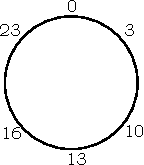
\includegraphics{images/illustrations/modular.pdf}
\end{center}

Om een gegeven getal modulo 26 te herleiden, kunnen we de volgende functie gebruiken:

\[
 f(x) = x - \left\lfloor{\frac{x}{26}}\right\rfloor \times 26
\]

Hieruit blijkt dat we, om de waarde van een getal $x$ modulo 26 te verkrijgen, eerst $x$ door 26 delen en naar beneden afronden, waarmee we het aantal keren bepalen dat we de cirkel rond zijn gegaan. Daarna vermenigvuldigen we dit resultaat weer met 26 en trekken we het van $x$ af. Het eindresultaat is de rest die overblijft en zal altijd een waarde tussen 0 en 25 zijn.

Als voorbeeld is het getal 28 in modulo 26 gelijk aan 2:
\[
	f(28) = 28 - \left\lfloor{\frac{28}{26}}\right\rfloor \times 26 = 28 - 1 \times 26 = 2
\]

Het programma aan het einde van dit hoofdstuk gebruikt deze formule door op regel 30 een overeenkomstige functie te definiëren:

\begin{screencode}
DEF FN F(X)=X-INT(X/26)*26
\end{screencode}

{\bf ROT13:} Om elke letter uit de klare tekst te versleutelen, schuiven we 13 plaatsen naar voren. De letter A uit de klare tekst wordt zo de letter N uit de cijfertekst, B wordt O, waarbij de laatste letters ``terugspringen'' naar het begin van het alfabet. De letter Z uit de klare tekst wordt daardoor de letter M uit de cijfertekst. Hiermee is de versleuteling beschreven. Het ontsleutelen van de cijfertekst werkt op precies dezelfde manier: we herhalen het proces eenvoudigweg door opnieuw 13 plaatsen naar voren te schuiven, waardoor de cirkel rond is en we weer uitkomen waar we begonnen. Zo wordt de letter N uit de cijfertekst weer de letter A uit de klare tekst.

We kunnen dit visueel zien als een afbeelding in tabelvorm:

\Large
\begin{center}
  \begin{tabular}{|c|c|c|c|c|c|c|c|c|c|c|c|c|c|}
  \hline
    Klare tekst & A & B & C & D & E & F & G & H & I & J & K & L & M \\ \hline	ROT13-cijfertekst & N & O & P & Q & R & S & T & U & V & W & X & Y & Z \\ \hline
  \end{tabular}
\end{center}

\begin{center}
  \begin{tabular}{|c|c|c|c|c|c|c|c|c|c|c|c|c|c|}
  \hline
    Klare tekst & N & O & P & Q & R & S & T & U & V & W & X & Y & Z \\ \hline	ROT13-cijfertekst & A & B & C & D & E & F & G & H & I & J & K & L & M \\ \hline
  \end{tabular}
\end{center}

\normalsize

Om met ROT13 te versleutelen, zoekt u de letter van de klare tekst in de bovenste rij en gaat u omlaag naar de onderste rij om de bijbehorende letter van de cijfertekst te vinden. Om met ROT13 te ontsleutelen, zoekt u de letter van de cijfertekst in de onderste rij en gaat u omhoog naar de bovenste rij om de bijbehorende letter van de klare tekst te vinden.

Beschouwen we het ROT13-cijfer vanuit wiskundig oogpunt, dan zien we dat we voor zowel versleutelen als ontsleutelen eenvoudigweg 13 optellen bij de numerieke waarde van een letter uit de klare tekst of de cijfertekst en deze vervolgens modulo 26 herleiden. Dit levert een nieuw getal tussen 0 en 25 op dat overeenkomt met de versleutelde of ontsleutelde letter. De functie $E_{ROT13}$ is de versleutelingsfunctie. Deze aanvaardt de waarde van een letter $x$ uit de klare tekst als argument en geeft de waarde van de bijbehorende letter uit de cijfertekst als resultaat terug. De functie $D_{ROT13}$ is de ontsleutelingsfunctie. Deze aanvaardt de waarde van een letter $x$ uit de cijfertekst als argument en geeft de waarde van de bijbehorende letter uit de klare tekst als resultaat terug.

\[
  E_{ROT13}(x) = (x + 13) \bmod 26
\]

\[
  D_{ROT13}(x) = (x + 13) \bmod 26
\]

Merk op dat de definities van zowel de versleutelings- als de ontsleutelingsfunctie in dit geval precies hetzelfde zijn.

{\bf Atbasj:} Atbasj is een eeuwenoude techniek om het Hebreeuwse alfabet van 22 letters te versleutelen, maar we kunnen dezelfde logica toepassen om het Nederlandse alfabet van 26 letters te versleutelen. Om een letter met Atbasj te versleutelen, moeten we het Nederlandse alfabet achterstevoren opschrijven. Zo wordt de letter A uit de klare tekst bij het versleutelen de letter Z uit de cijfertekst, B wordt Y, C wordt X enzovoort. Het ontsleutelen van de cijfertekst werkt op dezelfde manier: de letter A uit de cijfertekst wordt de letter Z uit de klare tekst, B wordt Y, C wordt X enzovoort.

We kunnen dit visueel zien als een afbeelding in tabelvorm:

\Large
\begin{center}
  \begin{tabular}{|c|c|c|c|c|c|c|c|c|c|c|c|c|c|}
  \hline
    Klare tekst & A & B & C & D & E & F & G & H & I & J & K & L & M \\ \hline	Atbasj-cijfertekst & Z & Y & X & W & V & U & T & S & R & Q & P & O & N \\ \hline
  \end{tabular}
\end{center}

\begin{center}
  \begin{tabular}{|c|c|c|c|c|c|c|c|c|c|c|c|c|c|}
  \hline
    Klare tekst & N & O & P & Q & R & S & T & U & V & W & X & Y & Z \\ \hline    Atbasj-cijfertekst & M & L & K & J & I & H & G & F & E & D & C & B & A \\ \hline
  \end{tabular}
\end{center}

\normalsize

Om met Atbasj te versleutelen, zoekt u de letter van de klare tekst in de bovenste rij en gaat u omlaag naar de onderste rij om de bijbehorende letter van de cijfertekst te vinden. Om met Atbasj te ontsleutelen, zoekt u de letter van de cijfertekst in de onderste rij en gaat u omhoog naar de bovenste rij om de bijbehorende letter van de klare tekst te vinden.

Beschouwen we het Atbasj-cijfer vanuit wiskundig oogpunt, dan zien we dat we voor zowel versleutelen als ontsleutelen de numerieke waarde van de klare tekst of de cijfertekst met 25 moeten vermenigvuldigen, er daarna 25 bij moeten optellen en het geheel vervolgens modulo 26 moeten herleiden. Dit levert een nieuw getal tussen 0 en 25 op dat overeenkomt met de versleutelde of ontsleutelde letter. De functie $E_{Atbasj}$ is de versleutelingsfunctie. Deze aanvaardt de waarde van een letter $x$ uit de klare tekst als argument en geeft de waarde van de bijbehorende letter uit de cijfertekst als resultaat terug. De functie $D_{Atbasj}$ is de ontsleutelingsfunctie. Deze aanvaardt de waarde van een letter $x$ uit de cijfertekst als argument en geeft de waarde van de bijbehorende letter uit de klare tekst als resultaat terug.

\[
  E_{Atbasj}(x) = (25 \times x + 25) \bmod 26
\]

\[
  D_{Atbasj}(x) = (25 \times x + 25) \bmod 26
\]

Merk op dat de definities van zowel de versleutelingsfunctie als de ontsleutelingsfunctie in dit geval exact hetzelfde zijn.

{\bf Caesar:} Het Caesar-cijfer is eveneens een eeuwenoude techniek om berichten te versleutelen en te ontsleutelen. Om een letter te versleutelen met het Caesar-cijfer, schuiven we drie plaatsen naar voren. De letter A uit de klare tekst wordt zo de letter D in de cijfertekst, B wordt E, C wordt F enzovoort. Het ontsleutelen van de cijfertekst werkt precies andersom. In plaats van drie plaatsen naar voren te schuiven, schuiven we nu drie plaatsen naar achteren. De letter A uit de cijfertekst wordt zo de letter X in de klare tekst, B wordt Y, C wordt Z enzovoort.

We kunnen dit visueel zien als een afbeelding in tabelvorm:

\Large
\begin{center}
  \begin{tabular}{|c|c|c|c|c|c|c|c|c|c|c|c|c|c|}
  \hline
    Klare tekst & A & B & C & D & E & F & G & H & I & J & K & L & M \\ \hline	Caesar-cijfertekst & D & E & F & G & H & I & J & K & L & M & N & O & P \\ \hline
  \end{tabular}
\end{center}

\begin{center}
  \begin{tabular}{|c|c|c|c|c|c|c|c|c|c|c|c|c|c|}
  \hline
    Klare tekst & N & O & P & Q & R & S & T & U & V & W & X & Y & Z \\ \hline    Caesar-cijfertekst & Q & R & S & T & U & V & W & X & Y & Z & A & B & C \\ \hline
  \end{tabular}
\end{center}

\normalsize

Om met het Caesar-cijfer te versleutelen, zoekt u de letter uit de klare tekst in de bovenste rij op en gaat u naar de onderste rij om de bijbehorende letter uit de cijfertekst te vinden. Om met het Caesar-cijfer te ontsleutelen, zoekt u de letter uit de cijfertekst in de onderste rij op en gaat u naar de bovenste rij om de bijbehorende letter uit de klare tekst te vinden.

Bezien we het Caesar-cijfer vanuit wiskundig oogpunt, dan zien we dat we om te versleutelen 3 moeten optellen bij de numerieke waarde van de letter uit de klare tekst en het resultaat vervolgens modulo 26 moeten reduceren. Dit levert een nieuw getal tussen 0 en 25 op, dat overeenkomt met de versleutelde letter. Om te ontsleutelen, moeten wij 3 van de numerieke waarde van de letter uit de cijfertekst aftrekken en het resultaat modulo 26 reduceren. Dit levert een nieuw getal tussen 0 en 25 op, dat overeenkomt met de ontsleutelde letter.

De functie $E_{Caesar}$ is de versleutelingsfunctie. Zij aanvaardt als argument de waarde $x$ van een letter uit de klare tekst en geeft de waarde van de bijbehorende letter uit de cijfertekst als resultaat terug. De functie $D_{Caesar}$ is de ontsleutelingsfunctie. Zij aanvaardt als argument de waarde $x$ van een letter uit de cijfertekst en geeft de waarde van de bijbehorende letter uit de klare tekst als resultaat terug.

\[
  E_{Caesar}(x) = (x + 3) \bmod 26
\]

\[
  D_{Caesar}(x) = (x - 3) \bmod 26
\]

Merk op dat de definities van zowel de versleutelingsfunctie als de ontsleutelingsfunctie in dit geval verschillend zijn.

Alle drie de bovenstaande methoden kunnen we generaliseren door te stellen dat zij de volgende versleutelings- en ontsleutelingsfuncties gebruiken:

\[
 E(x) = (A_{1}x + B_{1}) \bmod 26
\]

\[
 D(x) = (A_{2}x + B_{2}) \bmod 26
\]

Hierbij zijn $A_{1}$, $A_{2}$, $B_{1}$ en $B_{2}$ constanten, die tezamen de {\it versleutelingssleutel} vormen van een affien cijfer.

Het uitvoeren van het volgende programma toont een tekstmenu. De gebruiker kan kiezen om een tekenreeks te versleutelen of te ontsleutelen, of om het programma af te sluiten. U kunt hiermee oefenen door een zin in klare tekst in te typen, deze te versleutelen en daarna de versleutelde zin weer te ontsleutelen, zodat de oorspronkelijke klare tekst terugkomt.

Een goede voorbeeldtekenreeks om een cijfer mee te testen is:

\texttt{\bf OP BRUTE WIJZE VING DE SCHOOLJUF DE QUASI-KALME LYNX}

Deze tekenreeks is 52 tekens lang en bevat acht spaties, één koppelteken en 43 letters. Elke letter van het alfabet komt ten minste één keer in deze tekenreeks voor, zodat versleutelen en ontsleutelen hiermee controleert dat elke letter op de verwachte wijze wordt omgezet.

Versleuteling van de bovenstaande tekenreeks met het ROT13-cijfer levert het volgende op:

\texttt{\bf BC OEHGR JVWMR IVAT QR FPUBBYWHS QR DHNFV-XNYZR YLAK}

Versleuteling van de bovenstaande tekenreeks met het Atbasj-cijfer levert het volgende op:

\texttt{\bf LK YIFGV DRQAV ERMT WV HXSLLOQFU WV JFZHR-PZONV OBMC}

Versleuteling van de bovenstaande tekenreeks met het Caesar-cijfer levert het volgende op:

\texttt{\bf RS EUXWH ZLMCH YLQJ GH VFKRROMXI GH TXDVL-NDOPH OBQA}

\begin{screencode}
10 REM *** CRYPTOGRAFIE ***
20 POKE 0,65: PRINT CHR$(142): PRINT CHR$(147)
30 DEF FN F(X)=X-INT(X/26)*26
40 C$="": P$=""
50 PRINT "SELECT AN OPTION (E, D OR Q):": PRINT
60 PRINT "{SPACE*3}[V] KLARE TEKST VERCIJFEREN": PRINT
70 PRINT "{SPACE*3}[O] CIJFERTEKST ONTCIJFEREN": PRINT
80 PRINT "{SPACE*3}[E] EINDE": PRINT
90 GET S$
100 IF (S$="E") THEN END
110 IF (S$="V") THEN GOSUB 150: GOTO 40
120 IF (S$="O") THEN GOSUB 270: GOTO 40
130 GOTO 90
140 REM VERCIJFEREN
150 INPUT "VOER DE BOODSCHAP IN KLARE TEKST IN: ", P$
160 IF P$="" THEN GOTO 150
170 M$=P$: GOSUB 390
180 IF (V=0) THEN GOSUB 460: GOTO 150
190 A=1:B=3
200 FOR I=1 TO LEN(P$)
210 :   L$ = MID$(P$,I,1)
220 :   IF (L$=" ") THEN C$=C$+" ": ELSE C$=C$+CHR$(65+(FN F(A*(ASC(L$)-65)+B)))
230 NEXT I
240 PRINT: PRINT "{REVERSE ON}DE CIJFERTEKST IS:{REVERSE OFF}", C$: PRINT
250 RETURN
260 REM ONTCIJFEREN
270 INPUT "VOER DE VERCIJFERDE BOODSCHAP IN: ", C$
280 IF C$="" THEN GOTO 270
290 M$=C$: GOSUB 390
300 IF (V=0) THEN GOSUB 460: GOTO 270
310 A=1: B=-3
320 FOR I=1 TO LEN(C$)
330 :   L$ = MID$(C$,I,1)
340 :   IF (L$=" ") THEN P$=P$+" ": ELSE P$=P$+CHR$(65+(FN F(A*(ASC(L$)-65)+B)))
350 NEXT I
360 PRINT: PRINT "{REVERSE ON}ONTCIJFERDE KLARE TEKST:{REVERSE OFF}", P$: PRINT
370 RETURN
380 REM VALIDATE
390 V = 1
400 FOR I=1 TO LEN(M$)
410 :   L$ = MID$(M$,I,1)
420 :   IF NOT (((L$ >= "A") AND (L$ <= "Z")) OR (L$=" ")) THEN V = 0
430 NEXT I
440 RETURN
450 REM FOUTMELDING
460 PRINT: PRINT "GEBRUIK UITSLUITEND LETTERS EN SPATIES": PRINT
470 RETURN
\end{screencode}

Indien u het ROT13-cijfer wilt gebruiken, moet u de volgende regels wijzigen:
\begin{screencode}
190 A=1: B=13
310 A=1: B=13
\end{screencode}

Indien u het Atbasj-cijfer wilt gebruiken, moet u de volgende regels wijzigen:
\begin{screencode}
190 A=25: B=25
310 A=25: B=25
\end{screencode}

Indien u het Caesar-cijfer wilt gebruiken, moet u de volgende regels wijzigen:
\begin{screencode}
190 A=1: B=3
310 A=1: B=-3
\end{screencode}

De programmalijst, zoals die nu staat, gebruikt standaard het Caesar-cijfer.

\input{dutch/morebasic}
\input{dutch/datainbasic}
\chapter {C64-, C65- en MEGA65-modi}
\label{cha:modes}

De MEGA65 heeft, net als de C65 en de C128, meerdere bedrijfsmodi. Tussen de MEGA65 en beide eerdere computers bestaan evenwel belangrijke verschillen.

Standaard start het bestand {\tt MEGA65.ROM} op in de MEGA65-modus (waaronder BASIC 65) en biedt het een methode om via het \screentext{GO 64}-commando naar de C64-modus te schakelen. Het is evenwel ook mogelijk om een originele C65-ROM (versie {\tt 91XXXX.BIN}) die naar {\tt MEGA65.ROM} is hernoemd te gebruiken, waardoor de MEGA65 in de C65-modus met BASIC 10 opstart. Ook deze ROM biedt dezelfde functionaliteit om naar de C64-modus te schakelen.

Afhankelijk van uw keuze voor de opstart-ROM hebt u derhalve:

\begin{center}
\begin{tabular}{|l|l|l|l|}
 \hline
  {\textbf{Opstartmodus}} & {\textbf{ROM-versie}} & {\textbf{BASIC}} & {\textbf{C64-modus}} \\
 \hline
   MEGA65    & \screentext{92XXXX}      & BASIC 65 & \screentext{GO 64} \\   C65       & \screentext{91XXXX}      & BASIC 10 & \screentext{GO 64} \\
 \hline
\end{tabular}
\end{center}
Voor lezers die bekend zijn met de C128 is het belangrijkste verschil dat alle nieuwe voorzieningen van de MEGA65 vanuit elke modus toegankelijk zijn en dat u zelfs tussen de verschillende modi heen en weer kunt schakelen. Het is ook mogelijk om hybride modi te maken die voorzieningen uit de verschillende modi combineren -- alles wat u nodig hebt, is de {\bf MAP}-instructie en het adres van het KEY-register, namelijk {\bf 53295} (\$D02F).

Dit hoofdstuk behandelt de verschillende modi, de {\bf MAP}-instructie en het KEY-register. Met het KEY-register kunt u de bedrijfsmodus van de MEGA65 wijzigen. Daarnaast legt dit hoofdstuk uit hoe u met BASIC-commando's van de ene modus naar de andere schakelt.

\phantomsection
\section{Modi wisselen vanuit BASIC}

De MEGA65 werkt in de C64-modus (met BASIC 2), in de C65-modus (met BASIC 10) bij ROM-versies {\tt 91XXXX}, of in de MEGA65-modus (met BASIC 65) bij ROM-versies {\tt 92XXXX}.

Verschillende MEGA65-voorzieningen kunt u echter vanuit alle modi benaderen en alle MEGA65-voorzieningen staan ter beschikking van programma's die in assembleertaal / machinetaal zijn geschreven.
\ifdefined\printmanual
Voor meer informatie over het schrijven van zulke programma's raadpleegt u het {\bf grote Mega65-boek}.
\else
Meer informatie over het schrijven van zulke programma's vindt u in de verschillende bijlagen.
\fi

\subsection{Van MEGA65/C65 naar de C64-modus}

Om van MEGA65/C65 naar de C64-modus te schakelen, gebruikt u het vertrouwde \screentext{GO 64}-commando dat identiek is aan het overschakelen naar de C64-modus op een C128:
\index{BASIC 65-voorbeelden!GO64}
\begin{tcolorbox}[colback=black,coltext=white]
\verbatimfont{\codefont}
\begin{verbatim}
GO 64
ARE YOU SURE? Y
\end{verbatim}
\end{tcolorbox}

Let op dat alle programma's in het geheugen verloren gaan bij het wisselen van modus. Dit is hetzelfde als bij de C128.
\index{Toetsenbord!MEGA-toets}
U kunt ook \megasymbolkey ingedrukt houden terwijl u op de resetknop drukt of de MEGA65 inschakelt. Ook dit is hetzelfde als bij de C128.

\subsection{Van C64 naar de MEGA65/C65-modus}

Om van C64 naar de MEGA65/C65-modus te schakelen, gebruikt u het volgende commando. {\bf Let op: dit commando vraagt niet om bevestiging}!

\begin{tcolorbox}[colback=black,coltext=white]
\verbatimfont{\codefont}
\begin{verbatim}
SYS 58552
\end{verbatim}
\end{tcolorbox}

U kunt ook terugkeren naar de MEGA65/C65-modus door op de resetknop aan de linkerkant van de MEGA65 te drukken of door de MEGA65 uit en weer in te schakelen.

Een andere mogelijkheid is om \widekey{RESTORE} een halve tot één seconde ingedrukt te houden en vervolgens in het Freezer-menu op \megakey {F5} te drukken. Dit simuleert het indrukken van de resetknop.

Let op dat alle programma's in het geheugen verloren gaan bij het wisselen van modus. Dit is hetzelfde als bij de C128.

\subsection{De machinetaalmonitormodus openen}

De machinetaalmonitor opent u door vanuit BASIC 65/10 het commando {\bf MONITOR} in te typen, of door \specialkey{RUN\\STOP} ingedrukt te houden en vervolgens op de resetknop aan de linkerkant van de MEGA65 te drukken.

\phantomsection
\section{Het KEY-register}

De MEGA65 heeft een VIC-IV als videocontroller in plaats van de VIC-II van de C64 of de VIC-III van de C65. Net zoals de VIC-III extra registers heeft ten opzichte van de VIC-II, heeft de VIC-IV er nog meer. Als deze registers voortdurend zichtbaar zouden zijn, bestaat de kans dat software die voor de C64 en de VIC-II is gemaakt, onbedoeld gebruikmaakt van deze nieuwe registers, wat tot onverwacht gedrag leidt. De makers van de C65 hebben derhalve een manier bedacht om de extra registers van de VIC-III voor oude C64-programma's te verbergen. Het in- en uitschakelen (of verbergen en weer zichtbaar maken) van de extra registers gebeurt via het KEY-register. Voor meer informatie over welke registers in elk van de I/O-modi van de VIC-II, VIC-III en VIC-IV zijn uit- en ingeschakeld, raadpleegt u
\ifdefined\printmanual
 het {\bf grote Mega65-boek}.
\else
 \bookvref{sec:iopersonalities}.
\fi

% iopersonalities results in ?? (??) when building on my machine

Het KEY-register, dat zich op adres {\bf 53295} bevindt, is een ongebruikt register van de VIC-II, waarin u met {\bf POKE} kunt schrijven en waaruit u met {\bf PEEK} kunt lezen, net als bij andere registers. Het KEY-register heeft echter een bijzondere functie: schrijft u er twee bepaalde waarden vlak na elkaar naar toe, dan kunt u de VIC-IV opdracht geven om de registers van de VIC-III of VIC-IV niet langer voor de rest van de MEGA65 verborgen te houden.

\subsection{Extra C65-registers zichtbaar maken}

Om bijvoorbeeld de nieuwe registers van de VIC-III in de C64-modus in te schakelen, moet u de waarden 165 en 150 met {\bf POKE} in het KEY-register schrijven. De eenvoudigste manier hiervoor is om de MEGA65 uit en weer in te schakelen, GO 64 te typen en met Y te antwoorden om in de C64-modus te komen.

\underline{OPMERKING}: Voert u deze POKE's uit terwijl de MEGA65 zich in de C65-modus bevindt, dan kan het voorkomen dat de MEGA65 niet correct functioneert.

Bent u eenmaal in de C64-modus, probeer dan de volgende commando's in te typen:
\index{BASIC 65-voorbeelden!POKE}
\begin{tcolorbox}[colback=black,coltext=white]
\verbatimfont{\codefont}
\begin{verbatim}
POKE 53295,165: POKE 53295,150
\end{verbatim}
\end{tcolorbox}

Zodra u deze commando's intypt, geeft de MEGA65 de \screentextwide{READY.}-prompt terug en lijkt er verder niets te gebeuren. Dat is te verwachten, want de MEGA65 heeft slechts de nieuwe registers van de VIC-III ingeschakeld (en enkele andere functies uit de C65-modus). De C64-BASIC en de KERNAL blijven normaal functioneren en het lijkt wel of er niets is veranderd... Er \textit{is} echter wel degelijk iets veranderd.

Zo kunt u bijvoorbeeld iets doen wat de C64 met zijn VIC-II niet kan: de ene kleur geleidelijk in de andere laten overgaan. De VIC-III heeft registers waarmee u de rood-, groen- en blauwcomponenten van de kleuren kunt wijzigen. Nu de registers van de VIC-III zijn ingeschakeld, kunt u de kleur van de achtergrond geleidelijk van blauw naar paars laten overgaan, door de roodcomponent van de kleur die op de C64 normaal blauw is te vergroten. De registers voor de waarde van de roodcomponent liggen op 53504 -- 53759 (\$D100 -- \$D1FF). Blauw is kleur 6, dus u moet register 53510 (53504 + 6, of \$D106) wijzigen. Een voorbeeldlisting in BASIC met een {\bf FOR}-lus om de kleur te wijzigen is:

\begin{tcolorbox}[colback=black,coltext=white]
\verbatimfont{\codefont}
\begin{verbatim}
FOR I = 0 TO 15 STEP 0.2 : POKE 53510,I : NEXT
\end{verbatim}
\end{tcolorbox}

Eenmaal het programma is ingetypd, typt u {\bf RUN} op een nieuwe regel. De achtergrond van het scherm vervaagt daarna van blauw naar paars. Wilt u het effect sneller laten verlopen, vergroot dan de 0.2 naar een groter getal, zoals 0.5. Langzamer gaat het met een kleiner getal, zoals 0.02. U kunt de roodcomponent ook wijzigen door met {\bf POKE} een ander getal naar 53504 – 53759 (\$D100 – \$D1FF) te schrijven, de groencomponent op 53760 -- 54015 (\$D200 -- \$D2FF), of de blauwcomponent op 54016 -- 54271 (\$D300 -- \$D3FF). Om bijvoorbeeld de rand en de tekst (beide zijn normaal ``lichtblauw'') van blauw naar groen te laten overgaan, kunt u het volgende proberen:

\begin{tcolorbox}[colback=black,coltext=white]
\verbatimfont{\codefont}
\begin{verbatim}
POKE 53518,0 : FOR I = 0 TO 15 STEP 0.1 : POKE 53774,I : POKE 54030,15-I : NEXT
\end{verbatim}
\end{tcolorbox}

\subsection{Extra C65/MEGA65-registers uitschakelen}

U kunt de registers van de VIC-III ook weer uitschakelen door met {\bf POKE} een willekeurig getal in het KEY-register te schrijven, bijv.:

\begin{tcolorbox}[colback=black,coltext=white]
\verbatimfont{\codefont}
\begin{verbatim}
POKE 53295,0
\end{verbatim}
\end{tcolorbox}

Voert u de bovenstaande voorbeelden opnieuw uit met {\bf RUN}, dan veranderen de kleuren niet, omdat de registers zijn uitgeschakeld. In plaats daarvan verandert het schrijven naar die adressen enkele registers van de VIC-II, omdat deze op een C64 meerdere keren voorkomen. Voor het bovenstaande voorbeeld valt dat gelukkig mee: de gebruikte registers hebben geen voor de hand liggende neveneffecten. Dat komt doordat de registers die in de voorbeelden hierboven worden gewijzigd, op een standaard VIC-II worden gebruikt om de spriteposities te wijzigen. Omdat er geen sprites op het scherm staan, ziet u niets veranderen.

\subsection{Extra MEGA65-registers inschakelen}

De MEGA65 heeft \textit{nog meer} registers dan de C65. Om deze in de C64-modus in te schakelen, moet u nog twee waarden met {\bf POKE} in het KEY-register schrijven:

\begin{tcolorbox}[colback=black,coltext=white]
\verbatimfont{\codefont}
\begin{verbatim}
POKE 53295,71: POKE 53295,83
\end{verbatim}
\end{tcolorbox}

Ook nu merkt u niet onmiddellijk een verschil, net als bij het inschakelen van de registers van de VIC-III. De MEGA65 kan er nu echter niet alleen de registers van de VIC-II en VIC-III mee aanspreken, maar ook die van de VIC-IV. Wilt u dat zelf controleren, dan kunt u de voorbeelden van eerder in dit hoofdstuk proberen en ziet u dat de registers van de VIC-III weer toegankelijk zijn. Bovendien kunt u er nu ook dingen mee doen die specifiek zijn voor de MEGA65. Wilt u bijvoorbeeld het begin van de bovenrand hoger op het scherm laten beginnen, dan kunt u zoiets als het volgende proberen:

\begin{tcolorbox}[colback=black,coltext=white]
\verbatimfont{\codefont}
\begin{verbatim}
POKE 53320,60
\end{verbatim}
\end{tcolorbox}

U kunt ook voor de aardigheid de schermranden animeren, door ze dichter bij elkaar en verder uit elkaar te laten bewegen:

\begin{tcolorbox}[colback=black,coltext=white]
\verbatimfont{\codefont}
\begin{verbatim}
FOR I = 255 TO 0 STEP -1 : POKE 53320,I : POKE 53322, 255 - I : NEXT
\end{verbatim}
\end{tcolorbox}

Het bovenstaande voorbeeld laat de lus achteruit tellen (van 255 naar 0), zodat u niet met slechts een piepklein strookje zichtbare tekst komt te zitten. U kunt de lus desgewenst ook vooruit laten tellen. Blijft u steken met slechts een strookje van het scherm, dan kunt u \specialkey{RUN\\STOP} en \widekey{RESTORE} indrukken. U vraagt zich wellicht af: waarom werken \specialkey{RUN\\STOP} en \widekey{RESTORE}, terwijl het hier registers van de VIC-IV betreft die de BASIC en de KERNAL in de C64-modus niet kennen? De verklaring is dat de VIC-IV een functie heeft die ``hete registers'' heet, waarbij bepaalde registers van de C64 en C65 ertoe leiden dat sommige registers van de MEGA65 naar de standaardwaarden van de C64- of C65-modus worden teruggezet. In dit specifieke geval is het de KERNAL die het VIC-II-scherm opnieuw instelt via 53265 (\$D011); dit register stelt in de C64/C65-modus de grootte van de verticale rand bij en is dus een ``heet register'' voor de registers met de verticale randpositie van de MEGA65.

Kijk of u het scherm in plaats daarvan kunt laten schudden door de registers TEXTXPOS en TEXTYPOS van de VIC-IV te wijzigen. De {\bf POKE}-codes voor die registers, en voor nog veel meer andere interessante nieuwe registers, vindt u door te bladeren in
\ifdefined\printmanual
 het {\bf grote Mega65-boek}.
\else
 \bookvref{cha:viciv}.
\fi


\subsection{Valkuilen}

In alle modi zet de DOS van het interne 3.5''-diskettestation (ook wanneer u D81-schijfimages van een SD-kaart gebruikt) het KEY-register bij elke toegang terug naar de VIC-II-modus. Voert u derhalve acties uit zoals het opvragen van de stationstatus, of het laden of opslaan van een bestand met {\bf LOAD} of {\bf SAVE}, dan wordt het KEY-register gereset en worden uitsluitend de registers van de VIC-II ingeschakeld. U kunt de registers van de C65 of de MEGA65 uiteraard weer inschakelen door de juiste waarden opnieuw met {\bf POKE} naar het KEY-register te schrijven.

\phantomsection
\section{Geheugen benaderen vanuit BASIC 65}

BASIC 65 bevat krachtige commando's voor geheugenbanking en Direct Memory Access (DMA), waarmee u geheugengebieden buiten de 128KB RAM van de C65 kunt lezen, vullen, kopiëren en beschrijven. De MEGA65 heeft 384KB hoofdgeheugen, verdeeld over 6 banken van elk 64KB. Dat zijn:
\begin{itemize}
 \item BANK 0 en BANK 1 - vormen samen de normale 128KB RAM van de C65. \item BANK 2 en BANK 3 - zijn doorgaans schrijfbeveiligd en bevatten het ROM-image van de C65. \item BANK 4 en BANK 5 - worden gebruikt voor alle grafische routines van BASIC 65 voor bitplanegrafiek met hoge resolutie.       BASIC 10 gebruikt de banken 4 en 5 niet.
\end{itemize}
\index{BASIC 65-voorbeelden!BANK}
\index{BASIC 65-voorbeelden!PEEK}
\index{BASIC 65-voorbeelden!POKE}
Met de commando's {\bf BANK}, {\bf PEEK} en {\bf POKE} kunt u dit geheugengebied eenvoudig benaderen, bijvoorbeeld:

\begin{tcolorbox}[colback=black,coltext=white]
\verbatimfont{\codefont}
\begin{verbatim}
BANK 4: POKE0,123: REM PLAATS 123 IN LOCATIE $40000
BANK 4: PRINT PEEK(0): REM TOON INHOUD VAN LOCATIE $40000
\end{verbatim}
\end{tcolorbox}

U kunt de huidige inhoud van het scherm en het kleurengeheugen (colour-RAM) echter ook met het {\bf DMA}-commando naar BANK 4 kopiëren:
\index{BASIC 65-voorbeelden!DMA}
\begin{tcolorbox}[colback=black,coltext=white]
\verbatimfont{\codefont}
\begin{verbatim}
DMA 0, 2000, 2048, 0, 0, 4 : REM SCHERMTEKST NAAR BANK 4
DMA 0, 2000, DEC("F800"), 1, 2000, 4 : REM KOPIEER KLEURENRAM NAAR BANK 4
\end{verbatim}
\end{tcolorbox}

Vervolgens kunt u iets anders op het scherm zetten en dit met het volgende commando terugkopiëren:

\begin{tcolorbox}[colback=black,coltext=white]
\verbatimfont{\codefont}
\begin{verbatim}
DMA 0, 2000, 0, 4, 2048, 0 : REM SCHERMTEKST VANUIT BANK 4
DMA 0, 2000, 2000, 4, DEC("F800"), 1 : REM KOPIEER KLEURENRAM VANUIT BANK 4
\end{verbatim}
\end{tcolorbox}

\index{BASIC 65-voorbeelden!MAP}
\phantomsection
\section{De MAP-instructie}

De bovenstaande methoden kunt u vanuit BASIC gebruiken. De {\bf MAP}-instructie is daarentegen een assembleertaalinstructie, waarmee u het geheugen van de MEGA65 opnieuw kunt indelen. De C65-ROM en BASIC 65 gebruiken deze instructie om te beheren welk geheugen op elk gegeven moment bruikbaar is. Voor een nadere toelichting op de {\bf MAP}-instructie verwijzen wij u naar de betreffende sectie van
\ifdefined\printmanual
 het {\bf grote Mega65-boek}.
\else
 \bookvref{sec:map-instruction}.
\fi





\part{GELUID EN GRAFIEK}


\newcommand{\blkb}{\cellcolor[rgb]{0,0,0}\textcolor{white} 0 }
\newcommand{\bwn}{\cellcolor[rgb]{.26,.22,0}\textcolor{white} 9 }
\newcommand{\ora}{\cellcolor[rgb]{.44,.31,.15}8 }
\newcommand{\red}{\cellcolor[rgb]{.6,.4,.35}A }
\newcommand{\lgr}{\cellcolor[rgb]{.58,.58,.58}F }
\newcommand{\yel}{\cellcolor[rgb]{1.,.95,0.}7 }

\newcommand{\redb}{\cellcolor[rgb]{.6,.4,.35} 1 }

\chapter{Grafiek}
\label{cha:graphics}

Laten we nu eens plezier beleven aan grafiek! In dit deel van het boek willen wij de grafiekmodi van de MEGA65 bekijken door voorbeeldcode in machinetaal en BASIC stap voor stap te doorlopen, zodat u de verschillende mogelijkheden van de MEGA65 op het gebied van grafiek leert kennen. Allereerst is het belangrijk te weten dat de MEGA65 drie verschillende basisgrafiekmodi ondersteunt:

\begin{itemize}
	\item Bitmapgrafiek	\item Grafiek gebaseerd op tekensets	\item Bitplanes
\end{itemize}


\section*{Bitmapgrafiek}

In bitmapgrafiek wordt elke pixel van een afbeelding afzonderlijk opgeslagen. De manier waarop de pixels in het geheugen worden bewaard, verschilt van systeem tot systeem en hangt in de meeste gevallen af van de prestaties van de hardware. Als het geheugen onbeperkt zou zijn, zou de eenvoudigste manier om een pixel te onthouden zijn om zijn RGB-waarden in drie aparte bytes op te slaan. Voorbeeld: 0xFFFFFF voor wit zou betekenen dat er drie waarden opgeslagen moeten worden: \$FF, \$FF en \$FF. Eerlijk gezegd is dit te eenvoudig en niet echt efficiënt. Laten wij dus een andere manier bedenken. Waarom leggen wij niet een kleurentabel (of kleurenpalet) vast, slaan de RGB-waarden één keer op en verwijzen daarna alleen nog naar de kleur via de index ervan in de tabel? Dat bespaart ons veel geheugen! Stel dat wij een kleurrijke 8x8-bitmap maken, die op het scherm een ``A'' moet voorstellen. Kleurrijk wil hier zeggen dat wij hem in wat bruintinten willen hebben. De kleurentabel daarvoor kan er dan als volgt uitzien:

\begin{center}
\begin{tabular}{|l|l|}
\hline
	Index & Kleur \\
\hline
	\blkb & Zwart \\	\bwn & Bruin \\	\ora & Oranje \\	\red & Lichtrood \\	\lgr & Lichtgrijs \\	\yel & Geel \\
\hline
\end{tabular}
\end{center}

De kleurwaarden zijn overigens precies dezelfde als de kleurwaarden uit het standaard C64-kleurenpalet. Daarna ontwerpen we de ``A''. Elke pixel verwijst naar een waarde uit de bovenstaande kleurentabel.


\begin{center}
\begin{tabular}{|m{6pt}|m{6pt}m{6pt}m{6pt}m{6pt}m{6pt}m{5pt}m{6pt}m{6pt}|}
\hline
	& 7 & 6 & 5 & 4 & 3 & 2 & 1 & 0 \\
\hline
	0 & \blkb & \blkb & \blkb & \blkb & \blkb & \blkb & \blkb & \blkb \\	1 & \red & \lgr & \yel & \lgr & \red & \ora & \blkb & \blkb \\	2 & \lgr & \lgr & \blkb & \blkb & \ora & \red & \blkb & \blkb \\	3 & \yel & \yel & \blkb & \blkb & \ora & \red & \blkb & \blkb \\	4 & \yel & \lgr & \lgr & \red & \red & \red & \blkb & \blkb \\	5 & \lgr & \red & \blkb & \blkb & \ora & \red & \blkb & \blkb \\	6 & \red & \red & \blkb & \blkb & \red & \red & \blkb & \blkb \\	7 & \ora & \bwn & \blkb & \blkb & \ora & \red & \blkb & \blkb \\
\hline
\end{tabular}
\end{center}

Hoeveel geheugen gebruikt dit kleine afbeeldingetje eigenlijk?

Als we een eendimensionale array maken, krijgen we een array met 64 elementen, want onze afbeelding bestaat uit 8x8 pixels = 64 kleurwaarden die opgeslagen moeten worden. Vertaald naar het geheugen van de MEGA65 betekent dit dat we 64 bytes in het geheugen moeten bewaren. Een afbeelding die het volledige scherm vult, bestaat evenwel uit veel meer pixels. Op de C64 en natuurlijk ook op de MEGA65 zijn 320x200 pixels nodig om een afbeelding te maken die het hele scherm vult. Als we dat naar onze array doorrekenen, komen we uit op in totaal 64000 elementen. Omgerekend naar het geheugen van de MEGA65 zijn dat 64000 bytes, oftewel bijna 64 kilobyte aan gegevens! Als we daarbij ook nog bedenken dat de goede oude C64 slechts over 64K RAM beschikte, dan wordt de dramatiek duidelijk! Dat is simpelweg veel te veel gegevens! We hebben strategieën nodig om onze bitmapgegevens te beperken. Op de C64 waren er twee typen bitmapgrafieken, elk met zijn eigen mechanismen om het geheugengebruik tot een minimum te beperken.

\begin{itemize}
	\item Hires	\item Multicolour (MCM)
\end{itemize}


\subsection*{Hires}

Allereerst delen we een bitmap op in blokken van elk 8x8 pixels. Om de volledige resolutie van 320x200 pixels te bereiken, vormen 40 van zulke blokken naast elkaar één regel. Bouwen we vervolgens 25 van die regels op, dan komen we uit op een afbeelding die het volledige scherm vult.

\begin{adjustbox}{width=\textwidth,center}
\begin{footnotesize}
\begin{tabular}[h]{|C{10pt}|C{5pt}|C{5pt}|C{5pt}|C{5pt}|C{5pt}|C{5pt}|C{5pt}|C{5pt}|C{5pt}|C{5pt}|C{5pt}|C{5pt}|C{5pt}|C{5pt}|C{5pt}|C{5pt}|C{5pt}|C{5pt}|C{5pt}|C{5pt}|C{5pt}|C{5pt}|C{5pt}|C{5pt}|C{5pt}|C{5pt}|C{5pt}|C{5pt}|C{5pt}|C{5pt}|C{5pt}|C{5pt}|C{5pt}|C{5pt}|C{5pt}|C{5pt}|C{5pt}|C{5pt}|C{5pt}|C{5pt}|}
\hline
  &   &   &  &  &  &   &   &   &   & 1  & 1  & 1  & 1  & 1  & 1  & 1  & 1  & 1  & 1  & 2  & 2  & 2  & 2  & 2  & 2  & 2  & 2  & 2  & 2  & 3  & 3  & 3  & 3  & 3  & 3  & 3  & 3  & 3  & 3  & 4  \\  & 1 & 2 & 3& 4& 5& 6 & 7 & 8 & 9 &  0 & 1  &  2 &  3 &  4 &  5 &  6 &  7 &  8 &  9 &  0 &  1 &  2 &  3 &  4 &  5 &  6 &  7 &  8 &  9 &  0 &  1 &  2 &  3 &  4 &  5 &  6 &  7 &  8 &  9 &  0 \\
\hline
   1 & & & & & & & & & & & & & & & & & & & & & & & & & & & & & & & & & & & & & & & & \\\hline   2 & & & & & & & & & & & & & & & & & & & & & & & & & & & & & & & & & & & & & & & & \\\hline   3 & & & & & & & & & & & & & & & & & & & & & & & & & & & & & & & & & & & & & & & & \\\hline   4 & & & & & & & & & & & & & & & & & & & & & & & & & & & & & & & & & & & & & & & & \\\hline   5 & & & & & & & & & & & & & & & & & & & & & & & & & & & & & & & & & & & & & & & & \\\hline   6 & & & & & & & & & & & & & & & & & & & & & & & & & & & & & & & & & & & & & & & & \\\hline   7 & & & & & & & & & & & & & & & & & & & & & & & & & & & & & & & & & & & & & & & & \\\hline   8 & & & & & & & & & & & & & & & & & & & & & & & & & & & & & & & & & & & & & & & & \\\hline   9 & & & & & & & & & & & & & & & & & & & & & & & & & & & & & & & & & & & & & & & & \\\hline  10 & & & & & & & & & & & & & & & & & & & & & & & & & & & & & & & & & & & & & & & & \\\hline  11 & & & & & & & & & & & & & & & & & & & & & & & & & & & & & & & & & & & & & & & & \\\hline  12 & & & & & & & & & & & & & & & & & & & & & & & & & & & & & & & & & & & & & & & & \\\hline  13 & & & & & & & & & & & & & & & & & & & & & & & & & & & & & & & & & & & & & & & & \\\hline  14 & & & & & & & & & & & & & & & & & & & & & & & & & & & & & & & & & & & & & & & & \\\hline  15 & & & & & & & & & & & & & & & & & & & & & & & & & & & & & & & & & & & & & & & & \\\hline  16 & & & & & & & & & & & & & & & & & & & & & & & & & & & & & & & & & & & & & & & & \\\hline  17 & & & & & & & & & & & & & & & & & & & & & & & & & & & & & & & & & & & & & & & & \\\hline  18 & & & & & & & & & & & & & & & & & & & & & & & & & & & & & & & & & & & & & & & & \\\hline  19 & & & & & & & & & & & & & & & & & & & & & & & & & & & & & & & & & & & & & & & & \\\hline  20 & & & & & & & & & & & & & & & & & & & & & & & & & & & & & & & & & & & & & & & & \\\hline  21 & & & & & & & & & & & & & & & & & & & & & & & & & & & & & & & & & & & & & & & & \\\hline  22 & & & & & & & & & & & & & & & & & & & & & & & & & & & & & & & & & & & & & & & & \\\hline  23 & & & & & & & & & & & & & & & & & & & & & & & & & & & & & & & & & & & & & & & & \\\hline  24 & & & & & & & & & & & & & & & & & & & & & & & & & & & & & & & & & & & & & & & & \\\hline  25 & & & & & & & & & & & & & & & & & & & & & & & & & & & & & & & & & & & & & & & & \\\hline
\end{tabular}
\end{footnotesize}
\end{adjustbox}

De opdeling in blokken is zinvol, want daardoor kunnen wij de gegevens aanzienlijk verkleinen. Elke regel van een 8x8-blok bestaat uit 8 bits, dus waarom zouden wij de kleurindexen niet loslaten en simpelweg afspreken dat een gezette pixel een ``1'' in de regel voorstelt en een niet-gezette pixel overeenkomt met ``0''.

\begin{center}
\begin{tabular}{|C{12pt}|C{12pt}C{12pt}C{12pt}C{12pt}C{12pt}C{12pt}C{12pt}C{12pt}|R{24pt}|R{24pt}|}
\hline
	& 7 & 6 & 5& 4& 3&  2& 1& 0 & dec & hex \\
\hline
0 & \blkb & \blkb & \blkb & \blkb & \blkb & \blkb & \blkb & \blkb &   0 & 00 \\1 & \blkb & \redb & \redb & \redb & \redb & \blkb & \blkb & \blkb & 120 & 78 \\2 & \redb & \redb & \blkb & \blkb & \redb & \redb & \blkb & \blkb & 204 & CC \\3 & \redb & \redb & \blkb & \blkb & \redb & \redb & \blkb & \blkb & 204 & CC \\4 & \redb & \redb & \redb & \redb & \redb & \redb & \blkb & \blkb & 252 & FC \\5 & \redb & \redb & \blkb & \blkb & \redb & \redb & \blkb & \blkb & 204 & CC \\6 & \redb & \redb & \blkb & \blkb & \redb & \redb & \blkb & \blkb & 204 & CC \\7 & \redb & \redb & \blkb & \blkb & \redb & \redb & \blkb & \blkb & 204 & CC \\
\hline
\end{tabular}
\end{center}

Zoals hierboven te zien is, kunt u de bits van elke regel nu eenvoudig omrekenen naar de bijbehorende hexadecimale waarde en houdt u uiteindelijk 8 bytes aan gegevens over. Dit is de centrale gedachte achter hires-grafiek en met dit concept bespaart u veel geheugen. In dit voorbeeld zijn het 8 bytes, tegenover het vorige voorbeeld, waarin 64 bytes nodig waren om alle kleurverwijzingen te beheren. Rekenen we het eens door voor een afbeelding die het volledige scherm vult: we hebben 40x25 blokken, dat zijn er in totaal 1000. Elk blok is 8 bytes, dus dat levert ``slechts'' 8K op voor een afbeelding op volledig scherm.\\

Dit is een briljante oplossing, maar nu hebben wij een probleem: wij zijn de kleuren kwijt!\\

Als u naar de eerste afbeelding kijkt, ziet u dat die erg kleurrijk was. Hebben we die vele kleuren echter wel nodig? Dit is het tweede belangrijke concept in hires-bitmapgrafiek: minder kleuren betekent minder geheugen. De hires-modus beperkt u in feite tot \textbf{twee kleuren} per 8x8-pixelblok. Deze informatie wordt bewaard in het schermgeheugen (Screen-RAM) en niet, zoals u misschien zou aannemen, in het kleurengeheugen (Colour-RAM). Ook het idee erachter is opnieuw erg vernuftig: in het schermgeheugen kunt u waarden tussen \$00 en \$FF bewaren, terwijl het in het kleurengeheugen alleen zin heeft om waarden tussen \$0 en \$0F op te slaan, om één specifieke kleur uit het C64-kleurenpalet aan te duiden, dat uit 16 kleuren bestaat (\$0-\$F). Op de MEGA65 zijn zelfs nog meer kleuren mogelijk en u kunt de standaardkleuren aanpassen, maar dat wordt later uitgelegd.\\

Terug naar het schermgeheugen. Hier bewaart u \textbf{twee kleuren} voor elk 8x8-blok. Als u de byte splitst in zijn hoge en lage nibble, heeft u de mogelijkheid om er een achtergrond- en een voorgrondkleur in onder te brengen! De hexadecimale waarde \$0a bijvoorbeeld kunt u lezen als \$0 (hoge nibble) en \$a (lage nibble). Op die manier krijgen wij een zwarte achtergrond en lichtrood voor de pixels in het blok. Uiteindelijk betekent dit dat een hires-bitmap voor het volledige scherm niet 8 maar 9 kilobyte gebruikt: 8K voor de ruwe bitmapgegevens, zoals eerder genoemd, en nog eens 1K voor de kleuren in het schermgeheugen.\\

\subsection*{Eenvoudige hires-bitmaps programmeren}

Laten we gaan programmeren! We doen dat eerst in BASIC, voordat we overschakelen naar machinetaal. Om bitmapgrafieken op het scherm te brengen, moeten we de VIC-IV-chip configureren. De VIC moet een paar dingen weten voordat de chip de bitmapgegevens kan vinden en lezen. U moet het volgende doen:

\begin{itemize}
	\item Zorg dat u de VIC-registers heeft geactiveerd die u nodig heeft (denk eraan: de MEGA65 biedt verschillende versies van de VIC-chip)	\item Stel de resolutie in	\item Bepaal een locatie voor de bitmapgegevens	\item En schakel ten slotte de bitmapmodus in
\end{itemize}

Al deze instellingen kunt u in verschillende registers van uw MEGA65 configureren. Een overzicht van de bestaande registers van de grafische chip (dat is uiteraard de VIC) vindt u in \bookvref{cha:viciv}.

Uw MEGA65 bevat één grafische chip, de \textbf{VIC-IV}, die voortbouwt op zijn twee voorgangers en aan die voorgangers nieuwe functies in de vorm van extra registers toevoegt. Deze twee voorgangers zijn de \textbf{VIC-II}, zoals die in de oorspronkelijke Commodore 64 werd gebruikt, en de \textbf{VIC-III}, ook wel ``Bill'' genoemd, zoals die voor de Commodore 65 was gepland.

Het is belangrijk te begrijpen dat deze verschillende VIC-versies op elkaar voortbouwen; beschouw ze als modi die u aan of uit kunt zetten. VIC-III breidt de bestaande registers van de VIC-II uit, terwijl de VIC-IV u alle bestaande registers van VIC-II en VIC-III biedt en daarop voortbouwt door aan eerder ongebruikte registers nieuwe functionaliteit toe te voegen. Dat betekent dat in \bookvref{cha:viciv} niet alleen de registers van de VIC-IV belangrijk zijn om te kennen, maar ook die van VIC-II en VIC-III, afhankelijk van welke VIC-modus u wel of niet heeft geactiveerd. Houd hiermee rekening.

\textbf{Zorg dat u de VIC-registers heeft geactiveerd die u nodig heeft} - wat betekent dat? In grote lijnen gebruikt u het nieuwe register \$D02F hex of 53295 decimaal om tussen de VIC-modi te schakelen (d.w.z. om specifieke registers toe te voegen of te verwijderen). Voor het schakelen gebruikt u een zogeheten klopsequentie, door achtereenvolgens twee specifieke waarden te poken:

\begin{tabular}{|l|l|l|}
	\hline
	VIC & Eerste hex/dec & Tweede hex/dec \\
	\hline
	II  & \$00/0 & \$00/0\\	III & \$A5/165 & \$96/150\\	IV  & \$47/71 & \$53/83\\
	\hline
\end{tabular}

Terzijde: de twee waarden waarmee u de VIC-IV activeert, zijn de ASCII-tekens ``G'' en ``S''. Dat zijn de initialen van de maker van de VIC-IV: universitair hoofddocent Paul Gardner-Stephen. Een leuk paaseitje, nietwaar?

Het is belangrijk te begrijpen dat de computer, wanneer u uw MEGA65 inschakelt, in de C64-modus start en vervolgens zoekt naar een C65-compatibele ROM. Wordt een C64-cartridge gedetecteerd of drukt u de MEGA-toets in, dan blijft het systeem in de C64-modus. In dat geval heeft u alleen de C64-registers tot uw beschikking. Vindt het systeem een C65-ROM, dan activeert het de beschikbare registers. Bij de MEGA65-ROM betekent dit dat u alle VIC-registers (II, III en IV) kunt benaderen. Geeft u het GO64-commando, dan beperkt het systeem u tot de VIC-II-registers - maar denk eraan - door de klopsequentie zoals hierboven beschreven uit te voeren, kunt u die registers weer toevoegen! Het maakt dus niet uit in welke ``modus'' u zich bevindt. Alle mogelijkheden zijn overal beschikbaar. De MEGA65 is werkelijk een flexibele machine!


In dit hoofdstuk gaan we ervan uit dat u in de C65-modus werkt en daarbij de standaard-ROM van de MEGA65 met BASIC65 gebruikt.


De volgende stap is het \textbf{instellen van de resolutie}. Volgens de registers in \bookvref{cha:viciv} kunt u dat doen met \$D031 hex, of 53297 decimaal. Dit register is afkomstig van VIC-III. De C65 beschikt over een beeldscherm met 80 kolommen, de C64 had er slechts 40. Om 80 kolommen te realiseren, moet de grafische chip met hogere resoluties overweg kunnen. Wanneer u de computer inschakelt, werkt u in de 80-kolomsmodus met 25 regels, hetgeen neerkomt op een resolutie van 640x200. Om klassieke bitmaps te tonen, moet u terug naar 320x200 (dat zijn de 40 kolommen en 25 regels, zoals al in de eerdere tabel te zien was). De C64 kon 640x200 niet weergeven, dus had de VIC-II geen register nodig om dat te regelen. De C65 beheerst daarentegen beide, zodat u met \$D031 ertussen kunt schakelen. Manipuleert u het register bitgewijs, dan kunt u nog meer instellen: de resolutie (databit 7, H640), de C65-fastmodus (databit 6, FAST) of het in- en uitschakelen van de nieuwe bitplane-modus als alternatief voor klassieke bitmap- of tekengebaseerde grafiek (databit 4, BPM). Sommige registers zijn wel gepland, maar nooit geïmplementeerd. Bijvoorbeeld een H1280-modus op databit 2, welke de C65 in staat moest stellen op te schalen naar 1280x200 of 1280x400. Zie \bookvref{cha:viciv} voor alle fijne details.

De volgende vraag is: hoe kunnen we specifieke bits in een register aansturen? Schakel uw computer in en typ het volgende commando in

\begin{screencode}
PRINT PEEK($D031)
 224
\end{screencode}

U krijgt dan een decimale waarde terug, zoals 224. De decimale waarde helpt u niet verder: u moet het getal omzetten naar zijn binaire voorstelling.

\begin{tabular}{|l|l|l|l|l|l|l|l|l|}
	\hline
	Bit 7 & Bit 6 & Bit 5 & Bit 4 & Bit 3 & Bit 2 & Bit 1 & Bit 0 & Decimale waarde \\	H640 & FAST & ATTR & BPM & V400 & H1280 & MONO & INT & ~ \\
	\hline
    1 & 1 & 1 & 0 & 0 & 0 & 0 & 0 & 224 \\    0 & 1 & 1 & 0 & 0 & 0 & 0 & 0 & 96 \\
	\hline
\end{tabular}

De eerste rij in de tabel toont het binaire getal voor decimaal 224; dit zou het geval moeten zijn wanneer u uw MEGA65 inschakelt. Databit 7, de H640-modus, is zoals verwacht geactiveerd. In de tweede rij ziet u de waarde die u moet gebruiken wanneer u wilt terugschakelen naar 320x200: databit 7 wordt op 0 gezet, zodat de H640-modus is uitgeschakeld.

\begin{screencode}
POKE $D031,96
\end{screencode}

Wacht echter even: de waarde rechtstreeks poken is niet altijd de juiste aanpak. Als u precies weet wat u doet - of beter: welke toestand elke bit van het register moet hebben - kunt u op deze manier verdergaan. Het wegschrijven van de waarde 96 betekent dat u alle databits in één keer instelt. Dat is niet altijd wat we willen. In sommige gevallen willen we slechts één specifieke bit manipuleren, bijvoorbeeld databit 7 voor de resolutie, terwijl de overige bits in hun bestaande toestand blijven. Dat bereikt u met logische bewerkingen, met behulp van de AND- of OR-operator.

\begin{tabular}{ ccc }
	~ & ~ & ~ \\
	% first table (AND)
	\begin{tabular}{ |c|c| }
		\hline
		Bewerking & Resultaat \\
		\hline
		0 AND 0 & 0  \\		1 AND 0 & 0  \\		0 AND 1 & 0  \\		1 AND 1 & 1  \\
		\hline
	\end{tabular} &
    % some space between the two tables
	\begin{tabular}{c}
	    \hspace{1cm} \\
	\end{tabular}
	% second table (OR)
	\begin{tabular}{ |c|c| }
   	    \hline
        Bewerking & Resultaat \\
		\hline
		0 OR 0 & 0  \\		1 OR 0 & 1  \\		0 OR 1 & 1  \\		1 OR 1 & 1  \\
		\hline
	\end{tabular} \\
\end{tabular}

De logische tabellen hierboven zijn belangrijk, omdat zij laten zien hoe de bits worden gewijzigd als u er een operator op toepast. Als u nadenkt over het idee van logische bewerkingen in het voorbeeld dat volgt, ziet u dat u AND kunt gebruiken om een specifieke bit op nul te zetten (te wissen, via een masker), en OR om de bit op 1 te zetten. Eerlijk gezegd is deze methode niet alleen bruikbaar om één enkele bit in te stellen, maar ook om een willekeurig aantal bits te wijzigen; om het eenvoudig te houden wijzigen we er slechts één. Terug naar de ``slechte'' poke van 96 die we hierboven zagen: die kunt u beter als volgt schrijven:

\begin{screencode}
  POKE $D031, PEEK($D031) AND 127 :REM RESET BIT 7 (d.w.z. zet het op nul)
  POKE $D031, PEEK($D031) OR 128  :REM ZET BIT 7 (d.w.z. zet het op één)
\end{screencode}

Om deze bewerkingen te begrijpen, moet u opnieuw elk decimaal getal omzetten naar zijn binaire vorm. Daarna passen we de AND / OR-bewerkingen bit voor bit toe, volgens de regels uit de voorgaande logische tabellen.
\begin{tabular}{ ccc }
	~ & ~ & ~ \\
	\begin{tabular}{|l|l|l|}
		\hline
		~ &  Binair & Decimaal\\
		\hline
		~ & 11100000 & 224\\		AND & 01111111 & 127\\
		\hline
		Resultaat & 01100000 & 96\\
		\hline
	\end{tabular} &
	% some space between the two tables
	\begin{tabular}{c}
		\hspace{1cm} \\
	\end{tabular}
	\begin{tabular}{|l|l|l|}
		\hline
		~ &  Binair & Decimaal\\
		\hline
		~ & 01100000 & 96\\		OR & 10000000 & 128\\
		\hline
		Resultaat & 11100000 & 224\\
		\hline
	\end{tabular} \\
\end{tabular}

Dit kunt u overigens testen met enkele eenvoudige PRINT-commando's:

\begin{screencode}
PRINT 224 AND 127
  96

PRINT 96 OR 128
  224
\end{screencode}

Gewapend met deze kennis kunnen we de VIC nu zodanig configureren dat deze bitmapgrafiek weergeeft. Daartoe moeten we een aantal registers fijnafstellen, maar voordat we daarmee kunnen beginnen, is het nodig om iets meer te begrijpen van de grafische chip, hoe deze is opgebouwd en vooral hoe hij het geheugen benadert.

\underline{Kanttekening}:

Een alternatieve aanpak, beschikbaar in BASIC 65 voor het zetten/wissen van bits, is het gebruik van de nieuwe {\bf SETBIT}- en {\bf CLRBIT}-commando's. Voor wie in assembleertaal programmeert, zijn bovendien de nieuwe instructies {\bf SMBx} (zet bit x) en {\bf RMBx} (wis bit x) beschikbaar.

\subsection*{De organisatie van de VIC-IV en de basis van geheugentoegang}

In tegenstelling tot de CPU van uw MEGA65, welke in één keer 64KB kan adresseren, kan de VIC dat helaas niet. Hij kan slechts 16KB overzien, dus u moet precies definiëren welke 16KB hij mag zien. Hiertoe wordt de 64KB van Bank 0 (dit is de geheugenbank waarin de VIC huist en zijn gegevens vandaan haalt) verdeeld in blokken van elk 16KB. Deze 16KB-blokken worden ``videobanken'' of ``VIC-banken'' genoemd.

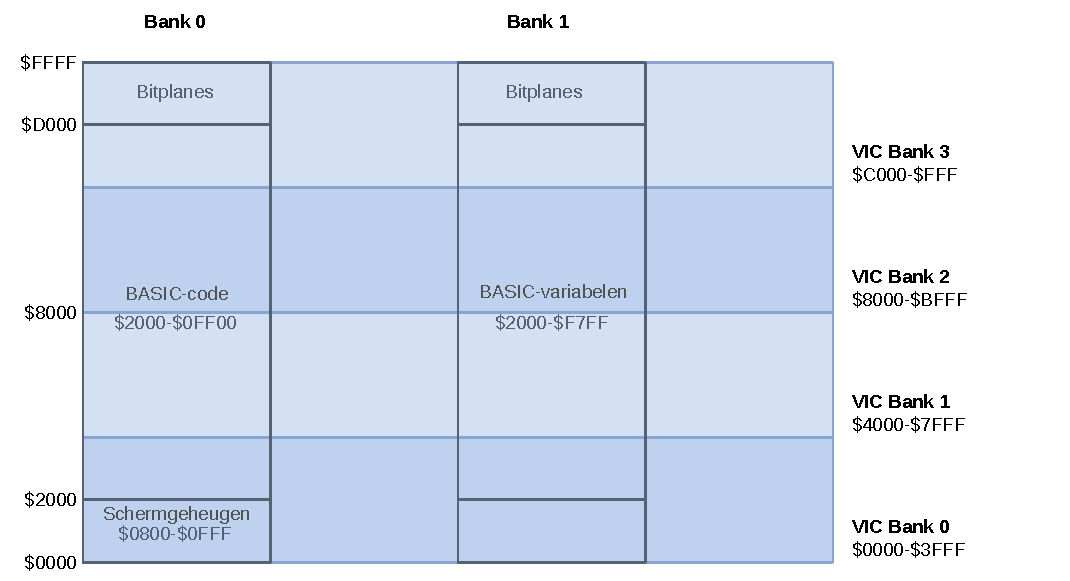
\includegraphics[width=\linewidth]{dutch/images/graphics/vic-banks.pdf}

Los van de VIC is het geheugenbeheer van de Commodore 65 of MEGA65 iets complexer dan dat van het vorige model. Dat komt doordat er in de machine meer geheugen beschikbaar is: bij de Commodore 65 waren 128KB gepland (mogelijk uit te breiden tot 1MB), terwijl de MEGA65 wordt geleverd met 384KB chip-RAM + 8MB zolder-RAM (mogelijk uit te breiden tot 256MB). Zoals eerder vermeld, kan de processor niet het hele geheugenbereik adresseren. Er is slechts 64KB zichtbaar. Om die reden is het geheugen verdeeld in blokken van elk 64KB en deze blokken worden ``banken'' genoemd.

Het systeem kan tot 16 banken hebben en bepaalde banken hebben daarnaast ook specifieke taken. Bank 0 en 1 zijn RAM, wat betekent dat u er zowel kunt lezen als schrijven, terwijl bank 2 en 3 ROM zijn en niet zo eenvoudig te overschrijven.

Bank 0 (gezien vanuit het besturingssysteem BASIC 65 dat start wanneer u de computer inschakelt) heet de systeembank. Deze bevat onder meer de volgende gebieden:

\begin{itemize}
  \item Het schermgeheugen, welke het geheugenbereik \$0800-\$2000 beslaat (standaard)  \item In het geheugen gemapte VIC-registers (indien deze zijn ingemapt, wat standaard het geval is)
\end{itemize}

Overigens staat de implementatie van BASIC65 zelf in ROM (bank 3), terwijl het BASIC van de C64 eveneens in ROM staat (bank 2).

Wilt u meer weten over geheugenbeheer in het algemeen, kijk dan bij \bookvref{cha:memory-map}. In BASIC is de situatie helaas nog complexer. Direct na het inschakelen van de computer bevindt u zich in Bank 128, een speciale bank met een speciale geheugenconfiguratie. U kunt het commando BANK gebruiken om tussen banken te wisselen. Een probleem daarbij is dat u gemakkelijk het overzicht verliest over wat er in welke bank staat of in welke bank u op dat moment werkt. Het is eigenlijk iets eenvoudiger wanneer u in machinetaal werkt. Voor meer informatie over het BANK-commando en over banken in het algemeen raadpleegt u \bookvref{BASIC 65 Commands!BANK}. Houd er rekening mee dat u eerst iets over banken moet weten voordat u op veilige wijze PEEK, POKE of SYS kunt gebruiken. Anders vraagt u zich misschien af waarom uw programma zich niet zo gedraagt als u verwachtte. Wij komen hier later op terug. Terug naar de grafiek.

Laten we beginnen met het schrijven van een eenvoudig BASIC-programmaatje om hires-bitmapgrafiek weer te geven. Indien u dit hoofdstuk tot op dit punt zorgvuldig heeft gevolgd, zult u geen moeite hebben met het begrijpen van de volgende coderegels:

\begin{screencode}
10 POKE $D020,0 : POKE $D021,0          :REM MAAK SCHERM ZWART
20 POKE $D031, PEEK($D031) AND 127      :REM STEL RESOLUTIE IN
30 POKE $DD02, 3                        :REM MAAK VIRTUALE CIA-2 LEES- EN SCHRIJFBAAR
40 POKE $$DD00, PEEK($DD00) AND 252 OR 2:REM KIES VIDEOBANK 1
\end{screencode}

Zoals u op de afbeelding op de vorige bladzijde heeft gezien, verdeelt de VIC-chip het geheugen in 4 videobanken van elk 16KB. Het is belangrijk te begrijpen dat u geen register van de VIC gebruikt om de videobank binnen (geheugen-)bank 0 te definiëren; in plaats daarvan gebruikt u de databits 0 en 1 van \$DD00 of decimaal 56576. Dit was ooit een register van de CIA-2-chip in de Commodore 64, maar in uw MEGA65 is het geïmplementeerd als virtueel register. De ``voorbereiding'' die nodig is om de videobank in te stellen, gebeurt in regel 30, terwijl in de daaropvolgende regel de videobank zelf wordt ingesteld. Overigens geldt: als u de decimale waarde 3 (regel 30) omzet naar binair formaat, is dat 00000011 en dat bewijst dat de databits 0 en 1 op 1 staan, zodat lezen en schrijven is geactiveerd.

{\small
\begin{tabular}{|c|c|l|l|}
	\hline
	Bits & VIC-bank & Geheugengebied & BASIC \\
	\hline
	 \textbf{00} & 3 & \$C000-\$FFFF & ... AND 252 OR 0 :REM AND 11111100 OR 000000\textbf{00} \\
	 \textbf{01} & 2 & \$8000-\$BFFF & ... AND 252 OR 1 :REM AND 11111100 OR 000000\textbf{01} \\
	 \textbf{10} & 1 & \$4000-\$7FFF & ... AND 252 OR 2 :REM AND 11111100 OR 000000\textbf{10} \\
	 \textbf{11} & 0 & \$0000-\$3FFF & ... AND 252 OR 3 :REM AND 11111100 OR 000000\textbf{11} \\
	\hline
\end{tabular}
}

De tabel toont welke bits moeten worden ingesteld om een videobank te selecteren.

\input{dutch/sprites}
\input{dutch/sound}

\part{CPU EN GEHEUGEN}

\chapter{Kennismaken met de 45GS02-CPU}
\label{cha:introducing-the-45gs02-cpu}

Aan dit hoofdstuk wordt nog gewerkt.

\begin{itemize}
\item Hoe werkt een CPU\item Kenmerken van de 45GS02
\end{itemize}

\section{Werken met de monitor}

\begin{itemize}
    \item wat is een machinetaalmonitor\item MONITOR-commando\item registers bekijken\item geheugen bekijken\item code disassembleren\item code assembleren\item een subroutine uitvoeren\item onderbreken en hervatten
\end{itemize}

\section{CPU-instructies}

\begin{itemize}
    \item Instructies\item Adresseermethoden
\end{itemize}

\begin{itemize}
    \item Registers en statusvlaggen\item Geheugen lezen en schrijven\item Berekeningen uitvoeren\item Vertakkingen en subroutines\item MAP en EOM
\end{itemize}

\section{CPU-registers}

\begin{itemize}
    \item Accumulatorregister\item X, Y, Z\item Programmateller\item Stackpointer\item Base-Page (B)\item Statusvlaggen; het statusregister\item MAP
\end{itemize}

\section{De Base-Page}

\begin{itemize}
    \item Doel: snel tijdelijk geheugen; pointers\item Zero-Page\item Het B-register\item Base-Page-adresseermethoden\item Andere Base-Page-bewerkingen\item KERNAL-overwegingen
\end{itemize}

\section{Indirecte adressering}


\section{Het virtuele 32-bits register}


\section{De stapel}

\begin{itemize}
    \item Waarden op de stapel plaatsen en van de stapel halen\item Subroutine-aanroepen\item 8-bits versus 16-bits stackpointer\item Stackrelatieve adresseermethode
\end{itemize}

\section{Interrupts}

\begin{itemize}
    \item Typen interrupts\item Interruptvectoren\item Interface voor interrupthandlers\item Een voorbeeld zonder de KERNAL\item De KERNAL-IRQ uitbreiden\item Opmerking over het MAP-register
\end{itemize}

\section{Instructies coderen}

\begin{itemize}
    \item Opcodes en operanden\item 32-bits indirecte adresseermethode\item Instructies voor het virtuele 32-bits register
\end{itemize}

\section{De 6502-familie}

\begin{itemize}
    \item 6502 / 6510\item 65C02\item 65CE02 (``4502'') / 4510\item 45GS02
\end{itemize}

% TODO: index terms

\chapter{Programmeren met het geheugen}
\label{cha:programming-with-memory}

Als u programma's in assembleertaal schrijft, is het van cruciaal belang dat u begrijpt hoe het geheugen werkt. Vrijwel elke bewerking heeft op de een of andere manier met het geheugen te maken. Gegevensverwerking vindt in het geheugen plaats en programma's worden in het geheugen opgeslagen en vanuit het geheugen uitgevoerd. Bij een hardware-registerarchitectuur in Commodore-stijl loopt alle in- en uitvoer van de computer via het manipuleren van waarden in het geheugensysteem.

Als u programma's in MEGA65 BASIC schrijft, hoeft u zich nauwelijks met het geheugen bezig te houden. Het BASIC-systeem en de meeste van zijn commando's vertegenwoordigen gegevens als getallen, arrays en strings die in variabelen met een naam zijn opgeslagen. U hoeft nooit te weten hoe die gegevens als enen en nullen worden weergegeven, of welke adressen bij welke gegevens horen. Toch kan inzicht in de werking van het geheugen uw BASIC-programma's naar een hoger niveau tillen. U kunt nieuwe manieren bedenken om de gegevens van uw programma te beheren en u kunt rechtstreeks contact leggen met de MEGA65-hardware. Sommige geavanceerde mogelijkheden van de MEGA65 zijn uitsluitend via geheugenregisters toegankelijk.

Net als verschillende andere systemen in de MEGA65 is het geheugensysteem geavanceerder dan u wellicht verwacht, met meerdere bedrijfsmodi. Wanneer u uw MEGA65 voor het eerst inschakelt, begint deze met een geheugenconfiguratie die bedoeld is om de BASIC 65-omgeving te ondersteunen. Een programma kan het geheugen opnieuw configureren om de mogelijkheden van de MEGA65 volledig te benutten, of om de geheugenomgeving compatibel te maken met een Commodore 64 (zoals \textbf{GO64} doet) of een Commodore 65.

In dit hoofdstuk leert u alles over het geheugensysteem van de MEGA65, met de nadruk op het schrijven van programma's voor de MEGA65 in BASIC en assembleertaal. Volledige beschrijvingen van de geheugenvoorzieningen, inclusief de functies voor achterwaartse compatibiliteit met de C64 en C65, vindt u in de bijlagen.

\newpage
\section{Geheugenbegrippen}
\label{sec:programming-with-memory-concepts}

Een computer voert taken uit door gegevens te manipuleren die in zijn {\em geheugen} zijn opgeslagen. Het computergeheugen bestaat uit vele duizenden cellen, waarvan elke cel één {\em byte} aan gegevens bevat die 256 mogelijke waarden kan vertegenwoordigen. Elke cel heeft een numeriek {\em adres}. Het programma dat het geheugen gebruikt, bepaalt wat voor soort gegevens op elk adres staat. Het programma zelf staat als bytes in het geheugen, als machinetaalinstructies die de CPU uitvoert.

\subsection{Bits, bytes en nibbles}

Een {\em bit} is één enkel digitaal signaal met twee mogelijke waarden: uit of aan. Vaak worden bits met andere bits gecombineerd om meer mogelijke waarden te kunnen vertegenwoordigen. Een byte bestaat uit 8 bits en heeft 256 mogelijke waarden.

Bits en bytes worden vaak gebruikt om getallen weer te geven. Hun waarden worden daarbij vaak beschreven als positieve gehele getallen, ook wanneer zij andere soorten gegevens vertegenwoordigen. Als we het over de bits van een byte hebben, staan die van rechts naar links in oplopende plaatswaarde. Bit 0 is de meest rechtse bit, ook bekend als de ``minst significante'' bit. Bit 7 is de meest linkse bit, ook bekend als de ``meest significante'' bit.\footnote{Zie \bookvref{cha:decimal-binary-and-hexadecimal} voor een volledige uitleg van de binaire en hexadecimale notatie.}

\begin{center}
\begin{tabular}{ccccccccl}
{\bf b\textsubscript{7}} &{\bf b\textsubscript{6}} &{\bf b\textsubscript{5}} &{\bf b\textsubscript{4}} &{\bf b\textsubscript{3}} &{\bf b\textsubscript{2}} &{\bf b\textsubscript{1}} &{\bf b\textsubscript{0}} & \\\huge\texttt{0} &\huge\texttt{1} &\huge\texttt{1} &\huge\texttt{0} &\huge\texttt{1} &\huge\texttt{0} &\huge\texttt{1} &\huge\texttt{1} & = 107 \\\small{}128 &\small{}64 &\small{}32 &\small{}16 &\small{}8 &\small{}4 &\small{}2 &\small{}1 & \\
\end{tabular}
\end{center}

Een {\em nibble} is 4 bits. In de computerarchitectuur verwijst de term ``nibble'' naar één van de twee helften van een byte. De {\em hoge nibble} bestaat uit bits 7 -- 4 en de {\em lage nibble} uit bits 3 -- 0.

\subsection{Hexadecimale notatie}

Hexadecimaal is een talstelsel waarin elk cijfer zestien mogelijke waarden kan aannemen, geschreven met de cijfers 0 -- 9 gevolgd door de letters A -- F. Het is bijzonder handig voor het beschrijven van waarden in het computergeheugen, omdat elk hexadecimaal cijfer een nibble (4 bits) aan gegevens vertegenwoordigt. De 8-bits binaire waarde \texttt{\%01101011} kunt u lezen als de twee nibbles \texttt{0110 1011}, ofwel \$6B in hexadecimale notatie.

Geheugenadressen worden doorgaans in hexadecimale notatie weergegeven. Het computergeheugen is gewoonlijk zo ingedeeld dat de groottes als ronde hexadecimale getallen uit te drukken zijn, zoals \$C000.

\begin{center}
\begin{tabular}{|c|c|c|c|c|c|c|c|c}
\cline{1-3}\cline{5-8}
\$0000 & \$0001 & \$0002 & $\cdots$ & \$0FFE & \$0FFF & \$1000 & \$1001 & $\cdots$ \\
\cline{1-3}\cline{5-8}
\end{tabular}
\end{center}

Ronde hexadecimale getallen komen overeen met veelvoorkomende geheugengroottes:

\begin{center}
\begin{tabular}{rl}
\$0001 & 1 byte \\\$0010 & 16 bytes \\\$0100 & 256 bytes \\\$0400 & 1 kilobyte (1KB = 1024 bytes) \\\$1000 & 4 kilobytes (4KB = 4096 bytes) \\\$4000 & 16KB \\\$10000 & 64KB \\\$100000 & 1 megabyte (1MB = 1024KB) \\
\end{tabular}
\end{center}

De adressering begint bij 0, dus gebieden van deze gebruikelijke groottes beginnen aan de rechterkant doorgaans met ``0''-cijfers en stoppen vlak vóór het begin van het volgende gebied. Het bereik \$2000 -- \$2FFF is bijvoorbeeld 4KB groot.

In BASIC kunt u getallen hexadecimaal invoeren door het dollarteken als voorvoegsel te gebruiken (\$). Om bijvoorbeeld de decimale waarde van een hexadecimaal getal in BASIC weer te geven:

\begin{basiccode}
PRINT $C000
\end{basiccode}

Om een getal in hexadecimale notatie in BASIC weer te geven, gebruikt u de functie {\bf HEX\$()}\index{BASIC 65-functies!HEX\$}:

\begin{basiccode}
PRINT HEX$(127)
\end{basiccode}

Als u in assembleertaal programmeert of een machinetaalmonitor gebruikt, worden adressen en waarden standaard in hexadecimale notatie weergegeven.

Dit boek gebruikt soms een punt (.) om groepen van vier hexadecimale cijfers van elkaar te scheiden, zodat ze gemakkelijker te lezen zijn: FFF.FFFF. Als u een lang adres in een programma of commando invoert, tikt u de punt niet mee. Om FFF.FFFF in BASIC in te voeren, tikt u: \texttt{\$FFFFFFF}

Elk hexadecimaal cijfer vertegenwoordigt een nibble van een waarde. De waarde FFF.FFFF kan met zeven nibbles (28 bits) worden weergegeven.

\subsection{Geheugen met willekeurige toegang}

{\em Random Access Memory} (RAM) is geheugen dat gegevens tijdelijk bevat. Een programma kan deze gegevens lezen en ernaar schrijven. Wanneer de computer wordt uitgeschakeld, gaan deze gegevens verloren. Een programma dat deze gegevens wil bewaren, moet ze opslaan op een apparaat voor langetermijnopslag, zoals een diskette (of de SD-kaart van de MEGA65), voordat de computer wordt uitgeschakeld.

Probeer dit. Typ het volgende commando in bij de \screentext{READY.}-prompt:

\begin{basiccode}
POKE $1800,127
\end{basiccode}

Dit {\bf POKE}\index{BASIC 65-commando's!POKE}-commando slaat de bytewaarde 127 op geheugenadres \$1800 op. Typ nu dit commando in:

\begin{basiccode}
PRINT PEEK($1800)
\end{basiccode}

De {\bf PEEK()}\index{BASIC 65-commando's!PEEK}-functie levert de bytewaarde op die op geheugenadres \$1800 is opgeslagen, in dit geval 127. Het {\bf PRINT}\index{BASIC 65-commando's!PRINT}-commando geeft deze waarde weer.

Schakel uw MEGA65 uit, schakel hem weer in en voer \texttt{PRINT PEEK(\$1800)} opnieuw uit. De waarde in het RAM-geheugen is teruggezet.

\subsection{Alleen-lezen geheugen}

{\em Read-Only Memory} (ROM) bevat gegevens die in de fabriek permanent zijn weggeschreven. Net als andere vintage-microcomputers heeft de Commodore 65 een ROM-chip met de programmacode van het besturingssysteem: BASIC, de KERNAL, routines voor het benaderen van randapparaten en voor het uitvoeren van gangbare berekeningen. ROM-gegevens kunnen niet rechtstreeks door een programma worden overschreven en blijven in de computer staan wanneer de computer wordt uitgeschakeld.

De MEGA65 bevat geen traditionele ROM-chip. In plaats daarvan laadt de MEGA65-Hypervisor (het besturingssysteem dat de voorzieningen van de MEGA65 beheert) de programmagegevens van de ``ROM'' uit een bestand op de SD-kaart naar een gebied in RAM. De Hypervisor beveiligt dat RAM standaard als ``alleen lezen'', waarmee de ROM-chip van een Commodore 65 wordt nagebootst. U kunt het ROM-bestand op de SD-kaart vervangen om te upgraden naar nieuwere versies van de MEGA65-ROM.

Probeer dit. Typ deze commando's in en probeer te voorspellen wat het tweede commando zal weergeven. Wijzig 63 in een ander getal en probeer het daarna opnieuw.

\begin{basiccode}
POKE $2100,63
PRINT PEEK($2100)
\end{basiccode}

Het adres \$2100 weigert een nieuwe waarde te aanvaarden. Een volledige uitleg waarom dit zo is, vergt verschillende begrippen die in dit hoofdstuk worden beschreven. Voorlopig volstaat de opmerking dat het geheugen op adres \$2100 zo is ingesteld dat het zich als ROM gedraagt wanneer het op deze manier wordt benaderd.

\subsection{I/O-registers}

Sommige adressen verwijzen naar speciale geheugencellen die de hardware van de computer gebruikt. Deze staan bekend als {\em I/O-registers}. U kunt met de hardware communiceren door gegevens naar deze adressen te schrijven en eruit te lezen. Op deze manier geven BASIC-commando's grafische beelden weer, spelen ze geluiden en lezen ze joysticks uit: ze lezen waarden uit de I/O-registers en zetten er nieuwe in. (``I/O'' verwijst naar de gegevens die als \emph{invoer} naar en \emph{uitvoer} vanuit deze apparaten gaan.)

Probeer dit commando uit. Vervang 7 door een ander getal tussen 0 en 31.

\begin{basiccode}
POKE $D020,7
\end{basiccode}

De VIC-videochip gebruikt het adres \$D020 om de kleur van de schermrand op te slaan. Het {\bf BORDER}-commando stelt dit register in om hetzelfde effect te bereiken.

\begin{basiccode}
BORDER 7
\end{basiccode}

\subsection{Adressen}

De voorbeelden tot nu toe gebruikten adressen die uit vier hexadecimale cijfers bestaan, zoals \$1800. Elk hexadecimaal cijfer stelt vier bits voor (één nibble), dus een hexadecimaal getal van vier cijfers stelt een 16-bits adres voor. Een dergelijk adres ligt in het bereik \$0000 -- \$FFFF, met 65536 mogelijke adressen. De CPU van de Commodore 64 gebruikt 16-bits adressen om maximaal 64 kilobyte (64KB) geheugen te benaderen. Met andere woorden: de Commodore 64 heeft een \emph{adresruimte} van 16 bits, in het bereik \$0000 -- \$FFFF.

De MEGA65 heeft een adresruimte van 28 bits, in het bereik 000.0000 -- FFF.FFFF. Zulke adressen kunnen als 32-bits waarde worden opgeslagen, waarbij de hoogste nibble op 0 wordt gezet. In hexadecimale notatie zou dat een getal van acht cijfers zijn waarvan het meest linkse cijfer 0 is. (Dit cijfer wordt in de notatie doorgaans weggelaten.)

Het BASIC-commando {\bf POKE} en de functie {\bf PEEK()} kunnen 28-bits adressen gebruiken. Bijvoorbeeld, om eerst een waarde in het RAM op adres 800.0000 op te slaan en deze daarna weer op te halen:

\begin{basiccode}
POKE $8000000,63
PRINT PEEK($8000000)
\end{basiccode}

Dit voorbeeld werkt op de MEGA65 en de DevKit. Het Nexys-bord heeft op dat adres geen RAM en negeert pogingen om er gegevens naartoe te schrijven.

\subsection{16-bits adresvertaling}

Het geheugensysteem van de MEGA65 maakt het programma's mogelijk om met 16-bits adressen naar geheugen te verwijzen. Om het volledige 28-bits adres te bepalen, vertaalt het geheugensysteem het adres volgens regels die het programma zelf kan instellen. Deze vertaling staat ook bekend als {\em hermapping} of, in sommige contexten, als {\em banking}.

16-bits adresvertaling biedt verschillende voordelen. De 45GS02-CPU verwerkt 16-bits adressen sneller dan 32-bits adressen. 16-bits adressen nemen bij het opslaan minder ruimte in het geheugen in. De meeste taken van een programma werken binnen één enkel 64KB-gebied van het geheugen, dus het is vaak handig voor een programma om de geheugenconfiguratie aan het begin van een taak in te stellen en dat gebied vervolgens met 16-bits adressen te benaderen.

Adresvertaling is een veelvoorkomende voorziening in de meeste microcomputers. De Commodore 64 gebruikt geheugenbanking om programma's met uitsluitend 16-bits adressen 64KB RAM {\em en} daarnaast ROM en I/O-registers te laten benaderen. De Commodore 65 was zo ontworpen dat het geheugensysteem via 16-bits adresvertaling op de geheugenindeling van de Commodore 64 kon worden ingesteld en bovendien banking in C64-stijl van ROM en I/O-registers ondersteunde.

De MEGA65 biedt meerdere mechanismen voor adresvertaling. De configuratie van het geheugensysteem is één van de complexere onderwerpen binnen de MEGA65-programmering. Dit hoofdstuk behandelt dit onderwerp in detail.

\subsection{Banken en pagina's}

De adressen van de MEGA65 zijn onder te verdelen in gebieden van 64KB, bekend als {\em banken}. Wanneer een adres in hexadecimale notatie is gegeven, is de bijbehorende bank gemakkelijk te bepalen: de meest linkse cijfers van het adres vormen het banknummer en de vier meest rechtse cijfers wijzen een plaats binnen die bank aan.

\medskip
\begin{center}
\begin{tabular}{m{0.4cm}m{0.4cm}m{0.05cm}m{0.4cm}m{0.4cm}m{0.4cm}m{0.4cm}}
\multicolumn{1}{c}{\huge\texttt{\$}} &\multicolumn{1}{c}{\huge\texttt{3}} &\multicolumn{1}{c}{ } &\multicolumn{1}{c}{\huge\texttt{F}} &\multicolumn{1}{c}{\huge\texttt{D}} &\multicolumn{1}{c}{\huge\texttt{A}} &\multicolumn{1}{c}{\huge\texttt{8}} \\
\cline{2-2}\cline{4-5}
& \multicolumn{1}{c}{\small Bank} & & \multicolumn{2}{c}{\small Pagina} &\multicolumn{2}{c}{ } \\
\end{tabular}
\end{center}
\medskip

Bijvoorbeeld: het adres 3.FDA8 (\$003FDA8) is een adres in bank \$3. Het adres 0.1800 (\$0001800) is een adres in bank \$0. Het adres 880.12AB (\$88012AB) ligt in bank \$880.\footnote{In enkele gevallen is dit beter te begrijpen als ``megabyte \$88, bank \$0, offset \$12AB''.}

Het is belangrijk te onthouden dat, wanneer u een 16-bits adres ziet zoals \$2100, de bank waarnaar dit werkelijk verwijst niet noodzakelijk bank 0 is. Het volledige adres hangt af van de configuratie van het geheugensysteem en van de manier waarop het geheugen wordt benaderd.

Een bank is verder onder te verdelen in gebieden van 256 bytes, bekend als {\em pagina's}. Zoals bij banken is ook de pagina gemakkelijk uit een hexadecimaal adres af te leiden: de pagina wordt gevormd door het vierde en derde cijfer van rechts. Pagina \$1C bestaat bijvoorbeeld uit \$1C00 -- \$1CFF. Het adres \$1CB2 ligt in pagina \$1C.

\subsection{Hoe adressen in het geheugen worden opgeslagen}

Computers verwerken geheugenadressen vaak als gegevens, bijvoorbeeld door adressen op te slaan in RAM of in registers. Een 16-bits adres wordt opgeslagen als twee bytes en een 28-bits adres als vier bytes (waarbij de meest linkse nibble op nul wordt gezet).

Om de bytes van een adres te bepalen, deelt u de hexadecimale cijfers in paren, beginnend bij het {\em meest rechtse} paar. Elk paar cijfers vormt een bytewaarde. Het adres \$853FDA8 kan bijvoorbeeld worden weergegeven door de bytes \$A8, \$FD, \$53 en \$08.

Deze volgorde van de bytes van rechts naar links staat bekend als {\em little-endian-volgorde}. De MEGA65 slaat waarden van meerdere bytes volgens conventie op in little-endian-volgorde. De 45GS02-CPU, de I/O-registers en andere routines verwachten dat adressen op deze manier zijn opgeslagen.\footnote{Er bestaan computers die de tegenovergestelde volgordeconventie hanteren, bekend als {\em big-endian} bytevolgorde. De meeste microcomputers gebruiken de little-endian-conventie.}

Om bijvoorbeeld het 28-bits adres 853.FDA8 op te slaan, heeft u vier bytes geheugen nodig. Om dit op te slaan op geheugenplaatsen 0.1800 -- 0.1803, begint u met het opslaan van de meest rechtse byte (\$A8) op plaats 0.1800. De rest gaat als volgt:

\begin{center}
\begin{tabular}{cccc}
\hline
\multicolumn{1}{|c}{\huge\texttt{A8}} &\multicolumn{1}{|c}{\huge\texttt{FD}} &\multicolumn{1}{|c}{\huge\texttt{53}} &\multicolumn{1}{|c|}{\huge\texttt{08}} \\
\hline
\rotatebox{90}{0.1800 } &\rotatebox{90}{0.1801 } &\rotatebox{90}{0.1802 } &\rotatebox{90}{0.1803 } \\
\end{tabular}
\end{center}

Wanneer een 28-bits adres als vier bytes wordt opgeslagen, blijven de bovenste vier bits ongebruikt. In enkele gevallen gebeurt het dat een 28-bits adres zodanig wordt opgeslagen dat die bits iets anders bevatten. U moet er bij het schrijven van zulke adressen zorg voor dragen dat de bovenste bits de juiste waarden behouden. Dat gebeurt doorgaans met booleaanse logica, waarbij de bovenste bits worden ``gemaskeerd''.

Het volgende BASIC-voorbeeld stelt de variabele \texttt{B} in op \$A9 en werkt die daarna zodanig bij dat de bovenste nibble behouden blijft en de onderste nibble op \$3 wordt gezet. Probeer, voordat u het uitvoert, te raden wat het zal tonen.

\begin{basiccode}
10 B = $A9
20 B = B AND $F0 OR $03
30 PRINT HEX$(B)
\end{basiccode}

De Commodore 65 gebruikt een 20-bits adresruimte en gebruikt daarom soms slechts vijf nibbles (vijf hexadecimale cijfers) om een adres te coderen. In enkele gevallen breidt de MEGA65 dit uit naar 28 bits, door naast een ``bank-nibble'' en twee bytes voor het onderste deel van het adres nog een aparte ``megabyte-byte'' op te slaan. Later in dit hoofdstuk wordt een voorbeeld hiervan uitgelegd.

BASIC 65 bevat commando's om 16-bits waarden als bytes te lezen en te schrijven, zonder dat u zelf expliciet naar de little-endian-volgorde hoeft te converteren. {\bf WPOKE addr,val} stelt {\bf addr} in op de lage byte van {\bf val} en {\bf addr+1} op de hoge byte van {\bf val}. Evenzo leest {\bf WPEEK(addr)} de bytes op {\bf addr} en {\bf addr+1} en levert als resultaat het 16-bits getal op.

\begin{basiccode}
WPOKE $1900,$FFD2
\end{basiccode}

BASIC heeft geen specifieke commando's voor het lezen of schrijven van 32-bits waarden, maar u kunt de 16-bits commando's gebruiken om telkens twee bytes tegelijk te verwerken. Let erop dat u voor elke helft de little-endian-volgorde aanhoudt:

\begin{basiccode}
WPOKE $1802, $0853
WPOKE $1800, $FDA8
\end{basiccode}


\newpage
\section{De 28-bits adresruimte}
\label{sec:programming-with-memory-address-space}

De 28-bits adressen vormen een {\em adresruimte} in het bereik 000.0000 -- FFF.FFFF. Slechts een deel van de adressen is toegewezen aan geheugencellen. Andere adressen zijn toegewezen aan I/O-registers en andere bijzondere apparaten. De overige adressen zijn niet toegewezen; die zijn gereserveerd voor toekomstig gebruik door uitbreidingshardware en toekomstige versies van de computer.

De MEGA65 en de DevKit hebben drie grote gebieden met toegewezen adresruimte:

\begin{itemize}
\item {\bf chip-RAM}, 384KB, in het bereik 000.0000 -- 005.FFFF\item {\bf zolder-RAM}, 8MB, in het bereik 800.0000 -- 87F.FFFF\item {\bf I/O-registers en speciaal RAM}, in het bereik F00.0000 -- FFF.FFFF
\end{itemize}

De overige gebieden van de adresruimte zijn gereserveerd voor toekomstige uitbreidingen en toekomstige modellen. Nexys-borden hebben geen zolder-RAM. Zie \bookvref{cha:memory-map} voor details over de gereserveerde gebieden.

Chip-RAM is de belangrijkste werkruimte van de MEGA65. Het bevat programmacode, de ROM-code van de MEGA65 en ruimte voor variabelen en andere gegevens. Het heet ``chip-RAM'' omdat de CPU het met volledige snelheid kan benaderen. BASIC- en KERNAL-functies maken gebruik van delen van het chip-RAM en ook uw BASIC- en machinetaalprogramma's zullen er uitgebreid gebruik van maken.

Zolder-RAM biedt extra geheugen voor algemeen gebruik, met enkele beperkingen. Doorgaans gebruikt een programma het zolder-RAM via de Direct Memory Access (DMA)-voorziening van de MEGA65 om gegevens tussen het zolder-RAM en het chip-RAM te kopiëren (later beschreven). Het zolder-RAM kan niet rechtstreeks door de VIC-chip worden gebruikt voor grafische gegevens, evenmin kan het rechtstreeks worden gebruikt voor het afspelen van audiosamples (``audio DMA''). De CPU kan code die in het zolder-RAM staat wel uitvoeren, maar die code draait langzamer dan code in het chip-RAM. In het algemeen is het benaderen van zolder-RAM ongeveer tien keer zo langzaam als het benaderen van chip-RAM.

\underline{OPMERKING}: Het Freezer-hulpprogramma van de MEGA65 slaat het zolder-RAM niet op en herstelt het ook niet. In theorie kan een gebruiker een programma starten, de Freezer activeren, een freeze-toestand opslaan en op een later tijdstip een nieuwe sessie starten vanuit die freeze-toestand, met een gewist zolder-RAM als gevolg. In de praktijk zou het onredelijk zijn om programma's zo te schrijven dat zij ervan uitgaan dat het zolder-RAM elk moment kan verdwijnen. De beste tussenoplossing is gebruikers erop te wijzen wanneer een programma het zolder-RAM gebruikt en het gebruik van freeze-toestanden onder bepaalde omstandigheden af te raden. (Het louter activeren van de Freezer verandert het zolder-RAM niet. Alleen het herstellen van een freeze-toestand nadat de computer is uit- en weer ingeschakeld, kan problemen veroorzaken.)

De bovenste I/O-registerruimte is de plaats waar de apparaatregisters en het geheugen voor de Hypervisor-functies permanent thuishoren. De meeste programma's benaderen deze voorzieningen indirect, via de geheugenconfiguratievoorzieningen die later in dit hoofdstuk worden beschreven, met name het kleurengeheugen (colour-RAM) van de VIC, de character-ROM en de I/O-registers van de VIC en de SID. Zie \bookvref{cha:memory-map} voor een gedetailleerde lijst van de bovenste I/O-gebieden.


\newpage
\section{De geheugenindeling van het chip-RAM}

De volgende tabel vat samen hoe KERNAL en BASIC van de MEGA65 het chip-RAM gebruiken.

\setlength{\tabcolsep}{3pt}
\begin{longtable}{|L{1.5cm}|L{1.5cm}|p{6cm}|}
\hline
{\bf{Start}} & {\bf{Einde}} & {\bf{Omschrijving}} \\
\hline
\endfirsthead
\multicolumn{3}{l@{}}{\ldots Vervolgd}\\
\hline
{\bf{Start}} & {\bf{Einde}} & {\bf{Omschrijving}} \\
\endhead
\multicolumn{3}{l@{}}{Vervolgd \ldots}\\
\endfoot
\hline
\endlastfoot
\hline
\small 0.0000 & \small 0.0000 & \multicolumn{1}{p{6cm}|}{Gegevensrichting van de CPU-I/O-poort}\\
\hline
\small 0.0001 & \small 0.0001 & \multicolumn{1}{p{6cm}|}{CPU-I/O-poortgegevens}\\
\hline
\small 0.0002 & \small 0.15FF & \multicolumn{1}{p{6cm}|}{KERNAL-variabelen en -gegevens}\\
\hline
\small 0.1600 & \small 0.1EFF & \multicolumn{1}{p{6cm}|}{Vrij voor gebruik door programma's}\\
\hline
\small 0.1F00 & \small 0.1FFF & \multicolumn{1}{p{6cm}|}{Basispagina voor de bitmapgrafiek van BASIC}\\
\hline
\small 0.2000 & \small 0.F6FF & \multicolumn{1}{p{6cm}|}{BASIC: programmatekst}\\
\hline
\small 0.F700 & \small 0.FEFF & \multicolumn{1}{p{6cm}|}{BASIC: scalare variabelen}\\
\hline
\small 0.FF00 & \small 0.FFFF & \multicolumn{1}{p{6cm}|}{Gereserveerd}\\
\hline
\hline
\small 1.0000 & \small 1.1FFF & \multicolumn{1}{p{6cm}|}{DOS-buffers en -variabelen}\\
\hline
\small 1.2000 & \small 1.F6FF & \multicolumn{1}{p{6cm}|}{BASIC: arrays en strings}\\
\hline
\small 1.F700 & \small 1.F7FF & \multicolumn{1}{p{6cm}|}{Gereserveerd}\\
\hline
\small 1.F800 & \small 1.FFFF & \multicolumn{1}{p{6cm}|}{Venster op het kleurengeheugen}\\
\hline
\hline
\small 2.0000 & \small 2.FFFF & \multicolumn{1}{p{6cm}|}{ROM}\\
\hline
\small 3.0000 & \small 3.FFFF & \multicolumn{1}{p{6cm}|}{ROM}\\
\hline
\hline
\small 4.0000 & \small 4.FFFF & \multicolumn{1}{p{6cm}|}{BASIC-bitmapgrafiek, hulpprogramma's}\\
\hline
\small 5.0000 & \small 5.FFFF & \multicolumn{1}{p{6cm}|}{BASIC-bitmapgrafiek, hulpprogramma's}\\
\hline
\end{longtable}

De ROM-banken zijn in gebieden ingedeeld. De meeste programma's hoeven deze adressen niet rechtstreeks te benaderen.

\setlength{\tabcolsep}{3pt}
\begin{longtable}{|L{1.5cm}|L{1.5cm}|p{6cm}|}
\hline
{\bf{Start}} & {\bf{Einde}} & {\bf{Omschrijving}} \\
\hline
\endfirsthead
\multicolumn{3}{l@{}}{\ldots Vervolgd}\\
\hline
{\bf{Start}} & {\bf{Einde}} & {\bf{Omschrijving}} \\
\endhead
\multicolumn{3}{l@{}}{Vervolgd \ldots}\\
\endfoot
\hline
\endlastfoot
\hline
\small 2.0000 & \small 2.3FFF & \multicolumn{1}{p{6cm}|}{DOS}\\
\hline
\small 2.4000 & \small 2.8FFF & \multicolumn{1}{p{6cm}|}{Gereserveerd}\\
\hline
\small 2.9000 & \small 2.9FFF & \multicolumn{1}{p{6cm}|}{Tekenset A}\\
\hline
\small 2.A000 & \small 2.BFFF & \multicolumn{1}{p{6cm}|}{C64 BASIC}\\
\hline
\small 2.C000 & \small 2.CFFF & \multicolumn{1}{p{6cm}|}{Interface}\\
\hline
\small 2.D000 & \small 2.DFFF & \multicolumn{1}{p{6cm}|}{C64-tekenset (C)}\\
\hline
\small 2.E000 & \small 2.FFFF & \multicolumn{1}{p{6cm}|}{C64 BASIC en KERNAL}\\
\hline
\hline
\small 3.0000 & \small 3.1FFF & \multicolumn{1}{p{6cm}|}{Monitor}\\
\hline
\small 3.2000 & \small 3.7FFF & \multicolumn{1}{p{6cm}|}{C65 BASIC}\\
\hline
\small 3.8000 & \small 3.BFFF & \multicolumn{1}{p{6cm}|}{C65-BASIC-grafische routines}\\
\hline
\small 3.C000 & \small 3.CFFF & \multicolumn{1}{p{6cm}|}{Gereserveerd}\\
\hline
\small 3.D000 & \small 3.DFFF & \multicolumn{1}{p{6cm}|}{Tekenset B}\\
\hline
\small 3.E000 & \small 3.FFFF & \multicolumn{1}{p{6cm}|}{C65 KERNAL}\\
\hline
\end{longtable}

\subsection{Hoe programma's het chip-RAM gebruiken}

De twee meest voorkomende soorten MEGA65-programma's zijn programma's die geheel in BASIC zijn geschreven en programma's die geheel in machinetaal zijn geschreven (via assembleertaal of een gecompileerde taal zoals C of Rust).

Een typisch BASIC 65-programma benadert het geheugen nooit rechtstreeks.\footnote{Commodore 64 BASIC-programmeurs zijn gewend om met {\bf POKE} en {\bf PEEK} het geheugen en de I/O-registers te benaderen voor de meeste functies, zoals beeldweergave, geluid en invoerapparaten. BASIC 65 biedt voor deze functies speciale commando's.} Het programma gebruikt BASIC-commando's en taalonderdelen om variabelen, arrays, strings, geluid, sprites en bitmapgrafiek te bewerken. Het BASIC-systeem gebruikt het volledige chip-RAM om deze voorzieningen te ondersteunen en beheert de geheugenconfiguratie om namens het programma registers te benaderen. Dit vereist dat de ROM, welke door de Hypervisor geladen en beschermd wordt, op zijn plaats blijft.

Een BASIC-programma dat het bitmapgrafieksysteem niet gebruikt, kan de geheugengebieden die aan die voorziening zijn toegewezen, voor andere doelen gebruiken. Dit omvat de gebied 0.1F00 -- 0.1FFF en de volledige banken 4 en 5. Indien u van plan bent bitmapgrafiek te gebruiken, maar toch wat extra chip-RAM voor een ander doel nodig heeft, dan kunt u met het commando {\bf MEM}\index{BASIC Commands!MEM} blokken in bank 4 en 5 reserveren. Het grafieksysteem houdt de gebieden die met {\bf MEM} zijn gereserveerd automatisch vrij, ten koste van minder geheugen voor meer schermen, een hogere resolutie of een grotere kleurdiepte. Voor een beschrijving van het commando {\bf MEM} zie \bookref{BASIC 65 Commands!MEM}.

Sommige BASIC-hulpmiddelen in de directe modus, zoals {\bf RENUMBER}, maken tijdelijk gebruik van geheugen in bank 4 en 5. Een programma dat zijn geheugen bij de start initialiseert, heeft daar geen last van. Interactieve taken bij de \screentext{READY.}-prompt die dat geheugen onaangetast nodig hebben, kunnen erdoor wel verstoord worden.

Een gangbare techniek om vanuit een BASIC-programma geheugen te benutten, is gebruikmaken van het ongebruikte geheugen voor ``programmatekst'' na het einde van de programmagegevens van BASIC in 0.2000 -- 0.F6FF. Indien uw programma dit nodig heeft, houd er dan rekening mee dat sommige grafische commando's van BASIC 65 het geheugen direct na het einde van het programma als tijdelijke opslag gebruiken. Afhankelijk van de lengte van uw programma kunt u doorgaans veilig een hoog adresbereik kiezen voor gebruik door het programma, zoals 0.C000-0.F6FF.

\begin{center}
\begin{tabular}{m{0.14cm}m{0.06cm}m{1.45cm}m{0.21cm}m{1.4cm}m{0.1cm}m{0.1cm}m{3.3cm}m{3.3cm}l}
\cline{1-1}\cline{3-9}
\multicolumn{1}{|l|}{\rotatebox{90}{KERNAL}} & \multicolumn{1}{l}{\ldots} &\multicolumn{1}{|l}{\rotatebox{90}{BASIC}} & \multicolumn{1}{|l}{\rotatebox{90}{DOS}} &\multicolumn{1}{|l}{\rotatebox{90}{BASIC}} & \multicolumn{1}{|l}{\rotatebox{90}{Geres.}} &\multicolumn{1}{|l}{\rotatebox{90}{Kleur}} & \multicolumn{1}{|l}{\rotatebox{90}{ROM}} &\multicolumn{1}{|l|}{\rotatebox{90}{BASIC Graf. }} & \\
\cline{1-1}\cline{3-9}
\rotatebox{90}{\small 0.0000} & \rotatebox{90}{\small 0.1600} &\rotatebox{90}{\small 0.2000} & \rotatebox{90}{\small 1.0000} &\rotatebox{90}{\small 1.2000} & \rotatebox{90}{\small 1.F700} &\rotatebox{90}{\small 1.F800} & \rotatebox{90}{\small 2.0000} &\rotatebox{90}{\small 4.0000} & \rotatebox{90}{\small 5.FFFF} \\
\end{tabular}
\end{center}

Een typisch programma in machinetaal gebruikt het BASIC-systeem helemaal niet en beheert in plaats daarvan zijn eigen geheugen. Het kan een klein BASIC-programmaatje gebruiken om het programma op te starten, maar keert nadat het programma is gestart nooit meer terug naar het systeem. Zo'n programma mag elke regio van het chip-RAM gebruiken die BASIC anders in beslag zou nemen.

Indien het programma de KERNAL aanroept, bijvoorbeeld voor schijffuncties, dan moet het de gebieden van het chip-RAM vermijden die voor gebruik door de KERNAL zijn gereserveerd. Met de rest kan het doen wat het wil.

\begin{center}
\begin{tabular}{m{0.14cm}m{0.06cm}m{1.45cm}m{0.21cm}m{1.4cm}m{0.1cm}m{0.1cm}m{3.3cm}m{3.3cm}l}
\cline{1-1}\cline{4-4}\cline{6-8}
\multicolumn{1}{|l|}{\rotatebox{90}{KERNAL}} & \multicolumn{1}{l}{\ldots} &\multicolumn{1}{l}{\ldots} & \multicolumn{1}{|l|}{\rotatebox{90}{DOS}} &\multicolumn{1}{l}{\ldots} & \multicolumn{1}{|l}{\rotatebox{90}{Geres.}} &\multicolumn{1}{|l}{\rotatebox{90}{Kleur }} & \multicolumn{1}{|l|}{\rotatebox{90}{ROM}} &\multicolumn{1}{l}{\ldots} & \\
\cline{1-1}\cline{4-4}\cline{6-8}
\rotatebox{90}{\small 0.0000} & \rotatebox{90}{\small 0.1600} &\rotatebox{90}{\small 0.2000} & \rotatebox{90}{\small 1.0000} &\rotatebox{90}{\small 1.2000} & \rotatebox{90}{\small 1.F700} &\rotatebox{90}{\small 1.F800} & \rotatebox{90}{\small 2.0000} &\rotatebox{90}{\small 4.0000} & \rotatebox{90}{\small 5.FFFF} \\
\end{tabular}
\end{center}

Als het programma de KERNAL nooit hoeft aan te roepen, kan het de ROM volledig ontgrendelen en verwijderen en zo elke byte van de 384KB chip-RAM voor eigen doeleinden opeisen. Met een techniek die verderop wordt besproken, kunt u, als u niet alle 32KB van het kleurengeheugen van de MEGA65 nodig heeft, het ``venster op het kleurengeheugen'' op 1.F800 herbestemmen als gewoon chip-RAM.

\subsection{De geheugenindeling als contract}

Het MEGA65-project heeft de ROM-code overgenomen uit het onafgemaakte ontwerp van Commodore voor de C65 en heeft tijd en moeite gestoken in het afmaken van onvoltooide voorzieningen en het verhelpen van fouten. Dit project loopt nog door en het MEGA65-team verwacht in de toekomst nieuwe versies van de ROM uit te geven.

Het schrijven van programma's met de MEGA65-ROM verschilt daardoor wezenlijk van het schrijven van programma's met de ROM van de Commodore 64, welke in silicium is geëtst en niet langer wordt doorontwikkeld. Het is belangrijk om code te schrijven die zich houdt aan het gedocumenteerde gedrag dat in deze handleidingen staat beschreven---en niet te vertrouwen op ongedocumenteerd gedrag dat in een toekomstige versie zou kunnen veranderen.

Het is een doel van het project om de geheugenindeling van het chip-RAM in toekomstige versies van de MEGA65-ROM consistent te houden met de tabel hierboven. Om de compatibiliteit met toekomstige versies te waarborgen, doen programma's er verstandig aan ``gereserveerde'' gebieden niet als vrije ruimte te behandelen. Indien een nieuwe modus of voorziening wordt ingevoerd die de geheugenindeling wijzigt, zal het programma die voorziening expliciet moeten aanvragen, zodat oudere programma's die geen gebruikmaken van de nieuwe voorziening op de oorspronkelijke geheugenindeling kunnen rekenen.

Binnen elk blok van de geheugenindeling is slechts van een deel van de adressen gegarandeerd dat het tussen ROM-versies gelijk blijft. Een machinetaalprogramma kan bijvoorbeeld KERNAL-routines aanroepen via adressen in een ``jump table'' (sprongtabel), een reeks vaste adressen in de ROM die gegarandeerd ook in toekomstige versies gelijk blijft.\footnote{De jump table wordt in dit boek nog niet beschreven. De C65 gebruikte dezelfde jump table als de C128, met enkele kleine wijzigingen en tot nu toe heeft de MEGA65-ROM deze niet uitgebreid. Indien een ROM-revisie deze tabel uitbreidt, blijven de bestaande vermeldingen onveranderd. Zie de MEGA65 Wiki voor een lijst: \url{https://mega65.atlassian.net/}}

Behalve waar expliciet gedocumenteerd, is het niet de bedoeling dat programma's KERNAL-variabelen rechtstreeks lezen of wijzigen. Sommige geheugenlocaties, zoals de locatie van het schermgeheugen, kunnen uit registers worden afgeleid (en via registers worden aangepast). (Zie \bookvref{cha:viciv}.)

Het gebied van chip-RAM in 0.1600 -- 0.1EFF wordt gegarandeerd niet gebruikt door de KERNAL en BASIC van de MEGA65. Het gebied 0.1F00 -- 0.1FFF is eveneens beschikbaar indien u het bitmapgrafieksysteem van BASIC niet gebruikt. In de standaardgeheugenconfiguratie is dit gebied als RAM toegankelijk, zodat het geschikt is voor het opslaan van machinetaal en gegevens die vanuit een BASIC-programma benaderd kunnen worden.


\newpage
\section{Geheugen gebruiken vanuit BASIC}

BASIC 65 bevat verschillende commando's voor het benaderen en bewerken van geheugen en voor het aanroepen van machinetaalsubroutines:

\begin{itemize}
\item {\bf POKE adres, waarde} : slaat een waarde op een adres weg\item {\bf WPOKE adres, waarde} : slaat een 16-bits waarde weg beginnend bij een adres\item {\bf PEEK(adres)} : leest een waarde van een adres\item {\bf WPEEK(adres)} : leest een 16-bits waarde beginnend bij een adres\item {\bf BLOAD bestandsnaam [,argumenten...]} : laadt gegevens van een bestand in het geheugen\item {\bf BSAVE bestandsnaam, P begin TO P eind [,argumenten...]} : slaat een geheugengebied op in een bestand\item {\bf SYS adres [,registers...]} : roept een machinetaalsubroutine aan die op een adres is opgeslagen\item {\bf EDMA ...} : transformeert of kopieert grote geheugengebieden snel met behulp van hardwareversnelling
\end{itemize}

Ook de commando's {\bf BOOT} en {\bf WAIT} werken op een of andere manier op het geheugen. Zie de BASIC 65-commandoreferentie voor meer informatie over deze commando's.

\subsection{Hermapping van adressen door BASIC}

U is het wellicht opgevallen dat de adressen uit de BASIC-commando's {\bf POKE} die aan het begin van dit hoofdstuk zijn beschreven, allemaal verwijzen naar gebieden van chip-RAM die in de geheugenindeling staan aangeduid als ``Vrij voor gebruik door programma's'' of ``BASIC: programmatekst''. Toch lijken ze zich anders te gedragen:

\begin{itemize}
\item \texttt{POKE \$1800,127} gedraagt zich als RAM: het stelt het geheugen op het adres in en het geheugen kan worden gelezen met \texttt{PRINT PEEK(\$1800)}.\item \texttt{POKE \$2010,63} gedraagt zich als ROM: een poging om het geheugen in te stellen blijft zonder gevolg en het lezen van het geheugen met \texttt{PRINT PEEK(\$2010)} geeft de oorspronkelijke ROM-waarde terug.\item \texttt{POKE \$D020,7} gedraagt zich als een I/O-register: het verandert onmiddellijk de kleur van de rand. Deze waarde kan weliswaar worden gelezen met \texttt{PRINT PEEK(\$D020)}, maar als geheugen is die niet bruikbaar, omdat de randkleur met de waarde meeverandert.
\end{itemize}

\newpage

De commando's en functies van BASIC 65 behandelen adressen in het bereik \$0000 -- \$FFFF volgens bijzondere hermappingregels, ook wel {\em banking} genoemd. In de standaardmodus hermapt BASIC 65 deze adressen als volgt:

\begin{center}
\begin{tabular}{|c|c|c|}
\hline
{\bf 16-bits adresblok} & {\bf Gemapt adresblok} & {\bf Type} \\
\hline
\$0000 -- \$1FFF & 0.0000 -- 0.1FFF & chip-RAM \\
\hline
\$2000 -- \$3FFF & 3.2000 -- 3.3FFF & ROM \\
\hline
\$4000 -- \$5FFF & 3.4000 -- 3.5FFF & ROM \\
\hline
\$6000 -- \$7FFF & 3.6000 -- 3.7FFF & ROM \\
\hline
\$8000 -- \$9FFF & 3.8000 -- 3.9FFF & ROM \\
\hline
\$A000 -- \$BFFF & 3.A000 -- 3.BFFF & ROM \\
\hline
\$C000 -- \$CFFF & 2.C000 -- 2.CFFF & ROM \\
\hline
\$D000 -- \$DFFF & FFD.3000 -- FFD.3FFF & MEGA65-I/O\\
\hline
\$E000 -- \$FFFF & 3.E000 -- 3.FFFF & ROM \\
\hline
\end{tabular}
\end{center}

Benadert u bijvoorbeeld de I/O-registers via \$D000 -- \$DFFF, dan benadert u in feite de I/O-registers in het bovenste gebied van de adresruimte. Deze twee BASIC-commando's zijn gelijkwaardig:

\begin{basiccode}
POKE $D020,7

POKE $FFD2020,7
\end{basiccode}

Het BASIC-systeem zelf gebruikt chip-RAM rechtstreeks, volgens de geheugenindeling van het chip-RAM. BASIC slaat programmatekst bijvoorbeeld op vanaf 0.2000 in het chip-RAM, hoewel de BASIC-functie \texttt{PEEK(\$2000)} in de standaardmappingmodus vanaf 3.2000 leest.

De hermapping van adressen door BASIC 65 geldt alleen voor adressen in het bereik \$0000 -- \$FFFF. Gebruikt u een adres van \$10000 of hoger met {\bf POKE} of {\bf PEEK()}, dan benadert het commando dat chip-RAM-adres rechtstreeks. {\bf SYS} ondersteunt ook lange adressen, zij het met beperkingen (later besproken).

U kunt de adreshermapping van BASIC sturen met het commando {\bf BANK}\index{BASIC 65-opdrachten!BANK}. Dit commando accepteert een banknummer als argument, in het bereik 0 -- 5. Adressen in het bereik \$0000 -- \$FFFF die u daarna gebruikt, worden geïnterpreteerd als offsets binnen die bank. Om bijvoorbeeld de waarde 63 naar adres 0.2010 in het chip-RAM te schrijven:

\begin{basiccode}
BANK 0
POKE $2010,63
\end{basiccode}

Het {\bf BANK}-mechanisme kan alleen met de banken 0 -- 5 worden gebruikt. Het zolder-RAM en de bovenste I/O-registers zijn ermee niet te bereiken.

Om de adreshermapping van BASIC weer in te schakelen, voert u {\bf BANK} uit met het argument 128. Dit getal verwijst niet naar een bank in het geheugen. In plaats daarvan houdt het in dat het commando {\bf BANK} de adresvertaling weer volgens de tabel hierboven activeert.

\begin{basiccode}
BANK 128
POKE $D020,9
\end{basiccode}

{\bf BANK} beïnvloedt elk BASIC-commando en elke BASIC-functie die een adres als parameter accepteert. Dit omvat {\bf PEEK}\index{BASIC 65-functies!PEEK}, {\bf POKE}\index{BASIC 65-commando's!POKE}, {\bf WAIT}\index{BASIC 65-commando's!WAIT}, {\bf BOOT}\index{BASIC 65-commando's!BOOT}, {\bf BSAVE}\index{BASIC 65-commando's!BSAVE} en {\bf BLOAD}\index{BASIC 65-commando's!BLOAD}. {\bf SYS} gaat ook op een bijzondere manier met {\bf BANK} om.

\subsection{BANK en SYS}

Het commando {\bf SYS}\index{BASIC 65-commando's!SYS} voert een machinetaalsubroutine op een opgegeven adres uit. Het behandelt het adres anders dan andere BASIC-commando's en kent enkele beperkingen. Omdat {\bf SYS} de besturing overdraagt aan een eigen routine, moet het extra voorzorgsmaatregelen nemen om te voorkomen dat het systeem de toegang verliest tot het geheugen dat BASIC nodig heeft.

Concreet gebruikt {\bf SYS} de {\bf BANK}-instelling alleen voor adressen in het bereik \$2000 -- \$7FFF. Andere adressen gaan altijd naar het RAM van bank 0, naar KERNAL ROM of naar de I/O-registers, als volgt:

\begin{tabular}{|l|l|}
\hline
{\bf Adresbereik} & {\bf SYS-bestemming} \\
\hline
\$0000 -- \$1FFF & RAM in bank 0 \\
\hline
\$2000 -- \$7FFF & Adres volgens de {\bf BANK}-instelling \\
\hline
\$8000 -- \$BFFF & RAM in bank 0 \\
\hline
\$C000 -- \$CFFF & Character ROM, of bank 0 (ROMC-bit van \$D030) \\
\hline
\$D000 -- \$DFFF & I/O-registers, of bank 0 (bankingregister \$01 in C64-stijl) \\
\hline
\$E000 -- \$FFFF & KERNAL ROM in bank 3 \\
\hline
\end{tabular}

{\bf SYS} negeert bit 7 van de {\bf BANK}-instelling. \texttt{BANK 128} is gelijkwaardig aan \texttt{BANK 0} in het geval van {\bf SYS}. Dit verschilt van {\bf PEEK}, {\bf POKE} en dergelijke, welke op \$2000 -- \$BFFF met \texttt{BANK 128} ROM-code te zien krijgen.

\begin{basiccodesmall}
BANK 128
SYS $1800     : rem Roept de subroutine op 0.1800 aan
SYS $7000     : rem Roept de subroutine op 0.7000 aan
SYS $FFD2,65  : rem Roept de KERNAL-ROM-routine aan
              : rem (met een argument)

BANK 1
SYS $1800     : rem Roept de subroutine in bank 0 op 0.1800 aan
SYS $7000     : rem Roept de subroutine in bank 1 op 1.7000 aan
SYS $FFD2,65  : rem Roept de KERNAL-ROM-routine op 3.FFD2 aan
              : rem (met een argument)
\end{basiccodesmall}

{\bf SYS} kan ook een adres groter dan \$FFFF aanvaarden dat naar een locatie in de banken 1 -- 5 verwijst. Deze adressen hebben echter dezelfde beperkingen als bij het gebruik van {\bf BANK}. Alleen de offsets \$2000 -- \$7FFF binnen de bank verwijzen werkelijk naar het geheugen van die bank, zoals adres \$47000 in bank 4. Voor andere offsets gedraagt het commando {\bf SYS} zich volgens de tabel (RAM in bank 0, ROM of I/O-registers).

Deze beperking levert het tegenintuïtieve gedrag op dat een lang adres voor {\bf SYS} niet noodzakelijk naar het geheugen op dat adres verwijst en dat meerdere adressen naar dezelfde locatie in het geheugen kunnen verwijzen. \texttt{SYS \$11800} en \texttt{SYS \$41800} gedragen zich beide als \texttt{SYS \$1800}, hetwelk een subroutine op adres 0.1800 in bank 0 aanroept.

\begin{basiccodesmall}
SYS $11800    : rem Roept de subroutine in bank 0 op 0.1800 aan
SYS $41800    : rem Roept de subroutine in bank 0 op 0.1800 aan
SYS $51800    : rem Roept de subroutine in bank 0 op 0.1800 aan

SYS $17000    : rem Roept de subroutine in bank 1 op 1.7000 aan
SYS $47000    : rem Roept de subroutine in bank 4 op 4.7000 aan
SYS $57000    : rem Roept de subroutine in bank 5 op 5.7000 aan

SYS $1FFD2,65 : rem Roept de KERNAL-ROM-routine op 3.FFD2 aan
              : rem (met een argument)
\end{basiccodesmall}

Het commando {\bf SYS} kan niet elk adres benaderen. ROM en I/O-registers verbergen de adresoffsets \$C000 -- \$FFFF in elke bank. De adresoffsets \$0000 -- \$1FFF en \$8000 -- \$BFFF bereiken uitsluitend bank 0 en blijven in de banken 1 -- 5 verborgen.

{\bf SYS} is beperkt tot de banken 0 -- 5. Het kan het zolder-RAM en de hogere geheugenadressen niet benaderen, zelfs niet met lange adressen.

Ondanks deze beperkingen is {\bf SYS} tamelijk krachtig. Het komt vaak voor dat een machinetaalprogramma begint met een kort BASIC-programmaatje, zodat de gebruiker na het laden {\bf RUN} kan typen. Dit programmaatje roept {\bf SYS} aan om de machinetaal te starten die in het geheugen staat na het einde van de BASIC-tekst.

\begin{basiccode}
10 SYS $200F
\end{basiccode}

In vroege versies van de MEGA65-ROM moest u {\bf BANK} eerst op 0 instellen voordat u {\bf SYS} op deze manier aanriep. Dat blijft sowieso een goede gewoonte, zodat het programma kan starten, zelfs als de gebruiker de {\bf BANK}-instelling heeft gewijzigd:

\begin{basiccode}
10 BANK 0:SYS $2014
\end{basiccode}

U kunt {\bf SYS} ook gebruiken om een BASIC-programma uit te breiden met subroutines in machinetaal. Een geschikte locatie voor deze subroutines is het bereik \$1600 -- \$1EFF van bank 0. {\bf SYS} kan deze locatie benaderen, ongeacht de huidige {\bf BANK}-instelling.

\subsection{SYS TO}

Als aanvulling op de beperkingen van de geheugentoegang van het {\bf SYS}-commando kent BASIC 65 een variant, {\bf SYS TO}, met extra mogelijkheden. Deze variant verschilt op de volgende punten van {\bf SYS}:

\begin{itemize}
    \item Zowel {\bf SYS} als {\bf SYS TO} verwachten een adres als eerste argument. {\bf SYS} aanvaardt daaropvolgende positionele argumenten voor het instellen van registers. {\bf SYS TO} aanvaardt benoemde argumenten voor het instellen van registers en voor het benaderen van andere voorzieningen.    \item Een programma kan {\bf SYS TO} gebruiken om een pagina-offset toe te passen op adressen \$2000 tot \$7FFF, zodat een subroutineadres in dat bereik kan verwijzen naar een fysiek adres buiten dat bereik, in een bank.    \item Een programma kan {\bf SYS TO} gebruiken om routines aan te roepen terwijl BASIC actief blijft, bijvoorbeeld om {\bf PLAY}-muziek of {\bf MOVSPR}-spritebeweging soepel te laten doorlopen terwijl de machinetaal wordt uitgevoerd.
\end{itemize}

Om een pagina-offset in te stellen, geeft u het argument \texttt{O} op aan {\bf SYS TO}. De waarde bestaat uit drie nibbles, die met 256 worden vermenigvuldigd (twee nibbles naar links geschoven) om de offset te bepalen. Een offset van \$520 heeft bijvoorbeeld tot gevolg dat bij elk adres in het bereik \$2000 tot \$7FFF een offset van \$52000 wordt opgeteld.

\begin{basiccodesmall}
REM : MAP $2000-$7FFF NAAR $54000-$59FFF,
REM : DAARNA AANROEP $6100 + $52000 = $58100

SYS TO $6100,O($520)
\end{basiccodesmall}

Om een routine aan te roepen terwijl BASIC actief blijft, geeft u het argument \texttt{I} op met de waarde 1. U kunt deze modus gebruiken of een pagina-offset instellen, maar niet beide. Indien u deze modus inschakelt, wisselt de KERNAL-IRQ-handler tussen de MAP van uw programma en de MAP van KERNAL om de BASIC-functies op basis van IRQ's uit te voeren.

\begin{basiccode}
SYS TO $1600,I1
\end{basiccode}


\newpage
\section{Geheugen gebruiken vanuit machinetaal}

Machinetaalprogramma's benaderen geheugen en registers, verrichten berekeningen en beslissen welke code daarna moet worden uitgevoerd. Meer doen ze niet! Een programma verricht invoer/uitvoerbewerkingen, zoals het weergeven van een afbeelding, het afspelen van een geluid of het uitlezen van een joystick, louter door met geheugen en registers te werken.

Elke 45GS02-machinetaalinstructie die met geheugen werkt, ondersteunt één of meer {\em adresseermethoden}, waarin staat hoe de instructie het geheugen benadert. Eén van deze adresseermethoden werkt met volledige 28-bits adressen en leest het volledige adres uit vier opeenvolgende bytes in het geheugen, in little-endian-volgorde. Deze methode is bruikbaar, maar in veel gevallen niet de efficiëntste manier om het geheugen te benaderen: de CPU moet tijd besteden aan het lezen van het 28-bits adres en aan het vinden van de geheugenplaats voor de bewerking.

Adresseermethoden die met 16-bits adressen werken, zijn sneller en ruimtezuiniger dan 28-bits indirecte adressering. Bovendien gebruikt de CPU 16-bits adressen om te verwijzen naar de plaatsen van machinetaalinstructies: de CPU slaat het adres van de volgende instructie (de {\em programmateller}) op als een 16-bits waarde en de instructies \texttt{jmp} en \texttt{jsr} gebruiken 16-bits adressen.

Om het mogelijk te maken elke geheugenplaats met een 16-bits adres te benaderen, houdt de 45GS02-CPU een {\em geheugenindeling} bij, welke 16-bits adressen aan 28-bits adressen koppelt. Uw programma kan de geheugenindeling wijzigen met behulp van een register met een speciale functie, bekend als {\em het MAP-register}. Het instellen van het MAP-register vereist het uitvoeren van een reeks speciale CPU-instructies.

Bij de MEGA65 beïnvloeden drie andere mechanismen eveneens de adresvertaling van 16-bits geheugenadressen:

\begin{itemize}
\item ROM- en I/O-banking van de Commodore 64, bestuurd door de CPU-registers op de adressen \$0000 en \$0001\item ROM-banking van de Commodore 65, met behulp van een register op adres \$D030\item Cartridgegeheugen: indien er een cartridge in de uitbreidingspoort is geplaatst, maken aanvullende regels de datalijnen van de cartridge beschikbaar op specifieke 16-bits adresbanken
\end{itemize}

Machinetaalprogramma's die voor de MEGA65 zijn geschreven, kunnen voor de geheugentoegang volledig op het MAP-register vertrouwen en kunnen de geheugenconfiguratieregisters van de C64 en C65 op hun standaardinstellingen laten. Wanneer de betrokken gebieden van 16-bits adressen voor andere doeleinden nodig zijn, heeft MAP voorrang op de andere mechanismen.

Deze sectie beschrijft de geheugentoegang met 45GS02-adresseermethoden en het MAP-register. De overige mechanismen voor het mappen van geheugen komen verderop in dit hoofdstuk kort aan de orde. Zie \bookvref{sec:addressing-modes} voor een volledige beschrijving van de adresseermethoden en \bookvref{cha:45gs02} voor een gedetailleerde uitleg van de bankingmechanismen.

\subsection{Het MAP-register}

Het MAP-register koppelt 16-bits adressen aan 28-bits adressen met behulp van een {\em offset}, een waarde die bij het 16-bits adres wordt opgeteld om het uiteindelijke adres te berekenen.

Stel bijvoorbeeld dat uw programma met een 16-bits adresseermethode geheugen op adres \$4855F moet benaderen. Een mogelijke geheugenindeling is dan om aan het adresgebied \$2000 -- \$3FFF een offset van \$45200 toe te wijzen. Met deze configuratie benadert het 16-bits adres \$335F het werkelijke adres \$4855F in bank 4.

\begin{center}
\begin{tabular}{ccccc}
\$335F & + & \$45200 & = & \$4855F \\\vtop{\hbox{16-bits}\hbox{adres}} & & offset & &
\vtop{\hbox{werkelijk}\hbox{adres}} \\
\end{tabular}
\end{center}

Het MAP-register hermapt telkens blokken van 8KB (\$2000) uit de 16-bits adresruimte. Het MAP-register kan twee offsets opslaan: één voor blokken in het bereik \$0000 -- \$7FFF (``MAPLO'') en één voor blokken in het bereik \$8000 -- \$FFFF (``MAPHI''). Ook slaat het voor elk blok van 8KB een selectievlag op, welke aangeeft of de offset op dat blok moet worden toegepast.

Elk adresblok van 8KB is ofwel ``ongemapt'' of gebruikt de MAP-offset voor zijn helft (MAPLO of MAPHI). Alle gemapte adresblokken in dezelfde helft moeten dezelfde offset delen.

\begin{center}
\begin{tabular}{c|c|c|c|c|l}
MAPLO: & \$6000 -- \$7FFF & \$4000 -- \$5FFF & \$2000 -- \$3FFF & \$0000 -- \$1FFF & \\& 0 & 0 & {\bf 1} & 0 & = \$2 \\
\hline
MAPHI: & \$E000 -- \$FFFF & \$C000 -- \$DFFF & \$A000 -- \$BFFF & \$8000 -- \$9FFF & \\& {\bf 1} & 0 & {\bf 1} & {\bf 1} & = \$B \\
\end{tabular}
\end{center}

De selectievlaggen en de offset voor MAPLO en MAPHI worden tezamen gecodeerd als vier bytes: twee voor MAPLO en twee voor MAPHI. De eerste nibble bevat de selectievlaggen voor de vier blokken van het gebied. Let op de volgorde van de vlagbits: de hogere bits horen bij de hogere adresblokken.

Om bijvoorbeeld uitsluitend het blok \$2000 -- \$3FFF te selecteren, stelt u de MAPLO-selectievlag in op het binaire getal ``0 0 1 0'', dat gelijk is aan het hexadecimale cijfer \$2.

De overige drie nibbles vormen de bovenste drie hexadecimale cijfers van de offset. Om de offset \$45200 voor de geselecteerde MAPLO-blokken te gebruiken, stelt u de overige bits van MAPLO in op \$452. Voor dit voorbeeld is de volledige MAPLO-waarde \$2452.

\begin{center}
\begin{tabular}{cc|cc}
\multicolumn{2}{c}{MAPLO} & \multicolumn{2}{c}{MAPHI} \\X & A & Z & Y \\
\hline
\$s\textsubscript{lo} o\textsubscript{1} &\$o\textsubscript{2} o\textsubscript{3} &\$s\textsubscript{hi} o\textsubscript{1} &\$o\textsubscript{2} o\textsubscript{3} \\
\hline
\$24 & \$52 & \$B3 & \$00 \\
\end{tabular}
\end{center}

De offset moet een veelvoud van 256 bytes (\$100) zijn. De 4510-CPU uit de Commodore 65, waarop de 45GS02 van de MEGA65 is gebaseerd, ondersteunt offsets tot \$FFF00. Hierdoor kan elk 8KB-blok overal in het chip-RAM op een grens van 256 bytes worden hermapd, inclusief mogelijke toekomstige RAM-uitbreidingen tot 1MB. (De 45GS02 biedt ook een manier om grotere offsets in te stellen; die wordt verderop besproken.)

Om het MAP-register in te stellen, laadt u de gecodeerde bytes voor MAPLO en MAPHI in de vier CPU-registers X, A, Z en Y en roept u daarna de instructies {\bf MAP} en {\bf EOM} (``end of MAP'') aan. Let op de volgorde waarin de registers hun waarden toegewezen krijgen. Om MAPLO in te stellen, laadt u X met de selectievlaggen en de bovenste nibble van de offset en laadt u A met de onderste nibbles van de offset. Om MAPHI in te stellen, laadt u Z en Y overeenkomstig.

\begin{asmcode}
LDA #$52   ; MAPLO = selecteer $2 offset $45200
LDX #$24
LDY #$00   ; MAPHI = selecteer $B offset $30000
LDZ #$B3
MAP
EOM
\end{asmcode}

Sommige assemblers kennen de EOM-instructie niet. U kunt in plaats van EOM de NOP-instructie gebruiken, welke dezelfde codering gebruikt. Assemblers die 65CE02-instructies ondersteunen, gebruiken voor MAP de AUG-instructie.

De MAP-instelling blijft actief totdat deze wordt gewijzigd. Houd er rekening mee dat KERNAL-routines afhankelijk zijn van de standaard-MAP-instelling. Herstel daarom de oorspronkelijke geheugenindeling voordat u de KERNAL aanroept.

Als het optellen van de offset bij het 16-bits adres een waarde oplevert die groter is dan het grootste 20-bits adres (\$FFFFF), kapt de optelling de overloopbit af, waardoor het 20-bits adres ``omslaat''. Dit maakt het mogelijk om een negatieve offset toe te passen, opgegeven als tweecomplement. Om bijvoorbeeld het 16-bits adres \$8000 te mappen op het 20-bits adres \$02000, stelt u de offset in op \$FA000 (negatief \$06000).

\subsection{Het MAP-register bekijken}

U kunt de waarde van het MAP-register bekijken met de Matrix Mode-debugger, een seriële console die de Hypervisor van de MEGA65 aanbiedt. Om de Matrix Mode-debugger op de MEGA65 te openen, houdt u \megasymbolkey ingedrukt en drukt u op \specialkey{TAB}. (Druk nogmaals op \megasymbolkey + \specialkey{TAB} om af te sluiten.) Met de juiste hardware kunt u deze console ook bereiken via een seriële UART- of JTAG-verbinding. Gebruik in Matrix Mode het commando {\bf R}, of druk gewoon op \specialkey{RETURN}, om alle registers te bekijken, waaronder MAPHI en MAPLO.\footnote{Zie \bookvref{sec:matrix-mode} voor meer informatie over de Matrix Mode-debugger.}

Om dit in werking te zien, doet u het volgende:

\begin{enumerate}
\item Start de MEGA65-monitor met het commando {\bf MONITOR}.\item Assembleer het volgende machinetaalprogramma op adres \$1800 door de eerste regel als volgt in te typen: \texttt{A1800 LDA \#\$52} De monitor berekent voor elke regel de daaropvolgende adressen. Druk na de laatste regel op \specialkey{RETURN} zonder er een instructie achter te typen.

\begin{asmcode}
LDA #$52
LDX #$24
LDY #$00
LDZ #$B3
MAP
EOM
JMP $180A
\end{asmcode}

\item Roep deze routine aan met de ``jump''-commando van de monitor: \texttt{J1800} De MEGA65 komt in een oneindige lus terecht en keert niet uit de aanroep terug, zodat deze schijnbaar vastloopt.\item Open de Matrix Mode-debugger: houd \megasymbolkey ingedrukt en druk op \specialkey{TAB}.\item Druk op \specialkey{RETURN} om een nieuwe set registers te tonen. Let op de waarden van \texttt{MAPH} en \texttt{MAPL}.
\end{enumerate}

\underline{OPMERKING}: De MAP-instructie wijzigt de waarde van het MAP-register onmiddellijk. Zorg ervoor dat u de geheugenindeling niet wijzigt voor het geheugen waarin de code staat die de geheugenindeling wijzigt! Als de geheugenindeling verandert voor het adres van de code zelf, bereikt de uitvoering de EOM-instructie nooit.

\subsection{MAP en interrupts}

Wanneer een CPU-interrupt optreedt, onderbreekt de CPU de uitvoering van het programma en roept daarna een interrupt-handlerroutine aan. De adressen van de interrupt-handlerroutines (de interrupt-{\em vectoren}) staan op de 16-bits adressen \$FFFA -- \$FFFF en zijn zelf eveneens 16-bits adressen.

De geheugenindeling beïnvloedt zowel de plaats van de vectoren als de adressen van de handlers. Om uw code de kans te geven de geheugenindeling te herstellen zonder onderbroken te worden, schakelt de MAP-instructie interrupts uit (vergelijkbaar met SEI) en schakelt de EOM-instructie interrupts weer in (vergelijkbaar met CLI). Dit geldt ook wanneer interrupts al zijn uitgeschakeld op het moment dat MAP wordt aangeroepen: EOM schakelt interrupts weer in. Indien nodig kan uw programma tussen MAP en EOM nog extra instructies uitvoeren.

De standaardgeheugenindeling houdt de KERNAL-ROM van de MEGA65 gemapt op \$E000 -- \$FFFF. Dit omvat de KERNAL-interrupt-handlerroutines en hun vectoradressen. Als uw programma de KERNAL-interrupt-handlerroutines actief houdt, moet het ervoor zorgen dat \$E000 -- \$FFFF gemapt is op 3.E000 -- 3.FFFF (met een MAPHI-offset van \$30000), zolang interrupts zijn ingeschakeld.

\subsection{28-bits adressen in machinetaal gebruiken}

De 45GS02-CPU bevat een adresseermethode waarmee 28-bits adressen rechtstreeks benaderd kunnen worden, zonder 16-bits adresvertaling. Hoewel deze modus technisch gezien meer CPU-cycli vergt om uit te voeren, weegt het gemak die kosten vaak op bij het benaderen van losse adressen in het bovenste geheugen of van geheugen via pointers, in vergelijking met het gebruik van het MAP-register. Deze modus omzeilt bovendien banking en hermapping, waardoor een programma een MAP-registerwaarde kan behouden die mogelijk door andere code wordt gebruikt.

De Base-Page Quad Indirect Z-Indexed-adresseermethode benadert een 28-bits adres dat als vier bytes op de Base-Page is opgeslagen. Deze methode is een uitbreiding van de Base-Page Indirect Z-Indexed-modus, welke een 16-bits adres benadert dat als twee bytes is opgeslagen.

In een assembler die 45GS02-uitbreidingen ondersteunt, zoals de ACME-assembler, gebruikt u voor de Quad Indirect-modus vierkante haken rond het eerste Base-Page-adres waarop het adres is opgeslagen:

\begin{asmcode}
; Selecteer Base-Page $1600.
; (Dit behoudt de compatibiliteit met de KERNAL, die
; Base-Page $0000 reserveert.)
LDA #$16
TAB

; Bewaar adres 810.4AB0 op Base-Page-adres $40-$43.
; (Vergeet niet de little-endian-volgorde te gebruiken.)
LDA #$B0
STA $40
LDA #$4A
STA $41
LDA #$10
STA $42
LDA #$08  ; (Het meest linkse cijfer is nul.)
STA $43

; Laad de accumulator met de byte op 810.4AB0 (met
; een Z-index van nul).
LDZ #$0
LDA [$40],Z
\end{asmcode}

Deze modus wordt gecodeerd als een gewone Base-Page Indirect-modus, voorafgegaan door een NOP-instructie. Als uw assembler de notatie met vierkante haken niet ondersteunt, kunt u het op deze manier schrijven, met ronde haakjes in plaats van vierkante haken:

\begin{asmcode}
LDZ #$0
NOP
LDA ($40),Z
\end{asmcode}

Zie \bookvref{cha:45gs02} voor meer informatie over adresseermethoden.

Dit is in essentie de manier waarop het BANK-systeem van BASIC werkt. Indien BANK op 0 -- 5 is ingesteld, of een programma een adres benadert dat groter is dan \$FFFF, gebruiken commando's zoals POKE en PEEK de Base-Page Quad indirect Z-geïndexeerde adresseermethode, waarbij het volledige adres wordt weggeschreven naar een locatie die in de Base-Page van de KERNAL is gereserveerd. Dit omzeilt de adresvertaling zonder dat de geheugenconfiguratie gewijzigd hoeft te worden. (Het commando SYS doet iets complexers en daardoor kent het ongewone beperkingen.)


\newpage
\section{Videogeheugen van de VIC-IV}

De videocontroller van de VIC-IV leest geheugen om te bepalen wat er op het scherm moet worden weergegeven, zoals tekens, bitmapgrafiek, sprites en kleurgegevens. Een programma wijzigt de weergave door deze geheugengebieden bij te werken. De geheugenlocaties die voor deze doeleinden worden gebruikt, kan het programma met behulp van I/O-registers aanpassen.

De VIC-IV kan uitsluitend chip-RAM benaderen. Technisch gezien kan de VIC-IV de eerste 16MB van de adresruimte benaderen. De bestaande modellen van de MEGA65 bieden 384KB chip-RAM, met ruimte voor toekomstige uitbreiding.

Deze sectie beschrijft enkele VIC-IV-voorzieningen die met het geheugensysteem te maken hebben. De volgende beschrijvingen gelden niet voor de VIC-II-compatibiliteitsmodus. Zie \bookvref{cha:viciv} voor een volledige beschrijving van de VIC-IV.

\subsection{Schermgeheugen vinden}

De VIC-IV leest de inhoud van het scherm (tekens of pixels) uit een aaneengesloten gebied van het geheugen. Registers bepalen de beginlocatie van dit geheugen. De inhoud en de grootte van het schermgeheugen hangen af van de weergavemodus.

Het startadres van het schermgeheugen neemt 28 bits in beslag, hoewel er slechts 20 bits nodig zijn om een chip-RAM-adres op te slaan. Het 28-bits adres wordt verspreid over de vier bytes \$D060 -- \$D063. De hoogste nibble van het adres staat in de lagere nibble van \$D063, welke voor adressen tot 005.FFFF altijd nul is.

Om het schermgeheugen bijvoorbeeld te laten beginnen op 4.26F0 in bank 4 van het chip-RAM:

\begin{center}
\begin{tabular}{|c|c|c|c|}
\hline
SCRNPTRLSB & SCRNPTRMSB & SCRNPTRBNK & SCRNPTRMB \\\$D060 & \$D061 & \$D062 & \$D063 (laagste 4 bits) \\
\hline
\$F0 & \$26 & \$04 & \$0 \\
\hline
\end{tabular}
\end{center}

\begin{asmcode}
LDA #$F0
STA $D060
LDA #$26
STA $D061
LDA #$04
STA $D062

; Voor de volledigheid: wis bits 0-3 van SCRNPTRMB. De
; MEGA65 heeft geen door de VIC benaderbaar geheugen boven
; 005.FFFF, dus dit is niet nodig indien de vorige
; waarde naar een geldig adres wees.
LDA $D063
AND #$F0   ; wis bits 0-3
STA $D063
\end{asmcode}

Indien u hiermee experimenteert in de MEGA65-monitor, houd er dan rekening mee dat de BASIC-editor de nieuwe schermlocatie niet automatisch gebruikt nadat u deze heeft gewijzigd. U kunt blind typen om het geheugen in te stellen en zo zien dat de nieuwe locatie in gebruik is. Druk op \specialkey{RUN\\STOP} + \widekey{RESTORE} om terug te zetten.

Indien uw programma naar het schermgeheugen schrijft zonder dit register te initialiseren, lees dan de locatie van het schermgeheugen uit het register. Ga niet uit van de oorspronkelijke waarde. De 80x50-weergavemodus, welke de gebruiker kan selecteren door op \specialkey{ESC} \specialkey{5} te drukken, gebruikt een andere locatie voor het schermgeheugen dan de standaard 80x25-weergavemodus.

\subsection{Tekengegevens vinden}

Bij gebruik van een tekensweergavemodus interpreteert de VIC de schermgegevens als schermcodes van tekens. De pixelgegevens voor elk teken worden gelezen uit een tekenset die in het geheugen staat. Registers bepalen het startadres van de geselecteerde tekenset.

De grootte en de indeling van de tekengegevens hangen af van de tekensweergavemodus. De standaardtekstmodus leest tekengegevens als acht bytes per teken, één regel monochrome pixels per byte, voor in totaal 512 mogelijke schermcodes (4KB).

Het startadres van de tekenset wordt als drie bytes opgeslagen in \$D068 -- \$D06A. Om bijvoorbeeld de tekenset op 3.D000 te selecteren:

\begin{center}
\begin{tabular}{|c|c|c|}
\hline
CHARPTRLSB & CHARPTRMSB & CHARPTRBNK \\\$D068 & \$D069 & \$D06A \\
\hline
\$00 & \$D0 & \$03 \\
\hline
\end{tabular}
\end{center}

De ROM-gegevens bevatten drie monochrome tekensets (gebruikt door het BASIC-commando {\bf FONT}):

\begin{itemize}
\item 2.9000: Tekenset A, de C64-tekenset met kleine ASCII-letters\item 3.D000: Tekenset B, een gestileerde set die op een ASCII-terminal lijkt\item 2.D000: Tekenset C, de C64-PETSCII-tekenset (de standaard)
\end{itemize}

Uw programma kan elk van de ingebouwde tekensets naar eigen wens aanpassen door het 4KB-gebied naar RAM te kopiëren en de CHARPTR-registers dienovereenkomstig in te stellen.

De tekengenerator van de VIC-IV kent nog een andere manier om tekengliefen intern op te slaan. Stelt u CHARPTR in op de speciale waarde \$001000, dan gebruikt de VIC-IV 4KB aan intern tekengeheugen waarin de standaard-PETSCII-tekenset is opgeslagen. Zo kunt u alle drie de ROM-regio's voor tekensets een andere bestemming geven zonder de toegang tot de PETSCII-tekenset te verliezen.

\subsection{Spritegeheugen vinden}

De VIC-IV ondersteunt acht hardwaresprites. Naar de afbeeldingsgegevens van deze sprites wordt verwezen door een reeks spritepointers. Anders dan de VIC-II van de Commodore 64 ondersteunt de VIC-IV het verplaatsen van de spritepointers en de afbeeldingsgegevens naar een willekeurige plaats in chip-RAM. De VIC-IV is standaard voor een deel compatibel met de VIC-II, waardoor extra registerbits nodig zijn om de verplaatsing volledig in te schakelen.

Bij de VIC-IV kunnen ook de spritepointers zelf overal in het chip-RAM staan. De locatie van de spritepointers wordt opgeslagen in de registers op \$D06C -- \$D06E. Dit adres moet uitgelijnd zijn op een grens van 16 bytes: wanneer u het adres in hexadecimale notatie uitschrijft, moet het meest rechtse cijfer een 0 zijn. Het adres \$2C60 is bijvoorbeeld uitgelijnd op een grens van 16 bytes.

Bit 7 van \$D06E vertelt de VIC-IV dat de spritepointers 16 bits (twee bytes) breed zijn. Indien de bit niet is gezet, gaat de VIC-IV uit van waarden van 8 bits (één byte) voor de pointers, net zoals de VIC-II.

De waarde van een spritepointer is het adres van de beeldgegevens van de sprite, gedeeld door 64. Deze ongewone eigenschap stelde de VIC-II oorspronkelijk in staat om spritegegevens binnen een bereik van 16KB te lokaliseren aan de hand van een waarde van één byte. De VIC-IV houdt deze eigenschap vanwege de compatibiliteit in stand en staat bovendien toe dat deze waarde 16 bits breed is. Eén gevolg van dit ontwerp is dat het adres van een sprite-afbeelding moet zijn uitgelijnd op een gebied van 64 bytes binnen een pagina: de twee meest rechtse hexadecimale cijfers van een spriteadres moeten \$00, \$40, \$80 of \$C0 zijn.

Om bijvoorbeeld de spritepointers te verplaatsen naar 0.3200 en 16-bits pointerwaarden in te schakelen:

\begin{center}
\begin{tabular}{|c|c|c|c|}
\hline
SPRPTRADRLSB & SPRPTRADRMSB & SPRPTRBNK & SPRPTR16 \\\$D06C & \$D06D & \$D06E (0-6) & \$D06E (7) \\
\hline
\$00 & \$32 & \$00 & +\$80 \\
\hline
\end{tabular}
\end{center}

\begin{asmcode}
LDA #$00
STA $D06C
LDA #$32
STA $D06D
LDA #$80
STA $D06E
\end{asmcode}

Om de eerste sprite beeldgegevens op adres 4.3100 te laten gebruiken, stelt u de 16-bits pointer in op 4.3100 / 64 = \$10C4 (in little-endian-volgorde):

\begin{asmcode}
LDA #$C4
STA $3200
LDA #$10
STA $3201
\end{asmcode}

\subsection{Kleurengeheugen}

De VIC-IV stelt een volledig schermbeeld samen uit één set teken- of pixelgegevens in het schermgeheugen en een aparte set kleurgegevens in het kleurengeheugen. In de 80x25-tekstmodus bevatten de eerste 2000 bytes van het schermgeheugen bijvoorbeeld de schermcodes van de tekens en zijn de eerste 2000 bytes van het kleurengeheugen de kleuren van die tekens.

De VIC-IV heeft 32KB geheugen dat speciaal voor kleurgegevens is gereserveerd en dat alle mogelijke schermmodi kan ondersteunen. U kunt dit geheugen rechtstreeks benaderen via de hogere geheugenadressen FF8.0000 -- FF8.7FFF.

Voor het gemak zijn de eerste 2KB van het kleurengeheugen ook zichtbaar op de adressen 1.F800 -- 1.FFFF. Dit adresvenster in bank 1 laat zich niet via de geheugenconfiguratie uitschakelen: het benadert altijd de eerste 2KB van het kleurengeheugen.

Vanwege achterwaartse compatibiliteit is de eerste 1KB van dit venster, samen met de I/O-registers, ook opgenomen in de banking op \$D800 -- \$DBFF. Bit 0 van het bankingregister van de VIC-III op \$D030 (signaalnaam ``CRAM2K'') breidt dit uit tot de volledige 2KB, als \$D800 -- \$DFFF.

Het startadres van het kleurengeheugen van de VIC-IV is met een register in te stellen, als offset binnen de gebied FF8.0000 -- FF8.7FFF van het kleurengeheugen. Indien u niet alle 32KB van het kleurengeheugen voor uw schermweergave nodig heeft, kunt u het startadres verschuiven en het begin van het kleurengeheugen voor andere doelen gebruiken.

Om bijvoorbeeld het begin van het kleurengeheugen met 2KB te verschuiven, stelt u het register in op \$0800 (in little-endian-volgorde):

\begin{center}
\begin{tabular}{|c|c|}
\hline
COLPTRLSB & COLPTRMSB \\\$D064 & \$D065 \\
\hline
\$00 & \$08 \\
\hline
\end{tabular}
\end{center}

Het verschuiven van het startadres verschuift {\em noch} het venster op het kleurengeheugen op 1.F800, {\em noch} de banking van het kleurengeheugen op \$D800. Verschuift u het begin van het kleurengeheugen met 2KB, dan gebruiken zowel het venster als de I/O-bank de 2KB-gebied die voor de VIC-IV onzichtbaar blijft. Zo kunt u het venster op het kleurengeheugen herbestemmen als RAM voor algemeen gebruik.

Dit BASIC-programmaatje stelt de kleurengeheugen-offset in op 2KB (\$0800) en laat vervolgens zien dat de waarde op \$FF80000 ook zichtbaar is op \$1F800 en \$D800. Ten slotte verandert het de kleur van het eerste teken door \$FF80800 in te stellen.

\begin{basiccode}
10 POKE $D064,0:POKE $D065,8
20 PRINT CHR$(5);CHR$(147);"HALLO DAAR."
30 POKE $FF80000,$BB
40 PRINT HEX$(PEEK($FF80000))
50 PRINT HEX$(PEEK($1F800))
60 PRINT HEX$(PEEK($D800))
70 POKE $FF80800,4
\end{basiccode}


\newpage
\section{Grote geheugenbewerkingen met Direct Memory Access}

In vroege microcomputers voert de CPU alle geheugenbewerkingen uit. Grote geheugenbewerkingen, zoals het kopiëren van een blok geheugen van de ene plaats naar de andere, zijn tijdrovend en leggen de interactie met het programma veelal even stil. Dit beperkt programma's tot kleine geheugenbewerkingen tijdens interactieve taken, zoals spellen en sommige toepassingen.

De Commodore 65 beschikt over specifieke hardware voor het kopiëren en verwerken van grote hoeveelheden geheugen, een systeem dat bekend staat als {\em Direct Memory Access} (DMA). De DMA-hardware voert geheugentaken uit, bekend als {\em taken}. De MEGA65 breidt deze mogelijkheden uit met hogere snelheden en voorzieningen die gespecialiseerd zijn in grafische en audiogegevens.

De DMA van de MEGA65 verschilt op één belangrijk punt van de DMA van de C65 (en van de DMA in andere microcomputers): bij de MEGA65 zit de DMA in de CPU ingebouwd en DMA-taken pauzeren de uitvoering van CPU-instructies. Dat lijkt het doel van specifieke DMA-hardware tegen te werken, ware het niet dat de MEGA65 de DMA-taken in vergelijking met de C65 zeer snel uitvoert, dankzij de hogere maximale CPU-snelheid. Het kopiëren van een grote grafische afbeelding naar het scherm gaat snel genoeg om een vast onderdeel te vormen van de code in de hoofdlus van een spel.

Dit vereenvoudigt ook het programmeermodel: een programma kan een DMA-taak behandelen als een bijzondere soort CPU-instructie, zonder extra logica om te wachten tot de taken klaar zijn. Er bestaat zelfs een methode om de DMA aan te roepen waarbij u de takenlijst voor de DMA rechtstreeks in uw code opneemt, zonder daarvoor extra geheugen te hoeven reserveren. In het algemeen geldt: als de DMA de bewerking ondersteunt die u wilt uitvoeren en de bewerking meer dan acht bytes geheugen omvat, dan is een DMA-taak sneller dan gelijkwaardige CPU-instructies.

Deze sectie introduceert DMA in het kort, als onderdeel van dit overzicht van het geheugen. Voor een volledige beschrijving van de DMA-controller en de uitgebreide voorzieningen van de MEGA65, waaronder grafische en audio-DMA, zie \bookvref{cha:dmagic}.

\subsection{DMA-taken}

Om een DMA-taak uit te voeren, beschrijft u de taak in het geheugen en roept u daarna de DMA aan door het adres van de taakbeschrijving naar de registers te schrijven. De DMA voert de taak uit zodra u de laatste adreswaarde van de taak naar het register schrijft. De CPU onderbreekt zijn werk om de taak uit te voeren en gaat daarna verder met de volgende programmainstructie.

Conceptueel bestaat een taakbeschrijving uit de volgende velden:

\begin{enumerate}
\item Een opdracht: kopiëren of vullen\item Een aantal te verwerken bytes, tot 64KB\item Bij kopiëren: het bronstartadres\item Bij vullen: een vulbyte\item Het bestemmingsstartadres\item De instelling van de wijze waarop de bron- en bestemmingsgebieden moeten worden doorlopen (``adressering'')
\end{enumerate}

Meerdere taken kunnen in één enkele aanroep van de DMA worden beschreven, in de vorm van een ``taaklijst''. De taken worden uitgevoerd in de volgorde waarin ze in de lijst voorkomen.

De MEGA65 breidt het formaat van het C65-DMA-taakrecord uit met een lijst van taakoptietokens. Veel van de uitgebreide voorzieningen van de MEGA65, zoals het kopiëren van afbeeldingsgegevens met transparantie, maken gebruik van taakoptietokens.

\subsection{DMA gebruiken vanuit BASIC}

In BASIC 65 voert het {\bf EDMA}-commando één DMA-taak uit, met beperkte opties. Het {\bf DMA}-commando van de Commodore 65 wordt eveneens ondersteund, maar EDMA verdient de voorkeur voor alle nieuwe programma's die niet op een C65 hoeven te draaien.

Het \textbf{EDMA}-commando aanvaardt vier door komma's gescheiden argumenten: de opdracht (0=kopiëren, 3=vullen), het aantal bytes, ofwel een vulbyte (bij vullen) ofwel een bronstartadres (bij kopiëren) en het bestemmingsstartadres.

\begin{basiccode}
10 SC=WPEEK($D060)+PEEK($D062)*$10000
20 FOR X=32 TO 40
30 EDMA 3,80*25,X,SC
40 GETKEY A$
50 NEXT
\end{basiccode}

De overige DMA-voorzieningen zijn vanuit het \textbf{EDMA}-commando niet eenvoudig te benaderen. Om geavanceerdere DMA-taken uit te voeren, kan een BASIC-programma de taakgegevens met \textbf{POKE} in het geheugen zetten en de taak via de registers aanroepen, zoals hieronder beschreven.

\subsection{DMA gebruiken vanuit machinetaal}

Er zijn verschillende manieren om DMA-taken te beschrijven en te starten, waaronder manieren om programma's te schrijven die compatibel zijn met de Commodore 65. Deze sectie beschrijft twee methoden: het aanroepen van een Enhanced-DMA-taaklijst van de MEGA65 vanuit een gegevensstructuur die op een geheugenadres staat en het aanroepen van een Enhanced-taaklijst die inline in de machinetaal staat. Voor een volledige beschrijving van de opties, inclusief de lijst met de mogelijke MEGA65-taakoptietokens, zie \bookvref{cha:dmagic}.

\subsection{Een Enhanced-taaklijst in het geheugen aanroepen}

Een Enhanced-DMA-taaklijst kan overal in het geheugen staan en kan zowel met een fysiek 28-bits adres worden benaderd als met een 16-bits adres dat via MAP opnieuw is toegewezen.

Om een Enhanced-DMA-taaklijst aan te roepen vanuit een record dat binnen de eerste megabyte van het geheugen staat, schrijft u het adres naar de volgende registers, in deze volgorde:

\begin{enumerate}
\item \$D702: de \emph{bank}-adresbyte, bits 16-22; de hoogste bit wordt genegeerd\item \$D701: de \emph{pagina}-adresbyte, bits 8-15\item \$D705: de laagste adresbyte, bits 0-7
\end{enumerate}

Door de laagste adresbyte naar \$D705 te schrijven, start de uitvoering van de taaklijst, waarbij het adres als een fysiek (niet-gemapt) adres wordt geïnterpreteerd.

Om bijvoorbeeld een Enhanced-DMA-taaklijst aan te roepen die op adres \$42A80 staat:

\begin{asmcodesmall}
LDA #$04
STA $D702
LDA #$2A
STA $D701
LDA #$80
STA $D705    ; De DMA-taaklijst begint met uitvoeren...
\end{asmcodesmall}

De MEGA65 heeft de mogelijkheid om een Enhanced-DMA-taaklijst op een willekeurig 28-bits adres op te slaan. Om een Enhanced-DMA-taaklijst aan te roepen vanuit een record dat op een 28-bits adres staat (zoals een adres in het zolder-RAM), schrijft u het adres naar de volgende registers, in deze volgorde:

\begin{enumerate}
\item \$D702: de \emph{bank}-adresbyte, bits 16-22; de hoogste bit wordt genegeerd\item \$D704: de \emph{megabyte}-adresbyte, bits 20-27; overlapt de bank\item \$D701: de \emph{pagina}-adresbyte, bits 8-15\item \$D705: de laagste adresbyte, bits 0-7
\end{enumerate}

In dit geval liggen de registeradressen \emph{niet} naast elkaar. Vóór de MEGA65 deze voorziening kreeg, bestond er geen ``megabyte''-adresbyte en stelden programma's de ``bank''-adresbyte in zonder de ``megabyte''-adresbyte in te stellen. Om compatibel te blijven met deze programma's, zet het schrijven van de adresbank naar \$D702 de adresmegabyte automatisch weer op nul. Om alle vier de adresbytes te gebruiken, moet u de bank schrijven vóórdat u de megabyte schrijft.

Om de DMA het adres van de taaklijst te laten interpreteren vanuit het gezichtspunt van de CPU op de 16-bits adresruimte, met inachtneming van het MAP-register, schrijft u het laatste lage byte in plaats daarvan naar \$D706.\footnote{De MEGA65 ondersteunt een C65-compatibel DMA-taaklijstformaat, dat een programma kan aanvragen door het lage adresbyte naar \$D700 te schrijven in plaats van naar \$D705 / \$D706. U gebruikt dit uitsluitend als u wilt dat uw programma draait op compatibele C65-prototypehardware. Let op: sommige C65-prototypen hebben een onvolledige DMA-implementatie.} De adressen in de taaklijst zelf zijn nooit gemapte adressen: DMA-taken werken altijd op fysieke adressen. Het gebruik van \$D706 verandert alleen de manier waarop het adres van de taaklijst wordt geïnterpreteerd, namelijk als gemapt 16-bits adres.

Het volgende voorbeeld roept een Enhanced-DMA-taaklijst aan die is opgeslagen onder het label {\tt dmajob}. Voor de volledigheid gebruikt het voorbeeld alle vier de registers, zodat de taaklijst ook naar een hogere megabyte van het geheugen geassembleerd zou kunnen zijn. In de praktijk wordt de meeste programmacode naar de eerste 384KB van het geheugen geassembleerd, zodat het megabyteregister \$D704 kan worden weggelaten.

\begin{asmcodesmall}
LDA #^dmajob
STA $D702
LDA #(dmajob >>> 20)
STA $D704
LDA #>dmajob
STA $D701
LDA #<dmajob
STA $D705  ; De DMA voert direct uit

; Het programma gaat verder...
RTS

dmajob:
!byte $0B, $00       ; tokenlijst
!byte $03, $00, $08  ; vul ($03) $0800 bytes
!byte $BB, $00, $00  ; met waarde $BB
!byte $00, $30, $04  ; beginnend op 4.3000
!byte $00, $00, $00  ; geen rare trucs
\end{asmcodesmall}

Het {\tt \^{}dmajob} hierboven (een dakje gevolgd door een symboolnaam) is de syntaxis van de ACME-assembler voor de bankbyte van het 24-bits adres van het symbool {\tt dmajob}. Pas dit aan naar de syntaxis van uw assembler, of codeer deze waarde vast als u weet in welke bank het {\tt dmajob}-geheugen komt te liggen.

\subsection{Een Enhanced-taaklijst inline in de code aanroepen}

In plaats van eerst een taaklijst in het geheugen op te zetten, kunt u de taaklijst ook inline in uw machinetaal opnemen. Dit is een handige manier om een DMA-taak te schrijven alsof het een CPU-instructie met vooraf vastgestelde waarden is. Gebruik daartoe de instructie \texttt{STA \$D707} (met een willekeurige accumulatorwaarde), gevolgd door assembler-directieven waarmee de gegevensstructuur van de Enhanced-taaklijst wordt geassembleerd. De 45GS02-CPU weet dan dat hij de besturing aan de DMA moet geven en de programmateller voorbij het einde van de DMA-taakgegevens moet zetten.

\begin{asmcodesmall}
STA $D707  ; De DMA voert direct uit
!byte $0B, $00       ; tokenlijst
!byte $03, $00, $08  ; vul ($03) $0800 bytes
!byte $BB, $00, $00  ; met waarde $BB
!byte $00, $30, $04  ; beginnend op 4.3000
!byte $00, $00, $00  ; geen rare trucs

; Het programma gaat verder...
RTS
\end{asmcodesmall}

\subsection{Het formaat van de Enhanced-taaklijst}

Deze sectie presenteert een vereenvoudigde versie van het formaat van de Enhanced-taaklijst. Voor een volledige beschrijving, inclusief de velden die de 45GS02-DMA nog niet ondersteunt en de volledige lijst met taakoptietokens, zie \bookvref{cha:dmagic}.

De {\em taaklijst} is een binair formaat waarin de waarden in bytes zijn verpakt. De lijst bestaat uit één of meer taakrecords, waarbij de ``chain''-bit voor elke taak is gezet, behalve voor de laatste taak in de lijst.

Een Enhanced-{\em taakrecord} bestaat uit een lijst van één of meer taakoptietokens die altijd eindigt met het token ``end of job option list'' (\$00), gevolgd door een gegevensstructuur van 12 bytes. Elk taakoptietoken is een bytewaarde en bij sommige tokens hoort nog een argumentwaarde van één byte. Tenzij u een programma schrijft dat bedoeld is voor een Commodore 65, gebruikt uw tokenlijst doorgaans het token \$0B (zonder argumenten) om het taakrecordformaat van 12 bytes te kiezen.

De structuur van 12 bytes ziet er als volgt uit:

\begin{center}
\begin{tabular}{|c|p{8cm}|}
\hline
{\bf Bytes} & {\bf Inhoud} \\
\hline

\$00 & Opdracht \\& {\bf 1 -- 0}: 00 voor kopiëren, 11 voor vullen \newline{\bf 2}: 0 indien dit de laatste taak in de lijst is, 1 indien de lijst doorloopt \newline{\bf 3}: Interrupts toelaten \\
\hline

\$01 -- \$02 & Aantal (16 bits) \\
\hline

\$03 -- \$05 & Bronadres of vulbyte \\& Vulbyte in \$03 \newline Bronadres (20 bits) in \$03 -- \$05 \newline Hoge bits van \$05: \newline{\bf 6}: Richting: 0 om vanaf de start op te tellen, 1 om vanaf de start af te tellen \newline{\bf 7}: I/O: 1 om tijdens de DMA de I/O-registers op \$D000 -- \$DFFF te benaderen \\
\hline

\$06 -- \$08 & Bestemmingsadres (20 bits) \\& Gebruikt hetzelfde formaat als het bronadres \\
\hline

\$09 & Adresseeropties \\& {\bf 1 -- 0}: Adresseermethode van de bron \newline{\bf 3 -- 2}: Adresseermethode van de bestemming \newline Adresseermethoden: \newline00: Lineair: schuift voor alle bytes vooruit in de aangegeven richting \newline10: Vasthouden: schuift niet op, maar herhaalt alleen het startadres \\
\hline

\$0A -- \$0B & Gereserveerd, altijd ingesteld op \$00 \$00 \\
\hline

\end{tabular}
\end{center}

Bron- en bestemmingsadressen worden in het taakrecord opgeslagen als 20-bits adressen, in little-endian-volgorde. Om de volledige 28-bits adresruimte te kunnen benaderen, gebruikt u de taakoptietokens waarmee de hoogste byte van het startadres (\$80 \$xx) en het bestemmingsadres (\$81 \$xx) wordt ingesteld. Het token geldt voor alle taken in de taaklijst.

Bij het uitvoeren van een keten van meerdere Enhanced-taken heeft elk taakrecord zijn eigen taaktokenlijst. Taaktokens van eerder in de keten gelden voor alle latere taken in dezelfde keten. Om de tokens voor een volgende taak ongewijzigd te laten, gebruikt u één enkele \$00 als taaktokenlijst.

Voorbeeld: het geheugen met de BASIC-programmatekst in zijn geheel kopiëren naar het zolder-RAM.

\begin{asmcodesmall}
dmajob:
!byte $80, $00       ; Hoogste byte van de bron: $00
!byte $81, $80       ; Hoogste byte van de bestemming: $80
!byte $0B            ; Gebruik het taakrecordformaat van 12 bytes
!byte $00            ; Einde van de tokenlijst
!byte $00, $00, $d7  ; kopieer ($00) $d700 bytes
!byte $00, $20, $00  ; vanaf (00)0.2000
!byte $00, $00, $00  ; naar (80)0.0000
!byte $00, $00, $00  ;
\end{asmcodesmall}

Voorbeeld: een keten van drie taken, waarin elke taak een vulbewerking uitvoert.

\begin{asmcodesmall}
dmajob:
!byte $0B, $00       ; tokenlijst
!byte $07, $00, $01  ; vul ($03) $0100 bytes
                     ; ga verder met de taakketen (+$04)
!byte $BB, $00, $00  ; met waarde $BB
!byte $00, $30, $04  ; beginnend op 4.3000
!byte $00, $00, $00  ;

!byte $00            ; tokenlijst (ongewijzigd)
!byte $07, $00, $01  ; vul ($03) $0100 bytes
                     ; ga verder met de taakketen (+$04)
!byte $CC, $00, $00  ; met waarde $CC
!byte $00, $31, $04  ; beginnend op 4.3100
!byte $00, $00, $00  ;

!byte $00            ; tokenlijst (ongewijzigd)
!byte $03, $00, $01  ; vul ($03) $0100 bytes
                     ; einde van de taakketen
!byte $DD, $00, $00  ; met waarde $DD
!byte $00, $32, $04  ; beginnend op 4.3200
!byte $00, $00, $00  ;
\end{asmcodesmall}

DMA-taken negeren alle mapping- en banking-instellingen. U kunt aangeven dat een bron- of bestemmingsadres het gebied \$D000 -- \$DFFF als I/O-registers moet behandelen, door bit 23 van het adresrecord in te stellen.

U kunt een DMA-taak voorstellen als een proces met twee cursors: één voor de bron (bij kopiëren) en één voor de bestemming. De DMA schuift elke cursor volgens de taakbeschrijving vooruit, gedurende evenveel stappen als het aantal aangeeft en kopieert of vult bij elke stap de bestemming.

Adresseermethoden bieden één manier om invloed uit te oefenen op de beweging van de cursors:

\begin{itemize}
\item De {\em lineaire} adresseermethode schuift de cursor bij elke stap één adres op.\item De {\em vasthoudende} adresseermethode schuift de cursor niet op. Deze blijft bij elke stap op het startadres staan.\item De {\em doorlooprichting} geeft aan of er bij elke stap tijdens lineaire adressering wordt opgeteld of afgeteld.
\end{itemize}

Voorbeeld: een kopieerbewerking waarbij de broncursor wordt vastgehouden en de bestemmingscursor lineair opschuift, lijkt op het uitvoeren van een vulbewerking met de byte op het bronadres.

\begin{asmcodesmall}
dmajob:
!byte $0B, $00       ; tokenlijst
!byte $00, $80, $00  ; kopieer ($00) $0080 bytes
!byte $00, $19, $00  ; vanaf 0.1900
!byte $40, $31, $04  ; naar 4.3140
!byte $02, $00, $00  ; houd de bron vast
\end{asmcodesmall}

De uitgebreide DMA van de MEGA65 ondersteunt nog veel geavanceerdere doorlooppatronen, die met taakoptietokens worden aangestuurd. Met de DMA kunt u lijnen en patronen in het scherm- en kleurengeheugen tekenen.

Commodore heeft de implementatie van de DMA van de Commodore 65 beschreven, maar deze nooit voltooid. Omwille van de historie reserveert de MEGA65 bits in het DMA-taakrecord voor deze onvoltooide voorzieningen, ook al kan een implementatie nooit werkelijk compatibel zijn met het prototype van de Commodore 65.


\newpage
\section{Gevorderde geheugenonderwerpen}

\subsection{De geheugenmapping testen met de Matrix Mode-debugger}

In de Matrix Mode-debugger,\footnote{Ter herinnering: om de Matrix Mode-debugger te activeren, houdt u \megasymbolkey ingedrukt en drukt u op \specialkey{TAB}. Zie \bookvref{sec:matrix-mode} voor meer informatie over de Matrix Mode-debugger.} geeft het \texttt{m}-commando de gegevens weer op een opgegeven geheugenlocatie. Om bijvoorbeeld de inhoud van het RAM vanaf adres 0.2000 weer te geven:

\begin{basiccode}
m2000
\end{basiccode}

De debugger leest {\em altijd} vanuit 32-bits adressen en houdt geen rekening met MAP of andere voorzieningen voor geheugenbanking, ook niet wanneer er een adres van vier hexadecimale cijfers wordt opgegeven. Om het gemakkelijker te maken te zien hoe de CPU de 16-bits adressen ziet, plaatst de MEGA65 het gezichtspunt van de CPU op de hogere adressen 777.0000 -- 777.FFFF. Om bijvoorbeeld weer te geven wat de CPU ziet op het 16-bits adres \$2000:

\begin{basiccode}
m7772000
\end{basiccode}

De bank 777 houdt rekening met het MAP-register, evenals met de mechanismen voor het mappen van geheugen die in de volgende secties worden beschreven.

\subsection{Geheugenbanking in C64-stijl}

De 16-bits adressen \$0000 en \$0001 verwijzen naar registers. Deze registers functioneren precies hetzelfde als de CPU-registers die op deze adressen in een Commodore 64 te vinden zijn. Zij regelen het mappen van de C64-ROM in de 16-bits adresruimte, precies zoals dat op een C64 gebeurt.

In een MEGA65 dienen deze registers twee doelen: ze nemen de I/O-registers op \$D000 -- \$DFFF op in de 16-bits adresruimte, zodat deze het chip-RAM overlappen en ze verschaffen in de C64-modus (\textbf{GO64}) toegang tot de C64-versies van BASIC en KERNAL.

Om in de MEGA65-modus de I/O-registers uit de 16-bits adresruimte te halen, zodat de 16-bits adressen \$D000 -- \$DFFF het onderliggende chip-RAM op 0.D000 -- 0.DFFF benaderen, schrijft u \$84 naar locatie \$0001. Om de I/O-registers te herstellen, schrijft u \$85 naar locatie \$0001.

\underline{OPMERKING}: De registers \$0000 en \$0001 zijn uitsluitend schrijfbaar. Ze werken niet met de machinetaalinstructies TRB en TSB.

Dit BASIC-voorbeeld demonstreert hoe u locatie \$D020 eerst als I/O-register (de randkleur) benadert en vervolgens als RAM-adres. Probeer te raden wat het zal tonen voordat u het uitvoert.

\begin{basiccode}
10 POKE $D020,3
20 POKE 1,$84
30 POKE $D020,4
40 X=PEEK($D020)
50 POKE 1,$85
60 PRINT X
70 PRINT PEEK($D020)
\end{basiccode}

Banking in C64-stijl geldt alleen voor adresblokken van 8KB die niet door het MAP-register zijn geselecteerd (``ongemapte'' blokken). Als de banking in C64-stijl bijvoorbeeld de I/O-registers op \$D000 -- \$DFFF heeft liggen en de regio \$C000 -- \$DFFF met een offset van 0 is gemapt, dan benadert het programma het RAM op die locatie en {\em niet} de I/O-registers. De regio \$C000 -- \$DFFF moet ongemapt zijn, wil de CPU toegang tot de I/O-registers hebben.

Op vergelijkbare wijze kunt u het MAP-register gebruiken om het RAM op de adressen 0.0000 en 0.0001 te benaderen, dat gewoonlijk door de bankingregisters in C64-stijl wordt verborgen. Als het MAP-register het adresblok \$0000 -- \$1FFF voor mapping selecteert en een offset van 0 toepast, benaderen de 16-bits adressen \$0000 en \$0001 het RAM op 0.0000 en 0.0001 en niet de bankingregisters in C64-stijl. De bankingregisters in C64-stijl zijn uitsluitend te benaderen wanneer de regio \$0000 -- \$1FFF ongemapt is.

Het is gebruikelijk dat een MEGA65-programma de I/O-registers op \$D000 in de banking laat en het MAP-register gebruikt wanneer het het onderliggende RAM moet benaderen. Zo'n programma hoeft het bankingregister in C64-stijl niet te wijzigen.

\subsection{Het bankingregister \$D030 van de VIC-III}

De Commodore 65 biedt een bankingmechanisme om aanvullende ROM-gegevens met 16-bits adressen toegankelijk te maken. Deze banking wordt bestuurd door het I/O-register \$D030.\footnote{Om het bankingregister van de VIC-III op \$D030 te benaderen, moet de computer de VIC-III/IV-``I/O-persoonlijkheid'' gebruiken, die verderop wordt beschreven. Dit is de standaard in de MEGA65-modus.}

De bits 3, 4, 5 en 7 mappen gebieden van ROM-gegevens in de 16-bits adresruimte volgens deze tabel. (Ter herinnering: bits worden van rechts naar links genummerd vanaf 0, zodat bit 7 de hoogste bit is.)

\begin{center}
\begin{longtable}{|L{1.5cm}|L{1.5cm}|L{1.5cm}|L{1.5cm}|}
\hline
{\bf \$D030-bit} & {\bf Signaalnaam} & {\bf 20-bits adres} & {\bf 16-bits adres} \\
\hline
\endfirsthead
\multicolumn{4}{l@{}}{\ldots Vervolgd}\\
\hline
{\bf \$D030-bit} & {\bf Signaalnaam} & {\bf 20-bits adres} & {\bf 16-bits adres} \\
\endhead
\multicolumn{4}{l@{}}{Vervolgd \ldots}\\
\endfoot
\hline
\endlastfoot
\hline
3 & ROM8 & \$28000 -- \$29FFF & \$8000 -- \$9FFF \\
\hline
4 & ROMA & \$2A000 -- \$2BFFF & \$A000 -- \$BFFF \\
\hline
5 & ROMC & \$2C000 -- \$2CFFF & \$C000 -- \$CFFF \\
\hline
7 & ROME & \$2E000 -- \$2FFFF & \$E000 -- \$FFFF \\
\end{longtable}
\end{center}

Als \$D030 bijvoorbeeld is ingesteld op \$64 = \%01100100, dan is bankingbit 5 gezet en zijn de bits 3, 4 en 7 gewist. Dit betekent dat ROMC is ingeschakeld en dat de 16-bits adressen \$C000 -- \$CFFF 2.C000 -- 2.CFFF benaderen. Dit is de standaardtoestand van \$D030 wanneer u de computer inschakelt.

Net als bij banking in C64-stijl geldt de \$D030-banking alleen voor adresblokken van 8KB die het MAP-register niet voor het toepassen van een offset heeft geselecteerd. Voor ongemapte regio's geldt: indien voor een regio of de ROM-banking in C64-stijl of de \$D030-ROM-banking is ingeschakeld, verwijzen die adressen naar de ROM in bank 2. Elk van deze ROM-bankingmechanismen gebruikt de ROM in bank 2, dus er is geen conflict wanneer beide tegelijk zijn ingeschakeld.

Houd er rekening mee dat \$D030 geen enkele MEGA65-KERNAL-ROM uit bank 3 inmapt. De KERNAL gebruikt zelf het MAP-register om zijn eigen code te benaderen en gebruikt de \$D030-banking uitsluitend om ROM-code op 2.C000 te benaderen met ROMC ingeschakeld. Zoals bij het bankingregister in C64-stijl kan een typisch MEGA65-programma de bankingbits van \$D030 ongemoeid laten en MAP gebruiken om indien nodig RAM of ROM op deze adressen te benaderen.

\subsection{Cartridge-ROM}

Indien er een Commodore 64-cartridge in de uitbreidingspoort is geplaatst, leidt het geheugensysteem de toegang tot delen van de 16-bits adresruimte om naar de lijnen van de poort, welke doorgaans verbonden zijn met de ROM-chips in de cartridge. De cartridge bestuurt twee extra lijnen waarmee zij via de CPU-registers op de adressen \$0000 en \$0001, bekend als EXROM en GAME, verschillende geheugenconfiguraties kan opvragen. Deze configuraties zijn identiek aan die van een Commodore 64. Zie voor meer informatie een naslagwerk over de Commodore 64.

De Commodore 64 herkent dat er een C64-cartridge is geïnstalleerd wanneer één of beide lijnen EXROM en GAME laag (0) zijn. Een typische cartridge in C64-stijl maakt op basis van de waarden van EXROM en GAME één of twee gebieden van 8KB voor het systeem toegankelijk. Als beide lijnen hoog zijn, wordt er geen cartridge-ROM op 16-bits adressen gemapt.

De cartridge-hardware is verbonden met de volledige 16-bits adresbus en kan in beginsel voor alle 65536 adressen waarden teruggeven. Op de MEGA65 is de volledige 64KB aan cartridgeadressen beschikbaar op de daartoe bestemde bovenste adressen 400.0000 -- 400.FFFF.\footnote{De MEGA65 ondersteunt een protocol voor MEGA65-cartridges die automatisch in de MEGA65-modus opstarten. Dit wordt in een latere versie van deze handleiding gedocumenteerd.}

De adresvertaling door het MAP-register heeft voorrang op de geheugenconfiguratie van de C64-cartridge. De mapping van cartridge-ROM overschrijft de geheugenmapping in \$D030-stijl.

\subsection{I/O-persoonlijkheden}

De I/O-registers vormen de belangrijkste manier waarop de KERNAL, de BASIC-interpreter of een machinetaalprogramma met de MEGA65-hardware omgaat. Deze registers gedragen zich als geheugenlocaties waarmee u waarden in de hardware instelt, zoals voor het weergeven van grafische beelden of het voortbrengen van geluid, of waarden uit de hardware leest, zoals gebruikersinvoer op het toetsenbord of de joystick. In BASIC geschreven programma's benaderen deze registers doorgaans indirect via commando's, hoewel zij dit ook rechtstreeks via geheugentoegang kunnen doen.

De MEGA65 start in een configuratie waarmee de meeste van zijn voorzieningen via registers op 16-bits adressen in \$D000 -- \$DFFF beschikbaar zijn. Voor deze registers bestaan er vier verschillende configuraties, bekend als {\em I/O-persoonlijkheden:}

\begin{itemize}
\item {\bf MEGA65}. Schakelt alle voorzieningen van de MEGA65 VIC-IV en de Commodore 65 VIC-III in. Dit is de standaard.\item {\bf Commodore 65}. De VIC-III zonder de VIC-IV-uitbreidingen. Voor C65-compatibiliteit.\item {\bf Commodore 64}. De VIC-II. Wordt gebruikt door de C64-modus (\textbf{GO64}).\item {\bf MEGA65 Ethernet}. Een persoonlijkheid voor een speciaal doel, voor het benaderen van de Ethernet-poort van de MEGA65.
\end{itemize}

De registers van alle vier de persoonlijkheden zijn beschikbaar in de 28-bits adresruimte, in elk 4KB-blok van het bereik FFD.0000 -- FFD.3FFF. Wanneer een bepaalde persoonlijkheid is ingesteld, wordt \$D000 -- \$DFFF gemapt op het overeenkomstige blok van bovenste adressen. De standaard-MEGA65-persoonlijkheid mapt deze adressen bijvoorbeeld op FFD.3000 -- FFD.3FFF. Met 28-bits adressen kunt u alle vier de persoonlijkheden tegelijk benaderen, hoewel u rekening moet houden met wisselwerking tussen deze persoonlijkheden (zoals ``hete registers'' van de VIC).

Let op dat het bankingregister \$D030 niet beschikbaar is in de C64-I/O-persoonlijkheid. Als uw programma in de C64-modus start of op een andere manier naar die I/O-persoonlijkheid omschakelt, moet het eerst omschakelen naar de C65- of MEGA65-persoonlijkheid voordat het dit register benadert.

Een typisch voor de MEGA65 geschreven programma gebruikt de MEGA65-persoonlijkheid en gaat ervan uit dat deze al ingesteld is wanneer het programma start. Zie \bookvref{cha:memory-map} voor informatie over hoe u kunt wisselen van gebruikte persoonlijkheid, bijvoorbeeld om bij het starten van uw programma uit voorzorg de gewenste persoonlijkheid in te stellen.

\subsection{ROM omzetten in RAM}

De MEGA65 bewaart de code voor de KERNAL en de BASIC-interpreter in de banken 2 en 3. Om deze code te beschermen tegen overschrijving door andere programma's, dwingt de MEGA65 af dat deze banken alleen-lezen zijn, waarmee wordt gesimuleerd dat er ROM-chips in Commodore-stijl op die adressen zijn aangesloten. De MEGA65-Hypervisor laadt de ROM-gegevens tijdens het opstarten en beheert de schrijfbeveiliging.

Een programma kan de schrijfbeveiliging van de banken 2 en 3 opheffen om die gebieden als chip-RAM te gebruiken. De meeste programma's hebben niet de hele ROM in het geheugen nodig. Een programma dat in de C65-modus draait, heeft bijvoorbeeld naar alle waarschijnlijkheid geen C64-BASIC-ROM-code nodig. De geheugenindeling van het chip-RAM eerder in dit hoofdstuk beschrijft welke ROM-gebieden voor welk doel worden gebruikt.

Een zorgvuldig geschreven programma dat de ingebouwde routines geheel niet nodig heeft, kan het volledige gebied van 128KB een andere bestemming geven. Zorg er bij het overschrijven van de KERNAL voor dat u interrupts uitschakelt en de vectoren van de interrupt-handlers vervangt.

Om de schrijfbeveiliging van de banken 2 en 3 uit te schakelen, roept u de Hypervisor-trap ROM Write-enable aan ({\tt hyppo\_rom\_writeenable}), als volgt:

\begin{asmcodesmall}
LDA #$02
STA $D641
CLV
\end{asmcodesmall}

Om deze weer in te schakelen gebruikt u op dezelfde manier de trap ROM Write-protect ({\tt hyppo\_rom\_writeprotect}) met {\tt LDA \#\$00}. De instructie na de {\tt STA} moet een instructie met één cyclus zijn, doorgaans {\tt CLV}: de CPU voert die bij het terugkeren uit de Hypervisor al dan niet uit. {\tt NOP} wordt niet aanbevolen, omdat deze op de 45GS02 als prefix voor de volgende instructie kan werken.

Om naar RAM in de banken 2 en 3 te schrijven, moet u het MAP-register, 32-bits instructies of DMA gebruiken. Wanneer banking in C64-stijl of \$D030-banking actief is (en de betreffende 16-bits adressen niet-gemapt zijn), benadert het lezen van die adressen bank 2, terwijl het schrijven naar die adressen in RAM van bank 0 terechtkomt. Dit lijkt op wat er gebeurt wanneer u op een Commodore 64 naar een adres met ROM-banking schrijft.

Om na te gaan of het gebied schrijfbeveiligd is, kunt u eenvoudig proberen er een waarde naar te schrijven. De MEGA65 start op met ingeschakelde schrijfbeveiliging.

Het register \$D640 is alleen beschikbaar in de MEGA65-I/O-persoonlijkheid.

Houd er rekening mee dat dit {\em geen} bankingmechanisme is, zoals dat op een Commodore 64 wel het geval is. Als uw programma de oorspronkelijke ROM-code nodig heeft nadat u die heeft overschreven (bijvoorbeeld om deze te herstellen), kopieert u eerst met DMA de oorspronkelijke ROM naar het zolder-RAM.

\subsection{MAP gebruiken om geheugen op hogere adressen te benaderen}

Zoals eerder besproken, kan het MAP-register elk blok van 8KB hermapen naar een andere locatie in de eerste 1MB van de adresruimte. Dit is handig voor het benaderen van de 384KB chip-RAM, inclusief eventuele toekomstige uitbreidingen. De MAP-instructie komt oorspronkelijk van de 4510-CPU van de Commodore 65, welke ontworpen was voor een adresruimte van 1MB.

De 45GS02-CPU van de MEGA65 breidt het MAP-register uit met de mogelijkheid om elk blok van 256 bytes in de 28-bits adresruimte te benaderen. Dit gebeurt in de vorm van een extra hoge byte (twee nibbles) voor elk van MAPLO en MAPHI. Deze hoge byte dient als bits 20-27 van het uiteindelijke adres.

\begin{center}
\begin{tabular}{ccccc}
\$335F & + & \$45200 & = & \$4855F \\\vtop{\hbox{16-bits}\hbox{adres}} & & offset & &
\vtop{\hbox{gemapt}\hbox{adres}} \\
\\
& & \$80 & $\to$ & \$804855F \\
& & \vtop{\hbox{hoge}\hbox{byte}} & & \vtop{\hbox{uiteindelijk}\hbox{adres}}
\end{tabular}
\end{center}

Merk op dat de hoge MAP-byte de bits 20-27 van het eindadres instelt. Levert de optelling van de offset bij het 16-bits adres een waarde op die groter is dan 20 bits, dan ``rolt'' de optelling over binnen het 20-bits gedeelte van het adres en heeft zij geen invloed op de hoge byte van het eindadres.

U stelt een hoge MAP-byte in door de instructie {\bf MAP} twee keer aan te roepen voordat u {\bf EOM} aanroept. De eerste aanroep stelt de hoge byte in en de tweede aanroep stelt, zoals eerder, de selectievlaggen en de resterende 12 bits van de offset in. De computer schakelt de interrupts automatisch uit tussen de eerste {\bf MAP}-aanroep en de {\bf EOM}-aanroep.

Om de hoge byte in te stellen, laadt u de hoge byte in het A-register voor MAPLO of in het Y-register voor MAPHI. Laadt daarna de speciale waarde \$0F in het X-register voor MAPLO of in het Z-register voor MAPHI. Roep {\bf MAP} aan om de hoge byte in te stellen. Laadt vervolgens de selectievlaggen en de overige offsetwaarden in, roep {\bf MAP} aan en roep tot slot {\bf EOM} aan.

Om bijvoorbeeld \$A000 -- \$BFFF in het zolder-RAM te mappen naar \$8000000 -- \$8001FFF, gebruikt u een offset van \$F6000 en een hoge byte van \$80. Stelt u MAPHI in op deze offset met de selectievlag \$2, dan past de computer de offset op het gewenste blok toe.

\begin{asmcodesmall}
LDA #$00
LDX #$00
LDY #$80  ; MAPHI hoge byte van $80
LDZ #$0F  ; (Bijzondere waarde om de hoge byte in te stellen)
MAP

LDA #$00
LDX #$00
LDY #$60  ; MAPHI-offset: $F60
LDZ #$2F  ; MAPHI-selectievlag: $2 = A000 - BFFF
MAP
EOM
\end{asmcodesmall}

Let op: wijzig de hoge byte van het 32KB-adresgebied waarin de code staat die het mappen uitvoert, niet! De instelling van de hoge byte wordt actief bij de eerste MAP-instructie en als de code per ongeluk wordt weggemapt, kan de programmateller de overige instructies niet meer bereiken, zelfs niet als de uiteindelijke mapping compatibel is.

\underline{OPMERKING}: De hoge MAP-bytes behouden hun waarde totdat ze opnieuw worden bijgewerkt met deze procedure van twee MAP-instructies. Door de procedure van één MAP-instructie worden ze \emph{niet} op nul gezet. De hoge MAP-bytes hebben bij een herstart van de CPU de beginwaarde nul en de KERNAL zet deze bytes niet op een waarde ongelijk aan nul, zodat een programma er in de meeste gevallen vanuit kan gaan dat ze aan het begin van het programma nul zijn. Het volgende voorbeeld zet alle MAP-offsetbytes op nul.

\begin{asmcodesmall}
LDA #$00
LDX #$0F
LDY #$00
LDZ #$0F
MAP        ; MAPHI- en MAPLO-megabyte-offsets zijn nu nul
           ; Schakel interrupts uit

LDA #$00
LDX #$00
LDY #$00
LDZ #$00
MAP        ; MAPHI- en MAPLO-bankoffsets zijn nu nul
EOM        ; Einde MAP, schakel interrupts in
\end{asmcodesmall}

In de meeste gevallen is het voor programma's eenvoudiger om het geheugen op hogere adressen te benaderen via 28-bits adresseermethoden of via DMA. Deze uitgebreide MAP-voorziening is opgenomen voor de volledigheid.

\subsection{Het MAP-register lezen}

De 45GS02-CPU kan het MAP-register instellen met een combinatie van CPU-instructies, maar er is geen manier om het register op dezelfde wijze te lezen als andere CPU-registers. Een programma kan hiervoor echter een Hypervisor-trap gebruiken. De hypervisor-trap {\tt hyppo\_get\_mapping} schrijft de registerwaarden van MAPHI en MAPLO, inclusief de megabyte-offsets, naar zes bytes op een opgegeven plaats in het geheugen.

De geheugenplaats waarnaar de hypervisor-trap deze waarden schrijft, moet op een paginagrens tussen 0.0000 en 0.7E00 liggen. U stelt het Y-register in op de meest significante byte van het beginadres wanneer u de trap aanroept. Om bijvoorbeeld het MAP-register naar het RAM op de adressen 0.6200 -- 0.6205 te kopiëren:

\begin{asmcode}
LDY #$62

LDA #$74
STA $D640
CLV
\end{asmcode}

\subsection{Al het chip-RAM beschikbaar maken}

Met de technieken die in dit hoofdstuk worden beschreven, kunt u het geheugensysteem zodanig configureren dat al het chip-RAM beschikbaar komt op de adressen 0.0000 -- 5.FFFF. Een zorgvuldig geschreven programma kan de volledige machine overnemen, I/O-registers op hogere adressen benaderen en al het chip- en zolder-RAM gebruiken.

Een overzicht van de procedure:

\begin{enumerate}
\item Schakel de interrupts uit.\item Wis alle bits van \$D030.\item Zet het MAP-register volledig op nul.\item Wis de bits 0, 1 en 2 van \$0001 om de I/O-registers uit het bereik \$D000 -- \$DFFF te verwijderen.\item Verschuif het begin van het kleurengeheugen met ten minste \$0800 (2KB) vooruit, zodat het venster op het kleurengeheugen als RAM voor algemeen gebruik kan dienen.\item Hef de ROM-schrijfbeveiliging voor de banken 2 en 3 op met de trap ROM Write-enable ({\tt LDA \#\$02 : STA \$D641 : CLV}).\item Laad aangepaste interrupt-handlercode in bank 0, stel de interruptvectoren in en schakel de interrupts daarna weer in.
\end{enumerate}

Om de eerste 2KB als geheugen voor algemeen gebruik te kunnen benutten, mag het programma alleen weergavemodi gebruiken die ten hoogste 30KB aan kleurgegevens vereisen. Een programma dat alle 32KB van het kleurengeheugen gebruikt, moet de eerste 2KB zichtbaar laten in het venster op het kleurengeheugen op 1.F800 -- 1.FFFF. (Het is niet vereist om dit geheugen in te mappen op \$D800 -- \$DFFF.)

Het programma moet MAP gebruiken om het RAM op 0.0000 en 0.0001 te benaderen, door MAP in te schakelen voor \$0000 -- \$1FFF met een offset van 0.

\subsection{Waarom het SYS-commando slechts bepaalde adressen kan gebruiken}

Eerder in dit hoofdstuk is uitgelegd dat het BASIC-commando {\bf SYS} tegenintuïtieve beperkingen kent op de adressen die het kan benaderen. Dat kunnen we nu volledig verklaren, met behulp van de geavanceerdere begrippen uit dit hoofdstuk.

Voor BASIC-functies en -commando's zoals {\bf PEEK} en {\bf POKE} gebruikt de KERNAL de voorziening voor 32-bits indirecte adressering van de 45GS02 om grote adressen te benaderen. Bij een adres van \$10000 of hoger laadt het commando het volledige adres in een variabele op de Base-Page en roept het vervolgens de 32-bits indirecte adressering aan om het geheugen te benaderen. Bij een adres van \$0000 -- \$FFFF met een {\bf BANK}-instelling van 0 -- 5 gebruikt het commando de {\bf BANK}-instelling als het bovenste deel van het adres. De 32-bits indirecte adressering negeert het MAP-register en de voorzieningen voor geheugenbanking en kan elk adres in de computer benaderen.

Is het adres \$0000 -- \$FFFF en is de {\bf BANK}-instelling 128, dan gebruikt BASIC de 16-bits adresseermethode van de CPU, welke de MAP-registerinstelling van de KERNAL respecteert, evenals de D030-instelling en de instellingen voor geheugenbanking in C64-stijl. Zo benaderen die commando's de ROM en de I/O-registers met \texttt{BANK 128}.

{\bf SYS} draagt de CPU op om code op een plaats in het geheugen uit te voeren. De programmateller van de CPU is een 16-bits register en kan niet, zoals de 32-bits indirecte adressering dat kan, los van het MAP-register en andere voorzieningen voor geheugenmapping grotere adressen benaderen. Als onderdeel van de KERNAL moet de KERNAL-ROM in het geheugen beschikbaar blijven op de 16-bits adressen \$E000 -- \$FFFF, zodat interrupts afgehandeld kunnen worden. Ook moeten de KERNAL-variabelen benaderbaar blijven op de adressen \$0000 -- \$1FFF, zodat de interrupt-handlercode ze kan gebruiken. Code die door {\bf SYS} wordt aangeroepen, kan zelf beslissen of de KERNAL functioneel blijft, maar {\bf SYS} houdt de KERNAL actief voor het gebruikelijke geval waarin de machinetaal de besturing wil teruggeven aan een actief BASIC-programma of aan de \screentext{READY.}-prompt.

De KERNAL gebruikt het MAP-register om de ROM in bank 3 te benaderen. Om de ROM op \$E000 -- \$FFFF te houden, stelt hij de MAPH-offset in op 3 en markeert dat geheugengebied als ``gemapt''. Er is slechts één offset die MAP voor alle 8KB-gebieden in \$8000 -- \$FFFF kan gebruiken, zodat bij de aanvang van een {\bf SYS}-aanroep de overige gebieden in dat bereik ofwel ongemapt moeten zijn en naar bank 0 verwijzen (of de D030/\$01-banking gebruiken), ofwel naar bank 3 gemapt moeten zijn. De meest bruikbare keuze voor {\bf SYS} is om de overige hogere gebieden ongemapt te laten.

Evenzo moet het gebied, om te zorgen dat adressen in het bereik \$0000 -- \$1FFF blijven verwijzen naar het KERNAL-variabelengeheugen in bank 0, ofwel ongemapt zijn ofwel met een offset van nul gemapt zijn. Het ligt voor de hand dat {\bf SYS} dat gebied ongemapt laat, zodat het voor de adressen \$2000 -- \$7FFF andere banken kan benaderen en dat is dan ook wat het doet. {\bf SYS} gebruikt het MAP-register om voor een adres waarvan het onderste woord \$2000 -- \$7FFF is, hogere banken te benaderen, zowel bij gebruik van {\bf BANK} als wanneer een groot adres wordt opgegeven.

Het MAP-register is veel flexibeler dan dit: het maakt het mogelijk om bijna elk adres te bereiken via de 16-bits adressen \$2000 -- \$7FFF, met behulp van een breed scala aan mogelijke offsets. De machinetaal die door {\bf SYS} wordt aangeroepen, moet dan wel zodanig geschreven zijn dat zij weet welke offset er wordt gebruikt. De programmateller zou daarbij relatief zijn ten opzichte van de offset en een {\tt JMP}-instructie in de code zou een adres moeten gebruiken dat op dezelfde offset is gebaseerd. Het is wel mogelijk om machinetaal te schrijven met uitsluitend relatieve spronginstructies (zoals {\tt BRA}), maar historisch gezien heeft het commando {\bf SYS} dat nooit vereist. In plaats daarvan beperkt {\bf SYS} zich tot offsets van 64KB, om het programmeermodel eenvoudig te houden.

\subsection{Hoe SYS TO werkt}

Het commando {\bf SYS TO} kan een pagina-offset toepassen op een adres in het bereik \$2000 -- \$7FFF, om zo meer geheugenplaatsen te benaderen. Nu we weten dat MAP hierbij betrokken is, is dit eenvoudig uit te leggen: het argument \texttt{O} stelt de MAP-offset in voor de onderste helft van de 16-bits adresruimte, waarbij \$2000 -- \$7FFF als te mappen gebied is geselecteerd. Met de pagina-offset kunt u code overal in de eerste 384KB van het geheugen benaderen, zolang de routine zodanig is geschreven dat deze rekening houdt met deze MAP-instelling.

\begin{basiccode}
REM : MAP $2000-$7FFF NAAR $54000-$59FFF,
REM : DAARNA AANROEP $6100 + $52000 = $58100

SYS TO $6100,O($520)
\end{basiccode}

Standaard schakelen {\bf SYS} en {\bf SYS TO} BASIC uit terwijl de machinetaalsubroutine wordt uitgevoerd. Dit omvat het wijzigen van MAP, zodat de KERNAL-ROM niet langer op \$2000 -- \$7FFF en \$8000 -- \$BFFF is gemapt, alsmede het instellen van een interne vlag voor de KERNAL-IRQ-handler, zodat deze geen BASIC-IRQ-voorzieningen meer bedient, zoals {\bf PLAY} en {\bf MOVSPR}. Wanneer de machinetaal terugkeert, herstelt {\bf SYS} de MAP-instelling van KERNAL en schakelt de BASIC-IRQ-voorzieningen weer in.

Het tijdelijk uitschakelen van de BASIC-IRQ-voorzieningen kan voor een BASIC-programma dat van deze voorzieningen afhankelijk is een kortstondige onderbreking veroorzaken, zoals muziekweergave die hapert. Om dit te voorkomen, biedt het commando {\bf SYS TO} een bedrijfsmodus waarin BASIC tijdens de subroutine actief blijft. Het argument \texttt{I1} schakelt deze modus in. Wanneer deze modus is ingeschakeld, geeft {\bf SYS TO} de KERNAL-IRQ-handler opdracht om voor het uitvoeren van de BASIC-functies over te schakelen naar de MAP van KERNAL en daarna terug te schakelen naar de MAP van uw programma.

\begin{basiccode}
SYS TO $1600,I1
\end{basiccode}

{\bf SYS TO} kan niet tegelijkertijd een pagina-offset gebruiken en BASIC actief houden, omdat deze voorzieningen het MAP-register op verschillende manieren gebruiken.

\part{HARDWARE}

\chapter{Nexys4-borden gebruiken als een MEGA65}

\section{Uw eigen MEGA65-compatibele computer bouwen}

U kunt uw eigen MEGA65-compatibele computer bouwen met een Nexys4DDR-bord (ook wel Nexys A7) of een ouder Nexys4-bord (zonder DDR).
Deze bijlage beschrijft het proces om een Nexys4DDR (Nexys A7)-bord hiervoor in te stellen (het nieuwere, bij voorkeur te gebruiken bord).
Het oudere non-DDR Nexys4-bord wordt ook ondersteund en de instructies zijn hetzelfde, met uitzondering van het feit dat u een bitstream moet gebruiken die voor dat bord ontworpen is.
Het gebruik van een Nexys4DDR-bitstream op een non-DDR Nexys4-bord of andersom kan onherstelbare schade aan uw bord veroorzaken. Zorg er daarom voor dat u de juiste bitstream voor uw bord heeft.


DISCLAIMER: M.E.G.A kan geen enkele verantwoordelijkheid aanvaarden voor schade die aan uw Nexys4DDR/NexysA7/Nexys4-borden kan ontstaan.

\newpage

\section{Werkende Nexys4-borden}

Er zijn momenteel drie Nexys FPGA-borden die als MEGA65 ingesteld kunnen worden:

\begin{minipage}{\linewidth}
  \subsection{Het Nexys4-bord}

  Niet meer geproduceerd, maar nog wel verkrijgbaar via sommige websites met oude voorraad.

  \begin{center}
    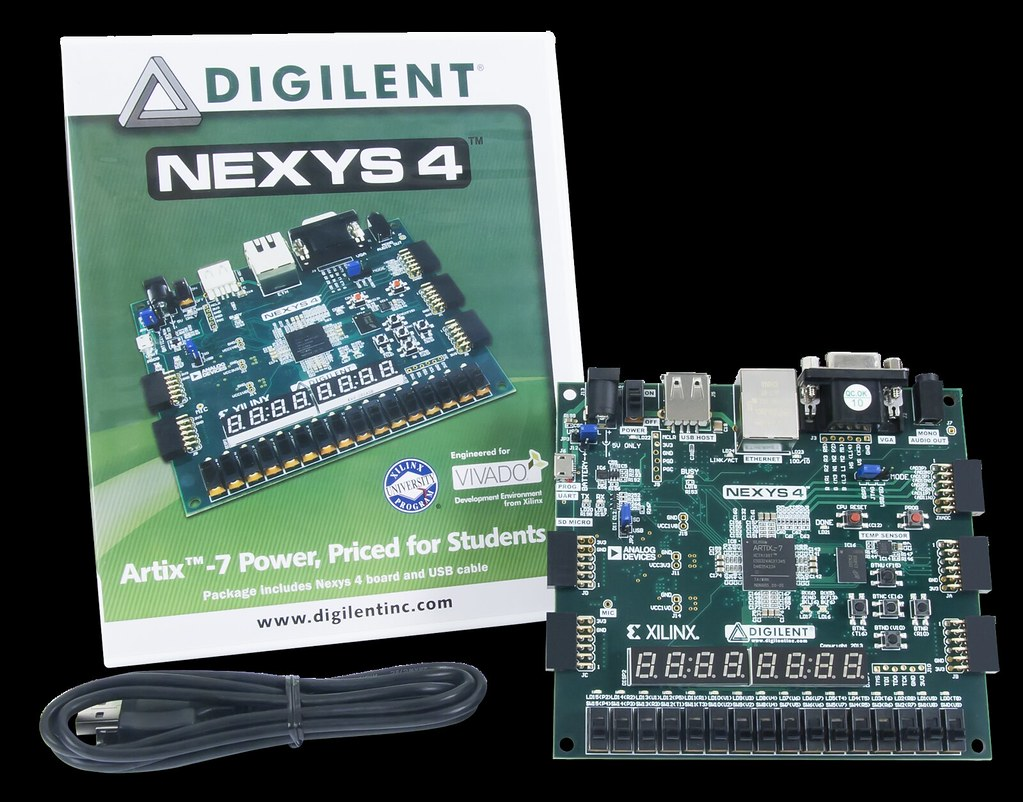
\includegraphics[width=0.4\linewidth]{images/img001_nexys4_board.jpg}
  \end{center}

  Documentatie:

  \begin{itemize}
    \item \url{https://reference.digilentinc.com/reference/programmable-logic/nexys-4/reference-manual}
    \item \url{https://reference.digilentinc.com/\_media/reference/programmable-logic/nexys-4/nexys4\_rm.pdf}
  \end{itemize}
\end{minipage}

\begin{minipage}{\linewidth}
  \subsection{Het Nexys4DDR-bord}

  Niet meer geproduceerd, maar nog wel verkrijgbaar via sommige websites met oude voorraad.

  \begin{center}
    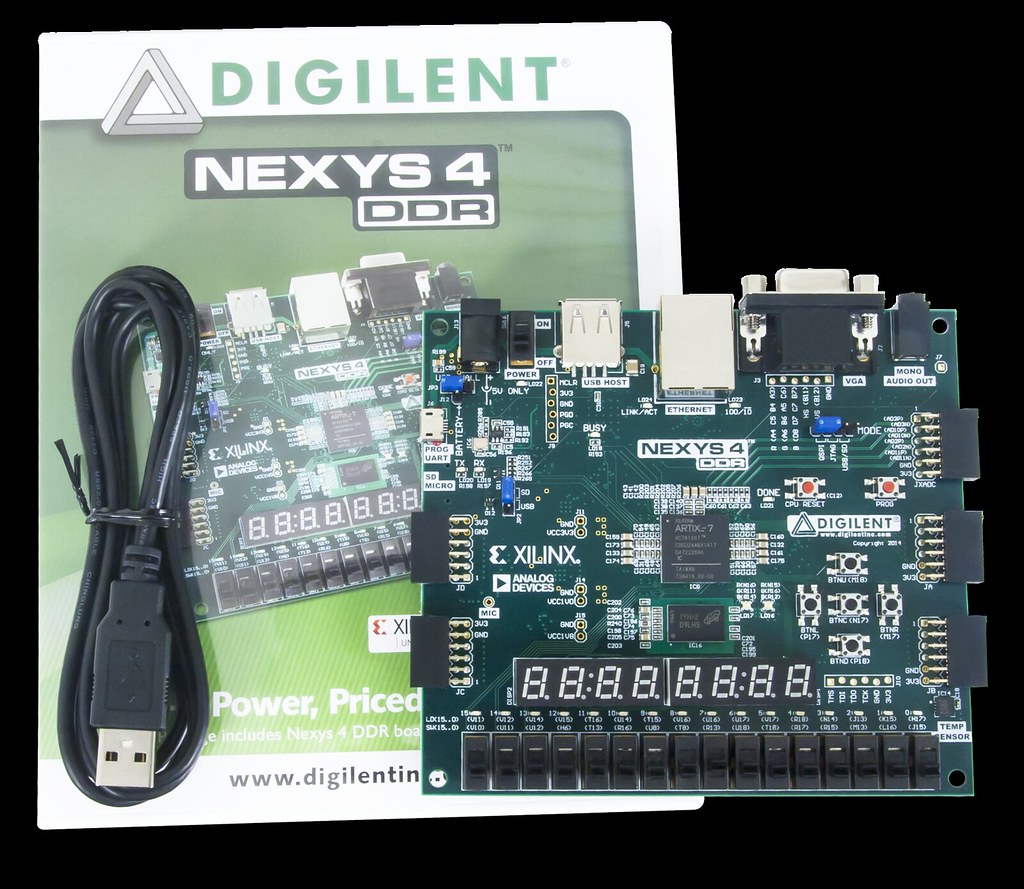
\includegraphics[width=0.4\linewidth]{images/img002_nexys4_ddr_board.jpg}
  \end{center}

  Documentatie:

  \begin{itemize}
    \item \url{https://reference.digilentinc.com/reference/programmable-logic/nexys-4-ddr/reference-manual}
    \item \url{https://reference.digilentinc.com/\_media/reference/programmable-logic/nexys-4-ddr/nexys4ddr\_rm.pdf}
  \end{itemize}
\end{minipage}

\begin{minipage}{\linewidth}
  \subsection{De Nexys A7}

  Dit is het bovenstaande Nexys4 DDR-bord, opnieuw uitgebracht onder een andere naam:

  \begin{center}
    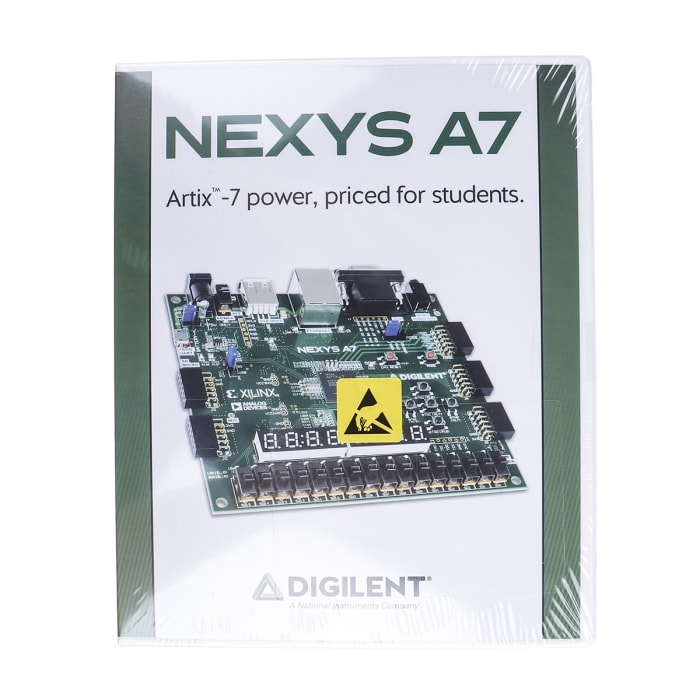
\includegraphics[width=0.4\linewidth]{images/img003_nexysA7_board.jpg}
  \end{center}

  Documentatie:

  \begin{itemize}
    \item \url{https://reference.digilentinc.com/reference/programmable-logic/nexys-a7/reference-manual}
    \item \url{https://reference.digilentinc.com/\_media/reference/programmable-logic/nexys-a7/nexys-a7\_rm.pdf}
  \end{itemize}
\end{minipage}

\newpage

\section{Stroom, jumpers, schakelaars en knoppen}

Deze foto van bovenaf toont de belangrijkste jumperposities op het Nexys4-bord:

  \begin{center}
    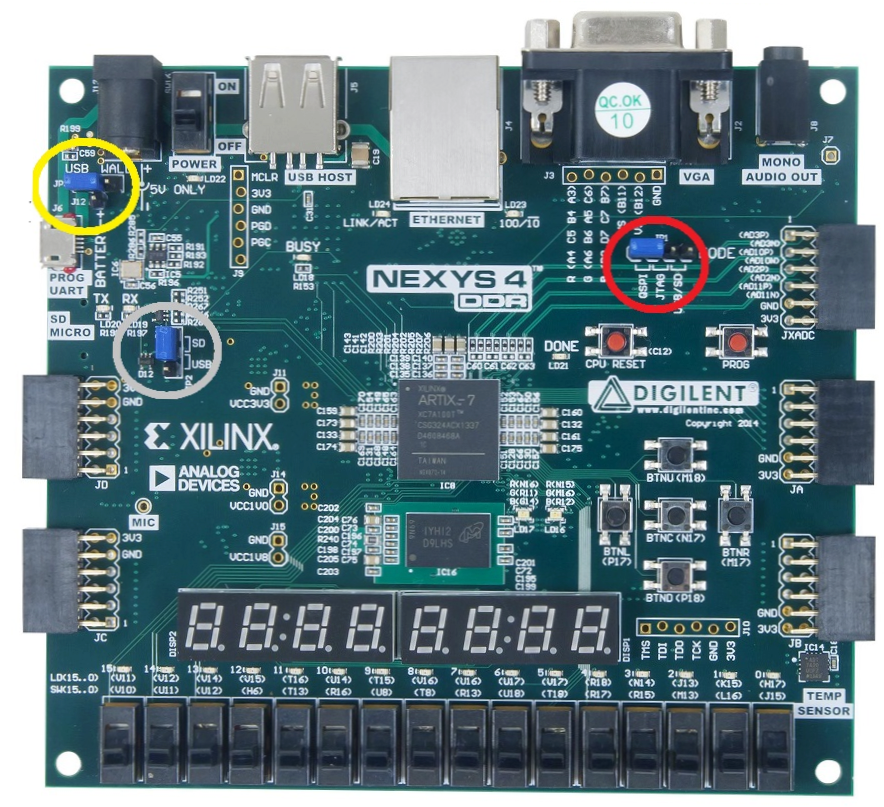
\includegraphics[width=0.9\linewidth]{images/nexys4_jumpers.png}
  \end{center}

De Nexys4-borden kunnen op twee manieren van stroom worden voorzien: via een externe voeding of via een standaard USB-poort.

\subsection{Micro-USB-voeding}

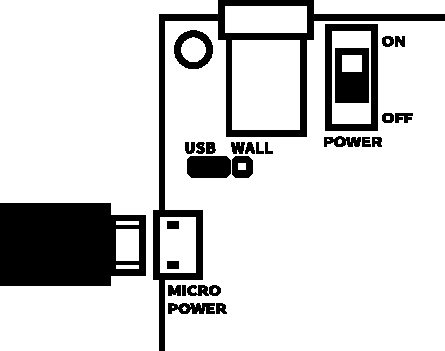
\includegraphics[width=5cm]{images/illustrations/nexys-micro-usb-power.pdf}

Sluit uw micro-USB-kabel aan op een USB-poort van een USB-lader of pc om stroom te leveren. Sluit het andere uiteinde aan op de micro-USB-connector van de Nexys4. Plaats de JP3-jumper op pennen 1 en 2 om USB-voeding te selecteren. Gebruik de schakelaar om de Nexys4 in te schakelen.

\subsection{Externe voeding}

\hspace*{1.7cm}
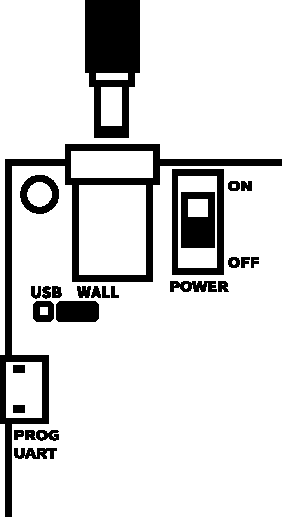
\includegraphics[width=3.2cm]{images/illustrations/nexys-power-supply.pdf}

De MEGA65-core kan veel stroom verbruiken en een standaard USB-poort kan in potentie te weinig vermogen leveren voor het Nexys4-bord. Het schrijven naar de SD-kaart kan met name vastlopen of vreemd gedrag vertonen. U wordt dan aangeraden een voeding van 5V te gebruiken.

Digilent verkoopt een voeding voor het Nexys4-bord en wij raden u aan deze te gebruiken om het risico op schade aan uw Nexys4-bord te vermijden. De gekozen voeding moet een center-positieve stekker met een binnendiameter van 2.1 mm hebben en 4.5VDC tot 5.5VDC leveren met een stroomsterkte van ten minste 1 ampère.

Sluit de voedingskabel aan op de voedingsaansluiting van de Nexys4. Plaats de JP3-jumper op pennen 2 en 3 om netvoeding te selecteren. Gebruik de schakelaar om de Nexys4 in te schakelen.

\subsection{Overige jumpers en schakelaars}

Voor uw eerste installatie raden wij u aan de volgende jumpers op uw Nexys4-bord in te stellen:

\begin{itemize}
  \item{JP1} - USB/SD  \item{JP2} - SD
\end{itemize}

\begin{center}
  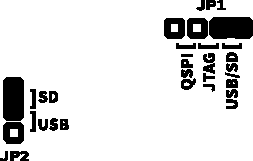
\includegraphics[width=3.2cm]{images/illustrations/nexys-jumpers.pdf}
\end{center}

Dit zorgt ervoor dat de bitstream-bestanden bij het opstarten vanaf uw SD-kaart geladen worden.

Op een later moment kunt u ervoor kiezen de bitstream vanaf de ingebouwde QSPI-flash te laden. In dat geval kunt u de instelling van de JP1-jumper aanpassen naar de QSPI-positie.

% XXX - Image of board highlighting the jumpers

Alle 16 schakelaars aan de onderkant van het bord moeten op de uit-positie staan.


\subsection{Aansluitingen en randapparatuur}

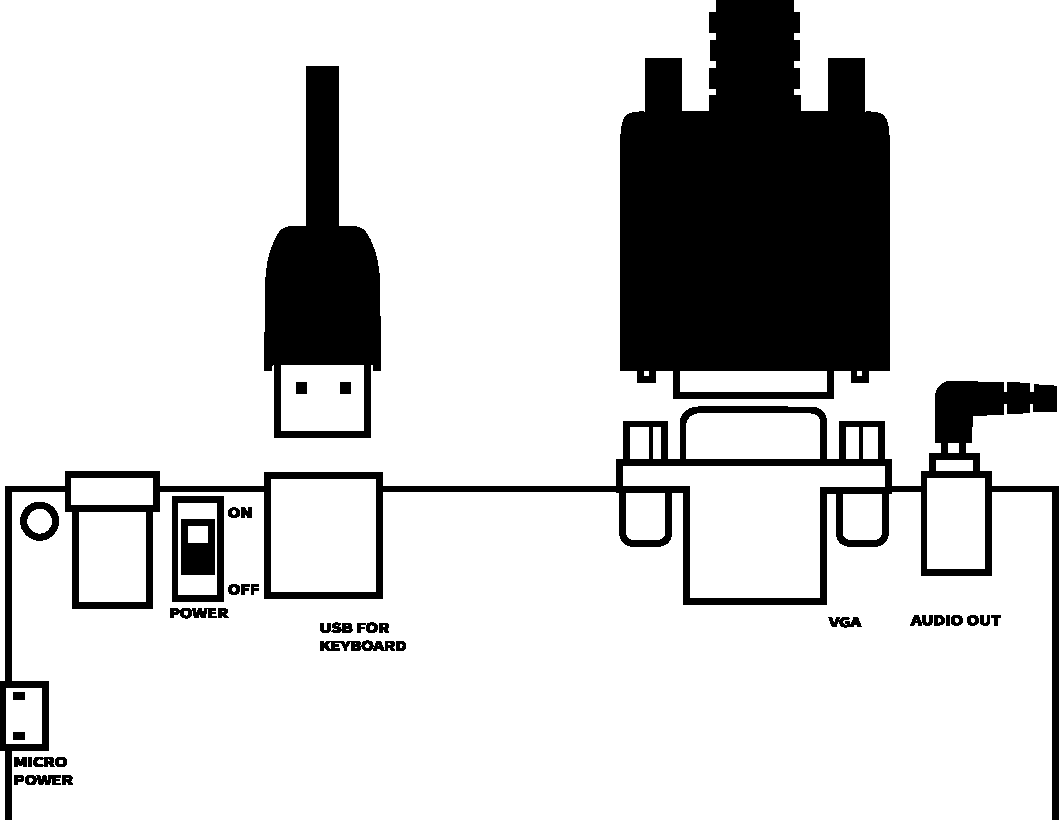
\includegraphics[width=\linewidth]{images/illustrations/nexys-connectors.pdf}

Aan de USB-poort kan een USB-toetsenbord worden aangesloten. Alleen een toetsenbord zonder USB-hub werkt met het Nexys4-bord. Over het algemeen werken zeer goedkope toetsenborden, terwijl duurdere toetsenborden vaak een USB-hub bevatten en niet werken. Het zou kunnen voorkomen dat u meerdere toetsenborden moet proberen voordat u er een vindt die werkt.

Aan de VGA-poort kan een VGA-beeldscherm worden aangesloten.

De mono-audio-uitgang kan worden aangesloten op de line-in van een versterker.


\subsection{Communicatie met uw pc}

Er kunnen situaties zijn waarin u vanaf uw pc met het Nexys4-bord wilt communiceren, bijvoorbeeld om de volgende activiteiten uit te voeren:

\begin{itemize}
  \item Het QSPI-flashgeheugen flashen via Vivado  \item Bitstream-bestanden rechtstreeks vanaf uw pc uploaden (via het m65-hulpprogramma)  \item Hulpprogramma's gebruiken zoals M65Connect, m65, mega65\_ftp, m65dbg, enz.
\end{itemize}

In zulke gevallen moet u de micro-USB-kabel op uw pc aansluiten.

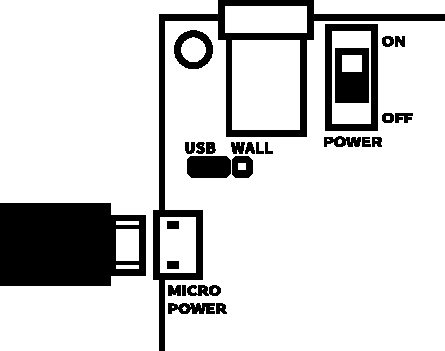
\includegraphics[width=5cm]{images/illustrations/nexys-micro-usb-power.pdf}

\subsection{Knoppen op het bord}

\begin{center}
  
\includegraphics[width=3.2cm]{images/illustrations/nexys-reset-buttons.pdf}
\end{center}

De ``CPU RESET''-toets reset de MEGA65 wanneer u deze indrukt, terwijl de ``PROG''-toets de FPGA zelf de MEGA65-core laat herladen. Het belangrijkste verschil tussen de twee is dat CPU RESET sneller is en de inhoud van het geheugen niet wist, terwijl de FPGA-knop langzamer is en de inhoud van het geheugen wel reset.

\begin{center}
  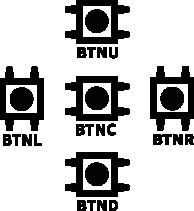
\includegraphics[width=3.2cm]{images/illustrations/nexys-five-buttons.pdf}
\end{center}

Twee van de vijf toetsen in de kruisopstelling kunnen eveneens worden gebruikt: BTND gedraagt zich alsof u \widekey{RESTORE} heeft ingedrukt, terwijl BTNC een interrupt activeert, alsof de IRQ-lijn naar massa is getrokken.

\section{Toetsenbord}

De toetsenbordindeling is positioneel en niet logisch. Dit betekent dat toetsen die zich in dezelfde positie bevinden als de toetsen op een C65-toetsenbord een vergelijkbare functie hebben. Deze relatie gaat ervan uit dat uw USB-toetsenbord een Amerikaanse toetsenbordindeling gebruikt.

Om u te helpen bij het vinden van de toetstoewijzingen van de diverse MEGA65-toetsen, beschikt de MEGA65 over een ingebouwde virtuele toetsenbordtest. Deze is op twee manieren te bereiken.

De eenvoudigste manier is om \specialkey{ALT} ingedrukt te houden terwijl u de Nexys4 inschakelt, of de Nexys4 reset met de ``PROG''-toets. Het configuratiemenu wordt weergegeven en door op 3 te drukken, verschijnt het virtuele toetsenbord op een zwarte achtergrond.

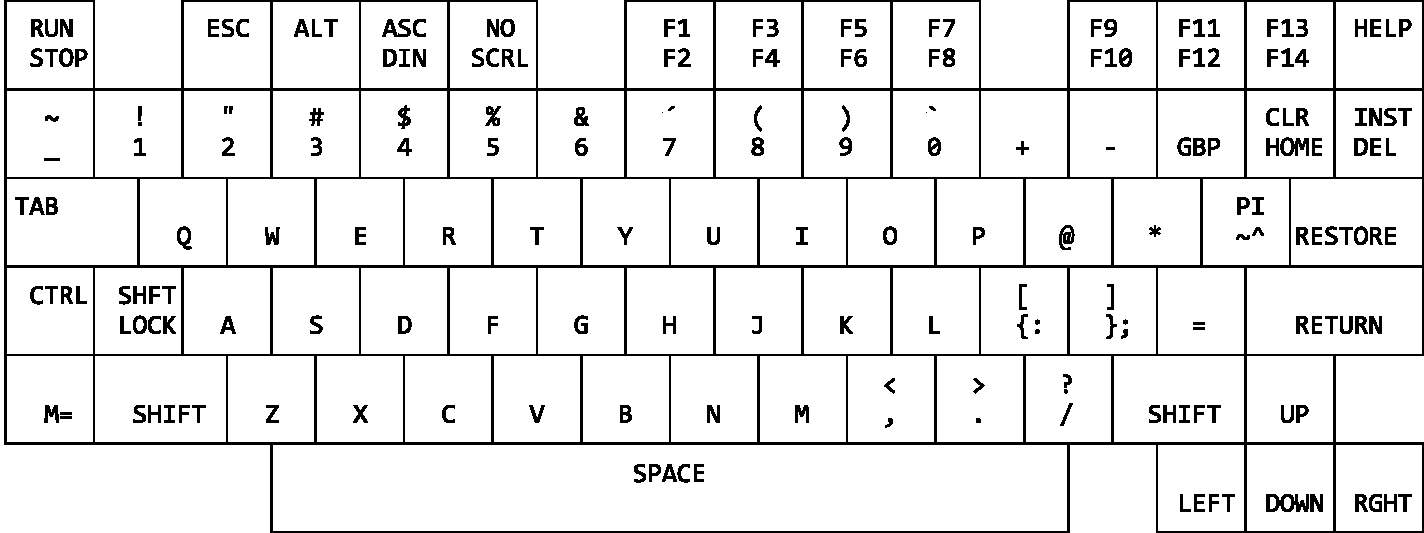
\includegraphics[width=\linewidth]{images/illustrations/virtual-keyboard.pdf}

Wanneer u een toets op het USB-toetsenbord indrukt, wordt de betreffende toets op het virtuele toetsenbord gemarkeerd weergegeven om u te helpen bij het herkennen van de toetstoewijzing.

De andere manier om het virtuele toetsenbord te bereiken is vanuit de MEGA65 zelf. Houd \megasymbolkey ingedrukt en druk op \specialkey{TAB} om de Matrix Mode Debugger te openen. Voer vervolgens het volgende in:

\screentextwide{s ffd3615 ff}

Dit opent een halfdoorzichtig virtueel toetsenbord aan de bovenkant van het scherm. Als alternatief:

\screentextwide{s ffd3615 ff ff}

Dit opent een halfdoorzichtig virtueel toetsenbord in het midden van het scherm.

Houd \megasymbolkey ingedrukt en druk op \specialkey{TAB} om de Matrix Mode Debugger te verlaten en terug te keren naar de MEGA65.

\subsection{Enkele toetstoewijzingen met een USB-toetsenbord}

\widekey{RESTORE} is toegewezen aan de Page Up-toets.

\specialkey{RUN\\STOP} is toegewezen aan \specialkey{ESC}.

\newpage

\section{MicroSDHC-kaart voorbereiden}

De MEGA65 vereist een SDHC-kaart met een capaciteit van 4 GB tot 64 GB. Sommige SDXC-kaarten kunnen werken, maar dit wordt niet officieel ondersteund.

De voorbereidingsstappen voor de SD-kaart van het Nexys4-bord komen grotendeels overeen met de stappen die nodig zijn voor echte MEGA65-hardware. Het is dan ook de moeite waard om een kijkje te nemen in
\ifdefined\printmanual
het {\bf grote Mega65-boek}
\else
\bookvref{cha:configuringyourmega}
\fi
als u ooit meer details nodig heeft.

In dit onderdeel bespreken we de specifieke stappen uitgebreider en beperken we ons tot een beknopte behandeling van de gemeenschappelijke stappen.

Een verschil tussen het Nexys-bord en de echte MEGA65-hardware is dat laatstgenoemde standaard een bitstream/core bevat waarmee u uw SD-kaart in de specifieke indeling kunt formateren die door de MEGA65 wordt vereist.

Voor eigenaren van het Nexys4-bord is er echter geen standaard bitstream; raadpleeg daarom het {\bf grote Mega65-boek} voor meer informatie over waar u de juiste bestanden ``nexys4.bit of ``nexys4ddr-widget.bit voor uw apparaat kunt downloaden.

\subsection{Voorbereidingsstappen}

De stappen zijn:

\begin{itemize}
  \item{Formateer de SD-kaart} op een handige computer met het FAT32-bestandssysteem. De MEGA65- en Nexys4-borden ondersteunen geen andere bestandssystemen, met name niet het exFAT-bestandssysteem.\item{Kopieer} uw bitstream-bestand (met een bestandsnaam die eindigt op ``.bit'') naar de SD-kaart.\item{Plaats} de SD-kaart in de SD-kaartsleuf aan de onderkant van het Nexys4-bord.\item{Schakel} het Nexys4-bord in.\item{Open het hulpprogrammamenu} door \specialkey{ALT} ingedrukt te houden op het USB-toetsenbord dat op het Nexys4-bord is aangesloten wanneer het MEGA65-startscherm wordt weergegeven.\item{Open het FDISK/FORMAT-hulpprogramma} door op 2 te drukken wanneer de optie verschijnt op het MEGA65-opstartscherm.\item{Volg de aanwijzingen} in het FDISK/FORMAT-programma om de SD-kaart opnieuw te formatteren voor gebruik door de MEGA65. \\
  \\
  Het FDISK-hulpprogramma maakt twee partities op uw SD-kaart aan en formatteert deze.
  \begin{itemize}
    \item De ene is type \$41 = MEGA65-systeempartitie, waar de opslagslots, configuratiegegevens en andere bestanden staan. \\  (Deze partitie is onzichtbaar op bijvoorbeeld Windows-pc's).    \item De andere partitie met type \$0C = VFAT32, waar KERNAL, ondersteuningsbestanden, spellen enzovoort later naartoe worden gekopieerd. \\  (Deze partitie is zichtbaar op bijvoorbeeld Windows-pc's).
  \end{itemize}
\item{Zodra het formatteren is voltooid}, schakelt u het Nexys4-bord uit en verwijdert u de microSDHC-kaart uit het Nexys-bord en plaatst u deze terug in uw pc\item{Kopieer} deze keer de volgende items naar de SD-kaart:
  \begin{itemize}
    \item Het bitstream-bestand    \item De uitgepakte bestanden uit het ``\textbf{SD essentials.rar}''-of het ``\textbf{SD essentialsNoROM.rar}''-bestand dat u van de MEGA65-filehost hebt gedownload.    \item{Als u uw eigen voorkeurs-ROM-bestand hebt} (bijvoorbeeld ``\textbf{911001.BIN}''), kopieer dit ook naar de SD-kaart en hernoem het naar ``\textbf{MEGA65.ROM}'' (hoofdletters zijn verplicht).    \item{Eventuele .D81-schijfimage-bestanden} waarvan u gebruik wilt maken.
      \begin{itemize}
        \item Let op: wanneer een bestand met de naam MEGA65.D81 aan de SD-kaart wordt toegevoegd, wordt dit automatisch gemonteerd bij het opstarten.        \item Zorg ervoor dat alle .D81-bestanden namen hebben die voldoen aan de oude DOS 8.3-tekenlimiet en in hoofdletters zijn geschreven. Deze beperking wordt in een toekomstige versie verwijderd.
      \end{itemize}
  \end{itemize}
\item{Verwijder de SD-kaart} en plaats deze terug in uw Nexys4-bord.\item{Schakel het Nexys4-bord} weer in. De MEGA65 zou binnen 15 seconden moeten opstarten.\item"Bij de eerste opstart bevindt u zich op het onboarding-scherm, waarvan meer details te vinden zijn in
\ifdefined\printmanual
het {\bf grote Mega65-boek}
\else
\bookvref{cha:configuringyourmega}
\fi
.

\end{itemize}

Gefeliciteerd. Uw MEGA65 is ingesteld en gereed voor gebruik.

Houd er rekening mee dat bij de bovenstaande methode het bitstream-bestand naar de SD-kaart wordt gekopieerd, waardoor de Nexys-FPGA de bitstream bij elke opstartcyclus laadt; het opstarten duurt dan ongeveer 13 seconden. De bitstream kunt u ook met Vivado-software naar het QSPI-flashgeheugen flitsen; de opstarttijd verkort u daarmee tot 0.3 seconden.

Voor meer gedetailleerde informatie over het voorbereiden en configureren van uw MEGA65 verwijzen wij u naar
\ifdefined\printmanual
het {\bf grote Mega65-boek}
\else
\bookvref{cha:configuringyourmega}
\fi
hoofdstuk.

\section{De bitstream laden vanuit QSPI}

Hoewel het laden van de bitstream vanaf de SD-kaart de aanbevolen (en veelbewandelde) route is die dit document heeft gekozen, hebben de laatste tijd meer Nexys4-gebruikers de alternatieve weg verkend om de bitstream vanuit het QSPI-flashgeheugen te laden. Enkele mogelijke redenen hiervoor zijn:

\begin{itemize}
  \item Snellere opstarttijden (0,3 seconden versus 13 seconden)  \item Sommige gebruikers waren geïnteresseerd in de mogelijkheid om meerdere cores op hun QSPI te flitsen (via stappen die beschreven staan in de
\ifdefined\printmanual
het {\bf grote Mega65-boek}
\else
\bookvref{cha:cores}
\fi
		Hoofdstuk)  \item Sommige gebruikers hebben last gehad van hardnekkige problemen met de route via de SD-kaart, zoals:
    \begin{itemize}
      \item Het systeem kan niet opnieuw opstarten vanaf het onboarding-scherm      \item Het systeem kan niet opnieuw opstarten vanuit het freeze-menu na het wisselen tussen PAL/NTSC
    \end{itemize}
\end{itemize}

Indien dit in de toekomst een populairdere route blijkt te zijn, kunnen wij onze documentatie hierop aanpassen. Hier volgen enkele stappen in het kort.

\subsection{Voorbereidingsstappen}

Als u deze route wilt proberen, moet u de JP1-jumperinstelling aanpassen om QSPI te gebruiken en vervolgens de stappen volgen in het hoofdstuk \nameref{cha:fpgacpldflashing} met betrekking tot \nameref{sec:installvivado} en \nameref{sec:mainfpgaflashing}.

Houd er rekening mee dat de installatie van Vivado een langdurig proces is (zowel wat betreft de downloadtijd als de installatietijd).

Nadat u Slot0 van uw QSPI-chip hebt geflitst via Vivado, kunt u de stappen volgen die beschreven staan in
\ifdefined\printmanual
het {\bf grote Mega65-boek}
\else
\bookvref{cha:configuringyourmega}
\fi
voor de aangepaste SD-kaartformattering, het installeren van ROM- en ondersteuningsbestanden en de onboarding.

\section{Widget-bord}

Als u een Nexys-bord bezit (alle modellen), vindt u het wellicht interessant om een widget-bord aan uw Nexys-apparaat toe te voegen, zodat u verbinding kunt maken met:

\begin{itemize}
  \item{een originele C64- of C65-toetsenbord}
  \item{2 DB-9-joysticks}
  \item{Paddles of een 1351-muis}
  \item{Cartridges (werken nog niet)}
\end{itemize}

Het widget-bord wordt via de PMOD-connectoren met uw Nexys-bord verbonden.

Momenteel is het alleen verkrijgbaar als onbewerkte printplaat (zonder componenten), hier aan te schaffen:

\begin{itemize}
  \item \url{https://oshpark.com/shared\_projects/Y37xg9N7}
\end{itemize}

De firmware, de printplaatdiagrammen, het schema en de stuklijst zijn in het volgende GitHub-project te vinden:

\begin{itemize}
  \item \url{https://github.com/sy2002/DM65PIC}
\end{itemize}

U moet de onderdelen uit de stuklijst apart aanschaffen en de componenten zelf op het bord monteren.

Dit forum64.de-thread kan voor u van belang zijn wanneer u de ervaringen van anderen die dit proces hebben doorlopen wilt lezen of wanneer u zelf vragen heeft:

\begin{itemize}
  \item \url{https://www.forum64.de/index.php?thread/90465-mega-65-ports-add-on-card-still-available-if-where}
\end{itemize}

De printplaatbestanden (c65Keyb.brd) en schematische bestanden (c65Keyb.sch) bevinden zich in de map ``eagle/' van het DM65PIC-project en kunnen worden bekeken met het gratis programma AutoDesk Eagle, hier beschikbaar:

\begin{itemize}
  \item \url{https://www.autodesk.com/products/eagle/free-download}
\end{itemize}

Hier volgen enkele foto's van het widget-bord in gebruik:
  \begin{center}
    \includegraphics[width=0.9\linewidth]{images/widget-board-martin.png}
  \end{center}
  \begin{center}
    \includegraphics[width=0.9\linewidth]{images/widget-board-deft1.png}
  \end{center}
  \begin{center}
    \includegraphics[width=0.9\linewidth]{images/widget-board-deft2.png}
  \end{center}

Voor het gemak zijn de printplaat- en schema's van het widget-bord eveneens opgenomen in \bookvref{sec:nexyswidgetschematics}.

Enkele aanvullende achtergrondnotities over het bord:

\begin{itemize}
  \item{Het widget-bord is oorspronkelijk bedoeld om in een C65-behuizing te passen}
  \item{De uitbreidingspoort is niet bruikbaar en er moet een stuk worden weggezaagd voor de C64-behuizing}
  \item{Het zou redelijk zijn het bord aan te passen voor gebruik in een C64-behuizing (wat zeker het meest voorkomende gebruik zal zijn)}
\end{itemize}

\section{PMOD-naar-joystick-adapter}

Als alternatief (en goedkoper) voor wie alleen een DB9-joystick-poort via de PMOD-connectoren wil toevoegen, heeft een community-lid, TheChief, een manier bedacht om dat te doen. Meer informatie is te vinden in het volgende Discord-thread:

\begin{itemize}
  \item \url{https://discord.com/channels/719326990221574164/903079038015389716/929369283119685643}
\end{itemize}

  \begin{center}
    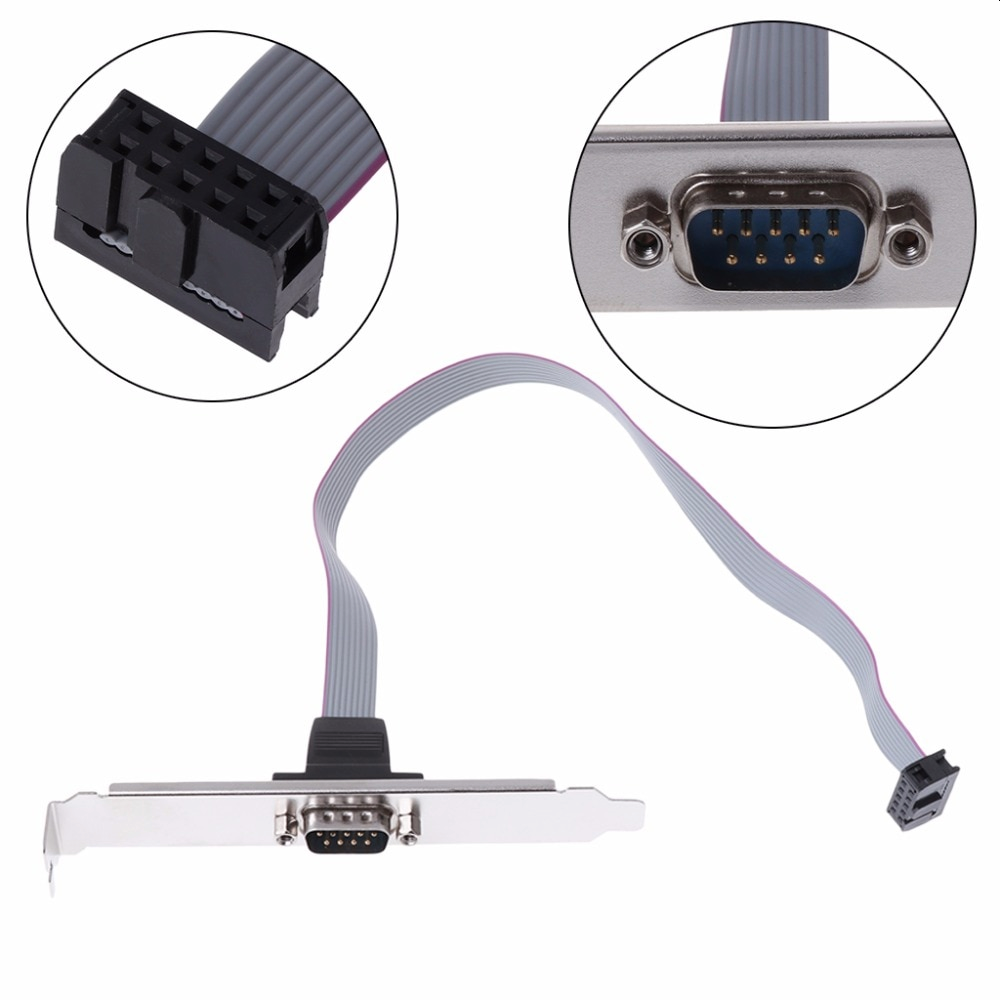
\includegraphics[width=0.9\linewidth]{images/joystick-pmod-thechief.png}
  \end{center}

\begin{minipage}{\linewidth}
\begin{center}
  \begin{longtable}{|L{3cm}|L{3cm}|p{3cm}|}
    \hline
    {\textbf{Joystick-actie}} & {\textbf{PMOD-JA-aansluitingen}} & {\textbf{DB9-aansluitingen}} \\
    \hline
    {Vuur} & {jahi(9)} & {pin 6} \\
    \hline
    {Omhoog} & {jalo(1)} & {pin 1} \\
    \hline
    {Links} & {jalo(2)} & {pin 3} \\
    \hline
    {Omlaag} & {jahi(7)} & {pin 2} \\
    \hline
    {Rechts} & {jahi(8)} & {pin 4} \\
    \hline
  \end{longtable}
\end{center}
\end{minipage}


\section{Handige tips}

Hier volgen enkele handige tips om vertrouwd te raken met de MEGA65:

\begin{itemize}

\item{Druk op \& houd \megasymbolkey (of de Commodore-toets als u een Commodore 64- of 65-toetsenbord gebruikt) ingedrukt tijdens het opstarten om in C64-modus op te starten in plaats van C65-modus.}
 \item{Druk op \& houd \specialkey{RUN\\STOP} ingedrukt tijdens het opstarten om de machine-taalmonitor te openen in plaats van BASIC te starten.}
\item{Druk op \widekey{RESTORE} en houd deze ongeveer een halve tot een seconde ingedrukt om het MEGA65 Freeze-menu te openen. Dit menu biedt handige hulpmiddelen om de processorsnelheid te wijzigen, te wisselen tussen PAL \& NTSC-videomodus, audio-instellingen aan te passen, freeze-states te beheren en D81-schijfimages te selecteren. U kunt bovendien het geheugen van het bevroren programma inspecteren en bewerken, en nog veel meer. Dit menu is in vele opzichten het hart van de MEGA65 en is het ontdekken zeker waard.}
\item{Typ \screentext{POKE0,65} in C64-modus om de processor op volle snelheid (40 MHz) te zetten. Sommige software gedraagt zich in deze modus onjuist, terwijl andere software juist sneller werkt.}
\item{Typ \screentext{POKE0,64} in C64-modus om de processor op 1 MHz te zetten.}
\item{Typ \screentext{SYS58552} in C64-modus om naar C65-modus te schakelen.}
\item{Typ \screentext{GO64} in C65-modus en bevestig door \screentext{Y} in te drukken om naar C64-modus te schakelen, hetzelfde als op een C128.}
\item{De C65-ROM maakt apparaat 8 tot standaard, zodat u het \textbf{,8} aan het einde van LOAD- en SAVE-commando's normaal gesproken kunt weglaten.}
\item{Het indrukken van \specialkey{SHIFT} + \specialkey{RUN\\STOP} in de C64- of C65-modus probeert van schijf op te starten.}
\end{itemize}

Veel plezier! Veel plezier! Er is jarenlang met liefde aan de MEGA65 gewerkt voor uw plezier. Wij hopen dat u er net zoveel plezier aan beleeft als wij bij het maken hebben gehad!

Het MEGA Museum of Electronic Games \& Art verwelkomt uw feedback, suggesties en bijdragen aan dit open-source-project voor het bewaren van digitaal erfgoed.


\part{PLATFORMONAFHANKELIJKE ONTWIKKELHULPMIDDELEN}

\chapter{Emulators}

Op het moment van schrijven is er slechts één emulator voor de MEGA65,\ \stw{xmega65}; de Xemu-emulatorsuite van LGB. De LGB-ontwikkelaars werken hard om bij te blijven met de ontwikkeling van de MEGA65; niettemin is sommige MEGA65-emulatie mogelijk niet nauwkeurig, maar zou deze voldoende moeten zijn voor softwareontwikkeling op de MEGA65.

% Should there be a link to the LGB suite?

Test software tijdens de ontwikkeling regelmatig op echte hardware, zoals een MEGA65 of een FPGA-board dat een MEGA65-core kan uitvoeren.

Download de broncode van de MEGA65-emulator van \url{https://github.com/lgblgblgb/xemu}.

Download voorgecompileerde versies van \url{https://github.lgb.hu/xemu/}. Installers
zijn beschikbaar voor macOS, Windows en Linux.

Een live ISO-image met de emulator, documentatie en andere hulpprogramma's is beschikbaar via
Forum64.de
op \url{https://www.forum64.de/index.php?thread/104698-xemu-live-system-iso-file/\&postID=1549927\#post1549936}.
Indien u deze wilt gebruiken, vindt u de instructies op bladzijde \pageref{sec:live-iso-image}.

\section{De Xmega65-emulator gebruiken}
\index{emulator}

\subsection{Het toetsenbord}
\label{sec:xemu-keyboard}
\index{toetsenbord}

De MEGA65-toetsenbordindeling is gebaseerd op de Commodore 65, wat afwijkt van een modern pc-toetsenbord. In de meeste gevallen herkent de Xmega65-emulator pc-toetsen als hun equivalente MEGA65-toetsen, zoals letters, cijfers en veelgebruikte modificatietoetsen zoals \specialkey{Shift}. Xmega65 gaat uit van een Amerikaanse (VS-)indeling.

Sommige toetsen komen alleen op het MEGA65-toetsenbord voor en hebben geen pc-equivalenten. Xmega65
gebruikt de pc-toetsen \specialkey{Insert}, \specialkey{Delete}, \specialkey{Home},
\specialkey{End}, \specialkey{Page Up} en \specialkey{Page Down} voor
\megakey{+}, \megakey{\pounds}, \specialkey{CLR\\HOME}, \specialkey{RUN\\STOP},
\specialkey{HELP} en \widekey{RESTORE}, respectievelijk.

\begin{center}
  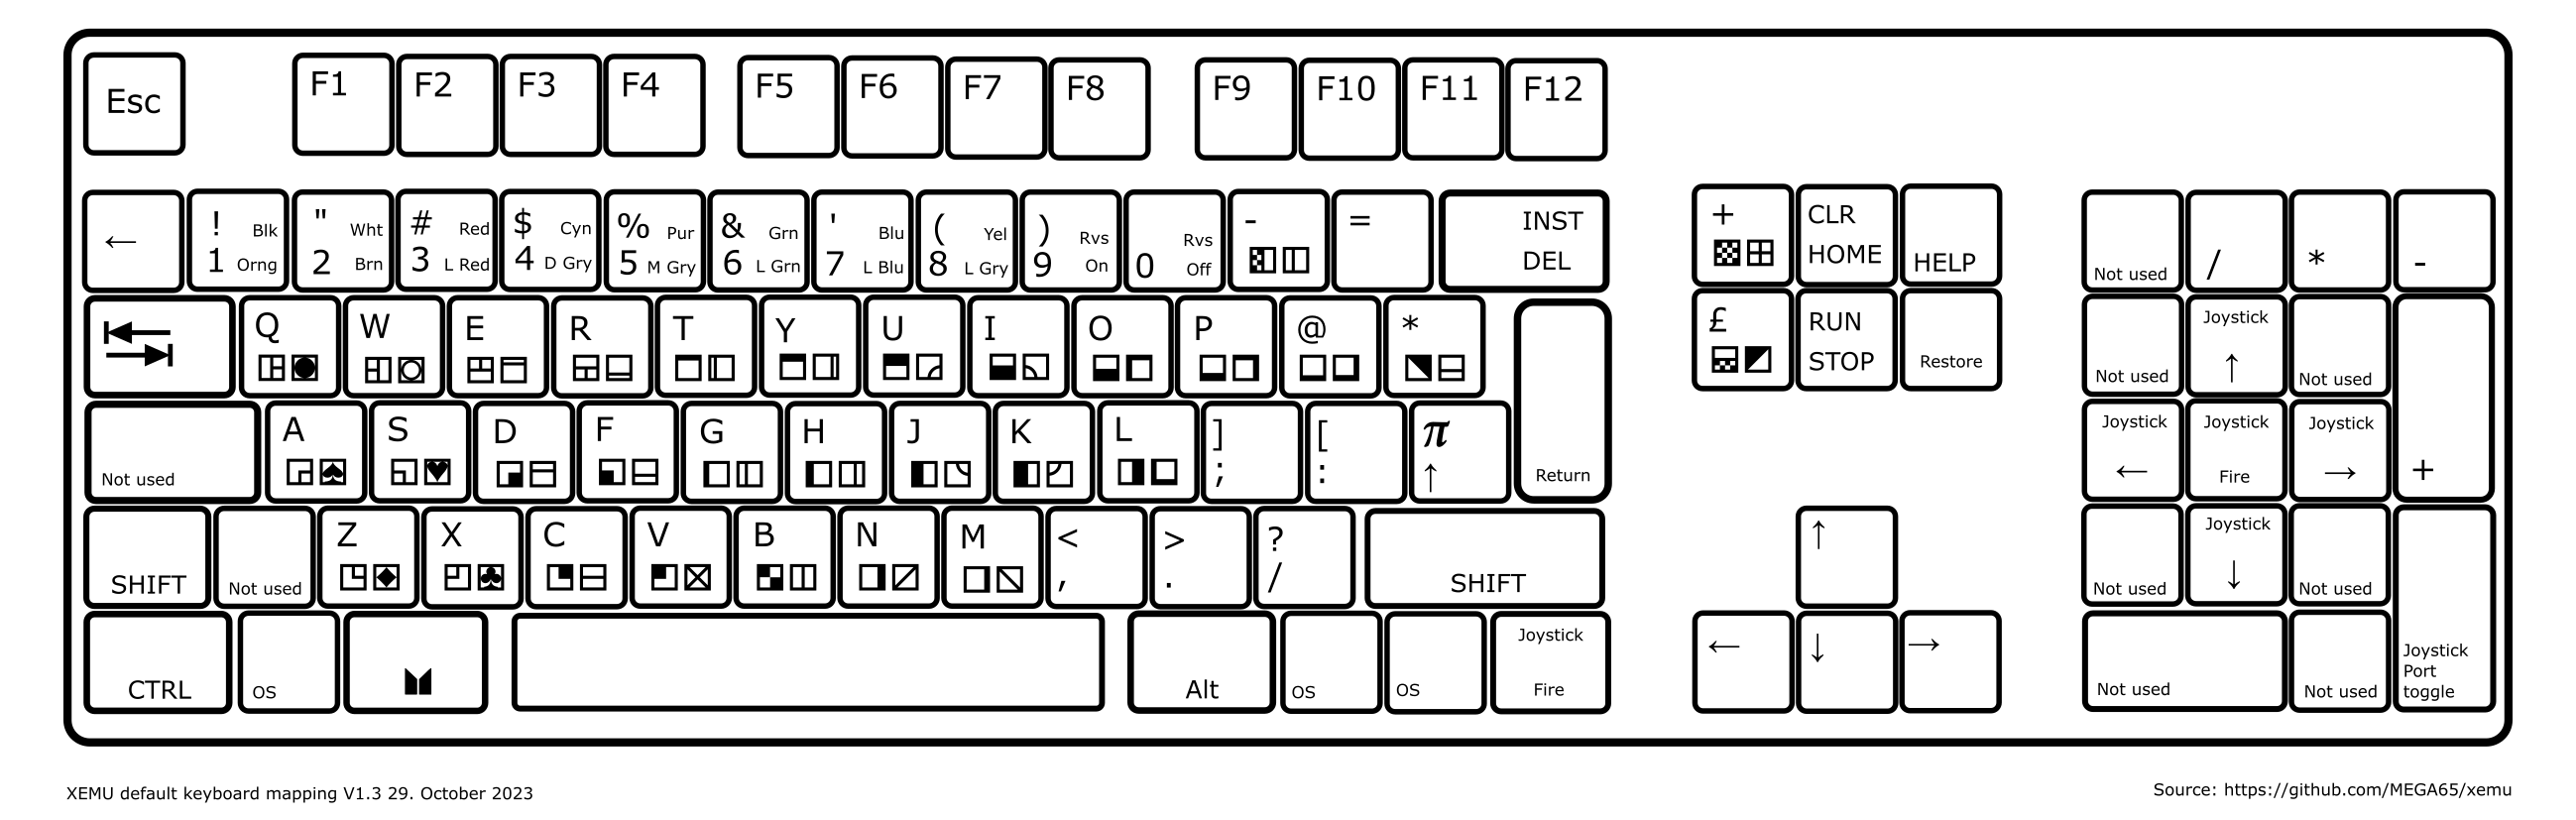
\includegraphics[width=\linewidth]{images/xemu-extended-keyboard.png}
\end{center}

Op de meeste pc-toetsenborden staan \specialkey{RUN\\STOP} en \widekey{RESTORE} naast elkaar,
zodat deze toetscombinatie eenvoudig is in te voeren.

Deze afbeelding toont de PETSCII-glyphen zoals ze op een MEGA65-toetsenbord verschijnen, met de
\megasymbolkey-glyphe links en de \specialkey{Shift}-glyphe rechts. Merk op
dat op een pc-toetsenbord de toets voor \megasymbolkey rechts van de
\specialkey{Shift} staat.

Xemu biedt twee joysticks (een per keer) op het numerieke toetsenbord.
\specialkey{Enter} op het numerieke toetsenbord wordt gebruikt om bij herhaaldelijk drukken poorten 1 en 2 in en uit te schakelen.

Wees u ervan bewust dat de emulator standaard \megakey{F9} \megakey{F10}
\megakey{F11} als eigen sneltoetsen heeft gedefinieerd. Als u deze toetsen wilt gebruiken met de
geëmulieerde MEGA65, moet u de toetsenbordindeling aanpassen. De bestanden staan in de
map met de Xemu-instellingen zoals uitgelegd op bladzijde
\pageref{sec:sdcard-settings-location}. Dit doet u door
\stw{keymap-default.cfg} te kopiëren naar \stw{keymap.cfg} en vervolgens de volgende regels te verwijderen:

\begin{tcolorbox}[colback=black,coltext=white]
\verbatimfont{\codefont}
\begin{verbatim}
XEMU-EXIT F9
XEMU-FULLSCREEN F11
\end{verbatim}
\end{tcolorbox}

en te wijzigen in:

\begin{tcolorbox}[colback=black,coltext=white]
\verbatimfont{\codefont}
\begin{verbatim}
F9 Unknown
F11 Unknown
\end{verbatim}
\end{tcolorbox}

naar:

\begin{tcolorbox}[colback=black,coltext=white]
\verbatimfont{\codefont}
\begin{verbatim}
F9 F9
F11 F11
\end{verbatim}
\end{tcolorbox}

Nadat deze toetsen opnieuw zijn toegewezen, zijn de functies voor volledig scherm en afsluiten nog steeds beschikbaar via
het menu. Klik met rechts (of Ctrl-klik) ergens in het venster om dit te openen.

\subsection{Problemen met starten op Apple MacOS}

Als het bericht \stw{macOS cannot verify that this app is free from malware} verschijnt,
gebruik dan de volgende procedure wanneer u de app voor de eerste keer opent:\index{Apple}
\index{macOS}

\begin{itemize}
  \item Open Finder op uw Mac.
  \item Ctrl-klik (of rechtsklik) op het Xmega65-app-pictogram.
  \item Selecteer in het contextmenu \stw{Open}.
  \item Het bericht verschijnt opnieuw, maar deze keer is er een knop \stw{Open}.
        Klik op \stw{Open}. U hoeft deze procedure slechts de eerste keer uit te voeren.
		Vanaf nu kunt u de app normaal openen.
\end{itemize}

\subsection{Instellingen bijwerken}
\label{sec:sdcard-settings-location}
\index{SD-kaart}

U kunt het Xemu-instellingsbestand bewerken om de toetsenbordindeling aan te passen of een
reservekopie van het SD-kaart-imagebestand te maken. Open vanuit Xemu het menu om deze bestanden te openen: selecteer
menu, selecteer \stw{Debug / Advanced} en vervolgens \stw{Browse system folder}. Bewerk de
bestanden \stw{keymap-default.cfg} en \stw{mega65-default.cfg} met een teksteditor.
Voor specifieke instructies over het wijzigen van \stw{keymap-default.cfg} verwijzen we naar
bladzijde \pageref{sec:xemu-keyboard}.

\begin{center}
  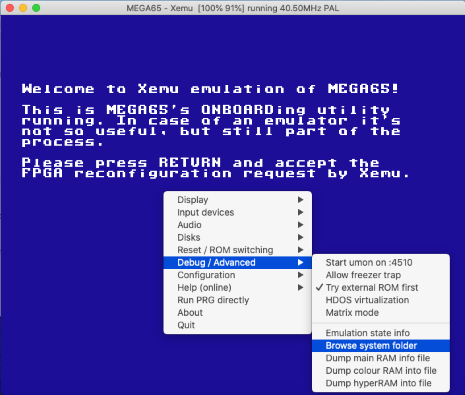
\includegraphics[width=0.5\linewidth]{images/xemusettings.png}
\end{center}

De locatie van de Xemu-systeemmap verschilt per besturingssysteem:

\begin{itemize}
    \item Windows (kan in de adresbalk van de verkenner worden gekopieerd):
    \stw{\%appdata\%$\textbackslash$xemu-lgb$\textbackslash$mega65}
    \item Linux:
    \stw{$\textasciitilde$/.xemu-lgb/}
    \item Macintosh:
    \stw{$\textasciitilde$/Library/Application$\textbackslash$ Support/xemu-lgb/mega65/}
\end{itemize}

\section{De Live ISO-image gebruiken}
\label{sec:live-iso-image}

De Live ISO-image is het product van een vrijwillige gemeenschap; niet van het MEGA65-team. We nemen deze op voor uw gemak.

\subsection{Een opstartbare USB-stick of DVD maken}

Er zijn veel manieren om een live ISO-image te maken. De methode die u kiest hangt af van uw besturingssysteem en of u deze op een USB-station wilt installeren of op een DVD wilt branden. Het branden op een DVD is eenvoudig, ervan uitgaande dat u een computer met een DVD-brander hebt. Als u een sneller opstartbaar USB-station wilt maken, probeert u een van de onderstaande methoden:

Als u Windows gebruikt, overweeg dan een hulpprogramma zoals \url{http://www.isotousb.com/}.

Op Linux kunt u de instructies op \url{https://fossbytes.com/create-bootable-usb-media-from-iso-ubuntu/} volgen.

Voor Apple Macs zijn de instructies op
\url{https://ubuntu.com/tutorials/create-a-usb-stick-on-macos#1-overview} beschikbaar.

Vergelijkbare instructies zijn beschikbaar voor andere populaire computers, zoals Amiga's (\url{https://forum.hyperion-entertainment.com/viewtopic.php?t=3857}) of Sun UltraSPARC-werkstations (\url{https://forums.servethehome.com/index.php?threads/how-to-create-a-bootable-solaris-11-usb.1998/}).

Tot slot is de populaire, eenvoudig te gebruiken en gratis cross-platform belanaEtcher beschikbaar op \url{https://www.balena.io/etcher/}.

\subsection{Aan de slag}

Om potentiële auteursrechtelijke kwesties te vermijden, bevat de opstartbare ISO-image geen propriëtaire ROM's voor de MEGA65, zoals oude C65-ROM's. Het bevat wel een vervangende open-source-ROM van ons OpenROMs-project.\index{OpenROMs} Deze ROM start op in een BASIC 2-omgeving waarmee u veel C64-programma's kunt laden en uitvoeren, zoals te zien is in de onderstaande afbeelding:

\screenshotwrap{images/liveiso-openrom.png}

Als u een C65-ROM met BASIC 10 wilt gebruiken, download het juiste ROM-bestand en plaats het op een andere USB-stick met de naam \stw{MEGA65.ROM}. Bij het opstarten zal de MEGA65 vragen of een ROM is gedownload; zoals te zien is in de onderstaande afbeelding:

\screenshotwrap{images/liveiso-rom-usb-prompt.png}

Als de Live ISO geen ROM kan vinden, zal het u vragen om een ROM te downloaden; zoals hieronder te zien is:

\screenshotwrap{images/liveiso-rom-download-prompt.png}

\subsection{Andere functies van de Live ISO}

Zoals de bovenstaande schermafbeeldingen laten zien, biedt de Live ISO diverse handige bureaubladkortingen. Aan de linkerzijde staan koppelingen om de
MEGA65-emulator en de C65-emulator te starten, zodat u kunt testen of programma's
op beide platforms werken. Zoals eerder vermeld zijn beide emulators in ontwikkeling en mogelijk niet 100\% compatibel.

Een andere koppeling geeft toegang tot het grote Mega65-boek. Deze omvattende band van
ongeveer 800 pagina's bevat de officiële MEGA65-documentatie. Het grootste deel van deze handleiding voor ontwikkelaars is ook opgenomen in het grote Mega65-boek.

Deze ISO bevat ook documentatie voor de C65 Notepad; een programma voor de C65 en MEGA65 geschreven door Snoopy (de ontwikkelaar van de Live ISO-image). Een ``lees mij''-bestand bevat verdere informatie over de Live ISO.

Tot slot zijn er aan de rechterzijde koppelingen om een C65-ROM te downloaden en het grote Mega65-boek bij te werken naar de nieuwste versie. Hiermee voorkomt u dat u steeds een nieuwe opstartbare image moet maken wanneer er een frequente update van het grote Mega65-boek wordt uitgebracht.

De volledige inhoud van de Live ISO-image is toegankelijk via de bestandsverkenner.

% 2022-11-28 edits by nobruinfo
% 2021-03-17 edits by SBC

\chapter{Gegevensoverdracht en foutopsporing}
\label{cha:transfer-and-debug-tools}

De sleutel tot effectieve cross-platform-ontwikkeling is het hebben van snelle en
eenvoudige middelen om programmatuur op de MEGA65 te testen. Dit
geldt zeker nu de MEGA65-emulator nog in ontwikkeling is.
Zelfs wanneer de MEGA65-emulator voltooid is, zal het onwaarschijnlijk
zijn dat deze volledige compatibiliteit op volledige snelheid kan bieden,
omdat de MEGA65 veel veeleisender is om te emuleren dan de C64.

Er zijn verschillende hulpprogramma's die kunnen worden gebruikt voor gegevensoverdracht en
foute opsporing. Deze maken doorgaans gebruik van ofwel de seriële
monitorinterface van de MEGA65, of via de fast-ethernetadapter van de MEGA65. De
seriële monitorinterface is beschikbaar via de UART-lijnen op de JB1-
connector.

Als u geen toegang hebt tot de seriële monitorinterface, worden er
hulpprogramma's ontwikkeld voor de fast-ethernetpoort die een deel,
maar niet alles, van de mogelijkheden van de seriële monitor
bieden. Deze worden gedocumenteerd zodra ze beschikbaar zijn. Het
restant van dit hoofdstuk richt zich op methoden die de seriële
monitorinterface gebruiken.

U kunt een 3.3V UART-adapter op de juiste
lijnen aansluiten, of gemakkelijker, een TE-0790-03 JTAG-debugmodule
op deze connector plaatsen. Dit geeft u een USB-verbinding die kan worden gebruikt
voor het overzetten van software, op afstand fouten opsporen en geheugen inspecteren, alsmede
het activeren of flashen van bitstreams. Met deze verbinding
zijn de volgende hulpprogramma's beschikbaar:

\section{m65-hulpprogramma}

Het repository \url{https://github.com/mega65/mega65-tools} bevat een
aantal hulpprogramma's, utilities en voorbeeldprogramma's. Deze hulpprogramma's zijn voornamelijk voor Linux maar kunnen worden gebruikt op Windows met Cygwin. Een van die hulpprogramma's is
het \stw{m65}-hulpprogramma. Dit is eigenlijk een zakmes
verzameling van utilities in één. Veelgebruikte functies
zijn onder meer:

\subsection{Schermfoto's met het m65-hulpprogramma}

Om een schermfoto van de MEGA65 te maken:

\begin{screencode}
m65 -S
\end{screencode}

Dit maakt een bestand aan met de naam \stw{mega65-screen-000000.png},
of als dit bestand al bestaat, wordt het eerste niet-gebruikte nummer gebruikt
in plaats van \stw{000000}.

Merk op dat deze schermfotofunctie werkt door \stw{m65} de
functionaliteit van de VIC-IV te laten emuleren. Hoewel het uitstekende digitale schermfoto's oplevert, komt het mogelijk niet exact overeen met het werkelijke scherm van de
MEGA65. Op het moment van schrijven rendert het geen sprites of bitplanelen, alleen tekst- en bitmap-gebaseerde videomodi.

\subsection{Een programma laden en uitvoeren op de MEGA65}

Om een programma op de MEGA65 te laden en uit te voeren, kunt u een commando als het volgende gebruiken:

\begin{screencode}
m65 -F -4 -r foo.prg
\end{screencode}

De optie \stw{-F} draagt \stw{m65} op de MEGA65 te herstarten
voordat het programma wordt geladen.

De optie \stw{-4} draagt \stw{m65} op de MEGA65
naar C64-modus te schakelen voordat het programma wordt geladen. Als dit wordt weggelaten,
zal het proberen het programma in C65-modus te laden.

De optie \stw{-r} draagt \stw{m65} op het programma onmiddellijk
na het laden uit te voeren.

Merk op dat dit commando werkt met het normale BASIC LOAD-commando en
daarom beperkt is tot het laden van programma's in het onderste 64 KB van het geheugen.

\subsection{De FPGA herconfigureren om een andere bitstream uit te voeren}

Om een andere MEGA65-bitstream uit te proberen, kan een commando als het volgende worden
gebruikt:

\begin{screencode}
m65 -b bitstream.bit
\end{screencode}

Dit zal de genoemde bitstream naar de FPGA zenden. Omdat de
FPGA door deze actie wordt herconfigureerd, zal het momenteel
uitgevoerde programma niet alleen worden gestopt, maar ook het hoofdgeheugen zal worden
gewist. Voor modellen van de MEGA65 die zijn uitgerust met 8 MB of 16 MB
uitbreidingsgeheugen, worden deze uitbreidingsgeheugens geïmplementeerd in externe
chips en dus zullen de inhoud daarvan niet worden gewist.

Voor niet-MEGA65-bitstreams (zoals zxunomega65 en gbc4mega65), gebruik in plaats daarvan het argument '-q':

\begin{screencode}
m65 -q bitstream.bit
\end{screencode}

\subsection{Toetsenbordinvoer op afstand}

De toetsenbordinterface van de MEGA65 ondersteunt het overzetten van
synthetische toetsgebeurtenissen via de registers \$D615 -- \$D617.
Het \stw{m65}-hulpprogramma gebruikt dit om typen op afstand op de MEGA65
mogelijk te maken op een manier die transparant is voor software. Er zijn drie manieren om dit
te gebruiken:

\begin{screencode}
m65 -t ditiswattekst
\end{screencode}

Deze vorm typt de opgegeven tekst, in dit geval {\em ditiswattekst}, maar
simuleert niet het indrukken van \specialkey{RETURN}. Als u
het indrukken van \specialkey{RETURN} wilt simuleren, gebruikt u \stw{-T}
in plaats van \stw{-t}, bijvoorbeeld:

\begin{screencode}
m65 -T list
\end{screencode}

Dit zou het LIST-commando typen en uitvoeren.

Tot slot is het mogelijk om algemene toetsenbordbesturing op afstand te starten via:

\begin{screencode}
m65 -t -
\end{screencode}

In deze modus wordt elke toets, die op het toetsenbord van de computer
waarop \stw{m65} draait, doorgegeven aan de MEGA65. Merk op dat
niet alle speciale toetsen worden ondersteund en dat er enige vertraging is, dus
het gebruik van de toetsherhalingsfunctie kan onverwachte resultaten opleveren. Voor besturing op afstand in het algemeen is het echter een zeer nuttige voorziening.

\subsection{Unit-testing en logboekondersteuning}

Het \stw{m65}-hulpprogramma ondersteunt unit-testing
direct op MEGA65-hardware. Wanneer de \textit{unit testing-modus} actief is,
wacht \stw{m65} tot de MEGA65 bepaalde byte-reeksen via de
seriële interface stuurt die de huidige status (gestart, geslaagd, mislukt) signaleren
van een gegeven test. Daarnaast is het mogelijk om logboekberichten te verzenden vanaf
de MEGA65 naar de hostcomputer.

De unittestingmodus wordt betreden door \stw{m65} aan te roepen met de vlag \stw{-u}.
Om een BASIC-programma op afstand in C65-modus uit te voeren en tegelijk \stw{m65}
in de \textit{unittestingmodus} te zetten, kan het volgende commando worden gebruikt:

\begin{screencode}
    m65 -Fur attic-ram.prg -w tests.log
\end{screencode}

De opties \stw{-F} en \stw{-r} vertellen \stw{m65} om de MEGA65 te herstarten
voordat het programma "attic-ram.prg" wordt geladen en automatisch uitgevoerd.
De optie \stw{-u} vertelt \stw{m65} vervolgens om in de \textit{unittestingmodus} te gaan
in plaats van te stoppen na het starten van het programma.
De optionele optie \stw{-w} zorgt ervoor dat \stw{m65} de testresultaten aan het
bestand "test.log" toevoegt (het bestand aanmaakt als het nog niet bestaat).

Merk op dat \stw{m65} automatisch de \textit{unittestingmodus} verlaat
als er gedurende meer dan 10 seconden geen teststatussignalen zijn ontvangen.

Er is ondersteuning voor het verzenden van unittestingsignalen naar de hostcomputer vanuit
C- en BASIC 65-programma's:

\subsubsection{Unit-tests gebruiken met C}

De MEGA65 libc bevat ondersteuning voor unit-testing via functies gedefinieerd in
\stw{tests.h} en \stw{tests.c}.

Om het begin van een test te signaleren, includeert u \stw{tests.h} en gebruikt u:

\begin{verbatim}
    unit_test_setup("testName",issueNumber);
\end{verbatim}

waarbij \textit{"testName"} een leesbare naam van de test is (bijvoorbeeld
"VIC-II") en \textit{issueNumber} een verwijzing naar het bijbehorende
bug-issue (bijvoorbeeld het issue-nummer van GitHub).

Na het starten van een test kunnen geslaagde tests worden gesignaleerd met
de functie unit\_test\_ok():

\begin{verbatim}
    unit_test_ok();
\end{verbatim}

Een mislukte test wordt gesignaleerd met unit\_test\_fail():

\begin{verbatim}
    unit_test_fail("fail message");
\end{verbatim}

Elke keer dat de functies unit\_test\_ok() of unit\_test\_fail()
worden aangeroepen, wordt het \textit{sub-issue} van de test (gerapporteerd op de
hostcomputer) verhoogd. Dit maakt het eenvoudiger om meerdere tests in één bestand te combineren en
te identificeren.

U kunt willekeurige logboekberichten verzenden via unit\_test\_log():

\begin{verbatim}
    unit_test_log("hello world from mega65!");
\end{verbatim}

...en ten slotte, wanneer alles klaar is, wordt het einde van unit-testing gesignaleerd
door het gebruik van:

\begin{verbatim}
    unit_test_done();
\end{verbatim}


\subsubsection{Unit-tests gebruiken met BASIC 65}

\stw{b65support.bin} is een machinetaalmodule die ondersteuning biedt voor
unit-testing vanuit BASIC 65. Deze staat in het mega65-tools-
repository op \url{https://github.com/MEGA65/mega65-tools} en kan worden gebouwd met:

\begin{verbatim}
    make bin65/b65support.bin
\end{verbatim}

Het bestand \stw{b65support.bin} is dan beschikbaar in de map \stw{bin65}.

Deze module werkt door de USR-vector om te leiden om de functies
uit te voeren die nodig zijn om te communiceren met de test-host.

In een geautomatiseerd testsenario wilt u mogelijk het binaire bestand \stw{b65support.bin}
overzetten naar het MEGA65-geheugen door middel van \stw{m65}:

    \begin{screencode}
        m65 -@ mega65-tools/bin65/b65support.bin@15fe
    \end{screencode}


Het is natuurlijk ook mogelijk om \stw{b65support.bin} rechtstreeks vanaf de
MEGA65 te laden door de \stw{M65UTILS.D81}-image van de Freezer te koppelen en het volgende commando te geven:

\begin{screencode}
    BLOAD "B65SUPPORT.BIN"
\end{screencode}

Na het laden wordt \stw{b65support.bin} geïnitialiseerd met:

\begin{screencode}
    SYS $1600
\end{screencode}

Na initialisatie biedt \stw{b65support.bin} de volgende functies:

\begin{screencode}
    A=USR(<issueNum>)
\end{screencode}
bereidt een nieuwe test voor met nummer <issueNum> en herstelt het subissue-nummer naar 0.

\begin{screencode}
    A=USR("=<testName>")
\end{screencode}
stelt de testnaam in en stuurt het testsignaal; bijvoorbeeld: \stw{A=USR("=VIC-III")}
stelt de testnaam in op 'VIC-III' en signaleert de hostcomputer dat de test
is gestart.

\begin{screencode}
    A=USR("/<logMessage>)
\end{screencode}
stuurt een logboekbericht naar de hostcomputer.

\begin{screencode}
    A=USR("P")
\end{screencode}
stuurt het signaal 'geslaagd' naar de hostcomputer en verhoogt het subissue-nummer.

\begin{screencode}
    A=USR("F")
\end{screencode}
stuurt het signaal 'test mislukt' naar de hostcomputer en verhoogt
het subissue-nummer.

\begin{screencode}
    A=USR("D")
\end{screencode}
stuurt het signaal 'test voltooid' naar de hostcomputer.

Alle aanroepen retourneren het huidige subissue-nummer of \stw{?ILLEGAL QUANTITY ERROR} in
geval van een ongeldig commando.

\subsubsection{BASIC 65-voorbeeld}

Het volgende is een volledig BASIC 65-voorbeeld dat laat zien hoe de
unittestingfuncties van \stw{m65} worden gebruikt:

\begin{screencode}
    100 rem attic ram cache test
    110 poke $bfffff2,$e0         : rem schakel cache van zolder-ram in
    120 sys $1600                 : rem initialiseer testmodule
    130 a=usr(379)                : rem zet issue-nummer
    140 a=usr("=attic-ram-cache") : rem zet testnaam
    150 bank128:poke0,65          : rem uit voorzorg
    160 b0=$8000000 : b1=$8000100 : rem zolden-ram-gebieden om te testen
    170 for r=0 to $ff
    180   poke b0+r,0             : rem vul gebied 1 met 0
    190   poke b1+r,$ff           : rem vul gebied 2 met $ff
    200 next r
    210 for t=1 to 10             : rem 10 pogingen
    220   poke b0,32              : rem schrijf naar b0
    230   for x=0 to $ff:t1=b1+x
    240     a=peek(b0)            : rem lees uit b0
    250     b=peek(t1):b=peek(t1) : rem lees tweemaal uit t1
    260     ifb<>255 thenf=t:t=11:x=256   : rem dit mag niet gebeuren
    270   next x
    280 next t
    290 if f=0 then begin
    300   print "geen fouten gevonden na";t;"pogingen."
    310   a=usr("p")              : rem signal 'test passed' to host
    320 bend : else begin
    330   a=usr("f")              : rem signal 'test failed' to host
    340   print "hyper-ram-fout gedetecteerd na";f;"pogingen."
    350   print "peek($";hex$(t1);") [t1] is";b;"maar moet 255 zijn"
    360 bend
    370 a=usr("d")                : rem test gereed    
\end{screencode}

\section{M65Connect}

Dit is een cross-platform grafisch hulpprogramma dat beschikbaar is voor Windows, Linux
en MacOSX, waarmee toegang wordt geboden tot de meeste functies van
het \stw{m65}-hulpprogramma, zonder dat een
commandoregel nodig is, of zonder dat u het hulpprogramma voor uw favoriete
besturingssysteem hoeft te compileren.

Het repository voor M65Connect is: \url{https://github.com/MEGA65/m65connect}

De nieuwste binaire versie is beschikbaar op \url{https://files.mega65.org}.

Met de MEGA65 of Nexys FPGA uitgeschakeld, sluit een USB-kabel aan van uw computer op de MEGA65 of Nexys FPGA-board. Voer het \textit{M65Connect}-programma uit en volg de aanwijzingen om verbinding te maken. Het programma helpt u bij het identificeren van welke USB Serial Port moet worden gebruikt.

Met dit hulpprogramma kunt u eenvoudig PRG-programma's en diverse andere bestanden overdragen. M65Connect kan de overdracht, het schakelen naar C64-modus en de uitvoering van programma's afhandelen.

\section{mega65\_ftp}

Het \stw{mega65}\_\stw{ftp}-hulpprogramma van
het repository \url{https://github.com/mega65/mega65-tools} is
enigszins misleidend genoemd: hoewel het
een File Transfer Program is, gebruikt het niet het File Transfer
Protocol (FTP). Het gebruikt in plaats daarvan de seriële monitorinterface om
de MEGA65 op afstand te besturen en heeft directe toegang tot de SD-kaart om het
kopiëren van bestanden tussen de MEGA65 en de hostcomputer mogelijk te maken.

Merk op dat het de staat van de MEGA65 niet perfect herstelt bij het afsluiten,
en dus alleen moet worden gebruikt wanneer de MEGA65 bij de READY.-prompt staat,
zodat eventuele draaiende software niet in de war raakt. Met name moet u
het gebruik vermijden wanneer een gevoelig programma draait, zoals
het Freeze-menu, het MEGA65-configuratiehulpprogramma of het MEGA65
Format/FDISK-hulpprogramma. (Dit probleem kan met weinig
inspanning worden opgelost, als iemand de tijd en interesse heeft om het te fixen).

Bij uitvoering biedt het een FTP-achtige interface die de
commando's \stw{get}, \stw{put}, \stw{rename} en \stw{dir} ondersteunt.
Merk op dat u bij het plaatsen van een bestand moet zorgen dat het een
naam heeft die volledig in hoofdletters staat en een DOS-compatibele 8.3-teken
bestandsnaam heeft. Dit komt door beperkingen in zowel \stw{mega65}\_\stw{ftp} als de
VFAT32-bestandssysteemcode van de Hypervisor van de MEGA65. Opnieuw kunnen deze problemen
worden opgelost met een bescheiden hoeveelheid inspanning van de kant van een
gemotiveerd lid van de gemeenschap.

Tot slot is het programma \stw{mega65}\_\stw{ftp} {\em zeer} langzaam bij het pushen
van nieuwe bestanden naar de MEGA65, met doorgaans snelheden van rond de 5 KB/sec.
Dit komt deels doordat de seriële interface in staat is om
gegevens over te dragen met slechts 40 KB/sec (bij 4.000.000 bits per
seconde), en deels doordat het besturingsproces op afstand resulteert in
veel heen-en-weerverkeer waarbij hulpoutines op de MEGA65 worden uitgevoerd om
sectoren op de SD-kaart te lezen, schrijven en verifiëren. Het zou heel
haalbaar zijn om dit te verbeteren tot bijna 40 KB/sec, en mogelijk
sneller met een combinatie van gegevenscompressie,
deduplicatie van identieke sectoren (met name bij het uploaden van schijf-
images) en andere technieken. Opnieuw zou dit een zeer welkome bijdrage zijn die iemand uit de gemeenschap zou kunnen leveren
ten algemene nutte.

\section{TFTP-server}

Er is een echte TFTP-server voor de MEGA65 in ontwikkeling die snelle
TFTP-overdrachten via de 100 Mbit-ethernet ondersteunt en die kan worden gebruikt om
zeer snel bestanden van de MEGA65 te lezen. Snelheden van bijna 1 MB/sec
zijn mogelijk, afhankelijk van de prestaties van de SD-kaart. In plaats van
DHCP te gebruiken, zal dit hulpprogramma reageren op {\em elk} IP-adres dat eindigt op
.65. Het gebruikt altijd het MAC-adres 40:40:40:40:40:40. Echte DHCP-
ondersteuning en het gebruik van het geconfigureerde ethernet-MAC-adres van de MEGA65
worden mogelijk in de toekomst toegevoegd.

Belangrijker nog, de ondersteuning voor het schrijven van
bestanden naar de SD-kaart is nog niet volledig en wordt geblokkeerd door de behoefte
aan de implementatie van de nodige functies in de Hypervisor van de MEGA65 voor het aanmaken en
vergrootten van bestanden. Een bijzondere uitdaging is het mogelijk maken van het aanmaken van
bestanden met aaneengesloten clusters zoals vereist voor D81-schijfimages: als
een D81-bestand gefragmenteerd is, kan het niet worden gekoppeld, omdat het
koppelingsmechanisme een pointer naar het aaneengesloten blok van de
SD-kaart vereist dat de schijfimage bevat.
In de tussentijd kan \stw{mega65}\_\stw{ftp} als alternatief worden gebruikt.

\section{Een BASIC-tekstbestandlisting omzetten naar een PRG-bestand}

Als u een ongetokeniseerd BASIC-programma in platte-tekstformaat hebt dat afkomstig is van bijvoorbeeld een internetbericht, en u wilt het op de MEGA65 proberen zonder het in te typen, dan is het mogelijk het om te zetten naar een PRG.

\textit{C64List} is een Windows-gebaseerd commandoregelhulpprogramma waarmee u de conversie kunt uitvoeren. Zodra u een \textit{.PRG}-bestand hebt, kunt u een hulpprogramma zoals M65Connect gebruiken om het naar de MEGA65 of Nexys FPGA te uploaden.

C64List is beschikbaar voor download op \url{http://www.commodoreserver.com/Downloads.asp}

Zorg ervoor dat u een programmalijst in een bestand op uw lokale computer hebt opgeslagen (bijvoorbeeld \textit{program.txt}) gecodeerd als ANSI of UTF8.

Gebruik C64List om het bestand om te zetten naar een PRG-bestand:
    
\begin{tcolorbox}[colback=black,coltext=white]
    \begin{verbatim}
        C64List program.txt -prg
    \end{verbatim}
\end{tcolorbox}

Nu kunt u uw nieuw geconverteerde programma uploaden naar de MEGA65 met M65Connect of een van de eerder beschreven hulpprogramma's.

Het is vermeldenswaard dat deze methode niet 100\% effectief zal zijn bij listings met speciale PETSCII-tekens. Programma's met PETSCII vereisen enige bewerking op de MEGA65 zelf voordat ze op schijf worden opgeslagen.

\chapter{Assemblers}

Onderstaande tabel geeft een overzicht van assemblers waarvan bekend is dat ze met de MEGA65 werken.
Voor algemeen gebruik raden we {\bf ACME} aan, omdat het goede ondersteuning biedt voor de
45GS02-instructieset, open source is en bovendien in C is geschreven. Dat laatste
betekent dat de assembler op termijn naar de MEGA65 geporteerd zou kunnen worden om er native te draaien.

\begin{longtable}{ | l | l | l | l |}\hline
Naam     & 45GS02 & Bron & Verwijzing \\\hline
ACME     &  ja    & C    & \url{https://sourceforge.net/projects/acme-crossass}\\
KickAss  &  ja    & Java & \href{https://gitlab.com/jespergravgaard/kickassembler65ce02}{gitlab.com/jespergravgaard/kickassembler65ce02}\\
LLVM-MOS &  ja    & C++  & \url{https://llvm-mos.org/wiki/Welcome}\\
Ophis    &  ja    & Python & \url{https://github.com/michaelcmartin/Ophis}\\
BSA      &  ja    & C    & \url{https://github.com/Edilbert/BSA}\\
CA65     &  nee\footnote{Onze fork van CA65 (onderdeel van CC65) herkent de CPU van de MEGA65 correct, maar heeft geen expliciete ondersteuning voor de mogelijkheden van de processor} & C & \url{https://github.com/mega65/cc65}\\\hline
\end{longtable}

De {\bf BSA}-assembler wordt momenteel gebruikt om de {\bf MEGA65.ROM} te bouwen.
Het grootste deel van de broncode is geschreven in de syntaxis van de oude
{\bf BSO}-assembler (Boston Systems Office), die in de jaren 1989--1991 werd
gebruikt door softwareontwikkelaars aan de C65. De {\bf BSA}-assembler heeft een
compatibiliteitsmodus waarmee deze oude broncodes met weinig of geen aanpassingen
kunnen worden geassembleerd. De {\bf BSA}-assembler bevat momenteel alleen een
beschrijving van de commando's in de C-broncode van de assembler.

Het {\bf LLVM-MOS}-project wordt geleverd met een GNU-compatibele macro-assembler
en -disassembler die alle mnemonieken van de 45GS02 ondersteunt. Het kan als
zelfstandig hulpprogramma worden gebruikt met het commando {\bf llvm-mc}.

\chapter{C- en C-achtige compilers}

Kort antwoord: CC65 en KickC werken beide op de MEGA65.

Zowel CC65 als KickC werken op de MEGA65, maar beide hebben standaard
alleen een C64-geheugenmodel en gebruiken uitsluitend 6502-opcodes.
Het zou geweldig zijn als iemand een C65-geheugenconfiguratie voor
CC65 zou ontwikkelen; dat zou niet al te moeilijk moeten zijn.

CC65 ondersteunt overlays, wat krachtig kan worden ingezet met het
extra geheugen van de MEGA65 om programma's groter dan 64 KB mogelijk
te maken. Daarvoor is echter een geschikte loader nodig, die nog niet
bestaat.

Op dezelfde manier zou het aanpassen van de codegenerator van CC65 om
45GS02-mogelijkheden te gebruiken niet bijzonder moeilijk zijn en zou
het helpen om de anders vreselijk trage en omvangrijke code die CC65
produceert te overwinnen. Het toevoegen van volledige ondersteuning
voor de 45GS02-CPU-mogelijkheden in CA65 (of nog beter: het laten
produceren van ACME-compatibele assembleeruitvoer door CC65) zou van
overweldigend voordeel zijn en niet bijzonder moeilijk te realiseren.
Dit zouden allemaal geweldige taken zijn om mee bezig te zijn terwijl
u wacht op uw MEGA65 DevKit!

Een voorbeeldsjabloon voor een C-programma dat met CC65 kan worden
gecompileerd en op de MEGA65 kan worden uitgevoerd, staat in het
repository \url{https://github.com/MEGA65/hello-world}. Dit repository
kan zelfs CC65 downloaden en compileren als u dat nog niet op uw
systeem hebt geïnstalleerd. Het repository werkt op Linux en Mac en op Windows via het Windows Subsystem for Linux (WSL).

Het LLVM-MOS-project (\url{https://llvm-mos.org}) heeft een
MEGA65-doelplatform dat is getest met C99, C++11 en Rust. De LLVM
MOS-compiler heeft ondersteuning voor 45GS02-instructies
(\texttt{-mcpu=mos45gs02}) en wordt geleverd met een assembler en
disassembler. Voorgecompileerde binaire bestanden van de SDK zijn
beschikbaar voor Linux, Windows en macOS.

\section{MEGA65 libc}

Er wordt een C-bibliotheek ontwikkeld voor de MEGA65, die al een
aantal nuttige functies bevat. Deze bibliotheek is beschikbaar via
\url{http://github.com/mega65/mega65-libc}. De procedures, functies
en definities die het biedt, zijn gedocumenteerd in een apart
hoofdstuk.

De MEGA65 libc is momenteel alleen beschikbaar voor LLVM en CC65,
hoewel we een KickC-port hiervan zeer op prijs zouden stellen.

\chapter{MEGA65 Standard C Library}

Er wordt een C-bibliotheek ontwikkeld voor de MEGA65, die al een
aantal nuttige functies bevat. Deze bibliotheek is beschikbaar via
\url{http://github.com/mega65/mega65-libc}. De procedures,
functies en definities die zij biedt, worden gedocumenteerd in een apart
hoofdstuk.

\section{Structuur en gebruik}

De MEGA65-libc wordt bewust alleen als broncode aangeboden, met
functiegroepen in aparte bestanden en afzonderlijke headerbestanden voor
inclusie. Het idee is dat u alleen de headerbestanden opneemt die u nodig
heeft, en alleen de benodigde bronbestanden toevoegt aan de lijst van
bronbestanden van het programma dat u compileert. Daarmee voorkomt u dat
de compiler functies in uw gecompileerde programma opneemt die nooit
worden gebruikt, waardoor kostbaar geheugen verspild wordt.

Let op dat sommige bronbestanden van de bibliotheek in C geschreven zijn
en dus bestanden met de extensie \stw{.c} betreffen, terwijl andere in
assemblerertaal geschreven zijn, hetzij vanwege efficiëntie, hetzij uit
noodzaak, en de extensie \stw{.s} hebben.

Gangbaar gebruik is de broncode van mega65-libc uit te checken in een
naburige map of binnen de bronmap van uw eigen project. In het laatste
geval kan dit met behulp van de git submodule-faciliteit.

De volgende secties documenteren elk van de headerbestanden en de
bijbehorende functies die zij bieden.

\section{conio.h}

\titleformat*{\subsection}{\normalfont\huge\bfseries\color{blue}}


\subsection{conionit}
\index{conionit}
\begin{description}[leftmargin=2.4cm,style=nextline]
\item [Beschrijving:] {Initialiseert de interne status van de bibliotheek}\item [Syntaxis:] \stw{void conioinit(void)}\item [Opmerkingen:] {U moet deze functie aanroepen voordat u een conio-bibliotheekfunctie gebruikt.}
\end{description}

\subsection{setscreenaddr}
\index{setscreenaddr}
\begin{description}[leftmargin=2.4cm,style=nextline]
\item [Beschrijving:] {Stelt het startadres van de screen RAM in}\item [Syntaxis:] \stw{void setscreenaddr(long addr);}\item [Parameters:]
\begin{description}
\item [{\em addr}:] {Het adres dat als begin van de screen RAM ingesteld moet worden}
\end{description}
\item [Opmerkingen:] {Er wordt geen grenscontrole uitgevoerd op het geselecteerde adres}
\end{description}

\subsection{getscreenaddr}
\index{getscreenaddr}
\begin{description}[leftmargin=2.4cm,style=nextline]
\item [Beschrijving:] {Retourneert het startadres van de screen RAM}\item [Syntaxis:] \stw{long getscreenaddr(void);}\item [Resultaat:] {Het huidige startadres van de screen RAM.}
\end{description}

\subsection{setcolramoffset}
\index{setcolramoffset}
\begin{description}[leftmargin=2.4cm,style=nextline]
\item [Beschrijving:] {Stelt de offsetwaarde van het begin van de color RAM in}\item [Syntaxis:] \stw{void setcolramoffset(long offset);}\item [Parameters:]
\begin{description}
\item [{\em addr}:] {De offset vanaf het begin van de color RAM (\$FF80000)}
\end{description}
\item [Opmerkingen:] {Er wordt geen grenscontrole uitgevoerd op het resulterende adres. Overschrijd de beschikbare grootte van de color RAM niet}
\end{description}

\subsection{getcolramoffset}
\index{getcolramoffset}
\begin{description}[leftmargin=2.4cm,style=nextline]
\item [Beschrijving:] {Retourneert de offsetwaarde van het begin van de color RAM}\item [Syntaxis:] \stw{long getscreenaddr(void);}\item [Resultaat:] {De huidige offsetwaarde van het begin van de color RAM.}
\end{description}

\subsection{setcharsetaddr}
\index{setcharsetaddr}
\begin{description}[leftmargin=2.4cm,style=nextline]
\item [Beschrijving:] {Stelt het startadres van de tekenset in}\item [Syntaxis:] \stw{void setcharsetaddr(long addr);}\item [Parameters:]
\begin{description}
\item [{\em addr}:] {Het adres dat als begin van de tekenset ingesteld moet worden}
\end{description}
\item [Opmerkingen:] {Er wordt geen grenscontrole uitgevoerd op het geselecteerde adres}
\end{description}

\subsection{getcharsetaddr}
\index{getcharsetaddr}
\begin{description}[leftmargin=2.4cm,style=nextline]
\item [Beschrijving:] {Retourneert het huidige startadres van de tekenset}\item [Syntaxis:] \stw{long getscreenaddr(void);}\item [Resultaat:] {Het huidige startadres van de tekenset.}
\end{description}

\subsection{clrscr}
\index{clrscr}
\begin{description}[leftmargin=2.4cm,style=nextline]
\item [Beschrijving:] {Maakt het tekstscherm leeg.}\item [Syntaxis:] \stw{void clrscr(void)}\item [Opmerkingen:] {De color RAM wordt met de huidige tekstkleur leeggemaakt}
\end{description}

\subsection{getscreensize}
\index{getscreensize}
\begin{description}[leftmargin=2.4cm,style=nextline]
\item [Beschrijving:] {Retourneert de afmetingen van het tekstscherm}\item [Syntaxis:] \stw{void getscreensize(unsigned char* width, unsigned char*   height)}\item [Parameters:]
\begin{description}
\item [{\em width}:] {Aanwijzer naar de locatie waar de breedte wordt teruggegeven}\item [{\em height}:] {Aanwijzer naar de locatie waar de hoogte wordt teruggegeven}
\end{description}
\end{description}

\subsection{setscreensize}
\index{setscreensize}
\begin{description}[leftmargin=2.4cm,style=nextline]
\item [Beschrijving:] {Stelt de afmetingen van het tekstscherm in}\item [Syntaxis:] \stw{void setscreensize(unsigned char width, unsigned char   height)}\item [Parameters:]
\begin{description}
\item [{\em width}:] {De breedte in kolommen (40 of 80)}\item [{\em height}:] {De hoogte in rijen (25 of 50)}
\end{description}
\item [Opmerkingen:] {Momenteel worden alleen 40/80 en 25/50 aanvaard. Andere waarden worden genegeerd.}
\end{description}

\subsection{set16bitcharmode}
\index{set16bitcharmode}
\begin{description}[leftmargin=2.4cm,style=nextline]
\item [Beschrijving:] {Schakelt de 16-bits tekenmodus in of uit}\item [Syntaxis:] \stw{void set16bitcharmode(unsigned char f)}\item [Parameters:]
\begin{description}
\item [{\em f}:] {Stel true in om de 16-bits tekenmodus in te schakelen}
\end{description}
\item [Opmerkingen:] {Dit leidt tot een reset van de videoparameters indien HOTREG is   ingeschakeld. Zie de functie sethotregs.}
\end{description}

\subsection{sethotregs}
\index{sethotregs}
\begin{description}[leftmargin=2.4cm,style=nextline]
\item [Beschrijving:] {Schakelt het hot-registergedrag van de   VIC-IV-chip in of uit.}\item [Syntaxis:] \stw{void set16bitcharmode(unsigned char f)}\item [Parameters:]
\begin{description}
\item [{\em f}:] {Stel true in om het hotreg-gedrag in te schakelen}
\end{description}
\item [Opmerkingen:] {Indien deze modus is ingeschakeld, wordt een reset van de videomodus geactiveerd bij   toegang tot \$D011, \$D016, \$D018, \$D031 of de VIC-II-bankbits van   \$DD00. }
\end{description}

\subsection{setextendedattrib}
\index{setextendedattrib}
\begin{description}[leftmargin=2.4cm,style=nextline]
\item [Beschrijving:] {Schakelt de uitgebreide   attributenmodus van de VIC-III in of uit ter ondersteuning van knipperen, onderstrepen, vet en markeren.}\item [Syntaxis:] \stw{void setextendedattrib(unsigned char f)}\item [Parameters:]
\begin{description}
\item [{\em f}:] {Stel true in om de uitgebreide attributenmodus in te schakelen}
\end{description}
\end{description}

\subsection{togglecase}
\index{togglecase}
\begin{description}[leftmargin=2.4cm,style=nextline]
\item [Beschrijving:] {Stelt de tekenset met kleine letters in}\item [Syntaxis:] \stw{void setlowercase(void)}
\end{description}

\subsection{togglecase}
\index{togglecase}
\begin{description}[leftmargin=2.4cm,style=nextline]
\item [Beschrijving:] {Stelt de tekenset met hoofdletters in}\item [Syntaxis:] \stw{void setuppercase(void)}
\end{description}

\subsection{togglecase}
\index{togglecase}
\begin{description}[leftmargin=2.4cm,style=nextline]
\item [Beschrijving:] {Wisselt de huidige tekenset tussen kleine en hoofdletters}\item [Syntaxis:] \stw{void togglecase(void)}
\end{description}

\subsection{bordercolor}
\index{bordercolor}
\begin{description}[leftmargin=2.4cm,style=nextline]
\item [Beschrijving:] {Stelt de huidige randkleur in}\item [Syntaxis:] \stw{void bordercolor(unsigned char c)}\item [Parameters:]
\begin{description}
\item [{\em c}:] {De in te stellen kleur}
\end{description}
\end{description}

\subsection{bgcolor}
\index{bgcolor}
\begin{description}[leftmargin=2.4cm,style=nextline]
\item [Beschrijving:] {Stelt de huidige schermkleur (achtergrondkleur) in}\item [Syntaxis:] \stw{void bgcolor(unsigned char c)}\item [Parameters:]
\begin{description}
\item [{\em c}:] {De in te stellen kleur}
\end{description}
\end{description}

\subsection{textcolor}
\index{textcolor}
\begin{description}[leftmargin=2.4cm,style=nextline]
\item [Beschrijving:] {Stelt de huidige tekstkleur in}\item [Syntaxis:] \stw{void textcolor(unsigned char c)}\item [Parameters:]
\begin{description}
\item [{\em c}:] {De in te stellen kleur}
\end{description}
\item [Opmerkingen:] {Deze functie behoudt de attributen in de bovenste 4 bits   indien uitgebreide attributen zijn ingeschakeld. Zie setextendedattrib. }
\end{description}

\subsection{revers}
\index{revers}
\begin{description}[leftmargin=2.4cm,style=nextline]
\item [Beschrijving:] {Schakelt het reverse-attribuut in}\item [Syntaxis:] \stw{void revers(unsigned char c)}\item [Parameters:]
\begin{description}
\item [{\em enable}:] {0 om uit te schakelen, 1 om in te schakelen}
\end{description}
\item [Opmerkingen:] {De uitgebreide attributenmodus moet actief zijn. Zie   setextendedattrib.}
\end{description}

\subsection{highlight}
\index{highlight}
\begin{description}[leftmargin=2.4cm,style=nextline]
\item [Beschrijving:] {Schakelt het highlight-attribuut in}\item [Syntaxis:] \stw{void highlight(unsigned char c)}\item [Parameters:]
\begin{description}
\item [{\em enable}:] {0 om uit te schakelen, 1 om in te schakelen}
\end{description}
\item [Opmerkingen:] {De uitgebreide attributenmodus moet actief zijn. Zie   setextendedattrib.}
\end{description}

\subsection{blink}
\index{blink}
\begin{description}[leftmargin=2.4cm,style=nextline]
\item [Beschrijving:] {Schakelt het knipperattribuut in}\item [Syntaxis:] \stw{void blink(unsigned char c)}\item [Parameters:]
\begin{description}
\item [{\em enable}:] {0 om uit te schakelen, 1 om in te schakelen}
\end{description}
\item [Opmerkingen:] {De uitgebreide attributenmodus moet actief zijn. Zie   setextendedattrib.}
\end{description}

\subsection{underline}
\index{underline}
\begin{description}[leftmargin=2.4cm,style=nextline]
\item [Beschrijving:] {Schakelt het onderstrepingsattribuut in}\item [Syntaxis:] \stw{void underline(unsigned char c)}\item [Parameters:]
\begin{description}
\item [{\em enable}:] {0 om uit te schakelen, 1 om in te schakelen}
\end{description}
\item [Opmerkingen:] {De uitgebreide attributenmodus moet actief zijn. Zie   setextendedattrib.}
\end{description}

\subsection{altpal}
\index{altpal}
\begin{description}[leftmargin=2.4cm,style=nextline]
\item [Beschrijving:] {Schakelt het attribuut van het alternatieve palet in}\item [Syntaxis:] \stw{void altpal(unsigned char c)}\item [Parameters:]
\begin{description}
\item [{\em enable}:] {0 om uit te schakelen, 1 om in te schakelen}
\end{description}
\item [Opmerkingen:] {De uitgebreide attributenmodus moet actief zijn. Zie   setextendedattrib.}
\end{description}

\subsection{clearattr}
\index{clearattr}
\begin{description}[leftmargin=2.4cm,style=nextline]
\item [Beschrijving:] {Wist alle tekstattributen}\item [Syntaxis:] \stw{void clearattr())}\item [Opmerkingen:] {De uitgebreide attributenmodus moet actief zijn. Zie   setextendedattrib.}
\end{description}

\subsection{cellcolor}
\index{cellcolor}
\begin{description}[leftmargin=2.4cm,style=nextline]
\item [Beschrijving:] {Stelt de kleur van een tekencel in}\item [Syntaxis:] \stw{void cellcolor(unsigned char x, unsigned char y, unsigned   char c)}\item [Parameters:]
\begin{description}
\item [{\em x}:] {De X-coördinaat van de cel}\item [{\em y}:] {De   Y-coördinaat van de cel}\item [{\em c}:] {De in te stellen kleur}
\end{description}
\item [Opmerkingen:] {Er worden geen grenscontroles op de schermgrenzen uitgevoerd; het gedrag buiten het scherm is ongedefinieerd }
\end{description}

\subsection{setpalbank}
\index{setpalbank}
\begin{description}[leftmargin=2.4cm,style=nextline]
\item [Beschrijving:] {Stelt de huidige tekst-/bitmappaletbank in (BTPALSEL).}\item [Syntaxis:] \stw{void setpalbank(unsigned char bank)}\item [Parameters:]
\begin{description}
\item [{\em bank}:] {De in te stellen paletbank. Geldige waarden zijn 0, 1, 2   of 3.}
\end{description}
\item [Opmerkingen:] {Gebruik setpalbanka om een alternatief tekst-/bitmappalet in   te stellen}
\end{description}

\subsection{setpalbanka}
\index{setpalbanka}
\begin{description}[leftmargin=2.4cm,style=nextline]
\item [Beschrijving:] {Stelt de alternatieve tekst-/bitmappaletbank in.}\item [Syntaxis:] \stw{void setpalbanka(unsigned char bank)}\item [Parameters:]
\begin{description}
\item [{\em bank}:] {De in te stellen paletbank. Geldige waarden zijn 0, 1, 2   of 3.}
\end{description}
\item [Opmerkingen:] {Gebruik setpalbank om het hoofdtekst-/bitmappalet in te stellen}
\end{description}

\subsection{getpalbank}
\index{getpalbank}
\begin{description}[leftmargin=2.4cm,style=nextline]
\item [Beschrijving:] {Haalt de geselecteerde tekst-/bitmappaletbank op.}\item [Syntaxis:] \stw{unsigned char getpalbank(void)}\item [Opmerkingen:] {Gebruik getpalbanka om het geselecteerde alternatieve tekst-/bitmappalet   op te halen}\item [Resultaat:] {De huidige geselecteerde hoofdtekst-/bitmappaletbank.}
\end{description}

\subsection{getpalbanka}
\index{getpalbanka}
\begin{description}[leftmargin=2.4cm,style=nextline]
\item [Beschrijving:] {Haalt de geselecteerde alternatieve tekst-/bitmappaletbank   op.}\item [Syntaxis:] \stw{unsigned char getpalbanka(void)}\item [Opmerkingen:] {Gebruik   getpalbank om het geselecteerde hoofdtekst-/bitmappalet op te halen}\item [Resultaat:] {De   huidige geselecteerde alternatieve tekst-/bitmappaletbank.}
\end{description}

\subsection{setmapedpal}
\index{setmapedpal}
\begin{description}[leftmargin=2.4cm,style=nextline]
\item [Beschrijving:] {Stelt de ingemapte paletbank in op \$D100-\$D3FF.}\item [Syntaxis:] \stw{void setmapedpal(unsigned char bank)}\item [Parameters:]
\begin{description}
\item [{\em bank}:] {De in te mappen paletbank. Geldige waarden zijn 0, 1, 2   of 3.}
\end{description}
\end{description}

\subsection{getmapedpal}
\index{getmapedpal}
\begin{description}[leftmargin=2.4cm,style=nextline]
\item [Beschrijving:] {Haalt de ingemapte  paletbank op \$D100-\$D3FF.}\item [Syntaxis:] \stw{unsigned char getmapedpal(void)}
\end{description}

\subsection{setpalentry}
\index{setpalentry}
\begin{description}[leftmargin=2.4cm,style=nextline]
\item [Beschrijving:] {Stelt een paletkleur in voor het ingemapte palet}\item [Syntaxis:] \stw{void setpalentry(unsigned char c, unsigned char r,   unsigned char g, unsigned char b)}\item [Parameters:]
\begin{description}
\item [{\em c}:] {De index van de paletkleur (0-255)}\item [{\em r}:] {De rode kleurcomponent}\item [{\em g}:] {De groene kleurcomponent}\item [{\em b}:] {De blauwe kleurcomponent}
\end{description}
\item [Opmerkingen:] {Gebruik setmapedmal om het te wijzigen palet in te mappen}
\end{description}

\subsection{fillrect}
\index{fillrect}
\begin{description}[leftmargin=2.4cm,style=nextline]
\item [Beschrijving:] {Vult een rechthoekig gebied met een teken en een kleurwaarde}\item [Syntaxis:] \stw{void fillrect(const RECT *rc, unsigned char ch,   unsigned char col)}\item [Parameters:]
\begin{description}
\item [{\em rc}:] {Een RECT-structuur die de coördinaten van de rechthoek opgeeft}\item [{\em ch}:] {Een tekencode om de rechthoek mee te vullen}\item [{\em col}:] {De kleur om mee te vullen}
\end{description}
\item [Opmerkingen:] {Er worden geen grenscontroles op de schermgrenzen uitgevoerd; het gedrag buiten het scherm is ongedefinieerd}
\end{description}

\subsection{box}
\index{box}
\begin{description}[leftmargin=2.4cm,style=nextline]
\item [Beschrijving:] {Tekent een kader met grafische tekens}\item [Syntaxis:] \stw{void box(const RECT *rc, unsigned char color, unsigned   char style, unsigned char clear, unsigned char shadow)}\item [Parameters:]
\begin{description}
\item [{\em rc}:] {Een RECT-structuur die de coördinaten van het kader opgeeft}\item [{\em color}:] {De kleur die voor de grafische tekens gebruikt wordt}\item [{\em style}:] {De stijl voor de randen van het kader. Kan worden ingesteld op BOX\_STYLE\_NONE, BOX\_STYLE\_ROUNDED, BOX\_STYLE\_INNER, BOX\_STYLE\_OUTER, BOX\_STYLE\_MID}\item [{\em clear}:] {Zet op 1 om het binnenvlak van het kader te wissen met de geselecteerde kleur}\item [{\em shadow}:] {Zet op 1 om een slagschaduw te tekenen}
\end{description}
\item [Opmerkingen:] {Er worden geen grenscontroles op de schermgrenzen uitgevoerd; het gedrag buiten het scherm is ongedefinieerd}
\end{description}

\subsection{hline}
\index{hline}
\begin{description}[leftmargin=2.4cm,style=nextline]
\item [Beschrijving:] {Tekent een horizontale lijn.}\item [Syntaxis:] \stw{void hline(unsigned char x, unsigned char y, unsigned char   len, unsigned char style)}\item [Parameters:]
\begin{description}
\item [{\em x}:] {De X-coördinaat van het begin van de lijn}\item [{\em y}:] {De Y-coördinaat van het begin van de lijn}\item [{\em len}:] {De lengte van de lijn}\item [{\em style}:] {De stijl voor de lijn. Zie de HLINE\_-constanten voor de beschikbare stijlen.}
\end{description}
\item [Opmerkingen:] {Er worden geen grenscontroles op de schermgrenzen uitgevoerd; het gedrag buiten het scherm is ongedefinieerd}
\end{description}

\subsection{vline}
\index{vline}
\begin{description}[leftmargin=2.4cm,style=nextline]
\item [Beschrijving:] {Tekent een verticale lijn.}\item [Syntaxis:] \stw{void vline(unsigned char x, unsigned char y, unsigned char   len, unsigned char style)}\item [Parameters:]
\begin{description}
\item [{\em x}:] {De X-coördinaat van het begin van de lijn}\item [{\em y}:] {De Y-coördinaat van het begin van de lijn}\item [{\em len}:] {De lengte van de lijn}\item [{\em style}:] {De stijl voor de lijn. Zie de VLINE\_-constanten voor de beschikbare stijlen.}
\end{description}
\item [Opmerkingen:] {Er worden geen grenscontroles op de schermgrenzen uitgevoerd; het gedrag buiten het scherm is ongedefinieerd}
\end{description}

\subsection{gohome}
\index{gohome}
\begin{description}[leftmargin=2.4cm,style=nextline]
\item [Beschrijving:] {Stelt de huidige positie in op de thuispositie (coördinaat 0,0)}\item [Syntaxis:] \stw{void gohome(void)}
\end{description}

\subsection{gotoxy}
\index{gotoxy}
\begin{description}[leftmargin=2.4cm,style=nextline]
\item [Beschrijving:] {Stelt de huidige positie in op de coördinaten X,Y}\item [Syntaxis:] \stw{void gotoxy(unsigned char x, unsigned char y)}\item [Parameters:]
\begin{description}
\item [{\em x}:] {De nieuwe X-coördinaat}\item [{\em y}:] {De nieuwe Y-coördinaat}
\end{description}
\item [Opmerkingen:] {Er worden geen grenscontroles op de schermgrenzen uitgevoerd; het gedrag buiten het scherm is ongedefinieerd}
\end{description}

\subsection{gotox}
\index{gotox}
\begin{description}[leftmargin=2.4cm,style=nextline]
\item [Beschrijving:] {Stelt de X-coördinaat van de huidige positie in}\item [Syntaxis:] \stw{void gotox(unsigned char x)}\item [Parameters:]
\begin{description}
\item [{\em x}:] {De nieuwe X-coördinaat}
\end{description}
\item [Opmerkingen:] {Er worden geen grenscontroles op de schermgrenzen uitgevoerd; het gedrag buiten het scherm is ongedefinieerd }
\end{description}

\subsection{gotoy}
\index{gotoy}
\begin{description}[leftmargin=2.4cm,style=nextline]
\item [Beschrijving:] {Stelt de Y-coördinaat van de huidige positie in}\item [Syntaxis:] \stw{void gotoy(unsigned char y)}\item [Parameters:]
\begin{description}
\item [{\em y}:] {De nieuwe Y-coördinaat}
\end{description}
\item [Opmerkingen:] {Er worden geen grenscontroles op de schermgrenzen uitgevoerd; het gedrag buiten het scherm is ongedefinieerd }
\end{description}

\subsection{moveup}
\index{moveup}
\begin{description}[leftmargin=2.4cm,style=nextline]
\item [Beschrijving:] {Verplaatst de huidige positie naar boven}\item [Syntaxis:] \stw{void moveup(unsigned char count)}\item [Parameters:]
\begin{description}
\item [{\em count}:] {Het aantal te verplaatsen posities}
\end{description}
\item [Opmerkingen:] {Er worden geen grenscontroles op de schermgrenzen uitgevoerd; het gedrag buiten het scherm is ongedefinieerd }
\end{description}

\subsection{movedown}
\index{movedown}
\begin{description}[leftmargin=2.4cm,style=nextline]
\item [Beschrijving:] {Verplaatst de huidige positie naar beneden}\item [Syntaxis:] \stw{void movedown(unsigned char count)}\item [Parameters:]
\begin{description}
\item [{\em count}:] {Het aantal te verplaatsen posities}
\end{description}
\item [Opmerkingen:] {Er worden geen grenscontroles op de schermgrenzen uitgevoerd; het gedrag buiten het scherm is ongedefinieerd }
\end{description}

\subsection{moveleft}
\index{moveleft}
\begin{description}[leftmargin=2.4cm,style=nextline]
\item [Beschrijving:] {Verplaatst de huidige positie naar links}\item [Syntaxis:] \stw{void moveleft(unsigned char count)}\item [Parameters:]
\begin{description}
\item [{\em count}:] {Het aantal te verplaatsen posities}
\end{description}
\item [Opmerkingen:] {Er worden geen grenscontroles op de schermgrenzen uitgevoerd; het gedrag buiten het scherm is ongedefinieerd }
\end{description}

\subsection{moveright}
\index{moveright}
\begin{description}[leftmargin=2.4cm,style=nextline]
\item [Beschrijving:] {Verplaatst de huidige positie naar rechts}\item [Syntaxis:] \stw{void moveright(unsigned char count)}\item [Parameters:]
\begin{description}
\item [{\em count}:] {Het aantal te verplaatsen posities}
\end{description}
\item [Opmerkingen:] {Er worden geen grenscontroles op de schermgrenzen uitgevoerd; het gedrag buiten het scherm is ongedefinieerd }
\end{description}

\subsection{wherex}
\index{wherex}
\begin{description}[leftmargin=2.4cm,style=nextline]
\item [Beschrijving:] {Retourneert de X-coördinaat van de huidige positie}\item [Syntaxis:] \stw{unsigned char wherex(void)}\item [Resultaat:] {De X-coördinaat van de huidige positie}
\end{description}

\subsection{wherey}
\index{wherey}
\begin{description}[leftmargin=2.4cm,style=nextline]
\item [Beschrijving:] {Retourneert de Y-coördinaat van de huidige positie}\item [Syntaxis:] \stw{unsigned char wherey(void)}\item [Resultaat:] {De Y-coördinaat van de huidige positie}
\end{description}

\subsection{pcputc}
\index{pcputc}
\begin{description}[leftmargin=2.4cm,style=nextline]
\item [Beschrijving:] {Geeft één PETSCII-teken weer op het scherm op   de huidige positie}\item [Syntaxis:] \stw{void cputc(unsigned char c)}\item [Parameters:]
\begin{description}
\item [{\em c}:] {Het weer te geven PETSCII-teken}
\end{description}
\end{description}

\subsection{pcputsxy}
\index{pcputsxy}
\begin{description}[leftmargin=2.4cm,style=nextline]
\item [Beschrijving:] {Geeft een PETSCII-string weer op de coördinaten X,Y}\item [Syntaxis:] \stw{void pcputsxy (unsigned char x, unsigned char y, const   unsigned char* s)}\item [Parameters:]
\begin{description}
\item [{\em x}:] {De X-coördinaat waar de string   wordt weergegeven}\item [{\em y}:] {De Y-coördinaat waar de string wordt weergegeven}\item [{\em s}:] {De weer te geven PETSCII-string}
\end{description}
\item [Opmerkingen:] {Er wordt geen pointercontrole uitgevoerd.  Indien s null of ongeldig is,   is het gedrag ongedefinieerd }
\end{description}

\subsection{cputcxy}
\index{cputcxy}
\begin{description}[leftmargin=2.4cm,style=nextline]
\item [Beschrijving:] {Geeft één PETSCII-teken weer op de coördinaten X,Y}\item [Syntaxis:] \stw{void pcputcxy (unsigned char x, unsigned char   y, unsigned char c)}\item [Parameters:]
\begin{description}
\item [{\em x}:] {De X-coördinaat waar het teken   wordt weergegeven}\item [{\em y}:] {De Y-coördinaat waar het teken wordt weergegeven}\item [{\em c}:] {Het weer te geven PETSCII-teken}
\end{description}
\end{description}

\subsection{pcputs}
\index{pcputs}
\begin{description}[leftmargin=2.4cm,style=nextline]
\item [Beschrijving:] {Geeft een PETSCII-string weer op de huidige positie}\item [Syntaxis:] \stw{void pcputs(const unsigned char* s)}\item [Parameters:]
\begin{description}
\item [{\em s}:] {De weer te geven string}
\end{description}
\item [Opmerkingen:] {Er wordt geen pointercontrole uitgevoerd.  Indien s null of ongeldig is,   is het gedrag ongedefinieerd }
\end{description}

\subsection{cputc}
\index{cputc}
\begin{description}[leftmargin=2.4cm,style=nextline]
\item [Beschrijving:] {Geeft één schermcodeteken weer op het scherm op   de huidige positie}\item [Syntaxis:] \stw{void cputc(unsigned char c)}\item [Parameters:]
\begin{description}
\item [{\em c}:] {De schermcode van het weer te geven teken}
\end{description}
\end{description}

\subsection{cputnc}
\index{cputnc}
\begin{description}[leftmargin=2.4cm,style=nextline]
\item [Beschrijving:] {Geeft N exemplaren van een teken weer op de huidige positie}\item [Syntaxis:] \stw{void cputnc(unsigned char count, unsigned char c)}\item [Parameters:]
\begin{description}
\item [{\em c}:] {De schermcode van de weer te geven tekens}\item [{\em count}:] {Het aantal weer te geven tekens}
\end{description}
\end{description}

\subsection{cputhex}
\index{cputhex}
\begin{description}[leftmargin=2.4cm,style=nextline]
\item [Beschrijving:] {Geeft een hexadecimaal opgemaakt getal weer op de huidige positie}\item [Syntaxis:] \stw{void cputhex(long n, unsigned char prec)}\item [Parameters:]
\begin{description}
\item [{\em n}:] {Het te schrijven getal}\item [{\em prec}:] {De precisie van het hexadecimale getal, in cijfers. Voorloopnullen   worden dienovereenkomstig weergegeven}
\end{description}
\item [Opmerkingen:] {Het \$-teken wordt automatisch   aan het begin van de string toegevoegd}
\end{description}

\subsection{cputdec}
\index{cputdec}
\begin{description}[leftmargin=2.4cm,style=nextline]
\item [Beschrijving:] {Geeft een decimaal getal weer op de huidige positie}\item [Syntaxis:] \stw{void cputdec(long n, unsigned char padding, unsigned char   leadingZ)}\item [Parameters:]
\begin{description}
\item [{\em n}:] {Het te schrijven getal}\item [{\em padding}:] {De opvullingsruimte die vóór het getal moet worden toegevoegd}\item [{\em leadingZ}:] {De   voorloopnullen die moeten worden weergegeven}
\end{description}
\end{description}

\subsection{cputs}
\index{cputs}
\begin{description}[leftmargin=2.4cm,style=nextline]
\item [Beschrijving:] {Geeft schermcodes weer op de huidige positie}\item [Syntaxis:] \stw{void cputs(const unsigned char* s)}\item [Parameters:]
\begin{description}
\item [{\em s}:] {Een array van schermcodes die moeten worden weergegeven}
\end{description}
\item [Opmerkingen:] {Deze functie werkt uitsluitend met schermcodes. Voor het weergeven van   gewone ASCII-/PETSCII-strings gebruikt u de macro "pcputs". Er wordt geen pointercontrole   uitgevoerd.  Indien s null of ongeldig is, is het gedrag ongedefinieerd. }
\end{description}

\subsection{cputsxy}
\index{cputsxy}
\begin{description}[leftmargin=2.4cm,style=nextline]
\item [Beschrijving:] {Geeft meerdere schermcodes weer op de X,Y-coördinaten}\item [Syntaxis:] \stw{void cputsxy (unsigned char x, unsigned char y, const   unsigned char* s)}\item [Parameters:]
\begin{description}
\item [{\em x}:] {De X-coördinaat waar de string wordt   weergegeven}\item [{\em y}:] {De Y-coördinaat waar de string wordt weergegeven}\item [{\em s}:] {Een array van schermcodes die moeten worden weergegeven}
\end{description}
\item [Opmerkingen:] {Deze functie werkt uitsluitend met schermcodes. Voor het weergeven van   gewone ASCII-/PETSCII-strings gebruikt u de macro "pcputsxy". Er wordt geen pointercontrole   uitgevoerd.  Indien s null of ongeldig is, is het gedrag ongedefinieerd. }
\end{description}

\subsection{cputcxy}
\index{cputcxy}
\begin{description}[leftmargin=2.4cm,style=nextline]
\item [Beschrijving:] {Geeft één teken weer op de X,Y-coördinaten}\item [Syntaxis:] \stw{void cputcxy (unsigned char x, unsigned char y, unsigned   char c)}\item [Parameters:]
\begin{description}
\item [{\em x}:] {De X-coördinaat waar het teken wordt   weergegeven}\item [{\em y}:] {De Y-coördinaat waar het teken wordt   weergegeven}\item [{\em c}:] {De schermcode van het weer te geven teken}
\end{description}
\end{description}

\subsection{cputncxy}
\index{cputncxy}
\begin{description}[leftmargin=2.4cm,style=nextline]
\item [Beschrijving:] {Geeft N exemplaren van een teken weer op de X,Y-coördinaten}\item [Syntaxis:] \stw{void cputncxy (unsigned char x, unsigned char   y, unsigned char count, unsigned char c)}\item [Parameters:]
\begin{description}
\item [{\em x}:] {De X-coördinaat waar het teken wordt weergegeven}\item [{\em y}:] {De Y-coördinaat waar het teken wordt weergegeven}\item [{\em count}:] {Het   aantal weer te geven tekens}\item [{\em c}:] {De schermcode van de   weer te geven tekens}
\end{description}
\end{description}

\subsection{cprintf}
\index{cprintf}
\begin{description}[leftmargin=2.4cm,style=nextline]
\item [Beschrijving:] {Drukt opgemaakte uitvoer af. \\    Escape-strings kunnen worden gebruikt om attributen te wijzigen, de cursor te verplaatsen, enz., vergelijkbaar met   PRINT in CBM BASIC.
    }
\item [Syntaxis:] \stw{unsigned char cprintf (const unsigned char* format, ...)}\item [Parameters:]
\begin{description}
\item [{\em format}:] {De weer te geven string. De beschikbare escape-codes   zijn: \\
    \textbf{Cursorpositionering} \\
    \begin{tabular}{ll}
    \textbackslash t             & Ga naar de volgende tabpositie (veelvoud van 8) \\
    \textbackslash r             & Carriage Return            \\
    \textbackslash n             & Nieuwe regel          \\
    \end{tabular}

    \begin{tabular}{llll}
\texttt{\{clr\}}   &     Scherm wissen      &  \texttt{\{home\}}  & Cursor   naar homepositie (linksboven) \\    \texttt{\{d\}}     &    Cursor omlaag   & \texttt{\{u\}}      & Cursor   omhoog \\    \texttt{\{r\}}     &    Cursor naar rechts  & \texttt{\{l\}}     & Cursor   naar links \\

    \end{tabular}

\textbf{Attributen} \\
    \begin{tabular}{llll}
\texttt{\{rvson\}}  &  Omgekeerd-attribuut AAN   & \texttt{\{rvsoff\}} &   Omgekeerd-attribuut UIT \\    \texttt{\{blon\}}   &  Knipperattribuut AAN     & \texttt{\{bloff\}}  &  Knipperattribuut UIT    \\    \texttt{\{ulon\}}   &  Onderstrepingsattribuut AAN & \texttt{\{uloff\}}  &   Onderstrepingsattribuut UIT \\ \end{tabular}

\textbf{Kleuren (standaardpalet)} \\
    \begin{tabular}{llll}
\texttt{\{blk\}}  & \texttt{\{wht\}}  &  \texttt{\{red\}} &   \texttt{\{cyan\}}  \\    \texttt{\{pur\}}  & \texttt{\{grn\}}  &  \texttt{\{blu\}} & \texttt{\{yel\}}
   \\
\texttt{\{ora\}}  & \texttt{\{brn\}}  &  \texttt{\{pink\}} &   \texttt{\{gray1\}} \\ \texttt{\{gray2\}} &  \texttt{\{lblu\}} &   \texttt{\{lgrn\}} & \texttt{\{gray3\}}

    \end{tabular}

    }
\end{description}
\item [Opmerkingen:] {Deze functie werkt uitsluitend met schermcodes! Gebruik de "pcprintf"-macro om gewone ASCII/PETSCII-tekenreeksen weer te geven. Momenteel wordt geen vervanging van argumenten uitgevoerd bij de variabele argumenten.}
\end{description}

\subsection{pcprintf}
\index{pcprintf}
\begin{description}[leftmargin=2.4cm,style=nextline]
\item [Beschrijving:] {Drukt opgemaakte PETSCII-tekenreeksuitvoer af.}\item [Syntaxis:] \stw{see cprintf}
\end{description}

\subsection{cgetc}
\index{cgetc}
\begin{description}[leftmargin=2.4cm,style=nextline]
\item [Beschrijving:] { Wacht totdat een teken in de toetsenbordbuffer staat en retourneert dit }\item [Syntaxis:] \stw{unsigned char cgetc (void);}\item [Resultaat:] {Het laatste teken in de toetsenbordbuffer }\item [Opmerkingen:] {Geretourneerde waarden zijn ASCII-tekencodes}
\end{description}

\subsection{kbhit}
\index{kbhit}
\begin{description}[leftmargin=2.4cm,style=nextline]
\item [Beschrijving:] { Retourneert het teken in de toetsenbordbuffer }\item [Syntaxis:] \stw{unsigned char kbhit (void);}\item [Resultaat:] {De tekencode in de toetsenbordbuffer, 0 indien de buffer leeg is. }\item [Opmerkingen:] {Geretourneerde waarden zijn ASCII-tekencodes}
\end{description}

\subsection{getkeymodstate}
\index{getkeymodstate}
\begin{description}[leftmargin=2.4cm,style=nextline]
\item [Beschrijving:] {   Retourneert de toetsmodificatiestatus.}\item [Syntaxis:] \stw{unsigned char getkeymodstate(void)}\item [Resultaat:] {Een byte met de toetsmodificatiestatusbits,    waarbij de bits:

    \begin{tabular}{lll}
\textbf{Bit} & \textbf{Betekenis} & \textbf{Constante}        \\    0   & Rechts SHIFT-status & \texttt{KEYMOD\_RSHIFT} \\    1   & Links SHIFT-status & \texttt{KEYMOD\_LSHIFT} \\    2   & CTRL-status        & \texttt{KEYMOD\_CTRL}  \\    3   & MEGA-status        & \texttt{KEYMOD\_MEGA} \\    4   & ALT-status         & \texttt{KEYMOD\_ALT} \\    5   & NOSCRL-status      & \texttt{KEYMOD\_NOSCRL} \\    6   & CAPSLOCK-status    & \texttt{KEYMOD\_CAPSLOCK} \\    7   & Gereserveerd       & - \\
    \end{tabular}
    }
\end{description}

\subsection{flushkeybuf}
\index{flushkeybuf}
\begin{description}[leftmargin=2.4cm,style=nextline]
\item [Beschrijving:] {Leegt de toetsenbordbuffer}\item [Syntaxis:] \stw{void flushkeybuf(void)}
\end{description}

\subsection{cinput}
\index{cinput}
\begin{description}[leftmargin=2.4cm,style=nextline]
\item [Beschrijving:] {Ontvangt invoer van het toetsenbord en drukt binnenkomende tekens af op de huidige positie.}\item [Syntaxis:] \stw{unsigned char cinput(char* buffer,   unsigned char buflen, unsigned char flags)}\item [Parameters:]
\begin{description}
\item [{\em buffer}:] {Doeltekenbuffer die vooraf door de aanroeper is toegewezen}\item [{\em buflen}:] {Lengte van de doelbuffer in tekens, inclusief het afsluitende nulteken}\item [{\em flags}:] {Vlaggen voor invoer:  (standaard worden alle afdrukbare tekens aanvaard)
\texttt{CINPUT\_ACCEPT\_NUMERIC} \\            Aanvaardt numerieke tekens. \\ \\            \texttt{CINPUT\_ACCEPT\_LETTER}  \\            Aanvaardt letters.  \\ \\            \texttt{CINPUT\_ACCEPT\_SYM}  \\            Aanvaardt symbolen.  \\ \\            \texttt{CINPUT\_ACCEPT\_ALL}\\            Aanvaardt alles. Is gelijk aan \texttt{CINPUT\_ACCEPT\_NUMERIC \textbar   CINPUT\_ACCEPT\_LETTER \textbar CINPUT\_ACCEPT\_SYM} \\ \\            \texttt{CINPUT\_ACCEPT\_ALPHA} \\            Aanvaardt alfanumerieke tekens. Is gelijk aan   \texttt{CINPUT\_ACCEPT\_NUMERIC \textbar CINPUT\_ACCEPT\_LETTER} \\ \\            \texttt{CINPUT\_NO\_AUTOTRANSLATE}\\            Schakelt de functie uit waarmee cinput automatisch hoofdletters weergeeft wanneer de standaard kleinelettertekenset is geselecteerd en u letters intoetst zonder de SHIFT-toets; zonder deze functie geeft de computer grafische tekens weer in plaats van alfabetische tekens. \\
            }
\end{description}
\item [Resultaat:] {Aantal succesvol gelezen tekens in de buffer}
\end{description}


\subsection{VIC\_BASE}

{\em VIC\_BASE} is een preprocessor-macro die het basisadres van de
VIC-IV-chip opgeeft, namelijk \$D000.

{\em IS\_H640} is een preprocessor-macro welke 0 retourneert wanneer de
huidige VIC-III/IV-videomodus is ingesteld op 320 pixels breed (40-kolomsmodus)
en een waarde ongelijk aan nul wanneer deze is ingesteld op 640 pixels breed
(80-kolomsmodus).

% De lokale kopstijl hierboven is bedoeld voor dit hoofdstuk alleen.
% \titleformat* werkt documentbreed; herstel hier de klassenstijl zodat
% deze niet naar de volgende hoofdstukken lekt.
\titleformat*{\subsection}{\normalfont\large\bfseries}

\chapter{BASIC-tokenisatoren}

Er bestaan verschillende tokenisatoren voor C64-BASIC, zoals \url{https://github.com/catseye/hatoucan},
\url{https://www.c64-wiki.com/wiki/C64list} of het hulpprogramma \stw{petcat} dat deel uitmaakt van VICE.
Als u Ubuntu Linux gebruikt, kunt u \stw{petcat} installeren met het volgende commando:

\begin{screencode}
sudo apt-get install vice
\end{screencode}

We raden \stw{petcat} aan, omdat het zowel C64 BASIC 2 als C65 BASIC 10 ondersteunt.

Sommige IDE's bieden BASIC 65-tokenisatorens, zoals:

\stw{Eleven}

\url{https://files.mega65.org?id=8b189d0b-ea1e-45a7-a4de-87bcb0b11696}

\stw{C64 Studio}

\url{https://www.georg-rottensteiner.de/files/C64StudioRelease.zip}

\stw{CBM prg Studio}

\url{https://www.ajordison.co.uk}



\part{BIJLAGEN}

\appendix

  \chapter{Accessoires}


  \def\drivedefinition{
{\bf station} stationnummer in dubbelschijfstations. Het stationnummer is standaard {\bf 0} en kan worden weggelaten bij enkelschijfstations zoals de 1541, 1571 of 1581.
}

\def\unitdefinition{
{\bf eenheid} apparaatnummer op de IEC-bus. Meestal van 8 t/m 11 voor schijfstations. Indien een variabele wordt gebruikt, moet deze tussen haakjes worden geplaatst. Het standaard eenheidsnummer is {\bf 8}.
}

\def\filenamedefinition{
{\bf bestandsnaam} de naam van een bestand. Ofwel een aangehaalde tekenreeks zoals \screentext{"DATA"}, of een tekenreeksexpressie in haakjes zoals: \screentext{(FI\$)}
}

\def\dirnamedefinition{
{\bf mapnaam} de naam van een map. Ofwel een aangehaalde tekenreeks zoals \screentext{"EENOFANDEREMAP"}, of een tekenreeksexpressie in haakjes zoals: \screentext{(DR\$)}
}

  \input{dutch/appendix-basic65-indexed}
  \input{dutch/appendix-basicabbreviations}
  \chapter{Schermcodes}

\section{Schermcodes}

\label{appendix:screencodes}

Een tekstteken wordt in het schermgeheugen weergegeven door een schermcode. Er bestaan 256 mogelijke schermcodes, die elk verwijzen naar een afbeelding in de huidige tekenset.

Een volledige tekenset bevat twee groepen van 256 afbeeldingen: één voor de hoofdlettermodus en één voor de kleinelettermodus, derhalve 512 afbeeldingen in totaal. Slechts één modus kan tegelijk worden weergegeven. De ingebouwde tekensets gebruiken de eerste 128 tekens van elke groep voor normale tekens en de volgende 128 voor de geïnverteerde versies van dezelfde tekens.

In BASIC biedt de speciale array {\bf T@\&()} toegang tot de tekens op het scherm via kolom- en rij-indexen. De waarden in deze speciale array zijn schermcodes. Het {\bf FONT}-commando schakelt tussen de ingebouwde tekensets. Het {\bf CHARDEF}-commando wijzigt de afbeelding die bij een schermcode hoort.

\underline{OPMERKING}: Schermcodes verschillen van PETSCII-codes. PETSCII-codes worden gebruikt om tekstgegevens op te slaan, te verzenden en te ontvangen en om te bepalen hoe strings op het scherm worden weergegeven. Wanneer een PETSCII-teken op het scherm wordt weergegeven, wordt de bijbehorende schermcode in het schermgeheugen geschreven. Voor een overzicht van PETSCII-codes, zie bijlage \vref{appendix:petsciicodes}.

De volgende tabel geeft een overzicht van de schermcodes. Indien een code afhankelijk van de modus een ander teken oplevert, wordt het teken vermeld als ``hoofdletters / kleine letters''.

\index{Toetsenbord!Schermcodes}
\begin{adjustwidth}{}{-2cm}
\begin{multicols}{4}
\begin{description}[align=left,labelwidth=0.2cm]
    \item [0]   @    \item [1]   A / a    \item [2]   B / b    \item [3]   C / c    \item [4]   D / d    \item [5]   E / e    \item [6]   F / f    \item [7]   G / g    \item [8]   H / h    \item [9]   I / i    \item [10]  J / j    \item [11]  K / k    \item [12]  L / l    \item [13]  M / m    \item [14]  N / n    \item [15]  O / o    \item [16]  P / p    \item [17]  Q / q    \item [18]  R / r    \item [19]  S / s    \item [20]  T / t    \item [21]  U / u    \item [22]  V / v    \item [23]  W / w    \item [24]  X / x    \item [25]  Y / y    \item [26]  Z / z    \item [27]  [    \item [28]  \pounds    \item [29]  ]    \item [30]  $\uparrow$    \item [31]  $\leftarrow$    \item [32]  spatie    \item [33]  !    \item [34]  "    \item [35]  \#    \item [36]  \$    \item [37]  \%    \item [38]  \&    \item [39]  '    \item [40]  (    \item [41]  )    \item [42]  *    \item [43]  +    \item [44]  ,    \item [45]  -    \item [46]  .    \item [47]  /    \item [48]  0    \item [49]  1    \item [50]  2    \item [51]  3    \item [52]  4    \item [53]  5    \item [54]  6    \item [55]  7    \item [56]  8    \item [57]  9    \item [58]  :    \item [59]  ;    \item [60]  <    \item [61]  =    \item [62]  >    \item [63]  ?    \item [64]  \graphicsymbol{C}    \item [65]  \graphicsymbol{A} / A    \item [66]  \graphicsymbol{B} / B    \item [67]  \graphicsymbol{C} / C    \item [68]  \graphicsymbol{D} / D    \item [69]  \graphicsymbol{E} / E    \item [70]  \graphicsymbol{F} / F    \item [71]  \graphicsymbol{G} / G    \item [72]  \graphicsymbol{H} / H    \item [73]  \graphicsymbol{I} / I    \item [74]  \graphicsymbol{J} / J    \item [75]  \graphicsymbol{K} / K    \item [76]  \graphicsymbol{L} / L    \item [77]  \graphicsymbol{M} / M    \item [78]  \graphicsymbol{N} / N    \item [79]  \graphicsymbol{O} / O    \item [80]  \graphicsymbol{P} / P    \item [81]  \graphicsymbol{Q} / Q    \item [82]  \graphicsymbol{R} / R    \item [83]  \graphicsymbol{S} / S    \item [84]  \graphicsymbol{T} / T    \item [85]  \graphicsymbol{U} / U    \item [86]  \graphicsymbol{V} / V    \item [87]  \graphicsymbol{W} / W    \item [88]  \graphicsymbol{X} / X    \item [89]  \graphicsymbol{Y} / Y    \item [90]  \graphicsymbol{Z} / Z    \item [91]  \graphicsymbol{+}    \item [92]  \graphicsymbol{-}    \item [93]  \graphicsymbol{B}    \item [94]  \graphicsymbol{3} / \graphicsymbol{>} % pi and inverted checker    \item [95]  \graphicsymbol{]} / \graphicsymbol{:} % upper right triangle and back slashes    \item [96]  spatie    \item [97]  \graphicsymbol{j}    \item [98]  \graphicsymbol{i}    \item [99]  \graphicsymbol{t}    \item [100] \graphicsymbol{[}    \item [101] \graphicsymbol{g}    \item [102] \graphicsymbol{<}    \item [103] \graphicsymbol{m}    \item [104] \graphicsymbol{/}    \item [105] \graphicsymbol{?} / \graphicsymbol{)} % upper-left triangle and forward slashes    \item [106] \graphicsymbol{n}    \item [107] \graphicsymbol{q}    \item [108] \graphicsymbol{d}    \item [109] \graphicsymbol{z}    \item [110] \graphicsymbol{s}    \item [111] \graphicsymbol{p}    \item [112] \graphicsymbol{a}    \item [113] \graphicsymbol{e}    \item [114] \graphicsymbol{r}    \item [115] \graphicsymbol{w}    \item [116] \graphicsymbol{h}    \item [117] \graphicsymbol{j}    \item [118] \graphicsymbol{l}    \item [119] \graphicsymbol{y}    \item [120] \graphicsymbol{u}    \item [121] \graphicsymbol{p}    \item [122] \graphicsymbol{\{} / \graphicsymbol{8} % lower right square edge and tick symbol    \item [123] \graphicsymbol{f}    \item [124] \graphicsymbol{c}    \item [125] \graphicsymbol{x}    \item [126] \graphicsymbol{v}    \item [127] \graphicsymbol{b}
\end{description}
\end{multicols}
\end{adjustwidth}

\underline{OPMERKING}: In de ingebouwde tekensets zijn codes 128-255 geïnverteerde versies van codes 0-127.

  \chapter{PETSCII-codes}
\label{appendix:petsciicodes}

\section{PETSCII-codes}

PETSCII is de tekencodering die Commodore-8-bitcomputers gebruiken voor gegevens. De codering omvat afdrukbare tekens zoals letters, cijfers, leestekens en grafische symbolen; Controlcodes om de weergaveparameters te wijzigen en de cursor van de schermeditor te bedienen; en voorstellingen van toetsaanslagen die via het toetsenbord kunnen worden ingevoerd. Een programma kan PETSCII-codes gebruiken voor uitvoer naar het scherm, voor invoer via het toetsenbord of voor het lezen en schrijven van tekengegevens in bestanden of via seriële communicatie.

In BASIC aanvaardt de functie \textbf{CHR\$()} een PETSCII-code en geeft die code als string terug. Zo drukt \texttt{PRINT CHR\$(65)} de letter \screentext{A} af. De functie \textbf{ASC()} aanvaardt een string van één teken en geeft het getal van de PETSCII-code terug. De commando's \textbf{GET} en \textbf{GETKEY} lezen een toetsaanslag van het toetsenbord en geven de bijbehorende PETSCII-code terug.

Machinetaalprogramma's kunnen de GETIN-routine van de KERNAL of het PETSCIIKEY-hardwareregister gebruiken om toetsenbordinvoer als PETSCII-codes te lezen.

\index{Toetsenbord!PETSCII-codes en CHR\$}
\begin{adjustwidth}{}{-2cm}
\begin{multicols}{4}
\begin{description}[align=left,labelwidth=0.2cm]
    \item [0]    \item [1]   \small{Alternatief palet}    \item [2]   \small{Onderstrepen aan}    \item [3]    \item [4]   \small{Standaardpalet}    \item [5]   \small{Wit}    \item [6]    \item [7]   \small{Bel}    \item [8]    \item [9]   \specialkey{TAB}    \item [10]  \small{Nieuwe regel}
%   \item [11]  \footnotesize{DISABLE \specialkey{SHIFT}\megasymbolkey}
    \item [11]  Schakelt \\ \specialkey{SHIFT}\megasymbolkey uit
%   \item [12]  \footnotesize{ENABLE \specialkey{SHIFT}\megasymbolkey}
    \item [12]  Schakelt \\ \specialkey{SHIFT}\megasymbolkey in    \item [13]  \specialkey{RETURN}    \item [14]  \small{Kleine letters}    \item [15]  \small{Knipperen aan}    \item [16]  F9    \item [17]  \megakey{$\downarrow$}    \item [18]  \specialkey{RVS ON}    \item [19]  \specialkey{CLR\\HOME}    \item [20]  \specialkey{INST\\DEL}    \item [21]  F10 / Vorig woord    \item [22]  F11    \item [23]  F12 / Volgend woord    \item [24]  Tab instellen/wissen    \item [25]  F13    \item [26]  F14 / Vorig tabpunt    \item [27]  \small{ESCAPE}    \item [28]  \small{Rood}    \item [29]  \megakey{$\rightarrow$}    \item [30]  \small{Groen}    \item [31]  \small{Blauw}    \item [32]  \megakey{SPACE}    \item [33]  !    \item [34]  "    \item [35]  \#    \item [36]  \$    \item [37]  \%    \item [38]  \&    \item [39]  '    \item [40]  (    \item [41]  )    \item [42]  *    \item [43]  +    \item [44]  ,    \item [45]  -    \item [46]  .    \item [47]  /    \item [48]  0    \item [49]  1    \item [50]  2    \item [51]  3    \item [52]  4    \item [53]  5    \item [54]  6    \item [55]  7    \item [56]  8    \item [57]  9    \item [58]  :    \item [59]  ;    \item [60]  <    \item [61]  =    \item [62]  >    \item [63]  ?    \item [64]  @    \item [65]  A    \item [66]  B    \item [67]  C    \item [68]  D    \item [69]  E    \item [70]  F    \item [71]  G    \item [72]  H    \item [73]  I    \item [74]  J    \item [75]  K    \item [76]  L    \item [77]  M    \item [78]  N    \item [79]  O    \item [80]  P    \item [81]  Q    \item [82]  R    \item [83]  S    \item [84]  T    \item [85]  U    \item [86]  V    \item [87]  W    \item [88]  X    \item [89]  Y    \item [90]  Z    \item [91]  [    \item [92]  \pounds    \item [93]  ]    \item [94]  \megakeywhite{$\uparrow$}    \item [95]  \megakeywhite{$\leftarrow$}
\end{description}
\end{multicols}
\end{adjustwidth}

De codes 96 tot en met 127 drukken tekens af die vergelijkbaar zijn met die van de codes 192 tot en met 223. Zij worden niet als toetsenbordinvoer teruggegeven.

\begin{adjustwidth}{}{-2cm}
\begin{multicols}{4}
\begin{description}[align=left,labelwidth=0.2cm]
    \item [128]    \item [129] \small{Oranje}    \item [130] \small{Onderstrepen uit}    \item [131] \specialkey{SHIFT}\specialkey{RUN\\STOP}    \item [132] HELP    \item [133] F1    \item [134] F3    \item [135] F5    \item [136] F7    \item [137] F2    \item [138] F4    \item [139] F6    \item [140] F8    \item [141] \specialkey{SHIFT}\specialkey{RETURN}    \item [142] \small{Hoofdletters}    \item [143] \small{Knipperen uit}    \item [144] \small{Zwart}    \item [145] \megakey{$\uparrow$}    \item [146] \specialkey{RVS OFF}    \item [147] \specialkey{SHIFT}\specialkey{CLR\\HOME}    \item [148] \specialkey{SHIFT}\specialkey{INST\\DEL}    \item [149] \small{Bruin}    \item [150] \small{Lichtrood (roze)}    \item [151] \small{Donkergrijs}    \item [152] \small{Middengrijs}    \item [153] \small{Lichtgroen}    \item [154] \small{Lichtblauw}    \item [155] \small{Lichtgrijs}    \item [156] \small{Paars}    \item [157] \megakey{$\leftarrow$}    \item [158] \small{Geel}    \item [159] \small{Cyaan}    \item [160] \megakey{SPACE}    \item [161] \graphicsymbol{k}    \item [162] \graphicsymbol{i}    \item [163] \graphicsymbol{t}    \item [164] \graphicsymbol{[}    \item [165] \graphicsymbol{g}    \item [166] \graphicsymbol{<}    \item [167] \graphicsymbol{m}    \item [168] \graphicsymbol{/}    \item [169] \graphicsymbol{?}    \item [170] \graphicsymbol{m}    \item [171] \graphicsymbol{q}    \item [172] \graphicsymbol{d}    \item [173] \graphicsymbol{z}    \item [174] \graphicsymbol{s}    \item [175] \graphicsymbol{p}    \item [176] \graphicsymbol{a}    \item [177] \graphicsymbol{e}    \item [178] \graphicsymbol{r}    \item [179] \graphicsymbol{w}    \item [180] \graphicsymbol{h}    \item [181] \graphicsymbol{j}    \item [182] \graphicsymbol{l}    \item [183] \graphicsymbol{y}    \item [184] \graphicsymbol{u}    \item [185] \graphicsymbol{o}    \item [186] \graphicsymbol{\{}    \item [187] \graphicsymbol{f}    \item [188] \graphicsymbol{c}    \item [189] \graphicsymbol{x}    \item [190] \graphicsymbol{v}    \item [191] \graphicsymbol{b}    \item [192]  \graphicsymbol{C}    \item [193]  \graphicsymbol{A}    \item [194]  \graphicsymbol{B}    \item [195]  \graphicsymbol{C}    \item [196] \graphicsymbol{D}    \item [197] \graphicsymbol{E}    \item [198] \graphicsymbol{F}    \item [199] \graphicsymbol{G}    \item [200] \graphicsymbol{H}    \item [201] \graphicsymbol{I}    \item [202] \graphicsymbol{J}    \item [203] \graphicsymbol{K}    \item [204] \graphicsymbol{L}    \item [205] \graphicsymbol{M}    \item [206] \graphicsymbol{N}    \item [207] \graphicsymbol{O}    \item [208] \graphicsymbol{P}    \item [209] \graphicsymbol{Q}    \item [210] \graphicsymbol{R}    \item [211] \graphicsymbol{S}    \item [212] \graphicsymbol{T}    \item [213] \graphicsymbol{U}    \item [214] \graphicsymbol{V}    \item [215] \graphicsymbol{W}    \item [216] \graphicsymbol{X}    \item [217] \graphicsymbol{Y}    \item [218] \graphicsymbol{Z}    \item [219] \graphicsymbol{+}    \item [220] \graphicsymbol{-}    \item [221] \graphicsymbol{B}    \item [222] \graphicsymbol{\textbackslash}    \item [223] \graphicsymbol{]}

\end{description}
\end{multicols}
\end{adjustwidth}

De codes 224 tot en met 254 drukken tekens af die vergelijkbaar zijn met die van de codes 160 tot en met 190. Zij worden niet als toetsenbordinvoer teruggegeven.

De codes 126, 222 en 255 drukken alle drie het pi-symbool af (\graphicsymbol{\textbackslash}). Wanneer u dit teken typt, is de toetsenbordinvoercode 222.

Wanneer u de kleineletters-/hoofdlettermodus gebruikt (door \megasymbolkey + \specialkey{SHIFT} in te drukken), let dan op het volgende:
\begin{itemize}
  \item De hoofdletters in het gebied 65-90 van bovenstaande tabel worden vervangen door kleine letters.  \item De grafische tekens in het gebied 97-122 van bovenstaande tabel worden vervangen door hoofdletters.  \item De kleine letters van PETSCII (65-90) en de hoofdletters (97-122) vallen in het ASCII-gebied voor respectievelijk hoofdletters (65-90) en kleine letters (97-122).  \item Verscheidene symbolen hebben alternatieve symbolen in het lettertype voor kleine en hoofdletters, met name de PETSCII-codes 126, 127, 168 en 183.
\end{itemize}

  \chapter{Toetsen van de schermeditor}

\section{Toetsen van de schermeditor}

De volgende toetscombinaties voeren handelingen uit in de schermeditor van de MEGA65.

In sommige gevallen kan een programma de equivalente PETSCII-codes weergeven om dezelfde handelingen uit te voeren. Zo kan een programma \specialkey{CTRL} + \megakey{G}, welke een beltoon voortbrengt, als \screentext{CHR\$(7)} weergeven. Gebruik voor een \specialkey{ESC}-sequentie \screentext{CHR\$(27)} om de \specialkey{ESC}-toets weer te geven, gevolgd door de volgende toets van de reeks.

\section{Control-codes}
\label{appendix:controlcodes}
\index{Toetsenbord!CTRL}
\begin{center}
\setlength{\def\arraystretch{1.5}\tabcolsep}{6pt}
\begin{longtable}{c|L{5.5cm}}
	\textbf{Toetsencombinatie} & \textbf{Functie}\\
   \hhline{==}
	\endhead

  \multicolumn{2}{l}{\textbf{Kleuren}} \\
  \hhline{==}
\specialkey{CTRL} + \megakey{1} tot \megakey{8} &Kiezen uit het eerste kleurbereik. Zie bijlage \vref{appendix:colourtable} voor de lijst van kleuren in het systeempalet.\\
\hline
\megasymbolkey + \megakey{1} tot \megakey{8} &Kiezen uit het tweede kleurbereik.  \\
\hline
\specialkey{CTRL} + \megakey{E} &Herstelt de kleur van de cursor naar de standaardkleur (wit).\\
\hline
\specialkey{CTRL} + \megakey{D} &Schakelt de VIC-IV over naar kleurbereik 0-15 (standaardkleuren). Deze kleuren zijn bereikbaar met \specialkey{CTRL} en de toetsen \megakey{1} tot \megakey{8} (voor de eerste 8 kleuren) of met \megasymbolkey en de toetsen \megakey{1} tot \megakey{8} (voor de overige 8 kleuren).\\
\hline
\specialkey{CTRL} + \megakey{A} &Schakelt de VIC-IV over naar kleurbereik 16-31 (alternatieve/regenboog-kleuren). Deze kleuren zijn bereikbaar met \specialkey{CTRL} en de toetsen \megakey{1} tot \megakey{8} (voor de eerste 8 kleuren) of met \megasymbolkey en de toetsen \megakey{1} tot \megakey{8} (voor de overige 8 kleuren).\\
  \hhline{==}
  \multicolumn{2}{l}{\textbf{Tabposities}} \\
  \hhline{==}
\specialkey{CTRL} + \megakey{Z} &Verplaatst de cursor via een tab naar links. Indien er geen tabposities meer resteren, blijft de cursor aan het begin van de regel staan.\\
\hline
\specialkey{CTRL} + \megakey{I} &Verplaatst de cursor via een tab naar rechts. Indien er geen tabposities meer resteren, blijft de cursor aan het einde van de regel staan.\\
\hline
\specialkey{CTRL} + \megakey{X} &Stelt de huidige schermkolom als tabpositie in of wist deze.
 Gebruik \specialkey{CTRL} +\megakey{Z} en \megakey{I}  om heen en weer te springen naar alle posities die met \megakey{X} zijn ingesteld.\\
  \hhline{==}
  \multicolumn{2}{l}{\textbf{Verplaatsen}} \\
  \hhline{==}
\specialkey{CTRL} + \megakey{Q} &Verplaatst de cursor telkens één regel omlaag. Gelijk aan \megakey{$\downarrow$}.\\
\hline
\specialkey{CTRL} + \megakey{J} &Verplaatst de cursor één positie omlaag. Indien u zich op een lange regel BASIC-code bevindt die over twee regels doorloopt, verplaatst de cursor zich twee rijen omlaag om op de volgende regel te komen.\\
\hline
\specialkey{CTRL} + \megakey{]} &Gelijk aan \megakey{$\rightarrow$}.\\
\hline
\specialkey{CTRL} + \megakey{T} &Wist het teken direct links van de cursor en schuift alle tekens die rechts daarvan staan één positie naar links. Dit is gelijk aan \specialkey{INST\\DEL}.\\
\hline
\specialkey{CTRL} + \megakey{M} &Voert een regelterugloop uit, gelijk aan \specialkey{RETURN}.\\

  \hhline{==}
  \multicolumn{2}{l}{\textbf{Verplaatsen per woord}} \\
  \hhline{==}

\specialkey{CTRL} + \megakey{U} &Verplaatst de cursor terug naar het begin van het vorige woord. Indien er op de huidige regel geen vorig woord staat, verplaatst de cursor zich naar de eerste kolom van de huidige regel en vervolgens naar de vorige regel, totdat een regel met een woord wordt aangetroffen.\\
\hline
\specialkey{CTRL} + \megakey{W} &Verplaatst de cursor vooruit naar het begin van het volgende woord. Indien er op de huidige regel geen volgend woord staat, verplaatst de cursor zich naar de eerste kolom van de volgende regel, totdat een regel met een woord wordt aangetroffen.\\

  \hhline{==}
  \multicolumn{2}{l}{\textbf{Scrollen}} \\
  \hhline{==}

\specialkey{CTRL} + \megakey{P} &Schuift de BASIC-listing één regel omlaag. Gelijk aan \megakey{F9}.\\
\hline
\specialkey{CTRL} + \megakey{V} &Schuift de BASIC-listing één regel omhoog. Gelijk aan \megakey{F11}.\\
\hline
\specialkey{CTRL} + \megakey{S} &Gelijk aan \specialkey{NO\\SCROLL}.\\

  \hhline{==}
  \multicolumn{2}{l}{\textbf{Opmaak}} \\
  \hhline{==}

\specialkey{CTRL} + \megakey{B} &Schakelt de onderstrepingsmodus voor tekst in. U kunt de onderstrepingsmodus uitschakelen door \specialkey{ESC} en vervolgens \megakey{O} in te drukken.\\
\hline
\specialkey{CTRL} + \megakey{O} &Schakelt de flitsmodus voor tekst in. U kunt de flitsmodus uitschakelen door \specialkey{ESC} en vervolgens \megakey{O} in te drukken.\\
\hline

  \hhline{==}
  \multicolumn{2}{l}{\textbf{Hoofdlettergebruik}} \\
  \hhline{==}

\specialkey{CTRL} + \megakey{N} &Wijzigt het hoofdlettergebruik van de tekst van uitsluitend hoofdletters naar kleine letters.\\
\hline
\specialkey{CTRL} + \megakey{K} &Vergrendelt de omschakeling tussen hoofdletters en kleine letters, welke gewoonlijk met \megasymbolkey + \specialkey{SHIFT} wordt uitgevoerd.\\
\hline
\specialkey{CTRL} + \megakey{L} &Schakelt de omschakeling tussen hoofdletters en kleine letters in, welke met \megasymbolkey + \specialkey{SHIFT} wordt uitgevoerd.\\

  \hhline{==}
  \multicolumn{2}{l}{\textbf{Diversen}} \\
  \hhline{==}

\specialkey{CTRL} + \megakey{G} &Brengt een beltoon voort.\\
\hline
\specialkey{CTRL} + \megakey{[} &Gelijk aan het indrukken van \specialkey{ESC}.\\
\hline
\specialkey{CTRL} + \megakey{*} &Opent de Matrix Mode Debugger.\\
\hline

\end{longtable}
\end{center}


\section{Shiftcodes}
\label{appendix:shiftedcodes}
\index{Toetsenbord!Shifttoetsen}
\begin{center}
\setlength{\def\arraystretch{1.5}\tabcolsep}{6pt}
\begin{longtable}{c|L{5.5cm}}
	\textbf{Toetsencombinatie} & \textbf{Functie}\\
  \hhline{==}
	\endhead

\specialkey{SHIFT} + \specialkey{INST\\DEL} &Voegt op de huidige cursorpositie een teken in en verplaatst alle tekens één positie naar rechts.\\
\hline
\specialkey{SHIFT} + \specialkey{HOME} &Wist het volledige scherm en plaatst de cursor op de startpositie.\\
\hline

\end{longtable}
\end{center}



\section{Escape-sequenties}
\label{escape-sequences}
\index{Toetsenbord!Escape-reeksen}
Om een escape-sequentie uit te voeren, drukt u \specialkey{ESC} kort in en laat u deze weer los. Druk vervolgens één van de volgende toetsen in om de sequentie uit te voeren.

\begin{center}
\setlength{\def\arraystretch{1.5}\tabcolsep}{6pt}
\begin{longtable}{c|L{5.5cm}}
	\textbf{Toets} & \textbf{Sequentie}\\
  \hhline{==}
	\endhead

  \multicolumn{2}{l}{\textbf{Gedrag van de editor}} \\
  \hhline{==}

\specialkey{ESC} \megakey{X} &
Wist het scherm en schakelt tussen de tekstmodi 40 $\times$ 25 en 80 $\times$ 25.\\
\hline

\specialkey{ESC} \megakey{4} &
Wist het scherm en schakelt over naar de tekstmodus 40 $\times$ 25.\\
\hline

\specialkey{ESC} \megakey{8} &
Wist het scherm en schakelt over naar de tekstmodus 80 $\times$ 25.\\
\hline

\specialkey{ESC} \megakey{5} &
Schakelt over naar de tekstmodus 80 $\times$ 50.\\
\hline
\multicolumn{2}{L{7cm}}{  Let op dat sommige programma's verwachten dat zij in de tekstmodus 80 $\times$ 25 worden gestart en zich mogelijk niet correct gedragen wanneer zij in de tekstmodus 80 $\times$ 50 worden gestart.} \\
\hline

\specialkey{ESC} \megakey{@} &
%TODO the megakey with @ shows the label far smaller than any other key.
% Perhaps it needs more styling?
Wist een gedeelte van het scherm, vanaf de huidige cursorpositie tot het einde van het scherm.\\
\hline

\specialkey{ESC} \megakey{O} &
Schakelt de zinnebeeldmodus, de modus voor omgekeerde tekst, de onderstrepingsmodus en de flitsmodus uit.\\

  \hhline{==}
  \multicolumn{2}{l}{\textbf{Scrollen}} \\
  \hhline{==}
% TODO for some reason this doesn't leave enough space (the keys overlap with the hhline)
\specialkey{ESC} \megakey{V} &
Schuift het hele scherm één regel omhoog.\\
\hline
\specialkey{ESC} \megakey{W} &
Schuift het hele scherm één regel omlaag.\\
\hline
\specialkey{ESC} \megakey{L} &
Schakelt het scrollen in wanneer \megakey{$\downarrow$} onderaan het scherm wordt ingedrukt.\\
\hline
\specialkey{ESC} \megakey{M} &
Schakelt het scrollen uit. Wanneer \megakey{$\downarrow$} onderaan het scherm wordt ingedrukt, verplaatst de cursor zich naar de bovenkant van het scherm. Wanneer \megakey{$\uparrow$} echter bovenaan het scherm wordt ingedrukt, blijft de cursor op de eerste regel staan.\\
\hline
\specialkey{ESC} \megakey{N} &
Schakelt het ``regelduwen'' in: typen of afdrukken in de meest rechtse kolom schuift de daaropvolgende regels één positie omlaag.\\
\hline
\specialkey{ESC} \megakey{R} &
Schakelt het ``regelduwen'' uit: typen of afdrukken in de meest rechtse kolom verplaatst de cursor naar het begin van de volgende regel, maar schuift geen regels omlaag. Schakel zowel het ``regelduwen'' (\specialkey{ESC} \megakey{R}) als het scrollen (\specialkey{ESC} \megakey{M}) uit om met {\bf PRINT} in de meest rechtse kolom af te drukken zonder de rest van de weergave te verstoren.\\
\hhline{==}
  \multicolumn{2}{l}{\textbf{Invoegen en verwijderen}} \\
  \hhline{==}
\specialkey{ESC} \megakey{I} &
Voegt een lege regel in op de huidige cursorpositie en schuift alle daaropvolgende regels één positie omlaag.\\
\hline
\specialkey{ESC} \megakey{D} &
Verwijdert de huidige regel en schuift de regels onder de cursor één positie omhoog.\\
\hline
\specialkey{ESC} \megakey{P} &
Wist alle tekens van de cursor tot aan het begin van de huidige regel.\\
\hline
\specialkey{ESC} \megakey{Q} &
Wist alle tekens van de cursor tot aan het einde van de huidige regel.\\
  \hhline{==}
  \multicolumn{2}{l}{\textbf{Verplaatsen}} \\
  \hhline{==}
\specialkey{ESC} \megakey{J} &
Verplaatst de cursor naar het begin van de huidige regel.\\
\hline
\specialkey{ESC} \megakey{K} &
Verplaatst de cursor naar het laatste niet-witruimteteken op de huidige regel.\\
\hline
\specialkey{ESC} \megakeywhite{$\uparrow$} &
\index{Toetsenbord!Cursortoetsen}
Slaat de huidige cursorpositie op. Gebruik \specialkey{ESC} \megakeywhite{$\leftarrow$} (naast \megakey{1}) om de cursor terug te verplaatsen naar de opgeslagen positie. Let op: de \megakeywhite{$\uparrow$} die hier gebruikt wordt, staat naast \widekey{RESTORE}.\\
\hline
\specialkey{ESC} \megakeywhite{$\leftarrow$} &
Herstelt de cursorpositie naar de positie die eerder is opgeslagen door het indrukken van de toets \specialkey{ESC}
    \megakeywhite{$\uparrow$}
(naast \widekey{RESTORE}). Let op: de \megakeywhite{$\leftarrow$} die hier gebruikt wordt, staat naast \megakey{1}.\\
\hline
\specialkey{ESC} \specialkey{HOME} &
Herstelt de cursorpositie naar de positie die eerder is opgeslagen door het indrukken van \specialkey{HOME}.\\

  \hhline{==}
  \multicolumn{2}{l}{\textbf{Vensters}} \\
  \hhline{==}
\specialkey{ESC} \megakey{T} &
Stelt de linkerbovenhoek van het venstergebied in. Alle ingevoerde tekens en schermactiviteit blijven tot dit gebied beperkt. Zie ook \specialkey{ESC} \megakey{B}. U kunt de venstermodus uitschakelen door \specialkey{CLR\\HOME} tweemaal in te drukken. \\
\hline
\specialkey{ESC} \megakey{B} &
Stelt de rechterbenedenhoek van het venstergebied in. Alle ingevoerde tekens en schermactiviteit blijven tot dit gebied beperkt. Zie ook \specialkey{ESC} \megakey{T}. U kunt de venstermodus uitschakelen door \specialkey{CLR\\HOME} tweemaal in te drukken.\\
  \hhline{==}
  \multicolumn{2}{l}{\textbf{Gedrag van de cursor}} \\
  \hhline{==}
\specialkey{ESC} \megakey{A} &
Schakelt de automatische invoegmodus in. Elke ingedrukte toets wordt op de huidige cursorpositie ingevoegd, waarna alle tekens op de huidige regel rechts van de cursor één positie naar rechts opschuiven.\\
\hline
\specialkey{ESC} \megakey{C} &
Schakelt de automatische invoegmodus uit en keert terug naar de overschrijfmodus.\\
\hline
\specialkey{ESC} \megakey{E} &
Schakelt de cursor over naar de niet-flitsende modus.\\
\hline
\specialkey{ESC} \megakey{F} &
Schakelt de cursor over naar de gewone flitsmodus.\\
  \hhline{==}
  \multicolumn{2}{l}{\textbf{Gedrag van de bel}} \\
  \hhline{==}
\specialkey{ESC} \megakey{G} &
Schakelt de bel in. U kunt de bel laten klinken met \specialkey{CTRL} en \megakey{G}.\\
\hline
\specialkey{ESC} \megakey{H} &
Schakelt de bel uit, zodat het indrukken van \specialkey{CTRL} en \megakey{G} geen effect heeft.\\
  \hhline{==}
  \multicolumn{2}{l}{\textbf{Kleuren}} \\
  \hhline{==}
\specialkey{ESC} \megakey{U} &
\label{appendix:escape-colours}
Schakelt de VIC-IV over naar kleurbereik 0-15 (standaardkleuren). Deze kleuren zijn bereikbaar met \specialkey{CTRL} en de toetsen \megakey{1} tot \megakey{8} (voor de eerste 8 kleuren) of met \megasymbolkey en de toetsen \megakey{1} tot \megakey{8} (voor de overige kleuren).\\
\hline
\specialkey{ESC} \megakey{S} &
Schakelt de VIC-IV over naar kleurbereik 16-31 (alternatieve/rainbow-kleuren). Deze kleuren zijn bereikbaar met \specialkey{CTRL} en de toetsen \megakey{1} tot \megakey{8} (voor de eerste 8 kleuren) of met \megasymbolkey en de toetsen \megakey{1} tot \megakey{8} (voor de overige kleuren).\\
\hline
  \hhline{==}
  \multicolumn{2}{l}{\textbf{Tabposities}} \\
  \hhline{==}
\specialkey{ESC} \megakey{Y} &
Stelt de standaardtabposities in (om de 8 spaties) voor het volledige scherm.\\
\hline
\specialkey{ESC} \megakey{Z} &
Wist alle tabposities. Met \specialkey{CTRL} en \megakey{I} verplaatst een tab de cursor naar het einde van de regel.\\
\hline
\end{longtable}
\end{center}

  
\chapter{Het toetsenbord van de MEGA65}
\label{cha:keyboard}

De MEGA65 heeft een volledig mechanisch toetsenbord, dat compatibel is met de toetsenborden van de C65 en de C64 en dat vier afzonderlijke cursortoetsen heeft, welke zowel in de C64- als in de C65-modus werken, evenals elf nieuwe C65-toetsen die normaal gesproken uitsluitend in de C65-modus werken.

Er zijn verschillende manieren om het toetsenbord vanuit programma's te lezen. BASIC-programma's kunnen de commando's {\bf GET} of {\bf GETKEY} gebruiken, die een PETSCII-toetscode in een variabele lezen, al dan niet wachtend op een typgebeurtenis. Programma's in machinetaal die de KERNAL actief houden, kunnen de {\tt getin}-routine van de KERNAL op \$FFE4 gebruiken, welke een PETSCII-code in de accumulator laadt. Deze routines hebben als voordeel dat zij ook andere voorzieningen van de invoerstroom van de KERNAL ondersteunen, zoals functietoetsmacro's en invoeromleiding.

Voor een machinetaalprogramma dat de KERNAL niet gebruikt en het toetsenbord wil inzetten voor standaardtoepassingen voor tekstinvoer (zoals een tekstverwerker), biedt de MEGA65 een {\em typgebeurteniswachtrij} die rechtstreeks in de hardware is geïmplementeerd. Een {\em typgebeurtenis} ontstaat wanneer de gebruiker een toets indrukt die zelf geen modificatietoets is, terwijl daarbij nul of meer modificatietoetsen ingedrukt gehouden worden. De typgebeurteniswachtrij onthoudt de ingedrukte toets en de vastgehouden modificatietoetsen, tot een bepaald maximum aantal gebeurtenissen. Van het programma wordt verwacht dat het elke gebeurtenis uit de wachtrij haalt zodra deze is verwerkt, zodat er in het hardwaregeheugen weer ruimte voor nieuwe gebeurtenissen vrijkomt. Een programma kan typgebeurtenissen rechtstreeks uit hardwareregisters lezen, als PETSCII- of als ASCII-waarde. De modificatietoetsen die bij de gebeurtenis werden vastgehouden, zijn eveneens uit een register te lezen.

De KERNAL van de MEGA65 gebruikt de typgebeurteniswachtrij als onderliggend mechanisme voor {\tt getin} en de BASIC-commando's {\bf GET} en {\bf GETKEY}. Het lezen van een toets met een van deze methoden haalt een typgebeurtenis uit de wachtrij.

De MEGA65 biedt daarnaast rechtstreekse hardwaretoegang tot de toetsenbordmatrix via speciale registers, zodat MEGA65-programma's elke combinatie van gelijktijdig ingedrukte toetsen kunnen vaststellen. Dit is nuttig voor spellen die het toetsenbord als spelbesturing gebruiken.

Oudere C64- en C65-programma's, waaronder de oorspronkelijke C65-ROM, gebruiken de CIA-chips als hardware-interface voor het toetsenbord. Het toetsenbord van de MEGA65 implementeert de C65-toetsenbordmatrix voor de CIA-chip. Deze interface kent de inherente beperkingen die ook bij Commodore-computers voorkomen, waaronder een tragere toetsrespons en ``spooktoetsen'' bij bepaalde toetscombinaties. MEGA65-programma's behalen betere resultaten met de methoden via de KERNAL, de typgebeurteniswachtrij of de toetsenbordmatrixregisters.

\section{De typgebeurteniswachtrij gebruiken}

De status van de typgebeurteniswachtrij is af te lezen uit de volgende registers:

\begin{center}
\begin{tabular}{|p{5.5em}|p{6em}|p{22em}|}
\hline
\bf{Naam} & \bf{I/O-adres} & \bf{Omschrijving} \\
\hline
ASCIIKEY & \$D610 & De bovenste gebeurtenis als ASCII, \$FF indien er geen interpretatie is, of \$00 indien de wachtrij leeg is \\
\hline
PETSCIIKEY & \$D619 & De bovenste gebeurtenis als PETSCII, of \$FF indien er geen interpretatie is \\
\hline
MODKEY & \$D60A[0:6] & Modificatietoetsen die tijdens de gebeurtenis werden vastgehouden \\
\hline
KEYQUEUE & \$D60A[7] & 1 indien de wachtrij niet leeg is \\
\hline
\end{tabular}
\end{center}

De bits van MODKEY \$D60A komen overeen met de volgende modificatietoetsen. Is een bit gezet, dan werd de bijbehorende toets tijdens de gebeurtenis ingedrukt gehouden:
\nopagebreak
\begin{center}
{\renewcommand{\arraystretch}{1.7}
\begin{tabular}{|*{7}{>{\centering\arraybackslash}p{3em}|}}
\hline
\bf{Bit 6} & \bf{Bit 5} & \bf{Bit 4} & \bf{Bit 3} & \bf{Bit 2} & \bf{Bit 1} & \bf{Bit 0} \\
\hline
\specialkey{CAPS\\LOCK} & \specialkey{NO\\SCROLL} & \specialkey{ALT} & \megasymbolkey & \specialkey{CTRL} & \specialkey{SHIFT\\right} & \specialkey{SHIFT\\left} \\
\hline
\end{tabular}}
\end{center}

Leest ASCIIKEY (\$D610) de waarde \$00, dan is de typgebeurteniswachtrij leeg. Een programma moet ASCIIKEY op \$00 testen, of KEYQUEUE (bit 7 van \$D60A) raadplegen, om te bepalen of de wachtrij leeg is. Het PETSCIIKEY-register heeft geen waarde die voor de lege wachtrij staat.

Een gegeven typgebeurtenis heeft al dan niet een ASCII- of PETSCII-interpretatie. Een typgebeurtenis zonder beide wordt niet aan de wachtrij toegevoegd. Heeft een gebeurtenis wel een ASCII-interpretatie maar geen PETSCII-interpretatie, dan bevat ASCIIKEY de ASCII-waarde en bevat PETSCIIKEY \$FF. Evenzo bevat ASCIIKEY \$FF voor typgebeurtenissen zonder ASCII-interpretatie. Van het programma wordt verwacht dat het met behulp van de overige registers bepaalt of de wachtrij leeg is en dat het typgebeurtenissen overslaat waarvan de interpretatie voor het programma niet nuttig is.

\underline{OPMERKING}: ASCII gebruikt \$FF eveneens voor het ``umlaut-y''-teken (Alt+Y). In dit geval (en uitsluitend in dit geval) is PETSCIIKEY \$59 (de gewone Y). Indien uw programma onderscheid moet kunnen maken tussen een typgebeurtenis zonder ASCII-interpretatie en Alt+Y, test dan of PETSCIIKEY \$59 is wanneer ASCIIKEY \$FF is.

Om de bovenste typgebeurtenis uit de wachtrij te halen, schrijft u een willekeurige waarde naar ASCIIKEY (\$D610) of naar PETSCIIKEY (\$D619). Bevat de wachtrij nog een gebeurtenis, dan wordt deze zichtbaar in de registers. Anders gaan de registers over naar de toestand van een lege wachtrij.

\subsection{ASCII-typgebeurtenissen interpreteren}

Met het ASCIIKEY-register kunt u de ASCII-symbolen invoeren die in PETSCII niet beschikbaar zijn, waaronder \{, \_ en |, welke op een gewoon C64- of C128-toetsenbord niet te typen zijn. Het toetsenbord en de ASCII-interpretatie ondersteunen de meeste tekens van de Latin-1-codepagina, waardoor veel geaccentueerde tekens kunnen worden ingevoerd. Deze toetsen voert u in door \megasymbolkey ingedrukt te houden en daarbij andere toetsen of toetscombinaties in te drukken. Voor het gebruik van ASCII- of Unicode-basic-Latin-symbolen die niet in de PETSCII-tekenset voorkomen, is een lettertype nodig dat deze symbolen bevat, evenals software die ze ondersteunt.

De volgende tabellen tonen de hexadecimale waarde en het Unicode-teken die elke toetscombinatie in het ASCIIKEY-register oplevert. Er is één tabel voor het indrukken van een toets op zichzelf en één tabel voor elk van de toetsen \specialkey{SHIFT}, \specialkey{CTRL}, \megasymbolkey en \specialkey{ALT}.

\begin{minipage}{\textwidth}
\bf{Toetsen alleen ingedrukt:}
{\ttfamily
{
\setlength{\def\arraystretch{1.5}\tabcolsep}{1mm}
\begin{center}
\begin{tabular}{|l|c|l||l|c|l||l|c|l|}
\hline
\bf{Key} & \bf{Code} & \bf{Unicode} &\bf{Key} & \bf{Code} & \bf{Unicode} &\bf{Key} & \bf{Code} & \bf{Unicode}  \\
\hline
\small \specialkey{INST\\DEL} & \$14 & \char"0014 & \small \specialkey{RETURN} & \$0D & \char"000D & \small \megakey{$\rightarrow$} & \$1D & \char"001D \\
\hline
\small \megakey{F7} & \$F7 & \char"00F7 & \small \megakey{F1} & \$F1 & \char"00F1 & \small \megakey{F3} & \$F3 & \char"00F3 \\
\hline
\small \megakey{F5} & \$F5 & \char"00F5 & \small \megakey{$\downarrow$} & \$11 & \char"0011 & \small \megakey{3} & \$33 & \char"0033 \\
\hline
\small \megakey{W} & \$77 & \char"0077 & \small \megakey{A} & \$61 & \char"0061 & \small \megakey{4} & \$34 & \char"0034 \\
\hline
\small \megakey{Z} & \$7A & \char"007A & \small \megakey{S} & \$73 & \char"0073 & \small \megakey{E} & \$65 & \char"0065 \\
\hline
\small \specialkey{SHIFT\\left} & \$00 & \char"0000 & \small \megakey{5} & \$35 & \char"0035 & \small \megakey{R} & \$72 & \char"0072 \\
\hline
\small \megakey{D} & \$64 & \char"0064 & \small \megakey{6} & \$36 & \char"0036 & \small \megakey{C} & \$63 & \char"0063 \\
\hline
\small \megakey{F} & \$66 & \char"0066 & \small \megakey{T} & \$74 & \char"0074 & \small \megakey{X} & \$78 & \char"0078 \\
\hline
\small \megakey{7} & \$37 & \char"0037 & \small \megakey{Y} & \$79 & \char"0079 & \small \megakey{G} & \$67 & \char"0067 \\
\hline
\small \megakey{8} & \$38 & \char"0038 & \small \megakey{B} & \$62 & \char"0062 & \small \megakey{H} & \$68 & \char"0068 \\
\hline
\small \megakey{U} & \$75 & \char"0075 & \small \megakey{V} & \$76 & \char"0076 & \small \megakey{9} & \$39 & \char"0039 \\
\hline
\small \megakey{I} & \$69 & \char"0069 & \small \megakey{J} & \$6A & \char"006A & \small \megakey{0} & \$30 & \char"0030 \\
\hline
\small \megakey{M} & \$6D & \char"006D & \small \megakey{K} & \$6B & \char"006B & \small \megakey{O} & \$6F & \char"006F \\
\hline
\small \megakey{N} & \$6E & \char"006E & \small \megakey{+} & \$2B & \char"002B & \small \megakey{P} & \$70 & \char"0070 \\
\hline
\small \megakey{L} & \$6C & \char"006C & \small \megakey{-} & \$2D & \char"002D & \small \megakey{.} & \$2E & \char"002E \\
\hline
\small \megakey{:} & \$3A & \char"003A & \small \megakey{@} & \$40 & \char"0040 & \small \megakey{,} & \$2C & \char"002C \\
\hline
\small \megakey{\pounds} & \$00 & \char"0000 & \small \megakey{*} & \$2A & \char"002A & \small \megakey{;} & \$3B & \char"003B \\
\hline
\small \specialkey{CLR\\HOME} & \$13 & \char"0013 & \small \specialkey{SHIFT\\right} & \$00 & \char"0000 & \small \megakey{=} & \$3D & \char"003D \\
\hline
\small \megakey{$\uparrow$} & \$00 & \char"0000 & \small \megakey{/} & \$2F & \char"002F & \small \megakey{1} & \$31 & \char"0031 \\
\hline
\small \megakey{$\leftarrow$} & \$5F & \char"005F & \small \specialkey{CTRL} & \$00 & \char"0000 & \small \megakey{2} & \$32 & \char"0032 \\
\hline
\small \megakey{SPC} & \$20 & \char"0020 & \small \megasymbolkey & \$00 & \char"0000 & \small \megakey{Q} & \$71 & \char"0071 \\
\hline
\small \specialkey{RUN STOP} & \$03 & \char"0003 & \small \specialkey{NO\\SCROLL} & \$00 & \char"0000 & \small \specialkey{TAB} & \$09 & \char"0009 \\
\hline
\small \specialkey{ALT} & \$00 & \char"0000 & \small \specialkey{HELP} & \$1F & \char"001F & \small \megakey{F9} & \$F9 & \char"00F9 \\
\hline
\small \megakey{F11} & \$FB & \char"00FB & \small \megakey{F13} & \$FD & \char"00FD & \small \specialkey{ESC} & \$1B & \char"001B \\
\hline
\end{tabular}
\end{center}
}}

\end{minipage}

\begin{minipage}{\textwidth}
\bf{Toetsen met \specialkey{SHIFT} ingedrukt}
{\ttfamily
{
\setlength{\def\arraystretch{1.5}\tabcolsep}{1mm}
\begin{center}
\begin{tabular}{|l|c|l||l|c|l||l|c|l|}
\hline
\bf{Key} & \bf{Code} & \bf{Unicode} &\bf{Key} & \bf{Code} & \bf{Unicode} &\bf{Key} & \bf{Code} & \bf{Unicode}  \\
\hline
\small \specialkey{INST\\DEL} & \$94 & \char"0094 & \small \specialkey{RETURN} & \$0D & \char"000D & \small \megakey{$\rightarrow$} & \$9D & \char"009D \\
\hline
\small \megakey{F7} & \$F8 & \char"00F8 & \small \megakey{F1} & \$F2 & \char"00F2 & \small \megakey{F3} & \$F4 & \char"00F4 \\
\hline
\small \megakey{F5} & \$F6 & \char"00F6 & \small \megakey{$\downarrow$} & \$91 & \char"0091 & \small \megakey{3} & \$23 & \char"0023 \\
\hline
\small \megakey{W} & \$57 & \char"0057 & \small \megakey{A} & \$41 & \char"0041 & \small \megakey{4} & \$24 & \char"0024 \\
\hline
\small \megakey{Z} & \$5A & \char"005A & \small \megakey{S} & \$53 & \char"0053 & \small \megakey{E} & \$45 & \char"0045 \\
\hline
\small \specialkey{SHIFT\\left} & \$00 & \char"0000 & \small \megakey{5} & \$25 & \char"0025 & \small \megakey{R} & \$52 & \char"0052 \\
\hline
\small \megakey{D} & \$44 & \char"0044 & \small \megakey{6} & \$26 & \char"0026 & \small \megakey{C} & \$43 & \char"0043 \\
\hline
\small \megakey{F} & \$46 & \char"0046 & \small \megakey{T} & \$54 & \char"0054 & \small \megakey{X} & \$58 & \char"0058 \\
\hline
\small \megakey{7} & \$27 & \char"0027 & \small \megakey{Y} & \$59 & \char"0059 & \small \megakey{G} & \$47 & \char"0047 \\
\hline
\small \megakey{8} & \$28 & \char"0028 & \small \megakey{B} & \$42 & \char"0042 & \small \megakey{H} & \$48 & \char"0048 \\
\hline
\small \megakey{U} & \$55 & \char"0055 & \small \megakey{V} & \$56 & \char"0056 & \small \megakey{9} & \$29 & \char"0029 \\
\hline
\small \megakey{I} & \$49 & \char"0049 & \small \megakey{J} & \$4A & \char"004A & \small \megakey{0} & \$7B & \char"007B \\
\hline
\small \megakey{M} & \$4D & \char"004D & \small \megakey{K} & \$4B & \char"004B & \small \megakey{O} & \$4F & \char"004F \\
\hline
\small \megakey{N} & \$4E & \char"004E & \small \megakey{+} & \$00 & \char"0000 & \small \megakey{P} & \$50 & \char"0050 \\
\hline
\small \megakey{L} & \$4C & \char"004C & \small \megakey{-} & \$00 & \char"0000 & \small \megakey{.} & \$3E & \char"003E \\
\hline
\small \megakey{:} & \$5B & \char"005B & \small \megakey{@} & \$00 & \char"0000 & \small \megakey{,} & \$3C & \char"003C \\
\hline
\small \megakey{\pounds} & \$00 & \char"0000 & \small \megakey{*} & \$00 & \char"0000 & \small \megakey{;} & \$5D & \char"005D \\
\hline
\small \specialkey{CLR\\HOME} & \$93 & \char"0093 & \small \specialkey{SHIFT\\right} & \$00 & \char"0000 & \small \megakey{=} & \$5F & \char"005F \\
\hline
\small \megakey{$\uparrow$} & \$00 & \char"0000 & \small \megakey{/} & \$3F & \char"003F & \small \megakey{1} & \$21 & \char"0021 \\
\hline
\small \megakey{$\leftarrow$} & \$60 & \char"0060 & \small \specialkey{CTRL} & \$00 & \char"0000 & \small \megakey{2} & \$22 & \char"0022 \\
\hline
\small \megakey{SPC} & \$20 & \char"0020 & \small \megasymbolkey & \$00 & \char"0000 & \small \megakey{Q} & \$51 & \char"0051 \\
\hline
\small \specialkey{RUN STOP} & \$A3 & \char"00A3 & \small \specialkey{NO\\SCROLL} & \$00 & \char"0000 & \small \specialkey{TAB} & \$0F & \char"000F \\
\hline
\small \specialkey{ALT} & \$00 & \char"0000 & \small \specialkey{HELP} & \$1F & \char"001F & \small \megakey{F9} & \$FA & \char"00FA \\
\hline
\small \megakey{F11} & \$FC & \char"00FC & \small \megakey{F13} & \$FE & \char"00FE & \small \specialkey{ESC} & \$1B & \char"001B \\
\hline
\end{tabular}
\end{center}
}}

\end{minipage}

\begin{minipage}{\textwidth}
\bf{Toetsen met \specialkey{CTRL} ingedrukt}
{\ttfamily
{
\setlength{\def\arraystretch{1.5}\tabcolsep}{1mm}
\begin{center}
\begin{tabular}{|l|c|l||l|c|l||l|c|l|}
\hline
\bf{Key} & \bf{Code} & \bf{Unicode} &\bf{Key} & \bf{Code} & \bf{Unicode} &\bf{Key} & \bf{Code} & \bf{Unicode}  \\
\hline
\small \specialkey{INST\\DEL} & \$94 & \char"0094 & \small \specialkey{RETURN} & \$0D & \char"000D & \small \megakey{$\rightarrow$} & \$9D & \char"009D \\
\hline
\small \megakey{F7} & \$F8 & \char"00F8 & \small \megakey{F1} & \$F2 & \char"00F2 & \small \megakey{F3} & \$F4 & \char"00F4 \\
\hline
\small \megakey{F5} & \$F6 & \char"00F6 & \small \megakey{$\downarrow$} & \$91 & \char"0091 & \small \megakey{3} & \$1C & \char"001C \\
\hline
\small \megakey{W} & \$17 & \char"0017 & \small \megakey{A} & \$01 & \char"0001 & \small \megakey{4} & \$9F & \char"009F \\
\hline
\small \megakey{Z} & \$1A & \char"001A & \small \megakey{S} & \$13 & \char"0013 & \small \megakey{E} & \$05 & \char"0005 \\
\hline
\small \specialkey{SHIFT\\left} & \$00 & \char"0000 & \small \megakey{5} & \$9C & \char"009C & \small \megakey{R} & \$12 & \char"0012 \\
\hline
\small \megakey{D} & \$04 & \char"0004 & \small \megakey{6} & \$1E & \char"001E & \small \megakey{C} & \$03 & \char"0003 \\
\hline
\small \megakey{F} & \$06 & \char"0006 & \small \megakey{T} & \$14 & \char"0014 & \small \megakey{X} & \$18 & \char"0018 \\
\hline
\small \megakey{7} & \$1F & \char"001F & \small \megakey{Y} & \$19 & \char"0019 & \small \megakey{G} & \$07 & \char"0007 \\
\hline
\small \megakey{8} & \$9E & \char"009E & \small \megakey{B} & \$02 & \char"0002 & \small \megakey{H} & \$08 & \char"0008 \\
\hline
\small \megakey{U} & \$15 & \char"0015 & \small \megakey{V} & \$16 & \char"0016 & \small \megakey{9} & \$12 & \char"0012 \\
\hline
\small \megakey{I} & \$09 & \char"0009 & \small \megakey{J} & \$0A & \char"000A & \small \megakey{0} & \$00 & \char"0000 \\
\hline
\small \megakey{M} & \$0D & \char"000D & \small \megakey{K} & \$0B & \char"000B & \small \megakey{O} & \$0F & \char"000F \\
\hline
\small \megakey{N} & \$0E & \char"000E & \small \megakey{+} & \$2B & \char"002B & \small \megakey{P} & \$10 & \char"0010 \\
\hline
\small \megakey{L} & \$0C & \char"000C & \small \megakey{-} & \$2D & \char"002D & \small \megakey{.} & \$2E & \char"002E \\
\hline
\small \megakey{:} & \$3A & \char"003A & \small \megakey{@} & \$40 & \char"0040 & \small \megakey{,} & \$2C & \char"002C \\
\hline
\small \megakey{\pounds} & \$00 & \char"0000 & \small \megakey{*} & \$EF & \char"00EF & \small \megakey{;} & \$3B & \char"003B \\
\hline
\small \specialkey{CLR\\HOME} & \$93 & \char"0093 & \small \specialkey{SHIFT\\right} & \$00 & \char"0000 & \small \megakey{=} & \$3D & \char"003D \\
\hline
\small \megakey{$\uparrow$} & \$00 & \char"0000 & \small \megakey{/} & \$2F & \char"002F & \small \megakey{1} & \$90 & \char"0090 \\
\hline
\small \megakey{$\leftarrow$} & \$60 & \char"0060 & \small \specialkey{CTRL} & \$00 & \char"0000 & \small \megakey{2} & \$05 & \char"0005 \\
\hline
\small \megakey{SPC} & \$20 & \char"0020 & \small \megasymbolkey & \$00 & \char"0000 & \small \megakey{Q} & \$11 & \char"0011 \\
\hline
\small \specialkey{RUN STOP} & \$A3 & \char"00A3 & \small \specialkey{NO\\SCROLL} & \$00 & \char"0000 & \small \specialkey{TAB} & \$0F & \char"000F \\
\hline
\small \specialkey{ALT} & \$00 & \char"0000 & \small \specialkey{HELP} & \$1F & \char"001F & \small \megakey{F9} & \$FA & \char"00FA \\
\hline
\small \megakey{F11} & \$FC & \char"00FC & \small \megakey{F13} & \$FE & \char"00FE & \small \specialkey{ESC} & \$1B & \char"001B \\
\hline
\end{tabular}
\end{center}
}}

\end{minipage}

\begin{minipage}{\textwidth}
\bf{Toetsen met \megasymbolkey ingedrukt}
{\ttfamily
{
\setlength{\def\arraystretch{1.5}\tabcolsep}{1mm}
\begin{center}
\begin{tabular}{|l|c|l||l|c|l||l|c|l|}
\hline
\bf{Key} & \bf{Code} & \bf{Unicode} &\bf{Key} & \bf{Code} & \bf{Unicode} &\bf{Key} & \bf{Code} & \bf{Unicode}  \\
\hline
\small \specialkey{INST\\DEL} & \$94 & \char"0094 & \small \specialkey{RETURN} & \$0D & \char"000D & \small \megakey{$\rightarrow$} & \$ED & \char"00ED \\
\hline
\small \megakey{F7} & \$F8 & \char"00F8 & \small \megakey{F1} & \$F2 & \char"00F2 & \small \megakey{F3} & \$F4 & \char"00F4 \\
\hline
\small \megakey{F5} & \$F6 & \char"00F6 & \small \megakey{$\downarrow$} & \$EE & \char"00EE & \small \megakey{3} & \$96 & \char"0096 \\
\hline
\small \megakey{W} & \$D7 & \char"00D7 & \small \megakey{A} & \$C1 & \char"00C1 & \small \megakey{4} & \$97 & \char"0097 \\
\hline
\small \megakey{Z} & \$DA & \char"00DA & \small \megakey{S} & \$D3 & \char"00D3 & \small \megakey{E} & \$C5 & \char"00C5 \\
\hline
\small \specialkey{SHIFT\\left} & \$00 & \char"0000 & \small \megakey{5} & \$98 & \char"0098 & \small \megakey{R} & \$D2 & \char"00D2 \\
\hline
\small \megakey{D} & \$C4 & \char"00C4 & \small \megakey{6} & \$99 & \char"0099 & \small \megakey{C} & \$C3 & \char"00C3 \\
\hline
\small \megakey{F} & \$C6 & \char"00C6 & \small \megakey{T} & \$D4 & \char"00D4 & \small \megakey{X} & \$D8 & \char"00D8 \\
\hline
\small \megakey{7} & \$9A & \char"009A & \small \megakey{Y} & \$D9 & \char"00D9 & \small \megakey{G} & \$C7 & \char"00C7 \\
\hline
\small \megakey{8} & \$9B & \char"009B & \small \megakey{B} & \$C2 & \char"00C2 & \small \megakey{H} & \$C8 & \char"00C8 \\
\hline
\small \megakey{U} & \$D5 & \char"00D5 & \small \megakey{V} & \$D6 & \char"00D6 & \small \megakey{9} & \$92 & \char"0092 \\
\hline
\small \megakey{I} & \$C9 & \char"00C9 & \small \megakey{J} & \$CA & \char"00CA & \small \megakey{0} & \$81 & \char"0081 \\
\hline
\small \megakey{M} & \$CD & \char"00CD & \small \megakey{K} & \$CB & \char"00CB & \small \megakey{O} & \$CF & \char"00CF \\
\hline
\small \megakey{N} & \$CE & \char"00CE & \small \megakey{+} & \$2B & \char"002B & \small \megakey{P} & \$D0 & \char"00D0 \\
\hline
\small \megakey{L} & \$CC & \char"00CC & \small \megakey{-} & \$2D & \char"002D & \small \megakey{.} & \$7C & \char"007C \\
\hline
\small \megakey{:} & \$7B & \char"007B & \small \megakey{@} & \$40 & \char"0040 & \small \megakey{,} & \$7E & \char"007E \\
\hline
\small \megakey{\pounds} & \$00 & \char"0000 & \small \megakey{*} & \$2A & \char"002A & \small \megakey{;} & \$7D & \char"007D \\
\hline
\small \specialkey{CLR\\HOME} & \$93 & \char"0093 & \small \specialkey{SHIFT\\right} & \$00 & \char"0000 & \small \megakey{=} & \$5F & \char"005F \\
\hline
\small \megakey{$\uparrow$} & \$00 & \char"0000 & \small \megakey{/} & \$5C & \char"005C & \small \megakey{1} & \$81 & \char"0081 \\
\hline
\small \megakey{$\leftarrow$} & \$60 & \char"0060 & \small \specialkey{CTRL} & \$00 & \char"0000 & \small \megakey{2} & \$95 & \char"0095 \\
\hline
\small \megakey{SPC} & \$20 & \char"0020 & \small \megasymbolkey & \$00 & \char"0000 & \small \megakey{Q} & \$D1 & \char"00D1 \\
\hline
\small \specialkey{RUN STOP} & \$A3 & \char"00A3 & \small \specialkey{NO\\SCROLL} & \$00 & \char"0000 & \small \specialkey{TAB} & \$EF & \char"00EF \\
\hline
\small \specialkey{ALT} & \$00 & \char"0000 & \small \specialkey{HELP} & \$1F & \char"001F & \small \megakey{F9} & \$FA & \char"00FA \\
\hline
\small \megakey{F11} & \$FC & \char"00FC & \small \megakey{F13} & \$FE & \char"00FE & \small \specialkey{ESC} & \$1B & \char"001B \\
\hline
\end{tabular}
\end{center}
}}

\end{minipage}

\begin{minipage}{\textwidth}
\bf{Toetsen met \specialkey{ALT} ingedrukt}
{\ttfamily
{
\setlength{\def\arraystretch{1.5}\tabcolsep}{1mm}
\begin{center}
\begin{tabular}{|l|c|l||l|c|l||l|c|l|}
\hline
\bf{Key} & \bf{Code} & \bf{Unicode} &\bf{Key} & \bf{Code} & \bf{Unicode} &\bf{Key} & \bf{Code} & \bf{Unicode}  \\
\hline
\small \specialkey{INST\\DEL} & \$00 & \char"0000 & \small \specialkey{RETURN} & \$00 & \char"0000 & \small \megakey{$\rightarrow$} & \$00 & \char"0000 \\
\hline
\small \megakey{F7} & \$00 & \char"0000 & \small \megakey{F1} & \$B9 & \char"00B9 & \small \megakey{F3} & \$B2 & \char"00B2 \\
\hline
\small \megakey{F5} & \$B3 & \char"00B3 & \small \megakey{$\downarrow$} & \$00 & \char"0000 & \small \megakey{3} & \$A4 & \char"00A4 \\
\hline
\small \megakey{W} & \$AE & \char"00AE & \small \megakey{A} & \$E5 & \char"00E5 & \small \megakey{4} & \$A2 & \char"00A2 \\
\hline
\small \megakey{Z} & \$F7 & \char"00F7 & \small \megakey{S} & \$A7 & \char"00A7 & \small \megakey{E} & \$E6 & \char"00E6 \\
\hline
\small \specialkey{SHIFT\\left} & \$00 & \char"0000 & \small \megakey{5} & \$B0 & \char"00B0 & \small \megakey{R} & \$AE & \char"00AE \\
\hline
\small \megakey{D} & \$F0 & \char"00F0 & \small \megakey{6} & \$A5 & \char"00A5 & \small \megakey{C} & \$E7 & \char"00E7 \\
\hline
\small \megakey{F} & \$00 & \char"0000 & \small \megakey{T} & \$FE & \char"00FE & \small \megakey{X} & \$D7 & \char"00D7 \\
\hline
\small \megakey{7} & \$B4 & \char"00B4 & \small \megakey{Y} & \$FF & \char"00FF & \small \megakey{G} & \$00 & \char"0000 \\
\hline
\small \megakey{8} & \$00 & \char"0000 & \small \megakey{B} & \$FA & \char"00FA & \small \megakey{H} & \$FD & \char"00FD \\
\hline
\small \megakey{U} & \$FC & \char"00FC & \small \megakey{V} & \$00 & \char"0000 & \small \megakey{9} & \$00 & \char"0000 \\
\hline
\small \megakey{I} & \$ED & \char"00ED & \small \megakey{J} & \$E9 & \char"00E9 & \small \megakey{0} & \$00 & \char"0000 \\
\hline
\small \megakey{M} & \$B5 & \char"00B5 & \small \megakey{K} & \$E1 & \char"00E1 & \small \megakey{O} & \$F8 & \char"00F8 \\
\hline
\small \megakey{N} & \$F1 & \char"00F1 & \small \megakey{+} & \$B1 & \char"00B1 & \small \megakey{P} & \$B6 & \char"00B6 \\
\hline
\small \megakey{L} & \$F3 & \char"00F3 & \small \megakey{-} & \$AC & \char"00AC & \small \megakey{.} & \$BB & \char"00BB \\
\hline
\small \megakey{:} & \$E4 & \char"00E4 & \small \megakey{@} & \$A8 & \char"00A8 & \small \megakey{,} & \$AB & \char"00AB \\
\hline
\small \megakey{\pounds} & \$A3 & \char"00A3 & \small \megakey{*} & \$B7 & \char"00B7 & \small \megakey{;} & \$E4 & \char"00E4 \\
\hline
\small \specialkey{CLR\\HOME} & \$00 & \char"0000 & \small \specialkey{SHIFT\\right} & \$00 & \char"0000 & \small \megakey{=} & \$AF & \char"00AF \\
\hline
\small \megakey{$\uparrow$} & \$00 & \char"0000 & \small \megakey{/} & \$BF & \char"00BF & \small \megakey{1} & \$A1 & \char"00A1 \\
\hline
\small \megakey{$\leftarrow$} & \$00 & \char"0000 & \small \specialkey{CTRL} & \$00 & \char"0000 & \small \megakey{2} & \$00 & \char"0000 \\
\hline
\small \megakey{SPC} & \$00 & \char"0000 & \small \megasymbolkey & \$00 & \char"0000 & \small \megakey{Q} & \$A9 & \char"00A9 \\
\hline
\small \specialkey{RUN STOP} & \$00 & \char"0000 & \small \specialkey{NO\\SCROLL} & \$00 & \char"0000 & \small \specialkey{TAB} & \$00 & \char"0000 \\
\hline
\small \specialkey{ALT} & \$00 & \char"0000 & \small \specialkey{HELP} & \$1F & \char"001F & \small \megakey{F9} & \$BC & \char"00BC \\
\hline
\small \megakey{F11} & \$BD & \char"00BD & \small \megakey{F13} & \$BE & \char"00BE & \small \specialkey{ESC} & \$00 & \char"0000 \\
\hline
\end{tabular}
\end{center}
}}

\end{minipage}

\subsection{De keymap voor Unicode Basic-Latin}

De volgende tabellen zijn een handig naslagwerk om een toetscombinatie te vinden die de gewenste ASCII/Unicode-basic-Latin-tekencode oplevert. Let op: enkele codes zijn in de praktijk moeilijk in te typen, omdat zij aan toetscombinaties zijn toegewezen die andere functies uitvoeren. Met name de combinatie \megasymbol + \specialkey{TAB} wordt normaal gesproken buiten werking gesteld door de hardware-debugfunctie Matrix Mode.

{\ttfamily
{
\setlength{\def\arraystretch{1.5}\tabcolsep}{1mm}
\begin{center}
\begin{tabular}{|r|r|r|r|r|r|r|r|r|}
\hline
 & & \bf{+\$00} & & \bf{+\$10} & & \bf{+\$20} & & \bf{+\$30}  \\
\hline
\small \$00 &  \char"0000 & \specialkey{ALT} + \specialkey{INST\\DEL}  &  \char"0010 & \specialkey{CTRL} + \megakey{P}  &  \char"0020 & \megasymbolkey + \megakey{SPC}  &  \char"0030 &  \megakey{0}  \\
\hline
\small \$01 &  \char"0001 & \specialkey{CTRL} + \megakey{A}  &  \char"0011 & \specialkey{CTRL} + \megakey{Q}  &  \char"0021 & \specialkey{SHIFT} + \megakey{1}  &  \char"0031 &  \megakey{1}  \\
\hline
\small \$02 &  \char"0002 & \specialkey{CTRL} + \megakey{B}  &  \char"0012 & \specialkey{CTRL} + \megakey{9}  &  \char"0022 & \specialkey{SHIFT} + \megakey{2}  &  \char"0032 &  \megakey{2}  \\
\hline
\small \$03 &  \char"0003 & \specialkey{CTRL} + \megakey{C}  &  \char"0013 & \specialkey{CTRL} + \megakey{S}  &  \char"0023 & \specialkey{SHIFT} + \megakey{3}  &  \char"0033 &  \megakey{3}  \\
\hline
\small \$04 &  \char"0004 & \specialkey{CTRL} + \megakey{D}  &  \char"0014 & \specialkey{CTRL} + \megakey{T}  &  \char"0024 & \specialkey{SHIFT} + \megakey{4}  &  \char"0034 &  \megakey{4}  \\
\hline
\small \$05 &  \char"0005 & \specialkey{CTRL} + \megakey{2}  &  \char"0015 & \specialkey{CTRL} + \megakey{U}  &  \char"0025 & \specialkey{SHIFT} + \megakey{5}  &  \char"0035 &  \megakey{5}  \\
\hline
\small \$06 &  \char"0006 & \specialkey{CTRL} + \megakey{F}  &  \char"0016 & \specialkey{CTRL} + \megakey{V}  &  \char"0026 & \specialkey{SHIFT} + \megakey{6}  &  \char"0036 &  \megakey{6}  \\
\hline
\small \$07 &  \char"0007 & \specialkey{CTRL} + \megakey{G}  &  \char"0017 & \specialkey{CTRL} + \megakey{W}  &  \char"0027 & \specialkey{SHIFT} + \megakey{7}  &  \char"0037 &  \megakey{7}  \\
\hline
\small \$08 &  \char"0008 & \specialkey{CTRL} + \megakey{H}  &  \char"0018 & \specialkey{CTRL} + \megakey{X}  &  \char"0028 & \specialkey{SHIFT} + \megakey{8}  &  \char"0038 &  \megakey{8}  \\
\hline
\small \$09 &  \char"0009 & \specialkey{CTRL} + \megakey{I}  &  \char"0019 & \specialkey{CTRL} + \megakey{Y}  &  \char"0029 & \specialkey{SHIFT} + \megakey{9}  &  \char"0039 &  \megakey{9}  \\
\hline
\small \$0a &  \char"000A & \specialkey{CTRL} + \megakey{J}  &  \char"001A & \specialkey{CTRL} + \megakey{Z}  &  \char"002A & \megasymbolkey + \megakey{*}  &  \char"003A & \specialkey{CTRL} + \megakey{:}  \\
\hline
\small \$0b &  \char"000B & \specialkey{CTRL} + \megakey{K}  &  \char"001B & \megasymbolkey + \specialkey{ESC}  &  \char"002B & \megasymbolkey + \megakey{+}  &  \char"003B & \specialkey{CTRL} + \megakey{;}  \\
\hline
\small \$0c &  \char"000C & \specialkey{CTRL} + \megakey{L}  &  \char"001C & \specialkey{CTRL} + \megakey{3}  &  \char"002C & \specialkey{CTRL} + \megakey{,}  &  \char"003C & \specialkey{SHIFT} + \megakey{,}  \\
\hline
\small \$0d &  \char"000D & \megasymbolkey + \specialkey{RETURN}  &  \char"001D &  \megakey{$\rightarrow$}  &  \char"002D & \megasymbolkey + \megakey{-}  &  \char"003D & \specialkey{CTRL} + \megakey{=}  \\
\hline
\small \$0e &  \char"000E & \specialkey{CTRL} + \megakey{N}  &  \char"001E & \specialkey{CTRL} + \megakey{6}  &  \char"002E & \specialkey{CTRL} + \megakey{.}  &  \char"003E & \specialkey{SHIFT} + \megakey{.}  \\
\hline
\small \$0f &  \char"000F & \specialkey{CTRL} + \specialkey{TAB}  &  \char"001F & \specialkey{ALT} + \specialkey{HELP}  &  \char"002F & \specialkey{CTRL} + \megakey{/}  &  \char"003F & \specialkey{SHIFT} + \megakey{/}  \\
\hline
\end{tabular}
\end{center}
}}

{\ttfamily
{
\setlength{\def\arraystretch{1.5}\tabcolsep}{1mm}
\begin{center}
\begin{tabular}{|r|r|r|r|r|r|r|r|r|}
\hline
 & & \bf{+\$40} & & \bf{+\$50} & & \bf{+\$60} & & \bf{+\$70}  \\
\hline
\small \$00 &  \char"0040 & \megasymbolkey + \megakey{@}  &  \char"0050 & \specialkey{SHIFT} + \megakey{P}  &  \char"0060 & \megasymbolkey + \megakey{$\leftarrow$}  &  \char"0070 &  \megakey{P}  \\
\hline
\small \$01 &  \char"0041 & \specialkey{SHIFT} + \megakey{A}  &  \char"0051 & \specialkey{SHIFT} + \megakey{Q}  &  \char"0061 &  \megakey{A}  &  \char"0071 &  \megakey{Q}  \\
\hline
\small \$02 &  \char"0042 & \specialkey{SHIFT} + \megakey{B}  &  \char"0052 & \specialkey{SHIFT} + \megakey{R}  &  \char"0062 &  \megakey{B}  &  \char"0072 &  \megakey{R}  \\
\hline
\small \$03 &  \char"0043 & \specialkey{SHIFT} + \megakey{C}  &  \char"0053 & \specialkey{SHIFT} + \megakey{S}  &  \char"0063 &  \megakey{C}  &  \char"0073 &  \megakey{S}  \\
\hline
\small \$04 &  \char"0044 & \specialkey{SHIFT} + \megakey{D}  &  \char"0054 & \specialkey{SHIFT} + \megakey{T}  &  \char"0064 &  \megakey{D}  &  \char"0074 &  \megakey{T}  \\
\hline
\small \$05 &  \char"0045 & \specialkey{SHIFT} + \megakey{E}  &  \char"0055 & \specialkey{SHIFT} + \megakey{U}  &  \char"0065 &  \megakey{E}  &  \char"0075 &  \megakey{U}  \\
\hline
\small \$06 &  \char"0046 & \specialkey{SHIFT} + \megakey{F}  &  \char"0056 & \specialkey{SHIFT} + \megakey{V}  &  \char"0066 &  \megakey{F}  &  \char"0076 &  \megakey{V}  \\
\hline
\small \$07 &  \char"0047 & \specialkey{SHIFT} + \megakey{G}  &  \char"0057 & \specialkey{SHIFT} + \megakey{W}  &  \char"0067 &  \megakey{G}  &  \char"0077 &  \megakey{W}  \\
\hline
\small \$08 &  \char"0048 & \specialkey{SHIFT} + \megakey{H}  &  \char"0058 & \specialkey{SHIFT} + \megakey{X}  &  \char"0068 &  \megakey{H}  &  \char"0078 &  \megakey{X}  \\
\hline
\small \$09 &  \char"0049 & \specialkey{SHIFT} + \megakey{I}  &  \char"0059 & \specialkey{SHIFT} + \megakey{Y}  &  \char"0069 &  \megakey{I}  &  \char"0079 &  \megakey{Y}  \\
\hline
\small \$0a &  \char"004A & \specialkey{SHIFT} + \megakey{J}  &  \char"005A & \specialkey{SHIFT} + \megakey{Z}  &  \char"006A &  \megakey{J}  &  \char"007A &  \megakey{Z}  \\
\hline
\small \$0b &  \char"004B & \specialkey{SHIFT} + \megakey{K}  &  \char"005B & \specialkey{SHIFT} + \megakey{:}  &  \char"006B &  \megakey{K}  &  \char"007B & \megasymbolkey + \megakey{:}  \\
\hline
\small \$0c &  \char"004C & \specialkey{SHIFT} + \megakey{L}  &  \char"005C & \megasymbolkey + \megakey{/}  &  \char"006C &  \megakey{L}  &  \char"007C & \megasymbolkey + \megakey{.}  \\
\hline
\small \$0d &  \char"004D & \specialkey{SHIFT} + \megakey{M}  &  \char"005D & \specialkey{SHIFT} + \megakey{;}  &  \char"006D &  \megakey{M}  &  \char"007D & \megasymbolkey + \megakey{;}  \\
\hline
\small \$0e &  \char"004E & \specialkey{SHIFT} + \megakey{N}  &  \char"005E &  &  \char"006E &  \megakey{N}  &  \char"007E & \megasymbolkey + \megakey{,}  \\
\hline
\small \$0f &  \char"004F & \specialkey{SHIFT} + \megakey{O}  &  \char"005F & \megasymbolkey + \megakey{=}  &  \char"006F &  \megakey{O}  &  \char"007F &  \\
\hline
\end{tabular}
\end{center}
}}

{\ttfamily
{
\setlength{\def\arraystretch{1.5}\tabcolsep}{1mm}
\begin{center}
\begin{tabular}{|r|r|r|r|r|r|r|r|r|}
\hline
 & & \bf{+\$80} & & \bf{+\$90} & & \bf{+\$A0} & & \bf{+\$B0}  \\
\hline
\small \$00 &  \char"0080 &  &  \char"0090 & \specialkey{CTRL} + \megakey{1}  &  \char"00A0 &  &  \char"00B0 & \specialkey{ALT} + \megakey{5}  \\
\hline
\small \$01 &  \char"0081 & \megasymbolkey + \megakey{1}  &  \char"0091 & \specialkey{CTRL} + \megakey{$\downarrow$}  &  \char"00A1 & \specialkey{ALT} + \megakey{1}  &  \char"00B1 & \specialkey{ALT} + \megakey{+}  \\
\hline
\small \$02 &  \char"0082 &  &  \char"0092 & \megasymbolkey + \megakey{9}  &  \char"00A2 & \specialkey{ALT} + \megakey{4}  &  \char"00B2 & \specialkey{ALT} + \megakey{F3}  \\
\hline
\small \$03 &  \char"0083 &  &  \char"0093 & \megasymbolkey + \specialkey{CLR\\HOME}  &  \char"00A3 & \specialkey{ALT} + \megakey{\pounds}  &  \char"00B3 & \specialkey{ALT} + \megakey{F5}  \\
\hline
\small \$04 &  \char"0084 &  &  \char"0094 & \megasymbolkey + \specialkey{INST\\DEL}  &  \char"00A4 & \specialkey{ALT} + \megakey{3}  &  \char"00B4 & \specialkey{ALT} + \megakey{7}  \\
\hline
\small \$05 &  \char"0085 &  &  \char"0095 & \megasymbolkey + \megakey{2}  &  \char"00A5 & \specialkey{ALT} + \megakey{6}  &  \char"00B5 & \specialkey{ALT} + \megakey{M}  \\
\hline
\small \$06 &  \char"0086 &  &  \char"0096 & \megasymbolkey + \megakey{3}  &  \char"00A6 &  &  \char"00B6 & \specialkey{ALT} + \megakey{P}  \\
\hline
\small \$07 &  \char"0087 &  &  \char"0097 & \megasymbolkey + \megakey{4}  &  \char"00A7 & \specialkey{ALT} + \megakey{S}  &  \char"00B7 & \specialkey{ALT} + \megakey{*}  \\
\hline
\small \$08 &  \char"0088 &  &  \char"0098 & \megasymbolkey + \megakey{5}  &  \char"00A8 & \specialkey{ALT} + \megakey{@}  &  \char"00B8 &  \\
\hline
\small \$09 &  \char"0089 &  &  \char"0099 & \megasymbolkey + \megakey{6}  &  \char"00A9 & \specialkey{ALT} + \megakey{Q}  &  \char"00B9 & \specialkey{ALT} + \megakey{F1}  \\
\hline
\small \$0a &  \char"008A &  &  \char"009A & \megasymbolkey + \megakey{7}  &  \char"00AA &  &  \char"00BA &  \\
\hline
\small \$0b &  \char"008B &  &  \char"009B & \megasymbolkey + \megakey{8}  &  \char"00AB & \specialkey{ALT} + \megakey{,}  &  \char"00BB & \specialkey{ALT} + \megakey{.}  \\
\hline
\small \$0c &  \char"008C &  &  \char"009C & \specialkey{CTRL} + \megakey{5}  &  \char"00AC & \specialkey{ALT} + \megakey{-}  &  \char"00BC & \specialkey{ALT} + \megakey{F9}  \\
\hline
\small \$0d &  \char"008D &  &  \char"009D & \specialkey{CTRL} + \megakey{$\rightarrow$}  &  \char"00AD &  &  \char"00BD & \specialkey{ALT} + \megakey{F11}  \\
\hline
\small \$0e &  \char"008E &  &  \char"009E & \specialkey{CTRL} + \megakey{8}  &  \char"00AE & \specialkey{ALT} + \megakey{W}  &  \char"00BE & \specialkey{ALT} + \megakey{F13}  \\
\hline
\small \$0f &  \char"008F &  &  \char"009F & \specialkey{CTRL} + \megakey{4}  &  \char"00AF & \specialkey{ALT} + \megakey{=}  &  \char"00BF & \specialkey{ALT} + \megakey{/}  \\
\hline
\end{tabular}
\end{center}
}}

{\ttfamily
{
\setlength{\def\arraystretch{1.5}\tabcolsep}{1mm}
\begin{center}
\begin{tabular}{|r|r|r|r|r|r|r|r|r|}
\hline
 & & \bf{+\$C0} & & \bf{+\$D0} & & \bf{+\$E0} & & \bf{+\$F0}  \\
\hline
\small \$00 &  \char"00C0 &  &  \char"00D0 & \megasymbolkey + \megakey{P}  &  \char"00E0 &  &  \char"00F0 & \specialkey{ALT} + \megakey{D}  \\
\hline
\small \$01 &  \char"00C1 & \megasymbolkey + \megakey{A}  &  \char"00D1 & \megasymbolkey + \megakey{Q}  &  \char"00E1 & \specialkey{ALT} + \megakey{K}  &  \char"00F1 & \specialkey{ALT} + \megakey{N}  \\
\hline
\small \$02 &  \char"00C2 & \megasymbolkey + \megakey{B}  &  \char"00D2 & \megasymbolkey + \megakey{R}  &  \char"00E2 &  &  \char"00F2 & \megasymbolkey + \megakey{F1}  \\
\hline
\small \$03 &  \char"00C3 & \megasymbolkey + \megakey{C}  &  \char"00D3 & \megasymbolkey + \megakey{S}  &  \char"00E3 &  &  \char"00F3 & \specialkey{ALT} + \megakey{L}  \\
\hline
\small \$04 &  \char"00C4 & \megasymbolkey + \megakey{D}  &  \char"00D4 & \megasymbolkey + \megakey{T}  &  \char"00E4 & \specialkey{ALT} + \megakey{:}  &  \char"00F4 & \megasymbolkey + \megakey{F3}  \\
\hline
\small \$05 &  \char"00C5 & \megasymbolkey + \megakey{E}  &  \char"00D5 & \megasymbolkey + \megakey{U}  &  \char"00E5 & \specialkey{ALT} + \megakey{A}  &  \char"00F5 &  \megakey{F5}  \\
\hline
\small \$06 &  \char"00C6 & \megasymbolkey + \megakey{F}  &  \char"00D6 & \megasymbolkey + \megakey{V}  &  \char"00E6 & \specialkey{ALT} + \megakey{E}  &  \char"00F6 & \megasymbolkey + \megakey{F5}  \\
\hline
\small \$07 &  \char"00C7 & \megasymbolkey + \megakey{G}  &  \char"00D7 & \specialkey{ALT} + \megakey{X}  &  \char"00E7 & \specialkey{ALT} + \megakey{C}  &  \char"00F7 & \specialkey{ALT} + \megakey{Z}  \\
\hline
\small \$08 &  \char"00C8 & \megasymbolkey + \megakey{H}  &  \char"00D8 & \megasymbolkey + \megakey{X}  &  \char"00E8 &  &  \char"00F8 & \specialkey{ALT} + \megakey{O}  \\
\hline
\small \$09 &  \char"00C9 & \megasymbolkey + \megakey{I}  &  \char"00D9 & \megasymbolkey + \megakey{Y}  &  \char"00E9 & \specialkey{ALT} + \megakey{J}  &  \char"00F9 &  \megakey{F9}  \\
\hline
\small \$0a &  \char"00CA & \megasymbolkey + \megakey{J}  &  \char"00DA & \megasymbolkey + \megakey{Z}  &  \char"00EA &  &  \char"00FA & \specialkey{ALT} + \megakey{B}  \\
\hline
\small \$0b &  \char"00CB & \megasymbolkey + \megakey{K}  &  \char"00DB &  &  \char"00EB &  &  \char"00FB &  \megakey{F11}  \\
\hline
\small \$0c &  \char"00CC & \megasymbolkey + \megakey{L}  &  \char"00DC &  &  \char"00EC &  &  \char"00FC & \specialkey{ALT} + \megakey{U}  \\
\hline
\small \$0d &  \char"00CD & \megasymbolkey + \megakey{M}  &  \char"00DD &  &  \char"00ED & \specialkey{ALT} + \megakey{I}  &  \char"00FD & \specialkey{ALT} + \megakey{H}  \\
\hline
\small \$0e &  \char"00CE & \megasymbolkey + \megakey{N}  &  \char"00DE &  &  \char"00EE & \megasymbolkey + \megakey{$\downarrow$}  &  \char"00FE & \specialkey{ALT} + \megakey{T}  \\
\hline
\small \$0f &  \char"00CF & \megasymbolkey + \megakey{O}  &  \char"00DF &  &  \char"00EF & \megasymbolkey + \specialkey{TAB}  &  \char"00FF & \specialkey{ALT} + \megakey{Y}  \\
\hline
\end{tabular}
\end{center}
}}




\newpage
\section{Werking van het toetsenbord}

Het toetsenbord van de MEGA65 is een volledig mechanisch toetsenbord, opgebouwd als een matrix. Elke toetsschakelaar is voorzien van een diode, waardoor de toetsenbordhardware kan detecteren wanneer er tegelijk een willekeurige combinatie van toetsen wordt ingedrukt. Deze matrix wordt door de firmware in de CPLD-chip op de printplaat van het toetsenbord vele duizenden keren per seconde gescand.

De matrixindeling van het MEGA65-toetsenbord maakt geen gebruik van de matrixindeling van de C65. In plaats daarvan zet de CPLD de natuurlijke matrix van het toetsenbord om naar de volgorde van de C65-toetsenbordmatrix en verzendt de C65-matrixcoördinaten vervolgens serieel via de toetsenbordkabel naar het moederbord van de MEGA65. De MEGA65-core leest deze seriële gegevens en gebruikt die om in de FPGA een virtueel toetsenbord te reconstrueren dat compatibel is met de C65. Afhankelijk van het MEGA65-model kan dit virtueel toetsenbord ook invoer aanvaarden van het schermtoetsenbord, van het mechanisme voor het injecteren van synthetische toetsaanslagen en van andere bronnen van toetsenbordinvoer.

Van begin tot eind bedraagt de latentie van het toetsenbord minder dan één milliseconde.

\section{C65-toetsenbordmatrix}

Het MEGA65-toetsenbord is ontworpen om de toetsenbordmatrix van de Commodore 65 na te bootsen, welke uit negen kolommen en acht rijen bestaat. Oudere C65-software (zoals de C65-ROM) gebruikt de CIA-chip om de eerste acht kolommen van de matrix te scannen, in dezelfde indeling als waarin de toetsen op een Commodore 64 voorkomen. De toetsen die uitsluitend op de C65 voorkomen (No Scroll, Tab, Alt, enz.) maken gebruik van een extra kolom die niet via de CIA toegankelijk is. Een dergelijk ouder programma kan toegang krijgen tot de negende kolom met behulp van bit 1 van I/O-poort E, waarbij het gegevensregister op \$D607 en het gegevensrichtingsregister op \$D608 liggen.

Programma's die voor de MEGA65 zijn geschreven, kunnen een speciaal daarvoor bedoelde set registers gebruiken, waarmee elke combinatie van gelijktijdig ingedrukte toetsen te detecteren is:

\begin{itemize}
\item \$D614: kolomkeuze voor de C65-toetsenbordmatrix; schrijf een geheel getal in het bereik 0 -- 8\item \$D613: kolomgegevens van de C65-toetsenbordmatrix; de bit voor de rij is gewist indien de toets ingedrukt is\item \$D611[0:6]: gegevens van de modificatietoetsen; de bit is gezet indien de modificatietoets ingedrukt is\item \$D60F[0:1]: bits voor het onderscheiden van cursor links en cursor omhoog; de bit is gezet indien de toets ingedrukt is
\end{itemize}

In de onderstaande C65-toetsenbordmatrix komt elke fysieke toets die geen modificatietoets is precies één keer voor: in één van de negen kolommen, genummerd van 0 tot 8, en in één van de acht rijen, genummerd van 0 tot 7.

\index{Toetsenbord!matrix}
{\ttfamily
{
\setlength{\def\arraystretch{1.5}\tabcolsep}{1mm}
\begin{center}
\begin{tabular}{|c*{9}{|C{1.02cm}}|}
\hline
& \bf{0} & \bf{1} & \bf{2} & \bf{3} & \bf{4} & \bf{5} & \bf{6} & \bf{7} & \bf{8} \\
\hline
\small  \bf{0} & \specialkey{INST\\DEL} & 3 & 5 & 7 & 9 & + & \pounds & 1 & \specialkey{NO\\SCROLL} \\
\hline
\small  \bf{1} & \specialkey{RETURN} & W & R & Y & I & P  & * & \megakeywhite{$\leftarrow$} & \specialkey{TAB} \\
\hline
\small  \bf{2} & \megakey{$\rightarrow$} & A & D & G & J & L & ; & \specialkey{CTRL} & \specialkey{ALT}  \\
\hline
\small  \bf{3} & \megakey{F7} & 4 & 6 & 8 & 0 & - & \specialkey{CLR\\HOME} & 2 & \specialkey{HELP} \\
\hline
\small  \bf{4} & \megakey{F1} & Z & C & B & M & . & \specialkey{SHIFT\\right} & \megakey{SPC} & \megakey{F9} \\
\hline
\small  \bf{5} & \megakey{F3} & S & F & H & K & : & = & \megasymbolkey & \megakey{F11} \\
\hline
\small  \bf{6} & \megakey{F5} & E & T & U & O & @ & \megakeywhite{$\uparrow$} & Q & \megakey{F13} \\
\hline
\small  \bf{7} & \megakey{$\downarrow$} & \specialkey{SHIFT\\left} & X & V & N & , & / & \specialkey{RUN\\STOP} & \specialkey{ESC} \\
\hline
\end{tabular}
\end{center}
}}

Om te testen of een toets wordt ingedrukt, schrijft u het kolomnummer als binair gecodeerd geheel getal naar register \$D614 (54804 decimaal) en leest u daarna uit register \$D613 (54803 decimaal) de bit die bij de rij hoort. Als de bit nul is, is de toets ingedrukt. (Een bitwaarde van één betekent dat de toets \emph{niet} wordt ingedrukt.)

Om bijvoorbeeld te testen of de Help-toets wordt ingedrukt:

\begin{asmcode}
LDA #$08             ; column 8
STA $D614
LDA $D613
AND #%00001000       ; row 3
BEQ help_key_is_pressed  ; unset = pressed
\end{asmcode}

Register \$D611 beschrijft de huidige toestand van de modificatietoetsen. Als een bit gezet is, is de bijbehorende toets ingedrukt.

\begin{center}
{\renewcommand{\arraystretch}{1.7}
\begin{tabular}{|*{7}{>{\centering\arraybackslash}p{3em}|}}
\hline
\bf{Bit 6} & \bf{Bit 5} & \bf{Bit 4} & \bf{Bit 3} & \bf{Bit 2} & \bf{Bit 1} & \bf{Bit 0} \\
\hline
\specialkey{CAPS\\LOCK} & \specialkey{NO\\SCROLL} & \specialkey{ALT} & \megasymbolkey & \specialkey{CTRL} & \specialkey{SHIFT\\right} & \specialkey{SHIFT\\left} \\
\hline
\end{tabular}}
\end{center}

Het oorspronkelijke toetsenbord van de Commodore 64 had slechts twee cursortoetsen: één voor omlaag/omhoog en één voor rechts/links, waarbij de gebruiker SHIFT ingedrukt hield om de tegengestelde richting op de toets te kiezen. Het toetsenbord van de Commodore 65 heeft afzonderlijke cursortoetsen voor alle vier de richtingen. Voor de compatibiliteit handhaaft de C65 in de toetsenbordmatrix de weergave met ingedrukte SHIFT voor cursor omhoog en cursor links: cursor omhoog komt overeen met de rechter SHIFT-toets samen met cursor omlaag en cursor links met de rechter SHIFT-toets samen met cursor rechts.

Om te kunnen onderscheiden wanneer twee cursortoetsen tegelijk worden ingedrukt om diagonalen te vormen (zoals omhoog en links tegenover omhoog en rechts), beschikt de MEGA65 over nog een register: \$D60F, bits 0 en 1. Bit 0 is gezet indien cursor links wordt ingedrukt en bit 1 indien cursor omhoog wordt ingedrukt.

Al met al maken deze registers het voor een programma mogelijk om vrijwel elke combinatie van gelijktijdig ingedrukte toetsen vast te stellen.

\section{Synthetische toetsgebeurtenissen}

De logica van de toetsenbordinterface van de MEGA65 staat het gebruik toe van uiteenlopende toetsenbordtypen en alternatieven. Dit dient deels om de vroege ontwikkeling op FPGA-borden voor algemeen gebruik te ondersteunen, aan de MEGAphone met zijn aanraakinterface en aan de desktopversies van de MEGA65-architectuur.

Eén mogelijke vorm van toetsenbordinvoer, beschikbaar op alle modellen, is de wachtrij voor virtuele toetsaanslagen. Een programma of de seriële debugger kan maximaal drie fysieke toetsen als ingedrukt laten lijken door de scancode van elke toets te schrijven naar de registers \$D615 -- \$D617.

De scancode van een fysieke toets kan vanuit de C65-toetsenbordmatrix worden berekend. Voor de eerste acht kolommen is de scancode het kolomnummer vermenigvuldigd met acht, plus het rijnummer. De Home-toets bevindt zich bijvoorbeeld in kolom 6 en rij 3, zodat de scancode $6 \times 8 + 3 = 51$ is. De scancodes voor de negende kolom zijn 64 -- 71, toegekend van boven naar beneden. De Tab-toets heeft bijvoorbeeld scancode 65.

Een virtuele toets geldt als ingedrukt totdat het register opnieuw wordt bijgewerkt. Om een toets weer los te laten, schrijft u \$7F naar het register.

\widekey{RESTORE} staat, evenals op de C64, buiten de toetsenbordmatrix. Om het ingedrukt houden van \widekey{RESTORE} te simuleren, schrijft u \$52 (de ASCII-code voor een hoofdletter R). Om een kort tikje op \widekey{RESTORE} te simuleren, schrijft u \$72 (de ASCII-code voor een kleine letter r). Nadat u de waarde \$72 heeft weggeschreven, moet u nog een andere waarde wegschrijven indien u \widekey{RESTORE} meerdere keren wilt indrukken.

Het volgende voorbeeld laat zien hoe u het register voor virtuele toetsen vanuit BASIC kunt gebruiken om te simuleren dat de \texttt{*}-toets kort wordt ingedrukt:

\begin{basiccode}
POKE $D615, 6*8+1:FOR I = 1 TO 100:NEXT:POKE $D615, 127
\end{basiccode}

De FOR-lus zorgt voor een geschikte vertraging om te simuleren dat de toets korte tijd ingedrukt gehouden wordt. Alle statements moeten, indien u ze rechtstreeks in de BASIC-interpreter intikt, op één regel staan zoals hier, omdat de MEGA65 anders blijft doen alsof de \texttt{*}-toets nog steeds ingedrukt gehouden wordt, waardoor het behoorlijk lastig wordt om de overige commando's in te voeren!

\section{Besturing van de toetsenbord-LED's}

Het systeem bestuurt de lampjes op het toetsenbord van de MEGA65 normaal gesproken automatisch, bijvoorbeeld om de stroomstatus (het linker lampje) of de schijfactiviteit (het rechter lampje) weer te geven. U kunt ze echter ook vanuit een programma besturen. Elk van de twee lampjes bestaat uit twee RGB-LED's. De intensiteit van de rode, groene en blauwe componenten van elk lampje kunt u afzonderlijk instellen.

U kunt de LED-kleurwaarden instellen met twee registers: het stuurregister \$D61D (decimaal 54813) en het register voor het bijwerken van waarden \$D61E.

Bit 7 van het stuurregister \$D61D bepaalt of de lampjes door het systeem worden bestuurd (gewist) of door een programma (gezet). De lagere bits selecteren één van de twaalf RGB-kanalen (vier LED's, elk met een rode, groene en blauwe) die moet worden bijgewerkt.

\begin{adjustwidth}{}{-2cm}
\begin{description}[align=left,labelwidth=0.2cm]
\item[ 0] linkerhelft van de DRIVE-LED, ROOD\item[ 1] linkerhelft van de DRIVE-LED, GROEN\item[ 2] linkerhelft van de DRIVE-LED, BLAUW\item[ 3] rechterhelft van de DRIVE-LED, ROOD\item[ 4] rechterhelft van de DRIVE-LED, GROEN\item[ 5] rechterhelft van de DRIVE-LED, BLAUW\item[ 6] linkerhelft van de POWER-LED, ROOD\item[ 7] linkerhelft van de POWER-LED, GROEN\item[ 8] linkerhelft van de POWER-LED, BLAUW\item[ 9] rechterhelft van de POWER-LED, ROOD\item[10] rechterhelft van de POWER-LED, GROEN\item[11] rechterhelft van de POWER-LED, BLAUW
\end{description}
\end{adjustwidth}

Om de intensiteit van een LED-kleurcomponent in te stellen, schrijft u het componentnummer en bit 7 hoog (+ 128) naar \$D61D en vervolgens de intensiteitswaarde naar \$D61E. De intensiteit is een waarde tussen 0 en 255.

De toetsenbordlogica heeft na het schrijven ongeveer één milliseconde nodig om bij te werken. Een goede gewoonte is om \$FF (decimaal 255) naar \$D61D te schrijven voordat u het componentnummer instelt.

Om de toetsenbord-LED's weer onder systeembesturing te brengen, wist u bit 7 van \$D61D.

Het volgende voorbeeld laat de toetsenbord-LED's afwisselend rood en blauw oplichten:

\begin{tcolorbox}[colback=black,coltext=white]
\verbatimfont{\codefont}
\begin{verbatim}
10 REM SCHAKEL SOFTWAREBESTURING VAN LEDS IN
20 POKEDEC("D61D"),128
30 REM ZET ALLES LEDS UIT
40 POKEDEC("D61E"),0
50 FORI=0TO11:POKEDEC("D61D"),128+I:NEXT
60 REM KIES ROOD-KANAAL VAN RECHTERLED
70 POKEDEC("D61D"),128
80 REM VAN ZWART NAAR ROOD EN WEER TERUG
90 FORI=0TO255:POKEDEC("D61E"),I:NEXT
100 FORI=255TO0STEP-1:POKEDEC("D61E"),I:NEXT
110 REM KIES BLAUW-KANAAL VAN LINKERLED
120 POKEDEC("D61D"),128+8
130 REM VAN ZWART NAAR BLAUW EN WEER TERUG
140 FORI=0TO255:POKEDEC("D61E"),I:NEXT
150 FORI=255TO0STEP-1:POKEDEC("D61E"),I:NEXT
160 GOTO70
\end{verbatim}
\end{tcolorbox}


\newpage
\section{Native toetsenbordmatrix}

De native toetsenbordmatrix is uitsluitend vanuit de CPLD op het toetsenbord van de MEGA65 toegankelijk. Indien u de MEGA65-computer programmeert, hoeft u deze normaliter niet te gebruiken. Dit staat hier vermeld voor het gemak van de platformontwikkelaars.

\begin{adjustwidth}{}{-2cm}
\begin{multicols}{2}
\begin{description}[align=left,labelwidth=0.2cm]
    \item [0] \megakey{F5}    \item [1] 9    \item [2] I    \item [3] K    \item [4] <    \item [5] \specialkey{INST\\DEL}    \item [6] \specialkey{CLR\\HOME}    \item [7] O    \item [8] \megakey{F3}    \item [9] 8    \item [10] U    \item [11] J    \item [12] M    \item [13] \megakey{$\rightarrow$}    \item [14] \pounds    \item [15] =    \item [16] \megakey{F1}    \item [17] 7    \item [18] Y    \item [19] H    \item [20] N    \item [21] \megakey{$\downarrow$}    \item [22] -    \item [23] ;    \item [24] Gereserveerd    \item [25] 6    \item [26] T    \item [27] G    \item [28] B    \item [29] \megakey{$\leftarrow$} (cursor links)    \item [30] +    \item [31] :    \item [32] \specialkey{NO\\SCROLL}    \item [33] 5    \item [34] R    \item [35] F    \item [36] V    \item [37] \megakey{SPACE}    \item [38] 0    \item [39] L    \item [40] \specialkey{CAPS\\LOCK}    \item [41] 4    \item [42] E    \item [43] D    \item [44] C    \item [45] Gereserveerd    \item [46] \specialkey{HELP}    \item [47] \specialkey{RETURN}    \item [48] \specialkey{ALT}    \item [49] 3    \item [50] W    \item [51] S    \item [52] X    \item [53] \megakey{$\uparrow$} (cursor omhoog)    \item [54] \megakey{F13}    \item [55] \megakeywhite{$\uparrow$} (naast \widekey{RESTORE})    \item [56] \specialkey{ESC}    \item [57] 2    \item [58] Q    \item [59] A    \item [60] Z    \item [61] rechter \specialkey{SHIFT}    \item [62] \megakey{F11}    \item [63] *    \item [64] Gereserveerd    \item [65] 1    \item [66] Gereserveerd    \item [67] Gereserveerd    \item [68] linker \specialkey{SHIFT} en \specialkey{SHIFT\\LOCK}    \item [69] /    \item [70] \megakey{F9}    \item [71] @    \item [72] \specialkey{RUN\\STOP}    \item [73] \megakeywhite{$\leftarrow$} (naast 1)    \item [74] \specialkey{TAB}    \item [75] \specialkey{CTRL}    \item [76] \megasymbolkey    \item [77] >    \item [78] \megakey{F7}    \item [79] P
\end{description}
\end{multicols}
\end{adjustwidth}


  \chapter{Systeempalet}

\section{Systeempalet}
\label{appendix:colourtable}

De volgende tabel beschrijft het systeempalet zoals het standaard is vastgelegd. U kunt deze paletkleuren wijzigen met het commando {\bf PALETTE COLOR} en terugzetten op hun standaardwaarden met het commando {\bf PALETTE RESTORE}.

Paletindexen worden gebruikt als waarden in de speciale array {\bf C@\&()} en als argumenten voor BASIC-commando's zoals {\bf BACKGROUND}, {\bf BORDER}, {\bf COLOR}, {\bf FOREGROUND}, {\bf HIGHLIGHT}, {\bf PEN} en {\bf SCREEN CLR}.

\definecolor{m65black}{RGB}{0, 0, 0}\definecolor{m65white}{RGB}{255, 255, 255}\definecolor{m65red}{RGB}{255, 0, 0}\definecolor{m65cyan}{RGB}{0, 255, 255}\definecolor{m65purple}{RGB}{255, 0, 255}\definecolor{m65green}{RGB}{0, 255, 0}\definecolor{m65blue}{RGB}{0, 0, 255}\definecolor{m65yellow}{RGB}{255, 255, 0}\definecolor{m65orange}{RGB}{255, 111, 0}\definecolor{m65brown}{RGB}{175, 79, 0}\definecolor{m65lightred}{RGB}{255, 127, 127}\definecolor{m65darkgrey}{RGB}{95, 95, 95}\definecolor{m65mediumgrey}{RGB}{143, 143, 143}\definecolor{m65lightgreen}{RGB}{159, 255, 159}\definecolor{m65lightblue}{RGB}{159, 159, 255}\definecolor{m65lightgrey}{RGB}{191, 191, 191}\definecolor{m65gurumeditation}{RGB}{239, 0, 0}\definecolor{m65rambutan}{RGB}{255, 95, 0}\definecolor{m65carrot}{RGB}{255, 191, 0}\definecolor{m65lemontart}{RGB}{239, 239, 0}\definecolor{m65pandan}{RGB}{127, 255, 0}\definecolor{m65seasickgreen}{RGB}{111, 239, 111}\definecolor{m65soylentgreen}{RGB}{0, 239, 61}\definecolor{m65slimergreen}{RGB}{0, 255, 159}\definecolor{m65theothercyan}{RGB}{0, 223, 223}\definecolor{m65seasky}{RGB}{0, 159, 255}\definecolor{m65smurfblue}{RGB}{0, 63, 255}\definecolor{m65screenofdeath}{RGB}{0, 0, 239}\definecolor{m65plumsauce}{RGB}{127, 0, 255}\definecolor{m65sourgrape}{RGB}{207, 0, 255}\definecolor{m65bubblegum}{RGB}{255, 0, 191}\definecolor{m65hottamales}{RGB}{255, 61, 111}

\begin{center}
    {\setlength{\tabcolsep}{1mm}
    \begin{tabular}{*{4}{|R{1.2cm}}|l|}
    \hline
    {\bf Index}  & {\bf Rood} & {\bf Groen} & {\bf Blauw} & {\bf Kleur} \\
    \hline
      {\bf 0} &    0  &   0   &  0   & \tikz[scale=0.3] \draw[fill=m65black] (0,0) rectangle (2,1); Zwart \\      {\bf 1} &   15  &  15   & 15   & \tikz[scale=0.3] \draw[fill=m65white] (0,0) rectangle (2,1); Wit \\      {\bf 2} &   15  &   0   &  0   & \tikz[scale=0.3] \draw[fill=m65red] (0,0) rectangle (2,1); Rood   \\      {\bf 3} &    0  &  15   & 15   & \tikz[scale=0.3] \draw[fill=m65cyan] (0,0) rectangle (2,1); Cyaan  \\      {\bf 4} &   15  &   0   & 15   & \tikz[scale=0.3] \draw[fill=m65purple] (0,0) rectangle (2,1); Paars\\      {\bf 5} &    0  &  15   &  0   & \tikz[scale=0.3] \draw[fill=m65green] (0,0) rectangle (2,1); Groen \\      {\bf 6} &    0  &   0   & 15   & \tikz[scale=0.3] \draw[fill=m65blue] (0,0) rectangle (2,1); Blauw  \\      {\bf 7} &   15  &  15   &  0   & \tikz[scale=0.3] \draw[fill=m65yellow] (0,0) rectangle (2,1); Geel\\      {\bf 8} &   15  &   6   &  0   & \tikz[scale=0.3] \draw[fill=m65orange] (0,0) rectangle (2,1); Oranje\\      {\bf 9} &   10  &   4   &  0   & \tikz[scale=0.3] \draw[fill=m65brown] (0,0) rectangle (2,1); Bruin \\      {\bf 10} &   15  &   7   &  7   & \tikz[scale=0.3] \draw[fill=m65lightred] (0,0) rectangle (2,1); Lichtrood (roze)  \\      {\bf 11} &    5  &   5   &  5   & \tikz[scale=0.3] \draw[fill=m65darkgrey] (0,0) rectangle (2,1); Donkergrijs\\      {\bf 12} &    8  &   8   &  8   & \tikz[scale=0.3] \draw[fill=m65mediumgrey] (0,0) rectangle (2,1); Middengrijs\\      {\bf 13} &    9  &  15   &  9   & \tikz[scale=0.3] \draw[fill=m65lightgreen] (0,0) rectangle (2,1); Lichtgroen \\      {\bf 14} &    9  &   9   & 15   & \tikz[scale=0.3] \draw[fill=m65lightblue] (0,0) rectangle (2,1); Lichtblauw\\      {\bf 15} &   11  &  11   & 11   & \tikz[scale=0.3] \draw[fill=m65lightgrey] (0,0) rectangle (2,1); Lichtgrijs\\
    \hline
      {\bf 16} &   14  &   0   &  0   & \tikz[scale=0.3] \draw[fill=m65gurumeditation] (0,0) rectangle (2,1); Guru-meditatie\\      {\bf 17} &   15  &   5   &  0   & \tikz[scale=0.3] \draw[fill=m65rambutan] (0,0) rectangle (2,1); Rambtoetan\\      {\bf 18} &   15  &  11   &  0   & \tikz[scale=0.3] \draw[fill=m65carrot] (0,0) rectangle (2,1); Wortel\\      {\bf 19} &   14  &  14   &  0   & \tikz[scale=0.3] \draw[fill=m65lemontart] (0,0) rectangle (2,1); Citroentaart\\      {\bf 20} &    7  &  15   &  0   & \tikz[scale=0.3] \draw[fill=m65pandan] (0,0) rectangle (2,1); Pandangroen\\      {\bf 21} &    6  &  14   &  6   & \tikz[scale=0.3] \draw[fill=m65seasickgreen] (0,0) rectangle (2,1); Zeeziek groen\\      {\bf 22} &    0  &  14   &  3   & \tikz[scale=0.3] \draw[fill=m65soylentgreen] (0,0) rectangle (2,1); Soylent Groen\\      {\bf 23} &    0  &  15   &  9   & \tikz[scale=0.3] \draw[fill=m65slimergreen] (0,0) rectangle (2,1); Slijmgroen\\      {\bf 24} &    0  &  13   &  13  & \tikz[scale=0.3] \draw[fill=m65theothercyan] (0,0) rectangle (2,1); Het andere cyaan\\      {\bf 25} &    0  &   9   &  15  & \tikz[scale=0.3] \draw[fill=m65seasky] (0,0) rectangle (2,1); Zeehemel\\      {\bf 26} &    0  &   3   &  15  & \tikz[scale=0.3] \draw[fill=m65smurfblue] (0,0) rectangle (2,1); Smurfenblauw\\      {\bf 27} &    0  &   0   &  14  & \tikz[scale=0.3] \draw[fill=m65screenofdeath] (0,0) rectangle (2,1); Scherm des Doods\\      {\bf 28} &    7  &   0   &  15  & \tikz[scale=0.3] \draw[fill=m65plumsauce] (0,0) rectangle (2,1); Pruimensaus\\      {\bf 29} &   12  &   0   &  15  & \tikz[scale=0.3] \draw[fill=m65sourgrape] (0,0) rectangle (2,1); Zure druif\\      {\bf 30} &   15  &   0   &  11  & \tikz[scale=0.3] \draw[fill=m65bubblegum] (0,0) rectangle (2,1); Kauwgom\\      {\bf 31} &   15  &   3   &   6  & \tikz[scale=0.3] \draw[fill=m65hottamales] (0,0) rectangle (2,1); Hete tamales\\
    \hline
    \end{tabular}
    }
    \end{center}

U kunt deze 32 kleuren in de schermterminal gebruiken door PETSCII-Controlcodes te typen of weer te geven. De tekenstatus van de cursor is ofwel één van de eerste 16 kleuren ofwel één van de tweede 16 kleuren, en deze status kan met Controlcodes worden gewijzigd. Elk van de 16 Controlcodes kiest de kleur van de cursor binnen die kleurenset.

Om kleurenset A te kiezen, drukt u op \specialkey{CTRL} + \megakey{D} of geeft u PETSCII-code 4 weer.

Om kleurenset B te kiezen, drukt u op \specialkey{CTRL} + \megakey{A} of geeft u PETSCII-code 1 weer.

\begin{center}
  {\setlength{\tabcolsep}{1mm}\renewcommand{\arraystretch}{1.5}
  \begin{tabular}{|l|R{1.3cm}|l|l|}
  \hline
  {\bf Toets} & {\bf PETSCII} & {\bf Kleurenset A} & {\bf Kleurenset B} \\
  \hline
  \specialkey{CTRL} + \megakey{1} & 144 & \tikz[scale=0.3] \draw[fill=m65black] (0,0) rectangle (2,1); Zwart & \tikz[scale=0.3] \draw[fill=m65gurumeditation] (0,0) rectangle (2,1); Guru-meditatie\\
  \hline
  \specialkey{CTRL} + \megakey{2} & 5 & \tikz[scale=0.3] \draw[fill=m65white] (0,0) rectangle (2,1); Wit & \tikz[scale=0.3] \draw[fill=m65rambutan] (0,0) rectangle (2,1); Rambtoetan\\
  \hline
  \specialkey{CTRL} + \megakey{3} & 28 & \tikz[scale=0.3] \draw[fill=m65red] (0,0) rectangle (2,1); Rood & \tikz[scale=0.3] \draw[fill=m65carrot] (0,0) rectangle (2,1); Wortel\\
  \hline
  \specialkey{CTRL} + \megakey{4} & 159 & \tikz[scale=0.3] \draw[fill=m65cyan] (0,0) rectangle (2,1); Cyaan & \tikz[scale=0.3] \draw[fill=m65lemontart] (0,0) rectangle (2,1); Citroentaart\\
  \hline
  \specialkey{CTRL} + \megakey{5} & 156 & \tikz[scale=0.3] \draw[fill=m65purple] (0,0) rectangle (2,1); Paars & \tikz[scale=0.3] \draw[fill=m65pandan] (0,0) rectangle (2,1); Pandangroen\\
  \hline
  \specialkey{CTRL} + \megakey{6} & 30 & \tikz[scale=0.3] \draw[fill=m65green] (0,0) rectangle (2,1); Groen & \tikz[scale=0.3] \draw[fill=m65seasickgreen] (0,0) rectangle (2,1); Zeeziek groen\\
  \hline
  \specialkey{CTRL} + \megakey{7} & 31 & \tikz[scale=0.3] \draw[fill=m65blue] (0,0) rectangle (2,1); Blauw & \tikz[scale=0.3] \draw[fill=m65soylentgreen] (0,0) rectangle (2,1); Soylent Groen\\
  \hline
  \specialkey{CTRL} + \megakey{8} & 158 & \tikz[scale=0.3] \draw[fill=m65yellow] (0,0) rectangle (2,1); Geel & \tikz[scale=0.3] \draw[fill=m65slimergreen] (0,0) rectangle (2,1); Slijmgroen\\
  \hline
  \megasymbolkey + \megakey{1} & 129 & \tikz[scale=0.3] \draw[fill=m65orange] (0,0) rectangle (2,1); Oranje & \tikz[scale=0.3] \draw[fill=m65theothercyan] (0,0) rectangle (2,1); Het andere cyaan\\
  \hline
  \megasymbolkey + \megakey{2} & 149 & \tikz[scale=0.3] \draw[fill=m65brown] (0,0) rectangle (2,1); Bruin & \tikz[scale=0.3] \draw[fill=m65seasky] (0,0) rectangle (2,1); Zeehemel\\
  \hline
  \megasymbolkey + \megakey{3} & 150 & \tikz[scale=0.3] \draw[fill=m65lightred] (0,0) rectangle (2,1); Lichtrood (roze) & \tikz[scale=0.3] \draw[fill=m65smurfblue] (0,0) rectangle (2,1); Smurfenblauw\\
  \hline
  \megasymbolkey + \megakey{4} & 151 & \tikz[scale=0.3] \draw[fill=m65darkgrey] (0,0) rectangle (2,1); Donkergrijs & \tikz[scale=0.3] \draw[fill=m65screenofdeath] (0,0) rectangle (2,1); Scherm des Doods\\
  \hline
  \megasymbolkey + \megakey{5} & 152 & \tikz[scale=0.3] \draw[fill=m65mediumgrey] (0,0) rectangle (2,1); Middengrijs & \tikz[scale=0.3] \draw[fill=m65plumsauce] (0,0) rectangle (2,1); Pruimensaus\\
  \hline
  \megasymbolkey + \megakey{6} & 153 & \tikz[scale=0.3] \draw[fill=m65lightgreen] (0,0) rectangle (2,1); Lichtgroen & \tikz[scale=0.3] \draw[fill=m65sourgrape] (0,0) rectangle (2,1); Zure druif\\
  \hline
  \megasymbolkey + \megakey{7} & 154 & \tikz[scale=0.3] \draw[fill=m65lightblue] (0,0) rectangle (2,1); Lichtblauw & \tikz[scale=0.3] \draw[fill=m65bubblegum] (0,0) rectangle (2,1); Kauwgom\\
  \hline
  \megasymbolkey + \megakey{8} & 155 & \tikz[scale=0.3] \draw[fill=m65lightgrey] (0,0) rectangle (2,1); Lichtgrijs & \tikz[scale=0.3] \draw[fill=m65hottamales] (0,0) rectangle (2,1); Hete tamales\\
  \hline
\end{tabular}
  }
\end{center}

  \input{dutch/appendix-screenmaps}
  \input{dutch/appendix-error-messages}
  \chapter{Decimaal, binair en hexadecimaal}
\label{cha:decimal-binary-and-hexadecimal}

\section{Getallen}Eenvoudige computerprogramma's, zoals de meeste inleidende BASIC-programma's in dit boek, vragen geen kennis van wiskunde en evenmin veel kennis van de inwendige werking van de computer. Dat komt doordat BASIC als hogere programmeertaal geldt. Deze taal laat ons de computer enigszins indirect programmeren, maar geeft ons nog steeds controle over de mogelijkheden van de computer. Meestal hoeven we ons niet bezig te houden met de interne architectuur van de computer, waardoor BASIC gebruiksvriendelijk en toegankelijk is.

Naarmate u meer kennis opdoet en meer ervaring krijgt, wilt u de computer vaak taken laten uitvoeren die complexer of gespecialiseerder zijn dan de voorbeelden in dit boek. Wellicht wilt u, bijvoorbeeld om redenen van efficiëntie, ook directe en precieze controle uitoefenen op de inhoud van het geheugen van de computer. Dat geldt vooral voor toepassingen die met geavanceerde grafiek en geluid werken. Zulke bewerkingen zitten dichter bij de hardware en worden daarom als laagniveau beschouwd. Om deze mogelijkheden op laag niveau effectief te kunnen benutten, is enige eenvoudige wiskundige kennis nodig.

De gezamenlijke stand van de piepkleine schakelaars in de computer---of elke schakelaar nu aan of uit staat---vormt de toestand van de computer. Het ligt voor de hand om aan deze toestand numerieke begrippen te koppelen. Getallen laten ons de binnenkant van de machine begrijpen en met logische en rekenkundige bewerkingen manipuleren. Getallen laten ons ook de twee wezenlijke en belangrijke soorten informatie coderen die in elk computerprogramma schuilgaan: {\it instructies} en {\it gegevens}.

De instructies van een programma vertellen een computer wat hij moet doen en hoe hij dat moet doen. Het weergeven van een tekenreeks op het scherm via het statement {\bf PRINT} is bijvoorbeeld een instructie. Ook het tonen van een sprite en het wijzigen van de randkleur van het scherm zijn instructies. Achter de schermen gaat elke instructie die u aan de computer geeft gepaard met één of meer getallen (welke op hun beurt corresponderen met de piepkleine schakelaars in de computer, die aan of uit staan). Meestal zullen die instructies er voor u niet uitzien als getallen; in plaats daarvan nemen zij bijvoorbeeld de vorm aan van statements in BASIC.

De gegevens van een programma bestaan uit informatie. De begroeting ``HELLO MEGA65!'' is bijvoorbeeld PETSCII-tekengegevens in de vorm van een tekenreeks. Het grafische ontwerp van een sprite kan pixelgegevens zijn in de vorm van een held voor een spel. En de kleurgegevens van de rand van het scherm kunnen oranje voorstellen. Ook hier gaat achter de schermen elk gegeven dat u aan de computer geeft gepaard met één of meer getallen. Gegevens staan soms direct naast het statement waarop zij betrekking hebben; zulke gegevens worden een parameter of argument genoemd (zoals bij het wijzigen van de schermkleur met een {\bf BACKGROUND 1}-statement). Gegevens kunnen ook binnen het programma worden opgegeven, via het BASIC-statement {\bf DATA}, dat een lijst van door komma's gescheiden waarden aanvaardt.

Al die getallen---ongeacht of zij nu instructies of gegevens voorstellen---bevinden zich in het geheugen van de computer. Hoewel het geheugen van de computer sterk gestructureerd is, maakt de computer geen onderscheid tussen instructies en gegevens, noch heeft hij aparte geheugengebieden voor elke soort informatie. In plaats daarvan gebruikt de computer gewoon de geheugenlocatie die het handigst is om beide op te slaan. Of de inhoud van een bepaalde geheugenlocatie nu deel uitmaakt van de instructies van het programma of van de gegevens ervan, hangt grotendeels af van uw standpunt, van het programma dat geschreven wordt en van de behoeften van de programmeur.

Hoewel BASIC een hogere programmeertaal is, biedt het toch statements waarmee programmeurs het geheugen van de computer efficiënt kunnen manipuleren. Het statement {\bf PEEK} laat ons de informatie op een opgegeven geheugenlocatie lezen: we kunnen de inhoud van een geheugenadres bekijken. Het statement {\bf POKE} laat ons informatie op een opgegeven geheugenlocatie opslaan: we kunnen de inhoud van een geheugenadres zodanig wijzigen dat deze op een gegeven waarde komt te staan.

\section{Notaties en grondtallen}Laten we nu eens naar getallen kijken.

Getallen zijn ideeën over hoeveelheid en grootte. Om getallen te kunnen bewerken en onderlinge verbanden te bepalen, is het belangrijk dat elk getal een unieke vorm heeft. Dit brengt ons bij de symbolische voorstelling van getallen met behulp van een positionele notatie. In deze bijlage beperken wij onze bespreking tot gehele getallen, welke ook wel {\it integers} worden genoemd.

De {\it decimale} voorstelling van getallen is degene waarmee u het beste vertrouwd bent, want dat is de voorstelling die u op school heeft geleerd. Decimale notatie gebruikt de tien Arabisch-Indische cijfers 0, 1, 2, 3, 4, 5, 6, 7, 8 en 9 en wordt daarom aangeduid als een talstelsel met grondtal 10. Zoals we later zullen zien, gebruiken we voor het schrijven van grote getallen in decimale vorm een positioneel stelsel, waarin we cijfers naast elkaar in kolommen zetten om een groter getal te vormen.

53280 is bijvoorbeeld een decimaal getal. Elk van die cijfers (0 tot en met 9) in een decimaal getal stelt een veelvoud voor van een bepaalde macht van 10. Wanneer een BASIC-statement (zoals {\bf PEEK} of {\bf POKE}) een geheel getal als parameter nodig heeft, geeft u die parameter op in decimale vorm.

Hoewel decimale notatie voor mensen natuurlijk en gemakkelijk aanvoelt, gebruiken moderne computers op hun meest fundamentele niveau een andere notatie. Deze notatie heet {\it binair}. Men spreekt ook van een talstelsel met grondtal 2, omdat het slechts twee Arabisch-Indische cijfers gebruikt: 0 en 1. Binair weerspiegelt het feit dat elke piepkleine schakelaar in de computer zich in precies één van twee elkaar uitsluitende toestanden moet bevinden: aan of uit. Het getal 0 hoort bij uit en het getal 1 hoort bij aan. Binair is de eenvoudigste notatie die dit idee weergeeft. Om grote getallen binair te schrijven, gebruiken we een positioneel stelsel, waarin we cijfers naast elkaar in kolommen zetten om een groter getal te vormen, met een \%-teken als voorvoegsel.

\%1001 0110 is bijvoorbeeld een binair getal. Elk van die cijfers (0 of 1) in een binair getal stelt een veelvoud voor van een bepaalde macht van 2.

Later zien we hoe we met speciale BASIC-statements de patronen van enen en nullen in een binair getal kunnen bewerken om de toestand van de bijbehorende schakelaars te wijzigen. In feite kunnen we zo afzonderlijke schakelaars naar behoefte aan- of uitzetten.

Vaak wordt ook een derde notatie gebruikt, {\it hexadecimaal} genaamd. Dit is een talstelsel met grondtal 16. Omdat het meer dan tien cijfers gebruikt, hebben we letters nodig om de extra cijfers weer te geven. Hexadecimaal gebruikt de tien Arabisch-Indische cijfers 0 tot en met 9, aangevuld met de zes Latijnse letters als ``cijfers'' (A, B, C, D, E en F) om de getallen 10 tot en met 15 voor te stellen. Er zijn zo in totaal zestien symbolen voor de getallen 0 tot en met 15. Om een groot getal hexadecimaal te schrijven, gebruiken we een positioneel stelsel, waarin we cijfers naast elkaar in kolommen zetten om een groter getal te vormen, met een \$-teken als voorvoegsel.

\$E7 is bijvoorbeeld een hexadecimaal getal. Elk van die cijfers (0 tot en met 9 en A tot en met F) in een hexadecimaal getal stelt een veelvoud voor van een bepaalde macht van 16.

Bij het programmeren in BASIC wordt hexadecimaal niet vaak gebruikt. Het komt vaker voor bij het programmeren in lagere talen, zoals machinetaal of assembleertaal. Ook verschijnt het in geheugenindelingen van computers. Omdat het zo bondig is, is het een nuttige notatie; wij beschrijven het hier dan ook.

Denk er altijd aan dat decimaal, binair en hexadecimaal slechts verschillende notaties voor getallen zijn. Een notatie verandert alleen de manier waarop het getal geschreven wordt (d.w.z. hoe het er op papier of op het scherm uitziet); de eigenlijke waarde blijft onveranderd. Een notatie is in wezen niets anders dan een andere manier om hetzelfde weer te geven. Dat we verschillende notaties gebruiken, komt doordat elke notatie zich van nature leent voor een andere taak.

Wanneer u langere tijd met decimale, binaire en hexadecimale getallen werkt, zult u het handig vinden om een wetenschappelijke zakrekenmachine met een programmeermodus bij de hand te hebben. Zulke rekenmachines kunnen met één druk op de knop tussen grondtallen omrekenen. Zij kunnen tevens optellen, aftrekken, vermenigvuldigen, delen en diverse bitgewijze logische bewerkingen uitvoeren. Zie \bookvref{ch:referencetables}: daar staat een tabel voor de \nameref{s:baseconversion}, met decimale, binaire en hexadecimale weergaven van gehele getallen van 0 tot en met 255.

De BASIC-listing bij deze bijlage is een hulpprogramma dat afzonderlijke getallen naar verschillende grondtallen omrekent. Het kan ook meerdere getallen binnen een opgegeven bereik omrekenen.

Hoewel deze begrippen nu misschien nog nieuw zijn, worden zij met enige oefening al snel een tweede natuur. We gaan nader in op de manieren om getallen uit te drukken. Later onderzoeken we ook de verschillende bewerkingen die we op zulke getallen kunnen uitvoeren.

\subsection{Decimaal}Wanneer we gehele getallen in decimale notatie weergeven, staat elke kolom in het getal voor een andere macht van 10. De rechterpositie stelt het aantal eenheden voor (want $10^{0} = 1$) en elke kolom links daarvan is 10 keer zo groot als de kolom ervoor. De meest rechtse kolom heet de eenhedenkolom. De kolommen links daarvan heten tientallen (want $10^{1} = 10$), honderdtallen (want $10^{2} = 100$), duizendtallen (want $10^{3} = 1000$), enzovoort.

Om een voorbeeld te geven: het gehele getal 53280 staat voor de som van 5 maal 10000, 3 maal 1000, 2 maal 100, 8 maal 10 en 0 eenheden. Dit wordt duidelijker wanneer we het getal per kolom in afzonderlijke delen opsplitsen.

Aangezien
\begin{center}
  $53280 = 50000 + 3000 + 200 + 80 + 0$
\end{center}
kunnen we dit in een tabel weergeven, met onderaan de som van elke kolom.

\begin{center}
  \begin{tabular}{|c|c|c|c|c|}
  \hline
    \small{\bf TIENDUIZENDEN} & \small{\bf DUIZENDEN} & \small{\bf HONDERDEN} & \small{\bf TIENTALLEN} & \small{\bf EENHEDEN} \\ \hline
	  \small{$10^{4} = 10000$} & \small{$10^{3} = 1000$} & \small{$10^{2} = 100$} & \small{$10^{1} = 10$} & \small{$10^{0} = 1$} \\ \hhline{|=|=|=|=|=|}
	  \large{\texttt{5}} & \large{\texttt{0}} & \large{\texttt{0}} & \large{\texttt{0}} & \large{\texttt{0}} \\ \hline
	            & \large{\texttt{3}} & \large{\texttt{0}} & \large{\texttt{0}} & \large{\texttt{0}} \\ \hline
	            &           & \large{\texttt{2}} & \large{\texttt{0}} & \large{\texttt{0}} \\ \hline
	            &           &           & \large{\texttt{8}} & \large{\texttt{0}} \\ \hline
	            &           &           &           & \large{\texttt{0}} \\ \hhline{|=|=|=|=|=|}
	   \Large{\texttt{5}} & \Large{\texttt{3}}  & \Large{\texttt{2}}  & \Large{\texttt{8}}  & \Large{\texttt{0}} \\ \hline
  \end{tabular}
\end{center}

Een andere manier om dit te formuleren is de uitdrukking decimaal te schrijven, met veelvouden van machten van 10.

\begin{center}
  $53280 = (5 \times 10^{4}) + (3 \times 10^{3}) + (2 \times 10^{2}) + (8 \times 10^{1}) + (0 \times 10^{0})$
\end{center}

Als alternatief

\begin{center}
	$53280 = (5 \times 10000) + (3 \times 1000) + (2 \times 100) + (8 \times 10) + (0 \times 1)$
\end{center}

We introduceren nu enige nuttige terminologie die bij decimale getallen hoort.

Het meest rechtse cijfer van een decimaal getal heet het minst significante cijfer, omdat dit cijfer, als kleinste vermenigvuldiger van een macht van 10, het minst bijdraagt aan de grootte van het getal. Elk cijfer links van dit cijfer heeft telkens een grotere betekenis. Het meest linkse (niet-nul) cijfer van het decimale getal heet het meest significante cijfer, omdat dit cijfer, als grootste vermenigvuldiger van een macht van 10, het meest bijdraagt aan de grootte van het getal.

In het decimale getal 53280 is het cijfer 0 bijvoorbeeld het minst significante cijfer en is het cijfer 5 het meest significante cijfer.

Een decimaal getal $a$ is $m$ {\it ordes van grootte} groter dan het decimale getal $b$ indien $a = b \times (10^{m})$. Het getal 50000 is bijvoorbeeld drie ordes van grootte groter dan 50, omdat het drie nullen meer heeft. Deze terminologie kan nuttig zijn bij het vergelijken van getallen, of bij het vergelijken van de tijds- of ruimte-efficiëntie van twee programma's in verhouding tot de grootte van de gegeven invoer.

Merk op dat decimale getallen, anders dan binaire getallen (met het gebruikelijke \% voorvoegsel) en hexadecimale getallen (met het gebruikelijke \$ voorvoegsel), geen speciaal voorvoegsel krijgen. In sommige leerboeken komen dergelijke getallen in plaats daarvan met een subscript voor. Decimale getallen krijgen dus een 10 als subscript, binaire getallen een 2 en hexadecimale getallen een 16.

Een ander nuttig begrip is het onderscheid tussen gehele en natuurlijke getallen.

Een decimaal geheel getal kan positief, negatief of nul zijn. Om een decimaal geheel getal weer te geven, zetten we er een $+$-teken of een $–$-teken voor. (Volgens conventie krijgt nul, dat noch positief noch negatief is, het $+$-teken.)

Is een decimaal geheel getal daarentegen een natuurlijk getal, dan kan het alleen nul of positief zijn en heeft het geen negatieve voorstelling. Dit valt te illustreren met de BASIC-statements {\bf PEEK} en {\bf POKE}. Gebruiken we {\bf PEEK} om de waarde op te vragen die in een geheugenlocatie staat, dan krijgen we een natuurlijk getal terug. Het statement {\bf PRINT (PEEK (49152))} geeft de inhoud van geheugenlocatie 49152 bijvoorbeeld als natuurlijk getal op het scherm weer. Merk op dat het geheugenadres dat we aan {\bf PEEK} gaven, zelf een natuurlijk getal is. Gebruiken we {\bf POKE} om een waarde in een geheugenlocatie op te slaan, dan worden zowel het geheugenadres als de op te slaan waarde opgegeven als natuurlijk getal. Het statement {\bf POKE 49152, 128} slaat bijvoorbeeld het natuurlijke getal 128 weg in het geheugenadres dat door het natuurlijke getal 49152 wordt aangegeven.

Elke geheugenlocatie in de MEGA65 kan een geheel getal tussen 0 en 255 bevatten. Dit komt overeen met de kleinste en de grootste gehele getallen die we met acht binaire cijfers (acht bits) kunnen weergeven. Ook zijn de geheugenadressen gehele getallen tussen 0 en 65535. Dit komt overeen met de kleinste en de grootste gehele getallen die we met zestien binaire cijfers (zestien bits) kunnen weergeven.

Merk op dat het grootste getal dat u met $d$ decimale cijfers kunt uitdrukken, $10^{d} - 1$ is. (In zijn voorstelling bestaat dit getal uit $d$ negens.)

\subsection{Binair}De binaire notatie gebruikt machten van 2 (en niet van 10, zoals bij het decimale stelsel). De meest rechtse positie geeft het aantal eenheden weer (omdat $2^{0} = 1$) en elke kolom links daarvan is twee keer zo groot als de kolom ervoor. De kolommen links van de meest rechtse kolom zijn achtereenvolgens de kolom van de tweeën (omdat $2^{1} = 2$), de kolom van de vieren (omdat $2^{2} = 4$), de kolom van de achten (omdat $2^{3} = 8$) enzovoort.

Zo bestaat het getal \%1101 0011 bijvoorbeeld uit precies acht binaire cijfers en stelt het de som voor van 1 keer 128, 1 keer 64, 0 keer 32, 1 keer 16, 0 keer 8, 0 keer 4, 1 keer 2 en 1 eenheid.

We kunnen dit getal per kolom opsplitsen in afzonderlijke delen.

Aangezien
\begin{center}
	\small{\%1101 0011} = \small{\%1000 0000} + \small{\%100 0000} + \small{\%00 0000} + \small{\%1 0000} + \small{\%0000} + \small{\%000} + \small{\%10} + \small{\%1}
\end{center}
kunnen we dit in een tabel weergeven, met onderaan de som van elke kolom.

\begin{center}
  \begin{tabular}{|c|c|c|c|c|c|c|c|}
  \hline
  	& & & & & & &  \\
    \small{\bf HONDERD-} & \small{\bf VIEREN-} & \small{\bf TWEEËN-} &  &  & &  & \\
    \small{\bf ACHTENTWINTIGEN} & \small{\bf ZESTIGEN} & \small{\bf DERTIGEN} & \small{\bf ZESTIENEN} & \small{\bf ACHTEN} & \small{\bf VIEREN} & \small{\bf TWEEËN} & \small{\bf EENHEDEN} \\ \hline
	  \small{$2^{7} = 128$} & \small{$2^{6} = 64$} & \small{$2^{5} = 32$} & \small{$2^{4} = 16$} & \small{$2^{3} = 8$} & \small{$2^{2} = 4$} & \small{$2^{1} = 2$} & \small{$2^{0} = 1$} \\ \hhline{|=|=|=|=|=|=|=|=|}
	  \large{\texttt{1}} & \large{\texttt{0}} & \large{\texttt{0}} & \large{\texttt{0}} & \large{\texttt{0}} & \large{\texttt{0}} & \large{\texttt{0}} & \large{\texttt{0}} \\ \hline
	            & \large{\texttt{1}} & \large{\texttt{0}} & \large{\texttt{0}} & \large{\texttt{0}} & \large{\texttt{0}} & \large{\texttt{0}} & \large{\texttt{0}} \\ \hline
	            &           & \large{\texttt{0}} & \large{\texttt{0}} & \large{\texttt{0}} & \large{\texttt{0}} & \large{\texttt{0}} & \large{\texttt{0}} \\ \hline
	            &           &           & \large{\texttt{1}} & \large{\texttt{0}} & \large{\texttt{0}} & \large{\texttt{0}} & \large{\texttt{0}} \\ \hline
	            &           &           &           & \large{\texttt{0}} & \large{\texttt{0}} & \large{\texttt{0}} & \large{\texttt{0}} \\ \hline
	            &           &           &           &           & \large{\texttt{0}} & \large{\texttt{0}} & \large{\texttt{0}} \\ \hline
	            &           &           &           &           &           & \large{\texttt{1}} & \large{\texttt{0}} \\ \hline
	  					&           &           &           &           &           &           & \large{\texttt{1}} \\ \hhline{|=|=|=|=|=|=|=|=|}
	 \Large{\texttt{1}}  & \Large{\texttt{1}}   & \Large{\texttt{0}}  & \Large{\texttt{1}}  & \Large{\texttt{0}}  & \Large{\texttt{0}}  & \Large{\texttt{1}} & \Large{\texttt{1}} \\ \hline
  \end{tabular}
\end{center}

Een andere manier om dit te formuleren is de uitdrukking decimaal te schrijven, met veelvouden van machten van 2.

\begin{center}
  $\%1101 0011 = (1 \times 2^{7}) + (1 \times 2^{6}) + (0 \times 2^{5}) + (1 \times 2^{4}) + (0 \times 2^{3}) + (0 \times 2^{2}) + (1 \times 2^{1}) + (1 \times 2^{0})$
\end{center}

Als alternatief

\begin{center}
	$\%1101 0011 = (1 \times 128) + (1 \times 64) + (0 \times 32) + (1 \times 16) + (0 \times 8)  + (0 \times 4) + (1 \times 2) + (1 \times 1)$
\end{center}

hetgeen gelijkstaat aan het schrijven van

\begin{center}
  $\%1101 0011 = 128 + 64 + 16 + 2 + 1$
\end{center}

De binaire notatie kent ook een eigen terminologie. Elk binair cijfer in een binair getal heet een {\it bit}. In een 8-bits getal worden de bits opeenvolgend genummerd, met het minst significante (d.w.z. meest rechtse) bit als bit 0 en het meest significante (d.w.z. meest linkse) bit als bit 7. In een 16-bits getal is het meest significante bit bit 15. Men zegt dat een bit {\it gezet} is indien het gelijk is aan 1. Men zegt dat een bit {\it gewist} is indien het gelijk is aan 0. Heeft een bepaald bit een bijzondere betekenis, dan noemen we het soms een {\it vlag}.

\begin{center}
	\begin{tabular}{|c|c|c|c|c|c|c|c|}
		\hline
		1 & 1 & 0 & 1 & 0 & 0 & 1 & 1 \\ \hhline{|=|=|=|=|=|=|=|=|}
		\small{Bit 7} & \small{Bit 6} & \small{Bit 5} & \small{Bit 4} & \small{Bit 3} & \small{Bit 2} & \small{Bit 1} & \small{Bit 0} \\ \hline
	\end{tabular}
\end{center}

Zoals eerder vermeld, kan elke geheugenlocatie een geheel getal tussen 0 en 255 bevatten. Het minimum komt overeen met \%0000 0000 en het maximum met \%1111 1111; dit zijn de kleinste en de grootste getallen die we met precies acht bits kunnen weergeven. De geheugenadressen bestaan uit 16 bits. Het kleinste geheugenadres, genoteerd in precies zestien bits, is \%0000 0000 0000 0000 en komt overeen met het kleinste 16-bits getal. Evenzo is het grootste geheugenadres, genoteerd in precies zestien bits, \%1111 1111 1111 1111 en komt dit overeen met het grootste 16-bits getal.

Het is vaak handig om met verschillende namen naar groepen bits te verwijzen. Zo vormen acht bits samen een {\it byte} en 1024 bytes samen een {\it kilobyte}. De helft van een byte heet een nibble.Zie \bookvref{ch:referencetables} voor de \nameref{s:unitsofstorage}-tabel met nadere informatie.

Merk op dat het grootste getal dat u met $d$ binaire cijfers kunt uitdrukken, (decimaal) $2^{d} - 1$ bedraagt. (Dit getal heeft in zijn voorstelling $d$ enen.)

\subsection{Hexadecimaal}Hexadecimale notatie gebruikt machten van 16. Elk van de zestien hexadecimale cijfers heeft een bijbehorende decimale waarde.

\begin{center}
	\begin{tabular}{|c|c|}
		\hline
		{\bf Hexadecimaal} & {\bf Decimaal} \\		{\bf Cijfer} & {\bf Equivalent} \\ \hhline{|=|=|}		\texttt{\$0} & \texttt{0} \\ \hline		\texttt{\$1} & \texttt{1} \\ \hline		\texttt{\$2} & \texttt{2} \\ \hline		\texttt{\$3} & \texttt{3} \\ \hline		\texttt{\$4} & \texttt{4} \\ \hline		\texttt{\$5} & \texttt{5} \\ \hline		\texttt{\$6} & \texttt{6} \\ \hline		\texttt{\$7} & \texttt{7} \\ \hline		\texttt{\$8} & \texttt{8} \\ \hline		\texttt{\$9} & \texttt{9} \\ \hline		\texttt{\$A} & \texttt{10} \\ \hline		\texttt{\$B} & \texttt{11} \\ \hline		\texttt{\$C} & \texttt{12} \\ \hline		\texttt{\$D} & \texttt{13} \\ \hline		\texttt{\$E} & \texttt{14} \\ \hline		\texttt{\$F} & \texttt{15} \\ \hline
	\end{tabular}
\end{center}

De meest rechtse positie in een hexadecimaal getal geeft het aantal enen weer (aangezien $16^{0} = 1$). Elke kolom links van dit cijfer is 16 keer zo groot als de kolom ervoor. De kolommen links van de meest rechtse kolom zijn de 16-kolom (aangezien $16^{1} = 16$), de 256-kolom (aangezien $16^{2} = 256$), de 4096-kolom (aangezien $16^{3} = 4096$) enzovoort.

Het gehele getal \$A3F2 bestaat bijvoorbeeld uit precies vier hexadecimale cijfers en stelt de som voor van 10 maal 4096 (omdat \$A = 10), 3 maal 256 (omdat \$3 = 3), 15 maal 16 (omdat \$F = 15) en 2 eenheden (omdat \$2 = 2). We kunnen dit gehele getal per kolom opsplitsen in afzonderlijke delen.

Aangezien
\begin{center}
  \$A3F2 = \$A000 + \$300 + \$F0 + \$2
\end{center}
kunnen we dit weergeven in een tabel met de som van elke kolom onderaan.

\begin{center}
  \begin{tabular}{|c|c|c|c|}
  \hline
    \small{\bf VIERDUIZEND} & \small{\bf TWEEHONDERD} &  &  \\
    \small{\bf ZESENNEGEN-TIGEN} & \small{\bf ZESENVIJF-TIGEN} & \small{\bf ZESTIENEN} & \small{\bf EENHEDEN} \\ \hline
	  \small{$16^{3} = 4096$} & \small{$16^{2} = 256$} & \small{$16^{1} = 16$} & \small{$16^{0} = 1$} \\ \hhline{|=|=|=|=|}
	  \large{\texttt{A}} & \large{\texttt{0}} & \large{\texttt{0}} & \large{\texttt{0}} \\ \hline
	            & \large{\texttt{3}} & \large{\texttt{0}} & \large{\texttt{0}} \\ \hline
	            &           & \large{\texttt{F}} & \large{\texttt{0}} \\ \hline
	            &           &           & \large{\texttt{2}} \\ \hhline{|=|=|=|=|}
	   \Large{\texttt{A}} & \Large{\texttt{3}}  & \Large{\texttt{F}}  & \Large{\texttt{2}} \\ \hline
  \end{tabular}
\end{center}

Een andere manier om dit te formuleren is de uitdrukking decimaal te schrijven, met veelvouden van machten van 16.

\begin{center}
  \$A3F2 = $(10 \times 16^{3}) + (3 \times 16^{2}) + (15 \times 16^{1}) + (2 \times 16^{0})$
\end{center}

Als alternatief

\begin{center}
  \$A3F2 = $(10 \times 4096) + (3 \times 256) + (15 \times 16) + (2 \times 1)$
\end{center}

hetgeen gelijkstaat aan

\begin{center}
	\$A3F2 = 40960 + 768 + 240 + 2
\end{center}

Ook hier geldt, net als bij binair en decimaal, dat het meest rechtse cijfer het minst significante is en het meest linkse cijfer het meest significante.

Elke geheugenlocatie kan een geheel getal tussen 0 en 255 bevatten, hetgeen overeenkomt met de hexadecimale getallen \$00 en \$FF. Het hexadecimale getal \$FFFF komt overeen met 65535---het grootste 16-bits getal.

Hexadecimale notatie is vaak handiger in gebruik en bewerking dan binaire notatie. Binaire getallen bestaan uit een langere reeks enen en nullen, terwijl hexadecimaal veel korter en compacter is. Dat komt doordat één hexadecimaal cijfer exact gelijk is aan vier bits. Een hexadecimaal getal van twee cijfers omvat dus acht bits, waarbij de lage nibble overeenkomt met het rechtercijfer en de hoge nibble met het linkercijfer.

Merk op dat het grootste getal dat u met $d$ hexadecimale cijfers kunt uitdrukken, (decimaal) $16^{d} - 1$ bedraagt. (Dit getal heeft in zijn voorstelling $d$ \$F-symbolen.)

\section{Bewerkingen}In deze sectie nemen we enkele bekende bewerkingen door, zoals tellen en rekenen. We zien tevens hoe deze bewerkingen van toepassing zijn op getallen die binair en hexadecimaal genoteerd zijn.

Daarna bekijken we allerlei logische bewerkingen die met logische poorten worden uitgevoerd. Deze bewerkingen zijn eenvoudig te begrijpen. Ze zijn tevens zeer belangrijk bij het schrijven van programma's met uitgebreide numerieke, grafische of geluidsmogelijkheden.

\subsection{Tellen}Indien we het proces van {\it tellen} in het decimale stelsel zorgvuldig bekijken, begrijpen we beter hoe tellen werkt bij het gebruik van binair en hexadecimaal.

Laten we aannemen dat we in het decimale stelsel tellen en dat we daarbij bij 0 beginnen. Denk eraan dat de lijst met cijfers voor het decimale stelsel (in volgorde) 0, 1, 2, 3, 4, 5, 6, 7, 8 en 9 is. Merk op dat we 1 krijgen wanneer we 1 bij 0 optellen en dat we 2 krijgen wanneer we 1 bij 1 optellen. We kunnen op deze manier doorgaan, telkens 1 erbij optellend:
\begin{center}
	0 + 1 = 1  \\	1 + 1 = 2  \\	2 + 1 = 3  \\	3 + 1 = 4  \\	4 + 1 = 5  \\	5 + 1 = 6  \\	6 + 1 = 7  \\	7 + 1 = 8  \\	8 + 1 = 9  \\
\end{center}

Aangezien 9 het hoogste cijfer in onze lijst met cijfers voor het decimale stelsel is, hebben we een manier nodig om de volgende speciale optelling te verwerken: $9 + 1$. Het antwoord is dat we onze oude cijfers helemaal opnieuw kunnen gebruiken. In deze belangrijke stap zetten we de eenhedenkolom terug op 0 en tellen we (tegelijkertijd) 1 bij de tientallenkolom op. Aangezien de tientallenkolom een 0 bevatte, geeft dit $9 + 1 = 10$. We zeggen dat we de 1 naar de tientallenkolom hebben ``overgedragen'', terwijl de eenhedenkolom terugliep naar 0.

Met deze techniek kunnen we zo hoog tellen als we willen. Het telprincipe voor binair en hexadecimaal verloopt vrijwel op dezelfde manier; het enige verschil is dat we in plaats van tien symbolen respectievelijk twee en zestien symbolen tot onze beschikking hebben.

Laten we eens kijken naar tellen in het binaire stelsel. Zoals u zich herinnert, bestaat de lijst met cijfers voor binair (in deze volgorde) slechts uit 0 en 1. Als we dus beginnen te tellen bij \%0 en vervolgens \%1 optellen, krijgen we \%1 als resultaat:

\begin{center}
	\%0 + \%1 = \%1 \\
\end{center}

Nu dwingt de som $\%1 + \%1$ ons tot de vergelijkbare stap: we zetten de eenhedenkolom weer op nul en tellen tegelijk \%1 op bij de kolom van de tweeën. Omdat de kolom van de tweeën een \%0 bevatte, levert dit $\%1 + \%1 = \%10$ op. We zeggen dat we de \%1 naar de kolom van de tweeën hebben ``overgedragen'', terwijl de eenhedenkolom terugliep naar \%0. Als we op deze manier doorgaan, kunnen we nog hoger tellen.

\begin{center}
  \%1 + \%1 = \%10 \\  \%10 + \%1 = \%11 \\  \%11 + \%1 = \%100 \\  \%100 + \%1 = \%101 \\  \%101 + \%1 = \%110 \\  \%110 + \%1 = \%111 \\  \%111 + \%1 = \%1000 \\
\end{center}

Nu bekijken we tellen in het hexadecimale stelsel. De lijst met cijfers voor hexadecimaal is (in deze volgorde) 0, 1, 2, 3, 4, 5, 6, 7, 8, 9, A, B, C, D, E en F. Als we beginnen te tellen bij \$0 en steeds \$1 optellen, krijgen we:

\begin{center}
	\$0 + \$1 = \$1 \\	\$1 + \$1 = \$2 \\	\$2 + \$1 = \$3 \\	\$3 + \$1 = \$4 \\	\$4 + \$1 = \$5 \\	\$5 + \$1 = \$6 \\	\$6 + \$1 = \$7 \\	\$7 + \$1 = \$8 \\	\$8 + \$1 = \$9 \\	\$9 + \$1 = \$A \\	\$A + \$1 = \$B \\	\$B + \$1 = \$C \\	\$C + \$1 = \$D \\	\$D + \$1 = \$E \\	\$E + \$1 = \$F \\
\end{center}

Wanneer we \$F + \$1 berekenen, moeten we de eenhedenkolom weer op \$0 zetten en \$1 optellen bij de 16-kolom, omdat dat getal wordt ``overgedragen''.

\begin{center}
	\$F + \$1 = \$10
\end{center}

Ook dit proces stelt ons in staat om zo hoog te tellen als we willen.

\subsection{Rekenkunde}De standaardrekenkundige bewerkingen (optellen, aftrekken, vermenigvuldigen en delen) zijn allemaal mogelijk met binaire en hexadecimale getallen.

Optellen gebeurt op dezelfde manier als in het decimale stelsel; het enige verschil is dat we al naargelang het geval grondtal 2 of grondtal 16 gebruiken. Beschouw het volgende voorbeeld van de optelling van twee binaire getallen.
\begin{center}
	\begin{tabular}{ccccc}
               & \texttt{\%} & \texttt{1} & \texttt{1} & \texttt{0} \\    \texttt{+} & \texttt{\%} & \texttt{1} & \texttt{1} & \texttt{1} \\ \hline    \texttt{\%} & \texttt{1} & \texttt{1} & \texttt{0} & \texttt{1} \\ \hhline{=====}
	\end{tabular}
\end{center}

Het resultaat verkrijgen we door eerst de eenhedenkolommen van beide getallen op te tellen. Dat geeft \%0 + \%1 = \%1, zonder overdracht naar de volgende kolom. Daarna tellen we de kolommen van de tweeën van beide getallen op: \%1 + \%1 = \%0, met een \%1 die naar de volgende kolom wordt overgedragen. Vervolgens tellen we de kolommen van de vieren op (inclusief de overdracht), wat (\%1 + \%1) + \%1 = \%1 oplevert, met een \%1 die naar de volgende kolom wordt overgedragen. Als laatste komen de kolommen van de achten. Omdat deze in feite beide nul zijn, houden we ons alleen met de overdracht bezig en die is \%1. Zo is (\%0 + \%0) + \%1 = \%1. De som is dus \%1101.

Hierna volgt een voorbeeld van de optelling van twee hexadecimale getallen.
\begin{center}
	\begin{tabular}{cccc}
						 & \texttt{\$} & \texttt{7} & \texttt{D} \\	\texttt{+} & \texttt{\$} & \texttt{6} & \texttt{9} \\ \hline             & \texttt{\$} & \texttt{E} & \texttt{6} \\ \hhline{====}
	\end{tabular}
\end{center}

We beginnen met het optellen van de eenhedenkolommen van beide getallen. Dat geeft \$D + \$9 = \$6, met een \$1 die naar de volgende kolom wordt overgedragen. Vervolgens tellen we de 16-kolommen op (inclusief de overdracht), wat (\$7 + \$6) + \$1 = \$E oplevert zonder overdracht, zodat \$E6 de som is.

Nu bekijken we het aftrekken. Zoals u wellicht vermoedt, verloopt aftrekken met binaire en hexadecimale getallen volgens een vergelijkbaar proces als aftrekken met decimale gehele getallen.

Beschouw de volgende aftrekking van twee binaire getallen.

\begin{center}
	\begin{tabular}{cccccc}
							& \texttt{\%} & \texttt{1} & \texttt{0} & \texttt{1} & \texttt{1} \\	\texttt{-}	& \texttt{\%} &            & \texttt{1} & \texttt{1} & \texttt{0} \\ \hline						  & \texttt{\%} &            & \texttt{1} & \texttt{0} & \texttt{1} \\ \hhline{======}
	\end{tabular}
\end{center}
In de eenhedenkolommen voeren we de aftrekking \%1 - \%0 = \%1 uit. Daarna voeren we in de kolommen van de tweeën nog een aftrekking uit: \%1 - \%1 = \%0. Als laatste trekken we de kolommen van de vieren van elkaar af. Deze keer is \%0 kleiner dan \%1, waardoor we een \%1 moeten lenen uit de kolom van de achten van het bovenste getal om de aftrekking uit te voeren. Daartoe berekenen we \%10 - \%1 = \%1 en halen we \%1 af van de kolom van de achten. De kolommen van de achten zijn nu beide nul. Omdat \%0 - \%0 = \%0 en dit cijfer het voorloopcijfer van het resultaat is, mogen we het weglaten in het eindantwoord. Dit levert \%101 als resultaat op.

Laten we nu de aftrekking van twee hexadecimale getallen bekijken.

\begin{center}
	\begin{tabular}{cccc}
								& \texttt{\$} & \texttt{3} & \texttt{D} \\		\texttt{-}  & \texttt{\$} & \texttt{1} & \texttt{F} \\ \hline								& \texttt{\$} & \texttt{1} & \texttt{E} \\ \hhline{====}
	\end{tabular}
\end{center}

Om deze aftrekking uit te voeren, berekenen we het verschil van de eenhedenkolommen. Daarbij merken we op dat we, omdat \$D kleiner is dan \$F, \$1 moeten lenen uit de 16-kolom van het bovenste getal om de aftrekking te kunnen maken. We berekenen daartoe \$1D - \$F = \$E en tevens \$3 - \$1 = \$2 in de 16-kolom, ter verrekening van de \$1 die we zojuist hebben geleend. Vervolgens berekenen we het verschil van de 16-kolom als \$2 - \$1 = \$1. Dit levert als eindantwoord \$1E op.

We geven geen uitvoerige voorbeelden van vermenigvuldiging en deling in binaire en hexadecimale notatie. Het volstaat te zeggen dat de beginselen overeenkomen met die van het decimale stelsel: vermenigvuldigen is herhaald optellen en delen is herhaald aftrekken.

We wijzen u echter wel op een bijzondere vorm van vermenigvuldiging en deling, zowel voor binair als voor hexadecimaal. Deze is met name nuttig voor het bewerken van binaire en hexadecimale getallen.

Voor binair is vermenigvuldigen met twee eenvoudig---schuif alle bits één positie naar links en vul het minst significante bit in met een \%0. Delen door twee is eveneens eenvoudig---schuif alle bits één positie naar rechts en vul het meest significante bit in met een \%0. Door deze bewerkingen herhaaldelijk uit te voeren, kunnen we moeiteloos vermenigvuldigen met en delen door machten van twee.

Zo krijgt het binaire getal \%111, met acht vermenigvuldigd, drie extra nullen aan het eind en is het gelijk aan \%111000. (Denk eraan dat $2^{3} = 8$.) En het binaire getal \%10100 krijgt, door vier gedeeld, twee cijfers minder en is gelijk aan \%101. (Denk eraan dat $2^{2} = 4$.)

Deze bewerkingen heten {\it bitschuivingen} naar links en naar rechts. Als we dus zeggen dat we een getal vier bitposities naar links schuiven, dan bedoelen we daarmee in werkelijkheid dat we het met $2^{4} = 16$ hebben vermenigvuldigd.

Voor hexadecimaal is de situatie vergelijkbaar. Vermenigvuldigen met zestien is eenvoudig---schuif alle cijfers één positie naar links en vul het meest rechtse cijfer in met een \$0. Delen door zestien is eveneens eenvoudig---schuif alle cijfers één positie naar rechts. Door dit herhaaldelijk uit te voeren, kunnen we moeiteloos vermenigvuldigen met en delen door machten van zestien.

Zo krijgt het hexadecimale getal \$F, met 256 vermenigvuldigd, twee extra nullen aan het eind en is het gelijk aan \$F00. (Denk eraan dat $16^{2} = 256$.) En het hexadecimale getal \$EA0 krijgt, door zestien gedeeld, één cijfer minder en is gelijk aan \$EA. (Denk eraan dat $16^{1} = 16$.)

\subsection{Logische poorten}

Er bestaan verschillende zogenaamde {\it logische poorten}. De fundamentele poorten zijn NOT, AND, OR en XOR.

Met behulp van deze poorten kunnen we specifieke binaire cijfers zetten, wissen en inverteren. Werken we bijvoorbeeld met sprites, dan willen we wellicht voor een bepaald register van een grafische chip tegelijkertijd bit 6 wissen (d.w.z. het gelijk maken aan 0) en bit 1 zetten (d.w.z. het gelijk maken aan 1). Bepaalde logische poorten maken dit, in combinatie gebruikt, mogelijk.

Het is van groot belang om te leren hoe deze logische poorten werken, want zij vormen de sleutel tot het begrijpen van hoe en waarom de computer programma's uitvoert zoals hij dat doet.

Alle logische poorten aanvaarden één of meer invoeren en leveren precies één uitvoer op. Deze invoeren en uitvoeren zijn altijd losse binaire cijfers (d.w.z. het zijn 1-bits getallen).

De NOT-poort is de enige poort die precies één bit als invoer aanvaardt. Alle andere poorten---AND, OR en XOR---aanvaarden precies twee bits als invoer. Alle poorten leveren precies één uitvoer op en die uitvoer is één enkele bit.

Laten we eerst kijken naar de eenvoudigste poort, de NOT-poort.

De NOT-poort werkt door het invoerbit te inverteren en dit resulterende bit als uitvoer terug te geven. Dit is samengevat in de volgende tabel.
\begin{center}
	\begin{tabular}{c|c}
	  \hline
		INVOER X & UITVOER \\ \hline		\texttt{0} & \texttt{1} \\ \hline		\texttt{1} & \texttt{0} \\ \hline
	\end{tabular}
\end{center}

We schrijven NOT $x$, waarbij $x$ het invoerbit is.

Vervolgens bekijken we de AND-poort.

Zoals eerder vermeld, aanvaardt de AND-poort twee bits als invoer en levert één bit als uitvoer op. De AND-poort gedraagt zich als volgt. Zijn beide invoerbits gelijk aan 1, dan is het resultaat van het uitvoerbit 1. In alle andere gevallen is het resultaat van het uitvoerbit 0. Dit is samengevat in de volgende tabel.
\begin{center}
	\begin{tabular}{cc|c}
	  \hline
		INVOER X & INVOER Y & UITVOER \\ \hline		\texttt{0} & \texttt{0} & \texttt{0} \\ \hline		\texttt{0} & \texttt{1} & \texttt{0} \\ \hline		\texttt{1} & \texttt{0} & \texttt{0} \\ \hline		\texttt{1} & \texttt{1} & \texttt{1} \\ \hline
	\end{tabular}
\end{center}

We schrijven $x$ AND $y$, waarbij $x$ en $y$ de invoerbits zijn.

Vervolgens bekijken we de OR-poort.

De OR-poort aanvaardt twee bits als invoer en levert één bit als uitvoer op. De OR-poort gedraagt zich als volgt. Zijn beide invoerbits gelijk aan 0, dan is het resultaat 0. In alle andere gevallen is het resultaat van het uitvoerbit 1. Dit is samengevat in de volgende tabel.
\begin{center}
	\begin{tabular}{cc|c}
	  \hline
		INVOER X & INVOER Y & UITVOER \\ \hline		\texttt{0} & \texttt{0} & \texttt{0} \\ \hline		\texttt{0} & \texttt{1} & \texttt{1} \\ \hline		\texttt{1} & \texttt{0} & \texttt{1} \\ \hline		\texttt{1} & \texttt{1} & \texttt{1} \\ \hline
	\end{tabular}
\end{center}

We schrijven $x$ OR $y$, waarbij $x$ en $y$ de invoerbits zijn.

Als laatste bekijken we de XOR-poort.

De XOR-poort aanvaardt twee bits als invoer en levert één bit als uitvoer op. De XOR-poort gedraagt zich als volgt. Hebben beide invoerbits dezelfde waarde, dan is het uitvoerbit 0. Is dat niet het geval, dan zijn beide invoerbits ongelijk van waarde en is het uitvoerbit 1. Dit is samengevat in de volgende tabel.
\begin{center}
	\begin{tabular}{cc|c}
	  \hline
		INVOER X & INVOER Y & UITVOER \\ \hline		\texttt{0} & \texttt{0} & \texttt{0} \\ \hline		\texttt{0} & \texttt{1} & \texttt{1} \\ \hline		\texttt{1} & \texttt{0} & \texttt{1} \\ \hline		\texttt{1} & \texttt{1} & \texttt{0} \\ \hline
	\end{tabular}
\end{center}

We schrijven $x$ XOR $y$, waarbij $x$ en $y$ de invoerbits zijn.

Merk op dat er nog enkele andere poorten bestaan. Die zijn eenvoudig op te bouwen.
\begin{itemize}
  \item NAND-poort: dit is een AND-poort gevolgd door een NOT-poort  \item NOR-poort: dit is een OR-poort gevolgd door een NOT-poort  \item XNOR-poort: dit is een XOR-poort gevolgd door een NOT-poort
\end{itemize}

\section{Gehele en natuurlijke getallen}Tot nu toe hebben we ons grotendeels op natuurlijke getallen gericht. Natuurlijke getallen hebben geen positief of negatief teken. We gaan er altijd van uit dat zij positief zijn. (Nul geldt hierbij als positief.)

Gehele getallen kunnen, zoals eerder vermeld, zowel een positief als een negatief teken hebben.

Gehele getallen worden weergegeven door het meest significante bit als tekenbit te behandelen. Dit bit kan voor niets anders worden gebruikt. Is het meest significante bit 0, dan interpreteren we het resultaat als een getal met een positief teken. Anders is het meest significante bit 1 en interpreteren we het resultaat als een getal met een negatief teken.

Een 8-bits geheel getal kan getallen met een positief teken tussen 0 en 127 weergeven en getallen met een negatief teken tussen -1 en -128.

Een 16-bits geheel getal kan getallen met een positief teken tussen 0 en 32767 weergeven en getallen met een negatief teken tussen -1 en -32768.

Het reserveren van het meest significante bit als teken van het gehele getal halveert in feite het bereik van de beschikbare positieve getallen (d.w.z. in vergelijking met natuurlijke getallen); daarvoor krijgen we echter een even grote hoeveelheid negatieve getallen terug.

Om de negatie van een geheel getal te bepalen, moeten we elk bit in dat getal inverteren en daarna \%1 bij het resultaat optellen. Zo geeft de negatie van \%0000 0101 (het gehele getal +5) \%1111 1011 als resultaat (het gehele getal -5). Zoals verwacht verkrijgen we door de negatie van dit negatieve getal weer +5.

\section{Bitgewijze logische operatoren}

De BASIC-statements {\bf NOT}, {\bf AND}, {\bf OR} en {\bf XOR} hebben een werking die lijkt op die van de logische poorten waarnaar zij zijn genoemd.

Het {\bf NOT}-statement moet een 16-bits decimaal geheel getal als parameter krijgen. Het geeft als resultaat een 16-bits decimaal geheel getal terug.

In het volgende voorbeeld zijn alle zestien bits van het decimale gehele getal +0 gelijk aan 0. Het {\bf NOT}-statement inverteert alle zestien bits overeenkomstig de NOT-poort. Daardoor worden alle zestien bits gezet. Interpreteren we het resultaat als decimaal geheel getal, dan verkrijgen we als antwoord -1.
\begin{tcolorbox}[colback=black,coltext=white]
\verbatimfont{\codefont}
\begin{verbatim}
PRINT (NOT 0)
-1
\end{verbatim}
\end{tcolorbox}

Zoals verwacht zijn we, wanneer we het {\bf NOT}-statement opnieuw op de parameter -1 toepassen, terug bij het beginpunt, omdat alle zestien gezette bits worden gewist.
\begin{tcolorbox}[colback=black,coltext=white]
\verbatimfont{\codefont}
\begin{verbatim}
PRINT (NOT -1)
 0
\end{verbatim}
\end{tcolorbox}

Het {\bf AND}-statement moet twee 16-bits decimale gehele getallen als parameters krijgen. De tweede parameter heet het {\it bitmasker}. Het statement geeft als resultaat een 16-bits decimaal geheel getal terug, nadat het elk bit overeenkomstig de AND-poort heeft gewijzigd.

In het volgende voorbeeld dient het getal +253 als eerste parameter. Als 16-bits decimaal geheel getal is dit gelijkwaardig aan het volgende binaire getal: \%0000 0000 1111 1101. Het {\bf AND}-statement gebruikt als tweede parameter een bitmasker met de 16-bits decimale gehele waarde +239. In binaire notatie is dit het getal \%0000 0000 1110 1110. Passen we de tabel van de AND-poort toe op de overeenkomstige paren van bits, dan verkrijgen we het 16-bits decimale gehele getal +237 (wat in binaire notatie \%0000 0000 1110 1100 is).
\begin{tcolorbox}[colback=black,coltext=white]
\verbatimfont{\codefont}
\begin{verbatim}
PRINT (253 AND 239)
 237
\end{verbatim}
\end{tcolorbox}

In de volgende tabel is dit proces duidelijker te zien.

\begin{center}
	\begin{tabular}{ccccccccccccccccccccc}
	  & \texttt{\%} & \texttt{0} & \texttt{0} & \texttt{0} & \texttt{0} & & \texttt{0} & \texttt{0} & \texttt{0} & \texttt{0} & & \texttt{1} & \texttt{1} & \texttt{1} & \texttt{1} & & \texttt{1} & \texttt{1} & \texttt{0} & \texttt{1} \\	  {\bf AND} & \texttt{\%} & \texttt{0} & \texttt{0} & \texttt{0} & \texttt{0} & & \texttt{0} & \texttt{0} & \texttt{0} & \texttt{0} & & \texttt{1} & \texttt{1} & \texttt{1} & \texttt{0} & & \texttt{1} & \texttt{1} & \texttt{1} & \texttt{0} \\ \hline	  & \texttt{\%} & \texttt{0} & \texttt{0} & \texttt{0} & \texttt{0} & & \texttt{0} & \texttt{0} & \texttt{0} & \texttt{0} &  & \texttt{1} & \texttt{1} & \texttt{1} & \texttt{0} & & \texttt{1} & \texttt{1} & \texttt{0} & \texttt{0} \\ \hhline{=====================}
	  \end{tabular}
\end{center}

Merk op dat elk bit in de bovenste rij ongewijzigd blijft op iedere positie waar het maskerbit eronder een 1 bevat. Zo niet, dan wordt het bit op die positie gewist.

Het {\bf OR}-statement moet twee 16-bits decimale gehele getallen als parameters krijgen. De tweede parameter heet het {\it bitmasker}. Het statement geeft als resultaat een 16-bits decimaal geheel getal terug, nadat het elk bit overeenkomstig de OR-poort heeft gewijzigd.

In het volgende voorbeeld dient het getal +240 als eerste parameter. Als 16-bits decimaal geheel getal is dit gelijkwaardig aan het volgende binaire getal: \%0000 0000 1111 0000. Het {\bf OR}-statement gebruikt als tweede parameter een bitmasker met de 16-bits decimale gehele waarde +19. In binaire notatie is dit het getal \%0000 0000 0001 0011. Passen we de tabel van de OR-poort toe op de overeenkomstige paren van bits, dan verkrijgen we het 16-bits decimale gehele getal +243 (wat in binaire notatie \%0000 0000 1111 0011 is).

\begin{tcolorbox}[colback=black,coltext=white]
\verbatimfont{\codefont}
\begin{verbatim}
PRINT (240 OR 19)
  243
\end{verbatim}
\end{tcolorbox}

In de volgende tabel is dit proces duidelijker te zien.

\begin{center}
	\begin{tabular}{ccccccccccccccccccccc}
	  & \texttt{\%} & \texttt{0} & \texttt{0} & \texttt{0} & \texttt{0} & & \texttt{0} & \texttt{0} & \texttt{0} & \texttt{0} & & \texttt{1} & \texttt{1} & \texttt{1} & \texttt{1} & & \texttt{0} & \texttt{0} & \texttt{0} & \texttt{0} \\	  {\bf OR} & \texttt{\%} & \texttt{0} & \texttt{0} & \texttt{0} & \texttt{0} & & \texttt{0} & \texttt{0} & \texttt{0} & \texttt{0} & & \texttt{0} & \texttt{0} & \texttt{0} & \texttt{1} & & \texttt{0} & \texttt{0} & \texttt{1} & \texttt{1} \\ \hline	  & \texttt{\%} & \texttt{0} & \texttt{0} & \texttt{0} & \texttt{0} & & \texttt{0} & \texttt{0} & \texttt{0} & \texttt{0} & & \texttt{1} & \texttt{1} & \texttt{1} & \texttt{1} & & \texttt{0} & \texttt{0} & \texttt{1} & \texttt{1} \\ \hhline{=====================}
	  \end{tabular}
\end{center}

Merk op dat elk bit in de bovenste rij ongewijzigd doorgaat, overal waar in het maskerbit eronder een 0 staat. Anders wordt het bit op die positie gezet.

Nu bekijken we het {\bf XOR}-statement. Dit statement vereist twee 16-bits decimale natuurlijke getallen als parameters. De tweede parameter heet het {\it bitmasker}. Het statement geeft een 16-bits decimaal natuurlijk getal als resultaat terug, waarbij elk bit volgens de XOR-poort is gewijzigd.

In het volgende voorbeeld gebruiken we het getal 14091 als eerste parameter. Als 16-bits decimaal natuurlijk getal komt dit overeen met het volgende binaire getal: \%0011 0111 0000 1011. Het {\bf XOR}-statement gebruikt als tweede parameter een bitmasker met een 16-bits decimale natuurlijke waarde van 8653. In binaire notatie is dit het getal \%0010 0001 1100 1101. Passen we de tabel van de XOR-poort toe op de overeenkomstige paren van bits, dan verkrijgen we het 16-bits decimale natuurlijke getal 5830 (in binaire notatie: \%0001 0110 1100 0110).

\begin{tcolorbox}[colback=black,coltext=white]
\verbatimfont{\codefont}
\begin{verbatim}
	PRINT (XOR(14091,8653))
	5830
\end{verbatim}
\end{tcolorbox}

In de volgende tabel is dit proces duidelijker te zien.

\begin{center}
	\begin{tabular}{ccccccccccccccccccccc}
	  & \texttt{\%} & \texttt{0} & \texttt{0} & \texttt{1} & \texttt{1} & & \texttt{0} & \texttt{1} & \texttt{1} & \texttt{1} & & \texttt{0} & \texttt{0} & \texttt{0} & \texttt{0} & & \texttt{1} & \texttt{0} & \texttt{1} & \texttt{1} \\	  {\bf XOR} & \texttt{\%} & \texttt{0} & \texttt{0} & \texttt{1} & \texttt{0} & &  \texttt{0} & \texttt{0} & \texttt{0} & \texttt{1} &  & \texttt{1} & \texttt{1} & \texttt{0} & \texttt{0} & & \texttt{1} & \texttt{1} & \texttt{0} & \texttt{1} \\ \hline	  & \texttt{\%} & \texttt{0} & \texttt{0} & \texttt{0} & \texttt{1} & & \texttt{0} & \texttt{1} & \texttt{1} & \texttt{0} & &  \texttt{1} & \texttt{1} & \texttt{0} & \texttt{0} & & \texttt{0} & \texttt{1} & \texttt{1} & \texttt{0} \\ \hhline{=====================}
	  \end{tabular}
\end{center}

Merk op dat het resulterende bit 0 is wanneer de bits gelijk zijn. Anders is het resulterende bit 1.

Veel van het nut van deze bitgewijze logische operatoren komt voort uit het combineren ervan tot één samengesteld statement. Het VIC-II-register om sprites in te schakelen bevindt zich bijvoorbeeld op geheugenadres 53269. Er zijn acht sprites (genummerd van 0 tot 7), waarbij elk bit overeenkomt met de status van een sprite. Stel nu dat we sprite 5 willen uitschakelen en sprite 1 willen inschakelen, waarbij de statussen van de andere sprites ongewijzigd blijven. Dat kunnen we doen met het volgende BASIC-statement, dat een {\bf AND}-statement combineert met een {\bf OR}-statement.

\begin{tcolorbox}[colback=black,coltext=white]
\verbatimfont{\codefont}
\begin{verbatim}
POKE 53269, (((PEEK(53269)) AND 223) OR 2)
\end{verbatim}
\end{tcolorbox}

De techniek om {\bf PEEK} op een geheugenadres toe te passen, het resultaat met bitgewijze logische operatoren te combineren en daarna een {\bf POKE} naar datzelfde geheugenadres uit te voeren, is zeer gebruikelijk.

\section{Getallen omrekenen}

Het onderstaande programma is geschreven in BASIC. Het zet getallen voor u om. Typ het in en sla het op onder de naam ``CONVERT.BAS''.

Om het programma uit te voeren, typt u {\bf RUN} in en drukt u op \specialkey{RETURN}.

Het programma biedt u een reeks tekstmenu's aan. U kunt ervoor kiezen om één decimaal, binair of hexadecimaal getal om te rekenen. U kunt er ook voor kiezen om een bereik van zulke getallen om te rekenen.

Het programma kan getallen in het bereik van 0 tot en met 65535 omrekenen.

\begin{tcolorbox}[colback=black,coltext=white]
\verbatimfont{\codefont}
\begin{verbatim}
10 REM ***************************
20 REM *                         *
30 REM *  GETALOMREKENPROGRAMMA  *
40 REM *                         *
50 REM ***************************
60 POKE 0,65: BORDER 6: BACKGROUND 6: FOREGROUND 1
70 DIM P(15)
80 E$ = "START-INTEGER MOET KLEINER ZIJN DAN EIND-INTEGER"
90 FOR N = 0 TO 15
100 :  P(N) = 2 ^ N
110 NEXT N
120 REM *** TOON HET HOOFDMENU ***
130 PRINT CHR$(147)
140 PRINT: PRINT "GETALOMREKENPROGRAMMA"
150 L = 22: GOSUB 1930: PRINT L$
160 PRINT: PRINT "MAAK EEN KEUS (E, M OF B):": PRINT
170 PRINT "[S]{SPACE*2}CONVERSIE VAN EEN ENKELE INTEGER"
180 PRINT "[M]{SPACE*2}CONVERSIE VAN MEERDERE INTEGERS"
190 PRINT "[Q]{SPACE*2}BEEINDIG PROGRAMMA"
200 GET M$
210 IF (M$="E") THEN GOSUB 260: GOTO 140
220 IF (M$="M") THEN GOSUB 380: GOTO 140
230 IF (M$="M") THEN END
240 GOTO 200
250 REM *** TOON MENU VOOR ENKELE CONVERSIE ***
260 PRINT: PRINT "{SPACE*2}MAAK EEN KEUS (D, B, H OF T):": PRINT
270 PRINT "{SPACE*2}[D]{SPACE*2}CONVERTEER EEN DECIMALE INTEGER"
280 PRINT "{SPACE*2}[B]{SPACE*2}CONVERTEER EEN BINAIRE INTEGER"
290 PRINT "{SPACE*2}[H]{SPACE*2}CONVERTEER EEN HEXADECIMALE INTEGER"
300 PRINT "{SPACE*2}[T]{SPACE*2}TERUG NAAR HOOFDMENU"
310 GET M1$
320 IF (M1$="D") THEN GOSUB 500: GOTO 260
330 IF (M1$="B") THEN GOSUB 760: GOTO 260
340 IF (M1$="H") THEN GOSUB 810: GOTO 260
350 IF (M1$="T") THEN RETURN
360 GOTO 310
370 REM *** TOON MENU VOOR MEERVOUDIGE CONVERSIE ***
380 PRINT: PRINT "{SPACE*2}SELECT AN OPTION (D, B, H OF T):": PRINT
390 PRINT "{SPACE*2}[D]{SPACE*2}CONVERTEER EEN REEKS DECIMALE INTEGERS"
400 PRINT "{SPACE*2}[B]{SPACE*2}CONVERTEER EEN REEKS BINAIRE INTEGERS"
410 PRINT "{SPACE*2}[H]{SPACE*2}CONVERTEER EEN REEKS HEXADECIMALE INTEGERS"
\end{verbatim}
\end{tcolorbox}
\begin{tcolorbox}[colback=black,coltext=white]
\verbatimfont{\codefont}
\begin{verbatim}
420 PRINT "{SPACE*2}[R]{SPACE*2}TERUG NAAR HOOFDMENU"
430 GET M2$
440 IF (M2$="D") THEN GOSUB 1280: GOTO 380
450 IF (M2$="B") THEN GOSUB 1670: GOTO 380
460 IF (M2$="H") THEN GOSUB 1800: GOTO 380
470 IF (M2$="R") THEN RETURN
480 GOTO 430
490 REM *** CONVERTEER ENKELE DECIMALE INTEGER ***
500 D$ = ""
510 PRINT: INPUT "VOER DECIMALE INTEGER IN (T/M 65535): ",D$
520 GOSUB 1030: REM VALIDEER DECIMALE INVOER
530 IF (V = 0) THEN GOTO 510
540 PRINT: PRINT " DEC";SPC(4);"BIN";SPC(19);"HEX"
550 L = 5: GOSUB 1930: L1$ = L$
560 L = 20: GOSUB 1930: L2$ = L$
570 PRINT SPC(1);L1$;SPC(2);L2$;SPC(2);L1$
580 FOREGROUND 7
590 B$ = ""
600 D1 = 0
610 IF (D < 256) THEN GOTO 660
620 D1 = INT(D / 256)
630 FOR N = 1 TO 8
640 :  IF ((D1 AND P(8 - N)) > 0) THEN B$ = B$ + "1": ELSE B$ = B$ + "0"
650 NEXT N
660 IF (D < 256) THEN B$ = "%" + B$: ELSE B$ = "%" + B$ + " "
670 D2 = D - 256*D1
680 FOR N = 1 TO 8
690 :  IF ((D2 AND P(8 - N)) > 0) THEN B$ = B$ + "1": ELSE B$ = B$ + "0"
700 NEXT N
710 H$ = HEX$(D)
720 IF (D < 256) THEN H$ = "{SPACE*2}$" + RIGHT$(H$,2): ELSE H$ = "$" + H$
730 IF (D < 256) THEN PRINT SPC(6 - LEN(D$)); D$;SPC(12) + MID$(B$,1,5) +
" " + MID$(B$,6,10); "{SPACE*2}" + H$: FOREGROUND 1: RETURN
740 PRINT SPC(6 - LEN(D$));D$;"{SPACE*2}" + MID$(B$,1,5) + " " + MID$(B$,6,4) +
MID$(B$,10,5) + " " + MID$(B$,15,4); "{SPACE*2}" + H$: FOREGROUND 1: RETURN
750 REM *** CONVERTEER ENKELE BINAIRE INTEGER ***
760 I$=""
770 PRINT: INPUT "VOER BINAIRE INTEGER IN (T/M 16 BITS): ",I$
780 GOSUB 1110: REM VALIDEER BINAIRE INVOER
790 IF (V = 0) THEN GOTO 760: ELSE GOTO 540
800 REM *** CONVERTER ENKELE HEXADECIMALE INTEGER ***
\end{verbatim}
\end{tcolorbox}
\begin{tcolorbox}[colback=black,coltext=white]
\verbatimfont{\codefont}
\begin{verbatim}
810 H$=""
820 PRINT: INPUT "ENTER HEXADECIMAL INTEGER (UP TO 4 DIGITS): ",H$
830 GOSUB 1220: REM VALIDATE HEXADECIMAL INPUT
840 IF (V = 0) THEN GOTO 810: ELSE GOTO 540
850 REM *** VALIDATE DECIMAL INPUT STRING ***
860 FOR N = 1 TO LEN(D$)
870 :  M = ASC(MID$(D$,N,1)) - ASC("0")
880 :  IF ((M < 0) OR (M > 9)) THEN V = 0
890 NEXT N: RETURN
900 REM *** VALIDATE BINARY INPUT STRING ***
910 FOR N = 1 TO LEN(I$)
920 :  M = ASC(MID$(I$,N,1)) - ASC("0")
930 :  IF ((M < 0) OR (M > 1)) THEN V = 0
940 NEXT N: RETURN
950 REM *** VALIDEER HEXADECIMALE INVOERSTRING ***
960 FOR N = 1 TO LEN(H$)
970 :  M = ASC(MID$(H$,N,1)) - ASC("0")
980 :  IF (NOT (((M >= 0) AND (M <= 9)) OR
((M >= 17) AND (M <= 22)))) THEN V = 0
990 NEXT N: RETURN
1000 REM *** TOON FOUTMELDING ***
1010 FOREGROUND 2: PRINT: PRINT A$: FOREGROUND 1: RETURN
1020 REM *** VALIDEER DECIMALE INVOER ***
1030 V = 1: GOSUB 860: REM VALIDEER DECIMALE INVOERSTRING
1040 IF (V = 0) THEN A$ = "ONGELDIG DECIMAAL GETAL": GOSUB 1010
1050 IF (V = 1) THEN BEGIN
1060 :  D = VAL(D$)
1070 :  IF ((D < 0) OR (D > 65535)) THEN A$ = "DECIMAAL GETAL BUITEN BEREIK":
GOSUB 1010: V = 0
1080 BEND
1090 RETURN
1100 REM *** VALIDEER BINAIRE INVOER ***
1110 V = 1: GOSUB 910: REM VALIDEER BINAIRE INVOERSTRING
1120 IF (V = 0) THEN A$ = "ONGELDIG BINAIR GETAL": GOSUB 1010: RETURN
1130 IF (LEN(I$) > 16) THEN A$ = "BINAIRE GETAL BUITEN BEREIK":
GOSUB 1010: V = 0 : RETURN
1140 IF (V = 1) THEN BEGIN
1150 :  I = 0
1160 :  FOR N = 1 TO LEN(I$)
1170 :    I = I + VAL(MID$(I$,N,1)) * P(LEN(I$) - N)
1180 :  NEXT N
\end{verbatim}
\end{tcolorbox}
\begin{tcolorbox}[colback=black,coltext=white]
\verbatimfont{\codefont}
\begin{verbatim}
1190 BEND
1200 D$ = STR$(I): D = I: RETURN
1210 REM *** VALIDATE HEXADECIMALE INVOER ***
1220 V = 1: GOSUB 960: REM VALIDEER HEXADECIMALE INVOERSTRING
1230 IF (V = 0) THEN A$ = "ONGELDIG HEXADECIMAAL GETAL": GOSUB 1010: RETURN
1240 IF (LEN(H$) > 4) THEN A$ = "HEXADECIMAAL GETAL BUITEN BEREIK":
GOSUB 1010: V = 0: RETURN
1250 D = DEC(H$): D$ = STR$(D): H = D: RETURN
1260 RETURN
1270 REM *** CONVERTEER MEERDERE DECIMALE INTEGERS ***
1280 DB$=""
1290 PRINT: INPUT "VOER BEGIN IN ALS DECIMALE INTEGER (T/M 65535): ", DB$
1300 D$=DB$: GOSUB 1030: D$="": REM VALIDATE DECIMAL INPUT
1310 IF (V = 0) THEN GOTO 1290
1320 DE$=""
1330 PRINT: INPUT "VOER EIND IN ALS DECIMALE INTEGER (T/M 65535): ", DE$
1340 D$=DE$: GOSUB 1030: D$="": REM VALIDATE DECIMAL INPUT
1350 IF (V = 0) THEN GOTO 1330
1360 DB=VAL(DB$): DE=VAL(DE$)
1370 IF (DE < DB) THEN A$ = E$: GOSUB 1010: GOTO 1280
1380 SC = 1: SM = INT(((DE - DB) / 36) + 1)
1390 D = DB
1400 FOR J = SC TO SM
1410 :  PRINT CHR$(147) + "RANGE: " + DB$ + " TO " + DE$ + "{SPACE*10}SCHERM: "
+ STR$(J) + " OF " + STR$(SM)
1420 :  PRINT: PRINT "DEC";SPC(4);"BIN";SPC(19);"HEX";SPC(8);"DEC";SPC(4);
"BIN";SPC(19);"HEX"
1430 L = 5: GOSUB 1930: L1$ = L$
1440 L = 20: GOSUB 1930: L2$ = L$
1450 :    PRINT SPC(1);L1$;SPC(2);L2$;SPC(2);L1$;SPC(6);L1$;SPC(2);
L2$;SPC(2);L1$
1460 :  FOR K = 0 TO 17
1470 :      FOREGROUND (7 + MOD(K,2))
1480 :      D$ = STR$(D): GOSUB 590: D = D + 1
1490 :      IF (D > DE) THEN GOTO 1630
1500 :  NEXT K
1510 :  PRINT CHR$(19): PRINT: PRINT: PRINT
1520 :  FOR K = 0 TO 17
1530 :      FOREGROUND (7 + MOD(K,2))
1540 :      D$ = STR$(D): PRINT TAB(40): GOSUB 590: D = D + 1

\end{verbatim}
\end{tcolorbox}
\begin{tcolorbox}[colback=black,coltext=white]
\verbatimfont{\codefont}
\begin{verbatim}
1550 :      IF (D > DE) THEN GOTO 1630
1560 :  NEXT K
1570 :  FOREGROUND 1: PRINT: PRINT SPC(19);"DRUK OP E VOOR EINDE OF SPATIE OM DOOR TE GAAN..."
1580 :  GET B$
1590 :  IF B$="E" THEN RETURN
1600 :  IF B$=" " THEN GOTO 1620
1610 :  GOTO 1580
1620 NEXT J
1630 PRINT CHR$(19): FOR I = 1 TO 22: PRINT: NEXT I
1640 PRINT SPC(20); "KLAAR. DRUK OP SPATIE OM DOOR TE GAAN..."
1650 GET B$: IF B$<>" " THEN GOTO 1650: ELSE RETURN
1660 REM *** CONVERTEER MEERDERE BINAIRE INTEGERS ***
1670 IB$=""
1680 PRINT: INPUT "VOER START IN ALS BINAIRE INTEGER (T/M 16 BITS): ", IB$
1690 I$=IB$: GOSUB 1110: I$="": REM VALIDEEER BINARIRE INVOER
1700 IF (V = 0) THEN GOTO 1680
1710 IB = I
1720 IE$=""
1730 PRINT: INPUT "VOER EIND IN ALS BINAIRE INTEGER (UP TO 16 BITS): ", IE$
1740 I$=IE$: GOSUB 1110: I$="": REM VALIDEER BINAIRE INVOER
1750 IF (V = 0) THEN GOTO 1730
1760 IE = I
1770 IF (IE < IB) THEN A$ = E$: GOSUB 1010: GOTO 1670
1780 DB = IB: DE = IE: DB$ = STR$(IB): DE$ = STR$(IE): GOTO 1380
1790 REM *** CONVERTEER MEERDERE HEXADECIMALE INTEGERS ***
1800 HB$=""
1810 PRINT: INPUT "ENTER STARTING HEXADECIMAL INTEGER (UP TO 4 DIGITS): ", HB$
1820 H$=HB$: GOSUB 1220: H$="": REM VALIDEER HEXADECIMALE INVOER
1830 IF (V = 0) THEN GOTO 1810
1840 HB = H
1850 HE$=""
1860 PRINT: INPUT "ENTER ENDING HEXADECIMAL INTEGER (UP TO 4 DIGITS): ", HE$
1870 H$=HE$: GOSUB 1220: H$="": REM VALIDEER HEXADECIMALE INVOER
1880 IF (V = 0) THEN GOTO 1860
1890 HE = H
1900 IF (HE < HB) THEN A$ = E$: GOSUB 1010: GOTO 1800
1910 DB = HB: DE = HE: DB$ = STR$(HB): DE$ = STR$(HE): GOTO 1380
1920 REM *** MAKE LINES ***
1930 L$=""
1940 FOR K = 1 TO L: L$ = L$ + "-": NEXT K
1950 RETURN
\end{verbatim}
\end{tcolorbox}

  \input{dutch/appendix-mathfunctions}
  \chapter{KERNAL-sprongtabel}
\label{cha:kernal-jump-table}

\section{Gebruik van de KERNAL-sprongtabel}

De \emph{KERNAL} vormt het hart van het besturingssysteem van de MEGA65. De KERNAL stelt het besturingssysteem in wanneer de computer wordt ingeschakeld of gereset, onderhoudt de communicatie met randapparaten, voert schijfbewerkingen uit, beheert de in- en uitvoerstromen en stuurt de kernfuncties van de schermeditor en BASIC aan. Zolang de KERNAL actief is, beheert hij de geheugenindeling van de CPU en de interrupt-handlers en reserveert hij geheugengebieden om zijn functies te ondersteunen.

De KERNAL biedt een \emph{Application Programming Interface} (API), zodat machinetaalprogramma's door subroutines aan te roepen van zijn functies gebruik kunnen maken, bijvoorbeeld om een bestand van schijf te lezen. Een programma roept deze subroutines aan via adressen in een \emph{sprongtabel}: een gebied van ROM-code waarin de API garandeert dat de adressen altijd op dezelfde wijze naar dezelfde subroutines verwijzen, zelfs bij verschillende versies van de ROM-code. Het programma gebruikt \texttt{jsr} of \texttt{jmp} (afhankelijk van wat de routine vereist), met het sprongtabeladres als absoluut doel. Het geheugen op het sprongtabeladres bevat een \texttt{jmp}-instructie naar het juiste interne adres.

Om bijvoorbeeld een teken naar de uitvoerstroom te schrijven (standaard de schermterminal), stelt een programma het accumulatorregister (A) in op de PETSCII-code van het te schrijven teken en roept vervolgens de subroutine CHROUT aan met het sprongtabeladres \$FFD2:

\begin{asmcode}
    lda #$41
    jsr $ffd2
\end{asmcode}

\subsection{Randvoorwaarden voor sprongtabelroutines}

Alle KERNAL-sprongtabelroutines verwachten dat bij de aanroep aan de volgende voorwaarden is voldaan:

\begin{enumerate}
\item Het 16-bits adresbereik \$E000 -- \$FFFF moet gemapt zijn op de KERNAL-ROM op 3.E000 -- 3.FFFF.\item Het 16-bits adresbereik \$0000 -- \$1FFF moet gemapt zijn op het interne variabelengeheugen van de KERNAL op 0.0000 -- 0.1FFF.\item Het basispaginaregister (B) van de CPU moet \$00 zijn.
\end{enumerate}

Sommige sprongtabelroutines hebben aanvullende randvoorwaarden. Zie de naslag hieronder.

De geheugenindelingen KERNAL BASIC en SYS handhaven deze voorwaarden standaard. Indien een machinetaalprogramma de registers MAP of B niet wijzigt, kan het zonder aanvullende voorbereiding KERNAL-sprongtabelroutines aanroepen.

De KERNAL maakt gebruik van andere geheugengebieden. Zie \bookref{cha:programming-with-memory}.

Tenzij anders vermeld, moet een programma ervan uitgaan dat een aanroep van een KERNAL-routine de gegevens in alle CPU-registers en in statusvlaggen die met waarden te maken hebben overschrijft. Gevolgen voor de stack en voor modusgerelateerde statusvlaggen (interrupts) worden expliciet vermeld.

\subsection{Geschiedenis en compatibiliteit}

De KERNAL-sprongtabel van de MEGA65 is gebaseerd op de sprongtabel van de Commodore 65 en daarmee compatibel. Deze API is afgeleid van de KERNAL-API's van de Commodore 64 en de Commodore 128, maar is \emph{niet} volledig compatibel.

Deze documentatie neemt, voor zover mogelijk, de routinenamen uit de documentatie van de Commodore 65 over en verzint unieke namen voor routines die nieuw zijn op de MEGA65. Een routine met een naam die lijkt op een naam uit de C64- of C128-documentatie is \emph{niet} noodzakelijk API-compatibel. Voor zover bekend, worden verschillen in deze naslag vermeld.

De ``GO64''-modus van de MEGA65 gebruikt de C64-KERNAL. Raadpleeg een naslagwerk over C64-programmering voor informatie over het gebruik van de C64-KERNAL.

Voor een volledige geschiedenis van de KERNAL-sprongtabel op alle Commodore-computers, zie: \url{https://www.pagetable.com/?p=926}

\newpage
\section{Snelnaslag van de MEGA65-KERNAL-sprongtabel}

Hieronder volgt een snelnaslag van de MEGA65-KERNAL-sprongtabel, in adresvolgorde. Raadpleeg de volledige naslag voor details en voorbeelden.

\begingroup\footnotesize\setlength{\tabcolsep}{3pt}\begin{longtable}{|L{1.2cm}|p{2.5cm}|p{2cm}|L{6cm}|}
\hline
\textbf{Adres} & \textbf{Categorie} & \textbf{Naam} & \textbf{Beschrijving} \\
\hline
\endfirsthead
\multicolumn{4}{l@{}}{\ldots vervolg}\\
\hline
\textbf{Adres} & \textbf{Categorie} & \textbf{Naam} & \textbf{Beschrijving} \\
\hline
\endhead
\multicolumn{4}{l@{}}{vervolg \ldots}\\
\endfoot
\hline
\endlastfoot

\$FF2F & Besturingssysteem & VERSIONQ & Laadt het ROM-versienummer in Q \\
\hline
\$FF32 & Besturingssysteem & RESET\_RUN & Herstart de computer op verschillende manieren \\
\hline
\$FF35 & Editor & CURSOR & Schakelt de cursor in of uit \\
\hline
\$FF38 & Gereserveerd & n/a & GERESERVEERD, NIET GEBRUIKEN \\
\hline
\$FF3B & Bestanden & SAVEFL & Slaat op in een bestand, met vlaggen \\
\hline
\$FF3E & Gereserveerd & n/a & GERESERVEERD, NIET GEBRUIKEN \\
\hline
\$FF41 & I/O & GETIO & Leest de huidige invoer- en uitvoerapparaten \\
\hline
\$FF44 & Bestanden & GETLFS & Leest bestand, apparaat en secundair adres \\
\hline
\$FF47 & Editor & SYSFLAGS & Leest/zet toetsenbordvergrendelingen \\
\hline
\$FF4A & Editor & ADDKEY & Voegt een teken toe aan de invoerbuffer van het softwaretoetsenbord \\
\hline
\$FF4D & Gereserveerd & SPIN\_SPOUT & Stelt de snelle seriële poorten in \\
\hline
\$FF50 & Bestanden & CLOSE\_ALL & Sluit alle bestanden op een apparaat \\
\hline
\$FF53 & Besturingssysteem & C64MODE & Zet de computer terug naar de GO64-modus \\
\hline
\$FF56 & Besturingssysteem & MonitorCall & Roept de monitor aan \\
\hline
\$FF59 & Besturingssysteem & BOOT\_SYS & Start een alternatief systeem vanaf schijf op \\
\hline
\$FF5C & Besturingssysteem & PHOENIX & Roept de koude start van een cartridge of de schijf-bootloader aan \\
\hline
\$FF5F & Bestanden & LKUPLA & Zoekt een logisch bestandsnummer dat in gebruik is \\
\hline
\$FF62 & Bestanden & LKUPSA & Zoekt een secundair adres dat in gebruik is \\
\hline
\$FF65 & Editor & SWAPPER & Wisselt tussen de tekstmodi 40x25 en 80x25 \\
\hline
\$FF68 & Editor & PFKEY & Programmeert een functietoets van de editor \\
\hline
\$FF6B & Bestanden & SETBNK & Stelt de bank in voor I/O en bestandsnaamgeheugen \\
\hline
\$FF6E & Geheugen & JSRFAR & Roept een subroutine in een willekeurige bank aan \\
\hline
\$FF71 & Geheugen & JMPFAR & Springt naar een adres in een willekeurige bank \\
\hline
\$FF74 & Geheugen & LDA\_FAR & Leest een byte van een adres in een willekeurige bank \\
\hline
\$FF77 & Geheugen & STA\_FAR & Schrijft een byte naar een adres in een willekeurige bank \\
\hline
\$FF7A & Geheugen & CMP\_FAR & Vergelijkt een byte met een adres in een willekeurige bank \\
\hline
\$FF7D & Hulpmiddelen & PRIMM & Drukt een inline, met nul afgesloten korte string af \\
\hline
\$FF81 & Editor & CINT & Initialiseert de schermeditor \\
\hline
\$FF84 & Besturingssysteem & IOINIT & Initialiseert I/O-apparaten \\
\hline
\$FF87 & Besturingssysteem & RAMTAS & Initialiseert het RAM-geheugen en de buffers \\
\hline
\$FF8A & Besturingssysteem & RESTOR & Initialiseert de KERNAL-vectortabel \\
\hline
\$FF8D & Besturingssysteem & VECTOR & Leest/stelt de KERNAL-vectortabel in \\
\hline
\$FF90 & Besturingssysteem & SETMSG & Schakelt KERNAL-meldingen in of uit \\
\hline
\$FF93 & Serieel & SECND & Stuurt een secundair adres naar de listener \\
\hline
\$FF96 & Serieel & TKSA & Stuurt een secundair adres naar de talker \\
\hline
\$FF99 & Gereserveerd & MEMTOP & GERESERVEERD, NIET GEBRUIKEN \\
\hline
\$FF9C & Gereserveerd & MEMBOT & GERESERVEERD, NIET GEBRUIKEN \\
\hline
\$FF9F & Hulpmiddelen & KEY & Scant het toetsenbord \\
\hline
\$FFA2 & Besturingssysteem & MONEXIT & Verlaat de monitor en keert terug naar BASIC \\
\hline
\$FFA5 & Serieel & ACPTR & Aanvaardt een byte van de talker \\
\hline
\$FFA8 & Serieel & CIOUT & Stuurt een byte naar de listener \\
\hline
\$FFAB & Serieel & UNTLK & Stuurt het ``untalk''-commando \\
\hline
\$FFAE & Serieel & UNLSN & Stuurt het ``unlisten''-commando \\
\hline
\$FFB1 & Serieel & LISTN & Stuurt het ``listen''-commando \\
\hline
\$FFB4 & Serieel & TALK & Stuurt het ``talk''-commando \\
\hline
\$FFB7 & I/O & READSS & Geeft de status van de laatste I/O-bewerking terug \\
\hline
\$FFBA & Bestanden & SETLFS & Stelt bestand, apparaat en secundair adres in \\
\hline
\$FFBD & Bestanden & SETNAM & Stelt de verwijzingen naar de bestandsnaam in \\
\hline
\$FFC0 & Bestanden & OPEN & Opent een logisch bestand \\
\hline
\$FFC3 & Bestanden & CLOSE & Sluit een logisch bestand \\
\hline
\$FFC6 & I/O & CHKIN & Stelt het invoerkanaal in \\
\hline
\$FFC9 & I/O & CKOUT & Stelt het uitvoerkanaal in \\
\hline
\$FFCC & I/O & CLRCH & Herstelt de standaardkanalen \\
\hline
\$FFCF & I/O & BASIN & Leest een teken van het invoerapparaat \\
\hline
\$FFD2 & I/O & BSOUT & Schrijft een teken naar het uitvoerapparaat \\
\hline
\$FFD5 & Bestanden & LOAD & Laadt/verifieert uit bestand \\
\hline
\$FFD8 & Bestanden & SAVE & Slaat op in een bestand \\
\hline
\$FFDB & Hulpmiddelen & SETTIM & Stelt de 24-uursklok van CIA1 in \\
\hline
\$FFDE & Hulpmiddelen & RDTIM & Leest de 24-uursklok van CIA1 \\
\hline
\$FFE1 & Hulpmiddelen & STOP & Rapporteert de status van de Stop-toets (zie ScanStopKey) \\
\hline
\$FFE4 & I/O & GETIN & Leest een teken van het invoerapparaat, zonder te wachten \\
\hline
\$FFE7 & Bestanden & CLALL & Sluit alle bestanden en kanalen \\
\hline
\$FFEA & Hulpmiddelen & ScanStopKey & Scant de Stop-toets \\
\hline
\$FFED & Editor & SCRORG & Vraagt de huidige afmetingen van het schermvenster op \\
\hline
\$FFF0 & Editor & PLOT & Leest/stelt de cursorpositie in \\
\hline
\$FFF3 & Gereserveerd & IOBASE & GERESERVEERD, NIET GEBRUIKEN \\
\hline
\end{longtable}
\endgroup


\newpage
\section{Naslagwerk van de MEGA65-KERNAL-sprongtabel}
\titleformat*{\subsection}{\normalfont\huge\bfseries\color{blue}}

%%%%%%%%%%%%%%%%%%%%%%%%%%%%%%%%%%%%%%%%%%%%%%%%%%%%%%%%%%%%%%%%%

% ****
% ACPTR
% ****

\newpage
\subsection{ACPTR}
\index{KERNAL-sprongtabel!ACPTR}
\label{KERNAL Jump Table!ACPTR}
\begin{description}[leftmargin=2cm,style=nextline]
    \item [Adres:] JSR \$FFA5    \item [Omschrijving:] Aanvaardt een byte van de talker    \item [Uitvoer:]        \textbf{A} De in ontvangst genomen byte    \item [Opmerkingen:]        Dit is een routine op laag niveau voor de seriële bus. De meeste programma's geven de voorkeur aan de I/O-routines op hoger niveau (OPEN en dergelijke).

        Nadat een programma het TALK-commando naar een randapparaat op de seriële bus heeft gezonden, om het apparaat uitvoer te laten leveren, en desgewenst een secundair adres met TKSA heeft meegezonden, roept het programma ACPTR aan om de gegevens één byte tegelijk uit het apparaat te lezen. Zie TALK.

        Een programma kan dit gedrag met de IACPTR-vector overschrijven of uitbreiden.    \item [Voorbeeld:]
        \begin{asmcode}
acptr = $ffa5

    jsr $ffa5
    sta data
        \end{asmcode}
\end{description}


% ****
% ADDKEY
% ****

\newpage
\subsection{ADDKEY}
\index{KERNAL-sprongtabel!ADDKEY}
\label{KERNAL Jump Table!ADDKEY}
\begin{description}[leftmargin=2cm,style=nextline]
    \item [Adres:] JSR \$FF4A    \item [Omschrijving:] Voegt een teken aan de toetsenbordinvoerbuffer toe    \item [Invoer:]        \textbf{A} De PETSCII-code    \item [Uitvoer:]        \textbf{C-vlag} 0 bij succes, 1 bij mislukking    \item [Opmerkingen:]        De MEGA65-KERNAL leest toetsenbordgebeurtenissen uit drie bronnen: de actieve functietoetsmacro, een toetsenbordbuffer die de KERNAL beheert en de wachtrij met typegebeurtenissen van de hardware. Wanneer GETIN van het toetsenbord leest, gaat het deze bronnen achtereenvolgens na.

        ADDKEY voegt een PETSCII-code aan de toetsenbordbuffer toe. GETIN verwerkt deze buffer wanneer er geen functietoetsmacro actief is. Deze buffer heeft voorrang op de wachtrij met typegebeurtenissen van de hardware.

        De toetsenbordbuffer heeft een vaste grootte. Indien de buffer vol is, wordt de toets niet toegevoegd en wordt de C-vlag gezet.

        \underline{OPMERKING}: Bij de MEGA65 wordt de buffer uitgelezen door aanroepen van GETIN, en niet door de KERNAL-IRQ zoals bij een C64. Een programma moet naar de schermeditor terugkeren opdat GETIN wordt aangeroepen. Indien een programma meer dan enkele tekens in de wachtrij moet plaatsen, is één optie om een IIRQ-vector te gebruiken en de tekens geleidelijk aan de buffer toe te voegen.

    \item [Voorbeeld:]
        \begin{asmcode}
addkey = $ff4a

    ; Laat RUN en een regelterugloop intypen
    ; zodra de schermeditor actief is.
    lda #'R'
    jsr addkey
    bcs err
    lda #'U'
    jsr addkey
    bcs err
    lda #'N'
    jsr addkey
    bcs err
    lda #13
    jsr addkey
    bcs err
        \end{asmcode}

\end{description}


% ****
% BASIN
% ****

\newpage
\subsection{BASIN}
\index{KERNAL-sprongtabel!BASIN}
\label{KERNAL Jump Table!BASIN}
\begin{description}[leftmargin=2cm,style=nextline]
    \item [Adres:] JSR \$FFCF    \item [Omschrijving:] Leest een teken van het invoerapparaat    \item [Uitvoer:]        Bij succes: \\        \textbf{C-vlag} = 0 \\        \textbf{A} Het gelezen teken

        Bij een fout: \\        \textbf{C-vlag} = 1 \\        \textbf{A} Foutcode, indien aanwezig    \item [Opmerkingen:]        Het invoerapparaat is standaard het toetsenbord. Een programma kan het invoerapparaat wijzigen met OPEN en CHKIN.

        BASIN behandelt het invoerapparaat als gebufferd en regelgeoriënteerd, waarbij elke regel eindigt met een regelterugloop (PETSCII 13).

        Indien het apparaat RS-232 of serieel is en de buffer leeg is, wacht BASIN op het volgende teken. Verkeert het apparaat in een fouttoestand, dan slaat BASIN de invoer over en retourneert het een regelterugloop.

        Indien het apparaat het toetsenbord is, activeert BASIN de cursor en wacht de routine tot de gebruiker een logische regel heeft getypt en op Return heeft gedrukt. Elke aanroep van BASIN levert een teken uit de regel op, tot en met de regelterugloop. Dit plaatst de cursorpositie tevens op het laatste teken van de logische regel---maar niet erachter. (Schrijft u op dit punt een teken weg, bijvoorbeeld met BSOUT, dan overschrijft dat het laatste teken op de regel. Het is doorgaans gepast om een enkele regelterugloop naar de schermterminal te schrijven.)

        Indien het apparaat het scherm is, gedraagt BASIN zich alsof de gebruiker bij toetsenbordinvoer op Return heeft gedrukt en leest het vanaf de huidige cursorpositie tot het einde van de logische regel. Het laatste teken van een logische regel is een regelterugloop.

        Om te proberen een teken te lezen zonder op een lege buffer te wachten, gebruikt u GETIN.

        Via de IBASIN-vector kunt u deze routine overschrijven of uitbreiden.

        BASIN is vergelijkbaar met ``CHRIN'' op de Commodore 64.    \item [Voorbeeld:]
       \begin{asmcode}
basin = $ffcf

    ; Lees een regel in het geheugen, tot aan
    ; 255 tekens
    ldy #0
read_more:
    jsr basin
    sta data,y
    iny
    beq out_of_memory
    cmp #$0d   ; regelterugloop?
    bne read_more
        \end{asmcode}

\end{description}


% ****
% BOOT\_SYS
% ****

\newpage
\subsection{BOOT{\_}SYS}
\index{KERNAL-sprongtabel!BOOT\_SYS}
\label{KERNAL Jump Table!BOOT_SYS}
\begin{description}[leftmargin=2cm,style=nextline]
    \item [Adres:] JMP \$FF59    \item [Omschrijving:] Start een alternatief systeem vanaf een schijf op    \item [Opmerkingen:]        De Commodore 65 voorzag een functie waarbij een diskette in het interne 3.5 inch-diskettestation software kon opstarten met behulp van maximaal 512 bytes aan machinetaal in een ``home''-sector, op spoor 0, sector 1.

        De KERNAL leest de home-sector van de schijf wanneer de KERNAL-routine BOOT\_SYS wordt aangeroepen, de gebruiker het \textbf{BOOT SYS}-commando uitvoert of de gebruiker de Alt-toets ingedrukt houdt tijdens het opstarten. Is de eerste byte \$4C, dan laadt de KERNAL de sector in het geheugen op 0.0400 en roept hij deze aan met JMP. Is er geen schijf aanwezig of is de eerste byte niet \$4C, dan onderneemt de KERNAL geen actie.

        De bootsector-functie is iets anders dan het \textbf{BOOT}-commando van BASIC 10, dat een bestand met de naam \texttt{AUTOBOOT.C65} laadt en uitvoert. Deze functie is niet compatibel met bootsectoren in C128-stijl.

        Deze routine keert niet terug. Gebruik bij deze routine uitsluitend JMP.

        \underline{OPMERKING}: Voor de MEGA65 is deze functie niet getest.    \item [Voorbeeld:]
        \begin{asmcode}
boot_sys = $ff59

    jmp boot_sys
        \end{asmcode}

\end{description}


% ****
% BSOUT
% ****

\newpage
\subsection{BSOUT}
\index{KERNAL-sprongtabel!BSOUT}
\label{KERNAL Jump Table!BSOUT}
\begin{description}[leftmargin=2cm,style=nextline]
    \item [Adres:] JSR \$FFD2    \item [Omschrijving:] Schrijft een teken naar het uitvoerapparaat    \item [Invoer:]        \textbf{A} Het uit te voeren teken    \item [Uitvoer:]        \textbf{C-vlag} Gezet bij een fout \\        \textbf{A} Foutcode, indien aanwezig    \item [Opmerkingen:]        Het uitvoerapparaat is standaard het scherm. Een programma kan het uitvoerapparaat wijzigen met OPEN en CKOUT.

        BSOUT behandelt het uitvoerapparaat als gebufferd.

        Indien het apparaat RS-232 is en de uitvoerbuffer vol is, wacht BSOUT tot er weer ruimte in de buffer is.

        Indien het apparaat serieel is, gebruikt CIOUT een buffer van één teken en wordt het eerder gebufferde teken verzonden.

        Indien het apparaat het scherm is, wordt het teken op de huidige cursorpositie naar het schermgeheugen geschreven.

        Zie OPEN voor de lijst met mogelijke foutcodes.

        Via de IBSOUT-vector kunt u deze routine overschrijven of uitbreiden.

        BSOUT is vergelijkbaar met ``CHROUT'' op de Commodore 64.    \item [Voorbeeld:]
        \begin{asmcode}
bsout = $ffd2

    lda #$0d
    jsr bsout
        \end{asmcode}

\end{description}


% ****
% C64MODE
% ****

\newpage
\subsection{C64MODE}
\index{KERNAL-sprongtabel!C64MODE}
\label{KERNAL Jump Table!C64MODE}
\begin{description}[leftmargin=2cm,style=nextline]
    \item [Adres:] JMP \$FF53    \item [Omschrijving:] Zet de computer terug naar de GO64-modus    \item [Opmerkingen:]        Deze routine schakelt over naar de geheugenindeling van de GO64-modus, reset de VIC-modi en springt naar de GO64-startroutine.

        Deze routine keert niet terug. Gebruik uitsluitend JMP om deze routine aan te roepen.    \item [Voorbeeld:]
        \begin{asmcode}
c64mode = $ff53

    jmp c64mode
        \end{asmcode}
\end{description}


% ****
% CHKIN
% ****

\newpage
\subsection{CHKIN}
\index{KERNAL-sprongtabel!CHKIN}
\label{KERNAL Jump Table!CHKIN}
\begin{description}[leftmargin=2cm,style=nextline]
    \item [Adres:] JSR \$FFC6    \item [Omschrijving:] Stelt het invoerkanaal in    \item [Invoer:]        \textbf{X} Het logische adres van het invoerapparaat    \item [Uitvoer:]        \textbf{C-vlag} Gezet bij een fout \\        \textbf{A} Foutcode, indien aanwezig    \item [Opmerkingen:]        Deze routine stelt het invoerkanaal in op een opgegeven apparaat, dat via zijn logische adres wordt aangeduid. Roep CHKIN aan na een aanroep van OPEN. BASIN en GETIN lezen van het huidige invoerkanaal.

        Het invoerapparaat is standaard het toetsenbord. Een programma kan CLRCH aanroepen om de standaard kanaalinstellingen te herstellen.

        CHKIN voert apparaatspecifieke taken uit, zoals het verzenden van een TALK-commando naar een serieel kanaal. Het instellen van een apparaat dat geen invoerapparaat is, resulteert in een fout.

        Zie OPEN voor de lijst met mogelijke foutcodes.

        Een programma kan deze routine met de ICHKIN-vector overschrijven of uitbreiden.    \item [Voorbeeld:]
        \begin{asmcode}
chkin = $ffc6

    ldx #8
    jsr chkin
        \end{asmcode}
\end{description}


% ****
% CINT
% ****

\newpage
\subsection{CINT}
\index{KERNAL-sprongtabel!CINT}
\label{KERNAL Jump Table!CINT}
\begin{description}[leftmargin=2cm,style=nextline]
    \item [Adres:] JSR \$FF81    \item [Omschrijving:] Initialiseert de schermeditor    \item [Opmerkingen:]        CINT reset alle eigenschappen van de schermeditor, waaronder de indirecte vectoren, de functietoetsmacro's, de VIC-registers en de SID-registers. De routine wist tevens het scherm.

        CINT wordt doorgaans samen met IOINIT aangeroepen, welke aanvullende eigenschappen van de schermeditor reset.

        Omdat de routine de indirecte vectoren bijwerkt, moet deze worden aangeroepen terwijl interrupts zijn uitgeschakeld.    \item [Voorbeeld:]
        \begin{asmcode}
cint = $ff81

    sei
    jsr cint
    cli
        \end{asmcode}
\end{description}


% ****
% CIOUT
% ****

\newpage
\subsection{CIOUT}
\index{KERNAL-sprongtabel!CIOUT}
\label{KERNAL Jump Table!CIOUT}
\begin{description}[leftmargin=2cm,style=nextline]
    \item [Adres:] JSR \$FFA8    \item [Omschrijving:] Stuurt een byte naar de listener    \item [Invoer:]        \textbf{A} De te verzenden byte    \item [Opmerkingen:]        Dit is een routine op laag niveau voor de seriële bus. De meeste programma's geven de voorkeur aan de I/O-routines op hoger niveau (OPEN en dergelijke).

        Nadat een programma het LISTN-commando naar een randapparaat op de seriële bus heeft gezonden, om het apparaat te laten luisteren naar invoer, en desgewenst een secundair adres met SECND heeft meegezonden, gebruikt het programma CIOUT om de gegevens één byte tegelijk naar het apparaat te verzenden.

        Een programma kan dit gedrag met de ICIOUT-vector overschrijven of uitbreiden.    \item [Voorbeeld:]
        \begin{asmcode}
ciout = $ffa8

    lda data
    jsr ciout
        \end{asmcode}
\end{description}


% ****
% CKOUT
% ****

\newpage
\subsection{CKOUT}
\index{KERNAL-sprongtabel!CKOUT}
\label{KERNAL Jump Table!CKOUT}
\begin{description}[leftmargin=2cm,style=nextline]
    \item [Adres:] JSR \$FFC9    \item [Omschrijving:] Stelt het uitvoerkanaal in    \item [Invoer:]        \textbf{X} Het logische adres van het uitvoerapparaat    \item [Uitvoer:]        \textbf{C-vlag} Gezet bij een fout \\        \textbf{A} Foutcode, indien aanwezig    \item [Opmerkingen:]        Deze routine stelt het uitvoerkanaal in op een opgegeven apparaat, dat via zijn logische adres wordt aangeduid. Roep CKOUT aan na een aanroep van OPEN. BSOUT schrijft naar het huidige uitvoerkanaal.

        Het uitvoerapparaat is standaard de schermterminal. Een programma kan CLRCH aanroepen om de standaard kanaalinstellingen te herstellen.

        CKOUT voert apparaatspecifieke taken uit, zoals het verzenden van een LISTN-commando naar een serieel kanaal. Het instellen van een apparaat dat geen uitvoerapparaat is, resulteert in een fout.

        Zie OPEN voor de lijst met mogelijke foutcodes.

        Een programma kan deze routine met de ICKOUT-vector overschrijven of uitbreiden.

        CKOUT is vergelijkbaar met ``CHKOUT'' op de Commodore 64.    \item [Voorbeeld:]
        \begin{asmcode}
ckout = $ffc9

    ldx #8
    jsr chkout
        \end{asmcode}
\end{description}


% ****
% CLALL
% ****

\newpage
\subsection{CLALL}
\index{KERNAL-sprongtabel!CLALL}
\label{KERNAL Jump Table!CLALL}
\begin{description}[leftmargin=2cm,style=nextline]
    \item [Adres:] JSR \$FFE7    \item [Omschrijving:] Sluit alle bestanden en kanalen    \item [Opmerkingen:]        Deze routine sluit alle openstaande logische bestanden, alsof ze met CLOSE werden gesloten. Dit omvat het uitvoeren van apparaatspecifieke afsluitacties, evenals het herstellen van de standaard invoer- en uitvoerkanalen (alsof dit via CLRCH gebeurt).

        Een programma kan dit gedrag met de ICLALL-vector overschrijven of uitbreiden.    \item [Voorbeeld:]
        \begin{asmcode}
clall = $ffe7

    jsr clall
        \end{asmcode}
\end{description}


% ****
% CLOSE
% ****

\newpage
\subsection{CLOSE}
\index{KERNAL-sprongtabel!CLOSE}
\label{KERNAL Jump Table!CLOSE}
\begin{description}[leftmargin=2cm,style=nextline]
    \item [Adres:] JSR \$FFC3    \item [Omschrijving:] Sluit een logisch bestand    \item [Invoer:]        \textbf{A} Het te sluiten logische bestand \\        \textbf{C-vlag} Gezet om het logische bestand te verwijderen zonder het afsluitcommando te zenden    \item [Uitvoer:]        \textbf{C-vlag} Gezet bij een fout \\        \textbf{A} Foutcode, indien aanwezig    \item [Opmerkingen:]        Deze routine voert apparaatspecifieke afsluitacties uit voor het opgegeven openstaande logische bestandsnummer.

        Indien het bestand al gesloten is, of het logische bestandsnummer naar het toetsenbord of het scherm verwijst, keert CLOSE zonder fout terug.

        Indien het apparaat RS-232 is, wacht deze routine tot de schrijfbuffer leeg is voordat wordt afgesloten.

        Indien het apparaat serieel is, zendt de routine een eventueel gebufferd uitvoerteken, zendt indien van toepassing een ``close''-commando en geeft het apparaat opdracht UNLSTN uit te voeren.

        In een bijzonder geval, indien de C-vlag is gezet, het apparaat een schijf is (FA is 8 of hoger) en het secundaire adres het commandokanaal (15) is, wordt geen ``close''-commando gezonden en wordt het logische bestand uit de bestandenlijst verwijderd. Dit is noodzakelijk om te voorkomen dat de schijf andere geopende bestanden sluit wanneer het commandokanaal wordt gesloten. Zie OPEN voor een volledig voorbeeld.

        \underline{OPMERKING}: Wanneer CLOSE wordt gebruikt op een bestand dat door CHKIN of CKOUT als invoer- of uitvoerkanaal was ingesteld, zet deze routine het invoer-/uitvoerkanaal \emph{niet} terug, en een daaropvolgende lees- of schrijfactie kan zich onjuist gedragen. Gebruik CLRCH na CLOSE om de invoer- en uitvoerkanalen terug te zetten.

        Zie OPEN voor de lijst met mogelijke foutcodes.

        Een programma kan dit gedrag met de ICLOSE-vector overschrijven of uitbreiden.    \item [Voorbeeld:]
        \begin{asmcode}
close = $ffc3
clrch = $ffcc

    clc          ; normale sluiting
    lda #$01
    jsr close
    jsr clrch    ; I/O-kanalen wissen na
                 ; het sluiten van het bestand
    \end{asmcode}
\end{description}


% ****
% CLOSE\_ALL
% ****

\newpage
\subsection{CLOSE{\_}ALL}
\index{KERNAL-sprongtabel!CLOSE\_ALL}
\label{KERNAL Jump Table!CLOSE_ALL}
\begin{description}[leftmargin=2cm,style=nextline]
    \item [Adres:] JSR \$FF50    \item [Omschrijving:] Sluit alle bestanden op een apparaat    \item [Invoer:]        \textbf{A} Het apparaatnummer (0-31)    \item [Opmerkingen:]        Deze routine roept CLOSE aan voor elk openstaand bestand van het opgegeven apparaat (FA).

        Indien één van de gesloten bestanden het huidige invoer- of uitvoerkanaal is, worden de standaardkanalen hersteld.    \item [Voorbeeld:]
        \begin{asmcode}
close_all = $ff50

    lda #$08
    jsr close_all
        \end{asmcode}
\end{description}


% ****
% CLRCH
% ****

\newpage
\subsection{CLRCH}
\index{KERNAL-sprongtabel!CLRCH}
\label{KERNAL Jump Table!CLRCH}
\begin{description}[leftmargin=2cm,style=nextline]
    \item [Adres:] JSR \$FFCC    \item [Omschrijving:] Herstelt de standaardkanalen    \item [Opmerkingen:]        Deze routine verbreekt alle openstaande kanalen en herstelt de standaard-I/O-kanalen van het systeem, waaronder het toetsenbord als invoerkanaal en de schermterminal als uitvoerkanaal.

        Indien de huidige invoer- of uitvoerkanalen naar seriële apparaten wijzen, zendt CLRCH, naargelang het geval, UNTLK of UNLSN.

        Via de ICLRCH-vector kunt u deze routine overschrijven of uitbreiden.

        CLRCH is vergelijkbaar met ``CLRCHN'' op de Commodore 64.    \item [Voorbeeld:]
        \begin{asmcode}
clrch = $ffcc

    jsr clrch
        \end{asmcode}
\end{description}


% ****
% CMP\_FAR
% ****

\newpage
\subsection{CMP{\_}FAR}
\index{KERNAL-sprongtabel!CMP\_FAR}
\label{KERNAL Jump Table!CMP_FAR}
\begin{description}[leftmargin=2cm,style=nextline]
    \item [Adres:] JSR \$FF7A    \item [Omschrijving:] Vergelijkt een byte met een adres in een willekeurige bank    \item [Invoer:]        \textbf{A} De te vergelijken gegevens \\        \textbf{X} Basispagina-aanwijzer \\        \textbf{Y} Index vanaf het adres waarnaar verwezen wordt \\        \textbf{Z} Bank    \item [Uitvoer:]        CPU-statusvlaggen op basis van de vergelijking    \item [Opmerkingen:]        In wezen is dit het equivalent van \texttt{cmp (X),y} in bank Z.

        Deze routine heeft toegang tot elk adres in de eerste 1 MB van het geheugen. Anders dan JMPFAR wijzigt zij de geheugenindeling niet. Om het lange adres te benaderen, gebruikt zij een DMA-taak.

        Op de MEGA65 ondersteunt de 45GS02 een instructie die dit kan met een 32-bits adres op de basispagina, zonder dat een KERNAL-routine nodig is: \texttt{cmp [zp4],z}    \item [Voorbeeld:]
        \begin{asmcode}
cmp_far = $ff7a

    ; Vergelijk het geheugen op adres 4.4502
    ; naar de accumulator
    lda #$00
    sta $fe
    lda #$45
    sta $ff
    ldx #$fe  ; basispagina-aanwijzer -> $4500
    ldy #$02  ; Y-index
    ldz #$04  ; bank
    lda #$99  ; de te vergelijken gegevens
    jsr cmp_far
    beq they_are_equal  ; ...
        \end{asmcode}

\end{description}

% ****
% CURSOR
% ****

\newpage
\subsection{CURSOR}
\index{KERNAL-sprongtabel!CURSOR}
\label{KERNAL Jump Table!CURSOR}
\begin{description}[leftmargin=2cm,style=nextline]
    \item [Adres:] JSR \$FF35    \item [Omschrijving:] Schakelt de knipperende cursor in of uit    \item [Invoer:]        \textbf{C-vlag} 0 om in te schakelen, 1 om uit te schakelen    \item [Opmerkingen:]        In het normale gebruik schakelt de editor de knipperende cursor in bij de \texttt{READY.}-prompt of bij de uitvoering van het commando {\bf INPUT} op de terminal en houdt hij de cursor anders uitgeschakeld bij de uitvoering van andere commando's, inclusief machinetaal die met {\bf SYS} wordt aangeroepen. Een programma kan het knipperen van de cursor weer inschakelen wanneer het vergelijkbare gebruikersinteracties biedt, zoals het afwachten van toetsenbordinvoer van de gebruiker met {\bf GETIN}.

        Het inschakelen van de cursor heeft slechts tot gevolg dat de schermeditor de cursorpositie aangeeft, door het teken op die positie te animeren. Het is de verantwoordelijkheid van het programma om naar toetsenbordinvoer te luisteren en tekens naar het scherm te sturen.

        In BASIC hebben de commando's {\bf CURSOR OFF} en {\bf CURSOR ON} hetzelfde effect als deze routine.    \item [Voorbeeld:]
        \begin{asmcode}
bsout = $ffd2
cursor = $ff35
getin = $ffe4

    ; Schakel de cursor in.
    clc
    jsr cursor

    ; Wacht op een toetsaanslag.
-   jsr getin
    beq -
    pha  ; Bewaar het getypte teken.

    ; Schakel de cursor uit.
    sec
    jsr cursor

    ; Geef het getypte teken door.
    pla
    jsr bsout
    \end{asmcode}

\end{description}


% ****
% GETIN
% ****

\newpage
\subsection{GETIN}
\index{KERNAL-sprongtabel!GETIN}
\label{KERNAL Jump Table!GETIN}
\begin{description}[leftmargin=2cm,style=nextline]
    \item [Adres:] JSR \$FFE4    \item [Omschrijving:] Leest een teken van het invoerapparaat, zonder te wachten    \item [Uitvoer:]        \textbf{A} Het gelezen teken \\        \textbf{C-vlag} Gezet bij een fout    \item [Opmerkingen:]        Het invoerapparaat is standaard het toetsenbord. Een programma kan het invoerapparaat wijzigen met OPEN en CHKIN.

        GETIN behandelt het invoerapparaat als gebufferd, maar wacht niet op invoer. Indien de invoerbuffer van het apparaat leeg is, retourneert GETIN \$00.

        Is het invoerapparaat bij de MEGA65 het toetsenbord, dan gebruikt GETIN meerdere toetsenbordinvoerbuffers: de KERNAL-toetsenbordbuffer, de functietoetsmacrobuffer en de hardwaretoetsenbordbuffer van de MEGA65. In tegenstelling tot de C65 vult de MEGA65-KERNAL de KERNAL-toetsenbordbuffer niet in de IRQ-handler. In plaats daarvan haalt GETIN rechtstreeks één typegebeurtenis uit de hardwaretoetsenbordbuffer van de MEGA65. De KERNAL-toetsenbordbuffer blijft evenwel ondersteund, zodat softwarefuncties die toetsaanslagen injecteren blijven werken.

        Is het invoerapparaat serieel of het scherm, dan gedraagt GETIN zich zoals BASIN.

        Een programma kan deze routine met de IGETIN-vector overschrijven of uitbreiden.    \item [Voorbeeld:]
        \begin{asmcode}
getin = $ffe4

get_a_key:
    jsr getin
    beq get_a_key
    sta data
        \end{asmcode}

\end{description}


% ****
% GETIO
% ****

\newpage
\subsection{GETIO}
\index{KERNAL-sprongtabel!GETIO}
\label{KERNAL Jump Table!GETIO}
\begin{description}[leftmargin=2cm,style=nextline]
    \item [Adres:] JSR \$FF41    \item [Omschrijving:] Leest de huidige invoer- en uitvoerapparaten    \item [Uitvoer:]        \textbf{X} huidig invoerapparaat (FA) \\        \textbf{Y} huidig uitvoerapparaat (FA)    \item [Opmerkingen:]        Een invoerapparaat van 0 vertegenwoordigt het toetsenbord.

        Een uitvoerapparaat van 3 vertegenwoordigt het scherm.

        CHKIN en CKOUT wijzigen deze instellingen.    \item [Voorbeeld:]
        \begin{asmcode}
getio = $ff41

    jsr getio
    cpy #3
    beq is_screen_output
        \end{asmcode}

\end{description}


% ****
% GETLFS
% ****

\newpage
\subsection{GETLFS}
\index{KERNAL-sprongtabel!GETLFS}
\label{KERNAL Jump Table!GETLFS}
\begin{description}[leftmargin=2cm,style=nextline]
    \item [Adres:] JSR \$FF44    \item [Omschrijving:] Leest bestand, apparaat en secundair adres    \item [Uitvoer:]        \textbf{A} Het logische bestandsnummer (LA) \\        \textbf{X} Het apparaatnummer (FA) \\        \textbf{Y} Het secundaire adres, of \$FF (SA)    \item [Opmerkingen:]        Deze instellingen worden zowel door SETLFS gewijzigd als door andere KERNAL-aanroepen en BASIC-commando's die via het logische bestandsnummer informatie over geopende bestanden opzoeken.

        Een programma kan dit gebruiken om te bepalen van welk schijfstation het programma is geladen, door deze routine direct na het starten aan te roepen, voordat het andere schijf-I/O uitvoert.    \item [Voorbeeld:]
        \begin{asmcode}
getlfs = $ff44

    jsr getlfs
        \end{asmcode}

\end{description}


% ****
% IOBASE
% ****

\newpage
\subsection{IOBASE}
\index{KERNAL-sprongtabel!IOBASE}
\label{KERNAL Jump Table!IOBASE}
\begin{description}[leftmargin=2cm,style=nextline]
    \item [Adres:] JSR \$FFF3    \item [Omschrijving:] GERESERVEERD, NIET GEBRUIKEN    \item [Opmerkingen:]        Vroeger gaf deze routine het startadres van de I/O-registers terug. Bij de C65 is dit altijd \$D000.
\end{description}


% ****
% IOINIT
% ****

\newpage
\subsection{IOINIT}
\index{KERNAL-sprongtabel!IOINIT}
\label{KERNAL Jump Table!IOINIT}
\begin{description}[leftmargin=2cm,style=nextline]
    \item [Adres:] JSR \$FF84    \item [Omschrijving:] Initialiseert I/O-apparaten    \item [Opmerkingen:]        IOINIT reset de CIA-chips, de 45GS02-poort, de VIC-chip, de UART en het DOS.

        Deze routine moet worden aangeroepen met uitgeschakelde interrupts.    \item [Voorbeeld:]
    \begin{asmcode}
ioinit = $ff84

    sei
    jsr ioinit
    cli
    \end{asmcode}
\end{description}


% ****
% JMPFAR
% ****

\newpage
\subsection{JMPFAR}
\index{KERNAL-sprongtabel!JMPFAR}
\label{KERNAL Jump Table!JMPFAR}
\begin{description}[leftmargin=2cm,style=nextline]
    \item [Adres:] JMP \$FF71    \item [Omschrijving:] Springt naar een adres in een willekeurige bank    \item [Invoer:]        \textbf{\$02} Bank van het adres (0-5) \\        \textbf{\$03} Hoge byte van het adres \\        \textbf{\$04} Lage byte van het adres \\        \textbf{\$05} Statusregister van de CPU \\        \textbf{\$06} A-register van de CPU \\        \textbf{\$07} X-register van de CPU \\        \textbf{\$08} Y-register van de CPU \\        \textbf{\$09} Z-register van de CPU    \item [Opmerkingen:]        Deze routine stelt de geheugenindeling van de CPU zodanig bij dat het gevraagde adres als een 16-bits adres zichtbaar wordt, en springt er vervolgens naartoe. Hij keert niet terug.

        Deze routine kent vergelijkbare beperkingen als het \textbf{SYS}-commando van BASIC en kan niet elk adres bereiken. Hij kan uitsluitend springen naar adressen in banken ongelijk aan nul, van X.2000 -- X.7FFF.

        De gewijzigde geheugenindeling laat \$0000--\$1FFF en \$8000--\$DFFF ongemapt (zodat zij naar bank 0 respectievelijk de I/O-registers verwijzen) en mapt \$E000--\$FFFF op KERNAL-ROM.

        Een programma stelt de parameters voor JMPFAR in door naar de basispagina van de KERNAL te schrijven. Tot de parameters behoren de drie adresbytes en de toestand van de CPU-registers zoals die bij binnenkomst op de nieuwe locatie verwacht wordt.

        Deze routine keert niet terug. Roep deze routine uitsluitend aan met JMP.    \item [Voorbeeld:]
        \begin{asmcode}
jmpfar = $ff71

    ; MAP $2000-$7FFF naar bank 4, dan JMP
    ; naar 4.4500
    lda #$04
    sta $02
    lda #$45
    sta $03
    lda #$00
    sta $04
    lda #$04  ; Start de routine met
              ; interrupts uitgeschakeld
    sta $05
    jmp jmpfar
        \end{asmcode}
\end{description}


% ****
% JSRFAR
% ****

\newpage
\subsection{JSRFAR}
\index{KERNAL-sprongtabel!JSRFAR}
\label{KERNAL Jump Table!JSRFAR}
\begin{description}[leftmargin=2cm,style=nextline]
    \item [Adres:] JSR \$FF6E    \item [Omschrijving:] Roept een subroutine in een willekeurige bank aan    \item [Invoer:]        \textbf{\$02} Bank van het adres (0-5) \\        \textbf{\$03} Hoge byte van het adres \\        \textbf{\$04} Lage byte van het adres \\        \textbf{\$05} Statusregister van de CPU \\        \textbf{\$06} A-register van de CPU \\        \textbf{\$07} X-register van de CPU \\        \textbf{\$08} Y-register van de CPU \\        \textbf{\$09} Z-register van de CPU    \item [Uitvoer:]        De status- en de A-, X-, Y- en Z-registers van de CPU bevatten bij terugkeer dezelfde waarden als aan het einde van de subroutine.    \item [Opmerkingen:]        Deze routine stelt de geheugenindeling van de CPU zodanig bij dat het gevraagde adres als een 16-bits adres zichtbaar wordt, en voert er vervolgens een JSR naartoe uit. Bij terugkeer herstelt hij de vorige, door de KERNAL beheerde geheugenindeling (bijv. de SYS-indeling).

        Deze routine kent vergelijkbare beperkingen als het \textbf{SYS}-commando van BASIC en kan niet elk adres bereiken. Hij kan uitsluitend springen naar adressen in banken ongelijk aan nul, binnen X.2000 -- X.7FFF.

        De gewijzigde geheugenindeling laat \$0000--\$1FFF en \$8000--\$DFFF ongemapt (waardoor zij naar bank 0 en de I/O-registers verwijzen), terwijl \$E000--\$FFFF op de KERNAL-ROM is gemapt.

        Een programma stelt de parameters voor JSRFAR in door naar de basispagina van de KERNAL te schrijven. Tot de parameters behoren de drie adresbytes en de toestand van de CPU-registers zoals die bij binnenkomst op de nieuwe locatie verwacht wordt.

        Roep deze routine uitsluitend aan met JSR.    \item [Voorbeeld:]
        \begin{asmcode}
jsrfar = $ff6e

    ; MAP $2000-$7FFF naar bank 4, dan
    ; JSR naar 4.4500
    lda #$04
    sta $02
    lda #$45
    sta $03
    lda #$00
    sta $04
    lda #$04  ; Start de routine met
              ; interrupts uitgeschakeld
    sta $05
    jsr jsrfar

    ; Het programma gaat verder...
        \end{asmcode}
\end{description}


% ****
% KEY
% ****

\newpage
\subsection{KEY}
\index{KERNAL-sprongtabel!KEY}
\label{KERNAL Jump Table!KEY}
\begin{description}[leftmargin=2cm,style=nextline]
    \item [Adres:] JSR \$FF9F    \item [Omschrijving:] Voert een toetsenbordscan uit.    \item [Opmerkingen:]        Bij de MEGA65 worden typegebeurtenissen beheerd door een buffermechanisme in de hardware en niet door de KERNAL. Een programma dat een typegebeurtenis wil verwerken, kan GETIN aanroepen of rechtstreeks de registers van de typegebeurtenisbuffer raadplegen, zonder KEY aan te roepen.

        KEY beheert speciale toetsenbordgedragingen, waaronder Mega + Shift, No Scroll en Ctrl-S. De KERNAL van de MEGA65 roept KEY binnen de IRQ-handler meerdere keren per seconde aan, vergelijkbaar met andere Commodore-computers. Een programma dat de IRQ-handler van de KERNAL uitschakelt maar deze gedragingen wel in stand wil houden, kan KEY vanuit een eigen handler aanroepen.

        \underline{OPMERKING}: Bij de MEGA65 wijkt KEY af van de C65 en biedt de routine geen aansluiting via vectoren. Vectoren om toetsaanslagen te onderscheppen zijn nog in ontwikkeling.

        KEY heeft hetzelfde adres als de routine ``SCNKEY'' op de Commodore 64, maar gedraagt zich anders.    \item [Voorbeeld:]
        \begin{asmcode}
key = $ff9f

    jsr key
        \end{asmcode}
\end{description}


% ****
% LDA\_FAR
% ****

\newpage
\subsection{LDA{\_}FAR}
\index{KERNAL-sprongtabel!LDA\_FAR}
\label{KERNAL Jump Table!LDA_FAR}
\begin{description}[leftmargin=2cm,style=nextline]
    \item [Adres:] JSR \$FF74    \item [Omschrijving:] Leest een byte van een adres in een willekeurige bank    \item [Invoer:]        \textbf{X} Basispagina-aanwijzer \\        \textbf{Y} Index vanaf het aangewezen adres \\        \textbf{Z} Bank    \item [Uitvoer:]        \textbf{A} De waarde op het adres    \item [Opmerkingen:]        In wezen is dit het equivalent van \texttt{lda (X),y} in bank Z.

        Deze routine kan elk adres in de eerste 1 MB van het geheugen bereiken. In tegenstelling tot JMPFAR wijzigt hij de geheugenindeling niet. Hij gebruikt een DMA-taak om het lange adres te benaderen.

        Bij de MEGA65 ondersteunt de 45GS02 een instructie die dit kan met een 32-bits adres dat op de basispagina staat, zonder dat daarvoor een KERNAL-routine nodig is: \texttt{lda [zp4],z}    \item [Voorbeeld:]
        \begin{asmcode}
lda_far = $ff74

    ; Laad het geheugen op adres 4.4502
    ; in de accumulator
    lda #$00
    sta $fe
    lda #$45
    sta $ff
    ldx #$fe  ; basispagina-aanwijzer -> $4500
    ldy #$02  ; Y-index
    ldz #$04  ; bank
    jsr lda_far
        \end{asmcode}

\end{description}


% ****
% LISTN
% ****

\newpage
\subsection{LISTN}
\index{KERNAL-sprongtabel!LISTN}
\label{KERNAL Jump Table!LISTN}
\begin{description}[leftmargin=2cm,style=nextline]
    \item [Adres:] JSR \$FFB1    \item [Omschrijving:] Stuurt het ``listen''-commando    \item [Invoer:]        \textbf{A} Het apparaatnummer (FA, 0-31)    \item [Opmerkingen:]        Dit is een seriële routine op laag niveau. De meeste programma's gebruiken liever de I/O-routines op hoger niveau (OPEN en dergelijke).

        Volgens het seriële protocol op laag niveau wordt van de computer verwacht dat hij alle apparaatcommunicatie op de seriële bus coördineert. Elk apparaat heeft een vastgeprogrammeerd apparaatnummer; sommige apparaten, zoals schijfstations, hebben schakelaars waarmee het herkende apparaatnummer te wijzigen is. Alle apparaten zien al het verkeer op de bus en van elk apparaat wordt verwacht dat het van modus wisselt wanneer het een commando met zijn apparaatnummer ziet.

        Wanneer de computer gegevens naar een apparaat wil sturen, zendt hij het ``listen''-commando naar dat apparaat. Doorgaans verzendt de computer gegevens naar slechts één apparaat tegelijk. Om een andere listener aan te wijzen, zendt de computer een ``untalk''-commando uit naar alle apparaten en stuurt hij vervolgens een nieuw ``listen''-commando met een ander apparaatnummer.

        De computer geeft telkens aan één apparaat toestemming om als ``talker'' op de seriële bus op te treden. Om een andere talker aan te wijzen, zendt de computer een ``untalk''-commando uit naar alle apparaten en stuurt hij vervolgens een nieuw ``talk''-commando.

        Gebruik UNLSN om alle apparaten te laten weten dat zij de talk-modus moeten beëindigen.

        Een programma kan dit gedrag met de ILISTEN-vector overschrijven of uitbreiden.

        LISTN is vergelijkbaar met ``LISTEN'' op de Commodore 64.

    \item [Voorbeeld:]
        \begin{asmcode}
listn = $ffb1

    lda #8
    jsr listn
        \end{asmcode}
\end{description}


% ****
% LKUPLA
% ****

\newpage
\subsection{LKUPLA}
\index{KERNAL-sprongtabel!LKUPLA}
\label{KERNAL Jump Table!LKUPLA}
\begin{description}[leftmargin=2cm,style=nextline]
    \item [Adres:] JSR \$FF5F    \item [Omschrijving:] Zoekt een logisch bestandsnummer dat in gebruik is    \item [Invoer:]        \textbf{A} Het logische bestandsnummer (LA)    \item [Uitvoer:]        Indien gevonden: \\        \textbf{C-vlag} = 0 \\        \textbf{A} Het logische bestandsnummer (LA) \\        \textbf{X} Het apparaatnummer (FA) \\        \textbf{Y} Het secundaire adres (SA), of \$FF indien niet van toepassing

        Indien niet gevonden: \\        \textbf{C-vlag} = 1    \item [Opmerkingen:]        Deze routine wordt vooral door BASIC gebruikt om een ongebruikt logisch bestandsnummer te vinden. In de praktijk bepalen de meeste programma's volledig zelf welke logische bestandsnummers ze gebruiken, zodat opzoeken niet nodig is.

        Deze routine is tevens bruikbaar om aan de hand van het logische bestandsnummer te achterhalen bij welk apparaat een bestand geopend is.    \item [Voorbeeld:]
        \begin{asmcode}
lkupla = $ff5f

    lda #$01
    jsr lkupla
    bcs not_in_use
        \end{asmcode}
\end{description}


% ****
% LKUPSA
% ****

\newpage
\subsection{LKUPSA}
\index{KERNAL-sprongtabel!LKUPSA}
\label{KERNAL Jump Table!LKUPSA}
\begin{description}[leftmargin=2cm,style=nextline]
    \item [Adres:] JSR \$FF62    \item [Omschrijving:] Zoekt een secundair adres dat in gebruik is    \item [Invoer:]        \textbf{Y} Het secundaire adres (SA)    \item [Uitvoer:]        Indien gevonden: \\        \textbf{C-vlag} = 0 \\        \textbf{A} Het logische bestandsnummer (LA) \\        \textbf{X} Het apparaatnummer (FA) \\        \textbf{Y} Het secundaire adres (SA), of \$FF indien niet van toepassing

        Indien niet gevonden: \\        \textbf{C-vlag} = 1    \item [Opmerkingen:]        Deze routine wordt vooral door BASIC gebruikt om een ongebruikt secundair adres te vinden. In de praktijk bepalen de meeste programma's volledig zelf welke secundaire adressen ze gebruiken, zodat opzoeken niet nodig is.    \item [Voorbeeld:]
        \begin{asmcode}
lkupsa = $ff62

    ldy #$60
    jsr lkupsa
    bcs not_in_use
        \end{asmcode}
\end{description}


% ****
% LOAD
% ****

\newpage
\subsection{LOAD}
\index{KERNAL-sprongtabel!LOAD}
\label{KERNAL Jump Table!LOAD}
\begin{description}[leftmargin=2cm,style=nextline]
    \item [Adres:] JSR \$FFD5    \item [Omschrijving:] Laadt/verifieert uit bestand    \item [Invoer:]        \textbf{A} = 0 om te laden, 1 om te verifiëren; zet bit 6 voor de ``raw''-modus \\        \textbf{X} Laadadres, lage byte \\        \textbf{Y} Laadadres, hoge byte    \item [Uitvoer:]        \textbf{C-vlag} Gezet bij een fout \\        \textbf{A} Foutcode, indien aanwezig \\        \textbf{X} Eindadres, lage byte \\        \textbf{Y} Eindadres, hoge byte    \item [Opmerkingen:]        Voordat het programma LOAD aanroept, moet het SETBNK, SETLFS en SETNAM aanroepen om de parameters voor het te laden bestand in te stellen. LOAD kan niet worden gebruikt met RS-232-apparaten, het scherm of het toetsenbord. Het logische bestandsnummer wordt niet gebruikt.

        Bij gebruik met een schijfstation laadt LOAD uitsluitend een bestand van het type PRG. Om een bestand van een ander type te laden, gebruikt u SETNAM, waarin u het type in de naamstring opneemt (bijvoorbeeld \texttt{"MIJNBESTAND,S"} voor een SEQ-bestand), samen met OPEN, CHKIN, BASIN en CLOSE. Zie OPEN voor een voorbeeld.

        Indien bit 0 van A gewist is, laadt LOAD het bestand van het invoerapparaat en schrijft het naar het geheugen.

        Indien bit 0 van A ingesteld is, verifieert LOAD het bestand: het laadt het bestand en vergelijkt het met de inhoud van het geheugen. Komt het bestand niet overeen met het geheugen, dan retourneert LOAD een foutstatus. Het geheugen wordt niet gewijzigd.

        Indien bit 6 van A ingesteld is (de ``raw''-modus), behandelt LOAD de eerste twee bytes van het bestand als gegevens. Is deze bit gewist, dan wordt verwacht dat de eerste twee bytes van het bestand het opgeslagen laadadres bevatten, zoals gebruikelijk is bij een PRG-bestand. Een PRG-bestand dat in de raw-modus wordt geladen, moet desondanks minstens twee bytes bevatten, anders wordt een ``File Not Found''-fout gemeld.

        Is het secundaire adres (SA) \$00, dan wordt de opgegeven waarde van X/Y als laadadres gebruikt en worden de eerste twee bytes van het bestand overgeslagen indien de ``raw''-modus niet actief is. Is SA niet \$00, dan worden X/Y genegeerd en wordt het feitelijke laadadres ontleend aan het opgeslagen laadadres in de eerste twee bytes van het bestand. Dit komt overeen met het gedrag van het volgende BASIC-commando: \texttt{LOAD "FILE",8,1}

        De volledige LOAD-bewerking moet binnen één bank passen. Deze mag geen bankgrenzen overschrijden.

        LOAD verricht alle taken die nodig zijn om het bestand te openen, het te lezen en het vervolgens te sluiten. Anders dan OPEN laat het geen logische bestanden open staan.

        Bij succes wordt het adres van de laatst geladen (of geverifieerde) byte \emph{plus één} teruggegeven in de registers X en Y.

        LOAD stelt de I/O-status op de juiste wijze in. Deze is met READSS uit te lezen.

        Zie OPEN voor de lijst met mogelijke foutcodes.

        Een programma kan dit gedrag met de ILOAD-vector overschrijven of uitbreiden.    \item [Voorbeeld:]
        \begin{asmcode}
load = $ffd5
setbnk = $ff6b
setlfs = $ffba
setnam = $ffbd

    lda #$00    ; geheugen in bank 0
    ldx #$00    ; bestandsnaam in bank 0
    jsr setbnk

    lda #$00    ; (niet gebruikt bij laden)
    ldx #$08    ; apparaatnummer
    ldy #$00    ; laden
    jsr setlfs

    lda #bestandsnam_eind-bestandsnaam
    ldx #<bestandsnaam
    ldy #>bestandsnaam
    jsr setnam

    lda #0      ; laden
    ldx #$00    ; naar 0.4500
    ldy #$45
    jsr load

    rts

bestandsnaam:
    !pet "mijnbestand"
bestandsnaam_eind:
        \end{asmcode}
\end{description}


% ****
% MEMBOT
% ****

\newpage
\subsection{MEMBOT}
\index{KERNAL-sprongtabel!MEMBOT}
\label{KERNAL Jump Table!MEMBOT}
\begin{description}[leftmargin=2cm,style=nextline]
    \item [Adres:] JSR \$FF9C    \item [Omschrijving:] GERESERVEERD, NIET GEBRUIKEN    \item [Opmerkingen:]        Historisch gezien verwijzen MEMBOT en MEMTOP naar parameters voor de geheugentoewijzing die de KERNAL gebruikt. De C65-KERNAL gebruikt deze voorziening niet. Deze routines worden wel genoemd in de C65-documentatie, maar doen niets.
\end{description}


% ****
% MEMTOP
% ****

\newpage
\subsection{MEMTOP}
\index{KERNAL-sprongtabel!MEMTOP}
\label{KERNAL Jump Table!MEMTOP}
\begin{description}[leftmargin=2cm,style=nextline]
    \item [Adres:] JSR \$FF99    \item [Omschrijving:] GERESERVEERD, NIET GEBRUIKEN    \item [Opmerkingen:]        Historisch gezien verwijzen MEMBOT en MEMTOP naar parameters voor de geheugentoewijzing die de KERNAL gebruikt. De C65-KERNAL gebruikt deze voorziening niet. Deze routines worden wel genoemd in de C65-documentatie, maar doen niets.
\end{description}


% ****
% MONEXIT
% ****

\newpage
\subsection{MONEXIT}
\index{KERNAL-sprongtabel!MONEXIT}
\label{KERNAL Jump Table!MONEXIT}
\begin{description}[leftmargin=2cm,style=nextline]
    \item [Adres:] JMP \$FFA2    \item [Omschrijving:] Verlaat de monitor en keert terug naar BASIC    \item [Opmerkingen:]        Deze routine wordt uitsluitend door de monitor gebruikt en is voor programma's niet nuttig.

        MONEXIT heeft hetzelfde adres als de KERNAL-routine ``SETTMO'' op de Commodore 64. SETTMO is niet beschikbaar op de MEGA65.    \item [Voorbeeld:]
        \begin{asmcode}
monexit = $ffa2

    jmp monexit
        \end{asmcode}

\end{description}


% ****
% MonitorCall
% ****

\newpage
\subsection{MonitorCall}
\index{KERNAL-sprongtabel!MonitorCall}
\label{KERNAL Jump Table!MonitorCall}
\begin{description}[leftmargin=2cm,style=nextline]
    \item [Adres:] JMP \$FF56    \item [Omschrijving:] Roept de monitor aan    \item [Opmerkingen:]        Deze routine stopt het programma en roept vervolgens de monitor aan.

        Deze routine keert niet terug. Roep deze routine uitsluitend aan met JMP.

        Wanneer de monitor wordt afgesloten, keert deze terug naar de \texttt{READY.}-prompt.    \item [Voorbeeld:]
        \begin{asmcode}
monitor_call = $ff56

    jmp monitor_call
        \end{asmcode}
\end{description}


% ****
% OPEN
% ****

\newpage
\subsection{OPEN}
\index{KERNAL-sprongtabel!OPEN}
\label{KERNAL Jump Table!OPEN}
\begin{description}[leftmargin=2cm,style=nextline]
    \item [Adres:] JSR \$FFC0    \item [Omschrijving:] Opent een logisch bestand    \item [Uitvoer:]        \textbf{C-vlag} Gezet bij een fout \\        \textbf{A} Foutcode, indien aanwezig    \item [Opmerkingen:]        Voordat het programma OPEN aanroept, moet het SETBNK, SETLFS en SETNAM aanroepen om de parameters voor het te openen bestand in te stellen.

        Het gevraagde logische bestandsnummer (LA) mag momenteel nog niet openstaan. Gebruik, indien nodig, LKUPLA om na te gaan welke logische bestandsnummers ongebruikt zijn. Er kunnen maximaal tien logische bestanden tegelijk openstaan.

        OPEN voert apparaatspecifieke taken uit voor het openen van seriële, RS-232-, toetsenbord- en schermapparaten, waaronder het wissen van de vorige status en het verzenden van een eventuele bestandsnaam of commandostring die aan SETNAM en SETBNK is meegegeven.

        OPEN stelt de I/O-status op de juiste wijze in. Deze is met READSS uit te lezen.

        Met CHKIN kan een programma een open bestand tot het huidige invoerapparaat maken en met CKOUT tot het huidige uitvoerapparaat. BASIN en GETIN lezen van het invoerapparaat en BSOUT schrijft naar het uitvoerapparaat.

        Een programma moet een open bestand sluiten zodra het er klaar mee is. Gebruik CLOSE om een specifiek bestand te sluiten. Gebruik CLOSE\_ALL om alle bestanden van een apparaat te sluiten. Gebruik CLALL om alle openstaande bestanden te sluiten. Zet bij het sluiten van het commandokanaal van een schijf de C-vlag voordat het programma CLOSE aanroept; zie CLOSE voor meer informatie.

        De mogelijke foutcodes die BASIN, BSOUT, CHKIN, CKOUT, CLOSE, LOAD, OPEN, SAVE en SAVEFL kunnen teruggeven, zijn als volgt:

        \begin{center}
        \begin{tabular}{|c|l|}
        \hline
        \textbf{Foutcode} & \textbf{Betekenis} \\
        \hline
        1 & Te veel bestanden \\
        \hline
        2 & Bestand open \\
        \hline
        3 & Bestand niet open \\
        \hline
        4 & Bestand niet gevonden \\
        \hline
        5 & Apparaat niet aanwezig \\
        \hline
        6 & Geen invoerbestand \\
        \hline
        7 & Geen uitvoerbestand \\
        \hline
        8 & Bestandsnaam ontbreekt \\
        \hline
        9 & Ongeldig apparaatnummer \\
        \hline
        \end{tabular}
        \end{center}

        \underline{OPMERKING}: Niet alle routines kunnen alle fouten detecteren. In het bijzonder detecteert OPEN geen ``File not found''-fout. Deze fouttoestand blijft onopgemerkt totdat het programma probeert het bestand te lezen. READSS meldt sommige fouttoestanden pas na een bewerking. Schijfstations kunnen via het commandokanaal andere fouttoestanden melden.

        Een programma kan het gedrag van OPEN met de IOPEN-vector overschrijven of uitbreiden.

    \item [Voorbeelden:]        Schijfstations accepteren argumenten in de bestandsnaamstring die met SETNAM is ingesteld; de argumenten volgen op de bestandsnaam en worden door komma's gescheiden. Het volgende voorbeeld opent een bestand van het type SEQ om te schrijven (\texttt{"...,s,w"}) en schrijft vervolgens de bytes 0 tot en met 255. (Ter wille van de beknoptheid is foutcontrole weggelaten.)

        \begin{asmcode}
open = $ffc0
close = $ffc3
ckout = $ffc9
bsout = $ffd2
setbnk = $ff6b
setlfs = $ffba
setnam = $ffbd

    lda #$00    ; geheugen in bank 0
    ldx #$00    ; bestandsnaam in bank 0
    jsr setbnk

    lda #$01    ; logisch bestandsnummer
    ldx #$08    ; apparaatnummer
    ldy #$02    ; secundair adres
                ; (niet 0, 1 of 15)
    jsr setlfs

    lda #bestandsnaam_eind-bestandsnaam
    ldx #<bestandsnaam
    ldy #>bestandsnaam
    jsr setnam

    jsr open
    ldx #$01
    jsr ckout

    lda #0
-   jsr bsout
    inc
    bne -

    clc
    lda #$01
    jsr close

    rts

bestandsnaam:
    !pet "mijnseqbestand,s,w"
bestandsnaam_eind:
        \end{asmcode}

        Schijfstations hebben een \emph{commandokanaal} dat toegankelijk is via het secundaire adres 15. Wanneer een logisch bestand naar SA 15 van het station wordt geopend, is de bestandsnaam de tekst van de opdracht die moet worden uitgevoerd. De opdracht wordt onmiddellijk uitgevoerd. Het volgende voorbeeld is vergelijkbaar met het BASIC-commando \texttt{OPEN 1,8,15,"I0"}, dat de initialisatieopdracht naar het schijfstation met apparaatnummer 8 stuurt.

        \begin{asmcode}
open = $ffc0
close = $ffc3
setbnk = $ff6b
setlfs = $ffba
setnam = $ffbd

    lda #cmd_initialiseer_eind-cmd_initialiseer
    ldx #<cmd_initialiseer
    ldy #>cmd_initialiseer
    jsr setnam

    ldx #0
    jsr setbnk

    lda #1
    ldx #8
    ldy #15
    jsr setlfs

    jsr open    ; voer het I0-commando uit
    bcs error

    lda #1
    sec         ; "speciale sluiting" (zie CLOSE)
    jsr close

    ; ...

cmd_initialiseer:
    !pet "i0"
cmd_initialiseer_eind:
        \end{asmcode}
\end{description}


% ****
% PFKEY
% ****

\newpage
\subsection{PFKEY}
\index{KERNAL-sprongtabel!PFKEY}
\label{KERNAL Jump Table!PFKEY}
\begin{description}[leftmargin=2cm,style=nextline]
    \item [Adres:] JSR \$FF68    \item [Omschrijving:] Programmeert een functietoets van de editor    \item [Invoer:]        \textbf{A} Basispagina-aanwijzer naar het stringadres (lo/hi/bank) \\        \textbf{X} Nummer van de functietoets (1-16) \\        \textbf{Y} Lengte van de string    \item [Uitvoer:]        \textbf{C-vlag} Gezet als het bijwerken is mislukt    \item [Opmerkingen:]        De schermeditor ondersteunt door de gebruiker gedefinieerde macro's die aan functietoetsen zijn gekoppeld. De PFKEY-aanroep werkt de definitie van een macro bij, vergelijkbaar met het \textbf{KEY}-commando van BASIC.

        Als invoer stelt het programma de accumulator in op een basispagina-adres, waarop het 24-bits adres van de macrostring in little-endian-volgorde staat. Het Y-register bevat de lengte van de string, tot ten hoogste 240 tekens.

        Het X-register geeft de te definiëren toets aan: 1 -- 14 voor de bijbehorende genummerde functietoets, 15 voor de Help-toets en 16 voor de Stop-toets (Shift + Run/Stop).

        De string bevat de PETSCII-codes die de macro bij uitvoering intypt. Dit is anders dan bij de BASIC-stringexpressie die u bij het \textbf{KEY}-commando zou gebruiken: speciale tekens, zoals dubbele aanhalingstekens, moeten in de string die bij PFKEY wordt gebruikt als PETSCII-codes verschijnen. (Zie het voorbeeld hieronder.)

        Bij succes kopieert PFKEY de string naar het macrogeheugen; de string op het opgegeven adres hoeft daarna niet te blijven bestaan.    \item [Voorbeeld:]
        \begin{asmcode}
pfkey = $ff68

    ; stringadres op basispagina $fd-$ff
    lda #<macro
    sta $fd
    lda #>macro
    sta $fe
    lda #0
    sta $ff

    ; Installeer de macrostring voor de F6-toets
    lda #$fd
    ldy #macro_eind-macro
    ldx #6
    jsr pfkey

    rts

macro:
    !pet "print ",34,"het werkt!",34,13
macro_eind:
        \end{asmcode}
\end{description}


% ****
% PHOENIX
% ****

\newpage
\subsection{PHOENIX}
\index{KERNAL-sprongtabel!PHOENIX}
\label{KERNAL Jump Table!PHOENIX}
\begin{description}[leftmargin=2cm,style=nextline]
    \item [Adres:] JMP \$FF5C    \item [Omschrijving:] Roept de schijf-bootloader aan    \item [Opmerkingen:]        Zie BOOT\_SYS voor een beschrijving van bootdisks.

        Enkele vroege prototype-ROM's van de Commodore 65 vervingen deze routine door een routine die diagnostiek uitvoerde en de resultaten afdrukte. Latere versies vervingen dit door een aanroep van de bootreeks.

        Deze routine keert niet terug. Gebruik uitsluitend JMP om deze routine aan te roepen.

        \underline{OPMERKING}: Voor de MEGA65 is deze functie niet getest.

    \item [Voorbeeld:]
        \begin{asmcode}
phoenix = $ff5c

    jmp phoenix
        \end{asmcode}

\end{description}


% ****
% PLOT
% ****

\newpage
\subsection{PLOT}
\index{KERNAL-sprongtabel!PLOT}
\label{KERNAL Jump Table!PLOT}
\begin{description}[leftmargin=2cm,style=nextline]
    \item [Adres:] JSR \$FFF0    \item [Omschrijving:] Leest/stelt de cursorpositie in    \item [Invoer:]        Om in te stellen: \\        \textbf{C-vlag} = 0 \\        \textbf{X} Cursorregel \\        \textbf{Y} Cursorkolom

        Om te lezen: \\        \textbf{C-vlag} = 1    \item [Uitvoer:]        Bij het instellen: \\        \textbf{C-vlag} Gezet bij een fout

        Bij het lezen: \\        \textbf{X} Cursorregel \\        \textbf{Y} Cursorkolom    \item [Opmerkingen:]        De CPU-registers \textbf{X} en \textbf{Y} komen \textit{niet} overeen met de coördinaatassen die daar traditioneel naar vernoemd worden. Het register \textbf{X} staat voor het regelnummer (op en neer langs de verticale as) en het register \textbf{Y} voor het kolomnummer (links en rechts langs de horizontale as). Dit komt overeen met het oorspronkelijke ontwerp van Commodore.

        De cursorpositie wordt uitgedrukt ten opzichte van het actieve venster. Gebruik SCRORG om de huidige venstergrootte op te vragen.

        Indien bij het instellen de gevraagde positie buiten het actieve venster valt, keert de routine terug met de C-vlag gezet.

        Over de toestand van X en Y na het instellen van de cursorpositie worden geen garanties gegeven.    \item [Voorbeeld:]
        \begin{asmcode}
plot = $fff0
primm = $ff7d

    ; Zet de cursor in kolom 78
    ; van de derde regel
    clc
    ldx #2
    ldy #77
    jsr plot

    jsr primm
    !pet "bericht",0

    ; Lees de nieuwe cursorpositie
    sec
    jsr plot
    stx $1600
    sty $1601
        \end{asmcode}
\end{description}


% ****
% PRIMM
% ****

\newpage
\subsection{PRIMM}
\index{KERNAL-sprongtabel!PRIMM}
\label{KERNAL Jump Table!PRIMM}
\begin{description}[leftmargin=2cm,style=nextline]
    \item [Adres:] JSR \$FF7D    \item [Omschrijving:] Drukt een inline, met nul afgesloten korte string af.    \item [Opmerkingen:]        De af te drukken string volgt in het geheugen onmiddellijk op de JSR-instructie.

        De string moet eindigen op een null-byte (\$00) en mag inclusief de null-byte ten hoogste 255 bytes lang zijn.

        Tekens worden naar de uitvoerstroom geschreven, zoals bij BSOUT.

        Gebruik uitsluitend JSR om PRIMM aan te roepen.

        PRIMM behoudt de registers. Dit maakt deze routine geschikt om tijdelijk midden in een programma in te voegen voor foutopsporing.    \item [Voorbeeld:]
        \begin{asmcode}
primm = $ff7d

    jsr primm
    !pet "een petscii-string om af te drukken.",0

    ; Het programma gaat verder...
        \end{asmcode}
\end{description}


% ****
% RAMTAS
% ****

\newpage
\subsection{RAMTAS}
\index{KERNAL-sprongtabel!RAMTAS}
\label{KERNAL Jump Table!RAMTAS}
\begin{description}[leftmargin=2cm,style=nextline]
    \item [Adres:] JSR \$FF87    \item [Omschrijving:] Initialiseert het RAM-geheugen en de buffers    \item [Opmerkingen:]        RAMTAS initialiseert de variabelen van de KERNAL op de basispagina opnieuw en stelt de aanwijzers naar de boven- en onderkant van het systeem-RAM opnieuw in.

        Deze routine is in de eerste plaats bedoeld voor gebruik door de opstart- en resetsequenties van het systeem. Een machinetaalprogramma dat vanuit een opstartprogramma in BASIC wordt uitgevoerd, kan na een aanroep van RAMTAS niet netjes naar BASIC terugkeren en RAMTAS kan evenmin vanuit de monitor worden aangeroepen.    \item [Voorbeeld:]
        \begin{asmcode}
ramtas = $ff87

    jsr ramtas
        \end{asmcode}
\end{description}


% ****
% RDTIM
% ****

\newpage
\subsection{RDTIM}
\index{KERNAL-sprongtabel!RDTIM}
\label{KERNAL Jump Table!RDTIM}
\begin{description}[leftmargin=2cm,style=nextline]
    \item [Adres:] JSR \$FFDE    \item [Omschrijving:] Leest de 24-uursklok van CIA1    \item [Uitvoer:]        \textbf{Y} Uren, 0-23, in BCD \\        \textbf{X} Minuten, 0-59, in BCD \\        \textbf{A} Seconden, 0-59, in BCD \\        \textbf{Z} Tienden van een seconde, 0-9    \item [Opmerkingen:]        Deze routine leest de time-of-day-klok (TOD) van het CIA1-apparaat uit. Deze klok telt tienden van seconden en houdt uren, minuten, seconden en tienden van seconden bij.

        Gebruik SETTIM om de waarde van de TOD-klok in te stellen.

        Bij de MEGA65 heeft de TOD-klok van CIA1 geen enkele relatie met de batterijgevoede realtimeklok (RTC). De waarde die RDTIM teruggeeft, is de TOD-waarde van CIA1 en niet de RTC-waarde. De speciale variabelen TI\$ en DT\$ van BASIC 65 gebruiken de RTC en niet de TOD.

        De waarden hebben het Binary Coded Decimal-formaat, waarbij elke nibble één decimaal cijfer vertegenwoordigt. Als RDTIM bijvoorbeeld de hexadecimale waarde \$59 in het accumulatorregister teruggeeft, vertegenwoordigt dit een decimale waarde van 59 seconden.    \item [Voorbeeld:]
        \begin{asmcode}
rdtim = $ffde
bsout = $ffd2

    ; Druk uren en minuten af, als HH:MM
    jsr rdtim
    tya
    jsr print_bcd
    lda #':'
    jsr bsout
    txa
    jsr print_bcd
    rts

print_bcd:
    pha
    lsr
    lsr
    lsr
    lsr
    adc #'0'
    jsr bsout
    pla
    and #$0f
    adc #'0'
    jsr bsout
    rts
        \end{asmcode}
\end{description}


% ****
% READSS
% ****

\newpage
\subsection{READSS}
\index{KERNAL-sprongtabel!READSS}
\label{KERNAL Jump Table!READSS}
\begin{description}[leftmargin=2cm,style=nextline]
    \item [Adres:] JSR \$FFB7    \item [Omschrijving:] Geeft de status van de laatste I/O-bewerking terug    \item [Uitvoer:]        \textbf{A} De statusbyte    \item [Opmerkingen:]        Deze routine geeft de status terug van de laatste I/O-bewerking die voor een serieel of RS-232-apparaat is uitgevoerd. Dit werkt alleen bij I/O-bewerkingen op hoog niveau, zoals OPEN, LOAD en SAVE, evenals bij het lezen van en schrijven naar kanalen die met OPEN zijn geopend.

        Een gebruikelijke toepassing van READSS is het bepalen van het einde van een bestand of stroom.

        Bij een RS-232-apparaat wist READSS de statusbyte en geeft de vorige waarde terug.

        Bij seriële apparaten worden de statusbits als volgt gezet:

        \begin{center}
        \begin{tabular}{|c|l|}
        \hline
        \textbf{Bit} & \textbf{Betekenis} \\
        \hline
        0 & Time-out bij schrijven \\
        \hline
        1 & Time-out bij lezen \\
        \hline
        6 & Einde van de invoer \\
        \hline
        7 & Apparaat niet aanwezig \\
        \hline
        \end{tabular}
        \end{center}

        READSS is vergelijkbaar met ``READST'' op de Commodore 64.    \item [Voorbeeld:]
        \begin{asmcode}
readss = $ffb7

    ldx #0
loop:
    jsr basin
    sta buffer,x
    inx

    jsr readss
    beq loop    ; lezen geslaagd, ga door
    and #$40
    bne eof     ; status is einde van bestand

    ; verwerk andere fout...

eof:
    ; ...
    \end{asmcode}
\end{description}


% ****
% RESET_RUN
% ****

\newpage
\subsection{RESET{\_}RUN}
\index{KERNAL-sprongtabel!RESET\_RUN}
\label{KERNAL Jump Table!RESET_RUN}
\begin{description}[leftmargin=2cm,style=nextline]
    \item [Adres:] JSR \$FF32    \item [Omschrijving:] Herstart de computer, met de optie om een programma uit te voeren    \item [Invoer:]        \textbf{A} De resetmodus

    \item [Opmerkingen:]        Kies een resetmodus door het accumulatorregister {\bf A} in te stellen op de juiste waarde:
        \begin{itemize}
            \item {\bf A=0} KERNAL-warmstart.            \item {\bf A=1} Hypervisor-reset.            \item {\bf A=2} KERNAL-warmstart, waarna {\bf RUN} het BASIC-programma in het geheugen uitvoert.
        \end{itemize}

        Bij een KERNAL-warmstart start de computer opnieuw bij het opstartproces van de MEGA65-KERNAL, inclusief het resetten van de KERNAL-status en het weergeven van de BASIC-banner. Resetmodus 0 probeert bovendien de gekoppelde schijf automatisch op te starten.

        Een Hypervisor-reset zet het opstartproces van de Hypervisor in gang, vergelijkbaar met het indrukken van de resetknop aan de zijkant van de computer. Hierbij voert de computer enkele extra opstartstappen uit, zoals het weergeven van het MEGA65-opstartscherm en het opnieuw laden van de ROM vanaf de SD-kaart. Niet al het geheugen wordt gereset, maar wel mogelijk meer registers dan bij een KERNAL-warmstart.

        Resetmodus 2 wijzigt het opstartproces van de KERNAL zodat {\bf RUN} het BASIC-programma uitvoert dat in het geheugen staat (te beginnen op adres \$2001). Dit is nuttig voor programma's die op hun beurt andere, willekeurige programma's starten, zoals kioskmenu's of bestandskiezers. In deze modi voert de KERNAL het commando {\bf NEW} niet uit en start hij de gekoppelde schijf ook niet automatisch op.

        Resetmodi 0 tot en met 2 negeren de waarden in de CPU-registers {\bf X}, {\bf Y} en {\bf Z}. Aanvullende modi die parameters in deze registers aanvaarden, kunnen in de toekomst worden toegevoegd. Alle waarden van {\bf A} groter dan 2 zijn gereserveerd voor toekomstige uitbreiding.

        Deze routine keert niet terug.    \item [Voorbeeld:]
    \begin{asmcode}
reset_run = $ff32

    lda #1         ; Hypervisor-reset
    jmp reset_run
    \end{asmcode}
\end{description}


% ****
% RESTOR
% ****

\newpage
\subsection{RESTOR}
\index{KERNAL-sprongtabel!RESTOR}
\label{KERNAL Jump Table!RESTOR}
\begin{description}[leftmargin=2cm,style=nextline]
    \item [Adres:] JSR \$FF8A    \item [Omschrijving:] Initialiseert de KERNAL-vectortabel    \item [Opmerkingen:]        Deze routine reset alle KERNAL-gerelateerde vectoren naar hun standaardwaarden, welke naar routines in de ROM wijzen.

        Hij reset de vectoren die de schermeditor en BASIC gebruiken niet.

        Deze routine moet worden aangeroepen met uitgeschakelde interrupts.

        Zie VECTOR.    \item [Voorbeeld:]
    \begin{asmcode}
restor = $ff8a

    sei
    jsr restor
    cli
    \end{asmcode}
\end{description}


% ****
% SAVE
% ****

\newpage
\subsection{SAVE}
\index{KERNAL-sprongtabel!SAVE}
\label{KERNAL Jump Table!SAVE}
\begin{description}[leftmargin=2cm,style=nextline]
    \item [Adres:] JSR \$FFD8    \item [Omschrijving:] Slaat gegevens op in een bestand    \item [Invoer:]        \textbf{A} Basispagina-aanwijzer naar het startadres \\        \textbf{X} Eindadres + 1, lage byte \\        \textbf{Y} Eindadres + 1, hoge byte    \item [Uitvoer:]        \textbf{C-vlag} Gezet bij een fout \\        \textbf{A} Foutcode, indien aanwezig    \item [Opmerkingen:]        Voordat het programma SAVE aanroept, moet het SETBNK, SETLFS en SETNAM aanroepen om de parameters voor het op te slaan bestand in te stellen. SAVE kan niet worden gebruikt met RS-232-apparaten, het scherm of het toetsenbord. Het logische bestandsnummer wordt niet gebruikt.

        Bij gebruik met een schijfstation slaat SAVE standaard een bestand van het type PRG op. Om een bestand van een ander type op te slaan, gebruikt u SETNAM met het in de naamstring vermelde type (bijv. \texttt{"MIJNBESTAND,S"} voor een SEQ-bestand), samen met OPEN, CKOUT, BSOUT en CLOSE. Zie OPEN voor een voorbeeld.

        SAVE schrijft altijd het startadres als eerste twee bytes weg, ongeacht het bestandstype. Indien de gegevens in een andere bank dan bank 0 staan, wordt die informatie niet vastgelegd. Om de adresbytes in het bestand weg te laten, gebruikt u SAVEFL met de juiste vlag.

        Standaard is het opslaan van een bestand met de naam van een bestaand bestand een fout en het bestaande bestand wordt niet gewijzigd. Om het bestand te overschrijven indien dit bestaat, zet u het volgende vóór de bestandsnaamstring: \texttt{@:} Bijvoorbeeld: \texttt{"@:MIJNBESTAND"}

        SAVE schrijft een geheugengebied weg naar een bestand op een serieel apparaat. Het startadres van het geheugengebied moet op de basispagina worden vastgelegd als een 16-bits adres in little-endian-volgorde. Het programma geeft het basispaginaadres van deze aanwijzer door in het A-register.

        Het programma geeft het eindadres van het geheugengebied als een 16-bits waarde \emph{plus één} door in de X- en Y-registers.

        Het volledige geheugengebied moet binnen één bank passen. Het mag geen bankgrenzen overschrijden.

        SAVE voert alle taken uit die nodig zijn om het bestand te openen, weg te schrijven en vervolgens te sluiten. Hij laat geen logische bestanden openstaan (zoals OPEN dat doet).

        SAVE stelt de I/O-status op de juiste wijze in. Deze is met READSS uit te lezen.

        Zie OPEN voor de lijst met mogelijke foutcodes.

        Een programma kan dit gedrag met de ISAVE-vector overschrijven of uitbreiden.    \item [Voorbeeld:]
        \begin{asmcode}
save = $ffd8
setbnk = $ff6b
setlfs = $ffba
setnam = $ffbd

    ; vul het geheugen met testgegevens
    ldx #0
-   txa
    sta $4500,x
    inx
    bne -

    lda #$00    ; geheugen in bank 0
    ldx #$00    ; bestandsnaam in bank 0
    jsr setbnk

    lda #$00    ; (niet gebruikt bij opslaan)
    ldx #$08    ; apparaatnummer
    ldy #$01    ; opslaan
    jsr setlfs

    lda #bestandsnaam_eind-bestandsnaam
    ldx #<bestandsnaam
    ldy #>bestandsnaam
    jsr setnam

    ; Sla 0.4500 tot 0.45FF op
    lda #$00
    sta $fe
    lda #$45
    sta $ff
    lda #$fe
    ldx #$00
    ldy #$46

    jsr save
    bcs fout

    ; ...

bestandsnaam:
    !pet "mijnbestand"
bestandsnaam_eind:
        \end{asmcode}
\end{description}

% ****
% SAVEFL
% ****

\newpage
\subsection{SAVEFL}
\index{KERNAL-sprongtabel!SAVEFL}
\label{KERNAL Jump Table!SAVEFL}
\begin{description}[leftmargin=2cm,style=nextline]
    \item [Adres:] JSR \$FF3B    \item [Omschrijving:] Slaat gegevens op in een bestand, met vlaggen    \item [Invoer:]        \textbf{A} Basispagina-aanwijzer naar het startadres \\        \textbf{X} Eindadres + 1, lage byte \\        \textbf{Y} Eindadres + 1, hoge byte \\        \textbf{Z} Vlaggen: bit 6 = ``raw''-modus    \item [Uitvoer:]        \textbf{C-vlag} Gezet bij een fout \\        \textbf{A} Foutcode, indien aanwezig    \item [Opmerkingen:]        SAVEFL is identiek aan SAVE, met het extra argument voor de vlaggen in het Z-register. Zie SAVE voor meer informatie.

        Momenteel ondersteunt SAVEFL één vlag: indien bit 6 is gezet, slaat SAVEFL het bestand op zonder de adreskop van twee bytes. Dit is symmetrisch met de ``raw''-modus van de routine LOAD.
\end{description}


% ****
% ScanStopKey
% ****

\newpage
\subsection{ScanStopKey}
\index{KERNAL-sprongtabel!ScanStopKey}
\label{KERNAL Jump Table!ScanStopKey}
\begin{description}[leftmargin=2cm,style=nextline]
    \item [Adres:] JSR \$FFEA    \item [Omschrijving:] Scant de Stop-toets    \item [Uitvoer:]        \textbf{A} \$7F indien de Stop-toets is ingedrukt, \$FF anders \\        \textbf{N-vlag} Gewist indien de Stop-toets is ingedrukt, anders gezet    \item [Opmerkingen:]        In tegenstelling tot STOP roept ScanStopKey de ISTOP-vector niet aan, sluit het geen kanalen en legt de toetsenbordbuffer niet leeg.

        ScanStopKey heeft hetzelfde adres als de KERNAL-routine ``UDTIM'' op de Commodore 64. UDTIM is niet beschikbaar op de MEGA65.    \item [Voorbeeld:]
        \begin{asmcode}
scan_stop_key = $ffea

    ; Wacht op de Stop-toets
-   jsr scan_stop_key
    bmi -
        \end{asmcode}
\end{description}


% ****
% SCRORG
% ****

\newpage
\subsection{SCRORG}
\index{KERNAL-sprongtabel!SCRORG}
\label{KERNAL Jump Table!SCRORG}
\begin{description}[leftmargin=2cm,style=nextline]
    \item [Adres:] JSR \$FFED    \item [Omschrijving:] Geeft de huidige afmetingen van het schermvenster terug    \item [Uitvoer:]        \textbf{C-vlag} Tekstschermbreedte: 0=80, 1=40 \\        \textbf{X} Vensterbreedte \\        \textbf{Y} Vensterhoogte \\        \textbf{A} Schermgeheugenadres van de linkerbovenhoek van het venster, lage byte \\        \textbf{Z} Schermgeheugenadres van de linkerbovenhoek van het venster, hoge byte    \item [Opmerkingen:]        De schermeditor beheert een ``venster'', een rechthoek op het tekstscherm, waarin terminaluitvoer wordt geschreven en invoer wordt geaccepteerd. De grootte en de positie van het venster zijn standaard die van het volledige scherm en kunnen worden aangepast met het BASIC-commando \textbf{WINDOW}.

        SCRORG geeft de eigenschappen van dit venster terug, welke kunnen worden gebruikt om tekens in het schermgeheugen te plaatsen.

        SCRORG is vergelijkbaar met ``SCREEN'' op de Commodore 64.

    \item [Voorbeeld:]
        \begin{asmcode}
scrorg = $ffed

    ; Zet een schoppen-teken in de linkerboven-
    ; hoek van het actieve venster.
    jsr scrorg
    sta $fe
    stz $ff
    lda #65
    ldy #0
    sta ($fe),y
        \end{asmcode}

\end{description}


% ****
% SECND
% ****

\newpage
\subsection{SECND}
\index{KERNAL-sprongtabel!SECND}
\label{KERNAL Jump Table!SECND}
\begin{description}[leftmargin=2cm,style=nextline]
    \item [Adres:] JSR \$FF93    \item [Omschrijving:] Stuurt een secundair adres naar de listener    \item [Invoer:]        \textbf{A} Secundair adres (SA)    \item [Opmerkingen:]        Dit is een routine op laag niveau voor de seriële bus. De meeste programma's geven de voorkeur aan de I/O-routines op hoger niveau (OPEN en dergelijke).

        Nadat een programma het LISTN-commando naar een randapparaat op de seriële bus heeft gezonden, om het apparaat invoer te laten accepteren, stuurt SECND een secundair adres naar het apparaat. Dit wordt doorgaans gebruikt om het apparaat te configureren voordat het programma er gegevens naartoe verzendt. Het gedrag hangt af van het apparaat.

        Om een secundair adres te sturen naar een apparaat waaraan TALK is gezonden, gebruikt u TKSA.

        Een programma kan dit gedrag met de ISECOND-vector overschrijven of uitbreiden.

        SECND is vergelijkbaar met ``SECOND'' op de Commodore 64.

    \item [Voorbeeld:]
        \begin{asmcode}
listn = $ffb1
secnd = $ff93

    lda #8
    jsr listn
    lda #15
    jsr secnd
        \end{asmcode}
\end{description}


% ****
% SETBNK
% ****

\newpage
\subsection{SETBNK}
\index{KERNAL-sprongtabel!SETBNK}
\label{KERNAL Jump Table!SETBNK}
\begin{description}[leftmargin=2cm,style=nextline]
    \item [Adres:] JSR \$FF6B    \item [Omschrijving:] Stelt megabyte en bank in voor het I/O-geheugenadres en het bestandsnaamadres    \item [Invoer:]        Voor banken 0 -- 5: \\        \textbf{A} De geheugenbank \\        \textbf{X} De bestandsnaambank

        Voor 28-bits adressen: \\        \textbf{A} Bit 7 gezet, bits 0 -- 3 = bits 24 -- 27 van het geheugenadres \\        \textbf{Y} Bits 16 -- 23 van het geheugenadres \\        \textbf{X} Bit 7 gezet, bits 0 -- 3 = bits 24 -- 27 van het bestandsnaamadres \\        \textbf{Z} Bits 16 -- 23 van het bestandsnaamadres    \item [Opmerkingen:]        SETBNK moet voor elke geheugen-I/O-bewerking worden gebruikt, samen met SETLFS en SETNAM voor het openen van bestanden. De lage twee bytes van elk adres dienen als argument voor andere aanroepen.

        Voor achterwaartse compatibiliteit met de C65-KERNAL kent SETBNK twee aparte modi: één voor banken 0 -- 5 in de eerste megabyte van het geheugen en één voor 28-bits adressen.

        Is bit 7 van het eerste register gewist, dan stelt het een adres in de eerste megabyte voor en is de waarde het banknummer. Indien bijvoorbeeld A = \$04, dan bevindt het geheugenadres zich in bank 4 van de eerste megabyte (\$004.xxxx).

        Is bit 7 van het eerste register gezet, dan stelt het een 28-bits adres voor en is de lage nibble van het eerste register de hoogste nibble van het adres. Het tweede register stelt de daaropvolgende twee nibbles van het adres voor. Indien bijvoorbeeld A = \$88 en Y = \$03, dan is het geheugenadres een 28-bits adres van de vorm \$803.xxxx.

        Het geheugenadres wordt met de invoerregisters A en Y ingesteld en het bestandsnaamadres met de invoerregisters X en Z. De geheugenbank en de bestandsnaambank kunnen verschillen en onafhankelijk van elkaar de bankmodus of de 28-bitsmodus gebruiken.

        Zie OPEN voor een volledig voorbeeld.    \item [Voorbeeld:]
        \begin{asmcode}
setbnk = $ff6b

    ; Geheugenadres:     $4.xxxx
    ; Bestandsnaamadres:   $0.xxxx
    lda #$04
    ldx #$00
    jsr setbnk

    ; Geheugenadres:   $803.xxxx
    ; Bestandsnaamadres:   $0.xxxx
    lda #$88
    ldy #$03
    ldx #$00
    jsr setbnk

    ; Geheugenadres:   $803.xxxx
    ; Bestandsnaamadres: $805.xxxx
    lda #$88
    ldy #$03
    ldx #$88
    ldz #$05
    jsr setbnk
        \end{asmcode}
\end{description}


% ****
% SETLFS
% ****

\newpage
\subsection{SETLFS}
\index{KERNAL-sprongtabel!SETLFS}
\label{KERNAL Jump Table!SETLFS}
\begin{description}[leftmargin=2cm,style=nextline]
    \item [Adres:] JSR \$FFBA    \item [Omschrijving:] Stelt bestand, apparaat en secundair adres in    \item [Invoer:]        \textbf{A} Het logische bestandsnummer (LA) \\        \textbf{X} Het apparaatnummer (FA) \\        \textbf{Y} Het secundaire adres, of \$FF (SA)    \item [Opmerkingen:]        SETLFS moet worden gebruikt voor bestandsbewerkingen op hoog niveau (OPEN, LOAD, SAVE), samen met SETBNK en SETNAM.

        Het logische bestandsnummer moet uniek zijn onder de geopende bestanden. Indien het met OPEN wordt gebruikt, mag het nog niet geopend zijn.

        Indien het secundaire adres niet van toepassing is, stelt u Y in op \$FF. Voor schijfstations zijn de secundaire adressen 0 en 1 gereserveerd voor LOAD en SAVE en 15 is het commandokanaal.

        Zie OPEN voor een volledig voorbeeld.    \item [Voorbeeld:]
        \begin{asmcode}
setlfs = $ffba

    lda #$01
    ldx #$08
    ldy #$02
    jsr setlfs
        \end{asmcode}
\end{description}


% ****
% SETMSG
% ****

\newpage
\subsection{SETMSG}
\index{KERNAL-sprongtabel!SETMSG}
\label{KERNAL Jump Table!SETMSG}
\begin{description}[leftmargin=2cm,style=nextline]
    \item [Adres:] JSR \$FF90    \item [Omschrijving:] Schakelt KERNAL-meldingen in of uit    \item [Invoer:]        \textbf{A} bit 7 = controlemeldingen, bit 6 = foutmeldingen    \item [Opmerkingen:]        De KERNAL kan meldingen op het scherm weergeven wanneer het schijfbewerkingen uitvoert, zoals ``LOADING'', ``SAVING'', ``VERIFYING'' en ``I/O ERROR''. Deze meldingen staan standaard uit.

        Stel bit 7 in om de controlemeldingen van de KERNAL in te schakelen. Stel bit 6 in om de I/O-foutmeldingen van de KERNAL in te schakelen.

        De meldingen van de KERNAL zijn niet hetzelfde als de meldingen die BASIC weergeeft.    \item [Voorbeeld:]
        \begin{asmcode}
setmsg = $ff90

    ; Schakel alle KERNAL-meldingen in
    lda #$c0
    jsr setmsg
        \end{asmcode}

\end{description}


% ****
% SETNAM
% ****

\newpage
\subsection{SETNAM}
\index{KERNAL-sprongtabel!SETNAM}
\label{KERNAL Jump Table!SETNAM}
\begin{description}[leftmargin=2cm,style=nextline]
    \item [Adres:] JSR \$FFBD    \item [Omschrijving:] Stelt de verwijzingen naar de bestandsnaam in    \item [Invoer:]        \textbf{A} De lengte van de string, of \$00 \\        \textbf{X} Het lage byte van het stringadres \\        \textbf{Y} Het hoge byte van het stringadres    \item [Opmerkingen:]        SETNAM moet worden gebruikt voor bestandsbewerkingen op hoog niveau (OPEN, LOAD, SAVE), samen met SETBNK en SETLFS.

        Indien een bestandsnaam niet geschikt is voor het I/O-apparaat, moet SETNAM worden aangeroepen met A = \$00 (en willekeurige waarden voor X en Y).

        SETBNK stelt de bank voor het adres in.

        Zie OPEN voor een volledig voorbeeld.    \item [Voorbeeld:]
        \begin{asmcode}
setnam = $ffbd

    lda #bestandsnaam_eind-bestandsnaam
    ldx #<bestandsnaam
    ldy #>bestandsnaam
    jsr setnam

    ; ...

bestandsnaam:
    !pet "mijnbestand"
bestandsnaam_eind:
        \end{asmcode}
\end{description}


% ****
% SETTIM
% ****

\newpage
\subsection{SETTIM}
\index{KERNAL-sprongtabel!SETTIM}
\label{KERNAL Jump Table!SETTIM}
\begin{description}[leftmargin=2cm,style=nextline]
    \item [Adres:] JSR \$FFDB    \item [Omschrijving:] Stelt de 24-uursklok van CIA1 in    \item [Invoer:]        \textbf{Y} Uren, 0-23, in BCD \\        \textbf{X} Minuten, 0-59, in BCD \\        \textbf{A} Seconden, 0-59, in BCD \\        \textbf{Z} Tienden van een seconde, 0-9    \item [Opmerkingen:]        Deze routine stelt de time-of-day-klok (TOD) van het CIA1-apparaat in. Deze klok telt tienden van seconden en houdt uren, minuten, seconden en tienden van seconden bij.

        Gebruik RDTIM om de huidige waarde van de TOD-klok te lezen.

        Bij de MEGA65 heeft de TOD-klok van CIA1 geen betrekking op de batterijgevoede realtimeklok (RTC). Het instellen van de TOD-klok heeft geen invloed op de RTC. De speciale variabelen TI\$ en DT\$ van BASIC 65 gebruiken de RTC en niet de TOD.

        De waarden hebben het Binary Coded Decimal-formaat, waarbij elke nibble één decimaal cijfer vertegenwoordigt. Om bijvoorbeeld het aantal seconden op 59 in te stellen, gebruikt u de hexadecimale waarde \$59.    \item [Voorbeeld:]
        \begin{asmcode}
settim = $ffdb

    ; Stel de TOD-klok in op 14:30:57.5
    ; (alias 14:30:57.5)
    ldy #$14
    ldx #$30
    lda #$57
    ldz #$05
    jsr settim
        \end{asmcode}
\end{description}


% ****
% SPIN\_SPOUT
% ****

\newpage
\subsection{SPIN{\_}SPOUT}
\index{KERNAL-sprongtabel!SPIN\_SPOUT}
\label{KERNAL Jump Table!SPIN_SPOUT}
\begin{description}[leftmargin=2cm,style=nextline]
    \item [Adres:] JSR \$FF4D    \item [Omschrijving:] Stelt de snelle seriële poorten in    \item [Invoer:]        \textbf{C-vlag} Gewist voor SPINP, gezet voor SPOUT    \item [Opmerkingen:]    Deze routine heeft betrekking op de aansturing van het ``snelle seriële''-protocol van de C1571/1581 op het laagste niveau.

    Uit de C65-specificatie:

    Het snelle seriële protocol gebruikt CIA\_1 (6526 op \$DC00) en een speciaal drivercircuit dat gedeeltelijk door het FSDIR-register wordt aangestuurd. SPINP en SPOUT zijn routines die het systeem gebruikt om het CIA- en het drivercircuit voor de snelle seriële verbinding in te stellen voor invoer of uitvoer. SPINP stelt CRA in (CIA\_1-register 14) en wist de FSDIR-bit voor invoer. SPOUT stelt CRA, ICR (CIA\_1-register 13) en timer A (CIA\_l-registers 4 \& 5) in en zet de FSDIR-bit voor uitvoer. Merk op dat de toestand van de TOD\_IN-bit van CRA altijd behouden blijft. Deze routines zijn alleen nodig voor toepassingen die de snelle seriële bus zelf vanaf het laagste niveau aansturen.    \item [Voorbeeld:]
        \begin{asmcode}
spin_spout = $ff4d

    clc
    jsr $ff4d
        \end{asmcode}
\end{description}


% ****
% STA\_FAR
% ****

\newpage
\subsection{STA{\_}FAR}
\index{KERNAL-sprongtabel!STA\_FAR}
\label{KERNAL Jump Table!STA_FAR}
\begin{description}[leftmargin=2cm,style=nextline]
    \item [Adres:] JSR \$FF77    \item [Omschrijving:] Schrijft een byte naar een adres in een willekeurige bank    \item [Invoer:]        \textbf{A} De op te slaan gegevens \\        \textbf{X} Basispagina-aanwijzer \\        \textbf{Y} Index vanaf het aangewezen adres \\        \textbf{Z} Bank    \item [Opmerkingen:]        In wezen is dit het equivalent van \texttt{sta (X),y} in bank Z.

        Deze routine heeft toegang tot elk adres in de eerste 1 MB van het geheugen. In tegenstelling tot JMPFAR wijzigt zij de geheugenindeling niet. Zij gebruikt een DMA-taak om het lange adres te benaderen.

        Op de MEGA65 ondersteunt de 45GS02 een instructie die dit kan doen met een 32-bits adres dat op de basispagina is opgeslagen, zonder dat een KERNAL-routine nodig is: \texttt{sta [zp4],z}    \item [Voorbeeld:]
            \begin{asmcode}
sta_far = $ff77

    ; Bewaar de waarde op adres 4.4502
    lda #$00
    sta $fe
    lda #$45
    sta $ff
    ldx #$fe  ; basispagina-aanwijzer -> $4500
    ldy #$02  ; Y-index
    ldz #$04  ; bank
    lda #$99  ; de op te slaan waarde
    jsr sta_far
            \end{asmcode}

\end{description}


% ****
% STOP
% ****

\newpage
\subsection{STOP}
\index{KERNAL-sprongtabel!STOP}
\label{KERNAL Jump Table!STOP}
\begin{description}[leftmargin=2cm,style=nextline]
    \item [Adres:] JSR \$FFE1    \item [Omschrijving:] Rapporteert de Stop-toets en zet I/O terug indien de toets is ingedrukt    \item [Uitvoer:]        \textbf{Z-vlag} Gezet indien de Stop-toets is ingedrukt    \item [Opmerkingen:]        Indien de Stop-toets (Shift + Run/Stop) bij de meest recente aanroep van ScanStopKey is ingedrukt, zet STOP de Zero-vlag (Z), sluit alle actieve kanalen en legt de toetsenbordwachtrij leeg. De KERNAL roept ScanStopKey routinematig aan, of het programma kan de routine expliciet aanroepen indien de KERNAL is uitgeschakeld.

        Een programma kan dit gedrag met de ISTOP-vector overschrijven of uitbreiden.

        Om de Stop-toets zonder neveneffecten te testen, raadpleegt u ScanStopKey.    \item [Voorbeeld:]
        \begin{asmcode}
stop = $ffe1

    ; Wacht op de Stop-toets
-   jsr stop
    bne -
        \end{asmcode}
\end{description}


% ****
% SWAPPER
% ****

\newpage
\subsection{SWAPPER}
\index{KERNAL-sprongtabel!SWAPPER}
\label{KERNAL Jump Table!SWAPPER}
\begin{description}[leftmargin=2cm,style=nextline]
    \item [Adres:] JSR \$FF65    \item [Omschrijving:] Wisselt tussen de tekstmodi 40x25 en 80x25    \item [Opmerkingen:]        Deze routine ondersteunt de tekstmodus 80x50 nog niet.    \item [Voorbeeld:]
        \begin{asmcode}
swapper = \$ff65

    jsr swapper
        \end{asmcode}
\end{description}


% ****
% SYSFLAGS
% ****

\newpage
\subsection{SYSFLAGS}
\index{KERNAL-sprongtabel!SYSFLAGS}
\label{KERNAL Jump Table!SYSFLAGS}
\begin{description}[leftmargin=2cm,style=nextline]
    \item [Adres:] JSR \$FF47    \item [Omschrijving:] Leest/zet systeemvlaggen    \item [Invoer:]        Om te zetten: \\        \textbf{C-vlag} = 0 \\        \textbf{A} De nieuwe vlagwaarde

        Om te lezen: \\        \textbf{C-vlag} = 1    \item [Uitvoer:]        Bij het lezen:        \textbf{A} De vlagwaarde    \item [Opmerkingen:]        Vergrendelt bits: \\        \textbf{Bit 4:} GO64-modus (0=ontgrendeld, 1=vergrendeld) \\        \textbf{Bit 5:} Functietoetsen (0=macro's, 1=ruwe toetsen) \\        \textbf{Bit 6:} No Scroll vergrendeld (0=ontgrendeld, 1=vergrendeld) \\        \textbf{Bit 7:} Mega+Shift vergrendeld (0=ontgrendeld, 1=vergrendeld)

        De bits 0--3 zijn gereserveerd voor toekomstig gebruik. Om compatibiliteit met de toekomst te waarborgen, leest u altijd de vlagwaarde en behoudt u de waarden van deze bits.

        Voorheen bekend als ``KEYLOCKS''.

    \item [Voorbeeld:]
        \begin{asmcode}
sysflags = $ff47

    sec
    jsr sysflags
    ora #%00100000  ; functietoetsmacro's uit
    clc
    jsr sysflags
        \end{asmcode}

\end{description}


% ****
% TALK
% ****

\newpage
\subsection{TALK}
\index{KERNAL-sprongtabel!TALK}
\label{KERNAL Jump Table!TALK}
\begin{description}[leftmargin=2cm,style=nextline]
    \item [Adres:] JSR \$FFB4    \item [Omschrijving:] Stuurt een ``talk''-commando naar een apparaat    \item [Invoer:]        \textbf{A} Het apparaatnummer (FA, 0-31)    \item [Opmerkingen:]        Dit is een routine op laag niveau voor de seriële bus. De meeste programma's geven de voorkeur aan de I/O-routines op hoger niveau (OPEN en dergelijke).

        Volgens het seriële protocol op laag niveau wordt van de computer verwacht dat hij alle apparaatcommunicatie op de seriële bus coördineert. Elk apparaat heeft een vastgeprogrammeerd apparaatnummer; sommige apparaten, zoals schijfstations, hebben schakelaars waarmee het herkende apparaatnummer te wijzigen is. Alle apparaten zien al het verkeer op de bus en van elk apparaat wordt verwacht dat het van modus wisselt wanneer het een commando met zijn apparaatnummer ziet.

        Wanneer de computer gegevens van een apparaat wil lezen, zendt hij het ``talk''-commando naar dat apparaat. Telkens heeft slechts één apparaat toestemming om als ``talker'' op de seriële bus op te treden. Om een andere talker aan te wijzen, zendt de computer een ``untalk''-commando uit naar alle apparaten en stuurt hij vervolgens een nieuw ``talk''-commando met een ander apparaatnummer.

        Gebruik UNTLK om alle apparaten te laten weten dat zij de talk-modus moeten beëindigen.

        Een programma kan dit gedrag met de ITALK-vector overschrijven of uitbreiden.    \item [Voorbeeld:]
        \begin{asmcode}
talk = $ffb4

    lda #8
    jsr talk
        \end{asmcode}
\end{description}


% ****
% TKSA
% ****

\newpage
\subsection{TKSA}
\index{KERNAL-sprongtabel!TKSA}
\label{KERNAL Jump Table!TKSA}
\begin{description}[leftmargin=2cm,style=nextline]
    \item [Adres:] JSR \$FF96    \item [Omschrijving:] Stuurt een secundair adres naar de talker    \item [Invoer:]        \textbf{A} Secundair adres (SA)    \item [Opmerkingen:]        Dit is een routine op laag niveau voor de seriële bus. De meeste programma's geven de voorkeur aan de I/O-routines op hoger niveau (OPEN en dergelijke).

        Nadat een programma het TALK-commando naar een randapparaat op de seriële bus heeft gezonden, om het apparaat uitvoer te laten leveren, stuurt TKSA een secundair adres naar het apparaat. Dit wordt doorgaans gebruikt om het apparaat te configureren voordat het programma er gegevens uit leest. Het gedrag hangt af van het apparaat.

        Om een secundair adres te sturen naar een apparaat waaraan LISTN is gezonden, gebruikt u SECND.

        Een programma kan dit gedrag met de ITALKSA-vector overschrijven of uitbreiden.    \item [Voorbeeld:]
        \begin{asmcode}
talk = $ffb4
tksa = $ff96

    lda #8
    jsr talk
    lda #15
    jsr tksa
        \end{asmcode}
\end{description}


% ****
% UNLSN
% ****

\newpage
\subsection{UNLSN}
\index{KERNAL-sprongtabel!UNLSN}
\label{KERNAL Jump Table!UNLSN}
\begin{description}[leftmargin=2cm,style=nextline]
    \item [Adres:] JSR \$FFAE    \item [Omschrijving:] Stuurt het ``unlisten''-commando    \item [Opmerkingen:]        Dit is een routine op laag niveau voor de seriële bus. De meeste programma's geven de voorkeur aan de I/O-routines op hoger niveau (OPEN en dergelijke).

        UNLSN stuurt het ``unlisten''-commando naar alle randapparaten op de seriële bus. Zie LISTN.

        Een programma kan dit gedrag met de IUNLISTEN-vector overschrijven of uitbreiden.    \item [Voorbeeld:]
        \begin{asmcode}
unlsn = $ffae

    jsr unlsn
        \end{asmcode}
\end{description}


% ****
% UNTLK
% ****

\newpage
\subsection{UNTLK}
\index{KERNAL-sprongtabel!UNTLK}
\label{KERNAL Jump Table!UNTLK}
\begin{description}[leftmargin=2cm,style=nextline]
    \item [Adres:] JSR \$FFAB    \item [Omschrijving:] Stuurt het ``untalk''-commando    \item [Opmerkingen:]        Dit is een routine op laag niveau voor de seriële bus. De meeste programma's geven de voorkeur aan de I/O-routines op hoger niveau (OPEN en dergelijke).

        UNTLK stuurt het ``untalk''-commando naar alle randapparaten op de seriële bus. Zie TALK.

        Een programma kan dit gedrag met de IUNTALK-vector overschrijven of uitbreiden.    \item [Voorbeeld:]
        \begin{asmcode}
untlk = $ffab

    jsr untlk
        \end{asmcode}
\end{description}


% ****
% VECTOR
% ****

\newpage
\subsection{VECTOR}
\index{KERNAL-sprongtabel!VECTOR}
\label{KERNAL Jump Table!VECTOR}
\begin{description}[leftmargin=2cm,style=nextline]
    \item [Adres:] JSR \$FF8D    \item [Omschrijving:] Leest/stelt de KERNAL-vectortabel in    \item [Invoer:]        Om te lezen: \\        \textbf{C-vlag} = 1 \\        \textbf{X} Doeladres, lage byte \\        \textbf{Y} Doeladres, hoge byte

        Om in te stellen: \\        \textbf{C-vlag} = 0 \\        \textbf{X} Bronadres, lage byte \\        \textbf{Y} Bronadres, hoge byte

    \item [Opmerkingen:]        Een programma kan een aantal gedragingen van de KERNAL, de schermeditor en BASIC overschrijven of uitbreiden door eigen routines te installeren. De KERNAL heeft een vaste reeks uitbreidingspunten, bekend als \emph{vectoren}, waar de KERNAL onder bepaalde omstandigheden naar het bijbehorende vectoradres springt. De standaardwaarden van deze vectoren verwijzen naar routines in de KERNAL-ROM. Een programma installeert een routine door het oorspronkelijke vectoradres te vervangen door het adres van een eigen routine en de eigen routine doorgaans (maar optioneel) zodanig te herschrijven dat deze het oorspronkelijke KERNAL-vectoradres aanroept.

        Om nieuwe vectoren te installeren:

        \begin{enumerate}
            \item Gebruik VECTOR om de vectortabel naar een locatie in het geheugen van het programma te kopiëren.            \item Kopieer indien nodig het oorspronkelijke vectoradres in de code van de eigen routine, bijvoorbeeld om na het uitvoeren van een eigen actie de besturing terug te geven aan de oorspronkelijke KERNAL-routine.            \item Schrijf het adres van de eigen routine in de vectortabel in het geheugen.            \item Gebruik VECTOR om de bijgewerkte vectoradressen te installeren.
        \end{enumerate}

        Sommige Commodore-programmeurs zijn gewend om eigen vectoradressen rechtstreeks uit het interne KERNAL-geheugen te lezen en erheen te schrijven, zonder de VECTOR-routine te gebruiken. Voor de MEGA65 is het belangrijk dat programma's de VECTOR-toegangsroutine gebruiken en niet van de interne KERNAL-geheugenlocatie afhankelijk zijn, om de compatibiliteit met toekomstige versies van de ROM te waarborgen.

        \underline{OPMERKING}: De KERNAL gebruikt een geheugenindeling voor BASIC, welke het grootste deel van het programmageheugen voor de CPU verbergt. Eigen routines moeten in het bereik \$1600 -- \$1EFF staan om zichtbaar te zijn terwijl BASIC en de schermeditor actief zijn. Dit geldt alleen in gevallen waarin het programma de besturing teruggeeft aan BASIC of de schermeditor, een veelvoorkomend gebruik van vectoren. Voor langere eigen routines kunt u een kleine tussenroutine gebruiken die interrupts uitschakelt, de geheugenindeling van de CPU wijzigt en vervolgens een routine ergens anders in het geheugen aanroept. Wanneer die routine terugkeert, herstelt de tussenroutine de KERNAL-geheugenindeling, schakelt de interrupts weer in en springt vervolgens naar de oorspronkelijke vector van de KERNAL.

        Wanneer u vectoren bijwerkt die betrekking hebben op interruptafhandeling, schakelt u de interrupts uit voordat u VECTOR aanroept.

        Wanneer u vectoren installeert die de besturing teruggeven aan de oorspronkelijke KERNAL-routines, is het verstandig om RESTOR aan te roepen voordat u de tabel met VECTOR leest. Zo ziet de installatieroutine de oorspronkelijke KERNAL-adressen en niet de adressen van een eerdere installatie.

        Gebruik RESTOR om de vectortabel terug te zetten op de KERNAL-standaardwaarden.

    \item [Vectortabel:]        De vectortabel is 56 bytes groot, twee bytes voor elk 16-bits vectoradres.

        Vrijwel alle vectoren horen bij KERNAL-sprongtabelroutines. Wanneer een programma één van deze vectoren vervangt, gaan alle aanroepen van het bijbehorende KERNAL-sprongtabeladres voortaan naar de eigen routine. Van de eigen routine wordt verwacht dat hij voldoet aan de gedocumenteerde randvoorwaarden van de KERNAL-routine (zoals CPU-registerargumenten). Indien hij vervolgens de KERNAL-routine aanroept, moet hij bij terugkeer ook aan die randvoorwaarden voldoen. Indien hij de KERNAL-routine niet aanroept, moet hij bij terugkeer voldoen aan de eindvoorwaarden van de routine (zoals de CPU-registerwaarden die als retourwaarden worden teruggegeven).

        De vectoren IIRQ, IBRK en INMI verwijzen naar de interrupt-handlers van de KERNAL. De KERNAL gebruikt éénmaal per frame een raster-IRQ. De interrupt-handlers van de KERNAL bewaren alle CPU-registers op de stack, in deze volgorde gepusht: A, X, Y, Z, B. Bij een IRQ toetst de handler vervolgens of de IRQ door het rasterframe of door een BRK-instructie wordt veroorzaakt en springt hij dienovereenkomstig naar de IIRQ- of de IBRK-handler. Bij een NMI schakelt de handler de IRQ's uit en roept hij vervolgens de INMI-handler aan. Indien een eigen routine aan het einde de oorspronkelijke KERNAL-vector aanroept, herstelt de KERNAL de CPU-registers en verlaat hij de interrupt-handler op nette wijze. Indien de eigen routine ervoor kiest om de oorspronkelijke KERNAL-vector niet aan te roepen, moet hij de vijf bytes op de stack zelf afhandelen.

        CTLVEC, SHFVEC en ESCVEC geven een eigen routine de mogelijkheid om afgedrukte en getypte tekens, welke met de Control-, Shift- of Escape-toets te maken hebben, af te vangen. Het accumulatorregister bevat de ongewijzigde PETSCII-code. Een eigen routine kan verdere verwerking annuleren door met RTS terug te keren, of kan de besturing teruggeven aan de KERNAL door de oorspronkelijke KERNAL-vector aan te roepen. Hoewel dit in de eerste plaats bedoeld is om interactief gedrag aan de schermeditor toe te voegen wanneer deze tekens worden getypt, kunnen programma's al deze codes ook afdrukken om dezelfde effecten te bereiken.

        KEYSCAN geeft een eigen routine de mogelijkheid om typegebeurtenissen af te vangen terwijl ze van het toetsenbord worden gelezen. Deze vector wordt aangeroepen tijdens de uitvoering van GETIN door de KERNAL, wanneer het invoerapparaat het toetsenbord is. Het accumulatorregister bevat de ongewijzigde PETSCII-code, of \$FF om aan te geven dat er geen toets is ingedrukt. Y bevat een bitmasker van de modificatietoetsen; zie de beschrijving van MODKEY in \bookref{cha:keyboard}. Indien de C-vlag gewist is, komt de typegebeurtenis in aanmerking om een functietoetsmacro te activeren; indien de vlag gezet is, activeert de gebeurtenis geen macro. De vectorroutine kan elk van deze attributen lezen of wijzigen. Hij moet de besturing teruggeven aan het oorspronkelijke KERNAL-adres in de vector.

        \begin{longtable}{|L{2cm}|p{2cm}|p{4cm}|}
        \hline
        \textbf{Offset} & \textbf{Naam} & \textbf{Beschrijving} \\
        \hline
        \endfirsthead
        \multicolumn{3}{l@{}}{\ldots vervolg}\\
        \hline
        \textbf{Offset} & \textbf{Naam} & \textbf{Beschrijving} \\
        \hline
        \endhead
        \multicolumn{3}{l@{}}{vervolg \ldots}\\
        \endfoot
        \hline
        \endlastfoot
        \hline
        0 & IIRQ & Raster-IRQ-handler \\
        \hline
        2 & IBRK & BRK-handler \\
        \hline
        4 & INMI & NMI-handler \\
        \hline
        6 & IOPEN & OPEN \\
        \hline
        8 & ICLOSE & CLOSE \\
        \hline
        10 & ICHKIN & CHKIN \\
        \hline
        12 & ICKOUT & CKOUT \\
        \hline
        14 & ICLRCH & CLRCH \\
        \hline
        16 & IBASIN & BASIN \\
        \hline
        18 & IBSOUT & BSOUT \\
        \hline
        20 & ISTOP & STOP \\
        \hline
        22 & IGETIN & GETIN \\
        \hline
        24 & ICLALL & CLALL \\
        \hline
        26 & EXMON & Gereserveerd, niet wijzigen \\
        \hline
        28 & ILOAD & LOAD \\
        \hline
        30 & ISAVE & SAVE \\
        \hline
        32 & ITALK & TALK \\
        \hline
        34 & ILISTEN & LISTN \\
        \hline
        36 & ITALKSA & TKSA \\
        \hline
        38 & ISECOND & SECND \\
        \hline
        40 & IACPTR & ACPTR \\
        \hline
        42 & ICIOUT & CIOUT \\
        \hline
        44 & IUNTALK & UNTLK \\
        \hline
        46 & IUNLISTEN & UNLSN \\
        \hline
        48 & CTLVEC & Controlcode \\
        \hline
        50 & SHFVEC & Shiftcode \\
        \hline
        52 & ESCVEC & Escapecode \\
        \hline
        54 & KEYSCAN & Afhandeling van toetsenbordinvoer \\
        \hline
        \end{longtable}

    \item [Voorbeelden:]        Het volgende voorbeeld installeert een korte routine op adres \$1600, die de schermcode in de linkerbovenhoek van het scherm verhoogt en stelt vervolgens de IIRQ-vector zodanig in dat de KERNAL deze routine één keer per rasterframe aanroept. Nadat dit programma naar BASIC is teruggekeerd, wordt de schermcode continu bijgewerkt, terwijl BASIC en de schermeditor operationeel blijven.

        \begin{asmcode}
vector = $ff8d

    ; Installeer de custom_irq-routine op $1600,
    ; zodat het zichtbaar is wanneer BASIC
    ; actief is.
    ldx #verlegde_irq_eind-verlegde_irq+1
-   lda custom_irq-1,x
    sta $1600-1,x
    dex
    bne -

    ; Lees de vectortabel in het geheugen in
    sei
    jsr restor
    cli
    sec
    ldx #<vectabel
    ldy #>vectabel
    jsr vector

    ; kopieer de iirq-vector naar custom_irq's
    ; jmp-instructie
    lda vectabel
    sta $1600+verlegde_irq_return-verlegde_irq+1
    lda vectable+1
    sta $1600+verlegde_irq_return-verlegde_irq+2

    ; verlegde_irq-adres naar iirq (tabelregel 1)
    lda #$00
    sta vectabel
    lda #$16
    sta vectabel+1

    ; Installeer de bijgewerkte vectortabel
    clc
    ldx #<vectabel
    ldy #>vectabel
    sei
    jsr vector
    cli

    ; Terug naar BASIC
    rts

verlegde_irq:
    ; Roteer het teken linksboven
    inc $0800
verlegde_irq_return:
    jmp $0000
verlegde_irq_eind:

vectabel:
    !fill $38
        \end{asmcode}

        Het volgende voorbeeld gebruikt de KEYSCAN-vector om de Help-toets te onderscheppen. In plaats van de macro van de functietoets F15 aan te roepen, wijzigt het indrukken van de Help-toets de randkleur. De PHP- en PLP-instructies zorgen ervoor dat de C-vlag bewaard blijft. Alleen de vectorroutine wordt getoond; de installatiecode lijkt op die van het vorige voorbeeld, waarbij \texttt{vectabel+54} als adres van de KEYSCAN-vermelding in de vectortabel dient.

        \begin{asmcode}
verlegde_keyscan:
    php
    cmp #132  ; Help-toets
    bne +
    lda #$ff  ; "Help" annuleren
    inc $d020
+   plp
verlegde_keyscan_return:
    jmp $0000
verlegde_keyscan_eind:
        \end{asmcode}

\end{description}


% ****
% VERSIONQ
% ****

\newpage
\subsection{VERSIONQ}
\index{KERNAL-sprongtabel!VERSIONQ}
\label{KERNAL Jump Table!VERSIONQ}
\begin{description}[leftmargin=2cm,style=nextline]
    \item [Adres:] JSR \$FF2F    \item [Omschrijving:] Laadt het ROM-versienummer in Q.    \item [Opmerkingen:]        Deze routine laadt het ROM-versienummer in het Q-register (A, X, Y, Z), als 32-bits geheel getal in little-endian-volgorde.    \item [Voorbeeld:]
        \begin{asmcode}
versionq = $ff2f

    jsr versionq
    stq $1700
        \end{asmcode}
\end{description}


%%%%%%%%%%%%%%%%%%%%%%%%%%%%%%%%%%%%%%%%%%%%%%%%%%%%%%%%%%%%%%%%%

% The local heading restyle above is meant for this chapter only.
% \titleformat* is document-wide; restore the class default so that it
% does not leak into the chapters that follow.
\titleformat*{\subsection}{\normalfont\large\bfseries}

  \input{dutch/appendix-pinouts}
  \chapter{Systeemgeheugenindeling}
\label{cha:memory-map}
\section{Inleiding}

De MEGA65-computer heeft een grote 28-bits adresruimte, waarmee tot 256 MB aan geheugen en in het geheugen gemapte apparaten kunnen worden aangesproken. Deze geheugenindeling kent verschillende verschijningsvormen, afhankelijk van de modus waarin de computer draait. In grove lijnen zijn er vijf hoofdmodi: (1) hypervisormodus; (2) C64-compatibiliteitsmodus; (3) C65-compatibiliteitsmodus; (4) UltiMAX-compatibiliteitsmodus; en (5) MEGA65-modus, of een van de andere modi waarbij de programmeur gebruikmaakt van de uitgebreide functies van de MEGA65.

Het is belangrijk te begrijpen dat de C65 en MEGA65, in tegenstelling tot de C128, toegang bieden tot alle uitgebreide functies vanuit C64-modus, indien de programmeur dat wenst. Dit betekent dat wij, hoewel wij vaak over ``C64-modus,'' ``C65-modus'' en ``MEGA65-modus'' spreken, eenvoudigweg gemaksnamen gebruiken voor de MEGA65 waarvan de geheugenindeling (en soms andere functies) zodanig is ingesteld dat zij een omgeving biedt die overeenkomt met de desbetreffende modus. De kern hiervan is de flexibele geheugenindeling van de MEGA65.

In deze bijlage beschrijven wij eerst de eigen geheugenindeling van de MEGA65, dat wil zeggen waar al het geheugen, de I/O-apparaten en andere functies hun plaats hebben in de 28-bits adresruimte. Vervolgens leggen wij uit hoe C64- en C65-compatibele geheugenindelingen vanuit deze 28-bits adresruimte worden benaderd.

\newpage

\section{Eigen geheugenindeling van de MEGA65}

\subsection{De eerste zestien 64KB-banken}

De MEGA65 gebruikt voor het eerste MB geheugen een soortgelijke geheugenindeling als de C65, te weten 16 geheugenbanken van 64 KB elk. Dit komt doordat de 4510-CPU van de C65 slechts 1 MB adresruimte kan benaderen. Deze banken kunnen vanuit BASIC 65 worden benaderd met de commando's \stw{BANK}\index{BASIC 65-opdrachten!BANK}, \stw{DMA}\index{BASIC 65-opdrachten!DMA}, \stw{PEEK} en \stw{POKE}. De volgende tabel vat de inhoud van de eerste 16 banken samen:

\setlength{\tabcolsep}{3pt}
\begin{longtable}{|L{0.7cm}|L{0.7cm}|L{1.2cm}|p{7.9cm}|}
\hline
{\bf{HEX}} & {\bf{DEC}} & {\bf{Adres}} & {\bf{Inhoud}} \\
\hline
\endfirsthead
\multicolumn{4}{l@{}}{\ldots Vervolgd}\\
\hline
{\bf{HEX}} & {\bf{DEC}} & {\bf{Adres}} & {\bf{Inhoud}} \\
\endhead
\multicolumn{4}{l@{}}{Vervolgd \ldots}\\
\endfoot
\hline
\endlastfoot
\hline
\small 0 & \small 0 & \$0xxxx & \multicolumn{1}{p{7.9cm}|}{Eerste 64KB RAM. Dit is het RAM-geheugen dat in de C64-modus zichtbaar is.}\\
\hline
\small 1 & \small 1 & \$1xxxx & \multicolumn{1}{p{7.9cm}|}{Tweede 64KB RAM. Dit is het tweede 64KB RAM-geheugen dat op een C65 aanwezig is.}\\
\hline
\small 2 & \small 2 & \$2xxxx & \multicolumn{1}{p{7.9cm}|}{Eerste helft van de C65-ROM (C64-modus en gedeelde onderdelen) {\em of} RAM}\\
\hline
\small 3 & \small 3 & \$3xxxx & \multicolumn{1}{p{7.9cm}|}{Tweede helft van de C65-ROM (C65-modus-onderdelen) {\em of} RAM}\\
\hline
\small 4 & \small 4 & \$4xxxx & \multicolumn{1}{p{7.9cm}|}{Extra RAM (384KB of grotere chip-RAM-mo\-del\-len)}\\
\hline
\small 5 & \small 5 & \$5xxxx & \multicolumn{1}{p{7.9cm}|}{Extra RAM (384KB of grotere chip-RAM-mo\-del\-len)}\\
\hline
\small 6 & \small 6 & \$6xxxx & \multicolumn{1}{p{7.9cm}|}{Extra RAM (*512KB of grotere chip-RAM-mo\-del\-len)}\\
\hline
\small 7 & \small 7 & \$7xxxx & \multicolumn{1}{p{7.9cm}|}{Extra RAM (*512KB of grotere chip-RAM-mo\-del\-len)}\\
\hline
\small 8 & \small 8 & \$8xxxx & \multicolumn{1}{p{7.9cm}|}{Extra RAM (*1MB of grotere chip-RAM-mo\-del\-len)}\\
\hline
\small 9 & \small 9 & \$9xxxx & \multicolumn{1}{p{7.9cm}|}{Extra RAM (*1MB of grotere chip-RAM-mo\-del\-len)}\\
\hline
\small A & \small 10 & \$Axxxx & \multicolumn{1}{p{7.9cm}|}{Extra RAM (*1MB of grotere chip-RAM-mo\-del\-len)}\\
\hline
\small B & \small 11 & \$Bxxxx & \multicolumn{1}{p{7.9cm}|}{Extra RAM (*1MB of grotere chip-RAM-mo\-del\-len)}\\
\hline
\small C & \small 12 & \$Cxxxx & \multicolumn{1}{p{7.9cm}|}{Extra RAM (*1MB of grotere chip-RAM-mo\-del\-len)}\\
\hline
\small D & \small 13 & \$Dxxxx & \multicolumn{1}{p{7.9cm}|}{Extra RAM (*1MB of grotere chip-RAM-mo\-del\-len)}\\
\hline
\small E & \small 14 & \$Exxxx & \multicolumn{1}{p{7.9cm}|}{Extra RAM (*1MB of grotere chip-RAM-mo\-del\-len)}\\
\hline
\small F & \small 15 & \$Fxxxx & \multicolumn{1}{p{7.9cm}|}{Extra RAM (*1MB of grotere chip-RAM-mo\-del\-len)}\\
\hline
\end{longtable}

* Let op: de MEGA65 biedt momenteel alleen een model met 384KB chip-RAM. Toekomstige modellen kunnen grotere hoeveelheden chip-RAM bevatten (zoals 512KB en 1MB).

De belangrijkste kenmerken van deze adresruimte zijn de 128KB RAM in de eerste twee banken, die ook op de C65 aanwezig is. Indien u programma's wilt schrijven die ook op een C65 kunnen draaien, dient u alleen deze twee banken RAM te gebruiken.

Op alle modellen is het mogelijk om alle of een deel van de 128KB ``ROM''-ruimte als RAM te gebruiken. Daartoe moet u eerst de Hypervisor verzoeken de schrijfbeveiliging van dit gebied op te heffen, voordat u de inhoud kunt wijzigen. Indien u een programma schrijft dat vanuit C64-modus start, of anderszins overschakelt naar het C64-deel van de ROM in plaats van het C65-deel, dan kan de tweede helft van die ruimte, te weten BANK 3, veilig voor uw programma's worden gebruikt. Dit geeft een totaal van 192KB RAM, dat op alle modellen van de MEGA65 beschikbaar is.

Op modellen met 384KB of meer chip-RAM zijn BANK 4 en 5 eveneens beschikbaar. Modellen die 1MB of meer chip-RAM bieden, hebben daarnaast BANK 6 tot en met 15 beschikbaar, wat een totaal van 896KB (of 960KB, indien alleen het C64-deel van de ROM nodig is) RAM oplevert voor uw programma's. Let op: de ingebouwde freeze-cartridge van de MEGA65 bevriest momenteel alleen de eerste 384KB RAM.

\subsection{Kleurengeheugen}

De VIC-IV-videokaart van de MEGA65 ondersteunt veel grotere schermen dan de VIC-II of VIC-III. Zij heeft daarom toegang tot een apart kleurengeheugen (colour-RAM), vergelijkbaar met dat van de C64. Voor compatibiliteit met de C65 zijn de eerste twee kilobytes hiervan toegankelijk op \$1F800 -- \$1FFFF. Het volledige 32KB kleurengeheugen bevindt zich op \$FF80000 -- \$FF87FFF. Dit is het eenvoudigst toegankelijk via geavanceerde DMA-bewerkingen of de 32-bits indirecte adresseermethode op de basispagina (zero page) van de processor.

Op het moment van schrijven kunnen de \stw{BANK}- en \stw{DMA}-commando's niet worden gebruikt om het resterende kleurengeheugen te bereiken, omdat het kleurengeheugen zich niet in het eerste megabyte van de adresruimte bevindt. Dit kan in een toekomstige revisie van de MEGA65 worden gecorrigeerd, waardoor toegang tot het volledige kleurengeheugen via BANK 15 of een equivalente DMA-taak mogelijk wordt.

\subsection{Extra RAM}

Naast de 384KB chip-RAM die standaard op alle MEGA65-modellen aanwezig is, hebben de meeste modellen (devkit, release-borden en xemu, maar momenteel NIET op Nexys-borden) ook 8MB extra RAM vanaf \$8000000, aangeduid als 'ATTIC RAM'. Dit is niet zichtbaar voor de andere chips (vic/sid/enz.) en kan niet worden gebruikt voor audio-DMA, maar er kan code op worden uitgevoerd (weliswaar langzamer) of het kan worden gebruikt om inhoud op te slaan en via DMA in en uit het chip-RAM te verplaatsen.

Er zijn ook plannen om een PMOD hyperRAM-module te ondersteunen (geïnstalleerd via het klepje onder de MEGA65) om nog eens 8MB RAM vanaf \$8800000 te bieden, aangeduid als 'CELLAR RAM'.

\subsection{28-bits adresruimte}

Naast de C65-stijl 1MB adresruimte breidt de MEGA65 deze uit tot 256MB met 28-bits adressen. De volgende tabel toont de indeling op hoofdlijnen van deze adresruimte.

\setlength{\tabcolsep}{3pt}
\begin{longtable}{|L{1.5cm}|L{2cm}|L{1.5cm}|p{6cm}|}
\hline
{\bf{HEX}} & {\bf{DEC}} & {\bf{Grootte}} & {\bf{Inhoud}} \\
\hline
\endfirsthead
\multicolumn{3}{l@{}}{\ldots Vervolgd}\\
\hline
{\bf{HEX}} & {\bf{DEC}} & {\bf{Grootte}} & {\bf{Inhoud}} \\
\endhead
\multicolumn{3}{l@{}}{Vervolgd \ldots}\\
\endfoot
\hline
\endlastfoot
\hline
\small 0000000 & \small 0 & 1 & \multicolumn{1}{p{6cm}|}{Richtingsregister van de CPU-I/O-poortgegevens}\\
\hline
\small 0000001 & \small 1 & 1 & \multicolumn{1}{p{6cm}|}{CPU-I/O-poortgegevens}\\
\hline
\small 0000002 -- 005FFFF & \small 2 -- 384KB & 384KB &\multicolumn{1}{p{6cm}|}{Snel chip-RAM (40MHz)}\\
\hline
\small 0060000 -- 0FFFFFF & \small 384KB -- 16MB  & 15.6MB &\multicolumn{1}{p{6cm}|}{Gereserveerd voor toekomstige chip-RAM-uitbreiding}\\
\hline
\small 1000000 -- 3FFFFFF & \small 16MB -- 64MB & 48MB &\multicolumn{1}{p{6cm}|}{Gereserveerd}\\
\hline
\small 4000000 -- 7FFFFFF & \small 64MB -- 128MB & 64MB &\multicolumn{1}{p{6cm}|}{Cartridgepoort en andere apparaten op de langzame bus  (1 -- 10 MHz)}\\
\hline
\small 8000000 -- 87FFFFF & \small 128MB -- 135MB & 8MB &\multicolumn{1}{p{6cm}|}{8MB ATTIC-RAM (momenteel op alle modellen behalve Nexys)}\\
\hline
\small 8800000 -- 8FFFFFF & \small 135MB -- 144MB & 8MB &\multicolumn{1}{p{6cm}|}{8MB CELLAR-RAM (geplande PMOD-module, geïnstalleerd via het klepje)}\\
\hline
\small 9000000 -- EFFFFFF & \small 144MB -- 240MB & 96MB &\multicolumn{1}{p{6cm}|}{Gereserveerd voor toekomstig uitbreidings-RAM}\\
\hline
\small F000000 -- FF7DFFF & \small 240MB -- 255.49MB & 15.49MB &\multicolumn{1}{p{6cm}|}{Gereserveerd voor toekomstige I/O-uitbreiding}\\
\hline
\small FF7E000 -- FF7EFFF & \small 255.49MB -- 255.49MB & 4KB &\multicolumn{1}{p{6cm}|}{VIC-IV-teken-ROM (alleen schrijven)}\\
\hline
\small FF80000 -- FF87FFF & \small 255.5MB -- 255.53MB & 32KB &\multicolumn{1}{p{6cm}|}{VIC-IV-kleurengeheugen (32KB kleurengeheugen - beschikbaar op alle modellen)}\\
\hline
\small FF88000 -- FF8FFFF & \small 255.53MB -- 255.57MB & 32KB &\multicolumn{1}{p{6cm}|}{Gereserveerd}\\
\hline
\small FF90000 -- FFCAFFF & \small 255.53MB -- 255.80MB & 216KB &\multicolumn{1}{p{6cm}|}{Gereserveerd}\\
\hline
\small FFCB000 -- FFCBFFF & \small 255.80MB -- 255.80MB & 4KB &\multicolumn{1}{p{6cm}|}{Geëmuleerd C1541-RAM}\\
\hline
\small FFCC000 -- FFCFFFF & \small 255.80MB -- 255.81MB & 16KB &\multicolumn{1}{p{6cm}|}{Geëmuleerde C1541-ROM}\\
\hline
\small FFD0000 -- FFD0FFF & \small 255.81MB -- 255.81MB & 4KB &\multicolumn{1}{p{6cm}|}{C64-\$Dxxx-I/O-persoonlijkheid}\\
\hline
\small FFD1000 -- FFD1FFF & \small 255.81MB -- 255.82MB & 4KB &\multicolumn{1}{p{6cm}|}{C65-\$Dxxx-I/O-persoonlijkheid}\\
\hline
\small FFD2000 -- FFD2FFF & \small 255.82MB -- 255.82MB & 4KB &\multicolumn{1}{p{6cm}|}{MEGA65-\$Dxxx-Ethernet-I/O-persoonlijkheid}\\
\hline
\small FFD3000 -- FFD3FFF & \small 255.82MB -- 255.82MB & 4KB &\multicolumn{1}{p{6cm}|}{MEGA65-\$Dxxx-normale-I/O-persoonlijkheid}\\
\hline
\small FFD4000 -- FFD5FFF & \small 255.82MB -- 255.83MB & 8KB &\multicolumn{1}{p{6cm}|}{Gereserveerd}\\
\hline
\small FFD6000 -- FFD67FF & \small 255.83MB -- 255.83MB & 2KB &\multicolumn{1}{p{6cm}|}{Tijdelijk geheugen voor de hypervisor}\\
\hline
\small FFD6000 -- FFD6BFF & \small 255.83MB -- 255.83MB & 3KB &\multicolumn{1}{p{6cm}|}{Tijdelijk geheugen voor de hypervisor}\\
\hline
\small FFD6C00 -- FFD6DFF & \small 255.83MB -- 255.83MB & 512 &\multicolumn{1}{p{6cm}|}{Sectorbuffer van de F011-diskettecontroller}\\
\hline
\small FFD6E00 -- FFD6FFF & \small 255.83MB -- 255.83MB & 512 &\multicolumn{1}{p{6cm}|}{Sectorbuffer van de SD-kaartcontroller}\\
\hline
\small FFD7000 -- FFD70FF & \small 255.83MB -- 255.83MB & 256 &\multicolumn{1}{p{6cm}|}{I2C-apparaten van de MEGAphone r1}\\
\hline
\small FFD7100 -- FFD71FF & \small 255.83MB -- 255.83MB & 256 &\multicolumn{1}{p{6cm}|}{I2C-apparaten van de MEGA65 r2}\\
\hline
\small FFD7200 -- FFD72FF & \small 255.83MB -- 255.83MB & 256 &\multicolumn{1}{p{6cm}|}{MEGA65-HDMI-I2C-registers (alleen voor R2 en oudere modellen met de ADV7511-HDMI-driverchip)}\\
\hline
\small FFD7300 -- FFD7FFF & \small 255.83MB -- 255.84MB & 3.25KB &\multicolumn{1}{p{6cm}|}{Gereserveerd voor toekomstige I2C-apparaten}\\
\hline
\small FFD8000 -- FFDBFFF & \small 255.83MB -- 255.86MB & 16KB &\multicolumn{1}{p{6cm}|}{Hypervisor-ROM (alleen zichtbaar in de hypervisormodus)}\\
\hline
\small FFDC000 -- FFDDFFF & \small 255.86MB -- 255.87MB & 8KB &\multicolumn{1}{p{6cm}|}{Gereserveerd voor ROM-uitbreiding van de hypervisormodus}\\
\hline
\small FFDE000 -- FFDE7FF & \small 255.87MB -- 255.87MB & 2KB &\multicolumn{1}{p{6cm}|}{Gereserveerd voor uitbreiding van de Ethernet-buffer}\\
\hline
\small FFDE800 -- FFDEFFF & \small 255.87MB -- 255.87MB & 2KB &\multicolumn{1}{p{6cm}|}{Ethernet-frameleesbuffer (alleen lezen) en  Ethernet-frameschrijfbuffer (alleen schrijven)}\\
\hline
\small FFDF000 -- FFDFFFF & \small 255.87MB -- 255.87MB & 4KB &\multicolumn{1}{p{6cm}|}{Virtuele FPGA-registers (alleen op geselecteerde modellen)}\\
\hline
\small FFE0000 -- FFFFFFF & \small 255.87MB -- 256MB & 128KB &\multicolumn{1}{p{6cm}|}{Gereserveerd}\\
\hline
\end{longtable}

\section{\$D000 -- \$DFFF I/O-persoonlijkheden}
\label{sec:iopersonalities}

De MEGA65 ondersteunt vier verschillende I/O-persoonlijkheden. Deze worden geselecteerd door de juiste waarden naar het \$D02F KEY-register te schrijven, dat in alle vier de I/O-persoonlijkheden zichtbaar is. In \bookvref{cha:modes} vindt u meer informatie over het gebruik van het KEY-register.

De volgende tabel toont welke I/O-apparaten in elk van deze I/O-modi zichtbaar zijn, evenals de KEY-registerwaarden die worden gebruikt om de I/O-persoonlijkheid te selecteren.

\newpage
\setlength{\tabcolsep}{3pt}
\begin{longtable}{|p{2.2cm}|C{2cm}|C{2cm}|C{2cm}|C{2cm}|}
\hline
{\bf{HEX}} & {\bf{C64}} & {\bf{C65}} & {\bf{MEGA65 ETHERNET}} & {\bf{MEGA65}} \\
\hline
\endfirsthead
\multicolumn{3}{l@{}}{\ldots Vervolgd}\\
\hline
{\bf{HEX}} & {\bf{C64}} & {\bf{C65}} & {\bf{MEGA65 ETHERNET}} & {\bf{MEGA65}} \\
\endhead
\multicolumn{3}{l@{}}{Vervolgd \ldots}\\
\endfoot
\multicolumn{5}{p{10.2cm}}{{$^1$} In de C64-I/O-persoonlijkheid gedraagt \$D030 zich zoals op de C128, waarmee kan worden geschakeld tussen 1MHz en 2MHz CPU-snelheid.}\\\multicolumn{5}{p{10.2cm}}{{$^2$} De extra MEGA65-SID's zijn zichtbaar in  alle I/O-persoonlijkheden.}\\\multicolumn{5}{p{10.2cm}}{{$^3$} Sommige modellen kunnen de herhaalde kopieën  van de eerste vier SID's vervangen door vier extra SID's, voor een totaal van 8 SID's.}\\
\endlastfoot
\hline
\small KEY & \small \$00 & \$A5, \$96 & \$45, \$54  & \$47, \$53 \\
\hline
\small \$D000 -- \$D02F & \small VIC-II & VIC-II & VIC-II & VIC-II \\
\hline
\small \$D030 -- \$D07F & \small VIC-II{$^1$} & VIC-III & VIC-III & VIC-III \\
\hline
\small \$D080 -- \$D08F & \small VIC-II & F011 & F011 & F011 \\
\hline
\small \$D090 -- \$D09F & \small VIC-II & -- & SD-kaart & SD-kaart \\
\hline
\small \$D0A0 -- \$D0FF & \small VIC-II & RAM EXPAND CONTROL & -- & -- \\
\hline
\small \$D100 -- \$D1FF & \small VIC-II & ROOD PALET & ROOD PALET &ROOD PALET \\
\hline
\small \$D200 -- \$D2FF & \small VIC-II & GROEN PALET & GROEN PALET &GROEN PALET \\
\hline
\small \$D300 -- \$D3FF & \small VIC-II & BLAUW PALET & BLAUW PALET &BLAUW PALET \\
\hline
\small \$D400 -- \$D41F & \small SID rechts \#1 & SID rechts \#1 & SID rechts \#1 &SID rechts \#1 \\
\hline
\small \$D420 -- \$D43F & \small SID rechts \#2 & SID rechts \#2 & SID rechts \#2 &SID rechts \#2 \\
\hline
\small \$D440 -- \$D45F & \small SID links \#1 & SID links \#1 & SID links \#1 &SID links \#1 \\
\hline
\small \$D460 -- \$D47F & \small SID links \#2 & SID links \#2 & SID links \#2 &SID links \#2 \\
\hline
\small \$D480 -- \$D49F & \small SID rechts \#1 & SID rechts \#1 & SID rechts \#1 &SID rechts \#1 \\
\hline
\small \$D4A0 -- \$D4BF & \small SID rechts \#2 & SID rechts \#2 & SID rechts \#2 &SID rechts \#2 \\
\hline
\small \$D4C0 -- \$D4DF & \small SID links \#1 & SID links \#1 & SID links \#1 &SID links \#1 \\
\hline
\small \$D4E0 -- \$D4FF & \small SID links \#2 & SID links \#2 & SID links \#2 &SID links \#2 \\
\hline
\small \$D500 -- \$D5FF & \small SID-kopieën & -- & Gereserveerd & Gereserveerd \\
\hline
\small \$D600 -- \$D63F & \small -- & UART & UART & UART \\
\hline
\small \$D640 -- \$D67F & \small -- & UART-kopieën & HyperTrap-registers & HyperTrap-registers \\
\hline
\small \$D680 -- \$D6FF & \small -- & -- & MEGA65-apparaten & MEGA65-apparaten \\
\hline
\small \$D700 -- \$D7FF & \small -- & -- & MEGA65-apparaten & MEGA65-apparaten \\
\hline
\small \$D800 -- \$DBFF & \small KLEURENGEHEUGEN & KLEURENGEHEUGEN & ETHERNET-buffer & KLEURENGEHEUGEN \\
\hline
\small \$DC00 -- \$DDFF & \small CIAs & CIAs / KLEURENGEHEUGEN & ETHERNET-buffer & CIAs / KLEURENGEHEUGEN \\
\hline
\small \$DE00 -- \$DFFF & \small CART I/O & CART I/O & ETHERNET-buffer & CART I/O / SD-sectorbuffer \\
\hline
\end{longtable}

\section{Banking van het CPU-geheugen}
\label{sec:membanking}

De 45GS02-processor kan, net als de 6502, slechts 64 KB geheugen tegelijk ``zien''. Toegang tot aanvullend geheugen verloopt via een reeks bank-switchingmechanismen. Voor backward-compatibiliteit met de C64 en C65 worden de geheugenbankmechanismen van beide computers ondersteund op de MEGA65:
\begin{enumerate}
\item Banking via de MAP-instructie in C65-stijl
\item \$D030-banking in C65-stijl
\item Cartridge-banking in C64-stijl
\item \$00 / \$01-banking in C64-stijl
\end{enumerate}

Het MAP-register overschrijdt alle andere bankmechanismen. Dit mechanisme selecteert welke van de acht 8 KB-gebieden van de 16-bits adresruimte \$0000 -- \$FFFF via een offset op andere adressen worden gemapt. Wanneer een gebied gemapt is, zijn de overige bankmechanismen niet van toepassing. Dit geldt zelfs wanneer de offset 0 is, waardoor de 16-bits adressen toegang krijgen tot het RAM in bank 0 (zoals adres 0.D000).

C65-stijl \$D030-banking en C64-stijl \$00 / \$01-banking selecteren beide gebieden die naar bank 2 worden gemapt, die standaard de C64-ROM-code bevat. Deze twee mechanismen overlappen in de gebieden die zij naar ROM kunnen mappen. Wanneer een van de twee mechanismen een gebied naar ROM mappt (en het niet elders door het MAP-register is gemapt), wordt het naar ROM gemapt.

De volgende figuur toont de verschillende vormen van banking die van toepassing kunnen zijn op de verschillende gebieden van de 64 KB die de CPU kan zien.

\begin{center}
\begin{tabular}{rccccccc}
\cline{4-5} \cline{7-8}
\rowcolor[HTML]{34FF34}
\multicolumn{1}{r|}{\cellcolor[HTML]{C0C0C0}MAP}    & \multicolumn{2}{c|}{\cellcolor[HTML]{34FF34}\begin{tabular}[c]{@{}c@{}}MAP LO\\ (4 x 8KB-gebieden)\end{tabular}} & \multicolumn{5}{c|}{\cellcolor[HTML]{34FF34}\begin{tabular}[c]{@{}c@{}}MAP HI\\ (4 x 8KB-gebieden)\end{tabular}}                                                                                                                                                                                                                                                                                                                                                                                                     \\ \cline{2-8}\rowcolor[HTML]{C0C0C0} I/O/CART &                                 & \multicolumn{1}{c|}{\cellcolor[HTML]{C0C0C0}}                               & \multicolumn{1}{c|}{\cellcolor[HTML]{FE0000}\begin{tabular}[c]{@{}c@{}}CART\\ ROMLO\end{tabular}} & \multicolumn{1}{c|}{\cellcolor[HTML]{FE0000}\begin{tabular}[c]{@{}c@{}}CART\\ ROMHI\end{tabular}} & \multicolumn{1}{c|}{\cellcolor[HTML]{C0C0C0}}                                                      & \multicolumn{1}{c|}{\cellcolor[HTML]{F8A102}I/O}                                                 & \multicolumn{1}{c|}{\cellcolor[HTML]{FE0000}\begin{tabular}[c]{@{}c@{}}CART \\ ROMHI\end{tabular}} \\ \cline{4-8}
\rowcolor[HTML]{EFEFEF}
D030                                                 &                                 & \multicolumn{1}{c|}{\cellcolor[HTML]{EFEFEF}}                               & \multicolumn{1}{c|}{\cellcolor[HTML]{F8FF00}CHARROM}                                                & \multicolumn{1}{c|}{\cellcolor[HTML]{F8FF00}BASIC}                                                & \multicolumn{1}{c|}{\cellcolor[HTML]{F8FF00}\begin{tabular}[c]{@{}c@{}}INTER-\\ FACE\end{tabular}} & \multicolumn{1}{c|}{\cellcolor[HTML]{EFEFEF}}                                                   & \multicolumn{1}{c|}{\cellcolor[HTML]{F8FF00}KERNAL}                                                \\ \cline{2-8}
\rowcolor[HTML]{EFEFEF}
C64                                                 &                                 &                                                                             & \multicolumn{1}{c|}{\cellcolor[HTML]{EFEFEF}}                                                     & \multicolumn{1}{c|}{\cellcolor[HTML]{00D2CB}BASIC}                                                & \multicolumn{1}{c|}{\cellcolor[HTML]{EFEFEF}}                                                      & \multicolumn{1}{c|}{\cellcolor[HTML]{00D2CB}\begin{tabular}[c]{@{}c@{}}CHAR\\ ROM\end{tabular}} & \multicolumn{1}{c|}{\cellcolor[HTML]{00D2CB}KERNAL}                                                \\ \cline{2-8}
\rowcolor[HTML]{9698ED}
\multicolumn{1}{r|}{\cellcolor[HTML]{C0C0C0}RAM}   & \multicolumn{2}{c|}{\cellcolor[HTML]{9698ED}RAM}                                                             & \multicolumn{1}{c|}{\cellcolor[HTML]{9698ED}RAM}                                                  & \multicolumn{1}{c|}{\cellcolor[HTML]{9698ED}RAM}                                                  & \multicolumn{1}{c|}{\cellcolor[HTML]{9698ED}RAM}                                                   & \multicolumn{1}{c|}{\cellcolor[HTML]{9698ED}RAM}                                                & \multicolumn{1}{c|}{\cellcolor[HTML]{9698ED}RAM}                                                   \\ \cline{2-8}
\rowcolor[HTML]{EFEFEF}
                                                    & \multicolumn{2}{c}{\cellcolor[HTML]{EFEFEF}\begin{tabular}[c]{@{}c@{}}\$0000 --\\ \$7FFF\end{tabular}}        & \begin{tabular}[c]{@{}c@{}}\$8000 --\\ \$9FFF\end{tabular}                                        & \begin{tabular}[c]{@{}c@{}}\$A000 --\\ \$BFFF\end{tabular}                                        & \begin{tabular}[c]{@{}c@{}}\$C000 --\\ \$CFFF\end{tabular}                                         & \begin{tabular}[c]{@{}c@{}}\$D000 --\\ \$DFFF\end{tabular}                                      & \begin{tabular}[c]{@{}c@{}}\$E000 --\\ \$FFFF\end{tabular}
\end{tabular}
\end{center}

Er zijn enkele bijkomende complicaties. Wanneer de cartridge bijvoorbeeld de UltiMAX\texttrademark{}-gamemodus selecteert, is slechts de eerste 4 KB RAM zichtbaar en wordt de rest van de adresruimte niet gemapt, zodat deze door de cartridge kan worden aangeboden.

\section{C64/C65-ROM-emulatie}

De C64 en C65 gebruiken ROM-geheugen om het KERNAL- en BASIC-systeem op te slaan. De MEGA65 werkt anders: zij gebruikt 128 KB van de 384 KB snelle chip-RAM op \$20000 - \$3FFFF (banken 2 en 3) om deze systeemprogramma's op te slaan. Hierdoor is het mogelijk de ``ROM'' die de MEGA65 gebruikt te wijzigen of bij te werken zonder de computer te openen. Het is zelfs mogelijk het Freeze-menu van de MEGA65 te gebruiken om de gebruikte ``ROM'' te wijzigen terwijl een programma draait.

De geheugenbankmethoden van de C64 en C65 gebruiken dit 128 KB-gebied wanneer zij ROM-banken zichtbaar maken. Wanneer de RAM-banken gemapt zijn, zijn zij altijd alleen-lezen. Wanneer echter de MAP-instructie of DMA wordt gebruikt om dat adresgebied te bereiken, is het mogelijk ernaar te schrijven. Voor verbeterde backward-compatibiliteit is het volledige 128 KB-geheugengebied standaard op alleen-lezen ingesteld.

Een programma kan evenwel lees-schrijftoegang tot dit 128 KB-geheugengebied aanvragen, zodat het programma het volledige 384 KB chip-RAM van de MEGA65 kan benutten. Dit wordt gerealiseerd door de {\em ROM Write-enable} systeemtrap van de hypervisor te activeren. Het volgende codefragment demonstreert hoe dit werkt.

\begin{screencode}
  LDA #$02
  STA $D641
  CLV
\end{screencode}

Dit fragment werkt door subfunctie \$02 (ROM write-enable) van hypervisortrap \$01 aan te roepen. Subfunctie \$00 van dezelfde trap schakelt de schrijfbeveiliging weer in. De instructie na de {\tt STA} moet een instructie met één cyclus zijn, doorgaans {\tt CLV}: de CPU voert die bij het terugkeren uit de Hypervisor al dan niet uit. {\tt NOP} wordt niet aanbevolen, omdat deze op de 45GS02 als prefix voor de volgende instructie kan werken. De MEGA65 I/O-persoonlijkheid moet eerst worden geselecteerd, zodat de hypervisor-trap-registers (\$D640 -- \$D67F) zichtbaar worden.

De huidige schrijfbeveiligingstoestand kan worden getest door te proberen naar dit geheugengebied te schrijven. Daarnaast kunt u de huidige toestand inspecteren en wijzigen in het Freeze-menu van de MEGA65.

Opmerking: wanneer u het programma vanuit C65-modus start, moet u er eerst voor zorgen dat het I/O-gebied zichtbaar is op \$D000-\$DFFF. De eenvoudigste manier om dit te doen is de {\tt MAP}-instructie te gebruiken met alle waarden nul in de registers. Het volgende fragment demonstreert dit en zorgt er bovendien voor dat de MEGA65 I/O-context actief is, zodat de hypervisortrap kan worden geactiveerd:

\begin{screencode}

  ; Wis de C65-geheugenindeling
  LDA #$00
  TAX
  TAY
  TAZ
  MAP
  ; Bank I/O in via het C64-mechanisme
  LDA #$35
  STA $01
  ; Activeer de MEGA65 / VIC-IV-I/O-persoonlijkheid
  LDA #$47
  STA $D02F
  LDA #$53
  STA $D02F
  ; Einde van de MAP-reeks, zodat interrupts weer kunnen optreden
  EOM
  ; Hypervisor-aanroep om de schrijfbeveiliging van het ROM-gebied op te heffen
  LDA #$02
  STA $D641
  CLV
\end{screencode}


\subsection{Indeling van de C65-compatibiliteits-ROM}

De indeling van het 128KB C65-compatibiliteits-ROM-gebied komt overeen met die van de C65:

\begin{center}
  {\ttfamily
  \setlength{\tabcolsep}{3pt}
  \begin{tabular}{|l|l|}
  \hline
  {\bf{HEX}} & {\bf{Inhoud}} \\
  \hline
  \$3E000 -- \$3FFFF & C65 KERNAL \\
  \hline
  \$3D000 -- \$3DFFF & CHARSET B \\
  \hline
  \$3C000 -- \$3CFFF & GERESERVEERD \\
  \hline
  \$38000 -- \$3BFFF & C65-BASIC-grafische routines \\
  \hline
  \$32000 -- \$37FFF & C65-BASIC \\
  \hline
  \$30000 -- \$31FFF & MONITOR (wordt op \$6000 -- \$7FFF gemapt) \\
  \hline
  \$2E000 -- \$2FFFF & C64 KERNAL \\
  \hline
  \$2D000 -- \$2DFFF & CHARSET C \\
  \hline
  \$2C800 -- \$2CFFF & INTERFACE \\
  \hline
  \$2C000 -- \$2C7FF & GERESERVEERD \\
  \hline
  \$2A000 -- \$2BFFF & C64-BASIC \\
  \hline
  \$29000 -- \$29FFF & CHARSET A \\
  \hline
  \$24000 -- \$28FFF & GERESERVEERD \\
  \hline
  \$20000 -- \$23FFF & DOS (wordt op \$8000 -- \$BFFF gemapt) \\
  \hline
  \end{tabular}
  }
\end{center}

Het INTERFACE-programma is een reeks routines die door de C65 worden gebruikt om te wisselen tussen C64-modus, C65-modus en het ingebouwde DOS van de C65. Het DOS bevindt zich in het onderste achtste van het ROM.





  \chapter{45GS02-microprocessor}
\label{cha:cpu}
\label{cha:45gs02}
\section{Inleiding}

De 45GS02 is een verbeterde versie van het processorgedeelte van de CSG4510 en van de F018 "DMAgic" DMA-controller die werd gebruikt in de prototypes van de Commodore 65-computer. De 4510 is op zijn beurt een verbeterde versie van de 65CE02. Voor de achterwaarts compatibele werking van de 45GS02 verwijzen wij naar de uitgebreide documentatie die beschikbaar is voor de 6502- en 65CE02-processors.

Dit hoofdstuk zal zich richten op de verschillen tussen de 45GS02 en de eerdere 6502-klasse processors, en op de beschrijving van de vele ingebouwde in het geheugen gemapte I/O-registers van de 45GS02.

\section{Verschillen ten opzichte van de 6502}

De 45GS02 heeft een aantal belangrijke verschillen met eerdere 6502-klasse processors:

\subsection{Supervisor-/hypervisormodus}

In tegenstelling tot de eerdere 6502-varianten beschikt de 45GS02 over een geprivilegieerde modus. Deze modus is bedoeld voor gebruik door een besturingssysteem of een type-1-hypervisor. De dubbelzinnigheid tussen besturingssysteem en Hypervisor op de MEGA65 vloeit voort uit het feit dat het besturingssysteem van de MEGA65 in feite niet meer is dan een loader en taakwisselaar voor C64- en C65-omgevingen, oftewel: het functioneert in feite als een hypervisor, maar biedt slechts beperkte virtualisatie van de hardware.

De belangrijkste verschillen tussen de normale modus en de supervisor-modus op de MEGA65 zijn dat in supervisor-modus:

\begin{itemize}
\item Een speciaal 16KB-geheugengebied wordt toegewezen aan \$8000 - \$BFFF, dat zowel het programma als de gegevens van het hypervisor-/supervisorprogramma bevat. Dit is doorgaans het Hyppo-programma. Dit geheugen kan niet worden toegewezen wanneer de processor zich in de normale modus bevindt (de chipselectlijn ernaartoe is geblokkeerd), waardoor het wordt beschermd tegen onbedoelde of kwaadwillende toegang.\item De 64 SYSCALL-trapregisters in de MEGA65 I/O-modus op \$D640 - \$D67F worden vervangen door de virtualisatieregisters. Deze registers bieden volledige controle over het systeem, en het is hun toegang die het privilege van de supervisor-modus werkelijk definieert. \item De processor werkt altijd op volle snelheid (40 MHz) en in de 4510-processorpersoonlijkheid.
\end{itemize}

De hypervisormodus wordt later in deze bijlage uitgebreider beschreven.

\subsection{Niet-bedoelde 6502-instructies}

De 65C02-, 65CE02- en CSG4510-processors hebben de originele 6502-processor uitgebreid door eerder niet-toegewezen opcodes van de 6502 te gebruiken om extra instructies te bieden. Alle software die de officiële documentatie van de 6502-processor volgde, zal daarom op deze nieuwere processors werken, mogelijk met een andere instructietiming. De veelgebruikte praktijk op de C64 en andere homecomputers van het gebruik van ongedefinieerde of niet-bedoelde opcodes (vaak aangeduid als ``illegale opcodes'', hoewel er geen wet is die het gebruik ervan verbiedt), betekent echter dat veel bestaande programma's niet op deze nieuwere processors zullen werken.

Om dit probleem te verhelpen, kan de 45GS02 wisselen tussen processorpersoonlijkheden van de 4510 en 6502. Het effect is dat in 6502-modus geen van de nieuwe opcodes van de 65C02, 65CE02, 4510 of 45GS02 beschikbaar zijn, en worden vervangen door het originele, vaak vreemde gedrag van de ongedefinieerde opcodes van de 6502.

\begin{quote}
{\bf WAARSCHUWING:} Deze functie is onvolledig en ongetest. De meeste niet-bedoelde 6502-instructies werken niet correct wanneer de 6502-persoonlijkheid is ingeschakeld.
\end{quote}

\subsection{Bugcompatibiliteit van Read-Modify-Write-instructies}

De 65CE02-processor heeft een groep instructies geoptimaliseerd die Read-Modify-Write (RMW)-instructies worden genoemd. Bij dergelijke instructies, zoals INC, die de inhoud van een geheugenlocatie verhogen, zou de 6502 de oorspronkelijke waarde lezen en deze ongewijzigd terugschrijven, voordat deze met de nieuwe verhoogde waarde werd teruggeschreven. Voor de meeste doelen veroorzaakte dit geen problemen. Het bleek echter een snelle manier te zijn om VIC-II-onderbrekingen te bevestigen, omdat het terugschrijven van de oorspronkelijke waarde (wat de instructie niet hoeft te doen) de onderbreking bevestigt. Deze methode is sneller en gebruikt minder bytes dan elk alternatief, en werd daarom veel gebruikt in C64-software.

Het probleem ontstond bij de C65 met de van de 65CE02 afgeleide CSG4510, die deze extra schrijfbeweging tijdens de RMW-instructies niet uitvoerde. Hierdoor waren de RMW-instructies één cyclus sneller, waardoor software iets sneller draaide. Dit betekende helaas ook dat veel bestaande C64-software eenvoudigweg niet op een C65 zal werken, tenzij de onderbrekingsbevestigingscode in elk programma wordt aangepast om dit probleem te omzeilen. Dit is de belangrijkste reden waarom veel C64-spellen en andere softwaretitels niet op een C65 werken.

Omdat dit probleem zo vaak voorkomt, bevat de 45GS02 van de MEGA65 bugcompatibiliteit met deze veelgebruikte functie van de originele 6502. Dit doet de processor door te controleren of het doel van een RMW-instructie \$D019 is, oftewel het onderbrekingsstatusregister van de VIC-II. Indien dit het geval is, voert de 45GS02 de dummy-schrijfbeweging uit, waardoor veel C64-softwaretitels die niet op een C65-prototype werken, ongewijzigd op de MEGA65 kunnen worden uitgevoerd. Door de dummy-schrijfbeweging alleen uit te voeren wanneer het adres \$D019 is, behoudt de MEGA65 C64-compatibiliteit, zonder de snelheidsverbetering op te offeren voor alle andere toepassingen van deze instructies.

\subsection{Variabele CPU-snelheid}

De 45GS02 kan draaien op ~1MHz, ~2MHz, ~3.5MHz en 40MHz, om software te ondersteunen die is ontworpen voor de C64, C128 in C64-modus, C65 en MEGA65.

\subsubsection{Langzame werking (1 MHz -- 3.5 MHz)}In deze modi vertraagt de 45GS02-processor, zodat hetzelfde aantal instructies per videoframe wordt uitgevoerd als op een PAL- of NTSC-C64, C128 in C64-modus of een C65-prototype. Dit stelt bestaande software in staat om op de MEGA65 op de juiste snelheid en met minimale weergaveproblemen te draaien. De VIC-IV-videoregelaar levert cyclusindicatiepulsen aan de 45GS02 die worden gebruikt om de tijd bij te houden.

In deze modi hebben opcodes hetzelfde aantal cycli als een 6502. Geheugentoegangen binnen een instructie zijn echter niet gegarandeerd in dezelfde cyclus te vinden als op een 1MHz-6502. Normaal gesproken is het effect dat instructies sneller voltooid worden en de processor wacht totdat het juiste aantal cycli is verstreken. Dit betekent dat de timing tot 7 microseconden onjuist kan zijn. Dit is doorgaans geen probleem, en zelfs veel C64-snelladers werken correct. Bijvoorbeeld kan het GEOS\texttrademark{} Graphical Operating System voor de C64 worden opgestart en gebruikt vanaf een 1541 die op de seriële poort van de MEGA65 is aangesloten.

Enkele geavanceerde VIC-II-grafiektrucs, zoals Variable Screen Position (VSP), zullen hoogstwaarschijnlijk niet correct werken vanwege de onzekerheid in de timing van de geheugenschrijfcycli van instructies. In de meeste gevallen kunnen dergelijke problemen echter eenvoudig worden opgelost door de geavanceerde mogelijkheden van de VIC-IV-videoregelaar van de MEGA65 te gebruiken. VSP is bijvoorbeeld overbodig op de MEGA65, omdat u het schermRAM-adres op elke locatie in het geheugen kunt instellen.

\subsubsection{Instructietiming op volle snelheid (40 MHz)}

Wanneer de processor van de MEGA65 op volle snelheid werkt (momenteel 40 MHz), komt de instructietiming niet langer exact overeen met die van de 6502: instructies die in minder cycli kunnen worden uitgevoerd, doen dat ook. Zo vereisen sprongen op de 45GS02 doorgaans minder cycli. Er zijn ook instructies die op de 45GS02 meer cycli vereisen, met name de instructies LDA, LDX, LDY en LDZ. Deze instructies vereisen doorgaans één extra cyclus. Omdat de processor echter op 40 MHz werkt, worden deze instructies nog steeds veel sneller uitgevoerd dan op een C65 of C64 met een accelerator.

\subsubsection{Direct Memory Access (DMA)}Direct Memory Access (DMA) is een methode om geheugenregio's snel te vullen, te kopiëren of te verwisselen. De MEGA65 implementeert een verbeterde versie van de F018 ``DMAgic'' DMA-controller van de C65-prototypen. Anders dan bij de C65-prototypen maakt de DMA-controller deel uit van de CPU op de MEGA65.

Gedetailleerde informatie over het gebruik van de DMA-controller en deze geavanceerde mogelijkheden is te vinden in \bookvref{cha:dmagic}

\subsection{Geheugen benaderen tussen 64 KB en 1 MB}

De C65 bood vier manieren om geheugen voorbij het 64 KB-punt te benaderen: drie methoden die beperkt, gespecialiseerd of beide zijn, en twee algemeen toepasbare methoden. Eerst bespreken we de beperkte methoden, waarna we de algemeen toepasbare methoden documenteren.

\subsubsection{Geheugenbanking in C64-stijl}

De eerste methode is het gebruik van de C64-stijl \$00/\$01 ROM/RAM-banking. Deze methode is echter zeer beperkt, omdat zij alleen het in- en uitbanken van de twee 8 KB-regio's toestaat die overeenkomen met de C64 BASIC- en KERNAL-ROM's. Deze bevinden zich op \$2A000 en \$2E000 in de 20-bits C65-adresruimte, d.w.z. \$002A000 en \$002E000 in de 28-bits adresruimte van de MEGA65. Zij kan ook toegang geven tot de C64 character-ROM-gegevens op \$D000, die zich op \$2D000 in de C65-geheugenindeling bevinden, en dus op \$002D000 in de adresruimte van de MEGA65. Behalve dat deze methode beperkt is in welke regio's zij kan benaderen, biedt zij ook alleen leestoegang tot deze geheugenregio's, d.w.z. dat zij niet kan worden gebruikt om deze geheugenregio's te wijzigen.

\subsubsection{VIC-III ``ROM''-banking}

De C65 bevat nog een voorziening om C64-ROM-regio's zichtbaar te maken in de C65-modus, naast het regelen van de zichtbaarheid van het kleurengeheugen in de I/O-registerregio. Deze worden in- en uitgebankt met behulp van diverse bits van het \$D030-register van de VIC-III:

\setlength{\tabcolsep}{3pt}
\begin{longtable}{|L{1.5cm}|L{1.5cm}|L{1.8cm}|L{1.5cm}|L{2.6cm}|}
\hline
{\bf{\$D030 Bit}} & {\bf{Signaalnaam}} & {\bf{20-bitsadres}} & {\bf{16-bitsadres}} & {\bf{\mbox{Lees-/Schrijf-}}}\newline {\bf{\mbox{toegang}}} \\
\hline
\endfirsthead
\multicolumn{3}{l@{}}{\ldots Vervolgd}\\
\hline
{\bf{\$D030 Bit}} & {\bf{Signaalnaam}} & {\bf{20-bitsadres}} & {\bf{16-bitsadres}} & {\bf{\mbox{Lees-/Schrijf-}}}\newline {\bf{\mbox{toegang}}} \\
\endhead
\multicolumn{3}{l@{}}{Vervolgd \ldots}\\
 \endfoot
 \hline
\endlastfoot
\small 0 & \small CRAM2K & \$1F800 -- \$1FFFF, \$FF80000 -- \$FF807FF & \$D800 -- \$DFFF & J \\
 \hline
\small 3 & \small ROM8 & \$28000 -- \$29FFF & \$8000 -- \$9FFF & N \\
 \hline
\small 4 & \small ROMA & \$2A000 -- \$2BFFF & \$A000 -- \$BFFF & N \\
 \hline
\small 5 & \small ROMC & \$2C000 -- \$2CFFF & \$C000 -- \$CFFF & N \\
 \hline
\small 7 & \small ROME & \$2E000 -- \$2FFFF & \$E000 -- \$FFFF & N \\
  \hline
   \end{longtable}

De eerste 2 KB van het kleurengeheugen zijn altijd zichtbaar op \$1F800 -- \$1FFFF. De eerste 1 KB hiervan is ook zichtbaar op \$D800 -- \$DBFF. Wanneer het CRAM2K-signaal 1 is, wordt de tweede kilobyte beschikbaar gesteld op \$DC00 -- \$DFFF. Anders dan bij de C64 is het kleurengeheugen op de MEGA65 altijd zichtbaar als 8-bits bytes. Ook is het kleurengeheugen op de MEGA65 32 KB groot en bevindt het zich op \$FF80000 -- \$FF87FFF. De zichtbaarheid van het kleurengeheugen op \$1F800 -- \$1FFFF wordt bereikt door schrijfbewerkingen naar beide regio's te spiegelen wanneer het kleurengeheugen via dit mechanisme wordt benaderd.

Zowel de VIC-III-banking als de C64-stijl-banking kunnen van toepassing zijn op \$A000 -- \$BFFF en \$E000 -- \$FFFF. Zij hebben hetzelfde effect van het mappen van die regio's naar ROM-adressen in bank 2. Indien een van beide mechanismen actief is voor een regio, dan wordt de regio naar ROM gemapt.

VIC-ROM-banking heeft alleen toegang tot de C64-ROM. De C65/MEGA65-ROM wordt benaderd met behulp van het MAP-register.

\subsubsection{Display Address Translator van de VIC-III}

De derde gespecialiseerde manier om toegang te krijgen tot geheugen boven het 64 KB-punt is het gebruik van de Display Address Translator van de VIC-III. Het gebruik van dit mechanisme is gedocumenteerd in \bookvref{cha:viciv}.

\subsubsection{De MAP-instructie}
\label{sec:map-instruction}
\index{MAP}\index{Geheugenbanking}

De eerste algemeen toepasbare manier van toegang tot het geheugen is de MAP-instructie van de 4510-processor. De 45GS02-processor van de MEGA65 ondersteunt dit mechanisme eveneens. Deze instructie verdeelt het 64 KB-adres van de 6502 in acht blokken van 8 KB elk. Voor elk van deze blokken kan het blok normaal worden benaderd, d.w.z. dat een 8 KB-regio van de eerste 64 KB RAM van het systeem wordt benaderd. Alternatief kan elk blok in plaats daarvan worden hermapt (vandaar de naam van de MAP-instructie) naar een andere plaats in de adresruimte, door een offset aan het adres toe te voegen. Gemapte adressen in de eerste 32 KB gebruiken een offset, de lagere offset, en de tweede 32 KB gebruikt een andere, de hogere offset. Het hermappen van geheugen met behulp van de MAP-instructie gaat vóór alle andere bankingmechanismen.

De offsets moeten een veelvoud van 256 bytes zijn en dus uit 12 bits bestaan, om een willekeurige offset in de 1 MB-adresruimte van de C65 mogelijk te maken. Aangezien elk 8 KB-blok in een 32 KB-helft van het geheugen al dan niet kan worden gemapt, is hiervoor één bit per 8 KB-blok vereist. De processor vereist dus 16 bits aan informatie voor elke geheugenhelft, voor in totaal 32 bits aan informatie. Dit wordt bereikt door de A- en X-registers in te stellen voor de onderste geheugenhelft en de Y- en Z-registers voor de bovenste geheugenhelft, alvorens de MAP-instructie uit te voeren.

De MAP-instructie kopieert de inhoud van deze registers naar de interne registers van de processor die de mappinginformatie bevatten.

Het volgende diagram illustreert hoe de MAP-instructie de waarden van de vier A-, X-, Y- en Z-registers gebruikt om de bovenste en onderste adresoffsets te berekenen en de bank-enablebits in te stellen voor elk van de acht 8KB-geheugenregio's van de 6502-adresruimte:

\begin{center}
  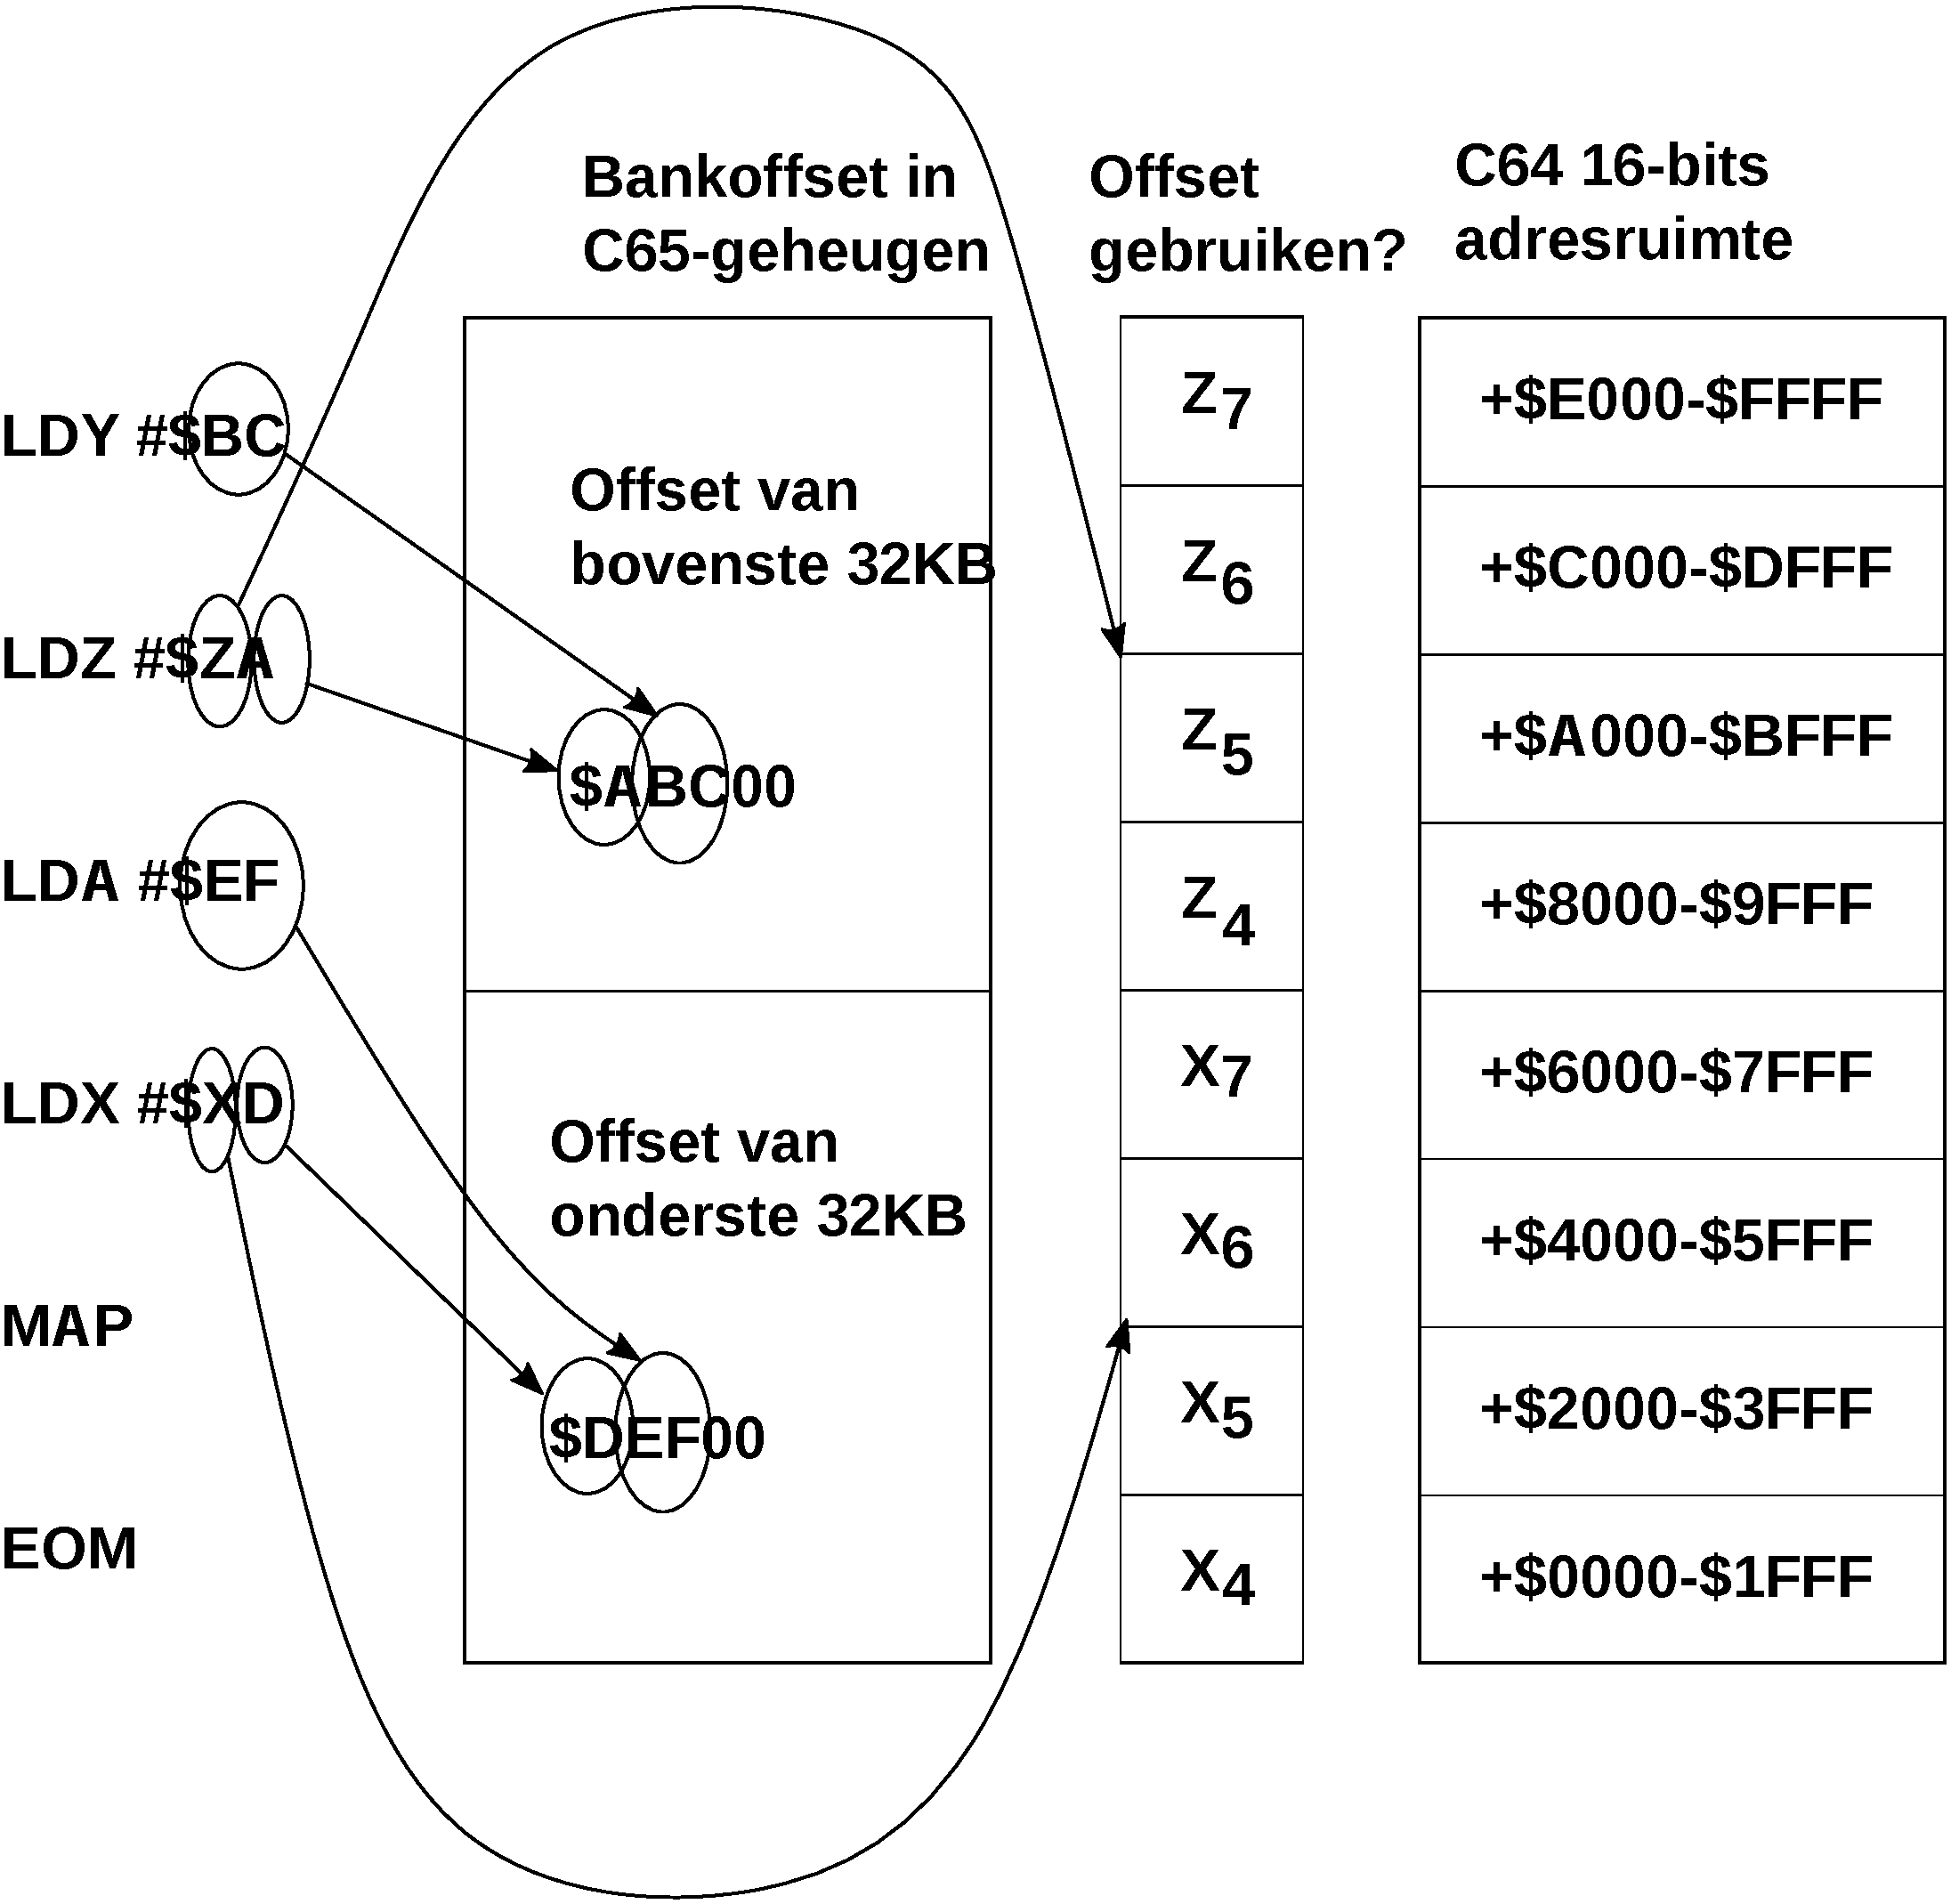
\includegraphics[width=0.75\textwidth]{dutch/images/illustrations/map-instruction-operation.pdf}\index{MAP}\index{Geheugenbanking}
\end{center}

De inhoud van het A-register en de onderste nibble van het X-register vormen samen een 12-bit waarde die met 256 wordt vermenigvuldigd om de offset te produceren die wordt gebruikt voor elk van de 8KB-banken in het onderste 32KB-gedeelte van de 16-bit adresruimte van de 6502. De bovenste nibble van het X-register wordt als vlaggen gebruikt om aan te geven welke van de vier 8KB-blokken in dat 32KB-gedeelte van de 6502-adresruimte de offset bij hun adres moeten optellen om het werkelijke adres te berekenen.

De Y- en Z-registers worden op vergelijkbare manier gebruikt om de offset te produceren voor het bovenste 32KB-gedeelte van de 6502-adresruimte, en de vlaggen om aan te geven of de offset wordt gebruikt voor elk van de vier 8KB-blokken in dat gedeelte van de adresruimte.

De onderste 8 bits van de offset kunnen niet worden ingesteld. De offset is dus een veelvoud van 256 bytes, in tegenstelling tot sommige uitgebreide 6502-processoren. In de praktijk is deze beperking echter zelden van invloed.

Om te begrijpen hoe dit in de praktijk werkt, laat het volgende voorbeeld zien hoe dit werkt met een concreet voorbeeld, met de adresbereiken die zichtbaar zijn in elk van de 8KB-segmenten van de 64KB-adresruimte van de 6502:

\begin{center}
  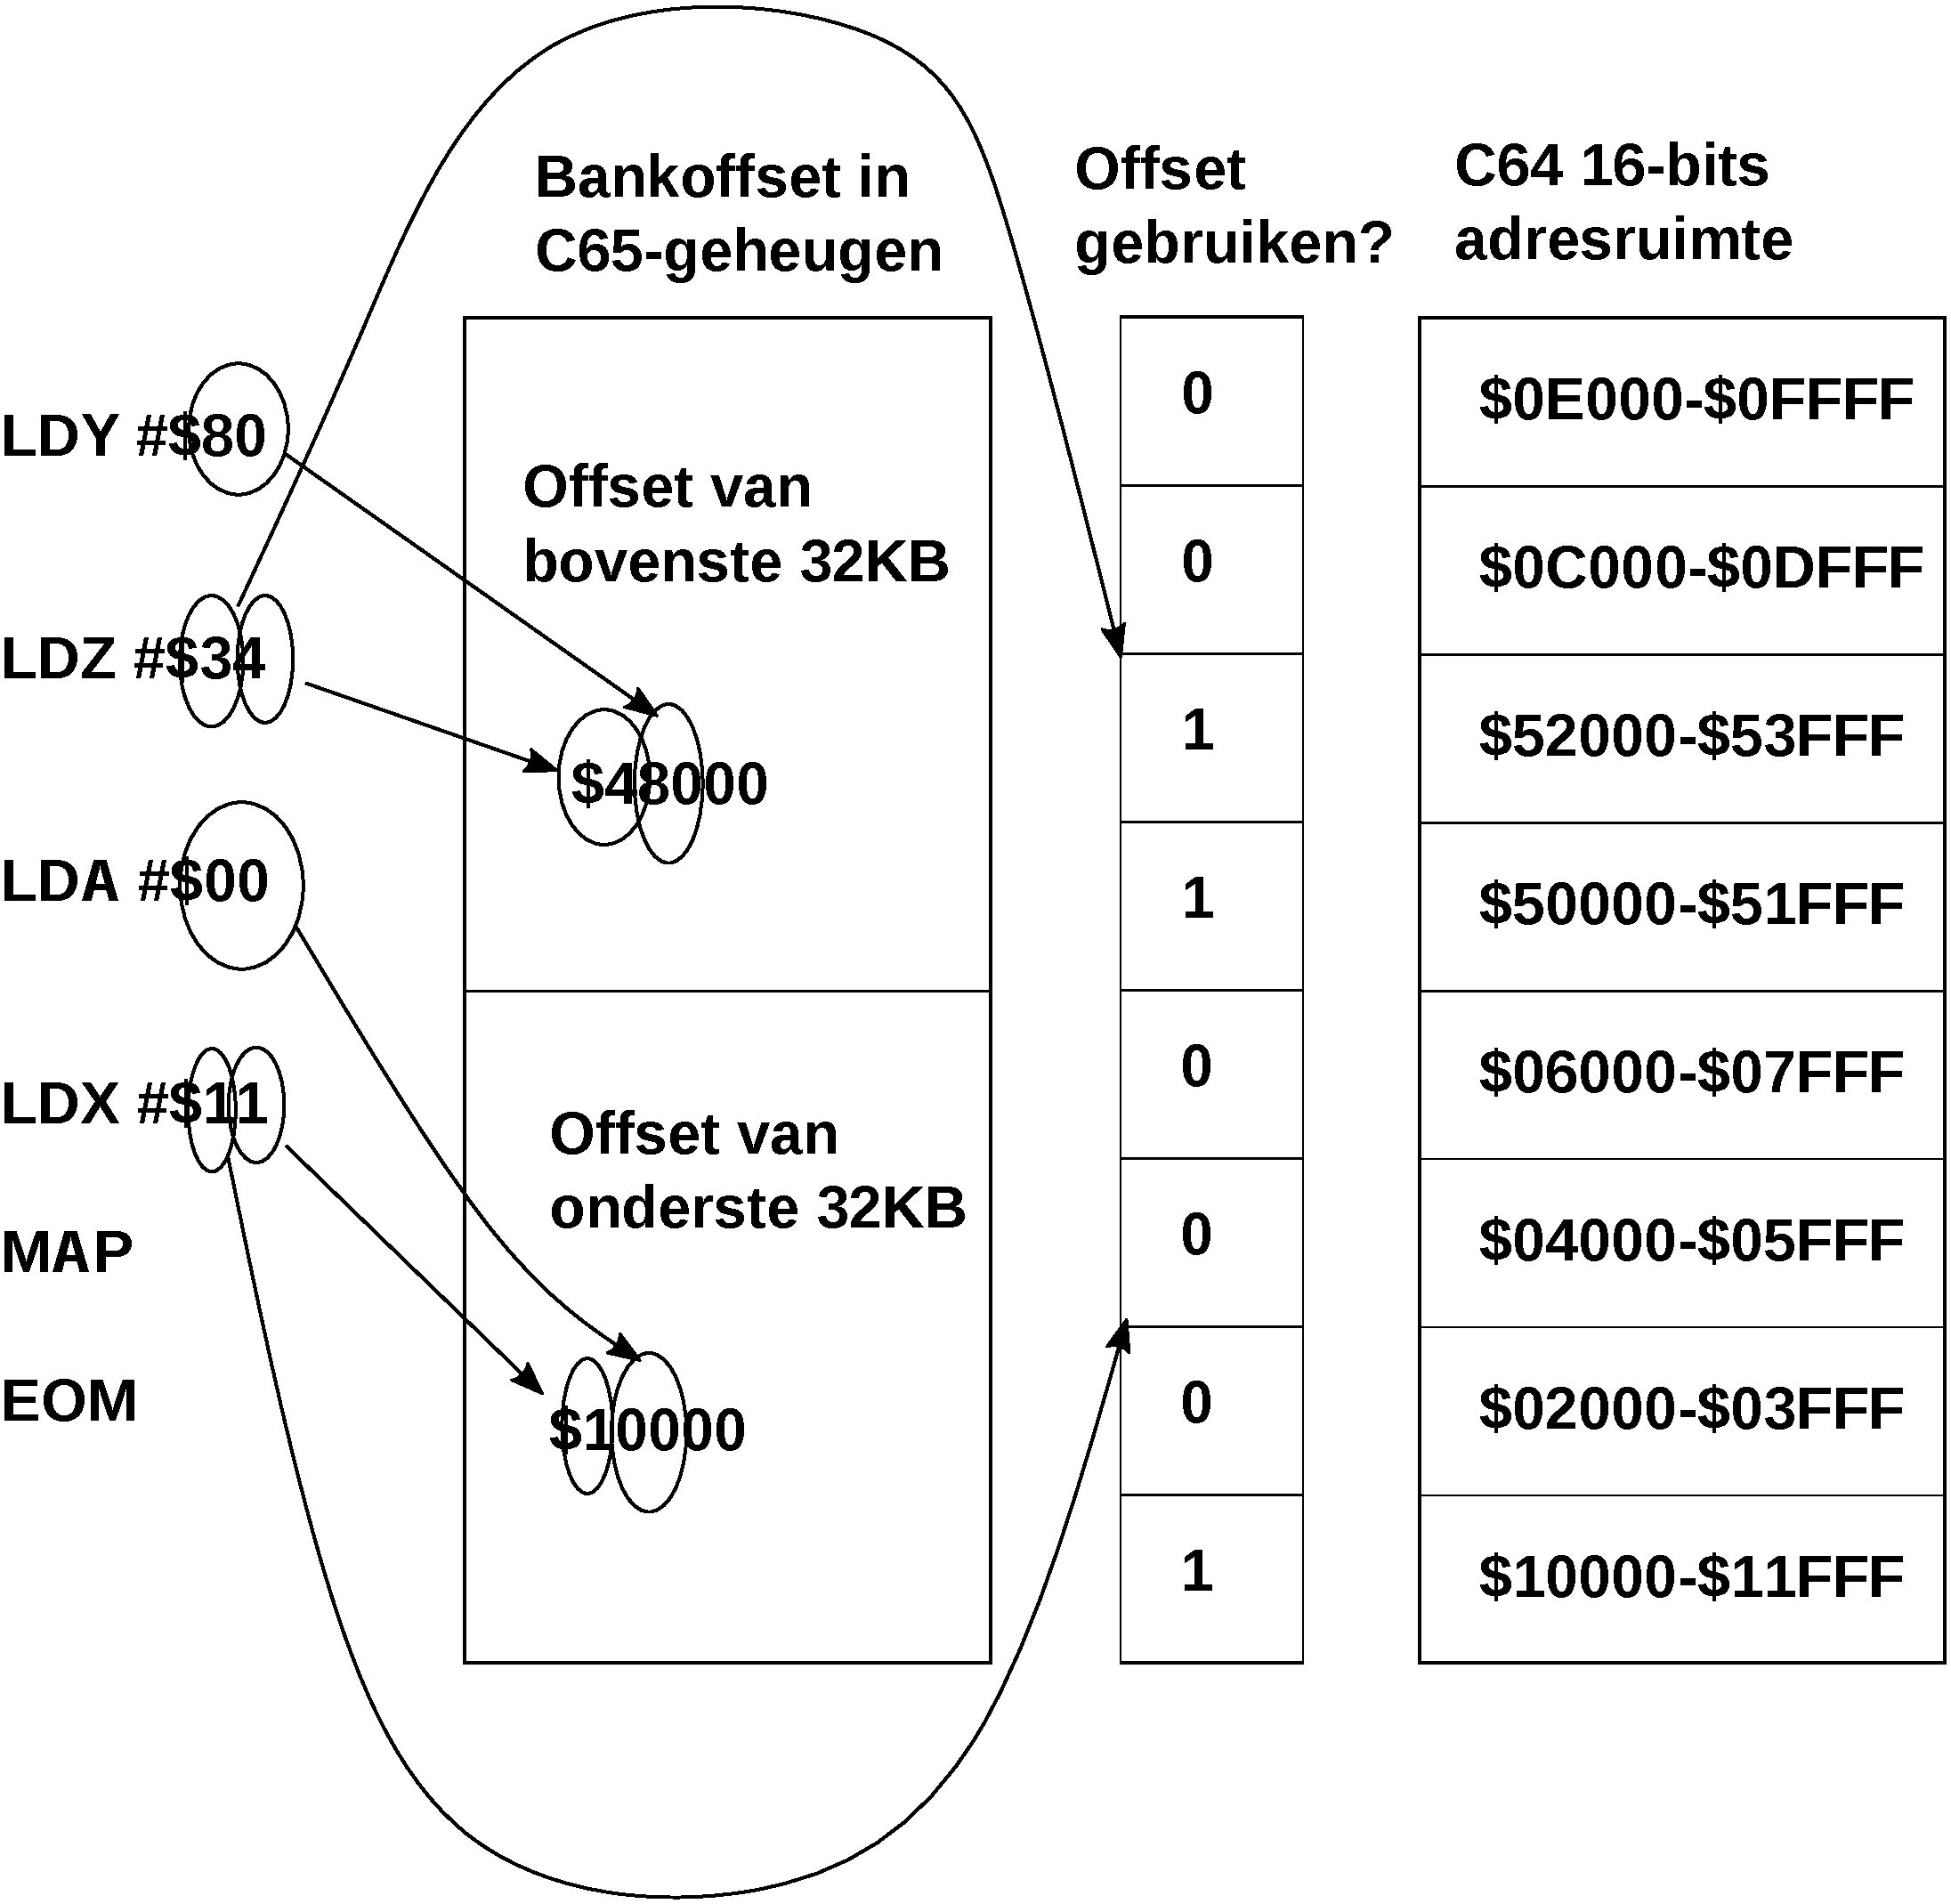
\includegraphics[width=0.75\textwidth]{dutch/images/illustrations/map-instruction-operation-example1.pdf}\index{MAP}\index{Geheugenbanking}
\end{center}

Merk op dat de offsets voor elk van de twee 32KB-adresbereiken worden opgeteld bij het 6502-adres. Vandaar dat de offset van \$48000 voor het bovenste 32KB-gedeelte een adres van \$50000 genereert bij het 6502-adres \$8000.

Zie ook ``De MAP-instructie gebruiken om >1MB te benaderen'' voor verdere uitleg.

\subsubsection{DMA-controller}

De F018/F018A DMA-controller van de C65 maakt het mogelijk om gegevens in het geheugen op willekeurige locaties in de 1MB-adresruimte snel te vullen, te kopiëren en te wisselen. Gedetailleerde informatie over de F018 DMA-controller en de verbeteringen die de MEGA65 daarop heeft aangebracht, vindt u in \bookvref{cha:dmagic}

\subsubsection{Platte geheugentoegang}

\subsection{Toegang tot geheugen buiten het 1MB-punt}
\label{sec:extended-memory}

De MEGA65 kan tot 256MB geheugen ondersteunen. Dit is meer dan de 1MB-adresruimte van de CSG4510 waarop deze is gebaseerd. Er zijn verschillende manieren om dit te bereiken.

\subsubsection{De MAP-instructie gebruiken om >1MB te benaderen}

De volledige adresruimte is beschikbaar voor de MAP-instructie voor traditionele C65-stijl geheugenmapping, hoewel enige voorzichtigheid geboden is, omdat de MAP-instructie tot drie keer moet worden aangeroepen. De reden hiervoor is dat de MAP-instructie eerst moet worden aangeroepen om te selecteren welk megabyte geheugen zal worden gebruikt voor de onderste en bovenste mapregio's, voordat deze opnieuw op de normale manier wordt aangeroepen om de geheugenmapping in te stellen. Omdat tussen deze twee aanroepen de geheugenmapping-offset een mix van oude en nieuwe adressen zal zijn, moet alle mapping eerst worden uitgeschakeld via de MAP-instructie. Dit betekent dat de code voor het hermappen van geheugen zich in het onderste 64KB RAM of in een van de ROM-bankbare regio's moet bevinden, zodat deze tijdens het mappingproces zichtbaar blijft.

Als deze situatie niet goed wordt afgehandeld, zal de processor instructies uitvoeren vanuit een onverwachte geheugenlocatie halverwege het proces, doordat de routine die hij uitvoert om de mapping uit te voeren plotseling niet meer in het geheugen gemapt is.

Vanwege de relatieve complexiteit van dit proces en de andere beperkingen van de MAP-instructie als middel om geheugen te benaderen, raden we u aan om voor gegevens buiten de huidige geheugenindeling ofwel DMA of de flat-memory adresvoorzieningen van de 45GS02 te gebruiken die hieronder worden beschreven. Toegang tot de volledige adresruimte via de MAP-instructie is alleen beschikbaar voor de volledigheid.

Als een ander voorbeeld van hoe de MAP-instructie kan worden gebruikt om een geheugengebied uit de uitgebreide adresruimte te mappen, laat het volgende programma de Ethernet-framebuffer vanaf de natuurlijke locatie op \$FFDE8000 op \$6800 verschijnen. Om het voorbeeld zo eenvoudig mogelijk te houden, gaan we ervan uit dat de code in het onderste 64KB RAM draait en niet in het gebied tussen \$6000 -- \$8000.

Omdat de MAP-instructie normaal gesproken alleen de C65-stijl 20-bit adressen kent, moet de MEGA65-uitbreiding op de instructie worden gebruikt om de bovenste 8 bits van de 28-bit MEGA65-adressen in te stellen, dat wil zeggen welk megabyte adresruimte moet worden gebruikt voor de adresvertaling. Dit wordt gedaan door het X-register in te stellen op \$0F wanneer het megabyte-nummer voor de onderste 32KB van de C64-stijl 64KB-adresruimte wordt gedefinieerd. Dit veroorzaakt geen incompatibiliteit met enig redelijk gebruik van de MAP-instructie op een C65, omdat deze waarde aangeeft dat geen van de vier 8KB-geheugenblokken opnieuw zal worden gemapt, maar tegelijkertijd specificeert dat de bovenste 4 bits van de adresoffset voor het hergemapte blok de niet-nul-waarde \$F vormt. Het megabyte-nummer wordt vervolgens gespecificeerd door het A-register in te stellen.

Dezelfde aanpak geldt voor de bovenste 32KB, maar met de Z- en Y-registers in plaats van de X- en A-registers. In dit geval hoeven we de bovenste 32KB geheugen niet te hermappen; we laten de Z- en Y-registers op nul staan. We moeten echter X en A instellen om het megabyte-nummer voor de onderste 32KB op \$FF te zetten. A moet dus de waarde \$FF hebben. Om de onderste 20 bits van de adresoffset in te stellen, gebruiken we de MAP-instructie een tweede keer, dit keer op de normale C65-manier. Omdat we \$6800 naar \$FFDE800 willen hermappen en al met de \$FFxxxxx-offset via het megabyte-nummer hebben afgerekend, hoeven we alleen de offset toe te passen zodat \$6800 naar \$DE800 wijst. \$DE800 minus \$6800 = \$D8000. Omdat de MAP-instructie werkt met een hermappinggranulariteit van 256 bytes = \$100, kunnen we de laatste twee cijfers van \$D8000 laten vallen om de MAP-offset van \$D80 te verkrijgen. De onderste 8 bits, \$80, moeten in het A-register worden geladen. De bovenste 4 bits, \$D, moeten in de onderste nibble van het X-register worden geladen. Omdat we de mapping alleen op het vierde van de vier 8KB-blokken willen toepassen die de onderste 32KB-helft van de C64-geheugenindeling vormen, moeten we het 4e bit van de bovenste nibble instellen. Dat wil zeggen, de bovenste nibble moet worden ingesteld op \%1000, oftewel \$8. Het X-register moet dus worden geladen met \$8D. Hiermee verkrijgen we het volledige voorbeeldprogramma:

\begin{screencode}
; Map de Ethernet-registers op $6000 - $7FFF

; De Ethernet-controller bevindt zich feitelijk op $FFDE000 - $FFDEFFF, dus selecteer de $FF-megabytesectie voor MAP LO
LDA #$ff
LDX #$0f
LDY #$00
LDZ #$00
map

; Activeer nu het mappen van $DE000-$DFFFF op $6000
; De MAP's zijn op offset gebaseerd, dus moet $6000 van het doeladres worden afgetrokken
; $DE000 - $6000 = $D8000
LDA #$80
LDX #$8d
LDY #$00
LDZ #$00
map
EOM

; De Ethernet-buffer is nu zichtbaar op $6800 - $6FFF
\end{screencode}

De EOM (End Of Mapping)-instructie (hetzelfde als NOP op een 6502, oftewel opcode \$EA) werd alleen na de laatste MAP-instructie opgenomen om er zeker van te zijn dat er geen interrupts konden optreden terwijl de geheugenindeling gemengde waarden bevatte met het megabyte-nummer ingesteld, maar de onderste bits van het mappingadres nog niet waren bijgewerkt.

Er is geen voorbeeld in BASIC voor de MAP-instructie mogelijk, omdat de MAP een machinetaalinstructie is van de 4510/45GS02-processoren.

\subsubsection{Platte geheugentoegang}

De 45GS02 maakt het eenvoudig om een byte vanuit elke geheugenlocatie te lezen of te schrijven door de Zero-Page Indirect-adresseermethode een 32-bit pointer te laten gebruiken in plaats van de gebruikelijke 16-bit pointer. Dit wordt bereikt door de Z-geïndexeerde Zero-Page Indirect-adresseermethode voor de toegang te gebruiken, en de instructie direct te laten voorafgaan door een NOP-instructie (opcode \$EA). Bijvoorbeeld:

\begin{screencode}
NOP
LDA ($45),Z
\end{screencode}

Als u de ACME-assembler of een andere assembler gebruikt die de 45GS02-uitbreidingen ondersteunt, kunt u in plaats daarvan vierkante haakjes gebruiken om aan te geven dat u een flat-memory-bewerking uitvoert. Dergelijke assemblers voegen de \$EA-prefix automatisch voor u in. Bijvoorbeeld:

\begin{screencode}
LDA [$45],Z
\end{screencode}

Ongeacht welk hulpmiddel u gebruikt, in dit voorbeeld zouden de vier bytes Zero-Page-geheugen op \$45 -- \$48 lezen om een 32-bit geheugenadres te vormen, en de waarde van het Z-register hieraan optellen om het werkelijke adres te vormen waaruit wordt gelezen. De bytevolgorde in het adres is hetzelfde als bij de 6502, oftewel het rechtse (minst significante) byte van het adres wordt als eerste gelezen vanaf het eerste adres (\$45 in dit geval), enzovoort, totdat het meest linkse (meest significante) byte wordt gelezen vanaf \$48. Om bijvoorbeeld vanaf geheugenlocatie \$12345678 te lezen, moet de inhoud van het geheugen beginnend op \$45 bestaan uit 78 56 34 12.

Deze methode is veel efficiënter en ook eenvoudiger dan het gebruik van de MAP-instructie of de DMA-controller voor enkelvoudige geheugentoegangen, en is wat wij doorgaans aanbevelen. De DMA-controller kan worden gebruikt voor het verplaatsen/vullen van grotere geheugenregio's. Wij bevelen de MAP-instructie alleen aan voor het banken van code, of in zeldzame situaties waarbij uitgebreide toegang tot een klein geheugengebied vereist is en de extra cycli voor het lezen van de 32-bit-adressen problematisch zijn.

\subsection{Virtueel 32-bit-register}

De 45GS02 maakt het mogelijk om zijn vier algemene registers, A, X, Y en Z (A is LSB, Z is MSB), als één enkel virtueel 32-bit-register te gebruiken, ook wel het {\em Q-pseudoregister} genoemd. Dit kan veelvoorkomende bewerkingen aanzienlijk vereenvoudigen en versnellen, en helpt veelvoorkomende programmeerfouten te voorkomen. Het optellen van twee 16-bit- of 32-bit-waarden kan bijvoorbeeld eenvoudig worden uitgevoerd met iets als:

\begin{screencode}
  ; Wis de carry vóór het optellen, zoals gebruikelijk
  CLC
  ; Laat twee NEG-instructies voorafgaan om de virtuele 32-bit-registermodus te selecteren
  NEG
  NEG
  LDA $1234  ; Laadt de inhoud van $1234-$1237 in respectievelijk A, X, Y en Z
  ; En nogmaals, voor de optelling
  NEG
  NEG
  ADC $1238  ; Telt de inhoud van $1238-$123B op
  ; Het resultaat van de optelling staat nu in A, X, Y en Z.
  ; En kan geheel of gedeeltelijk worden weggeschreven

  ; Om het geheel weg te schrijven is wederom de NEG + NEG-prefix nodig
  NEG
  NEG
  STA $123C ; Schrijft het geheel weg naar $123C-$123F

  ; Of om de laagste bytes weg te schrijven, kan eenvoudigweg de inhoud van A en X normaal worden weggeschreven
  STA $1240
  STX $1241
\end{screencode}

Deze aanpak werkt met de LDA-, STA-, ADC-, SBC-, CMP-, EOR-, AND-, BIT-, ORA-, ASL-, ASR-, LSR-, ROL-, ROR-, INC- en DEC-instructies. Indien u ACME of een andere 45GS02-ondersteunende assembler gebruikt, kunt u in plaats daarvan de nieuwe \stw{LDQ}, \stw{STQ}, \stw{ADCQ}, \stw{SBCQ}, \stw{CPQ}, \stw{EORQ}, \stw{ANDQ}, \stw{BITQ}, \stw{ORQ}, \stw{ASLQ}, \stw{ASRQ}, \stw{LSRQ}, \stw{ROLQ}, \stw{RORQ}, \stw{INQ} en \stw{DEQ} mnemonics gebruiken.\index{LDQ}\index{STQ}\index{ADCQ}\index{SBCQ}\index{CPQ}\index{EORQ}\index{ANDQ}\index{BITQ}\index{ORQ}\index{ASLQ}\index{ASRQ}\index{LSRQ}\index{ROLQ}\index{RORQ}\index{INQ}\index{DEQ} Het vorige voorbeeld wordt dan:

\begin{screencode}
  ; Wis de carry vóór het optellen, zoals gebruikelijk
  CLC
  LDQ  $1234  ; Laadt de inhoud van $1234-$1237 in respectievelijk A, X, Y en Z
  ADCQ $1238  ; Telt de inhoud van $1238-$123B op
  ; Het resultaat van de optelling staat nu in A, X, Y en Z.
  ; En kan geheel of gedeeltelijk worden weggeschreven

  STQ $123C ; Schrijft het geheel weg naar $123C-$123F

  ; Of om de laagste bytes weg te schrijven, kan eenvoudigweg de inhoud van A en X normaal worden weggeschreven
  STA $1240
  STX $1241
\end{screencode}

De virtuele 32-bit-adresseermethode werkt met elke adresseermethode. Geïndexeerde adresseermethoden, waarbij X, Y of Z bij het adres wordt opgeteld, moeten echter met voorzichtigheid worden gebruikt, omdat deze registers in feite een deel van een 32-bit-waarde kunnen bevatten.

De uitzondering is de Zero-Page Indirect Z-geïndexeerde adresseermethode: in dit geval wordt het Z-register NIET bij het doeladres opgeteld (met uitzondering van de LDQ-opcode), in tegenstelling tot wat normaal het geval is. Hierdoor kan het virtuele 32-bit-register worden gebruikt met platte-geheugentoegang met de gecombineerde prefix \stw{NEG NEG NOP} vóór de instructie, zodat een 32-bit-waarde ergens in het geheugen met één instructie kan worden benaderd.

Merk op dat het virtuele 32-bit-register niet kan worden gebruikt in de immediate-modus, bijvoorbeeld om een constante in de vier algemene registers te laden of om een constante waarde op te tellen of af te trekken. Dit dient om problemen met instructies van variabele lengte te voorkomen.

Voor LDQ en STQ bespaart dit hoogstens één byte ten opzichte van LDA \#\$nn ... LDZ \#\$nn, en zou het niet sneller zijn. Voor veel veelvoorkomende waarden, zoals \#\$00000000, bestaan er zelfs verkortingen, zoals:

\begin{screencode}
LDA #$00
TAX
TAY
TAZ
\end{screencode}

Indien u een 32-bit-immediate-waarde moet optellen of aftrekken, kan dit vereisen dat u de argumenten herschikt of andere kleine aanpassingen uitvoert. Om bijvoorbeeld de som van de inhoud van het geheugen en een immediate-waarde te berekenen, kunt u de A-, X-, Y- en Z-registers laden met de immediate-waarde en vervolgens \stw{ADCQ} gebruiken met het geheugenadres:

\begin{screencode}
  ; Haal de immediate-waarde #$12345678 in Q
  LDA #$78
  LDX #$56
  LDY #$34
  LDZ #$12
  ; Telt de inhoud van de geheugenlocaties $1234-$1237 op
  NEG
  NEG
  ADC $1234
  ; Slaat het resultaat op in $1234-$1237
  NEG
  NEG
  STA $1234
\end{screencode}

Wanneer u opnieuw de ACME- of een andere 45GS02-ondersteunende assembler gebruikt, kan dit compacter en duidelijker worden geschreven als volgt. Merk op dat in beide gevallen dezelfde bytevolgorde van machinetaal wordt geproduceerd en het programma hetzelfde aantal cycli zal kosten om uit te voeren.

\begin{screencode}
  ; Haal de immediate-waarde #$12345678 in Q
  LDA #$78
  LDX #$56
  LDY #$34
  LDZ #$12
  ; Telt de inhoud van de geheugenlocaties $1234-$1237 op
  ADCQ $1234
  ; Slaat het resultaat op in $1234-$1237
  STQ $1234
\end{screencode}

\section{In het geheugen gemapte registers van de C64-CPU}

\setlength{\tabcolsep}{0pt}
\begin{longtable}{|C{12.5mm}|C{12.5mm}|C{12.5mm}|C{12.5mm}|C{12.5mm}|C{12.5mm}|C{12.5mm}|C{12.5mm}|C{12.5mm}|C{12.5mm}|}
\hline
{\bf{HEX}} & {\bf{DEC}} & {\bf{DB7}} & {\bf{DB6}} & {\bf{DB5}} & {\bf{DB4}} & {\bf{DB3}} & {\bf{DB2}} & {\bf{DB1}} & {\bf{DB0}} \\
\hline
\endfirsthead
\multicolumn{3}{l@{}}{\ldots Vervolgd}\\
\hline
{\bf{HEX}} & {\bf{DEC}} & {\bf{DB7}} & {\bf{DB6}} & {\bf{DB5}} & {\bf{DB4}} & {\bf{DB3}} & {\bf{DB2}} & {\bf{DB1}} & {\bf{DB0}} \\
\endhead
\multicolumn{3}{l@{}}{Vervolgd \ldots}\\
\endfoot
\hline
\endlastfoot
\footnotesize  00\index{\$00 (PORTDDR)}\index{PORTDDR} & \footnotesize 0 & \multicolumn{8}{c|}{\footnotesize PORTDDR\index{Registers!PORTDDR}}\\
\hline
\footnotesize  01\index{\$01 (C64MAP)}\index{C64MAP} & \footnotesize 1 & \multicolumn{5}{c|}{\footnotesize PORT\index{Registers!PORT}}& \multicolumn{3}{c|}{\footnotesize C64MAP\index{Registers!C64MAP}}\\
\hline
\end{longtable}
\begin{itemize}
\item{\bf{C64MAP}\index{Registers!C64MAP}} Geheugenmapper van de processorport
\item{\bf{PORT}\index{Registers!PORT}} 6510/45GS10 CPU-portgegevens
\item{\bf{PORTDDR}\index{Registers!PORTDDR}} 6510/45GS10 CPU-port-DDR. Schrijf 65 om de 40MHz-modus af te dwingen, of 64 om de normale snelheidscontroles weer in te schakelen.
\end{itemize}


\section{Nieuwe in het geheugen gemapte CPU-registers}

\setlength{\tabcolsep}{0pt}
\begin{longtable}{|C{12.5mm}|C{12.5mm}|C{12.5mm}|C{12.5mm}|C{12.5mm}|C{12.5mm}|C{12.5mm}|C{12.5mm}|C{12.5mm}|C{12.5mm}|}
\hline
{\bf{HEX}} & {\bf{DEC}} & {\bf{DB7}} & {\bf{DB6}} & {\bf{DB5}} & {\bf{DB4}} & {\bf{DB3}} & {\bf{DB2}} & {\bf{DB1}} & {\bf{DB0}} \\
\hline
\endfirsthead
\multicolumn{3}{l@{}}{\ldots Vervolgd}\\
\hline
{\bf{HEX}} & {\bf{DEC}} & {\bf{DB7}} & {\bf{DB6}} & {\bf{DB5}} & {\bf{DB4}} & {\bf{DB3}} & {\bf{DB2}} & {\bf{DB1}} & {\bf{DB0}} \\
\endhead
\multicolumn{3}{l@{}}{Vervolgd \ldots}\\
\endfoot
\hline
\endlastfoot
\footnotesize  D640\index{Registers!\$D640} \index{Registers!54848} & \footnotesize 54848 & \multicolumn{8}{c|}{\footnotesize HTRAP00\index{Registers!HTRAPXX}}\\
\hline
\footnotesize  D641\index{Registers!\$D641} \index{Registers!54849} & \footnotesize 54849 & \multicolumn{8}{c|}{\footnotesize HTRAP01\index{Registers!HTRAP01}}\\
\hline
\footnotesize  D642\index{Registers!\$D642} \index{Registers!54850} & \footnotesize 54850 & \multicolumn{8}{c|}{\footnotesize HTRAP02\index{Registers!HTRAP02}}\\
\hline
\footnotesize  D643\index{Registers!\$D643} \index{Registers!54851} & \footnotesize 54851 & \multicolumn{8}{c|}{\footnotesize HTRAP03\index{Registers!HTRAP03}}\\
\hline
\footnotesize  D644\index{Registers!\$D644} \index{Registers!54852} & \footnotesize 54852 & \multicolumn{8}{c|}{\footnotesize HTRAP04\index{Registers!HTRAP04}}\\
\hline
\footnotesize  D645\index{Registers!\$D645} \index{Registers!54853} & \footnotesize 54853 & \multicolumn{8}{c|}{\footnotesize HTRAP05\index{Registers!HTRAP05}}\\
\hline
\footnotesize  D646\index{Registers!\$D646} \index{Registers!54854} & \footnotesize 54854 & \multicolumn{8}{c|}{\footnotesize HTRAP06\index{Registers!HTRAP06}}\\
\hline
\footnotesize  D647\index{Registers!\$D647} \index{Registers!54855} & \footnotesize 54855 & \multicolumn{8}{c|}{\footnotesize HTRAP07\index{Registers!HTRAP07}}\\
\hline
\footnotesize  D648\index{Registers!\$D648} \index{Registers!54856} & \footnotesize 54856 & \multicolumn{8}{c|}{\footnotesize HTRAP08\index{Registers!HTRAP08}}\\
\hline
\footnotesize  D649\index{Registers!\$D649} \index{Registers!54857} & \footnotesize 54857 & \multicolumn{8}{c|}{\footnotesize HTRAP09\index{Registers!HTRAP09}}\\
\hline
\footnotesize  D64A\index{Registers!\$D64A} \index{Registers!54858} & \footnotesize 54858 & \multicolumn{8}{c|}{\footnotesize HTRAP0A\index{Registers!HTRAP0A}}\\
\hline
\footnotesize  D64B\index{Registers!\$D64B} \index{Registers!54859} & \footnotesize 54859 & \multicolumn{8}{c|}{\footnotesize HTRAP0B\index{Registers!HTRAP0B}}\\
\hline
\footnotesize  D64C\index{Registers!\$D64C} \index{Registers!54860} & \footnotesize 54860 & \multicolumn{8}{c|}{\footnotesize HTRAP0C\index{Registers!HTRAP0C}}\\
\hline
\footnotesize  D64D\index{Registers!\$D64D} \index{Registers!54861} & \footnotesize 54861 & \multicolumn{8}{c|}{\footnotesize HTRAP0D\index{Registers!HTRAP0D}}\\
\hline
\footnotesize  D64E\index{Registers!\$D64E} \index{Registers!54862} & \footnotesize 54862 & \multicolumn{8}{c|}{\footnotesize HTRAP0E\index{Registers!HTRAP0E}}\\
\hline
\footnotesize  D64F\index{Registers!\$D64F} \index{Registers!54863} & \footnotesize 54863 & \multicolumn{8}{c|}{\footnotesize HTRAP0F\index{Registers!HTRAP0F}}\\
\hline
\footnotesize  D650\index{Registers!\$D650} \index{Registers!54864} & \footnotesize 54864 & \multicolumn{8}{c|}{\footnotesize HTRAP10\index{Registers!HTRAP10}}\\
\hline
\footnotesize  D651\index{Registers!\$D651} \index{Registers!54865} & \footnotesize 54865 & \multicolumn{8}{c|}{\footnotesize HTRAP11\index{Registers!HTRAP11}}\\
\hline
\footnotesize  D652\index{Registers!\$D652} \index{Registers!54866} & \footnotesize 54866 & \multicolumn{8}{c|}{\footnotesize HTRAP12\index{Registers!HTRAP12}}\\
\hline
\footnotesize  D653\index{Registers!\$D653} \index{Registers!54867} & \footnotesize 54867 & \multicolumn{8}{c|}{\footnotesize HTRAP13\index{Registers!HTRAP13}}\\
\hline
\footnotesize  D654\index{Registers!\$D654} \index{Registers!54868} & \footnotesize 54868 & \multicolumn{8}{c|}{\footnotesize HTRAP14\index{Registers!HTRAP14}}\\
\hline
\footnotesize  D655\index{Registers!\$D655} \index{Registers!54869} & \footnotesize 54869 & \multicolumn{8}{c|}{\footnotesize HTRAP15\index{Registers!HTRAP15}}\\
\hline
\footnotesize  D656\index{Registers!\$D656} \index{Registers!54870} & \footnotesize 54870 & \multicolumn{8}{c|}{\footnotesize HTRAP16\index{Registers!HTRAP16}}\\
\hline
\footnotesize  D657\index{Registers!\$D657} \index{Registers!54871} & \footnotesize 54871 & \multicolumn{8}{c|}{\footnotesize HTRAP17\index{Registers!HTRAP17}}\\
\hline
\footnotesize  D658\index{Registers!\$D658} \index{Registers!54872} & \footnotesize 54872 & \multicolumn{8}{c|}{\footnotesize HTRAP18\index{Registers!HTRAP18}}\\
\hline
\footnotesize  D659\index{Registers!\$D659} \index{Registers!54873} & \footnotesize 54873 & \multicolumn{8}{c|}{\footnotesize HTRAP19\index{Registers!HTRAP19}}\\
\hline
\footnotesize  D65A\index{Registers!\$D65A} \index{Registers!54874} & \footnotesize 54874 & \multicolumn{8}{c|}{\footnotesize HTRAP1A\index{Registers!HTRAP1A}}\\
\hline
\footnotesize  D65B\index{Registers!\$D65B} \index{Registers!54875} & \footnotesize 54875 & \multicolumn{8}{c|}{\footnotesize HTRAP1B\index{Registers!HTRAP1B}}\\
\hline
\footnotesize  D65C\index{Registers!\$D65C} \index{Registers!54876} & \footnotesize 54876 & \multicolumn{8}{c|}{\footnotesize HTRAP1C\index{Registers!HTRAP1C}}\\
\hline
\footnotesize  D65D\index{Registers!\$D65D} \index{Registers!54877} & \footnotesize 54877 & \multicolumn{8}{c|}{\footnotesize HTRAP1D\index{Registers!HTRAP1D}}\\
\hline
\footnotesize  D65E\index{Registers!\$D65E} \index{Registers!54878} & \footnotesize 54878 & \multicolumn{8}{c|}{\footnotesize HTRAP1E\index{Registers!HTRAP1E}}\\
\hline
\footnotesize  D65F\index{Registers!\$D65F} \index{Registers!54879} & \footnotesize 54879 & \multicolumn{8}{c|}{\footnotesize HTRAP1F\index{Registers!HTRAP1F}}\\
\hline
\footnotesize  D660\index{Registers!\$D660} \index{Registers!54880} & \footnotesize 54880 & \multicolumn{8}{c|}{\footnotesize HTRAP20\index{Registers!HTRAP20}}\\
\hline
\footnotesize  D661\index{Registers!\$D661} \index{Registers!54881} & \footnotesize 54881 & \multicolumn{8}{c|}{\footnotesize HTRAP21\index{Registers!HTRAP21}}\\
\hline
\footnotesize  D662\index{Registers!\$D662} \index{Registers!54882} & \footnotesize 54882 & \multicolumn{8}{c|}{\footnotesize HTRAP22\index{Registers!HTRAP22}}\\
\hline
\footnotesize  D663\index{Registers!\$D663} \index{Registers!54883} & \footnotesize 54883 & \multicolumn{8}{c|}{\footnotesize HTRAP23\index{Registers!HTRAP23}}\\
\hline
\footnotesize  D664\index{Registers!\$D664} \index{Registers!54884} & \footnotesize 54884 & \multicolumn{8}{c|}{\footnotesize HTRAP24\index{Registers!HTRAP24}}\\
\hline
\footnotesize  D665\index{Registers!\$D665} \index{Registers!54885} & \footnotesize 54885 & \multicolumn{8}{c|}{\footnotesize HTRAP25\index{Registers!HTRAP25}}\\
\hline
\footnotesize  D666\index{Registers!\$D666} \index{Registers!54886} & \footnotesize 54886 & \multicolumn{8}{c|}{\footnotesize HTRAP26\index{Registers!HTRAP26}}\\
\hline
\footnotesize  D667\index{Registers!\$D667} \index{Registers!54887} & \footnotesize 54887 & \multicolumn{8}{c|}{\footnotesize HTRAP27\index{Registers!HTRAP27}}\\
\hline
\footnotesize  D668\index{Registers!\$D668} \index{Registers!54888} & \footnotesize 54888 & \multicolumn{8}{c|}{\footnotesize HTRAP28\index{Registers!HTRAP28}}\\
\hline
\footnotesize  D669\index{Registers!\$D669} \index{Registers!54889} & \footnotesize 54889 & \multicolumn{8}{c|}{\footnotesize HTRAP29\index{Registers!HTRAP29}}\\
\hline
\footnotesize  D66A\index{Registers!\$D66A} \index{Registers!54890} & \footnotesize 54890 & \multicolumn{8}{c|}{\footnotesize HTRAP2A\index{Registers!HTRAP2A}}\\
\hline
\footnotesize  D66B\index{Registers!\$D66B} \index{Registers!54891} & \footnotesize 54891 & \multicolumn{8}{c|}{\footnotesize HTRAP2B\index{Registers!HTRAP2B}}\\
\hline
\footnotesize  D66C\index{Registers!\$D66C} \index{Registers!54892} & \footnotesize 54892 & \multicolumn{8}{c|}{\footnotesize HTRAP2C\index{Registers!HTRAP2C}}\\
\hline
\footnotesize  D66D\index{Registers!\$D66D} \index{Registers!54893} & \footnotesize 54893 & \multicolumn{8}{c|}{\footnotesize HTRAP2D\index{Registers!HTRAP2D}}\\
\hline
\footnotesize  D66E\index{Registers!\$D66E} \index{Registers!54894} & \footnotesize 54894 & \multicolumn{8}{c|}{\footnotesize HTRAP2E\index{Registers!HTRAP2E}}\\
\hline
\footnotesize  D66F\index{Registers!\$D66F} \index{Registers!54895} & \footnotesize 54895 & \multicolumn{8}{c|}{\footnotesize HTRAP2F\index{Registers!HTRAP2F}}\\
\hline
\footnotesize  D670\index{Registers!\$D670} \index{Registers!54896} & \footnotesize 54896 & \multicolumn{8}{c|}{\footnotesize HTRAP30\index{Registers!HTRAP30}}\\
\hline
\footnotesize  D671\index{Registers!\$D671} \index{Registers!54897} & \footnotesize 54897 & \multicolumn{8}{c|}{\footnotesize HTRAP31\index{Registers!HTRAP31}}\\
\hline
\footnotesize  D672\index{Registers!\$D672} \index{Registers!54898} & \footnotesize 54898 & \multicolumn{8}{c|}{\footnotesize HTRAP32\index{Registers!HTRAP32}}\\
\hline
\footnotesize  D673\index{Registers!\$D673} \index{Registers!54899} & \footnotesize 54899 & \multicolumn{8}{c|}{\footnotesize HTRAP33\index{Registers!HTRAP33}}\\
\hline
\footnotesize  D674\index{Registers!\$D674} \index{Registers!54900} & \footnotesize 54900 & \multicolumn{8}{c|}{\footnotesize HTRAP34\index{Registers!HTRAP34}}\\
\hline
\footnotesize  D675\index{Registers!\$D675} \index{Registers!54901} & \footnotesize 54901 & \multicolumn{8}{c|}{\footnotesize HTRAP35\index{Registers!HTRAP35}}\\
\hline
\footnotesize  D676\index{Registers!\$D676} \index{Registers!54902} & \footnotesize 54902 & \multicolumn{8}{c|}{\footnotesize HTRAP36\index{Registers!HTRAP36}}\\
\hline
\footnotesize  D677\index{Registers!\$D677} \index{Registers!54903} & \footnotesize 54903 & \multicolumn{8}{c|}{\footnotesize HTRAP37\index{Registers!HTRAP37}}\\
\hline
\footnotesize  D678\index{Registers!\$D678} \index{Registers!54904} & \footnotesize 54904 & \multicolumn{8}{c|}{\footnotesize HTRAP38\index{Registers!HTRAP38}}\\
\hline
\footnotesize  D679\index{Registers!\$D679} \index{Registers!54905} & \footnotesize 54905 & \multicolumn{8}{c|}{\footnotesize HTRAP39\index{Registers!HTRAP39}}\\
\hline
\footnotesize  D67A\index{Registers!\$D67A} \index{Registers!54906} & \footnotesize 54906 & \multicolumn{8}{c|}{\footnotesize HTRAP3A\index{Registers!HTRAP3A}}\\
\hline
\footnotesize  D67B\index{Registers!\$D67B} \index{Registers!54907} & \footnotesize 54907 & \multicolumn{8}{c|}{\footnotesize HTRAP3B\index{Registers!HTRAP3B}}\\
\hline
\footnotesize  D67C\index{Registers!\$D67C} \index{Registers!54908} & \footnotesize 54908 & \multicolumn{8}{c|}{\footnotesize HTRAP3C\index{Registers!HTRAP3C}}\\
\hline
\footnotesize  D67D\index{Registers!\$D67D} \index{Registers!54909} & \footnotesize 54909 & \multicolumn{8}{c|}{\footnotesize HTRAP3D\index{Registers!HTRAP3D}}\\
\hline
\footnotesize  D67E\index{Registers!\$D67E} \index{Registers!54910} & \footnotesize 54910 & \multicolumn{8}{c|}{\footnotesize HTRAP3E\index{Registers!HTRAP3E}}\\
\hline
\footnotesize  D67F\index{Registers!\$D67F} \index{Registers!54911} & \footnotesize 54911 & \multicolumn{8}{c|}{\footnotesize HTRAP3F\index{Registers!HTRAP3F}}\\
\hline
\footnotesize  D710\index{Registers!\$D710} \index{Registers!55056} & \footnotesize 55056 & \multicolumn{2}{c|}{\footnotesize --}& \multicolumn{2}{c|}{\footnotesize BADEXTRA\index{Registers!BADEXTRA}}& \footnotesize BRCOST & \footnotesize -- & \footnotesize SLIEN & \footnotesize BADLEN \\
\hline
\footnotesize  D7EF\index{Registers!\$D7EF} \index{Registers!55279} & \footnotesize 55279 & \multicolumn{8}{c|}{\footnotesize HWRNG\-RAND\index{Registers!HWRNGRAND}}\\
\hline
\footnotesize  D7FA\index{Registers!\$D7FA} \index{Registers!55290} & \footnotesize 55290 & \multicolumn{8}{c|}{\footnotesize FRAMECOUNT\index{Registers!FRAMECOUNT}}\\
\hline
\footnotesize  D7FB\index{Registers!\$D7FB} \index{Registers!55291} & \footnotesize 55291 & \multicolumn{6}{c|}{\footnotesize --}& \footnotesize CARTEN & \footnotesize -- \\
\hline
\footnotesize  D7FD\index{Registers!\$D7FD} \index{Registers!55293} & \footnotesize 55293 & \footnotesize NOEXROM & \footnotesize NOGAME & \multicolumn{5}{c|}{\footnotesize --}& \footnotesize POWEREN \\
\hline
\footnotesize  D7FE\index{Registers!\$D7FE} \index{Registers!55294} & \footnotesize 55294 & \footnotesize HWRNG\-NOTRDY & \footnotesize -- & \footnotesize SLOWSDRAM & \footnotesize SELSDRAM & \footnotesize SLOWCACHE\-ADV & \footnotesize SLOWCACHE & \footnotesize OCEANA & \footnotesize PREFETCH \\
\hline
\end{longtable}
\begin{itemize}
\item{\bf{BADEXTRA}\index{Registers!BADEXTRA}} Kosten van badlines minus 40. D.w.z. 00=40 cycli, 11 = 43 cycli.
\item{\bf{BADLEN}\index{Registers!BADLEN}} Schakelt badline-emulatie in
\item{\bf{BRCOST}\index{Registers!BRCOST}} 1=extra cyclus(sen) rekenen voor genomen vertakkingen
\item{\bf{CARTEN}\index{Registers!CARTEN}} 1=cartridges inschakelen
\item{\bf{FRAMECOUNT}\index{Registers!FRAMECOUNT}} Telt het aantal verstreken videoframes
\item{\bf{HTRAPXX}\index{Registers!HTRAPXX}} Schrijven activeert een hypervisor-trap \$XX
\item{\bf{HWRNGNOTRDY}\index{Registers!HWRNGNOTRDY}} Echte RNG-willekeurig getal van de hardware nog niet gereed (alleen-lezen)
\item{\bf{HWRNGRAND}\index{Registers!HWRNGRAND}} Echt willekeurig getal van de hardware-RNG (lezen activeert de generatie)
\item{\bf{NOEXROM}\index{Registers!NOEXROM}} Overschrijving voor /EXROM: moet 0 zijn om het /EXROM-signaal in te schakelen
\item{\bf{NOGAME}\index{Registers!NOGAME}} Overschrijving voor /GAME: moet 0 zijn om het /GAME-signaal in te schakelen
\item{\bf{OCEANA}\index{Registers!OCEANA}} Schakelt emulatie van cartridge van het type Ocean A in
\item{\bf{POWEREN}\index{Registers!POWEREN}} Zet op nul om de computer uit te schakelen op ondersteunde systemen. ALLEEN-SCHRIJVEN.
\item{\bf{PREFETCH}\index{Registers!PREFETCH}} Schakelt de prefetchlogica voor uitgebreid RAM in
\item{\bf{SELSDRAM}\index{Registers!SELSDRAM}} Selecteert SDRAM in plaats van HyperRAM voor Attic RAM waar beschikbaar
\item{\bf{SLIEN}\index{Registers!SLIEN}} Schakelt interrupts in stijl 6502 (langzaam, 7 cycli) in
\item{\bf{SLOWCACHE}\index{Registers!SLOWCACHE}} Schakelt langzamere regelcaching voor Attic RAM in
\item{\bf{SLOWCACHEADV}\index{Registers!SLOWCACHEADV}} Schakelt de geavanceerde langzamere regelcaching voor Attic RAM in
\item{\bf{SLOWSDRAM}\index{Registers!SLOWSDRAM}} Selecteert de langzame (81MHz) SDRAM-klok
\end{itemize}


\section{MEGA65 CPU-versnellingsregisters voor wiskunde}

Elke MEGA65 bevat een gecombineerde 32-bit-hardwarevermenigvuldiger en -deler. Dit apparaat neemt twee 32-bit-invoeren, {\bf MULTINA} en {\bf MULTINB}, en berekent tegelijkertijd:

\begin{itemize}
\item het 64-bit-product {\bf MULTOUT} van {\bf MULTINA} en {\bf MULTINB}\item het 32-bit-gehele deel {\bf DIVOUT}(4-7) van {\bf MULTINA} gedeeld door {\bf MULTINB}\item het 32-bit-breukdeel {\bf DIVOUT}(0-3) van {\bf MULTINA} gedeeld door {\bf MULTINB}
\end{itemize}

De uitvoer wordt altijd op basis van de invoer bijgewerkt, zodat er geen speciale actie nodig is bij het wijzigen van de invoer. De vermenigvuldiger heeft 1 cyclus nodig om te berekenen, zodat het bijgewerkte resultaat onmiddellijk beschikbaar is (een {\bf MULBUSY}-bit is gedefinieerd, maar deze zal momenteel niet worden gezet). De hardwaredeler kan echter tot 20 cycli kosten, afhankelijk van de specifieke invoer. De programmeur moet de {\bf DIVBUSY}-bit controleren indien de deler nog bezig is met berekenen:

\begin{screencode}
loop:   BIT $D70F   ; brengt de DIVBUSY-bit over naar de N-vlag
        BMI loop    ; zolang deze is gezet, moet worden gewacht
\end{screencode}

De MEGA65 zal ook een programmeerbare rekenunit bevatten, die helpt bij het versnellen van de berekening van vastekommatformules. Deze is momenteel uitgeschakeld en zal verder worden gedocumenteerd zodra deze beschikbaar komt (adressen \$D780 - \$D7E3).

\setlength{\tabcolsep}{0pt}
\begin{longtable}{|C{12.5mm}|C{12.5mm}|C{12.5mm}|C{12.5mm}|C{12.5mm}|C{12.5mm}|C{12.5mm}|C{12.5mm}|C{12.5mm}|C{12.5mm}|}
\hline
{\bf{HEX}} & {\bf{DEC}} & {\bf{DB7}} & {\bf{DB6}} & {\bf{DB5}} & {\bf{DB4}} & {\bf{DB3}} & {\bf{DB2}} & {\bf{DB1}} & {\bf{DB0}} \\
\hline
\endfirsthead
\multicolumn{3}{l@{}}{\ldots Vervolgd}\\
\hline
{\bf{HEX}} & {\bf{DEC}} & {\bf{DB7}} & {\bf{DB6}} & {\bf{DB5}} & {\bf{DB4}} & {\bf{DB3}} & {\bf{DB2}} & {\bf{DB1}} & {\bf{DB0}} \\
\endhead
\multicolumn{3}{l@{}}{Vervolgd \ldots}\\
\endfoot
\hline
\endlastfoot
\footnotesize  D70F\index{Registers!\$D70F} \index{Registers!55055} & \footnotesize 55055 & \footnotesize DIVBUSY & \footnotesize MULBUSY & \multicolumn{6}{c|}{\footnotesize --}\\
\hline
\footnotesize  D768\index{Registers!\$D768} \index{Registers!55144} & \footnotesize 55144 & \multicolumn{8}{c|}{\footnotesize DIVOUT\index{Registers!DIVOUT}}\\
\hline
\footnotesize  D769\index{Registers!\$D769} \index{Registers!55145} & \footnotesize 55145 & \multicolumn{8}{c|}{\footnotesize DIVOUT\index{Registers!DIVOUT}}\\
\hline
\footnotesize  D76A\index{Registers!\$D76A} \index{Registers!55146} & \footnotesize 55146 & \multicolumn{8}{c|}{\footnotesize DIVOUT\index{Registers!DIVOUT}}\\
\hline
\footnotesize  D76B\index{Registers!\$D76B} \index{Registers!55147} & \footnotesize 55147 & \multicolumn{8}{c|}{\footnotesize DIVOUT\index{Registers!DIVOUT}}\\
\hline
\footnotesize  D76C\index{Registers!\$D76C} \index{Registers!55148} & \footnotesize 55148 & \multicolumn{8}{c|}{\footnotesize DIVOUT\index{Registers!DIVOUT}}\\
\hline
\footnotesize  D76D\index{Registers!\$D76D} \index{Registers!55149} & \footnotesize 55149 & \multicolumn{8}{c|}{\footnotesize DIVOUT\index{Registers!DIVOUT}}\\
\hline
\footnotesize  D76E\index{Registers!\$D76E} \index{Registers!55150} & \footnotesize 55150 & \multicolumn{8}{c|}{\footnotesize DIVOUT\index{Registers!DIVOUT}}\\
\hline
\footnotesize  D76F\index{Registers!\$D76F} \index{Registers!55151} & \footnotesize 55151 & \multicolumn{8}{c|}{\footnotesize DIVOUT\index{Registers!DIVOUT}}\\
\hline
\footnotesize  D770\index{Registers!\$D770} \index{Registers!55152} & \footnotesize 55152 & \multicolumn{8}{c|}{\footnotesize MULTINA\index{Registers!MULTINA}}\\
\hline
\footnotesize  D771\index{Registers!\$D771} \index{Registers!55153} & \footnotesize 55153 & \multicolumn{8}{c|}{\footnotesize MULTINA\index{Registers!MULTINA}}\\
\hline
\footnotesize  D772\index{Registers!\$D772} \index{Registers!55154} & \footnotesize 55154 & \multicolumn{8}{c|}{\footnotesize MULTINA\index{Registers!MULTINA}}\\
\hline
\footnotesize  D773\index{Registers!\$D773} \index{Registers!55155} & \footnotesize 55155 & \multicolumn{8}{c|}{\footnotesize MULTINA\index{Registers!MULTINA}}\\
\hline
\footnotesize  D774\index{Registers!\$D774} \index{Registers!55156} & \footnotesize 55156 & \multicolumn{8}{c|}{\footnotesize MULTINB\index{Registers!MULTINB}}\\
\hline
\footnotesize  D775\index{Registers!\$D775} \index{Registers!55157} & \footnotesize 55157 & \multicolumn{8}{c|}{\footnotesize MULTINB\index{Registers!MULTINB}}\\
\hline
\footnotesize  D776\index{Registers!\$D776} \index{Registers!55158} & \footnotesize 55158 & \multicolumn{8}{c|}{\footnotesize MULTINB\index{Registers!MULTINB}}\\
\hline
\footnotesize  D777\index{Registers!\$D777} \index{Registers!55159} & \footnotesize 55159 & \multicolumn{8}{c|}{\footnotesize MULTINB\index{Registers!MULTINB}}\\
\hline
\footnotesize  D778\index{Registers!\$D778} \index{Registers!55160} & \footnotesize 55160 & \multicolumn{8}{c|}{\footnotesize MULTOUT\index{Registers!MULTOUT}}\\
\hline
\footnotesize  D779\index{Registers!\$D779} \index{Registers!55161} & \footnotesize 55161 & \multicolumn{8}{c|}{\footnotesize MULTOUT\index{Registers!MULTOUT}}\\
\hline
\footnotesize  D77A\index{Registers!\$D77A} \index{Registers!55162} & \footnotesize 55162 & \multicolumn{8}{c|}{\footnotesize MULTOUT\index{Registers!MULTOUT}}\\
\hline
\footnotesize  D77B\index{Registers!\$D77B} \index{Registers!55163} & \footnotesize 55163 & \multicolumn{8}{c|}{\footnotesize MULTOUT\index{Registers!MULTOUT}}\\
\hline
\footnotesize  D77C\index{Registers!\$D77C} \index{Registers!55164} & \footnotesize 55164 & \multicolumn{8}{c|}{\footnotesize MULTOUT\index{Registers!MULTOUT}}\\
\hline
\footnotesize  D77D\index{Registers!\$D77D} \index{Registers!55165} & \footnotesize 55165 & \multicolumn{8}{c|}{\footnotesize MULTOUT\index{Registers!MULTOUT}}\\
\hline
\footnotesize  D77E\index{Registers!\$D77E} \index{Registers!55166} & \footnotesize 55166 & \multicolumn{8}{c|}{\footnotesize MULTOUT\index{Registers!MULTOUT}}\\
\hline
\footnotesize  D77F\index{Registers!\$D77F} \index{Registers!55167} & \footnotesize 55167 & \multicolumn{8}{c|}{\footnotesize MULTOUT\index{Registers!MULTOUT}}\\
\hline
\footnotesize  D780\index{Registers!\$D780} \index{Registers!55168} & \footnotesize 55168 & \multicolumn{8}{c|}{\footnotesize MATHIN0\index{Registers!MATHINX}}\\
\hline
\footnotesize  D781\index{Registers!\$D781} \index{Registers!55169} & \footnotesize 55169 & \multicolumn{8}{c|}{\footnotesize MATHIN0\index{Registers!MATHIN0}}\\
\hline
\footnotesize  D782\index{Registers!\$D782} \index{Registers!55170} & \footnotesize 55170 & \multicolumn{8}{c|}{\footnotesize MATHIN0\index{Registers!MATHIN0}}\\
\hline
\footnotesize  D783\index{Registers!\$D783} \index{Registers!55171} & \footnotesize 55171 & \multicolumn{8}{c|}{\footnotesize MATHIN0\index{Registers!MATHIN0}}\\
\hline
\footnotesize  D784\index{Registers!\$D784} \index{Registers!55172} & \footnotesize 55172 & \multicolumn{8}{c|}{\footnotesize MATHIN1\index{Registers!MATHIN1}}\\
\hline
\footnotesize  D785\index{Registers!\$D785} \index{Registers!55173} & \footnotesize 55173 & \multicolumn{8}{c|}{\footnotesize MATHIN1\index{Registers!MATHIN1}}\\
\hline
\footnotesize  D786\index{Registers!\$D786} \index{Registers!55174} & \footnotesize 55174 & \multicolumn{8}{c|}{\footnotesize MATHIN1\index{Registers!MATHIN1}}\\
\hline
\footnotesize  D787\index{Registers!\$D787} \index{Registers!55175} & \footnotesize 55175 & \multicolumn{8}{c|}{\footnotesize MATHIN1\index{Registers!MATHIN1}}\\
\hline
\footnotesize  D788\index{Registers!\$D788} \index{Registers!55176} & \footnotesize 55176 & \multicolumn{8}{c|}{\footnotesize MATHIN2\index{Registers!MATHIN2}}\\
\hline
\footnotesize  D789\index{Registers!\$D789} \index{Registers!55177} & \footnotesize 55177 & \multicolumn{8}{c|}{\footnotesize MATHIN2\index{Registers!MATHIN2}}\\
\hline
\footnotesize  D78A\index{Registers!\$D78A} \index{Registers!55178} & \footnotesize 55178 & \multicolumn{8}{c|}{\footnotesize MATHIN2\index{Registers!MATHIN2}}\\
\hline
\footnotesize  D78B\index{Registers!\$D78B} \index{Registers!55179} & \footnotesize 55179 & \multicolumn{8}{c|}{\footnotesize MATHIN2\index{Registers!MATHIN2}}\\
\hline
\footnotesize  D78C\index{Registers!\$D78C} \index{Registers!55180} & \footnotesize 55180 & \multicolumn{8}{c|}{\footnotesize MATHIN3\index{Registers!MATHIN3}}\\
\hline
\footnotesize  D78D\index{Registers!\$D78D} \index{Registers!55181} & \footnotesize 55181 & \multicolumn{8}{c|}{\footnotesize MATHIN3\index{Registers!MATHIN3}}\\
\hline
\footnotesize  D78E\index{Registers!\$D78E} \index{Registers!55182} & \footnotesize 55182 & \multicolumn{8}{c|}{\footnotesize MATHIN3\index{Registers!MATHIN3}}\\
\hline
\footnotesize  D78F\index{Registers!\$D78F} \index{Registers!55183} & \footnotesize 55183 & \multicolumn{8}{c|}{\footnotesize MATHIN3\index{Registers!MATHIN3}}\\
\hline
\footnotesize  D790\index{Registers!\$D790} \index{Registers!55184} & \footnotesize 55184 & \multicolumn{8}{c|}{\footnotesize MATHIN4\index{Registers!MATHIN4}}\\
\hline
\footnotesize  D791\index{Registers!\$D791} \index{Registers!55185} & \footnotesize 55185 & \multicolumn{8}{c|}{\footnotesize MATHIN4\index{Registers!MATHIN4}}\\
\hline
\footnotesize  D792\index{Registers!\$D792} \index{Registers!55186} & \footnotesize 55186 & \multicolumn{8}{c|}{\footnotesize MATHIN4\index{Registers!MATHIN4}}\\
\hline
\footnotesize  D793\index{Registers!\$D793} \index{Registers!55187} & \footnotesize 55187 & \multicolumn{8}{c|}{\footnotesize MATHIN4\index{Registers!MATHIN4}}\\
\hline
\footnotesize  D794\index{Registers!\$D794} \index{Registers!55188} & \footnotesize 55188 & \multicolumn{8}{c|}{\footnotesize MATHIN5\index{Registers!MATHIN5}}\\
\hline
\footnotesize  D795\index{Registers!\$D795} \index{Registers!55189} & \footnotesize 55189 & \multicolumn{8}{c|}{\footnotesize MATHIN5\index{Registers!MATHIN5}}\\
\hline
\footnotesize  D796\index{Registers!\$D796} \index{Registers!55190} & \footnotesize 55190 & \multicolumn{8}{c|}{\footnotesize MATHIN5\index{Registers!MATHIN5}}\\
\hline
\footnotesize  D797\index{Registers!\$D797} \index{Registers!55191} & \footnotesize 55191 & \multicolumn{8}{c|}{\footnotesize MATHIN5\index{Registers!MATHIN5}}\\
\hline
\footnotesize  D798\index{Registers!\$D798} \index{Registers!55192} & \footnotesize 55192 & \multicolumn{8}{c|}{\footnotesize MATHIN6\index{Registers!MATHIN6}}\\
\hline
\footnotesize  D799\index{Registers!\$D799} \index{Registers!55193} & \footnotesize 55193 & \multicolumn{8}{c|}{\footnotesize MATHIN6\index{Registers!MATHIN6}}\\
\hline
\footnotesize  D79A\index{Registers!\$D79A} \index{Registers!55194} & \footnotesize 55194 & \multicolumn{8}{c|}{\footnotesize MATHIN6\index{Registers!MATHIN6}}\\
\hline
\footnotesize  D79B\index{Registers!\$D79B} \index{Registers!55195} & \footnotesize 55195 & \multicolumn{8}{c|}{\footnotesize MATHIN6\index{Registers!MATHIN6}}\\
\hline
\footnotesize  D79C\index{Registers!\$D79C} \index{Registers!55196} & \footnotesize 55196 & \multicolumn{8}{c|}{\footnotesize MATHIN7\index{Registers!MATHIN7}}\\
\hline
\footnotesize  D79D\index{Registers!\$D79D} \index{Registers!55197} & \footnotesize 55197 & \multicolumn{8}{c|}{\footnotesize MATHIN7\index{Registers!MATHIN7}}\\
\hline
\footnotesize  D79E\index{Registers!\$D79E} \index{Registers!55198} & \footnotesize 55198 & \multicolumn{8}{c|}{\footnotesize MATHIN7\index{Registers!MATHIN7}}\\
\hline
\footnotesize  D79F\index{Registers!\$D79F} \index{Registers!55199} & \footnotesize 55199 & \multicolumn{8}{c|}{\footnotesize MATHIN7\index{Registers!MATHIN7}}\\
\hline
\footnotesize  D7A0\index{Registers!\$D7A0} \index{Registers!55200} & \footnotesize 55200 & \multicolumn{8}{c|}{\footnotesize MATHIN8\index{Registers!MATHIN8}}\\
\hline
\footnotesize  D7A1\index{Registers!\$D7A1} \index{Registers!55201} & \footnotesize 55201 & \multicolumn{8}{c|}{\footnotesize MATHIN8\index{Registers!MATHIN8}}\\
\hline
\footnotesize  D7A2\index{Registers!\$D7A2} \index{Registers!55202} & \footnotesize 55202 & \multicolumn{8}{c|}{\footnotesize MATHIN8\index{Registers!MATHIN8}}\\
\hline
\footnotesize  D7A3\index{Registers!\$D7A3} \index{Registers!55203} & \footnotesize 55203 & \multicolumn{8}{c|}{\footnotesize MATHIN8\index{Registers!MATHIN8}}\\
\hline
\footnotesize  D7A4\index{Registers!\$D7A4} \index{Registers!55204} & \footnotesize 55204 & \multicolumn{8}{c|}{\footnotesize MATHIN9\index{Registers!MATHIN9}}\\
\hline
\footnotesize  D7A5\index{Registers!\$D7A5} \index{Registers!55205} & \footnotesize 55205 & \multicolumn{8}{c|}{\footnotesize MATHIN9\index{Registers!MATHIN9}}\\
\hline
\footnotesize  D7A6\index{Registers!\$D7A6} \index{Registers!55206} & \footnotesize 55206 & \multicolumn{8}{c|}{\footnotesize MATHIN9\index{Registers!MATHIN9}}\\
\hline
\footnotesize  D7A7\index{Registers!\$D7A7} \index{Registers!55207} & \footnotesize 55207 & \multicolumn{8}{c|}{\footnotesize MATHIN9\index{Registers!MATHIN9}}\\
\hline
\footnotesize  D7A8\index{Registers!\$D7A8} \index{Registers!55208} & \footnotesize 55208 & \multicolumn{8}{c|}{\footnotesize MATHINA\index{Registers!MATHINA}}\\
\hline
\footnotesize  D7A9\index{Registers!\$D7A9} \index{Registers!55209} & \footnotesize 55209 & \multicolumn{8}{c|}{\footnotesize MATHINA\index{Registers!MATHINA}}\\
\hline
\footnotesize  D7AA\index{Registers!\$D7AA} \index{Registers!55210} & \footnotesize 55210 & \multicolumn{8}{c|}{\footnotesize MATHINA\index{Registers!MATHINA}}\\
\hline
\footnotesize  D7AB\index{Registers!\$D7AB} \index{Registers!55211} & \footnotesize 55211 & \multicolumn{8}{c|}{\footnotesize MATHINA\index{Registers!MATHINA}}\\
\hline
\footnotesize  D7AC\index{Registers!\$D7AC} \index{Registers!55212} & \footnotesize 55212 & \multicolumn{8}{c|}{\footnotesize MATHINB\index{Registers!MATHINB}}\\
\hline
\footnotesize  D7AD\index{Registers!\$D7AD} \index{Registers!55213} & \footnotesize 55213 & \multicolumn{8}{c|}{\footnotesize MATHINB\index{Registers!MATHINB}}\\
\hline
\footnotesize  D7AE\index{Registers!\$D7AE} \index{Registers!55214} & \footnotesize 55214 & \multicolumn{8}{c|}{\footnotesize MATHINB\index{Registers!MATHINB}}\\
\hline
\footnotesize  D7AF\index{Registers!\$D7AF} \index{Registers!55215} & \footnotesize 55215 & \multicolumn{8}{c|}{\footnotesize MATHINB\index{Registers!MATHINB}}\\
\hline
\footnotesize  D7B0\index{Registers!\$D7B0} \index{Registers!55216} & \footnotesize 55216 & \multicolumn{8}{c|}{\footnotesize MATHINC\index{Registers!MATHINC}}\\
\hline
\footnotesize  D7B1\index{Registers!\$D7B1} \index{Registers!55217} & \footnotesize 55217 & \multicolumn{8}{c|}{\footnotesize MATHINC\index{Registers!MATHINC}}\\
\hline
\footnotesize  D7B2\index{Registers!\$D7B2} \index{Registers!55218} & \footnotesize 55218 & \multicolumn{8}{c|}{\footnotesize MATHINC\index{Registers!MATHINC}}\\
\hline
\footnotesize  D7B3\index{Registers!\$D7B3} \index{Registers!55219} & \footnotesize 55219 & \multicolumn{8}{c|}{\footnotesize MATHINC\index{Registers!MATHINC}}\\
\hline
\footnotesize  D7B4\index{Registers!\$D7B4} \index{Registers!55220} & \footnotesize 55220 & \multicolumn{8}{c|}{\footnotesize MATHIND\index{Registers!MATHIND}}\\
\hline
\footnotesize  D7B5\index{Registers!\$D7B5} \index{Registers!55221} & \footnotesize 55221 & \multicolumn{8}{c|}{\footnotesize MATHIND\index{Registers!MATHIND}}\\
\hline
\footnotesize  D7B6\index{Registers!\$D7B6} \index{Registers!55222} & \footnotesize 55222 & \multicolumn{8}{c|}{\footnotesize MATHIND\index{Registers!MATHIND}}\\
\hline
\footnotesize  D7B7\index{Registers!\$D7B7} \index{Registers!55223} & \footnotesize 55223 & \multicolumn{8}{c|}{\footnotesize MATHIND\index{Registers!MATHIND}}\\
\hline
\footnotesize  D7B8\index{Registers!\$D7B8} \index{Registers!55224} & \footnotesize 55224 & \multicolumn{8}{c|}{\footnotesize MATHINE\index{Registers!MATHINE}}\\
\hline
\footnotesize  D7B9\index{Registers!\$D7B9} \index{Registers!55225} & \footnotesize 55225 & \multicolumn{8}{c|}{\footnotesize MATHINE\index{Registers!MATHINE}}\\
\hline
\footnotesize  D7BA\index{Registers!\$D7BA} \index{Registers!55226} & \footnotesize 55226 & \multicolumn{8}{c|}{\footnotesize MATHINE\index{Registers!MATHINE}}\\
\hline
\footnotesize  D7BB\index{Registers!\$D7BB} \index{Registers!55227} & \footnotesize 55227 & \multicolumn{8}{c|}{\footnotesize MATHINE\index{Registers!MATHINE}}\\
\hline
\footnotesize  D7BC\index{Registers!\$D7BC} \index{Registers!55228} & \footnotesize 55228 & \multicolumn{8}{c|}{\footnotesize MATHINF\index{Registers!MATHINF}}\\
\hline
\footnotesize  D7BD\index{Registers!\$D7BD} \index{Registers!55229} & \footnotesize 55229 & \multicolumn{8}{c|}{\footnotesize MATHINF\index{Registers!MATHINF}}\\
\hline
\footnotesize  D7BE\index{Registers!\$D7BE} \index{Registers!55230} & \footnotesize 55230 & \multicolumn{8}{c|}{\footnotesize MATHINF\index{Registers!MATHINF}}\\
\hline
\footnotesize  D7BF\index{Registers!\$D7BF} \index{Registers!55231} & \footnotesize 55231 & \multicolumn{8}{c|}{\footnotesize MATHINF\index{Registers!MATHINF}}\\
\hline
\footnotesize  D7C0\index{Registers!\$D7C0} \index{Registers!55232} & \footnotesize 55232 & \multicolumn{4}{c|}{\footnotesize UNIT0INB\index{Registers!UNITXINB}}& \multicolumn{4}{c|}{\footnotesize UNIT0INA\index{Registers!UNITXINA}}\\
\hline
\footnotesize  D7C1\index{Registers!\$D7C1} \index{Registers!55233} & \footnotesize 55233 & \multicolumn{4}{c|}{\footnotesize UNIT1INB\index{Registers!UNIT1INB}}& \multicolumn{4}{c|}{\footnotesize UNIT1INA\index{Registers!UNIT1INA}}\\
\hline
\footnotesize  D7C2\index{Registers!\$D7C2} \index{Registers!55234} & \footnotesize 55234 & \multicolumn{4}{c|}{\footnotesize UNIT2INB\index{Registers!UNIT2INB}}& \multicolumn{4}{c|}{\footnotesize UNIT2INA\index{Registers!UNIT2INA}}\\
\hline
\footnotesize  D7C3\index{Registers!\$D7C3} \index{Registers!55235} & \footnotesize 55235 & \multicolumn{4}{c|}{\footnotesize UNIT3INB\index{Registers!UNIT3INB}}& \multicolumn{4}{c|}{\footnotesize UNIT3INA\index{Registers!UNIT3INA}}\\
\hline
\footnotesize  D7C4\index{Registers!\$D7C4} \index{Registers!55236} & \footnotesize 55236 & \multicolumn{4}{c|}{\footnotesize UNIT4INB\index{Registers!UNIT4INB}}& \multicolumn{4}{c|}{\footnotesize UNIT4INA\index{Registers!UNIT4INA}}\\
\hline
\footnotesize  D7C5\index{Registers!\$D7C5} \index{Registers!55237} & \footnotesize 55237 & \multicolumn{4}{c|}{\footnotesize UNIT5INB\index{Registers!UNIT5INB}}& \multicolumn{4}{c|}{\footnotesize UNIT5INA\index{Registers!UNIT5INA}}\\
\hline
\footnotesize  D7C6\index{Registers!\$D7C6} \index{Registers!55238} & \footnotesize 55238 & \multicolumn{4}{c|}{\footnotesize UNIT6INB\index{Registers!UNIT6INB}}& \multicolumn{4}{c|}{\footnotesize UNIT6INA\index{Registers!UNIT6INA}}\\
\hline
\footnotesize  D7C7\index{Registers!\$D7C7} \index{Registers!55239} & \footnotesize 55239 & \multicolumn{4}{c|}{\footnotesize UNIT7INB\index{Registers!UNIT7INB}}& \multicolumn{4}{c|}{\footnotesize UNIT7INA\index{Registers!UNIT7INA}}\\
\hline
\footnotesize  D7C8\index{Registers!\$D7C8} \index{Registers!55240} & \footnotesize 55240 & \multicolumn{4}{c|}{\footnotesize UNIT8INB\index{Registers!UNIT8INB}}& \multicolumn{4}{c|}{\footnotesize UNIT8INA\index{Registers!UNIT8INA}}\\
\hline
\footnotesize  D7C9\index{Registers!\$D7C9} \index{Registers!55241} & \footnotesize 55241 & \multicolumn{4}{c|}{\footnotesize UNIT9INB\index{Registers!UNIT9INB}}& \multicolumn{4}{c|}{\footnotesize UNIT9INA\index{Registers!UNIT9INA}}\\
\hline
\footnotesize  D7CA\index{Registers!\$D7CA} \index{Registers!55242} & \footnotesize 55242 & \multicolumn{4}{c|}{\footnotesize UNITAINB\index{Registers!UNITAINB}}& \multicolumn{4}{c|}{\footnotesize UNITAINA\index{Registers!UNITAINA}}\\
\hline
\footnotesize  D7CB\index{Registers!\$D7CB} \index{Registers!55243} & \footnotesize 55243 & \multicolumn{4}{c|}{\footnotesize UNITBINB\index{Registers!UNITBINB}}& \multicolumn{4}{c|}{\footnotesize UNITBINA\index{Registers!UNITBINA}}\\
\hline
\footnotesize  D7CC\index{Registers!\$D7CC} \index{Registers!55244} & \footnotesize 55244 & \multicolumn{4}{c|}{\footnotesize UNITCINB\index{Registers!UNITCINB}}& \multicolumn{4}{c|}{\footnotesize UNITCINA\index{Registers!UNITCINA}}\\
\hline
\footnotesize  D7CD\index{Registers!\$D7CD} \index{Registers!55245} & \footnotesize 55245 & \multicolumn{4}{c|}{\footnotesize UNITDINB\index{Registers!UNITDINB}}& \multicolumn{4}{c|}{\footnotesize UNITDINA\index{Registers!UNITDINA}}\\
\hline
\footnotesize  D7CE\index{Registers!\$D7CE} \index{Registers!55246} & \footnotesize 55246 & \multicolumn{4}{c|}{\footnotesize UNITEINB\index{Registers!UNITEINB}}& \multicolumn{4}{c|}{\footnotesize UNITEINA\index{Registers!UNITEINA}}\\
\hline
\footnotesize  D7CF\index{Registers!\$D7CF} \index{Registers!55247} & \footnotesize 55247 & \multicolumn{4}{c|}{\footnotesize UNITFINB\index{Registers!UNITFINB}}& \multicolumn{4}{c|}{\footnotesize UNITFINA\index{Registers!UNITFINA}}\\
\hline
\footnotesize  D7D0\index{Registers!\$D7D0} \index{Registers!55248} & \footnotesize 55248 & \footnotesize U0\-LATCH & \footnotesize U0\-MLADD & \footnotesize U0\-HIOUT & \footnotesize U0\-LOWOUT & \multicolumn{4}{c|}{\footnotesize UNIT0OUT\index{Registers!UNITXOUT}}\\
\hline
\footnotesize  D7D1\index{Registers!\$D7D1} \index{Registers!55249} & \footnotesize 55249 & \footnotesize U1\-LATCH & \footnotesize U1\-MLADD & \footnotesize U1\-HIOUT & \footnotesize U1\-LOWOUT & \multicolumn{4}{c|}{\footnotesize UNIT1OUT\index{Registers!UNIT1OUT}}\\
\hline
\footnotesize  D7D2\index{Registers!\$D7D2} \index{Registers!55250} & \footnotesize 55250 & \footnotesize U2\-LATCH & \footnotesize U2\-MLADD & \footnotesize U2\-HIOUT & \footnotesize U2\-LOWOUT & \multicolumn{4}{c|}{\footnotesize UNIT2OUT\index{Registers!UNIT2OUT}}\\
\hline
\footnotesize  D7D3\index{Registers!\$D7D3} \index{Registers!55251} & \footnotesize 55251 & \footnotesize U3\-LATCH & \footnotesize U3\-MLADD & \footnotesize U3\-HIOUT & \footnotesize U3\-LOWOUT & \multicolumn{4}{c|}{\footnotesize UNIT3OUT\index{Registers!UNIT3OUT}}\\
\hline
\footnotesize  D7D4\index{Registers!\$D7D4} \index{Registers!55252} & \footnotesize 55252 & \footnotesize U4\-LATCH & \footnotesize U4\-MLADD & \footnotesize U4\-HIOUT & \footnotesize U4\-LOWOUT & \multicolumn{4}{c|}{\footnotesize UNIT4OUT\index{Registers!UNIT4OUT}}\\
\hline
\footnotesize  D7D5\index{Registers!\$D7D5} \index{Registers!55253} & \footnotesize 55253 & \footnotesize U5\-LATCH & \footnotesize U5\-MLADD & \footnotesize U5\-HIOUT & \footnotesize U5\-LOWOUT & \multicolumn{4}{c|}{\footnotesize UNIT5OUT\index{Registers!UNIT5OUT}}\\
\hline
\footnotesize  D7D6\index{Registers!\$D7D6} \index{Registers!55254} & \footnotesize 55254 & \footnotesize U6\-LATCH & \footnotesize U6\-MLADD & \footnotesize U6\-HIOUT & \footnotesize U6\-LOWOUT & \multicolumn{4}{c|}{\footnotesize UNIT6OUT\index{Registers!UNIT6OUT}}\\
\hline
\footnotesize  D7D7\index{Registers!\$D7D7} \index{Registers!55255} & \footnotesize 55255 & \footnotesize U7\-LATCH & \footnotesize U7\-MLADD & \footnotesize U7\-HIOUT & \footnotesize U7\-LOWOUT & \multicolumn{4}{c|}{\footnotesize UNIT7OUT\index{Registers!UNIT7OUT}}\\
\hline
\footnotesize  D7D8\index{Registers!\$D7D8} \index{Registers!55256} & \footnotesize 55256 & \footnotesize U8\-LATCH & \footnotesize U8\-BSADD & \footnotesize U8\-HIOUT & \footnotesize U8\-LOWOUT & \multicolumn{4}{c|}{\footnotesize UNIT8OUT\index{Registers!UNIT8OUT}}\\
\hline
\footnotesize  D7D9\index{Registers!\$D7D9} \index{Registers!55257} & \footnotesize 55257 & \footnotesize U9\-LATCH & \footnotesize U9\-BSADD & \footnotesize U9\-HIOUT & \footnotesize U9\-LOWOUT & \multicolumn{4}{c|}{\footnotesize UNIT9OUT\index{Registers!UNIT9OUT}}\\
\hline
\footnotesize  D7DA\index{Registers!\$D7DA} \index{Registers!55258} & \footnotesize 55258 & \footnotesize UA\-LATCH & \footnotesize UA\-BSADD & \footnotesize UA\-HIOUT & \footnotesize UA\-LOWOUT & \multicolumn{4}{c|}{\footnotesize UNITAOUT\index{Registers!UNITAOUT}}\\
\hline
\footnotesize  D7DB\index{Registers!\$D7DB} \index{Registers!55259} & \footnotesize 55259 & \footnotesize UB\-LATCH & \footnotesize UB\-BSADD & \footnotesize UB\-HIOUT & \footnotesize UB\-LOWOUT & \multicolumn{4}{c|}{\footnotesize UNITBOUT\index{Registers!UNITBOUT}}\\
\hline
\footnotesize  D7DC\index{Registers!\$D7DC} \index{Registers!55260} & \footnotesize 55260 & \footnotesize UC\-LATCH & \footnotesize UC\-DVADD & \footnotesize UC\-HIOUT & \footnotesize UC\-LOWOUT & \multicolumn{4}{c|}{\footnotesize UNITCOUT\index{Registers!UNITCOUT}}\\
\hline
\footnotesize  D7DD\index{Registers!\$D7DD} \index{Registers!55261} & \footnotesize 55261 & \footnotesize UD\-LATCH & \footnotesize UD\-DVADD & \footnotesize UD\-HIOUT & \footnotesize UD\-LOWOUT & \multicolumn{4}{c|}{\footnotesize UNITDOUT\index{Registers!UNITDOUT}}\\
\hline
\footnotesize  D7DE\index{Registers!\$D7DE} \index{Registers!55262} & \footnotesize 55262 & \footnotesize UE\-LATCH & \footnotesize UE\-DVADD & \footnotesize UE\-HIOUT & \footnotesize UE\-LOWOUT & \multicolumn{4}{c|}{\footnotesize UNITEOUT\index{Registers!UNITEOUT}}\\
\hline
\footnotesize  D7DF\index{Registers!\$D7DF} \index{Registers!55263} & \footnotesize 55263 & \footnotesize UF\-LATCH & \footnotesize UF\-DVADD & \footnotesize UF\-HIOUT & \footnotesize UF\-LOWOUT & \multicolumn{4}{c|}{\footnotesize UNITFOUT\index{Registers!UNITFOUT}}\\
\hline
\footnotesize  D7E0\index{Registers!\$D7E0} \index{Registers!55264} & \footnotesize 55264 & \multicolumn{8}{c|}{\footnotesize LATCHINT\index{Registers!LATCHINT}}\\
\hline
\footnotesize  D7E1\index{Registers!\$D7E1} \index{Registers!55265} & \footnotesize 55265 & \multicolumn{6}{c|}{\footnotesize --}& \footnotesize CALCEN & \footnotesize WREN \\
\hline
\footnotesize  D7E2\index{Registers!\$D7E2} \index{Registers!55266} & \footnotesize 55266 & \multicolumn{8}{c|}{\footnotesize RESERVED\index{Registers!RESERVED}}\\
\hline
\footnotesize  D7E3\index{Registers!\$D7E3} \index{Registers!55267} & \footnotesize 55267 & \multicolumn{8}{c|}{\footnotesize RESERVED\index{Registers!RESERVED}}\\
\hline
\end{longtable}
\begin{itemize}
\item{\bf{CALCEN}\index{Registers!CALCEN}} Maakt het vastleggen van uitvoerwaarden van rekenunits in de wiskunderegisters mogelijk (uitwissen pauzeert effectief iteratieve formules)
\item{\bf{DIVBUSY}\index{Registers!DIVBUSY}} Gezet indien de hardwaredeler bezig is
\item{\bf{DIVOUT}\index{Registers!DIVOUT}} 64-bit-uitvoer van MULTINA $\div$ MULTINB
\item{\bf{LATCHINT}\index{Registers!LATCHINT}} Vastleginterval voor vastgelegde uitvoer (in CPU-cycli)
\item{\bf{MATHINX}\index{Registers!MATHINX}} 32-bit-invoer X van de rekenunit
\item{\bf{MULBUSY}\index{Registers!MULBUSY}} Gezet indien de hardwarevermenigvuldiger bezig is
\item{\bf{MULTINA}\index{Registers!MULTINA}} Vermenigvuldiger-invoer A / teller van de deler (32 bit)
\item{\bf{MULTINB}\index{Registers!MULTINB}} Vermenigvuldiger-invoer B / noemer van de deler (32 bit)
\item{\bf{MULTOUT}\index{Registers!MULTOUT}} 64-bit-uitvoer van MULTINA $\times$ MULTINB
\item{\bf{RESERVED}\index{Registers!RESERVED}} Gereserveerd
\item{\bf{UNITXINA}\index{Registers!UNITXINA}} Selecteert welke van de 16 32-bit-wiskunderegisters invoer A is voor rekenfunctieunit X.
\item{\bf{UNITXINB}\index{Registers!UNITXINB}} Selecteert welke van de 16 32-bit-wiskunderegisters invoer B is voor rekenfunctieunit X.
\item{\bf{UNITXOUT}\index{Registers!UNITXOUT}} Selecteert welke van de 16 32-bit-wiskunderegisters de uitvoer van rekenfunctieunit X ontvangt
\item{\bf{UXBSADD}\index{Registers!UXBSADD}} Indien gezet, treedt rekenfunctieunit Y op als een 32-bit-opteller in plaats van een 32-bit-barrelshifter.
\item{\bf{UXDVADD}\index{Registers!UXDVADD}} Indien gezet, treedt rekenfunctieunit X op als een 32-bit-opteller in plaats van een 32-bit-deler.
\item{\bf{UXHIOUT}\index{Registers!UXHIOUT}} Indien gezet, wordt de hoge helft van de uitvoer van rekenfunctieunit X naar het wiskunderegister UNITXOUT geschreven.
\item{\bf{UXLATCH}\index{Registers!UXLATCH}} Indien gezet, wordt de uitvoer van rekenfunctieunit X vastgelegd.
\item{\bf{UXLOWOUT}\index{Registers!UXLOWOUT}} Indien gezet, wordt de lage helft van de uitvoer van rekenfunctieunit X naar het wiskunderegister UNITXOUT geschreven.
\item{\bf{UXMLADD}\index{Registers!UXMLADD}} Indien gezet, treedt rekenfunctieunit X op als een 32-bit-opteller in plaats van een 32-bit-vermenigvuldiger.
\item{\bf{WREN}\index{Registers!WREN}} Maakt het instellen van de wiskunderegisters mogelijk (moet normaal gezet zijn)
\end{itemize}


\section{MEGA65-hypervisormodus}
\label{sec:hypervisor-mode}

\subsection{Reset}

Bij inschakeling of reset start de MEGA65 in de hypervisormodus op en verwacht een programma in het 16KB-hypervisorgeheugen, en begint het uitvoeren van instructies op adres \$8100. Normaal bevindt zich op dit adres een JMP-instructie die naar een routine voor reset springt. Dat wil zeggen, de 45GS02 gebruikt niet de normale resetvector van de 6502. De functie daarvan wordt geëmuleerd door het Hyppo-hypervisorprogramma, dat het adres ophaalt uit de resetvector van de 6502 in het geladen clientbesturingssysteem wanneer het de hypervisormodus verlaat.

Het hypervisorgeheugen wordt bij reset automatisch op \$8000 - \$BFFF gemapt. Dit speciale geheugen kan niet worden gemapt of op enige andere manier worden benaderd, behalve wanneer de processor zich in de hypervisormodus bevindt. Het kan echter altijd worden benaderd vanuit de seriële monitor-/debuggerinterface via zijn 28-bit-adres, \$FFF8000 -- \$FFFBFFF. Dit beschermt het tegen onbedoelde of kwaadwillende toegang vanuit een gastbesturingssysteem.

\subsection{De hypervisormodus in- en uitstappen}

Het betreden van de hypervisor vindt plaats wanneer een van de volgende gebeurtenissen optreedt:

\begin{itemize}
\item{\bf Inschakelen} Wanneer de MEGA65 voor het eerst wordt ingeschakeld.\item{\bf Reset} Wanneer de resetlijn laag wordt gemaakt of een reset door een watchdog wordt geactiveerd.\item{\bf SYSCALL-register benaderd} De registers \$D640 - \$D67F in de MEGA65 I/O-modus activeren SYSCALLs wanneer ze worden benaderd. Dit is bedoeld als het mechanisme waarmee een clientbesturingssysteem of -proces de aandacht van de hypervisor of het besturingssysteem verzoekt.\item{\bf Paginafout} Op MEGA65's met virtueel geheugen veroorzaakt een paginafout een trap naar de hypervisormodus.\item{\bf Bepaalde toetsenbordgebeurtenissen} Het langer dan 0.5 seconden ingedrukt houden van \widekey{RESTORE}, of de combinatie van de \megasymbolkey- en \specialkey{TAB}-toets, activeert een trap naar de hypervisor. Doorgaans wordt het eerste gebruikt om het Freeze-menu te starten en het tweede om de weergave van de debuginterface te wisselen.\item{\bf Benaderen van virtueel gemaakte I/O-apparaten} Indien bijvoorbeeld de F011 (interne 3.5''-schijfstationcontroller) is gevirtualiseerd, zal het pogingen om sectoren met dit apparaat te lezen of schrijven activeren tot trappen naar de hypervisor. \item{\bf Uitvoeren van een instructie die de CPU zou blokkeren} Een aantal niet-gedocumenteerde opcodes op de 6502 zal de CPU blokkeren. Op de MEGA65 zal de computer in plaats daarvan een trap naar de hypervisor activeren. Dit kan worden gebruikt om alternatieve instructiegedragingen te implementeren, of eenvoudigweg om de gebruiker te melden dat er iets fout is gegaan. \item{\bf Bepaalde speciale gebeurtenissen} Sommige apparaten kunnen hypervisor-niveau-onderbrekingen genereren. Deze worden geïmplementeerd als trappen naar de hypervisor.
\end{itemize}

De 45GS02 verwerkt al deze gebeurtenissen op een vergelijkbare manier intern:

\begin{enumerate}
\item Het SYSCALL- of trap-adres wordt berekend, op basis van de gebeurtenis.\item De inhoud van alle CPU-registers wordt opgeslagen in de virtualisatiebesturingsregisters.\item De geheugenindeling van de hypervisormodus wordt geactiveerd, de decimale vlag van de CPU en de special purpose-registers worden allemaal op geschikte waarden gezet.  De inhoud van de A-, X-, Y- en Z-registers en de meeste andere CPU-vlaggen blijven behouden, zodat die benaderd kunnen worden vanuit de SYSCALL/trap-handlerroutine van de hypervisor, zonder ze te moeten laden, wat een paar cycli per aanroep bespaart.\item De hypervisormodus-vlag wordt gezet en de programmateller (PC) wordt op het berekende adres gezet.
\end{enumerate}

Al het bovenstaande gebeurt in één CPU-cyclus, d.w.z. in 25 nanoseconden. Terugkeren van een SYSCALL of trap bestaat eenvoudigweg uit het schrijven naar \$D67F, wat 125 nanoseconden vereist, voor een totale overhead van 150 nanoseconden. Dit geeft de SYSCALL-prestaties van de MEGA65 die wedijveren met -- zelfs sneller zijn dan -- zelfs de snelste moderne computers, waar de systeemaanroeplatentie doorgaans honderden tot tienduizenden cycli bedraagt \cite{soares2010flexsc}.

\subsection{Hypervisor-geheugenindeling}

Het hypervisorgeheugen heeft een grootte van 16KB. De eerste 512 bytes zijn gereserveerd voor SYSCALL- en systeem-trap-ingangspunten, met vier bytes voor elk. Het reset-ingangspunt is bijvoorbeeld \$8100 - \$8100 + 3 = \$8100 - \$8103. Dit laat 4 bytes toe voor een instructie, doorgaans een JMP-instructie, gevolgd door een NOP om deze tot 4 bytes op te vullen.

De volledige lijst van SYSCALLs en traps is:

\begin{longtable}{|L{1.2cm}|L{1.1cm}|C{2cm}|L{6cm}|}
\hline
{\bf{HEX}} & {\bf{DEC}} & {\bf{Naam}} & {\bf{Omschrijving}} \\
\hline
\endfirsthead
\multicolumn{3}{l@{}}{\ldots Vervolgd}\\
\hline
{\bf{HEX}} & {\bf{DEC}} & {\bf{Naam}} & {\bf{Omschrijving}} \\
\hline
\endhead
\multicolumn{3}{l@{}}{Vervolgd \ldots}\\
\endfoot
\hline
\endlastfoot
\small  8000 & \small 32768 & SYSCALL00 & SYSCALL 0 ingangspunt \\
\hline
\small  8004 & \small 32772 & SYSCALL01 & SYSCALL 1 ingangspunt \\
\hline
\small  8008 & \small 32776 & SYSCALL02 & SYSCALL 2 ingangspunt \\
\hline
\small  800C & \small 32780 & SYSCALL03 & SYSCALL 3 ingangspunt \\
\hline
\small  8010 & \small 32784 & SYSCALL04 & SYSCALL 4 ingangspunt \\
\hline
\small  8014 & \small 32788 & SYSCALL05 & SYSCALL 5 ingangspunt \\
\hline
\small  8018 & \small 32792 & SYSCALL06 & SYSCALL 6 ingangspunt \\
\hline
\small  801C & \small 32796 & SYSCALL07 & SYSCALL 7 ingangspunt \\
\hline
\small  8020 & \small 32800 & SYSCALL08 & SYSCALL 8 ingangspunt \\
\hline
\small  8024 & \small 32804 & SYSCALL09 & SYSCALL 9 ingangspunt \\
\hline
\small  8028 & \small 32808 & SYSCALL0A & SYSCALL 10 ingangspunt \\
\hline
\small  802C & \small 32812 & SYSCALL0B & SYSCALL 11 ingangspunt \\
\hline
\small  8030 & \small 32816 & SYSCALL0C & SYSCALL 12 ingangspunt \\
\hline
\small  8034 & \small 32820 & SYSCALL0D & SYSCALL 13 ingangspunt \\
\hline
\small  8038 & \small 32824 & SYSCALL0E & SYSCALL 14 ingangspunt \\
\hline
\small  803C & \small 32828 & SYSCALL0F & SYSCALL 15 ingangspunt \\
\hline
\small  8040 & \small 32832 & SYSCALL10 & SYSCALL 16 ingangspunt \\
\hline
\small  8044 & \small 32836 & SECURENTR & Ingangspunt van de trap naar de beveiligde container \\
\hline
\small  8048 & \small 32840 & SECUREXIT & Verlaten van de beveiligde container trap-ingangspunt. \\
\hline
\small  804C & \small 32844 & SYSCALL13 & SYSCALL 19 ingangspunt \\
\hline
\small  8050 & \small 32848 & SYSCALL14 & SYSCALL 20 ingangspunt \\
\hline
\small  8054 & \small 32852 & SYSCALL15 & SYSCALL 21 ingangspunt \\
\hline
\small  8058 & \small 32856 & SYSCALL16 & SYSCALL 22 ingangspunt \\
\hline
\small  805C & \small 32860 & SYSCALL17 & SYSCALL 23 ingangspunt \\
\hline
\small  8060 & \small 32864 & SYSCALL18 & SYSCALL 24 ingangspunt \\
\hline
\small  8064 & \small 32868 & SYSCALL19 & SYSCALL 25 ingangspunt \\
\hline
\small  8068 & \small 32872 & SYSCALL1A & SYSCALL 26 ingangspunt \\
\hline
\small  806C & \small 32876 & SYSCALL1B & SYSCALL 27 ingangspunt \\
\hline
\small  8070 & \small 32880 & SYSCALL1C & SYSCALL 28 ingangspunt \\
\hline
\small  8074 & \small 32884 & SYSCALL1D & SYSCALL 29 ingangspunt \\
\hline
\small  8078 & \small 32888 & SYSCALL1E & SYSCALL 30 ingangspunt \\
\hline
\small  807C & \small 32892 & SYSCALL1F & SYSCALL 31 ingangspunt \\
\hline
\small  8080 & \small 32896 & SYSCALL20 & SYSCALL 32 ingangspunt \\
\hline
\small  8084 & \small 32900 & SYSCALL21 & SYSCALL 33 ingangspunt \\
\hline
\small  8088 & \small 32904 & SYSCALL22 & SYSCALL 34 ingangspunt \\
\hline
\small  808C & \small 32908 & SYSCALL23 & SYSCALL 35 ingangspunt \\
\hline
\small  8090 & \small 32912 & SYSCALL24 & SYSCALL 36 ingangspunt \\
\hline
\small  8094 & \small 32916 & SYSCALL25 & SYSCALL 37 ingangspunt \\
\hline
\small  8098 & \small 32920 & SYSCALL26 & SYSCALL 38 ingangspunt \\
\hline
\small  809C & \small 32924 & SYSCALL27 & SYSCALL 39 ingangspunt \\
\hline
\small  80A0 & \small 32928 & SYSCALL28 & SYSCALL 40 ingangspunt \\
\hline
\small  80A4 & \small 32932 & SYSCALL29 & SYSCALL 41 ingangspunt \\
\hline
\small  80A8 & \small 32936 & SYSCALL2A & SYSCALL 42 ingangspunt \\
\hline
\small  80AC & \small 32940 & SYSCALL2B & SYSCALL 43 ingangspunt \\
\hline
\small  80B0 & \small 32944 & SYSCALL2C & SYSCALL 44 ingangspunt \\
\hline
\small  80B4 & \small 32948 & SYSCALL2D & SYSCALL 45 ingangspunt \\
\hline
\small  80B8 & \small 32952 & SYSCALL2E & SYSCALL 46 ingangspunt \\
\hline
\small  80BC & \small 32956 & SYSCALL2F & SYSCALL 47 ingangspunt \\
\hline
\small  80C0 & \small 32960 & SYSCALL30 & SYSCALL 48 ingangspunt \\
\hline
\small  80C4 & \small 32964 & SYSCALL31 & SYSCALL 49 ingangspunt \\
\hline
\small  80C8 & \small 32968 & SYSCALL32 & SYSCALL 50 ingangspunt \\
\hline
\small  80CC & \small 32972 & SYSCALL33 & SYSCALL 51 ingangspunt \\
\hline
\small  80D0 & \small 32976 & SYSCALL34 & SYSCALL 52 ingangspunt \\
\hline
\small  80D4 & \small 32980 & SYSCALL35 & SYSCALL 53 ingangspunt \\
\hline
\small  80D8 & \small 32984 & SYSCALL36 & SYSCALL 54 ingangspunt \\
\hline
\small  80DC & \small 32988 & SYSCALL37 & SYSCALL 55 ingangspunt \\
\hline
\small  80E0 & \small 32992 & SYSCALL38 & SYSCALL 56 ingangspunt \\
\hline
\small  80E4 & \small 32996 & SYSCALL39 & SYSCALL 57 ingangspunt \\
\hline
\small  80E8 & \small 33000 & SYSCALL3A & SYSCALL 58 ingangspunt \\
\hline
\small  80EC & \small 33004 & SYSCALL3B & SYSCALL 59 ingangspunt \\
\hline
\small  80F0 & \small 33008 & SYSCALL3C & SYSCALL 60 ingangspunt \\
\hline
\small  80F4 & \small 33012 & SYSCALL3D & SYSCALL 61 ingangspunt \\
\hline
\small  80F8 & \small 33016 & SYSCALL3E & SYSCALL 62 ingangspunt \\
\hline
\small  80FC & \small 33020 & SYSCALL3F & SYSCALL 63 ingangspunt \\
\hline
\small  8100 & \small 33024 & RESET & Inschakel-/reset-ingangspunt \\
\hline
\small  8104 & \small 33028 & PAGFAULT & Paginafout-ingangspunt (momenteel niet gebruikt) \\
\hline
\small  8108 & \small 33032 & RESTORKEY & Trap-ingangspunt voor lang indrukken van de RESTORE-toets \\
\hline
\small  810C & \small 33036 & ALTTABKEY & ALT+TAB-trap-ingangspunt \\
\hline
\small  8110 & \small 33040 & VF011RD & Trap-ingangspunt voor virtueel gelezen F011-schijf \\
\hline
\small  8114 & \small 33044 & VF011WR & Trap-ingangspunt voor virtueel geschreven F011-schijf \\
\hline
\small  8118 & \small 33048 & BREAKPT & CPU-breukpunt aangetroffen \\
\hline
\small  811C -- 81FB & \small 33048 -- 33275 & RESERVED & Gereserveerd trap-ingangspunt \\
\hline
\small  81FC & \small 33276 & CPUKIL & KIL-instructie in 6502-modus trap-ingangspunt \\
\hline
\end{longtable}

Het resterende deel van het 16KB-hypervisorgeheugen staat ter beschikking van de programmeur, maar doorgaans worden de laatste 512 bytes gebruikt voor de stack en de zero page, wat leidt tot de volgende algemene geheugenindeling:

\begin{longtable}{|L{1.2cm}|L{1.1cm}|L{8cm}|}
\hline
{\bf{HEX}} & {\bf{DEC}} & {\bf{Omschrijving}} \\
\hline
\endfirsthead
\multicolumn{3}{l@{}}{\ldots Vervolgd}\\
\hline
{\bf{HEX}} & {\bf{DEC}} & {\bf{Omschrijving}} \\
\hline
\endhead
\multicolumn{3}{l@{}}{Vervolgd \ldots}\\
\endfoot
\hline
\endlastfoot
\small  8000 -- 81FF & \small 32768 -- 33279 & SYSCALL- en trap-ingangspunten \\
\hline
\small  8200 -- BDFF & \small 33280 -- 48639 & Beschikbaar voor hypervisor- of besturingssysteemprogramma \\
\hline
\small  8E00 -- BEFF & \small 48640 -- 48895 & Processorstack voor hypervisor of besturingssysteem \\
\hline
\small  8F00 -- BFFF & \small 48896 -- 49151 & Zero page-opslag van de processor voor hypervisor of besturingssysteem \\
\hline
\end{longtable}

De stack wordt gebruikt om het retouradres van functieaanroepen op te slaan. De zero page-opslag wordt doorgaans gebruikt om variabelen en andere gegevens voor korte termijn op te slaan, zoals gebruikelijk op de 6502.

\subsection{Hypervisor-virtualisatieregisters}

\setlength{\tabcolsep}{0pt}
\begin{longtable}{|C{12.5mm}|C{12.5mm}|C{12.5mm}|C{12.5mm}|C{12.5mm}|C{12.5mm}|C{12.5mm}|C{12.5mm}|C{12.5mm}|C{12.5mm}|}
\hline
{\bf{HEX}} & {\bf{DEC}} & {\bf{DB7}} & {\bf{DB6}} & {\bf{DB5}} & {\bf{DB4}} & {\bf{DB3}} & {\bf{DB2}} & {\bf{DB1}} & {\bf{DB0}} \\
\hline
\endfirsthead
\multicolumn{3}{l@{}}{\ldots Vervolgd}\\
\hline
{\bf{HEX}} & {\bf{DEC}} & {\bf{DB7}} & {\bf{DB6}} & {\bf{DB5}} & {\bf{DB4}} & {\bf{DB3}} & {\bf{DB2}} & {\bf{DB1}} & {\bf{DB0}} \\
\endhead
\multicolumn{3}{l@{}}{Vervolgd \ldots}\\
\endfoot
\hline
\endlastfoot
\footnotesize  D640\index{Registers!\$D640} \index{Registers!54848} & \footnotesize 54848 & \multicolumn{8}{c|}{\footnotesize REGA\index{Registers!REGA}}\\
\hline
\footnotesize  D641\index{Registers!\$D641} \index{Registers!54849} & \footnotesize 54849 & \multicolumn{8}{c|}{\footnotesize REGX\index{Registers!REGX}}\\
\hline
\footnotesize  D643\index{Registers!\$D643} \index{Registers!54851} & \footnotesize 54851 & \multicolumn{8}{c|}{\footnotesize REGZ\index{Registers!REGZ}}\\
\hline
\footnotesize  D644\index{Registers!\$D644} \index{Registers!54852} & \footnotesize 54852 & \multicolumn{8}{c|}{\footnotesize REGB\index{Registers!REGB}}\\
\hline
\footnotesize  D645\index{Registers!\$D645} \index{Registers!54853} & \footnotesize 54853 & \multicolumn{8}{c|}{\footnotesize SPL\index{Registers!SPL}}\\
\hline
\footnotesize  D646\index{Registers!\$D646} \index{Registers!54854} & \footnotesize 54854 & \multicolumn{8}{c|}{\footnotesize SPH\index{Registers!SPH}}\\
\hline
\footnotesize  D647\index{Registers!\$D647} \index{Registers!54855} & \footnotesize 54855 & \multicolumn{8}{c|}{\footnotesize PFLAGS\index{Registers!PFLAGS}}\\
\hline
\footnotesize  D648\index{Registers!\$D648} \index{Registers!54856} & \footnotesize 54856 & \multicolumn{8}{c|}{\footnotesize PCL\index{Registers!PCL}}\\
\hline
\footnotesize  D649\index{Registers!\$D649} \index{Registers!54857} & \footnotesize 54857 & \multicolumn{8}{c|}{\footnotesize PCH\index{Registers!PCH}}\\
\hline
\footnotesize  D64A\index{Registers!\$D64A} \index{Registers!54858} & \footnotesize 54858 & \multicolumn{8}{c|}{\footnotesize MAPLO0\index{Registers!MAPLO0}}\\
\hline
\footnotesize  D64B\index{Registers!\$D64B} \index{Registers!54859} & \footnotesize 54859 & \multicolumn{8}{c|}{\footnotesize MAPLO1\index{Registers!MAPLO1}}\\
\hline
\footnotesize  D64C\index{Registers!\$D64C} \index{Registers!54860} & \footnotesize 54860 & \multicolumn{8}{c|}{\footnotesize MAPHI0\index{Registers!MAPHI0}}\\
\hline
\footnotesize  D64D\index{Registers!\$D64D} \index{Registers!54861} & \footnotesize 54861 & \multicolumn{8}{c|}{\footnotesize MAPHI1\index{Registers!MAPHI1}}\\
\hline
\footnotesize  D64E\index{Registers!\$D64E} \index{Registers!54862} & \footnotesize 54862 & \multicolumn{8}{c|}{\footnotesize MAPLOMB\index{Registers!MAPLOMB}}\\
\hline
\footnotesize  D64F\index{Registers!\$D64F} \index{Registers!54863} & \footnotesize 54863 & \multicolumn{8}{c|}{\footnotesize MAPHIMB\index{Registers!MAPHIMB}}\\
\hline
\footnotesize  D650\index{Registers!\$D650} \index{Registers!54864} & \footnotesize 54864 & \multicolumn{8}{c|}{\footnotesize PORT00\index{Registers!PORT00}}\\
\hline
\footnotesize  D651\index{Registers!\$D651} \index{Registers!54865} & \footnotesize 54865 & \multicolumn{8}{c|}{\footnotesize PORT01\index{Registers!PORT01}}\\
\hline
\footnotesize  D652\index{Registers!\$D652} \index{Registers!54866} & \footnotesize 54866 & \multicolumn{5}{c|}{\footnotesize --}& \footnotesize EXSID & \multicolumn{2}{c|}{\footnotesize VICMODE\index{Registers!VICMODE}}\\
\hline
\footnotesize  D653\index{Registers!\$D653} \index{Registers!54867} & \footnotesize 54867 & \multicolumn{8}{c|}{\footnotesize DMASRCMB\index{Registers!DMASRCMB}}\\
\hline
\footnotesize  D654\index{Registers!\$D654} \index{Registers!54868} & \footnotesize 54868 & \multicolumn{8}{c|}{\footnotesize DMADSTMB\index{Registers!DMADSTMB}}\\
\hline
\footnotesize  D655\index{Registers!\$D655} \index{Registers!54869} & \footnotesize 54869 & \multicolumn{8}{c|}{\footnotesize DMALADDR0\index{Registers!DMALADDR0}}\\
\hline
\footnotesize  D656\index{Registers!\$D656} \index{Registers!54870} & \footnotesize 54870 & \multicolumn{8}{c|}{\footnotesize DMALADDR1\index{Registers!DMALADDR1}}\\
\hline
\footnotesize  D657\index{Registers!\$D657} \index{Registers!54871} & \footnotesize 54871 & \multicolumn{8}{c|}{\footnotesize DMALADDR2\index{Registers!DMALADDR2}}\\
\hline
\footnotesize  D658\index{Registers!\$D658} \index{Registers!54872} & \footnotesize 54872 & \multicolumn{8}{c|}{\footnotesize DMALADDR3\index{Registers!DMALADDR3}}\\
\hline
\footnotesize  D659\index{Registers!\$D659} \index{Registers!54873} & \footnotesize 54873 & \multicolumn{6}{c|}{\footnotesize --}& \footnotesize VFLOP1 & \footnotesize VFLOP0 \\
\hline
\footnotesize  D65D\index{Registers!\$D65D} \index{Registers!54877} & \footnotesize 54877 & \multicolumn{2}{c|}{\footnotesize VIRT\-PAGE0\index{Registers!VIRTPAGE0}}& \footnotesize -- & \footnotesize VPG\-ACTIVE & \multicolumn{4}{c|}{\footnotesize VPG\-DIRTY\index{Registers!VPGDIRTY}}\\
\hline
\footnotesize  D65E\index{Registers!\$D65E} \index{Registers!54878} & \footnotesize 54878 & \multicolumn{8}{c|}{\footnotesize VIRTPAGE1\index{Registers!VIRTPAGE1}}\\
\hline
\footnotesize  D65F\index{Registers!\$D65F} \index{Registers!54879} & \footnotesize 54879 & \multicolumn{8}{c|}{\footnotesize VIRTPAGE2\index{Registers!VIRTPAGE2}}\\
\hline
\footnotesize  D660\index{Registers!\$D660} \index{Registers!54880} & \footnotesize 54880 & \multicolumn{8}{c|}{\footnotesize VPG0LOG0\index{Registers!VPGXLOG0}}\\
\hline
\footnotesize  D661\index{Registers!\$D661} \index{Registers!54881} & \footnotesize 54881 & \multicolumn{8}{c|}{\footnotesize VPG0LOG1\index{Registers!VPGXLOG1}}\\
\hline
\footnotesize  D662\index{Registers!\$D662} \index{Registers!54882} & \footnotesize 54882 & \multicolumn{8}{c|}{\footnotesize VPG0PHY0\index{Registers!VPGXPHY0}}\\
\hline
\footnotesize  D663\index{Registers!\$D663} \index{Registers!54883} & \footnotesize 54883 & \multicolumn{8}{c|}{\footnotesize VPG0PHY1\index{Registers!VPGXPHY1}}\\
\hline
\footnotesize  D664\index{Registers!\$D664} \index{Registers!54884} & \footnotesize 54884 & \multicolumn{8}{c|}{\footnotesize VPG1LOG0\index{Registers!VPG1LOG0}}\\
\hline
\footnotesize  D665\index{Registers!\$D665} \index{Registers!54885} & \footnotesize 54885 & \multicolumn{8}{c|}{\footnotesize VPG1LOG1\index{Registers!VPG1LOG1}}\\
\hline
\footnotesize  D666\index{Registers!\$D666} \index{Registers!54886} & \footnotesize 54886 & \multicolumn{8}{c|}{\footnotesize VPG1PHY0\index{Registers!VPG1PHY0}}\\
\hline
\footnotesize  D667\index{Registers!\$D667} \index{Registers!54887} & \footnotesize 54887 & \multicolumn{8}{c|}{\footnotesize VPG1PHY0\index{Registers!VPG1PHY0}}\\
\hline
\footnotesize  D668\index{Registers!\$D668} \index{Registers!54888} & \footnotesize 54888 & \multicolumn{8}{c|}{\footnotesize VPG2LOG0\index{Registers!VPG2LOG0}}\\
\hline
\footnotesize  D669\index{Registers!\$D669} \index{Registers!54889} & \footnotesize 54889 & \multicolumn{8}{c|}{\footnotesize VPG2LOG1\index{Registers!VPG2LOG1}}\\
\hline
\footnotesize  D66A\index{Registers!\$D66A} \index{Registers!54890} & \footnotesize 54890 & \multicolumn{8}{c|}{\footnotesize VPG2PHY0\index{Registers!VPG2PHY0}}\\
\hline
\footnotesize  D66B\index{Registers!\$D66B} \index{Registers!54891} & \footnotesize 54891 & \multicolumn{8}{c|}{\footnotesize VPG2PHY0\index{Registers!VPG2PHY0}}\\
\hline
\footnotesize  D66C\index{Registers!\$D66C} \index{Registers!54892} & \footnotesize 54892 & \multicolumn{8}{c|}{\footnotesize VPG3LOG0\index{Registers!VPG3LOG0}}\\
\hline
\footnotesize  D66D\index{Registers!\$D66D} \index{Registers!54893} & \footnotesize 54893 & \multicolumn{8}{c|}{\footnotesize VPG3LOG1\index{Registers!VPG3LOG1}}\\
\hline
\footnotesize  D66E\index{Registers!\$D66E} \index{Registers!54894} & \footnotesize 54894 & \multicolumn{8}{c|}{\footnotesize VPG3PHY0\index{Registers!VPG3PHY0}}\\
\hline
\footnotesize  D66F\index{Registers!\$D66F} \index{Registers!54895} & \footnotesize 54895 & \multicolumn{8}{c|}{\footnotesize VPG3PHY0\index{Registers!VPG3PHY0}}\\
\hline
\footnotesize  D670\index{Registers!\$D670} \index{Registers!54896} & \footnotesize 54896 & \multicolumn{8}{c|}{\footnotesize GEORAMBASE\index{Registers!GEORAMBASE}}\\
\hline
\footnotesize  D671\index{Registers!\$D671} \index{Registers!54897} & \footnotesize 54897 & \multicolumn{8}{c|}{\footnotesize GEORAMMASK\index{Registers!GEORAMMASK}}\\
\hline
\footnotesize  D672\index{Registers!\$D672} \index{Registers!54898} & \footnotesize 54898 & \footnotesize -- & \footnotesize MATRIXEN & \multicolumn{6}{c|}{\footnotesize --}\\
\hline
\footnotesize  D67C\index{Registers!\$D67C} \index{Registers!54908} & \footnotesize 54908 & \multicolumn{8}{c|}{\footnotesize UARTDATA\index{Registers!UARTDATA}}\\
\hline
\footnotesize  D67D\index{Registers!\$D67D} \index{Registers!54909} & \footnotesize 54909 & \multicolumn{8}{c|}{\footnotesize WATCHDOG\index{Registers!WATCHDOG}}\\
\hline
\footnotesize  D67E\index{Registers!\$D67E} \index{Registers!54910} & \footnotesize 54910 & \multicolumn{8}{c|}{\footnotesize HICKED\index{Registers!HICKED}}\\
\hline
\footnotesize  D67F\index{Registers!\$D67F} \index{Registers!54911} & \footnotesize 54911 & \multicolumn{8}{c|}{\footnotesize ENTEREXIT\index{Registers!ENTEREXIT}}\\
\hline
\end{longtable}
\begin{itemize}
\item{\bf{ASCFAST}\index{Registers!ASCFAST}} Hypervisor: schakelt de ASC/DIN-CAPS-LOCK-toets in om de CPU-vertraging in de C64/C128/C65-modus in of uit te schakelen
\item{\bf{CPUFAST}\index{Registers!CPUFAST}} Hypervisor: dwingt de CPU naar 40.5MHz af voor de userland (de userland kan dit overschrijven via POKE0)
\item{\bf{DMADSTMB}\index{Registers!DMADSTMB}} Hypervisor: DMAgic-bestemmings-MB
\item{\bf{DMALADDR0}\index{Registers!DMALADDR0}} Hypervisor: bits 0-7 van het DMAGic-lijstadres
\item{\bf{DMALADDR1}\index{Registers!DMALADDR1}} Hypervisor: bits 15-8 van het DMAGic-lijstadres
\item{\bf{DMALADDR2}\index{Registers!DMALADDR2}} Hypervisor: bits 23-16 van het DMAGic-lijstadres
\item{\bf{DMALADDR3}\index{Registers!DMALADDR3}} Hypervisor: bits 27-24 van het DMAGic-lijstadres
\item{\bf{DMASRCMB}\index{Registers!DMASRCMB}} Hypervisor: DMAgic-bron-MB
\item{\bf{ENTEREXIT}\index{Registers!ENTEREXIT}} Schrijven activeert het terugkeren vanuit de hypervisor
\item{\bf{EXSID}\index{Registers!EXSID}} 0=interne SID's gebruiken, 1=externe(1) SID's gebruiken
\item{\bf{F4502}\index{Registers!F4502}} Hypervisor: dwingt de CPU naar de 4502-persoonlijkheid af, zelfs in de C64-I/O-modus.
\item{\bf{GEORAMBASE}\index{Registers!GEORAMBASE}} Hypervisor: basisadres van GeoRAM (x MB)
\item{\bf{GEORAMMASK}\index{Registers!GEORAMMASK}} Hypervisor: adresmasker van GeoRAM (toegepast op het blokregister van GeoRAM)
\item{\bf{HICKED}\index{Registers!HICKED}} Hypervisor: al-geüpgraded-bit (schrijven zet dit permanent)
\item{\bf{JMP32EN}\index{Registers!JMP32EN}} Hypervisor: schakelt 32-bit JMP/JSR en dergelijke in
\item{\bf{MAPHI0}\index{Registers!MAPHI0}} Hypervisor: opslag van het MAPHI-register (hoge bits)
\item{\bf{MAPHI1}\index{Registers!MAPHI1}} Hypervisor: opslag van het MAPHI-register (lage bits)
\item{\bf{MAPHIMB}\index{Registers!MAPHIMB}} Hypervisor: opslag van het megabyte-aantal van het MAPHI-register
\item{\bf{MAPLO0}\index{Registers!MAPLO0}} Hypervisor: opslag van het MAPLO-register (hoge bits)
\item{\bf{MAPLO1}\index{Registers!MAPLO1}} Hypervisor: opslag van het MAPLO-register (lage bits)
\item{\bf{MAPLOMB}\index{Registers!MAPLOMB}} Hypervisor: opslag van het megabyte-aantal van het MAPLO-register
\item{\bf{MATRIXEN}\index{Registers!MATRIXEN}} Schakelt de samengestelde Matrix-modus in en schakelt de UART-toegang tot de seriële monitor uit.
\item{\bf{PCH}\index{Registers!PCH}} Hypervisor: opslag van het hoge PC-register
\item{\bf{PCL}\index{Registers!PCL}} Hypervisor: opslag van het lage PC-register
\item{\bf{PFLAGS}\index{Registers!PFLAGS}} Hypervisor: opslag van het P-register
\item{\bf{PIRQ}\index{Registers!PIRQ}} Hypervisor: vlag die aangeeft of er een IRQ in behandeling is bij het verlaten van de hypervisor / zet 1 om IRQ/NMI-uitstel voor 1.024 cycli af te dwingen bij het verlaten van de hypervisor.
\item{\bf{PNMI}\index{Registers!PNMI}} Hypervisor: vlag die aangeeft of er een NMI in behandeling is bij het verlaten van de hypervisor.
\item{\bf{PORT00}\index{Registers!PORT00}} Hypervisor: waarde van CPU-port \$00
\item{\bf{PORT01}\index{Registers!PORT01}} Hypervisor: waarde van CPU-port \$01
\item{\bf{REGA}\index{Registers!REGA}} Hypervisor: opslag van het A-register
\item{\bf{REGB}\index{Registers!REGB}} Hypervisor: opslag van het B-register
\item{\bf{REGX}\index{Registers!REGX}} Hypervisor: opslag van het X-register
\item{\bf{REGZ}\index{Registers!REGZ}} Hypervisor: opslag van het Z-register
\item{\bf{ROMPROT}\index{Registers!ROMPROT}} Hypervisor: schrijfbeveiliging van de C65-ROM \$20000-\$3FFFF
\item{\bf{RSVD}\index{Registers!RSVD}} GERESERVEERD
\item{\bf{SPH}\index{Registers!SPH}} Hypervisor: opslag van het SPH-register
\item{\bf{SPL}\index{Registers!SPL}} Hypervisor: opslag van het SPL-register
\item{\bf{UARTDATA}\index{Registers!UARTDATA}} (schrijven) Hypervisor: schrijft seriële uitvoer naar de UART-monitor
\item{\bf{VFLOP0}\index{Registers!VFLOP0}} 1=SD-/Floppy0-toegang virtualiseren (doorgaans voor toegang via de seriële debuggerinterface)
\item{\bf{VFLOP1}\index{Registers!VFLOP1}} 1=SD-/Floppy1-toegang virtualiseren (doorgaans voor toegang via de seriële debuggerinterface)
\item{\bf{VICMODE}\index{Registers!VICMODE}} VIC-II/VIC-III/VIC-IV-modusselectie
\item{\bf{VIRTPAGE0}\index{Registers!VIRTPAGE0}} Hypervisor: huidig virtueel paginanummer (bits 0 - 1)
\item{\bf{VIRTPAGE1}\index{Registers!VIRTPAGE1}} Hypervisor: huidig virtueel paginanummer (bits 2 - 9)
\item{\bf{VIRTPAGE2}\index{Registers!VIRTPAGE2}} Hypervisor: huidig virtueel paginanummer (bits 10 - 17)
\item{\bf{VPGACTIVE}\index{Registers!VPGACTIVE}} Hypervisor: pagina actief
\item{\bf{VPGDIRTY}\index{Registers!VPGDIRTY}} Hypervisor: pagina gewijzigd
\item{\bf{VPGXLOG0}\index{Registers!VPGXLOG0}} Hypervisor: logische pagina van virtueel geheugenpagina X (bits 0 - 7)
\item{\bf{VPGXLOG1}\index{Registers!VPGXLOG1}} Hypervisor: logische pagina van virtueel geheugenpagina X (bits 8 - 15)
\item{\bf{VPGXPHY0}\index{Registers!VPGXPHY0}} Hypervisor: fysieke pagina van virtueel geheugenpagina X (bits 0 - 7)
\item{\bf{VPGXPHY1}\index{Registers!VPGXPHY1}} Hypervisor: fysieke pagina van virtueel geheugenpagina X (bits 8 - 15)
\item{\bf{WATCHDOG}\index{Registers!WATCHDOG}} Hypervisor: watchdogregister: het schrijven van een willekeurige waarde wist de watchdog
\end{itemize}


\subsection{Programmeren in de hypervisormodus}

De eenvoudigste manier om een programma voor de hypervisormodus op de MEGA65 te schrijven, is het gebruik van KickC, een speciale versie van C die is gemaakt voor het schrijven van programma's voor 6502-klasse processors. De volgende voorbeeldprogramma's zijn afkomstig uit de meegeleverde voorbeelden van KickC. KickC produceert zeer efficiënte code en ondersteunt de hypervisormodus van de MEGA65 op eenvoudige wijze via een linkerdefinitiebestand met de volgende inhoud:

\begin{screencode}
.file [name="%O.bin", type="bin", segments="XMega65Bin"]
.segmentdef XMega65Bin [segments="Syscall, Code, Data, Stack, Zeropage"]
.segmentdef Syscall [start=$8000, max=$81ff]
.segmentdef Code [start=$8200, min=$8200, max=$bdff]
.segmentdef Data [startAfter="Code", min=$8200, max=$bdff]
.segmentdef Stack [min=$be00, max=$beff, fill]
.segmentdef Zeropage [min=$bf00, max=$bfff, fill]
\end{screencode}

Dit bestand draagt de assembler van KickC op om een bestand van 16 KB te maken met het ingangspuntgebied van 512 bytes voor SYSCALL- en trap-verwijzingen aan het begin, gevolgd door code- en data-gebieden, en vervolgens de stack- en zeropage-gebieden. Het dwingt de grootte en locatie van deze velden af en zal tijdens de compilatie een foutmelding geven wanneer iets te groot is om te passen.

Wanneer dit bestand aanwezig is, kunt u een KickC-bronbestand aanmaken dat gegevensstructuren voor de SYSCALL/trap-tabel bevat:

\begin{screencode}
// XMega65 KERNAL-ontwikkelingssjabloon
// Elke functie van het KERNAL is een functie zonder argumenten
// De functies worden in de SYSCALLS-tabel geplaatst, omringd door JMP en NOP

import "string"

// Gebruik een linkerdefinitiebestand (plaats de vorige listing in dat bestand)
#pragma link("mega65hyper.ld")

// Enkele definities van adressen en speciale waarden die dit programma gebruikt
const char* RASTER = 0xd012;
const char* VIC_MEMORY = 0xd018;
const char* SCREEN = 0x0400;
const char* BGCOL = 0xd021;
const char* COLS = 0xd800;
const char BLACK = 0;
const char WHITE = 1;

// Enige tekst om weer te geven
char[] MESSAGE = "hello world!";
\end{screencode}

\begin{screencode}
void main() {
    // Initialiseer het schermgeheugen en selecteer het juiste lettertype
    *VIC_MEMORY = 0x14;
    // Vul het scherm met spaties
    memset(SCREEN, ' ', 40*25);
    // Stel de kleur van elk teken op het scherm in op wit
    memset(COLS, WHITE, 40*25);
    // Toon de "hello world!"-melding
    char* sc = SCREEN+40;  // Toon het één regel lager op het scherm
    char* msg = MESSAGE; // De boodschap om weer te geven
    // Een eenvoudige kopieerroutine om de reeks te kopiëren
    while(*msg) {
        *sc++ = *msg++;
    }
    // Laat voor altijd twee witte lijnen als rasterbalken tonen
    while(true) {
        if(*RASTER==54 || *RASTER==66) {
            *BGCOL = WHITE;
        } else {
            *BGCOL = BLACK;
        }
    }
}

// Hier zijn een paar voorbeeld-SYSCALL-handlers die slechts een teken op het scherm tonen
void syscall1() {
    *(SCREEN+79) = '>';
}

void syscall2() {
    *(SCREEN+78) = '<';
}

// Nu selecteren wij het SYSCALL-segment om de SYSCALL/trap-ingangspunttabel te bevatten.
#pragma data_seg(Syscall)

// De structuur van elk ingangspunt is JMP <handleradres> + NOP.
// Wij hebben een char (xjmp) om de opcode voor de JMP-instructie te bevatten,
// en plaatsen daarna het adres van de SYSCALL/trap-handler in de volgende
// twee posities als een aanwijzer, en eindigen met de opcode van de NOP-instructie.
\end{screencode}

\begin{screencode}
struct SysCall {
    char xjmp;         // Bevat $4C, de opcode van JMP $nnnn
    void()* syscall;   // Bevat het handleradres, zal het doel van de JMP zijn
    char xnop;         // Bevat $EA, de opcode van NOP
};

// Om niet steeds 0x4C en 0xEA te hoeven schrijven, definiëren wij ze als constanten
const char JMP = 0x4c;
const char NOP = 0xea;

// Nu kunnen wij een mooie tabel van maximaal 64 SYSCALL-handlers uitdrukken
// in een redelijk leesbaar en eenvoudig formaat.
// Elke regel is een instantie van de bovenstaande struct SysCall, met de JMP-
// opcodewaarde, het adres van de handler-routine en de NOP-opcodewaarde.
export struct SysCall[] SYSCALLS = {
    { JMP, &syscall1, NOP },
    { JMP, &syscall2, NOP }
    };

// In dit voorbeeld hadden wij slechts twee SYSCALLs gedefinieerd, dus in plaats van nog
// 62 regels te hebben, kunnen wij KickC vragen de TRAP-tabel te laten beginnen
// bij het eerstvolgende veelvoud van $100, dat wil zeggen op $8100.
export align(0x100) struct SysCall[] SYSCALL\_RESET = {
    { JMP, &main, NOP }
};
\end{screencode}

Wanneer u de eerste listing opslaat in een bestand met de naam mega65hyper.ld en de tweede in een bestand met de naam mega65hyper.kc, kunt u deze compileren met KickC met een commando als:

\begin{screencode}
  kickc -a mega65hyper
\end{screencode}

Vervolgens wordt een bestand met de naam mega65hyper.bin geproduceerd, dat u kunt uitproberen op uw MEGA65 of kunt uitvoeren in de XMega65-emulator met een commando als:

\begin{screencode}
  xmega65 -kickup mega65hyper.bin
\end{screencode}

  \begingroup
\setlength{\def\arraystretch{1.1}\tabcolsep}{1pt}
% \OPC{Instruction}{Addr-Mode}{Bytes}{Cycles}
\newcommand{\OPC}[4]{\makecell{\begin{tabular}{>{\raggedright\arraybackslash}p{0.4cm}>{\raggedleft\arraybackslash}p{0.8cm}}
\fontsize{8pt}{0pt}\selectfont #3 & \fontsize{8pt}{0pt}\selectfont {\em #4} \\[-3pt]\multicolumn{2}{c}{\fontsize{10pt}{0pt}\selectfont #1} \\[-3pt]\multicolumn{2}{c}{\fontsize{8pt}{0pt}\selectfont #2}
\end{tabular}}}
\newcommand{\OPCQ}[4]{\makecell{\begin{tabular}{>{\raggedright\arraybackslash}p{0.4cm}>{\raggedleft\arraybackslash}p{0.8cm}}
\fontsize{8pt}{0pt}\selectfont #3 & \fontsize{8pt}{0pt}\selectfont {\em #4} \\[-3pt]\multicolumn{2}{c}{\fontsize{10pt}{0pt}\selectfont #1} \\[-3pt]\multicolumn{2}{c}{\fontsize{8pt}{0pt}\selectfont #2} \\[-12pt]\fontsize{8pt}{0pt}\selectfont Q
\end{tabular}}}
% cell colours
\newcommand{\OPill}{\cellcolor[rgb]{1,.8,.8}}
\newcommand{\OPfar}{\cellcolor[rgb]{.8,1,.8}}
\newcommand{\OPquad}{\cellcolor[rgb]{.8,.8,1}}
\newcommand{\OPfarq}{\cellcolor[rgb]{.8,1,1}}
% binary logic
\newcommand{\binand}{$\mathit{AND}$}
\newcommand{\binor}{$\mathit{OR}$}
\newcommand{\binxor}{$\mathit{XOR}$}
\newcommand{\binnot}{$\mathit{NOT}$}
\newcommand{\binneg}{$\mathit{NEG}$}

\chapter{45GS02 \& 6502-instructiesets}

\section{Inleiding}

De 45GS02-CPU kan in de native-modus werken, waarbij hij compatibel is met de CSG 4510, en in de 6502-compatibiliteitsmodus, waarbij niet-gedocumenteerde 6502-instructies, ook wel illegale instructies genoemd, worden ondersteund voor compatibiliteit.

\begin{quote}
{\bf WAARSCHUWING:} Deze functie is onvolledig en niet getest. De meeste niet-gedocumenteerde 6502-opcodes werken niet correct wanneer de 6502-persoonlijkheid is ingeschakeld.
\end{quote}

Bij 4510-compatibiliteit ondersteunt de 45GS02 ook een aantal uitbreidingen via {\em samengestelde instructies}. Dit werkt door de opcode van de gewenste instructie te laten voorafgaan door een of meer {\em prefix-bytes}, welke instructievolgordes representeren die normaal gesproken niet voorkomen. Twee \stw{NEG}-instructies achter elkaar functioneren bijvoorbeeld als een prefix om de 45GS02 te vertellen dat de volgende instructie op 32 bits aan gegevens werkt, in plaats van de gebruikelijke 8 bits. Dit betekent dat een 45GS02-instructiestroom eenvoudig gedecodeerd of gedassembleerd kan worden, zonder dat speciale instructielengtevlaggen ingesteld hoeven te worden, zoals het geval is bij de 65816-familie van microprocessors. Het nadeel is een langere uitvoeringstijd, omdat de 45GS02 de prefix-bytes moet overslaan.

De rest van dit hoofdstuk introduceert de adresseermethoden, instructies, opcodes en instructietijding van de 45GS02, te beginnen met de 6502-compatibiliteitsmodus, waarna de 4510-compatibiliteitsmodus en de 45GS02-uitbreidingen worden behandeld.

\section{Stapelbewerkingen}

De stapel (Engels: {\em stack}) is een gebied in het geheugen waar u gegevens op kunt plaatsen of de laatste gegevens van kunt ophalen (pop). Elke stapelbewerking die gegevens op de stapel plaatst (push) verlaagt de stapelaanwijzer (SP, {\em stack pointer}) en elke stapelbewerking die gegevens van de stapel afneemt (pop) verhoogt de SP. De stapel begint namelijk aan de bovenkant van het gebied en groeit naar onderen.

Wanneer u iets tegenkomt als
\begin{quote}
  STAPEL $\leftarrow$ WAARDE
\end{quote}
betekent dat WAARDE op de STAPEL wordt geplaatst en de SP wordt verlaagd met het aantal bytes dat WAARDE groot is. Bij het plaatsen van meer dan één byte wordt eerst de meest significante byte (MSB) geplaatst, gevolgd door de minst significante byte (LSB). (\screentext{PHW} is een uitzondering: die plaatst de LSB eerst.)

In de tegenovergestelde richting geldt voor een bewerking als
\begin{quote}
  MEMORY $or$ REGISTER $\leftarrow$ STAPEL
\end{quote}
dat gegevens van de STAPEL worden opgehaald en de SP met elke verwijderde byte wordt verhoogd.

\section{Adresseermethoden}
\label{sec:addressing-modes}

De 45GS02 ondersteunt 34 verschillende adresseermethoden, welke hieronder worden uitgelegd. Velen hiervan lijken sterk op elkaar en zijn variaties op de standaard 6502- of 65CE02-adresseermethoden, met als uitzondering dat ze ofwel 32-bits pointers accepteren, op 32 bits aan gegevens werken, of beide.

\subsection{Impliciet}

Bij deze methode zijn er geen operanden, omdat de exacte functie van de instructie impliciet door de instructie zelf wordt bepaald. De \screentext{INX}-instructie verhoogt bijvoorbeeld het X-register.

\subsection{Accumulator}

Bij deze methode is de Accumulator het operand. Dit wordt doorgaans gebruikt om de waarde van het accumulatorregister te verschuiven, te roteren of op een andere manier aan te passen. \screentext{INC A} verhoogt bijvoorbeeld de waarde in het accumulatorregister.

\subsection{Q Pseudo Register}

Bij deze methode is het Q Pseudo Register het operand. Dit wordt doorgaans gebruikt om de waarde van het Q Pseudo Register te verschuiven, te roteren of op een andere manier aan te passen. \screentext{ASLQ} verschuift bijvoorbeeld de waarde in het Q Pseudo Register één bit naar links.

Onthoud dat het Q Pseudo Register eenvoudigweg de A-, X-, Y- en Z-registers zijn die samenwerken als een virtueel 32-bits register, waarbij A de minst significante bits bevat en Z de meest significante bits. Wanneer u Q aanpast, past u de daadwerkelijke registers aan, en op dezelfde manier verandert het aanpassen van een daadwerkelijk register het desbetreffende deel van het Q-register.

Er zijn enkele gevallen waarin het gebruik van een Q-modusinstructie nuttig kan zijn voor het bewerken van de vier daadwerkelijke registers, bijvoorbeeld om alle vier de registers snel te laden of op te slaan.

\subsection{Immediate-modus}

In deze modus is het argument van de instructie een waarde die direct wordt gebruikt. Dit wordt aangegeven door de waarde te laten voorafgaan door een \#-teken. De meeste assemblers staan toe dat waarden worden ingevoerd in decimaal, of in hexadecimaal door de waarde te laten voorafgaan door een \$-teken, of in binair door de waarde te laten voorafgaan door een \%-teken. Om bijvoorbeeld het accumulatorregister op de waarde 5 te zetten, kunt u het volgende gebruiken:

\begin{screencode}
LDA #5
\end{screencode}

Het immediate-argument wordt gecodeerd als een enkel byte dat op de instructie volgt. In het bovenstaande geval zou de instructiestroom \$A9 bevatten, de opcode voor LDA in immediate-modus, gevolgd door \$05, de immediate-operand.

\subsection{Immediate Word-modus}

In deze modus is het argument een 16-bits waarde die direct wordt gebruikt. Er is slechts één instructie die deze adresseermethode gebruikt: \screentext{PHW}. Om bijvoorbeeld het woord \$1234 op de stapel te plaatsen, kunt u het volgende gebruiken:

\begin{screencode}
PHW #$1234
\end{screencode}

De lage byte van de immediate-waarde volgt op de opcode van de instructie. De hoge byte van de immediate-waarde volgt daarop. In het bovenstaande voorbeeld zou de instructiestroom dus \$F4 \$34 \$12 zijn.

\subsection{Base-Page-modus}
\label{Base-Page (Zero-Page) Mode}

In deze modus is het argument een 8-bits adres. De bovenste 8 bits van het adres worden overgenomen uit het Base-Page-register. Op 6502-processors bestaat er geen Base-Page-register; in plaats daarvan worden de bovenste 8 bits altijd op nul gezet -- vandaar de naam van deze modus op de 6502: Zero-Page. Op de 45GS02 is het mogelijk dit ``Zero-Page'' naar elke pagina in het 64KB-geheugenbeeld van de processor te verplaatsen door het Base-Page-register met behulp van de \screentext{TAB}-instructie in te stellen. De Base-Page-modus biedt snellere toegang tot een geheugengebied van 256 bytes en gebruikt daarvoor minder instructiebytes.

Het argument wordt gecodeerd als een enkel byte dat direct na de opcode van de instructie komt. Bijvoorbeeld:

\begin{screencode}
LDA $12
\end{screencode}

zou de waarde lezen die is opgeslagen in locatie \$12 in de Base-Page en deze in het accumulatorregister plaatsen. De instructiestroom hiervoor zou \$85 \$12 zijn.

\subsection{Base-Page Quad-modus}
\label{Base-Page (Zero-Page) Quad Mode}

Deze modus is identiek aan de Base-Page-modus, behalve dat deze een 32-bits woord leest dat begint op het opgegeven adres.

Het argument wordt gecodeerd als een enkel byte dat direct na de opcode van de instructie komt. Bijvoorbeeld:

\begin{screencode}
LDQ $12
\end{screencode}

zou de waarden lezen die zijn opgeslagen in de locaties \$12 -- \$15 in de Base-Page en deze in het Q Pseudo Register plaatsen. De instructiestroom hiervoor zou \$42 \$42 \$85 \$12 zijn. Merk op dat dit hetzelfde is als bij de Base-Page-modus (Zero-Page), met als toevoeging de twee \$42-prefixbytes. Opcode \$42 is normaal gesproken NEG (het negatief maken van de waarde in het A-register). Indien deze twee keer achter elkaar wordt uitgevoerd, keert de A-waarde terug naar zijn oorspronkelijke waarde. De 45GS02-processor beschikt over speciale logica om deze reeks te herkennen, zodat hij weet dat de volgende instructie met behulp van het Q Pseudo Register moet worden uitgevoerd.

Zie de opmerking op pagina \pageref{Base-Page (Zero-Page) Mode} voor meer informatie over Base-Page en Zero-Page.

\subsection{Base-Page X-Indexed-modus}

Deze modus is identiek aan de Base-Page-modus, behalve dat het adres wordt gevormd door het argument te nemen en daar de waarde van het X-register bij op te tellen. In 6502-modus ligt het resultaat altijd in de Base-Page; dat wil zeggen dat eventuele carry als gevolg van de optelling van de lage byte naar de hoge byte van het adres wordt genegeerd. De codering van deze adresseermethode is identiek aan die van de Base-Page-modus.

Het argument wordt gecodeerd als een enkel byte dat direct na de opcode van de instructie komt. Bijvoorbeeld:

\begin{screencode}
LDA $12,X
\end{screencode}

zou de waarde lezen die is opgeslagen in locatie (\$12 + X) in de Base-Page en deze in het A-register plaatsen. De instructiestroom hiervoor zou \$B5 \$12 zijn.

Zie de opmerking op pagina \pageref{Base-Page (Zero-Page) Mode} voor meer informatie over Base-Page en Zero-Page.

\subsection{Base-Page Quad X-Indexed-modus}

Deze modus is identiek aan de Base-Page Quad-modus, behalve dat het adres wordt gevormd door het argument te nemen en daar de waarde van het X-register bij op te tellen. In 6502-modus ligt het resultaat altijd in de Base-Page; dat wil zeggen dat eventuele carry als gevolg van de optelling van de lage byte naar de hoge byte van het adres wordt genegeerd. De codering van deze adresseermethode is identiek aan die van de Base-Page Quad-modus.

Het argument wordt gecodeerd als een enkel byte dat direct na de opcode van de instructie komt. Bijvoorbeeld:

\begin{screencode}
DEQ $12,X
\end{screencode}

zou het 32-bits woord dat is opgeslagen in (\$12 + X) tot en met (\$15 + X) in de Base-Page met één verhogen en het in het X-register plaatsen. De instructiestroom hiervoor zou \$42 \$42 \$D6 \$12 zijn.

Merk op dat LDQ niet beschikbaar is in deze adresseermethode.

Zie de opmerking op pagina \pageref{Base-Page (Zero-Page) Mode} voor meer informatie over Base-Page en Zero-Page. Zie de opmerking op pagina \pageref{Base-Page (Zero-Page) Quad Mode} voor meer informatie over Quad-modusinstructies.

\subsection{Base-Page Y-Indexed-modus}

Deze modus is identiek aan de Base-Page-modus, behalve dat het adres wordt gevormd door het argument te nemen en daar de waarde van het Y-register bij op te tellen. In 6502-modus ligt het resultaat altijd in de Base-Page; dat wil zeggen dat eventuele carry als gevolg van de optelling van de lage byte naar de hoge byte van het adres wordt genegeerd. De codering van deze adresseermethode is identiek aan die van de Base-Page-modus.

Het argument wordt gecodeerd als een enkel byte dat direct na de opcode van de instructie komt. Bijvoorbeeld:

\begin{screencode}
LDX $12,Y
\end{screencode}

zou de waarde lezen die is opgeslagen in locatie (\$12 + Y) in de Base-Page en deze in het X-register plaatsen. De instructiestroom hiervoor zou \$B6 \$12 zijn.

Zie de opmerking op pagina \pageref{Base-Page (Zero-Page) Mode} voor meer informatie over Base-Page en Zero-Page.


% Disabled: "no instructions currently offer this addressing mode"
\iffalse
\subsection{Base-Page Quad Y-Indexed-modus}

Deze modus is identiek aan de Base-Page Quad-modus, behalve dat het adres wordt gevormd door het argument te nemen en daar de waarde van het Y-register bij op te tellen. In 6502-modus ligt het resultaat altijd in de Base-Page; dat wil zeggen dat eventuele carry als gevolg van de optelling van de lage byte naar de hoge byte van het adres wordt genegeerd. De codering van deze adresseermethode is identiek aan die van de Base-Page Quad-modus.

Merk op dat momenteel geen enkele instructie deze adresseermethode aanbiedt.

Zie de opmerking op pagina \pageref{Base-Page (Zero-Page) Mode} voor meer informatie over Base-Page en Zero-Page.
\fi

% Disabled: "no instructions currently offer this addressing mode"
\iffalse
\subsection{Base-Page Z-Indexed-modus}

Deze modus is identiek aan de Base-Page-modus, behalve dat het adres wordt gevormd door het argument te nemen en daar de waarde van het Z-register bij op te tellen. In 6502-modus ligt het resultaat altijd in de Base-Page; dat wil zeggen dat eventuele carry als gevolg van de optelling van de lage byte naar de hoge byte van het adres wordt genegeerd. De codering van deze adresseermethode is identiek aan die van de Base-Page-modus.

Merk op dat momenteel geen enkele instructie deze adresseermethode aanbiedt.

Zie de opmerking op pagina \pageref{Base-Page (Zero-Page) Mode} voor meer informatie over Base-Page en Zero-Page.
\fi

% Disabled: "no instructions currently offer this addressing mode"
\iffalse
\subsection{Base-Page Quad Z-Indexed-modus}

Deze modus is identiek aan de Base-Page Quad-modus, behalve dat het adres wordt gevormd door het argument te nemen en daar de waarde van het Z-register bij op te tellen. In 6502-modus ligt het resultaat altijd in de Base-Page; dat wil zeggen dat eventuele carry als gevolg van de optelling van de lage byte naar de hoge byte van het adres wordt genegeerd. De codering van deze adresseermethode is identiek aan die van de Base-Page Quad-modus.

Merk op dat momenteel geen enkele instructie deze adresseermethode aanbiedt.

Zie de opmerking op pagina \pageref{Base-Page (Zero-Page) Mode} voor meer informatie over Base-Page en Zero-Page.
\fi

\subsection{Absolute modus}

In deze modus is het argument een 16-bits adres. De lage 8 bits van het adres worden genomen uit het byte dat direct na de opcode van de instructie komt. De hoge 8 bits worden genomen uit het byte dat daarop volgt. Bijvoorbeeld de instructie

\begin{screencode}
LDA $1234
\end{screencode}

zou de geheugenlocatie \$1234 lezen en de gelezen waarde in het accumulatorregister plaatsen. Dit zou worden gecodeerd als \$AD \$34 \$12.

\subsection{Absolute Quad-modus}

In deze modus is het argument een 16-bits adres. De lage 8 bits van het adres worden genomen uit het byte dat direct na de opcode van de instructie komt. De hoge 8 bits worden genomen uit het byte dat daarop volgt. Bijvoorbeeld de instructie

\begin{screencode}
LDQ $1234
\end{screencode}

zou de geheugenlocaties \$1234 -- \$1237 lezen en de gelezen waarden in het Q Pseudo Register plaatsen. Dit zou worden gecodeerd als \$42 \$42 \$AD \$34 \$12.

Zie de opmerking op pagina \pageref{Base-Page (Zero-Page) Quad Mode} voor meer informatie over Quad-modusinstructies.

\subsection{Absolute X-Indexed-modus}

Deze modus is identiek aan de Absolute-modus, behalve dat het adres wordt gevormd door het argument te nemen en daar de waarde van het X-register bij op te tellen. Indien de indexering het adres een paginagrens doet overschrijden, dat wil zeggen indien de hoge byte van het adres verandert, kan dit een extra cyclus met zich meebrengen, afhankelijk van de processormodus en de snelheidsinstelling. De codering van deze adresseermethode is identiek aan die van de Absolute-modus. Bijvoorbeeld de instructie

\begin{screencode}
LDA $1234,X
\end{screencode}

zou de geheugenlocatie (\$1234 + X) lezen en de daar gelezen waarde in het A-register plaatsen. Dit zou worden gecodeerd als \$BD \$34 \$12.

\subsection{Absolute Quad X-Indexed-modus}

Deze modus is identiek aan de Absolute Quad-modus, behalve dat het adres wordt gevormd door het argument te nemen en daar de waarde van het X-register bij op te tellen. Indien de indexering het adres een paginagrens doet overschrijden, dat wil zeggen indien de hoge byte van het adres verandert, kan dit een extra cyclus met zich meebrengen, afhankelijk van de processormodus en de snelheidsinstelling. De codering van deze adresseermethode is identiek aan die van de Absolute Quad-modus.

Bijvoorbeeld de instructie

\begin{screencode}
ROLQ $1234,X
\end{screencode}

zou de 32-bits waarde op de geheugenlocaties (\$1234+X) -- (\$1237+X) naar links roteren en het resultaat terugschrijven naar dezezelfde geheugenlocaties. Dit zou worden gecodeerd als \$42 \$42 \$3E \$34 \$12.

Zie de opmerking op pagina \pageref{Base-Page (Zero-Page) Quad Mode} voor meer informatie over Quad-modusinstructies.

\subsection{Absolute Y-Indexed-modus}

Deze modus is identiek aan de Absolute-modus, behalve dat het adres wordt gevormd door het argument te nemen en daar de waarde van het Y-register bij op te tellen. Indien de indexering het adres een paginagrens doet overschrijden, dat wil zeggen indien de hoge byte van het adres verandert, kan dit een extra cyclus met zich meebrengen, afhankelijk van de processormodus en de snelheidsinstelling. De codering van deze adresseermethode is identiek aan die van de Absolute-modus. Bijvoorbeeld de instructie

\begin{screencode}
LDA $1234,Y
\end{screencode}

zou de geheugenlocatie (\$1234 + Y) lezen en de daar gelezen waarde in het A-register plaatsen. Dit zou worden gecodeerd als \$B9 \$34 \$12.

% Disabled: "no instructions currently offer this addressing mode"
\iffalse
\subsection{Absolute Quad Y-Indexed-modus}

Deze modus is identiek aan de Absolute Quad-modus, behalve dat het adres wordt gevormd door het argument te nemen en daar de waarde van het Y-register bij op te tellen. Indien de indexering het adres een paginagrens doet overschrijden, dat wil zeggen indien de hoge byte van het adres verandert, kan dit een extra cyclus met zich meebrengen, afhankelijk van de processormodus en de snelheidsinstelling. De codering van deze adresseermethode is identiek aan die van de Absolute Quad-modus.

Merk op dat momenteel geen enkele instructie deze adresseermethode aanbiedt.

Zie de opmerking op pagina \pageref{Base-Page (Zero-Page) Quad Mode} voor meer informatie over Quad-modusinstructies.
\fi

\subsection{Absolute Indirect-modus}

In deze modus is het 16-bits argument het adres dat naar het daadwerkelijk te lezen byte verwijst, dat wil zeggen de waarde van dat byte bevat. Indien geheugenlocatie \$1234 bijvoorbeeld de waarde \$78 bevat en geheugenlocatie \$1235 de waarde \$56, dan

\begin{screencode}
JMP ($1234)
\end{screencode}

zou naar adres \$5678 springen. De codering van deze adresseermethode is identiek aan die van de Absolute-modus en deze instructie zou dus worden gecodeerd als \$6C \$34 \$12.

\subsection{Absolute Indirect X-Indexed-modus}

In deze modus is het 16-bits argument het adres dat naar het daadwerkelijk te lezen byte verwijst, dat wil zeggen de waarde van dat byte bevat. Deze modus is identiek aan de Absolute Indirect-modus, behalve dat de waarde van het X-register aan het pointeradres wordt toegevoegd. Indien het X-register bijvoorbeeld de waarde \$04 bevat, geheugenlocatie \$1238 de waarde \$78 en geheugenlocatie \$1239 de waarde \$56, dan

\begin{screencode}
JMP ($1234,X)
\end{screencode}

zou naar adres \$5678 springen. De codering van deze adresseermethode is identiek aan die van de Absolute-modus en deze instructie zou dus worden gecodeerd als \$7C \$34 \$12.

\subsection{Base-Page Indirect X-Indexed-modus}

Deze adresseermethode is identiek aan de Absolute Indirect X-Indexed-modus, behalve dat het adres van de pointer wordt gevormd uit het Base-Page-register (hoge byte) en de 8-bits operand (lage byte). De codering van deze adresseermethode is identiek aan die van de Base-Page-modus.

Indien het X-register bijvoorbeeld de waarde \$04 bevat en de geheugenlocaties \$16 en \$17 in de huidige Base-Page respectievelijk \$34 en \$12 bevatten, dan

\begin{screencode}
LDA ($12,X)
\end{screencode}

zou de inhoud van geheugenlocatie \$1234 lezen en het resultaat opslaan in het A-register. Deze instructie wordt gecodeerd als \$A1 \$12.

Zie de opmerking op pagina \pageref{Base-Page (Zero-Page) Mode} voor meer informatie over Base-Page en Zero-Page.

% Disabled: "no instructions currently offer this addressing mode"
\iffalse
\subsection{Base-Page Quad indirect X-geïndexeerde modus}

Deze adresseermethode is identiek aan de Base-Page indirect X-geïndexeerde modus, met als uitzondering dat het adres van de pointer wordt gevormd door het Base-Page Register (hoge byte) en de 8-bits operand (lage byte). De codering voor deze adresseermethode is identiek aan de Base-Page Quad-modus.

Opmerking: er zijn momenteel geen instructies die deze adresseermethode ondersteunen.

Zie de opmerking op pagina \pageref{Base-Page (Zero-Page) Mode} voor meer informatie over Base-Page en Zero-Page. Zie de opmerking op pagina \pageref{Base-Page (Zero-Page) Quad Mode} voor meer informatie over instructies in de Quad-modus.
\fi

\subsection{Base-Page indirect Y-geïndexeerde modus}

Deze adresseermethode verschilt van de X-geïndexeerde indirecte modi doordat de waarde van het Y-register wordt opgeteld bij het adres dat van de pointer wordt gelezen, in plaats van bij de pointer zelf. Dit is een zeer nuttige modus die vaak wordt gebruikt omdat deze feitelijk toegang biedt tot ``de byte met index Y in het geheugen op het adres waarnaar de operand verwijst.'' Met andere woorden, het derefereert een pointer. De codering voor deze adresseermethode is identiek aan de Base-Page-modus.

Bijvoorbeeld, als de Y-register de waarde \$04 bevat en de geheugenlocaties \$12 en \$13 in de huidige Base-Page respectievelijk \$78 en \$56 bevatten, dan

\begin{screencode}
LDA ($12),Y
\end{screencode}

zou de inhoud van geheugenlocatie \$567C (d.w.z. \$5678 + Y) lezen en het resultaat opslaan in het A-register. Deze instructie wordt gecodeerd als \$B1 \$12.

Zie de opmerking op pagina \pageref{Base-Page (Zero-Page) Mode} voor meer informatie over Base-Page en Zero-Page.

% Disabled: "no instructions currently offer this addressing mode"
\iffalse
\subsection{Base-Page Quad indirect Y-geïndexeerde modus}

Deze adresseermethode is identiek aan de Base-Page indirect Y-geïndexeerde modus, met als uitzondering dat er met 32 bits aan data wordt gewerkt. De codering voor deze adresseermethode is identiek aan de Base-Page-modus, met als uitzondering dat deze wordt voorafgegaan door \$42, \$42.

Opmerking: er zijn momenteel geen instructies die deze adresseermethode ondersteunen.

Zie de opmerking op pagina \pageref{Base-Page (Zero-Page) Mode} voor meer informatie over Base-Page en Zero-Page. Zie de opmerking op pagina \pageref{Base-Page (Zero-Page) Quad Mode} voor meer informatie over instructies in de Quad-modus.
\fi

\subsection{Base-Page indirect Z-geïndexeerde modus}

Deze adresseermethode verschilt van de X-geïndexeerde indirecte modi doordat de waarde van het Z-register wordt opgeteld bij het adres dat van de pointer wordt gelezen, in plaats van bij de pointer zelf. Dit is een zeer nuttige modus die vaak wordt gebruikt omdat deze feitelijk toegang biedt tot ``de byte met index Z in het geheugen op het adres waarnaar de operand verwijst.'' Met andere woorden, het derefereert een pointer. De codering voor deze adresseermethode is identiek aan de Base-Page-modus.

Bijvoorbeeld, als de Z-register de waarde \$04 bevat en de geheugenlocaties \$12 en \$13 in de huidige Base-Page respectievelijk \$78 en \$56 bevatten, dan

\begin{screencode}
LDA ($12),Z
\end{screencode}

zou de inhoud van geheugenlocatie \$567C (d.w.z. \$5678 + Z) lezen en het resultaat opslaan in het A-register. Deze instructie wordt gecodeerd als \$B2 \$12.

Met andere woorden, het is equivalent aan de Base-Page indirect Y-geïndexeerde modus, maar met de Z-register in plaats van de Y-register om de offset te berekenen.

Zie de opmerking op pagina \pageref{Base-Page (Zero-Page) Mode} voor meer informatie over Base-Page en Zero-Page.

\subsection{Base-Page Quad indirect Z-geïndexeerde modus}

Deze adresseermethode is identiek aan de Base-Page indirect Z-geïndexeerde modus, met als uitzondering dat er met 32 bits aan data wordt gewerkt. De codering voor deze adresseermethode is identiek aan de Base-Page-modus, met als uitzondering dat deze wordt voorafgegaan door \$42, \$42. Bijvoorbeeld, als de Z-register de waarde \$04 bevat en de geheugenlocaties \$12 en \$13 in de huidige Base-Page respectievelijk \$CD en \$AB bevatten, dan

\begin{screencode}
LDQ ($12),Z
\end{screencode}

zou de inhoud van geheugenlocatie \$ABD1 (d.w.z. \$ABCD + Z) tot en met \$ABD4 lezen en het resultaat opslaan in het Q Pseudo Register. Deze instructie wordt gecodeerd als \$42 \$42 \$B2 \$12.

Momenteel is LDQ de enige instructie die deze modus ondersteunt.

Zie de opmerking op pagina \pageref{Base-Page (Zero-Page) Mode} voor meer informatie over Base-Page en Zero-Page. Zie de opmerking op pagina \pageref{Base-Page (Zero-Page) Quad Mode} voor meer informatie over instructies in de Quad-modus.

\subsection{32-bits Base-Page-indirecte Z-geïndexeerde modus}
\label{32-bit Base-Page (Zero-Page) Indirect Z-Indexed Mode}

Deze modus ontstaat door een Base-Page-indirecte Z-geïndexeerde instructie te laten voorafgaan door de {NOP}-instructie (opcode \$EA). Hierdoor leest de 45GS02 in plaats van een 16-bits adres een 32-bits adres uit het Base-Page-adres dat door het operand wordt aangegeven. De Z-index wordt bij die pointer opgeteld. Belangrijk is dat het 32-bits adres niet verwijst naar het huidige 64KB-geheugenbeeld van de processor, maar naar de werkelijke 28-bits adresruimte van de 45GS02. Hierdoor is elk geheugengebied eenvoudig toegankelijk, zonder dat complexe bank-switching- of DMA-operaties nodig zijn.

Indien adressen \$12 tot \$15 de bytes \$20, \$30, \$FD, \$0F bevatten, wat het 32-bits adres \$FFD3020 weergeeft, d.w.z. het natuurlijke adres van het randkleurregister van de VIC-IV, en de Z-index de waarde \$01 bevat, zou de volgende instructiesequentie de schermkleur op blauw zetten, omdat zich het schermkleurregister op \$FFD3021 bevindt, dus \$FFD3020 + Z:

\begin{screencode}
LDA #$06
LDZ #$01
STA [$12],Z
\end{screencode}

Zie de opmerking op pagina \pageref{Base-Page (Zero-Page) Mode} voor meer informatie over Base-Page en Zero-Page.


\subsection{32-bits Base-Page-(Zero-Page)-indirecte quad Z-geïndexeerde modus}

Deze adresseermethode is identiek aan de 32-bits Base-Page-indirecte Z-geïndexeerde modus, met als uitzondering dat deze op 32 bits gegevens werkt op het 32-bits adres dat door het argument wordt gevormd, in tegenstelling tot de 32-bits Base-Page-indirecte Z-geïndexeerde modus die slechts op 8 bits gegevens werkt. De codering van deze adresseermethode is \$42, \$42, \$EA, gevolgd door de natuurlijke 6502-opcode van de instructie die wordt uitgevoerd.

Het is ook belangrijk op te merken dat Z in werkelijkheid meestal {\em niet} bij de pointer wordt opgeteld, omdat het deel uitmaakt van het Q Pseudo Register. Alleen \screentext{LDQ (\$nn),Z} telt Z op. Bijvoorbeeld,

\begin{screencode}
LDQ [$12],Z
\end{screencode}

zou de geheugenlocaties \$12 tot \$15 uit de Base-Page lezen en die waarden gebruiken om het 32-bits adres te vormen waaruit het Q Pseudo Register wordt geladen. De Z-index wordt bij het 32-bits adres opgeteld. Deze instructie wordt gecodeerd als \$42 \$42 \$EA \$B2 \$12.

Zie de opmerking op pagina \pageref{Base-Page (Zero-Page) Mode} voor meer informatie over Base-Page en Zero-Page. Zie de opmerking op pagina \pageref{Base-Page (Zero-Page) Quad Mode} voor meer informatie over instructies in de Quad-modus. Zie de opmerking op pagina \pageref{32-bit Base-Page (Zero-Page) Indirect Z-Indexed Mode} voor meer informatie over 32-bits Base-Page-indirecte adressering.

\subsection{Stapelrelatieve indirecte Y-geïndexeerde modus}

Deze adresseermethode lijkt op de Base-Page-indirecte Y-geïndexeerde modus, met als uitzondering dat het operand in plaats van het adres van de pointer in de Base-Page de offset in de stapel aangeeft om de pointer te vinden. Deze adresseermethode derefereert effectief een pointer die op de stapel is geplaatst, bijv. als onderdeel van een functieaanroep vanuit een hogere programmeertaal. De codering is identiek aan die van de Base-Page-modus.

Bijvoorbeeld,

\begin{screencode}
LDA ($12,SP),Y
\end{screencode}

Dit zou de inhoud van het geheugen op de huidige stapelaanwijzer plus \$12 gebruiken om het adres van de pointer te berekenen. Aan deze pointer wordt vervolgens de waarde van het Y-register opgeteld om het uiteindelijke adres te verkrijgen waaruit wordt gelezen en om de waarde in het accumulatorregister op te slaan. De byte-stroom van deze instructie is \$E2 \$12.

Indien de stapelaanwijzer momenteel naar \$01E0 wijst, wordt het pointeradres gelezen van adressen \$1F2 en \$1F3, dus de twee bytes op \$1E0 + \$12 en \$1E0 + \$13. Indien de locaties \$1F2 en \$1F3 respectievelijk \$78 en \$56 bevatten en het Y-register de waarde \$34 bevat, zou de uiteindelijke geheugenlocatie die wordt gelezen \$5678 + \$34 = \$56AC zijn en wordt de inhoud van die geheugenlocatie in het accumulatorregister geladen.

\subsection{Relatieve adresseermethode}

Bij deze adresseermethode is het operand een 8-bits teken-offset ten opzichte van de huidige waarde van de programmateller (PC). Hiermee kunnen vertakkingen het nabije adres coderen waar de uitvoering wordt voortgezet indien de vertakking wordt gevolgd.

Bijvoorbeeld,

\begin{screencode}
BNE $2003
\end{screencode}

zou naar \$2003 springen indien de Z-vlag van de processor niet gezet is. Indien deze instructie zich op adres \$2000 bevindt, wordt deze gecodeerd als \$D0 \$01, dus een vertakking naar +1 bytes na de PC. Vertakkingsoffsets groter dan \$7F vertakken achterwaarts, waarbij \$FD naar de byte direct voor de vertakkinstructie vertakt en lagere waarden geleidelijk verder achterwaarts vertakken. Op deze manier kan effectief een vertaking worden gemaakt tussen -125 en +127 bytes vanaf de opcode-byte van de vertakinstructie. Voor langere vertaktingen ondersteunt de 45GS02 de relatieve word-adresseermethode, waarbij de offset met 2 bytes in plaats van 1 wordt gecodeerd.

\subsection{Relatieve word-adresseermethode}

Deze adresseermethode is identiek aan de relatieve adresseermethode, met als uitzondering dat de adresoffset een 16-bits waarde is. Hiermee kan een relatieve vertakking of sprong naar elke locatie in het huidige 64KB-geheugenbeeld worden gemaakt. Dit maakt het mogelijk volledig verplaatsbare software te schrijven, omdat absolute adressen bij het aanroepen van routines niet nodig zijn.

Bijvoorbeeld,

\begin{screencode}
BNE $3000
\end{screencode}

zou naar \$3000 springen indien de Z-vlag van de processor niet gezet is. Indien deze instructie zich op adres \$2002 bevindt, wordt deze gecodeerd als \$D3 \$FC \$0F, dus een vertakking naar +\$FFC = 4092 bytes na de tweede byte van de instructie. Het feit dat de instructie 3 bytes lang is, wordt bij deze berekening buiten beschouwing gelaten.

\clearpage
\section{6502-instructieset}

Opmerking: de mechanismen voor het overschakelen van de 4510-CPU naar de 6502-CPU-persoonlijkheid zijn nog niet vastgelegd.

\subsection{Officiële en onbedoelde instructies}

De opcode-matrix van de 6502 heeft een grootte van 16 x 16 = 256 mogelijke opcodes. De opcodes die officieel gedocumenteerd zijn, vormen de verzameling van de \textcolor{blue}{legal} instructies. Alle instructies van deze geldige verzameling worden voorafgegaan door een blauw gekleurde mnemoniek.

De overige opcodes vormen de verzameling van de \textcolor{red}{onbedoelde} instructies (soms worden deze ``illegal''-instructies genoemd). Volledigheidshalve worden ook deze gedocumenteerd. Alle instructies van de onbedoelde verzameling worden voorafgegaan door een rood gekleurde mnemoniek.

OPMERKING: De onbedoelde instructies zijn momenteel niet geïmplementeerd en er wordt niet gegarandeerd dat zij exact dezelfde resultaten produceren als op andere CPU's van de 65xx-familie. Het is bekend dat veel van deze instructies instabiel zijn, zelfs wanneer zij op oude hardware draaien.

\subsection{Opcodetabel}

De opcodetabel vermeldt alle mogelijke opcodes, hun grootte, cycli en adresseermethode in een beknopt formaat.

Een cel met een lichtrode achtergrond duidt een \textcolor{red}{onbedoelde} instructie aan.

\begin{center}
\begin{tabular}{c|c|c|}
  \cline{2-3}
  & \$x0 & \$x1 \\\hline
  \multicolumn{1}{|c|}{\$0x} & \OPC{OPC}{mode}{size}{cyc} & \OPill\OPC{OPC}{mode}{size}{cyc} \\\hline
\end{tabular}
\end{center}

De letters die aan het aantal cycli zijn toegevoegd, hebben de volgende betekenis:

\begin{center}
  \begin{tabular}{|p{2em}|l|}
  \cline{1-2}
  & {\bf Betekenis} \\\hline\multicolumn{1}{|c|}{$b$} & Voeg één cyclus toe als een branch wordt genomen. \\                          & Voeg één cyclus extra toe als een genomen branch een paginagrens overschrijdt. \\\hline\multicolumn{1}{|c|}{$p$} & Voeg één cyclus toe als indexering een paginagrens overschrijdt. \\\hline
  \end{tabular}
\end{center}

\input{dutch/opcodetable-6502}

\addtocontents{toc}{\protect\setcounter{tocdepth}{1}}
\input{dutch/instructionset-6502}
\addtocontents{toc}{\protect\setcounter{tocdepth}{5}}

\clearpage
\section{De instructieset van de 4510}

\subsection{Instructietiming}

Merk op dat het aantal cycli afhangt van de snelheidsinstelling van de processor: sommige instructies nemen meer of minder cycli wanneer de processor op volle snelheid draait, op een C65-compatibele 3.5 MHz-snelheid of op een C64-compatibele 1 MHz/2 MHz-snelheid. Meer gedetailleerde informatie hierover staat vermeld bij de beschrijving van elke instructie, maar het overzicht op hoofdlijnen is:

\begin{itemize}
\item Wanneer de processor op 1 MHz draait, duren alle instructies ten minste twee cycli en worden er dummy-cycli opnieuw ingevoegd in de Read-Modify-Write-instructies, zodat alle instructies exact hetzelfde aantal cycli duren als op een 6502.
\item De Read-Modify-Write-instructies en alle instructies die een waarde uit het geheugen lezen, vereisen allemaal een extra cyclus wanneer zij op volle snelheid draaien, om de signalen de gelegenheid te geven zich binnen de processor te verplaatsen.
\item De Read-Modify-Write-instructies vereisen een extra cyclus wanneer de operand \$D019 is, omdat de dummy-schrijfoperatie in dat geval wordt uitgevoerd. Dit dient om de compatibiliteit te verbeteren met C64-software die deze ``bug'' van de 6502 vaak gebruikt om VIC-II-interrupts sneller te bevestigen.
\item De strafcycli voor paginagrensoverschrijding en het nemen van branches zijn niet van toepassing wanneer de processor op volle snelheid draait.\item Veel instructies vereisen minder cycli wanneer de processor op volle snelheid draait, omdat de niet-bus-cycli over het algemeen worden verwijderd. Het plaatsen op en halen van waarden van en naar de stapel vereist slechts 2 cycli in plaats van de 4 die de 6502 voor dergelijke instructies nodig heeft.
\end{itemize}

\subsection{Opcodetabel}

De gekleurde cellen duiden een uitgebreide 45GS02-opcode aan. Een opcode met het pseudoregister Q is blauw gemarkeerd en een Base-Page-indirecte, Z-geïndexeerde opcode die gebruik kan maken van 32-bits pointers is cyaan.

\begin{center}
  \begin{tabular}{c|c|c|c|}
    \cline{2-4}
    & \$x0 & \$x1 & \$x2 \\\hline
    \multicolumn{1}{|c|}{\$0x} & \OPC{OPC}{modus}{bytes}{cyc} & \OPquad\OPCQ{QOP}{modus}{bytes}{cyc} & \OPfarq\OPCQ{FARQ}{IbpZ}{bytes}{cyc} \\\hline
  \end{tabular}
\end{center}

De letters die aan het aantal cycli zijn toegevoegd, hebben de volgende betekenis:

\begin{center}
  \begin{tabular}{|p{2em}|l|}
  \cline{1-2}
& {\bf Betekenis} \\\hline\multicolumn{1}{|c|}{b} & Voeg één cyclus toe als een branch wordt genomen. \\    & Voeg één cyclus extra toe als een genomen branch een paginagrens overschrijdt. \\\hline\multicolumn{1}{|c|}{d} & Trek één cyclus af wanneer de CPU op 3.5 MHz draait.  \\\hline\multicolumn{1}{|c|}{i} & Voeg één cyclus toe wanneer de kloksnelheid 40 MHz bedraagt. \\\hline\multicolumn{1}{|c|}{m} & Trek de niet-bus-cycli af wanneer de CPU op 40 MHz draait.  \\\hline\multicolumn{1}{|c|}{p} & Voeg één cyclus toe als indexering een paginagrens overschrijdt. \\\hline\multicolumn{1}{|c|}{r} & Voeg één cyclus toe wanneer de kloksnelheid 40 MHz bedraagt. \\\hline\multicolumn{1}{|c|}{s} & De instructie vereist 2 cycli wanneer de CPU op 1 MHz of 2 MHz draait. \\\hline
  \end{tabular}
\end{center}

\input{dutch/opcodetable-4510}

\addtocontents{toc}{\protect\setcounter{tocdepth}{1}}
\input{dutch/instructionset-4510}
\addtocontents{toc}{\protect\setcounter{tocdepth}{5}}

\section{Samengestelde instructies van de 45GS02}

Omdat de 4510 geen ongebruikte opcodes heeft, gebruikt de 45GS02 samengestelde instructies om de uitbreiding te implementeren. Deze samengestelde instructies bestaan uit één of meer instructies van één byte, welke onmiddellijk vóór een conventionele instructie worden geplaatst. Deze prefixes geven de 45GS02 de opdracht de volgende instructie anders te behandelen, zoals beschreven in \bookvref{cha:cpu}.

\underline{OPMERKING}: Prefix-instructies worden door de CPU uitgevoerd alsof het zelfstandige instructies zijn, nog voordat de samengestelde instructie wordt herkend. Dit kan van invloed zijn op de vlagstatus. De instructiebytes 42 42 8D voeren bijvoorbeeld twee NEG-instructies uit, gevolgd door de samengestelde STQ-instructie. De NEG-instructies kunnen van invloed zijn op de N- en Z-vlaggen, afhankelijk van de inhoud van het accumulatorregister.

U vindt de samengestelde instructies gemarkeerd in de 4510-opcodetabel. Zie \bookvref{sec:opctable4510}.

% Opcodes can have multiple meanings, so no table

% No instruction timing table for compounds, as it can't
% be correctly drawn.

% Same goes for mode list.

\addtocontents{toc}{\protect\setcounter{tocdepth}{1}}
\input{dutch/instructionset-45GS02}
\addtocontents{toc}{\protect\setcounter{tocdepth}{5}}

\endgroup

  \chapter{Ontwikkeling van systeemprogramma's}

\section{Inleiding}

De MEGA65 heeft een aantal systeemprogramma's en hulpprogramma's die bij diverse gelegenheden verschillende functies vervullen. Daartoe behoren de hulpprogramma's via het hulpprogrammamenu\index{Hulpprogrammamenu}, het Freezer-menu\index{Freezer-menu} en de eigen hulpprogramma's, alsmede het flashmenu\index{Flashmenu}\index{MEGA Flash}.

Een aantal van deze systeemprogramma's is vooraf in de bitstream van de MEGA65 geladen, terwijl andere op de SD-kaart staan. Bij de versies die vooraf in de bitstream zijn geladen, gebeurt dit door middel van voorgeïnitialiseerde geheugengebieden die het juiste programma bevatten. De hulpprogramma's die via het hulpprogrammamenu toegankelijk zijn, bevinden zich bijvoorbeeld allemaal in het colour RAM, terwijl het flashmenu op het adres \$50000 -- \$57FFF staat.

De eenvoudigste manier om nieuwe versies van deze hulpprogramma's te testen, is het genereren van een nieuwe bitstream met de bijgewerkte versies. Het synthesiseren van een nieuwe bitstream is echter tijdrovend: het duurt doorgaans een uur op een redelijk snelle computer. Dit hoofdstuk legt daarom de procedure uit voor het laden van een alternatieve versie van elk van deze systeemprogramma's, en verstrekt enkele nuttige gegevens over deze programma's, hun werking en de omgeving waarin zij werken in vergelijking met gewone programma's in C64- of C65-modus.

\section{Flashmenu}

Het flashmenu bevindt zich in voorgeïnitialiseerd RAM op \$50000 -- \$57FFF. Het wordt iedere keer uitgevoerd tijdens de eerste opstart na inschakelen van de MEGA65. Het programma is buitenissig in de zin dat het in de Hypervisor-context draait. Dit is nodig om toegang te krijgen tot het QSPI-flashgeheugen, dat buiten de Hypervisor-modus niet beschikbaar is, zodat gebruikersprogramma's de cores die in de flash zijn opgeslagen niet kunnen beschadigen.

Het is ook belangrijk op te merken dat het flashmenu-programma {\em volledig} onder \$8000 moet passen wanneer het wordt geladen {\em en} wordt uitgevoerd, omdat de Hypervisor op \$8000 -- \$BFFF in het geheugen geladen is en gemakkelijk kan worden beschadigd door een flashmenu-programma dat zich misdraagt. In dit opzicht kan het flashmenu worden beschouwd als een uitbreiding van de Hypervisor die na de eerste opstart wordt verwijderd. Dit verschilt van alle andere systeemprogramma's, die in een afzonderlijk geheugencontext werken waarin de Hypervisor beschermd is tegen beschadiging. Het betekent ook dat u het flashmenu niet kunt comprimeren om het te laten passen, omdat het tijdens het uitpakken de Hypervisor zou overschrijven.

Ook wordt het flashmenu zeer vroeg in het opstartproces uitgevoerd, zodat alleen het vooraf opgenomen OpenROM ROM-image beschikbaar is. U moet er daarom voor zorgen dat uw flashmenu-programma compatibel is met die ROM.

De Hypervisor houdt een vlag bij die aangeeft of het flashmenu al dan niet is uitgevoerd. Deze vlag wordt bijgewerkt op het moment dat de Hypervisor voor de eerste keer naar de gebruikersmodus overschakelt, omdat de inhoud van \$50000 -- \$57FFF vanaf dat moment niet meer betrouwbaar is als opslagplaats van het flashmenu. Dit betekent dat u, indien u de Hypervisor een nieuwe versie van het flashmenu wilt laten uitvoeren die u hebt geladen, eerst moet voorkomen dat de Hypervisor naar de gebruikersmodus overschakelt.

De eenvoudigste manier om dit te bereiken, is de ALT-toets ingedrukt te houden terwijl u de MEGA65 inschakelt. Hierdoor toont de Hypervisor het hulpprogrammamenu in plaats van naar de gebruikersmodus over te schakelen. Op dit moment kunt u het {\tt m65}-hulpprogramma gebruiken om het vervangende flashmenu-programma te laden met een commando als het volgende:

\begin{tcolorbox}[colback=black,coltext=white]
\verbatimfont{\codefont}
\begin{verbatim}
m65 -@ newflashmenu.prg@50000
\end{verbatim}
\end{tcolorbox}

Dat commando laadt het bestand {\tt newflashmenu.prg} op geheugenadres \$50000 geladen.

Daarna kunt u eenvoudig de resetknop aan de zijkant van de MEGA65 indrukken terwijl u \specialkey{NO\\SCROLL} ingedrukt houdt. De computer start opnieuw op en omdat tijdens de vorige opstartcyclus niet uit de Hypervisor-modus is overschakeld, wordt uw bijgewerkte flashmenu-programma uitgevoerd.

Het zou ook mogelijk moeten zijn om dit proces volledig te automatiseren, door eerst {\tt m65 -b} te gebruiken om een nieuwe bitstream te laden (een koude start nabootsen), vervolgens snel {\tt m65} opnieuw aan te roepen om het indrukken van de ALT-toets na te bootsen (of eenvoudig de processor te stoppen), daarna {\tt m65 -@ ...} en ten slotte {\tt m65 -F} om de computer te resetten. Het schrijven van een script of hulpprogramma dat deze automatisering correct implementeert, laten wij over als een oefening voor de lezer.

\section{Format/FDISK-hulpprogramma}

Het Format/FDISK-hulpprogramma is toegankelijk via het hulpprogrammamenu. Deze hulpprogramma's worden gecompileerd, gecomprimeerd en gelinkt met het {\tt utilpacker}-programma. Indien u de broncode van de mega65-core hebt uitgecheckt, kunt u het colour RAM-image opnieuw bouwen met:

\begin{tcolorbox}[colback=black,coltext=white]
\verbatimfont{\codefont}
\begin{verbatim}
make bin/COLOURRAM.BIN
\end{verbatim}
\end{tcolorbox}

U moet uiteraard eerst het Format/FDISK-hulpprogramma hebben aangepast, dat zich normaal gesproken in de subdirectory {\tt src/mega65-freeze-menu} bevindt.

Vervolgens moet u dit aangepaste colour RAM-image in de draaiende computer laden. Net als bij het bijwerken van het flashmenu, toont de Hypervisor het hulpprogrammamenu alleen bij de eerste opstart, voordat er voor de eerste keer naar de gebruikersmodus wordt overgeschakeld, omdat de Hypervisor anders niet zeker kan zijn dat het colour RAM de geldige hulpprogramma's bevat.

Net als bij het flashmenu schakelt u de MEGA65 uit en schakelt u deze vervolgens weer in terwijl u de ALT-toets ingedrukt houdt, zodat het hulpprogrammamenu wordt weergegeven. Op dat moment kunt u het volgende commando gebruiken om uw aangepaste bestand {\tt COLOURRAM.BIN} te laden:

\begin{tcolorbox}[colback=black,coltext=white]
\verbatimfont{\codefont}
\begin{verbatim}
m65 -c COLOURRAM.BIN
\end{verbatim}
\end{tcolorbox}

U kunt nu \specialkey{ALT} ingedrukt houden en de resetknop aan de linkerkant van de MEGA65 indrukken. Het hulpprogrammamenu verschijnt dan opnieuw, ditmaal met uw aangepaste Format/FDISK-hulpprogramma.

\section{Toetsenbordtest-hulpprogramma}

De procedure voor het bijwerken van het toetsenbordtest-hulpprogramma is in beginsel dezelfde als voor het Format/FDISK-hulpprogramma, omdat het zich in het colour RAM bevindt.

\section{MEGA65-configuratiehulpprogramma}

De procedure voor het bijwerken van het MEGA65-configuratiehulpprogramma is in beginsel dezelfde als voor het Format/FDISK-hulpprogramma, omdat het zich in het colour RAM bevindt.

\section{Freezer-menu}

Het Freezer-menu is een gewoon programma dat als {\tt FREEZER.M65} op het FAT32-bestandssysteem van de SD-kaart staat.

Om het Freezer-menu bij te werken, gebruikt u het {\tt m65ftp}-hulpprogramma of een andere methode om uw bijgewerkte bestand FREEZER.M65 naar het FAT32-bestandssysteem van de SD-kaart te uploaden. Het formaat van het programma is eenvoudigweg een PRG-bestand in C64-modus, hernoemd naar FREEZER.M65.

\section{Hulpprogramma's van het Freezer-menu}

De hulpprogramma's van het Freezer-menu worden op dezelfde manier bijgewerkt als het Freezer-menu zelf.

\section{Hypervisor}

De Hypervisor wordt doorgaans gebouwd als HICKUP.M65, een bestand van 16 KB dat het volledige Hypervisor-programma bevat. MEGA65-bitstreams bevatten een vooraf gebouwde versie op het adres \$FFF8000 -- \$FFFBFFF. Bijgewerkte versies van de Hypervisor kunnen op twee manieren worden getest:

\begin{itemize}
	\item 1. Plaats het bijgewerkte bestand HICKUP.M65 op het FAT32-bestandssysteem van de SD-kaart en schakel de MEGA65 vervolgens uit en weer in. Dit werkt omdat de Hypervisor code bevat die een bijgewerkte versie van zichzelf zoekt en deze, indien gevonden, laadt. Deze aanpak is echter problematisch doordat bij het installeren van een nieuwere bitstream de Hypervisor alsnog wordt teruggedraaid naar de versie die in het bestand HICKUP.M65 op de SD-kaart staat. Deze methode wordt alleen aanbevolen voor ontwikkelaars die hun aangepaste Hypervisor-code vanuit een koude start moeten testen. Ook dan wordt aanbevolen het bestand HICKUP.M65 onmiddellijk na het testen te verwijderen om onverwachte terugval in de toekomst te voorkomen.	\item 2. Gebruik de {\tt -k}-optie van het m65-commando om de Hypervisor ter plekke te vervangen en reset de MEGA65 vervolgens met de resetknop aan de linkerkant van de behuizing. Dit dient te gebeuren wanneer de Hypervisor {\em niet} actief is, zodat beschadiging van de huidige uitvoering niet kan optreden. Het moet echter ook gebeuren voordat er een ROM is geladen die het standaard OpenROM-image vervangt. De Hypervisor zal bij de eerste opstart namelijk een aanroep doen naar de ROM ter voorbereiding op het flashmenu, en ervan uitgaan dat de OpenROM aanwezig is, omdat hij een speciale, voor OpenROM bestemde aanroep gebruikt om delen van de systeemtoestand voor het flashmenu te initialiseren. Het beste doet u dit met een commando als {\tt m65 -k bin/HICKUP.M65 -R bin/MEGA65.ROM} om zowel een nieuw Hypervisor-programma te laden als het OpenROM-image opnieuw te laden.
\end{itemize}

\section{OpenROM}

Om een nieuwe versie van een ROM te laden, bestaan er verschillende mogelijkheden, waaronder het tegelijkertijd vervangen van de Hypervisor en de ROM zoals hierboven beschreven. Doorgaans is de eenvoudigste methode het kopiëren van de nieuwe ROM naar het FAT32-bestandssysteem van de SD-kaart als MEGA65.ROM of MEGA65$x$.ROM, waarbij $x$ wordt vervangen door een cijfer tussen 0 en 9. Bij het resetten van de MEGA65 wordt dan normaal gesproken MEGA65.ROM geladen, of indien een cijfer tussen 0 en 9 wordt ingedrukt op het toetsenbord tijdens het resetten, laadt de Hypervisor in plaats daarvan MEGA65$x$.ROM, waarbij $x$ het cijfer is dat wordt ingedrukt.

  {\newenvironment{hyppotrap}[3]
{
  \newcommand{\availablefrom}[1]{Beschikbaar vanaf Hyppo ##1}  \newcommand{\deprecatedfrom}[1]{
    \textcolor{Orange}{
      \textbf{VEROUDERD} sinds Hyppo ##1.      Deze dienst kan in een toekomstige versie worden verwijderd. Nieuwe programma's moeten      deze dienst niet meer gebruiken.
    }
  }
  \newcommand{\deprecatedfrominstead}[2]{
    \textcolor{Orange}{
      \textbf{VEROUDERD} sinds Hyppo ##1.      Deze dienst kan in een toekomstige versie worden verwijderd. Nieuwe programma's moeten      in plaats daarvan ##2 gebruiken.
    }
  }
  \newcommand{\errordesc}[3]{
    \index{Hyppo-foutcodes!\$##1}
    \textbf{\$##1 ##2} ##3\par
  }
  \newcommand{\hypporef}[1]{%
\StrDel{hyppo:##1}{\_}[\reflbl]%
\nameref{\reflbl}%
  }
  \newcommand{\notimplemented}{\item[Opmerkingen:]\textbf{NIET GEÏMPLEMENTEERD}\par}  \newcommand{\register}[2]{\textbf{##1} ##2\par}  \newcommand{\TODO}{\textbf{\color{red}TODO}}
  \titleformat*{\subsection}{\normalfont\huge\bfseries\color{blue}}
  \subsection{hyppo\_#1}  { \StrDel{hyppo:#1}{\_}[\reflbl] \label{\reflbl} }
  \index{Hyppo-diensten!\$#2 \$#3}
  \begin{description}[leftmargin=2.7cm,style=nextline]
  \normalcolor
  \item [Trap:] LDA \#\$#3 : STA \$#2 : CLV
}
{
  \end{description}
}

\DeclareTCBInputListing{\acmelisting}{ m }{
  bottom=0mm,
  breakable,
  colback=black,
  coltext=lightgray,
  enhanced,
  frame empty,
  fontupper=\codefont,
  listing engine=listings,
  listing file={#1},
  listing only,
  listing options={
    basewidth=0.3em,
    breakatwhitespace,
    breakindent=0pt,
    breaklines,
    columns=fullflexible,
    commentstyle=\sffamily\footnotesize\color{Dandelion},
    includerangemarker=false,
    inputpath="dutch/examples/appendix-hypervisor-calls",
    keywordstyle={*\color{white}},
    keywordstyle={[2]\color{GreenYellow}},
    language={[acme]Assembler},
    linerange=EXAMPLE\ BEGINS-EXAMPLE\ ENDS,
    postbreak={;\space},
    rangeprefix=;\ >>>\ ,
    showstringspaces=false,
  },
  top=0mm,
  underlay first and middle={
    \node at ([yshift=-3mm]frame.south)
      {\ldots{} gaat verder op de volgende bladzijde \ldots} ;
  }
}


\addtocontents{toc}{\protect\setcounter{tocdepth}{1}}\chapter{MEGA65 Hyppo-diensten}
\index{Hyppo-diensten}
\index{Registers!\$D640}
\index{Registers!\$D641}
\index{Registers!\$D642}
\index{Registers!\$D643}
\index{Registers!\$D644}
\index{Registers!\$D645}
\index{Registers!\$D646}
\index{Registers!\$D647}
\index{Registers!\$D648}
\index{Registers!\$D649}
\index{Registers!\$D64A}
\index{Registers!\$D64B}
\index{Registers!\$D64C}
\index{Registers!\$D64D}
\index{Registers!\$D64E}
\index{Registers!\$D64F}
\index{Registers!\$D650}
\index{Registers!\$D651}
\index{Registers!\$D652}
\index{Registers!\$D653}
\index{Registers!\$D654}
\index{Registers!\$D655}
\index{Registers!\$D656}
\index{Registers!\$D657}
\index{Registers!\$D658}
\index{Registers!\$D659}
\index{Registers!\$D65A}
\index{Registers!\$D65B}
\index{Registers!\$D65C}
\index{Registers!\$D65D}
\index{Registers!\$D65E}
\index{Registers!\$D65F}
\index{Registers!\$D660}
\index{Registers!\$D661}
\index{Registers!\$D662}
\index{Registers!\$D663}
\index{Registers!\$D664}
\index{Registers!\$D665}
\index{Registers!\$D666}
\index{Registers!\$D667}
\index{Registers!\$D668}
\index{Registers!\$D669}
\index{Registers!\$D66A}
\index{Registers!\$D66B}
\index{Registers!\$D66C}
\index{Registers!\$D66D}
\index{Registers!\$D66E}
\index{Registers!\$D66F}
\index{Registers!\$D670}
\index{Registers!\$D671}
\index{Registers!\$D672}
\index{Registers!\$D673}
\index{Registers!\$D674}
\index{Registers!\$D675}
\index{Registers!\$D676}
\index{Registers!\$D677}
\index{Registers!\$D678}
\index{Registers!\$D679}
\index{Registers!\$D67A}
\index{Registers!\$D67B}
\index{Registers!\$D67C}
\index{Registers!\$D67D}
\index{Registers!\$D67E}
\index{Registers!\$D67F}

\section{Inleiding}Een onderdeel van de MEGA65 is het systeemprogramma Hyppo dat:
\begin{itemize}
  
\item De MEGA65 opstart.
\item De ROM's en andere bestanden van de SD-kaart laadt.
\item Geheugenbanken 2 en 3 ROM-achtig maakt door ze tegen schrijven te beschermen.  
\item De diskettestationcontroller virtualiseert zodat u schijfimages kunt gebruiken.  
\item Diverse hulpprogramma's start zoals de Freezer en de Matrix Mode Debugger.  
\item Diensten biedt die specifiek zijn voor de MEGA65 en die u in uw programma's kunt gebruiken.
\end{itemize}

Wanneer u bekend bent met hypervisors en virtuele machines, is Hyppo een zeer beperkte hypervisor. Verwacht niet dat u meerdere virtuele machines tegelijkertijd met volledige isolatie kunt uitvoeren. Hyppo voert taken uit die meer doen denken aan de taken en processen van een modern besturingssysteem dan aan de virtuele machines van een hypervisor zoals u die wellicht kent.

Hyppo biedt drie bedrijfsmodi.

\begin{itemize}
  
\item \textbf{De C64-achtige bedrijfsmodus} voert C64-programma's en MEGA65-programma's uit die draaien in de C64-modus van de MEGA65. Wanneer u opstart met de \megasymbolkey ingedrukt of het \textbf{GO64}-commando gebruikt, start Hyppo een proces in de C64-achtige bedrijfsmodus om BASIC 2 of het MEGA65-programma uit te voeren.  
\item \textbf{De C65-achtige bedrijfsmodus} is de normale bedrijfsmodus van de MEGA65. Hier worden de reguliere MEGA65-programma's uitgevoerd, waaronder BASIC 65-programma's.  
\item \textbf{De MEGA65-bedrijfsmodus} voert de systeemprogramma's van de MEGA65 uit, zoals de Freezer, het configuratiehulpprogramma en de Matrix Mode Debugger. Wellicht verrassend draaien reguliere MEGA65-programma's niet in de MEGA65-bedrijfsmodus. Zij draaien in de C65-achtige bedrijfsmodus. De MEGA65-bedrijfsmodus is uitsluitend ontworpen voor de MEGA65 en probeert niet compatibel te zijn met of zelfs maar te lijken op eerdere systemen.
\end{itemize}

In tegenstelling tot de C128 kan een programma de bedrijfsmodus effectief wijzigen terwijl het draait, door eenvoudigweg de verschillende hardwarefuncties in of uit te schakelen.

\filbreak
Hyppo biedt zeer beperkte virtualisatie van de hardware van de MEGA65. Het kan de diskettestationcontroller virtualiseren. Er bestaan plannen om de seriële bus te virtualiseren zodat de MEGA65 schijfimages kan gebruiken voor apparaten zoals de 1541.

Er zijn delen van de hardware die alleen Hyppo kan benaderen. Het is het enige onderdeel dat directe toegang heeft tot de interne en externe SD-kaarten. U dient de diensten van Hyppo te gebruiken als u vanuit uw programma's de bestanden en directories op de SD-kaarten wilt benaderen.

\subsection{Terminologie}

Wanneer u kennismaakt met Hyppo, kunt u in aanraking komen met termen die verwarrend kunnen zijn als u al bekend bent met andere onderdelen van de MEGA65.

Op de SD-kaart bevindt zich waarschijnlijk een bestand met de naam HICKUP.M65. Dit bestand werkt Hyppo bij naar nieuwe versies zonder dat een bijgewerkte core geïnstalleerd hoeft te worden. Het zou kunnen voorkomen dat u Hyppo soms Hickup hoort noemen vanwege deze sterke associatie.

Er zijn drie verschillende disk-besturingssystemen in de MEGA65.

\begin{itemize}
  
\item Binnen Hyppo bevindt zich Hyppo DOS, of kortweg HDOS. HDOS is bedoeld voor toegang tot het FAT32-bestandssysteem op de SD-kaarten. HDOS weet niets van Commodore-bestandssystemen. Het kan een image van een Commodore-bestandssysteem koppelen, maar het begrijpt niet wat er in de image staat.  
\item Binnen de KERNAL bevindt zich CBDOS. CBDOS is bedoeld voor toegang tot 1581-achtige bestandssystemen. CBDOS gebruikt de 45IO27 multifunctionele I/O-controller om de sectoren van een fysieke schijf te benaderen. CBDOS weet niets van SD-kaarten en het FAT32-bestandssysteem daarop. Hyppo virtualiseert een deel van de 45IO27 zodat CBDOS schijfimages kan benaderen alsof het fysieke schijven zijn.  
\item De externe schijfstations die op de seriële bus zijn aangesloten, hebben elk hun eigen DOS. Deze worden gebruikt voor toegang tot de bestandssystemen op hun respectievelijke fysieke schijven.
\end{itemize}

Het woord drive heeft voor elk van deze DOS's een andere betekenis.

\begin{itemize}
  
\item De drives in Hyppo zijn de partities van de interne en externe SD-kaarten. Wanneer de MEGA65 opstart, wijst Hyppo nummers toe aan de partities die het kan lezen.  
\item De drives in CBDOS zijn de fysieke schijfstations die op de 45IO27 multifunctionele I/O-controller zijn aangesloten --- zoals het interne schijfstation --- of de schijfimages die op de gevirtualiseerde 45IO27 zijn gekoppeld. De CBDOS-drives zijn doorgaans zichtbaar als stations 8 en 9.  
\item De drives in een extern station dat op de seriële bus is aangesloten, zijn de schijfstations binnen dat station.
\end{itemize}

\filbreak
\subsection{Versies}

Dit hoofdstuk beschrijft de diensten die beschikbaar zijn in Hyppo 1.2.

Er kunnen nieuwe Hyppo-diensten beschikbaar komen en bestaande Hyppo-diensten kunnen wijzigen of komen te vervallen. Een robuust programma gebruikt de \nameref{hyppo:getversion}-dienst om te controleren of het compatibel is met de Hyppo in de MEGA65 waarop het wordt uitgevoerd.

% Jimbo - Do we commit to semantic versioning? Do we have a deprecation policy?

\subsection{Gebruik}Wanneer u een Hyppo-dienst wilt gebruiken, gebruikt u geen JSR. Hyppo bevindt zich namelijk in een afzonderlijke ruimte ten opzichte van gewone code. Om er toegang toe te krijgen, moet de CPU overschakelen naar zijn hypervisor-modus.

Op de adressen \$D640 -- \$D67F staat een reeks hypervisor-traps. Het schrijven naar deze adressen werkt niet zoals het schrijven naar andere adressen. In plaats van naar geheugen of I/O te schrijven, schakelt de CPU over naar de hypervisor-modus en start een Hyppo-dienst. Hoe de CPU dit doet, wordt beschreven in \bookvref{cha:cpu}.

Welke Hyppo-dienst wordt gestart, hangt af van welke waarde u uit het A-register schrijft en welke trap u aanspreekt. Elke dienst die in dit hoofdstuk wordt beschreven, vermeldt welke waarde u moet schrijven en welke trap u moet gebruiken. U moet het A-register gebruiken wanneer u een trap activeert. Het schrijven van dezelfde waarde vanuit een ander register werkt niet.

Wanneer de Hyppo-dienst is afgerond, schakelt de CPU terug naar uw programma. Met uitzondering van de registers die een dienst gebruikt om waarden terug te geven, blijven de registers ongewijzigd.

\textbf{Belangrijk} De CPU kan het volgende byte in uw programma uitvoeren nadat de Hyppo-dienst is afgerond, maar dit is niet gegarandeerd. Plaats een CLV-instructie na de STA. Of de CPU de CLV nu wel of niet uitvoert, mag geen invloed hebben op uw programma. Indien uw programma afhankelijk is van de V-vlag, kunt u in plaats daarvan de NOP-instructie gebruiken. Wanneer u NOP gebruikt, moet u erop letten wanneer de CPU de NOP interpreteert als een prefix voor de volgende instructie. Om die reden verdient het de voorkeur om CLV boven NOP te gebruiken.

\subsection{Foutcodes:}
\index{Hyppo-foutcodes}

Indien de dienst succesvol was, wordt de C-vlag gezet.

Indien de dienst niet succesvol was, wordt de C-vlag gewist en komt een foutcode in het A-register. Er staat een tabel met foutcodes in de beschrijving van \nameref{hyppo:geterrorcode}.

\subsection{Voorbeelden}De voorbeelden gebruiken de ACME-assembler. De ACME-assembler is niet verplicht. De Hyppo-diensten kunnen met elke assembler worden gebruikt.

De voorbeelden zijn doorgaans niet volledig. Ze gaan ervan uit dat ergens een foutverwerker met de naam error is gedefinieerd. Ze gaan er eveneens van uit dat ergens een overdrachtsgebied is gedefinieerd. \nameref{hyppo:setuptransferarea} en \nameref{hyppo:setname} laten zien hoe u een overdrachtsgebied definieert.


\newpage
\section{Hyppo-diensten: Beknopt overzicht}

Hieronder volgt een beknopt overzicht van de Hyppo-diensten. Raadpleeg de volledige naslag voor details en voorbeelden.

\begin{longtable}{|L{4cm}|p{2cm}|L{1.5cm}|L{1.2cm}|L{4.3cm}|}
\hline
\textbf{Hyppo-naam} & \textbf{Categorie} & \textbf{Invoer} & \textbf{STA} & \textbf{Beschrijving} \\
\hline
\endfirsthead
\multicolumn{5}{l@{}}{\ldots vervolg}\\
\hline
\textbf{Hyppo-naam} & \textbf{Categorie} & \textbf{Invoer} & \textbf{STA} & \textbf{Beschrijving} \\
\hline
\endhead
\multicolumn{5}{l@{}}{vervolg \ldots}\\
\endfoot
\hline
\endlastfoot

geterrorcode & Algemeen & A=\$38 & \$D640 & Huidige foutcode van Hyppo \\
\hline
getversion & Algemeen & A=\$00 & \$D640 & Versie van Hyppo, HDOS \\
\hline
setup\_transfer\_area & Algemeen & A=\$3A, Y & \$D640 & Stelt het gebied in dat Hyppo gebruikt om gegevens over te dragen \\
\hline
chdir & SD-kaart & A=\$0C & \$D640 & Wijzigt de huidige werkmap \\
\hline
cdrootdir & SD-kaart & A=\$3C, X & \$D640 & Voert selectdrive uit en stelt de huidige werkmap in op de root \\
\hline
closeall & SD-kaart & A=\$22 & \$D640 & Sluit alle bestandsdescriptoren \\
\hline
closedir & SD-kaart & A=\$16, X & \$D640 & Sluit een bestandsdescriptor voor een directory \\
\hline
closefile & SD-kaart & A=\$20, X & \$D640 & Sluit een bestandsdescriptor voor een bestand \\
\hline
filedate & SD-kaart & A=\$2C & \$D640 & Niet geïmplementeerd \\
\hline
findfile & SD-kaart & A=\$34 & \$D640 & Zoekt het eerste bestand waarvan de bestandsnaam overeenkomt met de huidige Hyppo-bestandsnaam \\
\hline
findfirst & SD-kaart & A=\$30 & \$D640 & Zoekt het eerste bestand waarvan de bestandsnaam overeenkomt met de huidige Hyppo-bestandsnaam \\
\hline
findnext & SD-kaart & A=\$32 & \$D640 & Zoekt een volgend bestand waarvan de bestandsnaam overeenkomt met de huidige Hyppo-bestandsnaam \\
\hline
fstat & SD-kaart & A=\$28 & \$D640 & Niet geïmplementeerd \\
\hline
getcurrentdrive & SD-kaart & A=\$04 & \$D640 & Het nummer van de momenteel geselecteerde SD-kaartpartitie \\
\hline
getcwd & SD-kaart & A=\$0A & \$D640 & Niet geïmplementeerd \\
\hline
getdefaultdrive & SD-kaart & A=\$02 & \$D640 & De SD-kaartpartitie die Hyppo heeft geselecteerd tijdens het opstarten \\
\hline
getdrivesize & SD-kaart & A=\$08 & \$D640 & Niet geïmplementeerd \\
\hline
loadfile & SD-kaart & A=\$36, XYZ & \$D640 & Laadt een bestand in chipgeheugen \\
\hline
loadfile\_attic & SD-kaart & A=\$3E, XYZ & \$D640 & Laadt een bestand in hypergeheugen \\
\hline
mkdir & SD-kaart & A=\$0E & \$D640 & Niet geïmplementeerd \\
\hline
mkfile & SD-kaart & A=\$1E & \$D640 & Niet geïmplementeerd \\
\hline
opendir & SD-kaart & A=\$12 & \$D640 & Opent de huidige werkmap om de bestandsvermeldingen daarin te lezen \\
\hline
openfile & SD-kaart & A=\$18 & \$D640 & Opent een bestand op een station \\
\hline
readdir & SD-kaart & A=\$14, XY & \$D640 & Leest de volgende FAT-maprecord in een doelgebied \\
\hline
readfile & SD-kaart & A=\$1A & \$D640 & Leest de volgende sector van het huidige bestand in de sectorbuffer \\
\hline
rename & SD-kaart & A=\$2A & \$D640 & Niet geïmplementeerd \\
\hline
rmdir & SD-kaart & A=\$10 & \$D640 & Niet geïmplementeerd \\
\hline
rmfile & SD-kaart & A=\$26 & \$D640 & Verwijdert een bestand \\
\hline
seekfile & SD-kaart & A=\$24 & \$D640 & Niet geïmplementeerd \\
\hline
selectdrive & SD-kaart & A=\$06, X & \$D640 & Stelt de huidig geselecteerde SD-kaartpartitie in \\
\hline
setname & SD-kaart & A=\$2E, Y & \$D640 & Stelt de huidige Hyppo-bestandsnaam in \\
\hline
writefile & SD-kaart & A=\$1C & \$D640 & Schrijft de sectorbuffer naar het huidige bestand \\
\hline
attach & Schijfimage & A=\$4A, X & \$D640 & Koppelt een schijfimage aan of los van het gevirtualiseerde F011-station \\
\hline
d81attach0 & Schijfimage & A=\$40 & \$D640 & Verouderd \\
\hline
d81attach1 & Schijfimage & A=\$46 & \$D640 & Verouderd \\
\hline
d81detach & Schijfimage & A=\$42 & \$D640 & Verouderd \\
\hline
d81write\_en & Schijfimage & A=\$44 & \$D640 & Maakt schrijven naar alle schijfimages die aan de gevirtualiseerde F011-stations 0 en 1 zijn gekoppeld, mogelijk \\
\hline
create\_task\_c64 & Taak & A=\$66 & \$D640 & Niet geïmplementeerd \\
\hline
create\_task\_c65 & Taak & A=\$68 & \$D640 & Niet geïmplementeerd \\
\hline
create\_task\_native & Taak & A=\$62 & \$D640 & Niet geïmplementeerd \\
\hline
exit\_and\_switch\_to\_task & Taak & A=\$6A & \$D640 & Niet geïmplementeerd \\
\hline
exit\_task & Taak & A=\$6E & \$D640 & Niet geïmplementeerd \\
\hline
get\_mapping & Taak & A=\$74 & \$D640 & Kopieert de huidige 45GS02-geheugenindeling naar een doelgebied \\
\hline
get\_proc\_desc & Taak & A=\$58 & \$D640 & Kopieert het huidige taakblok naar een doelgebied \\
\hline
gettasklist & Taak & A=\$50 & \$D640 & Niet geïmplementeerd \\
\hline
load\_into\_task & Taak & A=\$64 & \$D640 & Niet geïmplementeerd \\
\hline
readoutoftask & Taak & A=\$58 & \$D640 & Niet geïmplementeerd \\
\hline
receivemessage & Taak & A=\$54 & \$D640 & Niet geïmplementeerd \\
\hline
reset & Taak & A=\$7E & \$D640 & Voert een warme herstart van de MEGA65 uit \\
\hline
rom\_writeenable & Taak & A=\$02 & \$D641 & Maakt schrijven naar bank 2 en 3 mogelijk \\
\hline
rom\_writeprotect & Taak & A=\$00 & \$D641 & Schakelt schrijven naar bank 2 en 3 uit \\
\hline
sendmessage & Taak & A=\$52 & \$D640 & Niet geïmplementeerd \\
\hline
\makecell[l]{serial\_monitor\_wait \\ \_and\_write} & Taak & A=byte & \$D643 & Wacht tot de seriële debugger gereed is en schrijft een teken naar deze debugger \\
\hline
serial\_monitor\_write & Taak & A=\$7C, Y=byte & \$D640 & Schrijft een teken naar de seriële debugger, zonder te wachten \\
\hline
set\_mapping & Taak & A=\$76, Y & \$D640 & Kopieert het brongebied naar de huidige 45GS02-geheugenindeling \\
\hline
switch\_to\_task & Taak & A=\$6C & \$D640 & Niet geïmplementeerd \\
\hline
terminateothertask & Taak & A=\$60 & \$D640 & Niet geïmplementeerd \\
\hline
toggle\_force\_4502 & Taak & A=\$72 & \$D640 & Wisselt de CPU tussen de 45GS02- en 6502-modus \\
\hline
toggle\_rom\_writeprotect & Taak & A=\$70 & \$D640 & Schakelt de schrijfbeveiliging van bank 2 en 3 om \\
\hline
writeintotask & Taak & A=\$56 & \$D640 & Niet geïmplementeerd \\
\hline
configsector\_apply & Configuratie & A=\$04 & \$D642 & Past het systeemconfiguratiesector toe dat momenteel in het geheugen is geladen \\
\hline
configsector\_read & Configuratie  & A=\$00 & \$D642 & Leest het systeemconfiguratiesector in het geheugen \\
\hline
configsector\_write & Configuratie & A=\$02 & \$D642 & Schrijft het systeemconfiguratiesector vanuit het geheugen \\
\hline
dmagic\_autoset & Configuratie & A=\$06 & \$D642 & Stelt de DMAgic-revisie in op basis van de geladen ROM \\
\hline
freeze\_self & Freezer & A=lukraak & \$D67F & Start de Freezer \\
\hline
get\_slot\_count & Freezer & A=\$16 & \$D642 & Vraagt het aantal freeze-slots op \\
\hline
locate\_freeze\_slot & Freezer & A=\$10 & \$D642 & Zoekt de eerste sector van een freeze-slot \\
\hline
read\_freeze\_region\_list & Freezer & A=\$14 & \$D642 & Leest de lijst met freezeregio's \\
\hline
unfreeze\_from\_slot & Freezer & A=\$12 & \$D642 & Herstelt vanuit een freeze-slot \\
\hline
\end{longtable}


% ==============================================================================
% General Services
% ==============================================================================
\newpage
\section{Algemene diensten}


% ******************************************************************************
% geterrorcode
% ******************************************************************************
\begin{hyppotrap}{geterrorcode}{D640}{38}
\index{Hyppo-foutcodes}

\item [Dienst:]  Geeft de huidige foutcode van Hyppo terug.
\item [Voorbeding:]  De C-vlag was gewist door de vorige dienst.
\item [Resultaat:]  \register{A}{De foutcode van de voorgaande mislukte dienst.}
\item [Geschiedenis:]
  \availablefrom{1.2}
\item [Opmerkingen:]  De foutcode is alleen geldig als de vorige Hyppo-dienst de C-vlag heeft gewist.  Indien de C-vlag was gezet, is er geen fout opgetreden en is de Hyppo-foutcode  ongedefinieerd.

  De betekenissen hier zijn algemeen. Zie de secties van de diensten voor meer  specifieke betekenissen.\item [Error codes:] Dit is mogelijk geen volledige lijst.
{
  \setlength{\def\arraystretch{1.5}\tabcolsep}{3pt}
  \begin{longtable}{|c|r|l|p{8cm}|}
    \hline
    \textbf{Hex} & \textbf{Dec} & \textbf{Naam} & \textbf{Algemene betekenis}\\
    \hline
    \endhead
    \index{Hyppo-foutcodes!\$01}
    \$01 & 1 & \makecell[tl]{partition not \\ interesting} &    De partitie heeft geen ondersteund type.
    \\\hline
    \index{Hyppo-foutcodes!\$02}
    \$02 & 2 & bad signature &    De handtekeningsbytes aan het einde van een partitietabel of van de eerste sector    van een partitie ontbraken of waren onjuist.
    \\\hline
    \index{Hyppo-foutcodes!\$03}
    \$03 & 3 & is small FAT &    Dit is een FAT12- of FAT16-partitie. Er wordt alleen FAT32 ondersteund.
    \\\hline
    \index{Hyppo-foutcodes!\$04}
    \$04 & 4 & \makecell[tl]{too many reserved\\clusters} &    De partitie heeft meer dan 65.535 gereserveerde sectoren.
    \\\hline
    \index{Hyppo-foutcodes!\$05}
    \$05 & 5 & not two FATs &    De partitie heeft niet precies twee kopieën van de FAT-structuur.
    \\\hline
    \index{Hyppo-foutcodes!\$06}
    \$06 & 6 & too few clusters &    De partitie bevat te weinig clusters.
    % Jimbo - What is the minimum?
    \\\hline
    \index{Hyppo-foutcodes!\$07}
    \$07 & 7 & read timeout &    Het duurde te lang om van de SD-kaart te lezen.
    % Jimbo - Is there a write timeout error code?
    \\\hline
    \index{Hyppo-foutcodes!\$08}
    \$08 & 8 & partition error &    Er is een ongespecificeerde fout opgetreden bij het verwerken van een partitie.
    \\\hline
    \index{Hyppo-foutcodes!\$10}
    \$10 & 16 & invalid address &    Er is een ongeldig adres opgegeven in een parameter.
    \\\hline
    \index{Hyppo-foutcodes!\$11}
    \$11 & 17 & illegal value &    Er is een ongeldige waarde opgegeven in een parameter.
    \\\hline
    \index{Hyppo-foutcodes!\$20}
    \$20 & 32 & read error &    Er is een ongespecificeerde fout opgetreden bij het lezen.
    \\\hline
    \index{Hyppo-foutcodes!\$21}
    \$21 & 33 & write error &    Er is een ongespecificeerde fout opgetreden bij het schrijven.
    \\\hline
    \index{Hyppo-foutcodes!\$80}
    \$80 & 128 & no such drive &    Het opgegeven Hyppo-stationnummer bestaat niet.
    \\\hline
    \index{Hyppo-foutcodes!\$81}
    \$81 & 129 & {name too long} &    De opgegeven bestandsnaam was te lang.
    \\\hline
    \index{Hyppo-foutcodes!\$82}
    \$82 & 130 & not implemented &    De Hyppo-service is niet geïmplementeerd.
    \\\hline
    \index{Hyppo-foutcodes!\$83}
    \$83 & 131 & file too long &    Het bestand is groter dan 16 MB.
    \\\hline
    \index{Hyppo-foutcodes!\$84}
    \$84 & 132 & \makecell[tl]{too many\\open files} &    Alle bestandsdescriptoren zijn in gebruik.
    \\\hline
    \index{Hyppo-foutcodes!\$85}
    \$85 & 133 & invalid cluster &    Het opgegeven clusternummer is ongeldig.
    \\\hline
    \index{Hyppo-foutcodes!\$86}
    \$86 & 134 & is a directory &    Er is geprobeerd een handeling uit te voeren op een directory, terwijl een normaal bestand werd verwacht.
    \\\hline
    \index{Hyppo-foutcodes!\$87}
    \$87 & 135 & not a directory &    Er is geprobeerd een handeling uit te voeren op een normaal bestand, terwijl een directory werd verwacht.
    \\\hline
    \index{Hyppo-foutcodes!\$88}
    \$88 & 136 & file not found &    Het bestand kon niet worden gevonden in de huidige directory van het huidige station.
    \\\hline
    \index{Hyppo-foutcodes!\$89}
    \$89 & 137 & \makecell[tl]{invalid file\\descriptor} &    Er is een ongeldige of gesloten bestandsdescriptor opgegeven.
    \\\hline
    \index{Hyppo-foutcodes!\$8A}
    \$8A & 138 & \makecell[tl]{image wrong\\length} &    Het schijfimage-bestand heeft een onjuiste lengte.
    \\\hline
    \index{Hyppo-foutcodes!\$8B}
    \$8B & 139 & image fragmented &    Het schijfimage is niet aaneengesloten opgeslagen op de SD-kaart.
    \\\hline
    \index{Hyppo-foutcodes!\$8C}
    \$8C & 140 & no space &    De SD-kaart heeft geen vrije ruimte voor de gevraagde bewerking.
    \\\hline
    \index{Hyppo-foutcodes!\$8D}
    \$8D & 141 & file exists &    Er bestaat al een bestand met de opgegeven naam.
    \\\hline
    \index{Hyppo-foutcodes!\$8E}
    \$8E & 142 & directory full &    De directory kan geen extra vermeldingen bevatten.
    \\\hline
    \index{Hyppo-foutcodes!\$8F}
    \$8F & 143 & double attach &    Het image is al gekoppeld aan het andere station.
    \\\hline
    \index{Hyppo-foutcodes!\$FF}
    \$FF & 255 & eof &    Het einde van een bestand of directory werd bereikt.
    \\\hline
    \index{Hyppo-foutcodes!\$FF}
    \$FF & 255 & no such trap &    Er is geen Hyppo-service beschikbaar voor de trap. Het programma is mogelijk onverenigbaar met deze versie van Hyppo.
    \\\hline
  \end{longtable}
}
\end{hyppotrap}


% ******************************************************************************
% getversion
% ******************************************************************************
\newpage
\begin{hyppotrap}{getversion}{D640}{00}

\item [Dienst:]  Geeft de versie van Hyppo \textbf{A.X} en HDOS \textbf{Y.Z} weer.

\item [Resultaat:]
  \register{A}{Het hoofdversienummer van Hyppo}
  \register{X}{Het subversienummer van Hyppo}
  \register{Y}{Het hoofdversienummer van HDOS}
  \register{Z}{Het subversienummer van HDOS}

\item [Geschiedenis:]
  \availablefrom{1.2}

\item [Opmerkingen:]  De HDOS in Hyppo staat los van de CBDOS binnen de KERNAL of de
  DOS in de schijfstations die op de seriële poort zijn aangesloten.

\item [Voorbeeld:]  Test of de versie van Hyppo $\geq$ 1.2 is en $<$ 2.0.
  \acmelisting{getversion.asm}
\end{hyppotrap}


% ******************************************************************************
% setup_transfer_area
%
% Jimbo - What are the post-conditions for this? What services are affected by
%         this?
%       - Is this now redundant? So far everything I've used has the transfer
%         area as a parameter.
% ******************************************************************************
\newpage
\begin{hyppotrap}{setup\_transfer\_area}{D640}{3A}

\item [Dienst:]  Stelt het gebied in dat Hyppo gebruikt om gegevens naar uw programma over te dragen en ervan te ontvangen.

\item [Invoer:]
  \register{Y}{Het hoogste byte van het adres van het overdrachtsgebied}

\item [Foutcodes:]
  \errordesc{10}{invalid address}{Het adres van het overdrachtsgebied in Y $>$ \$7E}

\item [Geschiedenis:]
  \availablefrom{1.2}
\item [Opmerkingen:]  Het overdrachtsgebied moet tussen \$0000 en \$7E00 liggen. Het moet ook op een paginagrens beginnen. Het laagste byte van het adres moet \$00 zijn.

  Het overdrachtsgebied is 256 bytes lang voor de meeste services.

  Het overdrachtsgebied wordt aangeduid met het huidige geheugenindeling van de CPU op het moment dat een service wordt uitgevoerd. Het is echter goed gebruik om het altijd in de onderste 32 KB van bank 0 te plaatsen.
\item [Voorbeeld:]  Reserveert 256 bytes op een paginagrens en stelt deze in als het overdrachtsgebied.
  \acmelisting{setup_transfer_area.asm}
\end{hyppotrap}



% ==============================================================================
% Disk/storage services
% ==============================================================================
\newpage
\section{Station-/opslagservices}

% Jimbo - These should be named as what they are, partitions.
%         This would resolve potential confusion when we do start referring
%         to the virtual F011's drive 0 and 1 around mounting disk images.

In Hyppo zijn stations de partities van de interne en externe SD-kaarten. Het zijn niet de station 0 en station 1 van de F011-floppycontroller. Het zijn ook niet de station 0 en station 1 van dual-drive-units die op de seriële bus zijn aangesloten.


% ******************************************************************************
% chdir
% ******************************************************************************
\begin{hyppotrap}{chdir}{D640}{0C}

\item [Dienst:]  Wijzigt de huidige werkmap.

\item [Voorbeding:]  De FAT-dir-vermelding van de directory waarnaar u wilt overschakelen, is gevonden. \hypporef{findfile} wordt doorgaans gebruikt om een FAT-dir-vermelding te vinden.
  \hypporef{findfirst}, \hypporef{findnext} en \hypporef{readdir} kunnen ook worden gebruikt.

\item [Foutcodes:]
  \errordesc{87}{not a directory}{De laatst gevonden FAT-dir-vermelding is geen directory. Bit 4 van het attribuutbyte van de FAT-dir-vermelding is gezet voor directories.}

\item [Geschiedenis:]
  \availablefrom{1.2}
\item [Opmerkingen:]  U kunt naar de bovenliggende directory navigeren door de FAT-dir-vermelding .. te vinden.

  U kunt niet meer dan één directory tegelijk omhoog of omlaag navigeren.

  Gebruik \hypporef{cdrootdir} om direct terug te keren naar de hoofdmap.\item [Voorbeeld:]  Wijzigt het pad naar een willekeurig pad op het huidige station. Roep aan met Y:X als het adres van het pad. Het laatste teken van elk onderdeel in het pad moet bit 7 ingesteld hebben. Het gehele pad wordt afgesloten met een \$00. Om bijvoorbeeld naar DIR1 en vervolgens DIR2 te wisselen, is het pad {\codefont !text "DIR", '1'+\$80, "DIR" '2'+\$80, 0}.

  Bij succes wordt de C-vlag ingesteld. Als een deel van het pad niet bestaat, wordt de C-vlag gewist en is de huidige werkmap de map die het laatst succesvol is bereikt.
  \acmelisting{chdir.asm}
\end{hyppotrap}

% ******************************************************************************
% cdrootdir
% ******************************************************************************
\newpage
\begin{hyppotrap}{cdrootdir}{D640}{3C}
\index{Hyppo: verplaatsen naar hoofdmap}
\index{Hoofdmap}

\item [Dienst:]  Wisselt het station door \hypporef{selectdrive} aan te roepen en stelt de huidige map in op de hoofdmap.
\item [Invoer:]  \register{X}{Het stationnummer dat het nieuwe huidige station wordt}
\item [Voorbeding:]  Geen.
\item [Resultaat:]  \register{A}{Een foutmelding die door \hypporef{selectdrive} kan worden geretourneerd}
\item [Geschiedenis:]
  \availablefrom{1.16}
\end{hyppotrap}

% ******************************************************************************
% closeall
% ******************************************************************************
\newpage
\begin{hyppotrap}{closeall}{D640}{22}

\item [Dienst:]  Sluit alle bestandsdescriptors.
\item [Nawerking:]  Het gebruik van een willekeurige bestandsbestandsdescriptor met \hypporef{closedir} of \hypporef{closefile} slaagt.

  Het gebruik van een willekeurige bestandsdescriptor met \hypporef{readdir} of \hypporef{readfile} mislukt.

  \hypporef{opendir} en \hypporef{openfile} hergebruiken de bestandsdescriptor.\item [Geschiedenis:]
  \availablefrom{1.2}
\item [Opmerkingen:]  U kunt ook afzonderlijke bestandsdescriptors sluiten met \hypporef{closedir} of \hypporef{closefile}.
\end{hyppotrap}


% ******************************************************************************
% closedir
% ******************************************************************************
\newpage
\begin{hyppotrap}{closedir}{D640}{16}

\item [Dienst:]  Sluit een bestandsdescriptor voor een map.
\item [Voorbeding:]  De bestandsdescriptor die is opgegeven in het X-register is geopend met \hypporef{opendir}.
\item [Invoer:]  \register{X}{De bestandsdescriptor voor de map}
\item [Nawerking:]  Het opnieuw gebruiken van de bestandsdescriptor met \hypporef{closedir} slaagt.

  Het opnieuw gebruiken van de bestandsdescriptor met \hypporef{readdir} mislukt.

  \hypporef{opendir} en \hypporef{openfile} hergebruiken de bestandsdescriptor.\item [Geschiedenis:]
  \availablefrom{1.2}

\item [Opmerkingen:]  U kunt ook alle geopende bestandsdescriptors sluiten met \hypporef{closeall}.
\item [Voorbeeld:]  Zie het voorbeeld in \hypporef{opendir}.
\end{hyppotrap}


% ******************************************************************************
% closefile
% ******************************************************************************
\newpage
\begin{hyppotrap}{closefile}{D640}{20}

\item [Dienst:]  Sluit een bestandsdescriptor voor een bestand.
\item [Voorbeding:]  De bestandsdescriptor die is opgegeven in het X-register is geopend met \hypporef{openfile}.
\item [Invoer:]  \register{X}{De bestandsdescriptor voor het bestand}
\item [Nawerking:]  Het opnieuw gebruiken van de bestandsdescriptor met \hypporef{closefile} slaagt.

  Het opnieuw gebruiken van de bestandsdescriptor met \hypporef{readfile} mislukt.

  \hypporef{opendir} en \hypporef{openfile} hergebruiken de bestandsdescriptor.\item [Geschiedenis:]
  \availablefrom{1.2}
\item [Opmerkingen:]  U kunt ook alle geopende bestandsdescriptors sluiten met \hypporef{closeall}.
\end{hyppotrap}


% ******************************************************************************
% filedate
% ******************************************************************************
\newpage
\begin{hyppotrap}{filedate}{D640}{2C}
\item [Dienst:]  Stelt de tijdstempel van een bestand in.
\notimplemented
\end{hyppotrap}


% ******************************************************************************
% findfile
%
% Jimbo - Does this service work for files that don't have an LFN?
% ******************************************************************************
\newpage
\begin{hyppotrap}{findfile}{D640}{34}

\item [Dienst:]  Zoekt het eerste bestand waarvan de bestandsnaam overeenkomt met de huidige Hyppo-bestandsnaam.
\item [Voorbeding:]  De huidige Hyppo-bestandsnaam is ingesteld met \hypporef{setname}.
\item [Nawerking:]  Er zijn geen extra bestandsdescriptors geopend.
\item [Foutcodes:]  \errordesc{88}{file not found}{Er is geen overeenkomstig bestand gevonden in de huidige map van het huidige station.}
\item [Geschiedenis:]
  \availablefrom{1.2}
\item [Opmerkingen:]
  % Jimbo - Why does Hyppo do this and create this restriction?
  Hyppo vindt alleen bestanden waarvan de lange bestandsnaam geheel in hoofdletters staat. Hyppo converteert de huidige bestandsnaam naar ASCII-hoofdletters voordat het een overeenkomst probeert te vinden. Bytes \$61 -- \$7B worden \$41 -- \$5A.

  Hyppo ondersteunt nog niet de jokertekens * en ?. Ondersteuning daarvoor is gepland in een toekomstige versie.

  Dit vindt alleen het eerste overeenkomende bestand. U kunt meerdere overeenkomsten vinden met \hypporef{findfirst} en \hypporef{findnext}.\item [Voorbeeld:]  Zie het voorbeeld in \hypporef{openfile}.
\end{hyppotrap}


% ******************************************************************************
% findfirst
%
% Jimbo - Does this service work for files that don't have an LFN?
% ******************************************************************************
\newpage
\begin{hyppotrap}{findfirst}{D640}{30}

\item [Dienst:]  Zoekt het eerste bestand waarvan de bestandsnaam overeenkomt met de huidige Hyppo-bestandsnaam.
\item [Voorbeding:]  De huidige Hyppo-bestandsnaam is ingesteld met \hypporef{setname}.
\item [Resultaat:]  \register{A}{De bestandsdescriptor voor het lezen van de huidige werkmap.  U bent mogelijk verantwoordelijk voor het sluiten van deze bestandsdescriptor met \hypporef{closedir}. Zie de opmerkingen.}
\item [Nawerking:]  \hypporef{findnext} vindt het volgende overeenkomende bestand of mislukt met een foutmelding dat het bestand niet is gevonden.
\item [Neveneffect:]  Stelt de huidige bestandsdescriptor in.
\item [Foutcodes:]  \errordesc{88}{file not found}{Er is geen overeenkomstig bestand gevonden in de huidige map van het huidige station.}
\item [Geschiedenis:]
  \availablefrom{1.2}
\item [Opmerkingen:]  Als Hyppo een eerste overeenkomend bestand vindt, stelt het de C-vlag in en retourneert het een bestandsdescriptor in het A-register. Dit is een bestandsdescriptor voor het lezen van de huidige werkmap. U bent verantwoordelijk voor het sluiten ervan met \hypporef{closedir}. Het is een standaard mapbestandsdescriptor. U kunt \hypporef{readdir} gebruiken om de FAT-mapitems na het gevonden bestand te lezen.

  Als Hyppo geen overeenkomende bestanden vindt, mislukt het met een foutmelding dat het bestand niet is gevonden. In dat geval heeft Hyppo de bestandsdescriptor al gesloten en hoeft u die niet te sluiten.

  % Jimbo - Why does Hyppo do this and create this restriction?
  Hyppo vindt alleen bestanden waarvan de lange bestandsnaam geheel in hoofdletters staat. Hyppo converteert de huidige bestandsnaam naar ASCII-hoofdletters voordat het een overeenkomst probeert te vinden. Bytes \$61 -- \$7B worden \$41 -- \$5A.

  Hyppo ondersteunt nog niet de jokertekens * en ?. Ondersteuning daarvoor is gepland in een toekomstige versie.

  Als u alleen de eerste overeenkomst zoekt, kunt u \hypporef{findfile} gebruiken. \hypporef{findfile} sluit de bestandsdescriptor altijd voor u. U kunt het echter niet gebruiken om meerdere overeenkomende bestanden te vinden.\item [Voorbeeld:]  Zie het voorbeeld in \hypporef{findnext}.
\end{hyppotrap}


% ******************************************************************************
% findnext
%
% Jimbo - Does this service work for files that don't have an LFN?
% ******************************************************************************
\newpage
\begin{hyppotrap}{findnext}{D640}{32}

\item [Dienst:]  Zoekt een volgend bestand waarvan de bestandsnaam overeenkomt met de huidige Hyppo-bestandsnaam.
\item [Voorbeding:]  De huidige Hyppo-bestandsnaam is ingesteld met \hypporef{setname}.

  Het eerste overeenkomende bestand is reeds succesvol gevonden met \hypporef{findfirst}.
\item [Nawerking:]  Het opnieuw gebruiken van \hypporef{findnext} vindt het volgende overeenkomende bestand of mislukt met een foutmelding dat het bestand niet is gevonden.
\item [Foutcodes:]  \errordesc{88}{file not found}{Er is geen volgend overeenkomend bestand gevonden in de huidige map van het huidige station.}
\item [Geschiedenis:]
  \availablefrom{1.2}
\item [Opmerkingen:]  Als Hyppo geen volgend overeenkomend bestand vindt, mislukt de aanroep met een file not found-fout. Hyppo sluit tevens de bestandsdescriptor die in \hypporef{findfirst} is uitgegeven.

  Indien u de zoekopdracht niet uitput door \hypporef{findnext} te blijven aanroepen totdat deze met een file not found-fout mislukt, bent u verplicht de bestandsdescriptor zelf te sluiten via \hypporef{closedir}.\item [Voorbeeld:]  Geeft het X-register terug met het aantal bestanden dat overeenkomt met de huidige Hyppo-bestandsnaam in de huidige werkmap van het huidige station. Hoewel een directory in theorie meerdere bestanden met een identieke naam kan bevatten, wordt dit voorbeeld nuttiger zodra Hyppo jokertekens met * en ? ondersteunt.
  \acmelisting{findnext.asm}
\end{hyppotrap}


% ******************************************************************************
% fstat
% ******************************************************************************
\newpage
\begin{hyppotrap}{fstat}{D640}{28}
\item [Dienst:]  Geeft informatie over een bestand.
\notimplemented
\end{hyppotrap}


% ******************************************************************************
% getcurrentdrive
% ******************************************************************************
\newpage
\begin{hyppotrap}{getcurrentdrive}{D640}{04}

\item [Dienst:]  Geeft het nummer van het huidige geselecteerde station (SD-kaartpartitie) terug.
\item [Resultaten:]  \register{A}{Het huidige stationsnummer}
\item [Geschiedenis:]
  \availablefrom{1.2}

\item [Opmerkingen:]  \hypporef{selectdrive} wijzigt het huidige stationsnummer. \hypporef{cdrootdir}  kan het eveneens wijzigen.
\item [Voorbeeld:]  Drukt het nummer van het huidige geselecteerde station in de linkerbovenhoek van het scherm. Dit voorbeeld gaat ervan uit dat er niet meer dan 10 stations (stations 0 tot en met 9) zijn. Het gaat er tevens vanuit dat het schermgeheugen niet is verplaatst vanaf \$800.
  \acmelisting{getcurrentdrive.asm}
\end{hyppotrap}


% ******************************************************************************
% getcwd
% ******************************************************************************
\newpage
\begin{hyppotrap}{getcwd}{D640}{0A}
\item [Dienst:]  Geeft informatie over de huidige geselecteerde directory of subdirectory.
\notimplemented
\end{hyppotrap}


% ******************************************************************************
% getdefaultdrive
% ******************************************************************************
\newpage
\begin{hyppotrap}{getdefaultdrive}{D640}{02}

\item [Dienst:]  Geeft het stationsnummer (SD-kaartpartitie) terug dat Hyppo tijdens het opstarten heeft geselecteerd.
\item [Resultaten:]  \register{A}{Het standaard stationsnummer}
\item [Geschiedenis:]
  \availablefrom{1.2}
\item [Voorbeeld:]  Selecteert het standaardstation.
  \acmelisting{getdefaultdrive.asm}
\end{hyppotrap}


% ******************************************************************************
% getdrivesize
% ******************************************************************************
\newpage
\begin{hyppotrap}{getdrivesize}{D640}{08}
\item [Dienst:]  Geeft informatie over de grootte van het huidige geselecteerde station (SD-kaartpartitie).
\notimplemented
\end{hyppotrap}


% ******************************************************************************
% loadfile
% ******************************************************************************
\newpage
\begin{hyppotrap}{loadfile}{D640}{36}

\item [Dienst:]  Laadt een bestand in chip memory.
\item [Voorwaarden:]  De naam van het te laden bestand is ingesteld met \hypporef{setname}.
\item [Invoer:]  \register{X}{Het LSB van het adres waarmee het laden begint}  \register{Y}{Het middelste byte van het adres waarmee het laden begint}  \register{Z}{Het MSB van het adres waarmee het laden begint}
\item [Nawerkingen:]  Er zijn geen extra bestandsdescriptors geopend.
\item [Foutcodes:]  \errordesc{84}{too many open files}{\hypporef{loadfile} maakt intern gebruik van één  bestandsdescriptor, maar alle bestandsdescriptors zijn in gebruik. Sluit enkele of  alle bestandsdescriptors met \hypporef{closedir}, \hypporef{closefile}  of \hypporef{closeall}.}  \errordesc{88}{file not found}{Het bestand is niet gevonden in de huidige directory  van het huidige station.}
\item [Geschiedenis:]
  \availablefrom{1.2}
\item [Opmerkingen:]  Deze dienst kan bestanden tot 16 MB groot laden in de eerste 16 MB van chip memory. Chip memory is het geheugen van 384 KB of meer in de CPU-module.

  Het laden begint op het 28-bit-adres \$00ZZYYXX. Indien het laden voorbij \$00FFFFFF probeert te gaan, slaat het om en gaat verder op \$00000000.

  U kunt \hypporef{loadfile\_attic} gebruiken om een bestand in hyper memory te laden. Hyper memory is het geheugen van 8 MB of meer in de externe RAM-chips.\item [Voorbeeld:]  Laadt een bestand in het geheugen vanaf \$48000.
  \acmelisting{loadfile.asm}
\end{hyppotrap}


% ******************************************************************************
% loadfile_attic
% ******************************************************************************
\newpage
\begin{hyppotrap}{loadfile\_attic}{D640}{3E}

\item [Dienst:]  Laadt een bestand in hyper memory.
\item [Voorwaarden:]  De naam van het te laden bestand is ingesteld met \hypporef{setname}.
\item [Invoer:]  \register{X}{Het LSB van het adres waarmee het laden begint}  \register{Y}{Het middelste byte van het adres waarmee het laden begint}  \register{Z}{Het MSB van het adres waarmee het laden begint}
\item [Nawerkingen:]  Er zijn geen extra bestandsdescriptors geopend.
\item [Foutcodes:]  \errordesc{84}{too many open files}{hos\_loadfile\_attic maakt intern gebruik van één  bestandsdescriptor, maar alle bestandsdescriptors zijn in gebruik. Sluit enkele of  alle bestandsdescriptors met \hypporef{closedir}, \hypporef{closefile}  of \hypporef{closeall}.}  \errordesc{88}{file not found}{Het bestand is niet gevonden in de huidige directory  van het huidige station.}
\item [Geschiedenis:]
  \availablefrom{1.2}
\item [Opmerkingen:]  Deze dienst kan bestanden tot 16 MB groot laden in de eerste 16 MB van hyper memory. Hyper memory is het geheugen van 8 MB of meer in de externe RAM-chips.

  Het laden begint op het 28-bit-adres \$08ZZYYXX. Indien het laden voorbij \$08FFFFFF probeert te gaan, slaat het om en gaat verder op \$08000000.

  U kunt \hypporef{loadfile} gebruiken om een bestand in chip memory te laden. Chip memory is het geheugen van 384 KB of meer in de CPU-module.
\end{hyppotrap}


% ******************************************************************************
% mkdir
% ******************************************************************************
\newpage
\begin{hyppotrap}{mkdir}{D640}{0E}

\item [Dienst:]  Maakt een subdirectory aan.
\item [Foutcodes:]  \errordesc{8D}{file exists}{Er bestaat al een subdirectory of bestand met de  huidige Hyppo-bestandsnaam in de huidige werkmap van het huidige  station.}
\notimplemented
\end{hyppotrap}


% ******************************************************************************
% mkfile
% ******************************************************************************
\begin{hyppotrap}{mkfile}{D640}{1E}

\item [Dienst:]  Maakt een bestand aan.
\item [Foutcodes:]  \errordesc{8D}{file exists}{Er bestaat al een subdirectory of bestand met de  huidige Hyppo-bestandsnaam in de huidige werkmap van het huidige  station.}
\notimplemented
\end{hyppotrap}


% ******************************************************************************
% opendir
% ******************************************************************************
\newpage
\begin{hyppotrap}{opendir}{D640}{12}

\item [Dienst:]  Opent de huidige werkmap om de bestandsvermeldingen erin te lezen.
\item [Voorwaarden:]  Het station en de directory die u wilt lezen, zijn indien nodig al ingesteld met  \hypporef{selectdrive} en \hypporef{chdir}.
\item [Resultaten:]  \register{A}{De bestandsdescriptor voor het lezen van de directory. U bent zelf  verantwoordelijk voor het sluiten van deze bestandsdescriptor met  \hypporef{closedir}.}
\item [Nawerkingen:]  \hypporef{readdir} leest de eerste FAT-dir-entry in de directory.
\item [Foutcodes:]  \errordesc{84}{too many open files}{Alle bestandsdescriptors zijn in gebruik.  \hypporef{opendir} en \hypporef{openfile} maken gezamenlijk gebruik van dezelfde kleine  voorraad bestandsdescriptors. Sluit enkele of alle bestandsdescriptors met  \hypporef{closedir}, \hypporef{closefile} of \hypporef{closeall}.}  \errordesc{87}{not a directory}{De laatst gevonden FAT-dir-entry is van een  bestand. Gebruik \hypporef{openfile} voor bestanden.}
\item [Geschiedenis:]
  \availablefrom{1.2}
\item [Voorbeeld:]  Roept processdirentry aan voor elke FAT-dir-entry in de huidige werkmap.  processdirentry wordt elders gedefinieerd verondersteld.
  \acmelisting{opendir.asm}
\end{hyppotrap}


% ******************************************************************************
% openfile
% ******************************************************************************
\newpage
\begin{hyppotrap}{openfile}{D640}{18}

\item [Dienst:]  Opent een bestand op een station.
\item [Voorwaarden:]  Het bestand is al gevonden. Bestanden kunnen worden gevonden met \hypporef{findfile},  \hypporef{findfirst} en \hypporef{findnext}. \hypporef{readdir} kan ook worden  gebruikt om een bestand te vinden.
\item [Resultaten:]  \register{A}{Het bestandsdescriptor voor toegang tot het bestand. U bent zelf  verantwoordelijk voor het sluiten van deze bestandsdescriptor met  \hypporef{closefile}.}
\item [Nawerkingen:]  Het gebruik van \hypporef{readfile} met deze bestandsdescriptor leest de eerste sector van het bestand.
\item [Neveneffecten:]  Stelt het huidige bestand in op het nieuw geopende bestand. \hypporef{readfile} leest  vanuit het huidige bestand.
\item [Foutcodes:]  \errordesc{84}{too many open files}{Alle bestandsdescriptors zijn in gebruik.  \hypporef{opendir} en \hypporef{openfile} maken gezamenlijk gebruik van dezelfde kleine  voorraad bestandsdescriptors. Sluit enkele of alle bestandsdescriptors met  \hypporef{closedir}, \hypporef{closefile} of \hypporef{closeall}.}  \errordesc{86}{is a directory}{De laatst gevonden FAT-dir-entry is van een  directory. Gebruik \hypporef{opendir} voor directories.}
\item [Geschiedenis:]
  \availablefrom{1.2}

\item [Opmerkingen:]  U kunt dit niet gebruiken om een bestand binnen een schijfimage te openen. Gebruik in plaats daarvan \hypporef{attach} om de schijfimage te koppelen en gebruik vervolgens de KERNAL om het bestand te lezen of programmeer de virtuele F011-floppycontroller.
\item [Voorbeeld:]  Zoekt en opent een bestand.
  \acmelisting{openfile.asm}
\end{hyppotrap}


% ******************************************************************************
% readdir
% ******************************************************************************
\newpage
\begin{hyppotrap}{readdir}{D640}{14}

\item [Dienst:]  Leest de volgende FAT-dir-entry in een bestemmingsgebied.
\item [Voorwaarden:]  De bestandsdescriptor die in het X-register is opgegeven, is geopend met \hypporef{opendir} en \hypporef{closedir} is sindsdien niet gebruikt om deze te sluiten.

  Het bestemmingsgebied bevindt zich op een paginagrens tussen \$0000 en \$7E00 en is  ten minste 87 bytes groot.
\item [Invoer:]  \register{X}{De bestandsdescriptor voor de directory.}  \register{Y}{Het MSB van het bestemmingsgebied.}
\item [Resultaten:]
  \raggedright Vanaf \$YY00 heeft de FAT-dir-entry de volgende structuur.  {\setlength{\tabcolsep}{2mm}
  \begin{tabular}{|c|c|p{6.9cm}|}
  \hline
  \textbf{Offset} & \textbf{Type} & \textbf{Omschrijving}
  \\\hline
  \$00 & asciiz & De lange bestandsnaam
  \\
  \$40 & byte & De lengte van de lange bestandsnaam
  \\
  \$41 & ascii & De ``8.3''-bestandsnaam. Het naamgedeelte wordt aangevuld met spaties zodat  het precies 8 bytes is. De 3 bytes van de extensie volgen. Er staat  geen punt tussen de naam en de extensie. Er is geen NULL-byte.
  \\
  \$4E & dword & Het clusternummer waar het bestand begint. Voor sub-directories  is dit de plaats waar de FAT-dir-entries voor die subdirectory beginnen.
  \\
  \$52 & dword & De lengte van het bestand in bytes.
  \\
  \$56 & byte  & Het type- en attribuutbyte.
  \\\hline
  \end{tabular}
  }

  Dit is de betekenis van de bits in het laatste byte. Bits 6 en 7 zijn ongedefinieerd.  {\setlength{\tabcolsep}{2mm}
  \begin{tabular}{|c|l|}
  \hline
  \textbf{Bit} & \textbf{Betekenis indien bit ingesteld} \\
  \hline
  0 & Alleen lezen         \\  1 & Verborgen            \\  2 & Systeem            \\  3 & Volumelabel      \\  4 & Sub-directory     \\  5 & Archief           \\
  \hline
  \end{tabular}
  }

\item [Nawerkingen:]  Het opnieuw gebruiken van \hypporef{readdir} leest de volgende FAT-dir-entry in de directory.
\item [Foutcodes:]  \errordesc{08}{partition error}{Er is een ongespecificeerde fout opgetreden bij het verwerken  van de huidig geselecteerde partitie.}  \errordesc{10}{invalid address}{Het Y-register is $>$ \$7E.}  \errordesc{85}{invalid cluster}{Er is geprobeerd voorbij het einde van  de directory te lezen.}
\item [Opmerkingen:]  Indien de lange bestandsnaam in de FAT-dir-entry te lang is om in het  bestemmingsgebied te kopiëren, slaat Hyppo de entry geheel over.

  De bestandsnamen in FAT zijn gecodeerd als UTF-16. Hyppo leest alleen het LSB  van elk 16-bit teken. Hyppo converteert bestandsnamen niet naar  PETSCII.

  Zie \hypporef{setup\_transfer\_area} voor meer details over de waarde van het  Y-register.\item [Geschiedenis:]
  \availablefrom{1.2}
\item [Voorbeeld:]  Zie het voorbeeld bij \hypporef{opendir}.
\end{hyppotrap}


% ******************************************************************************
% readfile
% ******************************************************************************
\newpage
\begin{hyppotrap}{readfile}{D640}{1A}

\item [Dienst:]  Leest het volgende sector van het huidige bestand in de sectorbuffer.
\item [Voorwaarden:]  Er is een huidig bestand geopend. Bestanden kunnen worden geopend met \hypporef{openfile}.
\item [Resultaten:]  \register{X}{Het LSB van het aantal gelezen bytes}  \register{Y}{Het MSB van het aantal gelezen bytes}
\item [Nawerkingen:]  De volgende aanroep van \hypporef{readfile} leest het volgende sector van het huidige  bestand of geeft het einde van het bestand aan.
\item [Foutcodes:]  \errordesc{89}{invalid file descriptor}{Er is geen huidig bestand.}
\item [Geschiedenis:]
  \availablefrom{1.2}
\item [Opmerkingen:]  Om de gegevens te benaderen, moet u het volgende doen:
  \begin{itemize}
    
\item de sectorbuffer in de 16-bit adresruimte te plaatsen;    
\item een verbeterde DMA-overdracht te gebruiken om de sectorbuffer op          \$FFD6E00 -- \$FFD6FFF naar een buffer te kopiëren die al in de 16-bit          adresruimte is geplaatst; of    
\item 32-bit laadinstructies te gebruiken om de sectorbuffer direct te  benaderen.
  \end{itemize}

  Indien een volledig sector is gelezen, is Y:X gelijk aan \$0200. Voor het laatste sector van het  bestand kan Y:X kleiner zijn. Bytes in de sectorbuffer na Y:X zijn  ongedefinieerd en niet noodzakelijk nul.

  Indien u voorbij het einde van het laatste sector leest, is Y:X gelijk aan \$0000, is het  A-register gelijk aan \$FF en is de C-vlag ingesteld.

  Hoewel meerdere bestanden tegelijkertijd kunnen worden geopend, kan alleen het huidige bestand worden  gelezen. Het huidige bestand is meestal het laatst geopende bestand, maar niet altijd.\item [Voorbeeld:]  Plaatst de sectorbuffer op \$DE00 en leest vervolgens elk sector van het bestand  door voor elk gelezen sector een aanroep te doen naar proccesssector. proccesssector wordt elders  gedefinieerd verondersteld.
  \acmelisting{readfile.asm}
\end{hyppotrap}


% ******************************************************************************
% rename
% ******************************************************************************
\newpage
\begin{hyppotrap}{rename}{D640}{2A}

\item [Dienst:]  Hernoemt een bestand of subdirectory.
\item [Foutcodes:]  \errordesc{8D}{file exists}{Er bestaat al een subdirectory of bestand met de  huidige Hyppo-bestandsnaam in de huidige werkmap van het huidige  station.}
\notimplemented
\end{hyppotrap}


% ******************************************************************************
% rmdir
% ******************************************************************************
\begin{hyppotrap}{rmdir}{D640}{10}
\item [Dienst:]  Verwijdert een subdirectory.
\notimplemented
\end{hyppotrap}


% ******************************************************************************
% rmfile
% ******************************************************************************
\begin{hyppotrap}{rmfile}{D640}{26}

\item [Dienst:]  Verwijdert een bestand.
\item [Voorbeding:]  Het bestand is reeds gevonden. Bestanden kunnen worden gevonden met \hypporef{findfile},  \hypporef{findfirst} en \hypporef{findnext}. \hypporef{readdir} kan ook worden gebruikt om een bestand te vinden.
\item [Nawerking:]  Het bestand is verwijderd en de sectoren zijn vrijgegeven.
\item [Geschiedenis:]
  \availablefrom{1.3}
\item [Opmerkingen:]  Deze documentatie is onvolledig en in opbouw!
\end{hyppotrap}


% ******************************************************************************
% seekfile
% ******************************************************************************
\begin{hyppotrap}{seekfile}{D640}{24}
\item [Dienst:]  Zoekt naar een bepaalde sector in een bestand.
\notimplemented
\end{hyppotrap}


% ******************************************************************************
% selectdrive
% ******************************************************************************
\newpage
\begin{hyppotrap}{selectdrive}{D640}{06}

\item [Dienst:]  Stelt het momenteel geselecteerde station (SD-kaartpartitie) in.
\item [Voorbeding:]  Hyppo heeft een stationsnummer toegewezen aan de SD-kaartpartitie.
\item [Invoer:]  \register{X}{Het stationsnummer dat het nieuwe huidige station wordt}
\item [Nawerking:]  \hypporef{getcurrentdrive} geeft de waarde terug die in het X-register stond.

  Hyppo-services werken op het nieuw geselecteerde station.
\item [Foutcodes:]  \errordesc{80}{no such drive}{Het station in het X-register bestaat niet.  Hyppo wijst alleen stationsnummers toe aan SD-kaartpartities die het kan lezen.}
\item [Geschiedenis:]
  \availablefrom{1.2}
\item [Voorbeeld:]  Test of station 2 bestaat door het te selecteren. Keert terug met de C-vlag ingesteld als  station 2 bestaat.
  \acmelisting{selectdrive.asm}
\end{hyppotrap}


% ******************************************************************************
% setname
% ******************************************************************************
\newpage
\begin{hyppotrap}{setname}{D640}{2E}

\item [Dienst:]  Stelt de huidige Hyppo-bestandsnaam in.
\item [Voorbeding:]  De bestandsnaam is opgeslagen in ASCII en eindigt op een \$00-byte.

  De bestandsnaam begint op een paginagrens tussen \$0000 en \$7E00 en is korter  dan 63 tekens, exclusief de \$00-byte.
\item [Invoer:]  \register{Y}{Het MSB van het bestandsnaamadres.}
\item [Nawerking:]  Hyppo heeft de bestandsnaam gekopieerd naar het eigen gegevensgebied.

  De hyppo\_find*- en hyppo\_load*-services gebruiken deze bestandsnaam.
\item [Neveneffect:]  Stelt het overdrachtsgebied in op \$YY00.
\item [Foutcodes:]  \errordesc{10}{invalid address}{Het Y-register is $>$ \$7E.}  \errordesc{81}{name too long}{De bestandsnaam is langer dan 63 tekens.}
\item [Geschiedenis:]
  \availablefrom{1.2}
\item [Opmerkingen:]  De bestandsnaam moet tussen \$0000 en \$7E00 liggen. Deze moet ook op een paginagrens beginnen. Het adres moet dus eindigen op \$00. De huidige geheugenindeling wordt gebruikt. Het is echter aan te raden om de bestandsnaam in de onderste 32KB van bank 0 te plaatsen.

  De bestandsnamen in FAT worden gecodeerd in UTF-16. Hyppo leest alleen het LSB  van elk 16-bit teken. Hyppo voert geen conversie uit tussen ASCII en  PETSCII.

  Hyppo geeft toegang tot de bestanden in het FAT-bestandssysteem op de interne  en externe SD-kaarten. Het geeft geen toegang tot bestanden op schijven in floppy-stations of in  schijfimages.\item [Voorbeeld:]  Stel de huidige Hyppo-bestandsnaam in op GAME.MAP.
  \acmelisting{setname.asm}
\end{hyppotrap}


% ******************************************************************************
% writefile
% ******************************************************************************
\newpage
\begin{hyppotrap}{writefile}{D640}{1C}

\item [Dienst:]  Schrijft de sectorbuffer naar het huidige bestand.
\item [Voorbeding:]  Er is een huidig bestand geopend. Bestanden kunnen worden geopend met \hypporef{openfile}.
\item [Nawerking:]  De volgende aanroep van \hypporef{writefile} schrijft de volgende sector van het huidige  bestand.
\item [Foutcodes:]  \errordesc{89}{invalid file descriptor}{Er is geen huidig bestand.}
\item [Geschiedenis:]
  \availablefrom{1.3}
\item [Opmerkingen:]  Deze documentatie is onvolledig en in opbouw!

  Om de gegevens aan te leveren, heeft u een van de volgende mogelijkheden:
  \begin{itemize}
    
\item plaats de sectorbuffer in de 16-bit adresruimte;    
\item gebruik een verbeterde DMA-overdracht om de sectorbuffer van          \$FFD6E00 -- \$FFD6FFF te kopiëren naar een buffer die reeds in de 16-bit          adresruimte is geladen; of    
\item gebruik 32-bit laadinstructies om direct toegang tot de sectorbuffer te krijgen.
  \end{itemize}
\end{hyppotrap}



% ==============================================================================
% Disk Image Services
% ==============================================================================
\newpage
\section{Schijfimage-services}

De 45IO27 multifunctionele I/O-controller bevat een F011-compatibele floppycontroller. Het interne floppy-station is hierop aangesloten als station 0.

Hyppo kan de F011 floppy-controller virtualiseren zodat schijfimages  kunnen worden gekoppeld in plaats van floppy-stations. Zodra een schijfimage is gekoppeld, vangt Hyppo de I/O-registers van de F011 af en emuleert de commando's op de schijfimage.

U kunt BASIC, de KERNAL en de F011 I/O-registers gebruiken om een schijfimage  net als een fysieke schijf te bewerken. De virtualisatie gedraagt zich niet  in alle gevallen hetzelfde als een floppy-station. Indien u wilt dat uw programma  met zowel schijfimages als fysieke schijven werkt, test het dan met beide.

% ******************************************************************************
% attach
% ******************************************************************************
\newpage
\begin{hyppotrap}{attach}{D640}{4A}

\item [Dienst:]  Koppelt of ontkoppelt een schijfimage aan het virtuele F011-station.
\item [Voorbeding:]  (koppelen) De huidige Hyppo-bestandsnaam is ingesteld met \hypporef{setname}.
\item [Invoer:]  \register{X.0}{Selecteer station 0 of 1.}  \register{X.1}{Bij X.0=1, selecteer beide stations (alleen ontkoppelen).}  \register{X.6}{Herkoppel geen fysieke stations (alleen ontkoppelen).}  \register{X.7}{Werkingsmodus: 0=koppelen, 1=ontkoppelen.}
\item [Foutcodes:]  \errordesc{81}{name to long}{De naam van de schijfimage is te lang voor de  procesdescriptor (max. 31 tekens).}  \errordesc{88}{file not found}{De schijfimage is niet gevonden in de  huidige map van het huidige station.}  \errordesc{8A}{image wrong length}{De lengte van de image komt niet overeen met een  van de ondersteunde imagetypen.}  \errordesc{8B}{image fragmented}{De gegevens van de image bevinden zich niet in één  aaneengesloten reeks van sectoren; dit wordt niet ondersteund.}  \errordesc{8F}{double attach}{De gevraagde image is al gekoppeld aan het  andere station.}
\item [Geschiedenis:]
  \availablefrom{1.3}

\item [Opmerkingen:]  Tenzij dit is gewijzigd, is station 0 van de virtuele F011 floppy-controller  apparaat 8 en station 1 apparaat 9.
\item [Voorbeeld:]  Koppelt en ontkoppelt de schijfimage DISK2.D81 aan virtueel F011 station 0.
  \acmelisting{attach.asm}
\end{hyppotrap}


% ******************************************************************************
% d81attach0
% ******************************************************************************
\begin{hyppotrap}{d81attach0}{D640}{40}

\item [Dienst:]  Koppelt een D81-schijfimage aan virtueel F011 station 0.
\item [Voorbeding:]  De huidige Hyppo-bestandsnaam is ingesteld met \hypporef{setname}.
\item [Geschiedenis:]
  \availablefrom{1.2}\\
  \deprecatedfrominstead{1.3}{attach}\item [Opmerkingen:]  Deze service aanroept eigenlijk \hypporef{attach} met \register{X}{= \$00}
\end{hyppotrap}


% ******************************************************************************
% d81attach1
% ******************************************************************************
\begin{hyppotrap}{d81attach1}{D640}{46}

\item [Dienst:]  Koppelt een D81-schijfimage aan virtueel F011 station 1.
\item [Voorbeding:]  De huidige Hyppo-bestandsnaam is ingesteld met \hypporef{setname}.
\item [Geschiedenis:]
  \availablefrom{1.2}\\

  \deprecatedfrominstead{1.3}{attach}\item [Opmerkingen:]  Deze dienst roept eigenlijk \hypporef{attach} aan met \register{X}{= \$01}
\end{hyppotrap}


% ******************************************************************************
% d81detach
% ******************************************************************************
\begin{hyppotrap}{d81detach}{D640}{42}

\item [Dienst:]  Koppelt alle schijfimages los van de virtuele F011-stations 0 en 1.
\item [Geschiedenis:]
  \availablefrom{1.2}\\

  \deprecatedfrominstead{1.3}{attach}\item [Opmerkingen:]  Deze dienst roept eigenlijk \hypporef{attach} aan met \register{X}{= \$C2}
\end{hyppotrap}


% ******************************************************************************
% d81write_en
%
% Jimbo - hyppo_d81attach* already write-enables the images.
%         See https://github.com/MEGA65/mega65-core/issues/494
% ******************************************************************************
\begin{hyppotrap}{d81write\_en}{D640}{44}

\item [Dienst:]  Schakelt schrijven in voor alle schijfimages die gekoppeld zijn aan virtuele F011-stations 0 en 1.
\item [Geschiedenis:]
  \availablefrom{1.2}
\item [Opmerkingen:]  Images worden standaard gekoppeld met schrijven ingeschakeld, zodat deze aanroep niet nodig is.
\end{hyppotrap}



% ==============================================================================
% Task and Process Services
% ==============================================================================
\newpage
\section{Taak- en procesdiensten}


% ******************************************************************************
% create_task_c64
% ******************************************************************************
\begin{hyppotrap}{create\_task\_c64}{D640}{66}
\item [Dienst:]  Maakt een Hyppo-taak aan in de C64-achtige werking.
\notimplemented
\end{hyppotrap}


% ******************************************************************************
% create_task_c65
% ******************************************************************************
\begin{hyppotrap}{create\_task\_c65}{D640}{68}
\item [Dienst:]  Maakt een Hyppo-taak aan in de C65-achtige werking.
\notimplemented
\end{hyppotrap}


% ******************************************************************************
% create_task_native
% ******************************************************************************
\begin{hyppotrap}{create\_task\_native}{D640}{62}
\item [Dienst:]  Maakt een Hyppo-taak aan in de MEGA65-werking.
\notimplemented
\end{hyppotrap}


% ******************************************************************************
% exit_and_switch_to_task
% ******************************************************************************
\begin{hyppotrap}{exit\_and\_switch\_to\_task}{D640}{6A}
\item [Dienst:]  Sluit de huidige Hyppo-taak en schakelt de context over naar een andere Hyppo-taak.
\notimplemented
\end{hyppotrap}


% ******************************************************************************
% exit_task
% ******************************************************************************
\begin{hyppotrap}{exit\_task}{D640}{6E}
\item [Dienst:]  Sluit de huidige Hyppo-taak. % Jimbo - And then what?
\notimplemented
\end{hyppotrap}


% ******************************************************************************
% get_mapping
% ******************************************************************************
\newpage
\begin{hyppotrap}{get\_mapping}{D640}{74}

\item [Dienst:]  Kopieert de huidige 45GS02-geheugenindeling naar een bestemmingsgebied.
\item [Voorwaarden:]  Het bestemmingsgebied begint op een paginagrens tussen \$0000 en \$7E00 en is minstens 6 bytes lang.
\item [Invoer:]  \register{Y}{Het hoogste byte van het bestemmingsgebied.}
\item [Uitvoer:]
  \raggedright Beginnend op \$YY00 heeft de huidige indelingsinformatie de volgende structuur.  {\setlength{\tabcolsep}{2mm}
  \begin{tabular}{|c|c|p{6.9cm}|}
  \hline

  \textbf{Offset} & \textbf{Type} & \textbf{Omschrijving} \\
  \hline

  0 & word & MAPLO (big-endian) \\  2 & word & MAPHI (big-endian) \\  4 & byte & Het megabyte-offset voor MAPLO \\  5 & byte & Het megabyte-offset voor MAPHI \\
  \hline
  \end{tabular}
  }

\item [Foutcodes:]  \errordesc{10}{invalid address}{Het Y-register is $>$ \$7E.}
\item [Geschiedenis:]
  \availablefrom{1.2}
\item [Opmerkingen:]  MAPLO is de indeling voor \$0000 - \$7FFF.


  MAPHI is de indeling voor \$8000 - \$FFFF.


  Zie \bookvref{cha:cpu} voor meer informatie over geheugenindeling en banken van de MEGA65.
\end{hyppotrap}


% ******************************************************************************
% get_proc_desc
% ******************************************************************************
\newpage
\begin{hyppotrap}{get\_proc\_desc}{D640}{48}

\item [Dienst:]  Kopieert het huidige taakblok naar een bestemmingsgebied.
\item [Voorwaarden:]  Het bestemmingsgebied begint op een paginagrens tussen \$0000 en \$7E00 en is minstens 256 bytes lang.
\item [Invoer:]  \register{Y}{Het hoogste byte van het bestemmingsgebied.}
\item [Uitvoer:]
  \raggedright Beginnend op \$YY00 heeft het huidige taakblok de volgende structuur.  {\setlength{\tabcolsep}{2mm}
  \begin{tabular}{|c|c|p{6.9cm}|}
  \hline

  \textbf{Offset} & \textbf{Type} & \textbf{Omschrijving}
  \\\hline

  \$00 & byte & Het ID van de huidige taak.
  \\

  \$01 & text & De naam van de huidige taak. Maximaal 16 tekens.                Opgevuld met \$00-bytes.                Bij 16 tekens staan er geen afsluitende \$00-bytes.
  \\

  \$11 & byte & Vlaggen voor de D81-schijfimage die gekoppeld is aan station 0 van de                virtuele F011-floppycontroller.
  \\

  \$12 & byte & Idem maar voor station 1.
  \\

  \$13 & byte & De lengte van de bestandsnaam van de D81-schijfimage die gekoppeld is aan station 0.
  \\

  \$14 & byte & Idem maar voor station 1.
  \\

  \$15 & text & De bestandsnaam van de D81-schijfimage die gekoppeld is aan station 0.                Maximaal 32 tekens. Opgevuld met \$20-bytes.                Er staan geen afsluitende \$00-bytes.
  \\

  \$35 & text & Idem maar voor station 1.
  \\

  \$55 & & De betekenis van deze bytes is ongedefinieerd en kan veranderen.
  \\

  \$80 & & Bestandsdescriptor 0.
  \\

  \$A0 & & Bestandsdescriptor 1.
  \\

  \$C0 & & Bestandsdescriptor 2.
  \\

  \$E0 & & Bestandsdescriptor 3.
  \\\hline
  \end{tabular}
  }


  Elke bestandsdescriptor heeft de volgende structuur.  {\setlength{\tabcolsep}{2mm}
  \begin{tabular}{|c|c|p{6.9cm}|}
  \hline

  \textbf{Offset} & \textbf{Type} & \textbf{Omschrijving}
  \\\hline

  \$00 & byte  & Het nummer van de SD-kaartpartitie waarin het bestand staat.                 \$FF betekent dat de bestandsdescriptor gesloten is.
  \\\hline

  \$01 & dword & Het cluster waar het bestand begint
  \\\hline

  \$05 & dword & Het huidige cluster
  \\\hline

  \$09 & byte  & De huidige sector binnen het huidige cluster
  \\\hline

  \$0A & dword & De lengte van het bestand
  \\\hline

  \$0E & dword & De huidige positie binnen de buffer van het bestand
  \\\hline

  \$12 & dword & Het cluster van de directory waarin het bestand staat
  \\\hline

  \$16 & word  & De index van het bestand binnen zijn directory
  \\\hline

  \$18 & dword & Het absolute 32-bits adres van de buffer van het bestand
  \\\hline

  \$1C & word  & Het aantal bytes dat in de buffer van het bestand wordt gebruikt
  \\\hline

  \$1E & word  & De huidige offset binnen de buffer van het bestand
  \\\hline
  \end{tabular}
  }

\item [Foutcodes:]  \errordesc{10}{invalid address}{Het Y-register is $>$ \$7E.}
\item [Geschiedenis:]
  \availablefrom{1.2}
\end{hyppotrap}


% ******************************************************************************
% gettasklist
% ******************************************************************************
\newpage
\begin{hyppotrap}{gettasklist}{D640}{50}
\item [Dienst:]  Haalt de lijst met taken op uit Hyppo.
\notimplemented
\end{hyppotrap}


% ******************************************************************************
% load_into_task
% ******************************************************************************
\begin{hyppotrap}{load\_into\_task}{D640}{64}
\item [Dienst:]  Laadt een bestand vanaf een SD-kaartpartitie in het geheugen van een Hyppo-taak.
\notimplemented
\end{hyppotrap}


% ******************************************************************************
% readoutoftask
% ******************************************************************************
\begin{hyppotrap}{readoutoftask}{D640}{58}
\item [Dienst:]  Leest uit het geheugen van een andere Hyppo-taak.
\notimplemented
\end{hyppotrap}


% ******************************************************************************
% receivemessage
% ******************************************************************************
\begin{hyppotrap}{receivemessage}{D640}{54}
\item [Dienst:]  Ontvangt berichten die door andere Hyppo-taken zijn verzonden.
\notimplemented
\end{hyppotrap}


% ******************************************************************************
% reset
% ******************************************************************************
\newpage
\begin{hyppotrap}{reset}{D640}{7E}

\item [Dienst:]  Voert een warme start van de MEGA65 uit.
\item [Geschiedenis:]
  \availablefrom{1.2}
\end{hyppotrap}


% ******************************************************************************
% rom_writeenable
% ******************************************************************************
\newpage
\begin{hyppotrap}{rom\_writeenable}{D641}{02}

\item [Dienst:]  Verandert \$20000 -- \$3FFFF zodat ze zich als RAM gedragen door de  schrijfbeveiliging uit te schakelen.
\item [Geschiedenis:]
  \availablefrom{1.2}
\item [Opmerkingen:]  \$20000 -- \$3FFFF bevat normaal de KERNAL-, BASIC-, CBDOS- en lettertype-ROM's.


  \hypporef{rom\_writeprotect} schakelt de schrijfbeveiliging in en blokkeert schrijfbewerkingen.  \hypporef{toggle\_rom\_writeprotect} wisselt de schrijfbeveiliging om.
\end{hyppotrap}


% ******************************************************************************
% rom_writeprotect
% ******************************************************************************
\newpage
\begin{hyppotrap}{rom\_writeprotect}{D641}{00}

\item [Dienst:]  Verandert \$20000 -- \$3FFFF zodat ze zich als ROM gedragen door de  schrijfbeveiliging in te schakelen.
\item [Geschiedenis:]
  \availablefrom{1.2}
\item [Opmerkingen:]  \$20000 -- \$3FFFF bevat normaal de KERNAL-, BASIC-, CBDOS- en lettertype-ROM's.


  \hypporef{rom\_writeenable} schakelt de schrijfbeveiliging uit en staat schrijfbewerkingen toe.  \hypporef{toggle\_rom\_writeprotect} wisselt de schrijfbeveiliging om.
\end{hyppotrap}


% ******************************************************************************
% sendmessage
% ******************************************************************************
\newpage
\begin{hyppotrap}{sendmessage}{D640}{52}
\item [Dienst:]  Verstuurt een bericht naar een andere Hyppo-taak.
\notimplemented
\end{hyppotrap}


% ******************************************************************************
% serial_monitor_wait_and_write
% ******************************************************************************
\newpage
\begin{hyppotrap}{serial\_monitor\_wait\_and\_write}{D643}{xx}

\item [Dienst:]  Wacht totdat de seriële monitor of de Matrix Mode Debugger gereed is om te ontvangen en schrijft vervolgens een teken naar het apparaat.
\item [Invoer:]  \register{A}{Het ASCII-teken dat geschreven moet worden.}
\item [Geschiedenis:]
  \availablefrom{1.2}
\item [Opmerkingen:]  De service wacht tot de seriële monitor gereed is om te ontvangen. Dit kan uw programma vertragen of vast laten lopen. Indien u dat niet wilt en het geen bezwaar vindt dat het teken verloren gaat wanneer de seriële monitor niet gereed is, gebruik dan \hypporef{serial\_monitor\_write}.
\end{hyppotrap}


% ******************************************************************************
% serial_monitor_write
% ******************************************************************************
\newpage
\begin{hyppotrap}{serial\_monitor\_write}{D640}{7C}

\item [Dienst:]  Schrijft een teken naar de seriële monitor of de Matrix Mode Debugger.
\item [Voorwaarden:]  De seriële monitor is gereed om te ontvangen.
\item [Invoer:]  \register{Y}{Het ASCII-teken dat geschreven moet worden.}
\item [Geschiedenis:]
  \availablefrom{1.2}
\item [Opmerkingen:]  Het teken gaat verloren indien de seriële monitor niet gereed is om te ontvangen. Indien u niet wilt dat het teken verloren gaat, gebruik dan \hypporef{serial\_monitor\_wait\_and\_write}.
\end{hyppotrap}


% ******************************************************************************
% set_mapping
% ******************************************************************************
\newpage
\begin{hyppotrap}{set\_mapping}{D640}{76}

\item [Dienst:]  Kopieert het brongebied naar de huidige 45GS02-geheugenindeling.
\item [Voorwaarden:]  Het brongebied begint op een paginagrens tussen \$0000 en \$7E00 en is minimaal 6 bytes.
\item [Invoer:]  \register{Y}{Het meest significante byte van het brongebied.}

  \raggedright Vanaf \$YY00 heeft de huidige mappingsinformatie de volgende structuur.  {\setlength{\tabcolsep}{2mm}
  \begin{tabular}{|c|c|p{6.9cm}|}
  \hline
  \textbf{Offset} & \textbf{Type} & \textbf{Omschrijving} \\
  \hline
  0 & word & MAPLO (big-endian) \\  2 & word & MAPHI (big-endian) \\  4 & byte & Het megabyte-offset voor MAPLO \\  5 & byte & Het megabyte-offset voor MAPHI \\
  \hline
  \end{tabular}
  }

\item [Nawerkingen:]  De CPU gaat verder met de nieuwe geheugenindeling.
\item [Foutcodes:]  \errordesc{10}{invalid address}{Het Y-register is $>$ \$7E.}
\item [Geschiedenis:]
  \availablefrom{1.2}
\item [Opmerkingen:]  Wees voorzichtig bij het wijzigen van de geheugenindeling. Hyppo zal geen maatregelen nemen om te garanderen dat de instructies na de STA worden uitgevoerd ongeacht de indeling. Indien u de indeling van het blok waar het programmateller naar wijzigt, zal de CPU hervatten met de instructies in het nieuw toegewezen blok.

  MAPLO is de mapping voor \$0000 - \$7FFF.

  MAPHI is de mapping voor \$8000 - \$FFFF.

  Zie \bookvref{cha:cpu} voor meer informatie over de geheugenindeling en bankindeling van de MEGA65.
\end{hyppotrap}


% ******************************************************************************
% switch_to_task
% ******************************************************************************
\newpage
\begin{hyppotrap}{switch\_to\_task}{D640}{6C}
\item [Dienst:]  Schakelt de context over naar een andere Hyppo-taak.
\notimplemented
\end{hyppotrap}


% ******************************************************************************
% terminateothertask
% ******************************************************************************
\begin{hyppotrap}{terminateothertask}{D640}{60}
\item [Dienst:]  Beëindigt een andere Hyppo-taak.
\notimplemented
\end{hyppotrap}


% ******************************************************************************
% toggle_force_4502
% ******************************************************************************
\newpage
\begin{hyppotrap}{toggle\_force\_4502}{D640}{72}

\item [Dienst:]  Schakelt de CPU-persoonlijkheid om tussen 45GS02 en 6502.
\item [Uitvoer:]  \register{A}{Indien bit 5 is gezet, bevindt de CPU zich in de 45GS02-persoonlijkheid. Indien bit 5 is gewist, bevindt de CPU zich in de 6502-persoonlijkheid.}
\item [Geschiedenis:]
  \availablefrom{1.2}
\item [Opmerkingen:]  De overige bits van het A-register zijn ongedefinieerd. Verwacht niet dat ze nul zijn.

  In de 6502-persoonlijkheid zijn geen van de nieuwe opcodes van de 65C02, 65CE02, 4510 of 45GS02 beschikbaar. Deze worden vervangen door het oorspronkelijke --- en vaak vreemde --- gedrag van de ongedefinieerde opcodes van de 6502.

  \textbf{Waarschuwing} Deze functie is onvolledig en niet getest. De meeste ongedocumenteerde 6502-opcodes werken niet correct wanneer de 6502-persoonlijkheid is ingeschakeld.\item [Voorbeeld:]  Schakelt de 45GS02-persoonlijkheid in ongeacht de huidige persoonlijkheid van de CPU.
  \acmelisting{toggle_force_4502.asm}
\end{hyppotrap}


% ******************************************************************************
% toggle_rom_writeprotect
% ******************************************************************************
\newpage
\begin{hyppotrap}{toggle\_rom\_writeprotect}{D640}{70}

\item [Dienst:]  Schakelt de schrijfbescherming voor \$20000 -- \$3FFFF om.
\item [Uitvoer:]  \register{A}{Indien bit 2 is gezet, kan naar \$20000 -- \$3FFFF niet worden geschreven.}
\item [Geschiedenis:]
  \availablefrom{1.2}
\item [Opmerkingen:]  De overige bits van het A-register zijn ongedefinieerd. Verwacht niet dat ze nul zijn.

  Indien u de bescherming eenvoudig wilt uitschakelen of inschakelen, kunt u \hypporef{rom\_writeenable} en \hypporef{rom\_writeprotect} gebruiken.
\end{hyppotrap}


% ******************************************************************************
% writeintotask
% ******************************************************************************
\newpage
\begin{hyppotrap}{writeintotask}{D640}{56}
\item [Dienst:]  Schrijft in het geheugen van een andere Hyppo-taak.
\notimplemented
\end{hyppotrap}



% ==============================================================================
% System Partition
% ==============================================================================
\newpage
\section{Systempartitieservices}


% ******************************************************************************
% configsector_apply
% ******************************************************************************
\begin{hyppotrap}{configsector\_apply}{D642}{04}

\item [Dienst:]  Past de systeemconfiguratie-sector toe die momenteel in het geheugen is geladen.
\item [Geschiedenis:]
  \availablefrom{1.2}
\end{hyppotrap}


% ******************************************************************************
% configsector_read
% ******************************************************************************
\begin{hyppotrap}{configsector\_read}{D642}{00}

\item [Dienst:]  Leest de systeemconfiguratie-sector in het geheugen.
\item [Geschiedenis:]
  \availablefrom{1.2}
\end{hyppotrap}


% ******************************************************************************
% configsector_write
% ******************************************************************************
\begin{hyppotrap}{configsector\_write}{D642}{02}

\item [Dienst:]  Schrijft de systeemconfiguratie-sector vanuit het geheugen.
\item [Geschiedenis:]
  \availablefrom{1.2}
\end{hyppotrap}


% ******************************************************************************
% dmagic_autoset
% ******************************************************************************
\begin{hyppotrap}{dmagic\_autoset}{D642}{06}

\item [Dienst:]  Stelt de DMAgic-revisie in op basis van de geladen ROM.
\item [Geschiedenis:]
  \availablefrom{1.2}
\end{hyppotrap}



% ==============================================================================
% Freezer
% ==============================================================================
\newpage
\section{Freezerservices}


% ******************************************************************************
% freeze_self
% ******************************************************************************
\begin{hyppotrap}{freeze\_self}{D67F}{xx}

\item [Dienst:]  Start de Freezer.
\item [Geschiedenis:]
  \availablefrom{1.2}
\end{hyppotrap}


% ******************************************************************************
% get_slot_count
% ******************************************************************************
\begin{hyppotrap}{get\_slot\_count}{D642}{16}

\item [Dienst:]  Geeft het aantal freeze-slots op.
\item [Geschiedenis:]
  \availablefrom{1.2}
\end{hyppotrap}


% ******************************************************************************
% locate_freeze_slot
% ******************************************************************************
\begin{hyppotrap}{locate\_freeze\_slot}{D642}{10}

\item [Dienst:]  Zoekt de eerste sector van een freeze-slot.
\item [Geschiedenis:]
  \availablefrom{1.2}
\end{hyppotrap}


% ******************************************************************************
% read_freeze_region_list
% ******************************************************************************
\begin{hyppotrap}{read\_freeze\_region\_list}{D642}{14}

\item [Dienst:]  Leest de freeze-regiolijst.
\item [Geschiedenis:]
  \availablefrom{1.2}
\end{hyppotrap}


% ******************************************************************************
% unfreeze_from_slot
% ******************************************************************************
\begin{hyppotrap}{unfreeze\_from\_slot}{D642}{12}

\item [Dienst:]  Maakt een freeze-slot ongedaan.
\item [Geschiedenis:]
  \availablefrom{1.2}
\end{hyppotrap}

\addtocontents{toc}{\protect\setcounter{tocdepth}{5}}
}
  \chapter{Machinetaalmonitor}
\label{cha:MLMonitor}
\section{Inleiding}

Een machinetaalmonitor is een programma waarmee u de interne toestand van de processor en het geheugen van een computer kunt bekijken en ermee kunt experimenteren. Zo'n monitor is handig bij het opsporen van fouten in machinetaalprogramma's en bij het onderzoeken hoe de computer werkt. Een typische monitor kan onder meer de inhoud van de CPU-registers en van het geheugen weergeven en wijzigen, machinetaal disassembleren, instructies rechtstreeks in het geheugen assembleren en het geheugen op andere manieren bewerken.

De MEGA65 heeft twee afzonderlijke machinetaalmonitors ingebouwd: één in de ROM (de MEGA65-monitor) en één die deel uitmaakt van de Matrix Mode-debuginterface (de Matrix Mode/seriële monitor). Elke monitor heeft zijn eigen mogelijkheden en toepassingen.

De monitor in de ROM van de MEGA65 lijkt op de monitor die bij de oorspronkelijke C65-ROM hoorde, maar is vollediger en biedt meer mogelijkheden. Hij is opgenomen in zowel de gesloten MEGA65-ROM als in de uitgebreide MEGA65 OpenROM. Indien u een oorspronkelijke C65-ROM gebruikt, werkt de monitor daarin op vergelijkbare wijze.


\section{De machinetaalmonitor van de MEGA65}
\index{MONITOR!MEGA65-monitor}

De machinetaalmonitor die bij de ROM van de MEGA65 hoort, kunt u op verschillende manieren openen. Vanuit BASIC roept u de monitor aan met het commando {\screentext MONITOR}. U kunt er ook voor zorgen dat de MEGA65 rechtstreeks in de monitor opstart door tijdens het opstarten de toets \specialkey{STOP} ingedrukt te houden.

De MEGA65-monitor wordt automatisch geactiveerd wanneer het programma de instructie {\bf BRK} tegenkomt (bytewaarde {\tt 00}). U kunt uw programma op een specifiek punt laten pauzeren en de monitor openen, door op die plek in de programmacode een {\bf BRK}-instructie op te nemen.

Wanneer de monitor start, toont hij eerst de inhoud van de registers en wacht daarna op een commando:

\begin{tcolorbox}[colback=blue,coltext=white]
\verbatimfont{\codefont}
\begin{verbatim}
MONITOR
    PC   SR AC XR YR ZR BP SP
; 000000 00 00 00 00 00 00 F8
\end{verbatim}
\end{tcolorbox}

\subsection{Getallen}
\label{sec:numbers}

De monitor gebruikt hexadecimale notatie (grondtal 16) om getallen weer te geven, zoals geheugenadressen en waarden. Hexadecimale waarden verschijnen zonder voorafgaand `\$`-teken, zoals {\tt 5A} of {\tt D020}.

U kunt een waarde in hexadecimale, decimale (grondtal 10), octale (grondtal 8) of binaire (grondtal 2) notatie invoeren. Elk getalformaat gebruikt een teken als prefix, zoals in de onderstaande tabel staat. Indien u de prefix weglaat, gaat de monitor ervan uit dat de waarde hexadecimaal is. (Dat is anders dan bij BASIC, dat zonder prefix uitgaat van decimale notatie.) U kunt een bytewaarde ook als PETSCII-teken invoeren, met de bijbehorende prefix.

Ook voor instructies in assembleertaal is hexadecimaal het standaardgetalformaat. Dat kan verwarrend zijn! Bedenk wat er gebeurt als u de monitor de volgende instructie laat assembleren:

\begin{verbatim}
LDA #10
\end{verbatim}

Een gewone assembler ziet dit als het laden van de decimale waarde 10 (hex {\tt 0A}) in de accumulator. De monitor gaat er echter van uit dat dit de hexadecimale waarde {\tt \$10} is (decimaal 16). Om verwarring te voorkomen geeft u bij getallen in instructies in assembleertaal altijd expliciet een prefixteken op. De disassembler van de monitor toont alle waarden als hexadecimaal, beginnend met het prefix {\tt \$}.

Alle getallen moeten letterlijke waarden zijn. De monitor begrijpt geen rekenkundige uitdrukkingen.

U kunt de monitor ook gebruiken om een gegeven getal of PETSCII-teken in alle grondtallen te tonen. Typ daartoe het getal in alsof het een commando is, met de bijbehorende prefix. Voor hexadecimale getallen is de {\tt \$} in dit geval verplicht, om het onderscheid te maken met andere monitorcommando's.

In de volgende tabel staan de prefixes voor elke manier waarop u een waarde kunt invoeren:

{\ttfamily
{\setlength{\tabcolsep}{1mm}
\begin{center}
\begin{tabular}{|l|l|l|l|l|}
\hline
 grondtal  & naam & prefix & toegelaten tekens & voorbeeld     \\
\hline
16 & hexadecimaal &     & 0123456789ABCDEF &   100       \\16 & hexadecimaal & \$  & 0123456789ABCDEF & \$100       \\10 & decimaal     &  +  & 0123456789       & +256        \\ 8 & octaal       & \&  & 01234567         & \&400       \\ 2 & binair       & \%  & 01               & \%100000000 \\   & teken        &  '  & alle             & 'A          \\
\hline
\end{tabular}
\end{center}
}
}

\subsection{De assembler}

De monitor heeft een ingebouwde mini-assembler waarmee u machinetaal kunt schrijven met de standaardmnemonieken, zoals {\bf LDA} of {\bf STA}.

Dit is geen volwaardige assembler zoals u die zou gebruiken om grote programma's te schrijven. Met name ondersteunt hij geen symbolen, zoals labels voor subroutines of KERNAL-adressen. In plaats van {\ttfamily {\bf JSR CHROUT}} moet u het adres van {\ttfamily {\bf CHROUT}} opzoeken en de numerieke waarde ervan intypen: {\ttfamily {\bf JSR FFD2}}

Voor het gemak kunt u bij een vertakkingsinstructie een volledig adres opgeven. De monitor berekent dan de relatieve adresoffset om de instructie te assembleren.

De assembler kent alle instructies en adresseermethoden van de MEGA65-CPU 45GS02. Een instructie zoals {\ttfamily \bf LDA [TXTPTR],Z} wordt geassembleerd als het laden van de accumulator met behulp van een 32-bits pointer op de adressen {\ttfamily \bf TXTPTR, TXTPTR+1, TXTPTR+2, TXTPTR+3}.

\subsection{Verschillen met de C65-monitor}

De MEGA65-monitor lijkt op de monitor van de C65. Hij kent echter tal van uitbreidingen ten opzichte van de C65-monitor, zowel om de monitor in het algemeen nuttiger te maken als om hem uit te breiden met ondersteuning voor mogelijkheden die specifiek zijn voor de architectuur van de MEGA65.

De MEGA65-monitor beschikt over de volgende unieke mogelijkheden:

\begin{description}[leftmargin=1cm,style=nextline]
\item[Adressen:] Alle adressen worden gebruikt als 32-bits adressen (4 bytes). Zo krijgt u toegang tot het volledige adresbereik van de MEGA65, dat 28 bits beslaat. Dit is vooral nuttig voor de toegang tot de RAM-blokken van 8 MB: attic RAM op \$8000000 (ingebouwd) en cellar RAM op \$8800000 (optioneel). Stelt u bit 31 van een adres in op 1, dan krijgt u toegang tot een speciale (in banken ingedeelde) configuratie. In dat geval bedekken het I/O-gebied op \$D000 en de ROM-gebieden \$6000 - \$7FFF (monitor-ROM) en \$E000 - \$FFFF (KERNAL-ROM) de huidige bank.

\item[Commando's:] Het extra commando {\bf B} geeft bitmaps van tekens weer.

\item[Schijftoegang:] Het schijfcommandoteken {\bf \@} kent twee extra functies: {\bf U1} om een reeks schijfblokken naar het geheugen te lezen en {\bf U2} om een geheugenbereik naar schijfblokken te schrijven. Dit maakt het bewerken van schijven mogelijk, bijvoorbeeld het wijzigen van directory-items, maar u kunt het zelfs gebruiken om een back-up te maken van de volledige inhoud van diskettes of schijfimages. De attic RAM is groot genoeg om de inhoud van 8 volledige 1581-diskettes te bevatten.

\item[Disassembler:] De disassembler kan alle extra adresseermethoden decoderen, zoals de 32-bits indirecte modus $[\$nn],Z$ en de samengestelde instructies die het 32-bits Q-register gebruiken.

\item[Register:] Het registeroverzicht toont de volledige 16-bits stackpointer en het Base-Page-register en aanvaardt nieuwe instellingen voor beide.

\end{description}



\subsection{Tabel met MEGA65-monitorcommando's}

{
\ttfamily
\setlength{\tabcolsep}{1mm}
\begin{center}
\begin{tabular}{|l|l|L{6.5cm}|}
\hline
C & mnemoniek & beschrijving \\
\hline
A &     ASSEMBLE        & Assembleert een regel 45GS02-code\\B &     BITMAPS         & Geeft 8x8-bitmaps (tekens) weer\\C &     COMPARE         & Vergelijkt twee geheugengebieden\\D &     DISASSEMBLE     & Disassembleert een regel 45GS02-code\\F &     FILL            & Vult een geheugengebied met een waarde \\G &     GO              & Start de uitvoering op het opgegeven adres\\H &     HUNT            & Zoekt opgegeven gegevens in een geheugengebied\\J &     JUMP            & Springt naar een subroutine op het opgegeven adres\\L &     LOAD            & Laadt een bestand van schijf\\M &     MEMORY          & Toont een geheugengebied\\R &     REGISTERS       & Toont de inhoud van de 45GS02-registers\\S &     SAVE            & Slaat een geheugengebied op in een schijfbestand\\T &     TRANSFER        & Kopieert geheugen naar een andere locatie\\V &     VERIFY          & Vergelijkt een geheugengebied met een schijfbestand\\X &     EXIT            & Verlaat de monitormodus\\
\hline
 . &     <punt>          & Assembleert een regel 45GS02-code\\ > &     <groter dan>    & Wijzigt het geheugen\\ ; &     <puntkomma>     & Wijzigt de registerinhoud\\ @ &     <apestaartje>      & Schijfcommando, directory of status\\
\hline
\$ &     <hex>           & Geeft de waarde in hexadecimaal, decimaal, octaal en binair weer \\ + &     <decimaal>      & Geeft de waarde in hexadecimaal, decimaal, octaal en binair weer\\\& &     <octaal>        & Geeft de waarde in hexadecimaal, decimaal, octaal en binair weer\\\% &     <binair>        & Geeft de waarde in hexadecimaal, decimaal, octaal en binair weer\\
\hline
\end{tabular}
\end{center}
}

% ======================================
% Start of the monitor command reference
% ======================================

\titleformat*{\subsubsection}{\normalfont\huge\bfseries\color{blue}}

% ********
% ASSEMBLE
% ********

\subsubsection{A : ASSEMBLE}

\index{ASSEMBLE}
\index{MONITOR-commando's!ASSEMBLE}
\begin{description}[leftmargin=2cm,style=nextline]
\item [Formaat:] {\bf A adres mnemoniek operand}\item [Gebruik:] Met de mini-assembler voert u machinetaalinstructies in met behulp van gemakkelijk te onthouden mnemonieken in plaats van opcodes. De operand kunt u invoeren als hexadecimaal getal, decimaal getal, binair getal of teken. Sprongdoelen worden automatisch omgerekend naar relatieve afstanden. Na elke ingevoerde instructie genereert de mini-assembler de 1 tot 5 bytes lange machinetaal, drukt deze code samen met de instructie af en verhoogt de programmateller. Er verschijnt een nieuwe regel met het commando {\bf A}, waarin de nieuwe waarde van de programmateller wordt afgedrukt. Dit vergemakkelijkt het snel invoeren van instructies. De assembleerinvoermodus wordt uitsluitend beëindigd door op RETURN te drukken. U kunt elke regel van de ingevoerde code of een regel in disassembly-indeling wijzigen door de cursor naar die regel te verplaatsen en het gewenste element te veranderen, bijvoorbeeld de mnemoniek of de operand. Hexadecimale waarden die vóór de mnemoniek staan, worden genegeerd.

Indien u na het uitvoeren van de code wilt terugkeren naar de monitor, moet de laatste instructie een {\bf BRK}-instructie zijn en moet het programma worden aangeroepen terwijl I/O en de monitor-ROM actief zijn. Dat doet u door bit 31 van het uitvoeradres in te stellen. Indien het programma in bank 0 op adres 1500 is ingevoerd, start u het met: \screentext{G 80001500}.

Indien de ingevoerde code een subroutine is, moet deze eindigen met een {\bf RTS}-instructie.

\item [Opmerkingen:] De assembler herkent alle 45GS02-instructies van de MEGA65, met inbegrip van de instructies die het Q-register gebruiken. {\bf NOP} en {\bf AUG} kunnen worden ingevoerd, maar worden geïnterpreteerd als {\bf EOM} respectievelijk {\bf MAP}.

32-bits Base-Page-Indirect-instructies gebruiken vierkante haken ({\bf [} en {\bf ]}).

\end{description}
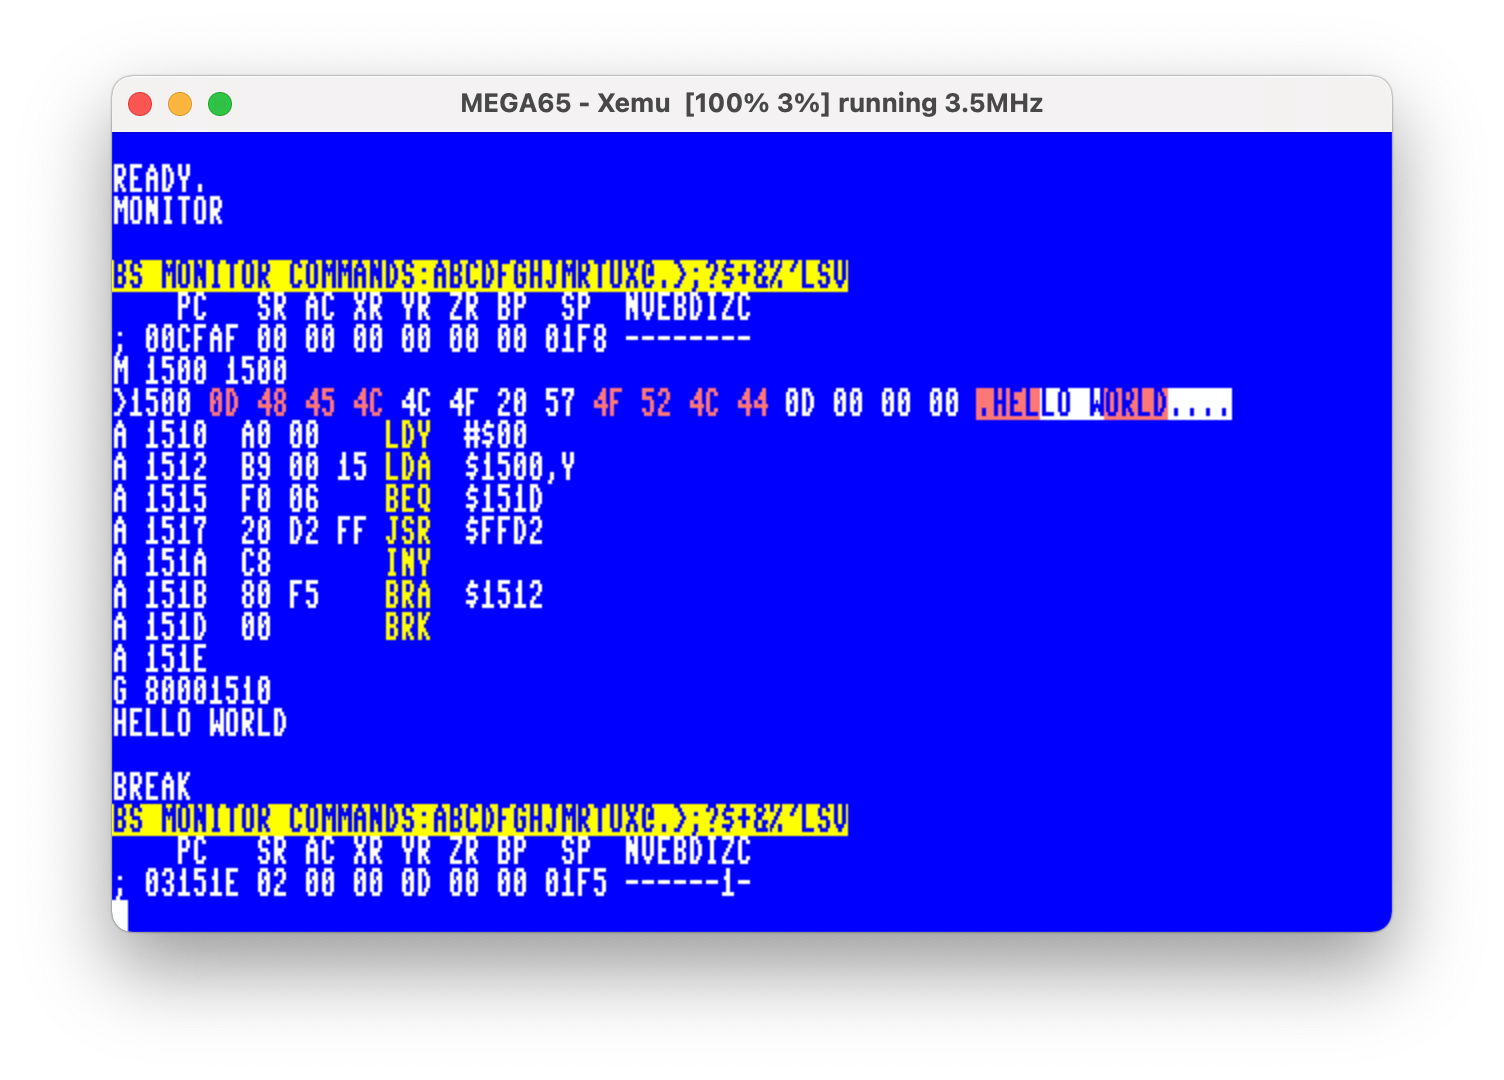
\includegraphics[width=\linewidth]{images/monitor-a}

% *******
% BITMAPS
% *******

\subsubsection{B : BITMAPS}

\index{BITMAPS}
\index{MONITOR-commando's!BITMAPS}
\begin{description}[leftmargin=2cm,style=nextline]
\item [Formaat:] {\bf B begin}\item [Gebruik:] Geeft geheugenwaarden weer, geïnterpreteerd als bitmaps van tekens.

\item [Opmerkingen:] Het commando B geeft de inhoud van geheugencellen bitsgewijs weer, waarbij voor een 1 een sterretje en voor een 0 een punt wordt afgedrukt. Daarbij wordt rekening gehouden met de bijzondere indeling van tekengegevens, waarbij 8 bytes samen één tekencel vormen. Bij elke aanroep worden 8 tekens weergegeven.

In de {\tt 92XXXX}-ROM's zijn drie ROM-tekensets ingebouwd:

\begin{tcolorbox}[colback=blue,coltext=white]
\verbatimfont{\codefont}
\begin{verbatim}
FONT A : REM $029000 : ASCII [\]^_ {|}~ inbegrepen
FONT B : REM $03D000 : versie van A met schreef
FONT C : REM $02D000 : origineel C64-lettertype
\end{verbatim}
\end{tcolorbox}
\end{description}
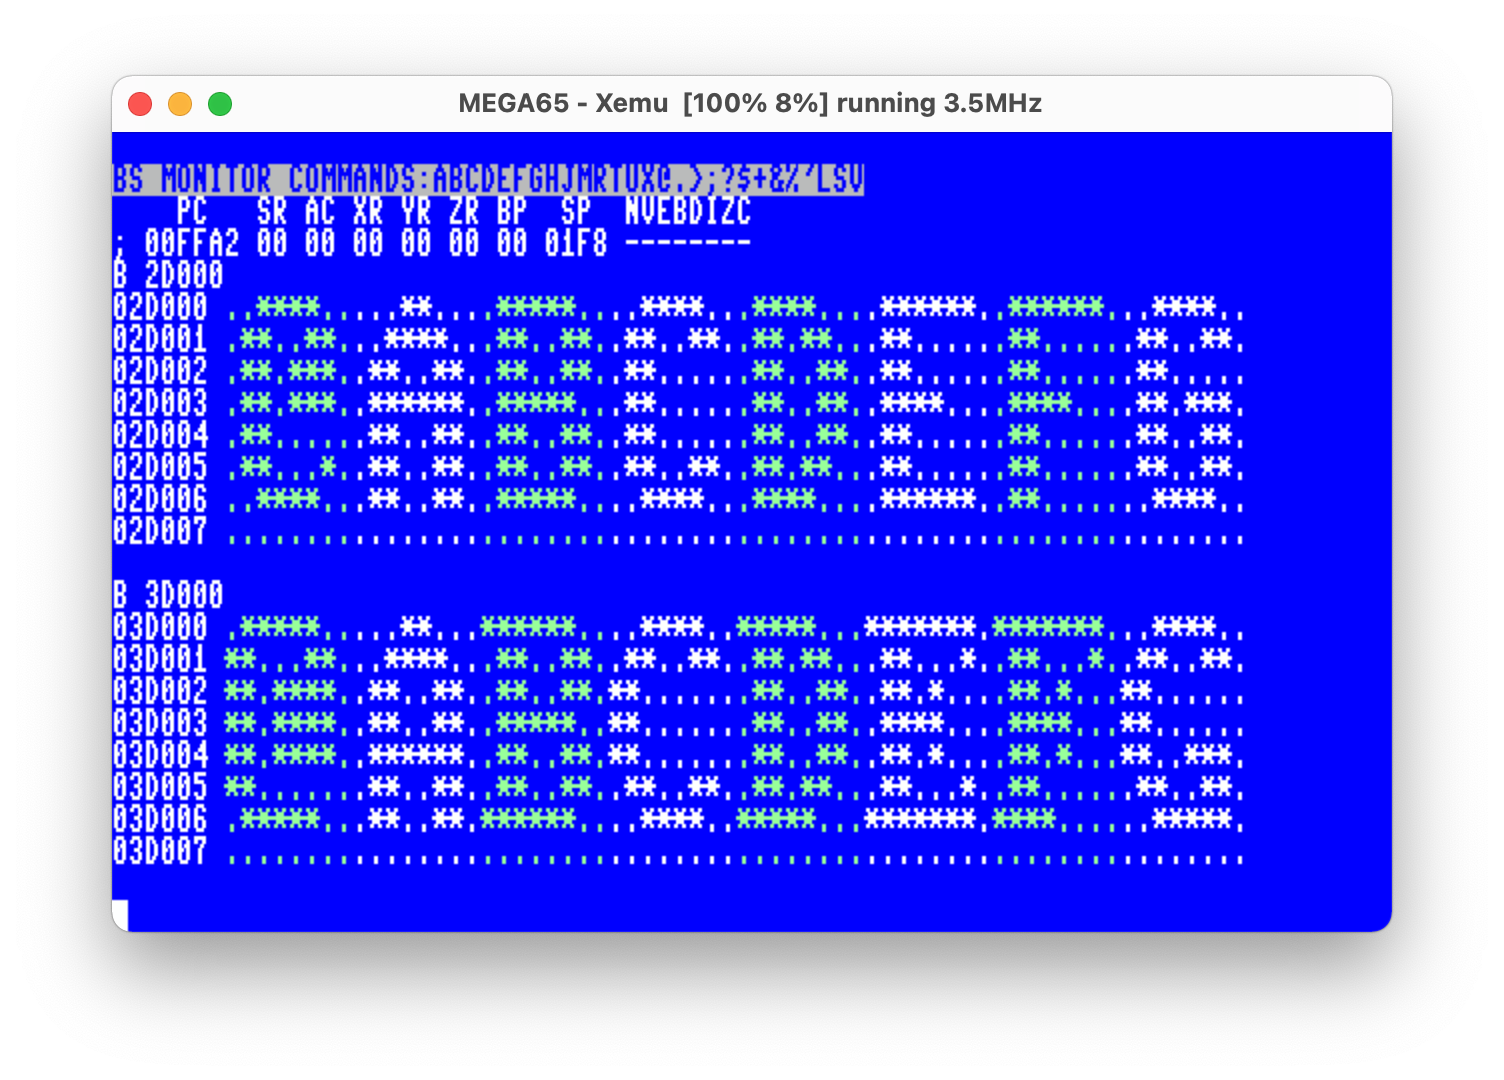
\includegraphics[width=\linewidth]{images/monitor-b}

% *******
% COMPARE
% *******

\subsubsection{C : COMPARE}
\index{COMPARE}
\index{MONITOR-commando's!COMPARE}
\begin{description}[leftmargin=2cm,style=nextline]
\item [Formaat:] {\bf C begin einde begin-b}\item [Gebruik:] Vergelijkt twee geheugengebieden en geeft vervolgens de adressen weer waarvan de waarden verschillen.

\item [Opmerkingen:] Het eindadres ligt één adres voorbij het laatste te vergelijken adres.

    Het tweede geheugengebied dat vergeleken wordt, begint op {\bf begin-b} en heeft dezelfde grootte als het gebied dat door {\bf begin} en {\bf einde} wordt omschreven.

    Adressen worden als hexadecimale waarden weergegeven.

\end{description}
% TODO: screenshot  \includegraphics[width=\linewidth]{images/monitor-c}

% ***********
% DISASSEMBLE
% ***********

\subsubsection{D : DISASSEMBLE}
\index{DISASSEMBLE}
\index{MONITOR-commando's!DISASSEMBLE}
\begin{description}[leftmargin=2cm,style=nextline]
\item [Formaat:] {\bf D [van [tot]]}\item [Gebruik:] Toont een listing in machinetaal voor het opgegeven adresbereik, in de veronderstelling dat het code bevat. Wanneer slechts één argument is opgegeven, disassembleert de disassembler de volgende 21 bytes. Indien geen argument is opgegeven, gaat de disassembly verder op het laatst gebruikte adres voor disassemblage. De inhoud wordt als hexadecimale waarden weergegeven.

\item [Opmerkingen:] De regels beginnen met het puntteken '.'. Hierdoor kunt u de disassembly direct op het volledige scherm bewerken. Drukt u in een willekeurige regel RETURN in, dan assembleert de monitor het gewijzigde commando van de cursorregel weer naar het geheugen, indien zich daar schrijfbare RAM bevindt. Zie het monitorcommando {\bf .}.

                 De disassembler kent de instructieset van de MEGA65-CPU, de
                 45GS02. Heeft een instructie het voorvoegsel {\bf NEG NEG}, dan worden
                 die hexadecimale waarden weggelaten en verschijnt in plaats daarvan
                 een sterretje ({\bf *}) tussen het adres en de hexadecimale waarden.

\item [Voorbeeld:] Gebruik van {\bf D}
\end{description}
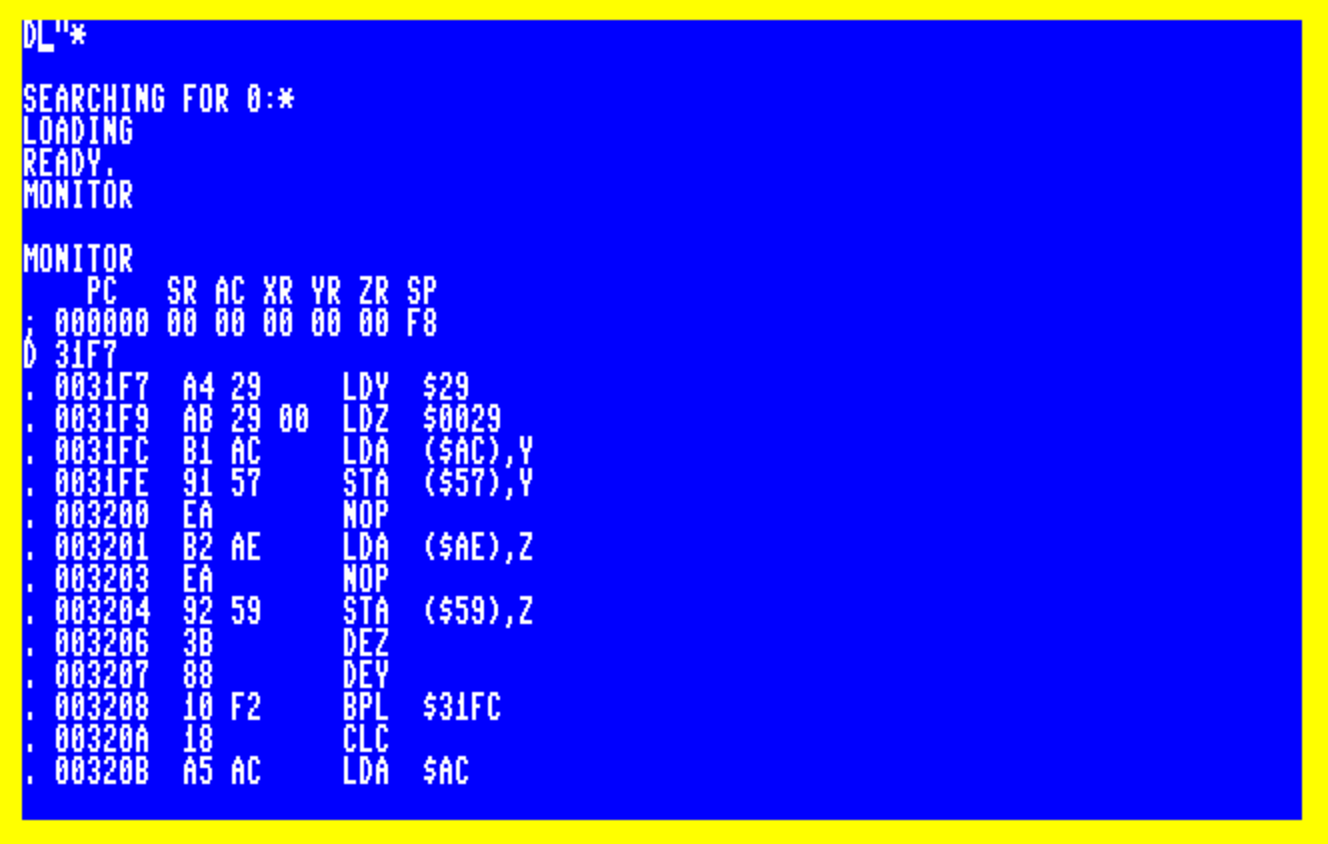
\includegraphics[width=\linewidth]{images/monitor-d}

% ****
% FILL
% ****

\subsubsection{F : FILL}
\index{FILL}
\index{MONITOR-commando's!FILL}
\begin{description}[leftmargin=2cm,style=nextline]
\item [Formaat:] {\bf F begin einde waarde}\item [Gebruik:] Vult een geheugengebied met een waarde.

\item [Opmerkingen:] Het eindadres ligt één adres voorbij het laatste adres dat gevuld wordt.
\end{description}
% TODO: screenshot  \includegraphics[width=\linewidth]{images/monitor-f}

% **
% GO
% **

\subsubsection{G : GO}
\index{GO}
\index{MONITOR-commando's!GO}
\begin{description}[leftmargin=2cm,style=nextline]
\item [Formaat:] {\bf G [adres]}\item [Gebruik:] Voert de code op een adres uit. Wordt {\bf adres} weggelaten, dan gebruikt de monitor de huidige programmateller als adres.

\item [Opmerkingen:] Dit is gelijkwaardig aan een {\bf JMP}-instructie.

    Het commando {\bf G} zonder argument is een handige manier om de uitvoering van een programma te hervatten nadat de monitor met een {\bf BRK}-instructie is gestart.

    Omdat dit een {\bf JMP} gebruikt, mag u dit commando niet gebruiken om subroutines aan te roepen. Zie {\bf J}.

\end{description}
% TODO: screenshot  \includegraphics[width=\linewidth]{images/monitor-g}

% ****
% HUNT
% ****

\subsubsection{H : HUNT}
\index{HUNT}
\index{MONITOR-commando's!HUNT}
\begin{description}[leftmargin=2cm,style=nextline]
\item [Formaat:] {\bf H begin einde byte [byte...]}\item [Gebruik:] Zoekt in een bereik van het geheugen naar elk voorkomen van een bytereeks en geeft vervolgens het beginadres van elk voorkomen weer.

\item [Opmerkingen:] Het eindadres ligt één adres voorbij het laatste adres dat doorzocht wordt.

    Adressen worden als hexadecimale waarden weergegeven.

\end{description}
% TODO: screenshot  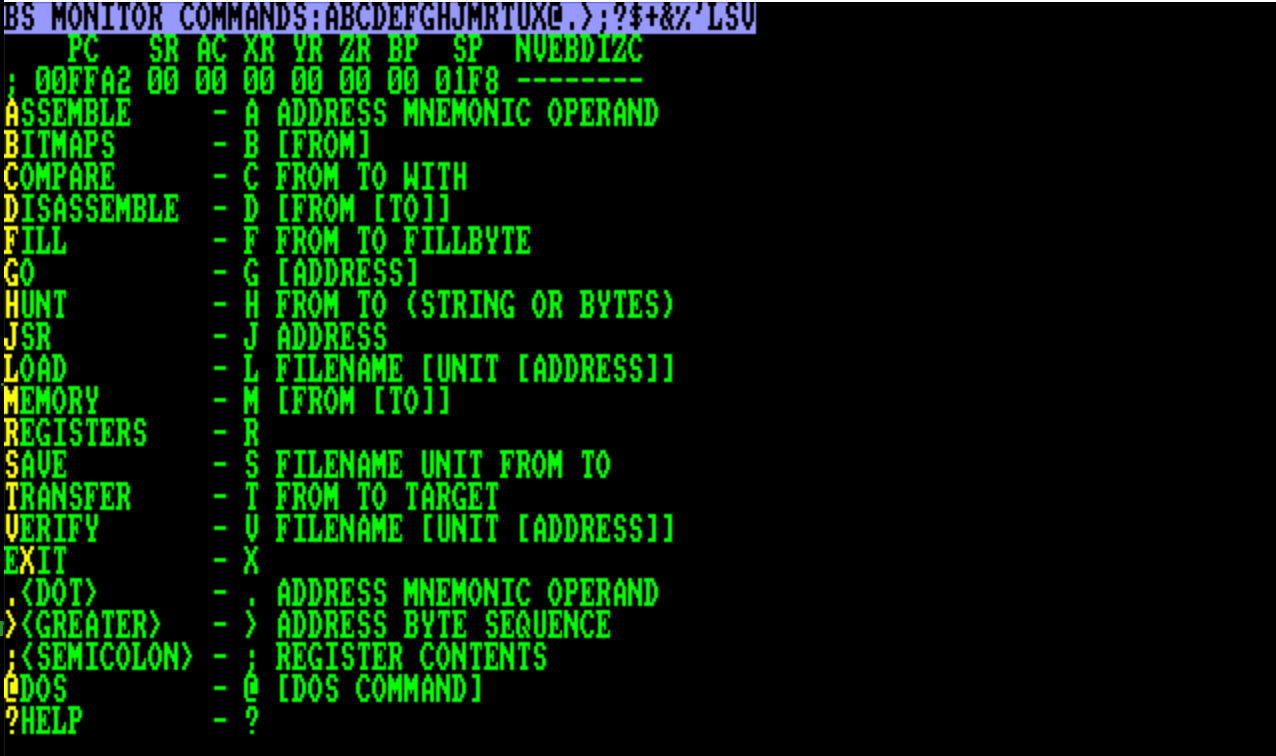
\includegraphics[width=\linewidth]{images/monitor-h}

% ****
% JUMP
% ****

\subsubsection{J : JUMP}
\index{JUMP}
\index{MONITOR-commando's!JUMP}
\begin{description}[leftmargin=2cm,style=nextline]
\item [Formaat:] {\bf J adres}\item [Gebruik:] Springt naar een subroutine op een adres.

\item [Opmerkingen:] Dit is gelijkwaardig aan een {\bf JSR}-instructie. Keert de subroutine terug met {\tt RTS}, dan neemt de monitor het weer over.

    Wilt u de uitvoering gewoon op een adres voortzetten zonder terugkeer naar de monitor te verwachten, gebruik dan {\bf G}.

\end{description}
% TODO: screenshot  \includegraphics[width=\linewidth]{images/monitor-j}

% ****
% LOAD
% ****

\subsubsection{L : LOAD}
\index{LOAD}
\index{MONITOR-commando's!LOAD}
\begin{description}[leftmargin=2cm,style=nextline]
\item [Formaat:] {\bf L "bestandsnaam",eenheid [begin]}\item [Gebruik:] Laadt gegevens uit een bestand in het geheugen.

\item [Opmerkingen:] De bestandsnaam moet tussen dubbele aanhalingstekens staan.

    Het nummer van de {\bf eenheid} (zoals 8 of 9) is verplicht. {\bf Eenheid} wordt opgegeven in het normale talstelsel van de monitor (standaard hexadecimaal). Zie \hyperref[sec:numbers]{Getallen}.

    Ontbreekt het {\bf begin}-adres, dan neemt de monitor het beginadres uit de eerste twee bytes van het bestand. Het bestand moet van het type {\tt PRG} zijn. Indien u {\bf begin} opgeeft, negeert de monitor de {\tt PRG}-kop van twee bytes.

\end{description}
% TODO: screenshot  \includegraphics[width=\linewidth]{images/monitor-l}

% ******
% MEMORY
% ******

\subsubsection{M : MEMORY}
\index{MEMORY}
\index{MONITOR-commando's!MEMORY}
\begin{description}[leftmargin=2cm,style=nextline]
\item [Formaat:] {\bf M [van [,tot]]}\item [Gebruik:] Drukt een geheugendump af voor het opgegeven adresbereik. De dump toont de geheugeninhoud, ingedeeld in rijen van 16 opeenvolgende adressen, te beginnen met het adres dat als eerste argument is opgegeven. De dump loopt door totdat een rij is afgedrukt die de waarde bevat van het adres dat als tweede argument is opgegeven. Ontbreekt het tweede argument, dan toont de dump een volledige pagina van 256 bytes in 16 rijen. De inhoud wordt afgedrukt als 16 bytewaarden in hexadecimale notatie, gevolgd door de tekenweergave.

\item [Opmerkingen:] De rijen beginnen met het teken '>'. Hierdoor kunt u de dump direct op het volledige scherm bewerken. Drukt u in een willekeurige rij RETURN in, dan schrijft de monitor de gewijzigde waarden van de cursorrij terug naar het geheugen, indien zich daar schrijfbare RAM bevindt. Zie het monitorcommando {\bf >}.

\item [Voorbeeld:] Gebruik van {\bf M}
\end{description}
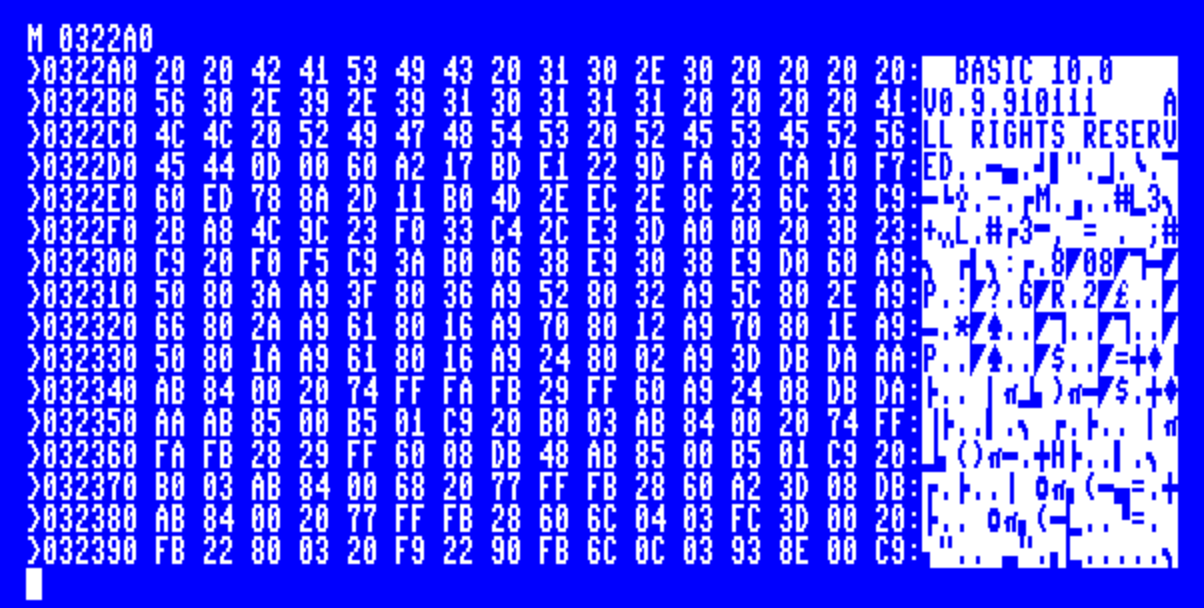
\includegraphics[width=\linewidth]{images/monitor-m}

% *********
% REGISTERS
% *********

\subsubsection{R : REGISTERS}
\index{REGISTERS}
\index{MONITOR-commando's!REGISTERS}
\begin{description}[leftmargin=2cm,style=nextline]
\item [Formaat:] {\bf R}\item [Gebruik:] Toont de inhoud van de registers zoals die waren vlak voordat de monitor werd gestart.

\item [Opmerkingen:] De uitvoer begint met het teken {\tt ;}, zodat u de registerwaarden kunt wijzigen door de cursor omhoog naar de regel te bewegen, de waarden aan te passen en vervolgens op \specialkey{RETURN} te drukken.

\end{description}
% TODO: screenshot  \includegraphics[width=\linewidth]{images/monitor-r}

% ****
% SAVE
% ****

\subsubsection{S : SAVE}
\index{SAVE}
\index{MONITOR-commando's!SAVE}
\begin{description}[leftmargin=2cm,style=nextline]
\item [Formaat:] {\bf S "bestandsnaam",eenheid begin einde}\item [Gebruik:] Slaat een geheugengebied op in een bestand op schijf, van het type {\tt PRG}.

\item [Opmerkingen:] De bestandsnaam moet tussen dubbele aanhalingstekens staan.

    Het nummer van de {\bf eenheid} (zoals 8 of 9) is verplicht. {\bf Eenheid} wordt opgegeven in het normale talstelsel van de monitor (standaard hexadecimaal). Zie \hyperref[sec:numbers]{Getallen}.

    Het eindadres ligt één adres voorbij het laatste adres dat opgeslagen wordt.

    Om een bestaand bestand te overschrijven, plaatst u {\tt 0:} vóór de bestandsnaam, bijvoorbeeld: {\tt "0:MYFILE"}.

\end{description}
% TODO: screenshot  \includegraphics[width=\linewidth]{images/monitor-s}

% ********
% TRANSFER
% ********

\subsubsection{T : TRANSFER}
\index{TRANSFER}
\index{MONITOR-commando's!TRANSFER}
\begin{description}[leftmargin=2cm,style=nextline]
\item [Formaat:] {\bf T begin einde bestemmingsbegin}\item [Gebruik:] Kopieert een geheugengebied naar een ander gebied.

\item [Opmerkingen:] Het eindadres ligt één adres voorbij het laatste adres dat gekopieerd wordt.

    De monitor veronderstelt dat het doelgebied even lang is als het brongebied. Alle bytes worden gekopieerd.

\end{description}
% TODO: screenshot  \includegraphics[width=\linewidth]{images/monitor-t}

% ******
% VERIFY
% ******

\subsubsection{V : VERIFY}
\index{VERIFY}
\index{MONITOR-commando's!VERIFY}
\begin{description}[leftmargin=2cm,style=nextline]
\item [Formaat:] {\bf V "bestandsnaam",eenheid begin}\item [Gebruik:] Controleert of een geheugengebied overeenkomt met een bestand op schijf.

\item [Opmerkingen:] De bestandsnaam moet tussen dubbele aanhalingstekens staan.

    Het nummer van de {\bf eenheid} (zoals 8 of 9) is verplicht. {\bf Eenheid} wordt opgegeven in het normale talstelsel van de monitor (standaard hexadecimaal). Zie \hyperref[sec:numbers]{Getallen}.

    De monitor veronderstelt dat de te controleren gegevens even lang zijn als het bestand.

    Komen de gegevens in het geheugen niet overeen, dan toont de monitor een foutmelding. Anders verschijnt er niets meer en kunt u ervan uitgaan dat de controle is geslaagd.

\end{description}
% TODO: screenshot  \includegraphics[width=\linewidth]{images/monitor-v}

% ****
% EXIT
% ****

\subsubsection{X : EXIT}
\index{EXIT}
\index{MONITOR-commando's!EXIT}
\begin{description}[leftmargin=2cm,style=nextline]
\item [Formaat:] {\bf X}\item [Gebruik:] Verlaat de monitor en keert terug naar BASIC.

\item [Opmerkingen:] Indien de monitor werd gestart door een {\bf BRK}-instructie in een programma, betekent het verlaten van de monitor in feite dat het programma wordt afgebroken. Om een gepauzeerd programma voort te zetten, gebruikt u in plaats daarvan {\bf G}.

\end{description}

% ************
% . (ASSEMBLE)
% ************

\subsubsection{. : ASSEMBLE}
\index{MONITOR-commando's!.}
\begin{description}[leftmargin=2cm,style=nextline]
\item [Formaat:] {\bf . adres opcode operand}\item [Gebruik:] Een alias voor {\bf A}.

\item [Opmerkingen:] De uitvoer van de disassembler begint elke regel met het teken {\tt .}. U kunt de door de disassembler afgedrukte machinetaalinstructies bewerken door de cursor omhoog naar een regel te bewegen, de regel aan te passen en vervolgens op \specialkey{RETURN} te drukken. Hierdoor verandert het {\tt .} in een {\tt A}, zodat u kunt zien welke regels opnieuw zijn geassembleerd.

\end{description}
% TODO: screenshot  \includegraphics[width=\linewidth]{images/monitor-dot}

% *****************
% > (MODIFY MEMORY)
% *****************

\subsubsection{> : MODIFY MEMORY}
\index{MONITOR-commando's!>}
\begin{description}[leftmargin=2cm,style=nextline]
\item [Formaat:] {\bf > adres byte [byte...]}\item [Gebruik:] Wijzigt één of meer bytes vanaf een adres.

\item [Opmerkingen:] De uitvoer van het commando {\bf M} begint elke regel met het teken {\tt >}. U kunt de door het commando {\bf M} afgedrukte geheugenwaarden bewerken door de cursor omhoog naar een regel te bewegen, de regel aan te passen en vervolgens op \specialkey{RETURN} te drukken.

\end{description}
% TODO: screenshot  \includegraphics[width=\linewidth]{images/monitor-gt}

% ********************
% ; (MODIFY REGISTERS)
% ********************

\subsubsection{; : MODIFY REGISTERS}
\index{MONITOR-commando's!.}
\begin{description}[leftmargin=2cm,style=nextline]
\item [Formaat:] {\bf ; pc sr ac xr yr zr bp sp nvebdizc}\item [Gebruik:] Wijzigt de CPU-registers. De argumenten hebben dezelfde indeling als de uitvoer van het commando {\bf R}.

\item [Opmerkingen:] De uitvoer van het commando {\bf R} begint de regel met het teken {\tt ;}. U kunt de door het commando {\bf R} afgedrukte registerwaarden bewerken door de cursor omhoog naar de regel te bewegen, de regel aan te passen en vervolgens op \specialkey{RETURN} te drukken.

\end{description}
% TODO: screenshot  \includegraphics[width=\linewidth]{images/monitor-semi}

% ****************
% @ (DISK COMMAND)
% ****************

\subsubsection{@ : DISK COMMAND}
\index{MONITOR-commando's!@}
\begin{description}[leftmargin=2cm,style=nextline]
\item [Formaat:] {\bf @ [eenheid] [,commando]}\item [Gebruik:] Voert een schijfcommando uit.

\item [Opmerkingen:] Zonder {\bf commando} toont dit de status van het schijfstation.

    Standaard is de {\bf eenheid} 8. De {\bf eenheid} wordt opgegeven in het normale talstelsel van de monitor (standaard hexadecimaal). Zie \hyperref[sec:numbers]{Getallen}.

    Een {\bf commando} van {\bf \$[pattern]} vraagt bij de opgegeven {\bf eenheid} een directoryoverzicht op en toont dit. U kunt optioneel een {\bf patroon} opgeven om de getoonde bestanden te beperken. De jokertekens {\bf *} en {\bf ?} kunnen worden gebruikt

    Het {\bf commando} kan elk Commodore-DOS-commando zijn. Om bijvoorbeeld een bestand te hernoemen: {\tt @R0:NEWNAME=OLDNAME}

    Het {\bf commando} kan {\tt U1} zijn om ruwe schijfsectoren naar het geheugen te lezen, of {\tt U2} om geheugen naar ruwe schijfsectoren weg te schrijven. Deze {\bf commando's} hebben de volgende vorm:

    {\bf @8,U1 geheugenbegin track sector [sectoraantal]}

    De tracks zijn genummerd van 1 tot 80 en de sectoren van 0 tot 39. Wordt {\bf sectoraantal} weggelaten, dan wordt slechts één sector gelezen of geschreven.

\end{description}
% TODO: screenshot  \includegraphics[width=\linewidth]{images/monitor-at}



\section{De Matrix Mode/seriële monitor}
\label{sec:matrix-mode}
\index{MONITOR!Matrix Mode/seriële monitor}

De Matrix Mode-monitor kan iets wat de MEGA65-monitor niet kan: in plaats van een programma te pauzeren om de monitor te draaien, draait de Matrix Mode-monitor gelijktijdig met het actieve programma mee. Dat houdt in dat u het geheugen van de MEGA65 kunt bekijken en wijzigen, {\em terwijl een programma wordt uitgevoerd}.

Dit werkt dankzij speciale hardware in het ontwerp van de MEGA65, waarin een kleine hulpprocessor is opgenomen die deze monitorinterface draait. Deze hardware heeft een speciaal toegangsmechanisme voor het geheugen en de CPU van de MEGA65.

In vergelijking met de monitors in de ROM, die op de hoofdprocessor van de MEGA65 draaien, heeft de Matrix Mode-monitor een aantal voor- en nadelen:
\begin{itemize}
\item Hij kan worden gebruikt terwijl een programma draait.\item Hij kan worden gebruikt, zelfs wanneer het ROM-gebied voor programmacode of gegevens wordt gebruikt in plaats van een standaard C65- of MEGA65-ROM te bevatten.\item Hij is bereikbaar via de seriële debug-interface op de JB1-connector.\item Hij kan worden opgedragen de processor te stoppen zodra het programmatellerregister (PC) van de hoofdprocessor een door de gebruiker opgegeven adres bereikt. Dat wil zeggen dat hij één hardware-breakpoint ondersteunt.\item Hij kan worden opgedragen de processor te stoppen telkens wanneer naar een opgegeven geheugenadres wordt geschreven. Dat wil zeggen dat hij een ``write watch'' op één geheugenadres ondersteunt. Het geheugenadres wordt opgegeven als een volledig 28-bits adres, zodat hij geheugenschrijfbewerkingen via elke denkbare weg kan detecteren. Let op: lopende DMA-bewerkingen worden nog voltooid voordat het watchpoint ingaat.\item Hij kan worden opgedragen de processor te stoppen telkens wanneer specifieke CPU-vlaggen worden gezet of gewist, wat ook kan worden gebruikt om het debuggen van programma's te ondersteunen.\item Op sommige modellen van de MEGA65 is de ingebouwde ROM van de monitorprocessor zeer klein, waardoor de functionaliteit beperkt kan zijn. Deze monitor kent bijvoorbeeld geen ``assemble''-commando. Dat kan in toekomstige core-updates worden verholpen voor MEGA65-modellen waarvan de monitorprocessor ruimte biedt voor een grotere ROM.
\end{itemize}

\subsection{Tabel met Matrix Mode-mon\-itorcom\-mando's}

{
\ttfamily
\setlength{\tabcolsep}{1mm}
\begin{center}
\begin{tabular}{|l|l|L{6.5cm}|}
\hline
C & mnemoniek & beschrijving \\
\hline
<Enter> & STEP & Voert de volgende instructie uit \\\# & HYPERTRAP & Schakelt CPU-hypervisor-traps in of uit \\+ & UARTDIVISOR & Stelt de UART-baudratedeler in \\? & HELP & Hulp \\@ & CPUMEM & (toont geheugen vanuit de CPU-context) \\
\hline
B & BREAKPOINT & Stelt het breakpoint voor de CPU-uitvoering in of wist het \\D & DISASSEMBLE & Disassembleert het geheugen \\E & FLAGWATCH & Stelt het watchpoint voor de CPU-vlaggen in of wist het \\F & FILL & Vult een geheugengebied met een waarde \\G & SETPC & Stelt de programmateller van de CPU in \\H & HELP & hulp \\I & INTERRUPTS & Schakelt CPU-IRQ's in of uit (wist/zet de I-vlag van de CPU) \\J & DEBUGMON & Diverse debugfuncties voor de monitor zelf \\L & LOADMEMORY & Laadt gegevens in het geheugen \\M & MEMORY & Toont de geheugeninhoud \\R & REGISTERS & Toont de registers \\S & SETMEMORY & Stelt de geheugeninhoud in \\T & TRACE & stelt de traceer- of uitvoeringsmodus van de CPU in \\W & MEMORYWATCH & Stelt het watchpoint voor geheugenschrijfacties in of wist het \\Z & CPUHISTORY & CPU-geschiedenis \\
\hline
\end{tabular}
\end{center}
}

\subsection {De monitor aanroepen}

Om de monitor te openen of te verlaten houdt u \megasymbolkey ingedrukt en drukt u op \specialkey{TAB}. U ziet een animatie van groene tekens die als een regen vanaf de bovenkant van het scherm naar beneden vallen, waarna u een eenvoudige tekstterminal-interface aangeboden krijgt. Die is transparant, zodat u tegelijkertijd de schermuitvoer van uw draaiende programma kunt zien.

\subsubsection{<Enter> : Single-step}

\index{STEP}
\index{MONITOR-commando's!STEP}
\begin{description}[leftmargin=2cm,style=nextline]
\item [Formaat:] {\bf <Enter-toets> Voert de volgende instructie uit}\item [Gebruik:] <Enter-toets>\item [Opmerkingen:] Bevindt de CPU zich in de trace-modus {\bf t1}, dan voert het indrukken van de Enter- (of Return-)toets bij de prompt zonder commando de volgende CPU-instructie uit en verhoogt de programmateller. Zie hieronder bij ``Trace''.
\end{description}


\subsubsection{\# : Hypervisor-trap in-/uitschakelen}

\index{HYPERTRAP}
\index{MONITOR-commando's!HYPERTRAP}
\begin{description}[leftmargin=2cm,style=nextline]
\item [Formaat:] {\bf \# Schakelt hypervisor-traps in of uit}\item [Gebruik:] \#[0|1]

\item [Opmerkingen:] Is het argument 1, dan worden de hypervisor-traps ingeschakeld; in het andere geval worden ze uitgeschakeld.

  {\em Het is niet bevestigd of dit commando momenteel functioneert.}
\end{description}


\subsubsection{+ : Stel UART-baudratedeler seriële interface in}

\index{UARTDIVISOR}
\index{MONITOR-commando's!UARTDIVISOR}
\begin{description}[leftmargin=2cm,style=nextline]
\item [Formaat:] {\bf + Stelt de UART-baudratedeler van de seriële interface in}\item [Gebruik:] + deler

\item [Opmerkingen:] Stelt de deler voor de seriële monitorinterface in. Met dit commando kunt u de baudrate van de seriële monitorinterface wijzigen ten opzichte van de standaardwaarde van 2000000 bits per seconde. De baudrate bedraagt $40,500,000 \div (divisor-1)$. Dit heeft alleen betrekking op de seriële UART-interface en verandert niets aan de toegang tot deze monitor via de samengestelde weergave van Matrix Mode.

  Wilt u de seriële monitorinterface bijvoorbeeld vertragen naar 19200 bits per seconde, dan moet de deler $40,500,000 \div (19,200 - 1) = 2108$ zijn. Het commando + vereist vervolgens dat u deze waarde naar hexadecimaal omrekent; het commando luidt dan {\tt +83c}.

  Let op: dit commando controleert de opgegeven waarde {\em niet} op geldigheid. Geeft u per ongeluk een voor uw doeleinden onjuiste waarde op, dan kunt u dit herstellen door de Matrix Mode-interface te activeren: houd \megasymbolkey ingedrukt en tik op \specialkey{TAB}, en geef daarna het juiste commando om de deler te corrigeren, bijvoorbeeld {\tt +14} om terug te keren naar de standaardwaarde van 2000000 bits per seconde.

  Vervolgens moet u Matrix Mode weer verlaten door de toetsencombinatie \megasymbolkey + \specialkey{TAB} te herhalen, voordat de seriële UART-interface weer actief wordt. Dat komt doordat Matrix Mode de seriële UART-interface uitschakelt zolang de modus actief is.
\end{description}

\subsubsection{@ : CPUMEMORY}
\index{CPUMEMORY}
\index{MONITOR-commando's!CPUMEMORY}
\begin{description}[leftmargin=2cm,style=nextline]
\item [Formaat:] {\bf @ [adres]}\item [Gebruik:] Drukt een geheugendump af voor het opgegeven 16-bits adres, {\em zoals geïnterpreteerd door de huidige geheugenmapping van de CPU}. Wilt u de inhoud van het geheugen ergens in de 28-bits adresruimte bekijken, gebruik dan in plaats daarvan het commando M.

  De dump toont de geheugeninhoud, ingedeeld in rijen van 16 opeenvolgende adressen, te beginnen met het opgegeven adres. De dump toont een volledige pagina van 256 bytes in 16 rijen. De inhoud wordt afgedrukt als 16 bytewaarden in hexadecimale notatie, gevolgd door de tekenweergave.

\item [Opmerkingen:] Ontbreekt een adres, dan toont de monitor de volgende 256 bytes.

\end{description}

\subsubsection{? of H : HELP}
\index{HELP}
\index{MONITOR-commando's!HELP}
\begin{description}[leftmargin=2cm,style=nextline]
\item [Formaat:] {\bf ?} {\em of} {\bf h}\item [Gebruik:] Toont een (zeer) korte melding die de monitor identificeert. Op sommige MEGA65-modellen waarvoor meer geheugen beschikbaar is voor de monitorprocessor kan dit commando informatie over elk van de beschikbare commando's weergeven.

\end{description}


\subsubsection{B : BREAKPOINT}
\index{BREAKPOINT}
\index{MONITOR-commando's!BREAKPOINT}
\begin{description}[leftmargin=2cm,style=nextline]
\item [Formaat:] {\bf b [adres]}\item [Gebruik:] Stelt het hardware-breakpoint in of wist het. Indien geen adres is opgegeven, wordt het breakpoint uitgeschakeld. Anders wordt het breakpoint ingesteld op het opgegeven 16-bits adres.

  Zodra het programmatellerregister (PC) van de processor van de MEGA65 gelijk is aan de waarde die bij dit commando is opgegeven, stopt de processor en toont de Matrix Mode-monitorinterface de laatst uitgevoerde instructie en de huidige registerwaarden, om u op deze gebeurtenis te wijzen. Hierbij wordt de Matrix Mode-weergave niet geactiveerd. Er wordt normaliter van uitgegaan dat de Matrix Mode al actief is of dat u via de seriële interface communiceert.

\end{description}


\subsubsection{D : DISASSEMBLE}
\index{DISASSEMBLE}
\index{MONITOR-commando's!DISASSEMBLE}
\begin{description}[leftmargin=2cm,style=nextline]
\item [Formaat:] {\bf <d|D> [adres]}\item [Gebruik:] Disassembleert de instructie op het opgegeven 28-bits adres en geeft deze weer.

  Om instructies te disassembleren vanuit de huidige geheugencontext van de CPU, met inachtneming van de huidige geheugenbanking, plaatst u 777 vóór het adres. Zo disassembleert {\tt d777080D} bijvoorbeeld de instructie op \$080D, zoals die momenteel zichtbaar is voor de processor van de MEGA65.

  Met {\tt D} in plaats van {\tt d} disassembleert u per keer 16 instructies in plaats van slechts één.

\end{description}

\subsubsection{E : FLAGWATCH}
\index{FLAGWATCH}
\index{MONITOR-commando's!FLAGWATCH}
\begin{description}[leftmargin=2cm,style=nextline]
\item [Formaat:] {\bf e [waarde]}\item [Gebruik:] Stelt het watchpoint voor CPU-vlaggen in of wist dit: Indien geen argument is opgegeven, wordt het watchpoint uitgeschakeld. Indien een waarde is opgegeven, wordt deze als 16-bits waarde opgevat, waarbij de eerste twee hexadecimale cijfers aangeven welke processorvlaggen het watchpoint activeren indien zij gezet zijn. De laatste twee hexadecimale cijfers geven aan welke processorvlaggen het watchpoint activeren indien zij gewist zijn. Op deze manier kunt u elke combinatie van processorvlagwaarden bewaken.

  {\em Dit commando functioneert ten tijde van het schrijven van deze handleiding niet correct.}

\item [Voorbeeld:]

  Om het watchpoint te laten afgaan wanneer de N-vlag is gezet, gebruikt u het commando {\tt e8000}.

\end{description}

\subsubsection{F : FILL}
\index{FILL}
\index{MONITOR-commando's!FILL}
\begin{description}[leftmargin=2cm,style=nextline]
\item [Formaat:] {\bf f [begin] [einde+1] [waarde] }\item [Gebruik:] Vult het opgegeven 28-bits adresbereik met de opgegeven waarde.\item [Opmerkingen:] Het eindadres moet één adres voorbij het laatste adres liggen dat u wilt vullen.

\end{description}

\subsubsection{G : SETPC}
\index{SETPC}
\index{MONITOR-commando's!SETPC}
\begin{description}[leftmargin=2cm,style=nextline]
\item [Formaat:] {\bf g adres}\item [Gebruik:] Stelt het programmatellerregister (PC) van de processor van de MEGA65 in op het opgegeven 16-bits adres. Draait de processor op dat moment, dan gaat de uitvoering onmiddellijk vanaf dat adres verder. Is de processor op dat moment gestopt, bijvoorbeeld doordat het commando {\tt t1} is gebruikt, dan blijft hij stopgezet, met de programmateller ingesteld op het opgegeven adres, gereed voor het moment waarop de processor weer mag draaien.

\end{description}


\subsubsection{I : INTERRUPTS}
\index{INTERRUPTS}
\index{MONITOR-commando's!INTERRUPTS}
\begin{description}[leftmargin=2cm,style=nextline]
\item [Formaat:] {\bf i[0|1]}\item [Gebruik:] Schakelt interruptverzoeken (IRQ's) van de processor van de MEGA65 in of uit. Het uitschakelen van IRQ's kan nuttig zijn wanneer u een programma instructie voor instructie doorloopt: anders loopt u doorgaans uitsluitend door de code van de interruptafhandelaar, omdat interrupts vaker optreden dan uw stappen door de code.

  {\bf i1} zet de CPU-vlag ``IRQs disabled'' (I). De CPU reageert daardoor niet langer op IRQ-bronnen, zoals CIA-timers of rasterstraalbewakingen van de VIC. Dit schakelt non-maskable interrupts (NMI's) niet uit. Er bestaat geen manier om NMI's uit te schakelen vanuit de seriële debugger (of vanuit een programma).

  {\bf i0} wist de I-vlag van de CPU. Dit schakelt de IRQ's weer in.

\item [Opmerkingen:] Als de CPU door {\bf t1} is stopgezet, toont het registeroverzicht ({\bf r}) de gewijzigde I-vlag pas nadat de volgende instructie is uitgevoerd.

\end{description}

\subsubsection{J : DEBUGMON}
\index{DEBUGMON}
\index{MONITOR-commando's!DEBUGMON}
\begin{description}[leftmargin=2cm,style=nextline]
\item [Formaat:] {\bf j [waarde]}\item [Gebruik:] Toont interne signalen van de Matrix Mode-monitorinterface en stelt die desgewenst in.

\end{description}


\subsubsection{L : LOADMEMORY}
\index{LOADMEMORY}
\index{MONITOR-commando's!LOADMEMORY}
\begin{description}[leftmargin=2cm,style=nextline]
\item [Formaat:] {\bf l <beginadres> <eindadres + 1>}\item [Gebruik:] Laadt een geheugenblok snel in via de seriële monitorinterface. Onmiddellijk nadat u dit commando heeft verstuurd, moet u de te laden geheugenbytes naar de seriële monitorinterface sturen. De bytes worden ongewijzigd ingelezen en moeten derhalve als gewone bytes worden aangeboden, niet hexadecimaal gecodeerd. Hiermee laadt u gegevens met een snelheid van circa 200KB per seconde bij de standaard seriële baudrate van 2000000 bits per seconde.

\end{description}

\subsubsection{M : MEMORY}
\index{MEMORY}
\index{MONITOR-commando's!MEMORY}
\begin{description}[leftmargin=2cm,style=nextline]
\item [Formaat:] {\bf <m|M> [adres]}\item [Gebruik:] Drukt een geheugendump af voor het opgegeven 28-bits adres. Wilt u de inhoud van het geheugen bekijken zoals de processor die op dit moment ziet met de huidige instellingen voor geheugenbanking, gebruik dan in plaats daarvan het commando {\bf @}.

  De dump toont de geheugeninhoud, ingedeeld in rijen van 16 opeenvolgende adressen, te beginnen met het opgegeven adres. De dump toont een volledige pagina van 256 bytes in 16 rijen. De inhoud wordt afgedrukt als 16 bytewaarden in hexadecimale notatie, gevolgd door de tekenweergave.

  Om het geheugen te bekijken vanuit de huidige geheugencontext van de CPU, waarbij rekening wordt gehouden met de huidige geheugenbanking, plaatst u 777 vóór het adres; met {\tt m777080D} bekijkt u bijvoorbeeld het geheugen op \$080D, zoals dat op dat moment zichtbaar is voor de processor van de MEGA65.


\item [Opmerkingen:] Is er geen adres opgegeven, dan toont de monitor de volgende 256 bytes.

\end{description}

\subsubsection{R : REGISTERS}
\index{REGISTERS}
\index{MONITOR-commando's!REGISTERS}
\begin{description}[leftmargin=2cm,style=nextline]
\item [Formaat:] {\bf r}\item [Gebruik:] Toont de huidige waarde van verschillende processorregisters en -vlaggen, alsmede een disassembly van de meest recent uitgevoerde instructie.

\end{description}

\subsubsection{S : SETMEMORY}
\index{SETMEMORY}
\index{MONITOR-commando's!SETMEMORY}
\begin{description}[leftmargin=2cm,style=nextline]
\item [Formaat:] {\bf s adres <waarde ...>}\item [Gebruik:] Stelt de inhoud van de opgegeven geheugenlocatie in op de aangeleverde waarde. Geeft u meer dan één door spaties gescheiden waarde op, dan worden meerdere opeenvolgende geheugenlocaties ingesteld.

  Dit commando gebruikt 28-bits adressen en negeert derhalve de momenteel geselecteerde instellingen voor geheugenbanking.

\end{description}


\subsubsection{T : TRACE}
\index{TRACE}
\index{MONITOR-commando's!TRACE}
\begin{description}[leftmargin=2cm,style=nextline]
\item [Formaat:] {\bf t<0|1|c>}\item [Gebruik:] Kiest de traceer- of uitvoeringsmodus van de processor: {\tt t0} betekent dat de processor vrij draait, {\tt t1} stopt de processor, en {\tt tc} laat de processor in de doorlopende traceermodus draaien, waarbij elke instructie en de registerwaarden onmiddellijk na de uitvoering worden weergegeven, alsof {\tt t1} was gekozen en de gebruiker daarna onmiddellijk op Return of Enter zou drukken om de uitvoering van de volgende instructie te vragen.

  Is {\tt t1} gekozen, dan wordt in de Matrix Mode-monitor de volgende instructie uitgevoerd zodra u op Enter of Return drukt.

  Het commando {\tt t0} wordt ook gebruikt nadat een breakpoint of watchpoint is afgegaan, zodat de processor de uitvoering kan hervatten.

\end{description}

\subsubsection{W : WATCHPOINT}
\index{WATCHPOINT}
\index{MONITOR-commando's!WATCHPOINT}
\begin{description}[leftmargin=2cm,style=nextline]
\item [Formaat:] {\bf w [adres]}\item [Gebruik:] Stelt het hardware-watchpoint in of wist het. Is er geen adres opgegeven, dan wordt het watchpoint uitgeschakeld. In het andere geval wordt het watchpoint ingesteld op het opgegeven 28-bits adres.

  Zodra de processor van de MEGA65 naar het adres schrijft dat aan dit commando is meegegeven, stopt de processor en toont de Matrix Mode-monitorinterface de laatst uitgevoerde instructie en de huidige registerwaarden om u op deze gebeurtenis te wijzen. Hierbij wordt de Matrix Mode-weergave niet geactiveerd. Er wordt normaliter van uitgegaan dat de Matrix Mode al actief is, of dat u via de seriële interface communiceert.

\end{description}

\subsubsection{Z : CPUHISTORY}
\index{CPUHISTORY}
\index{MONITOR-commando's!CPUHISTORY}
\begin{description}[leftmargin=2cm,style=nextline]
\item [Formaat:] {\bf z [adres]}\item [Gebruik:] Toont informatie over de instructies die de processor van de MEGA65 onlangs heeft uitgevoerd.

\item [Opmerkingen:] {\em Er wordt vermoed dat dit commando op het moment van schrijven niet correct functioneert.}

\end{description}





% The local subsubsection restyle above is meant for this appendix only.
% \titleformat* is document-wide; restore the class default so that it
% does not leak into the appendices that follow.
\titleformat*{\subsubsection}{\normalfont\normalsize\bfseries}

  \chapter{F018-compatibele controller voor Direct Memory Access (DMA)}
\label{cha:dmagic}

De MEGA65 bevat een F018/F018A-compatibele DMA-controller. Anders dan in de C65, waar de DMA-controller als een afzonderlijke chip bestaat, maakt deze in de MEGA65 deel uit van de 45GS02-processor. Omdat het gebruik van de DMA-controller echter een logisch afzonderlijk onderwerp vormt, wordt het apart in deze bijlage besproken.

De DMA-controller van de MEGA65 biedt diverse belangrijke verbeteringen ten opzichte van de F018/F018A-DMAgic-chips van de C65:

\begin{itemize}
\item{\bf Snelheid} De MEGA65 voert DMA-bewerkingen uit met 40 MHz, waardoor per seconde 40 MB kan worden gevuld of 20 MB kan worden gekopieerd. Zo is het bijvoorbeeld mogelijk om een volledige bitmapafbeelding van 8 KB in C64-stijl in circa 200 microseconden te kopiëren, wat overeenkomt met minder dan vier rasterlijnen! \item{\bf Toegang tot het volledige geheugen} De DMA-controller van de MEGA65 biedt toegang tot alle 256 MB van de adresruimte. \item{\bf Ondersteuning voor het kopiëren van texturen} De DMA-controller van de MEGA65 kan fractionele adresberekeningen uitvoeren ter ondersteuning van hardwarematige textuurschaling, evenals adresstriding, waardoor het in principe mogelijk is om een textuur gelijktijdig te schalen en vanuit het geheugen naar het scherm te tekenen. Dat zou nuttig zijn als iemand gek genoeg zou zijn om een spel in de stijl van Wolfenstein of Doom op de MEGA65 te implementeren. \item{\bf Ondersteuning voor transparantie- en maskerwaarden} De DMA-controller van de MEGA65 kan de opdracht krijgen om bij het kopiëren van geheugen een speciale waarde te negeren, waardoor de inhoud van het bestemmingsgeheugen ongewijzigd blijft. Dit maakt het maskeren van transparante gebieden bij een DMA-kopie mogelijk, wat het blitten van grafische vormen aanzienlijk vereenvoudigt. \item{\bf Optielijst per taak} Voor elke taak in een geketende lijst van DMA-taken kunnen diverse opties worden geconfigureerd, zoals het selecteren van de F018- of F018B-modus, het wijzigen van de transparantiewaarde, fractionele adresstappen of het bron- of bestemmingsgeheugengebied.

\item{\bf Achtergrond-audio-DMA}  De MEGA65 beschikt over mogelijkheden voor achtergrond-audio-DMA, vergelijkbaar met de Amiga\texttrademark{}-serie computers. Belangrijke verschillen zijn dat de MEGA65 samples van 8 of 16 bits kan gebruiken, zeer hoge samplerates tot ongeveer 1 MHz ondersteunt, 256 volume-instellingen per kanaal heeft en geen modulatie tussen de kanalen kent.

\end{itemize}


\section{F018A/B-DMA-taken}

Om een DMA-taak met de F018-serie DMA-controllers uit te voeren, moet u de lijst met DMA-taken in het geheugen opbouwen en vervolgens het adres van deze lijst in de DMA-adresregisters schrijven. De DMA-taak wordt uitgevoerd wanneer u naar het register ADDRLSBTRIG (\$D700) schrijft. Om die reden moet u eerst het MSB en het banknummer van de DMA-lijst in \$D701 en \$D702 schrijven en pas daarna het LSB, nadat u deze beide registers hebt ingesteld. Indien u met dezelfde lijststructuur in het geheugen meerdere DMA-taken wilt uitvoeren, kunt u gewoon opnieuw naar ADDRLSBTRIG schrijven nadat u de inhoud van de lijst hebt bijgewerkt, mits geen ander programma de inhoud van \$D701 of \$D702 heeft gewijzigd. Houd er rekening mee dat BASIC 65 de DMA-controller gebruikt om het scherm te laten scrollen. Het is dan ook doorgaans het veiligst om altijd naar alle drie de registers te schrijven.

Nadat er naar ADDRLSBTRIG is geschreven, wordt de DMA-taak onmiddellijk afgerond. Anders dan in de C65 maakt de DMA-controller in de MEGA65 deel uit van de processor. Dit betekent dat de processor stopt met het uitvoeren van instructies totdat de DMA-taak is voltooid. De enige uitzondering hierop is dat audio-DMA doorgaat en cycli onttrekt aan elke andere DMA-activiteit, zodat de geluidsweergave niet wordt beïnvloed.

Dit gedrag betekent dat DMA-taken, anders dan op de C65, niet kunnen worden onderbroken. Heeft uw programma gevoelige timingvereisten, dan moet u grotere DMA-taken wellicht opsplitsen in verscheidene kleinere taken. Deze zorg wordt enigszins gecompenseerd door de hoge snelheid van de DMA in de MEGA65, die per seconde 40.5 MB geheugen kan vullen en 20.25 MB kan kopiëren, vergeleken met circa 3.5 MB en 1.7 MB per seconde op een C65. Daardoor kunnen grotere DMA-taken worden uitgevoerd zonder dat u zich zorgen hoeft te maken over de gevolgen voor realtime-elementen van een programma. Zo is het bijvoorbeeld mogelijk om met de DMA-controller van de MEGA65 een tekstscherm van 80 kolommen bij 50 rijen te vullen in slechts 200 microseconden.

\subsection{Indeling van de F018-DMA-taaklijst}

De DMA-controller van de MEGA65 ondersteunt de twee formaten voor DMA-taaklijsten die de oorspronkelijke F018 gebruikte, welke in de vroege C65-prototypen werd toegepast (tot revisie 2B), en die de F018B en latere revisies gebruikten, welke in de C65-prototypen van revisie 3 -- 5 werden toegepast. Het belangrijkste verschil is de toevoeging van een tweede commandobyte, zoals de volgende tabellen tonen:

Het is belangrijk om te weten welke stijl de DMA-controller verwacht. De Hypervisor van de MEGA65 stelt de modus in op basis van de gedetecteerde versie van de C65-ROM, indien er één wordt uitgevoerd. Indien het een oudere versie betreft, wordt de F018-stijl verwacht; anders wordt de nieuwere F018B-stijl verwacht. U kunt nagaan welke stijl is geselecteerd door bit 0 van \$D703 op te vragen: staat deze op 1, dan wordt het nieuwere F018B-lijstformaat van 12 bytes verwacht; staat deze op 0, dan wordt het oudere F018-lijstformaat van 11 bytes verwacht. De verwachte stijl kan worden ingesteld door naar dit register te schrijven.

Tenzij u software schrijft die ook op een C65-prototype moet draaien, kunt u waarschijnlijk het beste gebruikmaken van de Enhanced DMA-taken van de MEGA65, waarvan het lijstformaat expliciet in de lijst zelf wordt opgegeven. Omdat de Enhanced DMA-taken een uitbreiding zijn van de F018/F018B-DMA-taken, moet u het volgende toch lezen, tenzij u het gedrag van de F018-DMA-controller al kent.

\subsubsection{Structuur van de 11-byte F018-DMA-lijst}
\begin{center}
\begin{tabular}{|>{\centering\arraybackslash}p{1.5cm}|p{8cm}|}
  \hline
Offset & Inhoud \\
  \hline
\$00 & Commando LSB \\  \$01 & Aantal LSB \\  \$02 & Aantal MSB \\  \$03 & Bronadres LSB \\  \$04 & Bronadres MSB \\  \$05 & Bronadres BANK en FLAGS \\  \$06 & Bestemmingsadres LSB \\  \$07 & Bestemmingsadres MSB \\  \$08 & Bestemmingsadres BANK en FLAGS \\  \$09 & Modulo LSB \\  \$0a & Modulo MSB \\
  \hline
\multicolumn{2}{p{9.5cm}}{* Het commando-MSB is \$00 bij gebruik van dit lijstformaat.}

\end{tabular}
\end{center}

\subsubsection{Structuur van de 12-byte F018B-DMA-lijst}
\begin{center}
\begin{tabular}{|>{\centering\arraybackslash}p{1.5cm}|p{8cm}|}
  \hline
Offset & Inhoud \\
  \hline
\$00 & Commando LSB \\  \$01 & Aantal LSB \\  \$02 & Aantal MSB \\  \$03 & Bronadres LSB \\  \$04 & Bronadres MSB \\  \$05 & Bronadres BANK en FLAGS \\  \$06 & Bestemmingsadres LSB \\  \$07 & Bestemmingsadres MSB \\  \$08 & Bestemmingsadres BANK en FLAGS \\  \$09 & Commando MSB \\  \$0a & Modulo LSB / Modus \\  \$0b & Modulo MSB / Modus \\
  \hline
\end{tabular}
\end{center}

De structuur van het commandowoord is als volgt:
\begin{center}
\begin{tabular}{|>{\centering\arraybackslash}p{1.5cm}|p{8cm}|}
  \hline
Bit(s) & Inhoud \\
  \hline
0 -- 1 & DMA-bewerkingstype \\  2 & Ketting (d.w.z. er volgt nog een DMA-lijst) \\  3 & Toegeven aan interrupts \\  4 & MINTERM -SA,-DA bit \\  5 & MINTERM -SA,DA bit \\  6 & MINTERM SA,-DA bit \\  7 & MINTERM SA,DA bit \\  8 -- 9 & Adresseermethode van de bron \\  10 -- 11 & Adresseermethode van de bestemming \\  12 -- 15 & GERESERVEERD. Altijd op 0 instellen \\
  \hline
\end{tabular}
\end{center}

Het commando-veld kent de volgende vier waarden:
\begin{center}
\begin{tabular}{|>{\centering\arraybackslash}p{1.5cm}|p{8cm}|}
  \hline
  Waarde & Inhoud \\
  \hline
  \%00 (0) & Kopiëren \\  \%01 (1) & Mengen (via MINTERMs) \\  \%10 (2) & Wisselen \\  \%11 (3) & Vullen \\
  \hline
  \multicolumn{2}{p{9.5cm}}{* Alleen Kopiëren en Vullen zijn op het moment van schrijven geïmplementeerd.}
\end{tabular}
\end{center}

De velden voor de adresseermethode kennen de volgende vier waarden:

\begin{center}
  \begin{tabular}{|>{\centering\arraybackslash}p{1.5cm}|p{8cm}|}
  \hline
  Waarde & Inhoud \\
  \hline
  \%00 (0) & Lineair (normaal) adresseren \\  \%01 (1) & Modulo (rechthoekig) adresseren \\  \%10 (2) & Vasthouden (constant adres) \\  \%11 (3) & XY MOD (rechthoekige bitmap) adresseren \\
  \hline
  \multicolumn{2}{p{9.5cm}}{* Alleen Lineair, Modulo en Vasthouden zijn op het moment van schrijven geïmplementeerd.}
\end{tabular}
\end{center}

Het BANK- en FLAGS-veld voor de bron- en bestemmingsadressen maakt het mogelijk adressen binnen een adresruimte van 1 MB te selecteren. Om geheugen buiten de eerste 1 MB te benaderen, is het noodzakelijk een Enhanced DMA-taak te gebruiken met de juiste optiebytes om de MB van het bron- en/of bestemmingsgeheugen te selecteren. Het BANK- en FLAGS-veld heeft de volgende structuur:

\begin{center}
\begin{tabular}{|>{\centering\arraybackslash}p{1.5cm}|p{8cm}|}
  \hline
  Bit(s) & Inhoud \\
  \hline
  0 -- 3 & Geheugenbank binnen de geselecteerde MB \\  4 & HOLD, d.w.z. wijzig het adres niet \\  5 & MODULO, d.w.z. pas het MODULO-veld toe voor de wrap-around binnen een beperkte geheugenruimte \\  6 & DIRECTION. Indien gezet, wordt het adres verlaagd in plaats van verhoogd. \\  7 & I/O. Indien gezet, zijn de I/O-registers tijdens de DMA zichtbaar op \$D000 -- \$DFFF. \\
  \hline
\end{tabular}
\end{center}

\subsubsection{Eenvoudige DMA-bewerkingen uitvoeren}

Voor informatie over het gebruik van de DMA-controller vanuit BASIC 65, zie de BASIC-opdracht \stw{DMA} in \bookvref{BASIC 65 Commands!DMA}.

Om de DMA-controller vanuit assembleertaal te gebruiken, bouwt u een gegevensstructuur met de DMA-lijst en stelt u daarna \$D702 -- \$D700 in op het adres van de lijst. Om bijvoorbeeld het scherm in de C65-modus te wissen door het met spaties te vullen, zou de volgende routine kunnen worden gebruikt:

\begin{asmcodesmall}
  ; De DMA-lijst bevindt zich in BANK 0
  LDA #$00
  STA $D702
  ; Stel het MSB van het DMA-lijstadres in
  LDA #>dmalist
  STA $D701
  ; Stel het LSB van het DMA-lijstadres in en voer de DMA uit
  LDA #<dmalist
  STA $D700
  RTS

dmalist:
  .byte $03   ; Commando-laagbyte: FILL
  .word 2000  ; Aantal: 80x25 = 2000 bytes
  .word $0020 ; Vul met waarde $20
  .byte $00   ; Bronbank (genegeerd bij een FILL-bewerking)
  .word $0800 ; Bestemmingsadres van de schermgegevens
  .byte $00   ; Het scherm bevindt zich in bank 0
  .byte $00   ; Commando-hoogbyte
  .word $0000 ; Modulo (genegeerd vanwege het gekozen commando)
\end{asmcodesmall}

Het is ook mogelijk meer dan één DMA-taak tegelijk uit te voeren door de CHAIN-bit in het lage byte van het commando te zetten. Om bijvoorbeeld het scherm te wissen zoals hiervoor en daarnaast ook het kleurengeheugen (colour-RAM) van het scherm te wissen, zou u iets kunnen gebruiken als:

\begin{asmcodesmall}
  ; De DMA-lijst bevindt zich in BANK 0
  LDA #$00
  STA $D702
  ; Stel het MSB van het DMA-lijstadres in
  LDA #>dmalist
  STA $D701
  ; Stel het LSB van het DMA-lijstadres in en voer de DMA uit
  LDA #<dmalist
  STA $D700
  RTS

dmalist:
  .byte $07   ; Commando-laagbyte: FILL + CHAIN
  .word 2000  ; Aantal: 80x25 = 2000 bytes
  .word $0020 ; Vul met waarde $20
  .byte $00   ; Bronbank (genegeerd bij een FILL-bewerking)
  .word $0800 ; Bestemmingsadres van de schermgegevens
  .byte $00   ; Het scherm bevindt zich in bank 0
  .byte $00   ; Commando-hoogbyte
  .word $0000 ; Modulo (genegeerd vanwege het gekozen commando)

  ; De tweede DMA-taak volgt direct op de eerste
  .byte $03   ; Commando-laagbyte: FILL
  .word 2000  ; Aantal: 80x25 = 2000 bytes
  .word $0001 ; Vul met waarde $01 = wit
  .byte $00   ; Bronbank (genegeerd bij een FILL-bewerking)
  .word $F800 ; Bestemmingsadres van het kleurengeheugen
  .byte $01   ; Het kleurengeheugen bevindt zich in
              ; bank 1 ($1F800-$1FFFF)
  .byte $00   ; Commando-hoogbyte
  .word $0000 ; Modulo (genegeerd vanwege het gekozen commando)
\end{asmcodesmall}

Geheugen kopiëren lijkt sterk op het vullen van geheugen, met dit verschil dat het lage byte van het commando moet worden aangepast en dat het bronadresveld correct moet worden geïnitialiseerd. Om bijvoorbeeld de tekenset uit de ROM op \$2D000 -- \$2DFFF te kopiëren naar \$5000, zou u iets kunnen gebruiken als:

\begin{asmcodesmall}
  ; De DMA-lijst bevindt zich in BANK 0
  LDA #$00
  STA $D702
  ; Stel het MSB van het DMA-lijstadres in
  LDA #>dmalist
  STA $D701
  ; Stel het LSB van het DMA-lijstadres in en voer de DMA uit
  LDA #<dmalist
  STA $D700
  RTS

dmalist:
  .byte $00   ; Commando-laagbyte: COPY
  .word $1000 ; Aantal: 4KB = 4096
  .word $D000 ; Kopieer vanaf $xD000
  .byte $02   ; Bronbank = $02 voor $2xxxx
  .word $5000 ; Bestemmingsadres van de schermgegevens
  .byte $00   ; Het scherm bevindt zich in bank 0
  .byte $00   ; Commando-hoogbyte
  .word $0000 ; Modulo (genegeerd vanwege het gekozen commando)
\end{asmcodesmall}

Het is ook mogelijk vanuit BASIC 2 in de C64-modus een DMA-bewerking uit te voeren door de benodigde waarden met POKE te schrijven, nadat u er eerst voor hebt gezorgd dat de MEGA65- of C65-I/O-modus is geselecteerd door de juiste waarden naar \$D02F (53295) te schrijven. Om bijvoorbeeld het scherm in C64 BASIC 2 te wissen met behulp van de DMA-controller, zou u iets kunnen gebruiken als:

\begin{tcolorbox}[colback=black,coltext=white]
\verbatimfont{\codefont}
\begin{verbatim}
10 rem schakel de MEGA65-I/O in
20 poke53295,asc("g"):poke53295,asc("s")
30 rem DMA-lijst in data-regels
40 data 3: rem commando-lsb = vullen
50 data 232,3 : rem scherm is 1000 bytes = 3*256+232
60 data 32,0: rem vullen met spatie = 32
70 data 0: rem bronbank (niet gebruikt bij vullen)
80 data 0,4: rem schermadres = 1024 = 4*256
90 data 0: rem scherm bevindt zich in bank 0
100 data 0: rem hoge byte van commando
110 data 0,0: rem modulo (niet gebruikt in deze opgave)
120 rem zet de DMA-lijst op $c000 = 49152
130 fori=0to11:reada:poke49152+i,a:next
140 rem voer de taak uit
150 poke55042,0: rem DMA-lijst staat in bank 0
160 poke55041,192: rem DMA-lijst staat in $c0xx
170 poke55040,0: rem DMA-lijst staat in $xx00, en voer uit
\end{verbatim}
\end{tcolorbox}


Hoewel dit elke keer vrij omslachtig is, hoeft u, indien u het scherm opnieuw wilt wissen, niets anders te doen dan opnieuw \stw{POKE 55040,0} uit te voeren, ervan uitgaande dat de DMA-lijst en de registers van de DMA-controller niet zijn gewijzigd sinds de vorige keer dat de DMA-taak is uitgevoerd.

De HOLD-, I/O- en andere opties kunnen ook worden gebruikt om interessante effecten te bereiken. Om bijvoorbeeld zeer snel een nieuwe waarde naar de achtergrondkleur van het scherm te schrijven, kunt u een geheugengebied kopiëren naar \$D021, met de I/O-vlag gezet zodat het I/O-register in de DMA-taak zichtbaar wordt voor schrijven, en de HOLD-vlag gezet zodat herhaaldelijk naar hetzelfde adres wordt geschreven. Hiermee wordt met een snelheid van 20.5 MHz naar de achtergrondkleur geschreven, bijna zo snel als de videopixelklok (27 MHz). Zo kunnen wij de kleur vrijwel per pixel wijzigen.

Met een beetje zorg kunnen wij deze routine zo maken dat de uitvoering ervan precies één rasterlijn duurt en zo verticale rasterbalken trekken, of een soort frankenstein-videomodus creëren die een lineaire geheugenindeling gebruikt -- ten koste van alle verwerkingstijd gedurende het actieve deel van het beeld.

Het volgende voorbeeld doet dit om verticale rasterbalken op het scherm te trekken. Het programma gaat ervan uit dat de MEGA65 op PAL is ingesteld. Voor NTSC moet de omvang van de DMA-overdracht enigszins worden verkleind. Verder valt bij dit programma op dat met MEGA65 Enhanced-DMA-optie \$81 de bestemmingsmegabyte van het geheugen op \$FFxxxxx wordt ingesteld, de bank op \$D en het bestemmingsadres op \$0021, om zo het volledige adres \$FFD0021 te vormen. Dit is de werkelijke locatie van het randkleurregister van de VIC-IV. Het programma is geschreven met ACME-compatibele syntaxis.

\begin{asmcodesmall}
basicheader:
  ;; 2020 SYS 2061
  !word $80A,2020
  !byte $9E,$32,$30,$36,$31,0,0,0

  ;; Werkelijke code begint op $080d = 2061
main:
  SEI
  LDA #$47      ; Schakel de MEGA65-I/O in
  STA $D02F
  LDA #$53
  STA $D02F
  LDA #65       ; Stel de CPU-snelheid in op snel
  STA 0
  LDA #0        ; Schakel het scherm uit, alles is schermrandkleur
  STA $D011

  LDA $D012     ; Wacht tot het begin van de volgende rasterlijn
raster_sync:    ; vóór het begin van de lus voor horizontale
  CMP $D012     ; uitlijning
  BEQ raster_sync

  ;; De volgende lus duurt precies één rasterlijn
  ;; bij 40,5 MHz in PAL
loop:
  JSR triggerdma
  JMP loop

triggerdma:
  LDA #0      ; Zorg dat het F018-lijstformaat actief is
  STA $D703

  LDA #0      ; DMA-lijstbank
  STA $D702
  LDA #>rasterdmalist
  STA $D701
  LDA #<rasterdmalist
  STA $D705
  RTS
\end{asmcodesmall}

\begin{asmcodesmall}
rasterdmalist:
  !byte $81,$FF,$00
  !byte $00     ; COPY
  !word 619     ; De DMA-overdracht is 619 bytes lang
  !word rastercolours  ; bronadres
  !byte $00     ; bronbank
  !word $0020   ; bestemmingsadres
  !byte $1D     ; bestemmingsbank + HOLD
  ;; ongebruikt moduloveld
  !word $0000
\end{asmcodesmall}

\begin{asmcodesmall}
rastercolours:
  !byte 0,0,0,0,0,0,0,0,0,0,0,0,0,0
  !byte 0,0,0,11,11,11,12,12,12,15,15,15
  !byte 1,1,1,15,15,15,12,12,12,11,11,11,0,0,0
  !byte 0,0,0,6,6,6,4,4,4,14,14,14,3,3,3
  !byte 1,1,1,3,3,3,14,14,14,4,4,4,6,6,6,0,0,0
  !byte 0,0,0,11,11,11,12,12,12,15,15,15
  !byte 1,1,1,15,15,15,12,12,12,11,11,11,0,0,0
  !byte 0,0,0,6,6,6,4,4,4,14,14,14,3,3,3
  !byte 1,1,1,3,3,3,14,14,14,4,4,4,6,6,6,0,0,0
  !byte 0,0,0,11,11,11,12,12,12,15,15,15
  !byte 1,1,1,15,15,15,12,12,12,11,11,11,0,0,0
  !byte 0,0,0,6,6,6,4,4,4,14,14,14,3,3,3
  !byte 1,1,1,3,3,3,14,14,14,4,4,4,6,6,6,0,0,0
  !byte 0,0,0,11,11,11,12,12,12,15,15,15
  !byte 1,1,1,15,15,15,12,12,12,11,11,11,0,0,0
  !byte 0,0,0,6,6,6,4,4,4,14,14,14,3,3,3
  !byte 1,1,1,3,3,3,14,14,14,4,4,4,6,6,6,0,0,0
  !byte 0,0,0,11,11,11,12,12,12,15,15,15
  !byte 1,1,1,15,15,15,12,12,12,11,11,11,0,0,0
  !byte 0,0,0,6,6,6,4,4,4,14,14,14,3,3,3
  !byte 1,1,1,3,3,3,14,14,14,4,4,4,6,6,6,0,0,0
  !byte 0,0,0,11,11,11,12,12,12,15,15,15
  !byte 1,1,1,15,15,15,12,12,12,11,11,11,0,0,0
  !byte 0,0,0,6,6,6,4,4,4,14,14,14,3,3,3
  !byte 1,1,1,3,3,3,14,14,14,4,4,4,6,6,6,0,0,0
  !byte 0,0,0,11,11,11,12,12,12,15,15,15
  !byte 1,1,1,15,15,15,12,12,12,11,11,11,0,0,0
  !byte 0,0,0,6,6,6,4,4,4,14,14,14,3,3,3
  !byte 1,1,1,3,3,3,14,14,14,4,4,4,6,6,6,0,0,0
  !byte 0,0,0,11,11,11,12,12,12,15,15,15
  !byte 1,1,1,15,15,15,12,12,12,11,11,11,0,0,0
  !byte 0,0,0,6,6,6,4,4,4,14,14,14,3,3,3
  !byte 1,1,1,3,3,3,14,14,14,4,4,4,6,6,6,0,0,0
  !byte 0,0,0,11,11,11,12,12,12,15,15,15
  !byte 1,1,1,15,15,15,12,12,12,11,11,11,0,0,0
  !byte 0,0,0,6,6,6,4,4,4,14,14,14,3,3,3
  !byte 1,1,1,3,3,3,14,14,14,4,4,4,6,6,6,0,0,0
\end{asmcodesmall}

\section{MEGA65 Enhanced DMA Jobs}

De implementatie van de DMAgic in de MEGA65 ondersteunt aanzienlijk uitgebreidere DMA-taken. Een uitgebreide DMA-taak wordt aangegeven door het lage byte van het adres van de DMA-lijst naar \$D705 te schrijven in plaats van naar \$D700. De MEGA65 zoekt vervolgens aan het begin van de DMA-lijst naar één of meer {\em taakoptietokens}. Die tokens worden geïnterpreteerd voordat de DMA-taak wordt uitgevoerd die onmiddellijk volgt op het {\em einde van de taakopties}-token (\$00).

Taakoptietokens die een argument nodig hebben, hebben de meest significante bit gezet en worden altijd gevolgd door een optie van 1 byte. Taakoptietokens die geen argument nodig hebben, hebben de meest significante bit niet gezet. Niet-ondersteunde taakoptietokens worden eenvoudigweg genegeerd. Zo kunnen toekomstige revisies van de DMAgic ondersteuning voor aanvullende opties toevoegen, zonder dat de achterwaartse compatibiliteit wordt verbroken.

Opties die door een taak zijn ingesteld blijven gelden voor de volgende taken in een geketende lijst. Ze worden alleen teruggezet naar hun standaardwaarden wanneer de laatste taak in de keten klaar is. Een taak in een keten die een optie weer op zijn standaardwaarde wil hebben, moet die optie dus opnieuw in zijn eigen optielijst instellen; het weglaten van de optie zet hem niet terug.

Deze opties worden ook gebruikt om geavanceerde functies te bereiken, zoals hardwarematige textuurschaling met snelheden tot 20 megapixels per seconde en hardwarematig lijntekenen met snelheden tot 40 megapixels per seconde. Deze geavanceerde functies zijn geïmplementeerd doordat tijdens de uitvoering complexe berekeningen kunnen worden toegepast op het bron- en/of bestemmingsadres van DMA-jobs.

De lijst met geldige taakoptietokens is:

\index{Lijntekening}
\index{Lijntekening!DMA-optiebytes}
\begin{center}
\begin{tabular}{|>{\centering\arraybackslash}p{1.5cm}|p{10cm}|}
  \hline
\$00 & Einde van de taakoptielijst \\  \$06 & Gebruik van de transparante waarde uitschakelen \\  \$07 & Gebruik van de transparante waarde inschakelen \\  \$0A & Gebruik het 11-byte-F011A-DMA-lijstformaat \\  \$0B & Gebruik het 12-byte-F011B-DMA-lijstformaat \\  \$0D & Ruwe flux naar het diskettestation schrijven \\  \$0E & Ruwe flux van het diskettestation lezen \\  \$0F & Ruwe flux van het diskettestation lezen \\  \$53 & De modus `Shallan Spiral' inschakelen \\  \$80 & Bronadres bits 20 -- 27 \\  \$81 & Bestemmingsadres bits 20 -- 27 \\  \$82 & Bron-skipwaarde (256\textsuperscript{ste} van een byte) \\  \$83 & Bron-skipwaarde (gehele bytes) \\  \$84 & Bestemmings-skipwaarde (256\textsuperscript{ste} van een byte) \\  \$85 & Bestemmings-skipwaarde (gehele bytes) \\  \$86 & Transparante waarde (bytes met een overeenkomende waarde worden niet geschreven) \\  \$87 & X-kolombytes instellen (LSB) voor het bestemmingsadres bij lijntekening \\  \$88 & X-kolombytes instellen (MSB) voor het bestemmingsadres bij lijntekening \\  \$89 & Y-rijbytes instellen (LSB) voor het bestemmingsadres bij lijntekening \\  \$8A & Y-rijbytes instellen (MSB) voor het bestemmingsadres bij lijntekening \\  \$8B & Helling (LSB) voor het bestemmingsadres bij lijntekening \\  \$8C & Helling (MSB) voor het bestemmingsadres bij lijntekening \\  \$8D & Beginfractie van de hellingaccumulator (LSB) voor het bestemmingsadres bij lijntekening \\  \$8E & Beginfractie van de hellingaccumulator (MSB) voor het bestemmingsadres bij lijntekening \\  \$8F & Lijntekenmodus inschakelen en opties voor het bestemmingsadres (in te stellen in het argumentbyte): bit 7 = lijnmodus inschakelen, bit 6 = richting X of Y kiezen, bit 5 = de helling is negatief. \\  \$97 & X-kolombytes instellen (LSB) voor het bronadres bij lijntekening \\  \$98 & X-kolombytes instellen (MSB) voor het bronadres bij lijntekening \\  \$99 & Y-rijbytes instellen (LSB) voor het bronadres bij lijntekening \\  \$9A & Y-rijbytes instellen (MSB) voor het bronadres bij lijntekening \\  \$9B & Helling (LSB) voor het bronadres bij lijntekening \\  \$9C & Helling (MSB) voor het bronadres bij lijntekening \\  \$9D & Beginfractie van de hellingaccumulator (LSB) voor het bronadres bij lijntekening \\  \$9E & Beginfractie van de hellingaccumulator (MSB) voor het bronadres bij lijntekening \\  \$9F & Lijntekenmodus inschakelen en opties voor het bronadres (in te stellen in het argumentbyte): bit 7 = lijnmodus inschakelen, bit 6 = richting X of Y kiezen, bit 5 = de helling is negatief. \\

  \hline
\end{tabular}
\end{center}

\section{Textuurschaling en lijntekening}
\index{Textuurschaling}

De DMAgic beschikt over een geavanceerde interne adresrekenmachine waarmee hij geschaalde texturen en lijnen met willekeurige hellingen kan tekenen op VIC-IV-FCM-beeldschermen.

Voor het schalen van texturen moet het FCM-scherm verticaal worden gerangschikt, zoals hieronder is weergegeven:

\begin{center}
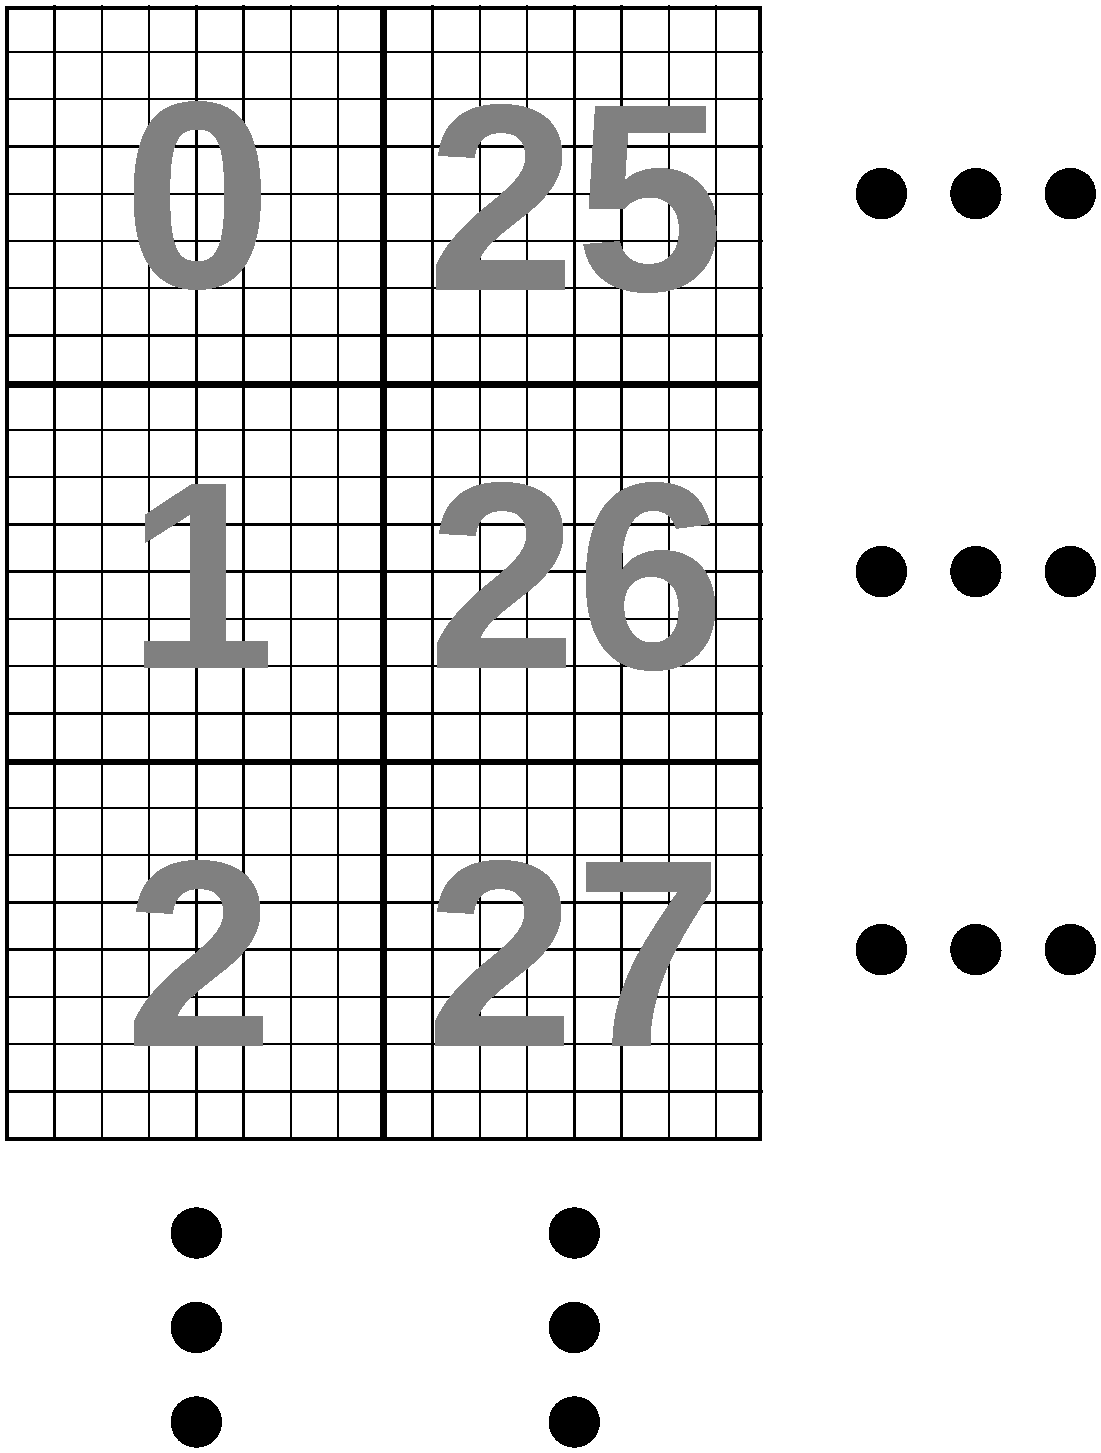
\includegraphics[width=0.7\textwidth]{images/illustrations/char-tile-grid-vertical-numbered}
\end{center}

Door de tekens zo in verticale kolommen te rangschikken, levert een verticale verplaatsing van één pixel telkens een constante toename van 8 bytes op, zoals hieronder wordt weergegeven:

\begin{center}
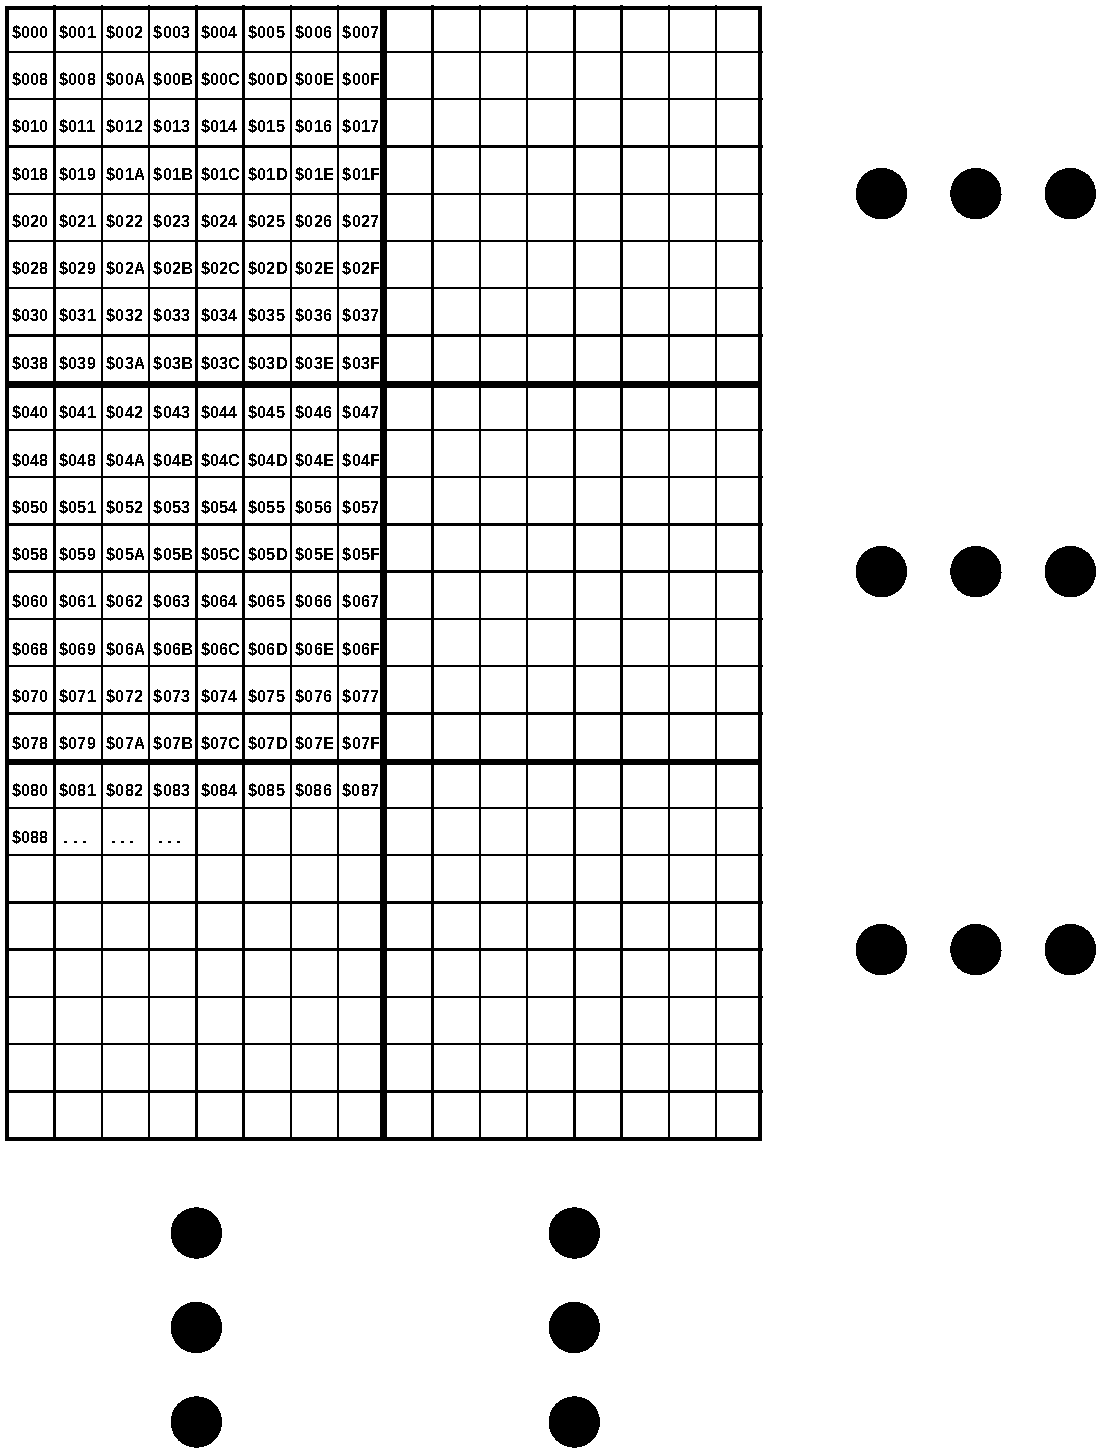
\includegraphics[width=0.7\textwidth]{images/illustrations/char-tile-grid-vertical-addressed}
\end{center}


De skipwaarden voor bron en bestemming maken het ook mogelijk de schaalfactoren in te stellen. Een skipwaarde van \$0100 komt overeen met een verplaatsing van \$01.00 pixel. Wilt u de verticaal gestapelde FCM-indeling gebruiken als doel voor het kopiëren van verticale textuurlijnen, dan moet de bestemmingsskipwaarde \$0800 zijn, d.w.z. 8.0 bytes per pixel. Daarmee wordt een verticale lijn textuurgegevens zonder schaling gekopieerd. Door de bronverplaatsing lager dan \$0100 in te stellen, worden sommige pixels herhaald, waardoor de textuur effectief wordt ingezoomd; stelt u de bronverplaatsing boven \$0100 in, dan worden sommige pixels overgeslagen, waardoor de textuur effectief wordt uitgezoomd. De bestemmingsverplaatsing hoeft gewoonlijk niet te worden aangepast. Let op: de textuurgegevens moeten zo worden opgeslagen dat elke verticale strook aaneengesloten staat, opdat deze modus kan worden gebruikt.

Voor het tekenen van lijnen moet de DMA-controller de schermindeling kennen. Hij moet in het bijzonder weten welk getal moet worden opgeteld bij het adres van de meest rechtse pixel in een kolom FCM-tekens om het adres te berekenen van de pixel die onmiddellijk rechts daarvan verschijnt. Evenzo moet hij weten hoeveel er moet worden opgeteld bij het adres van de onderste pixel in een rij FCM-tekens om het adres te berekenen van de pixel die onmiddellijk onder die pixel verschijnt. Dit biedt flexibele mogelijkheden voor de schermindeling en willekeurige schermafmetingen. U moet daarna ook de helling van de lijn opgeven, of de lijn de X-as of de Y-as als hoofdas heeft en of de helling positief of negatief is.

Het bestand {\tt test\_290.c} in de repository \url{https://github.com/mega65/mega65-tools} bevat een voorbeeld van het gebruik van deze voorzieningen om hardware-versnelde lijntekening te implementeren. Deze aanpak is {\em zeer} snel, want de lijnen worden getekend met de volledige DMA-vulsnelheid, d.w.z. ongeveer 40.5 miljoen pixels per seconde.

\section{Inline-DMA-lijsten}
\index{DMA!Inline-DMA-lijsten}
\index{Inline-DMA-lijsten}

Gewoonlijk moet u een apart geheugengebied inrichten dat de DMA-lijst bevat en vervolgens het adres van dat gebied in de DMA-adresregisters op \$D70x laden. Omdat de DMA-controller van de MEGA65 deel uitmaakt van de CPU, ondersteunt deze bovendien een uiterst handige extra modus: de inline-DMA-lijstmodus.

Deze modus werkt zoals de Enhanced-DMA-modus, met dit verschil dat de DMA-lijst wordt gelezen vanaf de huidige waarde van het Program Counter (PC)-register. Om deze modus te gebruiken, schrijft u een willekeurige waarde naar \$D707. Hiermee start u onmiddellijk een DMA-taak, waarvan de lijst staat in de bytes die direct volgen op de instructie die naar \$D707 schrijft.

De DMA-lijst kan uit één enkele taak bestaan of, zoals bij elke andere DMA-taak, uit meerdere gekoppelde taken. Het echte kunststuk is dat de programmateller wordt gezet op het eerstvolgende adres na het einde van de DMA-lijst en dat de DMA-lijst wordt gelezen uit de huidige geheugenindeling van de CPU. Dit betekent dat u code met DMA-lijsten vanuit elke geheugenbank kunt uitvoeren, zonder dat u hoeft na te gaan in welke bank die code staat.

Het volgende codevoorbeeld wist bijvoorbeeld het scherm in de C65-modus en laat de rand daarna eindeloos flikkeren:

\begin{asmcodesmall}
  STA $D707
  .byte $00   ; end of job options
  .byte $03   ; fill
  .word 2000  ; count
  .word $0020 ; value
  .byte $00   ; src bank
  .word $0800 ; dst
  .byte $00   ; dst bank
  .byte $00   ; cmd hi
  .word $0000 ; modulo / ignored
foo:
  INC $D020
  JMP foo
\end{asmcodesmall}

\section{Audio-DMA}
\index{Digitale audio}
\index{DMA-audio}
\index{Amiga\texttrademark{}-stijl audio}
\index{MOD-stijl audio}
De MEGA65 beschikt over vier kanalen voor DMA-aangestuurde geluidsweergave, die in plaats van de directe digitale audioregisters op \$D6F8-\$D6FB gebruikt kunnen worden. U moet dus kiezen welke van deze twee bronnen u aan de audio-crossbar-mixer wilt toevoeren. Die keuze wordt gemaakt via het AUDEN-signaal (bit 7 van \$D711), dat tegelijkertijd de audio-DMA-functie in de processor inschakelt en de audio-crossbar-mixer opdraagt de audio van deze bron te gebruiken in plaats van de digitale audioregisters op \$D6F8-\$D6FB. Indien u naast de audio-DMA-kanalen geen ander geluid wenst, kan de audio-crossbar-mixer worden omzeild en kan de DMA-audio op vol volume worden afgespeeld door het NOMIX-signaal te zetten (bit 4 van \$D711). De omzeiling geldt alleen voor de PWM-audio-uitgangen (de 3,5mm-audioaansluiting op R3 en oudere borden): op die uitgangen is er geen geluid van de SID's, FM, microfoons of andere bronnen beschikbaar. HDMI-audio, en de audio-DAC op R4 en nieuwere borden, dragen altijd de uitvoer van de audio-crossbar-mixer. Alle overige bits van \$D711 moeten gewoonlijk nul blijven; schrijf dus \$80 naar \$D711 om audio-DMA in te schakelen.

Twee kanalen vormen het linker digitale audiokanaal en de twee andere het rechter digitale audiokanaal. Deze linker- en rechterkanalen worden vervolgens aan de audio-crossbar-mixer van de MEGA65 toegevoerd.

Omdat de DMA-controller deel uitmaakt van de processor van de MEGA65 en de MEGA65 geen gereserveerde busesleuven heeft voor multimedia-bewerkingen, gebruikt de MEGA65 ongebruikte CPU-cycli om DMA op de achtergrond uit te voeren. Hiervoor moet de CPU van de MEGA65 in de modus ``full speed'' staan, d.w.z. op ongeveer 40 MHz. In deze modus treedt bij het lezen van een operand uit het geheugen telkens een wachtcyclus op. Elke instructie die een byte uit het geheugen laadt, creëert daardoor één impliciete audio-DMA-sleuf. In de praktijk is dit zelden een probleem, behalve wanneer de processor in een zeer strakke lus wacht. Om ervoor te zorgen dat de audio op de achtergrond blijft spelen, moeten dergelijke lussen een leesinstructie bevatten, zoals:

\begin{asmcodesmall}
  ; Ensure loop has at least one idle cycle for
  ; audio DMA
loop:
  LDA $1234
  JMP loop
\end{asmcodesmall}

Elk van de vier DMA-kanalen wordt geconfigureerd met een blok van 16 registers op respectievelijk \$D720, \$D730, \$D740 en \$D750. Wij lichten de registers van het eerste kanaal, kanaal 0, toe op \$D720 -- \$D72F.

\subsection{Adresbeheer voor samples}

Om een audiosample af te spelen, moet u eerst het startadres van het sample opgeven. Dit is een 24-bits adres dat in het hoofd-chipgeheugen van de MEGA65 moet liggen. U schrijft het adres daartoe in \$D72A -- \$D72C. Dat is het adres van de eerste samplewaarde die wordt afgespeeld. Vervolgens moet u het eindadres van het sample opgeven in \$D727 -- \$D728. Let echter op: dit is slechts 16 bits. Dat komt doordat de MEGA65 bij de controle of het einde van een sample is bereikt, alleen de onderste 16 bits van het adres vergelijkt. In de praktijk betekent dit dat samples niet groter dan 64 KB kunnen zijn. Bevat het sample een gedeelte dat herhaald moet worden, dan moet het startadres van dat herhalende gedeelte in \$D721 -- \$D723 worden geladen en moet de CH0LOOP-bit worden gezet (bit 6 van \$D720).

U kunt op elk moment het huidige sampleadres bepalen door de registers op \$D72A -- \$D72C te lezen. Let echter op: deze registers worden niet vergrendeld, zodat de waarden tijdens het lezen kunnen worden bijgewerkt, tenzij u het kanaal eerst stopt door het CH0EN-signaal te wissen.

\subsection{Afspeelfrequentie en volume van samples}

De MEGA65 regelt de afspeelsnelheid van audio-DMA-samples met een 24-bits teller. Telkens wanneer de 24-bits teller overloopt, wordt de volgende samplewaarde opgevraagd. De samplesnelheid stelt u in door de waarde te kiezen die elke CPU-cyclus aan deze teller wordt toegevoegd. Een waarde van \$FFFFFF levert derhalve een samplerate van bijna 40.5 MHz op. In de praktijk zijn samplerates boven enkele megahertz echter niet mogelijk, omdat daarvoor onvoldoende ongebruikte CPU-cycli beschikbaar zijn en er anders vervormd geluid ontstaat. Ook onder die grens moet u ervoor zorgen dat de ongebruikte cycli voldoende vaak en voldoende verspreid door de instructiestroom van de processor voorkomen, om vervorming te vermijden. Bij typische samplerates onder 16 kHz en het gebruik van 8-bits samples zijn deze effecten voor normale instructiestromen doorgaans verwaarloosbaar, zodat voor normaal audio-afspelen gewoonlijk geen speciale maatregelen nodig zijn.

Aan de andere kant van de schaal zijn samplefrequenties van slechts 40.5 MHz/$2^{24}$= 2.4 samples per seconde mogelijk. Dat is laag genoeg voor zelfs de meest veeleisende infrageluidstoepassingen.

Het volume wordt geregeld door \$D729 in te stellen. Het maximale volume wordt bereikt met de waarde \$FF, terwijl een waarde van \$00 het kanaal volledig dempt. De eerste twee audiokanalen worden normaal gesproken aan de linkerzijde toegewezen en de tweede twee aan de rechterzijde. De MEGA65 beschikt echter over afzonderlijke volumeregelaars voor de tegenoverliggende kanalen. Om audio-DMA-kanaal 0 bijvoorbeeld op vol volume aan zowel de linker- als de rechterkant van de audio-uitgang af te spelen, stelt u zowel \$D729 als \$D71C in op \$FF. Dit maakt het pannen van de vier audio-DMA-kanalen mogelijk.

Zowel de frequentie als het volume kunnen tijdens het afspelen van een sample vrij worden aangepast om verschillende effecten te verkrijgen.

\subsection{Zuivere sinusgolf}

Wanneer het nodig is een stabiele sinusgolf te produceren, met name bij hogere frequenties, voorziet een speciale modus hierin. Door het CH0SINE-signaal te zetten, speelt het audiokanaal een sinusgolfpatroon van 32 bytes met 16-bits samples af. De sample-adressen moeten nog steeds worden ingesteld, alsof de sinusgolftabel zich in de onderste 64 bytes van het geheugen bevindt; de normale adresgeneratielogica wordt namelijk ook in deze modus gebruikt. In deze modus worden geen audio-DMA-fetches uitgevoerd, zodat alle vervormingsbronnen worden vermeden die het gevolg zijn van de onregelmatige spreiding van inactieve cycli in de instructiestroom van de processor.

Dit kan worden gebruikt om sinusgolven te produceren in zowel het hoorbare bereik als ver daarboven in het ultrasone bereik, bij frequenties die 60000 Hz overschrijden, mits de MEGA65 is aangesloten op een geschikte luidsprekeropstelling.

\subsection{Regeling van het afspelen van samples}

Om een kanaal een sample te laten afspelen, zet u het CH0EN-signaal (\$D720 bit 7). Het sample wordt afgespeeld tot het zijn einde bereikt, tenzij het CH0LOOP-signaal eveneens is gezet. Wanneer een sample klaar is met afspelen, wordt de CH0STP-vlag gezet. Het audio-DMA-subsysteem kan op dit moment geen interrupts genereren.

Anders dan de Amiga\texttrademark{} biedt het audio-DMA-systeem van de MEGA65 ondersteuning voor zowel 8- als 16-bits samples. Het ondersteunt ook samengepakte 4-bits samples, waarbij van elk sample-byte de lagere of de hogere nibble wordt afgespeeld. Hierdoor kunnen twee afzonderlijke samples hetzelfde byte bezetten, waarmee de benodigde opslagruimte voor twee samples van gelijke lengte effectief wordt gehalveerd.

\section{F018 ``DMAgic'' DMA-controller}

\setlength{\tabcolsep}{0pt}
\begin{longtable}{|C{12.5mm}|C{12.5mm}|C{12.5mm}|C{12.5mm}|C{12.5mm}|C{12.5mm}|C{12.5mm}|C{12.5mm}|C{12.5mm}|C{12.5mm}|}
\hline
{\bf{HEX}} & {\bf{DEC}} & {\bf{DB7}} & {\bf{DB6}} & {\bf{DB5}} & {\bf{DB4}} & {\bf{DB3}} & {\bf{DB2}} & {\bf{DB1}} & {\bf{DB0}} \\
\hline
\endfirsthead
\multicolumn{3}{l@{}}{\ldots vervolgd}\\
\hline
{\bf{HEX}} & {\bf{DEC}} & {\bf{DB7}} & {\bf{DB6}} & {\bf{DB5}} & {\bf{DB4}} & {\bf{DB3}} & {\bf{DB2}} & {\bf{DB1}} & {\bf{DB0}} \\
\endhead
\multicolumn{3}{l@{}}{vervolgd \ldots}\\
\endfoot
\hline
\endlastfoot
\footnotesize  D700\index{Registers!\$D700} \index{Registers!55040} & \footnotesize 55040 & \multicolumn{8}{c|}{\footnotesize ADDRLSBTRIG\index{Registers!ADDRLSBTRIG}}\\
\hline
\footnotesize  D701\index{Registers!\$D701} \index{Registers!55041} & \footnotesize 55041 & \multicolumn{8}{c|}{\footnotesize ADDRMSB\index{Registers!ADDRMSB}}\\
\hline
\footnotesize  D702\index{Registers!\$D702} \index{Registers!55042} & \footnotesize 55042 & \footnotesize WITHIO & \multicolumn{7}{c|}{\footnotesize ADDRBANK\index{Registers!ADDRBANK}}\\
\hline
\end{longtable}
\begin{itemize}
\item{\bf{ADDRBANK}\index{Registers!ADDRBANK}} Adresbank van de DMA-lijst (bits 16 - 22). Schrijven wist \$D704.
\item{\bf{ADDRLSBTRIG}\index{Registers!ADDRLSBTRIG}} DMAgic-LSB van het adres van de DMA-lijst (bits 0 - 7); start DMA wanneer erin wordt geschreven
\item{\bf{ADDRMSB}\index{Registers!ADDRMSB}} Hoge byte van het adres van de DMA-lijst (bits 8 - 15)
\item{\bf{WITHIO}\index{Registers!WITHIO}} DMA-withio-vlag (onbenut)
\end{itemize}


\section{Uitbreidingen van de MEGA65-DMA-controller}

\setlength{\tabcolsep}{0pt}
\begin{longtable}{|C{12.5mm}|C{12.5mm}|C{12.5mm}|C{12.5mm}|C{12.5mm}|C{12.5mm}|C{12.5mm}|C{12.5mm}|C{12.5mm}|C{12.5mm}|}
\hline
{\bf{HEX}} & {\bf{DEC}} & {\bf{DB7}} & {\bf{DB6}} & {\bf{DB5}} & {\bf{DB4}} & {\bf{DB3}} & {\bf{DB2}} & {\bf{DB1}} & {\bf{DB0}} \\
\hline
\endfirsthead
\multicolumn{3}{l@{}}{\ldots vervolgd}\\
\hline
{\bf{HEX}} & {\bf{DEC}} & {\bf{DB7}} & {\bf{DB6}} & {\bf{DB5}} & {\bf{DB4}} & {\bf{DB3}} & {\bf{DB2}} & {\bf{DB1}} & {\bf{DB0}} \\
\endhead
\multicolumn{3}{l@{}}{vervolgd \ldots}\\
\endfoot
\hline
\endlastfoot
\footnotesize  D703\index{Registers!\$D703} \index{Registers!55043} & \footnotesize 55043 & \multicolumn{6}{c|}{\footnotesize --}& \footnotesize NOMBWRAP & \footnotesize EN018B \\
\hline
\footnotesize  D704\index{Registers!\$D704} \index{Registers!55044} & \footnotesize 55044 & \multicolumn{8}{c|}{\footnotesize ADDRMB\index{Registers!ADDRMB}}\\
\hline
\footnotesize  D705\index{Registers!\$D705} \index{Registers!55045} & \footnotesize 55045 & \multicolumn{8}{c|}{\footnotesize ETRIG\index{Registers!ETRIG}}\\
\hline
\footnotesize  D706\index{Registers!\$D706} \index{Registers!55046} & \footnotesize 55046 & \multicolumn{8}{c|}{\footnotesize ETRIGMAPD\index{Registers!ETRIGMAPD}}\\
\hline
\footnotesize  D707\index{Registers!\$D707} \index{Registers!55047} & \footnotesize 55047 & \multicolumn{8}{c|}{\footnotesize ETRIGINLINE\index{Registers!ETRIGINLINE}}\\
\hline
\footnotesize  D70E\index{Registers!\$D70E} \index{Registers!55054} & \footnotesize 55054 & \multicolumn{8}{c|}{\footnotesize ADDRLSB\index{Registers!ADDRLSB}}\\
\hline
\footnotesize  D711\index{Registers!\$D711} \index{Registers!55057} & \footnotesize 55057 & \footnotesize AUDEN & \footnotesize BLKD & \footnotesize AUD\-WRBLK & \footnotesize NOMIX & \footnotesize -- & \multicolumn{3}{c|}{\footnotesize AUD\-BLKTO\index{Registers!AUDBLKTO}}\\
\hline
\footnotesize  D712\index{Registers!\$D712} \index{Registers!55058} & \footnotesize 55058 & \footnotesize DBG\-LFTCLP & \footnotesize DBG\-RGTCLP & \multicolumn{4}{c|}{\footnotesize --}& \footnotesize CHANSWAP & \footnotesize -- \\
\hline
\footnotesize  D713\index{Registers!\$D713} \index{Registers!55059} & \footnotesize 55059 & \footnotesize IRQ\-CH0FLG & \footnotesize IRQ\-CH1FLG & \footnotesize IRQ\-CH2FLG & \footnotesize IRQ\-CH3FLG & \footnotesize IRQ\-CH0ENA & \footnotesize IRQ\-CH1ENA & \footnotesize IRQ\-CH2ENA & \footnotesize IRQ\-CH3ENA \\
\hline
\footnotesize  D714\index{Registers!\$D714} \index{Registers!55060} & \footnotesize 55060 & \multicolumn{8}{c|}{\footnotesize IRQ\-CH0OFFS\index{Registers!CHXOFFS}}\\
\hline
\footnotesize  D715\index{Registers!\$D715} \index{Registers!55061} & \footnotesize 55061 & \multicolumn{8}{c|}{\footnotesize IRQ\-CH1OFFS\index{Registers!IRQCH1OFFS}}\\
\hline
\footnotesize  D716\index{Registers!\$D716} \index{Registers!55062} & \footnotesize 55062 & \multicolumn{8}{c|}{\footnotesize IRQ\-CH2OFFS\index{Registers!IRQCH2OFFS}}\\
\hline
\footnotesize  D717\index{Registers!\$D717} \index{Registers!55063} & \footnotesize 55063 & \multicolumn{8}{c|}{\footnotesize IRQ\-CH3OFFS\index{Registers!IRQCH3OFFS}}\\
\hline
\footnotesize  D71C\index{Registers!\$D71C} \index{Registers!55068} & \footnotesize 55068 & \multicolumn{8}{c|}{\footnotesize CH0RVOL\index{Registers!CH0RVOL}}\\
\hline
\footnotesize  D71D\index{Registers!\$D71D} \index{Registers!55069} & \footnotesize 55069 & \multicolumn{8}{c|}{\footnotesize CH1RVOL\index{Registers!CH1RVOL}}\\
\hline
\footnotesize  D71E\index{Registers!\$D71E} \index{Registers!55070} & \footnotesize 55070 & \multicolumn{8}{c|}{\footnotesize CH2LVOL\index{Registers!CH2LVOL}}\\
\hline
\footnotesize  D71F\index{Registers!\$D71F} \index{Registers!55071} & \footnotesize 55071 & \multicolumn{8}{c|}{\footnotesize CH3LVOL\index{Registers!CH3LVOL}}\\
\hline
\footnotesize  D720\index{Registers!\$D720} \index{Registers!55072} & \footnotesize 55072 & \footnotesize CH0\-EN & \footnotesize CH0\-LOOP & \footnotesize CH0\-SGN & \footnotesize CH0\-SINE & \footnotesize CH0\-STP & \footnotesize -- & \multicolumn{2}{c|}{\footnotesize CH0\-SBITS\index{Registers!CHXSBITS}}\\
\hline
\footnotesize  D721\index{Registers!\$D721} \index{Registers!55073} & \footnotesize 55073 & \multicolumn{8}{c|}{\footnotesize CH0BADDRLSB\index{Registers!CHXBADDRLSB}}\\
\hline
\footnotesize  D722\index{Registers!\$D722} \index{Registers!55074} & \footnotesize 55074 & \multicolumn{8}{c|}{\footnotesize CH0BADDRMSB\index{Registers!CHXBADDRMSB}}\\
\hline
\footnotesize  D723\index{Registers!\$D723} \index{Registers!55075} & \footnotesize 55075 & \multicolumn{8}{c|}{\footnotesize CH0BADDRBNK\index{Registers!CHXBADDRBNK}}\\
\hline
\footnotesize  D724\index{Registers!\$D724} \index{Registers!55076} & \footnotesize 55076 & \multicolumn{8}{c|}{\footnotesize CH0FREQ0\index{Registers!CHXFREQ0}}\\
\hline
\footnotesize  D725\index{Registers!\$D725} \index{Registers!55077} & \footnotesize 55077 & \multicolumn{8}{c|}{\footnotesize CH0FREQ1\index{Registers!CHXFREQ1}}\\
\hline
\footnotesize  D726\index{Registers!\$D726} \index{Registers!55078} & \footnotesize 55078 & \multicolumn{8}{c|}{\footnotesize CH0FREQ2\index{Registers!CHXFREQ2}}\\
\hline
\footnotesize  D727\index{Registers!\$D727} \index{Registers!55079} & \footnotesize 55079 & \multicolumn{8}{c|}{\footnotesize CH0TADDRLSB\index{Registers!CHXTADDRL}}\\
\hline
\footnotesize  D728\index{Registers!\$D728} \index{Registers!55080} & \footnotesize 55080 & \multicolumn{8}{c|}{\footnotesize CH0TADDRMSB\index{Registers!CHXTADDRM}}\\
\hline
\footnotesize  D729\index{Registers!\$D729} \index{Registers!55081} & \footnotesize 55081 & \multicolumn{8}{c|}{\footnotesize CH0VOLUME\index{Registers!CHXVOLUME}}\\
\hline
\footnotesize  D72A\index{Registers!\$D72A} \index{Registers!55082} & \footnotesize 55082 & \multicolumn{8}{c|}{\footnotesize CH0CURADDRLSB\index{Registers!CHXCURADDRLSB}}\\
\hline
\footnotesize  D72B\index{Registers!\$D72B} \index{Registers!55083} & \footnotesize 55083 & \multicolumn{8}{c|}{\footnotesize CH0CURADDRMSB\index{Registers!CHXCURADDRMSB}}\\
\hline
\footnotesize  D72C\index{Registers!\$D72C} \index{Registers!55084} & \footnotesize 55084 & \multicolumn{8}{c|}{\footnotesize CH0CURADDRBNK\index{Registers!CHXCURADDRBNK}}\\
\hline
\footnotesize  D72D\index{Registers!\$D72D} \index{Registers!55085} & \footnotesize 55085 & \multicolumn{8}{c|}{\footnotesize CH0TMGCNT0\index{Registers!CHXTMGCNT0}}\\
\hline
\footnotesize  D72E\index{Registers!\$D72E} \index{Registers!55086} & \footnotesize 55086 & \multicolumn{8}{c|}{\footnotesize CH0TMGCNT1\index{Registers!CHXTMGCNT1}}\\
\hline
\footnotesize  D72F\index{Registers!\$D72F} \index{Registers!55087} & \footnotesize 55087 & \multicolumn{8}{c|}{\footnotesize CH0TMGCNT2\index{Registers!CHXTMGCNT2}}\\
\hline
\footnotesize  D730\index{Registers!\$D730} \index{Registers!55088} & \footnotesize 55088 & \footnotesize CH1\-EN & \footnotesize CH1\-LOOP & \footnotesize CH1\-SGN & \footnotesize CH1\-SINE & \footnotesize CH1\-STP & \footnotesize -- & \multicolumn{2}{c|}{\footnotesize CH1\-SBITS\index{Registers!CH1SBITS}}\\
\hline
\footnotesize  D731\index{Registers!\$D731} \index{Registers!55089} & \footnotesize 55089 & \multicolumn{8}{c|}{\footnotesize CH1BADDRLSB\index{Registers!CH1BADDRLSB}}\\
\hline
\footnotesize  D732\index{Registers!\$D732} \index{Registers!55090} & \footnotesize 55090 & \multicolumn{8}{c|}{\footnotesize CH1BADDRMSB\index{Registers!CH1BADDRMSB}}\\
\hline
\footnotesize  D733\index{Registers!\$D733} \index{Registers!55091} & \footnotesize 55091 & \multicolumn{8}{c|}{\footnotesize CH1BADDRBNK\index{Registers!CH1BADDRBNK}}\\
\hline
\footnotesize  D734\index{Registers!\$D734} \index{Registers!55092} & \footnotesize 55092 & \multicolumn{8}{c|}{\footnotesize CH1FREQ0\index{Registers!CH1FREQ0}}\\
\hline
\footnotesize  D735\index{Registers!\$D735} \index{Registers!55093} & \footnotesize 55093 & \multicolumn{8}{c|}{\footnotesize CH1FREQ1\index{Registers!CH1FREQ1}}\\
\hline
\footnotesize  D736\index{Registers!\$D736} \index{Registers!55094} & \footnotesize 55094 & \multicolumn{8}{c|}{\footnotesize CH1FREQ2\index{Registers!CH1FREQ2}}\\
\hline
\footnotesize  D737\index{Registers!\$D737} \index{Registers!55095} & \footnotesize 55095 & \multicolumn{8}{c|}{\footnotesize CH1TADDRLSB\index{Registers!CH1TADDRLSB}}\\
\hline
\footnotesize  D738\index{Registers!\$D738} \index{Registers!55096} & \footnotesize 55096 & \multicolumn{8}{c|}{\footnotesize CH1TADDRMSB\index{Registers!CH1TADDRMSB}}\\
\hline
\footnotesize  D739\index{Registers!\$D739} \index{Registers!55097} & \footnotesize 55097 & \multicolumn{8}{c|}{\footnotesize CH1VOLUME\index{Registers!CH1VOLUME}}\\
\hline
\footnotesize  D73A\index{Registers!\$D73A} \index{Registers!55098} & \footnotesize 55098 & \multicolumn{8}{c|}{\footnotesize CH1CURADDRLSB\index{Registers!CH1CURADDRLSB}}\\
\hline
\footnotesize  D73B\index{Registers!\$D73B} \index{Registers!55099} & \footnotesize 55099 & \multicolumn{8}{c|}{\footnotesize CH1CURADDRMSB\index{Registers!CH1CURADDRMSB}}\\
\hline
\footnotesize  D73C\index{Registers!\$D73C} \index{Registers!55100} & \footnotesize 55100 & \multicolumn{8}{c|}{\footnotesize CH1CURADDRBNK\index{Registers!CH1CURADDRBNK}}\\
\hline
\footnotesize  D73D\index{Registers!\$D73D} \index{Registers!55101} & \footnotesize 55101 & \multicolumn{8}{c|}{\footnotesize CH1TMGCNT0\index{Registers!CH1TMGCNT0}}\\
\hline
\footnotesize  D73E\index{Registers!\$D73E} \index{Registers!55102} & \footnotesize 55102 & \multicolumn{8}{c|}{\footnotesize CH1TMGCNT1\index{Registers!CH1TMGCNT1}}\\
\hline
\footnotesize  D73F\index{Registers!\$D73F} \index{Registers!55103} & \footnotesize 55103 & \multicolumn{8}{c|}{\footnotesize CH1TMGCNT2\index{Registers!CH1TMGCNT2}}\\
\hline
\footnotesize  D740\index{Registers!\$D740} \index{Registers!55104} & \footnotesize 55104 & \footnotesize CH2\-EN & \footnotesize CH2\-LOOP & \footnotesize CH2\-SGN & \footnotesize CH2\-SINE & \footnotesize CH2\-STP & \footnotesize -- & \multicolumn{2}{c|}{\footnotesize CH2\-SBITS\index{Registers!CH2SBITS}}\\
\hline
\footnotesize  D741\index{Registers!\$D741} \index{Registers!55105} & \footnotesize 55105 & \multicolumn{8}{c|}{\footnotesize CH2BADDRLSB\index{Registers!CH2BADDRLSB}}\\
\hline
\footnotesize  D742\index{Registers!\$D742} \index{Registers!55106} & \footnotesize 55106 & \multicolumn{8}{c|}{\footnotesize CH2BADDRMSB\index{Registers!CH2BADDRMSB}}\\
\hline
\footnotesize  D743\index{Registers!\$D743} \index{Registers!55107} & \footnotesize 55107 & \multicolumn{8}{c|}{\footnotesize CH2BADDRBNK\index{Registers!CH2BADDRBNK}}\\
\hline
\footnotesize  D744\index{Registers!\$D744} \index{Registers!55108} & \footnotesize 55108 & \multicolumn{8}{c|}{\footnotesize CH2FREQ0\index{Registers!CH2FREQ0}}\\
\hline
\footnotesize  D745\index{Registers!\$D745} \index{Registers!55109} & \footnotesize 55109 & \multicolumn{8}{c|}{\footnotesize CH2FREQ1\index{Registers!CH2FREQ1}}\\
\hline
\footnotesize  D746\index{Registers!\$D746} \index{Registers!55110} & \footnotesize 55110 & \multicolumn{8}{c|}{\footnotesize CH2FREQ2\index{Registers!CH2FREQ2}}\\
\hline
\footnotesize  D747\index{Registers!\$D747} \index{Registers!55111} & \footnotesize 55111 & \multicolumn{8}{c|}{\footnotesize CH2TADDRLSB\index{Registers!CH2TADDRLSB}}\\
\hline
\footnotesize  D748\index{Registers!\$D748} \index{Registers!55112} & \footnotesize 55112 & \multicolumn{8}{c|}{\footnotesize CH2TADDRMSB\index{Registers!CH2TADDRMSB}}\\
\hline
\footnotesize  D749\index{Registers!\$D749} \index{Registers!55113} & \footnotesize 55113 & \multicolumn{8}{c|}{\footnotesize CH2VOLUME\index{Registers!CH2VOLUME}}\\
\hline
\footnotesize  D74A\index{Registers!\$D74A} \index{Registers!55114} & \footnotesize 55114 & \multicolumn{8}{c|}{\footnotesize CH2CURADDRLSB\index{Registers!CH2CURADDRLSB}}\\
\hline
\footnotesize  D74B\index{Registers!\$D74B} \index{Registers!55115} & \footnotesize 55115 & \multicolumn{8}{c|}{\footnotesize CH2CURADDRMSB\index{Registers!CH2CURADDRMSB}}\\
\hline
\footnotesize  D74C\index{Registers!\$D74C} \index{Registers!55116} & \footnotesize 55116 & \multicolumn{8}{c|}{\footnotesize CH2CURADDRBNK\index{Registers!CH2CURADDRBNK}}\\
\hline
\footnotesize  D74D\index{Registers!\$D74D} \index{Registers!55117} & \footnotesize 55117 & \multicolumn{8}{c|}{\footnotesize CH2TMGCNT0\index{Registers!CH2TMGCNT0}}\\
\hline
\footnotesize  D74E\index{Registers!\$D74E} \index{Registers!55118} & \footnotesize 55118 & \multicolumn{8}{c|}{\footnotesize CH2TMGCNT1\index{Registers!CH2TMGCNT1}}\\
\hline
\footnotesize  D74F\index{Registers!\$D74F} \index{Registers!55119} & \footnotesize 55119 & \multicolumn{8}{c|}{\footnotesize CH2TMGCNT2\index{Registers!CH2TMGCNT2}}\\
\hline
\footnotesize  D750\index{Registers!\$D750} \index{Registers!55120} & \footnotesize 55120 & \footnotesize CH3\-EN & \footnotesize CH3\-LOOP & \footnotesize CH3\-SGN & \footnotesize CH3\-SINE & \footnotesize CH3\-STP & \footnotesize -- & \multicolumn{2}{c|}{\footnotesize CH3\-SBITS\index{Registers!CH3SBITS}}\\
\hline
\footnotesize  D751\index{Registers!\$D751} \index{Registers!55121} & \footnotesize 55121 & \multicolumn{8}{c|}{\footnotesize CH3BADDRLSB\index{Registers!CH3BADDRLSB}}\\
\hline
\footnotesize  D752\index{Registers!\$D752} \index{Registers!55122} & \footnotesize 55122 & \multicolumn{8}{c|}{\footnotesize CH3BADDRMSB\index{Registers!CH3BADDRMSB}}\\
\hline
\footnotesize  D753\index{Registers!\$D753} \index{Registers!55123} & \footnotesize 55123 & \multicolumn{8}{c|}{\footnotesize CH3BADDRBNK\index{Registers!CH3BADDRBNK}}\\
\hline
\footnotesize  D754\index{Registers!\$D754} \index{Registers!55124} & \footnotesize 55124 & \multicolumn{8}{c|}{\footnotesize CH3FREQ0\index{Registers!CH3FREQ0}}\\
\hline
\footnotesize  D755\index{Registers!\$D755} \index{Registers!55125} & \footnotesize 55125 & \multicolumn{8}{c|}{\footnotesize CH3FREQ1\index{Registers!CH3FREQ1}}\\
\hline
\footnotesize  D756\index{Registers!\$D756} \index{Registers!55126} & \footnotesize 55126 & \multicolumn{8}{c|}{\footnotesize CH3FREQ2\index{Registers!CH3FREQ2}}\\
\hline
\footnotesize  D757\index{Registers!\$D757} \index{Registers!55127} & \footnotesize 55127 & \multicolumn{8}{c|}{\footnotesize CH3TADDRLSB\index{Registers!CH3TADDRLSB}}\\
\hline
\footnotesize  D758\index{Registers!\$D758} \index{Registers!55128} & \footnotesize 55128 & \multicolumn{8}{c|}{\footnotesize CH3TADDRMSB\index{Registers!CH3TADDRMSB}}\\
\hline
\footnotesize  D759\index{Registers!\$D759} \index{Registers!55129} & \footnotesize 55129 & \multicolumn{8}{c|}{\footnotesize CH3VOLUME\index{Registers!CH3VOLUME}}\\
\hline
\footnotesize  D75A\index{Registers!\$D75A} \index{Registers!55130} & \footnotesize 55130 & \multicolumn{8}{c|}{\footnotesize CH3CURADDRLSB\index{Registers!CH3CURADDRLSB}}\\
\hline
\footnotesize  D75B\index{Registers!\$D75B} \index{Registers!55131} & \footnotesize 55131 & \multicolumn{8}{c|}{\footnotesize CH3CURADDRMSB\index{Registers!CH3CURADDRMSB}}\\
\hline
\footnotesize  D75C\index{Registers!\$D75C} \index{Registers!55132} & \footnotesize 55132 & \multicolumn{8}{c|}{\footnotesize CH3CURADDRBNK\index{Registers!CH3CURADDRBNK}}\\
\hline
\footnotesize  D75D\index{Registers!\$D75D} \index{Registers!55133} & \footnotesize 55133 & \multicolumn{8}{c|}{\footnotesize CH3TMGCNT0\index{Registers!CH3TMGCNT0}}\\
\hline
\footnotesize  D75E\index{Registers!\$D75E} \index{Registers!55134} & \footnotesize 55134 & \multicolumn{8}{c|}{\footnotesize CH3TMGCNT1\index{Registers!CH3TMGCNT1}}\\
\hline
\footnotesize  D75F\index{Registers!\$D75F} \index{Registers!55135} & \footnotesize 55135 & \multicolumn{8}{c|}{\footnotesize CH3TMGCNT2\index{Registers!CH3TMGCNT2}}\\
\hline
\end{longtable}
\begin{itemize}
\item{\bf{ADDRLSB}\index{Registers!ADDRLSB}} Lage byte van het DMA-lijstadres (bits 0 - 7) ZONDER EEN DMA-TAAK TE STARTEN (door de Hypervisor gebruikt om taken die DMA gebruiken te ontdooien)
\item{\bf{ADDRMB}\index{Registers!ADDRMB}} Mega-byte van het adres van de DMA-lijst (bits 20 - 27). Overlapt met ADDRBANK!
\item{\bf{AUDBLKTO}\index{Registers!AUDBLKTO}} Time-out van het audio-DMA-blok (alleen-lezen) DEBUG
\item{\bf{AUDEN}\index{Registers!AUDEN}} Schakelt audio-DMA in
\item{\bf{AUDWRBLK}\index{Registers!AUDWRBLK}} Audio-DMA-blokschrijfbewerkingen (samples worden nog steeds gelezen)
\item{\bf{BLKD}\index{Registers!BLKD}} Audio-DMA geblokkeerd (alleen-lezen) DEBUG
\item{\bf{CH0RVOL}\index{Registers!CH0RVOL}} Volume van het rechterkanaal van audio-DMA-kanaal 0
\item{\bf{CH1RVOL}\index{Registers!CH1RVOL}} Volume van het rechterkanaal van audio-DMA-kanaal 1
\item{\bf{CH2LVOL}\index{Registers!CH2LVOL}} Volume van het linkerkanaal van audio-DMA-kanaal 2
\item{\bf{CH3LVOL}\index{Registers!CH3LVOL}} Volume van het linkerkanaal van audio-DMA-kanaal 3
\item{\bf{CHANSWAP}\index{Registers!CHANSWAP}} Omwisseling van de audio-DMA-kanalen
\item{\bf{CHXBADDRBNK}\index{Registers!CHXBADDRBNK}} Basisadres van audio-DMA-kanaal X (bits 16 - 23)
\item{\bf{CHXBADDRLSB}\index{Registers!CHXBADDRLSB}} Basisadres van audio-DMA-kanaal X (bits 0 - 7)
\item{\bf{CHXBADDRMSB}\index{Registers!CHXBADDRMSB}} Basisadres van audio-DMA-kanaal X (bits 8 - 15)
\item{\bf{CHXCURADDRBNK}\index{Registers!CHXCURADDRBNK}} Huidig adres van audio-DMA-kanaal X (bits 16 - 23)
\item{\bf{CHXCURADDRLSB}\index{Registers!CHXCURADDRLSB}} Huidig adres van audio-DMA-kanaal X (bits 0 - 7)
\item{\bf{CHXCURADDRMSB}\index{Registers!CHXCURADDRMSB}} Huidig adres van audio-DMA-kanaal X (bits 8 - 15)
\item{\bf{CHXEN}\index{Registers!CHXEN}} Schakelt audio-DMA-kanaal X in
\item{\bf{CHXENA}\index{Registers!CHXENA}} Audio-DMA-IRQ van kanaal X ingeschakeld
\item{\bf{CHXFLG}\index{Registers!CHXFLG}} Vlag die wordt gezet wanneer een gebeurtenis de audio-DMA-IRQ van kanaal X activeert
\item{\bf{CHXFREQ0}\index{Registers!CHXFREQ0}} Frequentie van audio-DMA-kanaal X (bits 0 - 7)
\item{\bf{CHXFREQ1}\index{Registers!CHXFREQ1}} Frequentie van audio-DMA-kanaal X (bits 8 - 15)
\item{\bf{CHXFREQ2}\index{Registers!CHXFREQ2}} Frequentie van audio-DMA-kanaal X (bits 16 - 23)
\item{\bf{CHXLOOP}\index{Registers!CHXLOOP}} Schakelt looping van audio-DMA-kanaal X in
\item{\bf{CHXOFFS}\index{Registers!CHXOFFS}} IRQ-adresoffset van audio-DMA-kanaal X (bits 15 - 8)
\item{\bf{CHXSBITS}\index{Registers!CHXSBITS}} Sample-bits van audio-DMA-kanaal X (11=16, 10=8, 01=hogere nibble, 00=lagere nibble)
\item{\bf{CHXSINE}\index{Registers!CHXSINE}} Audio-DMA-kanaal X speelt een sinusgolf van 32 samples af in plaats van DMA-gegevens
\item{\bf{CHXSTP}\index{Registers!CHXSTP}} Stopvlag van audio-DMA-kanaal X
\item{\bf{CHXTADDRL}\index{Registers!CHXTADDRL}} Topadres van audio-DMA-kanaal X (bits 0 - 7)
\item{\bf{CHXTADDRM}\index{Registers!CHXTADDRM}} Topadres van audio-DMA-kanaal X (bits 8 - 15)
\item{\bf{CHXTMGCNT0}\index{Registers!CHXTMGCNT0}} Timingteller van audio-DMA-kanaal X (bits 0 - 7)
\item{\bf{CHXTMGCNT1}\index{Registers!CHXTMGCNT1}} Timingteller van audio-DMA-kanaal X (bits 8 - 15)
\item{\bf{CHXTMGCNT2}\index{Registers!CHXTMGCNT2}} Timingteller van audio-DMA-kanaal X (bits 16 - 23)
\item{\bf{CHXUSGN}\index{Registers!CHXUSGN}} Sample-teken van audio-DMA-kanaal X: 0=met teken, 1=zonder teken
\item{\bf{CHXVOLUME}\index{Registers!CHXVOLUME}} Afspeelvolume van audio-DMA-kanaal X
\item{\bf{DBGLFTCLP}\index{Registers!DBGLFTCLP}} Audio-DMA links geklipt (alleen-lezen)
\item{\bf{DBGRGTCLP}\index{Registers!DBGRGTCLP}} Audio-DMA rechts geklipt (alleen-lezen)
\item{\bf{EN018B}\index{Registers!EN018B}} Schakelt de F018B-modus van de DMA in (voegt een subcommandobyte toe)
\item{\bf{ETRIG}\index{Registers!ETRIG}} Stel de lage byte van het DMA-lijstadres in (bits 0 - 7) en start de Enhanced DMA-taak met het lijstadres gespecificeerd als 28-bits flat adres (gebruikt de DMA-optielijst)
\item{\bf{ETRIGINLINE}\index{Registers!ETRIGINLINE}} Start de Enhanced DMAgic-taak inline (d.w.z. beginnend bij de PC-waarde, waarbij de PC na afloop aan het einde van de taak wordt gezet)
\item{\bf{ETRIGMAPD}\index{Registers!ETRIGMAPD}} Stel de lage byte van het DMA-lijstadres in (bits 0 - 7) en start de Enhanced DMA-taak met de lijst in de huidige CPU-geheugenindeling (gebruikt de DMA-optielijst)
\item{\bf{NOMBWRAP}\index{Registers!NOMBWRAP}} Schakelt de wrap-around van het bron- en doeladres op de MB-grenzen uit (wordt genegeerd in de Hypervisor-modus)
\item{\bf{NOMIX}\index{Registers!NOMIX}} Audio-DMA omzeilt de audiomixer
\end{itemize}


\section{Niet-geïmplementeerde functionaliteit}

De DMAgic van de MEGA65 ondersteunt op dit moment noch memory-swap- noch mini-term-bewerkingen.

Mini-terms waren bedoeld voor het blitten van bitplanes, hetgeen voor de MEGA65 niet nodig is, aangezien deze veel geavanceerdere tekstmodi en trapsgewijze en fractionele DMA-adresverhoging biedt, waarmee teksturen efficiënt kunnen worden gekopieerd en geschaald. Er is bovendien geen bekende software die ooit van deze voorziening gebruik heeft gemaakt, en het blijft onzeker of deze ooit in enige revisie van de DMAgic-chip in de C65-prototypen is geïmplementeerd.

De memory-swap-bewerking zal naar verwachting worden geïmplementeerd, maar kan in de tussentijd worden omzeild door het eerste gebied naar een derde gebied te kopiëren dat als tijdelijk buffer fungeert, vervolgens het tweede gebied naar het eerste, en het derde naar het tweede.

  \chapter{VIC-IV Video Interface Controller}
\label{cha:viciv}

\section{Kenmerken}De VIC-IV is een vierde generatie Video Interface Controller die speciaal voor de MEGA65 is ontwikkeld en beschikt over een zeer goede backwards compatibility met de VIC-II die in de C64 werd gebruikt en de VIC-III die in de C65 werd gebruikt. De VIC-IV kan geprogrammeerd worden alsof het een van deze voorgangersystemen betreft. Daarnaast ondersteunt het een aantal nieuwe functies. Het is eenvoudig om oudere VIC-II/III-functies te combineren met de nieuwe VIC-IV-functies, waardoor de overstap van de VIC-II of VIC-III naar de VIC-IV net zo eenvoudig is als de overstap van de VIC-II naar de VIC-III destijds. Enkele van de nieuwe functies en verbeteringen van de VIC-IV zijn:

\begin{itemize}
\item {\bf Directe toegang tot 384KB RAM} (ten opzichte van 16KB/64KB met de VIC-II en 128KB met de VIC-III).\item Ondersteuning voor {\bf 32KB 8-bits kleuren-/attribuutgeheugen} (ten opzichte van 2KB op de VIC-III), om zeer grote schermen te ondersteunen.\item {\bf HDTV 720$\times$576 / 800$\times$600 native resolutie} bij zowel 50 Hz als 60 Hz voor {\bf PAL en NTSC}, met {\bf VGA en digitale video}uitvoer.\item {\bf 81 MHz pixelklok} (ten opzichte van $\sim$ 8 MHz met de VIC-II/III), waardoor een breed scala aan nieuwe functies mogelijk wordt.\item Nieuwe 16-kleuren (16$\times$8 pixels per tekencel) en 256-kleuren (8$\times$8 pixels per tekencel) {\bf volkleur-tekstmodi}.\item Ondersteuning voor maximaal {\bf 8.192 unieke tekens in een tekenset}.\item {\bf Vier 256-kleuren paletbanken} (ten opzichte van de enkele paletbank van de VIC-III), die elk een {\bf 23-bits kleurdiepte} ondersteunen (ten opzichte van de 12-bits kleurdiepte van de VIC-III) en die snel kunnen worden gewisseld om nog kleurrijkere afbeeldingen te produceren dan mogelijk is met de VIC-III.\item Scherm-, bitmap-, kleur- en tekengegevens kunnen op elk {\bf adres met byte-nauwkeurigheid} worden gepositioneerd (in tegenstelling tot de vaste 1KB -- 16KB-grenzen van de VIC-II/III).\item {\bf Virtuele schermafmetingen}, die gecombineerd met byte-nauwkeurige gegevensposities {\bf hardware-ondersteuning voor scrollen en pannen in zowel X- als Y-richting} bieden.\item {\bf Nieuwe sprite-modi}: bitplanewijziging, {\bf volkleuren} (15 voorgrondkleuren + transparantie) en getegelde modi, die een breed scala aan nieuwe en spannende sprite-gebaseerde effecten mogelijk maken.\item De mogelijkheid om sprites stapelvormig in bitplane-vorm te rangschikken om {\bf sprites met maximaal 256 kleuren} te produceren.\item Sprites kunnen 64 bits gegevens per rasterlijn gebruiken, waardoor {\bf sprites 64 pixels breed} kunnen zijn bij gebruik van de VIC-II/III mono-/multicolour-modus, of 16 pixels breed bij gebruik van de nieuwe VIC-IV volkleur-spritemodus.\item {\bf Sprite-tegelmodus}, waarmee een sprite horizontaal kan worden herhaald over de volledige rasterlijn, waardoor sprites kunnen worden gebruikt om geanimeerde achtergronden te creëren op een geheugenefficiënte manier.\item Sprites kunnen worden geconfigureerd om een {\bf apart 256-kleurenpalet} te gebruiken in plaats van het palet dat voor andere tekst en afbeeldingen wordt gebruikt, waardoor een kleurrijker beeld mogelijk is.\item {\bf Super-uitgebreide attribuutmodus} die per tekenmodus twee schermgeheugenbytes en twee kleurengeheugenbytes gebruikt en een breed scala aan nieuwe functies ondersteunt, waaronder {\bf alfa-menging/anti-aliasing}, {\bf hardware-kerning/letters met variabele breedte}, hardwarematig horizontaal/verticaal spiegelen, selectie van een alternatief palet en andere krachtige functies die het gemakkelijk maken om zeer dynamische en kleurrijke weergaven te creëren.\item {\bf Raster-Rewrite Buffer} waarmee {\bf hardwarematig gegenereerde pseudo-sprites} mogelijk zijn, vergelijkbaar met ``bobs'' op Amiga\texttrademark{}-computers, maar met het voordeel dat ze in de weergavepijplijn worden gerenderd en dus niet hoeven te worden gewist en opnieuw getekend om te animeren.\item Ook {\bf verschillende 8-bits kleuren-playfields} zijn mogelijk via de Raster-Rewrite Buffer.
\end{itemize}

Kortom, de VIC-IV is een krachtige evolutie van de VIC-II/III, waarbij het karakter en de eigenaardigheden van de VIC-reeks videocontrollers behouden zijn gebleven.

Voor een volledige beschrijving van de extra registers die de VIC-IV biedt, alsmede documentatie van de legacy VIC-II- en VIC-III-registers, verwijst u naar de betreffende secties van deze bijlage. Het resterende deel van de bijlage richt zich op het beschrijven van de mogelijkheden en het gebruik van veel van de nieuwe functies van de VIC-IV.


\section{Toegang tot VIC-III/IV-registers}Omdat de nieuwe functies van de VIC-IV allemaal uitbreidingen zijn op de bestaande VIC-II/III-ontwerpen, bestaat er geen concept van het moeten selecteren van de modus waarin de VIC-IV zal werken: deze bevindt zich altijd in VIC-IV-modus. Voor backwards compatibility met software kunnen de vele extra registers van de VIC-IV echter verborgen worden, zodat de VIC-IV zich voordoet als een VIC-II of VIC-III. Dit gebeurt op dezelfde wijze als waarop de VIC-III zijn nieuwe functies verbergt voor legacy VIC-II-software.

 Het mechanisme is het write-only KEY-register van de VIC-III (\$D02F, 53295 decimaal). De VIC-III verbergt standaard zijn nieuwe functies totdat een ``klop''-sequentie wordt uitgevoerd. Deze bestaat uit het achtereenvolgens schrijven van twee speciale waarden naar \$D02F. De volgende samenvattende tabel toont de ondersteunde klopsequenties van de VIC-IV en geeft aan welke VIC-IV-specifiek zijn en welke ook door de VIC-III worden ondersteund:

\setlength{\tabcolsep}{3pt}
{\small \begin{longtable}{|L{2.4cm}|L{2.4cm}|L{3.9cm}|L{1.6cm}|}
\hline
{\bf{Eerste waarde Hex (Decimaal)}} & {\bf{Tweede waarde Hex (Decimaal)}} & {\bf{Effect}} & {\bf{VIC-IV-specifiek? }} \\
\hline
\endfirsthead
\multicolumn{3}{l@{}}{\ldots Vervolgd}\\
\hline
{\bf{Eerste waarde Hex (Decimaal)}} & {\bf{Tweede waarde Hex (Decimaal)}} & {\bf{Effect}} & {\bf{VIC-IV-specifiek? }} \\
\hline
\endhead
\multicolumn{3}{l@{}}{Vervolgd \ldots}\\
 \endfoot
 \hline
\endlastfoot
\small \$00 (0) & \small \$00 (0) & Alleen VIC-II-re\-gis\-ters zichtbaar (alle nieuwe VIC-III- en VIC-IV-re\-gis\-ters zijn verborgen) & Nee \\
 \hline
\small \$A5 (165) & \small \$96 (150) & Nieuwe VIC-III-re\-gis\-ters zichtbaar & Nee \\
 \hline
\small \$47 (71) & \small \$53 (83) & Zowel nieuwe VIC-III- als VIC-IV-re\-gis\-ters zichtbaar & Ja \\
 \hline
\small \$45 (69)  & \small \$54 (84) & Geen VIC-II/III/IV-re\-gis\-ters zichtbaar. In plaats daarvan zijn de buffers van de 45E100-Ether\-net\-con\-trol\-ler zichtbaar & Ja \\
 \hline
   \end{longtable}}


 \subsection{VIC-II/III/IV detecteren}

 Het bepalen van welke generatie VIC-II/III/IV in een computer is geïnstalleerd, kan belangrijk zijn voor programma's die slechts bepaalde generaties ondersteunen of die hun grafische weergave willen laten variëren op basis van de mogelijkheden van de computer. Hoewel er hiervoor veel mogelijkheden bestaan, volgt hier een eenvoudige en effectieve methode. Deze berust op het feit dat de VIC-III en VIC-IV de VIC-II-registers niet door de hele I/O-adresruimte herhalen. Terwijl \$D000 en \$D100 synoniem zijn wanneer een VIC-II aanwezig is (of een VIC-III/IV zijn extra registers verbergt), is dit niet het geval wanneer een VIC-III of VIC-IV alle registers zichtbaar maakt. De aanwezigheid van een VIC-III/IV kan daarom worden vastgesteld door te testen of deze twee locaties aliasen zijn van hetzelfde register of afzonderlijke registers vertegenwoordigen. De detectiesequentie bestaat uit het gebruik van het KEY-register om extra VIC-IV- of VIC-III-registers zichtbaar te maken. Indien een van beide lukt, kan worden aangenomen dat de overeenkomstige VIC-generatie is geïnstalleerd. Omdat de VIC-IV de VIC-III-klopsequenties ondersteunt, moet eerst op de aanwezigheid van een VIC-IV worden getest. Tevens gaan we ervan uit dat de MEGA65 in VIC-IV-modus start, zelfs wanneer C65 BASIC wordt uitgevoerd. De test kan daarom vanuit BASIC worden uitgevoerd, zowel vanuit C64- als C65-modus als volgt:

\begin{screencode}
0 REM IN C65-MODUS KUNNEN WE NIET VEILIG NAAR $D02F SCHRIJVEN,
1 REM DUS TESTEN WE HET OP EEN ANDERE MANIER
10 IF PEEK($D018) AND 32 THEN GOTO 65
20 POKE $D000,1:POKE $D02F,71:POKE $D02F,83
30 POKE $D000+256,0:IF PEEK($D000)=1 THEN PRINT"VIC-IV AANWEZIG":END
40 POKE $D000,1:POKE $D02F,165:POKE $D02F,150
50 POKE $D000+256,0:IF PEEK($D000)=1 THEN PRINT"VIC-III AANWEZIG":END
60 PRINT "VIC-II AANWEZIG":END
65 REM WE GAAN ERVAN UIT DAT WE HIER EEN C65 HEBBEN
70 V1=PEEK($D050):V2=PEEK($D050):V3=PEEK($D050)
80 IF V1<>V2 OR V1<>V3 OR V2<>V3 THEN PRINT "VIC-IV PRESENT":END
90 GOTO 40
\end{screencode}

Regel 10 van dit programma controleert of het scherm een veelvoud van 2KB is. Omdat het scherm op de C64 op 1KB staat, slaagt deze test niet en gaat de uitvoering verder naar regel 20. Regel 20 schrijft 1 naar een van de VIC-II-spritepositieregisters, 53248, en vervolgens de MEGA65-klop naar het KEY-register, 53295. Regel 30 schrijft naar 53248 + 256, wat op de C64 een spiegel is van 53248, maar op een MEGA65 met VIC-IV I/O ingeschakeld een van de rode paletregisters is. Na het schrijven naar 53248 + 256 controleert het programma of het register op 53248 is gewijzigd door de schrijfactie naar 53248 + 256. Indien dat het geval is, verwijzen de twee adressen naar hetzelfde register. Dit gebeurt op zowel een C64 als een C65, maar niet op een computer met een VIC-IV. Wanneer 53248 dus niet is gewijzigd, melden we dat we een VIC-IV hebben gedetecteerd. Indien het schrijven naar 53248 + 256 de waarde in register 53248 wel heeft gewijzigd, gaat het programma verder naar regel 40, die opnieuw naar 53248 schrijft en ditmaal de VIC-III-klop naar het KEY-register schrijft. Regel 50 is gelijk aan regel 30, maar omdat deze na een VIC-III-klop verschijnt, maakt ze de detectie van een VIC-III mogelijk. Indien ten slotte noch een VIC-IV noch een VIC-III wordt gedetecteerd, concluderen we dat er alleen een VIC-II aanwezig moet zijn.

Omdat de MEGA65 de enige C64-klassecomputer is die over een VIC-IV beschikt, kan dit als een {\em de facto}-test voor de aanwezigheid van een MEGA65-computer worden gebruikt. Detectie van een VIC-III kan op vergelijkbare wijze worden aangenomen dat deze de aanwezigheid van een C65 aanduidt.

\section{Video-uitvoerformaten, timing en compatibiliteit}

 \subsection{Integrated Marvellous Digital Hookup\texttrademark{} (IMDH\texttrademark{})  Digitale video-uitvoer}
  \index{Integrated Marvellous Digital Hookup\texttrademark}
  \index{IMDH\texttrademark}

De MEGA65 beschikt over VGA-analoge video-uitvoer en Integrated Marvellous Digital Hookup\texttrademark{} (IMDH\texttrademark{}). Dit wijkt in een aantal opzichten af van bestaande gangbare digitale videostandaarden:

\begin{enumerate}
  \item We hebben er geen nieuwe connector voor bedacht: we hebben in plaats daarvan de meest gebruikte digitale videoconnector gebruikt die al in omloop is. Uw bestaande kabels zouden dus probleemloos moeten werken!  \item We hebben hem niet opzettelijk incompatibel gemaakt met een bestaande digitale videostandaard. Uw bestaande televisies en monitoren zouden dus probleemloos moeten werken!  \item We eisen geen woekerprijs van andere leveranciers voor het gebruik van de IMDH\texttrademark{}-digitale videostandaard, door hen jaarlijks \$10.000 in rekening te brengen, slechts voor de toestemming om één apparaat te mogen verkopen. Dit betekent dat de MEGA65 goedkoper is voor u!  \item De IMDH\texttrademark{}-standaard staat geen inhoudsbescherming of andere soevereiniteitsaantastende ongein toe. Als u de video hebt geproduceerd, mag u ermee doen wat u wilt!
\end{enumerate}

\subsubsection{Aansluiten op eigenzinnige propriëtaire digitale videostandaarden}
\index{digitale video}

Er bestaan digitale videostandaarden die volkomen achterhaald zijn in vergelijking met IMDH\texttrademark. Dankzij de open aanpak van IMDH\texttrademark op het gebied van interoperabiliteit zouden deze in de meeste gevallen echter zonder problemen met de MEGA65 moeten werken. Zoek eenvoudigweg een videokabel die past op de IMDH\texttrademark{}-connector op de achterkant van uw MEGA65 en sluit deze aan op uw MEGA65 en een televisie, monitor of projector die over dezelfde connector beschikt.

Helaas hebben niet alle fabrikanten hun apparaten ingediend voor de IMDH\texttrademark{}-compliantietest bij het MEGA65-team. Dit betekent dat sommige televisies en monitoren helaas niet IMDH\texttrademark{}-conform zijn. Hoewel de meeste televisies en monitoren dus met de MEGA65 zullen werken, zou het kunnen dat u er een paar moet uitproberen om een bevredigend resultaat te bereiken. Indien u een monitor vindt die niet met de MEGA65 werkt, horen we dat graag van u. Meld het probleem tevens bij de monitorfabrikant en beveel hen aan hun apparaten in te dienen voor de IMDH\texttrademark{}-compliantietest.

De VIC-IV is ontworpen voor gebruik in de MEGA65 en verwante systemen, waaronder de MEGAphone-familie van draagbare apparaten. De VIC-IV ondersteunt zowel VGA- als digitale video-uitgang via de niet-propriëtaire IMDH\texttrademark{}-interface. Daarnaast ondersteunt de VIC-IV parallelle digitale video-uitgang voor het aansturen van LCD-beeldschermpanelen. Er is veel zorg besteed aan het ontwerpen van een gemeenschappelijke video-voorkant die deze drie uitgangsmodi ondersteunt.

Voor eenvoud en nauwkeurigheid van de frametiming voor bestaande software is het videoformaat doorgaans gebaseerd op de HDTV PAL- en NTSC-modi met 720$\times$576/480 (576p en 480p) en een pixelklok van 27 MHz. Dit formaat is ideaal voor digitale video en LCD-beeldschermpanelen. Niet alle VGA-beeldschermen ondersteunen deze modi echter, met name 720$\times$576 bij 50 Hz.

Met het oog op de achterwaartse compatibiliteit met de VIC-II en VIC-III heeft dit weergaveformaat verschillende gevolgen die voor de meeste programma's geen problemen veroorzaken, maar wel tot enkele gedragsverschillen kunnen leiden:

\begin{enumerate}
\item Omdat de VIC-IV-weergave progressief is in plaats van geïnterlinieerd, worden er twee fysieke rasterlijnen geproduceerd voor elke logische VIC-II- of VIC-III-rasterlijn. Dit betekent dat er 63 of 65 cycli per logische dubbele rasterlijn zijn, in plaats van per fysieke 576p/480p-rasterlijn. Dit kan enkele kleine visuele artefacten veroorzaken wanneer programma's aannemen op welk punt op een horizontale lijn de VIC-IV op dat moment tekent, bijvoorbeeld bij het wijzigen van de rand- of schermkleur.\item De VIC-IV volgt niet het gedrag van de VIC-III, die wijzigingen in videomodi (bijv. tussen tekst- en bitmapmodus) op tekenen toestond, evenmin als de VIC-II-strategie waarbij dergelijke wijzigingen onmiddellijk van kracht werden. De VIC-IV past wijzigingen daarentegen toe aan het begin van elke rasterlijn. Dit kan enkele kleine artefacten veroorzaken.\item De VIC-IV gebruikt een enkel raster-weergavebuffer die wordt gevuld met behulp van de interne 81 MHz-pixelklok van de VIC-IV, waarna deze wordt weergegeven met de 27 MHz-pixelklok voor de uitgang. Hierdoor wordt de weergave-inhoud van een rasterlijn doorgaans veel eerder in de rasterlijn gerenderd dan op de VIC-II of VIC-III. Dit kan artefacten veroorzaken op beeldschermen, met name in demo's die specifiek gedrag van de VIC-II op bepaalde cycli in een rasterlijn benutten, bijvoorbeeld voor effecten als VSP of FLI. Dergelijke effecten worden op de huidige revisie van de VIC-IV waarschijnlijk niet correct weergegeven. Er is verbeterde ondersteuning voor deze functies gepland voor een toekomstige revisie van de VIC-IV. \item De 1280$\times$200- en 1280$\times$400-weergavemodi van de VIC-III worden momenteel niet ondersteund, omdat ze niet zinvol op een modern beeldscherm kunnen worden weergegeven en er geen software bekend is die deze functie ondersteunt of gebruikt.
\end{enumerate}

\subsection{Frametiming}

De frametiming is ontworpen om overeen te komen met die van de combinatie 6502 + VIC-II van de C64. Zowel PAL- als NTSC-timing wordt ondersteund, en het aantal cycli per logische rasterlijn, het aantal rasterlijnen per frame en het aantal cycli per frame worden dienovereenkomstig aangepast. Daartoe gebruikt de VIC-IV doorgaans de HDTV-modi 576p 50 Hz (PAL) en 480p 60 Hz (NTSC), met timing die zo dicht mogelijk bij de dubbelgescande PAL- en NTSC-composiet-tv-modi van de VIC-II wordt afgestemd.

De VIC-IV genereert timingimpulsen van ongeveer 1 MHz die door de 45GS02-processor worden gebruikt, zodat de juiste effectieve frequentie wordt geleverd bij werking in de C64-, C128- en C65-compatibiliteitsmodi met respectievelijk 1 MHz, 2 MHz en 3.5 MHz. Hierdoor kan het enkele systeem overschakelen tussen nauwkeurige PAL- en NTSC-CPU-timing, evenals tussen videomodi. De exacte frequentie varieert tussen PAL- en NTSC-modi om het gedrag van PAL versus NTSC bij de C64-, C128- en C65-processor- en videotiming na te bootsen.

Het PAL-frame bestaat uit 624 fysieke rasterlijnen met elk 864 pixelklokken. De pixelklok is 27 MHz, oftewel 1/3 van de VIC-IV-pixelklok. Het zichtbare frame is 720$\times$576 pixels, waarvan het geheel in de VIC-IV-modus kan worden gebruikt. In de VIC-II- en VIC-III-modi verkleint het randgebied de bruikbare grootte tot 640$\times$400 pixels. In de VIC-II-modus en VIC-III 200H-modi wordt de weergave dubbelgescand, waarbij twee fysieke rasterlijnen van 31.5 microseconden overeenkomen met één VIC-II-stijl rasterlijn van 63 microseconden. Elk frame bestaat dus uit 312 VIC-II-rasterlijnen van elk 63 microseconden, exact gelijk aan die van een PAL-C64.

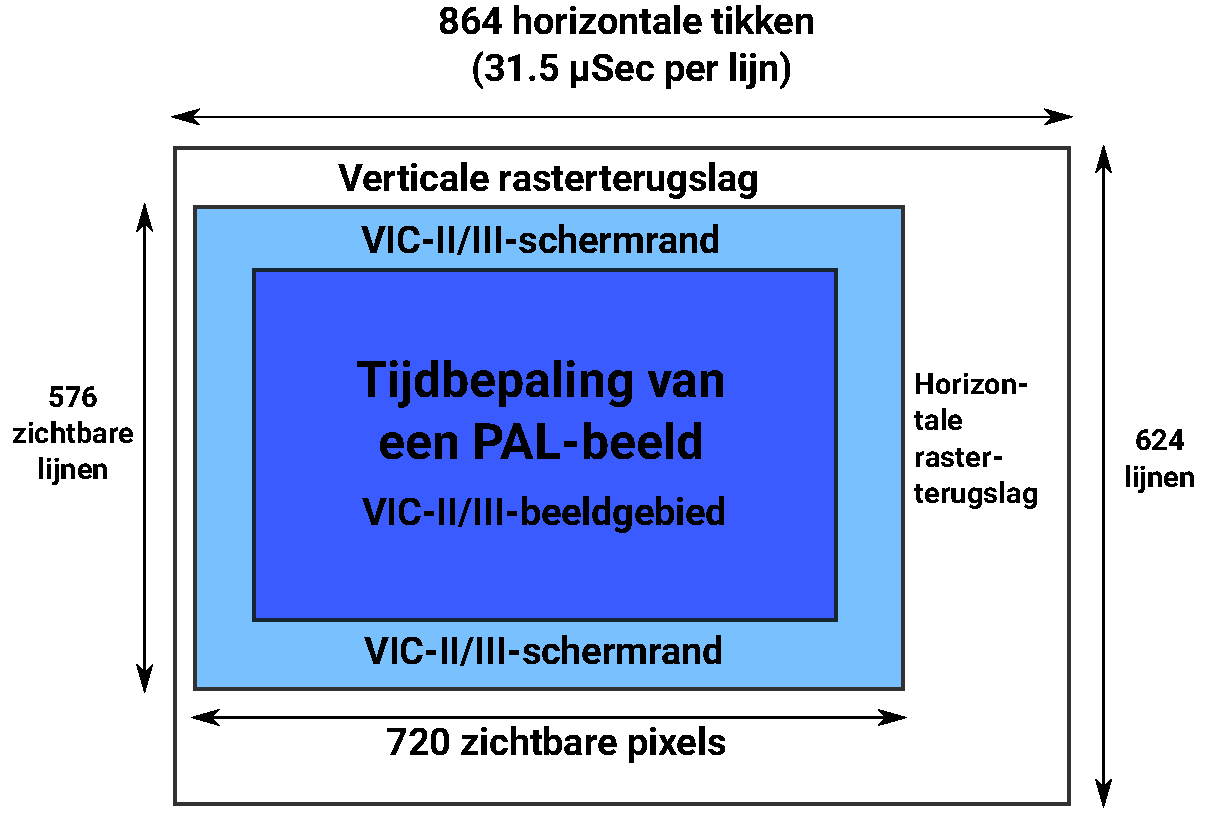
\includegraphics[width=\linewidth]{dutch/images/illustrations/VIC-IV-PAL-Frame.pdf}

Het NTSC-frame bestaat uit 526 fysieke rasterlijnen met elk 858 pixelklokken. De pixelklok is 27 MHz, oftewel 1/3 van de VIC-IV-pixelklok. Het zichtbare frame is 720$\times$480 pixels, waarvan het geheel in de VIC-IV-modus kan worden gebruikt. In de VIC-II- en VIC-III-modi verkleint het randgebied de bruikbare grootte tot 640$\times$400 pixels. In de VIC-II-modus en VIC-III 200H-modi wordt de weergave dubbelgescand, waarbij twee fysieke rasterlijnen van 32 microseconden overeenkomen met één VIC-II-stijl rasterlijn van 64 microseconden. Elk frame bestaat dus uit 263 VIC-II-rasterlijnen van elk 64 microseconden, overeenkomstig de meest voorkomende NTSC-videotiming van de C64.

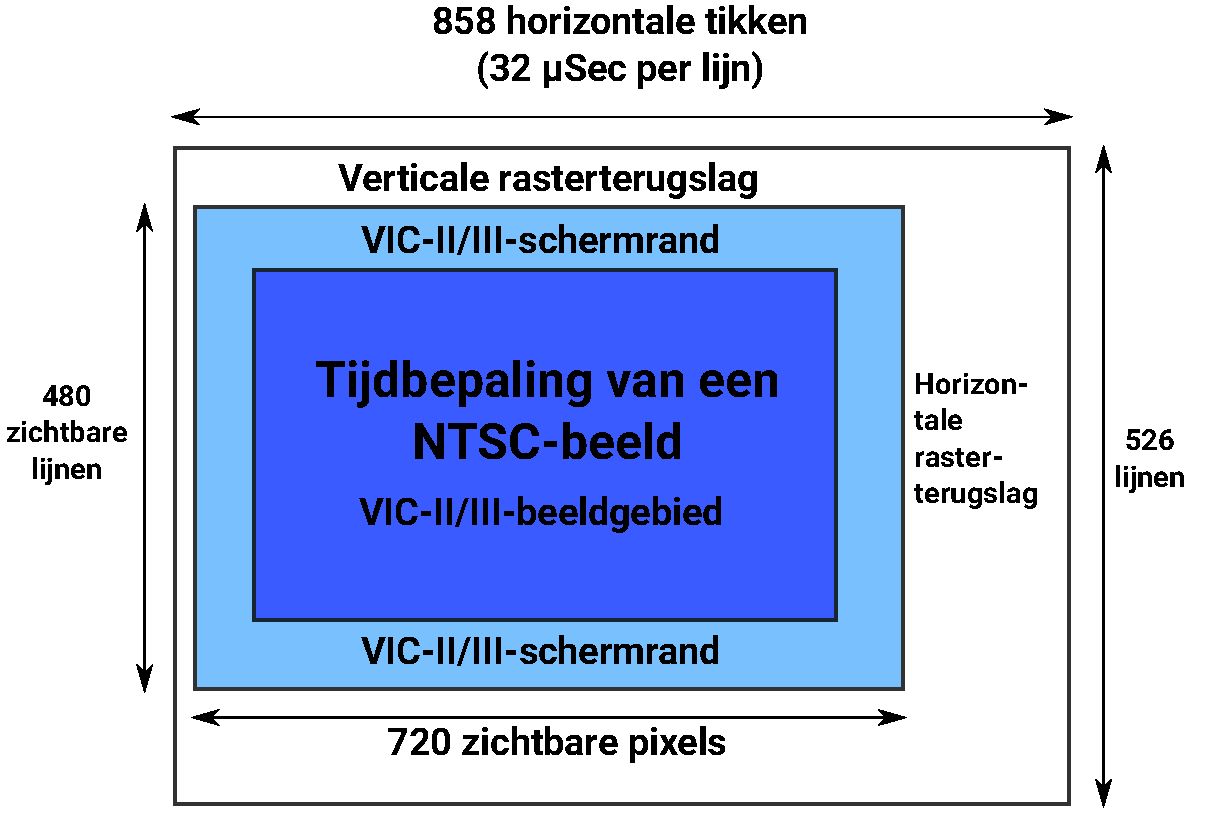
\includegraphics[width=\linewidth]{dutch/images/illustrations/VIC-IV-NTSC-Frame.pdf}

Omdat niet alle VGA-beeldschermen deze HDTV-videomodi ondersteunen, is er een compatibiliteitsmodus beschikbaar die een VGA-stijl modus van 640$\times$480 biedt. Omdat de pixelklok van de MEGA65 vaststaat op 27 MHz, werkt deze modus op 63 Hz. Dit zou op de overgrote meerderheid van VGA-beeldschermen moeten werken. Er zullen geen problemen optreden met de PAL/NTSC-modi bij gebruik van de digitale video-uitgang van de MEGA65 op de overgrote meerderheid van IMDH\texttrademark-compatibele beeldschermen en televisies.

Om te bepalen of de MEGA65 in PAL- of NTSC-modus werkt, kunt u het Freezer-menu openen, dat de huidige videomodus weergeeft, of vanuit een programma het PALNTSC-signaal controleren (bit 7 van \$D06F, decimaal 53359). Als deze bit gezet is, werkt het systeem in NTSC-modus; als deze gewist is, in PAL-modus. Deze bit kan worden gewijzigd om tussen de modi te schakelen, bijv.:

\begin{screencode}
10 REM C65+MEGA65-I/O INSCHAKELEN
20 IF PEEK($D018)<32 THEN POKE $D02F,ASC("G"):POKE $D02F,ASC("S")
30 REM NTSC-bit controleren
40 NTSC=PEEK($D06F) AND 128
50 REM STATUS WEERGEVEN EN OM OMSCHAKELING VRAGEN
60 PRINT"MEGA65 IS IN ";:IF NTSC THEN PRINT"NTSC MODE":ELSE PRINT"PAL MODE"
70 INPUT"SWITCH MODES (Y/N)? ",A$
80 REM NTSC-BIT OMSCHAKELEN
90 IF A$="Y" THEN POKE $D06F,PEEK($D06F) XOR 128:ELSE END
100 REM NIEUWE STATUS WEERGEVEN
110 NTSC=PEEK($D06F) AND 128
120 PRINT"MEGA65 IS IN ";:IF NTSC THEN PRINT"NTSC MODE":ELSE PRINT"PAL MODE"
\end{screencode}

\subsubsection{Fysieke en logische rasters}

Fysieke rasterlijnen per frame verwijzen naar het aantal daadwerkelijke rasterlijnen in de PAL- of NTSC-EDTV-videomodi die door de MEGA65 worden gebruikt. Logische rasterlijnen verwijzen naar het aantal VIC-II-stijl rasterlijnen per frame. Elke logische rasterlijn bestaat uit twee fysieke rasterlijnen per regel, aangezien EDTV-modi dubbelgescande modi zijn vergeleken met de oorspronkelijke PAL- en NTSC-SDTV-modi van de C64. De frame-parameters van de VIC-IV voor PAL en NTSC zijn als volgt:

\setlength{\tabcolsep}{3pt}
\begin{longtable}{|L{2cm}|L{2.5cm}|L{2.5cm}|L{2.5cm}|}
\hline
{\bf{Standaard}} & {\bf{Cycli per rasterlijn}} & {\bf{Fysieke rasterlijnen per frame}} & {\bf{Logische rasterlijnen per frame}}  \\
\hline
\endfirsthead
\multicolumn{3}{l@{}}{\ldots vervolg}\\
\hline
{\bf{Standaard}} & {\bf{Cycli per rasterlijn}} & {\bf{Fysieke rasterlijnen per frame}} & {\bf{Logische rasterlijnen per frame}}  \\
\hline
\endhead
\multicolumn{3}{l@{}}{vervolg \ldots}\\
\endfoot
\hline
\endlastfoot
	\small PAL & 63 & 626 & 312  \\	\small NTSC & 65 & 526 & 263  \\
\end{longtable}

Het resultaat is dat de frames op de VIC-IV exact hetzelfde aantal $\sim$1 MHz-CPU-cycli bevatten als op de VIC-II.

\subsubsection{Bad lines}

De VIC-IV kent van nature geen ``bad lines'', omdat de VIC-IV eigen geheugenbussen heeft naar het hoofdgeheugen en het kleurengeheugen (colour RAM) van de MEGA65. Hierdoor kunnen zowel de processor als de VIC-IV tegelijkertijd toegang krijgen tot het geheugen, in tegenstelling tot de C64 of C65, waarbij de toegang wordt afgewisseld.

Om de compatibiliteit te verbeteren, geeft de VIC-IV echter aan wanneer een ``bad line'' zou hebben plaatsgevonden op de VIC-II. De 45GS02-processor van de MEGA65 aanvaardt deze bad-line-signalen en onderbreekt de CPU gedurende 40 klokcycli, tenzij de processor op volle snelheid draait, in welk geval deze worden genegeerd. Dit verbetert de timingcompatibiliteit met de VIC-II aanzienlijk. De timing is echter niet exact, omdat de huidige revisie van de 45GS02 precies 40 cycli onderbreekt in plaats van 40--43 cycli, afhankelijk van de instructie die op dat moment wordt uitgevoerd. Daarnaast onderbreken de VIC-IV en 45GS02 momenteel niet voor sprite-ophaaloperaties.


De bad-line-emulatie wordt beheerd door bit 0 van \$D710: het zetten van deze bit schakelt bad-line-emulatie in, en het wissen ervan voorkomt dat een bad line tijd van de processor steelt.


\section{Geheugeninterface}

De VIC-IV ondersteunt tot 16 MB direct toegankelijk RAM voor videogegevens, maar momenteel bieden alle bestaande modellen slechts 384 KB adresseerbaar RAM. In MEGA65-systemen wordt het tweede blok van 128 KB RAM (in het geheugengebied van 128 KB tot 256 KB) doorgaans gebruikt om een C65-compatibele ROM op te slaan, waardoor 256 KB RAM voor de gebruiker beschikbaar blijft. Indien de software zo is geschreven dat het gebruik van C65-ROM-routines niet nodig is, kan de volledige 384 KB RAM door het programma worden gebruikt.

Alle MEGA65-modellen ondersteunen momenteel 32 KB kleurengeheugen (colour RAM), maar er zijn plannen om het nieuwste R3-bord 64 KB kleurengeheugen (of mogelijk zelfs 128 KB) te laten ondersteunen.

De VIC-IV ondersteunt alle methoden van de oudere VIC-II en VIC-III voor de toegang tot dit geheugen, waaronder het gebruik van 16KB-banken door de VIC-II en de Display Address Translator (DAT) van de VIC-III. Dit extra geheugen kan voor teken- en bitmapweergaven worden gebruikt, evenals voor sprites. De bitplanemodi van de VIC-III blijven echter beperkt tot het gebruik van slechts de eerste 128KB van het geheugen, omdat de VIC-IV de bitplanemodus niet uitbreidt.

\subsection{Schermgeheugen lokaliseren en verplaatsen}

De VIC kan worden geconfigureerd om het tekstschermgeheugen overal in de eerste 384KB te zoeken. Uw programma kan bepalen waar het schermgeheugen komt te staan en het startadres in de hardware-registers instellen. Dit adres wordt opgeslagen in de SCRNPTR-registers (\$D060 -- \$D063, 53344 -- 53347 decimaal). Om het schermgeheugen bijvoorbeeld op adres 12345 in te stellen:

\begin{screencode}
REM C65+MEGA65-I/O INSCHAKELEN
IF PEEK($D018)<32 THEN POKE $D02F,ASC("G"):POKE $D02F,ASC("S")

WPOKE $D060,$2345:POKE $D062,$1
\end{screencode}

Om een bestaand scherm te gebruiken dat door de KERNAL is ingesteld (het scherm dat de gebruiker bij het opstarten ziet), kunt u het startadres uit deze registers lezen. Houd er rekening mee dat de KERNAL in sommige omstandigheden de locatie van het schermgeheugen wijzigt. De beste praktijk is daarom dit adres binnen het programma uit de registers te lezen en de locatie ervan niet te veronderstellen.

\begin{screencode}
10 SC=WPEEK($D060)+(PEEK($D062)*65536)
20 POKE SC,1 : REM SCHRIJFT EEN "A" NAAR DE LINKERBOVENHOEK
\end{screencode}

\subsection{Tekengeneratorgegevens verplaatsen}

De locatie van de tekengeneratorgegevens kan eveneens met precisie op byteniveau worden ingesteld via de CHARPTR-registers op \$D068 -- \$D06A (53352 -- 53354 decimaal). Zoals gebruikelijk bevat het eerste van deze registers de minst significante byte en het laatste de meest significante byte. De drie bytes maken plaatsing van tekengeneratorgegevens overal in de eerste 16MB van het geheugen mogelijk. Voor systemen met minder dan 16MB geheugen waartoe de VIC-IV toegang heeft, dienen de bovenste adresbits op nul te staan.

Om bijvoorbeeld aan te geven dat de tekengeneratorgegevens vanaf \$41200 (266752 decimaal) moeten worden gelezen, kan het volgende worden gebruikt. Houd er rekening mee dat het commando WPOKE kan worden gebruikt om twee bytes als een woord naar een geheugen- of I/O-locatie te schrijven. Wij gebruiken daarom WPOKE om \$00 naar \$D068 en \$12 naar \$D069 te schrijven, en een extra POKE om de hoge byte \$A naar \$D06A te schrijven door het adres door 65536 te delen:

\begin{screencode}
REM C65+MEGA65-I/O INSCHAKELEN
IF PEEK($D018)<32 THEN POKE $D02F,ASC("G"):POKE $D02F,ASC("S")
REM HEX $41200 IS MAKKELIJK VERDEELD IN ZIJN 3 BYTES $00, $12, $4
REM WPOKE ZET DE ONDERSTE TWEE BYTES IN EEN COMMANDO EN
REM DE VOLGENDE POKE ZET DE BOVENSTE BYTE
A=$41200
WPOKE $D068,A
POKE $D06A,A/65536
\end{screencode}

\subsection{Het kleuren-/attribuutgeheugen verplaatsen}

Het gebruikte deel van het kleurengeheugen kan op vergelijkbare wijze worden ingesteld met de COLPTR-registers (\$D064 -- \$D065, 53348 -- 53349 decimaal). De waarde is namelijk een verschuiving vanaf het begin van het kleuren-/attribuutgeheugen. Dit komt omdat het kleuren-/attribuutgeheugen van de MEGA65, net als op de C64, een afzonderlijk geheugenonderdeel is met een eigen verbinding met de VIC-IV. Standaard zijn de COLPTR's op nul ingesteld, wat het gedrag van de VIC-II/III nabootst. Om de weergave het kleuren-/attribuutgeheugen vanaf verschuiving \$4000 te laten gebruiken, kan men bijvoorbeeld iets als het volgende gebruiken:

\begin{screencode}
REM C65+MEGA65-I/O INSCHAKELEN
IF PEEK($D018)<32 THEN POKE $D02F,ASC("G"):POKE $D02F,ASC("S")
REM STEL COLPTR IN OP $4000, VERDEELD IN $00-LSB en $40-MSB
POKE $D064,$00
POKE $D065,$40
\end{screencode}

\subsection{Spritepointers en sprite-afbeeldingen verplaatsen}

De locatie van de spritepointers kan eveneens worden verplaatst, en sprites kunnen hun gegevens overal in de eerste 4MB van het geheugen laten hebben. Dit wordt bereikt door eerst de locatie van de spritepointers in te stellen via de SPRPTRADR-registers (\$D06C -- \$D06E, 53356 -- 53358 decimaal; houd er echter rekening mee dat alleen de onderste 7 bits van \$D06E worden gebruikt, omdat de hoogste bit voor het SPRPTR16-signaal wordt gebruikt). Hierdoor kan de lijst van acht spritepointers van het einde van het schermgeheugen naar een willekeurige locatie in de eerste 8MB van het geheugen worden verplaatst. SPRPTRADR moet op een 16-byte-grens (een veelvoud van 16) zijn uitgelijnd.

Om sprites zelf overal in de eerste 4MB van het geheugen te kunnen plaatsen, moet de SPRPTR16-bit in \$D06E worden gezet. In deze modus worden twee bytes gebruikt om de locatie van elke sprite aan te geven, in plaats van één byte. De lijst van spritepointers is daardoor 16 bytes lang, in plaats van 8 bytes zoals op de VIC-II/III. Wanneer SPRPTR16 is ingeschakeld, moet de locatie van de spritepointers altijd expliciet via de SPRPTRADR-registers worden ingesteld.

Om de spritepointers bijvoorbeeld op locatie 800 -- 815 te plaatsen, kunt u min of meer de volgende code gebruiken. Houd er rekening mee dat enige kunstgrepen nodig zijn om de SPRPTR16-bit ongewijzigd te laten, en ook om de AND-binaire operator, die niet met waarden groter dan 65535 werkt, te omzeilen:

\begin{screencode}
REM C65+MEGA65-I/O INSCHAKELEN
IF PEEK($D018)<32 THEN POKE $D02F,ASC("G"):POKE $D02F,ASC("S")
POKE $D06C,(800-INT(800/65536)*65536) AND 255
POKE $D06D,INT(800/256) AND 255
POKE $D06E,(PEEK($D06E) AND 128)+INT(800/65536)
\end{screencode}

De locatie van elke sprite-afbeelding blijft een veelvoud van 64 bytes, waardoor er op elk moment tot 65,536 unieke sprite-afbeeldingen kunnen worden gebruikt, indien het systeem over voldoende geheugen beschikt (4MB of meer). In deze modus wordt de 16KB-banking van de VIC-II genegeerd, en is de locatie van de spritegegevens eenvoudigweg 64 $\times$ de pointerwaarde. Om de gegevens voor een sprite op \$C000 (49152 decimaal) te hebben, zou dit bijvoorbeeld sprite-locatie 768 zijn, omdat 49152 gedeeld door 64 = 768. Vervolgens moeten wij 768 in hoge en lage bytes splitsen om de twee pointerbytes in te stellen: 768 = 256$\times$3, met rest 0. Dit zou dus vereisen dat de twee spritepointerbytes 0 (lage byte, die als eerste komt) en 3 (hoge byte) zijn. Indien de spritepointers zich op \$7F8 (2040 decimaal) bevonden, zou het instellen van de eerste sprite op sprite-afbeelding 768 kunnen worden gedaan met zoiets als:

\begin{screencode}
POKE 2040,768-256*INT(768/256)
POKE 2041,INT(768/256)
\end{screencode}

\section{Hete registers}
\index{Hete registers}

Sommige VIC-IV-registers ondersteunen functies die vergelijkbaar zijn met die van de VIC-II en VIC-III, maar met uitgebreide mogelijkheden. Voor achterwaartse compatibiliteit zorgt het schrijven naar specifieke VIC-II- en VIC-III-registers er ook voor dat de bijbehorende VIC-IV-registers worden gereset met consistente waarden. Dit gedrag kan worden geconfigureerd met de HOTREG-vlag in bit 7 van \$D05D.

De onderste vier bits van register \$D018 (\textbf{CB}) stellen bijvoorbeeld het tekensetadres van de VIC-II in, als een veelvoud van 1 KiB. De VIC-IV kan de tekenset op elk 24-bits adres plaatsen met behulp van \$D06A (\textbf{CHARPTRBNK}), \$D068 (\textbf{CHARPTRLSB}) en \$D069 (\textbf{CHARPTRMSB}). Indien u CB instelt, worden de VIC-IV-registers ook bijgewerkt om hiermee overeen te komen.

De volledige reeks ``hete'' VIC-II-registers die van invloed zijn op de VIC-IV-registers omvat:

\begin{itemize}
\item \$D011 (53265): RB8, ECM, BMM, BLNK, RSEL, YSCL\item \$D016 (53270): RST, MCM, CSEL, XSCL\item \$D018 (53272): VS, CB\item \$D031 (53297): VIC-III-modi: H640, FAST, ATTR, BPM, V400, H1280, MONO, INT\item De VIC-II-bankbits van \$DD00 (56576) (CIA 2 PORTA)
\end{itemize}

Telkens wanneer een van die registers wordt gewijzigd, zelfs door de bestaande waarde er weer in terug te schrijven, worden alle bijbehorende VIC-IV-registers bijgewerkt op basis van de VIC-II-registerwaarden, zelfs die welke geen verband houden met het register waarnaar is geschreven. Dit omvat de FAST-vlag, welke zich op een byte-locatie van een heet register (\$D031) bevindt, maar geen verband houdt met de videoparameters en geen bijbehorend VIC-IV-register heeft.

De registers die tijdens dit proces worden gewijzigd, staan hieronder vermeld. Houd er rekening mee dat sommige van deze registers intern zijn aan de VIC-IV en niet rechtstreeks door de gebruiker kunnen worden opgevraagd of gewijzigd. Waar dit het geval is, worden er geen adressen voor de registers vermeld.

\begin{itemize}
\item {\bf X-positie van de linkerrandgrens.}  Dit interne register wordt bijgewerkt om de linkerrand in te stellen op de breedte die in de ``Single Side Border Width''-registers is aangegeven (\$D05C bevat de LSB, en bits 0 -- 5 van \$D05D bevatten de MSB van de breedte van de zijrand.  Houd er rekening mee dat de breedte van de zijrand is gebaseerd op de afmetingen van het videoframe op laag niveau, niet op de weergavegrootte van het scherm van de videomodus. Wanneer het 38/40-kolommenveld van \$D016 op 38 kolommen is ingesteld, verschijnt de linkerrandgrens 14 pixels rechts van zijn normale positie.\item {\bf X-positie van de rechterrandgrens.} Dit is hetzelfde als de linkerrandgrens, maar dan voor de rechterrand van het scherm. Houd er rekening mee dat wanneer de 38/40-kolommenvlag op 38 kolommen is ingesteld, de rechterrandgrens 17 pixels naar links van zijn normale positie wordt verplaatst.\item {\bf Y-positie van de bovenste randgrens (\$D048 LSB, bits 0 -- 3 van \$D049 MSB).} Dit interne register wordt ingesteld op de normale bovenste positie van het scherm, minus de waarde van het RASLINE0-veld in bits 0 -- 5 van \$D06F.  Wanneer het 24/25-rijenveld van \$D011 op 24 rijen is ingesteld, wordt de bovenste randgrens met 8 rasterlijnen verlaagd.\item {\bf Y-positie van de onderste randgrens (\$D04A LSB, bits 0 -- 3 van \$D04B MSB).} Dit interne register wordt ingesteld op de normale bovenste positie van het scherm, plus 400 rasterlijnen, om het normale 400px hoge primaire weergavegebied binnen de randen te creëren. Wanneer het 24/25-rijenveld van \$D011 op 24 rijen is ingesteld, wordt de bovenste randgrens met 8 rasterlijnen verhoogd.\item {\bf Verticale schaal van de tekengenerator (\$D05B).} Dit register wordt ingesteld op 0 voor de V200- of 1 voor de V400-modus, zodat elke pixelrij in een teken respectievelijk 1 of 2 pixels hoog wordt, volgens de V400-vlag.\item {\bf Aantal weer te geven tekenrijen (\$D07B).} Dit register wordt ingesteld op 25-1 = 24 of 50-1 = 49 om respectievelijk 25 of 50 tekstrijen weer te geven.  Houd er rekening mee dat wanneer \$D011 wordt gebruikt om de verticale randen naar binnen te brengen om het aantal zichtbare tekenrijen te verminderen, de VIC-IV nog steeds alle 25 of 50 rijen tekent.\item {\bf X-positie waar de tekenweergave begint (\$D04C LSB, bits 0 -- 3 van \$D04D MSB).}  Dit register wordt ingesteld op een positie ten opzichte van de rand van het 40-kolommen brede tekstscherm, plus 2$\times$ de positie van de vloeiende verschuiving die in \$D016 is aangegeven.\item {\bf Y-positie waar de tekenweergave begint (\$D04E LSB, bits 0 -- 3 van \$D04F MSB).}  Dit register wordt ingesteld op de bovenrand van de verticale rand, minus het VIC-II First Raster-aanpassingsregister (bits 0 -- 5 van \$D06F), plus eventuele verschuiving als gevolg van de verticale bits voor vloeiende verschuiving in \$D011.\item {\bf Virtuele rijbreedte (\$D058 LSB, \$D059 MSB), d.w.z. het aantal bytes scherm- en kleurengeheugen waarmee de VIC-IV vooruitgaat bij het weergeven van elke opeenvolgende tekenrij.} Dit register wordt ingesteld op 40 als de H640-vlag is gewist, of op 80 als de H640-vlag is gezet, waardoor de voortgang overeenkomt met het aantal weer te geven tekens.\item {\bf Breedte van de weergaverij (\$D05E LSB, bits 4 -- 5 van \$D063 MSB).} Dit register wordt ingesteld op 40 als de H640-vlag is gewist, of op 80 als de H640-vlag is gezet.\item {\bf Basisadres van het schermgeheugen (\$D060 -- \$D062, dat een 24-bits adres voorstelt).}  Dit adres wordt gereset naar het adres zoals berekend aan de hand van \$D018 en \$DD00, zoals op de C64.\item {\bf Spritepointer-adres van de VIC-II (\$D06C -- \$D06E, dat een 24-bits adres voorstelt).} Dit register wordt gereset naar de normale locatie aan het einde van het schermgeheugen van de huidige modus.  Indien de H640-vlag is gezet, gebeurt dit aan het einde van het 2KB-gebied van het schermgeheugen, of indien de H640-vlag niet is gezet, wijst het naar het einde van het 1KB-gebied van het schermgeheugen, zoals op een C64.\item {\bf Basisadres van de tekenset (\$D068 -- \$D06A, dat een 24-bits adres voorstelt).}  Houd er rekening mee dat de hete registerfunctie alleen de onderste 16 bits van het tekensetadres instelt. Dat wil zeggen dat \$D06A niet wordt gewist. Dit is bewust gedrag, waardoor het gemakkelijker wordt om in bestaande VIC-II-georiënteerde software de tekenset te vervangen door een andere tekenset in een andere geheugenbank.\item {\bf Basisadres van het kleurengeheugen (\$D064 LSB, \$D065 MSB).} Deze registers worden naar nul gereset, waardoor de VIC-IV verwacht dat het kleurengeheugen voor het scherm zich in het eerste deel van het kleurengeheugen bevindt, om compatibel te zijn met de VIC-II en VIC-III.
\end{itemize}

Dit gedrag van de VIC-II-registers is vooral bedoeld voor software uit het verleden die geen weet heeft van (en daarom nooit naar) VIC-IV-registers schrijft. De hete-registerpropagatie kan worden uitgeschakeld door het HOTREG- (``hete register'') signaal te wissen: bit 7 van \$D05D (53341). Indien u de HOTREG-vlag wist, moet u de VIC-IV-registers rechtstreeks bijwerken wanneer u de parameters van de videomodus wilt wijzigen.

Indien u een wijziging in een heet register aanbrengt terwijl HOTREG is uitgeschakeld en HOTREG vervolgens weer inschakelt, worden alle hete registers onmiddellijk bijgewerkt. Er zijn zeldzame gevallen waarin u een wijziging in een heet register wilt aanbrengen zonder de VIC-IV-registers bij te werken, maar de hete registers na de wijziging toch ingeschakeld wilt hebben. Om dit te doen, kunt u de openstaande bijwerking annuleren door vlak voordat u de hete registers weer inschakelt opnieuw een 0 naar HOTREG te schrijven. De volledige procedure is:

\begin{enumerate}
\item Schrijf 0 naar HOTREG om hete registers uit te schakelen.\item Werk het VIC-II-register bij dat u wilt wijzigen.\item Schrijf 0 naar HOTREG om de openstaande bijwerking te annuleren.\item Schrijf 1 naar HOTREG om hete registers weer in te schakelen.
\end{enumerate}

In assembleertaal:

\begin{screencode}
lda #%10000000
trb $d05d        ; hete registers uitschakelen

lda #%01000000
tsb $d031        ; een VIC-II/III-register bijwerken

lda #%10000000
trb $d05d        ; openstaande bijwerking wissen
tsb $d05d        ; hete registers weer inschakelen
\end{screencode}


\section{Nieuwe modi}

\subsection{Waarom de nieuwe VIC-IV-modi teken- en bitmapmodi zijn en geen bitplanemodi}

De nieuwe videomodi van de VIC-IV zijn afgeleid van de teken- en bitmapmodi van de VIC-II, in plaats van de bitplanemodi van de VIC-III. Deze keuze was gebaseerd op diverse praktische aspecten van het programmeren van een geheugenbeperkte 8-bit thuiscomputer:

\begin{enumerate}
\item Bitplanes vereisen dat dezelfde hoeveelheid geheugen aan elk gebied op het scherm wordt toegewezen, ongeacht of het lege ruimte of complexe afbeeldingen weergeeft. Met bitplanes is het niet mogelijk om inhoud uit een afbeelding opnieuw te gebruiken in een ander deel van die afbeelding. De meeste C64-spellen maken echter gebruik van sterk repetitieve schermen, waarbij veelgebruikte elementen op diverse plaatsen op het scherm voorkomen, waarvan Boulder Dash en Super Giana Sisters goede voorbeelden zijn.

\item Bitplanes maken het ook moeilijk om een beeldscherm bij te werken, omdat elke pixel uniek is: er is geen mogelijkheid om een wijziging, bijvoorbeeld in de animatie van een schermelement, door te voeren op alle plaatsen tegelijk. De diamantanimaties in Boulder Dash zijn een goed voorbeeld van dit probleem. Het moeten wijzigen van meerdere afzonderlijke bytes in elke bitplane vormt een verhoogde rekenkundige belasting, hetgeen de reden was dat er voor de Amiga AAA-chipset werd gevraagd zogenaamde ``chunky''-modi op te nemen, in plaats van uitsluitend op bitplanes gebaseerde modi. Hoewel de Display Address Translator (DAT) en DMAgic van de C65 enige verlichting bieden voor dit probleem, is die verlichting slechts gedeeltelijk.

\item Scrollen met behulp van de bitplanes van de C65 vereist het kopiëren van de gehele bitplane, omdat de hardwareondersteuning voor vloeiend scrollen zich niet uitstrekt tot het op fijne wijze wijzigen van het bronadres van de bitplane. Zelfs met gebruikmaking van de DMAgic vereist het scrollen van een 320$\times$200 256-kleurenscherm in het gunstigste geval 128.000 klokcycli (het lezen en schrijven van 320$\times$200 = 64.000 bytes). Op 3.5 MHz op de C65 zou dit ongeveer 36 milliseconden kosten, oftewel ongeveer 2 volledige videoframes. Voor vloeiend scrollen van een dergelijk scherm is daarom een dubbelgebufferde regeling nodig, die 128.000 van de 131.072 bytes geheugen zou verbruiken.

De bekende tekenmodi van de VIC-II worden daarentegen veelvuldig in spellen gebruikt, omdat ze met een geringe hoeveelheid schermgeheugen kunnen bepalen welk blok van 8$\times$8 pixels wordt weergegeven, wat zeer snel scrollen, minder geheugengebruik en effectieve hardwareversnelling van animatie van veelgebruikte elementen mogelijk maakt. De verbeteringen in de VIC-IV zijn dan ook vooral op de tekenmodus gericht. Omdat de bitmapmodus op de VIC-II feitelijk een speciaal geval van de tekenmodus is, met impliciete tekennummers, wordt deze op de VIC-IV als het ware gratis meegeleverd en zal alleen in het kader van een zeer klein aantal bitmapmodus-specifieke verbeteringen worden genoemd die triviaal te implementeren waren en waarvan het dus onverstandig leek ze niet te realiseren, voor het geval ze toch van pas komen.

\end{enumerate}

\subsection{Weergeven van meer dan 256 unieke tekens via ``Super-Uitgebreide Attribuutmodus''}

De belangrijkste innovatie is de toevoeging van de Super-Uitgebreide Attribuutmodus (SEAM). De VIC-II gebruikt al 12 bits per teken: elke cel van 8$\times$8 pixels wordt gedefinieerd door 12 bits gegevens: 8 bits schermgeheugengegevens, standaard van \$0400 -- \$07E7 (1024 -- 2023 decimaal), die aangeven welke tekens moeten worden weergegeven, en 4 bits kleurgegevens van het 1 KB nibble kleurengeheugen op \$D800 -- \$DBFF (55296 -- 56319 decimaal). De VIC-III van de C65 gebruikt 16 bits, omdat het kleurengeheugen nu 8 bits telt in plaats van 4, waarbij de extra 4 bits kleurengeheugen worden gebruikt om attributen te ondersteunen (knipperen, vet, onderstrepen en inverse weergave). Het wordt aanbevolen om de werking hiervan door te nemen voordat u verder leest. Een goede inleiding op de tekstmodus van de VIC-II is op veel plaatsen te vinden.
% For example, \ref{vicii-cheaper-by-the-dozen}. <- undefined
Super-Uitgebreide Attribuutmodus verdubbelt het aantal bits per teken van de 16 van de VIC-III tot 32: twee bytes schermgeheugen en twee bytes kleuren-/attribuutgeheugen.

Super-Uitgebreide Attribuutmodus wordt ingeschakeld door bit 0 in \$D054 (53332 decimaal) te zetten. Vergeet niet eerst de VIC-IV-modus in te schakelen om dit register toegankelijk te maken. Wanneer deze bit is gezet, worden twee bytes gebruikt voor zowel het schermgeheugen als het kleurengeheugen voor elk teken dat op het scherm wordt weergegeven. In vergelijking met de 12 bits informatie die de C64 per teken gebruikt en de 16 bits van de VIC-III, heeft de VIC-IV 32 bits informatie. Hoe deze 32 bits worden gebruikt, varieert enigszins per modus, zoals beschreven in de volgende tabellen, inclusief of de GOTOX-bit is gezet.

Let er ook op dat het tegelijkertijd inschakelen van de BOLD- en REVERSE-attributen op de MEGA65 een alternatief palet selecteert, waardoor feitelijk 512 kleuren op het scherm mogelijk zijn, maar elk 8$\times$8-teken slechts kleuren uit één palet van 256 kleuren kan gebruiken.

De twee tabellen die volgen beschrijven de bitvelden die voor dit teken beschikbaar zijn, die variëren afhankelijk van of de \textbf{GOTOX\_flag} is gezet of gewist:

\begin{itemize}
  \item \textbf{GOTOX\_flag = 0} creëert een \underline{zichtbaar teken} (\textcolor{blue}{blauwe} bitvelden) met attributen die \underline{dit teken} beïnvloeden.  \item \textbf{GOTOX\_flag = 1} creëert een \underline{onzichtbaar teken} (\textcolor{red}{rode} bitvelden) met attributen die \underline{volgende tekens} beïnvloeden.
\end{itemize}


% Force table to sit on a single page for more convenient reading.
% ensures that they are both visible on the same open page :)
% (\cleardoublepage does the opposite)
\clearpage
\ifodd\value{page}\hbox{}\newpage\fi
\subsubsection{Bitvelden indien GOTOX\_flag is gewist:}

\setlength{\tabcolsep}{3pt}
\begin{longtable}{|L{2.1cm}|L{9cm}|}
  \hhline{==}
  {\bf{Bit(s)}} & {\bf{Functie wanneer GOTOX\_flag is \underline{\textcolor{blue}{gewist}}}}  \\
  \hhline{==}
\endfirsthead
\multicolumn{2}{l@{}}{\ldots vervolg}\\
  \hhline{==}
  {\bf{Bit(s)}} & {\bf{Functie wanneer GOTOX\_flag is \underline{\textcolor{blue}{gewist}}}}  \\
  \hhline{==}
\endhead
\multicolumn{2}{l@{}}{vervolg \ldots}\\
\endfoot
\hline
\endlastfoot
  \hline
  \multicolumn{2}{|l|}{\small \textbf{Schermgeheugen-byte 0}} \\
  \hline
  \small \qquad Bits 7 - 0 & {\small \textbf{\textcolor{blue}{char\_number (lo)}}: (bits 7 -- 0) Laagste byte van tekennummer\newline  (hetzelfde als de VIC-II en VIC-III) }\\
  \hline
  \multicolumn{2}{|l|}{\small \textbf{Schermgeheugen-byte 1}} \\
  \hline
  \small \qquad Bits 7 -- 5 & {\small \textbf{\textcolor{blue}{rhs\_trim (lo)}}: (bits 2 -- 0) Pixels aan de rechterkant van het teken wegsnijden)}\\
  \hline
  \small \qquad Bits 4 - 0 & {\small \textbf{\textcolor{blue}{char\_number (hi)}}: (bits 12 -- 8) Bovenste 5 bits van tekennummer, waardoor 8.192 unieke tekens kunnen worden aangesproken }\\
  \hline
  \multicolumn{2}{|l|}{\small \textbf{Kleurengeheugen-byte 0}} \\
  \hline
  \small \qquad Bit 7 & {\small \textbf{\textcolor{blue}{vert\_flip}}: het teken verticaal spiegelen }\\
  \hline
  \small \qquad Bit 6 & {\small \textbf{\textcolor{blue}{horz\_flip}}: het teken horizontaal spiegelen }\\
  \hline
  \small \qquad Bit 5 & {\small \textbf{\textcolor{blue}{alpha\_mode}}: de alpha-blendmodus inschakelen. De pixelwaarden worden dan als alpha-waarden behandeld die tussen de voorgrondkleur en de achtergrondkleur mengen (hiervoor moet \$D054.7 - ALPHEN worden ingesteld) }\\
  \hline
  \small \qquad \textbf{Bit 4} & {\small \textbf{GOTOX\_flag} is \textbf{\underline{\textcolor{blue}{gewist}} (op 0 gesteld)} \linebreak Verschaft de \textcolor{blue}{blauwe} bitvelden die in deze tabel worden getoond. Dit zijn attributen die invloed hebben op \underline{dit teken}. }\\
  \hline
  \small \qquad Bit 3 & {\small \textbf{\textcolor{blue}{ncm\_flag}}:
\begin{itemize}
  \item 1 = \underline{NCM-teken}: gebruikt 4 bits per pixel en is 16 pixels breed (minus eventuele trim-bits aan de rechterkant)  \item 0 = \underline{FCM-teken}: gebruikt 8 bits per pixel en is 8 pixels breed (minus eventuele trim-bits aan de rechterkant)
\end{itemize} }\\
  \hline
  \small \qquad Bit 2 & {\small \textbf{\textcolor{blue}{rhs\_trim (hi)}}: (bit 3) pixels aan de rechterkant van het teken wegsnijden}\\
  \hline
\small \qquad Bits 1 -- 0 & {\small GERESERVEERD, op 0 gesteld }\\
  \hline
  \multicolumn{2}{|l|}{\small \textbf{Kleurengeheugen-byte 1}} \\
  \hline
  \multicolumn{2}{|l|}{\small \quad \underline{Indien de VIC-II-multicolourmodus is ingeschakeld}: (\$D016.4 - MCM)} \\
  \hline
  \small \qquad Bits 7 -- 4 & {\small \textbf{\textcolor{blue}{colour (hi)}}: bovenste 4 bits van de voorgrondkleur van het teken}\\
  \hline
  \multicolumn{2}{|l|}{\small \quad \underline{Indien de uitgebreide attributen van de VIC-III zijn ingeschakeld}: (\$D031.5 - ATTR)} \\
  \hline
  \small \qquad Bit 7 & {\small \textbf{\textcolor{blue}{underline}}: Hardwarematige onderstreping van het teken }\\
  \hline
  \small \qquad Bit 6 & {\small \textbf{\textcolor{blue}{bold}}: Vetattribuut van het teken (hardware) * }\\
  \hline
  \small \qquad Bit 5 & {\small \textbf{\textcolor{blue}{reverse}}: Omgekeerde weergave van het teken (hardware) * }\\
  \hline
  \small \qquad Bit 4 & {\small \textbf{\textcolor{blue}{blink}}: Knipperen van het teken (hardware)}\\
  \hline
  \multicolumn{2}{|l|}{\small \quad \underline{Het overgebleven bitveld is gemeenschappelijk}:} \\
  \hline
\small \qquad Bits 3 -- 0 & {\small \textbf{\textcolor{blue}{colour (lo)}}: onderste 4 bits van de voorgrondkleur van het teken }\\
\end{longtable}

% Force table to sit on a single page for more convenient reading.
\newpage
\subsubsection{Bitvelden indien GOTOX\_flag is ingesteld:}

\setlength{\tabcolsep}{3pt}
\begin{longtable}{|L{2.1cm}|L{9cm}|}
  \hhline{==}
  {\bf{Bit(s)}} & {\bf{Functie wanneer GOTOX\_flag is \underline{\textcolor{red}{ingesteld}}}}  \\
  \hhline{==}
\endfirsthead
\multicolumn{2}{l@{}}{\ldots vervolg}\\
  \hhline{==}
  {\bf{Bit(s)}} & {\bf{Functie wanneer GOTOX\_flag is \underline{\textcolor{red}{ingesteld}}}}  \\
  \hhline{==}
\endhead
\multicolumn{2}{l@{}}{vervolg \ldots}\\
\endfoot
\hline
\endlastfoot
  \hline
  \multicolumn{2}{|l|}{\small \textbf{Schermgeheugen-byte 0}} \\
  \hline
  \small \qquad Bits 7 - 0 & {\small \textbf{\textcolor{red}{gotox\_pos (lo)}}: (bits 7 -- 0) onderste 8 bits van de nieuwe X-positie waar \underline{volgende tekens} moeten beginnen met tekenen, ten opzichte van het begin van het tekenen van het teken.  Door dit op 0 te stellen wordt het volgende teken over het meest linkse teken heen getekend. }\\
  \hline
  \multicolumn{2}{|l|}{\small \textbf{Schermgeheugen-byte 1}} \\
  \hline
  \small \qquad Bits 7 - 5 & {\small \textbf{\textcolor{red}{fcm\_yoffs}}: Y-offset van FCM-tekengegevens: wanneer niet nul, worden FCM-tekengegevens opgehaald vanaf het tekenadres + 8 $\times$ de Y-waarde, wat equivalent is aan één pixellijn FCM-tekengegevens per Y. Door zorgvuldig plannen kan dit worden gebruikt om meerdere lagen RRB-inhoud soepel verticaal te scrollen.  }\\
  \hline
  \small \qquad Bit 4 & {\small \textbf{\textcolor{red}{fcm\_yoffs\_dir}}: wanneer ingesteld, wordt het \textbf{\textcolor{red}{fcm\_yoffs}}-veld in plaats daarvan in mindering gebracht. }\\
  \hline
\small \qquad Bits 3 - 2 & {\small GERESERVEERD, op 0 ingesteld }\\
  \hline
  \small \qquad Bits 1 - 0 & {\small \textbf{\textcolor{red}{gotox\_pos (hi)}}: (bits 9 -- 8) bovenste 2 bits van de nieuwe X-positie (het hoogste bit is het tekenbit van het tweecomplement) }\\
  \hline
  \multicolumn{2}{|l|}{\small \textbf{Kleurengeheugen-byte 0}} \\
  \hline
  \small \qquad Bit 7 & {\small \textbf{\textcolor{red}{transparent\_flag}}: wanneer ingesteld, worden achtergrond-/transparante pixels niet getekend voor \underline{volgende tekens}, waardoor lagen mogelijk zijn }\\
  \hline
  \small \qquad Bit 6 & {\small \textbf{\textcolor{red}{background\_flag}}: wanneer ingesteld, worden \underline{volgende tekens} als achtergrond gerenderd, waardoor sprites ervoor kunnen verschijnen, zelfs wanneer sprites op achtergrond zijn ingesteld. }\\
  \hline
\small \qquad Bit 5 & {\small GERESERVEERD, op 0 ingesteld }\\
  \hline
  \small \qquad \textbf{Bit 4} & {\small \textbf{GOTOX\_flag} is \textbf{\textcolor{red}{op 1 ingesteld}}. Biedt de in deze tabel getoonde \textcolor{red}{rode} bitvelden, dit zijn attributen die \underline{volgende tekens} beïnvloeden. Eén opvallend veld is \textbf{\textcolor{red}{gotox\_pos}}, dat later in de sectie Raster-Rewrite Buffer wordt besproken.)}\\
  \hline
  \small \qquad Bit 3 & {\small \textbf{\textcolor{red}{rowmask\_flag}}: wanneer ingesteld, beslist het \textbf{\textcolor{red}{rowmask}}-veld welke pixellijnen van \underline{volgende tekens} moeten worden gerenderd. Dit kan worden gebruikt om tekens verticaal te scrollen met RRB, door elk teken op twee rijen te tekenen: verschoven naar beneden op de bovenste rij, en verschoven omhoog op de onderste rij, en gemaskeerd zodat alleen de pixellijnen van het gescrollde teken worden weergegeven, en niet de gegevens van vóór/na de gegevens van dat teken.}\\
  \hline
  \small \qquad Bit 2 & {\small \textbf{\textcolor{red}{foreground\_flag}}: wanneer ingesteld, worden \underline{volgende tekens} als voorgrond getekend, ongeacht hun kleur, waardoor sprites erachter kunnen verschijnen. }\\
  \hline
\small \qquad Bits 1 - 0 & {\small GERESERVEERD, op 0 ingesteld }\\
  \hline
  \multicolumn{2}{|l|}{\small \textbf{Kleurengeheugen-byte 1}} \\
  \hline
  \small \qquad Bits 7 - 0 & {\small \textbf{\textcolor{red}{rowmask}}: maskerwaarden voor pixellijnen. Bits 7 -- 0 = Rijen 7 -- 0.\newline 1 = rij weergeven, 0 = rij verbergen }\\
\end{longtable}


We zien dat we nog steeds de onderste 8 bits van het tekennummer in de C64-stijl hebben in de eerste schermgeheugen-byte. De tweede byte van het schermgeheugen krijgt daarvoor vijf extra bits, waardoor er 2$^{13}$ = 8.192 verschillende tekens op één scherm kunnen worden gebruikt. Dat is meer dan voldoende voor unieke tekens die een 80$\times$50-scherm bestrijken (wat mogelijk is om te maken met de VIC-IV).  De resterende bits maken het bijsnijden van het teken mogelijk.  Hierdoor kunnen tekens met variabele breedte worden gebruikt, waarmee dingen gedaan kunnen worden die normaal niet mogelijk zouden zijn, zoals het gebruik van tekstmodus voor vrije horizontale plaatsing van tekens (of delen daarvan). Dit werd oorspronkelijk toegevoegd om hardwarematige ondersteuning voor proportionele breedte-lettertypen mogelijk te maken.

Voor het kleurengeheugen is de tweede byte (byte 1) gelijk aan die van de C65, oftewel de onderste helft biedt vier bits voor de voorgrondkleur, zoals op de C64, plus de optionele VIC-III uitgebreide attributen. Het C65-specificatiedocument beschrijft het gedrag wanneer meer dan één van deze tegelijk wordt gebruikt, waarvan de meeste logisch zijn, maar er zijn een paar combinaties die zich anders gedragen dan verwacht. Het combineren van vetgedrukt met knipperen zorgt er bijvoorbeeld voor dat het teken schakelt tussen de vetgedrukte en de normale modus. Vetgedrukte modus zelf wordt geïmplementeerd door effectief te fungeren als bit 4 van de voorgrondkleurwaarde, waardoor de kleur van andere paletposities wordt getekend dan normaal.

Indien u de VIC-III uitgebreide attributen niet nodig heeft, kunt u in plaats daarvan de bovenste vier bits van de tweede byte van het kleurengeheugen gebruiken om meer bits van de kleurindex te bevatten, waardoor een selectie uit het volledige bereik van 256 kleurinstellingen mogelijk is.  Deze modus wordt geactiveerd door de multicolourmodus van de VIC-II in te schakelen terwijl de volledige kleurmodus actief is.

De C65 / VIC-III-attributen en het gebruik van 256-kleuren 8-bit-waarden voor verschillende VIC-II-kleurregisters wordt ingeschakeld door bit 5 van \$D031 (53297 decimaal) in te stellen.  Het wordt sterk aanbevolen dit te doen bij het gebruik van de VIC-IV-modus, omdat anders bepaalde functies niet naar behoren werken. Merk op dat BOLD+REVERSE samen de betekenis heeft van het selecteren van een alternatief palet op de MEGA65, wat verschilt van de C65.

Dankzij Super-Uitgebreide Attribuutmodus zijn veel effecten mogelijk.  Een paar mogelijkheden worden in de volgende subsecties uitgelegd.

\subsection{Super-Uitgebreide Attribuutmodus gebruiken}

Super-Uitgebreide Attribuutmodus vereist twee keer zoveel schermgeheugen en kleurengeheugen als de VIC-II/III-tekstmodi. Dit komt doordat er twee bytes van elk nodig zijn om elk teken te definiëren, in plaats van één.  Het schermgeheugen kan op elke willekeurige locatie in het 384KB hoofdgeheugen worden geplaatst met behulp van de registers \$D060 -- \$D062 (53344 -- 53346 decimaal).  Het kleurengeheugen kan op elke willekeurige locatie in het 32KB kleurengeheugen worden geplaatst.  Alleen de eerste 1 of 2KB van het kleurengeheugen is zichtbaar op \$D800 -- \$DBFF of \$D800 -- \$DFFF (indien het {\em CRAM2K}-signaal is ingesteld in bit 0 van \$D030, 53296 decimaal).  Indien een scherm groter dan 40$\times$25 tekens wordt gebruikt, is het gebruik van de DMA-controller of een andere manier vereist om het volledige kleurengeheugen te benaderen.  We bespreken daarom eerst het gebruik van Super-Uitgebreide Attribuutmodus met een 40x25-tekenweergave.

De eerste stap is het inschakelen van Super-Uitgebreide Attribuutmodus door de {\em FCLRHI}- en {\em CHR16}-signalen te activeren, door bits 2 en 0 van \$D054 (53332 decimaal) in te stellen.  Aangezien dit een VIC-IV-register is, moet eerst de VIC-IV I/O-modus worden ingeschakeld.  De VIC-IV moet ook worden geconfigureerd naar 40-kolomsmodus, door het {\em H640}-signaal uit te schakelen door bit 7 van \$D031 (53297 decimaal) te wissen.  Dit komt doordat elk tekenpaar samen één teken op het scherm vormt, waarbij één teken twee schermgeheugenbytes vereist, waardoor er 80 schermgeheugenbytes nodig zijn om 40 tekens weer te geven.  Eveneens zijn er 80 kleurengeheugenbytes nodig.

Om dit visueel te begrijpen, is het nuttig eerst de normale C64-schermgeheugenindeling te bekijken:

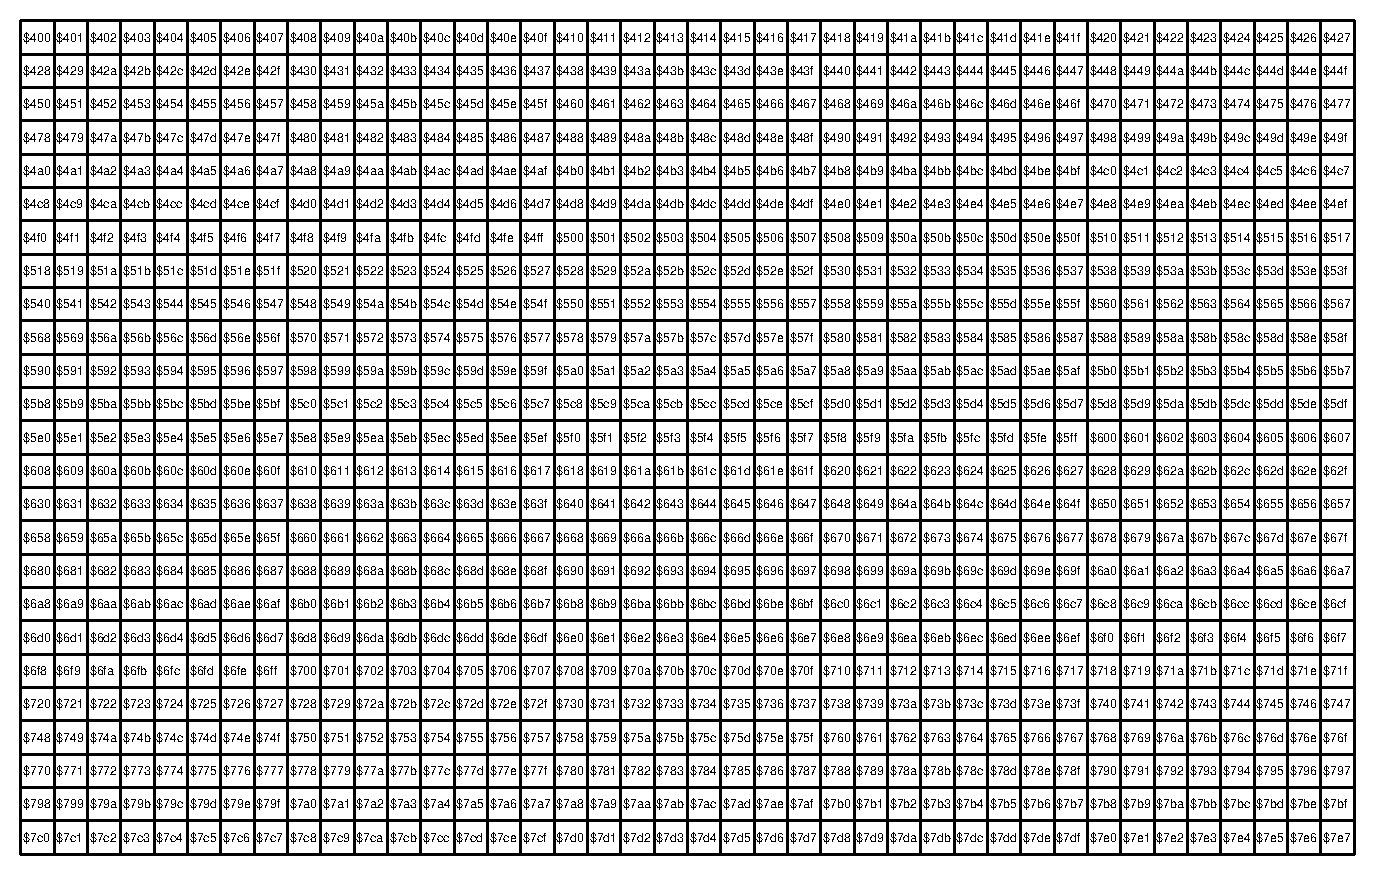
\includegraphics[width=\linewidth]{images/illustrations/screen-40x25-addresses.pdf}

Dat wil zeggen: elk tekencel gebruikt één byte van het schermgeheugen en de adressen nemen geleidelijk toe, zowel binnen regels als tussen regels. Super-Uitgebreide Attribuutmodus vereist twee bytes per tekencel. Indien u \$D054 bijvoorbeeld op \$05 instelt, krijgt u schermadressen als volgt:

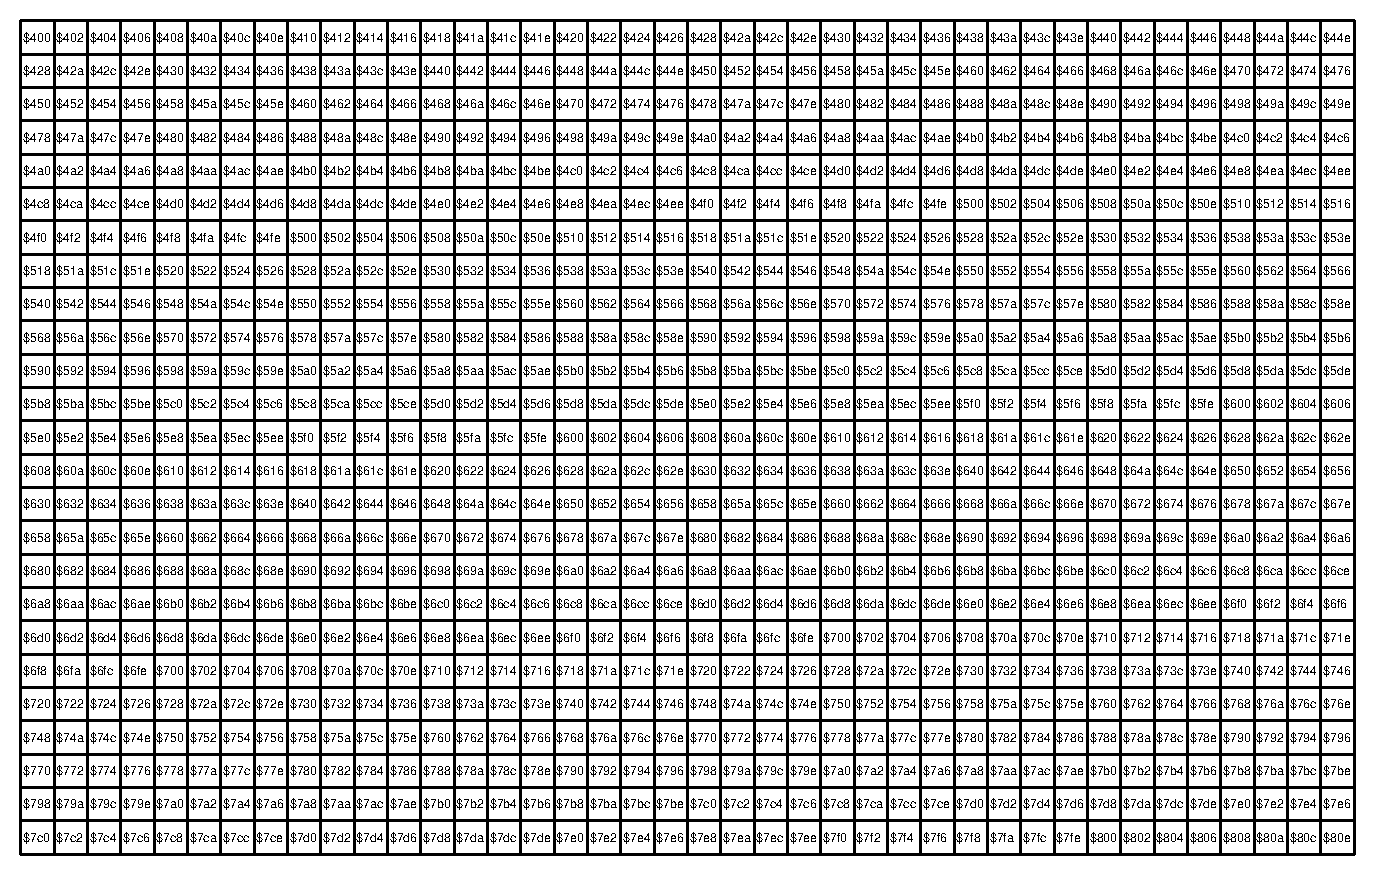
\includegraphics[width=\linewidth]{images/illustrations/screen-40x25-addresses16.pdf}

Er zijn twee zaken op te merken in de bovenstaande tabel: ten eerste vordert het adres met twee bytes per tekencel, omdat twee bytes nodig zijn om elk teken te definiëren. Ten tweede neemt het startadres van elke schermregel nog steeds slechts met 40 (\$28 in hexadecimaal) toe. Dit is niet wat we eigenlijk willen, want het betekent dat de eerste helft van de vorige regel opnieuw wordt weergegeven op elke huidige regel. Dit wordt opgelost door het aantal bytes dat per schermregel wordt overgeslagen in te stellen via \$D058 (LSB) en \$D059 (MSB). In dit geval willen we het aantal over te slaan bytes per regel te verhogen van 40 bytes naar 80 bytes. Dit kan door \$D058 in te stellen op 80 (\$50 in hexadecimaal) en \$D059 op 0. Dit geeft een scherminrichting als volgt:

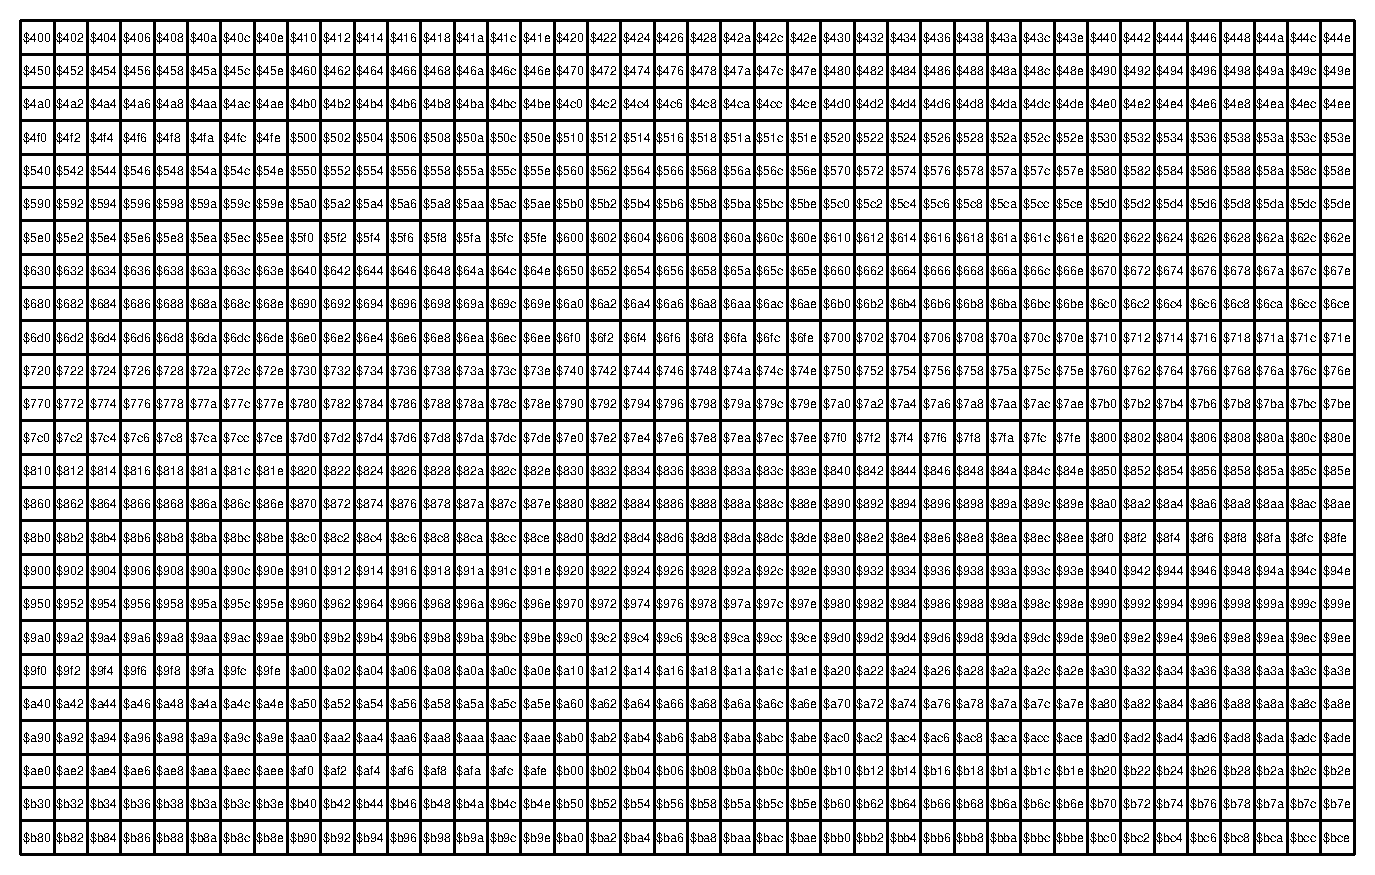
\includegraphics[width=\linewidth]{images/illustrations/screen-40x25-addresses16-80.pdf}

Het is mogelijk om Super-Uitgebreide Attribuutmodus te gebruiken vanuit C65-modus, door het scherm op 80 kolommen in te stellen, omdat de C65-ROM 2 KB reserveert voor zowel het schermgeheugen als het kleurengeheugen, en automatisch \$D058 en \$D059 op de juiste waarde zet voor 40$\times$2 = 80 bytes per schermregel. De gebruiker hoeft elk tekenpaar slechts als één Super-Uitgebreid Attribuutteken te behandelen en Super-Uitgebreide Attribuutmodus in te schakelen, zoals hierboven beschreven.

Omdat er paren van kleurengeheugen- en schermgeheugenbytes worden gebruikt om elk teken te definiëren, moet voorzichtig te werk worden gegaan bij het initialiseren en bewerken van het scherm. Een goede aanpak is om de tekstkleur op zwart in te stellen (kleurcode 0) en vervolgens het scherm te vullen met @-tekens, omdat dat tekencode 0 is. Vervolgens zijn er verschillende manieren om het scherm te bewerken. U kunt het normale PRINT-commando gebruiken en zorgvuldig tekenreeksen samenstellen die de juiste waarden in elk scherm- en kleurenbytepaar schrijven. Een andere aanpak is om de BANK- en POKE-commando's te gebruiken om de inhoud van het schermgeheugen en kleurengeheugen direct te instellen.

Het beheren van een scherm in Super-Uitgebreide Attribuutmodus op deze manier met BASIC 65 is natuurlijk eerder een noodoplossing en wordt alleen voorgesteld als een relatief eenvoudige manier om te beginnen met experimenteren. U wilt bijna zeker snel overschakelen op aangepaste schermverwerkingscode, het liefst in assembleertaal, om schermen in Super-Uitgebreide Attribuutmodus te bewerken. De aanpak met BASIC 65 kan echter behoorlijk krachtig zijn, omdat het bestaande scrollen van het scherm en andere bewerkingen beschikbaar blijven.

XXX Voorbeeldprogramma

De volgende beschrijvingen gaan ervan uit dat u een van de hierboven beschreven methoden heeft geïmplementeerd om het schermgeheugen en kleurengeheugen in te stellen.

\subsection{Volkleur-tekstmodus (256 kleuren per teken) (FCM)}

In de normale VIC-II/III-tekstmodus wordt één byte gebruikt voor elke pixelrij in een teken. Ter herinnering aan de werking van die modes: in hoge-resolutiemodus is elke pixel ofwel de achtergrond- ofwel de voorgrondkleur, gebaseerd op één bit in de byte. Kleurenmodus gebruikt twee bits om tussen vier mogelijke kleuren te kiezen, maar omdat er nog steeds slechts 8 bits beschikbaar zijn om elke rij van 8 pixels te beschrijven, heeft elk pixelpaar dezelfde kleur. De volkleur-tekstmodus van de VIC-IV schaft deze beperkingen op en maakt het mogelijk om elke pixel van een teken te kiezen uit 256 kleuren van de primaire of alternatieve paletbank, zonder horizontale resolutie op te offeren.

Hiertoe heeft elk teken nu 64 bytes aan gegevens nodig. Het adres van de gegevens is 64 $\times$ het tekennummer, ongeacht het adres van de tekenset. FCM hoort normaal gesproken te worden gebruikt met Super-Uitgebreide Attribuutmodus (SEAM), zodat meer dan 256 unieke tekens kunnen worden aangesproken. Omdat SEAM de keuze van 8.192 unieke tekens mogelijk maakt, kunnen FCM-tekengegevens overal in de eerste 512 KB chip-RAM worden geplaatst (let er echter op dat de meeste MEGA65-modellen slechts 384 KB chip-RAM hebben).

Let erop dat pixelwaarde \$ff niet direct de bijbehorende kleurcode selecteert. In plaats daarvan selecteert deze de kleurcode die is gedefinieerd door het kleurengeheugen.

\subsection{Nibble-kleuren-tekstmodus (16 kleuren per teken) (NCM)}

De Nibble-kleuren-modus (NCM) voor tekst lijkt op Volkleur-tekstmodus, met als verschil dat elke byte gegevens twee pixels beschrijft met elk 4 bits. Dit maakt NCM uniek, omdat de tekens 16 pixels breed zullen zijn in plaats van de gebruikelijke 8 pixels. Dit kan worden gebruikt om kleurrijke weergaven te maken, zonder zoveel geheugen te gebruiken als FCM, omdat er minder tekens nodig zijn om het scherm te bedekken. In tegenstelling tot de multicolourmodus (MCM) van de VIC-II heeft deze modus geen verlies van horizontale resolutie tot gevolg.

Bij NCM komen de onderste vier bits van de pixelkleur van de bovenste of onderste vier bits van de pixelgegevens. De bovenste vier bits van de kleurcode komen van de kleurengeheugengegevens van het weergegeven teken. Hierdoor is het mogelijk om alle paletingangen in NCM te gebruiken, hoewel de beperking van 16 kleuren per teken blijft bestaan. Vergelijkbaar met het gedrag van FCM selecteert pixelgegevenswaarde \$f de pixelkleur die is ingesteld in het kleurengeheugen.

Een verder voordeel van NCM is dat het minder buscycli per pixel gebruikt dan FCM, omdat er minder tekengegevens-ophaalbewerkingen per rasterlijn hoeven plaats te vinden. Samen met de verminderde geheugenbehoeften maakt dit NCM bijzonder geschikt voor het maken van kleurrijke grafische lagen. Hiermee kan de VIC-IV arcade-achtige weergaven met meer kleuren tonen dan bij veel 16-bits computers.


XXX

\subsection{Alphablending / Anti-aliasing}

De VIC-IV ondersteunt het mengen van tekens met de achtergrondkleur, waardoor effecten zoals anti-aliased lettertype-weergave mogelijk zijn. Het mengen is mogelijk op per-teken-basis. Het wordt ingeschakeld voor een specifiek teken als aan de volgende voorwaarden wordt voldaan:
\begin{enumerate}
  \item Het {\em ALPHAEN}-signaal is ingesteld in bit 7 van \$D054.  \item Het {\em CHR16}-signaal is ingesteld in bit 0 van \$D054 om Super-Uitgebreide Attribuutmodus (SEAM) in te schakelen.  \item Volkleur-tekstmodus (FCM) is ingeschakeld voor het teken.
\end{enumerate}
Indien alphablending is ingeschakeld voor een teken, worden de 8-bit pixelwaarden behandeld als alphawaarden in plaats van paletindices. De werkelijke pixelkleur wordt bepaald door de achtergrondkleur te mengen met de voorgrondkleur van het teken zoals gedefinieerd in het kleurengeheugen. Een alphawaarde van 0 staat voor volledige transparantie, waarbij alleen de achtergrondkleur van die pixel wordt weergegeven.

Merk op dat de alphablending alleen wordt toegepast tussen de achtergrondkleur en de voorgrondkleur van het teken. Dit betekent dat tekens achter het huidige teken feitelijk niet zichtbaar zullen zijn (tekenlagen kunnen worden samengesteld via GOTOX-herpositionering). Programmeurs moeten er echter van uitgaan dat het mengen met eerdere lagen in een toekomstige implementatie zal worden ondersteund. Om problemen met een dergelijke wijziging te voorkomen, plaatst u geen tekens achter een teken waarvoor alphablending is ingeschakeld.



\subsection{Tekens omdraaien}

XXX

\subsection{Variabele-breedte lettertypen}

Er zijn 4 bits waarmee pixels van de rechterrand van tekens kunnen worden weggesneden wanneer deze worden weergegeven. Dit heeft het effect dat tekens smaller worden. Dit kan nuttig zijn voor aantrekkelijkere tekstweergave, waarbij smallere tekens zoals ``i'' minder ruimte innemen dan bredere tekens zoals ``m'', zonder dat een bitmapdisplay nodig is. Deze functie kan worden gebruikt om variabele-breedte tekstweergave zeer efficiënt te maken, zowel wat betreft geheugengebruik als verwerkingstijd.

Deze functie kan worden gecombineerd met de volkleur-tekstmodus, de alfa-blendmodus en de 4-bits-per-pixel-modus om tekens mogelijk te maken met 15 intensiteitsniveaus tussen de achtergrond- en voorgrondkleur, en tot 16 pixels breed. Bovendien kan het GOTO-bit worden gebruikt om negatieve kerning toe te passen, zodat tekenparen zoals A en T geen overbodige witruimte tussen zich hebben wanneer ze naast elkaar worden afgedrukt. Het zorgvuldig gebruik van deze functies kan leiden tot indrukwekkende tekstweergave, vergelijkbaar met die op moderne 32-bits en 64-bits systemen, maar die nog steeds efficiënt genoeg is om te worden geïmplementeerd op een relatief beperkt systeem zoals de MEGA65. De presentatiesoftware ``MegaWAT!?’’'' voor de MEGA65 maakt gebruik van verschillende van deze functies om zijn aantrekkelijke, antialiased proportionele tekstweergave op dia's te produceren.

XXX MEGAWat!?!-screenshot

XXX Voorbeeldprogramma

\subsection{Raster Re-write Buffer}

Als het GOTO-bit is gezet voor een teken in Super-Uitgebreide Attribuutmodus, wordt in plaats van het teken te tekenen de positie op de rasterlijn teruggedraaid (of vooruitgeschoven) naar de pixelpositie die is opgegeven in de onderste 10 bits van de schermgeheugenbytes. Als het vertical flip-bit is gezet, heeft dit de alternatieve betekenis dat de achtergrondkleur niet wordt getekend. Deze combinatie kan worden gebruikt om tekstmateriaal over ander tekstmateriaal te plaatsen, wat een grove aanvulling vormt op de 8 hardware-sprites. De hoeveelheid materiaal is alleen beperkt door de rastertijd van de VIC-IV. Enige experimentatie is vereist om te bepalen hoeveel er in PAL- en NTSC-modus kan worden bereikt.

Als het GOTO-bit is gezet voor een teken en de tekenbreedte-verminderingsbits ook zijn gezet, worden deze geïnterpreteerd als een Y-offset die wordt opgeteld bij het tekengeheugenadres, maar alleen in Volkleurmodus. Instellen van Y=1 zorgt ervoor dat de tekendata worden opgehaald van 8 bytes verder, d.w.z. de eerste rij tekendata komt van het adres waar normaal de tweede rij tekendata zou worden opgehaald. Voor hogere waarden worden de tekendata opgehaald van verderop in de tekens. Door tekens zorgvuldig in het geheugen te rangschikken, kan deze functie worden gebruikt om vrije verticale positionering van soft sprites mogelijk te maken, zonder dat de tekendata hoeven te worden gekopieerd.

Als het GOTO-bit is gezet voor een teken en het Nybl Colour Mode (NCM)-bit ook is gezet, wordt het tweede kleurengeheugenbyte voor dat teken gebruikt om de \index{Rijmasker}rijmasker-bits in te stellen. Voor elk bit dat in het rijmasker is gezet, wordt de overeenkomstige rij tekens in de regel niet weergegeven. Dit kan worden gecombineerd met de Y-offsetfunctie om effectief een soepele verticale schuifregeling per teken mogelijk te maken.

De mogelijkheid om meerdere lagen tekst en grafisch materiaal te tekenen is zeer krachtig. Dit kan bijvoorbeeld worden gebruikt om meerdere overlappende lagen van apart schuifbare grafische elementen te bieden. Dit geeft veel van de voordelen van bitplane-gebaseerde playfields op andere computers, zoals de Amiga, maar zonder de nadelen van bitplanes.

Een goede introductie van de Raster Re-write Buffer en het gebruik ervan is te vinden in deze video:

\url{https://www.youtube.com/watch?v=00bm5uBeBos&feature=youtu.be}

Een belangrijk aspect van de RRB is dat de VIC-IV alleen de tekendata weergeeft die zich links van, en inclusief, het laatst getekende teken bevindt. Dit betekent dat wanneer u de GOTO-token gebruikt om meerdere lagen grafisch materiaal te overschrijven, u ofwel moet zorgen dat de laatste laag tot aan de rechterrand van het scherm reikt, ofwel een GOTO-token moet toevoegen dat de renderpositie naar de rechterrand van het scherm verplaatst.


XXX Voorbeeldprogramma

\section{Sprites}

\subsection{VIC-II/III-spritebesturing}

De besturing van sprites voor C64 / VIC-II/III-compatibiliteit is ongewijzigd ten opzichte van de C64. De enige praktische verschillen zijn zeer gering. In het bijzonder gebruikt de VIC-IV een ringbuffer voor de gegevens van elke sprite bij het renderen van een rasterlijn. Dit betekent dat een sprite meerdere keren per rasterlijn kan worden weergegeven, wat horizontale multiplexing mogelijk maakt.

\subsection{Uitgebreide sprite-afbeeldingssets}

Op de VIC-II en VIC-III moeten alle sprites hun afbeeldingsdata op een bepaald moment uit één enkel 16KB-geheugengebied halen. Dit beperkt het aantal verschillende sprite-afbeeldingen tot 256, omdat elke sprite-afbeelding 64 bytes in beslag neemt. In de praktijk moet hetzelfde 16KB-geheugengebied ook bitmap-, tekst- of bitplanedata bevatten, wat het aantal sprite-afbeeldingen dat tegelijk kan worden gebruikt aanzienlijk beperkt.

De VIC-IV heft deze beperking op doordat spritedata overal in het geheugen kunnen worden geplaatst, zij het nog steeds op 64-byte-grenzen. Dit wordt gedaan door het SPRPTR16-signaal in te stellen (bit 7, \$D06E, decimaal 53358), wat de VIC-IV vertelt dat er twee bytes per spritepointer in plaats van één moeten worden verwacht. Deze adressen zijn dan absolute adressen en negeren de 16KB VIC-II-bankselectielogica. Er zijn dus 16 bytes nodig in plaats van 8 bytes. De lijst met pointers kan ook overal in het geheugen worden geplaatst door de SPRPTRADR (\$D06C -- \$D06D, 53356 -- 53357 decimaal) en SPRPTRBNK-signalen (bits 0 -- 6, \$D06E, 53358 decimaal) in te stellen. Hierdoor kunnen spritedata overal in de eerste 4MB RAM worden geplaatst en de spritepointerlijst overal in de eerste 8MB RAM. Let op dat typische installaties van de VIC-IV slechts 384KB aangesloten RAM hebben, zodat deze beperkingen geen praktisch effect hebben. De bovenste bits van het SPRPTRBNK-signaal moeten echter op nul worden gezet om problemen met voorwaartse compatibiliteit te voorkomen.

Een reden voor ondersteuning van meer sprite-afbeeldingen is dat sprites op de VIC-IV meer dan één 64-byte-afbeeldingsslot kunnen vereisen. Het inschakelen van de modus voor extra-brede sprites betekent bijvoorbeeld dat een sprite 8$\times$21 = 168 bytes nodig heeft en dus vier VIC-II-stijl 64-byte-spriteafbeeldingsslots inneemt. Wanneer sprites met variabele hoogte worden gebruikt, kan dit oplopen tot 8$\times$255 = 2.040 bytes per sprite.

\subsection{Variabele spritegrootte}

Sprites kunnen met de VIC-IV een van drie breedtes hebben:

\begin{enumerate}
\item Normale VIC-II-breedte (24 pixels breed).\item Extra Breed, waarbij 64 bits (8 bytes) data per rasterlijn worden gebruikt in plaats van de 24 van de VIC-II. Dit resulteert in sprites die 64 pixels breed zijn, tenzij Volkleur-spritemodus is geselecteerd voor een sprite, in welk geval de sprite 64 bits $\div$ 4 bits per pixel = 16 pixels breed zal zijn.\item Tegelmodus, waarbij de sprite wordt herhaald getekend tot het einde van de rasterlijn. \\  Tegelmodus moet normaal gesproken alleen worden gebruikt met extra-brede sprites, omdat het tegelen altijd plaatsvindt met 64 bits spritedata per regel. Het inschakelen van tegelmodus met normale 24 bits brede mono- of multicolour-spritedata tekent 2 en 2/3 rijen spritedata als één regel, zelfs als de sprite niet in extra-brede modus staat, wat tot verwarrende weergave leidt.
\end{enumerate}

Om een sprite 64 pixels breed te maken (of 16 pixels als Volkleur-spritemodus is ingeschakeld), zet u het overeenkomstige bit voor de sprite in het SPRX64EN-register op (\$D057, 53335 decimaal). Het inschakelen van Volkleurmodus voor een sprite schakelt impliciet de uitgebreide breedtemodus in en zorgt ervoor dat deze sprites 16 pixels breed zijn.

Op vergelijkbare wijze kunnen sprites diverse hoogtes hebben: sprites zijn ofwel 21 pixels hoog zoals bij de VIC-II, ofwel, als het overeenkomstige bit voor de sprite is ingeschakeld in het SPRHGTEN-signaal (\$D055, 53333 decimaal), heeft die sprite de hoogte in pixels die is ingesteld in het SPRHGT-register (\$D056, 53334 decimaal), van 0 tot 255. Let op dat alle sprites met SPRHGTEN ingeschakeld dezelfde hoogte delen. Een sprite kan altijd de onderkant van zijn afbeeldingsdata transparant laten.

Om tegelmodus in te schakelen voor een sprite, zet u het bijbehorende bit van SPRTILEN. Voor sprites 0 tot en met 3 zet u bits 4 tot en met 7 van \$D04D (53325 decimaal). Voor sprites 4 tot en met 7 zet u bits 4 tot en met 7 van \$D04F (55327 decimaal).

\subsection{Variabele sprite-resolutie}

Standaard hebben sprites dezelfde resolutie als op de VIC-II, oftewel elke sprite-pixel is twee fysieke pixels breed en hoog. Het is echter mogelijk om sprites de native resolutie te laten gebruiken, waarbij sprite-pixels één fysiek pixel breed en/of hoog zijn. Dit wordt bereikt door het relevante bit voor de sprite in het SPRENV400-register (\$D076, 53366 decimaal) te zetten, zodat de verticale resolutie per sprite wordt vergroot. De horizontale resolutie van alle sprites is ofwel de normale VIC-II-resolutie, of wanneer het SPR640-signaal is gezet (bit 4 van \$D054, 53332 decimaal), hebben sprites dezelfde horizontale resolutie als de fysieke pixels van het beeldscherm.

\subsection{Sprite-paletbank}

De VIC-IV heeft vier paletbanken, in vergelijking met de enkele paletbank van de VIC-III. De VIC-IV maakt het mogelijk om afzonderlijke paletbanken te selecteren voor bitmap-/tekstgraphics en voor sprites. Dit maakt het eenvoudig om zeer kleurrijke beeldschermen te creëren, waarbij sprites andere kleuren hebben dan de rest van het beeldscherm, of om paletanimatie te gebruiken voor interessante visuele effecten in sprites, zonder het palet dat door andere elementen van het beeldscherm wordt gebruikt te verstoren.

De sprite-paletbank wordt geselecteerd door het SPRPALSEL-signaal in bits 2 en 3 van het register \$D070 (53360 decimaal) te zetten. Het is mogelijk om deze op dezelfde bank als de bitmap-/tekstweergave in te stellen, of om een andere paletbank te selecteren. De selectie van de paletbank wordt onmiddellijk van kracht. Vergeet niet dat u, om een palet te kunnen wijzigen, het palet ook in het bereik van de paletbankregisters op \$D100 -- \$D3FF moet plaatsen door het MAPEDPAL-signaal in bits 6 en 7 van \$D070 te zetten.

\subsection{Vollekleuren-spritemodus}

Naast de monochrome en multicolour-modi ondersteunt de VIC-IV een nieuwe vollekleuren-spritemodus. In deze modus worden vier bits gebruikt om elke sprite-pixel te coderen. In tegenstelling tot de multicolour-modus, waarin paren van bits paren van pixels coderen, behouden de pixels in de vollekleurenmodus hun normale horizontale resolutie. De kleur nul wordt als transparant beschouwd. Indien u zwart wilt gebruiken in een vollekleurensprite, moet u de paletbank die voor sprites is geselecteerd zodanig configureren dat een van de 15 kleuren voor de betreffende sprite de kleur zwart codeert.

De vollekleuren-spritemodus kan per sprite worden geselecteerd door het bijbehorende bit in het SPR16EN-register (\$D06B, 53355 decimaal) te zetten.

Om de acht sprites elk 15 unieke kleuren te laten hebben, wordt de spritekleur weergegeven met behulp van de paletingang die overeenkomt met: $spritenummer \times 16 + nibblewaarde$, waarbij $spritenummer$ het nummer van de sprite is (van 0 tot en met 7) en $nibblewaarde$ de waarde is van het halfbyte dat de spritegegevens voor de pixel bevat. Indien bovendien de bitplane-modus voor deze sprite is ingeschakeld, wordt 128 opgeteld bij de kleurwaarde, waardoor het eenvoudig wordt om tussen twee kleurenschema's voor een gegeven sprite te schakelen door slechts één bit in het SPRBPMEN-register te wijzigen.

Omdat de vollekleuren-spritemodus vier bits per pixel vereist, zijn sprites slechts zes pixels breed, tenzij extra-breed voor een sprite is ingeschakeld, in welk geval de sprite 16 pixels breed is. Tegelmodus kan gecombineerd worden met de vollekleuren-spritemodus, en heeft dan tot gevolg dat de 16 vollekleuren-pixels van de sprite worden herhaald tot aan het einde van de rasterlijn.

Het volgende BASIC-programma tekent een vollekleurensprite in C64- of C65-modus:

\begin{screencode}
10 PRINT CHR$(147)
20 REM C65-/C64-MODUS DETECTEREN
30 IF PEEK(53272) AND 32 THEN GOTO 100
40 POKE 53295,ASC("G"):POKE 53295,ASC("S")
100 REM Sprite instellen
110 AD=4096                         :REM $1000-spriteadres
120 TC=10                           :REM transparante kleur
130 SPR=PEEK(53356)+PEEK(53357)*256 :REM sprite-tabeladres ophalen
140 POKE SPR,AD/64                  :REM spriteadres instellen
150 FOR I=AD TO AD+168              :REM sprite met TC wissen
160 POKE I,TC+TC*16                 :REM een byte = 2 pixels
170 NEXT
180 POKE 53287,TC                   :REM transparante kleur instellen
190 POKE 53248,100                  :REM sprite op 100,100 zetten...
200 POKE 53249,100                  :REM op het scherm op 100,100
210 POKE 53355,1                    :REM sprite 0 16-kleurig maken
220 POKE 53335,1                    :REM sprite 0 16X4-bits laten gebruiken
230 POKE 53269,1                    :REM sprite 0 inschakelen
240 GOSUB 900                       :REM meerkleurensprite lezen
250 END

900 REM Sprite uit gegevens laden
910 READ N$:IF N$="END" THEN RETURN
920 GOSUB 1000                      :REM regel decoderen
930 GOTO 910

\end{screencode}

\begin{screencode}
1000 REM Tekenreeks van nibbles in N$ op adres AD decoderen
1010 IF LEN(N$)<>16 THEN PRINT "ILLEGAL SPR DATA!":END
1020 FOR I=1 TO 16 STEP 2
1030 N=(ASC(MID$(N$,I,1))-ASC("@"))    :REM hoge nibble
1040 IF N<0 THEN N=TC                  :REM . is transparant
1050 M=(ASC(MID$(N$,I+1,1))-ASC("@"))  :REM lage nibble
1060 IF M<0 THEN M=TC                  :REM . is transparant
1070 POKE AD,(N AND 15)*16 + (M AND 15):REM 2 pixels instellen
1080 AD=AD+1                           :REM AD ophogen
1090 NEXT I
1100 RETURN

1998 REM Spritegegevens
1999 REM . = transparant, @-O = kleuren 0 tot 15
2000 DATA "..AAFF...HHCC..."
2010 DATA ".AAFF.....HHCC.."
2020 DATA "AAFF.......HHCC."
2030 DATA "AFF...@@@...HHC."
2040 DATA "FF..@@GGG@@..HH."
2050 DATA "..@@GGGGGGG@@..."
2060 DATA ".@GGGGGGGGGGG@.."
2070 DATA ".@GGGGGGGGGGG@.."
2080 DATA "@GGG@@GGG@@GGG@."
2090 DATA "@GG@GGGGGGG@GG@."
2100 DATA "@GGGGGGGGGGGGG@."
2110 DATA "@GGGGGBGBGGGGG@."
2120 DATA "@GGGBBBBBBBGGG@."
2130 DATA ".@GGGGBBBGGGG@.."
2140 DATA ".@GGGGGBGGGGG@.."
2150 DATA "..@@GGGGGGG@@..."
2160 DATA "II..@@GGG@@..KK."
2170 DATA "DII...@@@...KKE."
2180 DATA "DDII.......KKEE."
2190 DATA ".DDII.....KKEE.."
2200 DATA "..DDII...KKEE..."
2210 DATA "END"
\end{screencode}
\clearpage

\section{VIC-III errata-niveau}

Er zijn een aantal gevallen waarin de VIC-III-chip in de bekende Commodore 65-prototypen niet overeenkomstig de specificatie functioneert, de specificatie onvoldoende detail bevat en de implementatie opmerkelijk inconsistent is, of het ontwerp zelf gebreken of inconsistenties vertoont. Het standaardgedrag van de VIC-IV is om de VIC-III in deze gevallen zo nauwkeurig mogelijk te emuleren. In sommige gevallen waarin het gedrag van de VIC-III tekortschiet, biedt de VIC-IV verbeterd gedrag, dat door software kan worden geselecteerd met behulp van het HWERRATA-register op \$D08F.

Omdat deze correcties achterwaarts onverenigbaar zijn met de VIC-III en met eerdere versies van de VIC-IV en de MEGA65-core, moet software deze correcties expliciet activeren door het HWERRATA-register te zetten. Dit beschermt software tegen verdere wijzigingen die in toekomstige versies van de MEGA65-core kunnen worden geïntroduceerd. De beginstand van dit register is \$00, wat volledige compatibiliteit met de VIC-III aanvraagt, inclusief het foutieve gedrag. De MEGA65-ROM zal dit register bij het starten van programma's altijd op \$00 laten staan. Een programma kan HWERRATA instellen om een set correcties te activeren die de ontwikkelaar bij het schrijven van het programma kende, en achterwaarts onverenigbare correcties uit te sluiten die in latere versies kunnen worden geïntroduceerd.

Het aanvragen van een errata-niveau activeert alle correcties tot dat niveau. Er is bewust geen mogelijkheid om een niveau aan te vragen en specifieke correcties op lagere niveaus uit te sluiten. U moet uw programma zodanig schrijven dat het alle correcties tot het gevraagde niveau ondersteunt.

In gevallen waarin het activeren van een correctie het gedrag van een heet register wijzigt, zal het instellen van het errata-niveau hete-registerpropagatie {\em{niet}} activeren. Het programma moet de hete-registerpropagatie zelf activeren door een 1 te schrijven naar het HOTREG-register.

De tot nu toe geïmplementeerde errata-niveaus zijn als volgt:

\subsubsection{VIC-III errata-niveaus}

\begin{longtable}{|p{1.5cm}|p{7.1cm}|p{2.5cm}|}
\hhline{---}
{\bf{Niveau}} & {\bf{Gecorrigeerd gedrag}} & {\bf{Ge\"introduceerd in}} \\
\hhline{---}
\endhead
\multicolumn{3}{l@{}}{vervolg \ldots}\\
\endfoot
\hline
\endlastfoot

{\bf{0}} & Geen correcties. Volledig VIC-III-compatibel. & N/A \\

\hline
{\bf{1}} & {\bf{X-scrollpositie verschoven in de H640-modus.}} De VIC-III geeft de X-scrollpositie voor het vloeiend scrollen van tekst (\$D016 XSCL) onjuist weer in de H640-modus. De correctie verschuift de scrollpositie met 1 logische pixel (2 fysieke pixels) naar rechts. Dit wordt pas van kracht na de hot register-propagatie. &v0.96 \\

\hline
{\bf{X}} & {\bf{Gedrag van de busy-vlag van de SD-kaart.}} De busy-vlag van de SD-kaart (bit 1 van \$D680) geeft aan of de SD-kaartcontroller op laag niveau bezig is. Door de toevoeging van de read-ahead-functionaliteit van de SD-kaartcontroller zal oudere software, die erop rekent dat dit bit vrijkomt na voltooiing van een leesbewerking, ten onrechte wachten totdat de volledige read-ahead-sequentie is afgerond. Dit kan er op zijn beurt toe leiden dat software ten onrechte meent dat het lezen van de sector is mislukt vanwege de langere benodigde tijd, of dat een ander leesverzoek niet onmiddellijk kan worden ingediend. Daarom geeft de busy-vlag van de SD-kaart onder dit errata-niveau niet aan of de SD-kaartcontroller een read-ahead-bewerking op de achtergrond voor een sector uitvoert. Op of boven dit errata-niveau wordt deze informatie niet verborgen: bit 0 komt vrij wanneer de gevraagde sector beschikbaar is, maar bit 1 blijft gezet zolang een read-ahead-bewerking doorgaat. &Nog niet geïmplementeerd \\

\end{longtable}


\section{VIC-II / C64-registers}

\setlength{\tabcolsep}{0pt}
\begin{longtable}{|C{12.5mm}|C{12.5mm}|C{12.5mm}|C{12.5mm}|C{12.5mm}|C{12.5mm}|C{12.5mm}|C{12.5mm}|C{12.5mm}|C{12.5mm}|}
\hline
{\bf{HEX}} & {\bf{DEC}} & {\bf{DB7}} & {\bf{DB6}} & {\bf{DB5}} & {\bf{DB4}} & {\bf{DB3}} & {\bf{DB2}} & {\bf{DB1}} & {\bf{DB0}} \\
\hline
\endfirsthead
\multicolumn{3}{l@{}}{\ldots vervolgd}\\
\hline
{\bf{HEX}} & {\bf{DEC}} & {\bf{DB7}} & {\bf{DB6}} & {\bf{DB5}} & {\bf{DB4}} & {\bf{DB3}} & {\bf{DB2}} & {\bf{DB1}} & {\bf{DB0}} \\
\endhead
\multicolumn{3}{l@{}}{vervolgd \ldots}\\
\endfoot
\hline
\endlastfoot
\footnotesize  D000\index{Registers!\$D000} \index{Registers!53248} & \footnotesize 53248 & \multicolumn{8}{c|}{\footnotesize S0X\index{Registers!SNX}}\\
\hline
\footnotesize  D001\index{Registers!\$D001} \index{Registers!53249} & \footnotesize 53249 & \multicolumn{8}{c|}{\footnotesize S0Y\index{Registers!SNY}}\\
\hline
\footnotesize  D002\index{Registers!\$D002} \index{Registers!53250} & \footnotesize 53250 & \multicolumn{8}{c|}{\footnotesize S1X\index{Registers!S1X}}\\
\hline
\footnotesize  D003\index{Registers!\$D003} \index{Registers!53251} & \footnotesize 53251 & \multicolumn{8}{c|}{\footnotesize S1Y\index{Registers!S1Y}}\\
\hline
\footnotesize  D004\index{Registers!\$D004} \index{Registers!53252} & \footnotesize 53252 & \multicolumn{8}{c|}{\footnotesize S2X\index{Registers!S2X}}\\
\hline
\footnotesize  D005\index{Registers!\$D005} \index{Registers!53253} & \footnotesize 53253 & \multicolumn{8}{c|}{\footnotesize S2Y\index{Registers!S2Y}}\\
\hline
\footnotesize  D006\index{Registers!\$D006} \index{Registers!53254} & \footnotesize 53254 & \multicolumn{8}{c|}{\footnotesize S3X\index{Registers!S3X}}\\
\hline
\footnotesize  D007\index{Registers!\$D007} \index{Registers!53255} & \footnotesize 53255 & \multicolumn{8}{c|}{\footnotesize S3Y\index{Registers!S3Y}}\\
\hline
\footnotesize  D008\index{Registers!\$D008} \index{Registers!53256} & \footnotesize 53256 & \multicolumn{8}{c|}{\footnotesize S4X\index{Registers!S4X}}\\
\hline
\footnotesize  D009\index{Registers!\$D009} \index{Registers!53257} & \footnotesize 53257 & \multicolumn{8}{c|}{\footnotesize S4Y\index{Registers!S4Y}}\\
\hline
\footnotesize  D00A\index{Registers!\$D00A} \index{Registers!53258} & \footnotesize 53258 & \multicolumn{8}{c|}{\footnotesize S5X\index{Registers!S5X}}\\
\hline
\footnotesize  D00B\index{Registers!\$D00B} \index{Registers!53259} & \footnotesize 53259 & \multicolumn{8}{c|}{\footnotesize S5Y\index{Registers!S5Y}}\\
\hline
\footnotesize  D00C\index{Registers!\$D00C} \index{Registers!53260} & \footnotesize 53260 & \multicolumn{8}{c|}{\footnotesize S6X\index{Registers!S6X}}\\
\hline
\footnotesize  D00D\index{Registers!\$D00D} \index{Registers!53261} & \footnotesize 53261 & \multicolumn{8}{c|}{\footnotesize S6Y\index{Registers!S6Y}}\\
\hline
\footnotesize  D00E\index{Registers!\$D00E} \index{Registers!53262} & \footnotesize 53262 & \multicolumn{8}{c|}{\footnotesize S7X\index{Registers!S7X}}\\
\hline
\footnotesize  D00F\index{Registers!\$D00F} \index{Registers!53263} & \footnotesize 53263 & \multicolumn{8}{c|}{\footnotesize S7Y\index{Registers!S7Y}}\\
\hline
\footnotesize  D010\index{Registers!\$D010} \index{Registers!53264} & \footnotesize 53264 & \multicolumn{8}{c|}{\footnotesize SXMSB\index{Registers!SXMSB}}\\
\hline
\footnotesize  D011\index{Registers!\$D011} \index{Registers!53265} & \footnotesize 53265 & \footnotesize RC8 & \footnotesize ECM & \footnotesize BMM & \footnotesize BLNK & \footnotesize RSEL & \multicolumn{3}{c|}{\footnotesize YSCL\index{Registers!YSCL}}\\
\hline
\footnotesize  D012\index{Registers!\$D012} \index{Registers!53266} & \footnotesize 53266 & \multicolumn{8}{c|}{\footnotesize RC\index{Registers!RC}}\\
\hline
\footnotesize  D013\index{Registers!\$D013} \index{Registers!53267} & \footnotesize 53267 & \multicolumn{8}{c|}{\footnotesize LPX\index{Registers!LPX}}\\
\hline
\footnotesize  D014\index{Registers!\$D014} \index{Registers!53268} & \footnotesize 53268 & \multicolumn{8}{c|}{\footnotesize LPY\index{Registers!LPY}}\\
\hline
\footnotesize  D015\index{Registers!\$D015} \index{Registers!53269} & \footnotesize 53269 & \multicolumn{8}{c|}{\footnotesize SE\index{Registers!SE}}\\
\hline
\footnotesize  D016\index{Registers!\$D016} \index{Registers!53270} & \footnotesize 53270 & \multicolumn{2}{c|}{\footnotesize --}& \footnotesize RST & \footnotesize MCM & \footnotesize CSEL & \multicolumn{3}{c|}{\footnotesize XSCL\index{Registers!XSCL}}\\
\hline
\footnotesize  D017\index{Registers!\$D017} \index{Registers!53271} & \footnotesize 53271 & \multicolumn{8}{c|}{\footnotesize SEXY\index{Registers!SEXY}}\\
\hline
\footnotesize  D018\index{Registers!\$D018} \index{Registers!53272} & \footnotesize 53272 & \multicolumn{4}{c|}{\footnotesize VS\index{Registers!VS}}& \multicolumn{3}{c|}{\footnotesize CB\index{Registers!CB}}& \footnotesize -- \\
\hline
\footnotesize  D019\index{Registers!\$D019} \index{Registers!53273} & \footnotesize 53273 & \multicolumn{4}{c|}{\footnotesize --}& \footnotesize ILP & \footnotesize ISSC & \footnotesize ISBC & \footnotesize RIRQ \\
\hline
\footnotesize  D01A\index{Registers!\$D01A} \index{Registers!53274} & \footnotesize 53274 & \multicolumn{5}{c|}{\footnotesize --}& \footnotesize MISSC & \footnotesize MISBC & \footnotesize MRIRQ \\
\hline
\footnotesize  D01B\index{Registers!\$D01B} \index{Registers!53275} & \footnotesize 53275 & \multicolumn{8}{c|}{\footnotesize BSP\index{Registers!BSP}}\\
\hline
\footnotesize  D01C\index{Registers!\$D01C} \index{Registers!53276} & \footnotesize 53276 & \multicolumn{8}{c|}{\footnotesize SCM\index{Registers!SCM}}\\
\hline
\footnotesize  D01D\index{Registers!\$D01D} \index{Registers!53277} & \footnotesize 53277 & \multicolumn{8}{c|}{\footnotesize SEXX\index{Registers!SEXX}}\\
\hline
\footnotesize  D01E\index{Registers!\$D01E} \index{Registers!53278} & \footnotesize 53278 & \multicolumn{8}{c|}{\footnotesize SSC\index{Registers!SSC}}\\
\hline
\footnotesize  D01F\index{Registers!\$D01F} \index{Registers!53279} & \footnotesize 53279 & \multicolumn{8}{c|}{\footnotesize SBC\index{Registers!SBC}}\\
\hline
\footnotesize  D020\index{Registers!\$D020} \index{Registers!53280} & \footnotesize 53280 & \multicolumn{4}{c|}{\footnotesize --}& \multicolumn{4}{c|}{\footnotesize BORDERCOL\index{Registers!BORDERCOL}}\\
\hline
\footnotesize  D021\index{Registers!\$D021} \index{Registers!53281} & \footnotesize 53281 & \multicolumn{4}{c|}{\footnotesize --}& \multicolumn{4}{c|}{\footnotesize SCREENCOL\index{Registers!SCREENCOL}}\\
\hline
\footnotesize  D022\index{Registers!\$D022} \index{Registers!53282} & \footnotesize 53282 & \multicolumn{4}{c|}{\footnotesize --}& \multicolumn{4}{c|}{\footnotesize MC1\index{Registers!MC1}}\\
\hline
\footnotesize  D023\index{Registers!\$D023} \index{Registers!53283} & \footnotesize 53283 & \multicolumn{4}{c|}{\footnotesize --}& \multicolumn{4}{c|}{\footnotesize MC2\index{Registers!MC2}}\\
\hline
\footnotesize  D024\index{Registers!\$D024} \index{Registers!53284} & \footnotesize 53284 & \multicolumn{4}{c|}{\footnotesize --}& \multicolumn{4}{c|}{\footnotesize MC3\index{Registers!MC3}}\\
\hline
\footnotesize  D025\index{Registers!\$D025} \index{Registers!53285} & \footnotesize 53285 & \multicolumn{8}{c|}{\footnotesize SPRMC0\index{Registers!SPRMC0}}\\
\hline
\footnotesize  D026\index{Registers!\$D026} \index{Registers!53286} & \footnotesize 53286 & \multicolumn{8}{c|}{\footnotesize SPRMC1\index{Registers!SPRMC1}}\\
\hline
\footnotesize  D027\index{Registers!\$D027} \index{Registers!53287} & \footnotesize 53287 & \multicolumn{8}{c|}{\footnotesize SPR0COL\index{Registers!SPRNCOL}}\\
\hline
\footnotesize  D028\index{Registers!\$D028} \index{Registers!53288} & \footnotesize 53288 & \multicolumn{8}{c|}{\footnotesize SPR1COL\index{Registers!SPR1COL}}\\
\hline
\footnotesize  D029\index{Registers!\$D029} \index{Registers!53289} & \footnotesize 53289 & \multicolumn{8}{c|}{\footnotesize SPR2COL\index{Registers!SPR2COL}}\\
\hline
\footnotesize  D02A\index{Registers!\$D02A} \index{Registers!53290} & \footnotesize 53290 & \multicolumn{8}{c|}{\footnotesize SPR3COL\index{Registers!SPR3COL}}\\
\hline
\footnotesize  D02B\index{Registers!\$D02B} \index{Registers!53291} & \footnotesize 53291 & \multicolumn{8}{c|}{\footnotesize SPR4COL\index{Registers!SPR4COL}}\\
\hline
\footnotesize  D02C\index{Registers!\$D02C} \index{Registers!53292} & \footnotesize 53292 & \multicolumn{8}{c|}{\footnotesize SPR5COL\index{Registers!SPR5COL}}\\
\hline
\footnotesize  D02D\index{Registers!\$D02D} \index{Registers!53293} & \footnotesize 53293 & \multicolumn{8}{c|}{\footnotesize SPR6COL\index{Registers!SPR6COL}}\\
\hline
\footnotesize  D02E\index{Registers!\$D02E} \index{Registers!53294} & \footnotesize 53294 & \multicolumn{8}{c|}{\footnotesize SPR7COL\index{Registers!SPR7COL}}\\
\hline
\footnotesize  D02F\index{Registers!\$D02F} \index{Registers!53295} & \footnotesize 53295 & \multicolumn{8}{c|}{\footnotesize KEY\index{Registers!KEY}}\\
\hline
\footnotesize  D030\index{Registers!\$D030} \index{Registers!53296} & \footnotesize 53296 & \multicolumn{7}{c|}{\footnotesize --}& \footnotesize C128\-FAST \\
\hline
\end{longtable}
\begin{itemize}
\item{\bf{BLNK}\index{Registers!BLNK}} Weergave inschakelen: 0 = weergave uitschakelen, 1 = weergave inschakelen
\item{\bf{BMM}\index{Registers!BMM}} Bitmapmodus
\item{\bf{BORDERCOL}\index{Registers!BORDERCOL}} Randkleur van het scherm (16 kleuren)
\item{\bf{BSP}\index{Registers!BSP}} Bitstelling sprite-/achtergrondprioriteit
\item{\bf{C128FAST}\index{Registers!C128FAST}} 2 MHz-selectie (voor C128 2 MHz-emulatie)
\item{\bf{CB}\index{Registers!CB}} Adreslocatie van de tekenset (× 1 KiB)
\item{\bf{CSEL}\index{Registers!CSEL}} 38/40-kolommenselectie
\item{\bf{ECM}\index{Registers!ECM}} Uitgebreide achtergrondmodus
\item{\bf{ILP}\index{Registers!ILP}} Lichtpen indicator of bevestiging
\item{\bf{ISBC}\index{Registers!ISBC}} Sprite-/bitmapbotsing indicator of bevestiging
\item{\bf{ISSC}\index{Registers!ISSC}} Sprite-/spritebotsing indicator of bevestiging
\item{\bf{KEY}\index{Registers!KEY}} \$00 en dan \$00 schrijven om C64/VIC-II I/O-registers in te schakelen
\item{\bf{LPX}\index{Registers!LPX}} Grove horizontale bundelpositie (was lichtpen X)
\item{\bf{LPY}\index{Registers!LPY}} Grove verticale bundelpositie (was lichtpen Y)
\item{\bf{MC1}\index{Registers!MC1}} Multikleur 1 (16 kleuren)
\item{\bf{MC2}\index{Registers!MC2}} Multikleur 2 (16 kleuren)
\item{\bf{MC3}\index{Registers!MC3}} Multikleur 3 (16 kleuren)
\item{\bf{MCM}\index{Registers!MCM}} Multikleurmodus
\item{\bf{MISBC}\index{Registers!MISBC}} Masker sprite-/bitmapbotsing IRQ
\item{\bf{MISSC}\index{Registers!MISSC}} Masker sprite-/spritebotsing IRQ
\item{\bf{MRIRQ}\index{Registers!MRIRQ}} Masker rasterIRQ
\item{\bf{RC}\index{Registers!RC}} Rastervergelijking bits 0 tot 7
\item{\bf{RC8}\index{Registers!RC8}} Rastervergelijking bit 8
\item{\bf{RIRQ}\index{Registers!RIRQ}} Rastervergelijking indicator of bevestiging
\item{\bf{RSEL}\index{Registers!RSEL}} 24/25-rijselectie
\item{\bf{RST}\index{Registers!RST}} Schakelt de video-uitvoer op de MAX Machine(tm) VIC-II 6566 uit. Wordt genegeerd op normale C64-computers en de MEGA65
\item{\bf{SBC}\index{Registers!SBC}} Indicatiebits voor sprite/voorgrondbotsing
\item{\bf{SCM}\index{Registers!SCM}} Inschakelbits voor de sprite-multikleur
\item{\bf{SCREENCOL}\index{Registers!SCREENCOL}} Schermkleur (16 kleuren)
\item{\bf{SE}\index{Registers!SE}} Inschakelbits voor sprites
\item{\bf{SEXX}\index{Registers!SEXX}} Inschakelbits voor horizontale sprite-vergroting
\item{\bf{SEXY}\index{Registers!SEXY}} Inschakelbits voor verticale sprite-vergroting
\item{\bf{SNX}\index{Registers!SNX}} Horizontale positie van sprite N
\item{\bf{SNY}\index{Registers!SNY}} Verticale positie van sprite N
\item{\bf{SPRMC0}\index{Registers!SPRMC0}} Sprite-multikleur 0
\item{\bf{SPRMC1}\index{Registers!SPRMC1}} Sprite-multikleur 1
\item{\bf{SPRNCOL}\index{Registers!SPRNCOL}} Kleur van sprite N / transparantiekleur van de sprite in 16-kleurenmodus (lagere nibble)
\item{\bf{SSC}\index{Registers!SSC}} Indicatiebits voor sprite/spritebotsing
\item{\bf{SXMSB}\index{Registers!SXMSB}} MSB's van de horizontale sprite-positie
\item{\bf{VS}\index{Registers!VS}} Schermadres ($\times$ 1KiB)
\item{\bf{XSCL}\index{Registers!XSCL}} Horizontaal vloeiend scrollen
\item{\bf{YSCL}\index{Registers!YSCL}} 24/25 verticaal vloeiend scrollen
\end{itemize}


\section{VIC-III / C65-registers}

\setlength{\tabcolsep}{0pt}
\begin{longtable}{|C{12.5mm}|C{12.5mm}|C{12.5mm}|C{12.5mm}|C{12.5mm}|C{12.5mm}|C{12.5mm}|C{12.5mm}|C{12.5mm}|C{12.5mm}|}
\hline
{\bf{HEX}} & {\bf{DEC}} & {\bf{DB7}} & {\bf{DB6}} & {\bf{DB5}} & {\bf{DB4}} & {\bf{DB3}} & {\bf{DB2}} & {\bf{DB1}} & {\bf{DB0}} \\
\hline
\endfirsthead
\multicolumn{3}{l@{}}{\ldots vervolgd}\\
\hline
{\bf{HEX}} & {\bf{DEC}} & {\bf{DB7}} & {\bf{DB6}} & {\bf{DB5}} & {\bf{DB4}} & {\bf{DB3}} & {\bf{DB2}} & {\bf{DB1}} & {\bf{DB0}} \\
\endhead
\multicolumn{3}{l@{}}{vervolgd \ldots}\\
\endfoot
\hline
\endlastfoot
\footnotesize  D020\index{Registers!\$D020} \index{Registers!53280} & \footnotesize 53280 & \multicolumn{8}{c|}{\footnotesize BORDERCOL\index{Registers!BORDERCOL}}\\
\hline
\footnotesize  D021\index{Registers!\$D021} \index{Registers!53281} & \footnotesize 53281 & \multicolumn{8}{c|}{\footnotesize SCREENCOL\index{Registers!SCREENCOL}}\\
\hline
\footnotesize  D022\index{Registers!\$D022} \index{Registers!53282} & \footnotesize 53282 & \multicolumn{8}{c|}{\footnotesize MC1\index{Registers!MC1}}\\
\hline
\footnotesize  D023\index{Registers!\$D023} \index{Registers!53283} & \footnotesize 53283 & \multicolumn{8}{c|}{\footnotesize MC2\index{Registers!MC2}}\\
\hline
\footnotesize  D024\index{Registers!\$D024} \index{Registers!53284} & \footnotesize 53284 & \multicolumn{8}{c|}{\footnotesize MC3\index{Registers!MC3}}\\
\hline
\footnotesize  D025\index{Registers!\$D025} \index{Registers!53285} & \footnotesize 53285 & \multicolumn{8}{c|}{\footnotesize SPRMC0\index{Registers!SPRMC0}}\\
\hline
\footnotesize  D026\index{Registers!\$D026} \index{Registers!53286} & \footnotesize 53286 & \multicolumn{8}{c|}{\footnotesize SPRMC1\index{Registers!SPRMC1}}\\
\hline
\footnotesize  D02F\index{Registers!\$D02F} \index{Registers!53295} & \footnotesize 53295 & \multicolumn{8}{c|}{\footnotesize KEY\index{Registers!KEY}}\\
\hline
\footnotesize  D030\index{Registers!\$D030} \index{Registers!53296} & \footnotesize 53296 & \footnotesize ROME & \footnotesize CROM9 & \footnotesize ROMC & \footnotesize ROMA & \footnotesize ROM8 & \footnotesize PAL & \footnotesize EXTSYNC & \footnotesize CRAM2K \\
\hline
\footnotesize  D031\index{Registers!\$D031} \index{Registers!53297} & \footnotesize 53297 & \footnotesize H640 & \footnotesize FAST & \footnotesize ATTR & \footnotesize BPM & \footnotesize V400 & \footnotesize H1280 & \footnotesize MONO & \footnotesize INT \\
\hline
\footnotesize  D032\index{Registers!\$D032} \index{Registers!53298} & \footnotesize 53298 & \multicolumn{8}{c|}{\footnotesize BPENABLE\index{Registers!BPENABLE}}\\
\hline
\footnotesize  D033\index{Registers!\$D033} \index{Registers!53299} & \footnotesize 53299 & \multicolumn{3}{c|}{\footnotesize B0ADODD\index{Registers!BXADODD}}& \footnotesize -- & \multicolumn{3}{c|}{\footnotesize B0ADEVN\index{Registers!BXADEVN}}& \footnotesize -- \\
\hline
\footnotesize  D034\index{Registers!\$D034} \index{Registers!53300} & \footnotesize 53300 & \multicolumn{3}{c|}{\footnotesize B1ADODD\index{Registers!BYADODD}}& \footnotesize -- & \multicolumn{3}{c|}{\footnotesize B1ADEVN\index{Registers!BYADEVN}}& \footnotesize -- \\
\hline
\footnotesize  D035\index{Registers!\$D035} \index{Registers!53301} & \footnotesize 53301 & \multicolumn{3}{c|}{\footnotesize B2ADODD\index{Registers!B2ADODD}}& \footnotesize -- & \multicolumn{3}{c|}{\footnotesize B2ADEVN\index{Registers!B2ADEVN}}& \footnotesize -- \\
\hline
\footnotesize  D036\index{Registers!\$D036} \index{Registers!53302} & \footnotesize 53302 & \multicolumn{3}{c|}{\footnotesize B3ADODD\index{Registers!B3ADODD}}& \footnotesize -- & \multicolumn{3}{c|}{\footnotesize B3ADEVN\index{Registers!B3ADEVN}}& \footnotesize -- \\
\hline
\footnotesize  D037\index{Registers!\$D037} \index{Registers!53303} & \footnotesize 53303 & \multicolumn{3}{c|}{\footnotesize B4ADODD\index{Registers!B4ADODD}}& \footnotesize -- & \multicolumn{3}{c|}{\footnotesize B4ADEVN\index{Registers!B4ADEVN}}& \footnotesize -- \\
\hline
\footnotesize  D038\index{Registers!\$D038} \index{Registers!53304} & \footnotesize 53304 & \multicolumn{3}{c|}{\footnotesize B5ADODD\index{Registers!B5ADODD}}& \footnotesize -- & \multicolumn{3}{c|}{\footnotesize B5ADEVN\index{Registers!B5ADEVN}}& \footnotesize -- \\
\hline
\footnotesize  D039\index{Registers!\$D039} \index{Registers!53305} & \footnotesize 53305 & \multicolumn{3}{c|}{\footnotesize B6ADODD\index{Registers!B6ADODD}}& \footnotesize -- & \multicolumn{3}{c|}{\footnotesize B6ADEVN\index{Registers!B6ADEVN}}& \footnotesize -- \\
\hline
\footnotesize  D03A\index{Registers!\$D03A} \index{Registers!53306} & \footnotesize 53306 & \multicolumn{3}{c|}{\footnotesize B7ADODD\index{Registers!B7ADODD}}& \footnotesize -- & \multicolumn{3}{c|}{\footnotesize B7ADEVN\index{Registers!B7ADEVN}}& \footnotesize -- \\
\hline
\footnotesize  D03B\index{Registers!\$D03B} \index{Registers!53307} & \footnotesize 53307 & \multicolumn{8}{c|}{\footnotesize BPCOMP\index{Registers!BPCOMP}}\\
\hline
\footnotesize  D03C\index{Registers!\$D03C} \index{Registers!53308} & \footnotesize 53308 & \multicolumn{8}{c|}{\footnotesize BPX\index{Registers!BPX}}\\
\hline
\footnotesize  D03D\index{Registers!\$D03D} \index{Registers!53309} & \footnotesize 53309 & \multicolumn{8}{c|}{\footnotesize BPY\index{Registers!BPY}}\\
\hline
\footnotesize  D03E\index{Registers!\$D03E} \index{Registers!53310} & \footnotesize 53310 & \multicolumn{8}{c|}{\footnotesize HPOS\index{Registers!HPOS}}\\
\hline
\footnotesize  D03F\index{Registers!\$D03F} \index{Registers!53311} & \footnotesize 53311 & \multicolumn{8}{c|}{\footnotesize VPOS\index{Registers!VPOS}}\\
\hline
\footnotesize  D040\index{Registers!\$D040} \index{Registers!53312} & \footnotesize 53312 & \multicolumn{8}{c|}{\footnotesize B0PIX\index{Registers!BNPIX}}\\
\hline
\footnotesize  D041\index{Registers!\$D041} \index{Registers!53313} & \footnotesize 53313 & \multicolumn{8}{c|}{\footnotesize B1PIX\index{Registers!B1PIX}}\\
\hline
\footnotesize  D042\index{Registers!\$D042} \index{Registers!53314} & \footnotesize 53314 & \multicolumn{8}{c|}{\footnotesize B2PIX\index{Registers!B2PIX}}\\
\hline
\footnotesize  D043\index{Registers!\$D043} \index{Registers!53315} & \footnotesize 53315 & \multicolumn{8}{c|}{\footnotesize B3PIX\index{Registers!B3PIX}}\\
\hline
\footnotesize  D044\index{Registers!\$D044} \index{Registers!53316} & \footnotesize 53316 & \multicolumn{8}{c|}{\footnotesize B4PIX\index{Registers!B4PIX}}\\
\hline
\footnotesize  D045\index{Registers!\$D045} \index{Registers!53317} & \footnotesize 53317 & \multicolumn{8}{c|}{\footnotesize B5PIX\index{Registers!B5PIX}}\\
\hline
\footnotesize  D046\index{Registers!\$D046} \index{Registers!53318} & \footnotesize 53318 & \multicolumn{8}{c|}{\footnotesize B6PIX\index{Registers!B6PIX}}\\
\hline
\footnotesize  D047\index{Registers!\$D047} \index{Registers!53319} & \footnotesize 53319 & \multicolumn{8}{c|}{\footnotesize B7PIX\index{Registers!B7PIX}}\\
\hline
\footnotesize  D100 -- D1FF\index{Registers!\$D100 -- \$D1FF} \index{Registers!53504 -- 53759} & \footnotesize 53504 -- 53759 & \multicolumn{8}{c|}{\footnotesize PALRED\index{Registers!PALRED}}\\
\hline
\footnotesize  D200 -- D2FF\index{Registers!\$D200 -- \$D2FF} \index{Registers!53760 -- 54015} & \footnotesize 53760 -- 54015 & \multicolumn{8}{c|}{\footnotesize PALGREEN\index{Registers!PALGREEN}}\\
\hline
\footnotesize  D300 -- D3FF\index{Registers!\$D300 -- \$D3FF} \index{Registers!54016 -- 54271} & \footnotesize 54016 -- 54271 & \multicolumn{8}{c|}{\footnotesize PALBLUE\index{Registers!PALBLUE}}\\
\hline
\end{longtable}
\begin{itemize}
\item{\bf{ATTR}\index{Registers!ATTR}} Uitgebreide attributen en 8-bits kleuringangen inschakelen
\item{\bf{BNPIX}\index{Registers!BNPIX}} Display Address Translater (DAT) Bitplane N-poort
\item{\bf{BORDERCOL}\index{Registers!BORDERCOL}} Weergaverandkleur (256 kleuren)
\item{\bf{BPCOMP}\index{Registers!BPCOMP}} Complement-vlaggen voor bitplanes
\item{\bf{BPENABLE}\index{Registers!BPENABLE}} Inschakelbits voor bitplanes
\item{\bf{BPM}\index{Registers!BPM}} Bitplane-modus
\item{\bf{BPX}\index{Registers!BPX}} Bitplane X
\item{\bf{BPY}\index{Registers!BPY}} Bitplane Y
\item{\bf{BXADEVN}\index{Registers!BXADEVN}} Even rijen van even Bitplane X-adres[15:13] (voor v200 wordt de even rij tweemaal getekend)
\item{\bf{BXADODD}\index{Registers!BXADODD}} Oneven rijen van even Bitplane X-adres[15:13] (wordt alleen gebruikt in de v400-modus)
\item{\bf{BYADEVN}\index{Registers!BYADEVN}} Even rijen van oneven Bitplane Y-adres[15:13] (+64KB) (voor v200 wordt de even rij tweemaal getekend)
\item{\bf{BYADODD}\index{Registers!BYADODD}} Oneven rijen van oneven Bitplane Y-adres[15:13] (+64KB) (wordt alleen gebruikt in de v400-modus)
\item{\bf{CRAM2K}\index{Registers!CRAM2K}} Mapt de 2e KB van het kleurengeheugen \@ \$DC00-\$DFFF
\item{\bf{CROM9}\index{Registers!CROM9}} Selecteert tussen de C64- en C65-tekenset (niet geïmplementeerd)
\item{\bf{EXTSYNC}\index{Registers!EXTSYNC}} Externe videosynchronisatie inschakelen (genlock-ingang)
\item{\bf{FAST}\index{Registers!FAST}} C65 FAST-modus inschakelen ($\sim$3.5MHz)
\item{\bf{H1280}\index{Registers!H1280}} 1280 horizontale pixels inschakelen (niet geïmplementeerd, schakelt PALEMU uit)
\item{\bf{H640}\index{Registers!H640}} C64 640 horizontale pixels / 80-kolommenmodus inschakelen
\item{\bf{HPOS}\index{Registers!HPOS}} Bitplane X-offset
\item{\bf{INT}\index{Registers!INT}} Interlaced modus van de VIC-III inschakelen
\item{\bf{KEY}\index{Registers!KEY}} \$A5 en dan \$96 schrijven om de C65/VIC-III I/O-registers in te schakelen
\item{\bf{MC1}\index{Registers!MC1}} Multikleur 1 (256 kleuren)
\item{\bf{MC2}\index{Registers!MC2}} Multikleur 2 (256 kleuren)
\item{\bf{MC3}\index{Registers!MC3}} Multikleur 3 (256 kleuren)
\item{\bf{MONO}\index{Registers!MONO}} VIC-III MONO-composietvideo-uitvoer inschakelen (kleur indien uitgeschakeld)
\item{\bf{PAL}\index{Registers!PAL}} Gebruikt ingangen van het PALETTE ROM (0) of het RAM (1) voor kleuren 0 - 15
\item{\bf{PALBLUE}\index{Registers!PALBLUE}} Blauwe paletwaarden (omgekeerde nibble-volgorde)
\item{\bf{PALGREEN}\index{Registers!PALGREEN}} Groene paletwaarden (omgekeerde nibble-volgorde)
\item{\bf{PALRED}\index{Registers!PALRED}} Rode paletwaarden (omgekeerde nibble-volgorde)
\item{\bf{ROM8}\index{Registers!ROM8}} Mapt de C65-ROM \@ \$8000
\item{\bf{ROMA}\index{Registers!ROMA}} Mapt de C65-ROM \@ \$A000
\item{\bf{ROMC}\index{Registers!ROMC}} Mapt de C65-ROM \@ \$C000
\item{\bf{ROME}\index{Registers!ROME}} Mapt de C65-ROM \@ \$E000
\item{\bf{SCREENCOL}\index{Registers!SCREENCOL}} Schermkleur (256 kleuren)
\item{\bf{SPRMC0}\index{Registers!SPRMC0}} Sprite-multikleur 0 (8-bits voor selectie van elke paletkleur)
\item{\bf{SPRMC1}\index{Registers!SPRMC1}} Sprite-multikleur 1 (8-bits voor selectie van elke paletkleur)
\item{\bf{V400}\index{Registers!V400}} 400 verticale pixels inschakelen (schakelt PALEMU uit)
\item{\bf{VPOS}\index{Registers!VPOS}} Bitplane Y-offset
\end{itemize}


\section{VIC-IV / MEGA65-specifieke registers}

\setlength{\tabcolsep}{0pt}
\begin{longtable}{|C{12.5mm}|C{12.5mm}|C{12.5mm}|C{12.5mm}|C{12.5mm}|C{12.5mm}|C{12.5mm}|C{12.5mm}|C{12.5mm}|C{12.5mm}|}
\hline
{\bf{HEX}} & {\bf{DEC}} & {\bf{DB7}} & {\bf{DB6}} & {\bf{DB5}} & {\bf{DB4}} & {\bf{DB3}} & {\bf{DB2}} & {\bf{DB1}} & {\bf{DB0}} \\
\hline
\endfirsthead
\multicolumn{3}{l@{}}{\ldots vervolgd}\\
\hline
{\bf{HEX}} & {\bf{DEC}} & {\bf{DB7}} & {\bf{DB6}} & {\bf{DB5}} & {\bf{DB4}} & {\bf{DB3}} & {\bf{DB2}} & {\bf{DB1}} & {\bf{DB0}} \\
\endhead
\multicolumn{3}{l@{}}{vervolgd \ldots}\\
\endfoot
\hline
\endlastfoot
\footnotesize  D020\index{Registers!\$D020} \index{Registers!53280} & \footnotesize 53280 & \multicolumn{8}{c|}{\footnotesize BORDERCOL\index{Registers!BORDERCOL}}\\
\hline
\footnotesize  D021\index{Registers!\$D021} \index{Registers!53281} & \footnotesize 53281 & \multicolumn{8}{c|}{\footnotesize SCREENCOL\index{Registers!SCREENCOL}}\\
\hline
\footnotesize  D022\index{Registers!\$D022} \index{Registers!53282} & \footnotesize 53282 & \multicolumn{8}{c|}{\footnotesize MC1\index{Registers!MC1}}\\
\hline
\footnotesize  D023\index{Registers!\$D023} \index{Registers!53283} & \footnotesize 53283 & \multicolumn{8}{c|}{\footnotesize MC2\index{Registers!MC2}}\\
\hline
\footnotesize  D024\index{Registers!\$D024} \index{Registers!53284} & \footnotesize 53284 & \multicolumn{8}{c|}{\footnotesize MC3\index{Registers!MC3}}\\
\hline
\footnotesize  D025\index{Registers!\$D025} \index{Registers!53285} & \footnotesize 53285 & \multicolumn{8}{c|}{\footnotesize SPRMC0\index{Registers!SPRMC0}}\\
\hline
\footnotesize  D026\index{Registers!\$D026} \index{Registers!53286} & \footnotesize 53286 & \multicolumn{8}{c|}{\footnotesize SPRMC1\index{Registers!SPRMC1}}\\
\hline
\footnotesize  D02F\index{Registers!\$D02F} \index{Registers!53295} & \footnotesize 53295 & \multicolumn{8}{c|}{\footnotesize KEY\index{Registers!KEY}}\\
\hline
\footnotesize  D048\index{Registers!\$D048} \index{Registers!53320} & \footnotesize 53320 & \multicolumn{8}{c|}{\footnotesize TBDRPOS\index{Registers!TBDRPOS}}\\
\hline
\footnotesize  D049\index{Registers!\$D049} \index{Registers!53321} & \footnotesize 53321 & \multicolumn{4}{c|}{\footnotesize SPRBPMEN\index{Registers!SPRBPMEN}}& \multicolumn{4}{c|}{\footnotesize TBDRPOS\index{Registers!TBDRPOS}}\\
\hline
\footnotesize  D04A\index{Registers!\$D04A} \index{Registers!53322} & \footnotesize 53322 & \multicolumn{8}{c|}{\footnotesize BBDRPOS\index{Registers!BBDRPOS}}\\
\hline
\footnotesize  D04B\index{Registers!\$D04B} \index{Registers!53323} & \footnotesize 53323 & \multicolumn{4}{c|}{\footnotesize SPRBPMEN\index{Registers!SPRBPMEN}}& \multicolumn{4}{c|}{\footnotesize BBDRPOS\index{Registers!BBDRPOS}}\\
\hline
\footnotesize  D04C\index{Registers!\$D04C} \index{Registers!53324} & \footnotesize 53324 & \multicolumn{8}{c|}{\footnotesize TEXTXPOS\index{Registers!TEXTXPOS}}\\
\hline
\footnotesize  D04D\index{Registers!\$D04D} \index{Registers!53325} & \footnotesize 53325 & \multicolumn{4}{c|}{\footnotesize SPRTILEN\index{Registers!SPRTILEN}}& \multicolumn{4}{c|}{\footnotesize TEXTXPOS\index{Registers!TEXTXPOS}}\\
\hline
\footnotesize  D04E\index{Registers!\$D04E} \index{Registers!53326} & \footnotesize 53326 & \multicolumn{8}{c|}{\footnotesize TEXTYPOS\index{Registers!TEXTYPOS}}\\
\hline
\footnotesize  D04F\index{Registers!\$D04F} \index{Registers!53327} & \footnotesize 53327 & \multicolumn{4}{c|}{\footnotesize SPRTILEN\index{Registers!SPRTILEN}}& \multicolumn{4}{c|}{\footnotesize TEXTYPOS\index{Registers!TEXTYPOS}}\\
\hline
\footnotesize  D050\index{Registers!\$D050} \index{Registers!53328} & \footnotesize 53328 & \multicolumn{8}{c|}{\footnotesize XPOSLSB\index{Registers!XPOSLSB}}\\
\hline
\footnotesize  D051\index{Registers!\$D051} \index{Registers!53329} & \footnotesize 53329 & \footnotesize NORRDEL & \footnotesize DBLRR & \multicolumn{6}{c|}{\footnotesize XPOSMSB\index{Registers!XPOSMSB}}\\
\hline
\footnotesize  D052\index{Registers!\$D052} \index{Registers!53330} & \footnotesize 53330 & \multicolumn{8}{c|}{\footnotesize FNRASTERLSB\index{Registers!FNRASTERLSB}}\\
\hline
\footnotesize  D053\index{Registers!\$D053} \index{Registers!53331} & \footnotesize 53331 & \footnotesize FNRST & \footnotesize SHDEMU & \footnotesize UPSCALE & \footnotesize BOLDISALT & \multicolumn{4}{c|}{\footnotesize FN\-RASTER\-MSB\index{Registers!FNRASTERMSB}}\\
\hline
\footnotesize  D054\index{Registers!\$D054} \index{Registers!53332} & \footnotesize 53332 & \footnotesize ALPHEN & \footnotesize VFAST & \footnotesize PALEMU & \footnotesize SPR\-H640 & \footnotesize SMTH & \footnotesize FCLRHI & \footnotesize FCLRLO & \footnotesize CHR16 \\
\hline
\footnotesize  D055\index{Registers!\$D055} \index{Registers!53333} & \footnotesize 53333 & \multicolumn{8}{c|}{\footnotesize SPRHGTEN\index{Registers!SPRHGTEN}}\\
\hline
\footnotesize  D056\index{Registers!\$D056} \index{Registers!53334} & \footnotesize 53334 & \multicolumn{8}{c|}{\footnotesize SPRHGHT\index{Registers!SPRHGHT}}\\
\hline
\footnotesize  D057\index{Registers!\$D057} \index{Registers!53335} & \footnotesize 53335 & \multicolumn{8}{c|}{\footnotesize SPRX64EN\index{Registers!SPRX64EN}}\\
\hline
\footnotesize  D058\index{Registers!\$D058} \index{Registers!53336} & \footnotesize 53336 & \multicolumn{8}{c|}{\footnotesize LINESTEPLSB\index{Registers!LINESTEPLSB}}\\
\hline
\footnotesize  D059\index{Registers!\$D059} \index{Registers!53337} & \footnotesize 53337 & \multicolumn{8}{c|}{\footnotesize LINESTEPMSB\index{Registers!LINESTEPMSB}}\\
\hline
\footnotesize  D05A\index{Registers!\$D05A} \index{Registers!53338} & \footnotesize 53338 & \multicolumn{8}{c|}{\footnotesize CHRXSCL\index{Registers!CHRXSCL}}\\
\hline
\footnotesize  D05B\index{Registers!\$D05B} \index{Registers!53339} & \footnotesize 53339 & \multicolumn{8}{c|}{\footnotesize CHRYSCL\index{Registers!CHRYSCL}}\\
\hline
\footnotesize  D05C\index{Registers!\$D05C} \index{Registers!53340} & \footnotesize 53340 & \multicolumn{8}{c|}{\footnotesize SDBDRWD\-LSB\index{Registers!SDBDRWDLSB}}\\
\hline
\footnotesize  D05D\index{Registers!\$D05D} \index{Registers!53341} & \footnotesize 53341 & \footnotesize HOTREG & \footnotesize RST\-DELEN & \multicolumn{6}{c|}{\footnotesize SDBDRWD\-MSB\index{Registers!SDBDRWDMSB}}\\
\hline
\footnotesize  D05E\index{Registers!\$D05E} \index{Registers!53342} & \footnotesize 53342 & \multicolumn{8}{c|}{\footnotesize CHRCOUNT\index{Registers!CHRCOUNT}}\\
\hline
\footnotesize  D05F\index{Registers!\$D05F} \index{Registers!53343} & \footnotesize 53343 & \multicolumn{8}{c|}{\footnotesize SPRXSMSBS\index{Registers!SPRXSMSBS}}\\
\hline
\footnotesize  D060\index{Registers!\$D060} \index{Registers!53344} & \footnotesize 53344 & \multicolumn{8}{c|}{\footnotesize SCRNPTRLSB\index{Registers!SCRNPTRLSB}}\\
\hline
\footnotesize  D061\index{Registers!\$D061} \index{Registers!53345} & \footnotesize 53345 & \multicolumn{8}{c|}{\footnotesize SCRNPTRMSB\index{Registers!SCRNPTRMSB}}\\
\hline
\footnotesize  D062\index{Registers!\$D062} \index{Registers!53346} & \footnotesize 53346 & \multicolumn{8}{c|}{\footnotesize SCRNPTRBNK\index{Registers!SCRNPTRBNK}}\\
\hline
\footnotesize  D063\index{Registers!\$D063} \index{Registers!53347} & \footnotesize 53347 & \footnotesize EXGLYPH & \footnotesize FCOLMCM & \multicolumn{2}{c|}{\footnotesize CHRCOUNT\index{Registers!CHRCOUNT}}& \multicolumn{4}{c|}{\footnotesize SCRNPTRMB\index{Registers!SCRNPTRMB}}\\
\hline
\footnotesize  D064\index{Registers!\$D064} \index{Registers!53348} & \footnotesize 53348 & \multicolumn{8}{c|}{\footnotesize COLPTRLSB\index{Registers!COLPTRLSB}}\\
\hline
\footnotesize  D065\index{Registers!\$D065} \index{Registers!53349} & \footnotesize 53349 & \multicolumn{8}{c|}{\footnotesize COLPTRMSB\index{Registers!COLPTRMSB}}\\
\hline
\footnotesize  D068\index{Registers!\$D068} \index{Registers!53352} & \footnotesize 53352 & \multicolumn{8}{c|}{\footnotesize CHARPTRLSB\index{Registers!CHARPTRLSB}}\\
\hline
\footnotesize  D069\index{Registers!\$D069} \index{Registers!53353} & \footnotesize 53353 & \multicolumn{8}{c|}{\footnotesize CHARPTRMSB\index{Registers!CHARPTRMSB}}\\
\hline
\footnotesize  D06A\index{Registers!\$D06A} \index{Registers!53354} & \footnotesize 53354 & \multicolumn{8}{c|}{\footnotesize CHARPTRBNK\index{Registers!CHARPTRBNK}}\\
\hline
\footnotesize  D06B\index{Registers!\$D06B} \index{Registers!53355} & \footnotesize 53355 & \multicolumn{8}{c|}{\footnotesize SPR16EN\index{Registers!SPR16EN}}\\
\hline
\footnotesize  D06C\index{Registers!\$D06C} \index{Registers!53356} & \footnotesize 53356 & \multicolumn{8}{c|}{\footnotesize SPRPTRADRLSB\index{Registers!SPRPTRADRLSB}}\\
\hline
\footnotesize  D06D\index{Registers!\$D06D} \index{Registers!53357} & \footnotesize 53357 & \multicolumn{8}{c|}{\footnotesize SPRPTRADRMSB\index{Registers!SPRPTRADRMSB}}\\
\hline
\footnotesize  D06E\index{Registers!\$D06E} \index{Registers!53358} & \footnotesize 53358 & \footnotesize SPR\-PTR16 & \multicolumn{7}{c|}{\footnotesize SPRPTRBNK\index{Registers!SPRPTRBNK}}\\
\hline
\footnotesize  D06F\index{Registers!\$D06F} \index{Registers!53359} & \footnotesize 53359 & \footnotesize PALNTSC & \footnotesize VGAHDTV & \multicolumn{6}{c|}{\footnotesize RASLINE0\index{Registers!RASLINE0}}\\
\hline
\footnotesize  D070\index{Registers!\$D070} \index{Registers!53360} & \footnotesize 53360 & \multicolumn{2}{c|}{\footnotesize MAPEDPAL\index{Registers!MAPEDPAL}}& \multicolumn{2}{c|}{\footnotesize BTPALSEL\index{Registers!BTPALSEL}}& \multicolumn{2}{c|}{\footnotesize SPRPALSEL\index{Registers!SPRPALSEL}}& \multicolumn{2}{c|}{\footnotesize ABTPALSEL\index{Registers!ABTPALSEL}}\\
\hline
\footnotesize  D071\index{Registers!\$D071} \index{Registers!53361} & \footnotesize 53361 & \multicolumn{8}{c|}{\footnotesize BP16ENS\index{Registers!BP16ENS}}\\
\hline
\footnotesize  D072\index{Registers!\$D072} \index{Registers!53362} & \footnotesize 53362 & \multicolumn{8}{c|}{\footnotesize SPRYADJ\index{Registers!SPRYADJ}}\\
\hline
\footnotesize  D073\index{Registers!\$D073} \index{Registers!53363} & \footnotesize 53363 & \multicolumn{4}{c|}{\footnotesize RASTERHEIGHT\index{Registers!RASTERHEIGHT}}& \multicolumn{4}{c|}{\footnotesize ALPHADELAY\index{Registers!ALPHADELAY}}\\
\hline
\footnotesize  D074\index{Registers!\$D074} \index{Registers!53364} & \footnotesize 53364 & \multicolumn{8}{c|}{\footnotesize SPRENALPHA\index{Registers!SPRENALPHA}}\\
\hline
\footnotesize  D075\index{Registers!\$D075} \index{Registers!53365} & \footnotesize 53365 & \multicolumn{8}{c|}{\footnotesize SPRALPHAVAL\index{Registers!SPRALPHAVAL}}\\
\hline
\footnotesize  D076\index{Registers!\$D076} \index{Registers!53366} & \footnotesize 53366 & \multicolumn{8}{c|}{\footnotesize SPRENV400\index{Registers!SPRENV400}}\\
\hline
\footnotesize  D077\index{Registers!\$D077} \index{Registers!53367} & \footnotesize 53367 & \multicolumn{8}{c|}{\footnotesize SPRYMSBS\index{Registers!SPRYMSBS}}\\
\hline
\footnotesize  D078\index{Registers!\$D078} \index{Registers!53368} & \footnotesize 53368 & \multicolumn{8}{c|}{\footnotesize SPRYSMSBS\index{Registers!SPRYSMSBS}}\\
\hline
\footnotesize  D079\index{Registers!\$D079} \index{Registers!53369} & \footnotesize 53369 & \multicolumn{8}{c|}{\footnotesize RASCMP\index{Registers!RASCMP}}\\
\hline
\footnotesize  D07A\index{Registers!\$D07A} \index{Registers!53370} & \footnotesize 53370 & \footnotesize FNRST\-CMP & \footnotesize EXTIRQS & \footnotesize NOBUGCOMPAT & \footnotesize CHARY16 & \footnotesize SPTR\-CONT & \multicolumn{3}{c|}{\footnotesize RASCMP\-MSB\index{Registers!RASCMPMSB}}\\
\hline
\footnotesize  D07B\index{Registers!\$D07B} \index{Registers!53371} & \footnotesize 53371 & \multicolumn{8}{c|}{\footnotesize DISP\-ROWS\index{Registers!DISPROWS}}\\
\hline
\footnotesize  D07C\index{Registers!\$D07C} \index{Registers!53372} & \footnotesize 53372 & \multicolumn{2}{c|}{\footnotesize DEBUGC\index{Registers!DEBUGC}}& \footnotesize VSYNCP & \footnotesize HSYNCP & \footnotesize NORRBWRAP & \multicolumn{3}{c|}{\footnotesize BIT\-PBANK\index{Registers!BITPBANK}}\\
\hline
\end{longtable}
\begin{itemize}
\item{\bf{ABTPALSEL}\index{Registers!ABTPALSEL}} Bitmap-/tekstpaletbank van de VIC-IV (alternatief palet)
\item{\bf{ALPHADELAY}\index{Registers!ALPHADELAY}} Alfa-vertraging voor de compositor
\item{\bf{ALPHEN}\index{Registers!ALPHEN}} Alfa-compositor inschakelen
\item{\bf{BBDRPOS}\index{Registers!BBDRPOS}} Positie van de onderrand
\item{\bf{BITPBANK}\index{Registers!BITPBANK}} Bepaalt welke 128KB-bank de bitplanes gebruiken
\item{\bf{BOLDISALT}\index{Registers!BOLDISALT}} Indien gezet, selecteert de BOLD-attribuutbit het alternatieve palet, zonder dat REVERSE eveneens gezet hoeft te worden.
\item{\bf{BORDERCOL}\index{Registers!BORDERCOL}} Weergaverandkleur (256 kleuren)
\item{\bf{BP16ENS}\index{Registers!BP16ENS}} Inschakelvlaggen voor de 16-kleurenbitplanes van de VIC-IV
\item{\bf{BTPALSEL}\index{Registers!BTPALSEL}} Bitmap-/tekstpaletbank
\item{\bf{CHARPTRBNK}\index{Registers!CHARPTRBNK}} Nauwkeurig basisadres van de tekenset (bits 23 - 16)
\item{\bf{CHARPTRLSB}\index{Registers!CHARPTRLSB}} Nauwkeurig basisadres van de tekenset (bits 0 - 7)
\item{\bf{CHARPTRMSB}\index{Registers!CHARPTRMSB}} Nauwkeurig basisadres van de tekenset (bits 15 - 8)
\item{\bf{CHARY16}\index{Registers!CHARY16}} Alternatieve teken-ROM-bank op afwisselende rasterlijnen in V200
\item{\bf{CHR16}\index{Registers!CHR16}} 16-bits teekennummers inschakelen (twee schermbytes per teken)
\item{\bf{CHRCOUNT}\index{Registers!CHRCOUNT}} Aantal weer te geven tekens per rij (LSB)
\item{\bf{CHRXSCL}\index{Registers!CHRXSCL}} Horizontale hardwarematige schaal van de tekstmodus (een honderdtwintigste pixel per pixel)
\item{\bf{CHRYSCL}\index{Registers!CHRYSCL}} Verticale schaling van de tekstmodus (aantal fysieke rasterlijnen per tekstrij)
\item{\bf{COLPTRLSB}\index{Registers!COLPTRLSB}} Basisadres van het kleurengeheugen (bits 0 - 7)
\item{\bf{COLPTRMSB}\index{Registers!COLPTRMSB}} Basisadres van het kleurengeheugen (bits 15 - 8)
\item{\bf{DBLRR}\index{Registers!DBLRR}} Wanneer deze is gezet, wordt de Raster Rewrite Buffer slechts om de tweede rasterlijn bijgewerkt, waardoor de resolutie wordt beperkt tot V200 maar er meer cycli voor Raster-Rewrite-acties overblijven.
\item{\bf{DEBUGC}\index{Registers!DEBUGC}} VIC-IV-debugpixelselectie: het rode (01), groene (10) of blauwe (11) kanaal is zichtbaar in \$D07D
\item{\bf{DISPROWS}\index{Registers!DISPROWS}} Aantal tekstrijen dat moet worden weergegeven
\item{\bf{EXGLYPH}\index{Registers!EXGLYPH}} Haalt full-colour-tekengegevens uit het uitbreidingsgeheugen
\item{\bf{EXTIRQS}\index{Registers!EXTIRQS}} Schakelt extra IRQ-bronnen in, bijv. de raster-X-positie
\item{\bf{FCLRHI}\index{Registers!FCLRHI}} Schakelt de full-colour-modus in voor tekennummers >\$FF
\item{\bf{FCLRLO}\index{Registers!FCLRLO}} Schakelt de full-colour-modus in voor tekennummers <=\$FF
\item{\bf{FCOLMCM}\index{Registers!FCOLMCM}} Schakelt 256 kleuren in de multikleur-tekstmodus in
\item{\bf{FNRASTERLSB}\index{Registers!FNRASTERLSB}} Leest de fysieke rasterpositie
\item{\bf{FNRASTERMSB}\index{Registers!FNRASTERMSB}} Leest de fysieke rasterpositie
\item{\bf{FNRST}\index{Registers!FNRST}} Leest de bron van de rastervergelijking (0=VIC-IV-fijne raster, 1=VIC-II-raster) en levert dezelfde waarde als in FNRSTCMP is ingesteld
\item{\bf{FNRSTCMP}\index{Registers!FNRSTCMP}} De rastervergelijking vindt plaats in fysieke rasterlijnen indien dit bit is gewist, of in VIC-II-lijnen indien het is gezet
\item{\bf{HOTREG}\index{Registers!HOTREG}} Schakelt de VIC-II hot registers in. Wanneer deze zijn ingeschakeld, zorgt het aanraken van veel VIC-II-registers ervoor dat de VIC-IV de weergaveparameters herberekent, zoals randposities en -afmetingen. Het aanraken van registers terwijl deze functie is uitgeschakeld leidt tot een wijziging wanneer deze weer wordt ingeschakeld. Deze waarde op 0 instellen wist de herberekeningsvlag en annuleert de herberekening.
\item{\bf{HSYNCP}\index{Registers!HSYNCP}} hsync-polariteit
\item{\bf{KEY}\index{Registers!KEY}} Schrijf \$47 en dan \$53 om de MEGA65/VIC-IV I/O-registers in te schakelen
\item{\bf{LINESTEPLSB}\index{Registers!LINESTEPLSB}} Aantal bytes waarmee tussen elke tekstrij wordt opgeschoven (LSB)
\item{\bf{LINESTEPMSB}\index{Registers!LINESTEPMSB}} Aantal bytes waarmee tussen elke tekstrij wordt opgeschoven (MSB)
\item{\bf{MAPEDPAL}\index{Registers!MAPEDPAL}} Ingemapte paletbank op \$D100-\$D3FF
\item{\bf{MC1}\index{Registers!MC1}} Multikleur 1 (256 kleuren)
\item{\bf{MC2}\index{Registers!MC2}} Multikleur 2 (256 kleuren)
\item{\bf{MC3}\index{Registers!MC3}} Multikleur 3 (256 kleuren)
\item{\bf{NOBUGCOMPAT}\index{Registers!NOBUGCOMPAT}} *VEROUDERD*, gebruik HWERRATA. Schakelt de VIC-III / C65-bugcompatibiliteitsmodus uit indien deze is gezet
\item{\bf{NORRBWRAP}\index{Registers!NORRBWRAP}} Schakelt de RRB-adreswrap-around uit wanneer deze is gezet
\item{\bf{NORRDEL}\index{Registers!NORRDEL}} Wanneer deze is gewist, wordt dubbelbuffering van de raster rewrite gebruikt
\item{\bf{PALEMU}\index{Registers!PALEMU}} Schakelt PAL-CRT-achtige scanlijn-emulatie in (uitgeschakeld door V400 of H1280)
\item{\bf{PALNTSC}\index{Registers!PALNTSC}} NTSC-emulatiemodus (maximaal raster = 262)
\item{\bf{RASCMP}\index{Registers!RASCMP}} Fysieke rastervergelijkingwaarde die moet worden gebruikt indien FNRSTCMP is gewist
\item{\bf{RASCMPMSB}\index{Registers!RASCMPMSB}} MSB van de rastervergelijkingwaarde
\item{\bf{RASLINE0}\index{Registers!RASLINE0}} Eerste VIC-II-rasterlijn
\item{\bf{RASTERHEIGHT}\index{Registers!RASTERHEIGHT}} Fysieke rasterlijnen per VIC-II-raster (1 tot 16)
\item{\bf{RSTDELEN}\index{Registers!RSTDELEN}} Schakelt de rastervertraging in (vertraagt de rasterteller en interrupts met één regel om aan te sluiten bij de latentie van de uitvoerpipeline)
\item{\bf{SCREENCOL}\index{Registers!SCREENCOL}} Schermkleur (256 kleuren)
\item{\bf{SCRNPTRBNK}\index{Registers!SCRNPTRBNK}} Nauwkeurig basisadres van het scherm-RAM (bits 23 - 16)
\item{\bf{SCRNPTRLSB}\index{Registers!SCRNPTRLSB}} Nauwkeurig basisadres van het scherm-RAM (bits 7 - 0)
\item{\bf{SCRNPTRMB}\index{Registers!SCRNPTRMB}} Nauwkeurig basisadres van het scherm-RAM (bits 27 - 24)
\item{\bf{SCRNPTRMSB}\index{Registers!SCRNPTRMSB}} Nauwkeurig basisadres van het scherm-RAM (bits 15 - 8)
\item{\bf{SDBDRWDLSB}\index{Registers!SDBDRWDLSB}} Breedte van de zijrand (LSB)
\item{\bf{SDBDRWDMSB}\index{Registers!SDBDRWDMSB}} Breedte van de zijrand (MSB)
\item{\bf{SHDEMU}\index{Registers!SHDEMU}} Gesimuleerd schaduwmasker inschakelen (PALEMU moet ook zijn ingeschakeld)
\item{\bf{SMTH}\index{Registers!SMTH}} Horizontale vloeiendheid van de video-uitvoer inschakelen
\item{\bf{SPR16EN}\index{Registers!SPR16EN}} Inschakelbits voor de 16-kleurenmodus van sprites
\item{\bf{SPRALPHAVAL}\index{Registers!SPRALPHAVAL}} Alpha-vermengingswaarde van sprites
\item{\bf{SPRBPMEN}\index{Registers!SPRBPMEN}} Inschakelbits voor de sprite-bitplane-wijzigingsmodus
\item{\bf{SPRENALPHA}\index{Registers!SPRENALPHA}} Alpha-vermenging van sprites inschakelen
\item{\bf{SPRENV400}\index{Registers!SPRENV400}} Inschakelbits voor de V400-modus van sprites
\item{\bf{SPRH640}\index{Registers!SPRH640}} H640-modus van sprites inschakelen
\item{\bf{SPRHGHT}\index{Registers!SPRHGHT}} Grootte van de uitgebreide sprite-hoogte (in sprite-pixels)
\item{\bf{SPRHGTEN}\index{Registers!SPRHGTEN}} Uitgebreide sprite-hoogte inschakelen (één bit per sprite)
\item{\bf{SPRMC0}\index{Registers!SPRMC0}} Sprite-multikleur 0 (8-bits voor de keuze van elke paletkleur)
\item{\bf{SPRMC1}\index{Registers!SPRMC1}} Sprite-multikleur 1 (8-bits voor de keuze van elke paletkleur)
\item{\bf{SPRPALSEL}\index{Registers!SPRPALSEL}} Spritepaletbank
\item{\bf{SPRPTR16}\index{Registers!SPRPTR16}} 16-bits sprite-pointermodus (ermee kunnen sprites op elke 64-bytegrens in chip-RAM worden geplaatst)
\item{\bf{SPRPTRADRLSB}\index{Registers!SPRPTRADRLSB}} Sprite-pointeradres (bits 7 - 0)
\item{\bf{SPRPTRADRMSB}\index{Registers!SPRPTRADRMSB}} Sprite-pointeradres (bits 15 - 8)
\item{\bf{SPRPTRBNK}\index{Registers!SPRPTRBNK}} Sprite-pointeradres (bits 23 - 16)
\item{\bf{SPRTILEN}\index{Registers!SPRTILEN}} Inschakelbits voor horizontale sprite-tegels
\item{\bf{SPRX64EN}\index{Registers!SPRX64EN}} Inschakelbits voor de uitgebreide sprite-breedte (8 bytes per sprite-rij = 64 pixels breed voor normale sprites of 16 pixels breed voor de 16-kleuren-sprite-modus)
\item{\bf{SPRXSMSBS}\index{Registers!SPRXSMSBS}} Super-MSB's van de X-positie van sprites in de H640-modus
\item{\bf{SPRYADJ}\index{Registers!SPRYADJ}} Aanpassing van de Y-positie van sprites
\item{\bf{SPRYMSBS}\index{Registers!SPRYMSBS}} MSB's van de Y-positie van sprites in de V400-modus
\item{\bf{SPRYSMSBS}\index{Registers!SPRYSMSBS}} Super-MSB's van de Y-positie van sprites in de V400-modus
\item{\bf{SPTRCONT}\index{Registers!SPTRCONT}} Bewaakt voortdurend de sprite-pointer zodat de gegevensbron van de sprite kan worden gewijzigd terwijl een sprite wordt getekend
\item{\bf{TBDRPOS}\index{Registers!TBDRPOS}} Positie van de bovenrand
\item{\bf{TEXTXPOS}\index{Registers!TEXTXPOS}} Horizontale positie van de tekengenerator
\item{\bf{TEXTYPOS}\index{Registers!TEXTYPOS}} Verticale positie van de tekengenerator
\item{\bf{UPSCALE}\index{Registers!UPSCALE}} Ingebouwde 720p-upscaler met lage latentie (130 usec) inschakelen
\item{\bf{VFAST}\index{Registers!VFAST}} MEGA65 FAST-modus (40.5MHz)
\item{\bf{VGAHDTV}\index{Registers!VGAHDTV}} Selecteert indien gezet een meer VGA-compatibele modus in plaats van de cyclus-exacte frame-timing van de HDMI/HDTV-VIC-II. Kan helpen om een functioneel beeld op oudere VGA-monitoren te produceren.
\item{\bf{VSYNCP}\index{Registers!VSYNCP}} vsync-polariteit
\item{\bf{XPOSLSB}\index{Registers!XPOSLSB}} Leest de LSB van de horizontale raster-scanpositie
\item{\bf{XPOSMSB}\index{Registers!XPOSMSB}} Leest de MSB van de horizontale raster-scanpositie
\end{itemize}



  \chapter{Sound Interface Device (SID)}

\section{SID-registers}

De MEGA65 heeft vier ingebouwde SID's, bereikbaar via de registerbereiken die beginnen bij \$D400, \$D420, \$D440 en \$D460. De registers in elk van deze bereiken zijn exact hetzelfde, dus de volgende tabel vermeldt alleen de eerste SID. Tel er 32 bij op om bij de volgende SID te komen.

\setlength{\tabcolsep}{0pt}
\begin{longtable}{|C{12.5mm}|C{12.5mm}|C{12.5mm}|C{12.5mm}|C{12.5mm}|C{12.5mm}|C{12.5mm}|C{12.5mm}|C{12.5mm}|C{12.5mm}|}
\hline
{\bf{HEX}} & {\bf{DEC}} & {\bf{DB7}} & {\bf{DB6}} & {\bf{DB5}} & {\bf{DB4}} & {\bf{DB3}} & {\bf{DB2}} & {\bf{DB1}} & {\bf{DB0}} \\
\hline
\endfirsthead
\multicolumn{3}{l@{}}{\ldots vervolgd}\\
\hline
{\bf{HEX}} & {\bf{DEC}} & {\bf{DB7}} & {\bf{DB6}} & {\bf{DB5}} & {\bf{DB4}} & {\bf{DB3}} & {\bf{DB2}} & {\bf{DB1}} & {\bf{DB0}} \\
\endhead
\multicolumn{3}{l@{}}{vervolgd \ldots}\\
\endfoot
\hline
\endlastfoot
\footnotesize  D400\index{Registers!\$D400} \index{Registers!54272} & \footnotesize 54272 & \multicolumn{8}{c|}{\footnotesize VOICE1\-FRQLO\index{Registers!VOICEXFRQLO}}\\
\hline
\footnotesize  D401\index{Registers!\$D401} \index{Registers!54273} & \footnotesize 54273 & \multicolumn{8}{c|}{\footnotesize VOICE1\-FRQHI\index{Registers!VOICEXFRQHI}}\\
\hline
\footnotesize  D402\index{Registers!\$D402} \index{Registers!54274} & \footnotesize 54274 & \multicolumn{8}{c|}{\footnotesize VOICE1\-PWLO\index{Registers!VOICEXPWLO}}\\
\hline
\footnotesize  D403\index{Registers!\$D403} \index{Registers!54275} & \footnotesize 54275 & \multicolumn{4}{c|}{\footnotesize VOICE1\-UNSD\index{Registers!VOICEXUNSD}}& \multicolumn{4}{c|}{\footnotesize VOICE1\-PWHI\index{Registers!VOICEXPWHI}}\\
\hline
\footnotesize  D404\index{Registers!\$D404} \index{Registers!54276} & \footnotesize 54276 & \footnotesize VOICE1\-CTRLRNW & \footnotesize VOICE1\-CTRLPUL & \footnotesize VOICE1\-CTRLSAW & \footnotesize VOICE1\-CTRLTRI & \footnotesize VOICE1\-CTRLTST & \footnotesize VOICE1\-CTRLRMO & \footnotesize VOICE1\-CTRLRMF & \footnotesize VOICE1\-CTRLGATE \\
\hline
\footnotesize  D405\index{Registers!\$D405} \index{Registers!54277} & \footnotesize 54277 & \multicolumn{4}{c|}{\footnotesize ENV1\-ATTDUR\index{Registers!ENVXATTDUR}}& \multicolumn{4}{c|}{\footnotesize ENV1\-DECDUR\index{Registers!ENVXDECDUR}}\\
\hline
\footnotesize  D406\index{Registers!\$D406} \index{Registers!54278} & \footnotesize 54278 & \multicolumn{4}{c|}{\footnotesize ENV1\-SUSLEV\index{Registers!ENVXSUSLEV}}& \multicolumn{4}{c|}{\footnotesize ENV1\-RELDUR\index{Registers!ENVXRELDUR}}\\
\hline
\footnotesize  D407\index{Registers!\$D407} \index{Registers!54279} & \footnotesize 54279 & \multicolumn{8}{c|}{\footnotesize VOICE2\-FRQLO\index{Registers!VOICE2FRQLO}}\\
\hline
\footnotesize  D408\index{Registers!\$D408} \index{Registers!54280} & \footnotesize 54280 & \multicolumn{8}{c|}{\footnotesize VOICE2\-FRQHI\index{Registers!VOICE2FRQHI}}\\
\hline
\footnotesize  D409\index{Registers!\$D409} \index{Registers!54281} & \footnotesize 54281 & \multicolumn{8}{c|}{\footnotesize VOICE2\-PWLO\index{Registers!VOICE2PWLO}}\\
\hline
\footnotesize  D40A\index{Registers!\$D40A} \index{Registers!54282} & \footnotesize 54282 & \multicolumn{4}{c|}{\footnotesize VOICE2\-UNSD\index{Registers!VOICE2UNSD}}& \multicolumn{4}{c|}{\footnotesize VOICE2\-PWHI\index{Registers!VOICE2PWHI}}\\
\hline
\footnotesize  D40B\index{Registers!\$D40B} \index{Registers!54283} & \footnotesize 54283 & \footnotesize VOICE2\-CTRLRNW & \footnotesize VOICE2\-CTRLPUL & \footnotesize VOICE2\-CTRLSAW & \footnotesize VOICE2\-CTRLTRI & \footnotesize VOICE2\-CTRLTST & \footnotesize VOICE2\-CTRLRMO & \footnotesize VOICE2\-CTRLRMF & \footnotesize VOICE2\-CTRLGATE \\
\hline
\footnotesize  D40C\index{Registers!\$D40C} \index{Registers!54284} & \footnotesize 54284 & \multicolumn{4}{c|}{\footnotesize ENV2\-ATTDUR\index{Registers!ENV2ATTDUR}}& \multicolumn{4}{c|}{\footnotesize ENV2\-DECDUR\index{Registers!ENV2DECDUR}}\\
\hline
\footnotesize  D40D\index{Registers!\$D40D} \index{Registers!54285} & \footnotesize 54285 & \multicolumn{4}{c|}{\footnotesize ENV2\-LEVDUR\index{Registers!ENV2LEVDUR}}& \multicolumn{4}{c|}{\footnotesize ENV2\-RELDUR\index{Registers!ENV2RELDUR}}\\
\hline
\footnotesize  D40E\index{Registers!\$D40E} \index{Registers!54286} & \footnotesize 54286 & \multicolumn{8}{c|}{\footnotesize VOICE3\-FRQLO\index{Registers!VOICE3FRQLO}}\\
\hline
\footnotesize  D40F\index{Registers!\$D40F} \index{Registers!54287} & \footnotesize 54287 & \multicolumn{8}{c|}{\footnotesize VOICE3\-FRQHI\index{Registers!VOICE3FRQHI}}\\
\hline
\footnotesize  D410\index{Registers!\$D410} \index{Registers!54288} & \footnotesize 54288 & \multicolumn{8}{c|}{\footnotesize VOICE3\-PWLO\index{Registers!VOICE3PWLO}}\\
\hline
\footnotesize  D411\index{Registers!\$D411} \index{Registers!54289} & \footnotesize 54289 & \multicolumn{4}{c|}{\footnotesize VOICE3\-UNSD\index{Registers!VOICE3UNSD}}& \multicolumn{4}{c|}{\footnotesize VOICE3\-PWHI\index{Registers!VOICE3PWHI}}\\
\hline
\footnotesize  D412\index{Registers!\$D412} \index{Registers!54290} & \footnotesize 54290 & \footnotesize VOICE3\-CTRLRNW & \footnotesize VOICE3\-CTRLPUL & \footnotesize VOICE3\-CTRLSAW & \footnotesize VOICE3\-CTRLTRI & \footnotesize VOICE3\-CTRLTST & \footnotesize VOICE3\-CTRLRMO & \footnotesize VOICE3\-CTRLRMF & \footnotesize VOICE3\-CTRLGATE \\
\hline
\footnotesize  D413\index{Registers!\$D413} \index{Registers!54291} & \footnotesize 54291 & \multicolumn{4}{c|}{\footnotesize ENV3\-ATTDUR\index{Registers!ENV3ATTDUR}}& \multicolumn{4}{c|}{\footnotesize ENV3\-DECDUR\index{Registers!ENV3DECDUR}}\\
\hline
\footnotesize  D414\index{Registers!\$D414} \index{Registers!54292} & \footnotesize 54292 & \multicolumn{4}{c|}{\footnotesize ENV3\-LEVDUR\index{Registers!ENV3LEVDUR}}& \multicolumn{4}{c|}{\footnotesize ENV3\-RELDUR\index{Registers!ENV3RELDUR}}\\
\hline
\footnotesize  D415\index{Registers!\$D415} \index{Registers!54293} & \footnotesize 54293 & \multicolumn{8}{c|}{\footnotesize FLTR\-CUTFRQLO\index{Registers!FLTRCUTFRQLO}}\\
\hline
\footnotesize  D416\index{Registers!\$D416} \index{Registers!54294} & \footnotesize 54294 & \multicolumn{8}{c|}{\footnotesize FLTR\-CUTFRQHI\index{Registers!FLTRCUTFRQHI}}\\
\hline
\footnotesize  D417\index{Registers!\$D417} \index{Registers!54295} & \footnotesize 54295 & \multicolumn{4}{c|}{\footnotesize FLTR\-RESON\index{Registers!FLTRRESON}}& \footnotesize FLTR\-EXTINP & \footnotesize FLTR\-V3OUT & \footnotesize FLTR\-V2OUT & \footnotesize FLTR\-V1OUT \\
\hline
\footnotesize  D418\index{Registers!\$D418} \index{Registers!54296} & \footnotesize 54296 & \footnotesize FLTR\-CUTV3 & \footnotesize FLTR\-HIPASS & \footnotesize FLTR\-BDPASS & \footnotesize FLTR\-LOPASS & \multicolumn{4}{c|}{\footnotesize FLTR\-VOL\index{Registers!FLTRVOL}}\\
\hline
\footnotesize  D419\index{Registers!\$D419} \index{Registers!54297} & \footnotesize 54297 & \multicolumn{8}{c|}{\footnotesize PADDLE1\index{Registers!PADDLE1}}\\
\hline
\footnotesize  D41A\index{Registers!\$D41A} \index{Registers!54298} & \footnotesize 54298 & \multicolumn{8}{c|}{\footnotesize PADDLE2\index{Registers!PADDLE2}}\\
\hline
\footnotesize  D41B\index{Registers!\$D41B} \index{Registers!54299} & \footnotesize 54299 & \multicolumn{8}{c|}{\footnotesize OSC3RNG\index{Registers!OSC3RNG}}\\
\hline
\footnotesize  D41C\index{Registers!\$D41C} \index{Registers!54300} & \footnotesize 54300 & \multicolumn{8}{c|}{\footnotesize ENV3OUT\index{Registers!ENV3OUT}}\\
\hline
\footnotesize  D41D\index{Registers!\$D41D} \index{Registers!54301} & \footnotesize 54301 & \multicolumn{8}{c|}{\footnotesize SID\-PAN\-LEFT\index{Registers!SIDPANLEFT}}\\
\hline
\footnotesize  D41E\index{Registers!\$D41E} \index{Registers!54302} & \footnotesize 54302 & \multicolumn{8}{c|}{\footnotesize SID\-PAN\-RIGHT\index{Registers!SIDPANRIGHT}}\\
\hline
\footnotesize  D63C\index{Registers!\$D63C} \index{Registers!54844} & \footnotesize 54844 & \multicolumn{3}{c|}{\footnotesize --}& \footnotesize SID\-EX\-ENA & \multicolumn{4}{c|}{\footnotesize SIDMODE\index{Registers!SIDMODE}}\\
\hline
\end{longtable}
\begin{itemize}
\item{\bf{ENV3OUT}\index{Registers!ENV3OUT}} Uitgang van envelopegenerator 3
\item{\bf{ENVXATTDUR}\index{Registers!ENVXATTDUR}} Duur van de aanzetcyclus van envelopegenerator X
\item{\bf{ENVXDECDUR}\index{Registers!ENVXDECDUR}} Duur van de terugvalcyclus van envelopegenerator X
\item{\bf{ENVXRELDUR}\index{Registers!ENVXRELDUR}} Duur van de wegstervenscyclus van envelopegenerator X
\item{\bf{ENVXSUSLEV}\index{Registers!ENVXSUSLEV}} Aanhoudniveau van envelopegenerator X
\item{\bf{FLTRBDPASS}\index{Registers!FLTRBDPASS}} Filter banddoorlaatmodus
\item{\bf{FLTRCUTFRQHI}\index{Registers!FLTRCUTFRQHI}} Hoge afsnijfrequentie van het filter
\item{\bf{FLTRCUTFRQLO}\index{Registers!FLTRCUTFRQLO}} Lage afsnijfrequentie van het filter
\item{\bf{FLTRCUTV3}\index{Registers!FLTRCUTV3}} Filter uitschakelen op de uitgang van stem 3 (1 = uit)
\item{\bf{FLTREXTINP}\index{Registers!FLTREXTINP}} Externe ingang van het filter
\item{\bf{FLTRHIPASS}\index{Registers!FLTRHIPASS}} Filter hoogdoorlaatmodus
\item{\bf{FLTRLOPASS}\index{Registers!FLTRLOPASS}} Filter laagdoorlaatmodus
\item{\bf{FLTRRESON}\index{Registers!FLTRRESON}} Filterresonantie
\item{\bf{FLTRVOL}\index{Registers!FLTRVOL}} Uitgangsvolume van het filter
\item{\bf{FLTRVXOUT}\index{Registers!FLTRVXOUT}} Filteruitgang van stem X
\item{\bf{OSC3RNG}\index{Registers!OSC3RNG}} Generator voor willekeurige getallen van oscillator 3
\item{\bf{PADDLE1}\index{Registers!PADDLE1}} Analoog/digitaalomzetter: paddle 1 (0-255)
\item{\bf{PADDLE2}\index{Registers!PADDLE2}} Analoog/digitaalomzetter: paddle 2 (0-255)
\item{\bf{SIDEXENA}\index{Registers!SIDEXENA}} Extra SID-registers inschakelen
\item{\bf{SIDMODE}\index{Registers!SIDMODE}} Selecteert de SID-modus: 0=6581, 1=8580
\item{\bf{SIDPANLEFT}\index{Registers!SIDPANLEFT}} Volume van het linkerkanaal van de SID (vereist dat SIDEXENA is ingesteld)
\item{\bf{SIDPANRIGHT}\index{Registers!SIDPANRIGHT}} Volume van het rechterkanaal van de SID (vereist dat SIDEXENA is ingesteld)
\item{\bf{VOICE1CTRLRMF}\index{Registers!VOICE1CTRLRMF}} Stem 1 synchroniseert oscillator 1 met de frequentie van oscillator 3
\item{\bf{VOICE1CTRLRMO}\index{Registers!VOICE1CTRLRMO}} Stem 1 ringmoduleert oscillator 1 met de uitgang van oscillator 3
\item{\bf{VOICE2CTRLRMF}\index{Registers!VOICE2CTRLRMF}} Stem 2 synchroniseert oscillator 2 met de frequentie van oscillator 1
\item{\bf{VOICE2CTRLRMO}\index{Registers!VOICE2CTRLRMO}} Stem 2 ringmoduleert oscillator 2 met de uitgang van oscillator 1
\item{\bf{VOICE3CTRLRMF}\index{Registers!VOICE3CTRLRMF}} Stem 3 synchroniseert oscillator 3 met de frequentie van oscillator 2
\item{\bf{VOICE3CTRLRMO}\index{Registers!VOICE3CTRLRMO}} Stem 3 ringmoduleert oscillator 3 met de uitgang van oscillator 2
\item{\bf{VOICEXCTRLGATE}\index{Registers!VOICEXCTRLGATE}} Stem X gate-bit (1 = start, 0 = wegsterven)
\item{\bf{VOICEXCTRLPUL}\index{Registers!VOICEXCTRLPUL}} Pulsgolfvorm van stem X
\item{\bf{VOICEXCTRLRNW}\index{Registers!VOICEXCTRLRNW}} Willekeurige ruisgolfvorm van stem X
\item{\bf{VOICEXCTRLSAW}\index{Registers!VOICEXCTRLSAW}} Zaagtandgolfvorm van stem X
\item{\bf{VOICEXCTRLTRI}\index{Registers!VOICEXCTRLTRI}} Driehoeksgolf van stem X
\item{\bf{VOICEXCTRLTST}\index{Registers!VOICEXCTRLTST}} Testbit van stem X - de oscillator uitschakelen
\item{\bf{VOICEXFRQHI}\index{Registers!VOICEXFRQHI}} Frequentie van stem X (hoge byte)
\item{\bf{VOICEXFRQLO}\index{Registers!VOICEXFRQLO}} Frequentie van stem X (lage byte)
\item{\bf{VOICEXPWHI}\index{Registers!VOICEXPWHI}} Pulsgolfbreedte van stem X (hoge byte)
\item{\bf{VOICEXPWLO}\index{Registers!VOICEXPWLO}} Pulsgolfbreedte van stem X (lage byte)
\item{\bf{VOICEXUNSD}\index{Registers!VOICEXUNSD}} Ongebruikt
\end{itemize}


  \chapter{6526 Complex Interface Adapter (CIA)-registers}

\section{CIA 6526-registers}

\subsection*{CIA1-registers}
\setlength{\tabcolsep}{0pt}
\begin{longtable}{|C{12.5mm}|C{12.5mm}|C{12.5mm}|C{12.5mm}|C{12.5mm}|C{12.5mm}|C{12.5mm}|C{12.5mm}|C{12.5mm}|C{12.5mm}|}
\hline
{\bf{HEX}} & {\bf{DEC}} & {\bf{DB7}} & {\bf{DB6}} & {\bf{DB5}} & {\bf{DB4}} & {\bf{DB3}} & {\bf{DB2}} & {\bf{DB1}} & {\bf{DB0}} \\
\hline
\endfirsthead
\multicolumn{3}{l@{}}{\ldots vervolgd}\\
\hline
{\bf{HEX}} & {\bf{DEC}} & {\bf{DB7}} & {\bf{DB6}} & {\bf{DB5}} & {\bf{DB4}} & {\bf{DB3}} & {\bf{DB2}} & {\bf{DB1}} & {\bf{DB0}} \\
\endhead
\multicolumn{3}{l@{}}{vervolgd \ldots}\\
\endfoot
\hline
\endlastfoot
\footnotesize  DC00\index{Registers!\$DC00} \index{Registers!56320} & \footnotesize 56320 & \multicolumn{8}{c|}{\footnotesize PORTA\index{Registers!PORTA}}\\
\hline
\footnotesize  DC01\index{Registers!\$DC01} \index{Registers!56321} & \footnotesize 56321 & \multicolumn{8}{c|}{\footnotesize PORTB\index{Registers!PORTB}}\\
\hline
\footnotesize  DC02\index{Registers!\$DC02} \index{Registers!56322} & \footnotesize 56322 & \multicolumn{8}{c|}{\footnotesize DDRA\index{Registers!DDRA}}\\
\hline
\footnotesize  DC03\index{Registers!\$DC03} \index{Registers!56323} & \footnotesize 56323 & \multicolumn{8}{c|}{\footnotesize DDRB\index{Registers!DDRB}}\\
\hline
\footnotesize  DC04\index{Registers!\$DC04} \index{Registers!56324} & \footnotesize 56324 & \multicolumn{8}{c|}{\footnotesize TIMERA\index{Registers!TIMERA}}\\
\hline
\footnotesize  DC05\index{Registers!\$DC05} \index{Registers!56325} & \footnotesize 56325 & \multicolumn{8}{c|}{\footnotesize TIMERA\index{Registers!TIMERA}}\\
\hline
\footnotesize  DC06\index{Registers!\$DC06} \index{Registers!56326} & \footnotesize 56326 & \multicolumn{8}{c|}{\footnotesize TIMERB\index{Registers!TIMERB}}\\
\hline
\footnotesize  DC07\index{Registers!\$DC07} \index{Registers!56327} & \footnotesize 56327 & \multicolumn{8}{c|}{\footnotesize TIMERB\index{Registers!TIMERB}}\\
\hline
\footnotesize  DC08\index{Registers!\$DC08} \index{Registers!56328} & \footnotesize 56328 & \multicolumn{4}{c|}{\footnotesize --}& \multicolumn{4}{c|}{\footnotesize TODJIF\index{Registers!TODJIF}}\\
\hline
\footnotesize  DC09\index{Registers!\$DC09} \index{Registers!56329} & \footnotesize 56329 & \multicolumn{2}{c|}{\footnotesize --}& \multicolumn{6}{c|}{\footnotesize TODSEC\index{Registers!TODSEC}}\\
\hline
\footnotesize  DC0A\index{Registers!\$DC0A} \index{Registers!56330} & \footnotesize 56330 & \multicolumn{2}{c|}{\footnotesize --}& \multicolumn{6}{c|}{\footnotesize TODMIN\index{Registers!TODMIN}}\\
\hline
\footnotesize  DC0B\index{Registers!\$DC0B} \index{Registers!56331} & \footnotesize 56331 & \footnotesize TOD\-AMPM & \multicolumn{2}{c|}{\footnotesize --}& \multicolumn{5}{c|}{\footnotesize TODHOUR\index{Registers!TODHOUR}}\\
\hline
\footnotesize  DC0C\index{Registers!\$DC0C} \index{Registers!56332} & \footnotesize 56332 & \multicolumn{8}{c|}{\footnotesize SDR\index{Registers!SDR}}\\
\hline
\footnotesize  DC0D\index{Registers!\$DC0D} \index{Registers!56333} & \footnotesize 56333 & \footnotesize IR & \multicolumn{2}{c|}{\footnotesize ISRCLR\index{Registers!ISRCLR}}& \footnotesize FLG & \footnotesize SP & \footnotesize ALRM & \footnotesize TB & \footnotesize TA \\
\hline
\footnotesize  DC0E\index{Registers!\$DC0E} \index{Registers!56334} & \footnotesize 56334 & \footnotesize TOD50 & \footnotesize SPMOD & \footnotesize IMODA & \footnotesize -- & \footnotesize RMODA & \footnotesize OMODA & \footnotesize PBONA & \footnotesize STRTA \\
\hline
\footnotesize  DC0F\index{Registers!\$DC0F} \index{Registers!56335} & \footnotesize 56335 & \footnotesize TODEDIT & \multicolumn{2}{c|}{\footnotesize IMODB\index{Registers!IMODB}}& \footnotesize LOAD & \footnotesize RMODB & \footnotesize OMODB & \footnotesize PBONB & \footnotesize STRTB \\
\hline
\end{longtable}
\begin{itemize}
\item{\bf{ALRM}\index{Registers!ALRM}} TOD-alarm
\item{\bf{DDRA}\index{Registers!DDRA}} DDR van poort A
\item{\bf{DDRB}\index{Registers!DDRB}} DDR van poort B
\item{\bf{FLG}\index{Registers!FLG}} FLAG-flank gedetecteerd
\item{\bf{IMODA}\index{Registers!IMODA}} Tickbron van Timer A
\item{\bf{IMODB}\index{Registers!IMODB}} Tickbron van Timer B
\item{\bf{IR}\index{Registers!IR}} Interruptvlag
\item{\bf{ISRCLR}\index{Registers!ISRCLR}} Plaatshouder - lezen wist de gebeurtenissen
\item{\bf{LOAD}\index{Registers!LOAD}} Strobe-invoer om de timers geforceerd te laden
\item{\bf{OMODA}\index{Registers!OMODA}} Omschakelen of puls voor Timer A
\item{\bf{OMODB}\index{Registers!OMODB}} Omschakelen of puls voor Timer B
\item{\bf{PBONA}\index{Registers!PBONA}} PB6-uitgang van timer A
\item{\bf{PBONB}\index{Registers!PBONB}} PB7-uitgang van timer B
\item{\bf{PORTA}\index{Registers!PORTA}} Poort A
\item{\bf{PORTB}\index{Registers!PORTB}} Poort B
\item{\bf{RMODA}\index{Registers!RMODA}} Timer A one-shotmodus
\item{\bf{RMODB}\index{Registers!RMODB}} Timer B one-shotmodus
\item{\bf{SDR}\index{Registers!SDR}} Schuifregistergegevensregister (schrijven start het verzenden)
\item{\bf{SP}\index{Registers!SP}} Schuifregister vol/leeg
\item{\bf{SPMOD}\index{Registers!SPMOD}} Richting van de seriële poort
\item{\bf{STRTA}\index{Registers!STRTA}} Start van timer A
\item{\bf{STRTB}\index{Registers!STRTB}} Start van timer B
\item{\bf{TA}\index{Registers!TA}} Onderloop van timer A
\item{\bf{TB}\index{Registers!TB}} Onderloop van timer B
\item{\bf{TIMERA}\index{Registers!TIMERA}} Teller van timer A (16-bits)
\item{\bf{TIMERB}\index{Registers!TIMERB}} Teller van timer B (16-bits)
\item{\bf{TOD50}\index{Registers!TOD50}} 50/60Hz-selectie voor de TOD-klok
\item{\bf{TODAMPM}\index{Registers!TODAMPM}} PM-vlag van de TOD
\item{\bf{TODEDIT}\index{Registers!TODEDIT}} TOD-alarm bewerken
\item{\bf{TODHOUR}\index{Registers!TODHOUR}} Uren van de TOD
\item{\bf{TODJIF}\index{Registers!TODJIF}} Tienden van seconden van de TOD
\item{\bf{TODMIN}\index{Registers!TODMIN}} Minuten van de TOD
\item{\bf{TODSEC}\index{Registers!TODSEC}} Seconden van de TOD
\end{itemize}


\subsection*{CIA2-registers}
\setlength{\tabcolsep}{0pt}
\begin{longtable}{|C{12.5mm}|C{12.5mm}|C{12.5mm}|C{12.5mm}|C{12.5mm}|C{12.5mm}|C{12.5mm}|C{12.5mm}|C{12.5mm}|C{12.5mm}|}
\hline
{\bf{HEX}} & {\bf{DEC}} & {\bf{DB7}} & {\bf{DB6}} & {\bf{DB5}} & {\bf{DB4}} & {\bf{DB3}} & {\bf{DB2}} & {\bf{DB1}} & {\bf{DB0}} \\
\hline
\endfirsthead
\multicolumn{3}{l@{}}{\ldots vervolgd}\\
\hline
{\bf{HEX}} & {\bf{DEC}} & {\bf{DB7}} & {\bf{DB6}} & {\bf{DB5}} & {\bf{DB4}} & {\bf{DB3}} & {\bf{DB2}} & {\bf{DB1}} & {\bf{DB0}} \\
\endhead
\multicolumn{3}{l@{}}{vervolgd \ldots}\\
\endfoot
\hline
\endlastfoot
\footnotesize  DD00\index{Registers!\$DD00} \index{Registers!56576} & \footnotesize 56576 & \multicolumn{8}{c|}{\footnotesize PORTA\index{Registers!PORTA}}\\
\hline
\footnotesize  DD01\index{Registers!\$DD01} \index{Registers!56577} & \footnotesize 56577 & \multicolumn{8}{c|}{\footnotesize PORTB\index{Registers!PORTB}}\\
\hline
\footnotesize  DD02\index{Registers!\$DD02} \index{Registers!56578} & \footnotesize 56578 & \multicolumn{8}{c|}{\footnotesize DDRA\index{Registers!DDRA}}\\
\hline
\footnotesize  DD03\index{Registers!\$DD03} \index{Registers!56579} & \footnotesize 56579 & \multicolumn{8}{c|}{\footnotesize DDRB\index{Registers!DDRB}}\\
\hline
\footnotesize  DD04\index{Registers!\$DD04} \index{Registers!56580} & \footnotesize 56580 & \multicolumn{8}{c|}{\footnotesize TIMERA\index{Registers!TIMERA}}\\
\hline
\footnotesize  DD05\index{Registers!\$DD05} \index{Registers!56581} & \footnotesize 56581 & \multicolumn{8}{c|}{\footnotesize TIMERA\index{Registers!TIMERA}}\\
\hline
\footnotesize  DD06\index{Registers!\$DD06} \index{Registers!56582} & \footnotesize 56582 & \multicolumn{8}{c|}{\footnotesize TIMERB\index{Registers!TIMERB}}\\
\hline
\footnotesize  DD07\index{Registers!\$DD07} \index{Registers!56583} & \footnotesize 56583 & \multicolumn{8}{c|}{\footnotesize TIMERB\index{Registers!TIMERB}}\\
\hline
\footnotesize  DD08\index{Registers!\$DD08} \index{Registers!56584} & \footnotesize 56584 & \multicolumn{4}{c|}{\footnotesize --}& \multicolumn{4}{c|}{\footnotesize TODJIF\index{Registers!TODJIF}}\\
\hline
\footnotesize  DD09\index{Registers!\$DD09} \index{Registers!56585} & \footnotesize 56585 & \multicolumn{2}{c|}{\footnotesize --}& \multicolumn{6}{c|}{\footnotesize TODSEC\index{Registers!TODSEC}}\\
\hline
\footnotesize  DD0B\index{Registers!\$DD0B} \index{Registers!56587} & \footnotesize 56587 & \footnotesize TOD\-AMPM & \multicolumn{2}{c|}{\footnotesize --}& \multicolumn{5}{c|}{\footnotesize TODHOUR\index{Registers!TODHOUR}}\\
\hline
\footnotesize  DD0C\index{Registers!\$DD0C} \index{Registers!56588} & \footnotesize 56588 & \multicolumn{8}{c|}{\footnotesize SDR\index{Registers!SDR}}\\
\hline
\footnotesize  DD0D\index{Registers!\$DD0D} \index{Registers!56589} & \footnotesize 56589 & \footnotesize IR & \multicolumn{2}{c|}{\footnotesize ISRCLR\index{Registers!ISRCLR}}& \footnotesize FLG & \footnotesize SP & \footnotesize ALRM & \footnotesize TB & \footnotesize TA \\
\hline
\footnotesize  DD0E\index{Registers!\$DD0E} \index{Registers!56590} & \footnotesize 56590 & \footnotesize TOD50 & \footnotesize SPMOD & \footnotesize IMODA & \footnotesize -- & \footnotesize RMODA & \footnotesize OMODA & \footnotesize PBONA & \footnotesize STRTA \\
\hline
\footnotesize  DD0F\index{Registers!\$DD0F} \index{Registers!56591} & \footnotesize 56591 & \footnotesize TODEDIT & \multicolumn{2}{c|}{\footnotesize IMODB\index{Registers!IMODB}}& \footnotesize LOAD & \footnotesize RMODB & \footnotesize OMODB & \footnotesize PBONB & \footnotesize STRTB \\
\hline
\end{longtable}
\begin{itemize}
\item{\bf{ALRM}\index{Registers!ALRM}} TOD-alarm
\item{\bf{DDRA}\index{Registers!DDRA}} DDR van poort A
\item{\bf{DDRB}\index{Registers!DDRB}} DDR van poort B
\item{\bf{FLG}\index{Registers!FLG}} FLAG-flank gedetecteerd
\item{\bf{IMODA}\index{Registers!IMODA}} Tickbron van Timer A
\item{\bf{IMODB}\index{Registers!IMODB}} Tickbron van Timer B
\item{\bf{IR}\index{Registers!IR}} Interruptvlag
\item{\bf{ISRCLR}\index{Registers!ISRCLR}} Plaatshouder - Lezen wist de gebeurtenissen
\item{\bf{LOAD}\index{Registers!LOAD}} Strobe-invoer om de timers met dwang te laden
\item{\bf{OMODA}\index{Registers!OMODA}} Omschakelen of puls voor Timer A
\item{\bf{OMODB}\index{Registers!OMODB}} Omschakelen of puls voor Timer B
\item{\bf{PBONA}\index{Registers!PBONA}} Timer A PB6-uitvoer
\item{\bf{PBONB}\index{Registers!PBONB}} Timer B PB7-uitvoer
\item{\bf{PORTA}\index{Registers!PORTA}} Poort A
\item{\bf{PORTB}\index{Registers!PORTB}} Poort B
\item{\bf{RMODA}\index{Registers!RMODA}} One-shot-modus van Timer A
\item{\bf{RMODB}\index{Registers!RMODB}} One-shot-modus van Timer B
\item{\bf{SDR}\index{Registers!SDR}} Schuifregistergegevensregister (schrijven start het verzenden)
\item{\bf{SP}\index{Registers!SP}} Schuifregister vol/leeg
\item{\bf{SPMOD}\index{Registers!SPMOD}} Richting van de seriële poort
\item{\bf{STRTA}\index{Registers!STRTA}} Start van timer A
\item{\bf{STRTB}\index{Registers!STRTB}} Start van timer B
\item{\bf{TA}\index{Registers!TA}} Onderloop van timer A
\item{\bf{TB}\index{Registers!TB}} Onderloop van timer B
\item{\bf{TIMERA}\index{Registers!TIMERA}} Teller van timer A (16-bits)
\item{\bf{TIMERB}\index{Registers!TIMERB}} Teller van timer B (16-bits)
\item{\bf{TOD50}\index{Registers!TOD50}} 50/60Hz-selectie voor de TOD-klok
\item{\bf{TODAMPM}\index{Registers!TODAMPM}} PM-vlag van TOD
\item{\bf{TODEDIT}\index{Registers!TODEDIT}} Bewerken van het TOD-alarm
\item{\bf{TODHOUR}\index{Registers!TODHOUR}} Uren van TOD
\item{\bf{TODJIF}\index{Registers!TODJIF}} Tienden van seconden van TOD
\item{\bf{TODSEC}\index{Registers!TODSEC}} Seconden van TOD
\end{itemize}


\section{CIA 6526-hypervisorregisters}

Naast de standaard CIA-registers die op de C64 en C65 beschikbaar zijn, biedt de MEGA65 een extra reeks registers die alleen zichtbaar zijn wanneer de computer zich in de hypervisormodus bevindt. Deze extra registers maken het mogelijk om de interne toestand van de CIA bij het bevriezen vollediger uit te lezen, waardoor meer programma's na het bevriezen correct blijven functioneren. Zij zijn niet zichtbaar wanneer u de MEGA65 op normale wijze gebruikt en kunnen veilig worden genegeerd door programmeurs die de MEGA65 niet in de hypervisormodus programmeren.

\subsection*{CIA1-hypervisorregisters}
\setlength{\tabcolsep}{0pt}
\begin{longtable}{|C{12.5mm}|C{12.5mm}|C{12.5mm}|C{12.5mm}|C{12.5mm}|C{12.5mm}|C{12.5mm}|C{12.5mm}|C{12.5mm}|C{12.5mm}|}
\hline
{\bf{HEX}} & {\bf{DEC}} & {\bf{DB7}} & {\bf{DB6}} & {\bf{DB5}} & {\bf{DB4}} & {\bf{DB3}} & {\bf{DB2}} & {\bf{DB1}} & {\bf{DB0}} \\
\hline
\endfirsthead
\multicolumn{3}{l@{}}{\ldots vervolgd}\\
\hline
{\bf{HEX}} & {\bf{DEC}} & {\bf{DB7}} & {\bf{DB6}} & {\bf{DB5}} & {\bf{DB4}} & {\bf{DB3}} & {\bf{DB2}} & {\bf{DB1}} & {\bf{DB0}} \\
\endhead
\multicolumn{3}{l@{}}{vervolgd \ldots}\\
\endfoot
\hline
\endlastfoot
\footnotesize  DC10\index{Registers!\$DC10} \index{Registers!56336} & \footnotesize 56336 & \multicolumn{8}{c|}{\footnotesize TALATCH\index{Registers!TALATCH}}\\
\hline
\footnotesize  DC11\index{Registers!\$DC11} \index{Registers!56337} & \footnotesize 56337 & \multicolumn{8}{c|}{\footnotesize TALATCH\index{Registers!TALATCH}}\\
\hline
\footnotesize  DC12\index{Registers!\$DC12} \index{Registers!56338} & \footnotesize 56338 & \multicolumn{8}{c|}{\footnotesize TALATCH\index{Registers!TALATCH}}\\
\hline
\footnotesize  DC13\index{Registers!\$DC13} \index{Registers!56339} & \footnotesize 56339 & \multicolumn{8}{c|}{\footnotesize TALATCH\index{Registers!TALATCH}}\\
\hline
\footnotesize  DC14\index{Registers!\$DC14} \index{Registers!56340} & \footnotesize 56340 & \multicolumn{8}{c|}{\footnotesize TALATCH\index{Registers!TALATCH}}\\
\hline
\footnotesize  DC15\index{Registers!\$DC15} \index{Registers!56341} & \footnotesize 56341 & \multicolumn{8}{c|}{\footnotesize TALATCH\index{Registers!TALATCH}}\\
\hline
\footnotesize  DC16\index{Registers!\$DC16} \index{Registers!56342} & \footnotesize 56342 & \multicolumn{8}{c|}{\footnotesize TALATCH\index{Registers!TALATCH}}\\
\hline
\footnotesize  DC17\index{Registers!\$DC17} \index{Registers!56343} & \footnotesize 56343 & \multicolumn{8}{c|}{\footnotesize TALATCH\index{Registers!TALATCH}}\\
\hline
\footnotesize  DC18\index{Registers!\$DC18} \index{Registers!56344} & \footnotesize 56344 & \footnotesize IMFLG & \footnotesize IMSP & \footnotesize IM\-ALRM & \footnotesize IMTB & \multicolumn{4}{c|}{\footnotesize TOD\-JIF\index{Registers!TODJIF}}\\
\hline
\footnotesize  DC19\index{Registers!\$DC19} \index{Registers!56345} & \footnotesize 56345 & \multicolumn{8}{c|}{\footnotesize TODSEC\index{Registers!TODSEC}}\\
\hline
\footnotesize  DC1A\index{Registers!\$DC1A} \index{Registers!56346} & \footnotesize 56346 & \multicolumn{8}{c|}{\footnotesize TODMIN\index{Registers!TODMIN}}\\
\hline
\footnotesize  DC1B\index{Registers!\$DC1B} \index{Registers!56347} & \footnotesize 56347 & \footnotesize TOD\-AMPM & \multicolumn{7}{c|}{\footnotesize TOD\-HOUR\index{Registers!TODHOUR}}\\
\hline
\footnotesize  DC1C\index{Registers!\$DC1C} \index{Registers!56348} & \footnotesize 56348 & \footnotesize DD00\-DELAY & \multicolumn{7}{c|}{\footnotesize ALRMJIF\index{Registers!ALRMJIF}}\\
\hline
\footnotesize  DC1D\index{Registers!\$DC1D} \index{Registers!56349} & \footnotesize 56349 & \multicolumn{8}{c|}{\footnotesize ALRMSEC\index{Registers!ALRMSEC}}\\
\hline
\footnotesize  DC1E\index{Registers!\$DC1E} \index{Registers!56350} & \footnotesize 56350 & \multicolumn{8}{c|}{\footnotesize ALRMMIN\index{Registers!ALRMMIN}}\\
\hline
\footnotesize  DC1F\index{Registers!\$DC1F} \index{Registers!56351} & \footnotesize 56351 & \footnotesize ALRM\-AMPM & \multicolumn{7}{c|}{\footnotesize ALRM\-HOUR\index{Registers!ALRMHOUR}}\\
\hline
\end{longtable}
\begin{itemize}
\item{\bf{ALRMAMPM}\index{Registers!ALRMAMPM}} AM/PM-vlag van het TOD-alarm
\item{\bf{ALRMHOUR}\index{Registers!ALRMHOUR}} TOD-alarmwaarde voor uren
\item{\bf{ALRMJIF}\index{Registers!ALRMJIF}} TOD-alarmwaarde voor tienden van seconden (eigenlijk alle 8 bits)
\item{\bf{ALRMMIN}\index{Registers!ALRMMIN}} TOD-alarmwaarde voor minuten
\item{\bf{ALRMSEC}\index{Registers!ALRMSEC}} TOD-alarmwaarde voor seconden
\item{\bf{DD00DELAY}\index{Registers!DD00DELAY}} Schakel het vertragen van schrijfbewerkingen naar \$DD00 met 3 cycli in zodat dit overeenkomt met de timing van de echte 6502
\item{\bf{IMALRM}\index{Registers!IMALRM}} Interruptmasker voor het TOD-alarm
\item{\bf{IMFLG}\index{Registers!IMFLG}} Interruptmasker voor de FLAG-lijn
\item{\bf{IMSP}\index{Registers!IMSP}} Interruptmasker voor het schuifregister (seriële poort)
\item{\bf{IMTB}\index{Registers!IMTB}} Interruptmasker voor Timer B
\item{\bf{TALATCH}\index{Registers!TALATCH}} Latchwaarde van Timer A (16 bit)
\item{\bf{TODAMPM}\index{Registers!TODAMPM}} TOD-vlag voor AM/PM
\item{\bf{TODHOUR}\index{Registers!TODHOUR}} TOD-waarde voor uren
\item{\bf{TODJIF}\index{Registers!TODJIF}} TOD-waarde voor tienden van seconden
\item{\bf{TODMIN}\index{Registers!TODMIN}} TOD-alarmwaarde voor minuten
\item{\bf{TODSEC}\index{Registers!TODSEC}} TOD-alarmwaarde voor seconden
\end{itemize}


\subsection*{CIA2-hypervisorregisters}
\setlength{\tabcolsep}{0pt}
\begin{longtable}{|C{12.5mm}|C{12.5mm}|C{12.5mm}|C{12.5mm}|C{12.5mm}|C{12.5mm}|C{12.5mm}|C{12.5mm}|C{12.5mm}|C{12.5mm}|}
\hline
{\bf{HEX}} & {\bf{DEC}} & {\bf{DB7}} & {\bf{DB6}} & {\bf{DB5}} & {\bf{DB4}} & {\bf{DB3}} & {\bf{DB2}} & {\bf{DB1}} & {\bf{DB0}} \\
\hline
\endfirsthead
\multicolumn{3}{l@{}}{\ldots vervolgd}\\
\hline
{\bf{HEX}} & {\bf{DEC}} & {\bf{DB7}} & {\bf{DB6}} & {\bf{DB5}} & {\bf{DB4}} & {\bf{DB3}} & {\bf{DB2}} & {\bf{DB1}} & {\bf{DB0}} \\
\endhead
\multicolumn{3}{l@{}}{vervolgd \ldots}\\
\endfoot
\hline
\endlastfoot
\footnotesize  DD10\index{Registers!\$DD10} \index{Registers!56592} & \footnotesize 56592 & \multicolumn{8}{c|}{\footnotesize TALATCH\index{Registers!TALATCH}}\\
\hline
\footnotesize  DD11\index{Registers!\$DD11} \index{Registers!56593} & \footnotesize 56593 & \multicolumn{8}{c|}{\footnotesize TALATCH\index{Registers!TALATCH}}\\
\hline
\footnotesize  DD12\index{Registers!\$DD12} \index{Registers!56594} & \footnotesize 56594 & \multicolumn{8}{c|}{\footnotesize TALATCH\index{Registers!TALATCH}}\\
\hline
\footnotesize  DD13\index{Registers!\$DD13} \index{Registers!56595} & \footnotesize 56595 & \multicolumn{8}{c|}{\footnotesize TALATCH\index{Registers!TALATCH}}\\
\hline
\footnotesize  DD14\index{Registers!\$DD14} \index{Registers!56596} & \footnotesize 56596 & \multicolumn{8}{c|}{\footnotesize TALATCH\index{Registers!TALATCH}}\\
\hline
\footnotesize  DD15\index{Registers!\$DD15} \index{Registers!56597} & \footnotesize 56597 & \multicolumn{8}{c|}{\footnotesize TALATCH\index{Registers!TALATCH}}\\
\hline
\footnotesize  DD16\index{Registers!\$DD16} \index{Registers!56598} & \footnotesize 56598 & \multicolumn{8}{c|}{\footnotesize TALATCH\index{Registers!TALATCH}}\\
\hline
\footnotesize  DD17\index{Registers!\$DD17} \index{Registers!56599} & \footnotesize 56599 & \multicolumn{8}{c|}{\footnotesize TALATCH\index{Registers!TALATCH}}\\
\hline
\footnotesize  DD18\index{Registers!\$DD18} \index{Registers!56600} & \footnotesize 56600 & \footnotesize IMFLG & \footnotesize IMSP & \footnotesize IM\-ALRM & \footnotesize IMTB & \multicolumn{4}{c|}{\footnotesize TOD\-JIF\index{Registers!TODJIF}}\\
\hline
\footnotesize  DD19\index{Registers!\$DD19} \index{Registers!56601} & \footnotesize 56601 & \multicolumn{8}{c|}{\footnotesize TODSEC\index{Registers!TODSEC}}\\
\hline
\footnotesize  DD1A\index{Registers!\$DD1A} \index{Registers!56602} & \footnotesize 56602 & \multicolumn{8}{c|}{\footnotesize TODMIN\index{Registers!TODMIN}}\\
\hline
\footnotesize  DD1B\index{Registers!\$DD1B} \index{Registers!56603} & \footnotesize 56603 & \footnotesize TOD\-AMPM & \multicolumn{7}{c|}{\footnotesize TOD\-HOUR\index{Registers!TODHOUR}}\\
\hline
\footnotesize  DD1C\index{Registers!\$DD1C} \index{Registers!56604} & \footnotesize 56604 & \footnotesize DD00\-DELAY & \multicolumn{7}{c|}{\footnotesize ALRMJIF\index{Registers!ALRMJIF}}\\
\hline
\footnotesize  DD1D\index{Registers!\$DD1D} \index{Registers!56605} & \footnotesize 56605 & \multicolumn{8}{c|}{\footnotesize ALRMSEC\index{Registers!ALRMSEC}}\\
\hline
\footnotesize  DD1E\index{Registers!\$DD1E} \index{Registers!56606} & \footnotesize 56606 & \multicolumn{8}{c|}{\footnotesize ALRMMIN\index{Registers!ALRMMIN}}\\
\hline
\footnotesize  DD1F\index{Registers!\$DD1F} \index{Registers!56607} & \footnotesize 56607 & \footnotesize ALRM\-AMPM & \multicolumn{7}{c|}{\footnotesize ALRM\-HOUR\index{Registers!ALRMHOUR}}\\
\hline
\end{longtable}
\begin{itemize}
\item{\bf{ALRMAMPM}\index{Registers!ALRMAMPM}} AM/PM-vlag van het TOD-alarm
\item{\bf{ALRMHOUR}\index{Registers!ALRMHOUR}} Urenwaarde van het TOD-alarm
\item{\bf{ALRMJIF}\index{Registers!ALRMJIF}} Tienden van seconden-waarde van het TOD-alarm (in feite alle 8 bits)
\item{\bf{ALRMMIN}\index{Registers!ALRMMIN}} Minutenwaarde van het TOD-alarm
\item{\bf{ALRMSEC}\index{Registers!ALRMSEC}} Secondenwaarde van het TOD-alarm
\item{\bf{DD00DELAY}\index{Registers!DD00DELAY}} Uitstel van schrijfbewerkingen naar \$DD00 met 3 cycli om de timing van een echte 6502 te benaderen
\item{\bf{IMALRM}\index{Registers!IMALRM}} Interruptmasker voor het TOD-alarm
\item{\bf{IMFLG}\index{Registers!IMFLG}} Interruptmasker voor de FLAG-lijn
\item{\bf{IMSP}\index{Registers!IMSP}} Interruptmasker voor het schuifregister (seriële poort)
\item{\bf{IMTB}\index{Registers!IMTB}} Interruptmasker voor timer B
\item{\bf{TALATCH}\index{Registers!TALATCH}} Latchwaarde van timer A (16 bits)
\item{\bf{TODAMPM}\index{Registers!TODAMPM}} AM/PM-vlag van TOD
\item{\bf{TODHOUR}\index{Registers!TODHOUR}} Urenwaarde van TOD
\item{\bf{TODJIF}\index{Registers!TODJIF}} Tienden van seconden-waarde van TOD
\item{\bf{TODMIN}\index{Registers!TODMIN}} Minutenwaarde van het TOD-alarm
\item{\bf{TODSEC}\index{Registers!TODSEC}} Secondenwaarde van het TOD-alarm
\end{itemize}


  \chapter{4551 UART, GPIO en utiliteitscontroller}

\section{C65 6551 UART-registers}

\setlength{\tabcolsep}{0pt}
\begin{longtable}{|C{12.5mm}|C{12.5mm}|C{12.5mm}|C{12.5mm}|C{12.5mm}|C{12.5mm}|C{12.5mm}|C{12.5mm}|C{12.5mm}|C{12.5mm}|}
\hline
{\bf{HEX}} & {\bf{DEC}} & {\bf{DB7}} & {\bf{DB6}} & {\bf{DB5}} & {\bf{DB4}} & {\bf{DB3}} & {\bf{DB2}} & {\bf{DB1}} & {\bf{DB0}} \\
\hline
\endfirsthead
\multicolumn{3}{l@{}}{\ldots vervolgd}\\
\hline
{\bf{HEX}} & {\bf{DEC}} & {\bf{DB7}} & {\bf{DB6}} & {\bf{DB5}} & {\bf{DB4}} & {\bf{DB3}} & {\bf{DB2}} & {\bf{DB1}} & {\bf{DB0}} \\
\endhead
\multicolumn{3}{l@{}}{vervolgd \ldots}\\
\endfoot
\hline
\endlastfoot
\footnotesize  D600\index{Registers!\$D600} \index{Registers!54784} & \footnotesize 54784 & \multicolumn{8}{c|}{\footnotesize DATA\index{Registers!DATA}}\\
\hline
\footnotesize  D601\index{Registers!\$D601} \index{Registers!54785} & \footnotesize 54785 & \multicolumn{4}{c|}{\footnotesize --}& \footnotesize FRMERR & \footnotesize PTYERR & \footnotesize RXOVRRUN & \footnotesize RXRDY \\
\hline
\footnotesize  D602\index{Registers!\$D602} \index{Registers!54786} & \footnotesize 54786 & \footnotesize TXEN & \footnotesize RXEN & \multicolumn{2}{c|}{\footnotesize SYNCMOD\index{Registers!SYNCMOD}}& \multicolumn{2}{c|}{\footnotesize CHARSZ\index{Registers!CHARSZ}}& \footnotesize PTYEN & \footnotesize PTYEVEN \\
\hline
\footnotesize  D603\index{Registers!\$D603} \index{Registers!54787} & \footnotesize 54787 & \multicolumn{8}{c|}{\footnotesize DIVISOR\index{Registers!DIVISOR}}\\
\hline
\footnotesize  D604\index{Registers!\$D604} \index{Registers!54788} & \footnotesize 54788 & \multicolumn{8}{c|}{\footnotesize DIVISOR\index{Registers!DIVISOR}}\\
\hline
\footnotesize  D605\index{Registers!\$D605} \index{Registers!54789} & \footnotesize 54789 & \footnotesize IMTXIRQ & \footnotesize IMRXIRQ & \footnotesize IMTXNMI & \footnotesize IMRXNMI & \multicolumn{4}{c|}{\footnotesize --}\\
\hline
\footnotesize  D606\index{Registers!\$D606} \index{Registers!54790} & \footnotesize 54790 & \footnotesize IFTXIRQ & \footnotesize IFRXIRQ & \footnotesize IFTXNMI & \footnotesize IFRXNMI & \multicolumn{4}{c|}{\footnotesize --}\\
\hline
\end{longtable}
\begin{itemize}
\item{\bf{CHARSZ}\index{Registers!CHARSZ}} Tekengrootte van de UART: 00=8, 01=7, 10=6, 11=5 bits per byte
\item{\bf{DATA}\index{Registers!DATA}} Gegevensregister van de UART (lezen of schrijven)
\item{\bf{DIVISOR}\index{Registers!DIVISOR}} UART-baudratedeler (16 bit). Baudrate = 7.09375MHz / DIVISOR, tenzij de snelle UART-modus van de MEGA65 is ingeschakeld, in welk geval baudrate = 80MHz / DIVISOR
\item{\bf{FRMERR}\index{Registers!FRMERR}} UART RX-framingfoutvlag (wissen door \$D600 te lezen)
\item{\bf{IFRXIRQ}\index{Registers!IFRXIRQ}} UART-interruptvlag: IRQ op RX (nog niet geïmplementeerd op de MEGA65)
\item{\bf{IFRXNMI}\index{Registers!IFRXNMI}} UART-interruptvlag: NMI op RX (nog niet geïmplementeerd op de MEGA65)
\item{\bf{IFTXIRQ}\index{Registers!IFTXIRQ}} UART-interruptvlag: IRQ op TX (nog niet geïmplementeerd op de MEGA65)
\item{\bf{IFTXNMI}\index{Registers!IFTXNMI}} UART-interruptvlag: NMI op TX (nog niet geïmplementeerd op de MEGA65)
\item{\bf{IMRXIRQ}\index{Registers!IMRXIRQ}} UART-interruptmasker: IRQ op RX (nog niet geïmplementeerd op de MEGA65)
\item{\bf{IMRXNMI}\index{Registers!IMRXNMI}} UART-interruptmasker: NMI op RX (nog niet geïmplementeerd op de MEGA65)
\item{\bf{IMTXIRQ}\index{Registers!IMTXIRQ}} UART-interruptmasker: IRQ op TX (nog niet geïmplementeerd op de MEGA65)
\item{\bf{IMTXNMI}\index{Registers!IMTXNMI}} UART-interruptmasker: NMI op TX (nog niet geïmplementeerd op de MEGA65)
\item{\bf{PTYEN}\index{Registers!PTYEN}} UART-pariteit inschakelen: 1=ingeschakeld
\item{\bf{PTYERR}\index{Registers!PTYERR}} UART-vlag voor RX-pariteitsfout (wissen door \$D600 te lezen)
\item{\bf{PTYEVEN}\index{Registers!PTYEVEN}} UART-pariteit: 1=even, 0=oneven
\item{\bf{RXEN}\index{Registers!RXEN}} UART ontvangen inschakelen
\item{\bf{RXOVRRUN}\index{Registers!RXOVRRUN}} UART-vlag voor RX-overrun (wissen door \$D600 te lezen)
\item{\bf{RXRDY}\index{Registers!RXRDY}} UART-vlag dat RX-byte gereed is (wissen door \$D600 te lezen)
\item{\bf{SYNCMOD}\index{Registers!SYNCMOD}} UART-vlaggen voor synchronisatiemodus (00=RX \& TX beide asynchroon, 01=RX synchroon, TX asynchroon, 1x=TX synchroon, RX asynchroon (ongebruikt op de MEGA65)
\item{\bf{TXEN}\index{Registers!TXEN}} UART verzenden inschakelen
\end{itemize}


\section{Algemene I/O \& diverse interface-registers van de 4551}
\label{sec:uartmisc}

\setlength{\tabcolsep}{0pt}
\begin{longtable}{|C{12.5mm}|C{12.5mm}|C{12.5mm}|C{12.5mm}|C{12.5mm}|C{12.5mm}|C{12.5mm}|C{12.5mm}|C{12.5mm}|C{12.5mm}|}
\hline
{\bf{HEX}} & {\bf{DEC}} & {\bf{DB7}} & {\bf{DB6}} & {\bf{DB5}} & {\bf{DB4}} & {\bf{DB3}} & {\bf{DB2}} & {\bf{DB1}} & {\bf{DB0}} \\
\hline
\endfirsthead
\multicolumn{3}{l@{}}{\ldots vervolgd}\\
\hline
{\bf{HEX}} & {\bf{DEC}} & {\bf{DB7}} & {\bf{DB6}} & {\bf{DB5}} & {\bf{DB4}} & {\bf{DB3}} & {\bf{DB2}} & {\bf{DB1}} & {\bf{DB0}} \\
\endhead
\multicolumn{3}{l@{}}{vervolgd \ldots}\\
\endfoot
\hline
\endlastfoot
\footnotesize  D609\index{Registers!\$D609} \index{Registers!54793} & \footnotesize 54793 & \multicolumn{7}{c|}{\footnotesize --}& \footnotesize UFAST \\
\hline
\footnotesize  D60A\index{Registers!\$D60A} \index{Registers!54794} & \footnotesize 54794 & \footnotesize KEYQUEUE & \footnotesize MODKEYCAPS & \footnotesize MODKEYSCRL & \footnotesize MODKEYALT & \footnotesize MODKEYMEGA & \footnotesize MODKEYCTRL & \footnotesize MODKEYRSHFT & \footnotesize MODKEYLSHFT \\
\hline
\footnotesize  D60B\index{Registers!\$D60B} \index{Registers!54795} & \footnotesize 54795 & \footnotesize OSKZEN & \footnotesize OSKZON & \multicolumn{6}{c|}{\footnotesize PORTF\index{Registers!PORTF}}\\
\hline
\footnotesize  D60C\index{Registers!\$D60C} \index{Registers!54796} & \footnotesize 54796 & \multicolumn{2}{c|}{\footnotesize PORTFDDR\index{Registers!PORTFDDR}}& \multicolumn{6}{c|}{\footnotesize PORTFDDR\index{Registers!PORTFDDR}}\\
\hline
\footnotesize  D60D\index{Registers!\$D60D} \index{Registers!54797} & \footnotesize 54797 & \footnotesize HDSCL & \footnotesize HDSDA & \footnotesize SDBSH & \footnotesize SDCS & \footnotesize SDCLK & \footnotesize SDDATA & \footnotesize RST41 & \footnotesize CONN41 \\
\hline
\footnotesize  D60E\index{Registers!\$D60E} \index{Registers!54798} & \footnotesize 54798 & \multicolumn{8}{c|}{\footnotesize BASHDDR\index{Registers!BASHDDR}}\\
\hline
\footnotesize  D60F\index{Registers!\$D60F} \index{Registers!54799} & \footnotesize 54799 & \footnotesize ACCESSKEY & \footnotesize OSKDIM & \footnotesize REALHW & \multicolumn{3}{c|}{\footnotesize --}& \footnotesize KEYUP & \footnotesize KEYLEFT \\
\hline
\footnotesize  D610\index{Registers!\$D610} \index{Registers!54800} & \footnotesize 54800 & \multicolumn{8}{c|}{\footnotesize ASCIIKEY\index{Registers!ASCIIKEY}}\\
\hline
\footnotesize  D611\index{Registers!\$D611} \index{Registers!54801} & \footnotesize 54801 & \footnotesize MDISABLE & \footnotesize MCAPS & \footnotesize MSCRL & \footnotesize MALT & \footnotesize MMEGA & \footnotesize MCTRL & \footnotesize MRSHFT & \footnotesize MLSHFT \\
\hline
\footnotesize  D612\index{Registers!\$D612} \index{Registers!54802} & \footnotesize 54802 & \footnotesize LJOYB & \footnotesize LJOYA & \footnotesize JOYSWAP & \footnotesize OSKDEBUG & \multicolumn{4}{c|}{\footnotesize --}\\
\hline
\footnotesize  D613\index{Registers!\$D613} \index{Registers!54803} & \footnotesize 54803 & \multicolumn{8}{c|}{\footnotesize KEYMATRIXPEEK\index{Registers!KEYMATRIXPEEK}}\\
\hline
\footnotesize  D614\index{Registers!\$D614} \index{Registers!54804} & \footnotesize 54804 & \multicolumn{8}{c|}{\footnotesize KEYMATRIXSEL\index{Registers!KEYMATRIXSEL}}\\
\hline
\footnotesize  D615\index{Registers!\$D615} \index{Registers!54805} & \footnotesize 54805 & \footnotesize OSKEN & \multicolumn{7}{c|}{\footnotesize VIRTKEY1\index{Registers!VIRTKEY1}}\\
\hline
\footnotesize  D616\index{Registers!\$D616} \index{Registers!54806} & \footnotesize 54806 & \footnotesize OSKALT & \multicolumn{7}{c|}{\footnotesize VIRTKEY2\index{Registers!VIRTKEY2}}\\
\hline
\footnotesize  D617\index{Registers!\$D617} \index{Registers!54807} & \footnotesize 54807 & \footnotesize OSKTOP & \multicolumn{7}{c|}{\footnotesize VIRTKEY3\index{Registers!VIRTKEY3}}\\
\hline
\footnotesize  D618\index{Registers!\$D618} \index{Registers!54808} & \footnotesize 54808 & \multicolumn{8}{c|}{\footnotesize KSCNRATE\index{Registers!KSCNRATE}}\\
\hline
\footnotesize  D619\index{Registers!\$D619} \index{Registers!54809} & \footnotesize 54809 & \multicolumn{8}{c|}{\footnotesize PETSCIIKEY\index{Registers!PETSCIIKEY}}\\
\hline
\footnotesize  D61A\index{Registers!\$D61A} \index{Registers!54810} & \footnotesize 54810 & \multicolumn{8}{c|}{\footnotesize SYSCTL\index{Registers!SYSCTL}}\\
\hline
\footnotesize  D61D\index{Registers!\$D61D} \index{Registers!54813} & \footnotesize 54813 & \footnotesize KEYLED\-ENA & \multicolumn{7}{c|}{\footnotesize KEYLED\-REG\index{Registers!KEYLEDREG}}\\
\hline
\footnotesize  D61E\index{Registers!\$D61E} \index{Registers!54814} & \footnotesize 54814 & \multicolumn{8}{c|}{\footnotesize KEYLED\-VAL\index{Registers!KEYLEDVAL}}\\
\hline
\footnotesize  D620\index{Registers!\$D620} \index{Registers!54816} & \footnotesize 54816 & \multicolumn{8}{c|}{\footnotesize POTAX\index{Registers!POTAX}}\\
\hline
\footnotesize  D621\index{Registers!\$D621} \index{Registers!54817} & \footnotesize 54817 & \multicolumn{8}{c|}{\footnotesize POTAY\index{Registers!POTAY}}\\
\hline
\footnotesize  D622\index{Registers!\$D622} \index{Registers!54818} & \footnotesize 54818 & \multicolumn{8}{c|}{\footnotesize POTBX\index{Registers!POTBX}}\\
\hline
\footnotesize  D623\index{Registers!\$D623} \index{Registers!54819} & \footnotesize 54819 & \multicolumn{8}{c|}{\footnotesize POTBY\index{Registers!POTBY}}\\
\hline
\footnotesize  D625\index{Registers!\$D625} \index{Registers!54821} & \footnotesize 54821 & \multicolumn{8}{c|}{\footnotesize J21L\index{Registers!J21L}}\\
\hline
\footnotesize  D626\index{Registers!\$D626} \index{Registers!54822} & \footnotesize 54822 & \multicolumn{8}{c|}{\footnotesize J21H\index{Registers!J21H}}\\
\hline
\footnotesize  D627\index{Registers!\$D627} \index{Registers!54823} & \footnotesize 54823 & \multicolumn{8}{c|}{\footnotesize J21LDDR\index{Registers!J21LDDR}}\\
\hline
\footnotesize  D628\index{Registers!\$D628} \index{Registers!54824} & \footnotesize 54824 & \multicolumn{4}{c|}{\footnotesize BOARDMINOR\index{Registers!BOARDMINOR}}& \multicolumn{4}{c|}{\footnotesize J21HDDR\index{Registers!J21HDDR}}\\
\hline
\footnotesize  D629\index{Registers!\$D629} \index{Registers!54825} & \footnotesize 54825 & \multicolumn{8}{c|}{\footnotesize M65MODEL\index{Registers!M65MODEL}}\\
\hline
\end{longtable}
\begin{itemize}
\item{\bf{ACCESSKEY}\index{Registers!ACCESSKEY}} Toegankelijke toetsenbordinvoer inschakelen via de vuurknop van joystickpoort 2
\item{\bf{ASCIIKEY}\index{Registers!ASCIIKEY}} Bovenkant van de typgebeurteniswachtrij als ASCII. Schrijven om de gebeurtenis te wissen en de volgende gereed te maken.
\item{\bf{BASHDDR}\index{Registers!BASHDDR}} Data Direction Register (DDR) voor de \$D60D-bitbashingpoort.
\item{\bf{BOARDMINOR}\index{Registers!BOARDMINOR}} PCB-minorrevisie lezen (enkel R5+, anders worden nullen gelezen)
\item{\bf{CONN41}\index{Registers!CONN41}} Interne 1541-stationskoppeling (1=het interne 1541-station op de IEC-bus aansluiten)
\item{\bf{HDSCL}\index{Registers!HDSCL}} HDMI I2C-besturingsinterface SCL-klok
\item{\bf{HDSDA}\index{Registers!HDSDA}} HDMI I2C-besturingsinterface SDA-datalijn
\item{\bf{J21H}\index{Registers!J21H}} J21-pinnen 11 -- 14 invoer/uitvoerwaarden
\item{\bf{J21HDDR}\index{Registers!J21HDDR}} J21-pinnen 11 -- 14 data direction register
\item{\bf{J21L}\index{Registers!J21L}} J21-pinnen 1 -- 6, 9 -- 10 invoer/uitvoerwaarden
\item{\bf{J21LDDR}\index{Registers!J21LDDR}} J21-pinnen 1 -- 6, 9 -- 10 data direction register
\item{\bf{JOYSWAP}\index{Registers!JOYSWAP}} Joystickpoorten 1 \& 2 verwisselen
\item{\bf{KEYLEDENA}\index{Registers!KEYLEDENA}} Besturing van de toetsenbord-LED's inschakelen
\item{\bf{KEYLEDREG}\index{Registers!KEYLEDREG}} Registerkeuze voor de toetsenbord-LED's (R,G,B-kanalen x 4 = 0 tot 11)
\item{\bf{KEYLEDVAL}\index{Registers!KEYLEDVAL}} Waarde van het toetsenbord-LED-register (enkel schrijven)
\item{\bf{KEYLEFT}\index{Registers!KEYLEFT}} De C65 Cursor links-toets rechtstreeks lezen
\item{\bf{KEYMATRIXPEEK}\index{Registers!KEYMATRIXPEEK}} 8-bits segment van de gecombineerde toetsenbordmatrix (LEZEN)
\item{\bf{KEYMATRIXSEL}\index{Registers!KEYMATRIXSEL}} Bepaalt welk 8-bits segment van de gecombineerde toetsenbordmatrix gelezen wordt.
\item{\bf{KEYQUEUE}\index{Registers!KEYQUEUE}} 1 = De typgebeurteniswachtrij is niet leeg. Schrijf 0 naar deze bit om de wachtrij te spoelen.
\item{\bf{KEYUP}\index{Registers!KEYUP}} De C65 Cursor omhoog-toets rechtstreeks lezen
\item{\bf{KSCNRATE}\index{Registers!KSCNRATE}} Fysieke scanfrequentie van het toetsenbord (\$00=50MHz, \$FF=$\sim$200KHz)
\item{\bf{LJOYA}\index{Registers!LJOYA}} Roteert de invoer van joystick A met 180 graden (voor linkshandig gebruik)
\item{\bf{LJOYB}\index{Registers!LJOYB}} Roteert de invoer van joystick B met 180 graden (voor linkshandig gebruik)
\item{\bf{M65MODEL}\index{Registers!M65MODEL}} MEGA65-model-ID. Kan worden gebruikt om het model van de MEGA65 te bepalen waarop een programma wordt uitgevoerd, bijv. om aanraakbediening op de MEGAphone in te schakelen.
\item{\bf{MALT}\index{Registers!MALT}} Toestand van de ALT-toets (direct; alleen lezen).
\item{\bf{MCAPS}\index{Registers!MCAPS}} Toestand van de CAPS LOCK-toets (direct; alleen lezen).
\item{\bf{MCTRL}\index{Registers!MCTRL}} Toestand van de CTRL-toets (direct; alleen lezen).
\item{\bf{MDISABLE}\index{Registers!MDISABLE}} Schakelt de modificatietoetsen uit.
\item{\bf{MLSHFT}\index{Registers!MLSHFT}} Toestand van de linker SHIFT-toets (direct; alleen lezen).
\item{\bf{MMEGA}\index{Registers!MMEGA}} Toestand van de MEGA/C=-toets (direct; alleen lezen).
\item{\bf{MODKEYALT}\index{Registers!MODKEYALT}} Toestand van de ALT-toets bovenaan de wachtrij van typegebeurtenissen. 1 = ingedrukt tijdens de gebeurtenis.
\item{\bf{MODKEYCAPS}\index{Registers!MODKEYCAPS}} Toestand van de CAPS LOCK-toets bovenaan de wachtrij van typegebeurtenissen. 1 = ingedrukt tijdens de gebeurtenis.
\item{\bf{MODKEYCTRL}\index{Registers!MODKEYCTRL}} Toestand van de CTRL-toets bovenaan de wachtrij van typegebeurtenissen. 1 = ingedrukt tijdens de gebeurtenis.
\item{\bf{MODKEYLSHFT}\index{Registers!MODKEYLSHFT}} Toestand van de linker SHIFT-toets bovenaan de wachtrij van typegebeurtenissen. 1 = ingedrukt tijdens de gebeurtenis.
\item{\bf{MODKEYMEGA}\index{Registers!MODKEYMEGA}} Toestand van de MEGA/C=-toets bovenaan de wachtrij van typegebeurtenissen. 1 = ingedrukt tijdens de gebeurtenis.
\item{\bf{MODKEYRSHFT}\index{Registers!MODKEYRSHFT}} Toestand van de rechter SHIFT-toets bovenaan de wachtrij van typegebeurtenissen. 1 = ingedrukt tijdens de gebeurtenis.
\item{\bf{MODKEYSCRL}\index{Registers!MODKEYSCRL}} Toestand van de NOSCRL-toets bovenaan de wachtrij van typegebeurtenissen. 1 = ingedrukt tijdens de gebeurtenis.
\item{\bf{MRSHFT}\index{Registers!MRSHFT}} Toestand van de rechter SHIFT-toets (direct; alleen lezen).
\item{\bf{MSCRL}\index{Registers!MSCRL}} Toestand van de NOSCRL-toets (direct; alleen lezen).
\item{\bf{OSKALT}\index{Registers!OSKALT}} Toont de alternatieve indeling van het schermtoetsenbord (gewoonlijk het nummerpad van de MEGA65-telefoon)
\item{\bf{OSKDEBUG}\index{Registers!OSKDEBUG}} Debugt de OSK-overlay (alleen schrijven)
\item{\bf{OSKDIM}\index{Registers!OSKDIM}} Dimt het achtergrondmateriaal achter het schermtoetsenbord licht of sterk
\item{\bf{OSKEN}\index{Registers!OSKEN}} Schakelt de weergave van de samengestelde overlay van het schermtoetsenbord in
\item{\bf{OSKTOP}\index{Registers!OSKTOP}} 1=toont het schermtoetsenbord bovenaan, 0=toont het schermtoetsenbord onderaan het scherm.
\item{\bf{OSKZEN}\index{Registers!OSKZEN}} Toont de hardwarezoom van het gebied onder het eerste aanraakpunt voor het schermtoetsenbord
\item{\bf{OSKZON}\index{Registers!OSKZON}} Toont altijd de hardwarezoom van het gebied onder het eerste aanraakpunt
\item{\bf{PETSCIIKEY}\index{Registers!PETSCIIKEY}} Bovenaan de wachtrij van typegebeurtenissen als PETSCII. Schrijf erin om de gebeurtenis te wissen en gereed te maken voor de volgende.
\item{\bf{PORTF}\index{Registers!PORTF}} PMOD-poort A op het FPGA-bord (gegevens) (alleen Nexys4-borden)
\item{\bf{PORTFDDR}\index{Registers!PORTFDDR}} PMOD-poort A op het FPGA-bord (DDR)
\item{\bf{POTAX}\index{Registers!POTAX}} Leest de paddle X van poort A, zonder dat u met de SID/CIA-instellingen hoeft te rommelen.
\item{\bf{POTAY}\index{Registers!POTAY}} Leest de paddle Y van poort A, zonder dat u met de SID/CIA-instellingen hoeft te rommelen.
\item{\bf{POTBX}\index{Registers!POTBX}} Leest de paddle X van poort B, zonder dat u met de SID/CIA-instellingen hoeft te rommelen.
\item{\bf{POTBY}\index{Registers!POTBY}} Leest de paddle Y van poort B, zonder dat u met de SID/CIA-instellingen hoeft te rommelen.
\item{\bf{REALHW}\index{Registers!REALHW}} Zet op 1 indien de MEGA65 op echte hardware wordt uitgevoerd, zet op 0 indien geëmuleerd (Xemu) of gesimuleerd (ghdl).
\item{\bf{RST41}\index{Registers!RST41}} Interne reset van het 1541-schijfstation (1=reset, 0=operationeel)
\item{\bf{SDBSH}\index{Registers!SDBSH}} Bitbash-modus van de SD-kaart inschakelen
\item{\bf{SDCLK}\index{Registers!SDCLK}} SD-kaart SCLK
\item{\bf{SDCS}\index{Registers!SDCS}} SD-kaart CS\_BO
\item{\bf{SDDATA}\index{Registers!SDDATA}} SD-kaart MOSI/MISO
\item{\bf{SYSCTL}\index{Registers!SYSCTL}} Systeembeheervlagen (doelapparaatspecifiek)
\item{\bf{UFAST}\index{Registers!UFAST}} UART-baudklokbron van de C65: 1 = 7,09375 MHz, 0 = 80 MHz (VIC-IV-pixelpitch)
\item{\bf{VIRTKEY1}\index{Registers!VIRTKEY1}} Op \$7F zetten voor geen toetsaanslag; geef anders het virtuele toetsaanslag aan
\item{\bf{VIRTKEY2}\index{Registers!VIRTKEY2}} Op \$7F zetten voor geen toetsaanslag; geef anders de 2e virtuele toetsaanslag aan
\item{\bf{VIRTKEY3}\index{Registers!VIRTKEY3}} Op \$7F zetten voor geen toetsaanslag; geef anders de 3e virtuele toetsaanslag aan
\end{itemize}


  \chapter{45E100 Fast Ethernet-controller}

\section{Overzicht}

De 45E100 is een eenvoudige Fast Ethernet-controller die speciaal voor de MEGA65 en voor 8-bit computers in het algemeen is ontworpen. Naast het ondersteunen van 100 Mbit Fast Ethernet verschilt hij radicaal van andere Ethernet-controllers, zoals de RR-NET.

De 45E100 heeft vier ontvangstbuffers, waardoor tot drie frames ontvangen kunnen worden terwijl een ander wordt verwerkt, of waardoor interrupts minder frequent verwerkt hoeven te worden. Deze ontvangstbuffers kunnen in het geheugen gemapt worden en ook direct benaderd worden via de DMA-controller van de MEGA65. Samen met automatische CRC32-controle bij ontvangst en automatische CRC32-generatie bij verzending, verlagen deze mogelijkheden de belasting van de processor aanzienlijk en maken ze het schrijven van programma's met Ethernet-ondersteuning veel eenvoudiger.

De 45E100 ondersteunt tevens echte full-duplex-werking met 100 Mbit per seconde, waardoor de totale bidirectionele doorvoer de 100 Mbit per seconde kan overschrijden. Het MAC-adres is softwarematig configureerbaar en promiscue modus wordt ondersteund, evenals het individueel aansturen van de ontvangst van broadcast- en multicast Ethernet-frames.

De 45E100 ondersteunt tevens zowel verzend- als ontvangstinterrupts, wat de prestaties in de praktijk aanzienlijk verbetert. Indien bijzonder lage latentie vereist is, kan de verzending van het huidige Ethernet-frame ook onmiddellijk afgebroken worden, zodat een frame met een hogere prioriteit onmiddellijk verstuurd kan worden. Deze mogelijkheden samen maken roundtriplatenties van minder dan een milliseconde mogelijk, wat vooral waardevol is voor interactieve toepassingen, zoals netwerkspellen voor meerdere spelers.

\subsection{Verschillen met de RR-NET en vergelijkbare oplossingen}

De RR-NET en andere Ethernet-controllers voor de serie 8-bit-homecomputers van de Commodore\texttrademark{} \ gebruiken doorgaans een Ethernet-controller die voor 16-bit pc's is ontworpen maar ook een zogenaamde ``8-bit-modus'' ondersteunt, die kampt met een aantal nadelen. Deze nadelen omvatten het ontbreken van werkende interrupts evenals processorintensieve toegang tot de Ethernet-framebuffers. Het gebrek aan interrupts dwingt programma's ertoe te pollen om de aankomst van nieuwe Ethernet-frames te controleren. Dit, gecombineerd met de complexiteit van het benaderen van de buffers, resulteert in een Ethernet-interface die zeer traag is en waarvan de praktijkdoorvoer aanzienlijk lager is dan de theoretische 10 Mbit per seconde. Zelfs een Commodore 64 met REU haalt geen snelheden boven enkele tientallen kilobytes per seconde.

Daarentegen ondersteunt de 45E100 zowel RX- (Ethernet-frame ontvangen) als TX- (klaar om te verzenden) interrupts, waarbij de processor het apparaat niet langer hoeft te pollen. Omdat de 45E100 RX-interrupts ondersteunt, is er geen behoefte aan grote aantallen ontvangstbuffers, en daarom heeft de 45E100 slechts twee RX-buffers nodig om zeer hoge prestatieniveaus te bereiken.

Bovendien ondersteunt de 45E100 directe geheugentoegang tot de Ethernet-framebuffers, wat aanzienlijk efficiënter benaderen mogelijk maakt, ook via DMA. Met de geïntegreerde DMA-controller van de MEGA65 is het heel goed mogelijk transfersnelheden van enkele megabytes per seconde te bereiken -- ongeveer 100 keer sneller dan de RR-NET.

\subsection{Werking: het ontvangen van frames}

De 45E100 is eenvoudig te bedienen: om het ontvangen van Ethernet-frames te beginnen, hoeft de programmeur alleen de RST- en TXRST-bits (bit 0 van register \$D6E0) te wissen om de Ethernet-controller te resetten en vervolgens deze bits op 1 te zetten om de controller uit de resettoestand te bevrijden. De controller onderhandelt vervolgens automatisch een verbinding op de hoogst beschikbare snelheid, doorgaans 100 Mbit, full-duplex.

Indien u eenvoudig door pollen wilt controleren of er Ethernet-frames zijn aangekomen, controleer dan de RXQ-bit (bit 5 van \$D6E1). Indien deze gezet is, is er ten minste één frame ontvangen. Om het volgende ontvangen frame te benaderen, schrijf \$01 naar \$D6E1 en vervolgens \$03 naar \$D6E1. Hiermee draait u de ring van ontvangstbuffers, zodat het volgende ontvangen frame door de processor benaderd kan worden. De ontvangstbuffer die voorheen door de processor benaderd kon worden, wordt als vrij gemarkeerd, en de 45E100 zal deze gebruiken om een volgend Ethernet-frame te ontvangen wanneer dat nodig is.

Omdat de 45E100 vier ontvangstbuffers heeft, is het mogelijk om meerdere frames achter elkaar te verwerken door deze procedure te volgen. Indien alle ontvangstbuffers ontvangen frames bevatten en de processor deze niet heeft aanvaard, dan wordt het RXBLKD-signaal geactiveerd, zodat de processor weet dat verdere ontvangen frames verloren zullen gaan. Programmeurs moeten voorzichtig zijn om deze situatie te vermijden. Omdat de 45E100 ontvangstinterrupts ondersteunt, is dit doorgaans eenvoudig te beheren -- onderschat echter niet hoe vaak Ethernet-frames op een 100 Mbit Fast Ethernet-verbinding kunnen binnenkomen: wanneer een zender een continue stroom van frames van minimale lengte stuurt, kunnen deze elke 6 microseconden aankomen! Hoewel het onwaarschijnlijk is dat u met zo'n hoge ontvangstfrequentie te maken krijgt, moet u er rekening mee houden dat pakketten ten minste elke milliseconde verwerkt moeten worden. Met name een CIA- of raster-IRQ die eenmaal per frame optreedt, kan ertoe leiden dat enkele pakketten verloren gaan wanneer er meer dan drie in een videoframe van 16--20 ms aankomen. Het RXBLKD-signaal kan gebruikt worden om te bepalen of deze situatie zich waarschijnlijk heeft voorgedaan. Let er echter op dat het alleen aangeeft wanneer alle ontvangstbuffers bezet zijn, en niet of er nog extra frames arriveerden terwijl er geen vrije ontvangstbuffers beschikbaar waren.

De ontvangstbuffers zijn elk 2 KB groot en kunnen slechts één ontvangen Ethernet-frame tegelijk bevatten. Dit verschilt van enkele Ethernet-controllers die hun totale ontvangstbuffergeheugen als één simpele ringbuffer gebruiken. De reden hiervoor is het mechanisme voor programmeurs zo eenvoudig mogelijk te houden. Door de vaste buffers kan de controller de ontvangen Ethernet-frames elke keer op exact dezelfde locatie in het geheugen mappen, waardoor het mogelijk is veel eenvoudigere ontvangstprogramma's te schrijven, omdat de locatie van de ontvangen Ethernet-frames constant verondersteld kan worden.

De structuur van een ontvangstbuffer met een Ethernet-frame is vrij eenvoudig: de eerste twee bytes geven de lengte van het ontvangen frame aan. Het frame volgt dan onmiddellijk. De effectieve Maximum Transport Unit (MTU)-lengte is 2042 bytes, aangezien de laatste vier bytes bezet zijn door de CRC32-controlesom van het ontvangen Ethernet-frame. De indeling van de ontvangstbuffers is als volgt:

\begin{longtable}{|L{1.0cm}|L{1.1cm}|C{1.3cm}|L{6.9cm}|}
\hline
{\bf{HEX}} & {\bf{DEC}} & {\bf{Lengte}} & {\bf{Omschrijving}} \\
\hline
\endfirsthead
\multicolumn{3}{l@{}}{\ldots wordt vervolgd}\\
\hline
{\bf{HEX}} & {\bf{DEC}} & {\bf{Lengte}} & {\bf{Omschrijving}} \\
\hline
\endhead
\multicolumn{3}{l@{}}{vervolgd \ldots}\\
\endfoot
\hline
\endlastfoot
\small  0000 & \small 0 & 1 & Het lage byte van de lengte van het ontvangen Ethernet-frame. \\
\hline
\small  0001 & \small 1 & 1 & De onderste vier bits bevatten de bovenste bits van de lengte van het ontvangen Ethernet-frame.  Bit 4 is gezet wanneer het ontvangen Ethernet-frame een multicast-frame is. Bit 5 is gezet wanneer het een broadcast-frame betreft. Bit 6 is gezet wanneer het bestemmingsadres van het frame overeenkomt met het geprogrammeerde MAC-adres van de 45E100. Bit 7 is gezet wanneer de CRC32-controle voor het ontvangen frame is mislukt, d.w.z. dat het frame of is afgekapt of tijdens de verzending beschadigd is geraakt. \\
\hline
\small  0002 -- 07FB & \small 2 -- 2,043 & 2,042 & Het ontvangen frame. Frames korter dan 2042 bytes beginnen op offset 2. \\
\hline
\small  07FC -- 07FF & \small 2,044 -- 2,047 & 4 & Gereserveerde ruimte voor het bewaren van de CRC32-code tijdens het ontvangen.  De CRC32-code bevindt zich echter altijd direct na het ontvangen frame en neemt deze ruimte dus alleen in wanneer het ontvangen frame langer is dan 2038 bytes. \\
\hline
\end{longtable}

Vanwege het zeer hoge tempo waarin Fast Ethernet-frames kunnen worden ontvangen, dient een programmeur gebruik te maken van de ontvangstinterrupt-voorziening, die wordt ingeschakeld door RXQEN (bit 7 van \$D6E1) te zetten.  Polling is als alternatief mogelijk, maar wordt bij de 45E100 niet aangeraden, omdat bij de 100 Mbit-snelheid van Fast Ethernet pakketten om de 5 microseconden kunnen aankomen.  Gelukkig is het mogelijk om dergelijke hoge gegevenssnelheden bij te houden in de volledige snelheidsmodus van 40 MHz van de MEGA65 en met behulp van de DMA-kopieerfunctie van 20 MB per seconde.

\subsection{Toegang tot de Ethernet-framebuffers}

Anders dan bij de RR-NET kunnen de Ethernet-framebuffers van de 45E100 in het geheugen worden gemapt, waardoor snelle toegang via DMA of via assembleertaalprogramma's mogelijk is.  Het is eveneens mogelijk de buffers met enige voorzichtigheid vanuit BASIC te benaderen.

De frame-buffers kunnen ofwel worden benaderd vanaf hun natuurlijke locatie in de uitgebreide adresruimte van de MEGA65 op adres \$FFDE800 -- \$FFDEFFF, ofwel kunnen ze worden gemapt in de normale C64/C65-\$D000-I/O-adresruimte.  Hierbij is voorzichtigheid geboden, aangezien het mappen van de Ethernet-framebuffers in de \$D000-I/O-adresruimte ertoe leidt dat alle andere I/O-apparaten gedurende die tijd niet beschikbaar zijn.  Om die reden dienen CIA-gebaseerde interrupts te worden uitgeschakeld voordat u dit doet, of u nu BASIC of machinetaal gebruikt.  Voor het programmeren in assembleertaal of machinetaal wordt daarentegen aangeraden de natuurlijke locatie te gebruiken en dit geheugengebied te benaderen via één van de drie mechanismen voor toegang tot de uitgebreide adresruimte, welke worden beschreven in \bookvref{sec:extended-memory}.

De methode om interrupts uit te schakelen verschilt al naar gelang de context waarin een programma wordt geschreven.  Voor programma's die worden geschreven met BASIC 2 van de C64-modus werkt het volgende:

\begin{screencode}
  POKE56333,127: REM SCHAKEL TIMER-IRQS VAN CIA UIT
\end{screencode}

Terwijl voor BASIC 65 van de MEGA65 in plaats daarvan het volgende moet worden gebruikt, omdat een VIC-III-rasterinterrupt wordt gebruikt in plaats van een op CIA gebaseerde timer-interrupt:

\begin{screencode}
POKE53274,0: REM SCHAKEL RASTER-IRQS VAN VIC-II/III/IV UIT
\end{screencode}

Wanneer dit eenmaal is gebeurd, kan de I/O-context voor de Ethernet-controller worden geactiveerd door \$45 (69 in decimaal, gelijk aan het teken 'E' in PETSCII) en \$54 (84 in decimaal, gelijk aan het teken 'T' in PETSCII) in het KEY-register van de VIC-IV (\$D02F, 53295 in decimaal) te schrijven, bijvoorbeeld:

\begin{screencode}
POKE53295,ASC("E"):POKE53295,ASC("T")
\end{screencode}

Op dit punt kan de Ethernet-RX-buffer worden gelezen vanaf locatie \$D000 (53248 in decimaal) en kan in de TX-buffer op hetzelfde adres worden geschreven.  Raadpleeg ``Werking: het ontvangen van frames'' hierboven voor nadere uitleg hierover.

Wanneer u klaar bent met het benaderen van de Ethernet-framebuffer, kunt u de normale C64-, C65- of MEGA65-I/O-context herstellen door in het KEY-register van de VIC-III/IV te schrijven.  In de meeste gevallen is het het meest zinvol om terug te keren naar de I/O-context van de MEGA65 door eerst \$47 (71 in decimaal) en vervolgens \$53 (83 in decimaal) in het KEY-register te schrijven, bijvoorbeeld:

\begin{screencode}
POKE53295,ASC("G"):POKE53295,ASC("S")
\end{screencode}

Tot slot dient u vervolgens de interrupts weer in te schakelen, hetgeen opnieuw afhangt van de vraag of u programmeert vanuit de C64- of de C65-modus.  Voor de C64-modus:

\begin{screencode}
POKE56333,129
\end{screencode}

Voor de C65-modus zou dit zijn:

\begin{screencode}
POKE53274,129
\end{screencode}



\subsection{Werking: het verzenden van frames}

Het verzenden van frames is eveneens eenvoudig: het programma moet het te verzenden frame eenvoudigweg in de zendbuffer laden, de lengte ervan in de TXSZLSB- en TXSZMSB-registers schrijven en vervolgens \$01 in het COMMAND-register schrijven.  Het frame begint daarna met verzenden, zodra de zender inactief is.  Het is niet nodig een Ethernet-CRC32-veld te berekenen en toe te voegen, aangezien de 45E100 dit automatisch doet.

In tegenstelling tot bij de ontvanger is er voor de zender slechts één frame-buffer (dit kan in een toekomstige revisie worden gewijzigd).  Dit betekent dat u het volgende frame niet kunt voorbereiden totdat het vorige frame reeds is verzonden.  Dit vermindert de maximale gegevensdoorvoer enigszins, in ruil voor een zeer eenvoudige architectuur.

Houd er tevens rekening mee dat de zendbuffer vanuit de processorbusinterface uitsluitend schrijfbaar is.  Dit betekent dat u de inhoud van de zendbuffer niet direct kunt lezen, maar dat u de waarden ``blind'' moet laden.  Tot slot stelt de 45E100 u in staat om Ethernet-frames te verzenden.

\subsection{Geavanceerde functies}

Naast het functioneren als een eenvoudige en efficiënte Ethernet-framezender en -ontvanger, beschikt de 45E100 over een aantal geavanceerde functies die hier worden beschreven.

\subsubsection{Broadcast- en multicast-verkeer en promiscue modus}

De 45E100 ondersteunt filtering op basis van het Ethernet-bestemmingsadres, d.w.z. het MAC-adres. Standaard worden alleen frames ontvangen waarvan het Ethernet-bestemmingsadres overeenkomt met het Ethernet-adres dat in de registers MACADDR1 -- MACADDR6 is geprogrammeerd. Indien de MCST-bit is gezet, worden echter ook multicast-Ethernet-frames ontvangen. Evenzo staat het instellen van de BCST-bit alle broadcast-frames toe, d.w.z. frames met het MAC-adres ff:ff:ff:ff:ff:ff. Tenslotte wordt het filter volledig uitgeschakeld indien de NOPROM-bit is gewist; de 45E100 ontvangt dan alle geldige Ethernet-frames.

\subsubsection{Foutopsporings- en diagnosemogelijkheden}

De 45E100 ondersteunt tevens een aantal functies om bij te dragen aan het opsporen van Ethernet-problemen. Indien de NOCRC-bit is gezet, worden ook Ethernetframes met ongeldige CRC32-waarden ontvangen. Dit kan helpen bij het opsporen van defecte Ethernet-apparaten in een netwerk.

Indien de STRM-bit is gezet, verzendt de Ethernet-zender een continue stroom van foutopsporingsframes via een speciale logging-interface met hoge bandbreedte. Standaard genereert de 45E100 een stroom van Ethernet-frames van ongeveer 2200 bytes, die gecomprimeerde video bevatten die wordt aangeboden door een VIC-IV of compatibele videocontroller die de video-over-Ethernet-interface van de MEGA65 ondersteunt. Door een aangepaste decoder voor deze stroom van Ethernet-frames te schrijven, is het mogelijk een extern beeldscherm van de MEGA65 via Ethernet te realiseren. Zo'n extern beeldscherm kan bijvoorbeeld worden gebruikt om de weergave van een MEGA65 digitaal vast te leggen.

De grootte en inhoud van de foutopsporingsframes kunnen worden beheerd door specifieke waarden in het COMMAND-register te schrijven. Het schrijven van \$F1 staat de selectie toe van frames met een lengte van ongeveer 1200 bytes. Hoewel dit de prestaties van de foutopsporings- en streamingmogelijkheden vermindert, maakt het de ontvangst van deze frames mogelijk op systemen waarvan de Ethernet-controllers niet kunnen worden geconfigureerd om frames van ongeveer 2200 bytes te ontvangen.

Indien de STRM-bit is gezet en bit 2 van \$D6E1 ook is gezet, wordt in plaats daarvan een gecomprimeerd logboek van de door de 45GS02-processor uitgevoerde instructies gestreamd, mits een compatibele processor op deze interface is aangesloten. Dit mechanisme oefent tegendruk uit en vertraagt de 45GS02-processor zodat de instructiegegevens kunnen worden uitgezonden. Doorgaans beperkt dit de snelheid van de aangesloten 45GS02-processor tot ongeveer 5 MHz, afhankelijk van de specifieke instructiemix.

Opmerking: de status van bit 2 van \$D6E1 kan momenteel niet direct worden uitgelezen. Dit wordt mogelijk in een toekomstige revisie gecorrigeerd.

Tenslotte maakt het inschakelen van de videofunctionaliteit ook de ontvangst van synthetische toetsenbordgebeurtenissen via Ethernet mogelijk. Deze worden aangeboden aan de Keyboard Complex Interface Adapter (KCIA) van de MEGA65, waardoor volledige interactie op afstand met een MEGA65 via de Ethernet-interface mogelijk is. Deze functie is primair bedoeld voor ontwikkelingsdoeleinden.

\section{In het geheugen gemapte registers}

De 45E100 Fast Ethernet-controller is een MEGA65-specifieke voorziening. Hij is daarom alleen beschikbaar in de MEGA65 I/O-context. Deze wordt ingeschakeld door \$47 en vervolgens \$53 te schrijven naar het VIC-IV-register \$D02F. Bij het programmeren in BASIC kan dit als volgt worden gedaan:

\begin{screencode}
POKE53295,ASC("G"):POKE53295,ASC("S")
\end{screencode}

De 45E100 Fast Ethernet-controller heeft de volgende registers

\setlength{\tabcolsep}{0pt}
\begin{longtable}{|C{12.5mm}|C{12.5mm}|C{12.5mm}|C{12.5mm}|C{12.5mm}|C{12.5mm}|C{12.5mm}|C{12.5mm}|C{12.5mm}|C{12.5mm}|}
\hline
{\bf{HEX}} & {\bf{DEC}} & {\bf{DB7}} & {\bf{DB6}} & {\bf{DB5}} & {\bf{DB4}} & {\bf{DB3}} & {\bf{DB2}} & {\bf{DB1}} & {\bf{DB0}} \\
\hline
\endfirsthead
\multicolumn{3}{l@{}}{\ldots vervolgd}\\
\hline
{\bf{HEX}} & {\bf{DEC}} & {\bf{DB7}} & {\bf{DB6}} & {\bf{DB5}} & {\bf{DB4}} & {\bf{DB3}} & {\bf{DB2}} & {\bf{DB1}} & {\bf{DB0}} \\
\endhead
\multicolumn{3}{l@{}}{vervolgd \ldots}\\
\endfoot
\hline
\endlastfoot
\footnotesize  D02F\index{Registers!\$D02F} \index{Registers!53295} & \footnotesize 53295 & \multicolumn{8}{c|}{\footnotesize KEY\index{Registers!KEY}}\\
\hline
\footnotesize  D6E0\index{Registers!\$D6E0} \index{Registers!55008} & \footnotesize 55008 & \footnotesize TXIDLE & \footnotesize RXBLKD & \footnotesize -- & \footnotesize RCENABLED & \footnotesize DRXDV & \footnotesize DRXD & \footnotesize TXRST & \footnotesize RST \\
\hline
\footnotesize  D6E1\index{Registers!\$D6E1} \index{Registers!55009} & \footnotesize 55009 & \footnotesize RXQEN & \footnotesize TXQEN & \footnotesize RXQ & \footnotesize TXQ & \footnotesize STRM & \multicolumn{2}{c|}{\footnotesize RXBF\index{Registers!RXBF}}& \footnotesize -- \\
\hline
\footnotesize  D6E2\index{Registers!\$D6E2} \index{Registers!55010} & \footnotesize 55010 & \multicolumn{8}{c|}{\footnotesize TXSZLSB\index{Registers!TXSZLSB}}\\
\hline
\footnotesize  D6E3\index{Registers!\$D6E3} \index{Registers!55011} & \footnotesize 55011 & \multicolumn{8}{c|}{\footnotesize TXSZMSB\index{Registers!TXSZMSB}}\\
\hline
\footnotesize  D6E4\index{Registers!\$D6E4} \index{Registers!55012} & \footnotesize 55012 & \multicolumn{8}{c|}{\footnotesize COMMAND\index{Registers!COMMAND}}\\
\hline
\footnotesize  D6E5\index{Registers!\$D6E5} \index{Registers!55013} & \footnotesize 55013 & \multicolumn{2}{c|}{\footnotesize RXPH\index{Registers!RXPH}}& \footnotesize MCST & \footnotesize BCST & \multicolumn{2}{c|}{\footnotesize TXPH\index{Registers!TXPH}}& \footnotesize NOCRC & \footnotesize NOPROM \\
\hline
\footnotesize  D6E6\index{Registers!\$D6E6} \index{Registers!55014} & \footnotesize 55014 & \multicolumn{3}{c|}{\footnotesize MIIMPHY\index{Registers!MIIMPHY}}& \multicolumn{5}{c|}{\footnotesize MIIMREG\index{Registers!MIIMREG}}\\
\hline
\footnotesize  D6E7\index{Registers!\$D6E7} \index{Registers!55015} & \footnotesize 55015 & \multicolumn{8}{c|}{\footnotesize MIIMVLSB\index{Registers!MIIMVLSB}}\\
\hline
\footnotesize  D6E8\index{Registers!\$D6E8} \index{Registers!55016} & \footnotesize 55016 & \multicolumn{8}{c|}{\footnotesize MIIMVMSB\index{Registers!MIIMVMSB}}\\
\hline
\footnotesize  D6E9\index{Registers!\$D6E9} \index{Registers!55017} & \footnotesize 55017 & \multicolumn{8}{c|}{\footnotesize MACADDR1\index{Registers!MACADDRX}}\\
\hline
\footnotesize  D6EA\index{Registers!\$D6EA} \index{Registers!55018} & \footnotesize 55018 & \multicolumn{8}{c|}{\footnotesize MACADDR2\index{Registers!MACADDR2}}\\
\hline
\footnotesize  D6EB\index{Registers!\$D6EB} \index{Registers!55019} & \footnotesize 55019 & \multicolumn{8}{c|}{\footnotesize MACADDR3\index{Registers!MACADDR3}}\\
\hline
\footnotesize  D6EC\index{Registers!\$D6EC} \index{Registers!55020} & \footnotesize 55020 & \multicolumn{8}{c|}{\footnotesize MACADDR4\index{Registers!MACADDR4}}\\
\hline
\footnotesize  D6ED\index{Registers!\$D6ED} \index{Registers!55021} & \footnotesize 55021 & \multicolumn{8}{c|}{\footnotesize MACADDR5\index{Registers!MACADDR5}}\\
\hline
\footnotesize  D6EE\index{Registers!\$D6EE} \index{Registers!55022} & \footnotesize 55022 & \multicolumn{8}{c|}{\footnotesize MACADDR6\index{Registers!MACADDR6}}\\
\hline
\end{longtable}
\begin{itemize}
\item{\bf{BCST}\index{Registers!BCST}} Aanvaard broadcast-frames
\item{\bf{COMMAND}\index{Registers!COMMAND}} Ethernet-commandoregister (alleen schrijven)
\item{\bf{DRXD}\index{Registers!DRXD}} Lees de ethernet-RX-bits die op dit moment op de draad staan
\item{\bf{DRXDV}\index{Registers!DRXDV}} Lees of de ethernet-RX-gegevens geldig zijn (debug)
\item{\bf{KEY}\index{Registers!KEY}} Schrijf \$45 en daarna \$54 om de buffers van de 45E100-ethernetcontroller naar \$D000-\$DFFF te mappen
\item{\bf{MACADDRX}\index{Registers!MACADDRX}} Ethernet-MAC-adres
\item{\bf{MCST}\index{Registers!MCST}} Aanvaard multicast-frames
\item{\bf{MIIMPHY}\index{Registers!MIIMPHY}} Ethernet-MIIM-PHY-nummer (gebruik 0 voor Nexys4 en 1 voor MEGA65-r1-PCB's)
\item{\bf{MIIMREG}\index{Registers!MIIMREG}} Ethernet-MIIM-registernummer
\item{\bf{MIIMVLSB}\index{Registers!MIIMVLSB}} Ethernet-MIIM-registerwaarde (LSB)
\item{\bf{MIIMVMSB}\index{Registers!MIIMVMSB}} Ethernet-MIIM-registerwaarde (MSB)
\item{\bf{NOCRC}\index{Registers!NOCRC}} Schakel de CRC-controle voor ontvangen pakketten uit
\item{\bf{NOPROM}\index{Registers!NOPROM}} Schakel de promiscue modus van ethernet uit
\item{\bf{RCENABLED}\index{Registers!RCENABLED}} (alleen lezen) inschakelstatus van de ethernet-afstandsbediening
\item{\bf{RST}\index{Registers!RST}} Schrijf 0 om de ethernetcontroller in reset te houden
\item{\bf{RXBF}\index{Registers!RXBF}} Aantal vrije ontvangstbuffers
\item{\bf{RXBLKD}\index{Registers!RXBLKD}} Geeft aan of ethernet-RX is geblokkeerd totdat RX-buffers vrijkomen
\item{\bf{RXPH}\index{Registers!RXPH}} Ethernet-RX-klokfase-instelling
\item{\bf{RXQ}\index{Registers!RXQ}} Ethernet-RX-IRQ-status
\item{\bf{RXQEN}\index{Registers!RXQEN}} Schakel de ethernet-RX-IRQ in
\item{\bf{STRM}\index{Registers!STRM}} Schakel het streamen van de CPU-instructiestroom of de VIC-IV-weergave via ethernet in
\item{\bf{TXIDLE}\index{Registers!TXIDLE}} De ethernet-zendzijde is inactief, d.w.z. er kan een pakket worden verzonden.
\item{\bf{TXPH}\index{Registers!TXPH}} Ethernet-TX-klokfase-instelling
\item{\bf{TXQ}\index{Registers!TXQ}} Ethernet-TX-IRQ-status
\item{\bf{TXQEN}\index{Registers!TXQEN}} Schakel de ethernet-TX-IRQ in
\item{\bf{TXRST}\index{Registers!TXRST}} Schrijf 0 om het zendsubsysteem van de ethernetcontroller in reset te houden
\item{\bf{TXSZLSB}\index{Registers!TXSZLSB}} TX-pakketgrootte (lage byte)
\item{\bf{TXSZMSB}\index{Registers!TXSZMSB}} TX-pakketgrootte (hoge byte)
\end{itemize}


\subsection{Waarden van het COMMAND-register}

De volgende waarden kunnen in het COMMAND-register worden geschreven om de beschreven functies uit te voeren. In normaal gebruik is alleen het STARTTX-commando nodig, bijvoorbeeld door de volgende {\bf POKE} uit te voeren:

\begin{screencode}
POKE55012,1
\end{screencode}

\setlength{\tabcolsep}{3pt}
\begin{longtable}{|L{1.2cm}|L{1.1cm}|C{2cm}|L{6cm}|}
\hline
{\bf{HEX}} & {\bf{DEC}} & {\bf{Signaal}} & {\bf{Omschrijving}} \\
\hline
\endfirsthead
\multicolumn{3}{l@{}}{\ldots vervolgd}\\
\hline
{\bf{HEX}} & {\bf{DEC}} & {\bf{Signaal}} & {\bf{Omschrijving}} \\
\hline
\endhead
\multicolumn{3}{l@{}}{vervolgd \ldots}\\
\endfoot
\hline
\endlastfoot
\footnotesize  00\index{\$00 (STOPTX)}\index{STOPTX} & \footnotesize 0 & STOPTX\index{STOPTX} & Stop onmiddellijk met het verzenden van het huidige Ethernet-frame.  De zender stuurt een gedeeltelijk verzonden frame, waardoor dit frame zeer waarschijnlijk verloren gaat.   \\
\hline
\footnotesize  01\index{\$01 (STARTTX)}\index{STARTTX} & \footnotesize 1 & STARTTX\index{STARTTX} & Zend pakket \\
\hline
\footnotesize  D0\index{\$D0 (RXNORMAL)}\index{RXNORMAL} & \footnotesize 208 & RXNORMAL\index{RXNORMAL} & Schakel de effecten van RXONLYONE uit \\
\hline
\footnotesize  D4\index{\$D4 (DEBUGVIC)}\index{DEBUGVIC} & \footnotesize 212 & DEBUGVIC\index{DEBUGVIC} & Selecteer de VIC-IV-foutopsporingsstroom via Ethernet wanneer \$D6E1.3 is gezet \\
\hline
\footnotesize  DC\index{\$DC (DEBUGCPU)}\index{DEBUGCPU} & \footnotesize 220 & DEBUGCPU\index{DEBUGCPU} & Selecteer de CPU-foutopsporingsstroom via Ethernet wanneer \$D6E1.3 is gezet \\
\hline
\footnotesize  DE\index{\$DE (RXONLYONE)}\index{RXONLYONE} & \footnotesize 222 & RXONLYONE\index{RXONLYONE} & Ontvang precies één Ethernet-frame en behoud alle signaaltoestanden (voor het opsporen van fouten in het Ethernet-subsysteem) \\
\hline
\footnotesize  F1\index{\$F1 (FRAME1K)}\index{FRAME1K} & \footnotesize 241 & FRAME1K\index{FRAME1K} & Selecteer frames van ~1 KiB voor de video-/CPU-foutopsporingsstroom (voor ontvangers die MTU's groter dan 2 KiB niet ondersteunen) \\
\hline
\footnotesize  F2\index{\$F2 (FRAME2K)}\index{FRAME2K} & \footnotesize 242 & FRAME2K\index{FRAME2K} & Selecteer frames van ~2 KiB voor de video-/CPU-foutopsporingsstroom, voor optimale prestaties. \\
\hline
\end{longtable}


\section{Voorbeeldprogramma's}

Voorbeeldprogramma's voor de Ethernet-controller bevinden zich in de MEGA65 Core-repository op GitHub in de mappen src/tests en src/examples, in wisselende staat van voltooiing.

Indien u de Ethernet-controller wilt gebruiken voor TCP/IP-verkeer, kunt u de port van WeeIP naar de MEGA65 bekijken op \url{https://github.com/mega65/mega65-weeip}. De code die de Ethernet-controller aanstuurt, bevindt zich in {\tt eth.c}.

  \chapter{45IO27 multifunctionele I/O-controller}

\section{Overzicht}

De 45IO27 is een multifunctionele I/O-controller die de functies van de F011-schijfstationcontroller van de C65 verenigt met de interface van de SD-kaartcontroller van de MEGA65 en een aantal andere uiteenlopende I/O-functies.

Elk van deze hoofdfuncties wordt in een afzonderlijke sectie van dit hoofdstuk behandeld.

\section{F011-compatibele schijfstationcontroller}

De MEGA65-computer is een van de zeer weinige moderne computers die nog steeds volwaardige ondersteuning bieden voor magnetische schijfstations. Hij bevat een schijfstationcontroller die achterwaarts compatibel is met de F011D-schijfstationcontroller van de C65.

Anders dan de F011D ondersteunt de schijfstationcontroller van de MEGA65 HD- en ED-media. Net als het 1541-schijfstation ondersteunt deze ook variabele datatempo's, zodat een vastberaden gebruiker schijfformaten kan ontwikkelen die meer gegevens opslaan, robuuste kopieerbeveiligingsschema's bevatten of beide.

Ook andere schijfformaten kunnen worden gebruikt, zij het met wisselende inspanning, zoals het GCR-schema van de 1541 en de 1571 of het track-at-once-MFM-schema dat de Amiga\texttrademark{}-familie van computers gebruikt. Dit is mogelijk dankzij de track-DMA-functionaliteit die de 45IO27 en de 45GS02-processor gezamenlijk bieden. Deze twee apparaten werken samen om ruwe fluxsignalen van en naar diskettes te lezen of te schrijven, waardoor vrijwel elk schijfformaat kan worden gelezen of gereproduceerd.

Voor Amiga\texttrademark{}-diskettes bevat de 45IO27 bovendien experimentele speciale schakelingen die het lezen van dergelijke diskettes vergemakkelijken. Zo kan de 45IO27 de unieke sectorsynchronisatiesignalen herkennen die op Amiga\texttrademark{}-diskettes worden gebruikt en de gegevenssectoren lezen. Hij haalt echter niet de 16 bytes besturingssysteemspecifieke gegevens per sector op en voert ook geen de-interleaving uit van de gescheiden vectoren van oneven en even bits ten opzichte van de volgorde waarin de Amiga\texttrademark{}-computer ze op de schijf schrijft. Het gebruik van deze speciale schakelingen is optioneel. De track-DMA-functionaliteit kan dus ook worden gebruikt om Amiga\texttrademark{}-diskettes te lezen.


\subsection{Ondersteuning voor meerdere schijfstations}

Net als de F011-schijfstationcontroller van de C65 ondersteunt de 45IO27 maximaal acht stations. Van die stations wordt aangenomen dat de eerste twee, station 0 en station 1, zijn aangesloten op een standaard 34-pins diskettekabel, dezelfde als in standaard-pc's, dus met een draai in de kabel zodat er twee stations zonder jumpers kunnen worden gebruikt.

Zoals in latere secties wordt beschreven, kunnen de posities van station 0 en station 1 worden omgewisseld zonder dat de bekabeling hoeft te worden gewijzigd. Evenzo kan elk van de eerste twee stations verwijzen naar een echt schijfstation of naar een op een aangesloten SD-kaart opgeslagen D81-schijfimage, en kan het ook worden omgeleid naar de virtualisatiedienst voor schijfstations, zodat de sectortoegangen door een aangesloten computer kunnen worden afgehandeld, bijvoorbeeld als onderdeel van een comfortabele en efficiënte cross-development-omgeving.

De overige zes stations worden alleen ondersteund in combinatie met een toekomstige C1565-compatibele externe stationpoort.

\subsection{Bewerkingen met gebufferde sectoren}
\label{subsec:reading-from-disks-and-buffer-management}

De 45IO27 ondersteunt twee manieren om sectoren van een schijf te lezen: byte voor byte en via een in het geheugen ingemapte sectorbuffer.

Het mechanisme byte voor byte bestaat uit een lus die wacht totdat het DRQ-signaal actief wordt en daarna het databyte uit het DATA-register (\$D087) leest.

Bij de methode met de in het geheugen ingemapte sectorbuffer wacht u totdat de BUSY-vlag wordt gewist. Wanneer deze gewist is, is de volledige sector gelezen en kunt u direct de sectorbuffer op \$FFD6C00 -- \$FFD6DFF benaderen. Let erop dat het BUFSEL-signaal (bit 7 van \$D689) is gewist, zodat voor andere programma's dan de Hypervisor de diskettesectorbuffer zichtbaar is in plaats van de SD-kaart-sectorbuffer. Dit komt doordat alleen de Hypervisor toegang heeft tot de volledige 4KB-bufferruimte van de SD-controller: gewone programma's zien ofwel de diskettesectorbuffer ofwel de SD-kaart-sectorbuffer, acht keer herhaald tussen \$FFD6000 en \$FFD6FFF.

Alternatief kan de sectorbuffer worden ingemapt op \$DE00 -- \$DFFF, d.w.z. in het 4KB-I/O-gebied, door \$81 naar het SD-commandoregister op \$D680 te schrijven. Eventuele I/O-periferieën die dit gebied anders gebruiken, zoals cartridges of REU-emulatie, worden dan verborgen. Deze functie kan weer worden uitgeschakeld door \$82 naar het SD-commandoregister te schrijven. Net als bij de normale geheugentoewijzing van de sectorbuffer op \$FFD6xxx, bepaalt het BUFSEL-signaal (bit 7 van \$D689) voor software die niet in hypervisormodus draait of de FDC-sectorbuffer of de SD-kaart-sectorbuffer zichtbaar is. Let op: wanneer u de Matrix Mode / serial-monitor-interface gebruikt om de inhoud van de sectorbuffer te bekijken, gebeurt dat in de hypervisorcontext. Het BUFSEL-signaal wordt dan genegeerd en de volledige 4KB-buffer is zichtbaar.

De in het geheugen ingemapte sectorbuffer heeft als voordeel dat hij via DMA kan worden benaderd, waardoor zeer efficiënte kopieën mogelijk zijn. Bovendien kan een sector op de achtergrond worden geladen terwijl uw programma zich in de tussentijd met interessantere zaken bezighoudt.

\subsection{Sectoren van een schijf lezen}

Om een sector van een schijf te kunnen lezen, moet u een aantal stappen doorlopen. Volgt u deze aanwijzingen op, dan werkt uw code zowel met fysieke schijven als met D81-schijfimages die zich op de SD-kaart bevinden:

\begin{itemize}
\item Schakel eerst de motor in en selecteer het juiste station. De F011 ondersteunt maximaal acht fysieke stations, hoewel het zelden voorkomt dat er meer dan twee fysiek zijn aangesloten. Om de motor in te schakelen schrijft u \$60 naar \$D080. Schrijf daarna een SPINUP-commando (\$20) naar \$D081 en wacht totdat de BUSY-vlag (bit 7 van \$D082) wordt gewist. Het station draait dan op snelheid en is klaar om aanvragen af te handelen.\item Selecteer vervolgens de juiste zijde van de schijf door de SIDE1-vlag (bit 3 van \$D080) te zetten of te wissen. Dit heeft onmiddellijk effect.\item Gebruik daarna, afhankelijk van de behoefte, de step-in- en step-out-commando's (door \$10 en \$18 naar \$D081 te schrijven) om de leeskop naar het juiste spoor te verplaatsen. Ook na elk commando hoort u te wachten totdat de BUSY-vlag (bit 7 van \$D082) wordt gewist voordat u het volgende commando geeft.

U kunt controleren of de leeskop zich op spoor 0 bevindt door de TRACK0-vlag te controleren, maar er is geen onfeilbare manier om te weten of u zich op enig ander specifiek spoor bevindt. U kunt de registers op \$D6A3 -- \$D6A5 gebruiken om de spoor-, sector- en zijdewaarde van de laatste sectorheader te zien die onder de leeskop is gepasseerd en zo een geïnformeerde schatting te maken van het momenteel geselecteerde spoor. Dit werkt echter alleen voor echte schijven, omdat schijfimages niet onder de leeskop ronddraaien. Houd er ook rekening mee dat sporen sectoren kunnen bevatten waarvan de spoorwaarden in de sectorheaders opzettelijk of per ongeluk onjuist zijn.

\item Laad als vierde stap het gewenste spoor-, sector- en zijdenummer in de TRACK-, SECTOR- en SIDE-registers (\$D084, \$D085 en \$D086). De FDC is nu gereed om een sector te lezen.

\item Ten vijfde moet u een passende leesopdrachtwaarde in \$D081 schrijven. Normaal is dit \$40 (64). Daarna wacht u tot het RDREQ-signaal (\$D083, bit 7) hoog wordt, wat aangeeft dat de sector gevonden is. Vervolgens wacht u ofwel op elke keer dat DRQ hoog wordt en leest u in zo'n lus byte voor byte, ofwel wacht u tot de BUSY-vlag gewist is en de DRQ- en EQ-vlaggen hoog worden, wat aangeeft dat de volledige sector in de buffer is gelezen.

\end{itemize}

\subsection{Automatische spoorcorrectie}

De 45IO27 bevat tevens een ``auto-tune''-functie voor sporen, die wordt ingeschakeld door bit 7 van \$D696 te wissen. Die functie leest de sectorheaders om te bepalen waar de kop zich momenteel bevindt, en stapt de kop in of uit om zo het juiste spoor te bereiken. Auto-tune is standaard ingeschakeld.

\subsection{Sector-scheefstand en de Target Any-modus}

Het is ook het vermelden waard dat het TARGANY-signaal geactiveerd kan worden om de schijfstationcontroller te laten weten dat hij eenvoudig de volgende sector moet lezen die onder de kop passeert. Dit geldt alleen bij het gebruik van echte diskettes, waar het aanzienlijke voordeel biedt dat u de sectoren kunt lezen in de volgorde waarin ze zich op de schijf bevinden. Zo kunt u in één keer een volledig spoor lezen, zonder te hoeven wachten tot het indexgat voorbij is, of te hoeven weten welke sector als volgende onder de kop zal passeren.

De C65-DOS formatteert bijvoorbeeld diskettes met een scheefstandsfactor van 7, terwijl PC's een andere scheefstandsfactor kunnen gebruiken. Als u de scheefstandsfactor van de diskette niet kent, kunt u het lezen van de sectoren op het spoor in een suboptimale volgorde plannen. Dit kan leiden tot overdrachtsnelheden van slechts 5 sectoren per seconde, vergeleken met het optimale geval van 50 sectoren per seconde. Met de juiste sectorvolgorde, of door de target any-modus te gebruiken, is het dus mogelijk om ongeveer twee volledige sporen per seconde te lezen, d.w.z. twee zijden $\times$ twee sporen, oftewel ongeveer 20 KB/seconde op DD-diskettes, of het dubbele daarvan op HD-diskettes, rond 40 KB/seconde. Dit steekt zeer gunstig af tegen de laadsnelheid van de C65-DOS, die in de C64-modus doorgaans dichter bij 1 KB/sec ligt.

\subsection{Schijfindeling en logische 1581-sectoren}

Het 1581-schijfformaat is ongebruikelijk in die zin dat de fysieke sectoren op de schijf een andere grootte hebben dan de datablokken die het aan de gebruiker presenteert. Concreet gebruiken de diskettes sectoren van 512 bytes, terwijl de 1581- (en C65-) DOS datablokken van 256 bytes presenteren. In elke fysieke sector worden twee blokken opgeslagen. De fysieke spoornummers lopen ook van 0 tot 79, terwijl de logische spoornummers van de DOS van 1 tot 80 lopen. Fysieke sectoren zijn ook genummerd van 1 tot 10, terwijl logische bloknummers lopen van 0 tot 39.

Dit betekent dat u, als u een logische 1581-sector wilt vinden, moet weten in welke fysieke sector deze te vinden is. Om de fysieke sector te bepalen die een blok bevat, trekt u eerst één af van het spoornummer en deelt u vervolgens het sectornummer door twee. Logische sectoren 0 tot 19 van elk spoor bevinden zich in fysieke sectoren 1 tot 10 op de eerste zijde van de schijf. Logische sectoren 20 tot 39 bevinden zich in fysieke sectoren 1 tot 10 op de achterzijde van de schijf.

We kunnen dus een logisch spoor en sector $t$,$s$ als volgt afbeelden op het fysieke spoor, de zijde en de sector:

$track = t - 1$

$sector = (s/2)+1, IFF s < 20, ELSE = ((s-20)/2) + 1$

$side = 0 IFF sector < 20$

Het is ook het vermelden waard dat de 45IO27 van sporen voorbij spoor 80 kan lezen, mits het schijfstation daartoe in staat is. Bijna alle 3.5-inchschijfstations kunnen ten minste één extra spoor lezen, omdat fabrikanten van diskettes historisch gezien informatie over de schijf opsloegen op het 81ste spoor. Naar onze ervaring kunnen bijna alle stations ook een 82ste spoor benaderen.

\subsection{FD2000-diskettes}

De CMD\texttrademark{} FD2000\texttrademark{}-schijfstations met hoge dichtheid van 3.5'' voor Commodore\texttrademark{}-computers gebruiken een ongebruikelijke schijfindeling die heel anders is dan die van PC's: Ze gebruiken 10 sectoren, net zoals op 720KB-diskettes met dubbele dichtheid, maar verdubbelen de {\em sectorgrootte} van 512 bytes naar 1024 bytes. De 45IO27 ondersteunt deze grotere sectoren momenteel niet voor gebufferde sectorbewerkingen. Ten minste ondersteuning voor alleen-lezen is gepland; deze zal in de toekomst via een core-update worden toegevoegd. FD2000\texttrademark{}- en FD4000\texttrademark{}-diskettes kunnen echter wel gelezen en geschreven worden met behulp van de track-DMA-functie.

Voor het aanmaken van nieuwe diskettes ondersteunt de 45IO27 {\em bovendien} al schijven en stations met hoge dichtheid, met veel hogere capaciteiten dan de FD2000 kon bieden.

\subsection{HD-diskettes en diskettes met variabele dichtheid}

De 45IO27 ondersteunt variabele datatempo's, waardoor het mogelijk is HD-stations en -media te gebruiken, met een flexibele benadering van schijfformaten voor gebruikersexperimenten en een gemakkelijke omgang met formaten met hoge capaciteit voor softwaredistributie.

U wordt eigenlijk alleen beperkt door uw verbeeldingskracht, de beschikbare tijd en het beperkte aantal mensen dat nog geïnteresseerd is in het in hun computer plaatsen van een diskette!

Het standaardformaat voor hoge dichtheid (HD) is ``1.44MB'', met 18 sectoren per spoor over 80 sporen. Dit levert 80 sporen $\times$ 18 sectoren $\times$ 2 zijden = 2880 sectoren op. Aangezien elke sector 512 bytes groot is, komt dit overeen met 1440KB. Dit voert ons naar het interessante wonderland van ``floppy-disk marketing megabytes'', een verschijnsel dat lang voorafging aan fabrikanten van SD-kaarten en harde schijven die megabytes van 1000000 bytes gebruiken.

Vreemd genoeg werd voor diskettes de ``megabyte'' van 1024000 bytes gebruikt, d.w.z. ``1MB'' = 1KB $\times$ 1KB, een vreemde hybride van binaire en decimale conventies. Misschien kwam het doordat de vorige standaard 720KB was en men dacht dat mensen het vreemd zouden vinden als het dubbele van 720KB 1.41MB was en zouden klagen over de ontbrekende kilo-bytes. We blijven voor de consistentie met deze historische ongerijmdheid de floppy-disk-marketing-mega-byte van 1024KB = 1000KB gebruiken.

HD-diskettes zijn echter fundamenteel in staat om veel meer dan 1.44MB te bevatten. De FD2000 sloeg bijvoorbeeld 1.6MB op door dubbelgrote sectoren te gebruiken om het equivalent van 20 sectoren per spoor eruit te halen, en de Amiga ging verder door track-at-once-schrijven te gebruiken om er 22 sectoren per spoor in te passen. Beide formaten gebruikten over alle sporen een constant datatempo en dus een constant aantal sectoren per spoor.

De omtrek van de sporen op een 3.5''-diskette varieert echter behoorlijk: Het binnenste spoor op een straal van ongeveer 25 mm heeft een lengte van 157 mm, terwijl het buitenste spoor op een straal van 40 mm een lengte van 251 mm heeft, 1.6 maal zo lang. Het 1.44MB-formaat is zo ontworpen dat de gegevens betrouwbaar worden opgeslagen op die kortere binnenste sporen. Dat betekent dat we 60\% meer gegevens op het buitenste spoor zouden moeten kunnen plaatsen dan op het binnenste spoor, binnen een aantal voorwaarden van de wetten van de fysica, het ontwerp van de schijfstation-elektronica, de kwaliteit van het gebruikte medium en diverse andere hinderlijke zaken. Vanwege deze variabiliteit en onzekerheid ondersteunt de schijfstationcontroller van de MEGA65 een volledig variabel datatempo per spoor afzonderlijk.

\subsection{Track Information Blocks}

Om variabele datatempo's te ondersteunen gebruikt de 45IO27 de zogeheten {\em Track Information Blocks}\index{Track Information Block} (TIB's)\index{TIB} die informatie bevatten over het datatempo en de codering die op het spoor gebruikt worden. Zo kunnen gebruikers experimenteren met verschillende dichtheden op verschillende sporen en tóch functioneren de diskettes automatisch voor gebufferde sectorbewerkingen.

Het Track Information Block wordt automatisch aangemaakt bij gebruik van de functie voor het automatisch formatteren van sporen, maar moet handmatig worden aangemaakt bij gebruik van ongebufferde opmaak. De TIB zelf bestaat uit de volgende gegevens:

\begin{enumerate}
\item 3$\times$ \$A1-syncbytes (geschreven met het klokbyte \$FB)\item het \$65-marker van het MEGA65 Track Information Block (geschreven met het klokbyte \$FF, evenals alle volgende bytes in het blok)\item het spoornummer\item de datatempo-deler, in hetzelfde formaat als \$D6A2, d.w.z. datatempo = 40.5 MHz / waarde.\item de track-coderingsinformatie: bit 7 = Track-at-once-vlag, 1 = geen gaps tussen sectoren (Amiga-stijl), 0 = met gaps tussen sectoren (normaal), bit 6 = de gegevenscodering, 0 = MFM, 1 = RLL2,7. De overige bits zijn gereserveerd en moeten bij het schrijven 0 zijn.\item het aantal sectoren, d.w.z. het aantal sectoren op de track.\item CRC-byte 1, volgens het normale CRC-algoritme voor diskettes.\item CRC-byte 2, volgens het normale CRC-algoritme voor diskettes.
\end{enumerate}

Het Track Information Block wordt altijd geschreven met het datatempo voor een 720KB-diskette met dubbele dichtheid, zodat het op elke diskette aanwezig kan zijn. Het schrijven van het Track Information Block en van de start-of-track-gaps met het DD-datatempo zorgt er ook voor dat de kop bij zeer hoge datatempo's nog voldoende tijd heeft om naar de schrijfmodus over te schakelen, waardoor een van de vele problemen wordt vermeden die ontstaan bij het schrijven van gegevens met zeer hoge datatempo's.

Indien u diskettes ongebufferd formatteert, is het de verantwoordelijkheid van de programmeur om het datatempo om te schakelen nadat het Track Information Block is geschreven en enkele bytes meer zijn geschreven, zodat de floppy-coderingspijplijn de laatste byte van het Track Information Block kan doorspoelen. Dit wordt allemaal automatisch afgehandeld wanneer u de automatische trackformatteringsfunctie gebruikt.

De opname van het TIB stelt gebruikers in staat om op verschillende stations en media te spelen en de mogelijkheden van verschillende datatempo's te verkennen, terwijl alles in alle MEGA65's toch automatisch leesbaar blijft, omdat het TIB de controller in staat stelt om naar het juiste datatempo en de juiste codering over te schakelen. Het is waarschijnlijk dat na verloop van tijd enigszins gestandaardiseerde formaten zullen ontstaan, zeer waarschijnlijk in het bereik van 2 MB tot 3.5 MB -- en daarmee de capaciteit van ED-media in ED-stations benaderen, zonder die stations of media nodig te hebben.

\subsection{Schijven formatteren}

Het formatteren van schijven is nu mogelijk met de 45IO27, ongebufferd of volledig automatisch. Om een track te formatteren geeft u een van de volgende commando's aan \$D081:

\begin{itemize}
\item \$A0 -- automatisch formatteren, met gaps tussen sectoren en schrijfvoorcompensatie uitgeschakeld.\item \$A1 -- handmatig formatteren, schrijfvoorcompensatie uitgeschakeld.\item \$A4 -- automatisch formatteren, met gaps tussen sectoren en schrijfvoorcompensatie ingeschakeld.\item \$A5 -- handmatig formatteren, schrijfvoorcompensatie ingeschakeld.\item \$A8 -- automatisch formatteren, Amiga-stijl track-at-once en schrijfvoorcompensatie uitgeschakeld.\item \$AC -- automatisch formatteren, Amiga-stijl track-at-once en schrijfvoorcompensatie ingeschakeld.
\end{itemize}

Handmatig formatteren wordt niet aanbevolen, tenzij u track-at-once-geformatteerde diskettes voor softwaredistributie aanmaakt, vanwege de relatieve complexiteit daarvan. Ook moeten bij de hogere datatempo's bytes zo vaak als elke 20 cycli aan de floppy-controller worden geleverd, wat aanzienlijke zorg vereist bij het schrijven van de formatteringsroutine. Zie voor meer informatie over het handmatig formatteren van tracks, evenals voor voorbeelden van handmatig formatteren, de C64 Specifications Manual of de C65 ROM-DOS-broncode.

De automatische modi daarentegen formatteren een track met één enkel commando en zijn daardoor veel eenvoudiger te gebruiken, en worden voor algemeen gebruik aanbevolen. Schrijfvoorcompensatie moet normaliter worden ingeschakeld, omdat die bij hogere datatempo's vereist is en bij lagere datatempo's geen problemen veroorzaakt.

\subsection{Schrijfvoorcompensatie}

Schrijfvoorcompensatie is een familie van algoritmen die wordt gebruikt bij het schrijven van signalen met een hoog datatempo naar diskettes. Zij dient om de voorspelbare component van de tijdsvariatie van magnetische opnamen te anticiperen en teniet te doen. Er zijn diverse bronnen van deze tijdsvariatie, die het onderwerp zijn geweest van promotieonderzoeken en van veel bedrijfseigen onderzoek door fabrikanten van harde schijven. Wat voor ons belangrijk is om te begrijpen, is dat aangrenzende pulsen (in feite magnetische ompolingen) naar elkaar toe worden gedrukt wanneer ze door langere pulsen worden omgeven, en de neiging hebben uit elkaar te spreiden wanneer ze door kortere pulsen worden omgeven.

Er zijn ook andere fascinerend complexe en moeilijk te voorspellen factoren, die zaken veroorzaken zoals de ``negatieve verschuiving van midlange pulsen'', de ``inverse F-verdeling van pulsaankomsttijden'' en wie weet wat nog meer. Die laten we echter over aan de fabrikanten van harde schijven. Wij beperken ons tot het door het gegevenspatroon veroorzaakte effect dat in de vorige alinea is beschreven.

De 45IO27 ondersteunt twee instelbare coëfficiënten voor kleine en grote correcties hierop, die met behulp van een interne opzoek (look-up) tabel worden toegepast. Dit wordt echter allemaal automatisch afgehandeld wanneer u schrijfvoorcompensatie inschakelt. Dit maakt datatempo's mogelijk die veel dichter bij de verwachte limiet van HD-media liggen, hoewel de werkelijke limiet vanwege de andere verschrikkingen van magnetische media-opnamen die hierboven zijn aangestipt, niet wordt bereikt.

\subsection{Gebufferd sectorschrijven}

De 45IO27 kan naar schijfimages schrijven die zich op de SD-kaart bevinden, of wanneer u gevirtualiseerde schijftoegang gebruikt.

Om een sector te schrijven doorloopt u een soortgelijk proces als bij het lezen, behalve dat u \$84 in het commandobyt schrijft in plaats van \$40. De \$80 geeft een schrijfbewerking aan en de \$04 activeert de schrijfvoorcompensatie. Dit is belangrijk bij het schrijven naar echte diskettes, vooral HD- en ED-diskettes. Schrijfvoorcompensatie zorgt ervoor dat bits iets te vroeg of iets te laat worden geschreven, met behulp van een algoritme dat modelleert hoe de magnetische domeinen op een schijf de neiging hebben te bewegen nadat ze zijn geschreven.

Indien u de sectorbuffer niet wilt gebruiken, maar tijdens de schrijfbewerking elk byte afzonderlijk tegelijk wilt leveren, moet u \$01 aan de commandocode toevoegen. Dit wordt op de MEGA65 echter niet aanbevolen, omdat bij het schrijven naar de SD-kaart of bij het gebruik van gevirtualiseerde schijfimages de volledige sectorbewerking vanuit het perspectief van uw programma ogenblikkelijk kan plaatsvinden. Dat betekent dat het in deze modus niet mogelijk is om gegevens betrouwbaar te leveren. Behalve dat het minder handig is, is het dus ook minder betrouwbaar.

Zodra een schrijfbewerking is geactiveerd, geeft het DRQ-signaal aan wanneer u het volgende byte moet leveren indien u byte voor byte schrijft. In overige gevallen wordt aangenomen dat u de sectorbuffer vooraf hebt gevuld met de volledige benodigde 512 bytes aan gegevens.

Om naar schijven te schrijven die Track Information Blocks\index{Track Information Block}\index{TIB} bevatten, moet u eerst wachten tot het TIB is gelezen bij het wisselen van tracks. Dit doet u door te wachten tot \$D6A9 (aantal sectoren per track uit het TIB) een waarde ongelijk aan nul bevat.

\subsection{Floppy-track-DMA}
\index{Track-DMA}\index{Floppy-DMA}\index{Track at once}

Zoals eerder beschreven, verbindt de 45IO27 zich met de 45GS02-CPU, en in het bijzonder met de interne DMA-controller daarvan, om een eenvoudig mechanisme te bieden voor het lezen en schrijven van de ruwe magnetische fluxovergangen van diskettes. Naast het mogelijk maken van software die elk mogelijk schijfformaat kan lezen, maakt het ook het schrijven en dupliceren van vrijwel elk schijfformaat mogelijk. Wij zeggen 'vrijwel', omdat het mogelijk is dat diskettes worden geschreven met speciale machines die mogelijkheden hebben die die van het floppy-stationmechanisme van de MEGA65 te boven gaan. Fat tracks is hiervan een voorbeeld. Een ander voorbeeld is dat de magnetische fluxovergangen zodanig worden geplaatst en/of gespreid dat een normaal floppy-station ze niet precies kan reproduceren.

\subsubsection{Floppy-track-DMA gebruiken}

De volgende DMA-opties vertellen de DMAgic-controller om in plaats van een geheugenlocatie ruwe fluxwaarden te lezen of schrijven. In deze modus wacht de DMAgic-controller op het ontvangen van elk opeenvolgend pulsinterval van de 45IO27. De gegevens die hij aldus leest (of schrijft) zijn de duur tussen elke opeenvolgende fluxompoling, in eenheden van 50ns.

\begin{itemize}
\item \$0D - Schrijf ruwe fluxintervallen. Stel de DMA in op COPY-modus om dit te gebruiken.\item \$0E - Lees ruwe fluxintervallen en negeer onwaarschijnlijk lange intervallen. Stel de DMA in op FILL-modus om dit te gebruiken.\item \$0F - Lees ruwe fluxintervallen en retourneer onwaarschijnlijk lange intervallen als \$FF. Stel de DMA in op FILL-modus om dit te gebruiken.
\end{itemize}

Zie floppytest.c in de mega65-tools-repository van de MEGA65-githubsite op \url{https://github.com/mega65-tools}voor voorbeeldcode die sporen leest met behulp van deze functionaliteit.

\subsubsection{De beperkingen van schijfstations begrijpen}

Bij het schrijven van ruwe fluxovergangen moet u rekening houden met de beperkingen van standaard schijfstations. Er zijn drie belangrijke factoren waarmee rekening moet worden gehouden:

\begin{itemize}
\item Twee overgangen kunnen niet te dicht bij elkaar worden geplaatst. Het station weigert ze namelijk eenvoudigweg te schrijven als ze minder dan een zekere afstand uit elkaar liggen. Zelfs wanneer u ze toch weet te schrijven, voegt het leesfiltercircuit van het schijfstation pulsen die te dicht bij elkaar staan samen.\item Twee overgangen kunnen niet te ver uit elkaar worden geplaatst. In dat geval schrijft het station ze zonder bezwaar, maar het leesfiltercircuit raakt ongerust als het een tijdje geen puls ziet, begint te denken dat de achtergrondruis echte signalen zijn en introduceert valse pulsen in de leesstroom die in werkelijkheid niet op de schijf staan.\item Magnetische pulsen verplaatsen zich op de schijf wanneer u ze schrijft! De natuurkunde hierachter is erg complex en hangt af van de reeks afstanden tussen opeenvolgende pulsen, van de gegevens die eerder op het spoor zijn geschreven en, zo voelt het, ook van de maanstand en de kleur van uw ondergoed. Er zijn enkele vuistregels die bij ``typische''-pulsafstandsintervallen kunnen worden gebruikt om dit gedeeltelijk te beperken. Deze regels heten schrijfvoorcompensatie: de pulsen worden vóór het schrijven verplaatst, zodat ze na het schrijven op de juiste plaats terechtkomen. De 45IO27 past al schrijfvoorcompensatie toe voor HD-geformatteerde schijven. Het effect van het verplaatsen van pulsen is vooral uitgesproken bij pulsen die dichter bij elkaar liggen.\item Hoe hoger genummerd een spoor is, des te korter het is. Dat betekent dat de pulsen in de tijd verder uit elkaar moeten liggen om op een spoor op dezelfde afstand van elkaar te staan. Daarom past de 1541 minder gegevens op hoger genummerde sporen. Dit is vooral uitgesproken bij hogere datatempo's, waar de ``magnetische resolutie'' van de schijven een probleem wordt. Om het nog erger te maken is de sterkte van de magnetische signalen evenredig aan de snelheid waarmee het spoor passeert. Dat betekent dat bij hoger genummerde sporen, die dichter bij het midden van de schijf liggen, niet alleen de ``magnetische resolutie'' lager is door de kortere sporen, maar ook de lineaire snelheid van de schijf onder de kop lager is, wat resulteert in zwakkere signalen.
\end{itemize}

Het is de combinatie van deze factoren die doorgaans beperkt hoe dicht u gegevens op een diskette kunt pakken -- samen uiteraard met de kwaliteit en toestand van de diskette en het schijfstation. De HD+-schijfformaten van de MEGA65, die rond de 3MiB op een standaard diskette van 1.44MiB kunnen passen, besteden bijzondere aandacht aan het beheersen van deze factoren. Daarom gebruiken die formaten veel verschillende dichtheidszones en gebruiken ze bovendien RLL27-codering in plaats van MFM-codering, omdat die de minimale afstand tussen pulsen vergroot.


\subsection{F011-registers van de schijfstationcontroller}

De volgende registers zijn de set F011-compatibiliteitsregisters van de 45IO27. Registers die verband houden met het gebruik van opslag op basis van SD-kaarten vindt u in de overeenkomstige sectie hieronder.

\setlength{\tabcolsep}{0pt}
\begin{longtable}{|C{12.5mm}|C{12.5mm}|C{12.5mm}|C{12.5mm}|C{12.5mm}|C{12.5mm}|C{12.5mm}|C{12.5mm}|C{12.5mm}|C{12.5mm}|}
\hline
{\bf{HEX}} & {\bf{DEC}} & {\bf{DB7}} & {\bf{DB6}} & {\bf{DB5}} & {\bf{DB4}} & {\bf{DB3}} & {\bf{DB2}} & {\bf{DB1}} & {\bf{DB0}} \\
\hline
\endfirsthead
\multicolumn{3}{l@{}}{\ldots vervolgd}\\
\hline
{\bf{HEX}} & {\bf{DEC}} & {\bf{DB7}} & {\bf{DB6}} & {\bf{DB5}} & {\bf{DB4}} & {\bf{DB3}} & {\bf{DB2}} & {\bf{DB1}} & {\bf{DB0}} \\
\endhead
\multicolumn{3}{l@{}}{vervolgd \ldots}\\
\endfoot
\hline
\endlastfoot
\footnotesize  D080\index{Registers!\$D080} \index{Registers!53376} & \footnotesize 53376 & \footnotesize IRQ & \footnotesize LED & \footnotesize MOTOR & \footnotesize SWAP & \footnotesize SIDE & \multicolumn{3}{c|}{\footnotesize DS\index{Registers!DS}}\\
\hline
\footnotesize  D081\index{Registers!\$D081} \index{Registers!53377} & \footnotesize 53377 & \footnotesize WRCMD & \footnotesize RDCMD & \footnotesize FREE & \footnotesize STEP & \footnotesize DIR & \footnotesize ALGO & \footnotesize ALT & \footnotesize NOBUF \\
\hline
\footnotesize  D082\index{Registers!\$D082} \index{Registers!53378} & \footnotesize 53378 & \footnotesize BUSY & \footnotesize DRQ & \footnotesize EQ & \footnotesize RNF & \footnotesize CRC & \footnotesize LOST & \footnotesize PROT & \footnotesize TK0 \\
\hline
\footnotesize  D083\index{Registers!\$D083} \index{Registers!53379} & \footnotesize 53379 & \footnotesize RDREQ & \footnotesize WTREQ & \footnotesize RUN & \footnotesize WGATE & \footnotesize DISKIN & \footnotesize INDEX & \footnotesize IRQ & \footnotesize DSKCHG \\
\hline
\footnotesize  D084\index{Registers!\$D084} \index{Registers!53380} & \footnotesize 53380 & \multicolumn{8}{c|}{\footnotesize TRACK\index{Registers!TRACK}}\\
\hline
\footnotesize  D085\index{Registers!\$D085} \index{Registers!53381} & \footnotesize 53381 & \multicolumn{8}{c|}{\footnotesize SECTOR\index{Registers!SECTOR}}\\
\hline
\footnotesize  D086\index{Registers!\$D086} \index{Registers!53382} & \footnotesize 53382 & \multicolumn{8}{c|}{\footnotesize SIDE\index{Registers!SIDE}}\\
\hline
\footnotesize  D087\index{Registers!\$D087} \index{Registers!53383} & \footnotesize 53383 & \multicolumn{8}{c|}{\footnotesize DATA\index{Registers!DATA}}\\
\hline
\footnotesize  D088\index{Registers!\$D088} \index{Registers!53384} & \footnotesize 53384 & \multicolumn{8}{c|}{\footnotesize CLOCK\index{Registers!CLOCK}}\\
\hline
\footnotesize  D089\index{Registers!\$D089} \index{Registers!53385} & \footnotesize 53385 & \multicolumn{8}{c|}{\footnotesize STEP\index{Registers!STEP}}\\
\hline
\footnotesize  D08A\index{Registers!\$D08A} \index{Registers!53386} & \footnotesize 53386 & \multicolumn{8}{c|}{\footnotesize PCODE\index{Registers!PCODE}}\\
\hline
\end{longtable}
\begin{itemize}
\item{\bf{ALGO}\index{Registers!ALGO}} Selecteert het lees- en schrijfalgoritme (wordt momenteel genegeerd).
\item{\bf{ALT}\index{Registers!ALT}} Selecteert de alternatieve DPLL-leesherstelmethode (niet geïmplementeerd)
\item{\bf{BUSY}\index{Registers!BUSY}} F011 FDC-busyvlag (commando wordt uitgevoerd) (alleen lezen)
\item{\bf{CLOCK}\index{Registers!CLOCK}} Stelt het klokpatroon in dat wordt gebruikt bij het schrijven van adres- en datamerken. Normaal \$FF laten staan
\item{\bf{COMMAND}\index{Registers!COMMAND}} F011 FDC-commandoregister
\item{\bf{CRC}\index{Registers!CRC}} F011 FDC CRC-controlefoutvlag (alleen lezen)
\item{\bf{DATA}\index{Registers!DATA}} F011 FDC-gegevensregister (lezen/schrijven) voor toegang tot de 512 byte sectorbuffer van de schijfstationcontroller
\item{\bf{DIR}\index{Registers!DIR}} Stelt de staprichting in (naar binnen ten opzichte van
\item{\bf{DISKIN}\index{Registers!DISKIN}} F011 Schijfgevoeligheid (alleen lezen)
\item{\bf{DRQ}\index{Registers!DRQ}} F011 FDC DRQ-vlag (een of meer bytes gegevens zijn gereed) (alleen lezen)
\item{\bf{DS}\index{Registers!DS}} Stationselectie (0 tot 7). Intern station is 0. Tweede schijfstation op de interne kabel is 1. Andere waarden zijn gereserveerd voor de C1565 externe stationinterface.
\item{\bf{DSKCHG}\index{Registers!DSKCHG}} F011 Schijfwisselgevoeligheid (alleen lezen)
\item{\bf{EQ}\index{Registers!EQ}} F011 FDC CPU- en diskschijfwaarden naar de sectorbuffer zijn gelijk, wat aangeeft dat de sectorbuffer vol of leeg is. (alleen lezen)
\item{\bf{FREE}\index{Registers!FREE}} Commando is een vrij formaat (laag niveau) bewerking
\item{\bf{INDEX}\index{Registers!INDEX}} F011 Indexgatgevoeligheid (alleen lezen)
\item{\bf{IRQ}\index{Registers!IRQ}} De schijfstationcontroller heeft een interrupt gegenereerd (alleen lezen). Opmerking: interrupts worden momenteel niet geïmplementeerd op de 45IO27.
\item{\bf{LED}\index{Registers!LED}} Station-LED knippert wanneer ingesteld
\item{\bf{LOST}\index{Registers!LOST}} F011 LOST-vlag (gegevens zijn verloren gegaan tijdens de overdracht, d.w.z. de CPU las de gegevens niet snel genoeg) (alleen lezen)
\item{\bf{MOTOR}\index{Registers!MOTOR}} Schakelt de stationmotor en LED in (tenzij het LED-signaal ook is ingesteld, waardoor de station-LED knippert)
\item{\bf{NOBUF}\index{Registers!NOBUF}} Herstel de lees-/schrijfpunten van de sectorbuffer
\item{\bf{PCODE}\index{Registers!PCODE}} (Alleen lezen) geeft de beschermingscode van het meest recent gelezen sector terug. Was bedoeld voor elementaire kopieerbescherming. Niet geïmplementeerd.
\item{\bf{PROT}\index{Registers!PROT}} F011 Schrijfbeveiligingsvlag van de schijf (alleen lezen)
\item{\bf{RDCMD}\index{Registers!RDCMD}} Commando is een leesbewerking wanneer ingesteld
\item{\bf{RDREQ}\index{Registers!RDREQ}} F011 Leesverzoekvlag, d.w.z. het gevraagde sector werd gevonden tijdens een leesbewerking (alleen lezen)
\item{\bf{RNF}\index{Registers!RNF}} F011 FDC-verzoek niet gevonden (RNF), d.w.z. een lees- of schrijfbewerking heeft het gevraagde sector niet gevonden (alleen lezen)
\item{\bf{RUN}\index{Registers!RUN}} F011 Opeenvolgende overeenkomst. Een synoniem van RDREQ op de 45IO27 (alleen lezen)
\item{\bf{SECTOR}\index{Registers!SECTOR}} F011 FDC-sectorselectieregister
\item{\bf{SIDE}\index{Registers!SIDE}} Stuurt het SIDE-signaal naar de schijfstationcontroller direct, d.w.z. selecteert welke zijde van het medium actief is.
\item{\bf{STEP}\index{Registers!STEP}} Het schrijven van 1 laat de kop in de aangegeven richting stappen
\item{\bf{SWAP}\index{Registers!SWAP}} Wissel de boven- en onderste helft van de gegevensbuffer (d.w.z. inverteer bit 8 van de sectorbuffer)
\item{\bf{TK0}\index{Registers!TK0}} F011 Kop bevindt zich boven spoor 0-vlag (alleen lezen)
\item{\bf{TRACK}\index{Registers!TRACK}} F011 FDC-spoorselectieregister
\item{\bf{WGATE}\index{Registers!WGATE}} F011 Schrijfpoortvlag. Geeft aan dat het station momenteel naar het medium schrijft. Er kunnen problemen optreden als een schrijfbewerking wordt afgebroken (alleen lezen)
\item{\bf{WRCMD}\index{Registers!WRCMD}} Commando is een schrijfbewerking wanneer ingesteld
\item{\bf{WTREQ}\index{Registers!WTREQ}} F011 Schrijfverzoekvlag, d.w.z. het gevraagde sector werd gevonden tijdens een schrijfbewerking (alleen lezen)
\end{itemize}


De volgende registers zijn uitsluitend van toepassing op de 45IO27, d.w.z. ze zijn specifiek voor de MEGA65:

\setlength{\tabcolsep}{0pt}
\begin{longtable}{|C{12.5mm}|C{12.5mm}|C{12.5mm}|C{12.5mm}|C{12.5mm}|C{12.5mm}|C{12.5mm}|C{12.5mm}|C{12.5mm}|C{12.5mm}|}
\hline
{\bf{HEX}} & {\bf{DEC}} & {\bf{DB7}} & {\bf{DB6}} & {\bf{DB5}} & {\bf{DB4}} & {\bf{DB3}} & {\bf{DB2}} & {\bf{DB1}} & {\bf{DB0}} \\
\hline
\endfirsthead
\multicolumn{3}{l@{}}{\ldots vervolgd}\\
\hline
{\bf{HEX}} & {\bf{DEC}} & {\bf{DB7}} & {\bf{DB6}} & {\bf{DB5}} & {\bf{DB4}} & {\bf{DB3}} & {\bf{DB2}} & {\bf{DB1}} & {\bf{DB0}} \\
\endhead
\multicolumn{3}{l@{}}{vervolgd \ldots}\\
\endfoot
\hline
\endlastfoot
\footnotesize  D6A0\index{Registers!\$D6A0} \index{Registers!54944} & \footnotesize 54944 & \footnotesize DENSITY & \footnotesize DBGMOTORA & \footnotesize DBGMOTORA & \footnotesize DBGDIR & \footnotesize DBGDIR & \footnotesize DBGWDATA & \footnotesize DBGWGATE & \footnotesize DBGWGATE \\
\hline
\footnotesize  D6A2\index{Registers!\$D6A2} \index{Registers!54946} & \footnotesize 54946 & \multicolumn{8}{c|}{\footnotesize DATARATE\index{Registers!DATARATE}}\\
\hline
\end{longtable}
\begin{itemize}
\item{\bf{DATARATE}\index{Registers!DATARATE}} Stelt het aantal buscycli per diskettemagnetisch interval in (verlaag om het datatempo te verhogen)
\item{\bf{DBGDIR}\index{Registers!DBGDIR}} Stuurt de STEPDIR-lijn van de schijfstationcontroller
\item{\bf{DBGMOTORA}\index{Registers!DBGMOTORA}} Stuurt de MOTOR-lijn van het schijfstation aan
\item{\bf{DBGWDATA}\index{Registers!DBGWDATA}} Stuurt de WDATA-lijn van het schijfstation aan
\item{\bf{DBGWGATE}\index{Registers!DBGWGATE}} Stuurt de WGATE-lijn van het schijfstation aan
\item{\bf{DENSITY}\index{Registers!DENSITY}} Stuurt de selectielijn van de dichtheid van het schijfstation aan
\end{itemize}


\section{SD-kaartcontroller en F011-virtualisatiefuncties}

Voor situaties waarin u geen echte diskettes wilt gebruiken, ondersteunt de 45IO27 twee complementaire alternatieve modi:

\begin{itemize}
\item Toegang tot schijfimages op basis van de SD-kaart.\item Gevirtualiseerde toegang tot schijfimages.
\end{itemize}

Dit komt bovenop de directe toegang tot een dual-bus-SD-kaartinterface.

\subsection{Toegang tot schijfimages op basis van de SD-kaart}

De 45IO27 is tegelijk een schijfstation en een SD-kaartcontroller. Hierdoor kan het apparaat transparant toegang bieden tot D81-schijfimages die op de SD-kaart zijn opgeslagen. Verder is het, omdat de controller is gecombineerd, mogelijk om het schijfstation nog steeds te laten stappen en draaien alsof het wordt gebruikt, wat voor aanzienlijke sfeer en een gevoel van realisme zorgt, zelfs wanneer u schijfimages gebruikt.

De 45IO27 ondersteunt zowel standaard D81-schijfimages van 800KB als ``MEGA Images'' van 64MB. Hoewel een besturingssysteem beperkingen kan opleggen op basis van de naam van een bestand, is de 45IO27 blind voor deze eisen. In plaats daarvan vereist het apparaat enkel dat een {\tt aaneengesloten} blok van 800KB of 64MB van de SD-kaart wordt gebruikt om een schijfimage te bevatten.

Wanneer een schijfimage wordt ingeschakeld, worden de overeenkomstige sectoren op de SD-kaart feitelijk onder de controle van de gebruiker geplaatst en kan het besturingssysteem het lezen of schrijven van die sectoren niet langer verhinderen. U moet daarom nooit toegang inschakelen tot een image dat korter is dan de vereiste grootte, omdat het de gebruiker anders in staat stelt onbedoeld of kwaadwillig gegevens te openen en/of te wijzigen die geen deel uitmaken van het imagebestand.

Om dezelfde reden kan alleen de hypervisor het sectornummer wijzigen waar een schijfimage begint (de D?STARTSEC?-signalen), of het gebruik van schijfimages in plaats van het echte schijfstation toestaan (de USEREAL0- en USEREAL1-signalen). Zodra de hypervisor de beginsector van een schijfimage heeft ingesteld en het USEREAL0- of USEREAL1-signaal heeft gewist, kan de gebruiker nog steeds bepalen of een toegang naar het echte schijfstation of naar het schijfimage gaat, door het betreffende signaal respectievelijk te wissen of te zetten. Voor station 0 is dit D0IMG, en voor station 1 is het D1IMG.

Er zijn ook signalen die bepalen of een schijfimage een D81-image van 800KB of een MEGA Disk-image van 64MB is, of een schijfimage aanwezig is en of het schrijfbeveiligd is. Deze bevinden zich allemaal in het \$D68B-register. Omdat manipulatie van deze registers gegevens kan beschadigen of er op ongeoorloofde wijze toegang toe kan geven, zijn deze signalen allemaal alleen-lezen, behalve vanuit de hypervisor.

De volgende tabel geeft de registers weer die worden gebruikt om de toegang tot de schijfimages op de SD-kaart te regelen:

\setlength{\tabcolsep}{0pt}
\begin{longtable}{|C{12.5mm}|C{12.5mm}|C{12.5mm}|C{12.5mm}|C{12.5mm}|C{12.5mm}|C{12.5mm}|C{12.5mm}|C{12.5mm}|C{12.5mm}|}
\hline
{\bf{HEX}} & {\bf{DEC}} & {\bf{DB7}} & {\bf{DB6}} & {\bf{DB5}} & {\bf{DB4}} & {\bf{DB3}} & {\bf{DB2}} & {\bf{DB1}} & {\bf{DB0}} \\
\hline
\endfirsthead
\multicolumn{3}{l@{}}{\ldots vervolgd}\\
\hline
{\bf{HEX}} & {\bf{DEC}} & {\bf{DB7}} & {\bf{DB6}} & {\bf{DB5}} & {\bf{DB4}} & {\bf{DB3}} & {\bf{DB2}} & {\bf{DB1}} & {\bf{DB0}} \\
\endhead
\multicolumn{3}{l@{}}{vervolgd \ldots}\\
\endfoot
\hline
\endlastfoot
\footnotesize  D68A\index{Registers!\$D68A} \index{Registers!54922} & \footnotesize 54922 & \footnotesize D1D64 & \footnotesize D0D64 & \multicolumn{6}{c|}{\footnotesize --}\\
\hline
\footnotesize  D68B\index{Registers!\$D68B} \index{Registers!54923} & \footnotesize 54923 & \footnotesize D1MD & \footnotesize D0MD & \footnotesize D1WP & \footnotesize D1P & \footnotesize D1IMG & \footnotesize D0WP & \footnotesize D0P & \footnotesize D0IMG \\
\hline
\footnotesize  D68C\index{Registers!\$D68C} \index{Registers!54924} & \footnotesize 54924 & \multicolumn{8}{c|}{\footnotesize D0STARTSEC0\index{Registers!D0STARTSEC0}}\\
\hline
\footnotesize  D68D\index{Registers!\$D68D} \index{Registers!54925} & \footnotesize 54925 & \multicolumn{8}{c|}{\footnotesize D0STARTSEC1\index{Registers!D0STARTSEC1}}\\
\hline
\footnotesize  D68E\index{Registers!\$D68E} \index{Registers!54926} & \footnotesize 54926 & \multicolumn{8}{c|}{\footnotesize D0STARTSEC2\index{Registers!D0STARTSEC2}}\\
\hline
\footnotesize  D68F\index{Registers!\$D68F} \index{Registers!54927} & \footnotesize 54927 & \multicolumn{8}{c|}{\footnotesize D0STARTSEC3\index{Registers!D0STARTSEC3}}\\
\hline
\footnotesize  D690\index{Registers!\$D690} \index{Registers!54928} & \footnotesize 54928 & \multicolumn{8}{c|}{\footnotesize D1STARTSEC0\index{Registers!D1STARTSEC0}}\\
\hline
\footnotesize  D691\index{Registers!\$D691} \index{Registers!54929} & \footnotesize 54929 & \multicolumn{8}{c|}{\footnotesize D1STARTSEC1\index{Registers!D1STARTSEC1}}\\
\hline
\footnotesize  D692\index{Registers!\$D692} \index{Registers!54930} & \footnotesize 54930 & \multicolumn{8}{c|}{\footnotesize D1STARTSEC2\index{Registers!D1STARTSEC2}}\\
\hline
\footnotesize  D693\index{Registers!\$D693} \index{Registers!54931} & \footnotesize 54931 & \multicolumn{8}{c|}{\footnotesize D1STARTSEC3\index{Registers!D1STARTSEC3}}\\
\hline
\footnotesize  D6A1\index{Registers!\$D6A1} \index{Registers!54945} & \footnotesize 54945 & \multicolumn{4}{c|}{\footnotesize --}& \footnotesize SILENT & \footnotesize USEREAL1 & \footnotesize TARGANY & \footnotesize USEREAL0 \\
\hline
\end{longtable}
\begin{itemize}
\item{\bf{D0D64}\index{Registers!D0D64}} Het schijfimage van F011-station 0 is D64 indien ingesteld, anders D81 (zie ook SDFDC:D0MD)
\item{\bf{D0IMG}\index{Registers!D0IMG}} F011-station 0 gebruikt een schijfimage indien ingesteld, anders een echte diskette.
\item{\bf{D0MD}\index{Registers!D0MD}} Het schijfimage van F011-station 0 is D65 indien ingesteld, anders D81 (zie ook SDFDC:D0D64)
\item{\bf{D0P}\index{Registers!D0P}} F011-station 0 medium aanwezig
\item{\bf{D0STARTSEC0}\index{Registers!D0STARTSEC0}} Adres van het schijfimage van F011-station 0 op de SD-kaart (LSB)
\item{\bf{D0STARTSEC1}\index{Registers!D0STARTSEC1}} F011-station 0 schijfimageadres op SD-kaart (2e byte)
\item{\bf{D0STARTSEC2}\index{Registers!D0STARTSEC2}} F011-station 0 schijfimageadres op SD-kaart (3e byte)
\item{\bf{D0STARTSEC3}\index{Registers!D0STARTSEC3}} F011-station 0 schijfimageadres op SD-kaart (MSB)
\item{\bf{D0WP}\index{Registers!D0WP}} Schrijven inschakelen voor F011-station 0
\item{\bf{D1D64}\index{Registers!D1D64}} F011-station 1 schijfimage is D64 indien gezet, anders D81 (zie ook SDFDC:D1MD)
\item{\bf{D1IMG}\index{Registers!D1IMG}} F011-station 1 gebruikt schijfimage indien gezet, anders een echt schijfstation.
\item{\bf{D1MD}\index{Registers!D1MD}} F011-station 1 schijfimage is D65 indien gezet, anders D81 (zie ook SDFDC:D1D64)
\item{\bf{D1P}\index{Registers!D1P}} F011-station 1 medium aanwezig
\item{\bf{D1STARTSEC0}\index{Registers!D1STARTSEC0}} F011-station 1 schijfimageadres op SD-kaart (LSB)
\item{\bf{D1STARTSEC1}\index{Registers!D1STARTSEC1}} F011-station 1 schijfimageadres op SD-kaart (2e byte)
\item{\bf{D1STARTSEC2}\index{Registers!D1STARTSEC2}} F011-station 1 schijfimageadres op SD-kaart (3e byte)
\item{\bf{D1STARTSEC3}\index{Registers!D1STARTSEC3}} F011-station 1 schijfimageadres op SD-kaart (MSB)
\item{\bf{D1WP}\index{Registers!D1WP}} Schrijven inschakelen voor F011-station 1
\item{\bf{SILENT}\index{Registers!SILENT}} Schakelt het draaien en tracken van de diskette uit voor SD-kaartbewerkingen.
\item{\bf{TARGANY}\index{Registers!TARGANY}} Leest het volgende sector onder de kop indien gezet, waarbij de gevraagde zijde, track en sectornummer worden genegeerd.
\item{\bf{USEREAL0}\index{Registers!USEREAL0}} Gebruikt een echt schijfstation voor station 0 indien gezet (alleen-lezen, behalve vanuit de hypervisor)
\item{\bf{USEREAL1}\index{Registers!USEREAL1}} Gebruikt een echt schijfstation voor station 1 indien gezet (alleen-lezen, behalve vanuit de hypervisor)
\end{itemize}


\subsection{F011-virtualisatie}

Naast het toestaan van automatische lees- en schrijftoegang tot D81-images op basis van de SD-kaart, is het mogelijk een programma op de seriële monitorinterface aan te sluiten dat gegevens verschaft en aanvaardt alsof het de diskette was.

Dit wordt gewoonlijk gebruikt in een cross-ontwikkelomgeving, waarin u een schijfimage vaak wilt wijzigen dat door een programma wordt gebruikt dat u ontwikkelt -- zonder dat u telkens nieuwe versies van het schijfimage eerst op de SD-kaart van de MEGA65 hoeft te zetten. Het heeft bovendien het bijkomende voordeel dat u gemakkelijk kunt visualiseren welke sectoren worden gelezen en geschreven, wat de ontwikkeling en het opsporen van fouten in uw programma kan versnellen.

Deze functie werkt samen met de hypervisor van de MEGA65 door hyperrupts te activeren (dat zijn interrupts die de hypervisor activeren). In de hypervisor zit dan speciale code die via de seriële monitorinterface met het {\tt m65}-programma communiceert.

Als dat allemaal tamelijk ingewikkeld klinkt: alles wat u hoeft te weten is dat u deze functie gebruikt door het {\tt m65}-hulpprogramma uit te voeren met argumenten als {\tt -d image.d81}. Hiermee zou de verbinding met de MEGA65 automatisch tot stand moeten komen. Als de BASIC-interpreter niet meer reageert, drukt u op de resetknop (niet op de netschakelaar) aan de linkerkant van uw MEGA65, en zou deze moeten terugkeren naar de {\tt READY.}-prompt van BASIC -- en als uw meegeleverde schijfimage een C65-auto-bootfunctie heeft, zou deze automatisch moeten beginnen met opstarten.

Deze functie werkt uitstekend indien de hostcomputer Linux draait en maakt laden mogelijk met een snelheid van ongeveer 60KB per seconde. Op Windows- of Apple OSX-systemen kan de snelheid echter aanzienlijk lager liggen.

Om dit te gebruiken heeft u bovendien een interface-module en/of kabel nodig om uw cross-ontwikkelingssysteem op de seriële monitorinterface van de MEGA65 aan te sluiten. Dit doet u het eenvoudigst met een Trenz TE0790-03 JTAG-adapter en een mini-USB-kabel.

Meer informatie over het gebruik van deze interface en het {\tt m65}-hulpprogramma vindt u in \bookvref{cha:transfer-and-debug-tools}.

\subsection{Dual-bus SD-kaartcontroller}

De 45IO27 bevat een snelle dual-bus SD-kaartcontroller. Deze controller werkt in de SPI x1-modus met een kloksnelheid van 20MHz en biedt een maximale doorvoer van ongeveer 2MB per seconde. De kwaliteit van de SD-kaart is bepalend voor de prestaties: sommige kaarten leveren doorgaans 1.7MB per seconde, terwijl andere 1MB per seconde of minder halen. Over het algemeen presteren nieuwere kaarten die geschikt zijn voor video-opnamen beter. De controller ondersteunt SDHC-kaarten en heeft experimentele ondersteuning voor SDXC-kaarten. Oudere SD-kaarten met een capaciteit van 2GB of minder worden niet ondersteund, omdat deze een andere adresseringsmethode gebruiken.

De SD-controller zelf is eenvoudig aan te sturen: geef het sectornummer op in \$D681--\$D684 en geef vervolgens een lees- of schrijfcommando aan het commandoregister (\$D680). De SD-controller ondersteunt alleen sectorgebaseerde gebufferde bewerkingen via de sectorbuffer. In hypervisormodus bevindt de sectorbuffer zich op \$FFD6E00--\$FFD6FFF, terwijl de SD-kaart en de schijfstationcontroller in de normale werkingsmodus van de computer één adres delen voor zowel de diskettesectorbuffer als de SD-kaartsectorbuffer. Welke buffer op dat adres zichtbaar is, wordt bepaald door het BUFSEL-signaal. Bij een waarde van 1 is de SD-kaartbuffer zichtbaar, bij 0 de diskettesectorbuffer. Zie ook subsectie \vref{subsec:reading-from-disks-and-buffer-management} voor een nadere beschrijving van het precieze gedrag van deze buffer in de normale modus ten opzichte van de hypervisormodus, en hoe deze ook op \$DE00 kan worden gemapt.

\subsubsection{Write-gate}

Bij het schrijven van een sector moet u eerst de write-gate openen. Dit is een mechanisme dat onbedoelde gegevenscorruptie op de SD-kaart voorkomt: u moet twee verschillende waarden achtereenvolgens naar het commandoregister (\$D680) schrijven. Na het openen van de write-gate heeft u ongeveer één milliseconde om het schrijfcommando te geven, waarna de write-gate weer sluit en de SD-kaart wordt beschermd tegen schrijven totdat de write-gate opnieuw wordt geopend. Er zijn twee aparte write-gates: één voor het master boot record (sector 0) en één voor alle overige sectoren, beide vermeld in de commandotabel hieronder. Dit biedt extra bescherming van het zeer belangrijke master boot record tegen programma's die per ongeluk sector 0 als doel van een gewone schrijfoperatie berekenen.

\subsubsection{Vulmodus}

Wanneer u sectoren met een constante waarde wilt vullen, ondersteunt de 45IO27 hiervoor een speciale modus, zodat u de inhoud van de sectorbuffer niet hoeft te overschrijven. U activeert dit door de gewenste vulwaarde in het FILLVAL-register (\$D686) te plaatsen, vervolgens het commando om de vulmodus in te schakelen (\$83) te geven, de schrijfbewerkingen uit te voeren en tenslotte het commando om de vulmodus uit te schakelen (\$84) te geven.

\subsubsection{Selectie tussen meerdere SD-kaarten}

De controller ondersteunt twee SD-kaartinterfaces, en het is mogelijk om in beide interfaces tegelijkertijd een kaart te hebben. Elke kaart moet echter apart worden gereset en aangestuurd. Er kan tegelijkertijd slechts één kaart worden aangestuurd. U kunt wel elke kaart eenmaal resetten en vervolgens tussen de kaarten wisselen om individuele bewerkingen uit te voeren.

Om de eerste SD-kaartslot te selecteren, schrijft u \$C0 naar het SD-controllercommandoregister (\$D680). Om de tweede SD-kaartslot te selecteren, schrijft u in plaats daarvan \$C1.

\subsubsection{Commandotabel van de SD-controller}

De SD-controller ondersteunt de volgende commando's die naar het commandoregister op \$D680 geschreven kunnen worden:

\setlength{\tabcolsep}{3pt}
\begin{longtable}{|L{2cm}|L{9cm}|}
\hline
{\bf{Commando}} & {\bf{Functie}} \\
\hline
\endfirsthead
\multicolumn{2}{l@{}}{\ldots vervolgd}\\
\hline
{\bf{Commando}} & {\bf{Functie}} \\
\endhead
\multicolumn{2}{l@{}}{vervolgd \ldots}\\
 \endfoot
 \hline
\endlastfoot
\small \$00 (0) & Zet de SD-kaart in reset (verouderd. Gebruik in plaats daarvan commando \$10) \\
 \hline
\small \$01 (1) & Haal de SD-kaart uit reset \\
 \hline
\small \$02 (2) & Lees een sector van de SD-kaart \\
 \hline
\small \$03 (3) & Schrijf één sector naar de SD-kaart \\
 \hline
\small \$04 (4) & Schrijf de eerste sector van een meervoudige schrijfbewerking naar de SD-kaart \\
 \hline
\small \$05 (5) & Schrijf een volgende sector van een meervoudige schrijfbewerking naar de SD-kaart \\
 \hline
\small \$06 (6) & Schrijf de laatste sector van een meervoudige schrijfbewerking naar de SD-kaart \\
 \hline
\small \$0C (12) & Vraag om het doorspoelen van de schrijfbuffers van de SD-kaart (experimenteel) \\
 \hline
\small \$0E (14) & Trek de SD-handshakelijn laag (alleen voor foutopsporing) \\
 \hline
\small \$0F (15) & Trek de SD-handshakelijn hoog (alleen voor foutopsporing) \\
 \hline
\small \$10 (16) & Zet de SD-kaart in reset met ingestelde vlaggen (voorkeursmethode) \\
 \hline
\small \$11 (17) & Haal de SD-kaart uit reset (alternatieve methode) \\
 \hline
\small \$40 (64) & Wis de SDHC/SDXC-vlag en selecteer daarmee de verouderde SD-kaartmodus (verouderd)  \\
 \hline
\small \$41 (65) & Zet de SDHC/SDXC-modusvlag   \\
 \hline
\small \$44 (68) & Beëindig het geforceerd wissen van de foutvlag van de SD-kaart-toestandsmachine \\
 \hline
\small \$45 (69) & Begin het geforceerd wissen van de foutvlag van de SD-kaart-toestandsmachine \\
 \hline
\small \$4D (77) & Open de write-gate voor sector 0 (master boot record) gedurende ongeveer 1 milliseconde \\
 \hline
\small \$57 (87) & Open de write-gate voor alle sectoren > 0 gedurende ongeveer 1 milliseconde \\
 \hline
\small \$81 (129) & Schakel het mappen van de SD/FDC-sectorbuffer op \$DE00 -- \$DFFF in \\
 \hline
\small \$82 (130) & Schakel het mappen van de SD/FDC-sectorbuffer op \$DE00 -- \$DFFF uit \\
 \hline
\small \$83 (131) & Schakel de vulmodus van de SD-kaart in \\
 \hline
\small \$84 (132) & Schakel de vulmodus van de SD-kaart uit \\
 \hline
\small \$C0 (192) & Selecteer SD-kaartslot 0 \\
 \hline
\small \$C1 (193) & Selecteer SD-kaartslot 1 \\
 \hline
   \end{longtable}


Merk op dat de hypervisor de rechtstreekse toegang tot de SD-controller kan in- of uitschakelen. Het besturingssysteem van de hypervisor kan een mechanisme bieden om toestemming te vragen voor toegang tot de SD-kaartcontroller, bijvoorbeeld voor hulpprogramma's voor schijfbeheer.

De registers van de SD-kaartcontroller zijn als volgt:

\setlength{\tabcolsep}{0pt}
\begin{longtable}{|C{12.5mm}|C{12.5mm}|C{12.5mm}|C{12.5mm}|C{12.5mm}|C{12.5mm}|C{12.5mm}|C{12.5mm}|C{12.5mm}|C{12.5mm}|}
\hline
{\bf{HEX}} & {\bf{DEC}} & {\bf{DB7}} & {\bf{DB6}} & {\bf{DB5}} & {\bf{DB4}} & {\bf{DB3}} & {\bf{DB2}} & {\bf{DB1}} & {\bf{DB0}} \\
\hline
\endfirsthead
\multicolumn{3}{l@{}}{\ldots vervolgd}\\
\hline
{\bf{HEX}} & {\bf{DEC}} & {\bf{DB7}} & {\bf{DB6}} & {\bf{DB5}} & {\bf{DB4}} & {\bf{DB3}} & {\bf{DB2}} & {\bf{DB1}} & {\bf{DB0}} \\
\endhead
\multicolumn{3}{l@{}}{vervolgd \ldots}\\
\endfoot
\hline
\endlastfoot
\footnotesize  D680\index{Registers!\$D680} \index{Registers!54912} & \footnotesize 54912 & \multicolumn{8}{c|}{\footnotesize CMDANDSTAT\index{Registers!CMDANDSTAT}}\\
\hline
\footnotesize  D681\index{Registers!\$D681} \index{Registers!54913} & \footnotesize 54913 & \multicolumn{8}{c|}{\footnotesize SECTOR0\index{Registers!SECTOR0}}\\
\hline
\footnotesize  D682\index{Registers!\$D682} \index{Registers!54914} & \footnotesize 54914 & \multicolumn{8}{c|}{\footnotesize SECTOR1\index{Registers!SECTOR1}}\\
\hline
\footnotesize  D683\index{Registers!\$D683} \index{Registers!54915} & \footnotesize 54915 & \multicolumn{8}{c|}{\footnotesize SECTOR2\index{Registers!SECTOR2}}\\
\hline
\footnotesize  D684\index{Registers!\$D684} \index{Registers!54916} & \footnotesize 54916 & \multicolumn{8}{c|}{\footnotesize SECTOR3\index{Registers!SECTOR3}}\\
\hline
\footnotesize  D686\index{Registers!\$D686} \index{Registers!54918} & \footnotesize 54918 & \multicolumn{8}{c|}{\footnotesize FILLVAL\index{Registers!FILLVAL}}\\
\hline
\footnotesize  D68A\index{Registers!\$D68A} \index{Registers!54922} & \footnotesize 54922 & \multicolumn{4}{c|}{\footnotesize --}& \footnotesize VFDC1 & \footnotesize VFDC0 & \footnotesize VICIII & \footnotesize CDC00 \\
\hline
\footnotesize  D6AE\index{Registers!\$D6AE} \index{Registers!54958} & \footnotesize 54958 & \footnotesize FDC\-TIBEN & \footnotesize FDC\-2XSEL & \footnotesize FDC\-VARSPD & \footnotesize AUTO\-2XSEL & \multicolumn{4}{c|}{\footnotesize FDC\-ENC\index{Registers!FDCENC}}\\
\hline
\footnotesize  D6AF\index{Registers!\$D6AF} \index{Registers!54959} & \footnotesize 54959 & \multicolumn{2}{c|}{\footnotesize --}& \footnotesize VLOST & \footnotesize VDRQ & \footnotesize VRNF & \footnotesize VEQ\-INH & \footnotesize VW\-FOUND & \footnotesize VR\-FOUND \\
\hline
\end{longtable}
\begin{itemize}
\item{\bf{AUTO2XSEL}\index{Registers!AUTO2XSEL}} Selecteert automatisch de DD- of HD-decoder voor de weergave van de laatste sector
\item{\bf{CDC00}\index{Registers!CDC00}} (alleen-lezen) Ingesteld indien kleurengeheugen op \$DC00
\item{\bf{CMDANDSTAT}\index{Registers!CMDANDSTAT}} SD-controllerstatus/commando
\item{\bf{FDC2XSEL}\index{Registers!FDC2XSEL}} Selecteert de HD-decoder voor de weergave van de laatste sector
\item{\bf{FDCENC}\index{Registers!FDCENC}} Selecteert de diskettecodering (0=MFM, 1=RLL2,7, F=Raw-codering)
\item{\bf{FDCTIBEN}\index{Registers!FDCTIBEN}} Schakelt het gebruik van Track Info Block-instellingen in
\item{\bf{FDCVARSPD}\index{Registers!FDCVARSPD}} Schakelt automatische variabele snelheidsselectie in voor de diskettecontroller met behulp van Track Information Blocks op MEGA65 HD-diskettes
\item{\bf{FILLVAL}\index{Registers!FILLVAL}} ALLEENSCHRIJVEN: stelt het vulbyte in voor gebruik in de vulmodus, in plaats van SD-buffergegevens
\item{\bf{SECTOR0}\index{Registers!SECTOR0}} SD-controller SD-sectoradres (LSB)
\item{\bf{SECTOR1}\index{Registers!SECTOR1}} SD-controller SD-sectoradres (2e byte)
\item{\bf{SECTOR2}\index{Registers!SECTOR2}} SD-controller SD-sectoradres (3e byte)
\item{\bf{SECTOR3}\index{Registers!SECTOR3}} SD-controller SD-sectoradres (MSB)
\item{\bf{VDRQ}\index{Registers!VDRQ}} Handmatig instellen van het f011\_drq-signaal (uitsluitend bedoeld voor de virtuele F011-modus)
\item{\bf{VEQINH}\index{Registers!VEQINH}} Handmatig instellen van het f011\_eq\_inhibit-signaal (uitsluitend bedoeld voor de virtuele F011-modus)
\item{\bf{VFDC0}\index{Registers!VFDC0}} (alleen-lezen) Ingesteld indien station 0 is gevirtualiseerd (sectoren geleverd via de seriële monitorinterface)
\item{\bf{VFDC1}\index{Registers!VFDC1}} (alleen-lezen) Ingesteld indien station 1 is gevirtualiseerd (sectoren geleverd via de seriële monitorinterface)
\item{\bf{VICIII}\index{Registers!VICIII}} (alleen-lezen) Ingesteld indien de VIC-IV- of Ethernet I/O-bank zichtbaar is
\item{\bf{VLOST}\index{Registers!VLOST}} Handmatig instellen van het f011\_lost-signaal (uitsluitend bedoeld voor de virtuele F011-modus)
\item{\bf{VRFOUND}\index{Registers!VRFOUND}} Handmatig instellen van het f011\_rsector\_found-signaal (uitsluitend bedoeld voor de virtuele F011-modus)
\item{\bf{VRNF}\index{Registers!VRNF}} Handmatig instellen van het f011\_rnf-signaal (uitsluitend bedoeld voor de virtuele F011-modus)
\item{\bf{VWFOUND}\index{Registers!VWFOUND}} Handmatig instellen van het f011\_wsector\_found-signaal (uitsluitend bedoeld voor de virtuele F011-modus)
\end{itemize}


\section{Touchpadinterface}

Bepaalde MEGA65-varianten zijn uitgerust met een LCD-touchpad, met name de handheld MEGAphone-versie van de MEGA65. De aanraakinterface ondersteunt het detecteren van twee gelijktijdige aanraakgebeurtenissen. Sommige varianten ondersteunen mogelijk ook gebarenherkenning, hoewel deze nog zeer experimenteel is.

De aanraakdetectie-interface in de 45IO27 wordt aangevuld door de schermtoetsenbordinterface van de 4551-UART- en GPIO-controller. Raadpleeg \bookref{sec:uartmisc} voor verdere informatie. Bijzonder relevant is bit 7 van de registers \$D615 --\$D617, die het mogelijk maakt de schermtoetsenbordinterface te activeren, te kiezen of het schermtoetsenbord in het bovenste of onderste gedeelte van het scherm wordt geplaatst, en of het primaire of secundaire schermtoetsenbord wordt weergegeven.

De rechtstreekse verbindingen tussen de 4551 en de 45IO27 combineren informatie over het op dat moment weergegeven schermtoetsenbord en de aanraakinterfacecontroller, waardoor synthetische toetsenbordgebeurtenissen automatisch worden geactiveerd wanneer u op het schermtoetsenbordgedeelte van de aanraakinterface drukt. Hierdoor kan de aanraakinterface worden gebruikt om het schermtoetsenbord aan te sturen, zonder dat daarvoor ondersteuning van gebruikersprogramma's nodig is. Dit werkt zelfs wanneer het schermtoetsenbord beweegt tijdens de activering of wanneer het tussen de boven- en onderkant van het scherm wordt verplaatst.

Omdat aanraakinterfaces kalibratie kunnen vereisen, biedt de 45IO27 een lineaire transformatie van zowel de X- als de Y-coördinaten van een aanraakgebeurtenis. Er zijn specifiek schaalregisters (TCHXSCALE en TCHYSCALE) en offsetregisters (TCHXDELTA en TCHYDELTA) die deze transformatie verzorgen. Het is ook mogelijk de coördinaten van het touchpad te spiegelen op de X-as, de Y-as, of op beide assen. Deze kalibratieregisters beïnvloeden ook de werking van het schermtoetsenbord.

Er dient ook te worden opgemerkt dat sommige aanraakinterfaces geen constante horizontale of verticale resolutie hebben. Sommige panelen hebben bijvoorbeeld een gedeelte met een lage horizontale resolutie in het midden van het paneel, waarvoor enige zorg nodig kan zijn.

Om de primaire aanraakgebeurtenis te detecteren, kunnen de registers TOUCH1XLSB, TOUCH1XMSB, TOUCH1YLSB en TOUCH1YMSB worden gelezen. Voor de tweede aanraakgebeurtenis bestaan vergelijkbare registers: TOUCH2XLSB, TOUCH2XMSB, TOUCH2YLSB en TOUCH2YMSB. Elke aanraakgebeurtenis heeft een vlag van één bit die aangeeft of de aanraakgebeurtenis op dat moment geldig is: de EV1- en EV2-bits van het register \$D6B0. Er zijn ook overeenkomstige bitvelden die aangeven of een bepaalde aanraakgebeurtenis is ingedrukt of losgelaten, waardoor kan worden gedetecteerd wanneer een vinger zowel contact met het scherm maakt als het contact verbreekt. De UPDN1- en UPDN2-signalen verschaffen deze informatie. Binaire waarden van respectievelijk 01 en 10 geven aan of de vinger van het touchpad is verwijderd of ertegen is gedrukt. De waarden 00 en 11 betekenen dat een vinger al dan niet tegen het touchpad wordt gehouden.

De primaire aanraakgebeurtenis wordt tevens ingevoerd in de lichtpen\index{lichtpen}-ingang van de VIC-IV en kan worden gedetecteerd met de gewone lichtpenregisters van de VIC-IV.

De registers voor de touchpadinterface zijn als volgt:

\setlength{\tabcolsep}{0pt}
\begin{longtable}{|C{12.5mm}|C{12.5mm}|C{12.5mm}|C{12.5mm}|C{12.5mm}|C{12.5mm}|C{12.5mm}|C{12.5mm}|C{12.5mm}|C{12.5mm}|}
\hline
{\bf{HEX}} & {\bf{DEC}} & {\bf{DB7}} & {\bf{DB6}} & {\bf{DB5}} & {\bf{DB4}} & {\bf{DB3}} & {\bf{DB2}} & {\bf{DB1}} & {\bf{DB0}} \\
\hline
\endfirsthead
\multicolumn{3}{l@{}}{\ldots vervolgd}\\
\hline
{\bf{HEX}} & {\bf{DEC}} & {\bf{DB7}} & {\bf{DB6}} & {\bf{DB5}} & {\bf{DB4}} & {\bf{DB3}} & {\bf{DB2}} & {\bf{DB1}} & {\bf{DB0}} \\
\endhead
\multicolumn{3}{l@{}}{vervolgd \ldots}\\
\endfoot
\hline
\endlastfoot
\footnotesize  D6B0\index{Registers!\$D6B0} \index{Registers!54960} & \footnotesize 54960 & \footnotesize YINV & \footnotesize XINV & \multicolumn{2}{c|}{\footnotesize UPDN2\index{Registers!UPDN2}}& \multicolumn{2}{c|}{\footnotesize UPDN1\index{Registers!UPDN1}}& \footnotesize EV2 & \footnotesize EV1 \\
\hline
\footnotesize  D6B1\index{Registers!\$D6B1} \index{Registers!54961} & \footnotesize 54961 & \multicolumn{8}{c|}{\footnotesize CALXSCALELSB\index{Registers!CALXSCALELSB}}\\
\hline
\footnotesize  D6B2\index{Registers!\$D6B2} \index{Registers!54962} & \footnotesize 54962 & \multicolumn{8}{c|}{\footnotesize CALXSCALEMSB\index{Registers!CALXSCALEMSB}}\\
\hline
\footnotesize  D6B3\index{Registers!\$D6B3} \index{Registers!54963} & \footnotesize 54963 & \multicolumn{8}{c|}{\footnotesize CALYSCALELSB\index{Registers!CALYSCALELSB}}\\
\hline
\footnotesize  D6B4\index{Registers!\$D6B4} \index{Registers!54964} & \footnotesize 54964 & \multicolumn{8}{c|}{\footnotesize CALYSCALEMSB\index{Registers!CALYSCALEMSB}}\\
\hline
\footnotesize  D6B5\index{Registers!\$D6B5} \index{Registers!54965} & \footnotesize 54965 & \multicolumn{8}{c|}{\footnotesize CALXDELTALSB\index{Registers!CALXDELTALSB}}\\
\hline
\footnotesize  D6B7\index{Registers!\$D6B7} \index{Registers!54967} & \footnotesize 54967 & \multicolumn{8}{c|}{\footnotesize CALYDELTALSB\index{Registers!CALYDELTALSB}}\\
\hline
\footnotesize  D6B8\index{Registers!\$D6B8} \index{Registers!54968} & \footnotesize 54968 & \multicolumn{8}{c|}{\footnotesize CALYDELTAMSB\index{Registers!CALYDELTAMSB}}\\
\hline
\footnotesize  D6B9\index{Registers!\$D6B9} \index{Registers!54969} & \footnotesize 54969 & \multicolumn{8}{c|}{\footnotesize TOUCH1XLSB\index{Registers!TOUCH1XLSB}}\\
\hline
\footnotesize  D6BA\index{Registers!\$D6BA} \index{Registers!54970} & \footnotesize 54970 & \multicolumn{8}{c|}{\footnotesize TOUCH1YLSB\index{Registers!TOUCH1YLSB}}\\
\hline
\footnotesize  D6BB\index{Registers!\$D6BB} \index{Registers!54971} & \footnotesize 54971 & \multicolumn{2}{c|}{\footnotesize --}& \multicolumn{2}{c|}{\footnotesize TOUCH1YMSB\index{Registers!TOUCH1YMSB}}& \multicolumn{2}{c|}{\footnotesize --}& \multicolumn{2}{c|}{\footnotesize TOUCH1XMSB\index{Registers!TOUCH1XMSB}}\\
\hline
\footnotesize  D6BC\index{Registers!\$D6BC} \index{Registers!54972} & \footnotesize 54972 & \multicolumn{8}{c|}{\footnotesize TOUCH2XLSB\index{Registers!TOUCH2XLSB}}\\
\hline
\footnotesize  D6BD\index{Registers!\$D6BD} \index{Registers!54973} & \footnotesize 54973 & \multicolumn{8}{c|}{\footnotesize TOUCH2YLSB\index{Registers!TOUCH2YLSB}}\\
\hline
\footnotesize  D6BE\index{Registers!\$D6BE} \index{Registers!54974} & \footnotesize 54974 & \multicolumn{2}{c|}{\footnotesize --}& \multicolumn{2}{c|}{\footnotesize TOUCH2YMSB\index{Registers!TOUCH2YMSB}}& \multicolumn{2}{c|}{\footnotesize --}& \multicolumn{2}{c|}{\footnotesize TOUCH2XMSB\index{Registers!TOUCH2XMSB}}\\
\hline
\footnotesize  D6C0\index{Registers!\$D6C0} \index{Registers!54976} & \footnotesize 54976 & \multicolumn{4}{c|}{\footnotesize GESTUREID\index{Registers!GESTUREID}}& \multicolumn{4}{c|}{\footnotesize GESTUREDIR\index{Registers!GESTUREDIR}}\\
\hline
\end{longtable}
\begin{itemize}
\item{\bf{CALXDELTALSB}\index{Registers!CALXDELTALSB}} X-delta van de touchpad (LSB)
\item{\bf{CALXSCALELSB}\index{Registers!CALXSCALELSB}} X-schaling van de touchpad (LSB)
\item{\bf{CALXSCALEMSB}\index{Registers!CALXSCALEMSB}} X-schaling van de touchpad (MSB)
\item{\bf{CALYDELTALSB}\index{Registers!CALYDELTALSB}} Y-delta van de touchpad (LSB)
\item{\bf{CALYDELTAMSB}\index{Registers!CALYDELTAMSB}} Y-delta van de touchpad (MSB)
\item{\bf{CALYSCALELSB}\index{Registers!CALYSCALELSB}} Y-schaling van de touchpad (LSB)
\item{\bf{CALYSCALEMSB}\index{Registers!CALYSCALEMSB}} Y-schaling van de touchpad (MSB)
\item{\bf{EV1}\index{Registers!EV1}} Aanraakgebeurtenis 1 is geldig
\item{\bf{EV2}\index{Registers!EV2}} Aanraakgebeurtenis 2 is geldig
\item{\bf{GESTUREDIR}\index{Registers!GESTUREDIR}} Gebaarrichtingen van de touchpad (links, rechts, omhoog, omlaag)
\item{\bf{GESTUREID}\index{Registers!GESTUREID}} Gebaren-ID van de touchpad
\item{\bf{TOUCH1XLSB}\index{Registers!TOUCH1XLSB}} X-coördinaat van aanraking \#1 op de touchpad (LSB)
\item{\bf{TOUCH1XMSB}\index{Registers!TOUCH1XMSB}} X-coördinaat van aanraking \#1 op de touchpad (MSBs)
\item{\bf{TOUCH1YLSB}\index{Registers!TOUCH1YLSB}} Y-coördinaat van aanraking \#1 op de touchpad (LSB)
\item{\bf{TOUCH1YMSB}\index{Registers!TOUCH1YMSB}} Y-coördinaat van aanraking \#1 op de touchpad (MSBs)
\item{\bf{TOUCH2XLSB}\index{Registers!TOUCH2XLSB}} X-coördinaat van aanraking \#2 op de touchpad (LSB)
\item{\bf{TOUCH2XMSB}\index{Registers!TOUCH2XMSB}} X-coördinaat van aanraking \#2 op de touchpad (MSBs)
\item{\bf{TOUCH2YLSB}\index{Registers!TOUCH2YLSB}} Y-coördinaat van aanraking \#2 op de touchpad (LSB)
\item{\bf{TOUCH2YMSB}\index{Registers!TOUCH2YMSB}} Y-coördinaat van aanraking \#2 op de touchpad (MSBs)
\item{\bf{UPDN1}\index{Registers!UPDN1}} Status van aanraking 1 (losgelaten/ingedrukt)
\item{\bf{UPDN2}\index{Registers!UPDN2}} Status van aanraking 2 (losgelaten/ingedrukt)
\item{\bf{XINV}\index{Registers!XINV}} Inverteert de horizontale as
\item{\bf{YINV}\index{Registers!YINV}} Inverteert de verticale as
\end{itemize}


\section{Ondersteunende functies voor audio}
\index{cross-bar-schakelaar, audio}
\index{mixer, audio}
\index{audiomixer}
\index{audio-cross-bar-schakelaar}
De 45IO27 verschaft de primaire interface naar de volledige cross-bar-audiomixer van de MEGA65. Dit omvat de interface voor het lezen of wijzigen van de mixercoëfficiënten, de toegang tot de feedbackregisters van de mixer en het instellen van de 16-bits digitale samplewaarden, welke tevens twee van de ingangskanalen van de audiomixer vormen.

De audiomixer bestaat uit 128 coëfficiënten, die elk 16 bits groot zijn. Elk audio-uitgangskanaal, zoals de luidspreker links, de luidspreker rechts, de hoofdtelefoon links, de hoofdtelefoon rechts, de cellulaire modem 1 (alleen op MEGAphone-modellen) enzovoort, wordt gegenereerd door elk audio-ingangskanaal te nemen, het met de passende coëfficiënt te vermenigvuldigen en het aan de totale uitvoer van het audio-uitgangskanaal toe te voegen.

Omdat elk audio-uitgangskanaal zijn eigen reeks coëfficiënten heeft die op alle audio-ingangskanalen worden toegepast, betekent dit dat het mogelijk is om volstrekt verschillende audio uit te voeren over elk audiokanaal: Zo is het bijvoorbeeld mogelijk om uw favoriete quadrafonische SID-muziek af te spelen via de hoofdtelefoon terwijl u voorbijgangers trakteert op Amiga-stijl MOD-audio. Dit is de reden dat de audiomixer een {\tt full  cross-bar}-mixer wordt genoemd, omdat er geen beperkingen zijn aan de wijze waarop u elk audio-uitgangskanaal mixt. In dit opzicht lijkt hij sterk op een volwaardige audiomengtafel, en maakt hij verschillende mengniveaus voor verschillende luidsprekers mogelijk.

Omdat de audiocoëfficiënten elk 16 bits groot zijn, wordt elke coëfficiënt gevormd door twee opeenvolgende bytes van de audiocoëfficiëntenruimte. Wijzigingen aan de audiocoëfficiënten worden onmiddellijk van kracht, dus dient er voorzichtigheid te worden betracht bij het wijzigen van coëfficiënten om hoorbare klikken en plofjes te voorkomen. U moet bovendien 32 cycli laten verlopen voordat u de geselecteerde audiocoëfficiënt wijzigt; indien u dit niet doet, kan de wijziging worden verworpen indien de accumulator van de audiomixer die coëfficiënt nog niet opnieuw heeft verwerkt.

De audiobronnen op de MEGA65- en MEGAphone-apparaten zijn als volgt:

\setlength{\tabcolsep}{3pt}
\begin{longtable}{|L{2.4cm}|L{8cm}|}
\hline
{\bf{Kanaal-ID v/d ingang}} & {\bf{Aansluiting}} \\
\hline
\endfirsthead
\multicolumn{2}{l@{}}{\ldots vervolgd}\\
\hline
{\bf{Kanaal-ID v/d ingang}} & {\bf{Aansluiting}} \\
\endhead
\multicolumn{2}{l@{}}{vervolgd \ldots}\\
 \endfoot
 \hline
\endlastfoot
\small \$0 (0) & Linker SID's \\
 \hline
\small \$1 (1) & Rechter SID's \\
 \hline
\small \$2 (2) & Modem-bay 1 (alleen MEGAphone) \\
 \hline
\small \$3 (3) & Modem-bay 2 (alleen MEGAphone) \\
 \hline
\small \$4 (4) & Bluetooth\texttrademark{} Links \\
 \hline
\small \$5 (5) & Bluetooth\texttrademark{} Rechts \\
 \hline
\small \$6 (6) & Hoofdtelefoon-interface 1 \\
 \hline
\small \$7 (7) & Hoofdtelefoon-interface 2 \\
 \hline
\small \$8 (8) & Digitale audio Links \\
 \hline
\small \$9 (9) & Digitale audio Rechts \\
 \hline
\small \$A (10) & MEMs-microfoon 0 (alleen Nexys4 en MEGAphone) \\
 \hline
\small \$B (11) & MEMs-microfoon 1 (alleen MEGAphone) \\
 \hline
\small \$C (12) & MEMs-microfoon 2 (alleen MEGAphone) \\
 \hline
\small \$D (13) & MEMs-microfoon 3 (alleen MEGAphone) \\
 \hline
\small \$E (14) & Hoofdtelefoon-audiojack-microfoon (alleen Nexys4 en MEGAphone) \\
 \hline
\small \$F (15) & OPL-compatibele FM-audio ({\em deelt de coëfficiënt  met ingang 14}) \\
 \hline
\end{longtable}

De OPL-compatibele FM-audio op bron 15 wordt aangestuurd door de coëfficiënt voor bron 14. De reden hiervoor is dat de coëfficiënt voor bron 15 het master-volumeniveau voor elke uitvoer bepaalt. Het OPL-compatibele FM-audioapparaat is momenteel niet functioneel in de MEGA65-core.

De cross-bar-audiomixer van het audiosysteem ondersteunt de volgende acht uitgangskanalen:

\setlength{\tabcolsep}{3pt}
\begin{longtable}{|L{2.4cm}|L{8cm}|}
\hline
{\bf{Kanaal-ID v/d uitgang}} & {\bf{Aansluiting}} \\
\hline
\endfirsthead
\multicolumn{2}{l@{}}{\ldots vervolgd}\\
\hline
{\bf{Kanaal-ID v/d uitgang}} & {\bf{Aansluiting}} \\
\endhead
\multicolumn{2}{l@{}}{vervolgd \ldots}\\
 \endfoot
 \hline
\endlastfoot
\small \$0 (0) & Linker primaire luidspreker (digitale audio op de MEGA65 R2/R3, fysieke luidspreker op de MEGAphone, audiojack op de Nexys4) \\
 \hline
\small \$1 (1) & Rechter primaire luidspreker (digitale audio op de MEGA65 R2/R3, fysieke luidspreker op de MEGAphone, audiojack op de Nexys4) \\
 \hline
\small \$2 (2) & Modem-bay 1 audio-uitvoer (alleen MEGAphone) \\
 \hline
\small \$3 (3) & Modem-bay 2 audio-uitvoer (alleen MEGAphone) \\
 \hline
\small \$4 (4) & Bluetooth-audio links (alleen MEGAphone) \\
 \hline
\small \$5 (5) & Bluetooth-audio rechts (alleen MEGAphone) \\
 \hline
\small \$6 (6) & Hoofdtelefoon-uitvoer links (MEGA65 R2/R3 en MEGAphone.  Op Nexys4-borden stuurt de primaire luidspreker de 3.5 mm-audiojack aan) \\
 \hline
\small \$7 (7) & Hoofdtelefoon-uitvoer rechts (MEGA65 R2/R3 en MEGAphone.  Op Nexys4-borden stuurt de primaire luidspreker de 3.5 mm-audiojack aan) \\
 \hline
\end{longtable}

Om het coëfficiëntregisternummer voor een bepaalde bron en uitvoer te bepalen, vermenigvuldigt u het uitvoernummer met 32 en het bronnummer met 2. Dit geeft het registernummer van de LSB van de 16-bits coëfficiënt. De MSB bevindt zich in het volgende register. Om bijvoorbeeld de coëfficiënt van de rechter SID's in te stellen op de tweede modem bay-audio-uitvoer, wordt de coëfficiënt $32\times 3 + 1 \times 2 = 96 + 2 =98$.

\subsection{Overige audiofuncties}

Het audiosysteem ondersteunt verscheidene andere functies, waarvan de documentatie nog gereed moet komen.

\subsubsection{Mixer-feedbackregisters}

Deze registers maken het mogelijk dat de processor de gemengde audio van een bepaald uitgangskanaal uitleest. Dit kan worden gebruikt om weergaven van audiogolfformen te maken of om bepaalde audio-effecten, zoals reverb, te realiseren.

\subsubsection{8/16-bits stereo digitale audio}

Er zijn registers beschikbaar om 8- of 16-bits samplewaarden rechtstreeks in specifieke invoerkanalen van de audiomixer in te voeren. Dit biedt een eenvoudige manier om digitaal audiogegevens af te spelen. Deze voorziening is met name nuttig voor procedureel gegenereerde audiogegevens. Voor opgenomen samples is het doorgaans eenvoudiger en beter om de Audio DMA-functionaliteit te gebruiken die het afspelen van digitaal audio volledig automatiseert. Audio DMA is vooral nuttig op hogere samplefrequenties, omdat het de belasting van de CPU vermindert en sample-jitter aanzienlijk verkleint.

\subsubsection{Pulsbreedte versus pulsdichtheidsmodulatie}

Voor MEGA65-modellen die een 1-bits audio-uitvoer met oversampling gebruiken (tot en met het R3/R3A-model) is het mogelijk te kiezen tussen deze twee verschillende oversamplingmethoden. Beide hebben vergelijkbare prestaties, maar gebruikers hebben wellicht een voorkeur voor de ene boven de andere. Deze keuze heeft geen effect op het R4 of nieuwere modellen die een dedicated audio-DAC gebruiken om audio naar de 3.5 mm-audiojack te voeren en die van nature een betere audiokwaliteit hebben. Voor eigenaren van oudere modellen kan de geplande interne uitbreidingskaart van de MEGA65 een verbeterd audio-uitvoercircuit bevatten, afhankelijk van de definitieve configuratie van die kaart. Er is momenteel nog geen termijn bekend waarop deze kaart beschikbaar komt. In de tussentijd is het gebruik van HDMI-audio-uitvoer de aanbevolen oplossing, omdat de audio digitaal over de HDMI-kabel wordt gecodeerd.

\setlength{\tabcolsep}{0pt}
\begin{longtable}{|C{12.5mm}|C{12.5mm}|C{12.5mm}|C{12.5mm}|C{12.5mm}|C{12.5mm}|C{12.5mm}|C{12.5mm}|C{12.5mm}|C{12.5mm}|}
\hline
{\bf{HEX}} & {\bf{DEC}} & {\bf{DB7}} & {\bf{DB6}} & {\bf{DB5}} & {\bf{DB4}} & {\bf{DB3}} & {\bf{DB2}} & {\bf{DB1}} & {\bf{DB0}} \\
\hline
\endfirsthead
\multicolumn{3}{l@{}}{\ldots vervolgd}\\
\hline
{\bf{HEX}} & {\bf{DEC}} & {\bf{DB7}} & {\bf{DB6}} & {\bf{DB5}} & {\bf{DB4}} & {\bf{DB3}} & {\bf{DB2}} & {\bf{DB1}} & {\bf{DB0}} \\
\endhead
\multicolumn{3}{l@{}}{vervolgd \ldots}\\
\endfoot
\hline
\endlastfoot
\footnotesize  D6F4\index{Registers!\$D6F4} \index{Registers!55028} & \footnotesize 55028 & \multicolumn{8}{c|}{\footnotesize MIXREGSEL\index{Registers!MIXREGSEL}}\\
\hline
\footnotesize  D6F5\index{Registers!\$D6F5} \index{Registers!55029} & \footnotesize 55029 & \multicolumn{8}{c|}{\footnotesize MIXREGDATA\index{Registers!MIXREGDATA}}\\
\hline
\footnotesize  D6F8\index{Registers!\$D6F8} \index{Registers!55032} & \footnotesize 55032 & \multicolumn{8}{c|}{\footnotesize DIGILLSB\index{Registers!DIGILLSB}}\\
\hline
\footnotesize  D6F9\index{Registers!\$D6F9} \index{Registers!55033} & \footnotesize 55033 & \multicolumn{8}{c|}{\footnotesize DIGILMSB\index{Registers!DIGILMSB}}\\
\hline
\footnotesize  D6FA\index{Registers!\$D6FA} \index{Registers!55034} & \footnotesize 55034 & \multicolumn{8}{c|}{\footnotesize DIGIRLSB\index{Registers!DIGIRLSB}}\\
\hline
\footnotesize  D6FB\index{Registers!\$D6FB} \index{Registers!55035} & \footnotesize 55035 & \multicolumn{8}{c|}{\footnotesize DIGIRMSB\index{Registers!DIGIRMSB}}\\
\hline
\footnotesize  D6FC\index{Registers!\$D6FC} \index{Registers!55036} & \footnotesize 55036 & \multicolumn{8}{c|}{\footnotesize READBACKLSB\index{Registers!READBACKLSB}}\\
\hline
\footnotesize  D6FD\index{Registers!\$D6FD} \index{Registers!55037} & \footnotesize 55037 & \multicolumn{8}{c|}{\footnotesize READBACKMSB\index{Registers!READBACKMSB}}\\
\hline
\footnotesize  D711\index{Registers!\$D711} \index{Registers!55057} & \footnotesize 55057 & \multicolumn{4}{c|}{\footnotesize --}& \footnotesize PWMPDM & \multicolumn{3}{c|}{\footnotesize --}\\
\hline
\end{longtable}
\begin{itemize}
\item{\bf{DIGILEFTLSB}\index{Registers!DIGILEFTLSB}} Digitale audio, linkerkanaal, LSB
\item{\bf{DIGILEFTMSB}\index{Registers!DIGILEFTMSB}} Digitale audio, linkerkanaal, MSB
\item{\bf{DIGILLSB}\index{Registers!DIGILLSB}} 16-bits digitale audio-uitgang (linker LSB)
\item{\bf{DIGILMSB}\index{Registers!DIGILMSB}} 16-bits digitale audio-uitgang (linker MSB)
\item{\bf{DIGIRIGHTLSB}\index{Registers!DIGIRIGHTLSB}} Digitale audio, linkerkanaal, LSB
\item{\bf{DIGIRIGHTMSB}\index{Registers!DIGIRIGHTMSB}} Digitale audio, linkerkanaal, MSB
\item{\bf{DIGIRLSB}\index{Registers!DIGIRLSB}} 16-bits digitale audio-uitgang (rechter LSB)
\item{\bf{DIGIRMSB}\index{Registers!DIGIRMSB}} 16-bits digitale audio-uitgang (rechter MSB)
\item{\bf{MIXREGDATA}\index{Registers!MIXREGDATA}} Leespoort van het audiomixerregister
\item{\bf{MIXREGSEL}\index{Registers!MIXREGSEL}} Selectie van het audiomixerregister
\item{\bf{PWMPDM}\index{Registers!PWMPDM}} Selectie van de PWM/PDM-audio-encodering
\item{\bf{READBACKLSB}\index{Registers!READBACKLSB}} De LSB van de audio-read-back (de bron wordt geselecteerd door \$D6F4)
\item{\bf{READBACKMSB}\index{Registers!READBACKMSB}} De MSB van de audio-read-back (de bron wordt geselecteerd door \$D6F4)
\end{itemize}



\section{Diverse I/O-functies}


  \chapter{4541 seriële buscontroller}

\newcolumntype{Y}[1]{%
  >{\small\raggedright\everypar{\hangindent=1em}\arraybackslash}p{#1}%
}

\section{Overzicht}

De 4541 is een buscontroller die compatibel is met de seriële randapparatuurbus van Commodore{\texttrademark} en die de inspanning die nodig is om met apparaten op deze bus te communiceren sterk vermindert.

\section{Mogelijkheden van de 4541}

\subsection{Ondersteuning van versnelde seriële protocolvarianten}

De 4541 ondersteunt de JiffyDOS{\texttrademark}-uitbreidingen op dit protocol, waarmee gegevensoverdrachten ongeveer 10$\times$ sneller verlopen dan met het oorspronkelijke protocol. Van een toekomstige revisie van de 4541 wordt verwacht dat deze het snelle seriële protocol van Commodore ondersteunt, dat in de schijfstations 1571 en 1581 aanwezig is.

\subsection{Processorontlasting via interruptondersteuning}

De 4541 voert seriële communicatie uit onafhankelijk van de microprocessor. Samen met een IRQ-functionaliteit stelt dit software in staat om door te gaan met andere taken terwijl seriële communicatie met randapparaten plaatsvindt, waarbij slechts een korte onderbreking nodig is wanneer het volgende gebeurtenis op de seriële randapparatuurbus optreedt.

\subsection{Onafhankelijkheid van processorsnelheid}

Een groot voordeel van de 4541 is dat deze ook alle tijdsvereisten van communicatie op deze bus afhandelt, waardoor de bus kan worden aangestuurd door een processor die op verschillende snelheden kan werken, zonder de software van de buscontroller aan te hoeven passen.

\subsection{Coëxistentie via open-collectorlogica}

Omdat de 4541 open-collectorlogica gebruikt, kan deze parallel worden gebruikt met bestaande softwarematige implementaties van het busprotocol, waarmee compatibiliteit met bestaande software wordt gewaarborgd. In de MEGA65 is de 4541 in deze configuratie geïnstalleerd, waardoor de bestaande softwarematige communicatiesoftware voor de seriële randapparatuurbus ongewijzigd kan blijven werken.

\section{Werkingsprincipe}

De 4541 biedt een eenvoudige interface: u geeft opdrachten, wacht op een reactie en haalt vervolgens de gegevens op die de opdracht heeft verzameld. Sommige opdrachten vereisen ook een gegevensbyte, die via een apart register wordt aangeboden. Er is ook een register met apparaatinformatie, waarmee u kunt zien wat de 4541 van de huidige status van het meest recent gevraagde apparaat vindt, waaronder of het aanwezig is en of het een van beide of beide uitbreidingen van het JiffyDOS{\texttrademark}- of Commodore{\texttrademark} 128-protocol ondersteunt.

Om bijvoorbeeld de Attention-lijn vrij te geven, schrijft u de juiste commandobyte-waarde (65 = \$41) naar het commandoregister op \$D698 en controleert u vervolgens de voltooiingsstatus in het statusregister op \$D697, zoals weergegeven in het volgende voorbeeld in BASIC65:

\begin{screencode}
  10 POKE $D698,$41
  20 IF ( PEEK($D697) AND $20 ) = $00 GOTO 20
  30 PRINT "GEREED"
\end{screencode}

De 4541 implementeert een reeks opdrachten die nauw aansluiten bij de KERNAL-aanroepen die worden gebruikt om de IEC-bus op de C64 en verwante computers te besturen. In de meeste gevallen is er één bijbehorende opdracht voor de 4541, hoewel u in een aantal gevallen twee opdrachten moet geven, zoals samengevat in de volgende tabel:

\index{IEC-controlleropdrachten}
\begin{center}
    \small{
    \setlength{\def\arraystretch{1.5}\tabcolsep}{6pt}
    \begin{longtable}{|c|L{9cm}|}
        \hline
        \textbf{KERNAL-aanroep} & \textbf{Betekenis en bijbehorende 4541-opdracht(en)}\\
        \hline
        \endhead
        \$FF93 LSTNSA & Verzend het secundaire LISTEN-adres.  \\         & 4541-equivalent: Gegevens = Binair OR van \$60 en het gewenste        secundaire adres.  Opdracht \$30. Vervolgens opdracht \$41 om de        Attention-lijn vrij te geven. \\
        \hline
        \$FF96 TALKSA & Verzend het secundaire TALK-adres.  \\         & 4541-equivalent: Gegevens = Binair OR van \$60 en het gewenste        secundaire adres.  Opdracht \$30. Vervolgens opdracht \$41 om de        Attention-lijn vrij te geven. \\
        \hline
        \$FFA5 IECIN & Ontvang een byte van de seriële randapparatuurbus.  \\         & 4541-equivalent : Opdracht \$32. De ontvangen byte is beschikbaar        in het gegevensregister na voltooiing.  \\
        \hline
        \$FFA8 IECOUT & Verzend een byte naar de seriële randapparatuurbus.  \\         & 4541-equivalent : Gegevens = de te verzenden byte. Opdracht \$31 (of \$30 indien de byte        onder Attention wordt verzonden). \\
        \hline
        \$FFA8 UNTALK  & Verzend UNTALK-opdracht naar de seriële randapparatuurbus.  \\        & 4541-equivalent : Gegevens = \$5F. Opdracht \$30. \\
        \hline
        \$FFAB UNLISTN  & Verzend UNLISTEN-opdracht naar de seriële randapparatuurbus.  \\        & 4541-equivalent : Gegevens = \$3F. Opdracht \$30. \\
        \hline
        \$FFB1 LISTEN  & Verzend het LISTEN-commando naar de seriële randapparatuurbus.  \\        & 4541-equivalent: Gegevens = \$20 plus het apparaatnummer. Opdracht \$30. \\
        \hline
        \$FFB4 TALK  & Verzend het TALK-commando naar de seriële randapparatuurbus.  \\        & 4541-equivalent: Gegevens = \$40 plus het apparaatnummer. Opdracht \$30. \\
        \hline
        \$FFB7 READSS & Lees de status van de seriële randapparatuurbus.  \\        & 4541-equivalent: Lees de statusbits vanaf \$D698. Voor        het gemak hebben de        bovenste bits van deze statusbyte dezelfde indeling als in        de KERNAL. \\
        \hline
    \end{longtable}
    }
\end{center}

De 4541 is zeer gehoorzaam: vraagt u hem iets nieuws, dan begint hij daar onmiddellijk mee, zelfs midden in een andere taak -- zelfs al is hij halverwege het verzenden van een byte gegevens naar de seriële randapparatuurbus!

U dient dan ook altijd te wachten totdat de IRQREADY-bit in \$D697 is gezet voordat u een commando geeft of de statusbits leest, zodat u er zeker van bent dat de controller de laatste gevraagde taak heeft afgerond.

\section{Voorbeelden}

\subsection{De status van het DOS-kanaal lezen}

Het volgende BASIC65-programma kan worden gebruikt om met een apparaat op de seriële randapparatuurbus te communiceren. Omdat het de 4541 gebruikt en niet de CBDOS van de C65/MEGA65, negeert dit programma het interne 3.5''-schijfstation, omdat dat station niet op de seriële randapparatuurbus is aangesloten.

\begin{screencode}
10 REM BREEK EEN EVENTUEEL LOPEND 4541-COMMANDO af
20 POKE $D698,$00
30 REM RESET DE SERIELE RANDAPPARATUURBUS DOOR
40 REM DE RESETPIN 1 SECOND LANG LAAG TE HOUDEN
50 POKE $D698,$72 : SLEEP 1 : POKE $D698,$52
60 REM GUN AANGESLOTEN APPARATEN NA RESET TIJD OM GEREED TE KOMEN
70 SLEEP 2: REM HET DUURT EVEN VOOR DE 1541 GERESET IS!
80 REM SELECTEER HET APPARAATNUMMER WAARNAAR GELUISTERD WORDT
90 D = 8
100 PRINT"DEVICE"; D; "TALK"
110 POKE $D699,$40 + D : POKE $D698,$30 : GOSUB 1000
120 PRINT "SECUNDAIR ADDRES 15"
130 POKE $D699,$6F : POKE $D698,$30 : GOSUB 1000
140 PRINT"OMKEREREN NAAR LUISTEREN"
150 POKE $D698,$35 : GOSUB 1000
160 PRINT "LEES DOSSTATUS"
170 POKE $D698,$32 : GOSUB 1000
180 PRINT CHR$( PEEK($D699) );
190 CC = CC + 1 : IF CC < 200 GOTO 180
999 END
1000 REM WACHT TOT DE 4541 HET COMMANDO HEEFT AFGEROND
1010 S=PEEK($D697) : IF (S AND 32) = 32 GOTO 1020
1020 GOTO 1000
1030 IF S AND 128 THEN PRINT "DEVICE NIET AANWEZIG" : END
1040 RETURN
\end{screencode}

Als u een 1581 met een JiffyDOS{\texttrademark}-ROM heeft aangesloten, toont dit programma bij uitvoering het volgende:

\begin{screencode}
READY.
RUN
DEVICE 8 TALK
SECUNDAIR ADRES 15
OMKEREN NAAR LUISTEREN
LEES DOSSTATUS
73,(C) 1989 JIFFYDOS 6.0 1581,00,00
00, OK,00,00
00, OK,00,00
00, OK,00,00
...
00, OK,0
READY.
\end{screencode}

\section{Commandoreferentie}

De volgende tabel geeft een overzicht van de door de 4541 ondersteunde commandocodes.

\begin{center}
    \setlength{\def\arraystretch{1.5}\tabcolsep}{6pt}
    \begin{longtable}{|c|L{8cm}|}
        \hline
        \textbf{Commandobyte} & \textbf{Actie} \\
        \hline
        \endhead
        \multicolumn{2}{c}{\textbf{Lopende commando's onderbreken}} \\
        \hline
        \$00 & Onderbreek elk uitgevoerd commando. \\
        \hline
        \$01 & Herstel de toestand van de controller: ATN, CLK, DATA en SRQ loslaten en de standaard protocolselectie inschakelen. \\
        \hline
        \multicolumn{2}{c}{\textbf{Bit-bashing-commando's}} \\
        \hline
        \$41 & Attention-lijn (ATN) loslaten naar 5V. \\
        \hline
        \$61 & Attention-lijn (ATN) naar 0V trekken. \\
        \hline
        \$43 & Kloklijn (CLK) loslaten naar 5V. \\
        \hline
        \$63 & Kloklijn (CLK) naar 0V trekken. \\
        \hline
        \$44 & Gegevenslijn (DATA) loslaten naar 5V. \\
        \hline
        \$64 & Gegevenslijn (DATA) naar 0V trekken. \\
        \hline
        \$53 & Snelle seriële kloklijn (SRQ) loslaten naar 5V. \\
        \hline
        \$73 & Snelle seriële kloklijn (SRQ) naar 0V trekken. \\
        \hline
\$52 & Laat de resetlijn (RESET) los op 5V. \\
        \hline
\$72 & Trek de resetlijn (RESET) naar 0V. \\
        \hline
\$4C & Laat alle lijnen (ATN, CLK, DATA, SRQ, RESET) los op 5V. \\
        \hline
\multicolumn{2}{c}{\textbf{Protocolvariant-besturingscommando's}} \\
        \hline
\$4A & Sta het aanvragen van de JiffyDOS{\texttrademark}        uitbreiding voor het seriële protocol toe. \\
        \hline
\$6A & Sta het aanvragen van de JiffyDOS{\texttrademark}        uitbreiding voor het seriële protocol niet toe. \\
        \hline
\$46 & Sta het aanvragen van de Commodore{\texttrademark} 1571/1581        snelle seriële uitbreiding voor het seriële protocol toe. \\
        \hline
\$66 & Sta het aanvragen van de Commodore{\texttrademark} 1571/1581        snelle seriële uitbreiding voor het seriële protocol niet toe. \\
        \hline
\$50 & Sta het aanvragen van alle seriële uitbreidingen toe. \\
        \hline
\$70 & Sta het aanvragen van alle seriële uitbreidingen niet toe. \\
        \hline

\multicolumn{2}{c}{\textbf{Seriële busprotocolcommando's}} \\
        \hline
\$30 & Verzend een byte in \$D699 onder Attention. De Attention-lijn        wordt aan het einde van de transactie op 0V gehouden. \\
        \hline
\$31 & Verzend een byte in \$D699 zonder Attention. De Attention-lijn        wordt losgelaten indien deze voorafgaand was geactiveerd. \\
        \hline
\$32 & Ontvang een byte van de seriële randapparatuurbus. Er moet een        vooraf geactiveerde spreker (``\textbf{talk}er'') aanwezig zijn. De ontvangen byte wordt        opgeslagen in \$D699. \\
        \hline
\$33 & GERESERVEERD \\
        \hline
\$34 & Verzend een byte en geef einde-aanduiding (EOI) aan. De Attention-lijn wordt voorafgaand        aan de verzending losgelaten indien deze was geactiveerd. \\
        \hline
\$35 & Draai om van spreker (``\textbf{talk}er'') naar luisteraar (``\textbf{listen}er''). \\
        \hline

\multicolumn{2}{c}{\textbf{Commando's voor de protocoltiming}} \\
        \hline
        \$80 & Reset de protocoltiming naar de standaardwaarden. \\ \hline        \$81 & Stel de T\textsubscript{R}-vertraging in (1 -- 255 microseconden). De oude waarde kan        worden gelezen uit \$D699.\\ \hline        \$82 & Stel de T\textsubscript{TK}-vertraging in (1 -- 255 microseconden). De oude waarde kan        worden gelezen uit \$D699.\\ \hline        \$83 & Stel de T\textsubscript{DC}-time-out in (1 -- 255 milliseconden). De oude waarde kan        worden gelezen uit \$D699.\\ \hline        \$84 & Stel de T\textsubscript{BB}-vertraging in (1 -- 255 microseconden). De oude waarde kan        worden gelezen uit \$D699.\\ \hline        \$85 & Stel de T\textsubscript{HA}-vertraging in (1 -- 255 microseconden). De oude waarde kan        worden gelezen uit \$D699.\\ \hline        \$86 & Stel de T\textsubscript{ST}-vertraging in (1 -- 255 microseconden). De oude waarde kan        worden gelezen uit \$D699.\\ \hline        \$87 & Stel de T\textsubscript{VT}-vertraging in (1 -- 255 microseconden). De oude waarde kan        worden gelezen uit \$D699.\\ \hline        \$88 & Stel de T\textsubscript{AL}-vertraging in (1 -- 255 microseconden). De oude waarde kan        worden gelezen uit \$D699.\\ \hline        \$89 & Stel de T\textsubscript{AC}-vertraging in (1 -- 255 microseconden). De oude waarde kan        worden gelezen uit \$D699.\\ \hline        \$8A & Stel de T\textsubscript{AT}-vertraging in (1 -- 255 milliseconden). De oude waarde kan        worden gelezen uit \$D699.\\ \hline        \$8B & Stel de T\textsubscript{H}-vertraging in (1 -- 255 milliseconden). De oude waarde kan        worden gelezen uit \$D699. {\em Deze waarde heeft momenteel geen effect, omdat de 4541 een werkelijk oneindige wachttijd door een luisteraar mogelijk maakt, met uitzondering van bytes die onder Attention worden verzonden, waarbij in plaats daarvan T\textsubscript{HA} wordt gebruikt.}\\ \hline        \$8C & Stel de T\textsubscript{NE}-vertraging in (1 -- 255 microseconden). De oude waarde kan        worden gelezen uit \$D699.\\ \hline        \$8D & Stel de T\textsubscript{F}-vertraging in (4 -- 1020 microseconden). De oude waarde kan        worden gelezen uit \$D699, geschaald met een factor 4.\\ \hline        \$8E & Stel de T\textsubscript{YE}-vertraging in (1 -- 255 microseconden). De oude waarde kan        worden gelezen uit \$D699.\\ \hline        \$8F & Stel de T\textsubscript{EI}-vertraging in (1 -- 255 microseconden). De oude waarde kan        worden gelezen uit \$D699.\\ \hline        \$90 & Stel de T\textsubscript{AR}-vertraging in (1 -- 255 microseconden). De oude waarde kan        worden gelezen uit \$D699.\\ \hline        \$91 & Stel de T\textsubscript{JT}-vertraging in (4 -- 1020 microseconden). De oude waarde kan        worden gelezen uit \$D699, geschaald met een factor 4.\\ \hline        \$92 & Stel de T\textsubscript{J0}-vertraging in (1 -- 255 microseconden). De oude waarde kan        worden gelezen uit \$D699.\\ \hline        \$93 & Stel de T\textsubscript{J1}-vertraging in (1 -- 255 microseconden). De oude waarde kan        worden gelezen uit \$D699.\\ \hline        \$94 & Stel de T\textsubscript{J2}-vertraging in (1 -- 255 microseconden). De oude waarde kan        worden gelezen uit \$D699.\\ \hline        \$95 & Stel de T\textsubscript{J3}-vertraging in (1 -- 255 microseconden). De oude waarde kan        worden gelezen uit \$D699.\\ \hline        \$96 & Stel de T\textsubscript{J4}-vertraging in (1 -- 255 microseconden). De oude waarde kan        worden gelezen uit \$D699.\\ \hline        \$97 & Stel de T\textsubscript{J5}-vertraging in (1 -- 255 microseconden). De oude waarde kan        worden gelezen uit \$D699.\\ \hline        \$98 & Stel de T\textsubscript{J6}-vertraging in (1 -- 255 microseconden). De oude waarde kan        worden gelezen uit \$D699.\\ \hline        \$99 & Stel de T\textsubscript{J7}-vertraging in (1 -- 255 microseconden). De oude waarde kan        worden gelezen uit \$D699.\\ \hline        \$9A & Stel de T\textsubscript{J8}-vertraging in (1 -- 255 microseconden). De oude waarde kan        worden gelezen uit \$D699.\\ \hline        \$9B & Stel de T\textsubscript{J9}-vertraging in (1 -- 255 microseconden). De oude waarde kan        worden gelezen uit \$D699.\\ \hline        \$9C & Stel de T\textsubscript{J10}-vertraging in (1 -- 255 microseconden). De oude waarde kan        worden gelezen uit \$D699.\\ \hline        \$9D & Stel de T\textsubscript{J11}-vertraging in (1 -- 255 microseconden). De oude waarde kan        worden gelezen uit \$D699.\\ \hline        \$9E & Stel de T\textsubscript{JR}-vertraging in (1 -- 255 microseconden). De oude waarde kan        worden gelezen uit \$D699.\\ \hline        \$9F & Stel de T\textsubscript{FS}-vertraging in (1 -- 255 microseconden). De oude waarde kan        worden gelezen uit \$D699.\\ \hline        \$A0 & Stel de T\textsubscript{FF}-vertraging in (1 -- 255 microseconden). De oude waarde kan        worden gelezen uit \$D699.\\ \hline        \$A1 & Stel de T\textsubscript{PULLUP}-vertraging in (1 -- 255 microseconden). De oude waarde kan        worden gelezen uit \$D699.\\ \hline        \$A2 & Stel de T\textsubscript{JD}-vertraging in (4 -- 1020 microseconden). De oude waarde kan        worden gelezen uit \$D699, geschaald met een factor 4.\\ \hline        \$A3 & Stel de T\textsubscript{J12}-vertraging in (1 -- 255 microseconden). De oude waarde kan        worden gelezen uit \$D699.\\ \hline                \multicolumn{2}{c}{\textbf{Diagnostische opdrachten}} \\
        \hline
\$D0 & Activeer de optionele geïntegreerde datalogger indien        ingeschakeld. \\
        \hline
\$D1 & Begin met het uitzenden van een 1 kHz-pulstrein op de CLK- en        DATA-lijnen. Dit duurt voort totdat een ander commando het        onderbreekt. \\
        \hline
    \end{longtable}
\end{center}


\section{Registertabel}

De 4541 heeft de volgende registers:

\setlength{\tabcolsep}{0pt}
\begin{longtable}{|C{12.5mm}|C{12.5mm}|C{12.5mm}|C{12.5mm}|C{12.5mm}|C{12.5mm}|C{12.5mm}|C{12.5mm}|C{12.5mm}|C{12.5mm}|}
\hline
{\bf{HEX}} & {\bf{DEC}} & {\bf{DB7}} & {\bf{DB6}} & {\bf{DB5}} & {\bf{DB4}} & {\bf{DB3}} & {\bf{DB2}} & {\bf{DB1}} & {\bf{DB0}} \\
\hline
\endfirsthead
\multicolumn{3}{l@{}}{\ldots vervolgd}\\
\hline
{\bf{HEX}} & {\bf{DEC}} & {\bf{DB7}} & {\bf{DB6}} & {\bf{DB5}} & {\bf{DB4}} & {\bf{DB3}} & {\bf{DB2}} & {\bf{DB1}} & {\bf{DB0}} \\
\endhead
\multicolumn{3}{l@{}}{vervolgd \ldots}\\
\endfoot
\hline
\endlastfoot
\footnotesize  D694\index{Registers!\$D694} \index{Registers!54932} & \footnotesize 54932 & \multicolumn{8}{c|}{\footnotesize DATALOG0\index{Registers!DATALOG0}}\\
\hline
\footnotesize  D695\index{Registers!\$D695} \index{Registers!54933} & \footnotesize 54933 & \multicolumn{8}{c|}{\footnotesize DATALOG1\index{Registers!DATALOG1}}\\
\hline
\footnotesize  D697\index{Registers!\$D697} \index{Registers!54935} & \footnotesize 54935 & \footnotesize IRQFLAG & \footnotesize IRQRX & \footnotesize IRQRDY & \footnotesize IRQTO & \footnotesize IRQEN & \footnotesize IRQRXEN & \footnotesize IRQRDYEN & \footnotesize IRQTOEN \\
\hline
\footnotesize  D698\index{Registers!\$D698} \index{Registers!54936} & \footnotesize 54936 & \footnotesize STNODEV & \footnotesize STNOEOI & \footnotesize STSRQ & \footnotesize STVERIFY & \footnotesize STC & \footnotesize STD & \footnotesize STTO & \footnotesize STDDIR \\
\hline
\footnotesize  D699\index{Registers!\$D699} \index{Registers!54937} & \footnotesize 54937 & \multicolumn{8}{c|}{\footnotesize DATA\index{Registers!DATA}}\\
\hline
\footnotesize  D69A\index{Registers!\$D69A} \index{Registers!54938} & \footnotesize 54938 & \footnotesize PRESENT & \multicolumn{2}{c|}{\footnotesize PROT\index{Registers!PROT}}& \footnotesize DIATN & \multicolumn{4}{c|}{\footnotesize DEVNUM\index{Registers!DEVNUM}}\\
\hline
\end{longtable}
\begin{itemize}
\item{\bf{DATA}\index{Registers!DATA}} De gegevensbyte die van de IEC-bus wordt gelezen
\item{\bf{DATALOG0}\index{Registers!DATALOG0}} Toegang tot de geïntegreerde datalogger in de IEC-controller
\item{\bf{DATALOG1}\index{Registers!DATALOG1}} Toegang tot de geïntegreerde datalogger in de IEC-controller
\item{\bf{DEVNUM}\index{Registers!DEVNUM}} De onderste 4 bits van het op dat moment geselecteerde apparaatnummer
\item{\bf{DIATN}\index{Registers!DIATN}} Het apparaat wordt momenteel in de attention-toestand gehouden
\item{\bf{IRQEN}\index{Registers!IRQEN}} Schakelt de interrupts in indien deze is gezet
\item{\bf{IRQFLAG}\index{Registers!IRQFLAG}} Interruptvlag. Deze wordt gezet indien een IRQ-gebeurtenis wordt geactiveerd.
\item{\bf{IRQRDY}\index{Registers!IRQRDY}} Gezet indien gereed om een opdracht te verwerken
\item{\bf{IRQRDYEN}\index{Registers!IRQRDYEN}} Schakelt de TX-interruptbron in indien deze is gezet
\item{\bf{IRQRX}\index{Registers!IRQRX}} Gezet indien een byte van een luisteraar is ontvangen.
\item{\bf{IRQRXEN}\index{Registers!IRQRXEN}} Schakelt de RX-interruptbron in indien deze is gezet
\item{\bf{IRQTO}\index{Registers!IRQTO}} Gezet indien een protocol-timeout is opgetreden, bijv. wanneer het apparaat niet wordt gevonden.
\item{\bf{IRQTOEN}\index{Registers!IRQTOEN}} Schakelt de timeout-interruptbron in indien deze is gezet
\item{\bf{PRESENT}\index{Registers!PRESENT}} Het apparaat is aanwezig
\item{\bf{PROT}\index{Registers!PROT}} Protocolondersteuning van het apparaat (5=C128/C65 FAST, bit 6 = JiffyDOS(tm))
\item{\bf{STC}\index{Registers!STC}} Toestand van de CLK-lijn
\item{\bf{STD}\index{Registers!STD}} Toestand van de DATA-lijn
\item{\bf{STDDIR}\index{Registers!STDDIR}} De gegevensrichting op het moment dat een timeout optreedt.
\item{\bf{STNODEV}\index{Registers!STNODEV}} Het apparaat is niet aanwezig
\item{\bf{STNOEOI}\index{Registers!STNOEOI}} End of Indicate (EOI/EOF)
\item{\bf{STSRQ}\index{Registers!STSRQ}} Toestand van de SRQ-lijn
\item{\bf{STTO}\index{Registers!STTO}} Er is een timeout opgetreden
\item{\bf{STVERIFY}\index{Registers!STVERIFY}} Er is een verificatiefout opgetreden
\end{itemize}


\section{Seriële bustiming}

Dit hoofdstuk beschrijft de tijdsvereisten voornamelijk vanuit het perspectief van een buscontroller. Indien u seriële busapparaten ontwerpt, besteed dan zorgvuldig aandacht aan de manier waarop deze tijdsvereisten de apparaten beïnvloeden.


\subsection{Een byte onder Attention verzenden}

Wanneer de controller de aandacht van één of meer apparaten op de bus wil trekken, gebruikt hij de ATN-lijn om dit aan te geven: hij trekt deze laag naar 0V en stuurt vervolgens één of meer bytes die door alle apparaten op de bus worden ontvangen.

De SRQ-lijn is niet actief in deze transactie.

Samengevat:

\begin{enumerate}
\item De controller trekt de ATN naar 0V en laat de CLK-, DATA- en SRQ-lijnen los indien hij een van deze op 0V hield.\item Alle apparaten op de bus merken op dat de ATN-lijn op 0V staat en geven dit aan door de DATA-lijn naar 0V te trekken. De controller kan niet zien noch hoeveel apparaten er hebben gereageerd, noch of alle apparaten op de bus hebben gereageerd; hij kan enkel vaststellen dat ten minste één apparaat heeft gereageerd.\item Indien geen enkel apparaat reageert, blijft DATA op 5V, omdat niemand deze naar beneden trekt, en geeft de controller een DEVICE NOT PRESENT-fout aan.\item Terwijl de controller wacht op reactie van de apparaten, trekt hij ook de CLK-lijn naar 0V, doorgaans kort nadat hij de ATN-lijn naar 0V heeft getrokken.\item Nadat de controller enige tijd heeft gewacht, doorgaans 1 milliseconde, neemt hij aan dat alle apparaten die op het ATN-verzoek zullen reageren, dat inmiddels hebben gedaan.\item Vervolgens laat de controller de CLK-lijn los naar 5V om aan te geven dat hij een byte gegevens op de bus wil verzenden. Dit vormt het begin van het verzenden van een byte onder Attention. Al deze voorgaande stappen hadden tot doel de ATN-communicatie tot stand te brengen.\item De controller wacht nu tot alle apparaten hun bereidheid om een byte te ontvangen aangeven door de DATA-lijn terug naar 5V te laten gaan. Omdat de bus open collector is, kan zelfs één enkel apparaat dat nog niet gereed is, de DATA-lijn naar 0V blijven trekken, waardoor de controller moet wachten. Indien dit te lang duurt, kan de controller opgeven en een time-out aangeven.\item Zodra het laatste apparaat heeft aangegeven gereed te zijn om gegevens te ontvangen, wacht de controller nog iets langer om er zeker van te zijn dat alle apparaten hun laatste voorbereidingen voor het ontvangen van een byte kunnen afronden. Dit duurt niet lang.\item Na die wachttijd begint de controller met het verzenden van de 8 bits gegevens, te beginnen met het minst significante bit (LSB), oftewel bit 0. Voor elk bit trekt hij eerst de CLK-lijn laag om aan te geven dat er gegevens op de bus worden geladen, trekt de DATA-lijn naar 0V als hij een 0-bit wenst te verzenden, of laat deze naar 5V zweven als hij een 1-bit wenst te verzenden, en laat vervolgens de CLK-lijn weer los naar 5V en houdt deze daar enige tijd. De timing van dit proces is van kritiek belang: als de CLK te kort laag of hoog is, raken de apparaten in de war en kunnen zij een of meer bits missen, wat op de bus tot volledige chaos leidt.\item Nadat de controller het laatste bit heeft verzonden, houdt hij de CLK-lijn laag en laat de DATA-lijn los. Hij verwacht dat een of meer apparaten binnen korte tijd de DATA-lijn naar 0V trekken om de ontvangst van de byte te bevestigen. Indien dit niet gebeurt, kan de controller een time-out of een DEVICE NOT PRESENT-fout melden.\item Aan het einde hiervan houdt de controller de CLK-lijn op 0V en houden de apparaten de DATA-lijn op 0V. Deze combinatie dient om elkaar te vertellen dat de controller nog geen volgende byte wenst te verzenden en dat de apparaten nog niet gereed zijn om de volgende byte te ontvangen.\item Indien de controller meer bytes onder Attention wenst te verzenden, herhaalt hij dit proces vanaf de stap waarin hij de CLK-lijn naar 5V liet los.\item Indien het echter de laatste byte betrof die onder deze Attention-aanvraag werd verzonden, wacht de controller een korte tijd en laat vervolgens de ATN-lijn los.
\end{enumerate}

\begin{center}
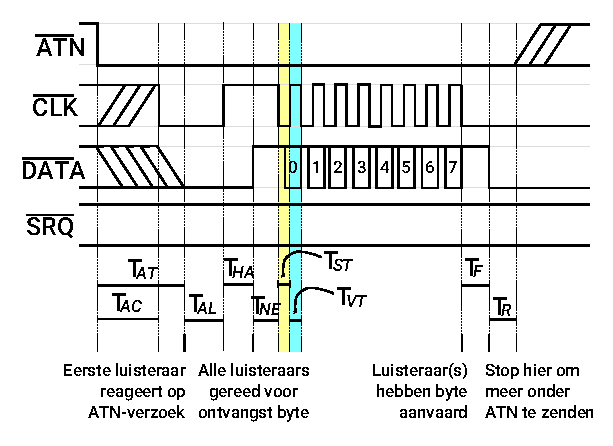
\includegraphics{dutch/images/IEC-Timing-Diagrams/IEC-Timing-Diagram-ATN-Send-Byte}
\end{center}

\begin{center}
    \setlength{\def\arraystretch{1.5}\tabcolsep}{6pt}
    \small {
    \begin{longtable}{|L{0.6cm}|c|c|c|c|L{6cm}|}
      \hline
        \multicolumn{2}{|c|}{\textbf{Symbool}} & \textbf{Min} & \textbf{4541} & \textbf{Max} & \textbf{Omschrijving} \\
        \hline
        \endhead
        \multicolumn{2}{|c|}{T\textsubscript{AT}} & --  & 1000 & $\infty$ &        Reactietijd van het apparaat op Attention. {\em Een apparaat moet          binnen deze tijd op het ATN-verzoek reageren. Indien geen enkel          apparaat binnen deze tijd reageert, volgt een DEVICE NOT PRESENT-fout.          Apparaten dienen derhalve de typische waarde van 1000          microseconden aan te houden.} \\
        \hline
        \multicolumn{2}{|c|}{T\textsubscript{AC}} & --  & 20 & $\infty$? &        Tijd tussen het laag trekken van ATN en het laag trekken van CLK. \\
        \hline
        \multicolumn{2}{|c|}{T\textsubscript{AL}} & --  & 1000 & $\infty$? &        Tijd tussen de reactie van het eerste apparaat op ATN en het loslaten van CLK        door de controller naar 5V. \\
        \hline
        \multicolumn{2}{|c|}{T\textsubscript{HA}} & -- & 64 ms & $\infty$ & Luisteraar-wachttijd. {\em Het protocol staat een luisteraar toe om gedurende een          willekeurige periode of helemaal niet te wachten. De 4541 staat dit niet toe          bij ATN-verzoeken.} \\
        \hline
        \multicolumn{2}{|c|}{T\textsubscript{NE}} & --  & 40 & 200 &        Niet-EOI-tijdskanaalreactie op ``Gereed voor gegevens''. {\em Indien          dit interval te lang is, wordt de byte als een EOI-byte          geïnterpreteerd en zullen de apparaten een EOI-reactie vereisen (zie T\textsubscript{EI}).} \\
        \hline
        \multicolumn{2}{|c|}{T\textsubscript{ST}} & 20*  & 35 & $\infty$ &        Bitinsteltijd. {\em Wordt aangeduid als T\textsubscript{S} in          de C64 Programmer's Reference Guide.}\\
        \hline
        \multicolumn{2}{|c|}{T\textsubscript{VT}} & 20*  & 35 & $\infty$ &        Bitgeldigheid vasthoudtijd. {\em Wordt aangeduid als          T\textsubscript{V} in de C64 Programmer's Reference Guide.} \\
        \hline
        \multicolumn{2}{|c|}{T\textsubscript{F}} & --  & 1000 & 1000 &        Frame-handshake (bevestiging) time-out. \\
        \hline
        \multicolumn{2}{|c|}{T\textsubscript{R}} & 20  & 200 & $\infty$ &        Tijd tussen het ontvangen van de framebevestiging en        het loslaten van de ATN-lijn naar 5V. \\
        \hline
        \multicolumn{6}{l}{\em Alle tijdseenheden zijn uitgedrukt in microseconden, tenzij          anders aangegeven.} \\        \multicolumn{6}{Y{10cm}}{*{}          De Commodore{\texttrademark} 64 Programmer's Reference          Guide stelt dat T\textsubscript{S} en          T\textsubscript{V} elk een minimumduur van 20 microseconden dienen te hebben.          Onze onderzoeken wijzen uit dat bij communicatie met een          1541 veilige waarden voor          T\textsubscript{ST} en T\textsubscript{VT} dichter bij 70          microseconden liggen.
        }
          \\

    \end{longtable}
    }
\end{center}

\subsection{JiffyDOS{\texttrademark}-protocolaanvraag}

Indien ondersteuning voor de JiffyDOS{\texttrademark}-protocoluitbreiding is ingeschakeld, vraagt de 4541 deze slechts aan tijdens de verzending van TALK- en LISTEN-commando's. Dat wil zeggen: wanneer een byte onder Attention wordt gestuurd die valt in het bereik \$20 -- \$5F.

De SRQ-lijn is niet actief in deze transactie.

Samengevat:

\begin{enumerate}
  \item De byte wordt normaal verzonden, tot het    T\textsubscript{ST}-interval vlak voor het laatste bit (bit 7) van de    byte.  \item In plaats van T\textsubscript{ST} af te wachten, moet de controller    een veel langere periode afwachten, doorgaans 300    microseconden, zodat de luisteraar herkent dat hem    gevraagd wordt of hij het JiffyDOS{\texttrademark}    protocol ondersteunt. De controller laat ook de DATA-lijn naar 5V los.  \item Indien de luisteraar het JiffyDOS{\texttrademark} protocol    ondersteunt, trekt hij DATA naar 0V wanneer hij opmerkt dat de CLK-lijn    gedurende de langere periode laag is gehouden.  \item Nadat de luisteraar DATA lang genoeg op 0V heeft gehouden    om er zeker van te zijn dat de controller dit heeft kunnen    opmerken,    laat hij de DATA-lijn los naar 5V. Het apparaat zal nu het    JiffyDOS{\texttrademark} gebruiken voor de gevraagde TALK- of LISTEN-sessie.  \item De controller noteert of de DATA-lijn naar 0V is getrokken, en    registreert in dat geval dat de luisteraar het    JiffyDOS{\texttrademark}-protocol heeft geselecteerd en dit protocol zal gebruiken voor    de gevraagde TALK- of LISTEN-sessie.  \item De controller stuurt nu het laatste bit van de byte.  \item De controller zorgt ervoor dat de bitwaarde van het databit zichtbaar is op    DATA voordat hij CLK activeert, doorgaans 1 -- 4 microseconden.  \item De controller laat de CLK-lijn los naar 5V om aan de    luisteraar aan te geven dat het laatste databit gereed is.  \item De rest van de byte wordt normaal overgedragen.
\end{enumerate}

\begin{center}
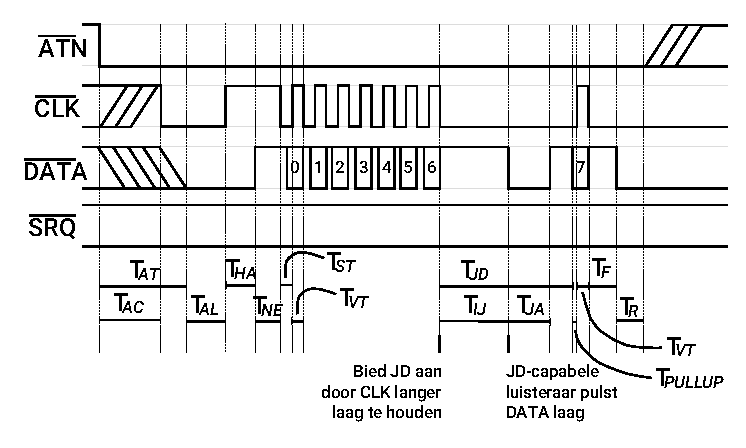
\includegraphics{dutch/images/IEC-Timing-Diagrams/IEC-Timing-Diagram-ATN-JD-Solicit}
\end{center}

\begin{center}
    \setlength{\def\arraystretch{1.5}\tabcolsep}{6pt}
    \small {
    \begin{longtable}{|L{0.6cm}|c|c|c|c|L{6cm}|}
      \hline
        \multicolumn{2}{|c|}{\textbf{Symbool}} & \textbf{Min} & \textbf{4541} & \textbf{Max} & \textbf{Omschrijving} \\
        \hline
        \endhead
        \multicolumn{2}{|c|}{T\textsubscript{JD}} & 320  & 320 & $\infty$ &  Tijd dat CLK op 0V wordt gehouden tussen de twee laatste bits van de byte om het nevenkanaal te markeren; via het nevenkanaal geeft de controller aan dat hij de JiffyDOS{\texttrademark}-protocoluitbeiding wenst te gebruiken.
        \\
        \hline
        \multicolumn{2}{|c|}{T\textsubscript{IJ}} & 100  & -- & 295 &        Tijd voordat de luisteraar de selectie van de JiffyDOS{\texttrademark}-protocoluitbreiding aanvaardt en de bevestiging ervan begint.
        \\
        \hline
        \multicolumn{2}{|c|}{T\textsubscript{IJ}} & 4/100*  & -- & 200 &     Tijd dat de luisteraar de DATA-lijn laag houdt om de selectie van de JiffyDOS{\texttrademark}-protocoluitbreiding te bevestigen.
        \\
        \hline
          \\
\multicolumn{6}{l}{\em Alle tijdseenheden zijn uitgedrukt in microseconden, tenzij anders aangegeven.} \\        \multicolumn{6}{Y{10cm}}{*{}          De 4541 kan pulsbreedtes van slechts 4          microseconden detecteren. Software-implemen\-ta\-ties van het          protocol vereisen echter een grotere waarde. JiffyDOS\texttrademark          gebruikt 100 microseconden.
        }


    \end{longtable}
    }
\end{center}

 \subsection{Verzenden van controller naar apparaat onder JiffyDOS{\texttrademark}}

In tegenstelling tot het standaard seriële protocol maakt het JiffyDOS{\texttrademark}-protocol gebruik van verschillende protocollen voor verzenden en ontvangen. Dit is noodzakelijk bij software-implemen\-ta\-ties om de maximale snelheid te bereiken, omdat de seriële apparaatlijnen op verschillende registerbits zijn gemapt, en een onderdeel van de kracht van het JiffyDOS{\texttrademark}-protocol bestaat uit de slimme manipulatie van de ontvangen bits om het complete byte in de minst mogelijke tijd te reconstrueren, en eveneens bij het verzenden.

Het resultaat is opmerkelijk: JiffyDOS{\texttrademark} kan een byte verzenden in ongeveer dezelfde tijd die het originele protocol nodig heeft om één bit te verzenden!

Let op dat het JiffyDOS{\texttrademark}-protocol databits met de tegenovergestelde polariteit verzendt vergeleken met het standaard protocol: een 1-bit wordt aangegeven met 0V, terwijl een 0-bit wordt aangegeven met 5V.

De SRQ-lijn is niet actief bij deze transactie.

Samengevat:

\begin{enumerate}
 \item Afhankelijk van de toestand van de controller op het moment dat deze met verzenden begint, houdt hij mogelijk de CLK-lijn op 0V. Zo ja, dan laat hij deze onmiddellijk los.\item Vervolgens geeft het apparaat na een willekeurige tijd aan dat het gereed is om een byte van de controller te ontvangen, door de DATA-lijn naar 5V los te laten.\item De timing voor het resterende deel van de byteoverdracht is nu cruciaal, omdat het apparaat direct na het loslaten van DATA de CLK- en DATA-signalen gaat uitlezen om de byte over te dragen.\item De controller wacht enkele microseconden  (T\textsubscript{J6}).\item De controller zet CLK op 0V als databit 4 gelijk is aan 1, en laat deze anders naar 5V los.  De controller zet DATA op 0V als databit 5 gelijk is aan 1, en laat deze anders naar 5V los.\item De controller wacht enkele microseconden  (T\textsubscript{J7}).\item De controller zet CLK op 0V als databit 6 gelijk is aan 1, en laat deze anders naar 5V los.  De controller zet DATA op 0V als databit 7 gelijk is aan 1, en laat deze anders naar 5V los.\item De controller wacht enkele microseconden  (T\textsubscript{J8}).\item De controller zet CLK op 0V als databit 3 gelijk is aan 1, en laat deze anders naar 5V los.  De controller zet DATA op 0V als databit 1 gelijk is aan 1, en laat deze anders naar 5V los.\item De controller wacht enkele microseconden  (T\textsubscript{J9}).\item De controller zet CLK op 0V als databit 2 gelijk is aan 1, en laat deze anders naar 5V los.  De controller zet DATA op 0V als databit 0 gelijk is aan 1, en laat deze anders naar 5V los.\item De controller wacht enkele microseconden  (T\textsubscript{J10}).\item De controller trekt de DATA-lijn naar 0V. Hij laat ook de  CLK-lijn naar 5V los, tenzij hij EOI wil aangeven, in welk  geval hij de CLK-lijn naar 0V trekt.\item De controller wacht enkele microseconden, gedurende welke tijd het  apparaat de EOI-waarde uitleest, en trekt vervolgens DATA naar 0V.  (T\textsubscript{J11}).\item De byteoverdracht is voltooid.
\end{enumerate}

Let er bij het verzenden van de eerste byte onder het JiffyDOS{\texttrademark}protocol op dat het CLK-signaal op 0V kan staan.  De tijd tussen bytes (T\textsubscript{JBB}) is niet vereist (wordt op nul gezet), omdat de korte ontvanglus op het apparaat eenvoudigweg aangeeft wanneer het gereed is om de volgende byte te ontvangen, wat ook bijdraagt aan de hoge snelheid.

Let ook op dat de onderstaande timing gebaseerd is op het moment waarop de signalen ingesteld moeten worden. Bij software-implemen\-ta\-ties moet de latentie van de benodigde processorinstructies in aanmerking worden genomen. Dit vormt geen probleem bij de 4541, omdat deze een latentie van minder dan 50 ns heeft.

\begin{center}
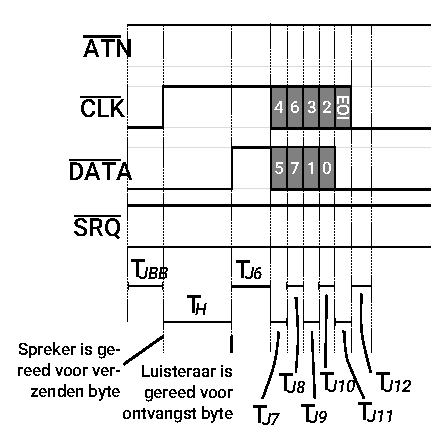
\includegraphics{dutch/images/IEC-Timing-Diagrams/IEC-Timing-Diagram-Send-Byte-JD}
\end{center}

\begin{center}
    \setlength{\def\arraystretch{1.5}\tabcolsep}{6pt}
    \small{
    \begin{longtable}{|L{0.5cm}|c|c|c|c|L{7cm}|}
      \hline
        \multicolumn{2}{|c|}{\textbf{Symbool}} & \textbf{Min} & \textbf{4541} & \textbf{Max} & \textbf{Omschrijving} \\
        \hline
        \endhead
        \multicolumn{2}{|c|}{T\textsubscript{JBB}} & 0  & 0 & $\infty$ &        Tijd tussen bytes.        Er is geen minimale tijd tussen bytes bij het        JiffyDOS{\texttrademark}-protocol,        mits T\textsubscript{J12} voldoende groot is, omdat dat        de latentie van de ontvangroutine effectief verbergt. \\
        \hline
        \multicolumn{2}{|c|}{T\textsubscript{J6}} & 10  & 10 & 10 &        JiffyDOS{\texttrademark} verzenden: insteltijd ontvanger. \\
        \hline
        \multicolumn{2}{|c|}{T\textsubscript{J7}} & 13  & 13 & 13 &        JiffyDOS{\texttrademark} verzenden: vasthoudtijd, eerste di-bit. \\
        \hline
        \multicolumn{2}{|c|}{T\textsubscript{J8}} & 11  & 11 & 11 &        JiffyDOS{\texttrademark} verzenden: vasthoudtijd, tweede di-bit. \\
        \hline
        \multicolumn{2}{|c|}{T\textsubscript{J9}} & 11  & 11 & 11 &        JiffyDOS{\texttrademark} verzenden: vasthoudtijd, derde di-bit. \\
        \hline
        \multicolumn{2}{|c|}{T\textsubscript{J10}} & 12  & 12 & 12 &        JiffyDOS{\texttrademark} verzenden: vasthoudtijd, vierde di-bit. \\
        \hline
        \multicolumn{2}{|c|}{T\textsubscript{J11}} & 15  & 15 & 15 &        JiffyDOS{\texttrademark} verzenden: vasthoudtijd, statusbits. CLK        draagt de EOI-melding, en DATA wordt op 0V gezet om        een succesvolle verzending aan te geven. De ontvanger kan een        framefout aangeven indien DATA 5V wordt waargenomen.  \\
        \hline
        \multicolumn{2}{|c|}{T\textsubscript{J12}} & 18  & 18 & 18 &        JiffyDOS{\texttrademark} hersteltijd na verzending. CLK wordt naar 0V getrokken,        en DATA wordt op 0V gezet om een succesvolle verzending aan te geven.        De ontvanger kan een        framefout aangeven indien DATA 5V wordt waargenomen.  \\
        \hline
        \multicolumn{2}{|c|}{T\textsubscript{JR}} & 15  & 15 & 15 &
        \\
        \hline
        \multicolumn{6}{l}{\em De overige tijden zijn gelijk aan die bij het verzenden van een byte onder Attention.}
          \\
        \multicolumn{6}{l}{\em Alle tijdseenheden zijn uitgedrukt in microseconden, tenzij anders aangegeven.} \\

    \end{longtable}
    }
\end{center}

 \subsection{Ontvangst van randapparaat naar controller onder JiffyDOS{\texttrademark}}

In tegenstelling tot het standaard seriële protocol gebruikt het JiffyDOS{\texttrademark}-protocol verschillende protocollen voor verzenden en ontvangen. Dit is noodzakelijk bij software-implemen\-ta\-ties om de maximale snelheid te bereiken, omdat de seriële randapparatuurbus-lijnen op verschillende registerbits worden gemapt. Een essentieel onderdeel van het JiffyDOS{\texttrademark}-protocol is hoe het op intelligente wijze de ontvangen bits manipuleert om het volledige byte in de kortst mogelijke tijd te reconstrueren, en op vergelijkbare wijze bij verzending.

Het resultaat is opmerkelijk: JiffyDOS{\texttrademark} kan een byte verzenden in ongeveer dezelfde tijd die het originele protocol nodig heeft om één bit te verzenden.

Bij verzending via het JiffyDOS{\texttrademark}-protocol worden de databits geïnverteerd; bij ontvangst van een randapparaat dat het JiffyDOS{\texttrademark}-protocol gebruikt, worden de bits op natuurlijke wijze weergegeven, oftewel met 1 = 5V en 0 = 0V.

De SRQ-lijn is niet actief in deze transactie.

Ter samenvatting:

\begin{enumerate}
\item Het randapparaat kan een willekeurige periode wachten voordat het een byte naar de controller kan verzenden. Wanneer het zover is, laat het de CLK-lijn los naar 5V.\item Wanneer de controller dit opmerkt, laat hij de DATA-lijn los naar 5V en begint het kritieke tijdsgebied van het protocol.\item Het randapparaat wacht kort. Voor apparaten met een software-implemen\-ta\-tie, oftewel alle Commodore{\texttrademark}-stations, is de vertraging een natuurlijk gevolg van de processorinstructie die nodig is om het verzenden van de byte in te luiden; hetzelfde geldt voor de volgende stappen.\item Het randapparaat plaatst het eerste di-bit van gegevens op de CLK- en DATA-lijnen en wacht kort.\item Het randapparaat plaatst het tweede di-bit van gegevens op de CLK- en DATA-lijnen en wacht kort.\item Het randapparaat plaatst het derde di-bit van gegevens op de CLK- en DATA-lijnen en wacht kort.\item Het randapparaat plaatst het vierde di-bit van gegevens op de CLK- en DATA-lijnen en wacht kort.\item Het randapparaat plaatst de statusbits van de byte op de CLK- en DATA-lijnen en wacht kort.\item De controller trekt DATA naar 0V om de ontvangst van de byte te bevestigen en te voorkomen dat het randapparaat nog een byte verzendt voordat hij gereed is.\item Het randapparaat trekt de CLK-lijn naar 0V indien het niet onmiddellijk nog een byte gereed heeft om te verzenden; in het andere geval blijft de lijn op 5V.
\end{enumerate}

De statusbits hebben de volgende betekenis:

\begin{center}
    \setlength{\def\arraystretch{1.5}\tabcolsep}{6pt}
    \begin{longtable}{|c|c|L{7cm}|}
      \hline
        \textbf{CLK} & \textbf{DATA} & \textbf{Betekenis} \\
        \hline
        \endhead
        0V & 0V & Er is een fout opgetreden. \\
        \hline
        0V & 5V & Byte ontvangen met einde-aanduiding (EOI). \\
        \hline
        5V & 0V & Normale byte ontvangen (geen EOI). \\
        \hline
        5V & 5V & Er is een fout opgetreden. \\
        \hline
    \end{longtable}
\end{center}

\begin{center}
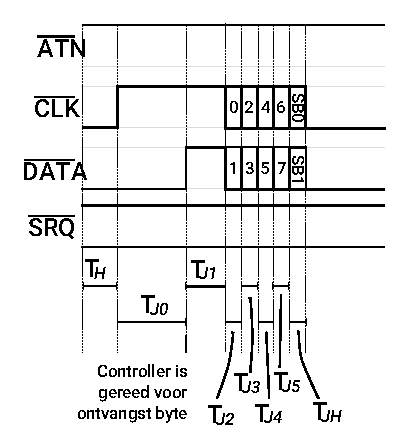
\includegraphics{dutch/images/IEC-Timing-Diagrams/IEC-Timing-Diagram-Receive-Byte-JD}
\end{center}

\begin{center}
    \setlength{\def\arraystretch{1.5}\tabcolsep}{6pt}
    \small{
    \begin{longtable}{|L{0.6cm}|c|c|c|c|L{7cm}|}
      \hline
        \multicolumn{2}{|c|}{\textbf{Symbool}} & \textbf{Min} & \textbf{4541} & \textbf{Max} & \textbf{Omschrijving} \\
        \hline
        \endhead
        \multicolumn{2}{|c|}{T\textsubscript{JH}} & 10  & -- & $\infty$ &        Wachttijd van het randapparaat totdat het gegevens heeft om te verzenden. \\
        \hline
        \multicolumn{2}{|c|}{T\textsubscript{J0}} & 0  & -- & $\infty$ &        Wachttijd van de controller totdat deze gereed is om een byte te ontvangen. \\
        \hline
        \multicolumn{2}{|c|}{T\textsubscript{J1}} & 37  & 37 & $\infty$ &        Deze tijd wordt door soft\-ware-imple\-men\-ta\-ties gebruikt om de byte voor te bereiden voor onmiddellijke verzending. \\
        \hline
        \multicolumn{2}{|c|}{T\textsubscript{J2}} & 14  & 14 & 14 &        Eerste di-bit van gegevens verzenden \\
        \hline
        \multicolumn{2}{|c|}{T\textsubscript{J3}} & 10  & 10 & 10 &        Tweede di-bit van gegevens verzenden \\
        \hline
        \multicolumn{2}{|c|}{T\textsubscript{J4}} & 11  & 11 & 11 &        Derde di-bit van gegevens verzenden \\
        \hline
        \multicolumn{2}{|c|}{T\textsubscript{J5}} & 11  & 11 & 11 &        Vierde di-bit van gegevens verzenden \\
        \hline
        \multicolumn{2}{|c|}{T\textsubscript{JH}} & 13  & 13 & 13 &        Statusbits verzenden \\
        \hline
        \multicolumn{6}{l}{\em De overige tijden zijn gelijk aan die bij het verzenden van een byte onder Attention.}
          \\
        \multicolumn{6}{l}{\em Alle tijdseenheden zijn uitgedrukt in microseconden, tenzij anders aangegeven.} \\

    \end{longtable}
    }
\end{center}



\subsection{Omschakelen van spreker naar luisteraar}

Wanneer de buscontroller een apparaat beveelt om te verzenden, wordt de transactie afgesloten met ATN op 0V. De controller houdt de CLK-lijn op 0V, en het apparaat dat verzond hield de DATA-lijn vast. Deze situatie moet worden omgekeerd: de controller moet de besturing van de bus afstaan en deze overdragen aan het apparaat.

De SRQ-lijn is niet actief bij deze transactie.

Ter samenvatting:

\begin{enumerate}
\item De controller wacht lang genoeg voordat hij de ATN-lijn vrijgeeft, om er zeker van te zijn dat het randapparaat de bevestiging van de byte die onder Attention werd verzonden, heeft afgerond. Dit is de vertraging T\textsubscript{R}.
\item De controller geeft de ATN-lijn vrij naar 5V.
\item De controller wacht enige tijd. Dit is de vertraging T\textsubscript{TK}.
\item De controller geeft de CLK-lijn vrij naar 5V en trekt de DATA-lijn naar 0V. Vanaf dit moment heeft de controller de besturing van de bus afgestaan en wordt hij luisteraar.
\item Na een bepaalde tijdsduur trekt het randapparaat dat op het punt staat te spreken, de CLK-lijn naar 0V en geeft de DATA-lijn vrij, die op 0V blijft staan omdat de controller deze nog steeds naar 0V trekt ter voorbereiding op het ontvangen. Vanaf dit moment is het randapparaat de enige spreker op de bus. De vertraging voordat de CLK-lijn door het randapparaat naar 0V wordt getrokken, is de time-out T\textsubscript{DC}.
\item Het randapparaat wacht enige tijd voordat het met spreken mag beginnen. Dit is de vertraging T\textsubscript{DA}.
\end{enumerate}

Na voltooiing van dit proces zijn de rollen van controller en randapparaat omgekeerd, waarbij het randapparaat nu de rol van spreker (``\textbf{talk}er'') heeft en de controller (en mogelijk andere apparaten op de bus) die van luisteraar (``\textbf{listen}er'').

\begin{center}
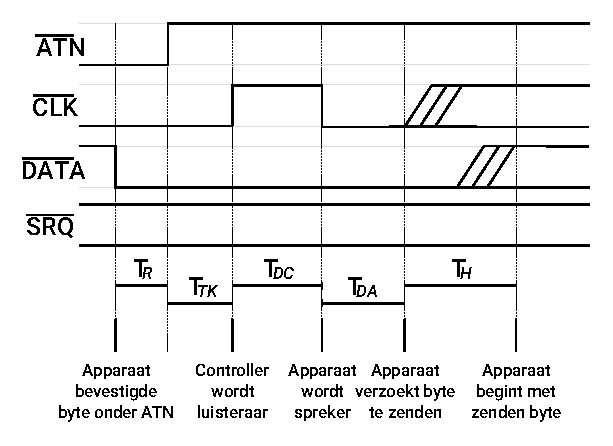
\includegraphics{dutch/images/IEC-Timing-Diagrams/IEC-Timing-Diagram-TurnAround}
\end{center}

\begin{center}
    \setlength{\def\arraystretch{1.5}\tabcolsep}{6pt}
    \small{
    \begin{longtable}{|L{0.6cm}|c|c|c|c|L{6cm}|}
      \hline
        \multicolumn{2}{|c|}{\textbf{Symbool}} & \textbf{Min} & \textbf{4541} & \textbf{Max} & \textbf{Omschrijving} \\
        \hline
        \endhead
        \multicolumn{2}{|c|}{T\textsubscript{DA}} & 4/80* & -- & $\infty$ &        Duur van de bevestiging dat apparaat nu spreker is. De controller houdt CLK.
        \\
        \hline
        \multicolumn{2}{|c|}{T\textsubscript{DC}} & 0 & 64 ms & $\infty$ &        Duur van de zendbevestiging, d.w.z. de tijd die een randapparaat heeft        voordat het spreker wordt. {\em Kan onmiddellijk beginnen zodra CLK op 5V        wordt waargenomen.}\\
        \hline
        \multicolumn{2}{|c|}{T\textsubscript{H}} & -- & N/A & $\infty$ & Luisteraar-wachttijd. {\em De luisteraar kan de ontvangstbevestiging willekeurig lang uitstellen of ook helemaal niet.} \\
        \hline
        \multicolumn{2}{|c|}{T\textsubscript{R}} & 0/20\^{} & 200 & -- & Tijd van        frame tot vrijgave van ATN. \\
        \hline
        \multicolumn{2}{|c|}{T\textsubscript{TK}} & 20 & 40 & 100 & Vrijgave van de        zendvoorwaarde. \\
        \hline
        \multicolumn{6}{l}{\em Alle tijdseenheden zijn uitgedrukt in microseconden, tenzij anders aangegeven.} \\        \multicolumn{6}{Y{10cm}}{* T\textsubscript{DA} wordt geleverd door het randapparaat, niet door de controller. De 4541 is          in staat veel sneller op seriële bus-gebeurtenissen te reageren dan een C64          en heeft derhalve slechts 4 microseconden nodig om te garanderen dat de CLK-lijn          de tijd heeft om naar 5V te stijgen.          Voor controllers met een          softwarematige implementatie van het protocol, zoals de C64,          bedraagt het minimum 80 microseconden.          Randapparaten dienen derhalve steeds          een waarde van ten minste 80 microseconden voor T\textsubscript{DA} te gebruiken.
        } \\
        \multicolumn{6}{Y{10cm}}{\^{} Het          Commodore{\texttrademark} 64 Programmer's Reference Guide          vermeldt          dat T\textsubscript{R} een minimumduur van 20 microseconden heeft.          Wij zien geen aanleiding om te veronderstellen dat          enige implementatie een vertraging vereist          voordat de ATN-lijn kan worden vrijgegeven na het overdragen van          een byte.
        }
          \\
    \end{longtable}
    }
\end{center}

\subsection{Byte verzenden met einde-aanduiding (EOI)}

Na het verzenden van een stroom gegevens wil een apparaat de luisteraar (``\textbf{listen}er'') er vaak van op de hoogte brengen dat het einde van de gegevens is bereikt, bijvoorbeeld zodat deze met de verwerking kan beginnen.  Dit gebeurt door de byte op een bijzondere manier te markeren met het einde-aanduiding (EOI)-attribuut.

Over de betekenis van de afkorting EOI bestaat spraakverwarring. Op de parallele IEE-488 bus heet één van de pinnen in de aansluiting {\em end or identify}. Deze pin heeft inderdaad een dubbele functie: Als ATN niet actief is, dan dient de pin als einde-aanduiding ({\em end}). Is ATN wel actief, dan dient de pin om parallel de status van apparaten op te vragen ({\em identify}). Op de seriële Commodore-bus is de {\em identify}-functie niet aanwezig en is EOI te allen tijde een einde-aanduiding. Wellicht hierom wordt EOI, zelfs in officiële Commodore-documenten, vaak beschreven als {\em end of indicator}.
De meest triviale manier om dit te lezen, "einde van (een) aanduiding", is logisch onzinnig. De juiste manier om dit te lezen is "eind van"-aanduiding, de aanduiding van het eind van gegevensoverdracht. Dit is weer een mooi voorbeeld waarin begrippen in de Engelse taal voor meerdere uitleg vatbaar zijn. We zullen deze spraakverwarring niet meenemen naar het Nederlands en in de handleiding stelselmatig "einde-aanduiding (EOI)" gebruiken.

De einde-aanduiding wordt gerealiseerd met behulp van een timing-nevenkanaal, zodat er geen afzonderlijke ader in de kabel voor nodig is. Wanneer de spreker de CLK-lijn naar 5V heeft gebracht om aan te geven dat hij een byte wil verzenden, en de luisteraar de DATA-lijn naar 5V heeft gebracht om zijn bereidheid om te ontvangen aan te geven, kan de spreker ten minste 200 microseconden wachten om de luisteraar aan te geven dat de byte met EOI-status moet worden ontvangen.  De luisteraar bevestigt dit aan de spreker door de DATA-lijn enige tijd naar 0V te trekken, waarna de verzending vrijwel identiek aan een normale transactie verloopt.

De SRQ-lijn is niet actief bij deze transactie.

Ter samenvatting:

\begin{enumerate}
\item De spreker geeft de CLK-lijn vrij naar 5V om aan te geven dat hij een byte wil verzenden.
\item Na een willekeurige tijdsduur geeft de luisteraar de DATA-lijn vrij naar 5V om zijn bereidheid om een byte te ontvangen aan te geven.
\item Normaal zou de spreker op dit punt na een korte tijd beginnen met het verzenden van de bits.  Om EOI aan te geven, wacht hij evenwel stilzwijgend totdat de luisteraar doorheeft dat deze byte afwijkend is, hetgeen ertoe leidt dat de luisteraar de DATA-lijn terug naar 0V trekt.
\item De luisteraar houdt de DATA-lijn lang genoeg op 0V om er zeker van te zijn dat de spreker dit heeft opgemerkt, en geeft deze vervolgens weer vrij.
\item Zodra de spreker heeft waargenomen dat de luisteraar de DATA-lijn naar 0V heeft getrokken en weer heeft vrijgegeven, begint hij de byte na een korte vertraging normaal te verzenden.
\item Indien de spreker te lang wacht, neemt de luisteraar aan dat de spreker EOI wilde aangeven zonder daadwerkelijk een byte te verzenden.  \item De verzending van de byte wordt op dezelfde manier afgerond als bij een niet-EOI-byte.
\end{enumerate}


\begin{center}
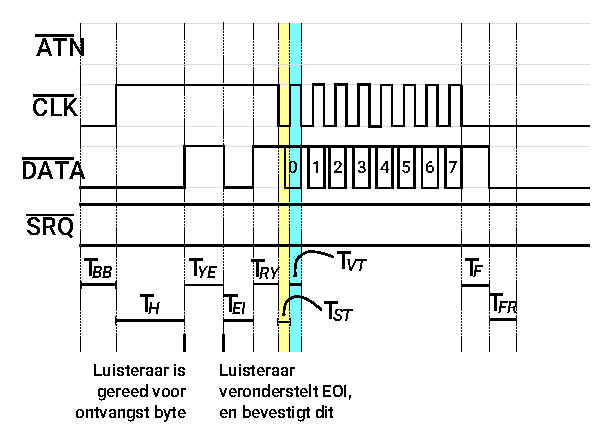
\includegraphics{dutch/images/IEC-Timing-Diagrams/IEC-Timing-Diagram-Send-Byte-EOI}
\end{center}

\begin{center}
    \setlength{\def\arraystretch{1.5}\tabcolsep}{6pt}
    \small{
    \begin{longtable}{|L{0.6cm}|c|c|c|c|L{6cm}|}
      \hline
        \multicolumn{2}{|c|}{\textbf{Symbool}} & \textbf{Min} & \textbf{4541} & \textbf{Max} & \textbf{Omschrijving} \\
        \hline
        \endhead
        \multicolumn{2}{|c|}{T\textsubscript{BB}} & 100 & 100 & $\infty$ &        Tijd tussen bytes. Sprekers moeten lang genoeg wachten om de luisteraar de tijd te geven het einde van de verzending van        de vorige byte te registreren, voordat de volgende byte kan worden verzonden. \\
        \hline
        \multicolumn{2}{|c|}{T\textsubscript{H}} & -- & N/A & $\infty$ & Luisteraar-wachttijd. {\em De luisteraar kan de ontvangstbevestiging willekeurig lang uitstellen of ook helemaal niet.} \\
        \hline
         \multicolumn{2}{|c|}{T\textsubscript{YE}} & 200 & 250 & $\infty$ &        EOI-indicatievertraging. De zender moet ten minste 200        microseconden wachten zodat de ontvanger kan herkennen dat een byte        met EOI wordt verzonden. Indien de vertraging korter is,        herkent de ontvanger de EOI niet. \\
        \hline
         \multicolumn{2}{|c|}{T\textsubscript{EI}} & 60 & 80 & $\infty$ &        EOI-bevestiging vasthoudtijd. De ontvanger moet de DATA-lijn ten minste 60 microseconden weer op 0V trekken, zodat de        zender deze EOI-bevestigingspuls kan detecteren. \\
        \hline
         \multicolumn{2}{|c|}{T\textsubscript{RY}} & 60 & 80 & 100 &        De spreker dient binnen een strak tijdvenster te reageren. Indien hij te vroeg is, is het mogelijk dat de luisteraar zich na bevestiging van de EOI, nog niet heeft voorbereid op ontvangst en kan de synchronisatie verloren gaan. Indien hij te laat is, dan kan de luisteraar concluderen dat de spreker gestopt is met spreken. \\
        \hline
         \multicolumn{2}{|c|}{T\textsubscript{ST}} & 20*  & 35 & $\infty$ &        Databit-insteltijd. {\em In de C64 Programmer's Reference Guide          aangeduid als T\textsubscript{S}.}\\
        \hline
         \multicolumn{2}{|c|}{T\textsubscript{VT}} & 20*  & 35 & $\infty$ &        Databit-geldigheidsvasthoudtijd. {\em In de C64 Programmer's          Reference Guide aangeduid als          T\textsubscript{V}.} \\
        \hline
         \multicolumn{2}{|c|}{T\textsubscript{F}} & --  & 1000 & 1000 &        Frame-handshake (bevestiging) time-out. \\
        \hline
         \multicolumn{2}{|c|}{T\textsubscript{FR}} & 0/60\^ & 0 & $\infty$ &        EOI-frame-bevestiging. De luisteraar trekt DATA na een        korte periode naar 0V om de met EOI verzonden byte te bevestigen. \\
        \hline
         \multicolumn{6}{l}{\em Alle tijdseenheden zijn uitgedrukt in microseconden, tenzij anders aangegeven.} \\        \multicolumn{6}{Y{10cm}}{* T\textsubscript{ST} wordt          geleverd door het randapparaat, niet door de controller. De 4541 is          in staat veel sneller te reageren op seriële bus-gebeurtenissen dan een C64,          en heeft derhalve slechts 4 microseconden nodig om er zeker van te zijn dat          de CLK-lijn de tijd heeft gehad naar 5V te stijgen.          Voor controllers die een softwarematige implementatie          van het protocol gebruiken, zoals de C64,          bedraagt het minimum 80 microseconden.          Randapparaten dienen derhalve altijd een          waarde van ten minste 80 microseconden voor T\textsubscript{DA}          te gebruiken.
        } \\
         \multicolumn{6}{Y{10cm}}{\^{} De          Commodore{\texttrademark} 64 Programmer's Reference Guide          vermeldt          T\textsubscript{FR} met een minimumduur van 60 microseconden.          Wij zien geen enkel bewijs          dat er een vertraging nodig zou zijn          voordat de DATA-lijn door de luisteraar laag kan worden getrokken          om ontvangst van een byte te bevestigen.
        }
          \\
    \end{longtable}
    }
\end{center}

 \subsection{Byte ontvangen}

 Het ontvangen van bytes op de IEC-bus verloopt identiek aan het verzenden.        Het belangrijkste verschil is dat de 4541 veel ruimere        marginale waarden voor tijdsparameters toelaat dan softwarematige implementaties van het bus-protocol. De 4541 heeft niet meer dan 4 microseconden nodig voor een        willekeurige bus-toestand; dit is de tijd die de pull-up-weerstanden        op de bus nodig hebben om de lijnen te laten terugkeren naar 5V.        Intern is de 4541 in staat bit-tijden korter dan 1 microseconde te detecteren.

 \section{Optionele geïntegreerde datalogger}

 De 4541 is verkrijgbaar in een variant die een ingebouwde seriële        randapparatuurbus-datalogger bevat. Deze is ontworpen om het oplossen van        protocolfouten op deze bus te vergemakkelijken. Het vastleggen van gegevens begint zodra        opdracht \$D0 aan de 4541 wordt gegeven, en        duurt ongeveer 4 milliseconden.

\begin{itemize}
   \item {\bf DATALOG0} Het lage byte van de optionele geïntegreerde seriële    randapparatuurbus-datalogger. Het schrijven van \$00 naar dit register    reset het leespunt van de datalogger naar het begin van de    opname. Het schrijven van \$01 naar dit register    verplaatst het leespunt van de datalogger met één tijdstap.    De tijdstappen bedragen ongeveer 1 microseconde, met extra        tijdstappen wanneer een van de signalen op de seriële        perifere bus van toestand verandert.    \item {\bf DATALOG1} Het hoge byte van de optionele geïntegreerde seriële      randapparatuurbus-datalogger. Verschillende velden kunnen op dit      adres worden gelezen door de volgende waarden naar het DATALOG0-register te schrijven:
      \begin{itemize}
         \item \$02 - Lees lage byte van het statemachine-toestandsnummer van de IEC-controller.        \item \$03 - Lees hoge byte van het statemachine-toestandsnummer van de IEC-controller.        \item \$04 - Lees lage byte van het aantal cycli dat de vorige bustoestand        is vastgehouden.        \item \$05 - Lees hoge byte van het aantal cycli dat de vorige bustoestand        is vastgehouden.
        \end{itemize}
\end{itemize}

 Elke tijdstap legt 16 bits informatie vast over de seriële        perifere bus:
\begin{itemize}
 \item {\bf DATALOG0 Bit 0} DATA-lijn invoerwaarde\item {\bf DATALOG0 Bit 1} CLK-lijn invoerwaarde\item {\bf DATALOG0 Bit 2} SRQ-lijn invoerwaarde\item {\bf DATALOG0 Bit 3} DATA-lijn uitvoertoestand\item {\bf DATALOG0 Bit 4} CLK-lijn uitvoertoestand\item {\bf DATALOG0 Bit 5} SRQ-lijn uitvoertoestand\item {\bf DATALOG0 Bit 6} ATN-lijn uitvoertoestand\item {\bf DATALOG0 Bit 7} RESET-lijn uitvoertoestand\item {\bf DATALOG1} Toegang tot de aanvullende datalogger-velden.
\end{itemize}

 De invoerwaarden zijn de spanningen die de 4541 op de        betreffende pinnen uitleest. Los daarvan legt de datalogger vast of de 4541        een van die lijnen laag trekt. Dit maakt het mogelijk te bepalen of        een aangesloten randapparaat of de 4541 een bepaald signaal laag        trekt. Dit biedt veel meer informatie dan het simpelweg signalen        op de seriële randapparatuurbus meten, waarbij niet eenvoudig is vast te stellen wie        een bepaalde lijn laag trekt.

 De volgende waarheidstabel legt uit hoe deze signalen moeten worden geïnterpreteerd:

\begin{center}
    \setlength{\def\arraystretch{1.5}\tabcolsep}{6pt}
    \small{
    \begin{longtable}{|c|c|L{8cm}|}
        \hline
         \textbf{Invoerwaarde} & \textbf{Uitvoerwaarde} &        \textbf{Betekenis}  \\
        \hline
        \endhead
         1 & 1 & Het signaal zweeft op 5V. Geen enkel apparaat trekt het laag. \\
        \hline
         0 & 1 & Het signaal staat op 0V. De 4541 trekt het niet laag, ofwel een aangesloten randapparaat, ofwel de CIA trekt het laag. \\
        \hline
         0 & 0 & Het signaal staat op 0V. De 4541 trekt het laag. Andere apparaten kunnen het ook laag trekken, maar tussen deze twee situaties kan niet worden onderscheiden. \\
        \hline
         1 & 0 & Het signaal zweeft op 5V, maar de 4541 trekt het naar 0V. Uw computer is waarschijnlijk defect, of iemand heeft 5V op het signaal aangesloten zonder stroombeperkende        weerstand ertussen; in dat geval is uw computer op het punt defect te raken. \\
        \hline
    \end{longtable}
    }
\end{center}

\subsection{Gegevens uit de datalogger halen}

Met het volgende programma wordt de inhoud van de datalogger opgehaald en als PETSCII-golfvorm weergegeven, zoals de hier getoonde:

\begin{center}
  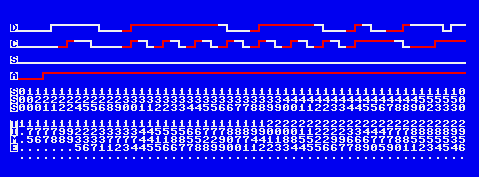
\includegraphics[width=0.7\linewidth]{images/IEC-Timing-Diagrams/iec-waveform-cropped}
\end{center}


% Program is too long to fit on a single page
\input{examples/iec-data-logger}
\input{examples/iec-data-logger-2}

  \input{dutch/appendix-sound-registers}
  \chapter{Registers van de real-time klok (RTC)}

\section{Algemene RTC-registers (alle revisies)}
\setlength{\tabcolsep}{0pt}
\begin{longtable}{|C{16.5mm}|C{12.5mm}|C{12.5mm}|C{12.5mm}|C{12.5mm}|C{12.5mm}|C{12.5mm}|C{12.5mm}|C{12.5mm}|}
\hline
{\bf{HEX}} & {\bf{DB7}} & {\bf{DB6}} & {\bf{DB5}} & {\bf{DB4}} & {\bf{DB3}} & {\bf{DB2}} & {\bf{DB1}} & {\bf{DB0}} \\
\hline
\endfirsthead
\multicolumn{3}{l@{}}{\ldots vervolgd}\\
\hline
{\bf{HEX}} & {\bf{DB7}} & {\bf{DB6}} & {\bf{DB5}} & {\bf{DB4}} & {\bf{DB3}} & {\bf{DB2}} & {\bf{DB1}} & {\bf{DB0}} \\
\endhead
\multicolumn{3}{l@{}}{vervolgd \ldots}\\
\endfoot
\hline
\endlastfoot
\footnotesize  FFD7110\index{Registers!\$FFD7110} & \multicolumn{8}{c|}{\footnotesize RTCSEC\index{Registers!RTCSEC}}\\
\hline
\footnotesize  FFD7111\index{Registers!\$FFD7111} & \multicolumn{8}{c|}{\footnotesize RTCMIN\index{Registers!RTCMIN}}\\
\hline
\footnotesize  FFD7112\index{Registers!\$FFD7112} & \footnotesize Ongebruikt & \multicolumn{7}{c|}{\footnotesize RTC\-HOUR\index{Registers!RTCHOUR}}\\
\hline
\footnotesize  FFD7113\index{Registers!\$FFD7113} & \multicolumn{8}{c|}{\footnotesize RTCDAY\index{Registers!RTCDAY}}\\
\hline
\footnotesize  FFD7114\index{Registers!\$FFD7114} & \multicolumn{8}{c|}{\footnotesize RTCMONTH\index{Registers!RTCMONTH}}\\
\hline
\footnotesize  FFD7115\index{Registers!\$FFD7115} & \multicolumn{8}{c|}{\footnotesize RTCYEAR\index{Registers!RTCYEAR}}\\
\hline
\footnotesize  FFD7116\index{Registers!\$FFD7116} & \multicolumn{8}{c|}{\footnotesize RTCDOW\index{Registers!RTCDOW}}\\
\hline
\footnotesize  FFD7140 -- FFD717F\index{Registers!\$FFD7140 -- \$FFD717F} & \multicolumn{8}{c|}{\footnotesize NVRAM\index{Registers!NVRAM}}\\
\hline
\end{longtable}
\begin{itemize}
\item{\bf{NVRAM}\index{Registers!NVRAM}} 64 byte niet-vluchtig RAM; kan worden gebruikt om de machineconfiguratie op te slaan
\item{\bf{RTCDAY}\index{Registers!RTCDAY}} Waarde die de dag van de maand aangeeft in de realtimeklok (binair gecodeerd decimaal)
\item{\bf{RTCDOW}\index{Registers!RTCDOW}} Waarde die de dag van de week aangeeft in de realtimeklok (0-6; binair gecodeerd decimaal)
\item{\bf{RTCHOUR}\index{Registers!RTCHOUR}} Waarde die het uur aangeeft in de realtimeklok (binair gecodeerd decimaal)
\item{\bf{RTCHOUR24EN}\index{Registers!RTCHOUR24EN}} Schakelt de 24-uursmodus van de realtimeklok in
\item{\bf{RTCHOURPM}\index{Registers!RTCHOURPM}} PM-indicator van de realtimeklok (alleen in de 12-uursmodus)
\item{\bf{RTCMIN}\index{Registers!RTCMIN}} Waarde die de minuten aangeeft in de realtimeklok (binair gecodeerd decimaal)
\item{\bf{RTCMONTH}\index{Registers!RTCMONTH}} Waarde die de maand aangeeft in de realtimeklok (binair gecodeerd decimaal)
\item{\bf{RTCSEC}\index{Registers!RTCSEC}} Waarde die de seconden aangeeft in de realtimeklok (binair gecodeerd decimaal)
\item{\bf{RTCYEAR}\index{Registers!RTCYEAR}} Waarde die het jaar aangeeft in de realtimeklok (binair gecodeerd decimaal)
\item{\bf{Ongebruikt}\index{Registers!Ongebruikt}} Ongebruikt; altijd 1
\end{itemize}


\section{Uitgebreide RTC-registers (moederbord R4 en nieuwer)}Deze moederborden bevatten de RV-3032-C7, welke enkele extra registers biedt. Lees de documentatie voor deze RTC-chip zorgvuldig door voordat u deze registers wijzigt!

\setlength{\tabcolsep}{0pt}
\begin{longtable}{|C{16.5mm}|C{12.5mm}|C{12.5mm}|C{12.5mm}|C{12.5mm}|C{12.5mm}|C{12.5mm}|C{12.5mm}|C{12.5mm}|}
\hline
{\bf{HEX}} & {\bf{DB7}} & {\bf{DB6}} & {\bf{DB5}} & {\bf{DB4}} & {\bf{DB3}} & {\bf{DB2}} & {\bf{DB1}} & {\bf{DB0}} \\
\hline
\endfirsthead
\multicolumn{3}{l@{}}{\ldots vervolgd}\\
\hline
{\bf{HEX}} & {\bf{DB7}} & {\bf{DB6}} & {\bf{DB5}} & {\bf{DB4}} & {\bf{DB3}} & {\bf{DB2}} & {\bf{DB1}} & {\bf{DB0}} \\
\endhead
\multicolumn{3}{l@{}}{vervolgd \ldots}\\
\endfoot
\hline
\endlastfoot
\footnotesize  FFD7116\index{Registers!\$FFD7116} & \multicolumn{8}{c|}{\footnotesize RTCDOW\index{Registers!RTCDOW}}\\
\hline
\footnotesize  FFD7117\index{Registers!\$FFD7117} & \multicolumn{8}{c|}{\footnotesize 100THSEC\index{Registers!100THSEC}}\\
\hline
\footnotesize  FFD7118\index{Registers!\$FFD7118} & \footnotesize AE\_M & \multicolumn{7}{c|}{\footnotesize ALMINUTES\index{Registers!ALMINUTES}}\\
\hline
\footnotesize  FFD7119\index{Registers!\$FFD7119} & \footnotesize AE\_H & \footnotesize -- & \multicolumn{6}{c|}{\footnotesize ALHOURS\index{Registers!ALHOURS}}\\
\hline
\footnotesize  FFD711A\index{Registers!\$FFD711A} & \footnotesize AE\_D & \footnotesize -- & \multicolumn{6}{c|}{\footnotesize ALDAY\index{Registers!ALDAY}}\\
\hline
\footnotesize  FFD711B\index{Registers!\$FFD711B} & \multicolumn{8}{c|}{\footnotesize PCTCR0\index{Registers!PCTCR0}}\\
\hline
\footnotesize  FFD711C\index{Registers!\$FFD711C} & \multicolumn{4}{c|}{\footnotesize --}& \multicolumn{4}{c|}{\footnotesize PCTCR1\index{Registers!PCTCR1}}\\
\hline
\footnotesize  FFD711D\index{Registers!\$FFD711D} & \footnotesize THF & \footnotesize TLF & \footnotesize UF & \footnotesize TF & \footnotesize AF & \footnotesize EVF & \footnotesize PORF & \footnotesize VLF \\
\hline
\footnotesize  FFD711E\index{Registers!\$FFD711E} & \multicolumn{4}{c|}{\footnotesize TEMPL\index{Registers!TEMPL}}& \footnotesize EEF & \footnotesize EEbusy & \footnotesize CLKF & \footnotesize BSF \\
\hline
\footnotesize  FFD711F\index{Registers!\$FFD711F} & \multicolumn{8}{c|}{\footnotesize TEMPH\index{Registers!TEMPH}}\\
\hline
\footnotesize  FFD7120\index{Registers!\$FFD7120} & \footnotesize Ongebruikt & \footnotesize Ongebruikt & \footnotesize GP0 & \footnotesize USEL & \footnotesize TE & \footnotesize EERD & \multicolumn{2}{c|}{\footnotesize TD\index{Registers!TD}}\\
\hline
\footnotesize  FFD7121\index{Registers!\$FFD7121} & \footnotesize -- & \footnotesize CLKIE & \footnotesize UIE & \footnotesize TIE & \footnotesize AIE & \footnotesize EIE & \footnotesize GP1 & \footnotesize STOP \\
\hline
\footnotesize  FFD7122\index{Registers!\$FFD7122} & \multicolumn{3}{c|}{\footnotesize Ongebruikt\index{Registers!Ongebruikt}}& \footnotesize BSIE & \footnotesize THE & \footnotesize TLE & \footnotesize THIE & \footnotesize TLIE \\
\hline
\footnotesize  FFD7123\index{Registers!\$FFD7123} & \multicolumn{2}{c|}{\footnotesize Ongebruikt\index{Registers!Ongebruikt}}& \footnotesize EVR & \footnotesize THR & \footnotesize TLR & \footnotesize EVOW & \footnotesize THOW & \footnotesize TLOW \\
\hline
\footnotesize  FFD7124\index{Registers!\$FFD7124} & \footnotesize CLKD & \footnotesize INTDE & \footnotesize CEIE & \footnotesize CAIE & \footnotesize CTIE & \footnotesize CUIE & \footnotesize CTHIE & \footnotesize CTLIE \\
\hline
\footnotesize  FFD7125\index{Registers!\$FFD7125} & \footnotesize CLKDE & \footnotesize EHL & \multicolumn{2}{c|}{\footnotesize ET\index{Registers!ET}}& \multicolumn{3}{c|}{\footnotesize Ongebruikt\index{Registers!Ongebruikt}}& \footnotesize ESYN \\
\hline
\footnotesize  FFD7126\index{Registers!\$FFD7126} & \multicolumn{8}{c|}{\footnotesize TLT\index{Registers!TLT}}\\
\hline
\footnotesize  FFD7127\index{Registers!\$FFD7127} & \multicolumn{8}{c|}{\footnotesize THT\index{Registers!THT}}\\
\hline
\footnotesize  FFD7128\index{Registers!\$FFD7128} & \multicolumn{8}{c|}{\footnotesize TSTLowCount\index{Registers!TSTLowCount}}\\
\hline
\footnotesize  FFD7129\index{Registers!\$FFD7129} & \footnotesize -- & \multicolumn{7}{c|}{\footnotesize TSTLowSec\index{Registers!TSTLowSec}}\\
\hline
\footnotesize  FFD712A\index{Registers!\$FFD712A} & \footnotesize -- & \multicolumn{7}{c|}{\footnotesize TSTLowMin\index{Registers!TSTLowMin}}\\
\hline
\footnotesize  FFD712B\index{Registers!\$FFD712B} & \multicolumn{2}{c|}{\footnotesize --}& \multicolumn{6}{c|}{\footnotesize TSTLowHrs\index{Registers!TSTLowHrs}}\\
\hline
\footnotesize  FFD712C\index{Registers!\$FFD712C} & \multicolumn{2}{c|}{\footnotesize --}& \multicolumn{6}{c|}{\footnotesize TSTLowDat\index{Registers!TSTLowDat}}\\
\hline
\footnotesize  FFD712D\index{Registers!\$FFD712D} & \multicolumn{3}{c|}{\footnotesize --}& \multicolumn{5}{c|}{\footnotesize TSTLowMonth\index{Registers!TSTLowMonth}}\\
\hline
\footnotesize  FFD712E\index{Registers!\$FFD712E} & \multicolumn{8}{c|}{\footnotesize TSTLowYear\index{Registers!TSTLowYear}}\\
\hline
\footnotesize  FFD712F\index{Registers!\$FFD712F} & \multicolumn{8}{c|}{\footnotesize TSTHighCount\index{Registers!TSTHighCount}}\\
\hline
\footnotesize  FFD7130\index{Registers!\$FFD7130} & \footnotesize -- & \multicolumn{7}{c|}{\footnotesize TSTHighSec\index{Registers!TSTHighSec}}\\
\hline
\footnotesize  FFD7131\index{Registers!\$FFD7131} & \footnotesize -- & \multicolumn{7}{c|}{\footnotesize TSTHighMin\index{Registers!TSTHighMin}}\\
\hline
\footnotesize  FFD7132\index{Registers!\$FFD7132} & \multicolumn{2}{c|}{\footnotesize --}& \multicolumn{6}{c|}{\footnotesize TSTHighHrs\index{Registers!TSTHighHrs}}\\
\hline
\footnotesize  FFD7133\index{Registers!\$FFD7133} & \multicolumn{2}{c|}{\footnotesize --}& \multicolumn{6}{c|}{\footnotesize TSTHighDat\index{Registers!TSTHighDat}}\\
\hline
\footnotesize  FFD7134\index{Registers!\$FFD7134} & \multicolumn{3}{c|}{\footnotesize --}& \multicolumn{5}{c|}{\footnotesize TSTHighMonth\index{Registers!TSTHighMonth}}\\
\hline
\footnotesize  FFD7135\index{Registers!\$FFD7135} & \multicolumn{8}{c|}{\footnotesize TSTHighYear\index{Registers!TSTHighYear}}\\
\hline
\footnotesize  FFD7136\index{Registers!\$FFD7136} & \multicolumn{8}{c|}{\footnotesize TSEVICount\index{Registers!TSEVICount}}\\
\hline
\footnotesize  FFD7137\index{Registers!\$FFD7137} & \multicolumn{8}{c|}{\footnotesize TSEVI100th\index{Registers!TSEVI100th}}\\
\hline
\footnotesize  FFD7138\index{Registers!\$FFD7138} & \footnotesize -- & \multicolumn{7}{c|}{\footnotesize TSEVISec\index{Registers!TSEVISec}}\\
\hline
\footnotesize  FFD7139\index{Registers!\$FFD7139} & \footnotesize -- & \multicolumn{7}{c|}{\footnotesize TSEVIMin\index{Registers!TSEVIMin}}\\
\hline
\footnotesize  FFD713A\index{Registers!\$FFD713A} & \multicolumn{2}{c|}{\footnotesize --}& \multicolumn{6}{c|}{\footnotesize TSEVIHrs\index{Registers!TSEVIHrs}}\\
\hline
\footnotesize  FFD713B\index{Registers!\$FFD713B} & \multicolumn{2}{c|}{\footnotesize --}& \multicolumn{6}{c|}{\footnotesize TSEVIDat\index{Registers!TSEVIDat}}\\
\hline
\footnotesize  FFD713C\index{Registers!\$FFD713C} & \multicolumn{3}{c|}{\footnotesize --}& \multicolumn{5}{c|}{\footnotesize TSEVIMonth\index{Registers!TSEVIMonth}}\\
\hline
\footnotesize  FFD713D\index{Registers!\$FFD713D} & \multicolumn{8}{c|}{\footnotesize TSEVIYear\index{Registers!TSEVIYear}}\\
\hline
\end{longtable}
\begin{itemize}
\item{\bf{100THSEC}\index{Registers!100THSEC}} Honderdsten van seconden van de realtimeklok
\item{\bf{AE\_D}\index{Registers!AE\_D}} Inschakelbit van het alarm (samen met AE\_M en AE\_H)
\item{\bf{AE\_H}\index{Registers!AE\_H}} Inschakelbit van het alarm (samen met AE\_M en AE\_D)
\item{\bf{AE\_M}\index{Registers!AE\_M}} Inschakelbit van het minuten-alarm; schakelt het alarm in samen met AE\_H en AE\_D
\item{\bf{AF}\index{Registers!AF}} Statusregister: 1 geeft het optreden van een alarminterrupt aan
\item{\bf{AIE}\index{Registers!AIE}} Inschakelbit van het alarminterrupt
\item{\bf{ALDAY}\index{Registers!ALDAY}} Datumwaarde van het alarm, 01-31 (binair gecodeerd decimaal)
\item{\bf{ALHOURS}\index{Registers!ALHOURS}} Uurwaarde van het alarm, 00-23 (binair gecodeerd decimaal)
\item{\bf{ALMINUTES}\index{Registers!ALMINUTES}} Minutenwaarde van het alarm, 00-59 (binair gecodeerd decimaal)
\item{\bf{BSF}\index{Registers!BSF}} 1 geeft aan dat een omschakeling van de hoofdvoeding naar de back-up heeft plaatsgevonden
\item{\bf{BSIE}\index{Registers!BSIE}} Inschakelbit van het interrupt voor de back-upomschakeling
\item{\bf{CAIE}\index{Registers!CAIE}} Klokuitvoer wanneer de alarm-interrupt is ingeschakeld
\item{\bf{CEIE}\index{Registers!CEIE}} Klokuitvoer wanneer de EVI-interrupt is ingeschakeld
\item{\bf{CLKD}\index{Registers!CLKD}} Inschakelbit voor de uitschakelvertragingswaarde van CLKOUT na I2C STOP
\item{\bf{CLKDE}\index{Registers!CLKDE}} Inschakelbit van de uitschakelvertraging van CLKOUT na I2C-STOP
\item{\bf{CLKF}\index{Registers!CLKF}} 1 geeft het optreden van een interruptgestuurde klokuitvoer op de CLKOUT-pin aan
\item{\bf{CLKIE}\index{Registers!CLKIE}} Inschakelbit van de interruptgestuurde klokuitvoer
\item{\bf{CTHIE}\index{Registers!CTHIE}} Klokuitvoer wanneer de THigh-interrupt is ingeschakeld
\item{\bf{CTIE}\index{Registers!CTIE}} Klokuitvoer wanneer de interrupt van de periodieke afteltimer is ingeschakeld
\item{\bf{CTLIE}\index{Registers!CTLIE}} Klokuitvoer wanneer de TLow-interrupt is ingeschakeld
\item{\bf{CUIE}\index{Registers!CUIE}} Klokuitvoer wanneer de Periodic Time Update-interrupt is ingeschakeld
\item{\bf{EEF}\index{Registers!EEF}} 1 geeft aan dat de EEPROM-schrijftoegang is mislukt
\item{\bf{EERD}\index{Registers!EERD}} Bit voor het uitschakelen van de EEPROM-geheugenverversing
\item{\bf{EEbusy}\index{Registers!EEbusy}} 1 geeft aan dat de EEPROM momenteel bezig is en verdere commando's negeert
\item{\bf{EHL}\index{Registers!EHL}} Selectie van het hoge/lage niveau van de gebeurtenis (stijgende/dalende flank) voor detectie
\item{\bf{EIE}\index{Registers!EIE}} Inschakelbit voor de interrupt van een externe gebeurtenis
\item{\bf{ESYN}\index{Registers!ESYN}} Synchronisatiebit voor een externe gebeurtenis (EVI)
\item{\bf{ET}\index{Registers!ET}} Instelling van de filtertijd voor gebeurtenissen
\item{\bf{EVF}\index{Registers!EVF}} Statusregister: 1 geeft aan dat een externe gebeurtenis is opgetreden
\item{\bf{EVOW}\index{Registers!EVOW}} Overschrijfbit van de EVI-tijdstempel
\item{\bf{EVR}\index{Registers!EVR}} Resetbit van de EVI-tijdstempel
\item{\bf{GP0}\index{Registers!GP0}} Registerbit voor algemeen gebruik
\item{\bf{GP1}\index{Registers!GP1}} Registerbit voor algemeen gebruik
\item{\bf{INTDE}\index{Registers!INTDE}} Inschakelbit voor interruptvertraging na het inschakelen van CLKOUT
\item{\bf{PCTCR0}\index{Registers!PCTCR0}} Besturingsregister van periodieke afteltimer 0 (lage byte)
\item{\bf{PCTCR1}\index{Registers!PCTCR1}} Besturingsregister van periodieke afteltimer 1 (hoge byte)
\item{\bf{PORF}\index{Registers!PORF}} Statusregister: 1 geeft aan dat gegevens ongeldig zijn vanwege een stroomprobleem; registers moeten opnieuw worden geïnitialiseerd
\item{\bf{RTCDOW}\index{Registers!RTCDOW}} Waarde van de dag van de week, 0-6 (binair gecodeerd decimaal)
\item{\bf{STOP}\index{Registers!STOP}} 1 stopt de timer en herstelt de klokvoorscalerfrequenties
\item{\bf{TD}\index{Registers!TD}} Selectie van de timerklokfrequentie
\item{\bf{TE}\index{Registers!TE}} Inschakelbit van de periodieke afteltimer
\item{\bf{TEMPH}\index{Registers!TEMPH}} Geheel deel van de temperatuurwaarde [11.0] in tweecomplementformaat
\item{\bf{TEMPL}\index{Registers!TEMPL}} Fractiedeel van de temperatuurwaarde [11:0] in tweecomplementformaat
\item{\bf{TF}\index{Registers!TF}} Statusregister: 1 geeft het optreden van een interrupt van de periodieke afteltimer aan
\item{\bf{THE}\index{Registers!THE}} Inschakelbit voor hoge temperatuur
\item{\bf{THF}\index{Registers!THF}} Statusregister: 1 geeft aan dat de temperatuur de hoge drempelwaarde THT heeft overschreden
\item{\bf{THIE}\index{Registers!THIE}} Inschakelbit voor de hoge-temperatuurinterrupt
\item{\bf{THOW}\index{Registers!THOW}} Overschrijfbit van de THigh-tijdstempel
\item{\bf{THR}\index{Registers!THR}} Resetbit van de THigh-tijdstempel
\item{\bf{THT}\index{Registers!THT}} Temperatuurdrempelregister: hoge drempelwaarde (THigh)
\item{\bf{TIE}\index{Registers!TIE}} Inschakelbit voor de interrupt van de periodieke afteltimer
\item{\bf{TLE}\index{Registers!TLE}} Inschakelbit voor lage temperatuur
\item{\bf{TLF}\index{Registers!TLF}} Statusregister: 1 geeft aan dat de temperatuur onder de lage drempelwaarde TLT is gezakt
\item{\bf{TLIE}\index{Registers!TLIE}} Inschakelbit voor de lage-temperatuurinterrupt
\item{\bf{TLOW}\index{Registers!TLOW}} Bit voor het overschrijven van TLow in de tijdstempel.
\item{\bf{TLR}\index{Registers!TLR}} Bit voor het resetten van TLow in de tijdstempel.
\item{\bf{TLT}\index{Registers!TLT}} Temperatuurdrempelregister: lage drempelwaarde (TLow)
\item{\bf{TSEVI100th}\index{Registers!TSEVI100th}} Tijdstempelevenementregister: TS EVI honderdsten van seconden
\item{\bf{TSEVICount}\index{Registers!TSEVICount}} Tijdstempelevenementregister: TS EVI-telling
\item{\bf{TSEVIDat}\index{Registers!TSEVIDat}} Tijdstempel-THigh-register: TS TLow-datum
\item{\bf{TSEVIHrs}\index{Registers!TSEVIHrs}} Tijdstempel-THigh-register: TS TLow-uren
\item{\bf{TSEVIMin}\index{Registers!TSEVIMin}} Tijdstempel-THigh-register: TS TLow-minuten
\item{\bf{TSEVIMonth}\index{Registers!TSEVIMonth}} Tijdstempel-THigh-register: TS TLow-maand
\item{\bf{TSEVISec}\index{Registers!TSEVISec}} Tijdstempel-THigh-register: TS TLow-seconden
\item{\bf{TSEVIYear}\index{Registers!TSEVIYear}} Tijdstempel-THigh-register: TS TLow-jaar
\item{\bf{TSTHighCount}\index{Registers!TSTHighCount}} Tijdstempel-THigh-register: TS TLow-telling
\item{\bf{TSTHighDat}\index{Registers!TSTHighDat}} Tijdstempel-THigh-register: TS TLow-datum
\item{\bf{TSTHighHrs}\index{Registers!TSTHighHrs}} Tijdstempel-THigh-register: TS TLow-uren
\item{\bf{TSTHighMin}\index{Registers!TSTHighMin}} Tijdstempel-THigh-register: TS TLow-minuten
\item{\bf{TSTHighMonth}\index{Registers!TSTHighMonth}} Tijdstempel-THigh-register: TS TLow-maand
\item{\bf{TSTHighSec}\index{Registers!TSTHighSec}} Tijdstempel-THigh-register: TS TLow-seconden
\item{\bf{TSTHighYear}\index{Registers!TSTHighYear}} Tijdstempel-THigh-register: TS TLow-jaar
\item{\bf{TSTLowCount}\index{Registers!TSTLowCount}} Tijdstempel-TLow-register: TS TLow-telling
\item{\bf{TSTLowDat}\index{Registers!TSTLowDat}} Tijdstempel-TLow-register: TS TLow-datum
\item{\bf{TSTLowHrs}\index{Registers!TSTLowHrs}} Tijdstempel-TLow-register: TS TLow-uren
\item{\bf{TSTLowMin}\index{Registers!TSTLowMin}} Tijdstempel-TLow-register: TS TLow-minuten
\item{\bf{TSTLowMonth}\index{Registers!TSTLowMonth}} Tijdstempel-TLow-register: TS TLow-maand
\item{\bf{TSTLowSec}\index{Registers!TSTLowSec}} Tijdstempel-TLow-register: TS TLow-seconden
\item{\bf{TSTLowYear}\index{Registers!TSTLowYear}} Tijdstempel-TLow-register: TS TLow-jaar
\item{\bf{UF}\index{Registers!UF}} Statusregister: 1 geeft aan dat er een periodieke timer-update-interruptgebeurtenis heeft plaatsgevonden.
\item{\bf{UIE}\index{Registers!UIE}} Bit voor het inschakelen van de periodieke tijdupdate-interrupt.
\item{\bf{USEL}\index{Registers!USEL}} Bit voor het selecteren van de update-interrupt
\item{\bf{Ongebruikt}\index{Registers!Ongebruikt}} Niet geïmplementeerd. Geeft altijd 0 terug
\item{\bf{VLF}\index{Registers!VLF}} Statusregister: 1 geeft aan dat er ongeldige gegevens zijn door een voedingsprobleem. De registers moeten opnieuw worden geïnitialiseerd.
\end{itemize}


\section{Registers op de Grove-RTC-vervangingsunit}Deze registers zijn beschikbaar indien een Grove-vervangingsunit is geïnstalleerd. Dit onderdeel is alleen nodig indien uw RTC defect is. Dit heeft alleen betrekking op de eerste R3-moederborden die werden verzonden.

\setlength{\tabcolsep}{0pt}
\begin{longtable}{|C{16.5mm}|C{12.5mm}|C{12.5mm}|C{12.5mm}|C{12.5mm}|C{12.5mm}|C{12.5mm}|C{12.5mm}|C{12.5mm}|}
\hline
{\bf{HEX}} & {\bf{DB7}} & {\bf{DB6}} & {\bf{DB5}} & {\bf{DB4}} & {\bf{DB3}} & {\bf{DB2}} & {\bf{DB1}} & {\bf{DB0}} \\
\hline
\endfirsthead
\multicolumn{3}{l@{}}{\ldots vervolgd}\\
\hline
{\bf{HEX}} & {\bf{DB7}} & {\bf{DB6}} & {\bf{DB5}} & {\bf{DB4}} & {\bf{DB3}} & {\bf{DB2}} & {\bf{DB1}} & {\bf{DB0}} \\
\endhead
\multicolumn{3}{l@{}}{vervolgd \ldots}\\
\endfoot
\hline
\endlastfoot
\footnotesize  FFD7400\index{Registers!\$FFD7400} & \multicolumn{8}{c|}{\footnotesize EXTRTC\-SEC\index{Registers!EXTRTCSEC}}\\
\hline
\footnotesize  FFD7401\index{Registers!\$FFD7401} & \multicolumn{8}{c|}{\footnotesize EXTRTC\-MIN\index{Registers!EXTRTCMIN}}\\
\hline
\footnotesize  FFD7402\index{Registers!\$FFD7402} & \footnotesize -- & \footnotesize EXTRTC\-HOUR12EN & \footnotesize EXTRTC\-HOURPM & \multicolumn{5}{c|}{\footnotesize EXTRTC\-HOUR\index{Registers!EXTRTCHOUR}}\\
\hline
\footnotesize  FFD7403\index{Registers!\$FFD7403} & \multicolumn{8}{c|}{\footnotesize EXTRTC\-DOW\index{Registers!EXTRTCDOW}}\\
\hline
\footnotesize  FFD7404\index{Registers!\$FFD7404} & \multicolumn{8}{c|}{\footnotesize EXTRTC\-DAY\index{Registers!EXTRTCDAY}}\\
\hline
\footnotesize  FFD7405\index{Registers!\$FFD7405} & \footnotesize EXTRTC\-CENTURY & \multicolumn{2}{c|}{\footnotesize --}& \multicolumn{5}{c|}{\footnotesize EXTRTC\-MONTH\index{Registers!EXTRTCMONTH}}\\
\hline
\footnotesize  FFD7406\index{Registers!\$FFD7406} & \multicolumn{8}{c|}{\footnotesize EXTRTC\-YEAR\index{Registers!EXTRTCYEAR}}\\
\hline
\footnotesize  FFD7407\index{Registers!\$FFD7407} & \footnotesize EXTRTC\-A1M1 & \multicolumn{7}{c|}{\footnotesize EXTRTC\-A1SEC\index{Registers!EXTRTCA1SEC}}\\
\hline
\footnotesize  FFD7408\index{Registers!\$FFD7408} & \footnotesize EXTRTC\-A1M2 & \multicolumn{7}{c|}{\footnotesize EXTRTC\-A1MIN\index{Registers!EXTRTCA1MIN}}\\
\hline
\footnotesize  FFD7409\index{Registers!\$FFD7409} & \footnotesize EXTRTC\-A1M3 & \footnotesize EXTRTC\-A1HOUR12EN & \footnotesize EXTRTC\-A1HOURPM & \multicolumn{5}{c|}{\footnotesize EXTRTC\-A1HOUR\index{Registers!EXTRTCA1HOUR}}\\
\hline
\footnotesize  FFD740A\index{Registers!\$FFD740A} & \footnotesize EXTRTC\-A1M4 & \footnotesize EXTRTC\-A1DOWSEL & \multicolumn{6}{c|}{\footnotesize EXTRTC\-A1DATE\index{Registers!EXTRTCA1DATE}}\\
\hline
\footnotesize  FFD740B\index{Registers!\$FFD740B} & \footnotesize EXTRTC\-A2M2 & \multicolumn{7}{c|}{\footnotesize EXTRTC\-A2MIN\index{Registers!EXTRTCA2MIN}}\\
\hline
\footnotesize  FFD740C\index{Registers!\$FFD740C} & \footnotesize EXTRTC\-A2M3 & \footnotesize EXTRTC\-A2HOUR12EN & \footnotesize EXTRTC\-A2HOURPM & \multicolumn{5}{c|}{\footnotesize EXTRTC\-A2HOUR\index{Registers!EXTRTCA2HOUR}}\\
\hline
\footnotesize  FFD740D\index{Registers!\$FFD740D} & \footnotesize EXTRTC\-A2M4 & \footnotesize EXTRTC\-A2DOWSEL & \multicolumn{6}{c|}{\footnotesize EXTRTC\-A2DATE\index{Registers!EXTRTCA2DATE}}\\
\hline
\footnotesize  FFD740E\index{Registers!\$FFD740E} & \multicolumn{8}{c|}{\footnotesize EXTRTC\-CTRL\index{Registers!EXTRTCCTRL}}\\
\hline
\footnotesize  FFD740F\index{Registers!\$FFD740F} & \multicolumn{8}{c|}{\footnotesize EXTRTC\-ST\index{Registers!EXTRTCST}}\\
\hline
\footnotesize  FFD7410\index{Registers!\$FFD7410} & \multicolumn{8}{c|}{\footnotesize EXTRTC\-AGINGOFS\index{Registers!EXTRTCAGINGOFS}}\\
\hline
\footnotesize  FFD7411\index{Registers!\$FFD7411} & \multicolumn{8}{c|}{\footnotesize EXTRTC\-TEMPMSB\index{Registers!EXTRTCTEMPMSB}}\\
\hline
\footnotesize  FFD7412\index{Registers!\$FFD7412} & \multicolumn{8}{c|}{\footnotesize EXTRTC\-TEMPMSB\index{Registers!EXTRTCTEMPMSB}}\\
\hline
\end{longtable}
\begin{itemize}
\item{\bf{EXTRTCA1DATE}\index{Registers!EXTRTCA1DATE}} Datumwaarde van alarm 1 van de externe realtimeklok (binair gecodeerd decimaal)
\item{\bf{EXTRTCA1DOW}\index{Registers!EXTRTCA1DOW}} Waarde die de dag van de week aangeeft voor alarm 1 van de externe realtimeklok (binair gecodeerd decimaal)
\item{\bf{EXTRTCA1DOWSEL}\index{Registers!EXTRTCA1DOWSEL}} Selecteert de overeenkomst van de dag van de week voor alarm 1 van de externe realtimeklok
\item{\bf{EXTRTCA1HOUR}\index{Registers!EXTRTCA1HOUR}} Uurwaarde van alarm 1 van de externe realtimeklok (binair gecodeerd decimaal)
\item{\bf{EXTRTCA1HOUR12EN}\index{Registers!EXTRTCA1HOUR12EN}} Schakelt de 12-uursmodus van alarm 1 van de externe realtimeklok in
\item{\bf{EXTRTCA1HOURPM}\index{Registers!EXTRTCA1HOURPM}} PM-indicator van het uur van alarm 1 van de externe realtimeklok
\item{\bf{EXTRTCA1M1}\index{Registers!EXTRTCA1M1}} Maskerbit 1 van alarm 1 van de externe realtimeklok
\item{\bf{EXTRTCA1M2}\index{Registers!EXTRTCA1M2}} Maskerbit 2 van alarm 1 van de externe realtimeklok
\item{\bf{EXTRTCA1M3}\index{Registers!EXTRTCA1M3}} Maskerbit 3 van alarm 1 van de externe realtimeklok
\item{\bf{EXTRTCA1M4}\index{Registers!EXTRTCA1M4}} Maskerbit 4 van alarm 1 van de externe realtimeklok
\item{\bf{EXTRTCA1MIN}\index{Registers!EXTRTCA1MIN}} Minuutwaarde van alarm 1 van de externe realtimeklok (binair gecodeerd decimaal)
\item{\bf{EXTRTCA1SEC}\index{Registers!EXTRTCA1SEC}} Secondenwaarde van alarm 1 van de externe realtimeklok (binair gecodeerd decimaal)
\item{\bf{EXTRTCA2DATE}\index{Registers!EXTRTCA2DATE}} Datumwaarde van alarm 2 van de externe realtimeklok (binair gecodeerd decimaal)
\item{\bf{EXTRTCA2DOW}\index{Registers!EXTRTCA2DOW}} Waarde die de dag van de week aangeeft voor alarm 2 van de externe realtimeklok (binair gecodeerd decimaal)
\item{\bf{EXTRTCA2DOWSEL}\index{Registers!EXTRTCA2DOWSEL}} Selecteert de overeenkomst van de dag van de week voor alarm 2 van de externe realtimeklok
\item{\bf{EXTRTCA2HOUR}\index{Registers!EXTRTCA2HOUR}} Uurwaarde van alarm 2 van de externe realtimeklok (binair gecodeerd decimaal)
\item{\bf{EXTRTCA2HOUR12EN}\index{Registers!EXTRTCA2HOUR12EN}} Schakelt de 12-uursmodus van alarm 2 van de externe realtimeklok in
\item{\bf{EXTRTCA2HOURPM}\index{Registers!EXTRTCA2HOURPM}} PM-indicator van het uur van alarm 2 van de externe realtimeklok
\item{\bf{EXTRTCA2M2}\index{Registers!EXTRTCA2M2}} Maskerbit 2 van alarm 2 van de externe realtimeklok
\item{\bf{EXTRTCA2M3}\index{Registers!EXTRTCA2M3}} Maskerbit 3 van alarm 2 van de externe realtimeklok
\item{\bf{EXTRTCA2M4}\index{Registers!EXTRTCA2M4}} Maskerbit 4 van alarm 2 van de externe realtimeklok
\item{\bf{EXTRTCA2MIN}\index{Registers!EXTRTCA2MIN}} Minuutwaarde van alarm 2 van de externe realtimeklok (binair gecodeerd decimaal)
\item{\bf{EXTRTCAGINGOFS}\index{Registers!EXTRTCAGINGOFS}} Ouderdomscompensatie van de externe realtimeklok (niet wijzigen!)
\item{\bf{EXTRTCCENTURY}\index{Registers!EXTRTCCENTURY}} Jaaroverdracht van de externe realtimeklok
\item{\bf{EXTRTCCTRL}\index{Registers!EXTRTCCTRL}} Besturing van de externe realtimeklok
\item{\bf{EXTRTCDAY}\index{Registers!EXTRTCDAY}} Waarde die de dag van de maand aangeeft in de externe realtimeklok (binair gecodeerd decimaal)
\item{\bf{EXTRTCDOW}\index{Registers!EXTRTCDOW}} Waarde die de dag van de week aangeeft in de externe realtimeklok (1-7; binair gecodeerd decimaal)
\item{\bf{EXTRTCHOUR}\index{Registers!EXTRTCHOUR}} Uurwaarde van de externe realtimeklok (binair gecodeerd decimaal)
\item{\bf{EXTRTCHOUR12EN}\index{Registers!EXTRTCHOUR12EN}} Schakelt de 12-uursmodus van de externe realtimeklok in
\item{\bf{EXTRTCHOURPM}\index{Registers!EXTRTCHOURPM}} PM-indicator van de externe realtimeklok (alleen 12-uursmodus)
\item{\bf{EXTRTCMIN}\index{Registers!EXTRTCMIN}} Minuutwaarde van de externe realtimeklok (binair gecodeerd decimaal)
\item{\bf{EXTRTCMONTH}\index{Registers!EXTRTCMONTH}} Maandwaarde van de externe realtimeklok (binair gecodeerd decimaal)
\item{\bf{EXTRTCSEC}\index{Registers!EXTRTCSEC}} Secondenwaarde van de externe realtimeklok (binair gecodeerd decimaal)
\item{\bf{EXTRTCST}\index{Registers!EXTRTCST}} Besturings- en statusregister van de externe realtimeklok
\item{\bf{EXTRTCTEMPMSB}\index{Registers!EXTRTCTEMPMSB}} Temperatuur van de externe realtimeklok (MSB)
\item{\bf{EXTRTCYEAR}\index{Registers!EXTRTCYEAR}} Jaarwaarde van de externe realtimeklok (binair gecodeerd decimaal)
\end{itemize}





  \chapter{Speciale registers}

\section{UUID64}
\setlength{\tabcolsep}{3pt}
\begin{longtable}{|L{1.6cm}|C{2cm}|L{6cm}|}
\hline
{\bf{HEX}} & {\bf{Signaal}} & {\bf{Omschrijving}} \\
\hline
\endfirsthead
\multicolumn{3}{l@{}}{\ldots vervolgd}\\
\hline
{\bf{HEX}} & {\bf{Signaal}} & {\bf{Omschrijving}} \\
\hline
\endhead
\multicolumn{3}{l@{}}{vervolgd \ldots}\\
\endfoot
\hline
\endlastfoot
\footnotesize  FFD7100 -- FFD7107\index{Registers!\$FFD7100 -- \$FFD7107} & UUID64\index{Registers!UUID64} & 64-bits UUID. Kan worden gebruikt om het Ethernet-MAC-adres in te zaaien \\
\hline
\end{longtable}

  \chapter{5417E Spreadsheet Hardware Integrated Technology Engine}
\label{cha:shite}

\section{Overzicht}

Hierbij presenteren wij met trots de MEGA SheetStorm 65 Spreadsheet Hardware Integrated Technology Engine (ook wel aangeduid als SHITE), de baanbrekende chip die voor het MEGA65-systeem is ontworpen, welke het verwerken van spreadsheets gaat revolutioneren op manieren die de bedrijfstak nog nooit heeft gezien. Met de innovatieve ``Data Fan''-technologie is deze chip niet louter een verbetering ten opzichte van bestaande oplossingen; zij herdefinieert snelheid en efficiëntie in gegevensbeheer volledig. 

Wanneer uw spreadsheetgegevens de Data Fan van de MEGA SheetStorm 65 bereiken, is dat een ervaring zonder weerga. De Data Fan, een unieke innovatie op het gebied van gegevensverdeling, zorgt ervoor dat uw cellen sneller en grondiger worden bedekt met bijgewerkte gegevens dan u ooit tevoren hebt aanschouwd. Het is als een frisse windvlaag die door uw spreadsheets trekt en elke cel verkwikt met nieuwverworven snelheid en nauwkeurigheid. In de wereld van de gegevensverwerking geldt: indien snelheid het spel is, dan is de MEGA SheetStorm 65 de onbetwiste kampioen. 

De kracht van de MEGA SheetStorm 65 is zo formidabel dat deze chip de concurrentie doeltreffend wegspoelt. Waar anderen struikelen en verstopt raken onder de druk van reusachtige gegevensverzamelingen, handhaaft de SheetStorm 65 een informatiestroom die zo soepel verloopt dat het is alsof u toekijkt hoe een meesterlijk ontworpen systeem hanteert wat anderen als een stortvloed van gegevens zouden beschouwen. Dit is niet louter verwerking; dit is gegevensbeheer als kunstvorm. 

In de zakenwereld van vandaag, waarin alles in hoog tempo verloopt, komt het vastzitten in trage gegevensverwerking neer op geld door het putje spoelen. De MEGA SheetStorm 65 pakt dit probleem frontaal aan en biedt een mate van efficiëntie die niet alleen de stroom van uw gegevens op gang houdt, maar ook de algehele gezondheid van uw informatiesystemen versterkt. Dit is een chip die niet alleen hard werkt; zij werkt bovenal slim en zorgt ervoor dat elk gegeven zich daar bevindt waar het behoort te zijn, precies op het moment dat het daar behoort te zijn. 

Kortom: de MEGA SheetStorm 65 is meer dan slechts een technologische vooruitgang; zij vormt een revolutie in de spreadsheetverwerking. Het is een bevestiging dat in het rijk der gegevens het juiste gereedschap niet slechts een verschil maakt; het maakt hét verschil. Met de SheetStorm 65 bereidt u zich voor om uw gegevens en uw onderneming in een geheel nieuw licht te zien. Welkom in de toekomst van gegevensverwerking. Welkom bij de MEGA SheetStorm 65.

\section{Architectuur}

De SHITE-processor bestaat uit een gedeeld geheugengebied dat in de adresruimte is ingemapt dat zowel de hoofdprocessor als de SHITE-processor gelijktijdige toegang tot de spreadsheetgegevens verleent. Correct gedefinieerde spreadsheetcellen worden door de SHITE continu in hardware met hoge snelheid bijgewerkt, hetgeen dramatisch snellere prestaties oplevert dan met een conventionele processor kan worden verkregen.

Voor snelle toegang door de processor kan bovendien een deelverzameling van deze cellen in de 16-bits adresruimte worden aangesloten met behulp van de Streamlined Electronic Workflow for Easy Retrieval (SEWER)-verbinding.

\section{Niet-geïmplementeerde functionaliteit}De SHITE-processor wordt op dit moment geïmplementeerd en is derhalve nog niet beschikbaar. Verwacht wordt dat deze beschikbaar zal komen in een toekomstige core-update van de MEGA65.

  \chapter{Naslagtabellen}\label{ch:referencetables}

\section{Opslageenheden}\label{s:unitsofstorage}

\begin{center}
	\begin{tabular}{|c|c|c|}
		\hline
		\textbf{Eenheid} & \textbf{Is gelijk aan} & \textbf{Afkorting} \\ \hhline{|=|=|=|}		1 Bit & & \\ \hline		1 Nibble & 4 Bits & \\ \hline		1 Byte & 8 bits & B  \\ \hline		1 Kilobyte & 1024 B & KB \\ \hline		1 Megabyte & 1024KB of 1048576 B & MB \\ \hline
	\end{tabular}
\end{center}

\clearpage

\section{Getalstelselomrekening}\label{s:baseconversion}

\small

\begin{multicols}{2}
\begin{center}
\rowcolors{1}{}{lightgray}
	\begin{tabular}{|c|c|c|}
	\hline
		\textbf{Decimaal} & \textbf{Binair} & \textbf{Hexadecimaal} \\ \hhline{|=|=|=|}   	\texttt{0} & \texttt{\%0} &  \texttt{\$0} \\ \hline  \texttt{1} & \texttt{\%1} &  \texttt{\$1} \\ \hline  \texttt{2} & \texttt{\%10} &  \texttt{\$2} \\ \hline  \texttt{3} & \texttt{\%11} &  \texttt{\$3} \\ \hline  \texttt{4} & \texttt{\%100} &  \texttt{\$4} \\ \hline  \texttt{5} & \texttt{\%101} &  \texttt{\$5} \\ \hline  \texttt{6} & \texttt{\%110} &  \texttt{\$6} \\ \hline  \texttt{7} & \texttt{\%111} &  \texttt{\$7} \\ \hline  \texttt{8} & \texttt{\%1000} &  \texttt{\$8} \\ \hline  \texttt{9} & \texttt{\%1001} &  \texttt{\$9} \\ \hline  \texttt{10} & \texttt{\%1010} &  \texttt{\$A} \\ \hline  \texttt{11} & \texttt{\%1011} &  \texttt{\$B} \\ \hline  \texttt{12} & \texttt{\%1100} &  \texttt{\$C} \\ \hline  \texttt{13} & \texttt{\%1101} &  \texttt{\$D} \\ \hline  \texttt{14} & \texttt{\%1110} &  \texttt{\$E} \\ \hline  \texttt{15} & \texttt{\%1111} &  \texttt{\$F} \\ \hline  \texttt{16} & \texttt{\%10000} &  \texttt{\$10} \\ \hline  \texttt{17} & \texttt{\%10001} &  \texttt{\$11} \\ \hline  \texttt{18} & \texttt{\%10010} &  \texttt{\$12} \\ \hline  \texttt{19} & \texttt{\%10011} &  \texttt{\$13} \\ \hline  \texttt{20} & \texttt{\%10100} &  \texttt{\$14} \\ \hline  \texttt{21} & \texttt{\%10101} &  \texttt{\$15} \\ \hline  \texttt{22} & \texttt{\%10110} &  \texttt{\$16} \\ \hline  \texttt{23} & \texttt{\%10111} &  \texttt{\$17} \\ \hline  \texttt{24} & \texttt{\%11000} &  \texttt{\$18} \\ \hline  \texttt{25} & \texttt{\%11001} &  \texttt{\$19} \\ \hline  \texttt{26} & \texttt{\%11010} &  \texttt{\$1A} \\ \hline  \texttt{27} & \texttt{\%11011} &  \texttt{\$1B} \\ \hline  \texttt{28} & \texttt{\%11100} &  \texttt{\$1C} \\ \hline  \texttt{29} & \texttt{\%11101} &  \texttt{\$1D} \\ \hline  \texttt{30} & \texttt{\%11110} &  \texttt{\$1E} \\ \hline  \texttt{31} & \texttt{\%11111} &  \texttt{\$1F} \\ \hline
  	\end{tabular}
  \end{center}

\begin{center}
\rowcolors{1}{}{lightgray}
  \begin{tabular}{|c|c|c|}
  \hline
		\textbf{Decimaal} & \textbf{Binair} & \textbf{Hexadecimaal} \\ \hhline{|=|=|=|}    \texttt{32} & \texttt{\%100000} &  \texttt{\$20} \\ \hline \texttt{33} & \texttt{\%100001} &  \texttt{\$21} \\ \hline \texttt{34} & \texttt{\%100010} &  \texttt{\$22} \\ \hline \texttt{35} & \texttt{\%100011} &  \texttt{\$23} \\ \hline \texttt{36} & \texttt{\%100100} &  \texttt{\$24} \\ \hline \texttt{37} & \texttt{\%100101} &  \texttt{\$25} \\ \hline \texttt{38} & \texttt{\%100110} &  \texttt{\$26} \\ \hline \texttt{39} & \texttt{\%100111} &  \texttt{\$27} \\ \hline \texttt{40} & \texttt{\%101000} &  \texttt{\$28} \\ \hline \texttt{41} & \texttt{\%101001} &  \texttt{\$29} \\ \hline \texttt{42} & \texttt{\%101010} &  \texttt{\$2A} \\ \hline \texttt{43} & \texttt{\%101011} &  \texttt{\$2B} \\ \hline \texttt{44} & \texttt{\%101100} &  \texttt{\$2C} \\ \hline \texttt{45} & \texttt{\%101101} &  \texttt{\$2D} \\ \hline \texttt{46} & \texttt{\%101110} &  \texttt{\$2E} \\ \hline \texttt{47} & \texttt{\%101111} &  \texttt{\$2F} \\ \hline \texttt{48} & \texttt{\%110000} &  \texttt{\$30} \\ \hline \texttt{49} & \texttt{\%110001} &  \texttt{\$31} \\ \hline \texttt{50} & \texttt{\%110010} &  \texttt{\$32} \\ \hline \texttt{51} & \texttt{\%110011} &  \texttt{\$33} \\ \hline \texttt{52} & \texttt{\%110100} &  \texttt{\$34} \\ \hline \texttt{53} & \texttt{\%110101} &  \texttt{\$35} \\ \hline \texttt{54} & \texttt{\%110110} &  \texttt{\$36} \\ \hline \texttt{55} & \texttt{\%110111} &  \texttt{\$37} \\ \hline \texttt{56} & \texttt{\%111000} &  \texttt{\$38} \\ \hline \texttt{57} & \texttt{\%111001} &  \texttt{\$39} \\ \hline \texttt{58} & \texttt{\%111010} &  \texttt{\$3A} \\ \hline \texttt{59} & \texttt{\%111011} &  \texttt{\$3B} \\ \hline \texttt{60} & \texttt{\%111100} &  \texttt{\$3C} \\ \hline \texttt{61} & \texttt{\%111101} &  \texttt{\$3D} \\ \hline \texttt{62} & \texttt{\%111110} &  \texttt{\$3E} \\ \hline \texttt{63} & \texttt{\%111111} &  \texttt{\$3F} \\ \hline
			\end{tabular}
		\end{center}
\end{multicols}

\vspace*{\fill}

\clearpage

\vspace*{\fill}

\begin{multicols}{2}
  \begin{center}
  \rowcolors{1}{}{lightgray}
  \begin{tabular}{|c|c|c|}
  \hline
		\textbf{Decimaal} & \textbf{Binair} & \textbf{Hexadecimaal} \\ \hhline{|=|=|=|}     \texttt{64} & \texttt{\%1000000} &  \texttt{\$40} \\ \hline \texttt{65} & \texttt{\%1000001} &  \texttt{\$41} \\ \hline \texttt{66} & \texttt{\%1000010} &  \texttt{\$42} \\ \hline \texttt{67} & \texttt{\%1000011} &  \texttt{\$43} \\ \hline \texttt{68} & \texttt{\%1000100} &  \texttt{\$44} \\ \hline \texttt{69} & \texttt{\%1000101} &  \texttt{\$45} \\ \hline \texttt{70} & \texttt{\%1000110} &  \texttt{\$46} \\ \hline \texttt{71} & \texttt{\%1000111} &  \texttt{\$47} \\ \hline \texttt{72} & \texttt{\%1001000} &  \texttt{\$48} \\ \hline \texttt{73} & \texttt{\%1001001} &  \texttt{\$49} \\ \hline \texttt{74} & \texttt{\%1001010} &  \texttt{\$4A} \\ \hline \texttt{75} & \texttt{\%1001011} &  \texttt{\$4B} \\ \hline \texttt{76} & \texttt{\%1001100} &  \texttt{\$4C} \\ \hline \texttt{77} & \texttt{\%1001101} &  \texttt{\$4D} \\ \hline \texttt{78} & \texttt{\%1001110} &  \texttt{\$4E} \\ \hline \texttt{79} & \texttt{\%1001111} &  \texttt{\$4F} \\ \hline \texttt{80} & \texttt{\%1010000} &  \texttt{\$50} \\ \hline \texttt{81} & \texttt{\%1010001} &  \texttt{\$51} \\ \hline \texttt{82} & \texttt{\%1010010} &  \texttt{\$52} \\ \hline \texttt{83} & \texttt{\%1010011} &  \texttt{\$53} \\ \hline \texttt{84} & \texttt{\%1010100} &  \texttt{\$54} \\ \hline \texttt{85} & \texttt{\%1010101} &  \texttt{\$55} \\ \hline \texttt{86} & \texttt{\%1010110} &  \texttt{\$56} \\ \hline \texttt{87} & \texttt{\%1010111} &  \texttt{\$57} \\ \hline \texttt{88} & \texttt{\%1011000} &  \texttt{\$58} \\ \hline \texttt{89} & \texttt{\%1011001} &  \texttt{\$59} \\ \hline \texttt{90} & \texttt{\%1011010} &  \texttt{\$5A} \\ \hline \texttt{91} & \texttt{\%1011011} &  \texttt{\$5B} \\ \hline \texttt{92} & \texttt{\%1011100} &  \texttt{\$5C} \\ \hline \texttt{93} & \texttt{\%1011101} &  \texttt{\$5D} \\ \hline \texttt{94} & \texttt{\%1011110} &  \texttt{\$5E} \\ \hline \texttt{95} & \texttt{\%1011111} &  \texttt{\$5F} \\ \hline
 \end{tabular}
\end{center}

\begin{center}
\rowcolors{1}{}{lightgray}
  \begin{tabular}{|c|c|c|}
  \hline
		\textbf{Decimaal} & \textbf{Binair} & \textbf{Hexadecimaal} \\ \hhline{|=|=|=|}    \texttt{96} & \texttt{\%1100000} &  \texttt{\$60} \\ \hline \texttt{97} & \texttt{\%1100001} &  \texttt{\$61} \\ \hline \texttt{98} & \texttt{\%1100010} &  \texttt{\$62} \\ \hline \texttt{99} & \texttt{\%1100011} &  \texttt{\$63} \\ \hline \texttt{100} & \texttt{\%1100100} &  \texttt{\$64} \\ \hline \texttt{101} & \texttt{\%1100101} &  \texttt{\$65} \\ \hline \texttt{102} & \texttt{\%1100110} &  \texttt{\$66} \\ \hline \texttt{103} & \texttt{\%1100111} &  \texttt{\$67} \\ \hline \texttt{104} & \texttt{\%1101000} &  \texttt{\$68} \\ \hline \texttt{105} & \texttt{\%1101001} &  \texttt{\$69} \\ \hline \texttt{106} & \texttt{\%1101010} &  \texttt{\$6A} \\ \hline \texttt{107} & \texttt{\%1101011} &  \texttt{\$6B} \\ \hline \texttt{108} & \texttt{\%1101100} &  \texttt{\$6C} \\ \hline \texttt{109} & \texttt{\%1101101} &  \texttt{\$6D} \\ \hline \texttt{110} & \texttt{\%1101110} &  \texttt{\$6E} \\ \hline \texttt{111} & \texttt{\%1101111} &  \texttt{\$6F} \\ \hline \texttt{112} & \texttt{\%1110000} &  \texttt{\$70} \\ \hline \texttt{113} & \texttt{\%1110001} &  \texttt{\$71} \\ \hline \texttt{114} & \texttt{\%1110010} &  \texttt{\$72} \\ \hline \texttt{115} & \texttt{\%1110011} &  \texttt{\$73} \\ \hline \texttt{116} & \texttt{\%1110100} &  \texttt{\$74} \\ \hline \texttt{117} & \texttt{\%1110101} &  \texttt{\$75} \\ \hline \texttt{118} & \texttt{\%1110110} &  \texttt{\$76} \\ \hline \texttt{119} & \texttt{\%1110111} &  \texttt{\$77} \\ \hline \texttt{120} & \texttt{\%1111000} &  \texttt{\$78} \\ \hline \texttt{121} & \texttt{\%1111001} &  \texttt{\$79} \\ \hline \texttt{122} & \texttt{\%1111010} &  \texttt{\$7A} \\ \hline \texttt{123} & \texttt{\%1111011} &  \texttt{\$7B} \\ \hline \texttt{124} & \texttt{\%1111100} &  \texttt{\$7C} \\ \hline \texttt{125} & \texttt{\%1111101} &  \texttt{\$7D} \\ \hline \texttt{126} & \texttt{\%1111110} &  \texttt{\$7E} \\ \hline \texttt{127} & \texttt{\%1111111} &  \texttt{\$7F} \\ \hline
		\end{tabular}
	\end{center}
\end{multicols}

\vspace*{\fill}

\clearpage

\vspace*{\fill}

\begin{multicols}{2}
  \begin{center}
  \rowcolors{1}{}{lightgray}
  \begin{tabular}{|c|c|c|}
  \hline
		\textbf{Decimaal} & \textbf{Binair} & \textbf{Hexadecimaal} \\ \hhline{|=|=|=|}     \texttt{128} & \texttt{\%10000000} &  \texttt{\$80} \\ \hline \texttt{129} & \texttt{\%10000001} &  \texttt{\$81} \\ \hline \texttt{130} & \texttt{\%10000010} &  \texttt{\$82} \\ \hline \texttt{131} & \texttt{\%10000011} &  \texttt{\$83} \\ \hline \texttt{132} & \texttt{\%10000100} &  \texttt{\$84} \\ \hline \texttt{133} & \texttt{\%10000101} &  \texttt{\$85} \\ \hline \texttt{134} & \texttt{\%10000110} &  \texttt{\$86} \\ \hline \texttt{135} & \texttt{\%10000111} &  \texttt{\$87} \\ \hline \texttt{136} & \texttt{\%10001000} &  \texttt{\$88} \\ \hline \texttt{137} & \texttt{\%10001001} &  \texttt{\$89} \\ \hline \texttt{138} & \texttt{\%10001010} &  \texttt{\$8A} \\ \hline \texttt{139} & \texttt{\%10001011} &  \texttt{\$8B} \\ \hline \texttt{140} & \texttt{\%10001100} &  \texttt{\$8C} \\ \hline \texttt{141} & \texttt{\%10001101} &  \texttt{\$8D} \\ \hline \texttt{142} & \texttt{\%10001110} &  \texttt{\$8E} \\ \hline \texttt{143} & \texttt{\%10001111} &  \texttt{\$8F} \\ \hline \texttt{144} & \texttt{\%10010000} &  \texttt{\$90} \\ \hline \texttt{145} & \texttt{\%10010001} &  \texttt{\$91} \\ \hline \texttt{146} & \texttt{\%10010010} &  \texttt{\$92} \\ \hline \texttt{147} & \texttt{\%10010011} &  \texttt{\$93} \\ \hline \texttt{148} & \texttt{\%10010100} &  \texttt{\$94} \\ \hline \texttt{149} & \texttt{\%10010101} &  \texttt{\$95} \\ \hline \texttt{150} & \texttt{\%10010110} &  \texttt{\$96} \\ \hline \texttt{151} & \texttt{\%10010111} &  \texttt{\$97} \\ \hline \texttt{152} & \texttt{\%10011000} &  \texttt{\$98} \\ \hline \texttt{153} & \texttt{\%10011001} &  \texttt{\$99} \\ \hline \texttt{154} & \texttt{\%10011010} &  \texttt{\$9A} \\ \hline \texttt{155} & \texttt{\%10011011} &  \texttt{\$9B} \\ \hline \texttt{156} & \texttt{\%10011100} &  \texttt{\$9C} \\ \hline \texttt{157} & \texttt{\%10011101} &  \texttt{\$9D} \\ \hline \texttt{158} & \texttt{\%10011110} &  \texttt{\$9E} \\ \hline \texttt{159} & \texttt{\%10011111} &  \texttt{\$9F} \\ \hline
	\end{tabular}
\end{center}

\begin{center}
\rowcolors{1}{}{lightgray}
 \begin{tabular}{|c|c|c|}
  \hline
		\textbf{Decimaal} & \textbf{Binair} & \textbf{Hexadecimaal} \\ \hhline{|=|=|=|}    \texttt{160} & \texttt{\%10100000} &  \texttt{\$A0} \\ \hline \texttt{161} & \texttt{\%10100001} &  \texttt{\$A1} \\ \hline \texttt{162} & \texttt{\%10100010} &  \texttt{\$A2} \\ \hline \texttt{163} & \texttt{\%10100011} &  \texttt{\$A3} \\ \hline \texttt{164} & \texttt{\%10100100} &  \texttt{\$A4} \\ \hline \texttt{165} & \texttt{\%10100101} &  \texttt{\$A5} \\ \hline \texttt{166} & \texttt{\%10100110} &  \texttt{\$A6} \\ \hline \texttt{167} & \texttt{\%10100111} &  \texttt{\$A7} \\ \hline \texttt{168} & \texttt{\%10101000} &  \texttt{\$A8} \\ \hline \texttt{169} & \texttt{\%10101001} &  \texttt{\$A9} \\ \hline \texttt{170} & \texttt{\%10101010} &  \texttt{\$AA} \\ \hline \texttt{171} & \texttt{\%10101011} &  \texttt{\$AB} \\ \hline \texttt{172} & \texttt{\%10101100} &  \texttt{\$AC} \\ \hline \texttt{173} & \texttt{\%10101101} &  \texttt{\$AD} \\ \hline \texttt{174} & \texttt{\%10101110} &  \texttt{\$AE} \\ \hline \texttt{175} & \texttt{\%10101111} &  \texttt{\$AF} \\ \hline \texttt{176} & \texttt{\%10110000} &  \texttt{\$B0} \\ \hline \texttt{177} & \texttt{\%10110001} &  \texttt{\$B1} \\ \hline \texttt{178} & \texttt{\%10110010} &  \texttt{\$B2} \\ \hline \texttt{179} & \texttt{\%10110011} &  \texttt{\$B3} \\ \hline \texttt{180} & \texttt{\%10110100} &  \texttt{\$B4} \\ \hline \texttt{181} & \texttt{\%10110101} &  \texttt{\$B5} \\ \hline \texttt{182} & \texttt{\%10110110} &  \texttt{\$B6} \\ \hline \texttt{183} & \texttt{\%10110111} &  \texttt{\$B7} \\ \hline \texttt{184} & \texttt{\%10111000} &  \texttt{\$B8} \\ \hline \texttt{185} & \texttt{\%10111001} &  \texttt{\$B9} \\ \hline \texttt{186} & \texttt{\%10111010} &  \texttt{\$BA} \\ \hline \texttt{187} & \texttt{\%10111011} &  \texttt{\$BB} \\ \hline \texttt{188} & \texttt{\%10111100} &  \texttt{\$BC} \\ \hline \texttt{189} & \texttt{\%10111101} &  \texttt{\$BD} \\ \hline \texttt{190} & \texttt{\%10111110} &  \texttt{\$BE} \\ \hline \texttt{191} & \texttt{\%10111111} &  \texttt{\$BF} \\ \hline
\end{tabular}
\end{center}
\end{multicols}

\vspace*{\fill}

\clearpage

\vspace*{\fill}

\begin{multicols}{2}  
\begin{center}
\rowcolors{1}{}{lightgray}
 \begin{tabular}{|c|c|c|}
  \hline
		\textbf{Decimaal} & \textbf{Binair} & \textbf{Hexadecimaal} \\ \hhline{|=|=|=|}       \texttt{192} & \texttt{\%11000000} &  \texttt{\$C0} \\ \hline  \texttt{193} & \texttt{\%11000001} &  \texttt{\$C1} \\ \hline  \texttt{194} & \texttt{\%11000010} &  \texttt{\$C2} \\ \hline  \texttt{195} & \texttt{\%11000011} &  \texttt{\$C3} \\ \hline  \texttt{196} & \texttt{\%11000100} &  \texttt{\$C4} \\ \hline  \texttt{197} & \texttt{\%11000101} &  \texttt{\$C5} \\ \hline  \texttt{198} & \texttt{\%11000110} &  \texttt{\$C6} \\ \hline  \texttt{199} & \texttt{\%11000111} &  \texttt{\$C7} \\ \hline  \texttt{200} & \texttt{\%11001000} &  \texttt{\$C8} \\ \hline  \texttt{201} & \texttt{\%11001001} &  \texttt{\$C9} \\ \hline  \texttt{202} & \texttt{\%11001010} &  \texttt{\$CA} \\ \hline  \texttt{203} & \texttt{\%11001011} &  \texttt{\$CB} \\ \hline  \texttt{204} & \texttt{\%11001100} &  \texttt{\$CC} \\ \hline  \texttt{205} & \texttt{\%11001101} &  \texttt{\$CD} \\ \hline  \texttt{206} & \texttt{\%11001110} &  \texttt{\$CE} \\ \hline  \texttt{207} & \texttt{\%11001111} &  \texttt{\$CF} \\ \hline  \texttt{208} & \texttt{\%11010000} &  \texttt{\$D0} \\ \hline  \texttt{209} & \texttt{\%11010001} &  \texttt{\$D1} \\ \hline  \texttt{210} & \texttt{\%11010010} &  \texttt{\$D2} \\ \hline  \texttt{211} & \texttt{\%11010011} &  \texttt{\$D3} \\ \hline  \texttt{212} & \texttt{\%11010100} &  \texttt{\$D4} \\ \hline  \texttt{213} & \texttt{\%11010101} &  \texttt{\$D5} \\ \hline  \texttt{214} & \texttt{\%11010110} &  \texttt{\$D6} \\ \hline  \texttt{215} & \texttt{\%11010111} &  \texttt{\$D7} \\ \hline  \texttt{216} & \texttt{\%11011000} &  \texttt{\$D8} \\ \hline  \texttt{217} & \texttt{\%11011001} &  \texttt{\$D9} \\ \hline  \texttt{218} & \texttt{\%11011010} &  \texttt{\$DA} \\ \hline  \texttt{219} & \texttt{\%11011011} &  \texttt{\$DB} \\ \hline  \texttt{220} & \texttt{\%11011100} &  \texttt{\$DC} \\ \hline  \texttt{221} & \texttt{\%11011101} &  \texttt{\$DD} \\ \hline  \texttt{222} & \texttt{\%11011110} &  \texttt{\$DE} \\ \hline  \texttt{223} & \texttt{\%11011111} &  \texttt{\$DF} \\ \hline
\end{tabular}
\end{center}

\begin{center}
\rowcolors{1}{}{lightgray}
 \begin{tabular}{|c|c|c|}
  \hline
		\textbf{Decimaal} & \textbf{Binair} & \textbf{Hexadecimaal} \\ \hhline{|=|=|=|}   	 \texttt{224} & \texttt{\%11100000} &  \texttt{\$E0} \\ \hline \texttt{225} & \texttt{\%11100001} &  \texttt{\$E1} \\ \hline \texttt{226} & \texttt{\%11100010} &  \texttt{\$E2} \\ \hline \texttt{227} & \texttt{\%11100011} &  \texttt{\$E3} \\ \hline \texttt{228} & \texttt{\%11100100} &  \texttt{\$E4} \\ \hline \texttt{229} & \texttt{\%11100101} &  \texttt{\$E5} \\ \hline \texttt{230} & \texttt{\%11100110} &  \texttt{\$E6} \\ \hline \texttt{231} & \texttt{\%11100111} &  \texttt{\$E7} \\ \hline \texttt{232} & \texttt{\%11101000} &  \texttt{\$E8} \\ \hline \texttt{233} & \texttt{\%11101001} &  \texttt{\$E9} \\ \hline \texttt{234} & \texttt{\%11101010} &  \texttt{\$EA} \\ \hline \texttt{235} & \texttt{\%11101011} &  \texttt{\$EB} \\ \hline \texttt{236} & \texttt{\%11101100} &  \texttt{\$EC} \\ \hline \texttt{237} & \texttt{\%11101101} &  \texttt{\$ED} \\ \hline \texttt{238} & \texttt{\%11101110} &  \texttt{\$EE} \\ \hline \texttt{239} & \texttt{\%11101111} &  \texttt{\$EF} \\ \hline \texttt{240} & \texttt{\%11110000} &  \texttt{\$F0} \\ \hline \texttt{241} & \texttt{\%11110001} &  \texttt{\$F1} \\ \hline \texttt{242} & \texttt{\%11110010} &  \texttt{\$F2} \\ \hline \texttt{243} & \texttt{\%11110011} &  \texttt{\$F3} \\ \hline \texttt{244} & \texttt{\%11110100} &  \texttt{\$F4} \\ \hline \texttt{245} & \texttt{\%11110101} &  \texttt{\$F5} \\ \hline \texttt{246} & \texttt{\%11110110} &  \texttt{\$F6} \\ \hline \texttt{247} & \texttt{\%11110111} &  \texttt{\$F7} \\ \hline \texttt{248} & \texttt{\%11111000} &  \texttt{\$F8} \\ \hline \texttt{249} & \texttt{\%11111001} &  \texttt{\$F9} \\ \hline \texttt{250} & \texttt{\%11111010} &  \texttt{\$FA} \\ \hline \texttt{251} & \texttt{\%11111011} &  \texttt{\$FB} \\ \hline \texttt{252} & \texttt{\%11111100} &  \texttt{\$FC} \\ \hline \texttt{253} & \texttt{\%11111101} &  \texttt{\$FD} \\ \hline \texttt{254} & \texttt{\%11111110} &  \texttt{\$FE} \\ \hline \texttt{255} & \texttt{\%11111111} &  \texttt{\$FF} \\ \hline
	\end{tabular}
\end{center}
\end{multicols}

\vspace*{\fill}

\normalsize

\cleardoublepage

  \chapter{Het flashen van de FPGA's en CPLD's in de MEGA65}
\label{cha:fpgacpldflashing}

De MEGA65 is een computer met open-source hardware en open-source ontwerp. Dit betekent dat u niet alleen programma's kunt schrijven die op de MEGA65 als een voltooide computer draaien, maar ook de programmeerbare chips in de MEGA65 kunt gebruiken om er allerlei andere dingen van te maken.

Als u alleen een upgradecore voor de MEGA65 wilt installeren, of een core waarmee u uw MEGA65 als een ander type computer kunt gebruiken, kijkt u beter in \bookvref{cha:cores}.

Dit hoofdstuk is vooral bedoeld voor mensen die willen helpen bij het ontwikkelen van cores voor de MEGA65. Het kan ook interessant zijn voor eigenaren van Nexys4-borden die hun apparaten vanaf het QSPI-flashgeheugen op het bord willen opstarten (in plaats van een bitstreambestand vanaf de SD-kaart). Hiervoor moet een .mcs-bestand op de QSPI-chip van het bord geflashed worden om een initiële bitstream in de positie ``Slot 0'' te plaatsen.

Deze programmeerbare chips heten Field Programmable Gate Arrays (FPGA's) of Complex Programmable Logic Devices (CPLD's) en kunnen een breed scala aan circuits implementeren. Ze worden doorgaans geprogrammeerd met een taal zoals VHDL of Verilog. Dit zijn talen die de meeste mensen niet vaak tegenkomen. Ze zijn ook op een aantal punten heel anders dan ``normale'' programmeertalen en het kan even duren voordat u begrijpt hoe ze werken. Met enige inzet en volharding kunt u echter spannende dingen ermee creëren.

\section{Aanbevolen specificaties voor de pc}

Reken erop dat u vele gigabytes aan software moet installeren op een Linux- of Windows-pc voordat u programma's kunt schrijven voor de FPGA's en CPLD's in de MEGA65. Het ``compileren'' van complexe ontwerpen kan ook enkele uren duren, afhankelijk van de snelheid en het geheugen van uw computer. Wij raden een computer met ten minste 12 GB RAM (bij voorkeur 16 GB) aan als u programma's voor FPGA's en CPLD's wilt schrijven. Als u daarentegen alleen programma's op de FPGA's en CPLD's van uw MEGA65 wilt laden die door anderen zijn geschreven, volstaan de meeste computers met een recente versie van Windows of Linux.

\begin{itemize}
  \item \underline{Besturingssysteem}: Linux of Windows  \item \underline{Snelheid van de processor}: zo snel als u kunt vinden!  \item \underline{Aantal cores}: bij voorkeur 8 of meer, omdat de gratis licentie van Vivado maximaal 8 cores kan gebruiken.  \item \underline{Harde schijf}: ongeveer 70 GB of meer. De exacte hoeveelheid hangt af van hoeveel onderdelen van Vivado u installeert (hou er rekening mee dat het volledige installatiebestand zelf ongeveer 50 GB is)  \item \underline{Geheugen}: minimaal 12 GB (bij voorkeur meer, voor de zekerheid)
\end{itemize}

\section{Waarschuwing}

Voordat we verdergaan, moeten we u waarschuwen voor het opnieuw programmeren van de FPGA's en CPLD's in de MEGA65. Het opnieuw programmeren van de FPGA van de MEGA65 kan schade veroorzaken of uw MEGA65 in een onbereikbare staat achterlaten waarvan het moeilijk is te herstellen, oftewel ``gebrickt''. Als u ervoor kiest om uw MEGA65 te openen en een van de FPGA's erin opnieuw te programmeren, kunnen wij de correcte werking van het apparaat niet langer garanderen. Wij kunnen de fabrieksgarantie van het apparaat als computer derhalve niet meer redelijkerwijs honoreren. U bent gewaarschuwd!

\section{Vivado installeren}
\label{sec:installvivado}

U moet Vivado installeren om het QSPI-flashgeheugen in uw doelapparaat te flashen, of het nu een MEGA65 R2/R3/R3A/R4, Nexys4/Nexys4DDR/NexysA7, MEGAphone of ander apparaat is.

Vivado is ook het hulpprogramma dat wordt gebruikt voor het compileren (beter bekend als synthese) van FPGA-bitstreams.

Ga naar \url{https://www.xilinx.com/support/download.html}

\begin{minipage}{\linewidth}
  Selecteer versie 2020.2
  \\
  \begin{center}
    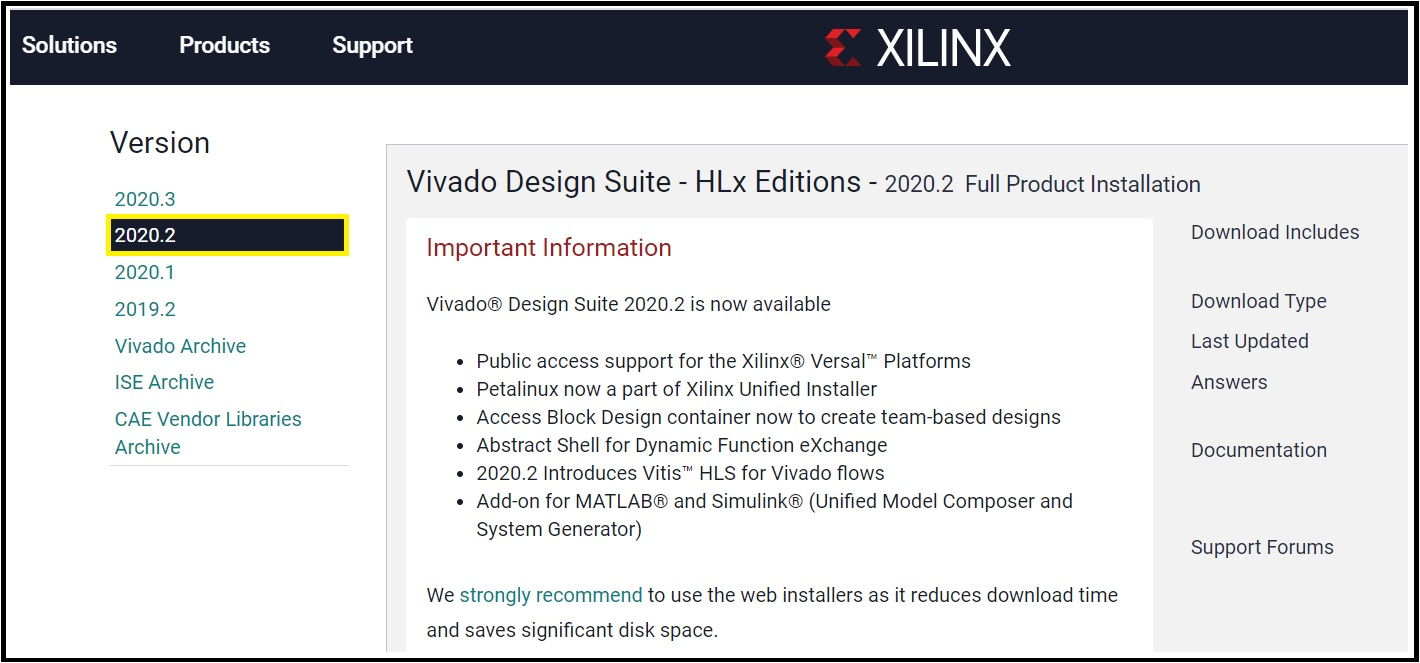
\includegraphics[width=\linewidth]{images/VivadoInstimg002.jpg}
  \end{center}
  Opmerking: sommige gebruikers hebben nog succes met oudere versies, omdat het hoofddoel hier is om een versie te installeren die de FPGA van uw doelhardware ondersteunt. \\
  \\
  Dat wil zeggen de Artix7 100T (voor Nexys en R2) of 200T (R3/R3A/R4).
\end{minipage}

\begin{minipage}{\linewidth}
  Klik op Xilinx Unified Installer 2020.2: Windows Self Extracting Web Installer EXE - 248.44MB
  \\
  \begin{center}
    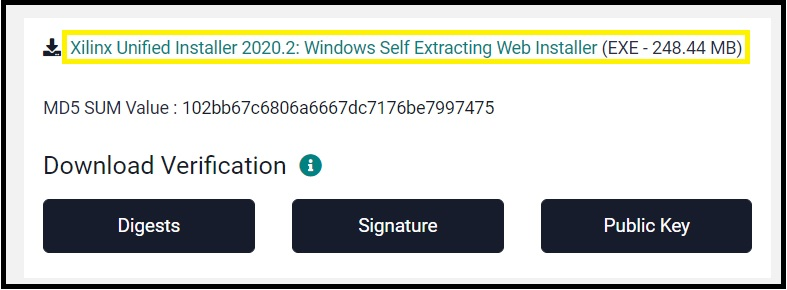
\includegraphics[width=0.8\linewidth]{images/VivadoInstimg003.jpg}
  \end{center}
\end{minipage}

\begin{minipage}{\linewidth}
  U wordt gevraagd een account aan te maken om in te kunnen loggen en het installatieprogramma te kunnen downloaden. \\
  \\
  Uw inloggegevens worden ook gevraagd tijdens de installatie.
  \\
  \begin{center}
    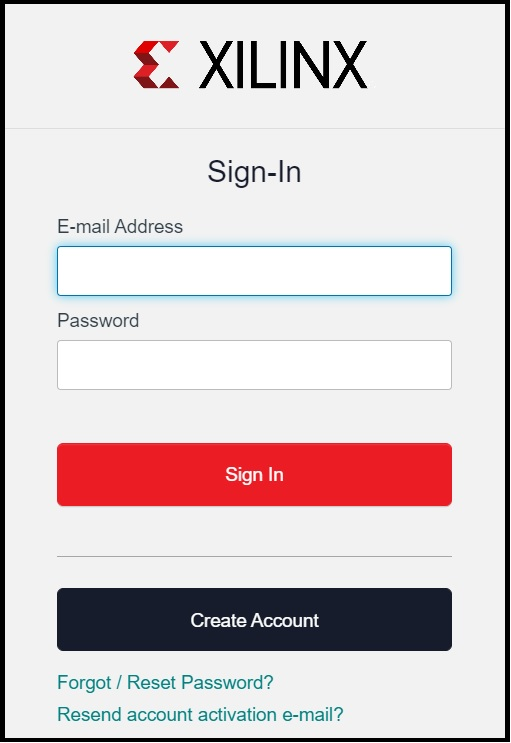
\includegraphics[width=0.3\linewidth]{images/VivadoInstimg004.jpg}
  \end{center}
\end{minipage}

\begin{minipage}{\linewidth}
  Nadat u ingelogd bent, moet u enkele persoonlijke gegevens invullen en dan op Download klikken.
  \\
  \begin{center}
    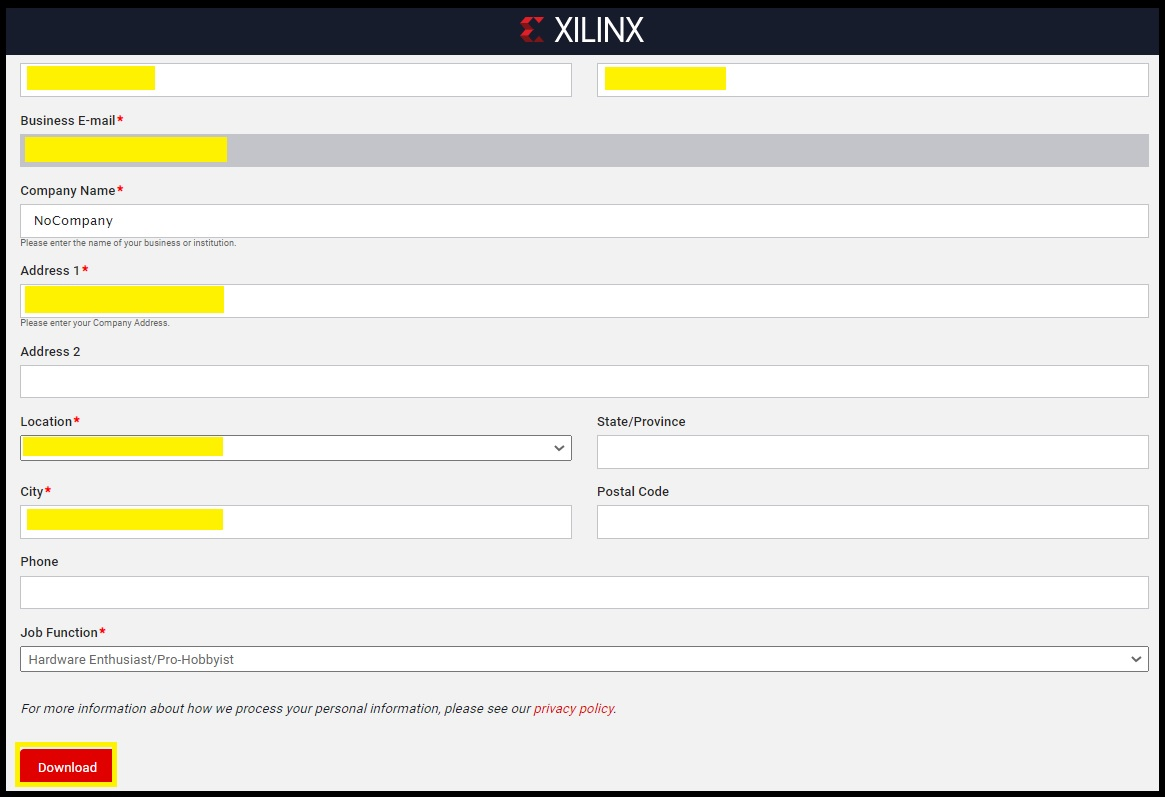
\includegraphics[width=0.8\linewidth]{images/VivadoInstimg005.jpg}
  \end{center}
\end{minipage}

\begin{minipage}{\linewidth}
  Voer het installatieprogramma uit als beheerder (Xilinx\_Unified\_2020.2\_1118\_1232\_Win64.exe).
  \\
  \begin{center}
    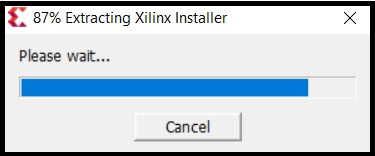
\includegraphics[width=0.5\linewidth]{images/VivadoInstimg006.jpg}
  \end{center}
\end{minipage}

\begin{minipage}{\linewidth}
  Klik op Allow Access.
  \\
  \begin{center}
    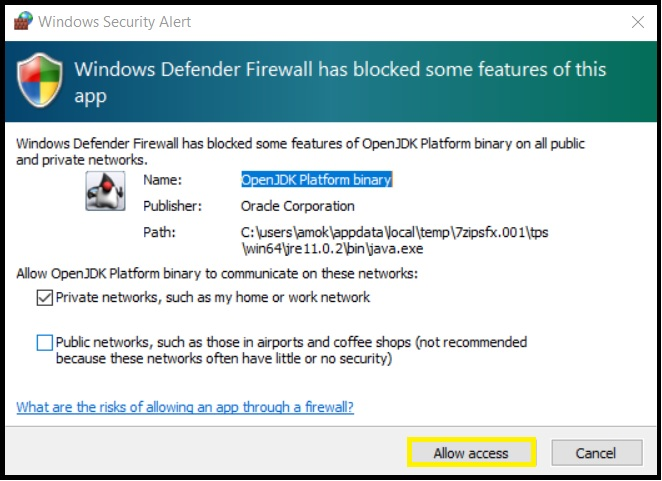
\includegraphics[width=0.5\linewidth]{images/VivadoInstimg007.jpg}
  \end{center}
\end{minipage}

\begin{minipage}{\linewidth}
  Klik op Next.
  \\
  \begin{center}
    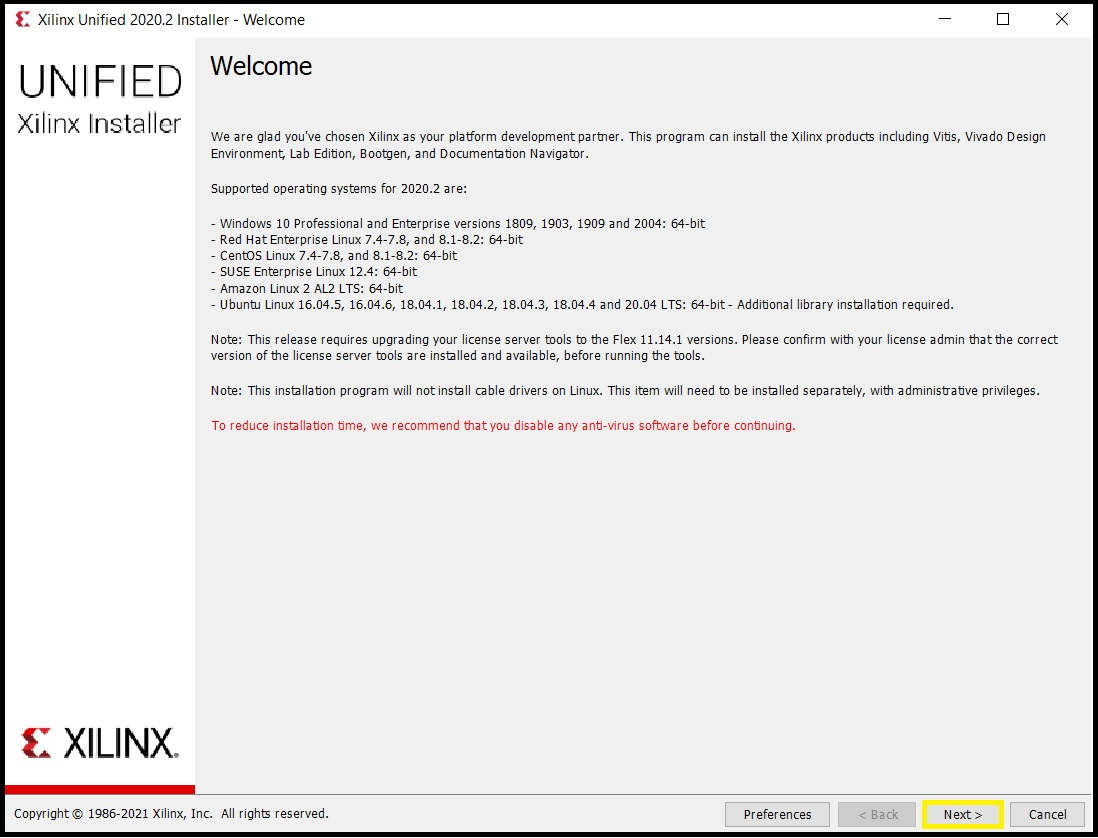
\includegraphics[width=0.7\linewidth]{images/VivadoInstimg008.jpg}
  \end{center}
\end{minipage}

\begin{minipage}{\linewidth}
  Voer uw inloggegevens in en klik op Next.
  \\
  \begin{center}
    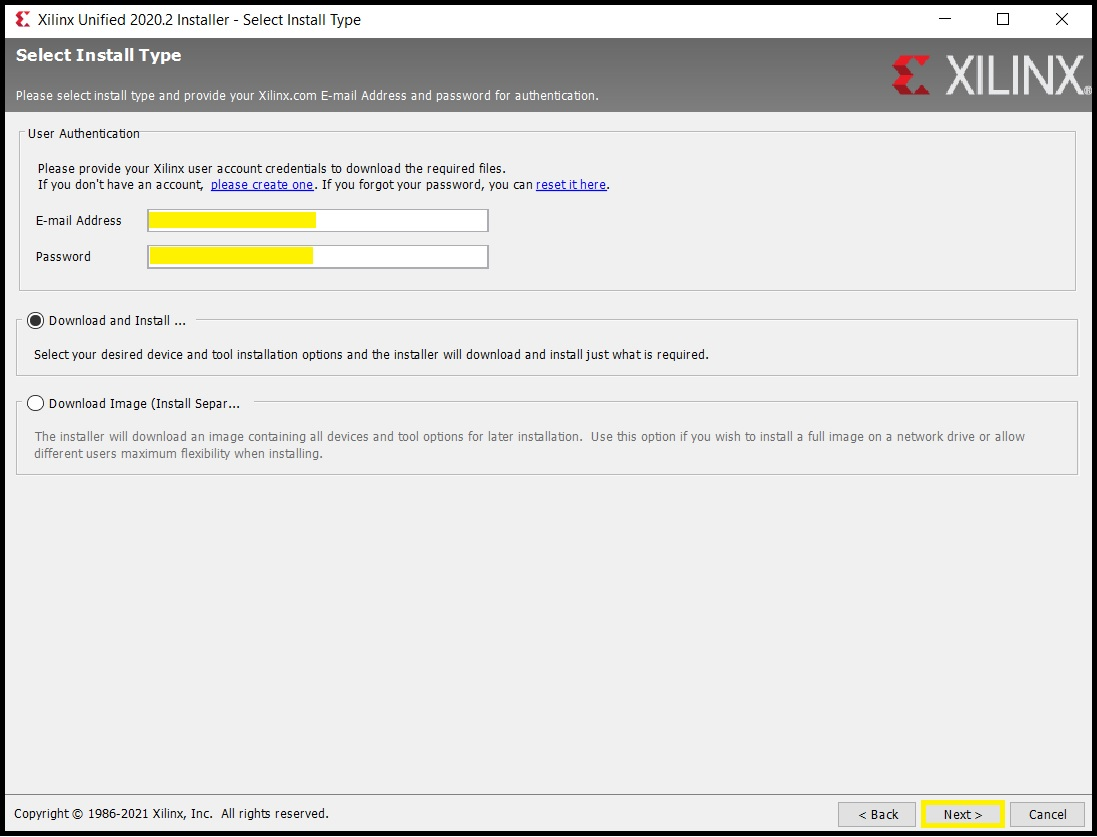
\includegraphics[width=0.7\linewidth]{images/VivadoInstimg009.jpg}
  \end{center}
\end{minipage}

\begin{minipage}{\linewidth}
  Selecteer Vivado en klik op Next.
  \\
  \begin{center}
    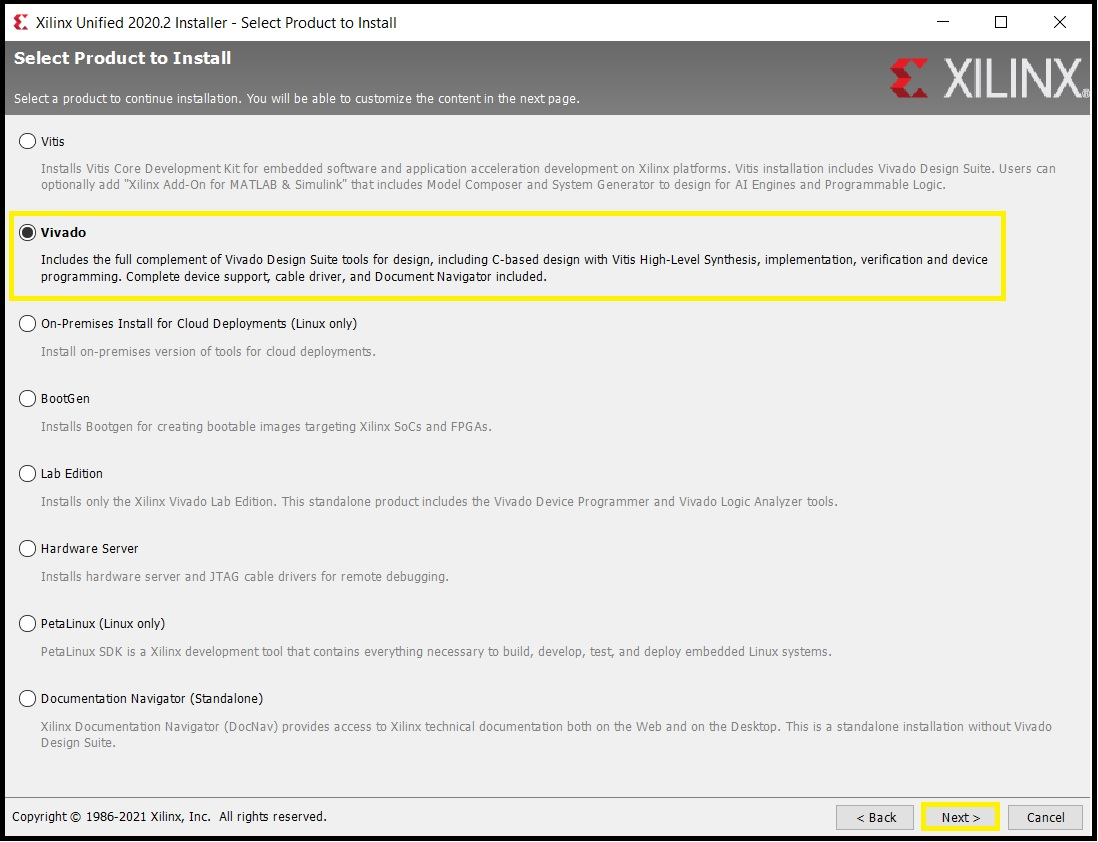
\includegraphics[width=0.7\linewidth]{images/VivadoInstimg010.jpg}
  \end{center}
\end{minipage}

\begin{minipage}{\linewidth}
  Selecteer ``Vivado HL WebPACK'' en klik op ``Next''.
  \\
  \begin{center}
    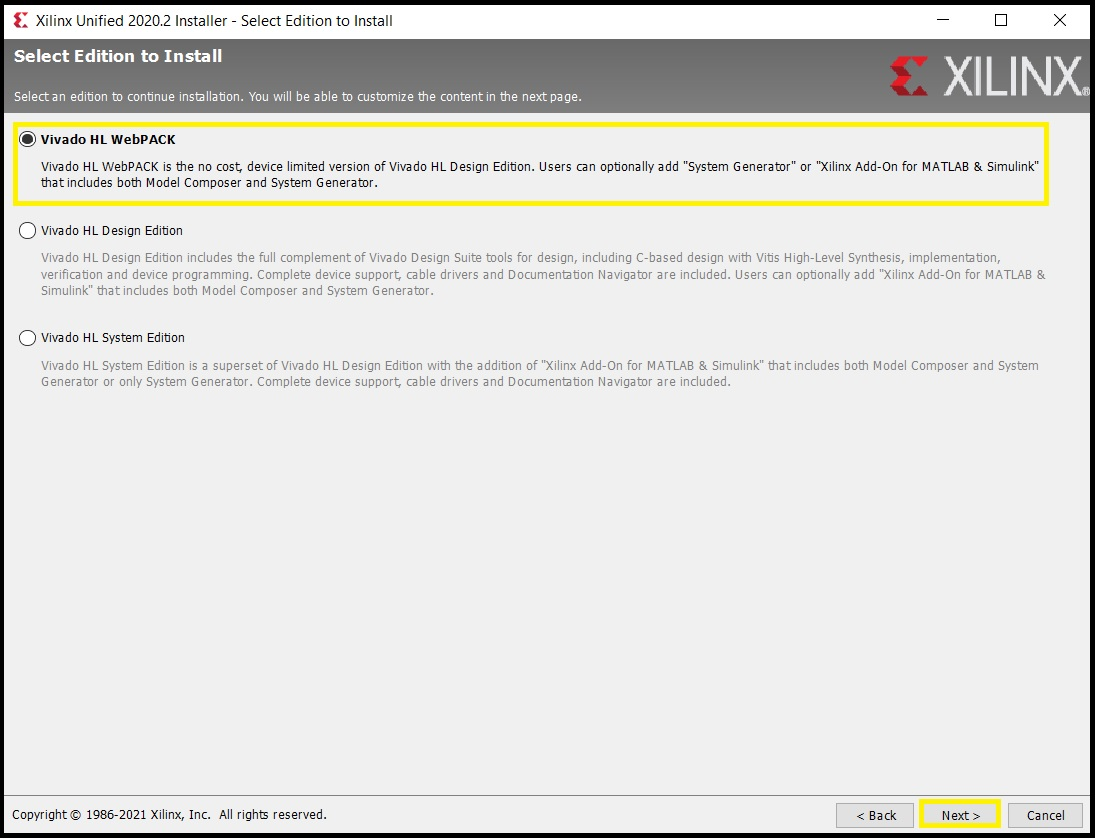
\includegraphics[width=0.7\linewidth]{images/VivadoInstimg011.jpg}
  \end{center}
\end{minipage}

\begin{minipage}{\linewidth}
  Wij raden aan om alleen de apparaten uit de ``\textbf{7 Series}'' te selecteren, omdat onze gekozen FPGA in deze serie valt, en het deselecteren van de andere series bespaart u ongeveer 6 GB aan downloadgrootte. Klik dan op ``Next''.
  \\
  \begin{center}
    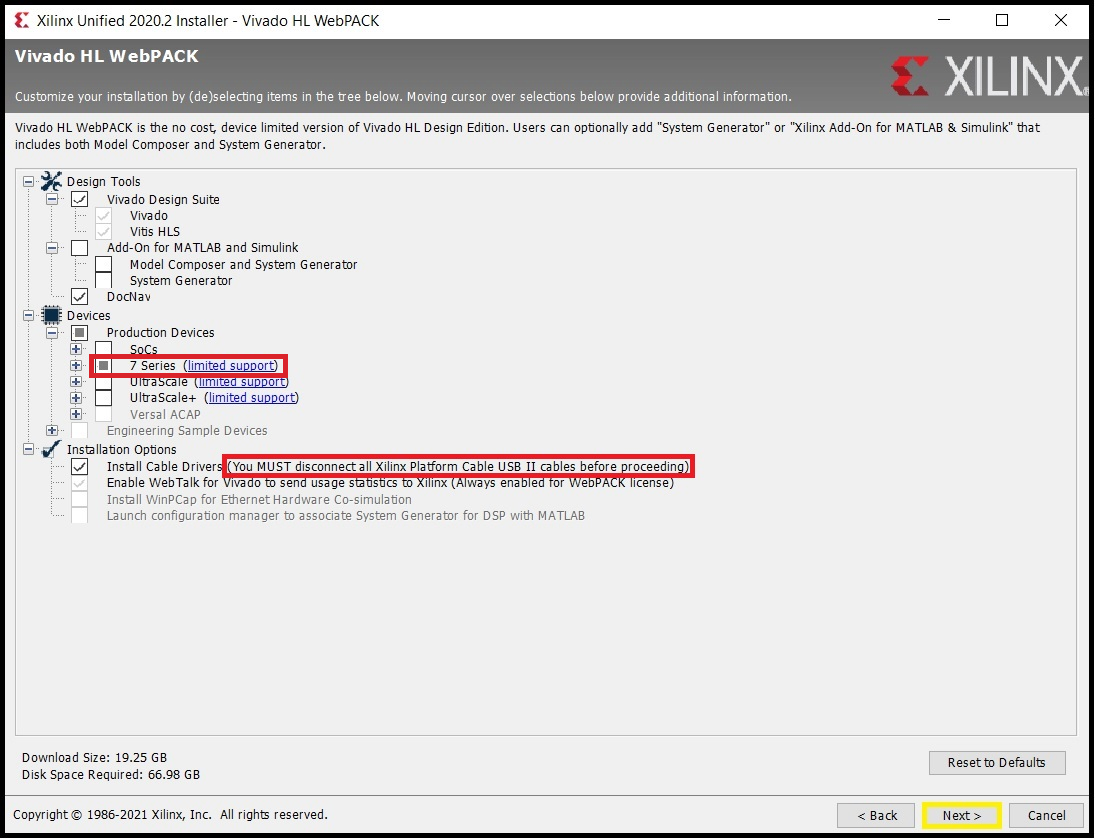
\includegraphics[width=0.7\linewidth]{images/VivadoInstimg012.png}
  \end{center}
  Waarschuwing: zoals gezegd, ontkoppel elke USB-kabel die op uw pc is aangesloten van het Nexys-bord.
\end{minipage}

\begin{minipage}{\linewidth}
  Ga akkoord met alle bepalingen van de eindgebruikerslicentieovereenkomst en de voorwaarden en klik op ``Next''.
  \\
  \begin{center}
    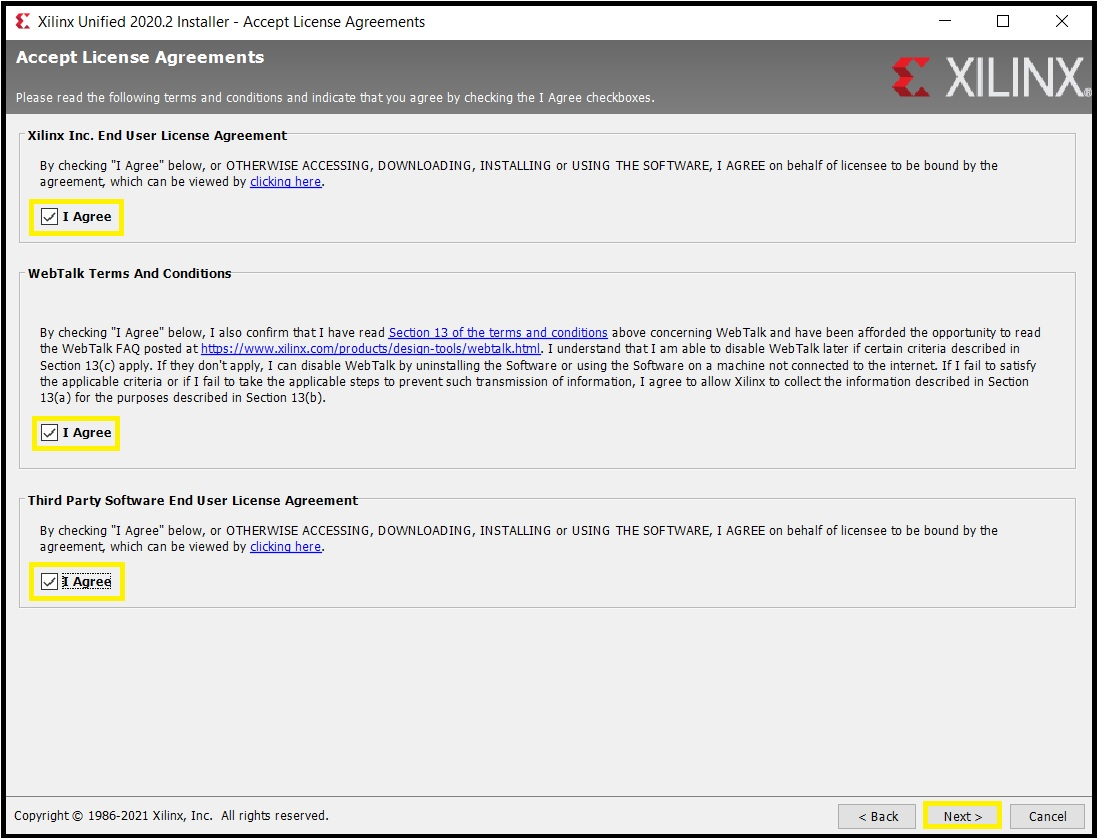
\includegraphics[width=0.7\linewidth]{images/VivadoInstimg013.jpg}
  \end{center}
\end{minipage}

\begin{minipage}{\linewidth}
  Kies de locatie waar u de software wilt installeren en klik op ``Next''.
  \\
  \begin{center}
    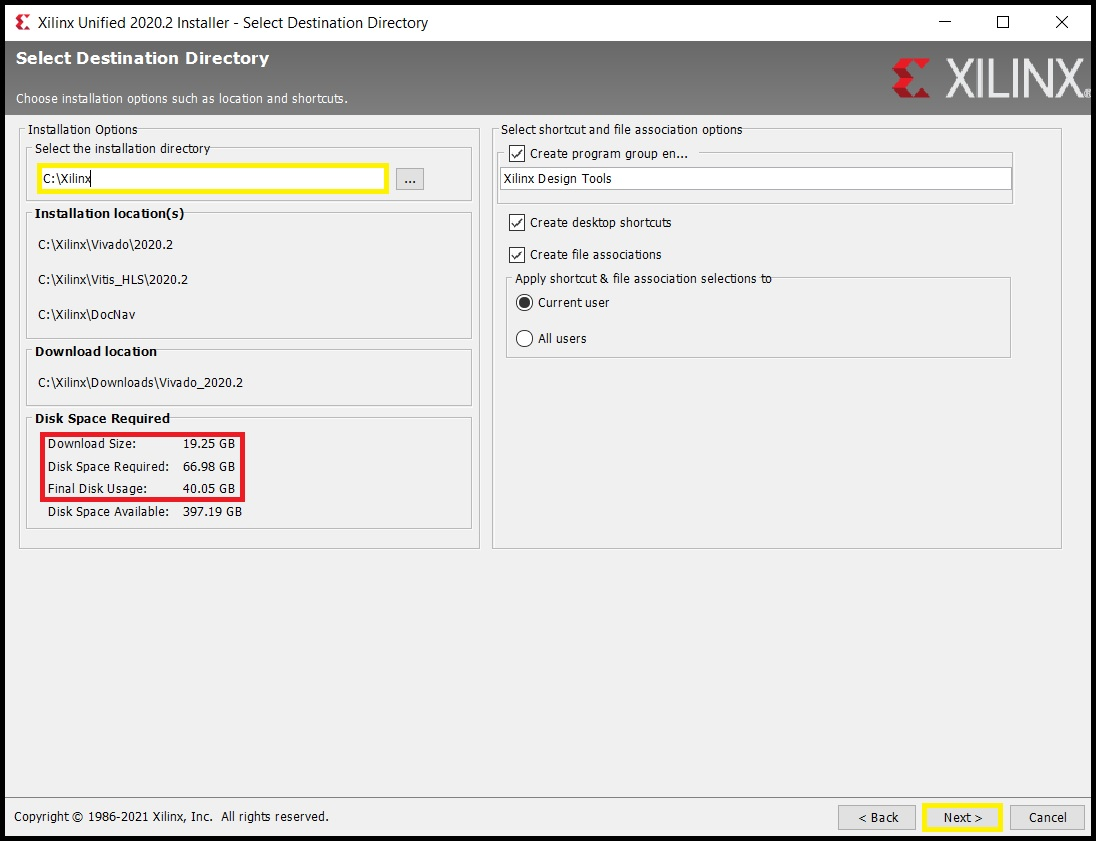
\includegraphics[width=0.7\linewidth]{images/VivadoInstimg014.jpg}
  \end{center}
  Waarschuwing: u staat op het punt om 20 GB aan software te downloaden en u hebt 70 GB nodig om de installatie uit te voeren.
\end{minipage}

\begin{minipage}{\linewidth}
  Klik op ``Yes''.
  \\
  \begin{center}
    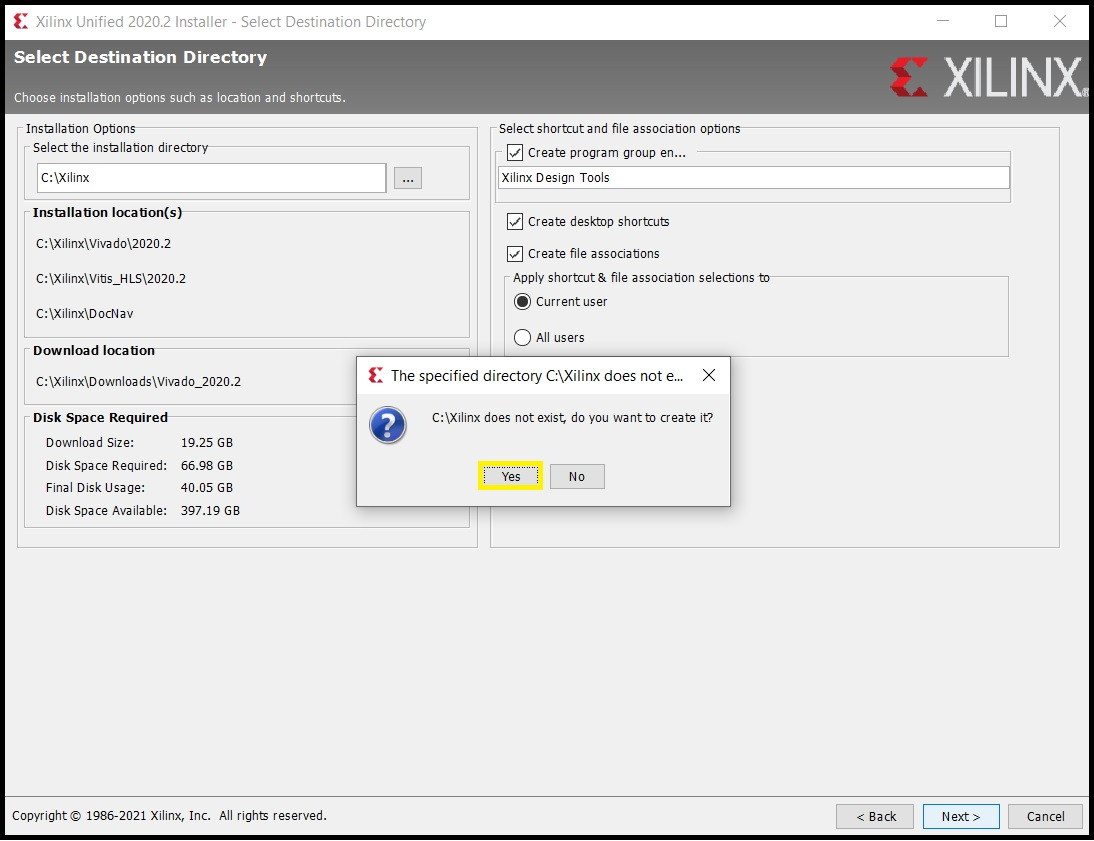
\includegraphics[width=0.7\linewidth]{images/VivadoInstimg015.jpg}
  \end{center}
\end{minipage}

\begin{minipage}{\linewidth}
  Klik op ``Install''.
  \\
  \begin{center}
    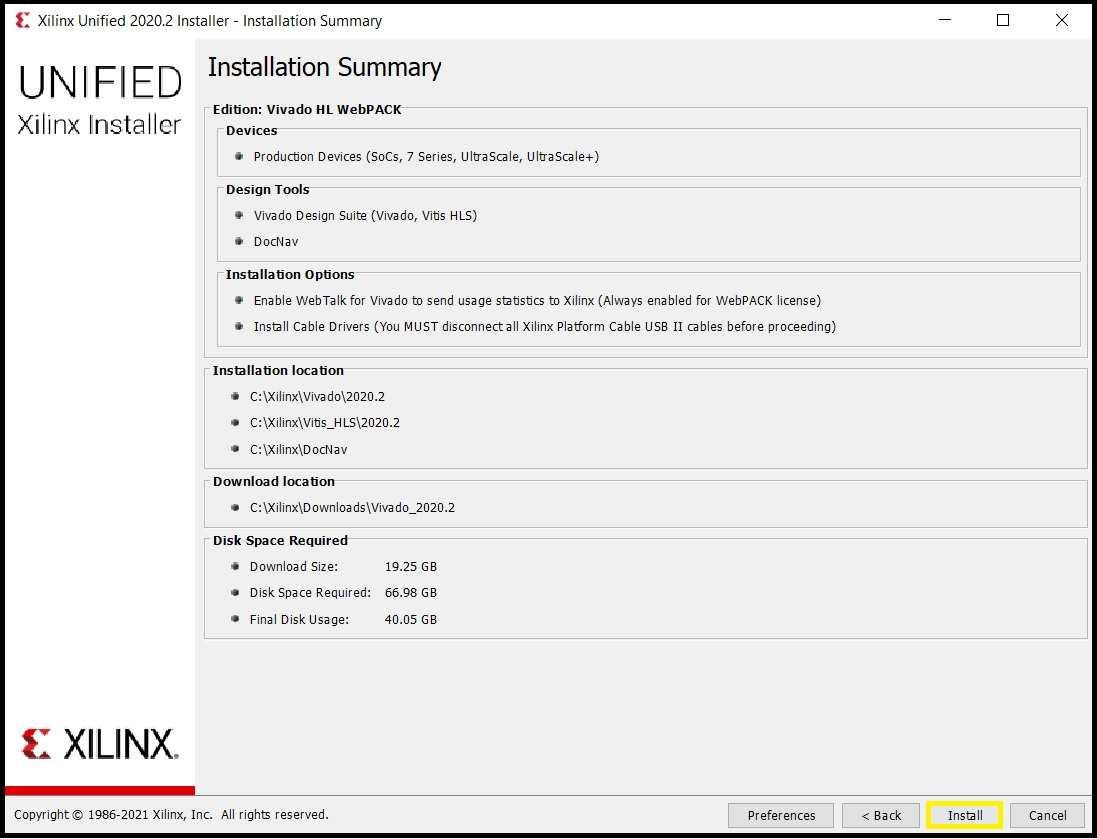
\includegraphics[width=0.7\linewidth]{images/VivadoInstimg016.jpg}
  \end{center}
\end{minipage}

\begin{minipage}{\linewidth}
  Wacht tot de installatie is voltooid. Aan het einde van de installatie wordt u gevraagd of u de Xilinx-apparatensoftware wilt installeren.
  \\
  \begin{center}
    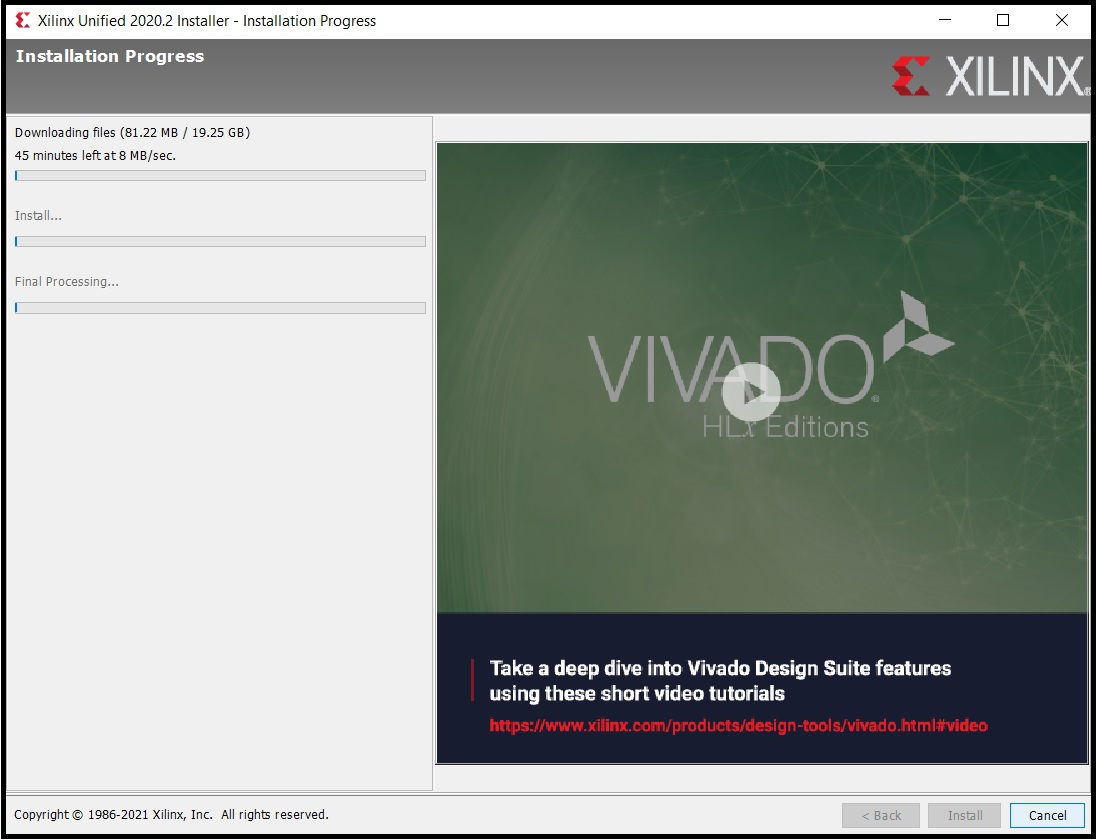
\includegraphics[width=0.7\linewidth]{images/VivadoInstimg017.jpg}
  \end{center}
\end{minipage}

\begin{minipage}{\linewidth}
  Klik op ``Install''.
  \\
  \begin{center}
    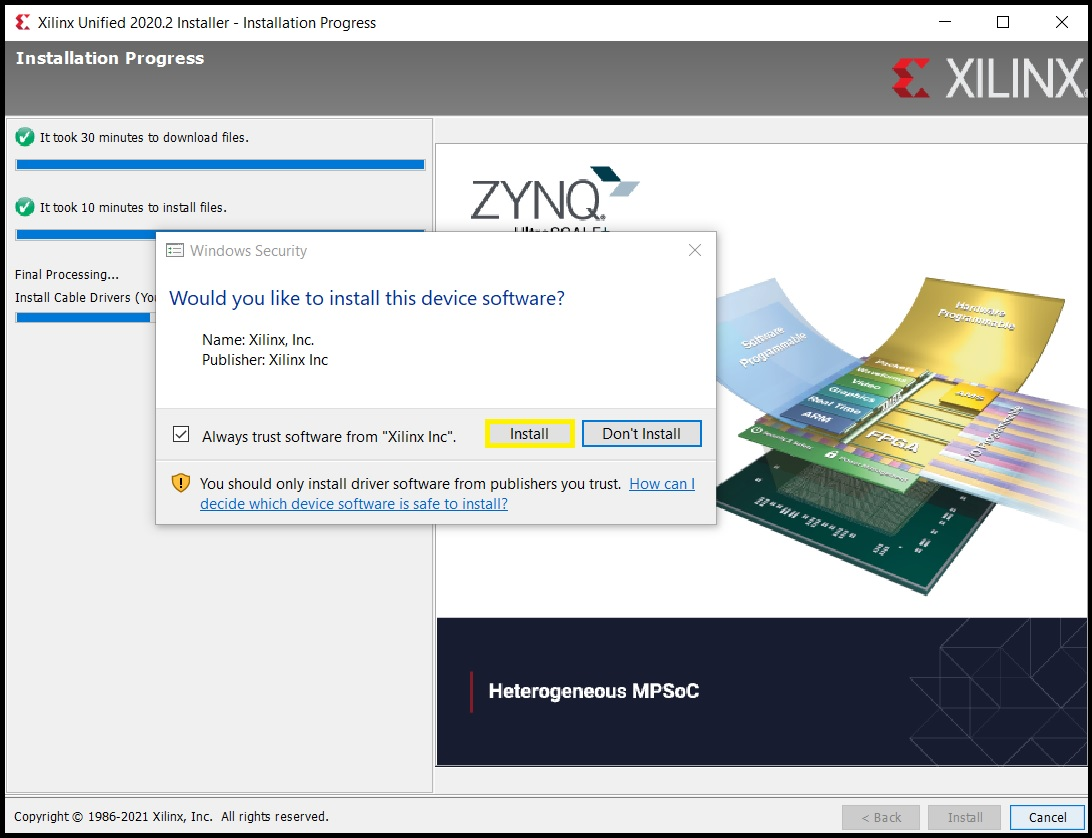
\includegraphics[width=0.7\linewidth]{images/VivadoInstimg018.jpg}
  \end{center}
  Laat de installatie voltooien.
\end{minipage}

\begin{minipage}{\linewidth}
  De installatie is voltooid. Klik op ``OK''.
  \\
  \begin{center}
    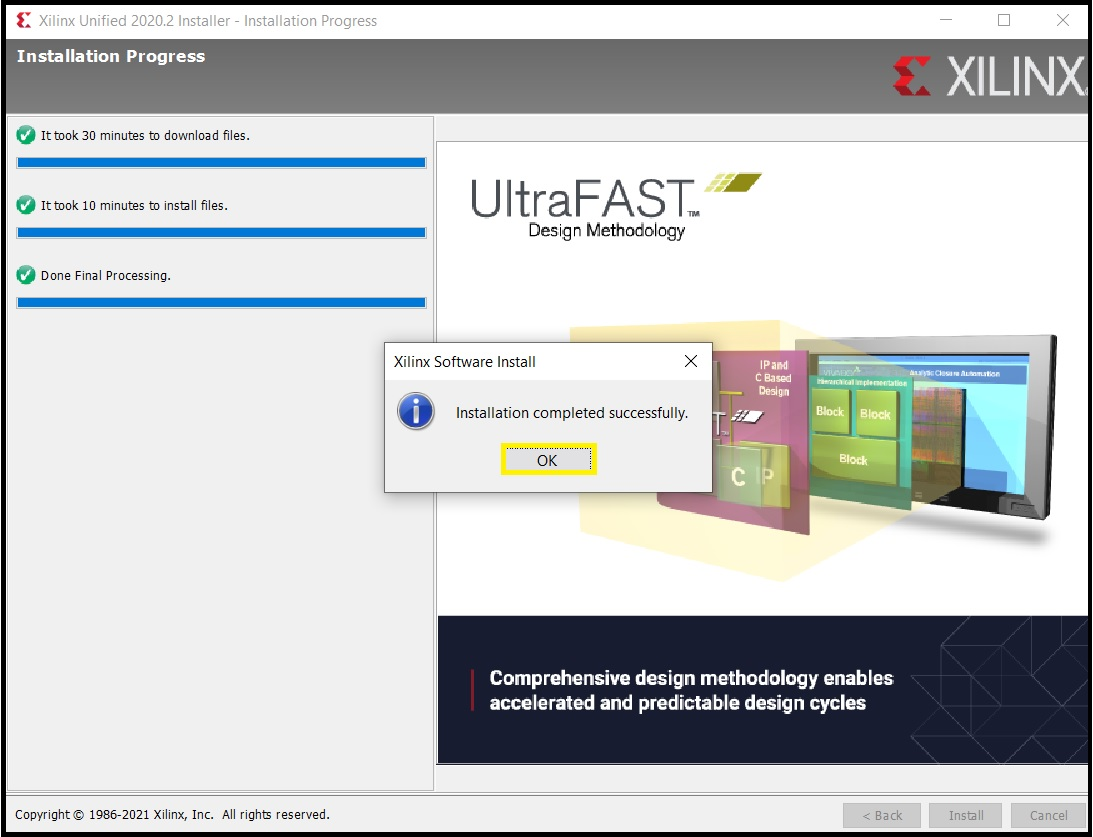
\includegraphics[width=0.7\linewidth]{images/VivadoInstimg019.jpg}
  \end{center}
\end{minipage}

\begin{minipage}{\linewidth}
  Op uw bureaublad verschijnen nu de volgende pictogrammen:
  \\
  \begin{center}
    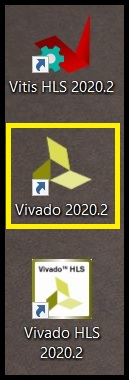
\includegraphics[width=0.2\linewidth]{images/VivadoInstimg020.jpg}
  \end{center}
  Let op: Ubuntu-gebruikers moeten mogelijk een ontbrekende afhankelijkheid installeren met: {\tt sudo apt install libtinfo5}
\end{minipage}

\begin{minipage}{\linewidth}
  Start Vivado 2020.2
  \\
  \begin{center}
    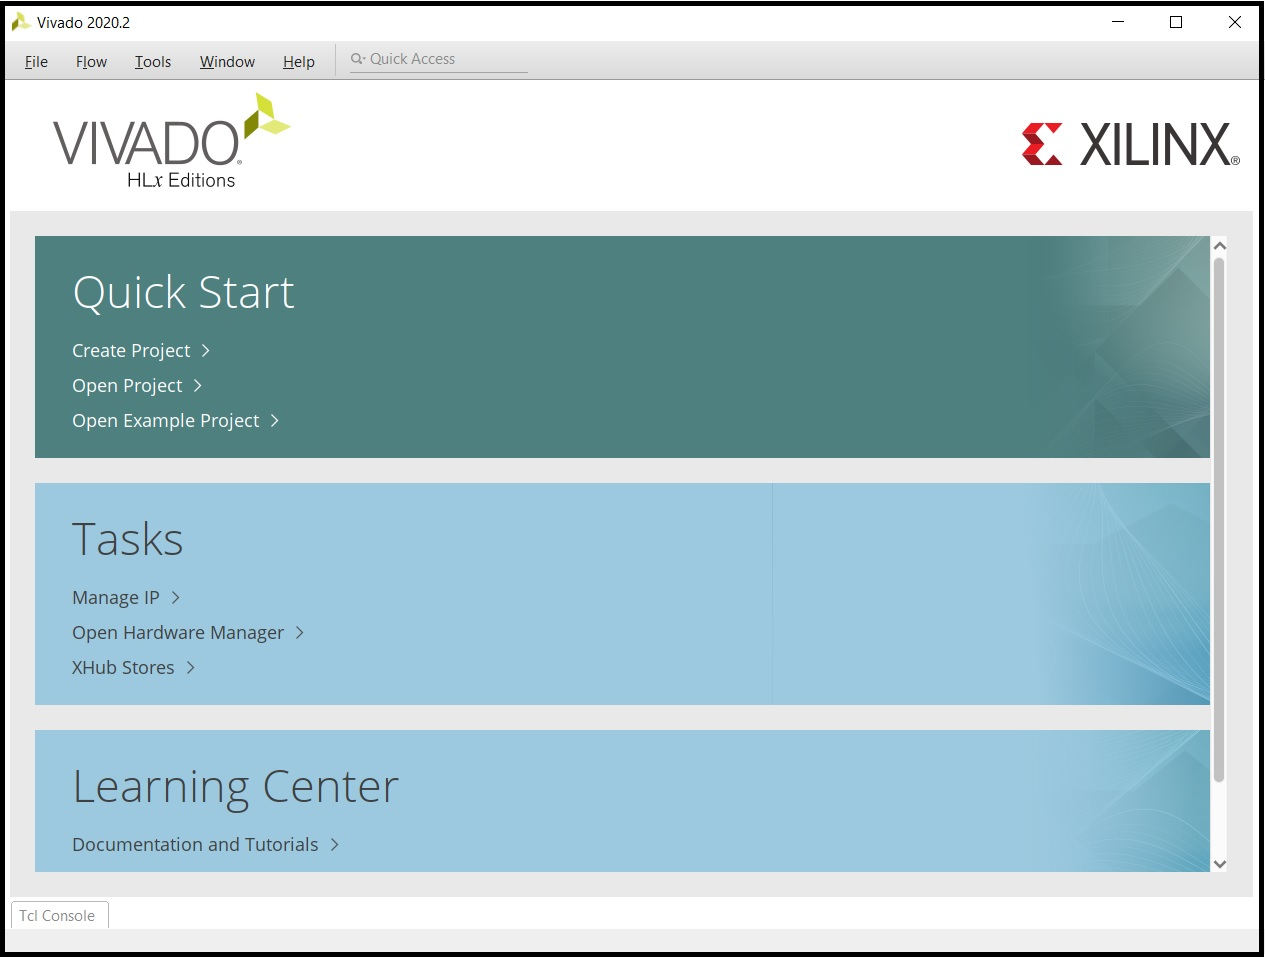
\includegraphics[width=0.7\linewidth]{images/VivadoInstimg021.jpg}
  \end{center}
\end{minipage}

\begin{minipage}{\linewidth}
  Klik op ``Help''->``Obtain a licence Key''.
  \\
  \begin{center}
    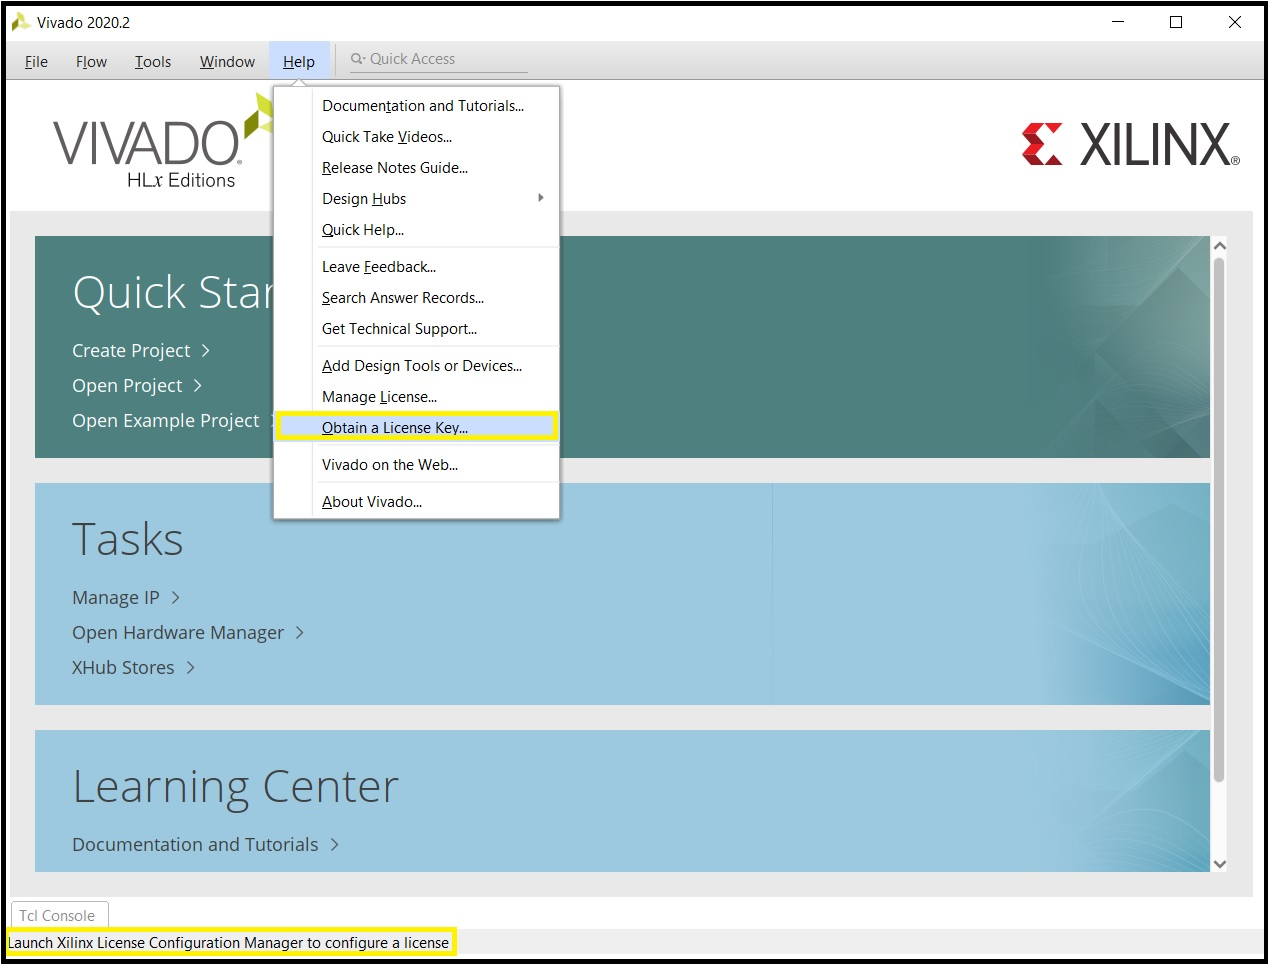
\includegraphics[width=0.7\linewidth]{images/VivadoInstimg022.jpg}
  \end{center}
\end{minipage}

\begin{minipage}{\linewidth}
  Hiermee opent u de Vivado-licentiemanager. \\
  \\
  Selecteer ``Get Free ISE WebPACK, ISE/Vivado IP or PetaLinux Licenses'' \\
  \\
  Klik op ``Connect Now''.
  \\
  \begin{center}
    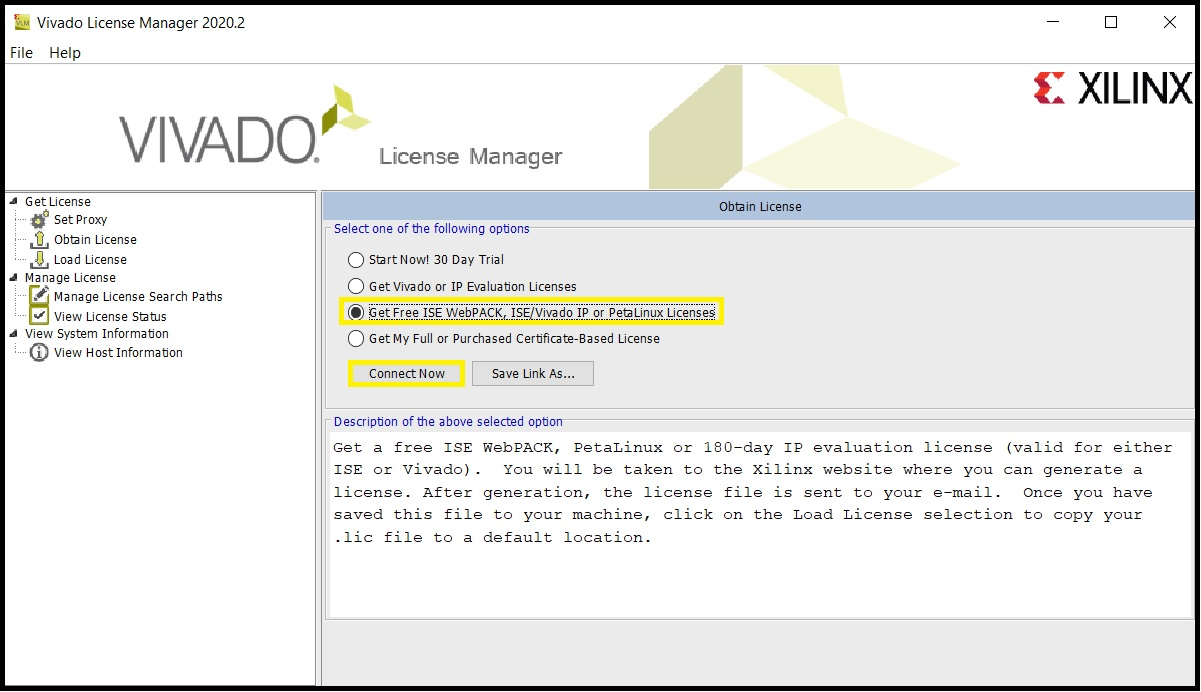
\includegraphics[width=\linewidth]{images/VivadoInstimg023.jpg}
  \end{center}
\end{minipage}

\begin{minipage}{\linewidth}
  Verbind met het gebruikersaccount dat u hebt aangemaakt om de Vivado-software te kunnen downloaden. Als u nog niet op de website van Xilinx was ingelogd, wordt u naar de hoofdpagina geleid. Keer terug naar de licentiemanager (die niet is gesloten).
  \\
  \begin{center}
    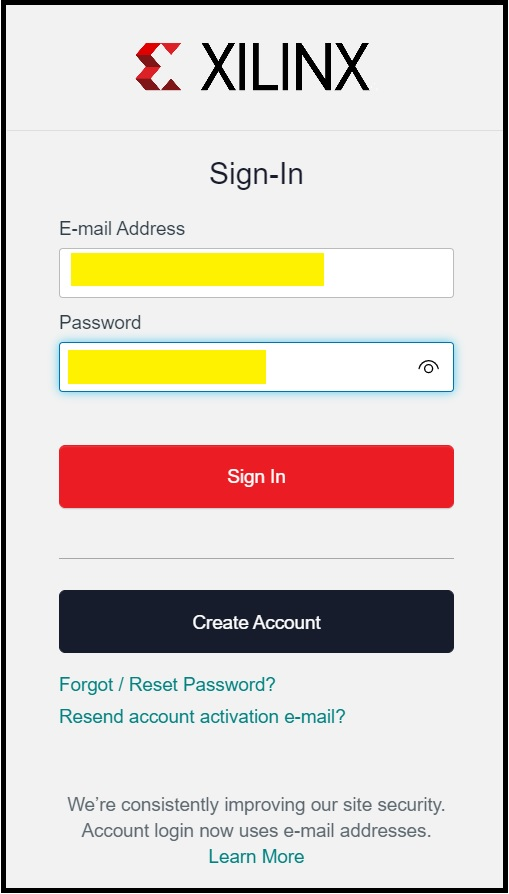
\includegraphics[width=0.3\linewidth]{images/VivadoInstimg024.jpg}
  \end{center}
\end{minipage}

\begin{minipage}{\linewidth}
  Klik opnieuw op ``Connect Now'' (controleer of ``Get Free ISE WebPACK, ISE/Vivado IP or PetaLinux Licenses'' nog steeds is geselecteerd).
  \\
  \begin{center}
    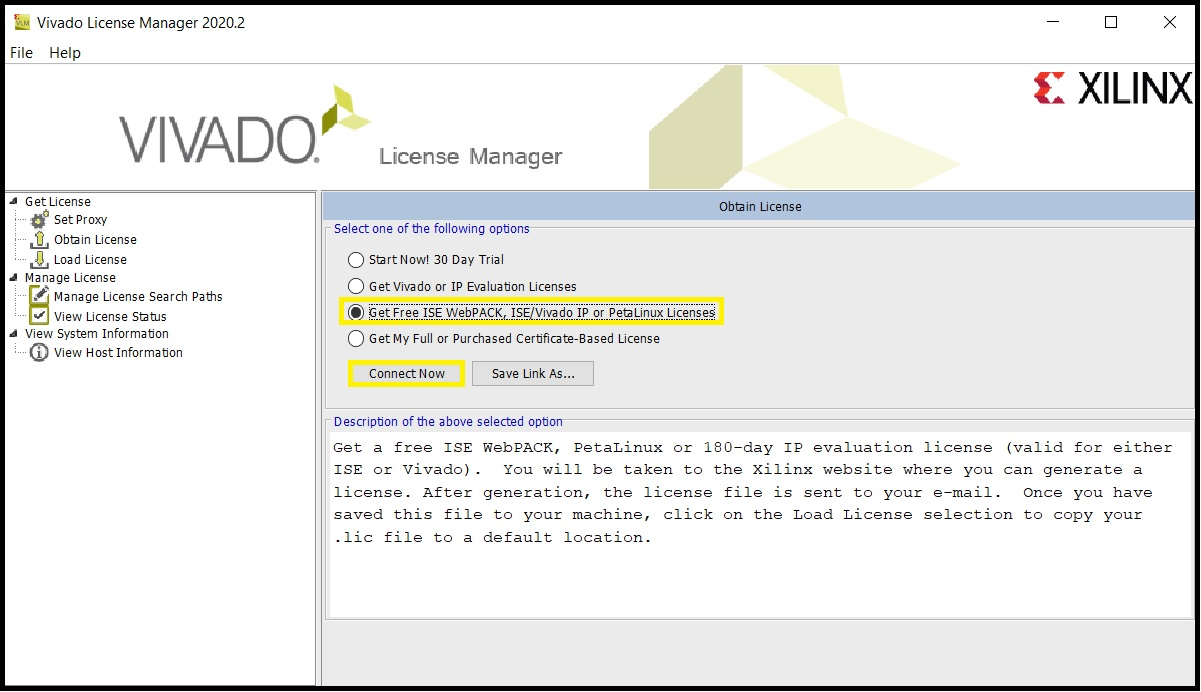
\includegraphics[width=\linewidth]{images/VivadoInstimg023.jpg}
  \end{center}
\end{minipage}

\begin{minipage}{\linewidth}
  Vervolgens registreert u uw persoonlijke gegevens op de Vivado-website en klikt u op ``Next''.
  \\
  \begin{center}
    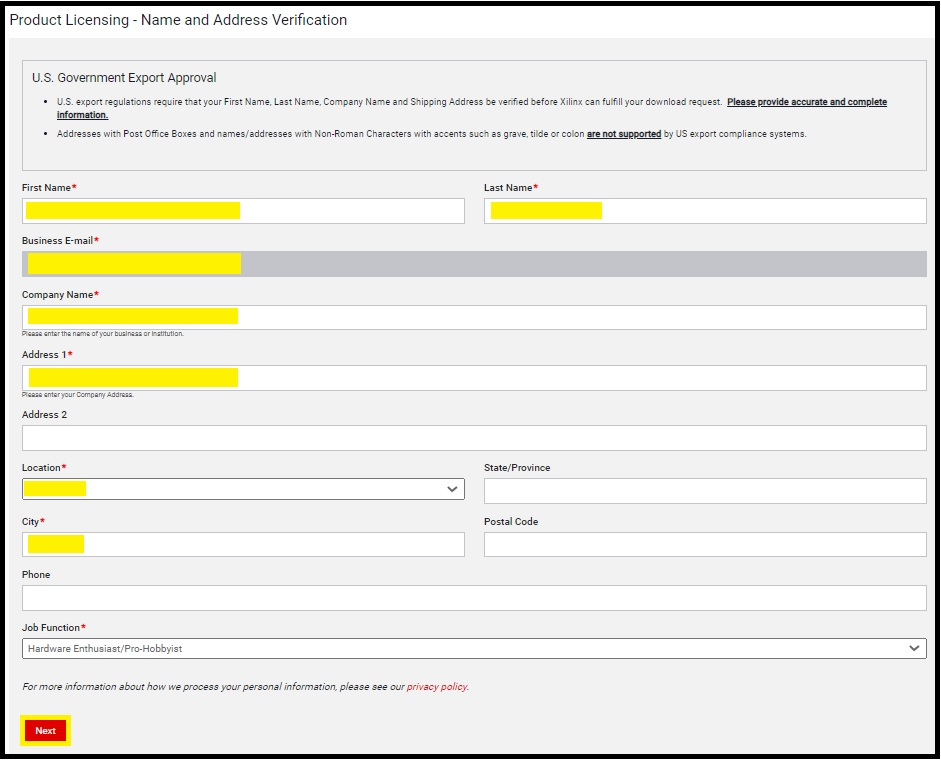
\includegraphics[width=0.7\linewidth]{images/VivadoInstimg025.jpg}
  \end{center}
\end{minipage}


\begin{minipage}{\linewidth}
Selecteer ``ISE WebPACK Licence'' en ``Vivado Design Suite: HL WebPACK 2015 and Earlier License'' \\
\\
Klik vervolgens op ``Generate Node-Locked Licence''.
\\
\begin{center}
  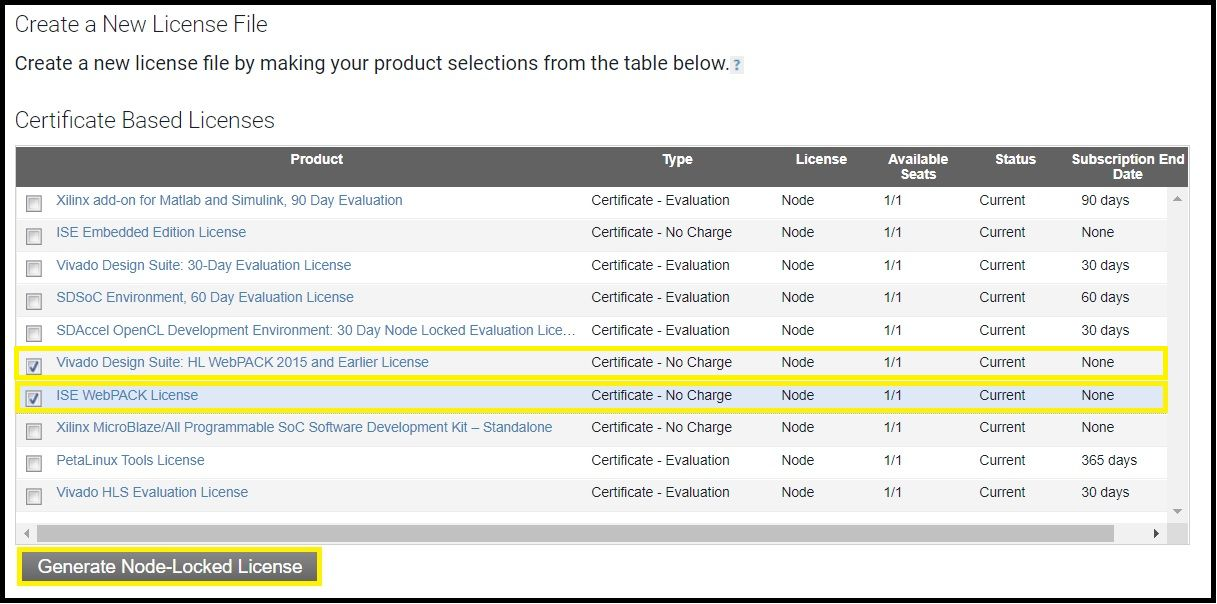
\includegraphics[width=\linewidth]{images/VivadoInstimg026.jpg}
\end{center}
\end{minipage}

\begin{minipage}{\linewidth}
  Klik op ``Next''.
  \\
  \begin{center}
    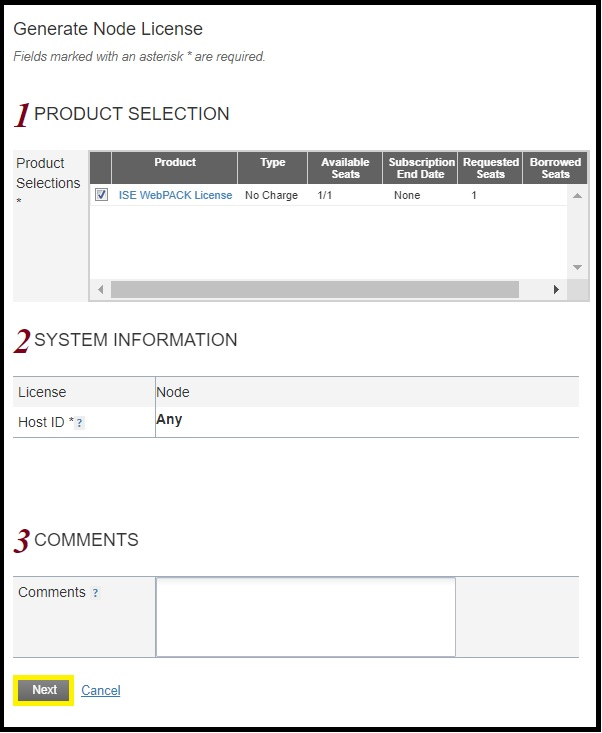
\includegraphics[width=0.5\linewidth]{images/VivadoInstimg027.jpg}
  \end{center}
\end{minipage}

\begin{minipage}{\linewidth}
  Klik op ``Next''.
  \\
  \begin{center}
    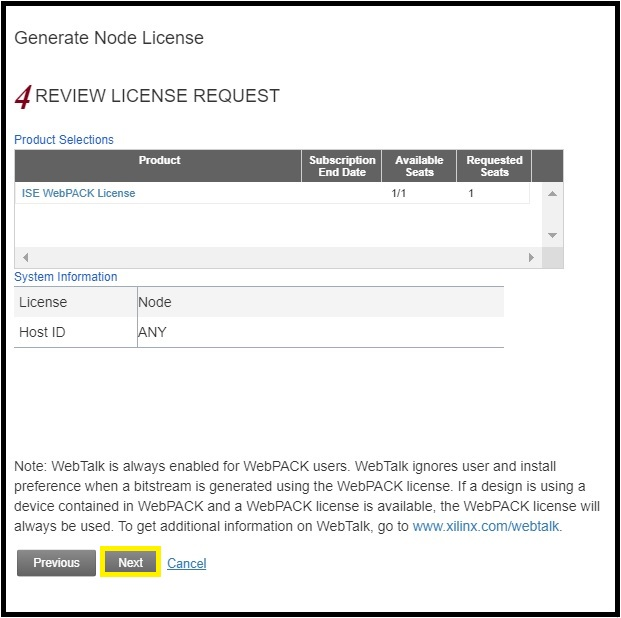
\includegraphics[width=0.5\linewidth]{images/VivadoInstimg028.jpg}
  \end{center}
\end{minipage}


\begin{minipage}{\linewidth}
  Controleer uw e-mail: u hebt een e-mail ontvangen van Xilinx, Inc. met een licentiebestand met de naam ``Xilinc.lic'' als bijlage. \\
  \\
  Sla dit bestand op uw computer op en bewaar het op een veilige plaats.
  \\
  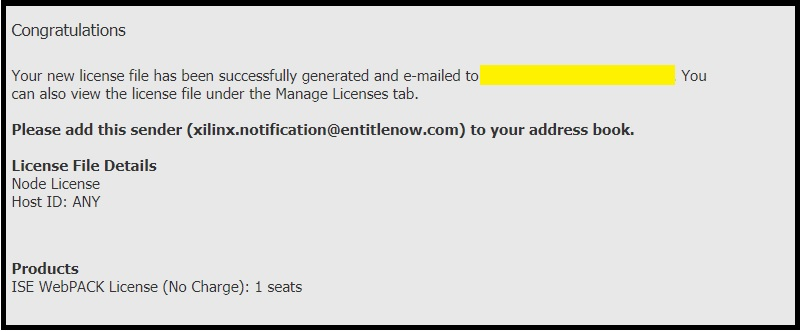
\includegraphics[width=\linewidth]{images/VivadoInstimg029.jpg}
\end{minipage}

\begin{minipage}{\linewidth}
  Ga terug naar de licentiemanager (die nog steeds actief is). \\
  \\
  Selecteer ``Load License'' en klik op ``Copy License''.
  \\
  \begin{center}
    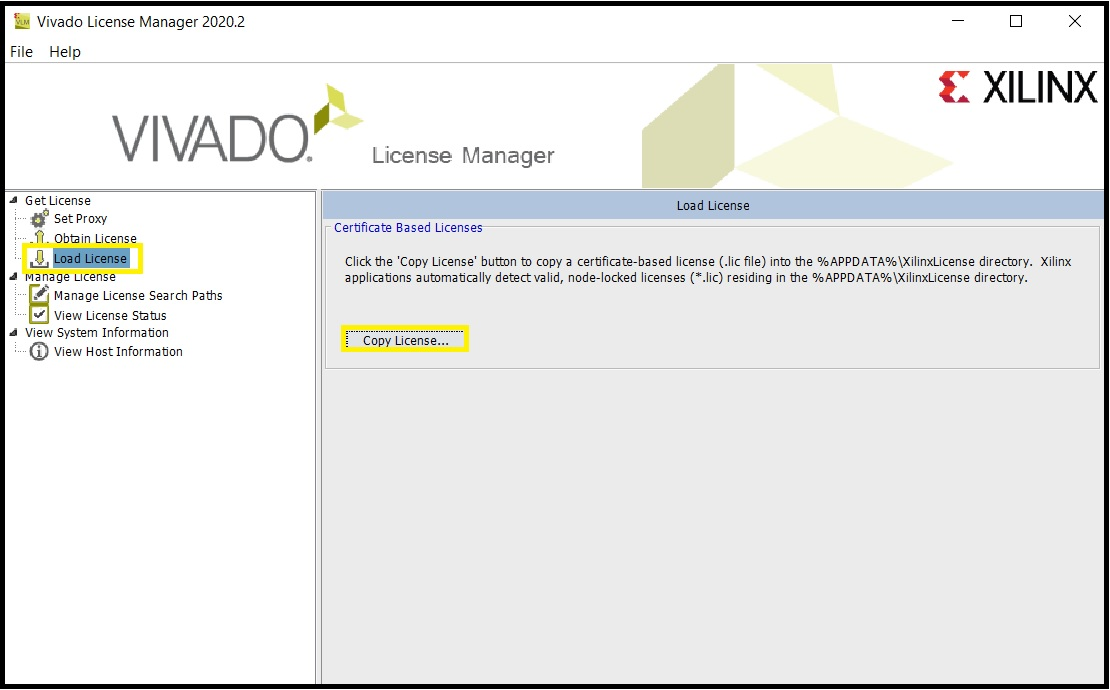
\includegraphics[width=0.8\linewidth]{images/VivadoInstimg030.jpg}
  \end{center}
\end{minipage}

\begin{minipage}{\linewidth}
  Blader naar de locatie waar u het bestand ``Xilinc.lic'' heeft opgeslagen, selecteer het en klik op ``Open''.
  \\
  \begin{center}
    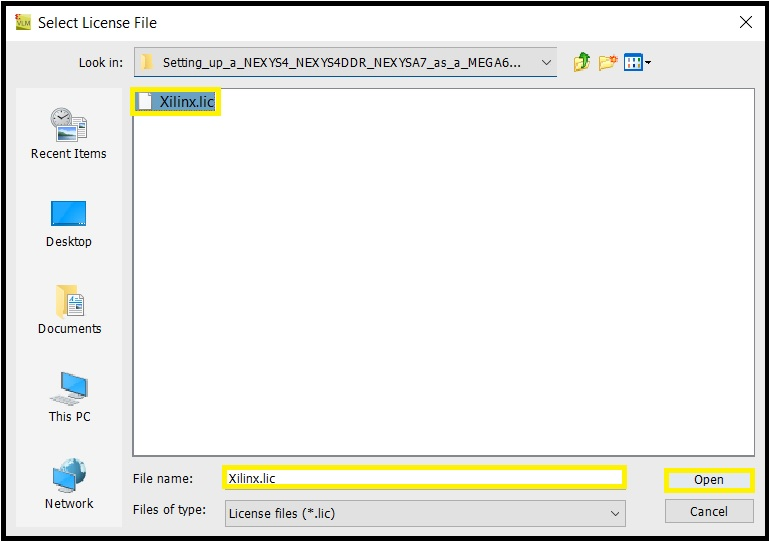
\includegraphics[width=0.7\linewidth]{images/VivadoInstimg031.jpg}
  \end{center}
\end{minipage}

\begin{minipage}{\linewidth}
  Klik op ``OK'' en sluit de Vivado-licentiemanager.
  \\
  \begin{center}
    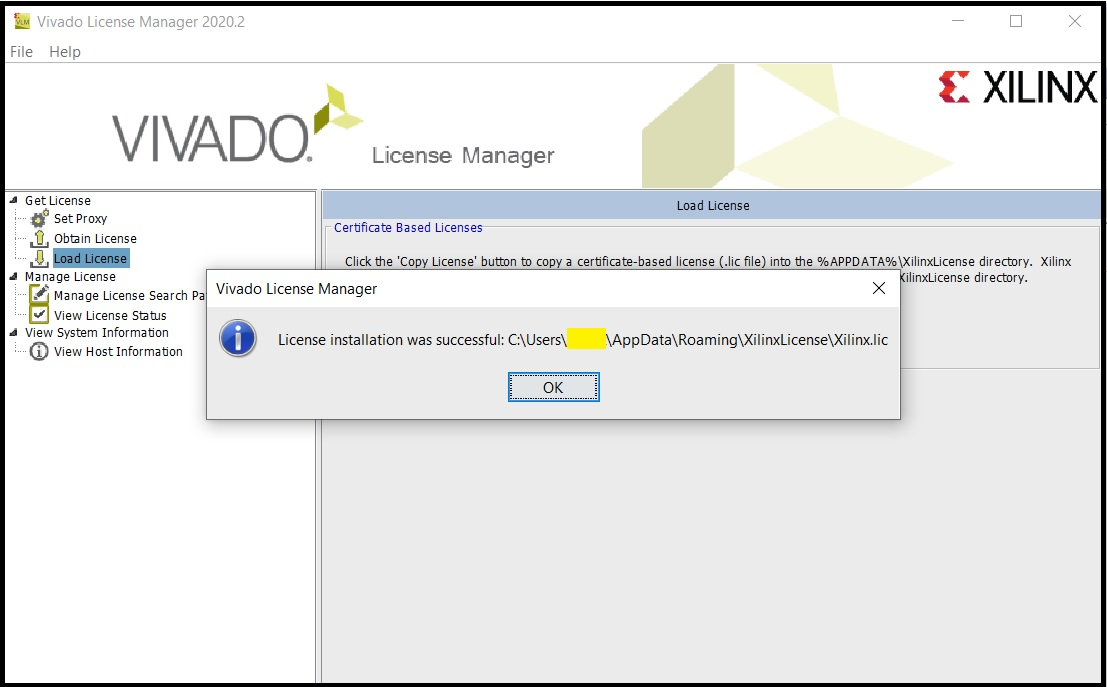
\includegraphics[width=0.7\linewidth]{images/VivadoInstimg032.jpg}
  \end{center}

  Uw Vivado-software is geregistreerd en u kunt deze nu gebruiken.
\end{minipage}

\section{De FTDI-stuurprogramma's installeren}

De FTDI-drivers zijn nodig om uw PC te laten communiceren met de JTAG-poort en de seriële communicatiepoort van de hardware (merk op dat de enkele fysieke USB-verbinding met uw PC feitelijk deze twee poorten aanbiedt).

\subsection{Linux-drivers}

Gebruikers van Linux melden dat zij de FTDI-drivers standaard in hun Linux-distributie aangetroffen hebben, terwijl anderen aangeven dat het volgende extra commando na de installatie van Vivado uitgevoerd moet worden:

cd /opt/Xilinx/Vivado/2018.3/data/xicom/cable\_drivers/lin64/install\_script/install\_drivers \\sudo ./install\_drivers

\subsection{Windows-drivers}

Download het volgende archief om de drivers te installeren:

\begin{itemize}
  \item \url{https://ftdichip.com/wp-content/uploads/2021/08/CDM212364_Setup.zip}
\end{itemize}

Pak het bestand \textbf{CDM212364\_Setup.zip} uit; u verkrijgt het bestand \textbf{CDM212364\_Setup.exe}.

\textcolor{red}{\underline{Waarschuwing}: \\Voordat u de drivers installeert, moet u de Nexys4-plaat uitschakelen en de USB-kabel loskoppelen van de PC.}

\begin{minipage}{\linewidth}
  Controleer welke apparaten er voor de installatie al aanwezig zijn:
  \\
  \begin{center}
    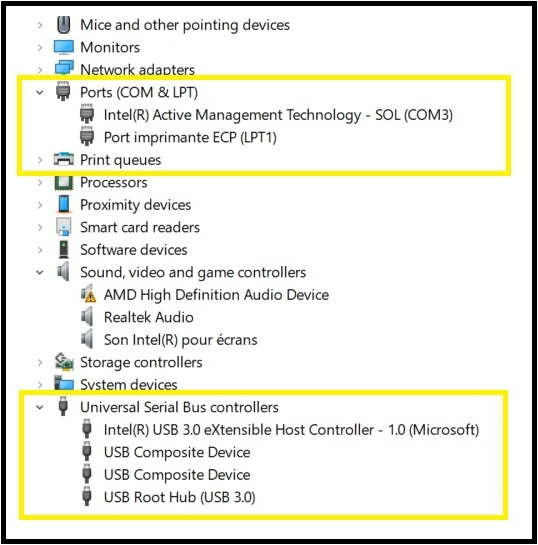
\includegraphics[width=0.6\linewidth]{images/img001_install_drivers_00.jpg}
  \end{center}
\end{minipage}

\begin{minipage}{\linewidth}
  Voer het bestand CDM212364\_Setup.exe uit als administrator:
  \\
  \begin{center}
    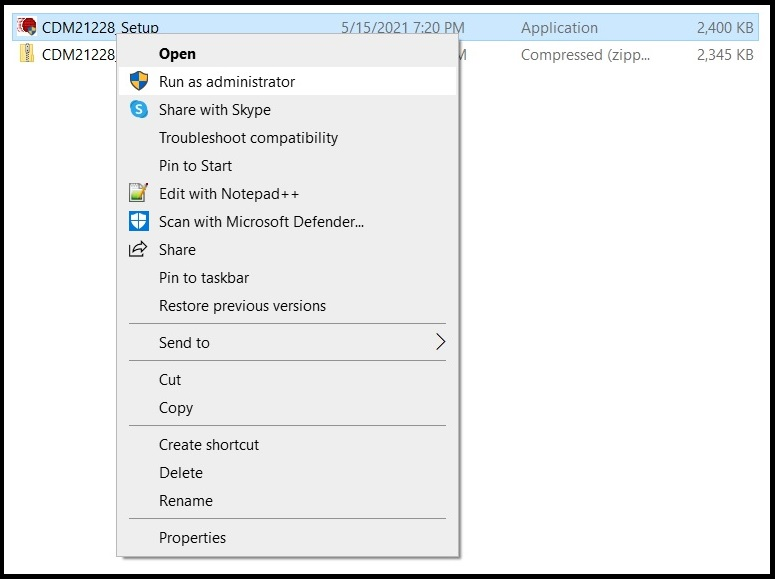
\includegraphics[width=0.6\linewidth]{images/img001_install_drivers_01.jpg}
  \end{center}
\end{minipage}

Bevestig dat u het programma wilt uitvoeren.

\begin{minipage}{\linewidth}
  Klik op ``Extract''.
  \\
  \begin{center}
    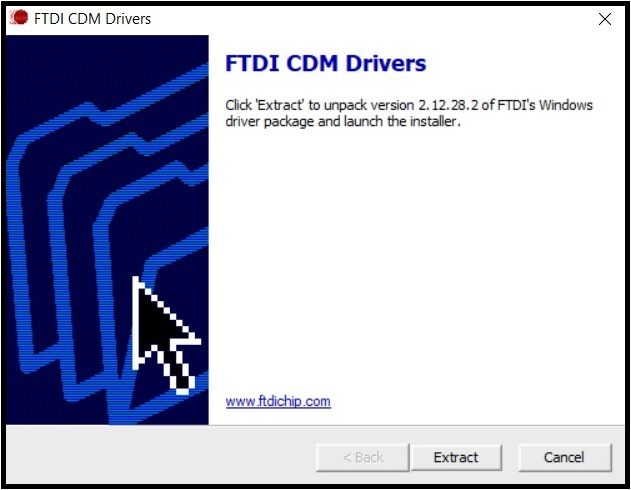
\includegraphics[width=0.6\linewidth]{images/img001_install_drivers_02.jpg}
  \end{center}
\end{minipage}

\begin{minipage}{\linewidth}
  Klik op ``Next >''.
  \\
  \begin{center}
    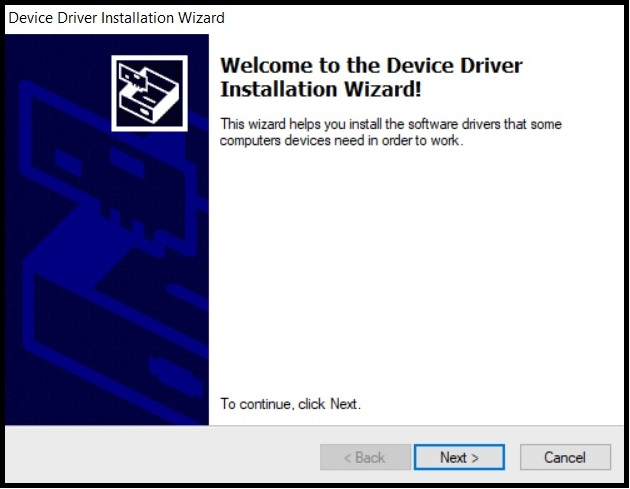
\includegraphics[width=0.6\linewidth]{images/img001_install_drivers_03.jpg}
  \end{center}
\end{minipage}

\begin{minipage}{\linewidth}
  Aanvaard de overeenkomst en klik op ``Next >''.
  \\
  \begin{center}
    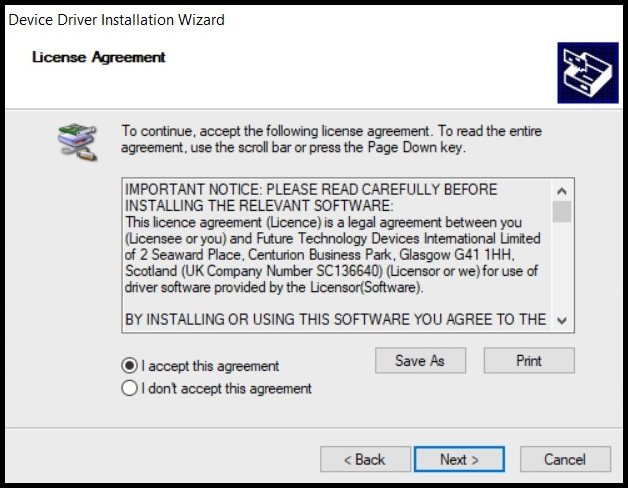
\includegraphics[width=0.6\linewidth]{images/img001_install_drivers_04.jpg}
  \end{center}
\end{minipage}

De installatie van de drivers wordt gestart.

\begin{minipage}{\linewidth}
  Klik op ``Finish''.
  \\
  \begin{center}
    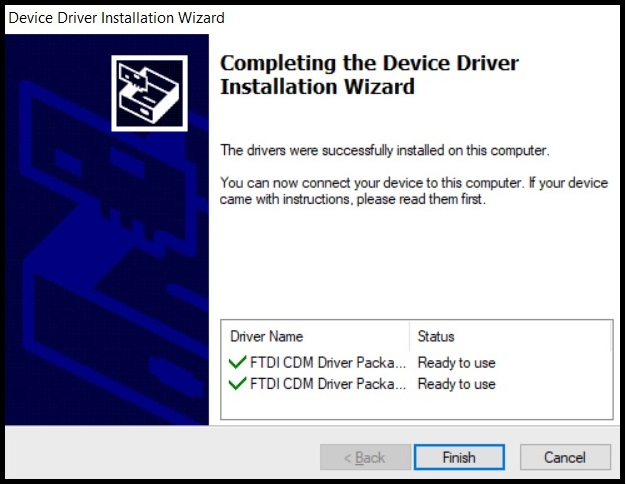
\includegraphics[width=0.6\linewidth]{images/img001_install_drivers_05.jpg}
  \end{center}
\end{minipage}

Sluit de USB-kabel aan op een USB-poort op de PC \textcolor{red}{zonder de Nexys4-plaat in te schakelen}.

Het aansluiten van de USB-kabel veroorzaakt het verschijnen van nieuwe apparaten.

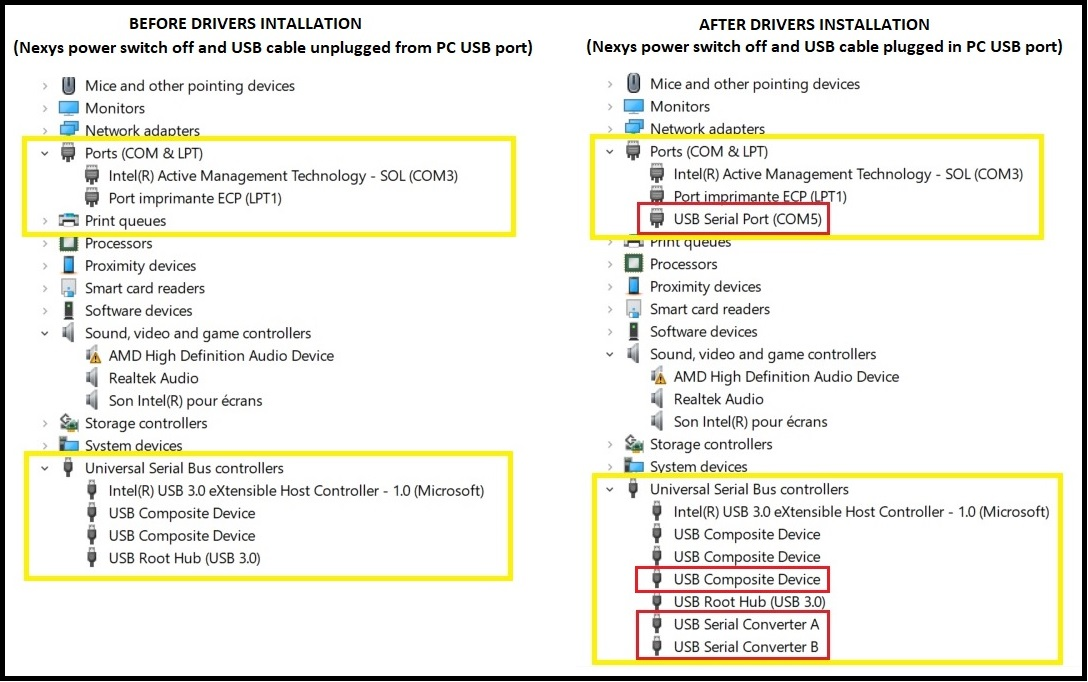
\includegraphics[width=\linewidth]{images/img001_install_drivers_07.jpg}

\begin{itemize}
  \item Er is een extra COM-poort geïnstalleerd: \textcolor{red}{dit is de COM-poort die gebruikt wordt om met de Nexys4-plaat te communiceren.}  \item Er is een extra USB-samengesteld apparaat geïnstalleerd.  \item Er zijn twee USB-serieel-omzetters geïnstalleerd.
\end{itemize}

Op dit moment is de Nexys4-plaat nog niet van stroom voorzien.

Voor meer informatie over de geïnstalleerde drivers kunt u de bijbehorende documentatie downloaden:

\begin{itemize}
  \item \url{https://ftdichip.com/wp-content/uploads/2020/08/AN\_396-FTDI-Drivers-Installation-Guide-for-Windows-10.pdf}
  \item \url{https://ftdichip.com/wp-content/uploads/2021/01/AN\_119\_FTDI\_Drivers\_Installation\_Guide\_for\_Windows7.pdf}
\end{itemize}

\section{De hoofd-FPGA flashen met Vivado}
\label{sec:mainfpgaflashing}

Ter verduidelijking: wanneer wij spreken over het ``flashen van de FPGA'', bedoelen wij in feite het flashen van het QSPI-flashgeheugen waarvan de FPGA bij het opstarten gebruikmaakt om de bitstream snel te laden.

De afbeelding hieronder toont twee veelgebruikte manieren waarop de FPGA bij het opstarten een bitstream kan laden:

\begin{center}
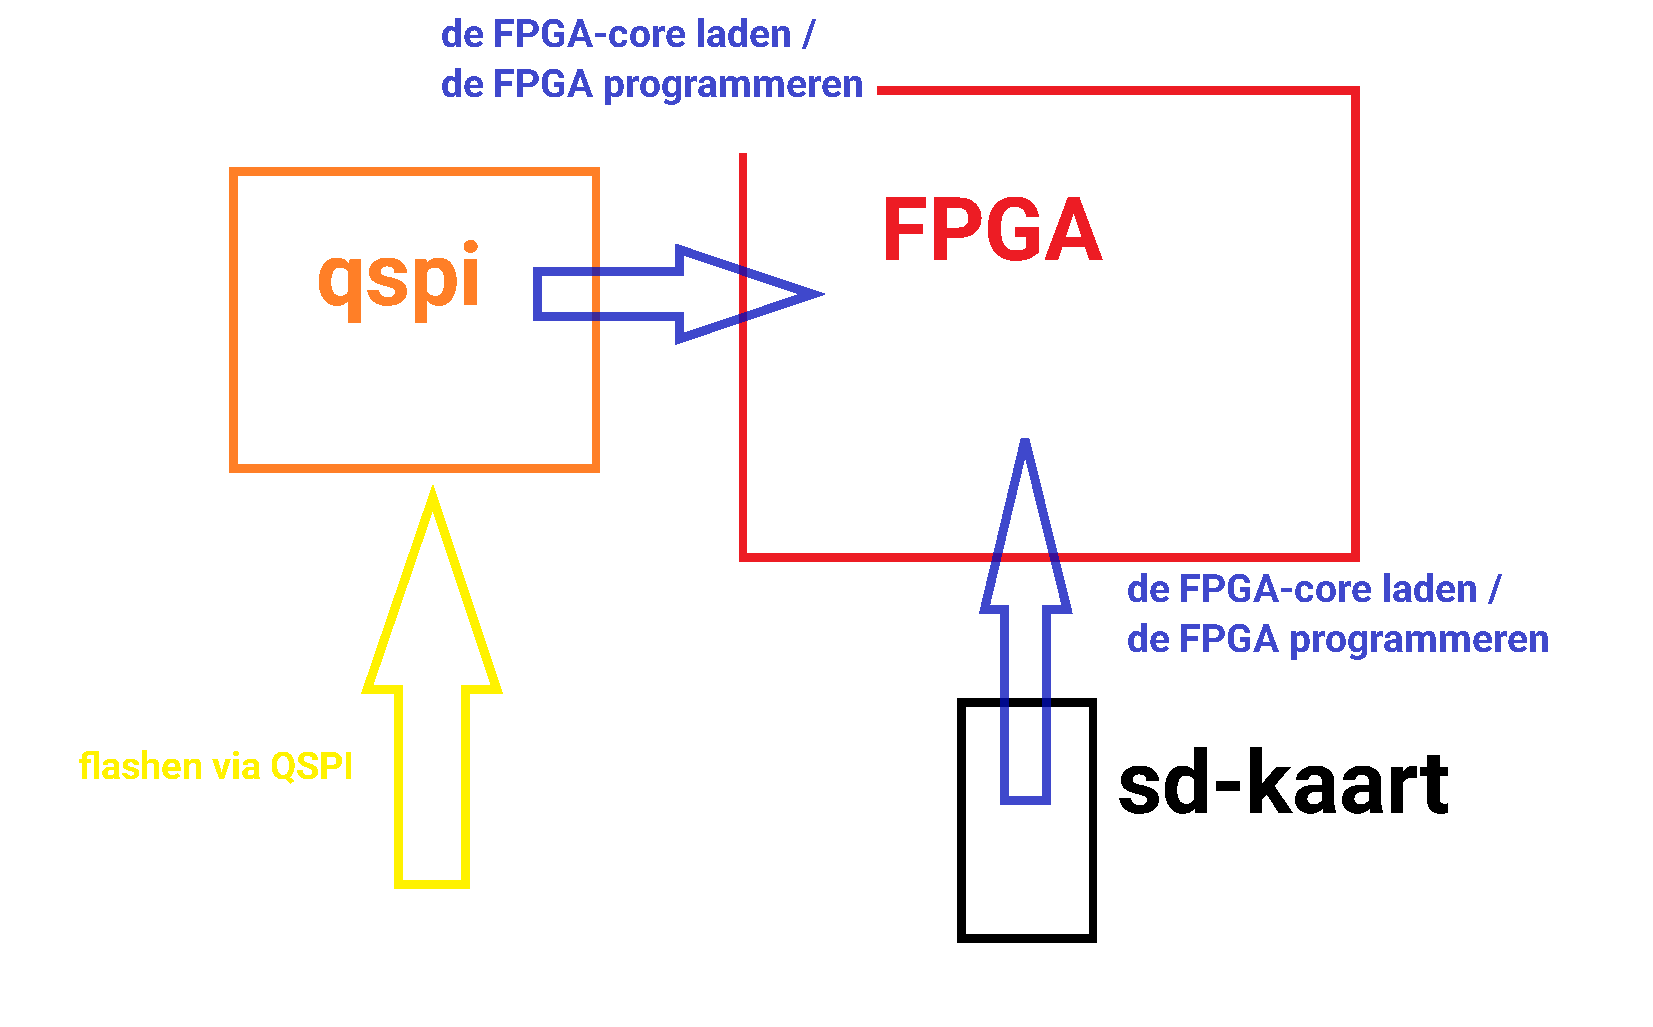
\includegraphics[width=0.8\linewidth]{dutch/images/flashing_fpga.pdf}
\end{center}

\begin{itemize}
  \item We kunnen eerst een bitstream-/core-bestand op het QSPI-flashgeheugen flashen, waarna de FPGA dit bij het opstarten snel kan laden. Het flashen van het QSPI is tamelijk traag, maar het voordeel van een korte opstarttijd is een duidelijke meerwaarde.  \item Gebruikers van een Nexys-plaat kunnen een bitstream-bestand op hun SD-kaart plaatsen en de FPGA dit (enigszins langzamer) bij het opstarten vanaf daar laten laden. Hierdoor kunnen bitstreams snel gewisseld of bijgewerkt worden zonder een TE0790-03 JTAG-programmeermodule. Deze functionaliteit is echter voor later gepland voor de MEGA65.
\end{itemize}

In dit onderdeel beschrijven wij de werkwijze die gebruikmaakt van de QSPI.

Veel van de volgende stappen in dit onderdeel zijn van toepassing op eigenaren van zowel de MEGA65 R2/R3/R3A/R4 als op eigenaren van een Nexys4-plaat. Er zijn onderweg enkele verschillen waarvan de lezer op de hoogte gesteld zal worden.

Indien u ervoor kiest om verder te gaan, heeft u een functionele installatie van het Vivado-programma van Xilinx nodig en de FTDI-drivers zoals beschreven in de voorgaande onderdelen.

U moet ook een .mcs-bitstreambestand downloaden of zelf bouwen (en een optioneel .prm-controlesomverificatiebestand) dat u via Vivado op de QSPI-chip wilt flashen. Zie het {\bf grote Mega65-boek} voor meer details over waar dergelijke bestanden gedownload kunnen worden.

\begin{tcolorbox}[colback=white,coltext=black]
\underline{Voor eigenaren van de MEGA65 R2/R3/R3A/R4}:\\
\\
U heeft een TE0790-03 JTAG-programmeermodule nodig. Het is ook noodzakelijk dat dip-schakelaars 1 en 3 op de AAN-stand staan en dip-schakelaars 2 en 4 op de UIT-stand op de TE-0790. Met de MEGA65 losgekoppeld van de voeding moet de TE-0790 op de JB1-connector worden geïnstalleerd, die zich tussen de diskettedatakabel en de audiojack bevindt. De vergulde opening van de TE-0790 moet in lijn liggen met het schroefgat eronder. De mini-USB-kabel verbindt zich vervolgens aan de kant richting het 3.5'' diskettestation. De volgende afbeelding toont de juiste positie: de TE0790 is omringd door de gele kast en de dip-schakelaars door de rode kast. Dip-schakelaar 1 is de dichtstbijzijnde bij de diskettedatakabel. \\
\\
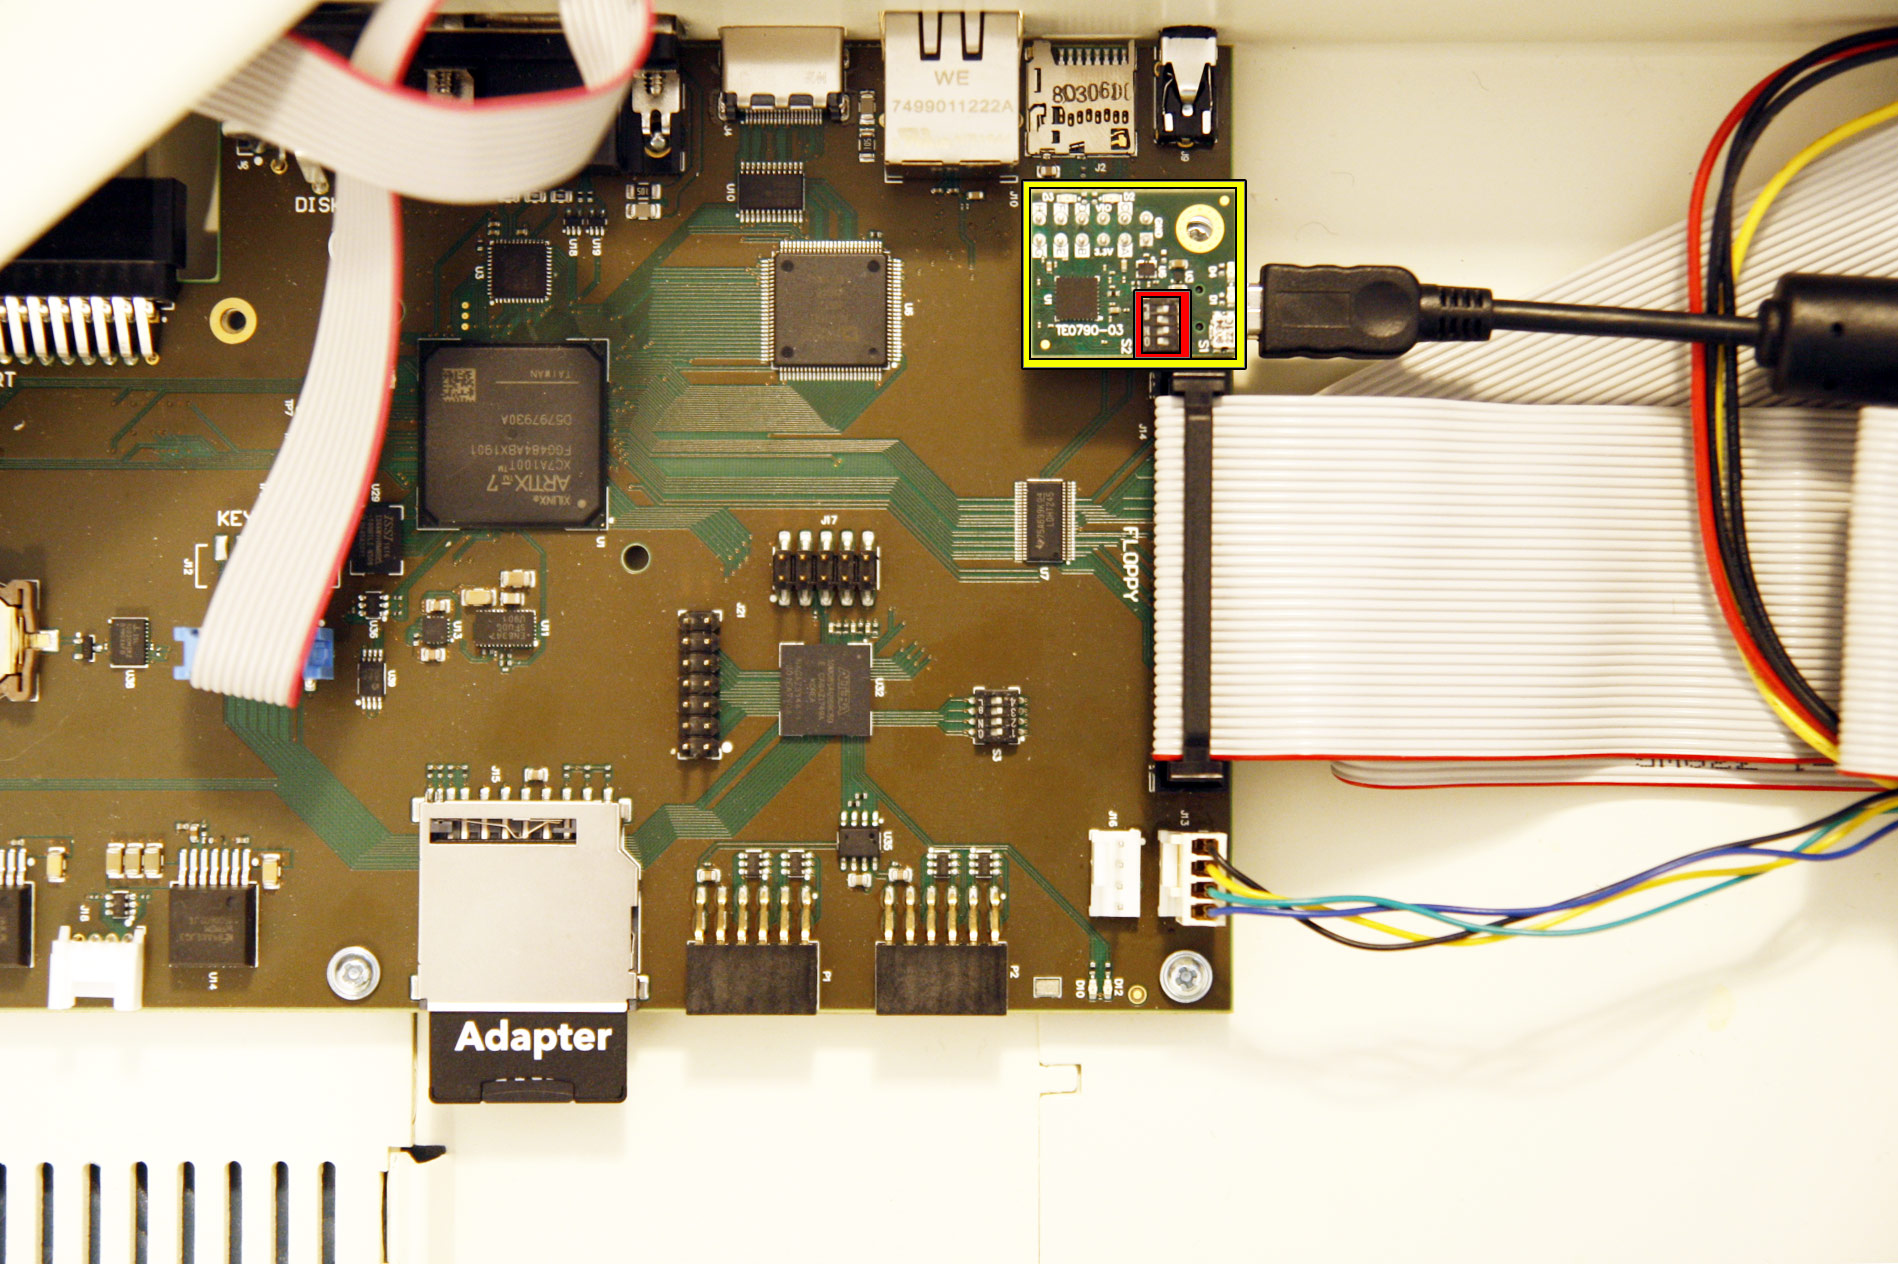
\includegraphics[width=\linewidth]{images/jtag_detail_02.jpg}
\end{tcolorbox}

\begin{tcolorbox}[colback=white,coltext=black]
\underline{Voor eigenaren van een Nexys4-bord}: \\
\\
  Sluit uw micro-USB-kabel aan tussen uw Nexys4-bord en uw pc via de poort met het label ``PROG UART'' (J6), zoals getoond: \\
\\
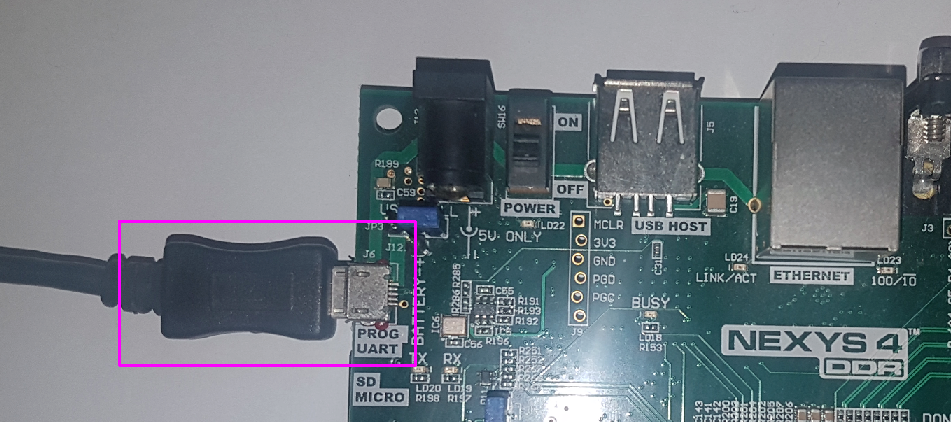
\includegraphics[width=\linewidth]{images/nexys4_comms.png}
\\
\\
Zet bovendien de J1-jumper op de QSPI-stand:
\\
\begin{center}
  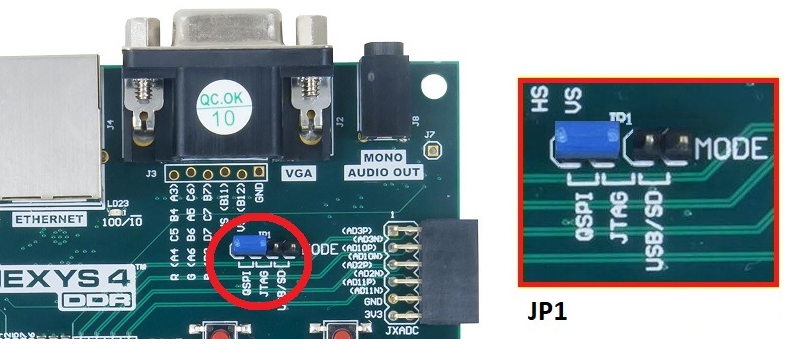
\includegraphics[width=0.8\linewidth]{images/nexys4_j2.png}
\end{center}

\end{tcolorbox}

\begin{itemize}
  \item Sluit uw niet-8-bit computer aan op het FPGA-programmeerapparaat met behulp van de juiste USB-kabel.  \item Schakel de MEGA65-computer in.  \item Open Vivado.
\end{itemize}


\begin{minipage}{\linewidth}
  Stap 1a: Maak een nieuw Vivado-project aan via ``File'', ``Project'', ``New...''. \\  LET OP: Bij toekomstige gelegenheden waarop u de QSPI moet flashen, heropent u dit project (het is niet nodig elke keer een nieuw project aan te maken).  \\
  \begin{center}
    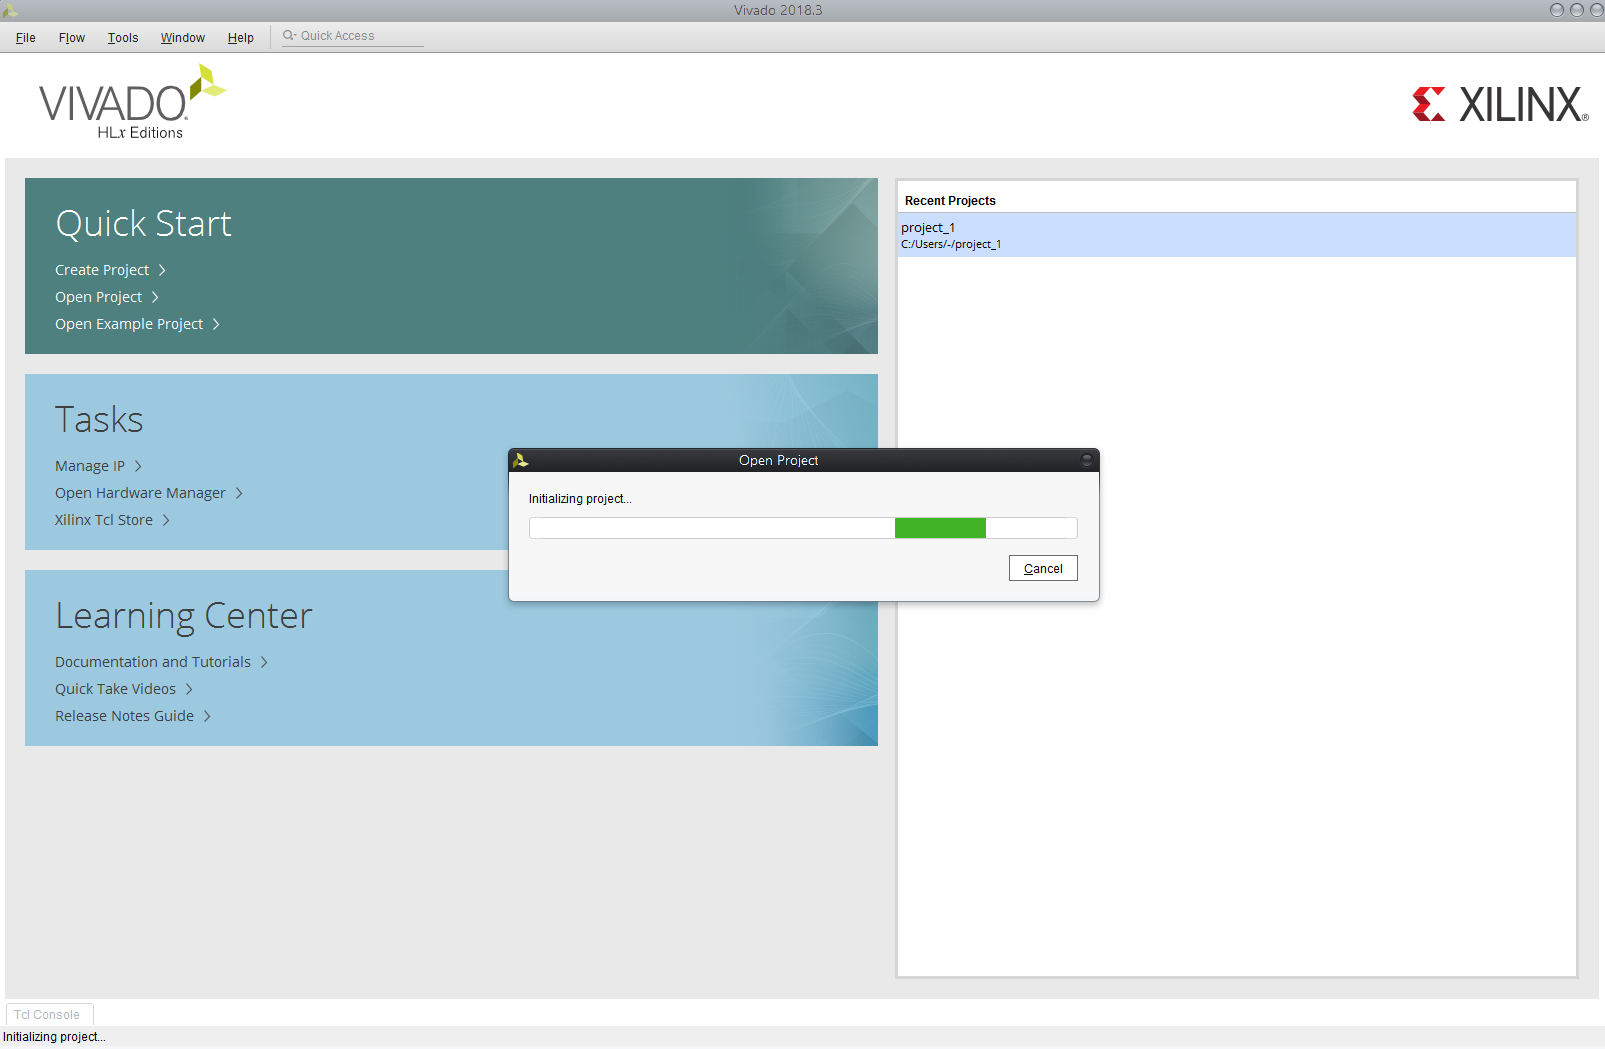
\includegraphics[width=0.8\linewidth]{images/vivado01.png}
  \end{center}
\end{minipage}

\vspace{5mm}

\begin{minipage}{\linewidth}
  Stap 1b: De wizard ``New Project'' verschijnt. Klik op ``Next'': \\
  \begin{center}
    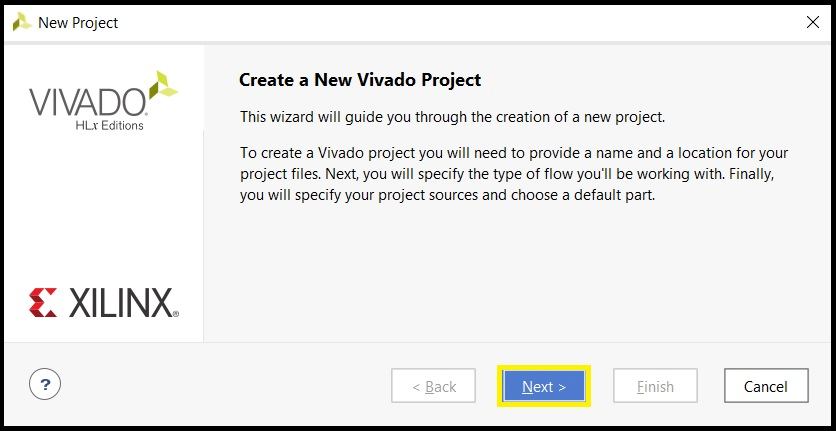
\includegraphics[width=0.8\linewidth]{images/vivado01b.png}
  \end{center}
\end{minipage}

\begin{minipage}{\linewidth}
  Stap 1c: Geef uw project een naam en kies de gewenste locatie en klik op ``Next'':\\
  \begin{center}
    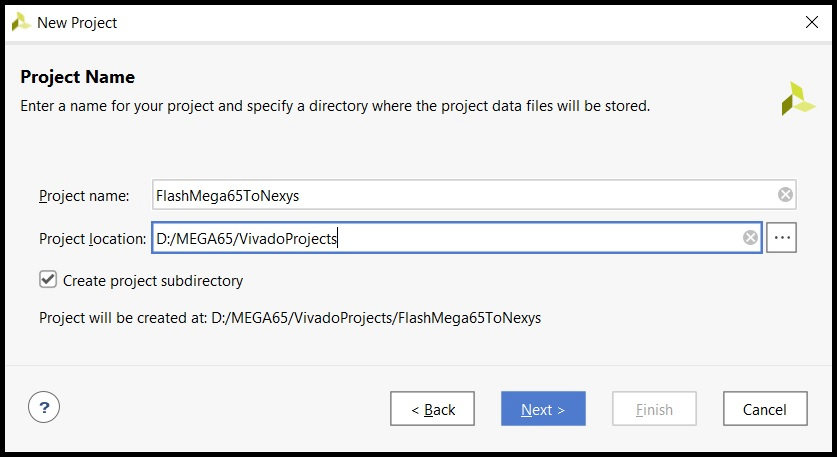
\includegraphics[width=0.8\linewidth]{images/vivado01c.png}
  \end{center}
\end{minipage}

\vspace{5mm}

\begin{minipage}{\linewidth}
  Stap 1d: Laat de standaard geselecteerde opties behouden en klik op ``Next'': \\
  \begin{center}
    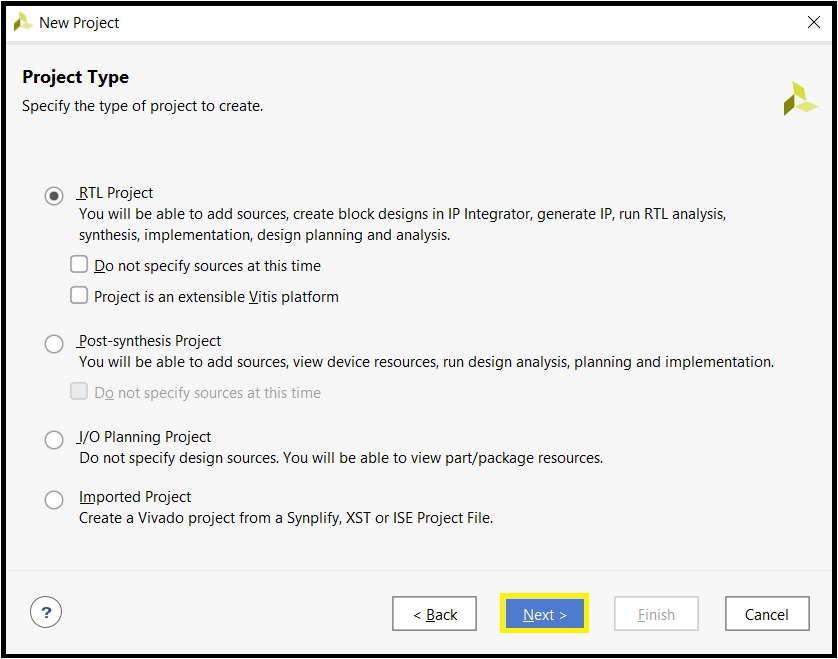
\includegraphics[width=0.8\linewidth]{images/vivado01d.png}
  \end{center}
\end{minipage}

\begin{minipage}{\linewidth}
  Stap 1e: Voeg geen bronnen toe, laat de standaard geselecteerde opties behouden en klik op ``Next'': \\
  \begin{center}
    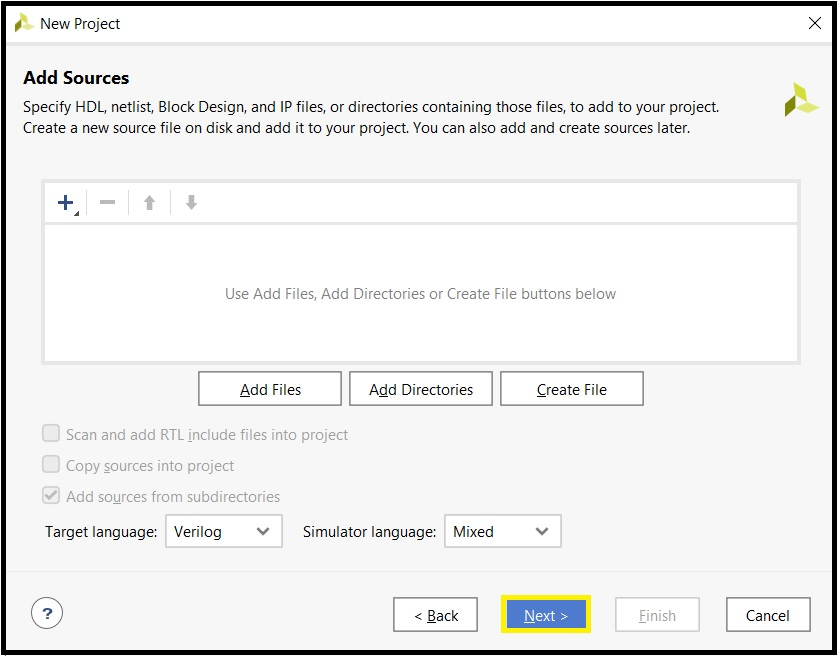
\includegraphics[width=0.7\linewidth]{images/vivado01e.png}
  \end{center}
\end{minipage}

\vspace{5mm}

\begin{minipage}{\linewidth}
  Stap 1f: Laat de standaard geselecteerde opties behouden en klik op ``Next'': \\
  \begin{center}
    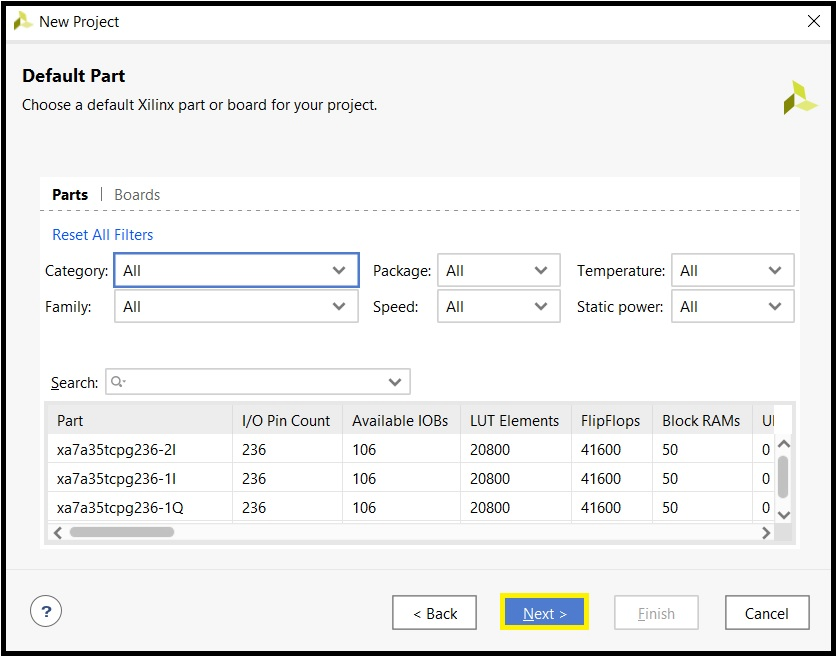
\includegraphics[width=0.7\linewidth]{images/vivado01f.png}
  \end{center}
\end{minipage}

\begin{minipage}{\linewidth}
  Stap 1g: Klik op ``Finish'': \\
  \begin{center}
    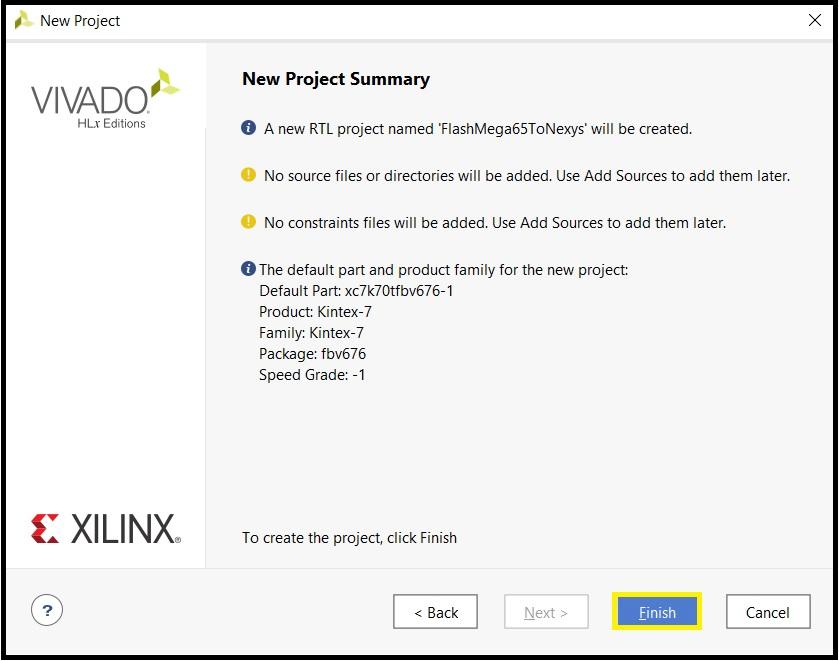
\includegraphics[width=0.8\linewidth]{images/vivado01g.png}
  \end{center}
\end{minipage}

\vspace{5mm}

\begin{minipage}{\linewidth}
  Stap 2: Selecteer in de linker kolom ``Open Hardware Manager'' helemaal onderaan.
  \\
  \begin{center}
    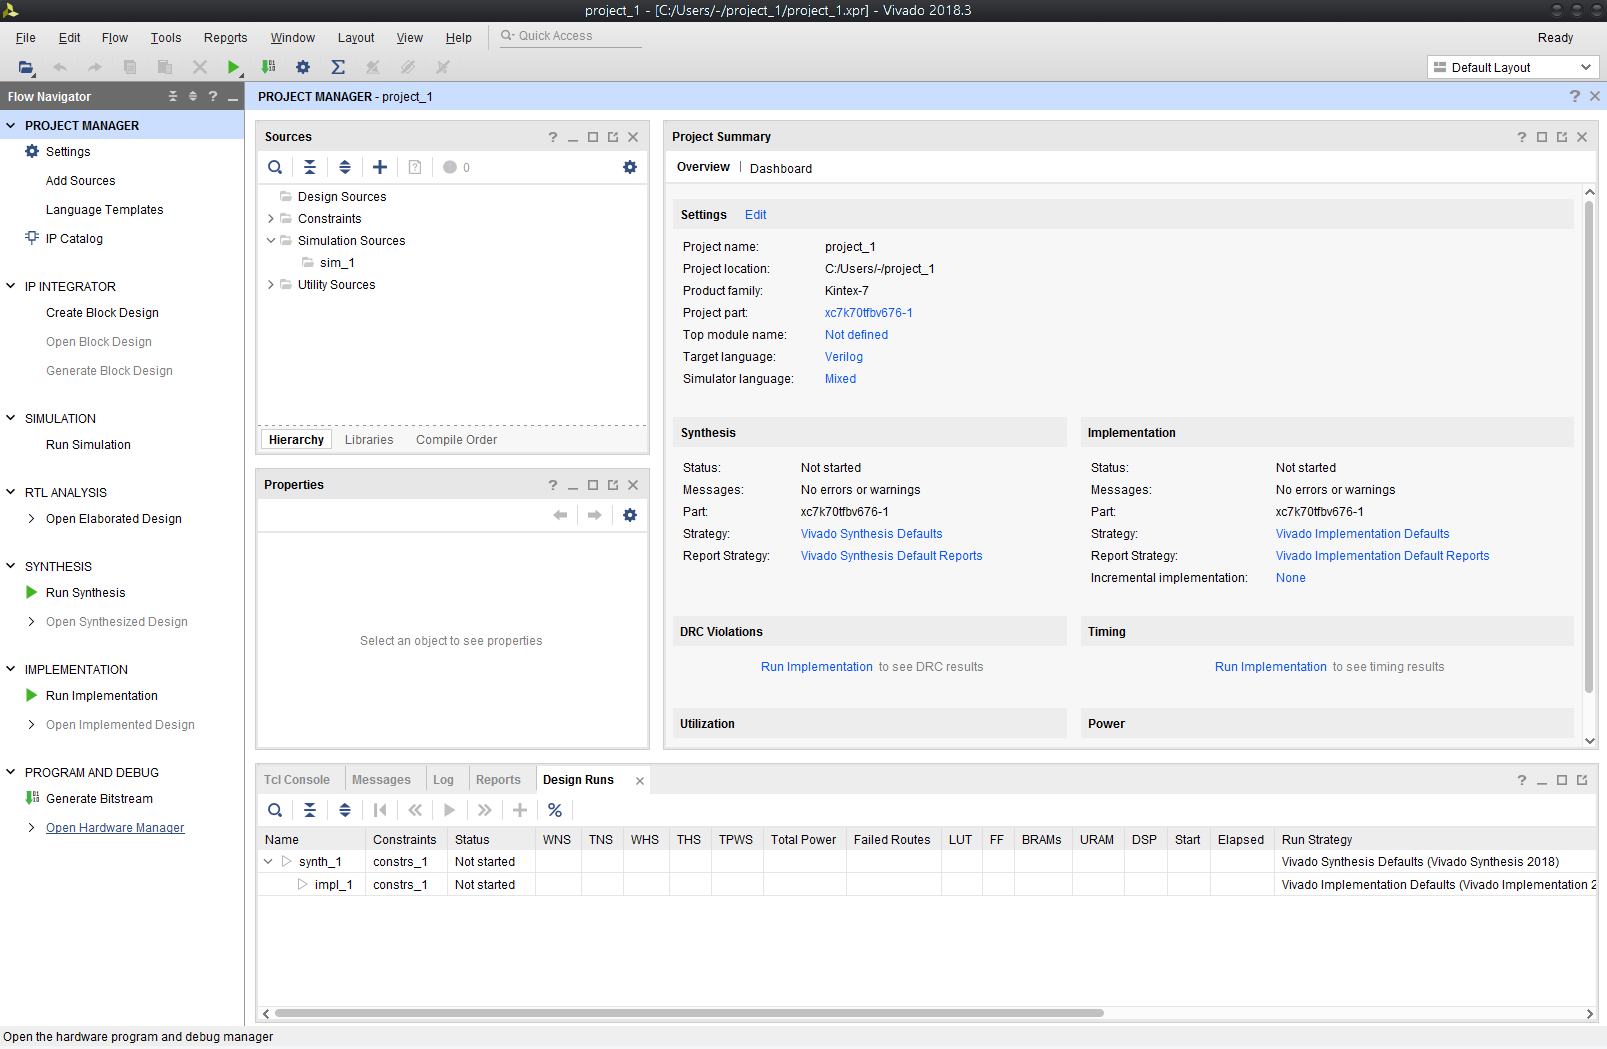
\includegraphics[width=0.8\linewidth]{images/vivado02.png}
  \end{center}
\end{minipage}


\begin{minipage}{\linewidth}
  Stap 3: Verbind met de FPGA: \\  Onder ``Open Hardware Manager'' kiest u ``Open Target'' en vervolgens ``Auto Connect''.
  \\
  \begin{center}
    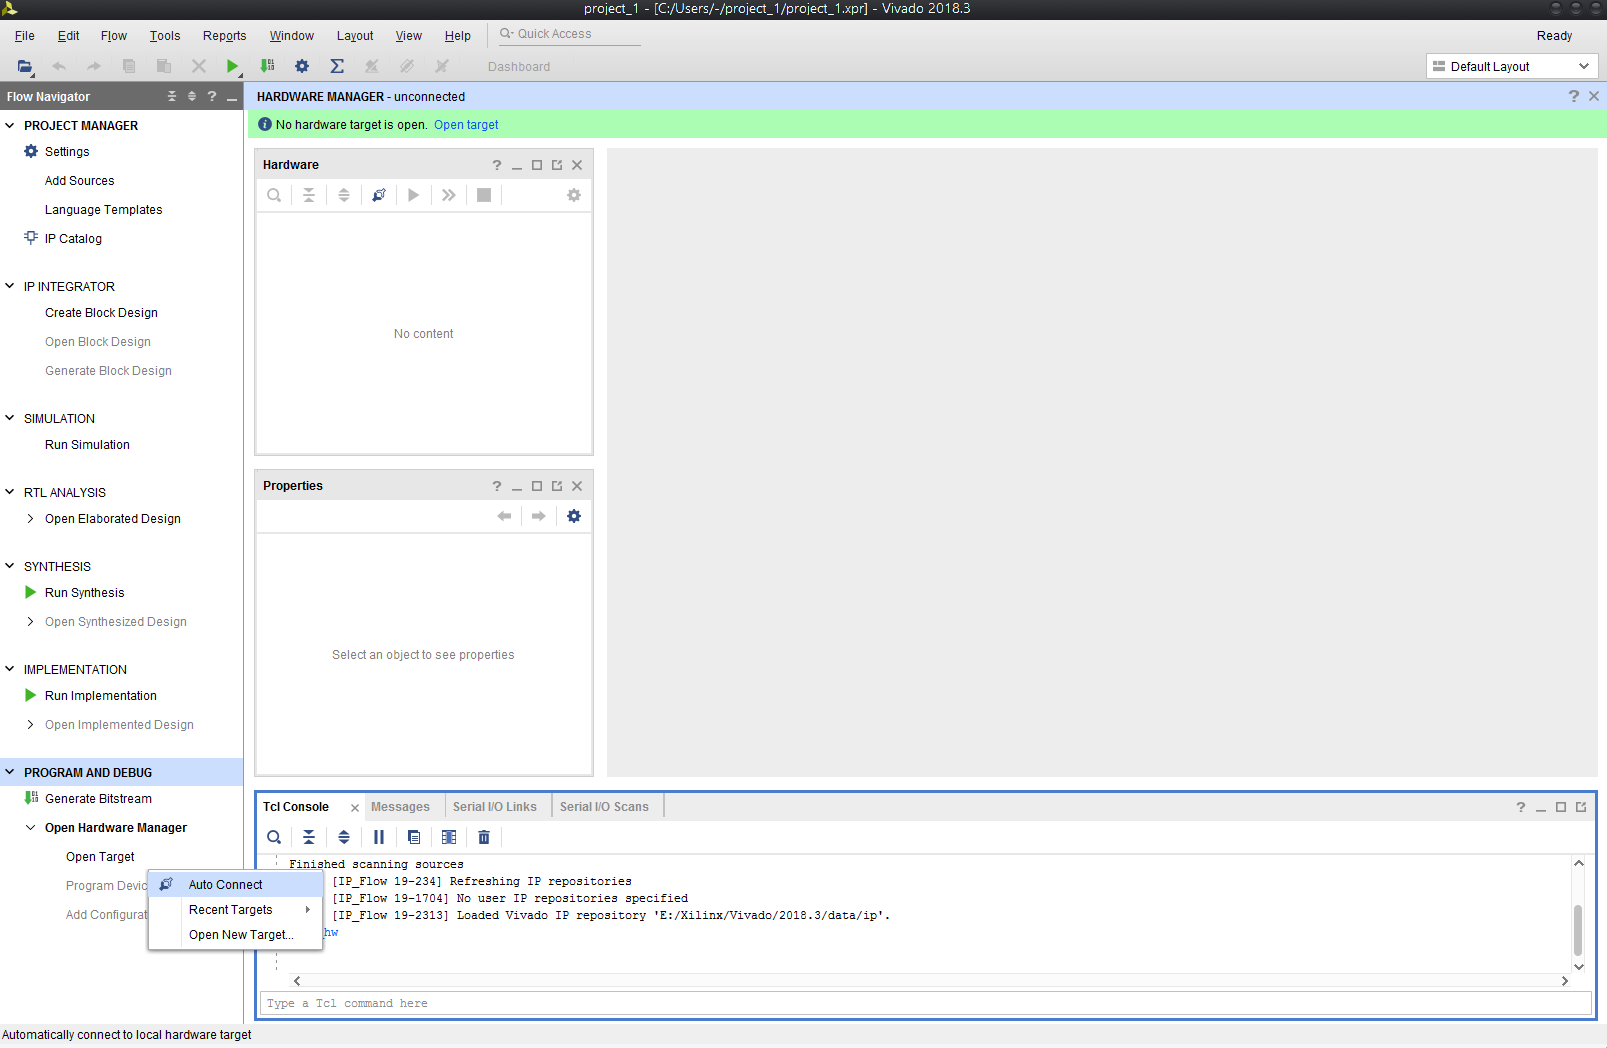
\includegraphics[width=0.8\linewidth]{images/vivado03.png}
  \end{center}
\end{minipage}

\vspace{5mm}

\begin{minipage}{\linewidth}
  Stap 4: Wacht even; ``Connecting to server...'' zou automatisch moeten sluiten zonder een foutmelding aan de console te geven.
  \\
  \begin{center}
    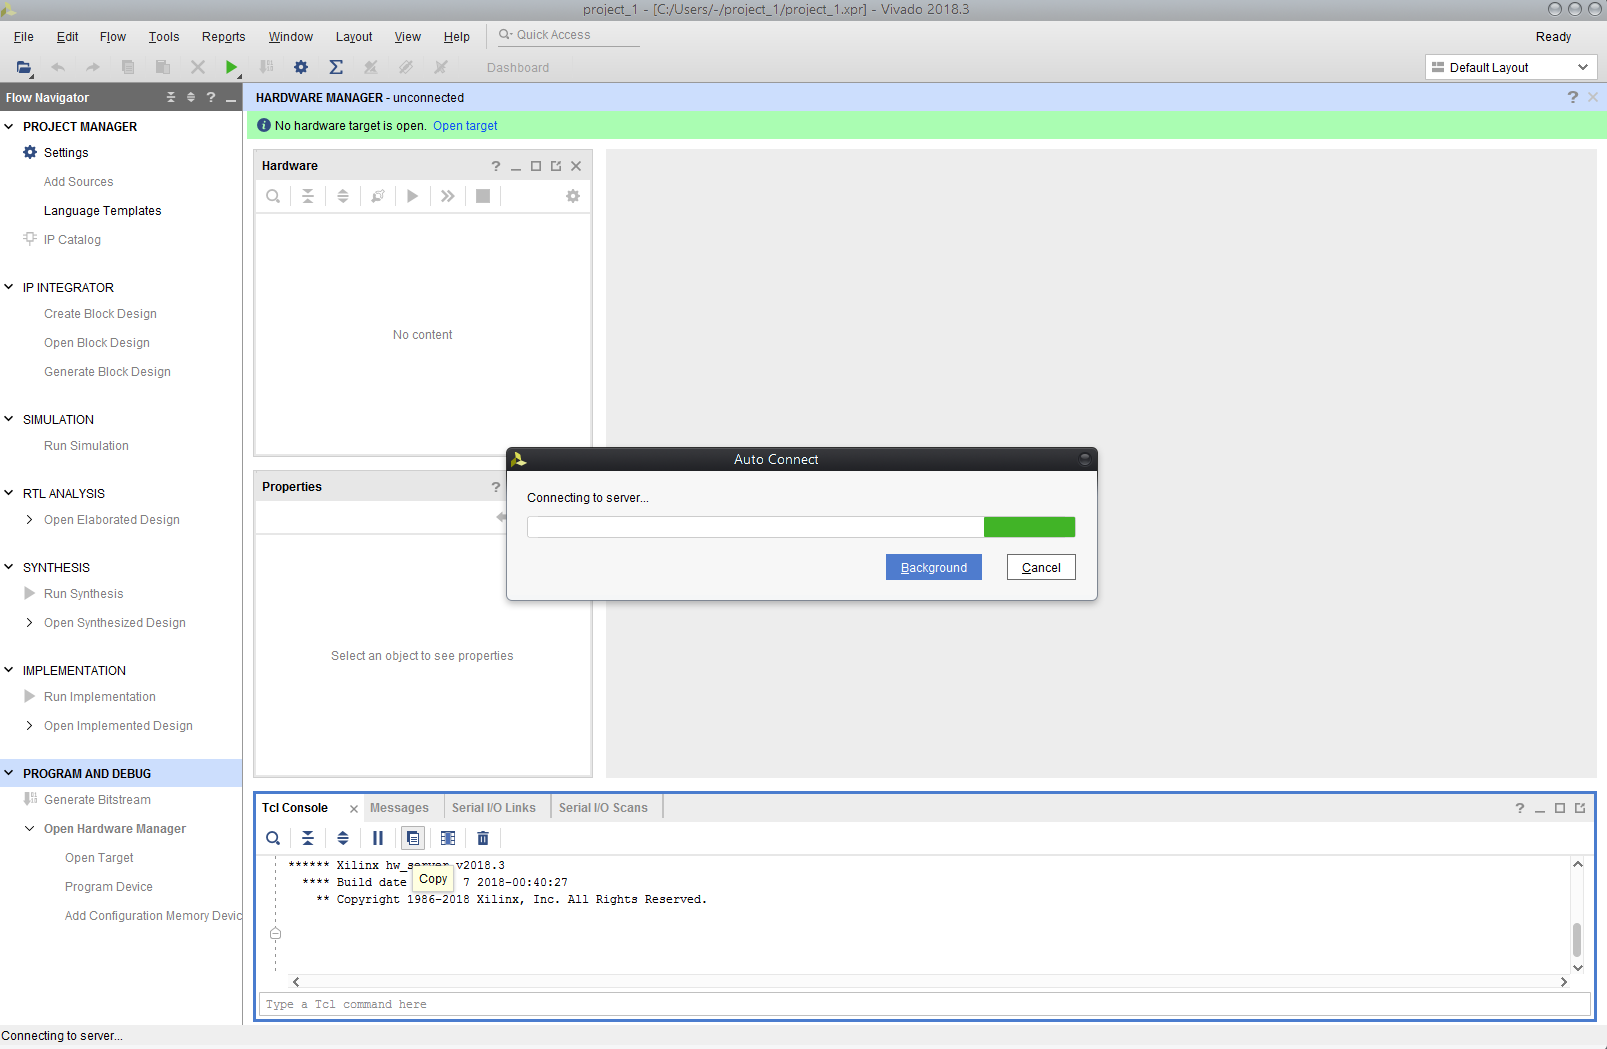
\includegraphics[width=0.8\linewidth]{images/vivado04.png}
  \end{center}
\end{minipage}


\begin{minipage}{\linewidth}
  Stap 5: Onder ``Open Hardware Manager'' kiest u ``Add Configuration Memory Device'' en vervolgens:
  \begin{itemize}
    \item \underline{Voor MEGA65R3/R3A/R4}: ``xc7a200t\_0''    \item \underline{Voor Nexys4 en MEGA65R2}: ``xc7a100t\_0''.
  \end{itemize}

  \begin{center}
    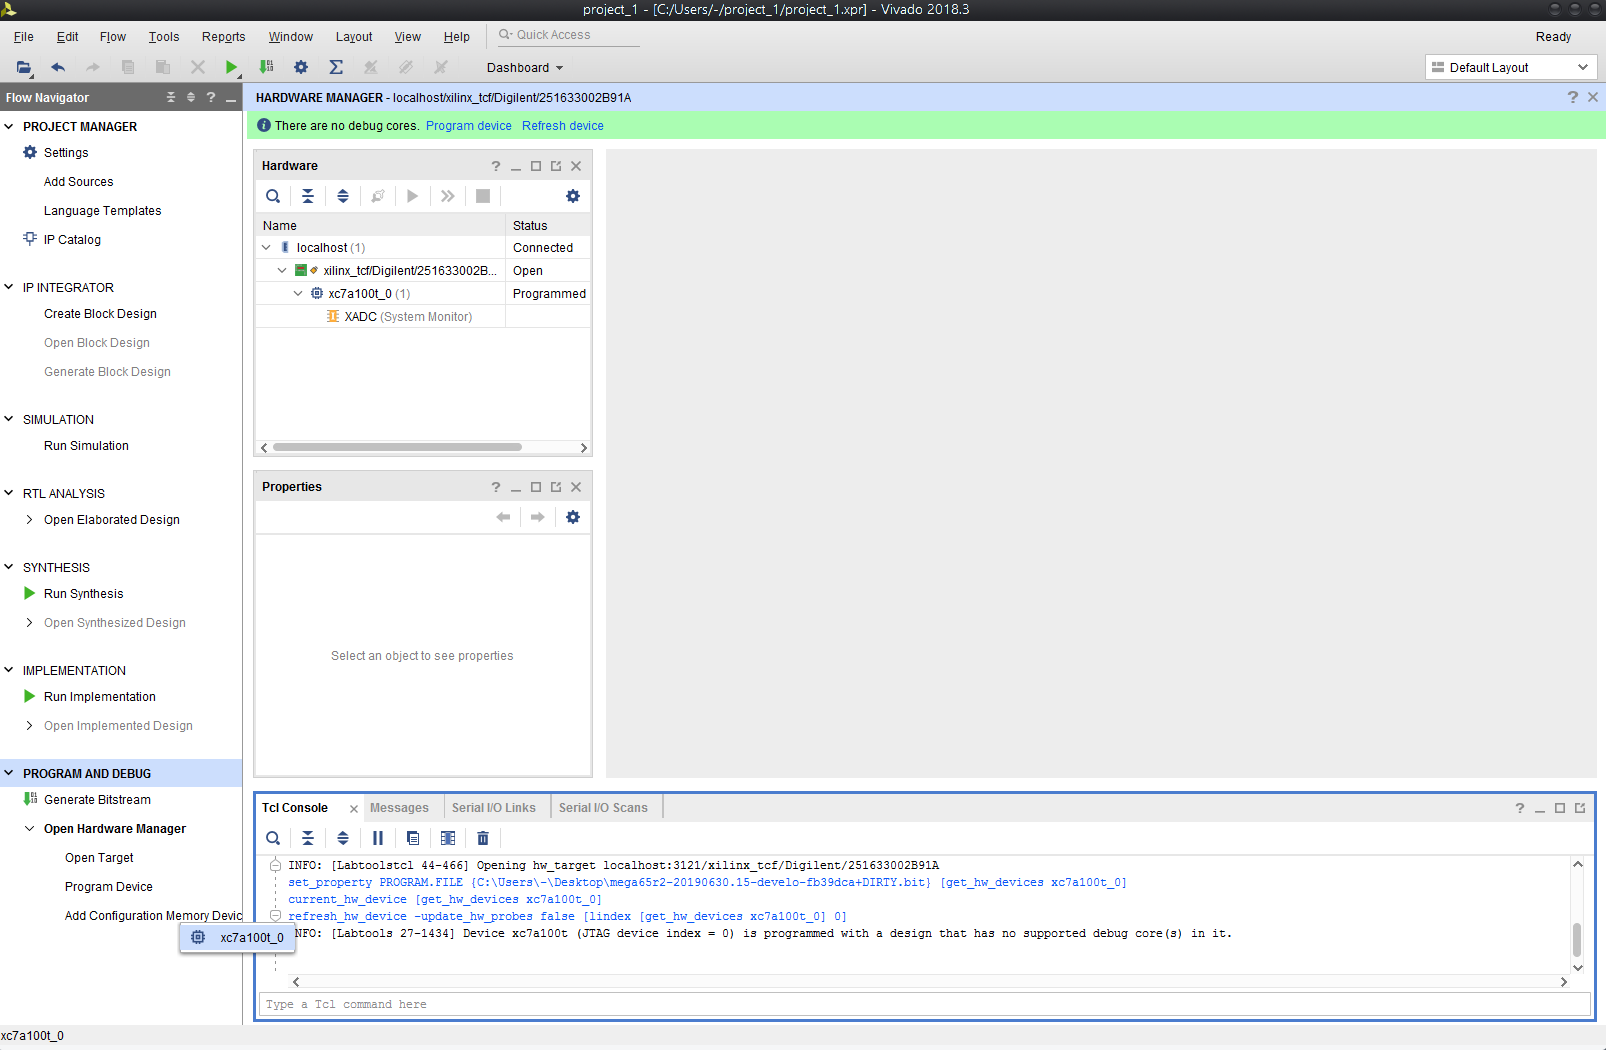
\includegraphics[width=0.7\linewidth]{images/vivado05.png}
  \end{center}
\end{minipage}

\vspace{5mm}

\begin{minipage}{\linewidth}
  Stap 6a: Selecteer Memory Part: \\
  \\
  In het nieuw geopende dialoogvenster:
  \begin{itemize}
    \item \underline{Voor MEGA65R2/R3}: typ ``S25fl256s''    (zonder aanhalingstekens), selecteer vervolgens ``s25fl256sxxxxxxx0-spi-x1\_x2\_x4''    (de bovenste) en klik op ``OK''.    \item \underline{Voor MEGA65R3A/R4}: Vivado kan het grotere flashgeheugen op deze borden niet flashen. Gebruik het flashmenu op de MEGA65.    \item \underline{Voor Nexys4}: typ ``S25fl128s''    (zonder aanhalingstekens), selecteer vervolgens ``s25fl128sxxxxxxx0-spi-x1\_x2\_x4''    (de bovenste) en klik op ``OK''.
  \end{itemize}

  \begin{center}
    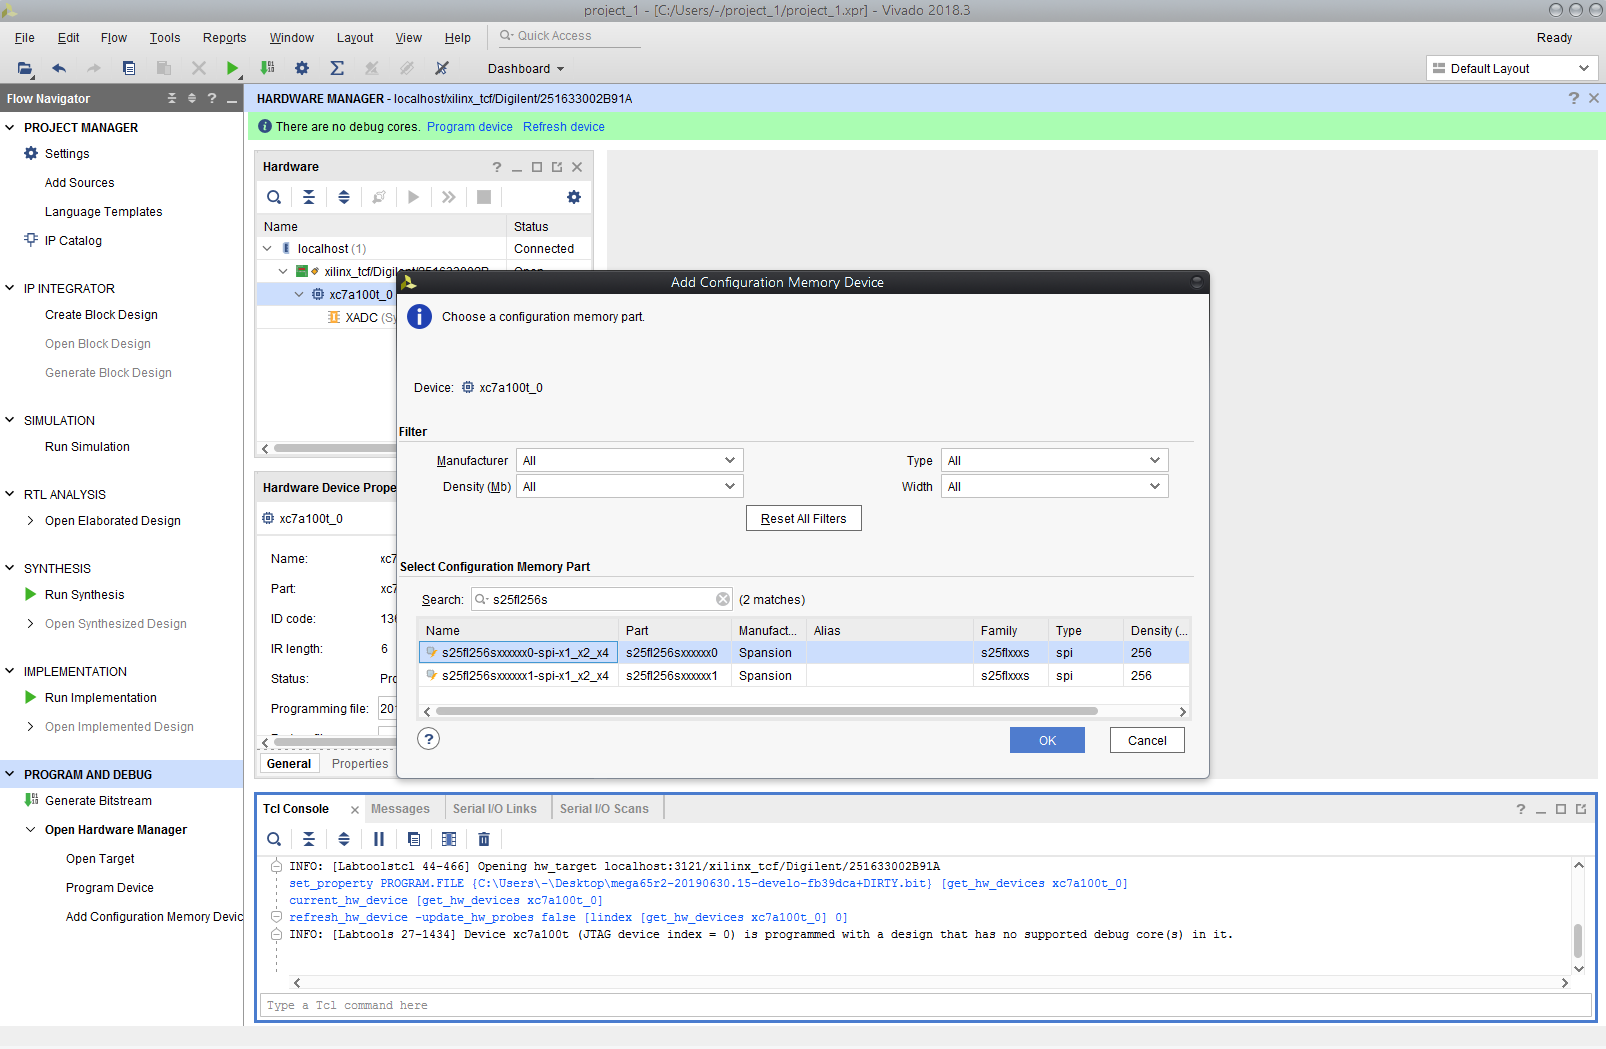
\includegraphics[width=0.7\linewidth]{images/vivado06.png}
  \end{center}
\end{minipage}

\begin{minipage}{\linewidth}
  Stap 6b: Klik op ``OK'' om te bevestigen dat u het configuratiegeheugenapparaat nu wilt programmeren.
  \begin{center}
    \includegraphics[width=0.85\linewidth]{images/vivado06b.png}
  \end{center}
\end{minipage}

\begin{minipage}{\linewidth}
  Stap 6c: Als u zo'n pop-up niet ziet of de QSPI op een later tijdstip opnieuw wilt programmeren, klikt u in het ``Hardware''-venster met de rechtermuisknop op de geheugenconfiguratie en selecteert u ``Program Configuration Memory Device'':
  \begin{center}
    \includegraphics[width=0.85\linewidth]{images/vivado06c.png}
  \end{center}
\end{minipage}

\begin{minipage}{\linewidth}
  Stap 7: Stel de programmeeropties in: \\  Stel in het volgende dialoogvenster ``Configuration file'' in op het pad van uw ``.mcs''-bitstream-bestand. U kunt optioneel ook het ``PRM file''-veld instellen op het pad van uw ``.prm''-bestand. Laat alle overige parameters zoals ze zijn (zie onderstaande screenshot).
  \\
  \begin{center}
    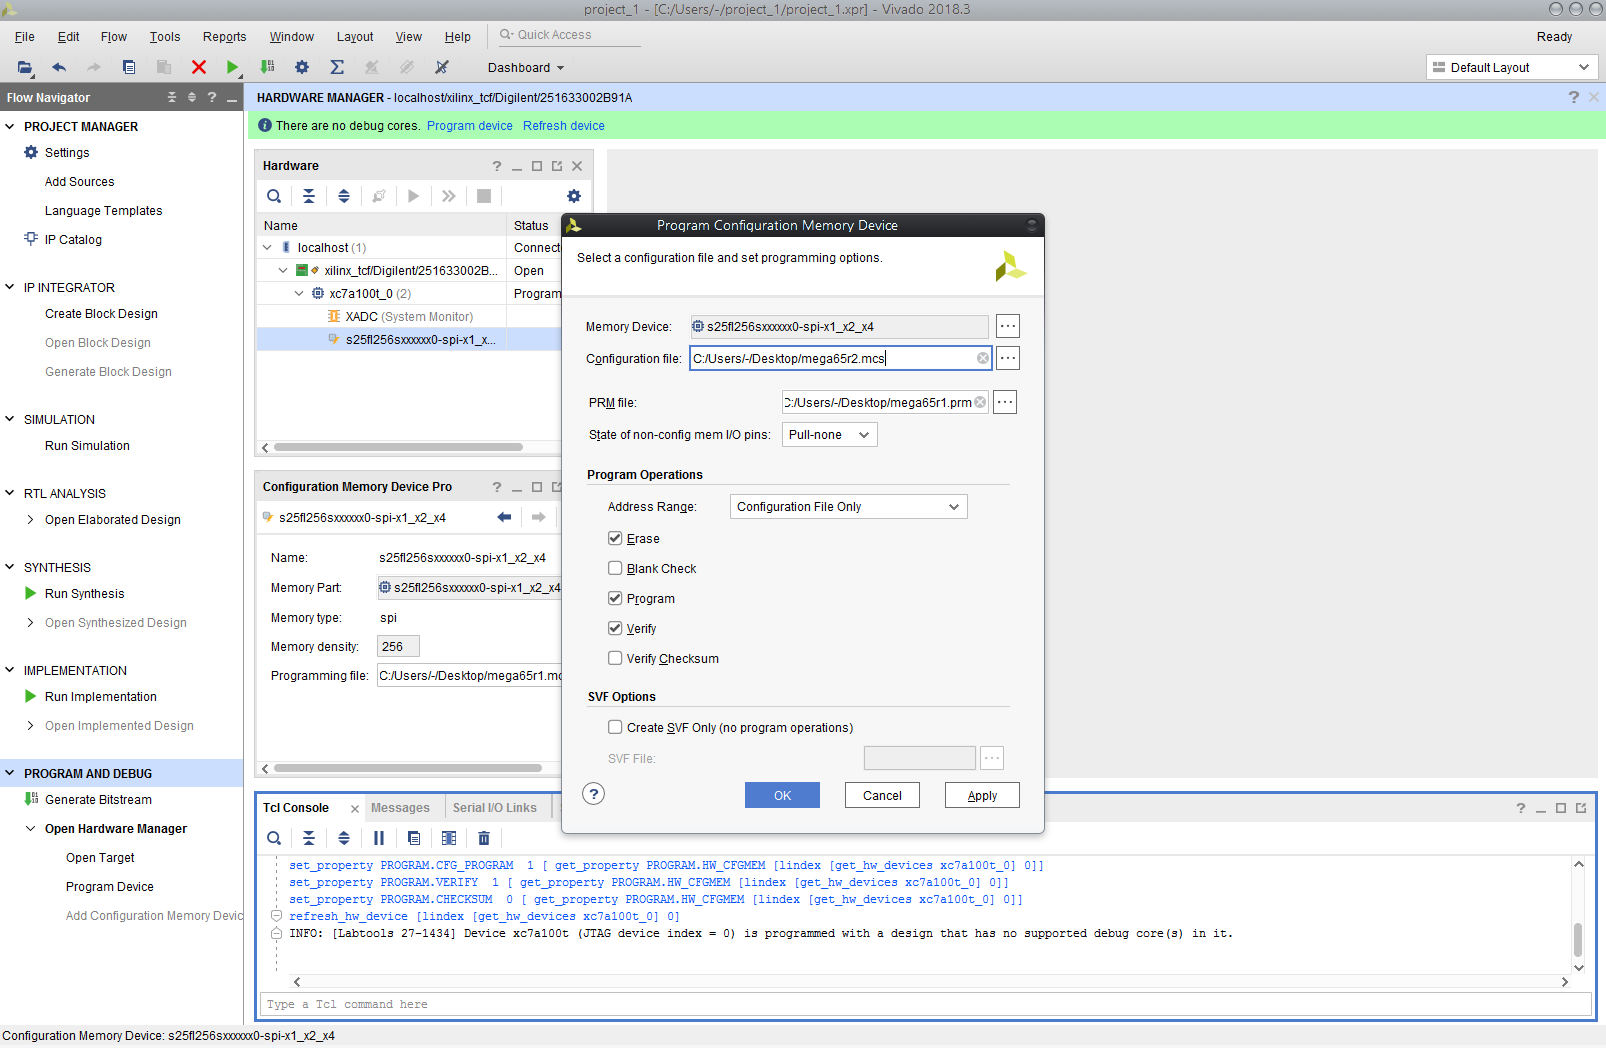
\includegraphics[width=0.85\linewidth]{images/vivado07.png}
  \end{center}
\end{minipage}

\vspace{1mm}

\begin{minipage}{\linewidth}
  Stap 8: Wacht geduldig tot het programmeren is voltooid.  Dit kan enkele minuten duren, omdat de Vivado-software het flashgeheugen dat wordt gebruikt om de FPGA bij het inschakelen te initialiseren, eerst wist en vervolgens opnieuw programmeert.
  \\
  \begin{center}
    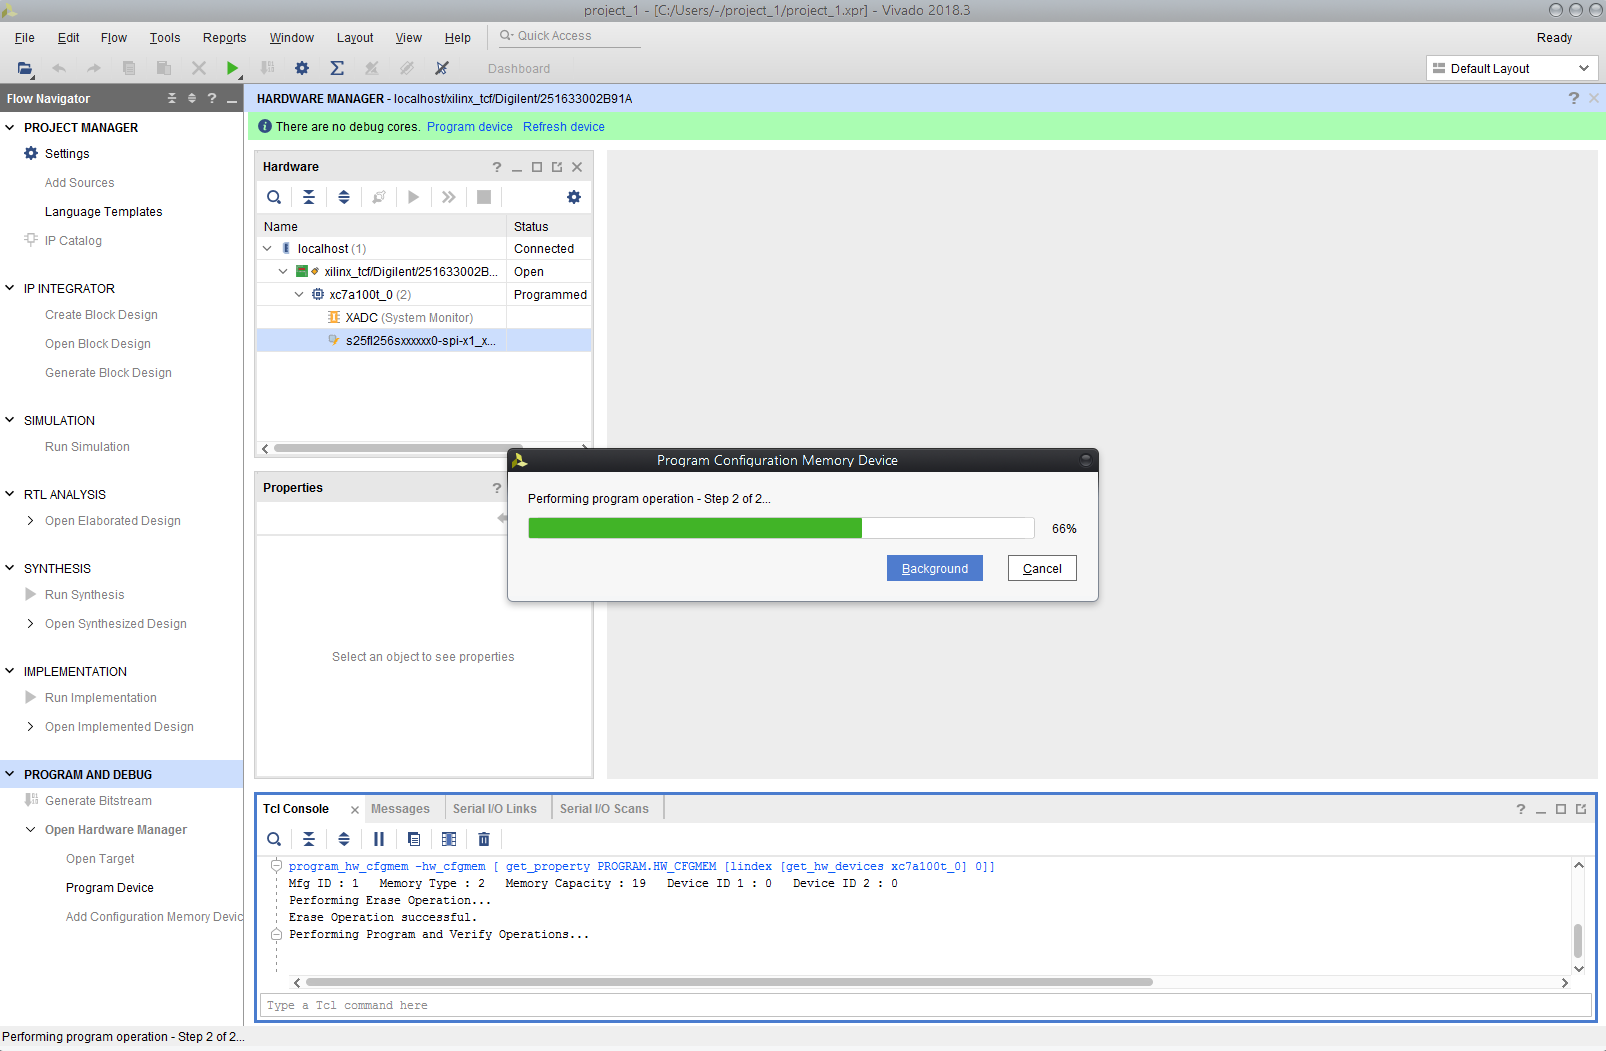
\includegraphics[width=0.85\linewidth]{images/vivado08.png}
  \end{center}
\end{minipage}


\begin{minipage}{\linewidth}
Stap 9: Als uw scherm eruitziet als de onderstaande screenshot, is uw nieuwe bitstream succesvol geflasht in Slot 0 van uw QSPI-flashgeheugen!
  \\
  \begin{center}
    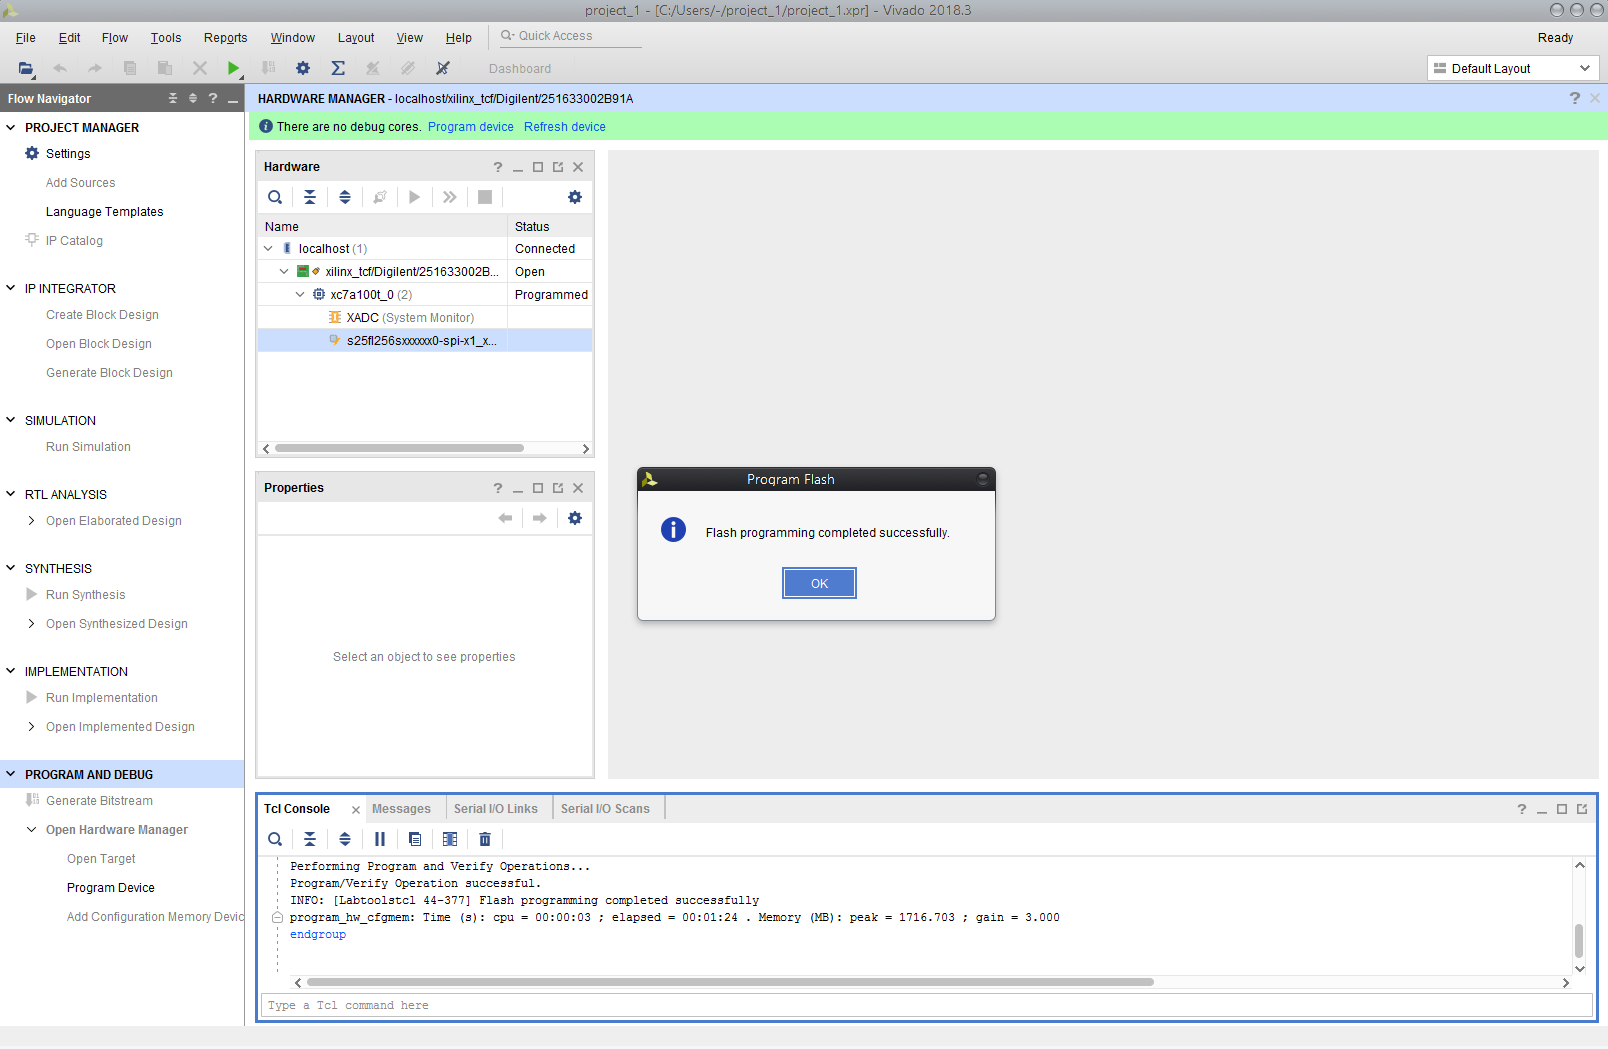
\includegraphics[width=0.8\linewidth]{images/vivado09.png}
  \end{center}
\end{minipage}

\vspace{5mm}

\begin{minipage}{\linewidth}
Stap 10: Als u de FPGA opnieuw wilt flashen, kan het zijn dat de optie ``Add Configuration Memory Device'' uit stap 5 grijs weergegeven wordt.
Selecteer in dat geval ``s25fl256sxxxxxxx0-spi-x1\_x2\_x4''  in het ``Hardware''-venster, druk op de rechtermuisknop en selecteer ``Program Configuration Memory Device'' om te flashen.
  \\
  \begin{center}
    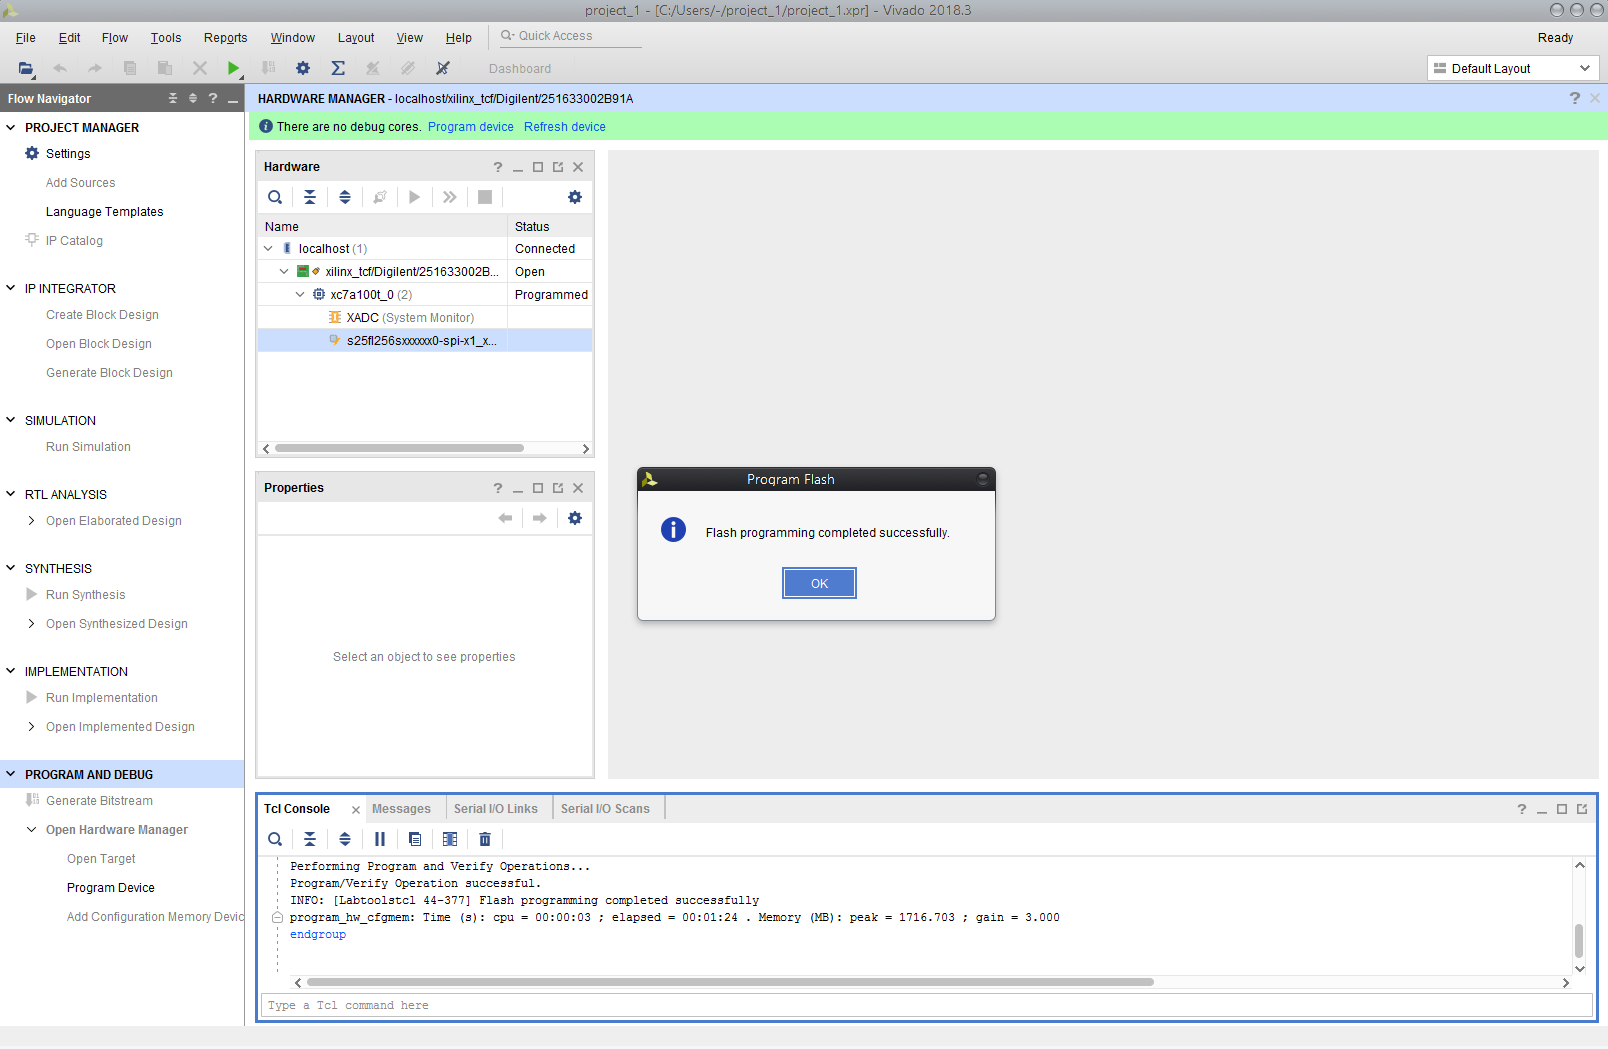
\includegraphics[width=0.8\linewidth]{images/vivado09.png}
  \end{center}
\end{minipage}


\section{De CPLD in het toetsenbord van de MEGA65 flashen met Lattice Diamond}
\label{sec:flashcpld}


Indien u ervoor kiest om door te gaan, heeft u een TE0790-03 JTAG-programmeermodule en een werkende installatie van Lattice Diamond Programmer-software nodig. Dit kan op zowel Windows als Linux, maar in beide gevallen moet u de benodigde USB-stuurprogramma's installeren. Het is ook noodzakelijk dat dip-schakelaars 1 en 3 op de AAN-stand staan en dip-schakelaars 2 en 4 op de UIT-stand op de TE-0790. Met de MEGA65 losgekoppeld van de voeding moet de TE-0790 op de JB1-connector worden geïnstalleerd, die zich tussen de diskettedatakabel en de audiojack bevindt. De vergulde opening van de TE-0790 moet in lijn liggen met het schroefgat eronder. De mini-USB-kabel verbindt zich vervolgens aan de kant richting het 3.5'' diskettestation. De volgende afbeelding toont de juiste positie: de TE0790 is omringd door de gele kast en de dip-schakelaars door de rode kast. Dip-schakelaar 1 is de dichtstbijzijnde bij de diskettedatakabel.


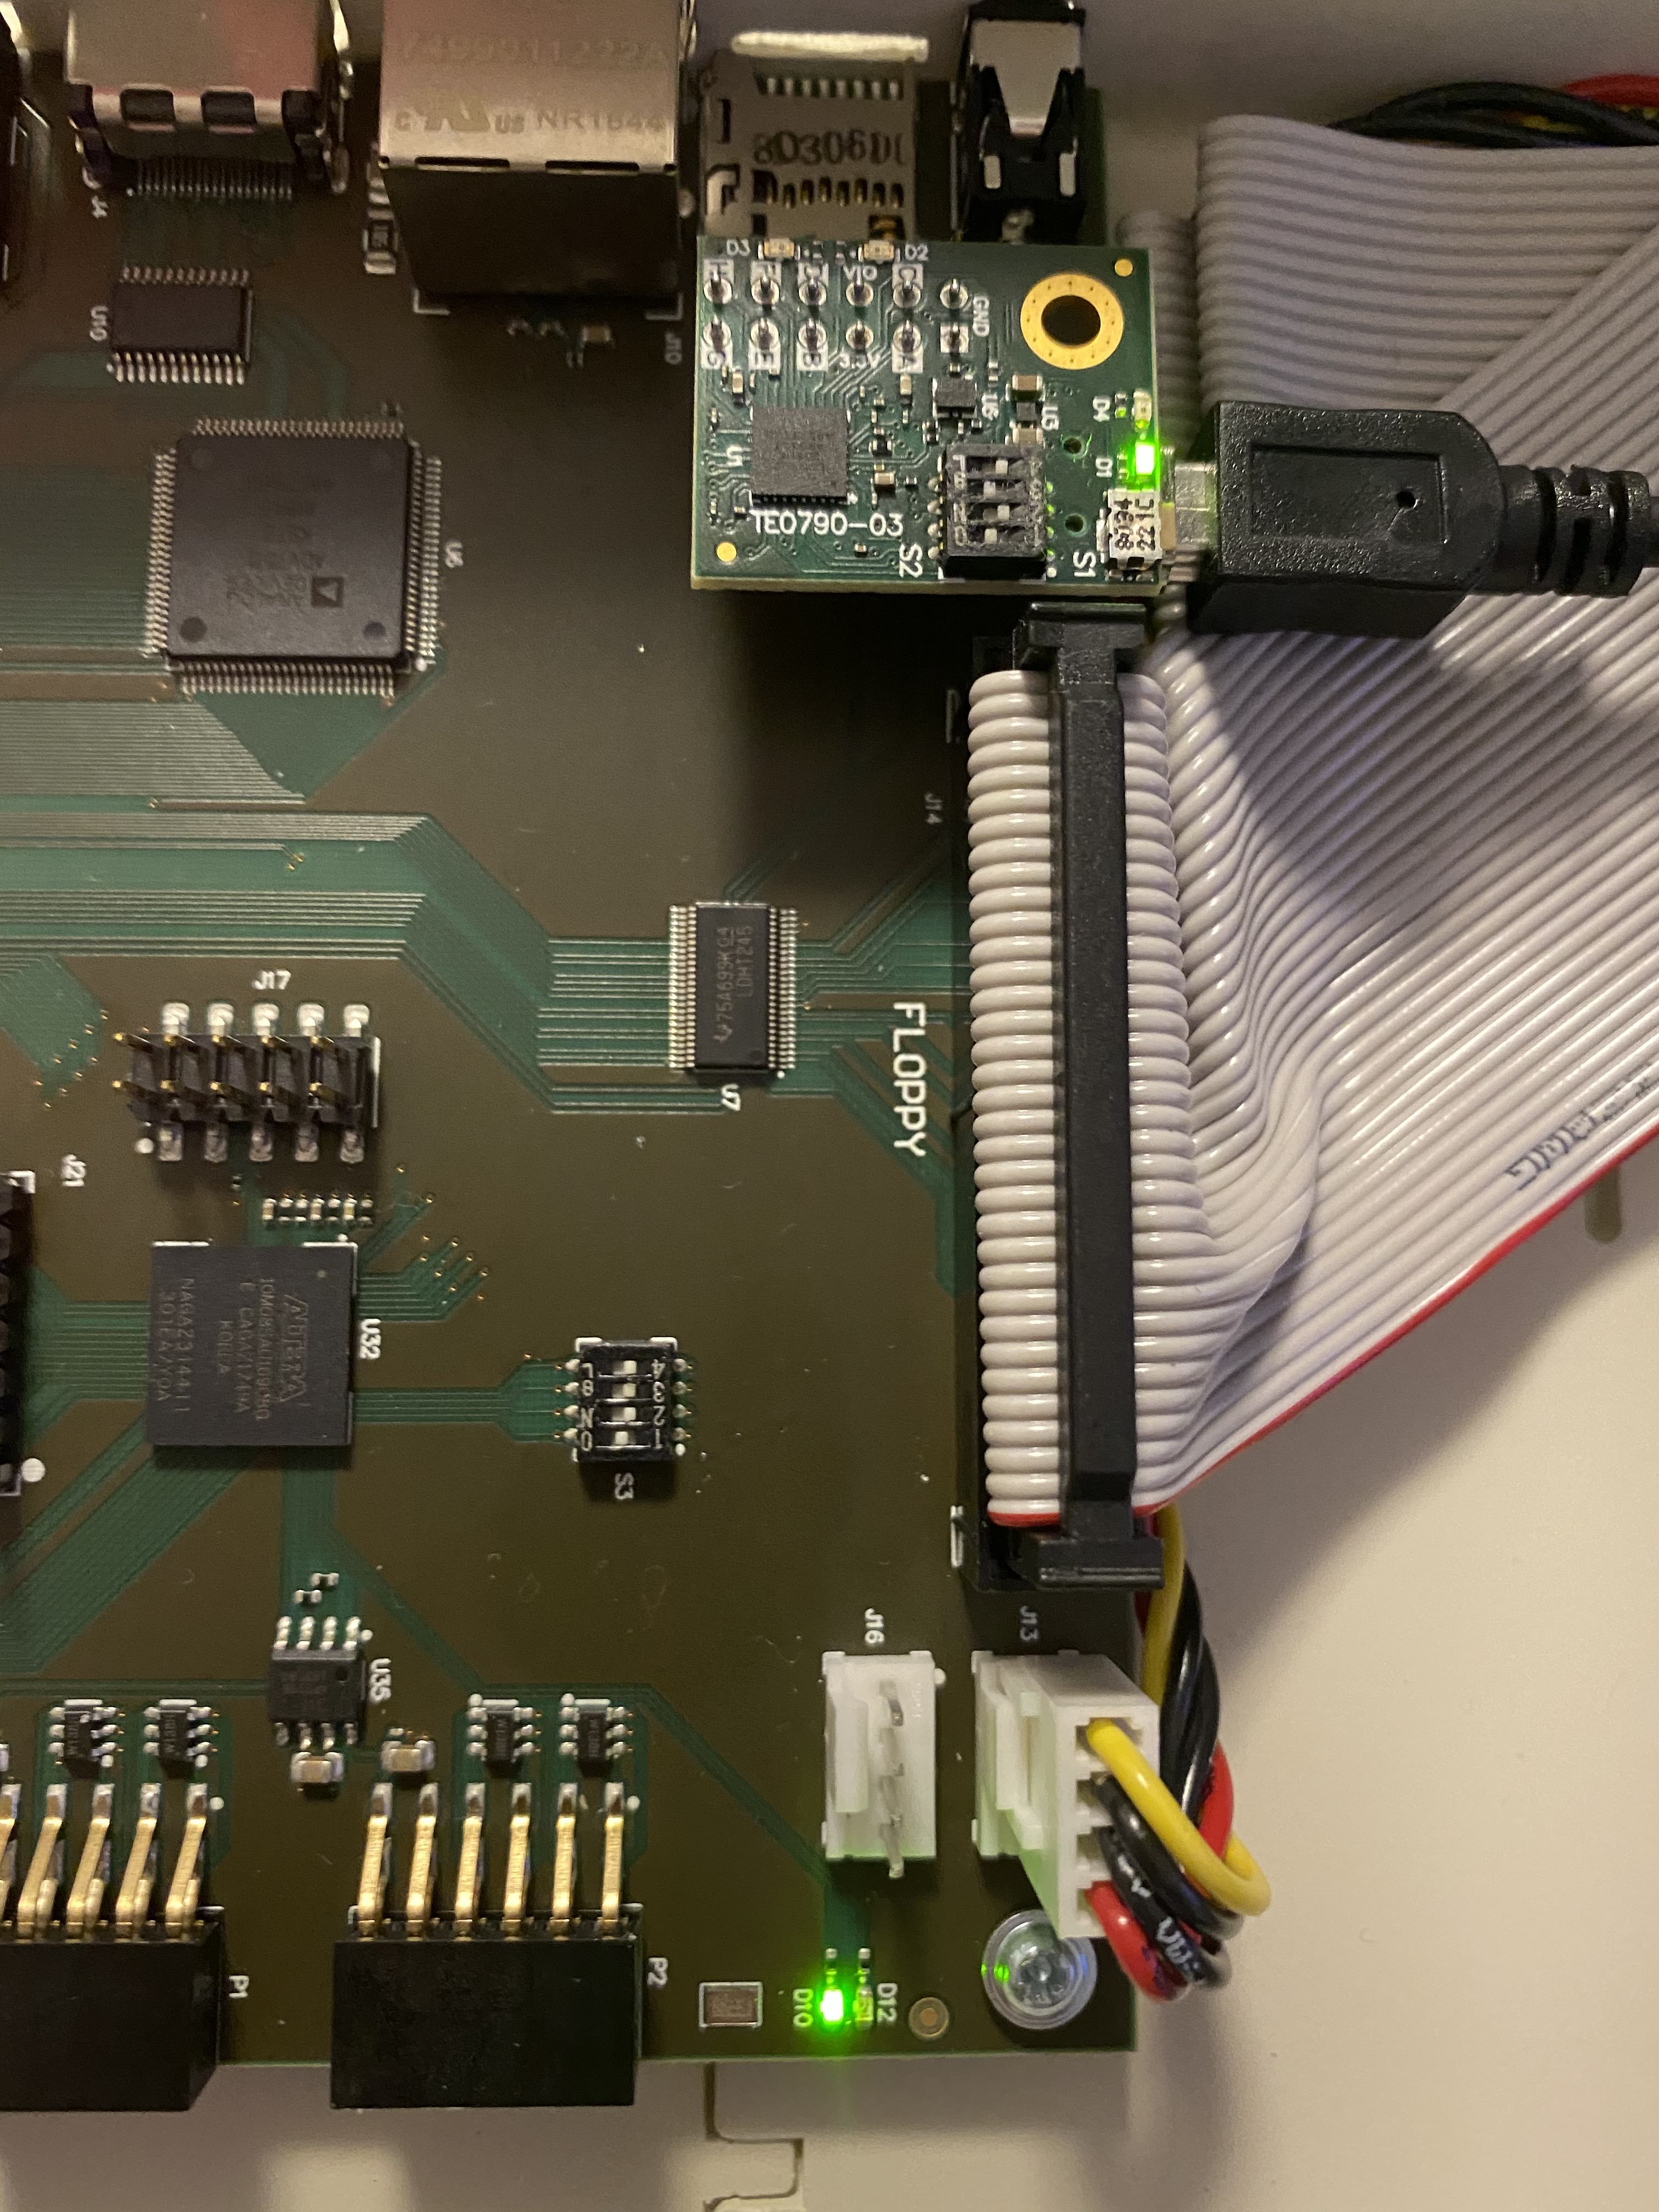
\includegraphics[width=\linewidth]{images/jtag_detail_05.jpg}


Op de PCB van een R2/R3/R3A/R4 MEGA65-moederbord moet dip-schakelaar 1 (de dichtstbijzijnde bij de gebruiker die voor de computer zit) op de AAN-stand staan. De overige schakelaars moeten UIT staan. Het toetsenbord gaat in de ``ambulance-modus'' (blauwe flitsende lichten) wanneer het correct is ingesteld.

Sluit uw niet-8-bit computer aan op het FPGA-programmeerapparaat met behulp van een mini-USB-kabel. Schakel de MEGA65-computer in. Open de Diamond Programmer, die van het internet kan worden gedownload.

\begin{minipage}{\linewidth}
Stap 1: Open DIAMOND PROGRAMMER: \\Selecteer ``Create a new project from a JTAG scan''. Indien het veld onder ``Cable:'' leeg is, klikt u op ``Detect Cable''.
\\
  \begin{center}
  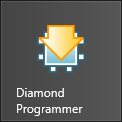
\includegraphics{images/diamond01.png}
  \end{center}
\end{minipage}

\vspace{5mm}

\begin{minipage}{\linewidth}
Stap 2: Maak een nieuw project aan: \\Indien het dialoogvenster ``Programmer: Multiple Cables Detected'' verschijnt, selecteert u het eerste item (``Location 0000'') en klikt u op ``OK''.
  \begin{center}
  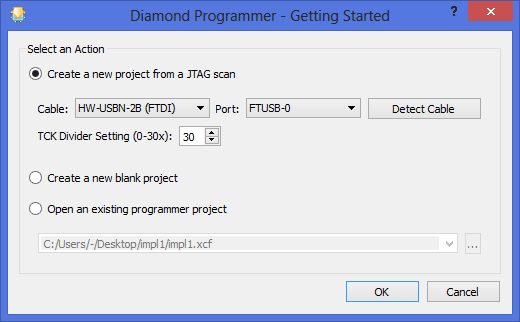
\includegraphics[width=0.7\linewidth]{images/diamond02.png}
  \end{center}
\end{minipage}


\begin{minipage}{\linewidth}
Stap 3: Selecteer kabel: \\U heeft nu een nieuw project aangemaakt dat ``MachXO2'' onder ``Device Family'' en ``LCMXO2-1200HC'' onder ``Device'' zou moeten weergeven.
  \begin{center}
  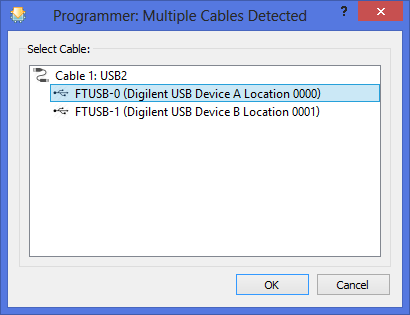
\includegraphics[width=0.6\linewidth]{images/diamond03.png}
  \end{center}
\end{minipage}

\vspace{5mm}

\begin{minipage}{\linewidth}
Stap 4: Nieuw Diamond Programmer-project: \\Kies ``File'' en vervolgens ``Open File'' om het Diamond Programmer-project met de firmware-update voor het MEGA65-toetsenbord te laden.
  \begin{center}
  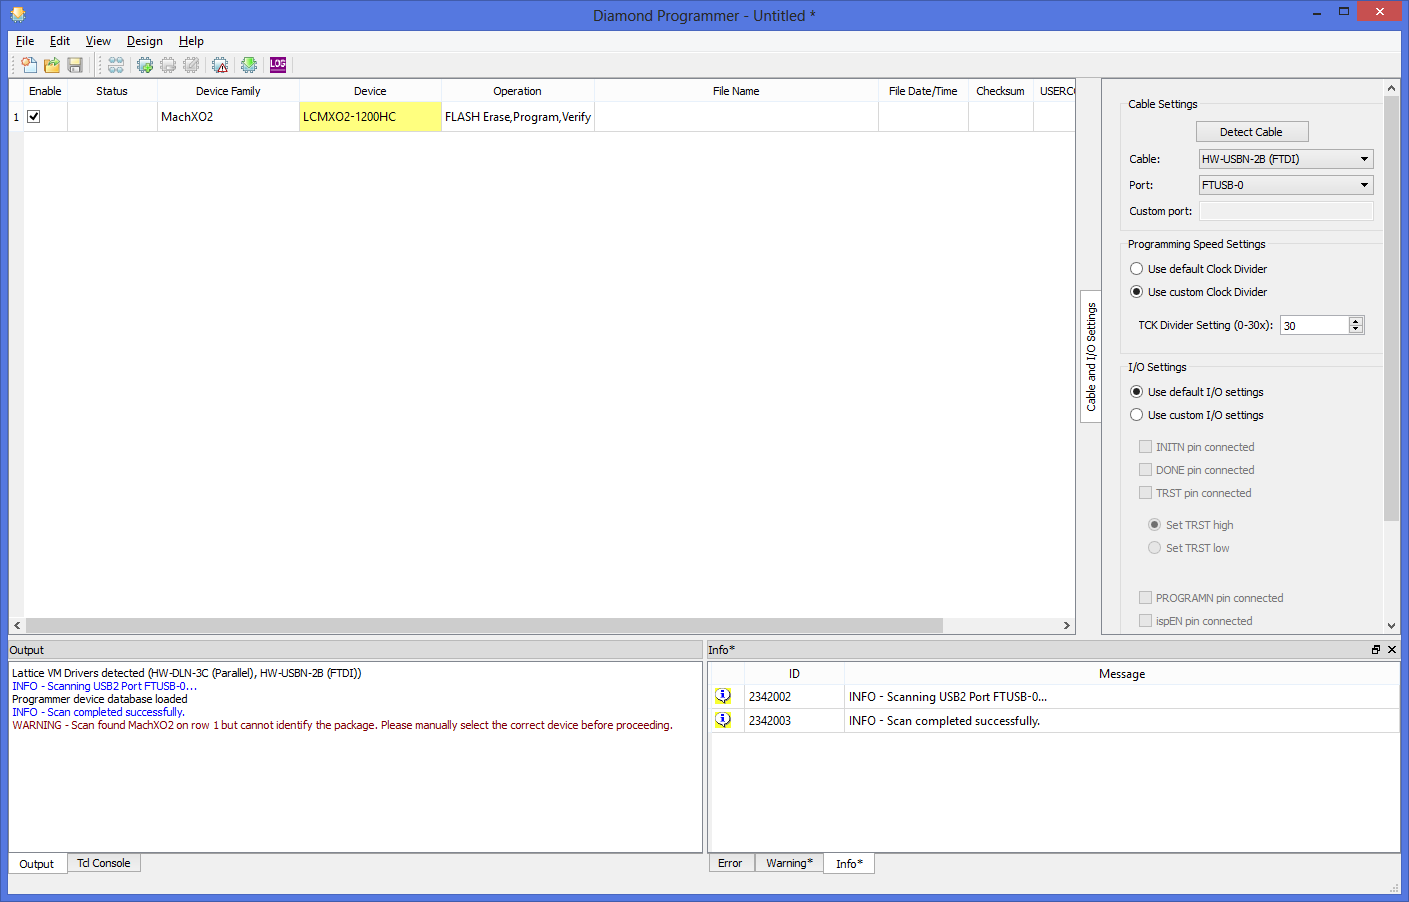
\includegraphics[width=0.8\linewidth]{images/diamond04.png}
  \end{center}
\end{minipage}


\begin{minipage}{\linewidth}
Stap 5: Open project: \\Navigeer naar de map met de uitgepakte firmwarebestanden voor het MEGA65-toetsenbord die u hebt ontvangen en selecteer het bestand met de extensie ``.xcf''.
  \begin{center}
  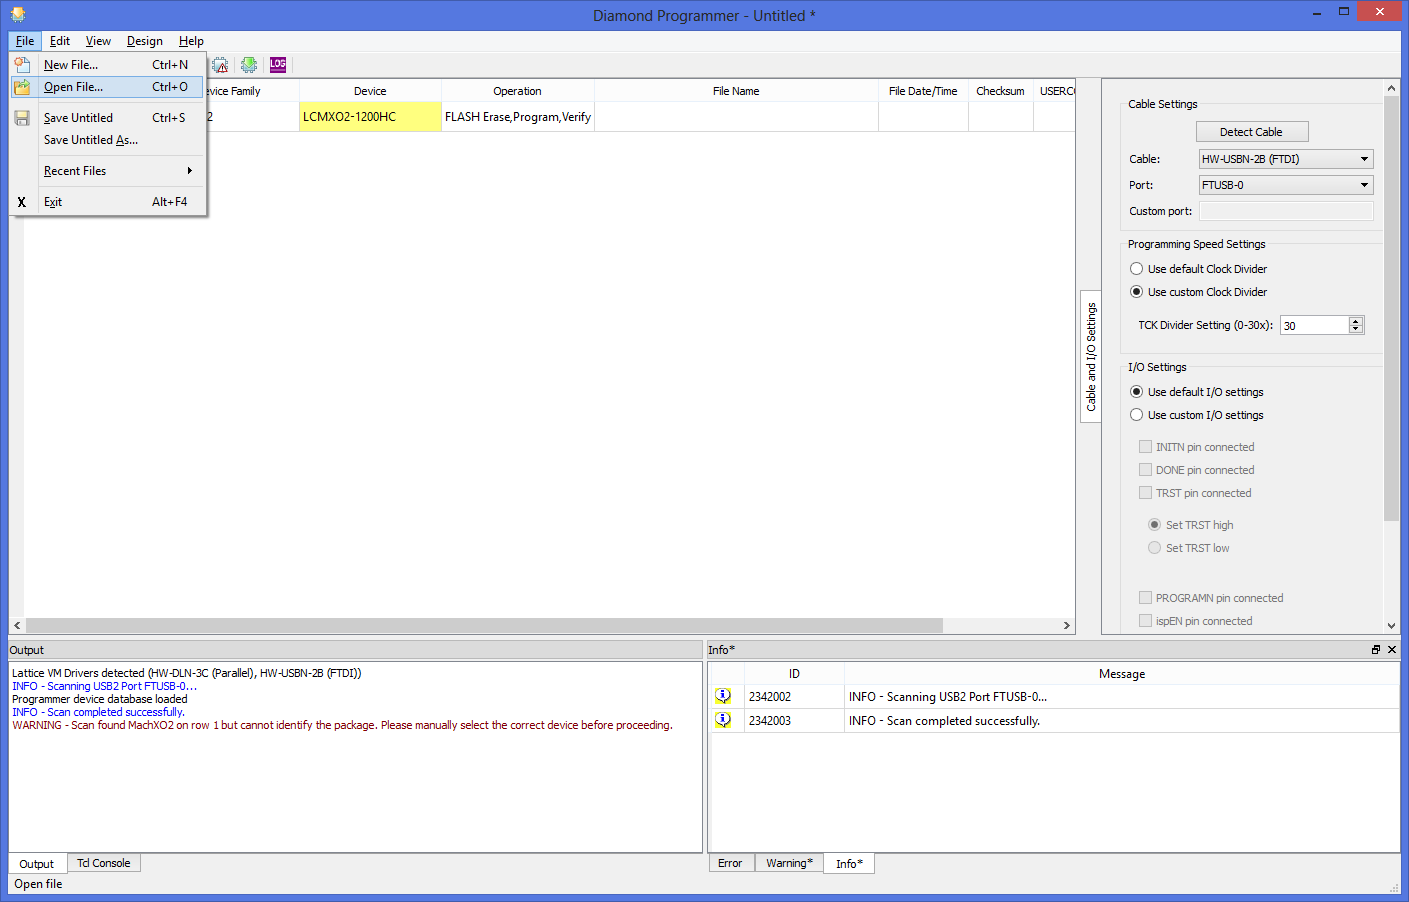
\includegraphics[width=0.8\linewidth]{images/diamond05.png}
  \end{center}
\end{minipage}

\vspace{5mm}

\begin{minipage}{\linewidth}
Stap 6: Selecteer projectbestand: \\Klik op de drie puntjes onder ``File Name'' om het juiste pad in te stellen en het bestand met de extensie ``.jed'' te vinden.
  \begin{center}
  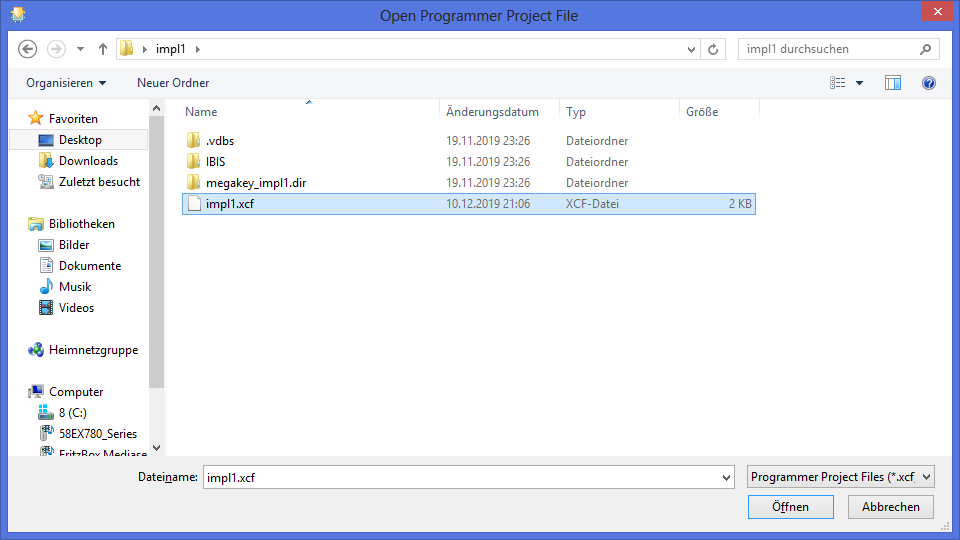
\includegraphics[width=0.8\linewidth]{images/diamond06.png}
  \end{center}
\end{minipage}


\begin{minipage}{\linewidth}
Stap 7: Kies het juiste pad van het .jed-bestand: \\Selecteer het bestand met de extensie ``.jed'' en klik op ``OK''.
  \begin{center}
  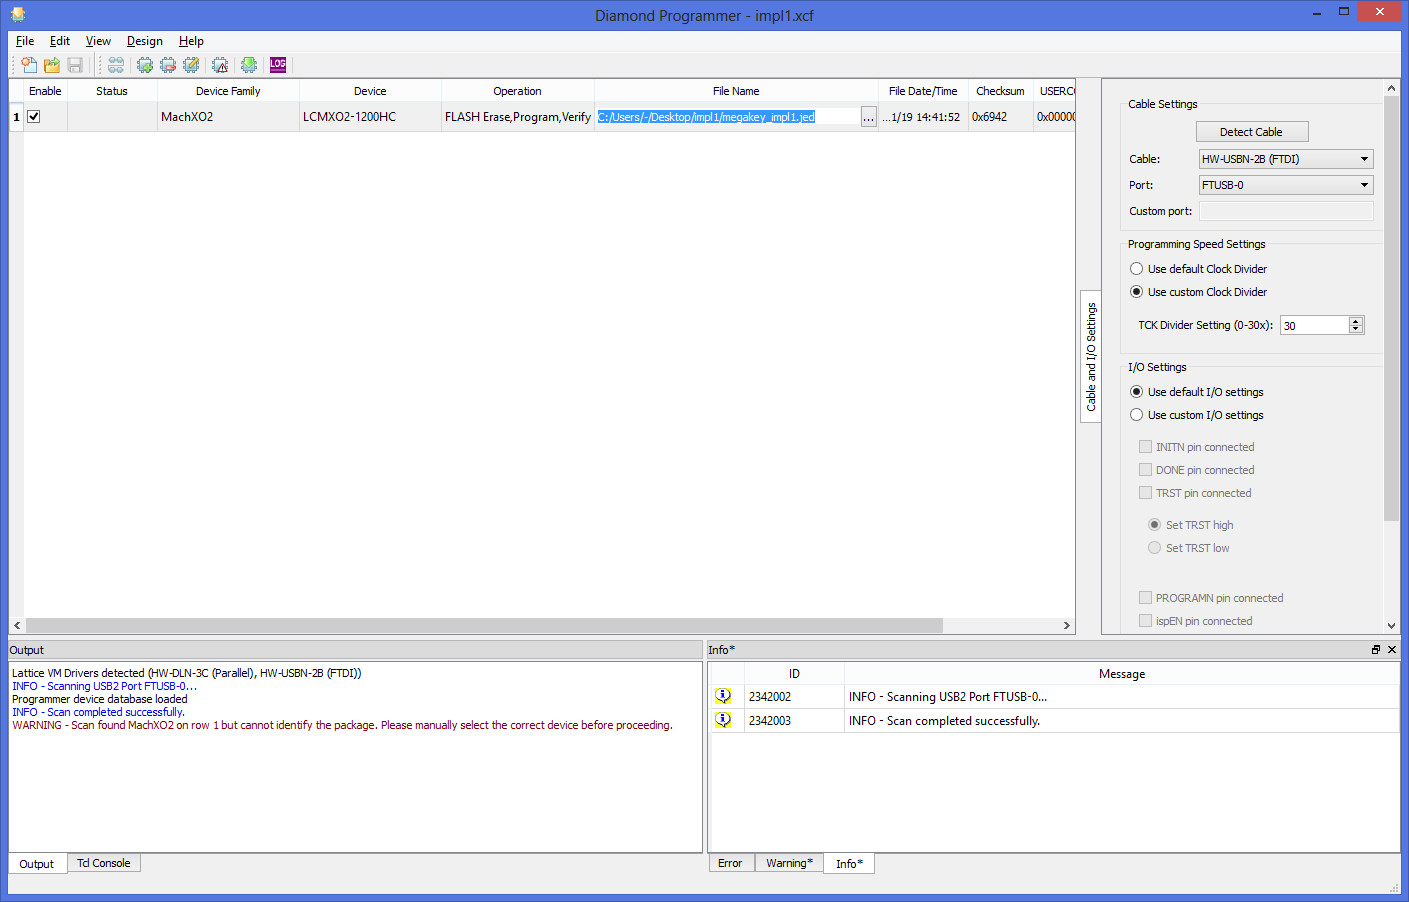
\includegraphics[width=0.8\linewidth]{images/diamond07.png}
  \end{center}
\end{minipage}

\vspace{5mm}

\begin{minipage}{\linewidth}
Stap 8: Selecteer .jed-bestand: \\Klik op het icoon met de groene pijl naar beneden ``PROGRAM'', dat lijkt op het icoon van het Diamond Programmer-programma.
  \begin{center}
  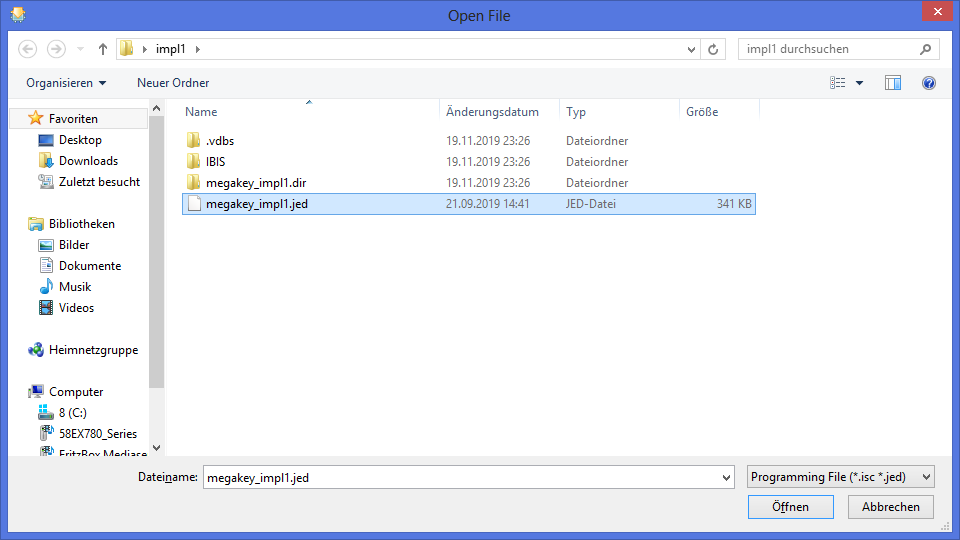
\includegraphics[width=0.8\linewidth]{images/diamond08.png}
  \end{center}
\end{minipage}


\begin{minipage}{\linewidth}
Stap 9: Selecteer kabel: \\Na een moment zou het uitvoervenster ``INFO - Operation: successful.'' moeten weergeven en zou het celletje ``Status'' groen moeten worden (dit gebeurt niet altijd).
  \begin{center}
  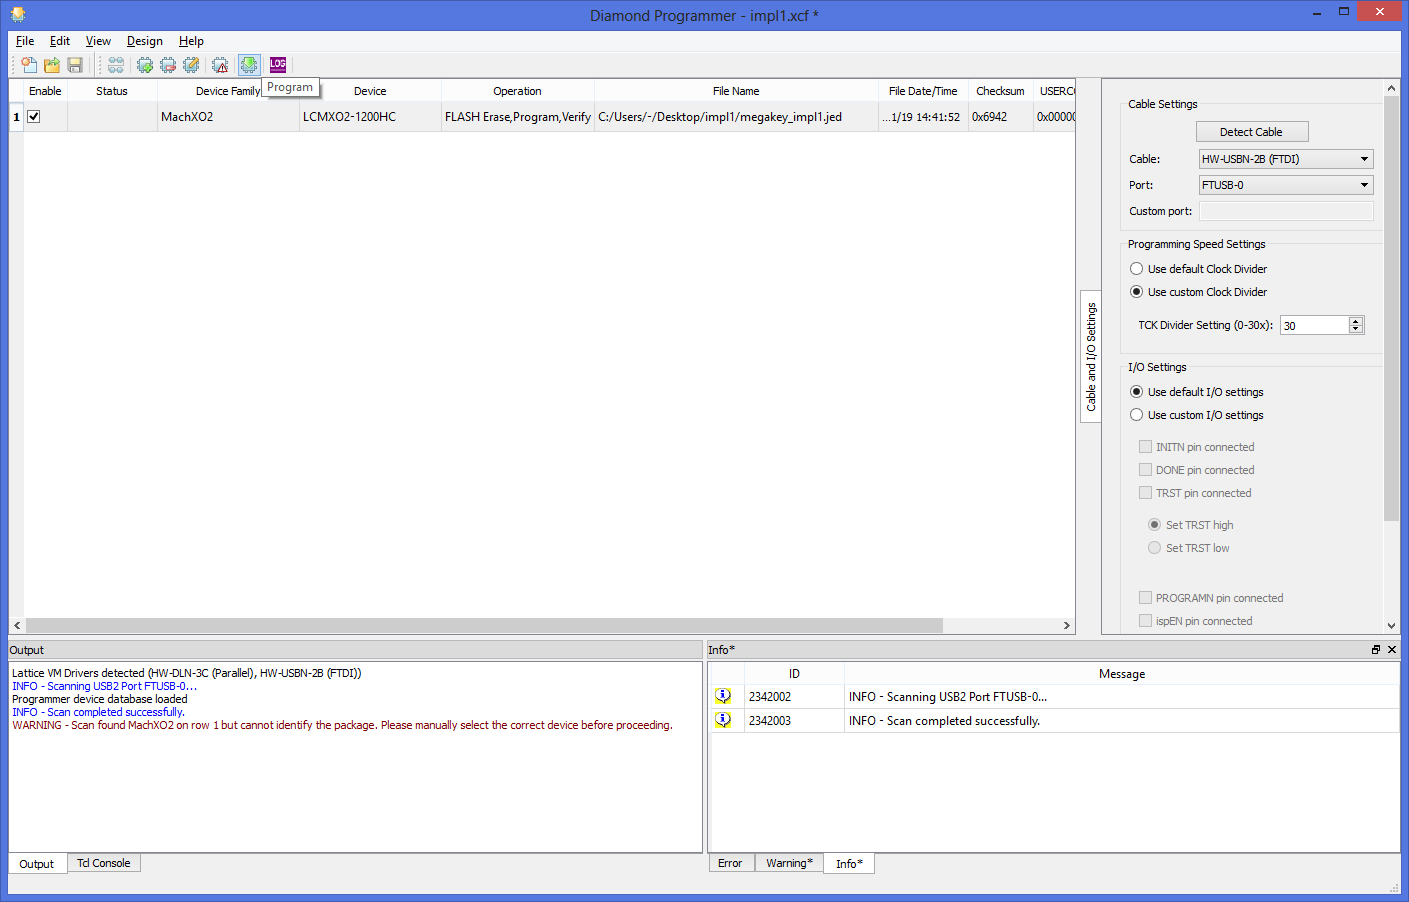
\includegraphics[width=0.8\linewidth]{images/diamond09.png}
  \end{center}
\end{minipage}

\vspace{5mm}

\begin{minipage}{\linewidth}
Stap 10: Operatie geslaagd: \\U heeft het MEGA65-toetsenbord nu succesvol geflasht. Desgewenst kunt u het project opslaan voor later gebruik.
  \begin{center}
  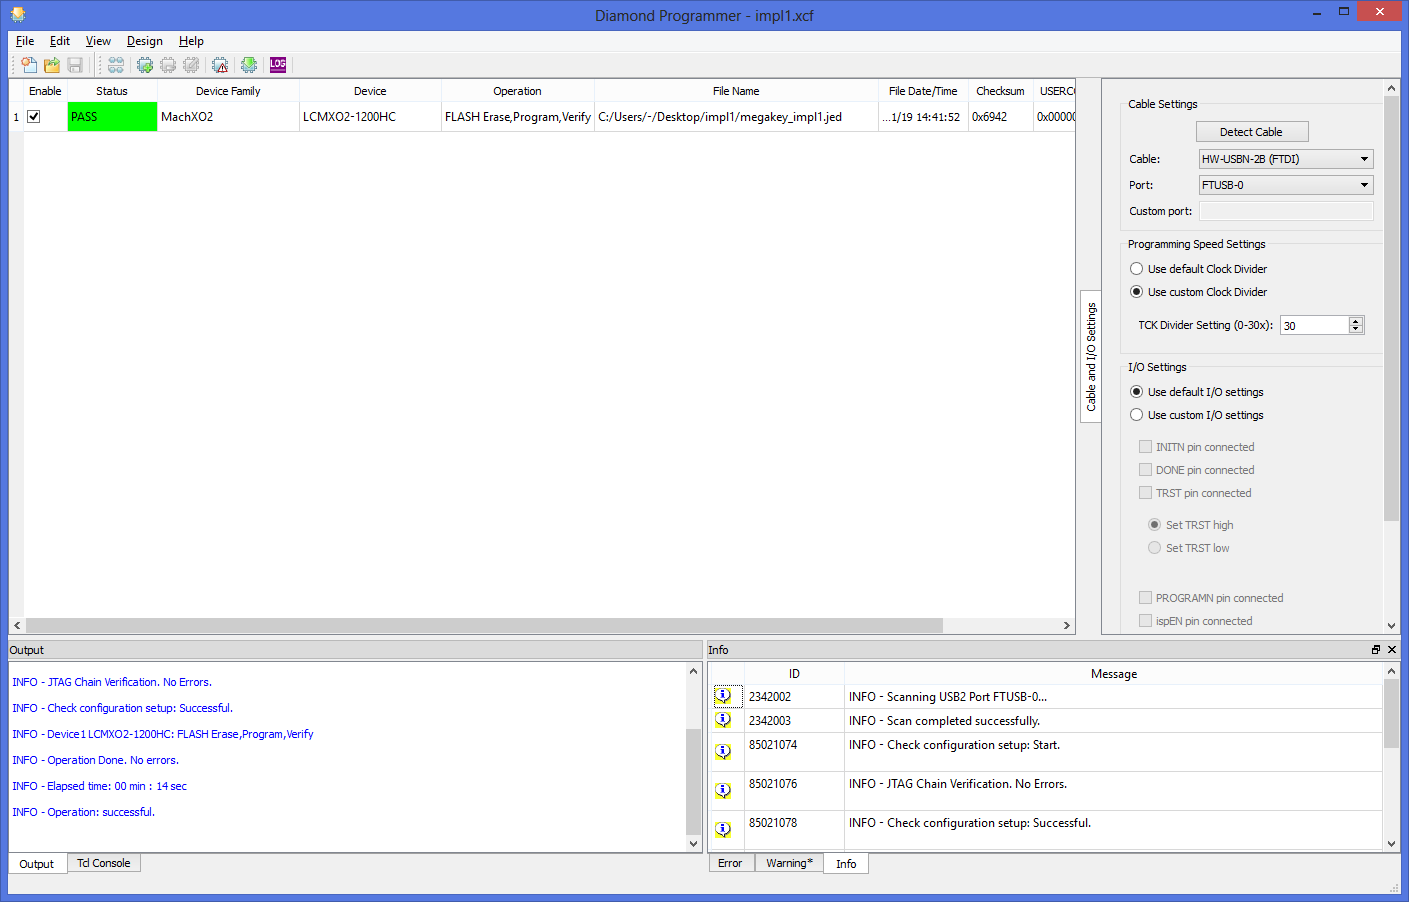
\includegraphics[width=0.8\linewidth]{images/diamond10.png}
  \end{center}
\end{minipage}


\section{Het flashen van de MAX10-FPGA op het MEGA65-moederbord met INTEL QUARTUS}
\label{sec:flashmax10}

Indien u verder wilt gaan, heeft u een TEI0004 - Arrow USB Programmer2-module nodig met het bijbehorende TEI0004-stuurprogramma geïnstalleerd en een goed functionerende installatie van Quartus Prime Programmer Lite Edition. Dit kan zowel op Windows als op Linux, maar in beide gevallen moet u de nodige USB-stuurprogramma's installeren. Sluit de MEGA65 niet aan op de netspanning en installeer de TEI0004 op de J17-connector, die zich tussen de datakabel van de diskette en de ARTIX 7-FPGA op het moederbord bevindt. De micro-USB-poort van de TEI0004 wijst in de tegenovergestelde richting van de HDMI- en LAN-aansluitingen, naar het klepje. De volgende afbeelding toont de juiste positie.

Op het PCB van een R2/R3/R3A/R4-MEGA65-moederbord moeten alle dip-schakelaars in de positie uit staan. De hoofd-FPGA van de MEGA65 mag geen geldige bitstream bevatten. De eenvoudigste manier om dit te bereiken is met een TE0790-JTAG-adapter: u kunt dan het m65-hulpprogramma vanaf een aangesloten computer gebruiken om een bitstream via JTAG te verzenden en vervolgens Control-C gebruiken om het m65-hulpprogramma te onderbreken voordat de bitstream volledig is geladen.

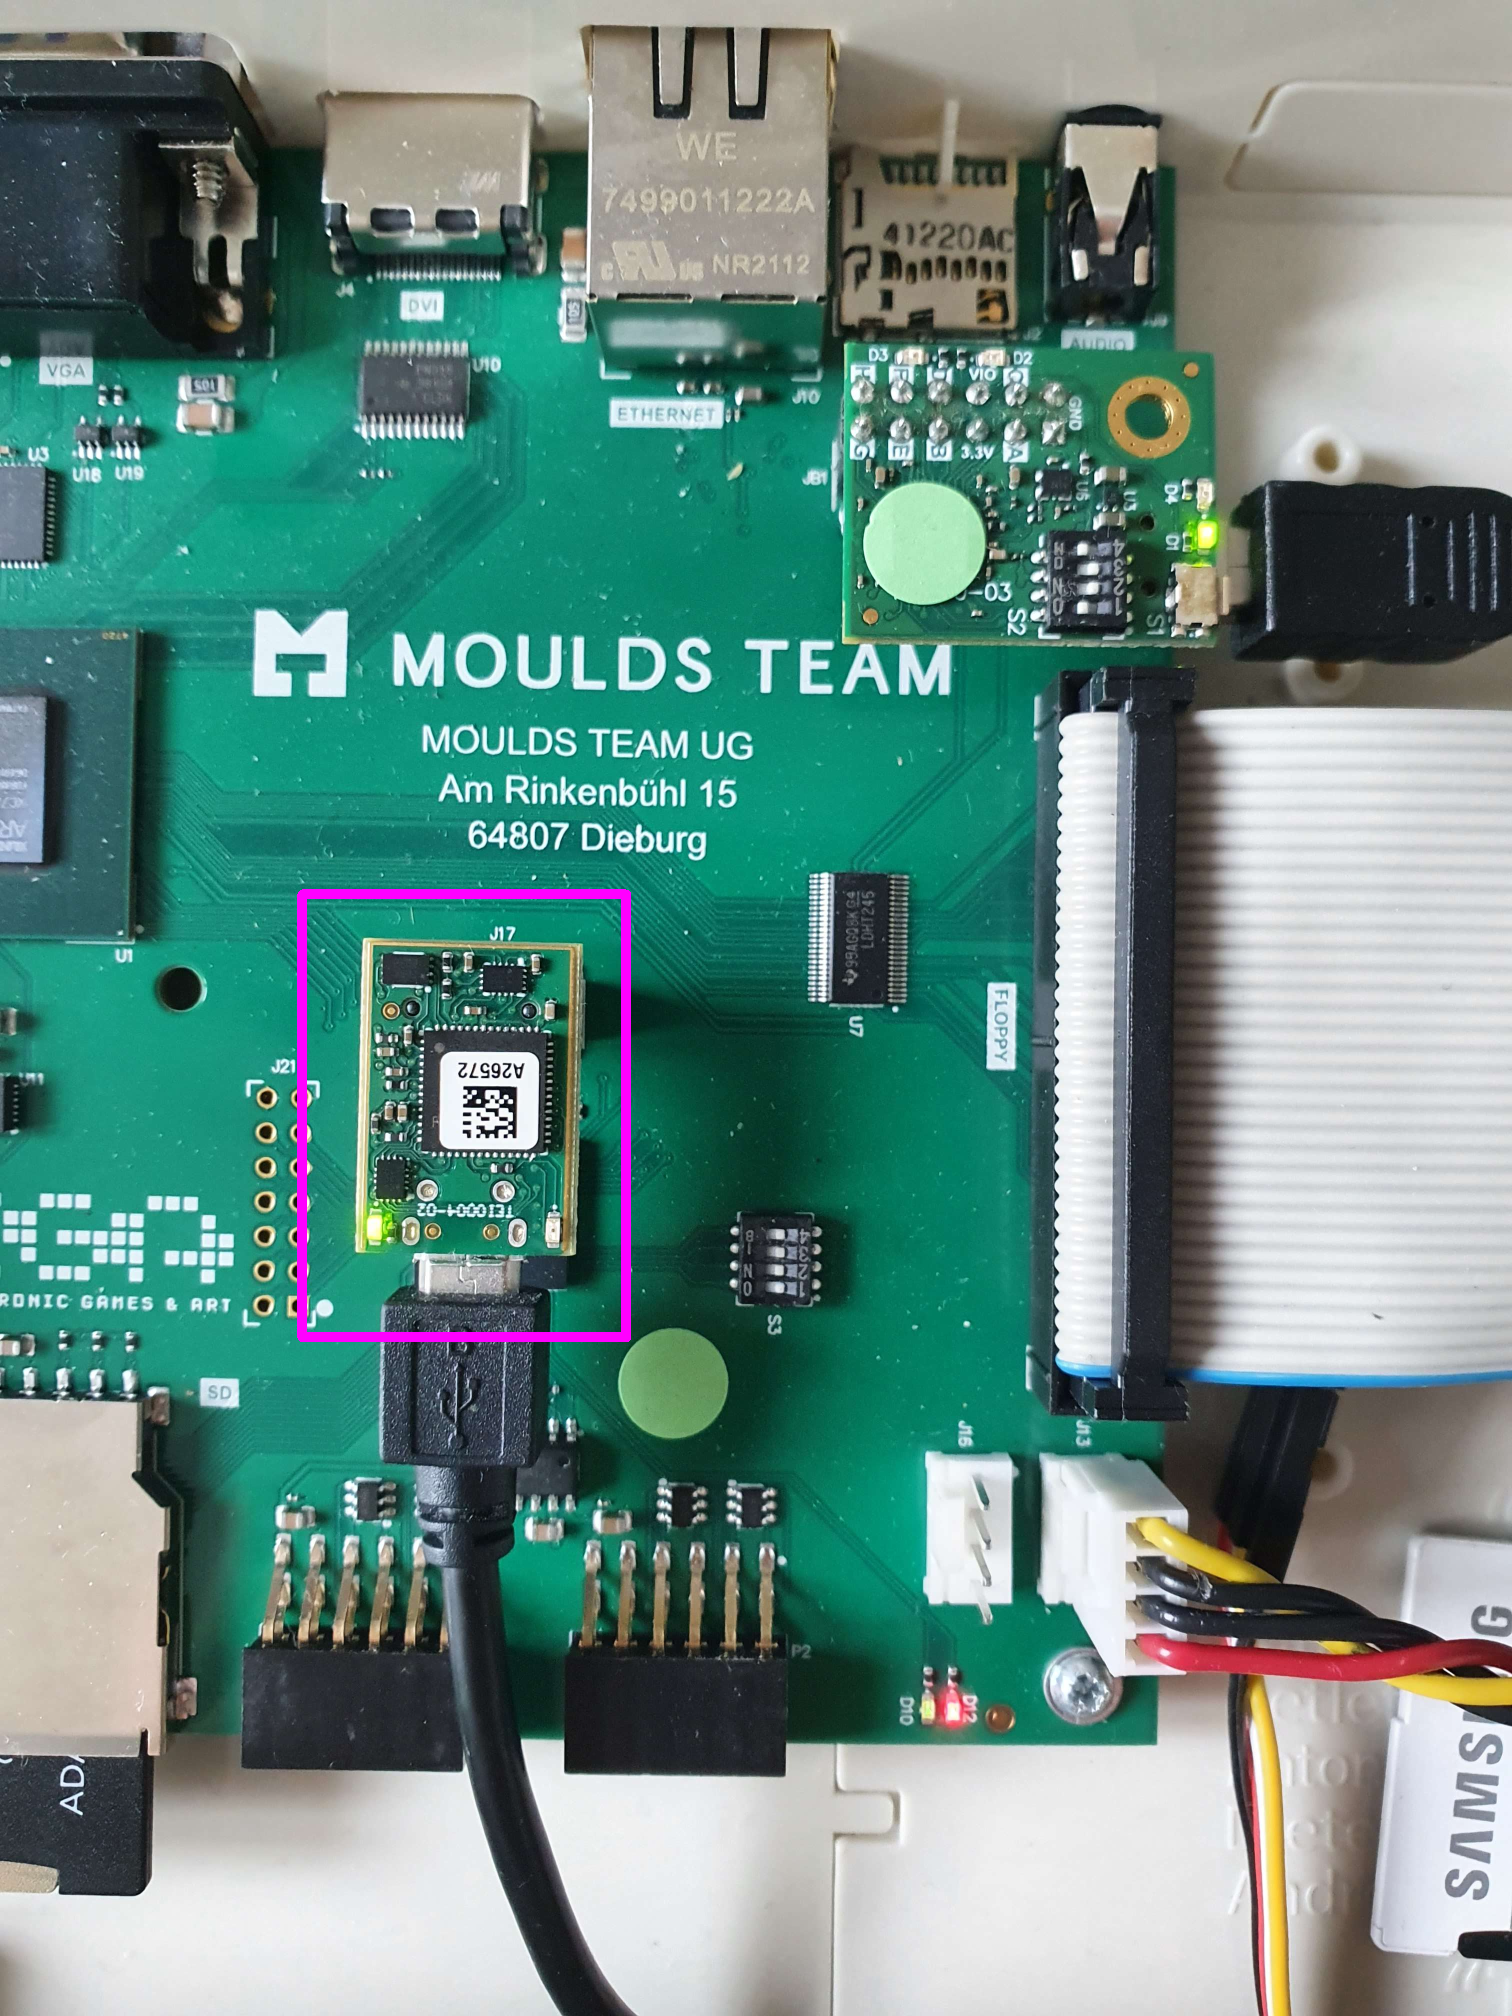
\includegraphics[width=\linewidth]{images/jtag_detail_max10.png}

Sluit uw niet-8-bit computer aan op het FPGA-programmeerapparaat met behulp van een micro-USB-kabel. Open Quartus Prime Programmer Lite Edition, dat van internet kan worden gedownload.

\begin{minipage}{\linewidth}
Stap 1: Open Quartus Prime Programmer Lite Edition: \\Klik op de knop ``Hardware Setup'' in de linkerbovenhoek van het Quartus Prime Programmer-venster.
  \begin{center}
  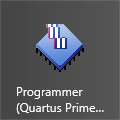
\includegraphics{images/max10_01.png}
  \end{center}
\end{minipage}

\vspace{5mm}

\begin{minipage}{\linewidth}
Stap 2: Hardware-instellingen invoeren: \\In het nieuw verschenen venster kiest u onder ``Currently selected hardware'' voor ``Arrow-USB-Blaster''. Indien ``Arrow-USB-Blaster'' niet verschijnt, controleert u of de kabel en stuurprogramma's correct zijn geïnstalleerd.
  \begin{center}
  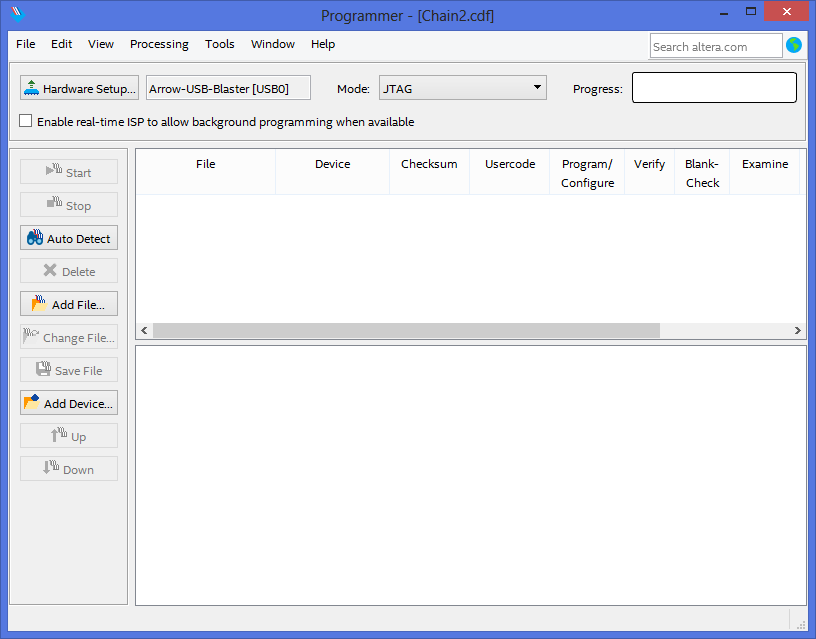
\includegraphics[width=0.8\linewidth]{images/max10_02.png}
  \end{center}
\end{minipage}


\begin{minipage}{\linewidth}
Stap 3: Selecteer Arrow USB-Blaster: \\Klik op de knop ``Add File'' in de linkerrij en kies het nieuwste bestand met de extensie ``.pof''. Klik vervolgens op ``Open''.
  \begin{center}
  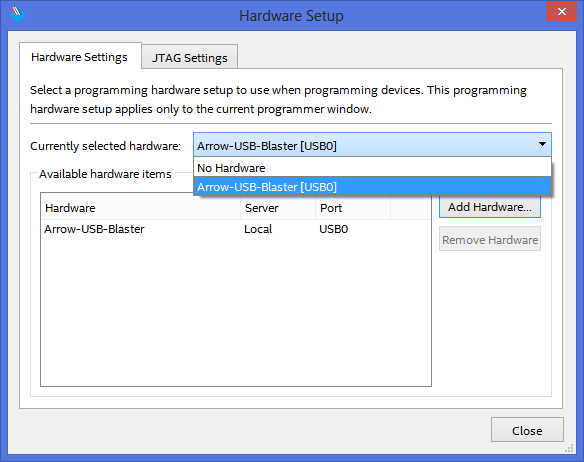
\includegraphics[width=0.8\linewidth]{images/max10_03.png}
  \end{center}
\end{minipage}


\begin{minipage}{\linewidth}
Stap 4: Selecteer programmeerbestand: \\Vink ten minste de drie vakjes onder ``Program/Configure'' aan. Het inschakelen van alle vakjes onder ``Verify'' en ``Blank-Check'' maakt het proces betrouwbaarder.
  \begin{center}
  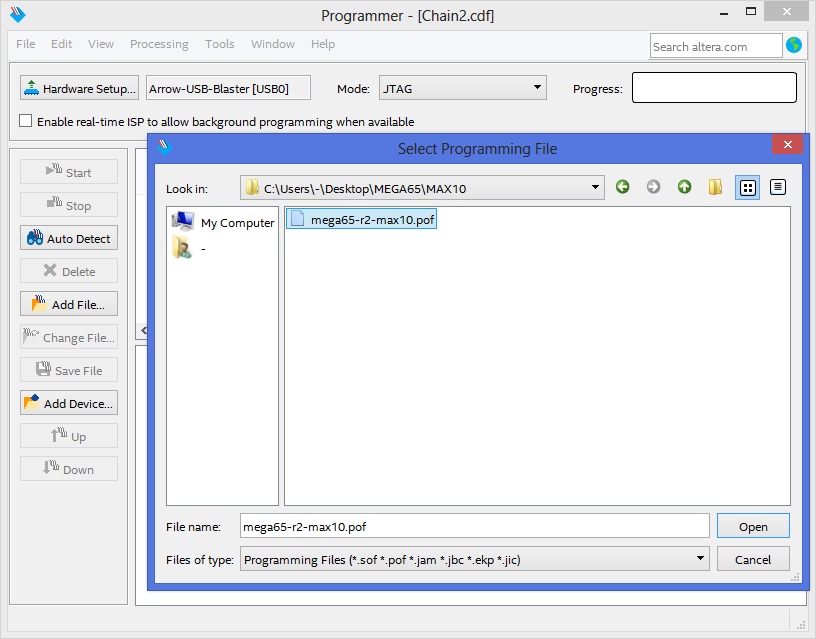
\includegraphics[width=0.7\linewidth]{images/max10_04.png}
  \end{center}
\end{minipage}

\vspace{5mm}

\begin{minipage}{\linewidth}
Stap 5: Selecteer Programmeer-/Configureeropties:
  \begin{center}
  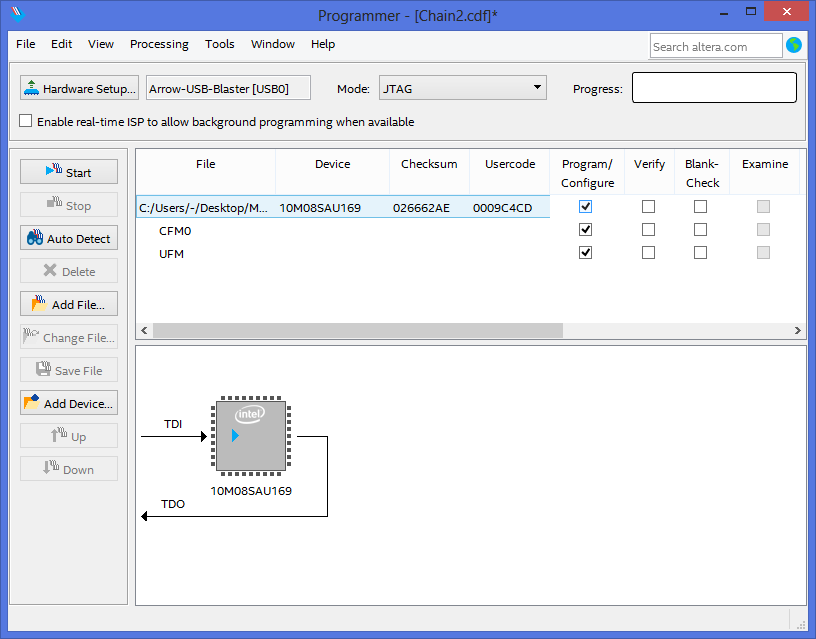
\includegraphics[width=0.7\linewidth]{images/max10_05.png}
  \end{center}
\end{minipage}

Houd de Reset-knop ingedrukt en schakel de MEGA65-computer in. Het toetsenbord gaat in de ``ambulance mode'' (blauwe flitsende lichten). Indien dit niet het geval is, is de hoofd-FPGA niet leeg: start het gehele proces opnieuw.

Klik nu op ``Start'' in de linkerrij van knoppen. De voortgangsbalk rechtsboven zou snel naar 100 procent moeten gaan en groen moeten worden. U heeft de MAX10-FPGA nu succesvol bijgewerkt.

Indien u in plaats daarvan een foutmelding ontvangt, controleer dan of de bitstream van de hoofd-FPGA is gewist en of u de reset-knop op de MEGA65 niet te vroeg heeft losgelaten. Schakel de MEGA65 uit en herhaal deze stap.

\begin{minipage}{\linewidth}
Stap 6: Programmeren geslaagd:
  \begin{center}
  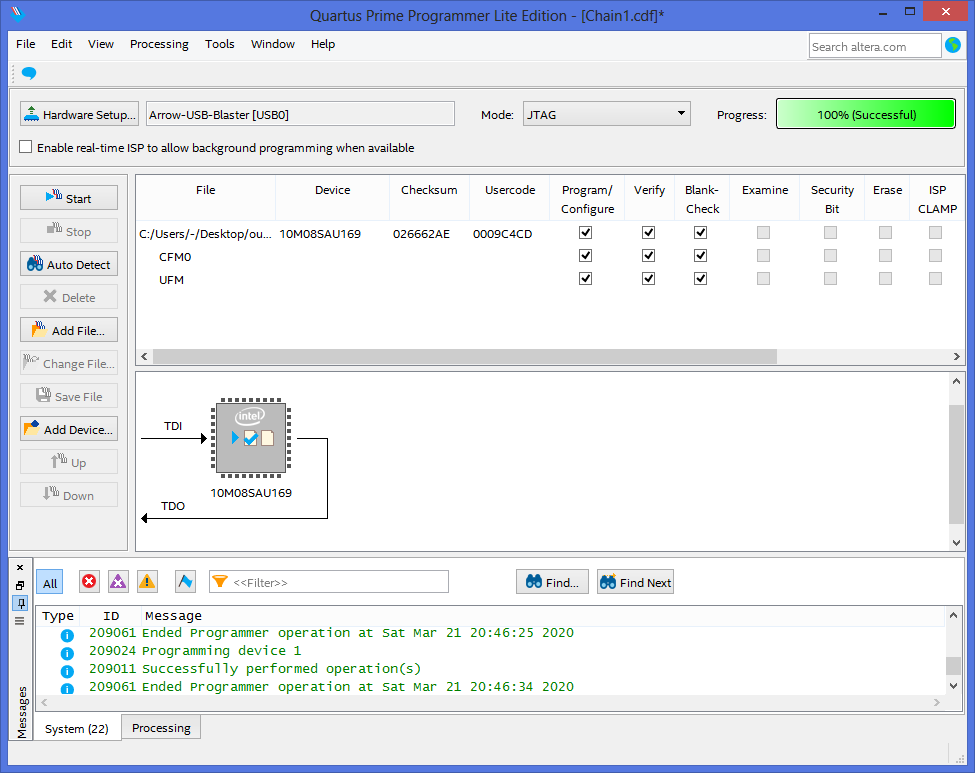
\includegraphics[width=0.8\linewidth]{images/max10_06.png}
  \end{center}
\end{minipage}


  \lstset{
    basicstyle=\small\ttfamily,    columns=flexible,    breaklines=true
}

\chapter{Problemen oplossen}

\section{Hardware}
    \subsection{Geen digitale video-uitvoer}

    \subsubsection{MEGA65 R4, R5, R6}
    De digitale videopoort heeft een verbeterde isolatie tegen terugvoeding gekregen om het probleem ``Geen lampjes bij het inschakelen'' op te lossen.  Een neveneffect hiervan is dat sommige digitale videokabels ten onrechte alleen de behuizing van de connector gebruiken om het grondsignaal door te geven, in plaats van de grondsignalen van de pinnen van de connector te gebruiken.  Kort samengevat: als u geen beeld krijgt op de digitale videopoort, kunt u een van de volgende oplossingen proberen:
    \begin{itemize}
    \item Probeer verschillende digitale videokabels die u heeft.  Dit probleem komt alleen voor bij bepaalde merken kabels, vooral dunnere exemplaren, waarvan wij sterk vermoeden dat de interne grondleidingen ontbreken om kosten te besparen. Dit is de beste oplossing, omdat de kabel daadwerkelijk de oorzaak van het probleem is doordat deze niet aan de specificaties voldoet. Zelfs als u een van de volgende oplossingen toepast, moet u toch op zoek gaan naar een betere HDMI-kabel die het probleem bij de bron oplost.    \item Sluit een VGA-kabel aan op de MEGA65 en op hetzelfde beeldscherm. Hierdoor wordt een grondverbinding via de VGA-connector tot stand gebracht, waardoor de HDMI op mysterieuze wijze plotseling lijkt te werken.    \item Sluit een TE0790 JTAG-adapter aan. Een gebruiker meldde dat dit het probleem eveneens op mysterieuze wijze omzeilde.    \item Verbind de behuizing van de digitale video-connector met de behuizing van de interne SD-kaart op vol formaat.    \item Sluit een splitter of repeater aan op de digitale videopoort.
    \end{itemize}

\begin{figure}
\label{baddvicable}
\caption{Voorbeeld van een slechte (boven) en goede (onder) digitale videokabel. Let op hoe de slechte kabel verdacht dunner is dan de goede. Dit is een teken dat waarschijnlijk dedicated grondleidingen ontbreken, wat problemen veroorzaakt op de MEGA65 R4 en latere revisies.  Elke kabel van ``normale dikte'' zou echter goed moeten werken.  U hoeft geen van die peperdure ``met zilverdraad gevlochten, bij maanlicht door elfen gesmeede'' kabels te kopen.  Die kabels bieden ongeveer evenveel praktisch nut als het strooien van glitter of het tekenen van een eenhoorn aan één uiteinde, maar dan met veel minder klasse.}
\centering
 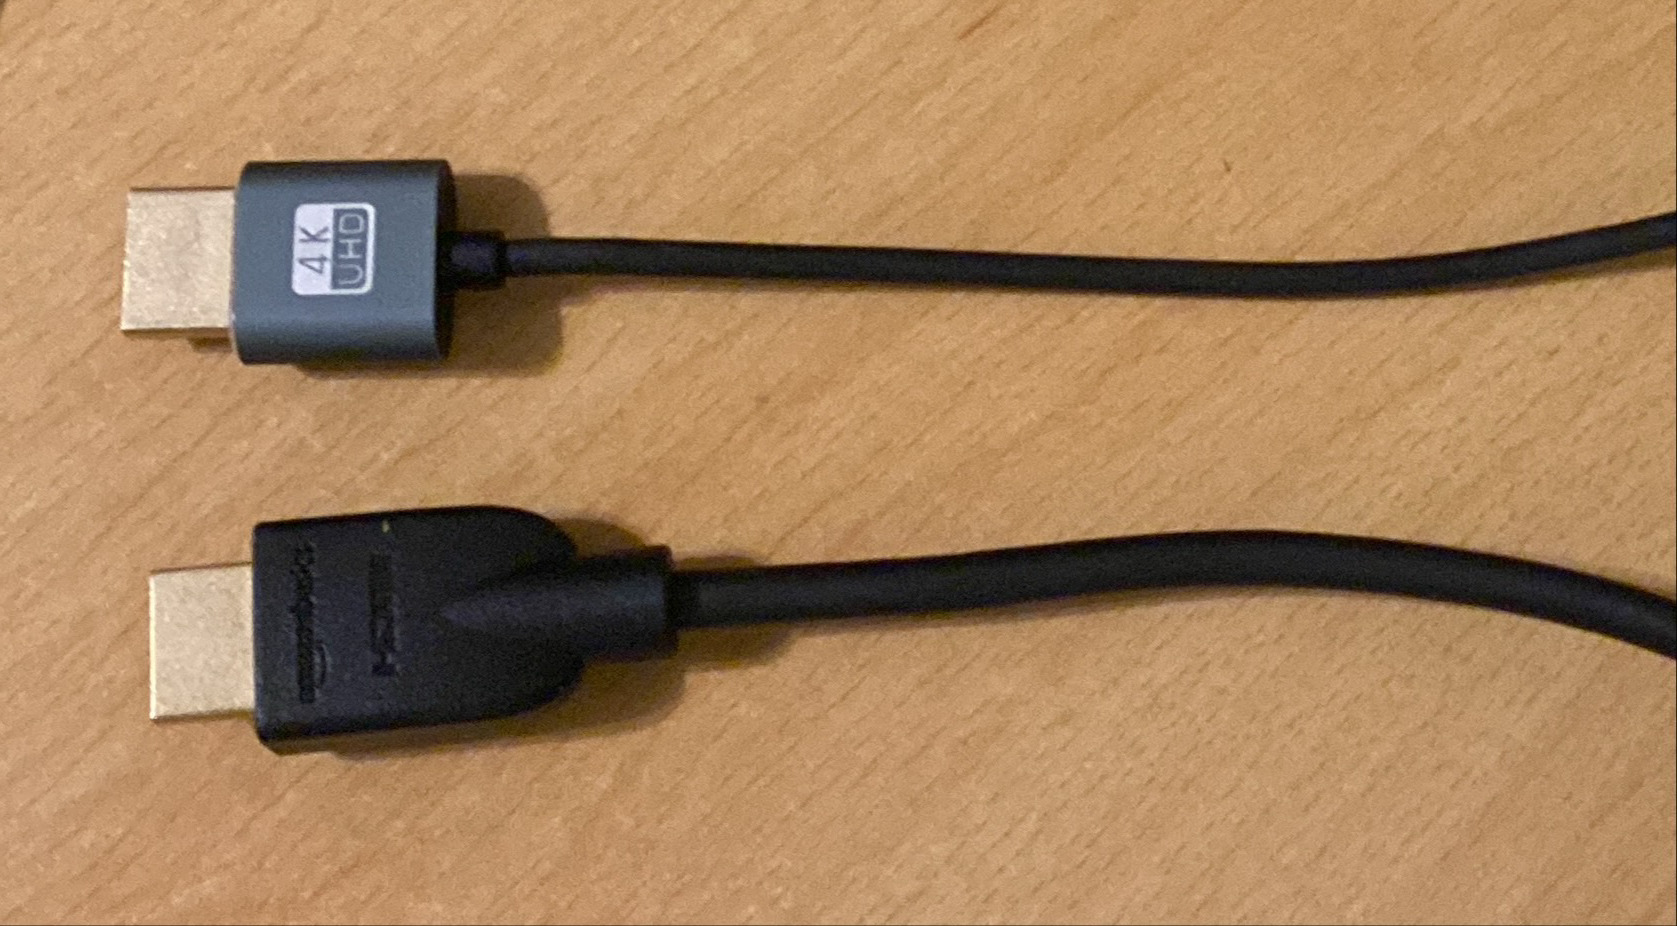
\includegraphics[width=0.7\linewidth]{images/bad-and-good-video-cables.jpg}
\end{figure}

    \subsection{Geen lampjes bij het inschakelen}
    Als de MEGA65 bij het inschakelen soms geen lampjes laat zien, heeft dit te maken met bepaalde digitale video-apparaten die op het moment dat de MEGA65 uitstaat aangesloten zijn en onvoldoende vermogen leveren om de CPLD van het toetsenbord correct van stroom te voorzien, maar wel genoeg om te voorkomen dat deze goed kan resetten wanneer de MEGA65 wordt ingeschakeld. Het verwijderen van de digitale videokabel en het opnieuw inschakelen van het apparaat lost het probleem op.

\section{Vivado}
    \subsection{RAM-vereisten}
    \begin{tcolorbox}[colback=black,coltext=white]
    \begin{lstlisting}
INFO: [Synth 8-256] done synthesizing module 'ram32x1024' [/home/....]
INFO: [Synth 8-256] synthesizing module 'charrom' [/home/....]
    /opt/Xilinx/Vivado/2019.2/bin/loader: line 280: 2317 killed
    WARNING: [Vivado 12-8222] Failed run(s) : 'synth\_1'
        ERROR: Application Exception: failed to launch run 'impl\_1' due to failures in the following run(s):
        synth\_1
        These failed run(s) need to be reset prior to launching 'impl\_1' again.
    \end{lstlisting}
    \end{tcolorbox}
Deze fout wordt veroorzaakt doordat Vivado crasht omdat het apparaat onvoldoende RAM heeft om Vivado uit te voeren.  Vivado heeft minimaal 4 GB RAM nodig om het MEGA65-doel te synthetiseren, maar 8 GB is beter.

\section{mega65\_ftp}
    \subsection{Ontbrekende bibliotheek}
    \begin{tcolorbox}[colback=black,coltext=white]
\begin{lstlisting}
/usr/bin/ld: cannot find -lncurses
collect2: error: ld returned 1 exit status
Makefile:474: recipe for target 'bin/mega65_ftp' failed
make: *** [bin/mega65_ftp] Error 1\end{lstlisting}
    \end{tcolorbox}
Deze fout treedt op wanneer de ncurses-bibliotheek op de computer ontbreekt bij het bouwen van het mega65\_ftp-programma.
Om dit probleem op te lossen, moet u deze afhankelijkheid installeren.

    \begin{tcolorbox}[colback=black,coltext=white]
\begin{lstlisting}
sudo apt-get install libncurses5-dev libncursesw5-dev\end{lstlisting}
    \end{tcolorbox}


  \chapter{Modelspecifieke kenmerken}

\section{MEGA65-modellen detecteren}

Hoewel we verwachten dat de productieversie van de MEGA65 een stabiel platform is, kunnen er zich nog situaties voordoen waarin het nodig is vast te stellen op welke hardware uw programma draait. Dit is met name belangrijk voor de systeemsoftware van de MEGA65, welke mogelijk verschillende hardwareonderdelen op de verschillende modellen moet initialiseren. Omdat er al een handheld-versie van de MEGA65 in ontwikkeling is, welke een scherm met een iets andere resolutie gebruikt (800x480 in plaats van 720x576) en wel een touchscreen heeft, maar geen hardwaretoetsenbord. wilt u wellicht programma's maken die zich op een soepelere manier aan deze handheld-apparaten aanpassen. U kunt bijvoorbeeld touchscreeninvoer inschakelen en de keuzemogelijkheden op het scherm zo herindelen dat ze groot genoeg zijn om gemakkelijk met een vinger te activeren.

De eenvoudige manier om vast te stellen op welk model MEGA65 uw programma draait, is het controleren van het register \$D629 (schakel echter eerst de MEGA65-I/O-persoonlijkheid in, via \$D02F). Dit register bevat een 8-bits hardware-identificatie. De volgende waarden zijn momenteel gedefinieerd:

\begin{description}[align=left,labelwidth=0.2cm]
\item[\$01 (1)] MEGA65 R1\item[\$02 (2)] MEGA65 R2\item[\$03 (3)] MEGA65 R3\item[\$04 (4)] MEGA65 R4\item[\$05 -- \$0F (5 -- 15)] MEGA65 R5 -- MEGA65 R15\item[\$21 (33)] MEGAphone (handheld) R1\item[\$40 (64)] Nexys4 PSRAM\item[\$41 (65)] Nexys4DDR\item[\$42 (66)] Nexys4DDR met widget-bord\item[\$FD (253)] QMTECH Wukong A100T-bord\item[\$FE (254)] VHDL-simulatierun
\end{description}


\section{MEGA65-desktopcomputer, revisies 5 en 6}

De desktop-PCB's van R5 en R6 vormen betrekkelijk bescheiden herzieningen van de desktop-PCB van R4, die oorspronkelijk werd uitgevoerd om problemen met de toeleveringsketen voor enkele voedingsregelaarcomponenten op te lossen. Hierbij hebben de ontwerpers tevens de gelegenheid aangegrepen om enkele verbeteringen door te voeren:

\begin{itemize}
\item Enkele signalen op de uitbreidingspoort die voorheen alleen uitvoer of alleen invoer waren, zijn nu bidirectioneel, zodat de C64-core naar verwachting alle bekende cartridges kan ondersteunen en de cartridgecompatibiliteit van de MEGA65-core verder kan worden verbeterd.\item Op het moederbord zijn vier extra DIP-schakelaars toegevoegd. Alle acht DIP-schakelaars zijn nu aangesloten via een I2C-I/O-expander, in plaats van dat zij rechtstreeks FPGA-pinnen in beslag nemen.\item Deze nieuwe I/O-expander biedt tevens informatie over de major- en minorrevisie van het moederbord. De hoofdrevisie is ingesteld op 5 en de subrevisie aanvankelijk op 0. De minorrevisie kan veranderen wanneer er wijzigingen aan het bord worden doorgevoerd die de compatibiliteit niet aantasten, zoals het vervangen van de QSPI-flashchip, de HyperRAM- en/of SDRAM-chips. Zo kan software, met name de Hypervisor van de MEGA65, deze situatie vaststellen en daarnaar handelen.\item De microfooninterface op de 3.5 mm-audiojack kan nu voorspanning leveren, zodat bepaalde typen microfoons kunnen worden gebruikt die voorheen niet werkten. De MEGA65-core ondersteunt het gebruik van de microfoonpoort momenteel nog niet, al kan dat in de toekomst veranderen.

\end{itemize}

R6 is elektrisch identiek aan R5 en is het model dat is meegeleverd met de MEGA65-productie-exemplaren die in het jaar 2024 zijn verscheept.

\section{MEGA65-desktopcomputer, revisie 4}

De desktop-PCB van R4 is een aanzienlijke herziening van de desktop-PCB van R3, met enkele belangrijke wijzigingen:

\begin{itemize}
\item De ondersteunende Intel\texttrademark{} MAX10\texttrademark{}-FPGA is volledig van het bord verwijderd, wat het ontwerp vereenvoudigt en helpt om een deel van de kostenstijgingen op te vangen die zich hebben voorgedaan sinds het R3-bord werd ontworpen. Dit elimineert tevens enkele lastige foutmodi die zouden kunnen optreden als de MAX10-FPGA per ongeluk zijn configuratie zou verliezen.\item De MEGA65 kan de joystickpoorten nu ook laag trekken. Dat zou het gebruik van apparaten zoals de protopad\texttrademark{} met de MEGA65 mogelijk moeten maken.\item De aansluitingen voor de interne luidspreker op het bord zijn verwijderd: zij werden weinig gebruikt, brachten kosten met zich mee en konden door het gebruikte type DAC's problemen met oververhittende luidsprekers geven.\item De real-time klok (RTC) is vervangen door een RV-3032-C7. Dit neemt de problemen weg die zich bij de R3-borden voordeden door RTC-chips van het oude type met wisselende kwaliteit, die in veel gevallen vervangen moesten worden.\item Op de digitale video-uitvoer is een driver-IC toegevoegd om problemen door terugvoeding te voorkomen.\item Er is een nieuwe 16-polige header, J21, toegevoegd, met directe toegang tot de uitvoerlijnen van de joystick, alsmede twee extra FPGA-pinnen. Deze is bedoeld om bepaalde ontwikkeltaken op laag niveau te vergemakkelijken en om eventueel verdere verbeteringen mogelijk te maken door de toevoeging van een gespecialiseerd dochterbord.\item Naast de 8MiB HyperRAM is een 64MiB SDRAM toegevoegd. Dat maakt het overzetten van meer MiSTer-cores mogelijk en biedt de MEGA65-core bovendien een grotere en snellere Attic RAM. Waarschijnlijk wordt de HyperRAM op productie-exemplaren van het R4-bord niet gemonteerd, zodra de MEGA65-core de SDRAM ondersteunt, want de SDRAM is op alle punten beter dan de HyperRAM: hij is sneller, heeft een lagere latency en heeft een 8$\times$ grotere capaciteit.  \item Aanzienlijk verbeterde geluidskwaliteit op de externe 3.5 mm-audiojack door de toevoeging van een hoogwaardige audio-DAC-chip.
\end{itemize}

\section{MEGA65-desktopcomputer, revisie 3 \& revisie 3A}

De desktop-PCB van R3 lijkt sterk op de desktop-PCB van R2, met twee belangrijke wijzigingen:

\begin{itemize}
\item Ten eerste heeft de R3-PCB geen ADV7511-driverchip voor digitale video, zodat het I2C-registerblok voor dat apparaat ontbreekt.\item Ten tweede gebruikt de R3-PCB een andere versterker op het bord voor de pc-luidsprekers, die nu in stereo aanwezig zijn in plaats van in mono zoals op de R2-PCB. De versterker op de R3-PCB is dezelfde als die op de PCB's van de MEGAphone R1 -- R2. De I2C-registers bevinden zich echter op een ander adres. Op de R3-PCB van de MEGA65 liggen de registers op \$FFD71DC -- \$FFD71EF.
\end{itemize}

Het enige verschil tussen de R3 en de R3A is de QSPI-flashchip die op het bord is gemonteerd. De PCB zelf is ongewijzigd. De QSPI-flashchip van de R3 biedt slechts ruimte voor vier coreslots (0 -- 3), met inbegrip van de fabriekscore in slot 0. De R3A gebruikt een QSPI-flashchip met een grotere capaciteit, die ruimte biedt voor acht coreslots (0 -- 7), eveneens met inbegrip van de fabriekscore in slot 0.

R3-borden werden gebruikt voor de MEGA65 DevKit-modellen die in het jaar 2020 werden geleverd. R3A-borden werden gebruikt voor de MEGA65-productie-exemplaren die in 2022 en 2023 werden geleverd.

%\DONTinput{regtable_TARGETM65R3.MEGA65.tex}


\section{MEGA65-desktopcomputer, revisie 2}

De desktopversie van de MEGA65 bevat een real-time klok (RTC), waarin tevens een kleine hoeveelheid niet-vluchtig geheugen (NVRAM) is opgenomen dat zijn waarde behoudt, zelfs als de computer is uitgeschakeld en van de voeding is losgekoppeld. De NVRAM bewaart zijn waarden zolang de interne batterij over voldoende lading beschikt. Deze batterij voedt tevens de real-time klok zelf, welke een eeuwkalender voor de jaren 2000 -- 2099 bevat.

De voornaamste kunstgreep om de RTC vanuit BASIC te benaderen is dat we een Enhanced-DMA-bewerking van de MEGA65 nodig hebben om de RTC-registers op te halen, omdat de RTC-registers boven de 1MB-grens liggen, de bovengrens van de normale DMA-bewerkingen van de C65. De eenvoudigste manier om dat te doen is om ergens in het geheugen een klein DMA-lijstje op te bouwen en een routine in assembleertaal te schrijven die deze lijst gebruikt. Iets als het onderstaande (met BASIC 65 in de C65-modus):

\begin{tcolorbox}[colback=black,coltext=white]
\verbatimfont{\codefont}
\begin{verbatim}
10 RESTORE 110:FORI=0TO43:READA$:POKE1024+I,DEC(A$):NEXT:BANK 128:SYS1042
20 S=PEEK(1056):M=PEEK(1057):H=PEEK(1058)
30 D=PEEK(1059):MM=PEEK(1060):Y=PEEK(1061)+DEC("2000")
40 IF H AND 128 GOTO 80
50 PRINT "THE TIME IS ";RIGHT$(HEX$(H AND 63),2);":";RIGHT$(HEX$(M),2);".";RIGHT$(HEX$(S),2)
60 IF H AND 32 THEN PRINT "PM": ELSE PRINT "AM"
70 GOTO 90
80 PRINT "THE TIME IS ";RIGHT$(HEX$(H AND 63),1);":";RIGHT$(HEX$(M),2);".";RIGHT$(HEX$(S),2)
90 PRINT "THE DATE IS ";RIGHT$(HEX$(D),2);".";RIGHT$(HEX$(MM),2);".";HEX$(Y)
100 END
110 DATA 0B,80,FF,81,00,00,00,08,00,10,71,0D,20,04,00,00,00,00
120 DATA A9,47,8D,2F,D0,A9,53,8D,2F,D0,A9,00,8D,02,D7,A9
130 DATA 04,8D,01,D7,A9,00,8D,05,D7,60
\end{verbatim}
\end{tcolorbox}


Dit programma werkt doordat het eerst een DMA-lijst opbouwt in het geheugen op 1024 (\$0400), wat op de C65 normaal gesproken ongebruikt is, gevolgd door een routine op 1042 (\$0412) die ervoor zorgt dat de MEGA65-registers niet langer verborgen zijn, daarna de registers van de DMA-controller passend instelt om de DMA-taak in gang te zetten en vervolgens terugkeert. De rest van de BASIC-code leest met PEEK de RTC-registers uit die de DMA-taak naar 1024 - 1032 (\$0400 -- \$0407) heeft gekopieerd en interpreteert die op de juiste wijze om de tijd weer te geven.

Wie nieuwsgierig is, kan het commando MONITOR gebruiken en daarna D1012 intypen om de routine te bekijken.

Wilt u een klok die doorloopt, dan kunt u regel 100 vervangen door GOTO 10. U krijgt dan zoiets als het volgende:

\begin{tcolorbox}[colback=black,coltext=white]
\verbatimfont{\codefont}
\begin{verbatim}
THE TIME IS 10:05:36 PM
THE DATE IS 20.02.2020
THE TIME IS 10:05:36 PM
THE DATE IS 20.02.2020
THE TIME IS 10:05:36 PM
THE DATE IS 20.02.2020
THE TIME IS 10:05:36 PM
THE DATE IS 20.02.2020
...
\end{verbatim}
\end{tcolorbox}


Als u eerst POKE0,65 gebruikt om de CPU op volledige snelheid in te stellen, kan het gehele programma vele malen per seconde draaien. Er kan zich af en toe een hapering voordoen als de RTC-registers worden gelezen terwijl de computer ze bijwerkt. We zouden de waarden daarom eigenlijk moeten ontdenderen door de tijd een paar keer achter elkaar te lezen en, indien de waarden niet beide keren gelijk zijn, het proces te herhalen totdat dat wel het geval is. Dit laten wij over als een oefening voor de lezer.

OPMERKING: Deze registers zijn nog niet volledig gedocumenteerd.

%\DONTinput{regtable_TARGETM65R2.MEGA65.tex}

\section{MEGAphone-handheld, revisies 1 en 2}

De MEGAphone-revisies 1 en 2 bevatten weliswaar een real-time klok (RTC), maar deze RTC heeft geen gebied met niet-vluchtig geheugen (NVRAM). Tot de overige specifieke kenmerken van de MEGAphone-revisies 1 en 2 behoren een drie-assige accelerometer met analoog-naar-digitaalomzetters (ADC's), een besturingseenheid voor de luidsprekerversterker en diverse I2C-I/O-expanders, die worden gebruikt om de joypad en andere randapparaten aan te sluiten. De I/O-expanders vormen een volledig geïntegreerd onderdeel van het MEGAphone-ontwerp, zodat u deze registers normaal gesproken niet rechtstreeks hoeft uit te lezen. De I/O-expanders verzorgen echter ook de voedingsregeling van de verschillende subsystemen van de MEGAphone.

OPMERKING: Deze registers zijn nog niet volledig gedocumenteerd.

%\DONTinput{regtable_TARGETMEGAPHONER1.MEGA65.tex}

\section{Nexys4 DDR FPGA-bord}

OPMERKING: Deze registers zijn nog niet volledig gedocumenteerd.

%\DONTinput{regtable_TARGETN4DDR.MEGA65.tex}


  \chapter{Elektronisch schema}
\section{MEGA65 R6 elektronisch schema}
\includepdf[landscape,pages=-,turn=false]{assets/TE0765-06.PDF}
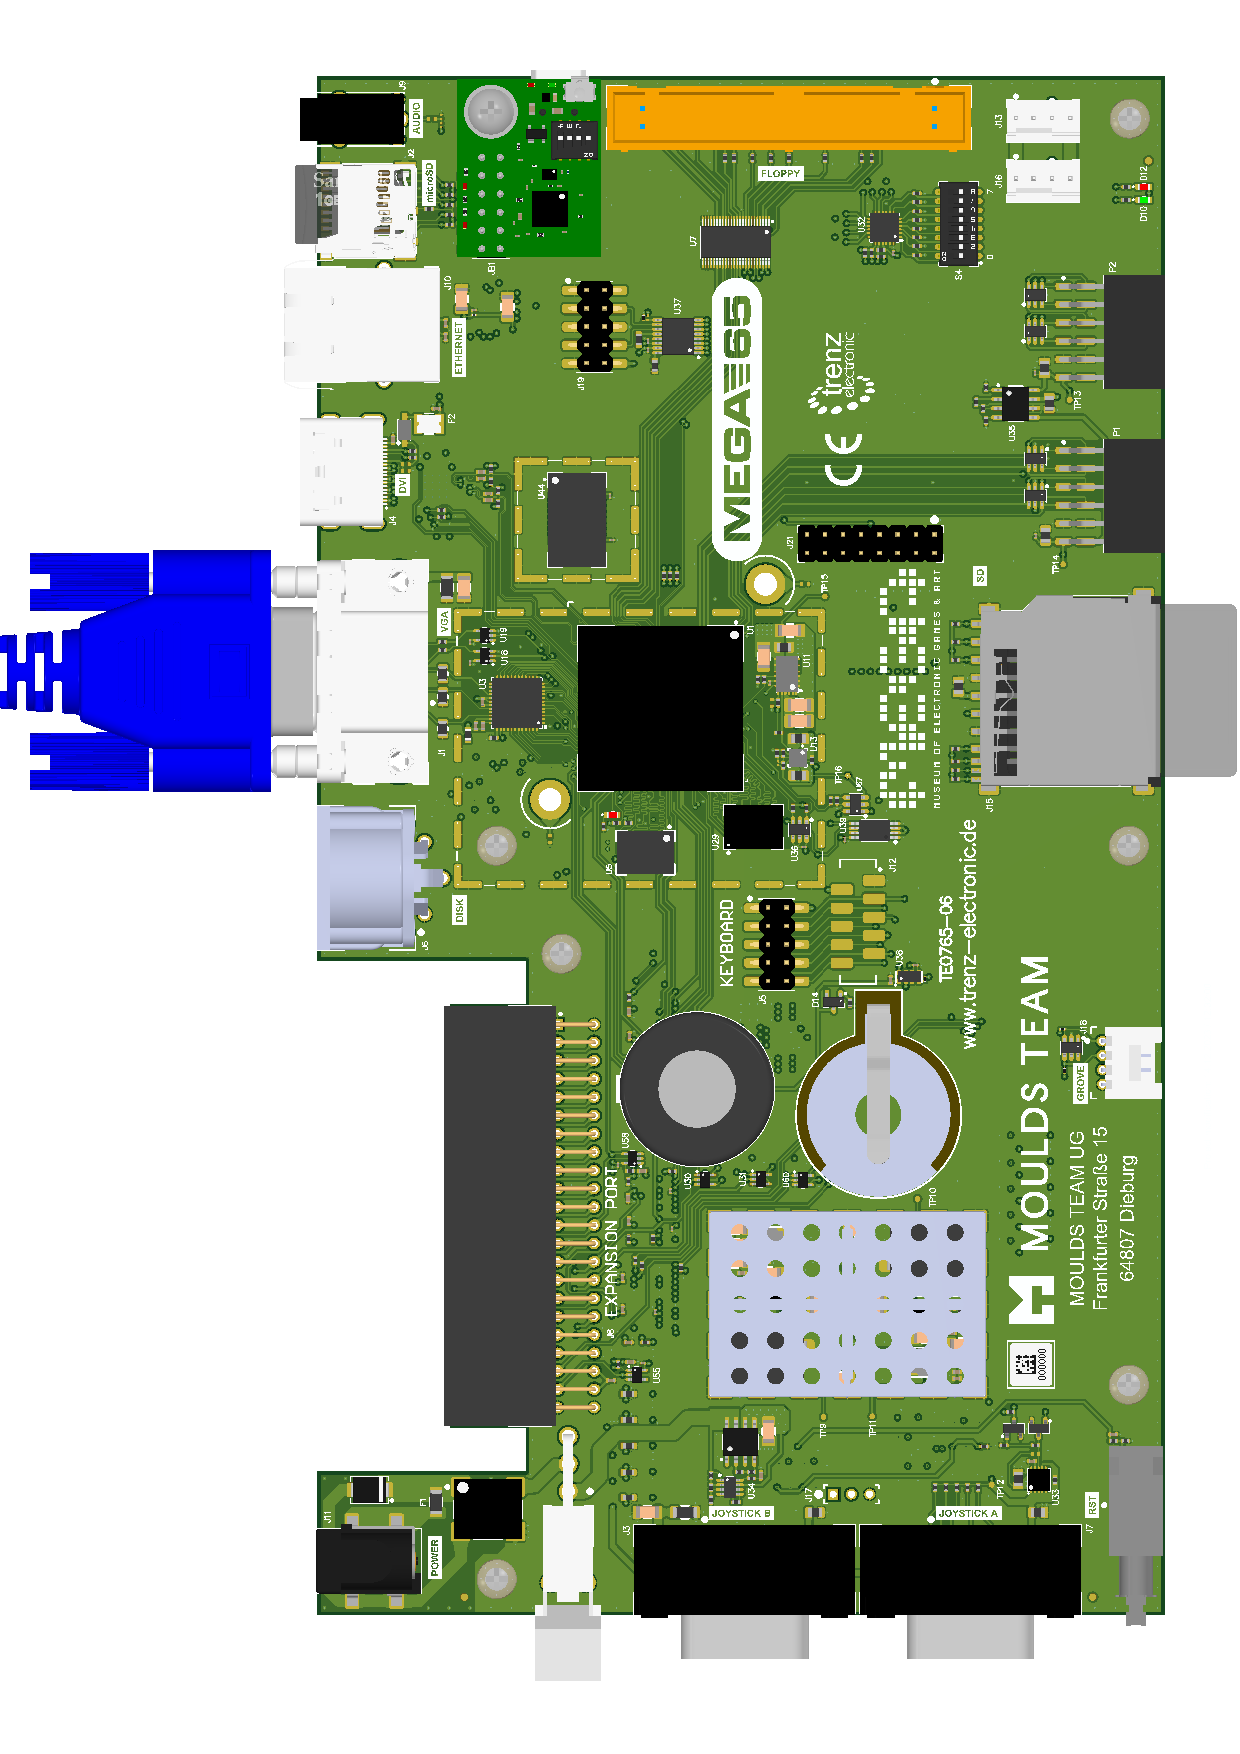
\includepdf[pages=-,turn=false]{assets/TE0765-06-front.PDF}
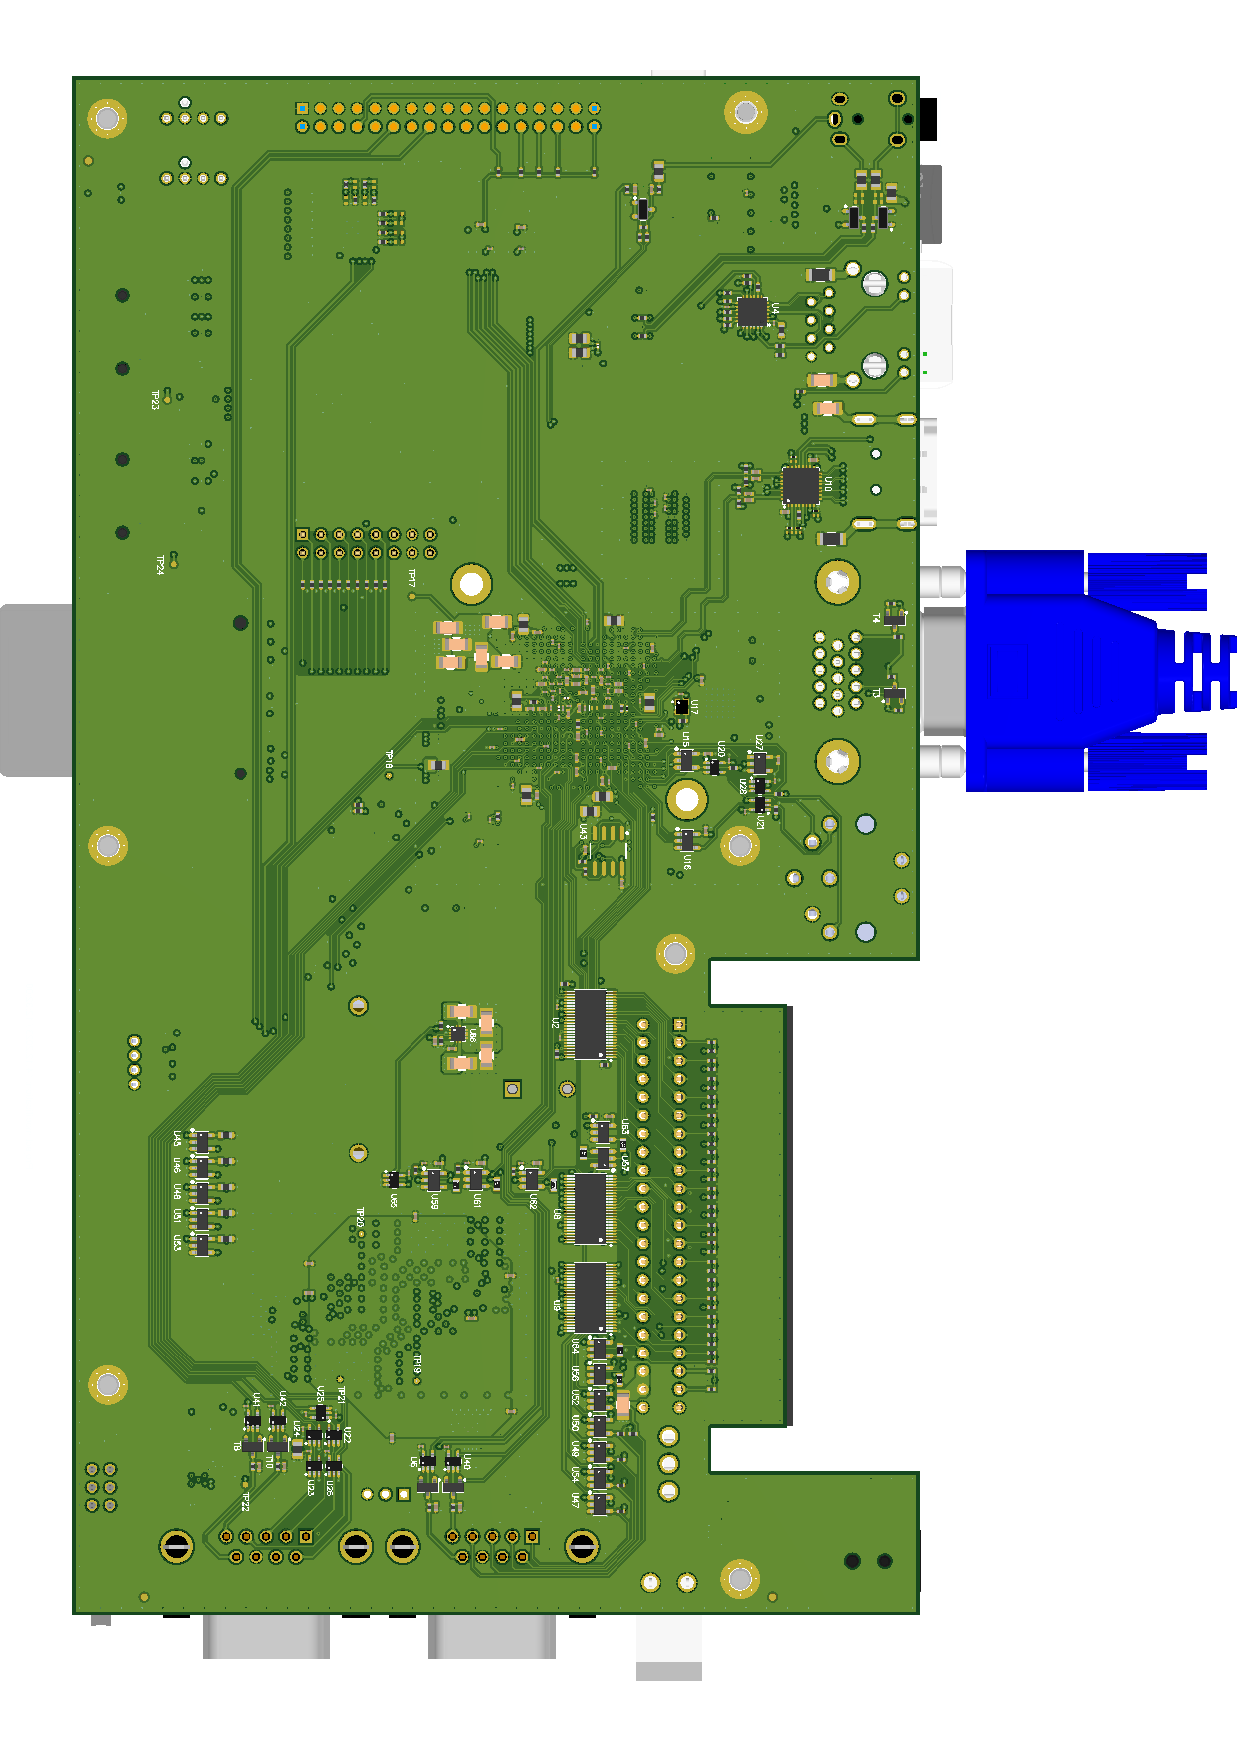
\includepdf[pages=-,turn=false]{assets/TE0765-06-back.PDF}
\section{MEGA65 R3 elektronisch schema}
\includepdf[landscape,pages=-,turn=false]{assets/TE0765-03.PDF}
\section{MEGA65 R2 elektronisch schema}
\includepdf[landscape,pages=-,turn=false]{assets/TE0765-02.PDF}
\section{Nexys Widget Board elektronisch schema}
\label{sec:nexyswidgetschematics}
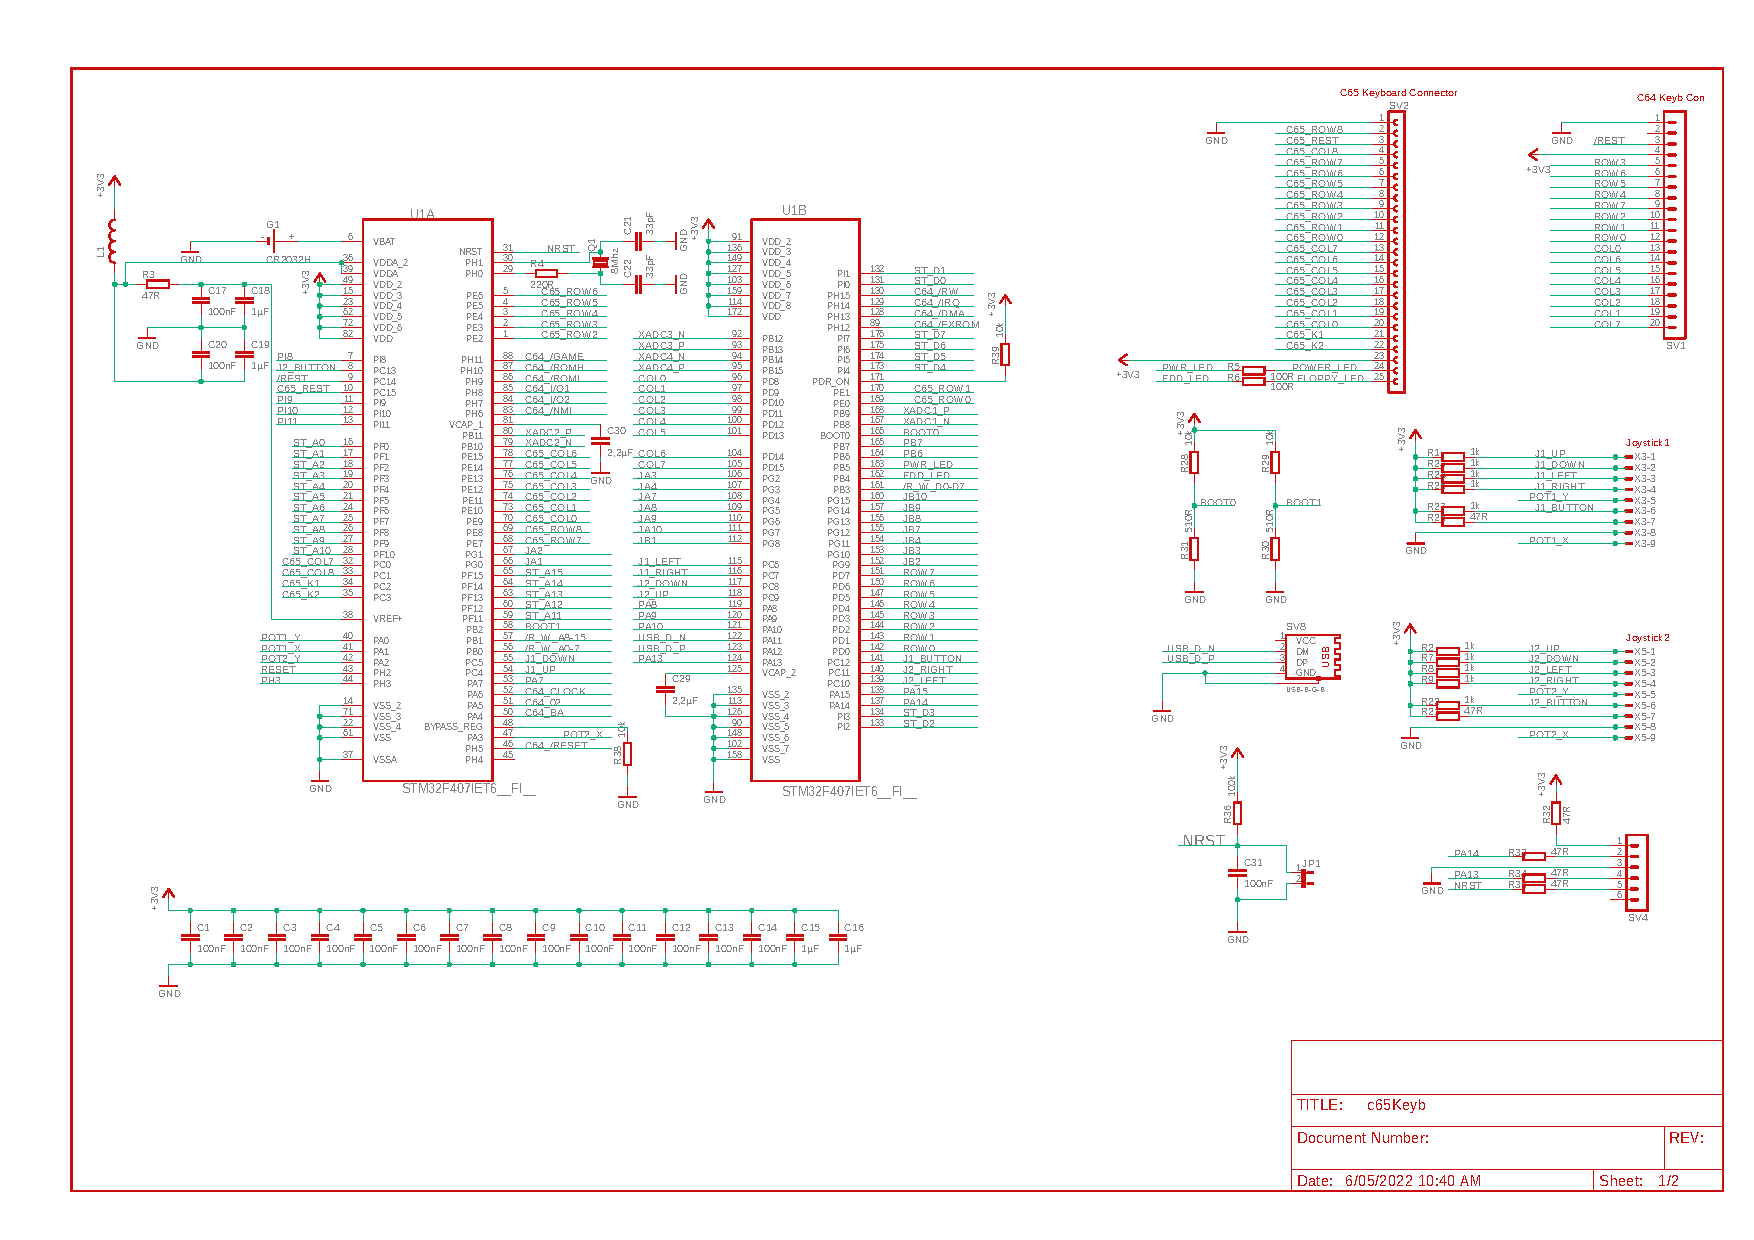
\includepdf[landscape,pages=-,turn=false]{assets/nexys-widget-board-sch.pdf}
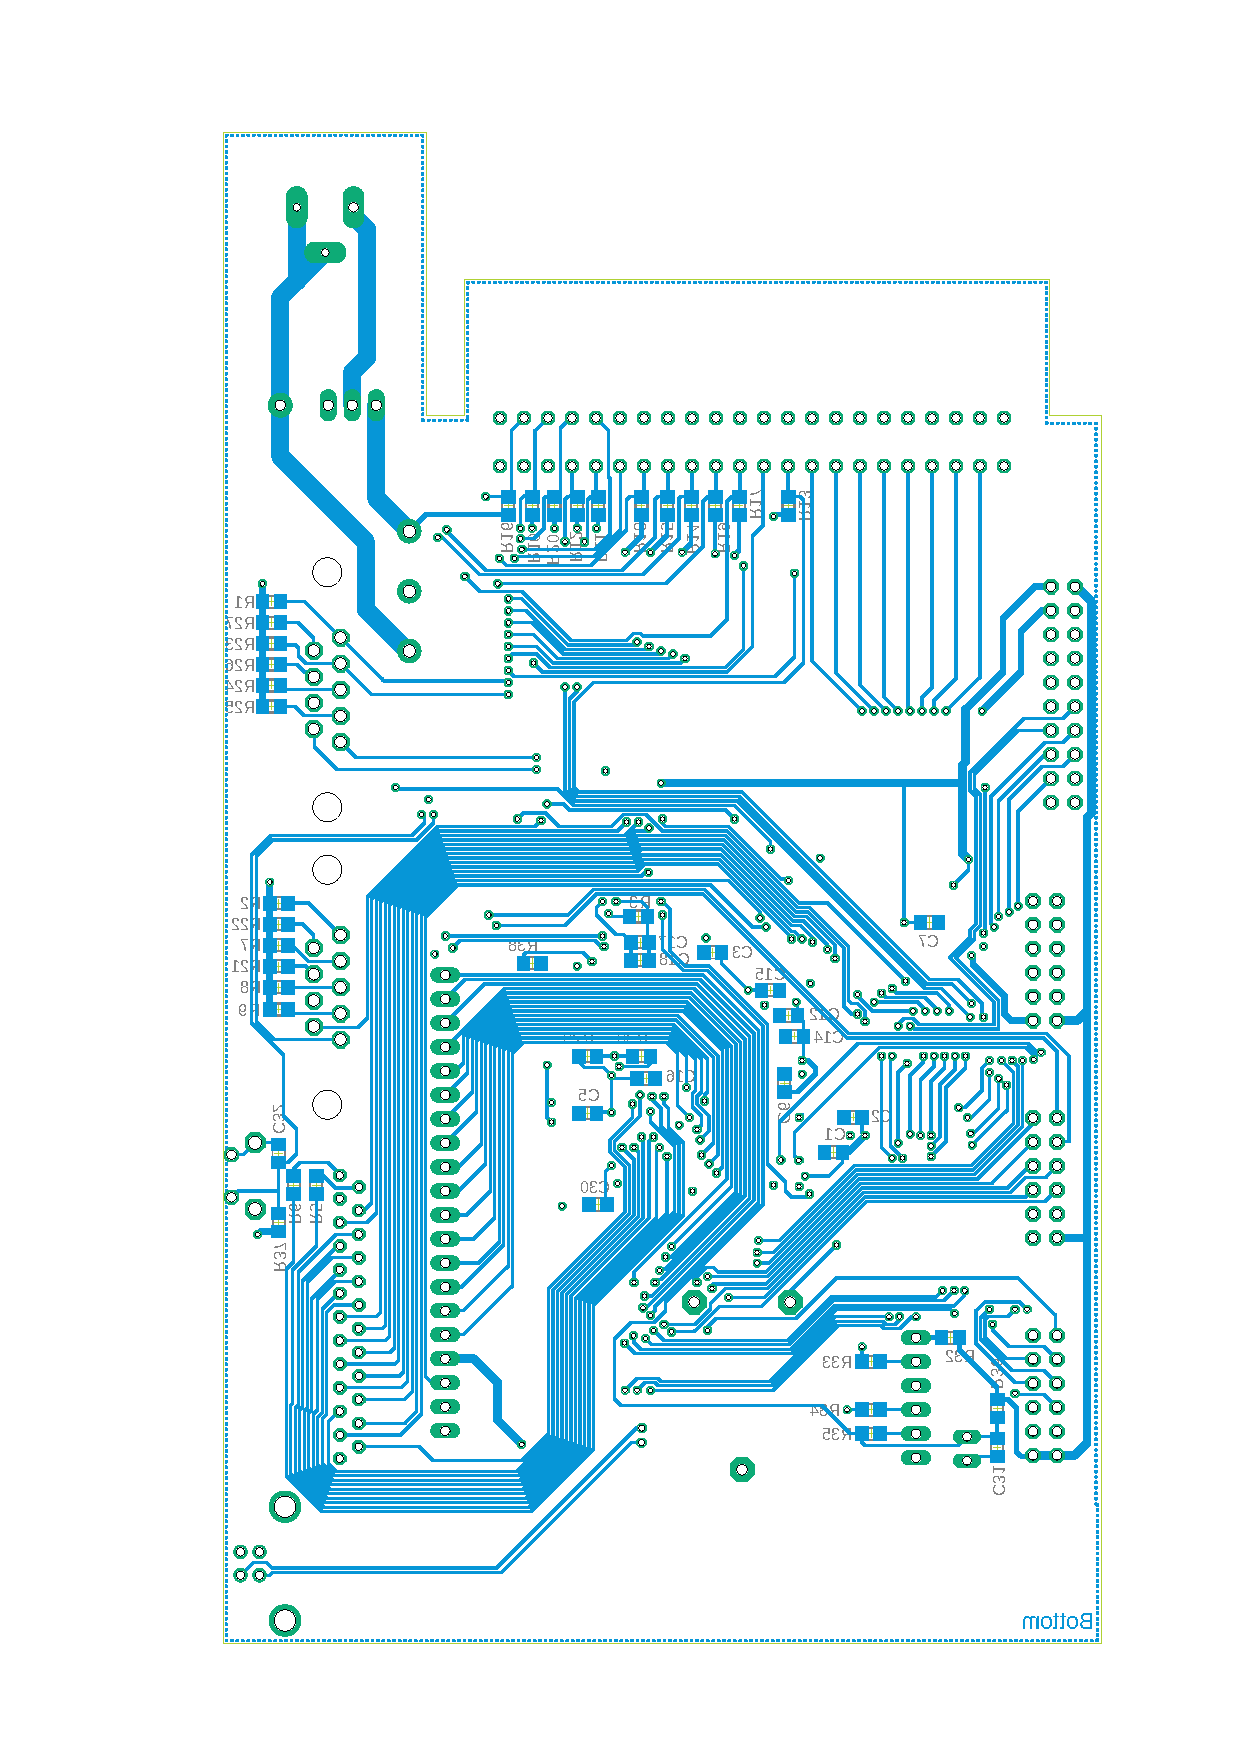
\includepdf[pages=-,turn=false]{assets/nexys-widget-board-pcb.pdf}

  \chapter{Steuners \& donateurs}


De MEGA65 zou niet tot stand zijn gekomen zonder de gulle steun van veel organisaties en individuen.

Wij stellen deze lijsten nog steeds samen; onze excuses indien u er nog niet in voorkomt. Indien u iemand kent die wij over het hoofd hebben gezien, laat het ons dan weten. Zo kunnen wij de bijdrage erkennen van iedereen die de MEGA65 mogelijk heeft gemaakt en die er het geweldige retrocomputingproject van heeft gemaakt dat de computer inmiddels is.

\section{Organisaties}

{\bf Het MEGA Museum of Electronic Games \& Art e.V. Duitsland} \\
\megakey{Alles}

{\bf Trenz Electronic, Duitsland} \\
\megakey{Moederbord}
\megakey{Fabricage}
\megakey{Verkoop}

{\bf Hintsteiner, Oostenrijk} \\
\megakey{Behuizing}

{\bf GMK, Duitsland} \\
\megakey{Toetsenbord}

{\bf KEVAG Telekom, Duitsland} \\
\megakey{Webhosting}

\newpage
\section{Bijdragers}

\begin{mega65thanks}

\begin{minipage}{\linewidth}
  {\large\bf Andreas Liebeskind} \\
  \textit{(libi in paradize)} \\
  Financieel directeur MEGA eV
\end{minipage}

\begin{minipage}{\linewidth}
  {\large\bf Thomas Hertzler} \\
  \textit{(grumpyninja)} \\
  Woordvoerder voor de VS
\end{minipage}

\begin{minipage}{\linewidth}
  {\large\bf Russell Peake} \\
  \textit{(rdpeake)} \\
  Bugherder
\end{minipage}

\begin{minipage}{\linewidth}
  {\large\bf Alexander Nik Petra} \\
  \textit{(n0d)} \\
  Vroeg ontwerp van de behuizing
\end{minipage}

\begin{minipage}{\linewidth}
  {\large\bf Ralph Egas} \\
  \textit{(0-limits)} \\
  Zakelijk adviseur
\end{minipage}

\begin{minipage}{\linewidth}
  {\large\bf Lucas Moss} \\  PCB-ontwerp voor de MEGAphone
\end{minipage}

\begin{minipage}{\linewidth}
  {\large\bf Daren Klamer} \\
  \textit{(Impakt)} \\
  Proeflezen van de handleiding
\end{minipage}

\begin{minipage}{\linewidth}
  {\large\bf Daniël Mantione}  \\
  \textit{(dmantione)} \\
  C64-hardwareguru
\end{minipage}

\columnbreak

\begin{minipage}{\linewidth}
  {\large\bf Dr. Canan Hastik} \\
  \textit{(indica)} \\
  Voorzitter MEGA eV
\end{minipage}

\begin{minipage}{\linewidth}
  {\large\bf Simon Jameson} \\
  \textit{(Shallan)} \\
  Platformverbeteringen
\end{minipage}

\begin{minipage}{\linewidth}
  {\large\bf Stephan Kleinert} \\
  \textit{(ubik)} \\
  Vernietiger van BASIC 10
\end{minipage}

\begin{minipage}{\linewidth}
  {\large\bf Wayne Johnson} \\
  \textit{(sausage)} \\
  Aanvullingen op de handleiding
\end{minipage}

\begin{minipage}{\linewidth}
  {\large\bf Raven L. A. Kleiss} \\
  \textit{(LAK132)} \\
  MegaWAT-presentatiesoftware
\end{minipage}

\begin{minipage}{\linewidth}
  {\large\bf Maurice van Gils }  \\
  \textit{(Maurice)}  \\
  BASIC 65-voorbeeldprogramma's
\end{minipage}

\begin{minipage}{\linewidth}
  {\large\bf Andrew Owen}  \\
  \textit{(Cheveron)} \\
  Toetsenbord, Sinclair-ondersteuning
\end{minipage}

\begin{minipage}{\linewidth}
  {\large\bf Adam Barnes}  \\
  \textit{(amb5l)} \\
  HDMI-expert en printplaatherziening
\end{minipage}

\begin{minipage}{\linewidth}
  {\large\bf Wayne Rittimann, Jr.} \\
  \textit{(johnwayner)} \\
  Bugverplettering op alle niveaus
\end{minipage}

\end{mega65thanks}


\newpage
\section{Steuners}

\begin{small}
% page 1
\setlength{\tabcolsep}{1mm}
\begin{tabular}{p{4cm}p{4cm}p{4cm}}
3c74ce64 & Arne Neumann & Christian Gräfe \\8-Bit Classics & Arne Richard Tyarks & Christian Heffner \\@11110110100 & Axel Klahr & Christian Kersting \\Aaron Smith & Balaz Ondrej & Christian Schiller \\Achim Mrotzek & Barry Thompson & Christian Streck \\Adolf Nefischer & Bartol Filipovic & Christian Weyer \\Adrian Esdaile & Benjamin Maas & Christian Wyk \\Adrien Guichard & Bernard Alaiz & Christoph Haug \\Ahmed Kablaoui & Bernhard Zorn & Christoph Huck \\Alan Bastian Witkowski & Bieno Marti-Braitmaier & Christoph Pross \\Alan Field & Bigby & Christopher Christopher \\Alastair Paulin-Campbell & Bill LaGrue & Christopher Kalk \\Alberto Mercuri & Bjoerg Stojalowski & Christopher Kohlert \\Alexander Haering & Björn Johannesson & Christopher Nelson \\Alexander Kaufmann & Bjørn Melbøe & Christopher Taylor \\Alexander Niedermeier & Bo Goeran Kvamme & Christopher Whillock \\Alexander Soppart & Boerge Noest & Claudio Piccinini \\Alfonso Ardire & Bolko Beutner & Claus Skrepek \\Amiga On The Lake & Brett Hallen & Collen Blijenberg \\André Kudra & Brian Gajewski & Constantine Lignos \\André Simeit & Brian Green & Crnjaninja \\André Wösten & Brian Juul Nielsen & Daniel Auger \\Andrea Farolfi & Brian Reiter & Daniel Julien \\Andrea Minutello & Bryan Pope & Daniel Lobitz \\Andreas Behr & Burkhard Franke & Daniel O'Connor \\Andreas Freier & Byron Goodman & Daniel Teicher \\Andreas Grabski & Cameron Roberton (KONG) & Daniel Tootill \\Andreas Millinger & Carl Angervall & Daniel Wedin \\Andreas Nopper & Carl Danowski & Daniele Benetti \\Andreas Ochs & Carl Stock & Daniele Gaetano Capursi \\Andreas Wendel Manufaktur & Carl Wall & Dariusz Szczesniak \\Andreas Zschunke & Carlo Pastore & Darrell Westbury \\Andrew Bingham & Carlos Silva & David Asenjo Raposo \\Andrew Dixon & Carsten Sørensen & David Dillard \\Andrew Mondt & Cenk Miroglu Miroglu & David Gorgon \\Andrzej Hłuchyj & Chang sik Park & David Norwood \\Andrzej Sawiniec & Charles A. Hutchins Jr. & David Raulo \\Andrzej Śliwa & Chris Guthrey & David Ross \\Anthony W. Leal & Chris Hooper & de voughn accooe \\Arkadiusz Bronowicki & Chris Stringer & Dean Scully \\Arkadiusz Kwasny & Christian Boettcher & Dennis Jeschke \\Arnaud Léandre & Christian Eick & Dennis Schaffers \\Arne Drews & Christian Gleinser & Dennis Schierholz \\
\end{tabular}
% page 2
\newpage
\setlength{\tabcolsep}{1mm}
\begin{tabular}{p{4cm}p{4cm}p{4cm}}
Dennis Schneck & Frank Haaland & Helge Förster \\denti & Frank Hempel & Hendrik Fensch \\Dick van Ginkel & Frank Koschel & Henning Harperath \\Diego Barzon & Frank Linhares & Henri Parfait \\Dierk Schneider & Frank Sleeuwaert & Henrik Kühn \\Dietmar Krueger & Frank Wolf & Holger Burmester \\Dietmar Schinnerl & FranticFreddie & Holger Sturk \\Dirk Becker & Fredrik Ramsberg & Howard Knibbs \\Dirk Wouters & Fridun Nazaradeh & Hubert de Hollain \\Domingo Fivoli & Friedel Kropp & Huberto Kusters \\DonChaos & Garrick West & Hugo Maria Gerardus v.d. Aa \\Donn Lasher & Gary Lake-Schaal & Humberto Castaneda \\Douglas Johnson & Gary Pearson & Ian Cross \\Dr. Leopold Winter & Gavin Jones & IDE64 Staff \\Dusan Sobotka & Geir Sigmund Straume & Igor Ianov \\Earl Woodman & Gerd Mitlaender & Igor Kurtes \\Ed Reilly & Giampietro Albiero & Immo Beutler \\Edoardo Auteri & Giancarlo Valente & Ingo Katte \\Eduardo Gallardo & Gianluca Girelli & Ingo Keck \\Eduardo Luis Arana & Giovanni Medina & Insanely Interested Publishing \\Eirik Juliussen Olsen & Glen Fraser & IT-Dienstleistungen Obsieger \\Emilio Monelli & Glen R Perye III & Ivan Elwood \\EP Technical Services & Glenn Main & Jaap HUIJSMAN \\Epic Sound & Gordon Rimac & Jace Courville \\Erasmus Kuhlmann & GRANT BYERS & Jack Wattenhofer \\ergoGnomik & Grant Louth & Jakob Schönpflug \\Eric Hilaire & Gregor Bubek & Jakub Tyszko \\Eric Hildebrandt & Gregor Gramlich & James Hart \\Eric Hill & Guido Ling & James Marshburn \\Eric Jutrzenka & Guido von Gösseln & James McClanahan \\Erwin Reichel & Guillaume Serge & James Sutcliffe \\Espen Skog & Gunnar Hemmerling & Jan Bitruff \\Evangelos Mpouras & Günter Hummel & Jan Hildebrandt \\Ewan Curtis & Guy Simmons & Jan Iemhoff \\Fabio Zanicotti & Guybrush Threepwood & Jan Kösters \\Fabrizio Di Dio & Hakan Blomqvist & Jan Peter Borsje \\Fabrizio Lodi & Hans Pronk & Jan Schulze \\FARA Gießen GmbH & Hans-Jörg Nett & Jan Stoltenberg-Lerche \\FeralChild & Hans-Martin Zedlitz & Janne Tompuri \\First Choice Auto's & Harald Dosch & Jannis Schulte \\Florian Rienhardt & Harri Salokorpi & Jari Loukasmäki \\Forum64. de & Harry Culpan & Jason Smith \\Francesco Baldassarri & Harry Venema & Javier Gonzalez Gonzalez \\Frank Fechner & Heath Gallimore & Jean-Paul Lauque \\Frank Glaush & Heinz Roesner & Jeffrey van der Schilden \\Frank Gulasch & Heinz Stampfli & Jens Schneider \\
\end{tabular}
% page 3
\newpage
\setlength{\tabcolsep}{1mm}
\begin{tabular}{p{4cm}p{4cm}p{4cm}}
Jens-Uwe Wessling & Kenneth Joensson & Marco Cappellari \\Jesse DiSimone & Kevin Edwards & Marco Rivela \\Jett Adams & Kevin Thomasson & Marco van de Water \\Johan Arneklev & Kim Jorgensen & Marcus Gerards \\Johan Berntsson & Kim Rene Jensen & Marcus Herbert \\Johan Svensson & Kimmo Hamalainen & Marcus Linkert \\Johannes Fitz & Konrad Buryło & Marek Pernicky \\John Cook & Kosmas Einbrodt & Mario Esposito \\John Deane & Kurt Klemm & Mario Fetka \\John Dupuis & Lachlan Glaskin & Mario Teschke \\John Nagi & Large bits collider & Mariusz Tymków \\John Rorland & Lars Becker & Mark Adams \\John Sargeant & Lars Edelmann & Mark Anderson \\John Traeholt & Lars Slivsgaard & Mark Green \\Jon Sandelin & Lasse Lambrecht & Mark Hucker \\Jonas Bernemann & Lau Olivier & Mark Leitiger \\Jonathan Prosise & Lee Chatt & Mark Spezzano \\Joost Honig & Loan Leray & Mark Watkin \\Jordi Pakey-Rodriguez & Lorenzo Quadri & Marko Rizvic \\Jöre Weber & Lorenzo Travagli & Markus Bieler \\Jörg Jungermann & Lorin Millsap & Markus Bonet \\Jörg Schaeffer & Lothar James Foss & Markus Dauberschmidt \\Jörg Weese & Lothar Serra Mari & Markus Fehr \\Josef Hesse & Luca Papinutti & Markus Fuchs \\Josef Soucek & Ludek Smetana & Markus Guenther-Hirn \\Josef Stohwasser & Lukas Burger & Markus Liukka \\Joseph Clifford & Lutz-Peter Buchholz & Markus Merz \\Joseph Gerth & Luuk Spaetgens & Markus Roesgen \\Jovan Crnjanin & Mad Web Skills & Markus Uttenweiler \\Juan Pablo Schisano & MaDCz & Martin Bauhuber \\Juan S. Cardona Iguina & Magnus Wiklander & Martin Benke \\JudgeBeeb & Maik Diekmann & Martin Gendera \\Juliussen Olsen & Malte Mundt & Martin Groß \\Juna Luis Fernandez Garcia & Manfred Wittemann & Martin Gutenbrunner \\Jürgen Endras & Manuel Beckmann & Martin Johansen \\Jürgen Herm Stapelberg & Manzano Mérida & Martin Marbach \\Jyrki Laurila & Marc "3D-vice" Schmitt & Martin Sonnleitner \\Kai Pernau & Marc Bartel & Martin Steffen \\Kalle Pöyhönen & Marc Jensen & Marvin Hardy \\Karl Lamford & Marc Schmidt & Massimo Villani \\Karl-Heinz Blum & Marc Theunissen & Mathias Dellacherie \\Karsten Engstler & Marc Tutor & Mathieu Chouinard \\Karsten Westebbe & Marc Wink & Matthew Adams \\katarakt & Marcel Buchtmann & Matthew Browne \\Keith McComb & Marcel Kante & Matthew Carnevale \\Kenneth Dyke & Marco Beckers & Matthew Palmer \\
\end{tabular}
% page 4
\newpage
\setlength{\tabcolsep}{1mm}
\begin{tabular}{p{4cm}p{4cm}p{4cm}}
Matthew Santos & Michele Porcu & Paul Jackson \\Matthias Barthel & Miguel Angel Rodriguez Jodar & Paul Johnson \\Matthias Dolenc & Mikael Lund & Paul Kuhnast (mindrail) \\Matthias Fischer & Mike Betz & Paul Massay \\Matthias Frey & Mike Kastrantas & Paul Westlake \\Matthias Grandis & Mike Pikowski & Paul Woegerer \\Matthias Guth & Mikko Hämäläinen & Pauline Brasch \\Matthias Lampe & Mikko Suontausta & Paulo Apolonia \\Matthias Meier & Mirko Roller & Pete Collin \\Matthias Mueller & Miroslav Karkus & Pete of Retrohax.net \\Matthias Nofer & Morgan Antonsson & Peter Eliades \\Matthias Schonder & Moritz & Peter Gries \\Maurice Al-Khaliedy & Morten Nielsen & Peter Habura \\Max Ihlenfeldt & MUBIQUO APPS,SL & Peter Herklotz \\Meeso Kim & Myles Cameron-Smith & Peter Huyoff \\Michael Dailly & Neil Moore & Peter Knörzer \\Michael Dötsch & Nelson & Peter Leswell \\Michael Dreßel & neoman & Peter Weile \\Michael Fichtner & Nicholas Melnick & Petri Alvinen \\Michael Fong & Nikolaj Brinch Jørgensen & Philip Marien \\Michael Geoffrey Stone & Nils Andreas & Philip Timmermann \\Michael Gertner & Nils Eilers & Philipp Rudin \\Michael Grün & Nils Hammerich & Pierre Kressmann \\Michael Habel & Nils77 & Pieter Labie \\Michael Härtig & Norah Smith & Piotr Kmiecik \\Michael Haynes & Norman King & Power-on.at \\Michael J Burkett & Normen Zoch & Przemysław Safonow \\Michael Jensen & Olaf Grunert & Que Labs \\Michael Jurisch & Ole Eitels & R Welbourn \\Michael Kappelgaard & Oliver Boerner & R-Flux \\Michael Kleinschmidt & Oliver Brüggmann & Rafał Michno \\Michael Lorenz & Oliver Graf & Rainer Kappler \\Michael Mayerhofer & Oliver Smith & Rainer Kopp \\Michael Nurney & Olivier Bori & Rainer Weninger \\Michael Rasmussen & ONEPSI LLC & Ralf Griewel \\Michael Richmond & oRdYNe & Ralf Pöscha \\Michael Sachse & Osaühing Trioflex & Ralf Reinhardt \\Michael Sarbak & OSHA-PROS USA & Ralf Schenden \\Michael Schneider & Padawer & Ralf Smolarek \\Michael Scholz & Patrick Becher & Ralf Zenker \\Michael Timm & Patrick Bürckstümmer & Ralph Bauer \\Michael Traynor & Patrick de Zoete & Ralph Wernecke \\Michael Whipp & Patrick Toal & Rédl Károly \\Michal Ursiny & Patrick Vogt & Reiner Lanowski \\Michele Chiti & Paul Alexander Warren & Remi Veilleux \\Michele Perini & Paul Gerhardt (KONG) & Riccardo Bianchi \\
\end{tabular}
% page 5
\newpage
\setlength{\tabcolsep}{1mm}
\begin{tabular}{p{4cm}p{4cm}p{4cm}}
Richard Englert & Sigurbjorn Larusson & Thomas Niemann \\Richard Good & Sigurdur Finnsson & Thomas Scheelen \\Richard Menedetter & Simon Lawrence & Thomas Schilling \\Richard Sopuch & Simon Wolf & Thomas Tahsin-Bey \\Rick Reynolds & spreen.digital & Thomas Walter \\Rico Gruninger & Stefan Haberl & Thomas Wirtzmann \\Rob Dean & Stefan Kramperth & Thorsten Knoll \\Robert Bernardo & Stefan Richter & Thorsten Nolte \\Robert Eaglestone & Stefan Schultze & Tim Krome \\Robert Grasböck & Stefan Sonnek & Tim Waite \\Robert Miles & Stefan Theil & Timo Weirich \\Robert Schwan & Stefan Vrampe & Timothy Blanks \\Robert Shively & Stefano Canali & Timothy Henson \\Robert Tangmar & Stefano Mozzi & Timothy Prater \\Robert Trangmar & Steffen Reiersen & Tobias Butter \\Rodney Xerri & Stephan Bielmann & Tobias Heim \\Roger Olsen & Stephen Jones & Tobias Köck \\Roger Pugh & Stephen Kew & Tobias Lüthi \\Roland Attila Kett & Steve Gray & Tommi Vasarainen \\Roland Evers & Steve Kurlin & Toni Ammer \\Roland Schatz & Steve Lemieux & Tore Olsen \\Rolf Hass & Steven Combs & Torleif Strand \\Ronald Cooper & Stewart Dunn & Torsten Schröder \\Ronald Hunn & Stuart Marsh & Tuan Nguyen \\Ronny Hamida & Sven Neumann & Uffe Jakobsen \\Ronny Preiß & Sven Stache & Ulrich Hintermeier \\Roy van Zundert & Sven Sternberger & Ulrich Nieland \\Rüdiger Wohlfromm & Sven Wiegand & Ulrik Kruse \\Ruediger Schlenter & Szabolcs Bence & Urban Lindeskog \\Rutger WIllemsen & Tantrumedia Limited & Ursula Förstle \\Sampo Peltonen & Techvana Operations Ltd. & Uwe Anfang \\Sarmad Gilani & Teddy Turmeaux & Uwe Boschanski \\SAS74 & Teemu Korvenpää & Vedran Vrbanc \\Sascha Hesse & The Games Foundation & Verm Project \\Scott Halman & Thierry Supplisson & Wayne Rittimann \\Scott Hollier & Thieu-Duy Thai & Wayne Sander \\Scott Robison & Thomas Bierschenk & Wayne Steele \\Sebastian Baranski & Thomas Edmister & Who Knows \\Sebastian Bölling & Thomas Frauenknecht & Winfried Falkenhahn \\Sebastian Felzmann & Thomas Gitzen & Wolfgang Becker \\Sebastian Lipp & Thomas Gruber & Wolfgang Stabla \\Sebastian Rakel & Thomas Haidler & Worblehat \\Şemseddin Moldibi & Thomas Jager & www.patop69.net \\Seth Morabito & Thomas Karlsen & Yan B \\Shawn McKee & Thomas Laskowski & Zoltan Markus \\Siegfried Hartmann & Thomas Marschall & Zsolt Zsila \\Zytex Online Store &  &  \\
\end{tabular}
\end{small}
\ifdefined\printmanual
\else
\setstretch{1}
\fi



\nocite{*}
\bibliographystyle{IEEEtran-nl}
\bibliography{references}

\pagenumbering[Index]{bychapter}
\printindex

\cleardoublepage

% Temporarily enlarge this page to push
%% down the bottom margin
\enlargethispage{3\baselineskip}
\thispagestyle{empty}
\pagecolor[HTML]{2244FF}

\begin{center}
\begin{minipage}{.8\textwidth}
\color{white}
\begin{center}
{ \huge\bfseries\sffamily\color{white}Over het grote Mega65-boek }
\end{center}

\vspace{3mm}
\hrulefill
\vspace{3mm}

{
C64- en C65-programma- en randapparatuurcompatibiliteit, prachtig geluid, echte arcadeklasse-grafiek, een
prachtig afgewerkt stuk hardware met volledig mechanisch toetsenbord en uitgebreide netwerkmogelijkheden,
en een van de snelste verkrijgbare 6502-klasseprocessors maken de MEGA65 werkelijk uniek voor thuis-, bedrijfs-
of educatief gebruik.

\vspace{2mm}

{\bf Alles over de Mega65} verzamelt in één groot boekdeel alle informatie die u over uw MEGA65
moet weten.  Door alle essentiële informatie uit de diverse MEGA65-gebruikershandleidingen en
-naslagwerken op één plek te bundelen, biedt dit boek gedetailleerde informatie over elk onderwerp, waaronder
BASIC-programmering, geluid, grafiek, netwerken, assembleertaalprogrammering, platformonafhankelijke ontwik-
keling, waaronder het gebruik van hogere programmeertalen zoals C of KickC, de krachtige 8-bitschipset van de
MEGA65 en hoe u de krachtige FPGA-core kunt gebruiken om andere computersystemen te implementeren.

\vspace{2mm}

Dit boek is het onmisbare naslagwerk voor de MEGA65, dat elke gebruiker, of hij nu beginner of gevorderd is,
bij zich zou moeten hebben wanneer hij het volledige potentieel van de MEGA65 verkent.

\vspace{2mm}

Met auteurs waaronder professionele schrijvers, universiteitsdocenten en 8-bitexperts is de inhoud zowel
toegankelijk als uitgebreid.  Beginners vinden gedetailleerde uitleg over hoe ze kunnen beginnen, terwijl
gevorderde gebruikers zeer gedetailleerde technische informatie vinden over de innerlijke werking van  elk
aspect van de MEGA65.

\vspace{2mm}

Kortom, dit boek is ontworpen om u het maximale uit de uitgebreide mogelijkheden van de MEGA65 te laten halen.
}

\end{minipage}
\end{center}

\vspace*{\stretch{1}}

\begin{center}
\colorbox{white}{\EANisbn[SC4,ISBN=123-45-67890-12-8]}

\vspace*{\baselineskip}

\textbf{\textcolor{white}{het MEGA Museum of Electronic Games \& Art e.V. \url{http://mega65.org}}}

\textbf{\textcolor{white}{Redactie: Univ. hoofddoc. Dr. Paul Gardner-Stephen.}}

\textbf{\textcolor{white}{Vertaling: Daniël Mantione.}}
\end{center}



\end{document}


